\documentclass[twoside]{book}

% Packages required by doxygen
\usepackage{fixltx2e}
\usepackage{calc}
\usepackage{doxygen}
\usepackage[export]{adjustbox} % also loads graphicx
\usepackage{graphicx}
\usepackage[utf8]{inputenc}
\usepackage{makeidx}
\usepackage{multicol}
\usepackage{multirow}
\PassOptionsToPackage{warn}{textcomp}
\usepackage{textcomp}
\usepackage[nointegrals]{wasysym}
\usepackage[table]{xcolor}

% Font selection
\usepackage[T1]{fontenc}
\usepackage[scaled=.90]{helvet}
\usepackage{courier}
\usepackage{amssymb}
\usepackage{sectsty}
\renewcommand{\familydefault}{\sfdefault}
\allsectionsfont{%
  \fontseries{bc}\selectfont%
  \color{darkgray}%
}
\renewcommand{\DoxyLabelFont}{%
  \fontseries{bc}\selectfont%
  \color{darkgray}%
}
\newcommand{\+}{\discretionary{\mbox{\scriptsize$\hookleftarrow$}}{}{}}

% Page & text layout
\usepackage{geometry}
\geometry{%
  a4paper,%
  top=2.5cm,%
  bottom=2.5cm,%
  left=2.5cm,%
  right=2.5cm%
}
\tolerance=750
\hfuzz=15pt
\hbadness=750
\setlength{\emergencystretch}{15pt}
\setlength{\parindent}{0cm}
\setlength{\parskip}{3ex plus 2ex minus 2ex}
\makeatletter
\renewcommand{\paragraph}{%
  \@startsection{paragraph}{4}{0ex}{-1.0ex}{1.0ex}{%
    \normalfont\normalsize\bfseries\SS@parafont%
  }%
}
\renewcommand{\subparagraph}{%
  \@startsection{subparagraph}{5}{0ex}{-1.0ex}{1.0ex}{%
    \normalfont\normalsize\bfseries\SS@subparafont%
  }%
}
\makeatother

% Headers & footers
\usepackage{fancyhdr}
\pagestyle{fancyplain}
\fancyhead[LE]{\fancyplain{}{\bfseries\thepage}}
\fancyhead[CE]{\fancyplain{}{}}
\fancyhead[RE]{\fancyplain{}{\bfseries\leftmark}}
\fancyhead[LO]{\fancyplain{}{\bfseries\rightmark}}
\fancyhead[CO]{\fancyplain{}{}}
\fancyhead[RO]{\fancyplain{}{\bfseries\thepage}}
\fancyfoot[LE]{\fancyplain{}{}}
\fancyfoot[CE]{\fancyplain{}{}}
\fancyfoot[RE]{\fancyplain{}{\bfseries\scriptsize Generated by Doxygen }}
\fancyfoot[LO]{\fancyplain{}{\bfseries\scriptsize Generated by Doxygen }}
\fancyfoot[CO]{\fancyplain{}{}}
\fancyfoot[RO]{\fancyplain{}{}}
\renewcommand{\footrulewidth}{0.4pt}
\renewcommand{\chaptermark}[1]{%
  \markboth{#1}{}%
}
\renewcommand{\sectionmark}[1]{%
  \markright{\thesection\ #1}%
}

% Indices & bibliography
\usepackage{natbib}
\usepackage[titles]{tocloft}
\setcounter{tocdepth}{3}
\setcounter{secnumdepth}{5}
\makeindex

% Hyperlinks (required, but should be loaded last)
\usepackage{ifpdf}
\ifpdf
  \usepackage[pdftex,pagebackref=true]{hyperref}
\else
  \usepackage[ps2pdf,pagebackref=true]{hyperref}
\fi
\hypersetup{%
  colorlinks=true,%
  linkcolor=blue,%
  citecolor=blue,%
  unicode%
}

% Custom commands
\newcommand{\clearemptydoublepage}{%
  \newpage{\pagestyle{empty}\cleardoublepage}%
}

\usepackage{caption}
\captionsetup{labelsep=space,justification=centering,font={bf},singlelinecheck=off,skip=4pt,position=top}

%===== C O N T E N T S =====

\begin{document}

% Titlepage & ToC
\hypersetup{pageanchor=false,
             bookmarksnumbered=true,
             pdfencoding=unicode
            }
\pagenumbering{alph}
\begin{titlepage}
\vspace*{7cm}
\begin{center}%
{\Large Brain\+Harmonics \\[1ex]\large 0.\+1 }\\
\vspace*{1cm}
{\large Generated by Doxygen 1.8.13}\\
\end{center}
\end{titlepage}
\clearemptydoublepage
\pagenumbering{roman}
\tableofcontents
\clearemptydoublepage
\pagenumbering{arabic}
\hypersetup{pageanchor=true}

%--- Begin generated contents ---
\chapter{Namespace Index}
\section{Namespace List}
Here is a list of all namespaces with brief descriptions\+:\begin{DoxyCompactList}
\item\contentsline{section}{\mbox{\hyperlink{namespacebhcompute}{bhcompute}} }{\pageref{namespacebhcompute}}{}
\item\contentsline{section}{\mbox{\hyperlink{namespacestd}{std}} }{\pageref{namespacestd}}{}
\end{DoxyCompactList}

\chapter{Hierarchical Index}
\section{Class Hierarchy}
This inheritance list is sorted roughly, but not completely, alphabetically\+:\begin{DoxyCompactList}
\item Ar\+Action\begin{DoxyCompactList}
\item \contentsline{section}{mapper}{\pageref{classmapper}}{}
\end{DoxyCompactList}
\item \contentsline{section}{Dimension\+:\+:Counter\+Adjustment}{\pageref{structDimension_1_1CounterAdjustment}}{}
\item \contentsline{section}{Graph$<$ L $>$}{\pageref{structGraph}}{}
\item \contentsline{section}{std\+:\+:hash$<$ tuple$<$ int, int $>$ $>$}{\pageref{structstd_1_1hash_3_01tuple_3_01int_00_01int_01_4_01_4}}{}
\item \contentsline{section}{Messages}{\pageref{classMessages}}{}
\item \contentsline{section}{Synapse\+:\+:Nearby\+Neuron}{\pageref{structSynapse_1_1NearbyNeuron}}{}
\item \contentsline{section}{Interneuron\+Space\+:\+:Nearby\+Neuron}{\pageref{structInterneuronSpace_1_1NearbyNeuron}}{}
\item \contentsline{section}{node}{\pageref{classnode}}{}
\item \contentsline{section}{Neuron\+:\+:Object\+Connection}{\pageref{structNeuron_1_1ObjectConnection}}{}
\item \contentsline{section}{Soma\+:\+:Object\+Connection}{\pageref{structSoma_1_1ObjectConnection}}{}
\item \contentsline{section}{Cognitive\+Network\+:\+:Orbital\+Connection}{\pageref{structCognitiveNetwork_1_1OrbitalConnection}}{}
\item \contentsline{section}{Priority\+Queue$<$ T, Number $>$}{\pageref{structPriorityQueue}}{}
\item \contentsline{section}{Synapse\+:\+:s\+\_\+\+Bind\+List}{\pageref{structSynapse_1_1s__BindList}}{}
\item \contentsline{section}{Interneuron\+Space\+:\+:s\+\_\+\+Bind\+List}{\pageref{structInterneuronSpace_1_1s__BindList}}{}
\item \contentsline{section}{Sniffex\+:\+:sniff\+\_\+ethernet}{\pageref{structSniffex_1_1sniff__ethernet}}{}
\item \contentsline{section}{Sniffex\+:\+:sniff\+\_\+ip}{\pageref{structSniffex_1_1sniff__ip}}{}
\item \contentsline{section}{Sniffex\+:\+:sniff\+\_\+tcp}{\pageref{structSniffex_1_1sniff__tcp}}{}
\item \contentsline{section}{Sniffex}{\pageref{classSniffex}}{}
\item \contentsline{section}{Square\+Grid}{\pageref{structSquareGrid}}{}
\begin{DoxyCompactList}
\item \contentsline{section}{Grid\+With\+Weights}{\pageref{structGridWithWeights}}{}
\item \contentsline{section}{Grid\+With\+Weights}{\pageref{structGridWithWeights}}{}
\end{DoxyCompactList}
\item \contentsline{section}{Universe}{\pageref{classUniverse}}{}
\begin{DoxyCompactList}
\item \contentsline{section}{Abstraction}{\pageref{classAbstraction}}{}
\item \contentsline{section}{App\+Timer}{\pageref{classAppTimer}}{}
\item \contentsline{section}{Cognitive\+Network}{\pageref{classCognitiveNetwork}}{}
\begin{DoxyCompactList}
\item \contentsline{section}{Cognitive\+Input}{\pageref{classCognitiveInput}}{}
\item \contentsline{section}{Cognitive\+Output}{\pageref{classCognitiveOutput}}{}
\item \contentsline{section}{Interneuron\+Space}{\pageref{classInterneuronSpace}}{}
\begin{DoxyCompactList}
\item \contentsline{section}{Schwann\+Cell}{\pageref{classSchwannCell}}{}
\end{DoxyCompactList}
\item \contentsline{section}{Myelin\+Sheath}{\pageref{classMyelinSheath}}{}
\item \contentsline{section}{Neuron}{\pageref{classNeuron}}{}
\begin{DoxyCompactList}
\item \contentsline{section}{Membrane}{\pageref{classMembrane}}{}
\begin{DoxyCompactList}
\item \contentsline{section}{Membrane\+Channel}{\pageref{classMembraneChannel}}{}
\end{DoxyCompactList}
\item \contentsline{section}{Soma}{\pageref{classSoma}}{}
\begin{DoxyCompactList}
\item \contentsline{section}{Axon\+Hillock}{\pageref{classAxonHillock}}{}
\begin{DoxyCompactList}
\item \contentsline{section}{Axon}{\pageref{classAxon}}{}
\item \contentsline{section}{Axon\+Branch}{\pageref{classAxonBranch}}{}
\item \contentsline{section}{Axon\+Bouton}{\pageref{classAxonBouton}}{}
\item \contentsline{section}{Synaptic\+Vesicle}{\pageref{classSynapticVesicle}}{}
\end{DoxyCompactList}
\item \contentsline{section}{Dendrite}{\pageref{classDendrite}}{}
\begin{DoxyCompactList}
\item \contentsline{section}{Dendrite\+Branch}{\pageref{classDendriteBranch}}{}
\item \contentsline{section}{Dendrite\+Cleft}{\pageref{classDendriteCleft}}{}
\item \contentsline{section}{Neuroreceptor}{\pageref{classNeuroreceptor}}{}
\end{DoxyCompactList}
\end{DoxyCompactList}
\end{DoxyCompactList}
\item \contentsline{section}{Neurotransmitter}{\pageref{classNeurotransmitter}}{}
\item \contentsline{section}{Orbital}{\pageref{classOrbital}}{}
\item \contentsline{section}{Spike}{\pageref{classSpike}}{}
\item \contentsline{section}{Synapse}{\pageref{classSynapse}}{}
\end{DoxyCompactList}
\item \contentsline{section}{Composite\+Force\+Particle}{\pageref{classCompositeForceParticle}}{}
\item \contentsline{section}{Dimension}{\pageref{classDimension}}{}
\item \contentsline{section}{Elementary\+Force}{\pageref{classElementaryForce}}{}
\item \contentsline{section}{Elementary\+Particle}{\pageref{classElementaryParticle}}{}
\item \contentsline{section}{Law}{\pageref{classLaw}}{}
\item \contentsline{section}{Line}{\pageref{classLine}}{}
\item \contentsline{section}{Matter}{\pageref{classMatter}}{}
\item \contentsline{section}{Monomer}{\pageref{classMonomer}}{}
\begin{DoxyCompactList}
\item \contentsline{section}{Polymer}{\pageref{classPolymer}}{}
\item \contentsline{section}{Polymer}{\pageref{classPolymer}}{}
\item \contentsline{section}{Polymer}{\pageref{classPolymer}}{}
\item \contentsline{section}{Polymer}{\pageref{classPolymer}}{}
\item \contentsline{section}{Polymer}{\pageref{classPolymer}}{}
\item \contentsline{section}{Polymer}{\pageref{classPolymer}}{}
\item \contentsline{section}{Polymer}{\pageref{classPolymer}}{}
\item \contentsline{section}{Polymer}{\pageref{classPolymer}}{}
\item \contentsline{section}{Polymer}{\pageref{classPolymer}}{}
\item \contentsline{section}{Polymer}{\pageref{classPolymer}}{}
\end{DoxyCompactList}
\item \contentsline{section}{Point}{\pageref{classPoint}}{}
\item \contentsline{section}{Polymer}{\pageref{classPolymer}}{}
\item \contentsline{section}{Solid}{\pageref{classSolid}}{}
\begin{DoxyCompactList}
\item \contentsline{section}{Polyhedron}{\pageref{classPolyhedron}}{}
\begin{DoxyCompactList}
\item \contentsline{section}{Polygon}{\pageref{classPolygon}}{}
\begin{DoxyCompactList}
\item \contentsline{section}{Quad}{\pageref{classQuad}}{}
\end{DoxyCompactList}
\end{DoxyCompactList}
\end{DoxyCompactList}
\end{DoxyCompactList}
\item vtk\+Command\begin{DoxyCompactList}
\item \contentsline{section}{Update\+All\+Command}{\pageref{classUpdateAllCommand}}{}
\end{DoxyCompactList}
\end{DoxyCompactList}

\chapter{Class Index}
\section{Class List}
Here are the classes, structs, unions and interfaces with brief descriptions\+:\begin{DoxyCompactList}
\item\contentsline{section}{\mbox{\hyperlink{classAbstraction}{Abstraction}} }{\pageref{classAbstraction}}{}
\item\contentsline{section}{\mbox{\hyperlink{structAER__Msg__t}{A\+E\+R\+\_\+\+Msg\+\_\+t}} }{\pageref{structAER__Msg__t}}{}
\item\contentsline{section}{\mbox{\hyperlink{classAppTimer}{App\+Timer}} }{\pageref{classAppTimer}}{}
\item\contentsline{section}{\mbox{\hyperlink{classAxon}{Axon}} }{\pageref{classAxon}}{}
\item\contentsline{section}{\mbox{\hyperlink{classAxonBouton}{Axon\+Bouton}} }{\pageref{classAxonBouton}}{}
\item\contentsline{section}{\mbox{\hyperlink{classAxonBranch}{Axon\+Branch}} }{\pageref{classAxonBranch}}{}
\item\contentsline{section}{\mbox{\hyperlink{classAxonHillock}{Axon\+Hillock}} }{\pageref{classAxonHillock}}{}
\item\contentsline{section}{\mbox{\hyperlink{classCognitiveInput}{Cognitive\+Input}} }{\pageref{classCognitiveInput}}{}
\item\contentsline{section}{\mbox{\hyperlink{classCognitiveNetwork}{Cognitive\+Network}} }{\pageref{classCognitiveNetwork}}{}
\item\contentsline{section}{\mbox{\hyperlink{classCognitiveOutput}{Cognitive\+Output}} }{\pageref{classCognitiveOutput}}{}
\item\contentsline{section}{\mbox{\hyperlink{classCommIntf}{Comm\+Intf}} }{\pageref{classCommIntf}}{}
\item\contentsline{section}{\mbox{\hyperlink{classCompositeForceParticle}{Composite\+Force\+Particle}} }{\pageref{classCompositeForceParticle}}{}
\item\contentsline{section}{\mbox{\hyperlink{structDimension_1_1CounterAdjustment}{Dimension\+::\+Counter\+Adjustment}} }{\pageref{structDimension_1_1CounterAdjustment}}{}
\item\contentsline{section}{\mbox{\hyperlink{classDendrite}{Dendrite}} }{\pageref{classDendrite}}{}
\item\contentsline{section}{\mbox{\hyperlink{classDendriteBranch}{Dendrite\+Branch}} }{\pageref{classDendriteBranch}}{}
\item\contentsline{section}{\mbox{\hyperlink{classDendriteCleft}{Dendrite\+Cleft}} }{\pageref{classDendriteCleft}}{}
\item\contentsline{section}{\mbox{\hyperlink{classDimension}{Dimension}} }{\pageref{classDimension}}{}
\item\contentsline{section}{\mbox{\hyperlink{classElementaryForce}{Elementary\+Force}} }{\pageref{classElementaryForce}}{}
\item\contentsline{section}{\mbox{\hyperlink{classElementaryParticle}{Elementary\+Particle}} }{\pageref{classElementaryParticle}}{}
\item\contentsline{section}{\mbox{\hyperlink{structGraph}{Graph$<$ L $>$}} }{\pageref{structGraph}}{}
\item\contentsline{section}{\mbox{\hyperlink{structGridWithWeights}{Grid\+With\+Weights}} }{\pageref{structGridWithWeights}}{}
\item\contentsline{section}{\mbox{\hyperlink{structstd_1_1hash_3_01tuple_3_01int_00_01int_01_4_01_4}{std\+::hash$<$ tuple$<$ int, int $>$ $>$}} }{\pageref{structstd_1_1hash_3_01tuple_3_01int_00_01int_01_4_01_4}}{}
\item\contentsline{section}{\mbox{\hyperlink{classInterneuronSpace}{Interneuron\+Space}} }{\pageref{classInterneuronSpace}}{}
\item\contentsline{section}{\mbox{\hyperlink{classLaw}{Law}} }{\pageref{classLaw}}{}
\item\contentsline{section}{\mbox{\hyperlink{classLine}{Line}} }{\pageref{classLine}}{}
\item\contentsline{section}{\mbox{\hyperlink{classmapper}{mapper}} }{\pageref{classmapper}}{}
\item\contentsline{section}{\mbox{\hyperlink{classMatter}{Matter}} }{\pageref{classMatter}}{}
\item\contentsline{section}{\mbox{\hyperlink{classMembrane}{Membrane}} }{\pageref{classMembrane}}{}
\item\contentsline{section}{\mbox{\hyperlink{classMembraneChannel}{Membrane\+Channel}} }{\pageref{classMembraneChannel}}{}
\item\contentsline{section}{\mbox{\hyperlink{classMessages}{Messages}} }{\pageref{classMessages}}{}
\item\contentsline{section}{\mbox{\hyperlink{classMonomer}{Monomer}} }{\pageref{classMonomer}}{}
\item\contentsline{section}{\mbox{\hyperlink{classMpiComm}{Mpi\+Comm}} }{\pageref{classMpiComm}}{}
\item\contentsline{section}{\mbox{\hyperlink{classMyelinSheath}{Myelin\+Sheath}} }{\pageref{classMyelinSheath}}{}
\item\contentsline{section}{\mbox{\hyperlink{structSynapse_1_1NearbyNeuron}{Synapse\+::\+Nearby\+Neuron}} }{\pageref{structSynapse_1_1NearbyNeuron}}{}
\item\contentsline{section}{\mbox{\hyperlink{structInterneuronSpace_1_1NearbyNeuron}{Interneuron\+Space\+::\+Nearby\+Neuron}} }{\pageref{structInterneuronSpace_1_1NearbyNeuron}}{}
\item\contentsline{section}{\mbox{\hyperlink{classNeuron}{Neuron}} }{\pageref{classNeuron}}{}
\item\contentsline{section}{\mbox{\hyperlink{classNeuroreceptor}{Neuroreceptor}} }{\pageref{classNeuroreceptor}}{}
\item\contentsline{section}{\mbox{\hyperlink{classNeurotransmitter}{Neurotransmitter}} }{\pageref{classNeurotransmitter}}{}
\item\contentsline{section}{\mbox{\hyperlink{classnode}{node}} }{\pageref{classnode}}{}
\item\contentsline{section}{\mbox{\hyperlink{structNeuron_1_1ObjectConnection}{Neuron\+::\+Object\+Connection}} }{\pageref{structNeuron_1_1ObjectConnection}}{}
\item\contentsline{section}{\mbox{\hyperlink{structSoma_1_1ObjectConnection}{Soma\+::\+Object\+Connection}} }{\pageref{structSoma_1_1ObjectConnection}}{}
\item\contentsline{section}{\mbox{\hyperlink{classOrbital}{Orbital}} }{\pageref{classOrbital}}{}
\item\contentsline{section}{\mbox{\hyperlink{structCognitiveNetwork_1_1OrbitalConnection}{Cognitive\+Network\+::\+Orbital\+Connection}} }{\pageref{structCognitiveNetwork_1_1OrbitalConnection}}{}
\item\contentsline{section}{\mbox{\hyperlink{classPoint}{Point}} }{\pageref{classPoint}}{}
\item\contentsline{section}{\mbox{\hyperlink{classPolygon}{Polygon}} }{\pageref{classPolygon}}{}
\item\contentsline{section}{\mbox{\hyperlink{classPolyhedron}{Polyhedron}} }{\pageref{classPolyhedron}}{}
\item\contentsline{section}{\mbox{\hyperlink{classPolymer}{Polymer}} }{\pageref{classPolymer}}{}
\item\contentsline{section}{\mbox{\hyperlink{structPriorityQueue}{Priority\+Queue$<$ T, Number $>$}} }{\pageref{structPriorityQueue}}{}
\item\contentsline{section}{\mbox{\hyperlink{classQuad}{Quad}} }{\pageref{classQuad}}{}
\item\contentsline{section}{\mbox{\hyperlink{structSynapse_1_1s__BindList}{Synapse\+::s\+\_\+\+Bind\+List}} }{\pageref{structSynapse_1_1s__BindList}}{}
\item\contentsline{section}{\mbox{\hyperlink{structInterneuronSpace_1_1s__BindList}{Interneuron\+Space\+::s\+\_\+\+Bind\+List}} }{\pageref{structInterneuronSpace_1_1s__BindList}}{}
\item\contentsline{section}{\mbox{\hyperlink{classSchwannCell}{Schwann\+Cell}} }{\pageref{classSchwannCell}}{}
\item\contentsline{section}{\mbox{\hyperlink{structSniffex_1_1sniff__ethernet}{Sniffex\+::sniff\+\_\+ethernet}} }{\pageref{structSniffex_1_1sniff__ethernet}}{}
\item\contentsline{section}{\mbox{\hyperlink{structSniffex_1_1sniff__ip}{Sniffex\+::sniff\+\_\+ip}} }{\pageref{structSniffex_1_1sniff__ip}}{}
\item\contentsline{section}{\mbox{\hyperlink{structSniffex_1_1sniff__tcp}{Sniffex\+::sniff\+\_\+tcp}} }{\pageref{structSniffex_1_1sniff__tcp}}{}
\item\contentsline{section}{\mbox{\hyperlink{classSniffex}{Sniffex}} }{\pageref{classSniffex}}{}
\item\contentsline{section}{\mbox{\hyperlink{classSolid}{Solid}} }{\pageref{classSolid}}{}
\item\contentsline{section}{\mbox{\hyperlink{classSoma}{Soma}} }{\pageref{classSoma}}{}
\item\contentsline{section}{\mbox{\hyperlink{classSpike}{Spike}} }{\pageref{classSpike}}{}
\item\contentsline{section}{\mbox{\hyperlink{structSquareGrid}{Square\+Grid}} }{\pageref{structSquareGrid}}{}
\item\contentsline{section}{\mbox{\hyperlink{classSynapse}{Synapse}} }{\pageref{classSynapse}}{}
\item\contentsline{section}{\mbox{\hyperlink{classSynapticVesicle}{Synaptic\+Vesicle}} }{\pageref{classSynapticVesicle}}{}
\item\contentsline{section}{\mbox{\hyperlink{classUniverse}{Universe}} }{\pageref{classUniverse}}{}
\item\contentsline{section}{\mbox{\hyperlink{classUpdateAllCommand}{Update\+All\+Command}} }{\pageref{classUpdateAllCommand}}{}
\end{DoxyCompactList}

\chapter{File Index}
\section{File List}
Here is a list of all files with brief descriptions\+:\begin{DoxyCompactList}
\item\contentsline{section}{\mbox{\hyperlink{first__glfw_8cpp}{first\+\_\+glfw.\+cpp}} }{\pageref{first__glfw_8cpp}}{}
\item\contentsline{section}{\mbox{\hyperlink{heightmap_8c}{heightmap.\+c}} }{\pageref{heightmap_8c}}{}
\item\contentsline{section}{\mbox{\hyperlink{hw_8c}{hw.\+c}} }{\pageref{hw_8c}}{}
\item\contentsline{section}{\mbox{\hyperlink{mainshader_8cpp}{mainshader.\+cpp}} }{\pageref{mainshader_8cpp}}{}
\item\contentsline{section}{\mbox{\hyperlink{py__cmake_8py}{py\+\_\+cmake.\+py}} }{\pageref{py__cmake_8py}}{}
\item\contentsline{section}{\mbox{\hyperlink{pycompute_8py}{pycompute.\+py}} }{\pageref{pycompute_8py}}{}
\item\contentsline{section}{\mbox{\hyperlink{scrap_8cpp}{scrap.\+cpp}} }{\pageref{scrap_8cpp}}{}
\item\contentsline{section}{\mbox{\hyperlink{scrap_8py}{scrap.\+py}} }{\pageref{scrap_8py}}{}
\item\contentsline{section}{\mbox{\hyperlink{transition__text_8cpp}{transition\+\_\+text.\+cpp}} }{\pageref{transition__text_8cpp}}{}
\item\contentsline{section}{\mbox{\hyperlink{triangles_8cpp}{triangles.\+cpp}} }{\pageref{triangles_8cpp}}{}
\item\contentsline{section}{\mbox{\hyperlink{twod_8cpp}{twod.\+cpp}} }{\pageref{twod_8cpp}}{}
\item\contentsline{section}{\mbox{\hyperlink{wave_8cpp}{wave.\+cpp}} }{\pageref{wave_8cpp}}{}
\item\contentsline{section}{\mbox{\hyperlink{waveback_8c}{waveback.\+c}} }{\pageref{waveback_8c}}{}
\item\contentsline{section}{Brain\+Harmonics/\mbox{\hyperlink{abstraction_8cc}{abstraction.\+cc}} }{\pageref{abstraction_8cc}}{}
\item\contentsline{section}{Brain\+Harmonics/\mbox{\hyperlink{abstraction_8h}{abstraction.\+h}} }{\pageref{abstraction_8h}}{}
\item\contentsline{section}{Brain\+Harmonics/\mbox{\hyperlink{apptimer_8cc}{apptimer.\+cc}} }{\pageref{apptimer_8cc}}{}
\item\contentsline{section}{Brain\+Harmonics/\mbox{\hyperlink{apptimer_8h}{apptimer.\+h}} }{\pageref{apptimer_8h}}{}
\item\contentsline{section}{Brain\+Harmonics/\mbox{\hyperlink{axon_8cc}{axon.\+cc}} }{\pageref{axon_8cc}}{}
\item\contentsline{section}{Brain\+Harmonics/\mbox{\hyperlink{axon_8h}{axon.\+h}} }{\pageref{axon_8h}}{}
\item\contentsline{section}{Brain\+Harmonics/\mbox{\hyperlink{axonbouton_8cc}{axonbouton.\+cc}} }{\pageref{axonbouton_8cc}}{}
\item\contentsline{section}{Brain\+Harmonics/\mbox{\hyperlink{axonbouton_8h}{axonbouton.\+h}} }{\pageref{axonbouton_8h}}{}
\item\contentsline{section}{Brain\+Harmonics/\mbox{\hyperlink{axonbranch_8cc}{axonbranch.\+cc}} }{\pageref{axonbranch_8cc}}{}
\item\contentsline{section}{Brain\+Harmonics/\mbox{\hyperlink{axonbranch_8h}{axonbranch.\+h}} }{\pageref{axonbranch_8h}}{}
\item\contentsline{section}{Brain\+Harmonics/\mbox{\hyperlink{axonhillock_8cc}{axonhillock.\+cc}} }{\pageref{axonhillock_8cc}}{}
\item\contentsline{section}{Brain\+Harmonics/\mbox{\hyperlink{axonhillock_8h}{axonhillock.\+h}} }{\pageref{axonhillock_8h}}{}
\item\contentsline{section}{Brain\+Harmonics/\mbox{\hyperlink{_brain_harmonics_8cc}{Brain\+Harmonics.\+cc}} }{\pageref{_brain_harmonics_8cc}}{}
\item\contentsline{section}{Brain\+Harmonics/\mbox{\hyperlink{carbohydrates_8cpp}{carbohydrates.\+cpp}} }{\pageref{carbohydrates_8cpp}}{}
\item\contentsline{section}{Brain\+Harmonics/\mbox{\hyperlink{carbohydrates_8h}{carbohydrates.\+h}} }{\pageref{carbohydrates_8h}}{}
\item\contentsline{section}{Brain\+Harmonics/\mbox{\hyperlink{cellmembrane_8cpp}{cellmembrane.\+cpp}} }{\pageref{cellmembrane_8cpp}}{}
\item\contentsline{section}{Brain\+Harmonics/\mbox{\hyperlink{cellmembrane_8h}{cellmembrane.\+h}} }{\pageref{cellmembrane_8h}}{}
\item\contentsline{section}{Brain\+Harmonics/\mbox{\hyperlink{cognitiveinput_8cc}{cognitiveinput.\+cc}} }{\pageref{cognitiveinput_8cc}}{}
\item\contentsline{section}{Brain\+Harmonics/\mbox{\hyperlink{cognitiveinput_8h}{cognitiveinput.\+h}} }{\pageref{cognitiveinput_8h}}{}
\item\contentsline{section}{Brain\+Harmonics/\mbox{\hyperlink{cognitivenetwork_8cc}{cognitivenetwork.\+cc}} }{\pageref{cognitivenetwork_8cc}}{}
\item\contentsline{section}{Brain\+Harmonics/\mbox{\hyperlink{cognitivenetwork_8h}{cognitivenetwork.\+h}} }{\pageref{cognitivenetwork_8h}}{}
\item\contentsline{section}{Brain\+Harmonics/\mbox{\hyperlink{cognitiveoutput_8cc}{cognitiveoutput.\+cc}} }{\pageref{cognitiveoutput_8cc}}{}
\item\contentsline{section}{Brain\+Harmonics/\mbox{\hyperlink{cognitiveoutput_8h}{cognitiveoutput.\+h}} }{\pageref{cognitiveoutput_8h}}{}
\item\contentsline{section}{Brain\+Harmonics/\mbox{\hyperlink{combinationmolecules_8cpp}{combinationmolecules.\+cpp}} }{\pageref{combinationmolecules_8cpp}}{}
\item\contentsline{section}{Brain\+Harmonics/\mbox{\hyperlink{combinationmolecules_8h}{combinationmolecules.\+h}} }{\pageref{combinationmolecules_8h}}{}
\item\contentsline{section}{Brain\+Harmonics/\mbox{\hyperlink{compositeforceparticle_8cc}{compositeforceparticle.\+cc}} }{\pageref{compositeforceparticle_8cc}}{}
\item\contentsline{section}{Brain\+Harmonics/\mbox{\hyperlink{compositeforceparticle_8h}{compositeforceparticle.\+h}} }{\pageref{compositeforceparticle_8h}}{}
\item\contentsline{section}{Brain\+Harmonics/\mbox{\hyperlink{cytoplasm_8cpp}{cytoplasm.\+cpp}} }{\pageref{cytoplasm_8cpp}}{}
\item\contentsline{section}{Brain\+Harmonics/\mbox{\hyperlink{cytoplasm_8h}{cytoplasm.\+h}} }{\pageref{cytoplasm_8h}}{}
\item\contentsline{section}{Brain\+Harmonics/\mbox{\hyperlink{dendrite_8cc}{dendrite.\+cc}} }{\pageref{dendrite_8cc}}{}
\item\contentsline{section}{Brain\+Harmonics/\mbox{\hyperlink{dendrite_8h}{dendrite.\+h}} }{\pageref{dendrite_8h}}{}
\item\contentsline{section}{Brain\+Harmonics/\mbox{\hyperlink{dendritebranch_8cc}{dendritebranch.\+cc}} }{\pageref{dendritebranch_8cc}}{}
\item\contentsline{section}{Brain\+Harmonics/\mbox{\hyperlink{dendritebranch_8h}{dendritebranch.\+h}} }{\pageref{dendritebranch_8h}}{}
\item\contentsline{section}{Brain\+Harmonics/\mbox{\hyperlink{dendritecleft_8cc}{dendritecleft.\+cc}} }{\pageref{dendritecleft_8cc}}{}
\item\contentsline{section}{Brain\+Harmonics/\mbox{\hyperlink{dendritecleft_8h}{dendritecleft.\+h}} }{\pageref{dendritecleft_8h}}{}
\item\contentsline{section}{Brain\+Harmonics/\mbox{\hyperlink{dimension_8cc}{dimension.\+cc}} }{\pageref{dimension_8cc}}{}
\item\contentsline{section}{Brain\+Harmonics/\mbox{\hyperlink{dimension_8h}{dimension.\+h}} }{\pageref{dimension_8h}}{}
\item\contentsline{section}{Brain\+Harmonics/\mbox{\hyperlink{elementaryforce_8cc}{elementaryforce.\+cc}} }{\pageref{elementaryforce_8cc}}{}
\item\contentsline{section}{Brain\+Harmonics/\mbox{\hyperlink{elementaryforce_8h}{elementaryforce.\+h}} }{\pageref{elementaryforce_8h}}{}
\item\contentsline{section}{Brain\+Harmonics/\mbox{\hyperlink{elementaryparticle_8cc}{elementaryparticle.\+cc}} }{\pageref{elementaryparticle_8cc}}{}
\item\contentsline{section}{Brain\+Harmonics/\mbox{\hyperlink{elementaryparticle_8h}{elementaryparticle.\+h}} }{\pageref{elementaryparticle_8h}}{}
\item\contentsline{section}{Brain\+Harmonics/\mbox{\hyperlink{golgiapparatus_8cpp}{golgiapparatus.\+cpp}} }{\pageref{golgiapparatus_8cpp}}{}
\item\contentsline{section}{Brain\+Harmonics/\mbox{\hyperlink{golgiapparatus_8h}{golgiapparatus.\+h}} }{\pageref{golgiapparatus_8h}}{}
\item\contentsline{section}{Brain\+Harmonics/\mbox{\hyperlink{implementation_01orig_8cpp}{implementation orig.\+cpp}} }{\pageref{implementation_01orig_8cpp}}{}
\item\contentsline{section}{Brain\+Harmonics/\mbox{\hyperlink{interneuronspace_8cc}{interneuronspace.\+cc}} }{\pageref{interneuronspace_8cc}}{}
\item\contentsline{section}{Brain\+Harmonics/\mbox{\hyperlink{interneuronspace_8h}{interneuronspace.\+h}} }{\pageref{interneuronspace_8h}}{}
\item\contentsline{section}{Brain\+Harmonics/\mbox{\hyperlink{law_8cc}{law.\+cc}} }{\pageref{law_8cc}}{}
\item\contentsline{section}{Brain\+Harmonics/\mbox{\hyperlink{law_8h}{law.\+h}} }{\pageref{law_8h}}{}
\item\contentsline{section}{Brain\+Harmonics/\mbox{\hyperlink{line_8cc}{line.\+cc}} }{\pageref{line_8cc}}{}
\item\contentsline{section}{Brain\+Harmonics/\mbox{\hyperlink{line_8h}{line.\+h}} }{\pageref{line_8h}}{}
\item\contentsline{section}{Brain\+Harmonics/\mbox{\hyperlink{lipids_8cpp}{lipids.\+cpp}} }{\pageref{lipids_8cpp}}{}
\item\contentsline{section}{Brain\+Harmonics/\mbox{\hyperlink{lipids_8h}{lipids.\+h}} }{\pageref{lipids_8h}}{}
\item\contentsline{section}{Brain\+Harmonics/\mbox{\hyperlink{mapper_8cpp}{mapper.\+cpp}} }{\pageref{mapper_8cpp}}{}
\item\contentsline{section}{Brain\+Harmonics/\mbox{\hyperlink{mapper_8h}{mapper.\+h}} }{\pageref{mapper_8h}}{}
\item\contentsline{section}{Brain\+Harmonics/\mbox{\hyperlink{matter_8cc}{matter.\+cc}} }{\pageref{matter_8cc}}{}
\item\contentsline{section}{Brain\+Harmonics/\mbox{\hyperlink{matter_8h}{matter.\+h}} }{\pageref{matter_8h}}{}
\item\contentsline{section}{Brain\+Harmonics/\mbox{\hyperlink{membrane_8cc}{membrane.\+cc}} }{\pageref{membrane_8cc}}{}
\item\contentsline{section}{Brain\+Harmonics/\mbox{\hyperlink{membrane_8h}{membrane.\+h}} }{\pageref{membrane_8h}}{}
\item\contentsline{section}{Brain\+Harmonics/\mbox{\hyperlink{membranechannel_8cc}{membranechannel.\+cc}} }{\pageref{membranechannel_8cc}}{}
\item\contentsline{section}{Brain\+Harmonics/\mbox{\hyperlink{membranechannel_8h}{membranechannel.\+h}} }{\pageref{membranechannel_8h}}{}
\item\contentsline{section}{Brain\+Harmonics/\mbox{\hyperlink{messages_8cpp}{messages.\+cpp}} }{\pageref{messages_8cpp}}{}
\item\contentsline{section}{Brain\+Harmonics/\mbox{\hyperlink{messages_8hpp}{messages.\+hpp}} }{\pageref{messages_8hpp}}{}
\item\contentsline{section}{Brain\+Harmonics/\mbox{\hyperlink{mitochondria_8cpp}{mitochondria.\+cpp}} }{\pageref{mitochondria_8cpp}}{}
\item\contentsline{section}{Brain\+Harmonics/\mbox{\hyperlink{mitochondria_8h}{mitochondria.\+h}} }{\pageref{mitochondria_8h}}{}
\item\contentsline{section}{Brain\+Harmonics/\mbox{\hyperlink{monomer_8cc}{monomer.\+cc}} }{\pageref{monomer_8cc}}{}
\item\contentsline{section}{Brain\+Harmonics/\mbox{\hyperlink{monomer_8h}{monomer.\+h}} }{\pageref{monomer_8h}}{}
\item\contentsline{section}{Brain\+Harmonics/\mbox{\hyperlink{myelinsheath_8cc}{myelinsheath.\+cc}} }{\pageref{myelinsheath_8cc}}{}
\item\contentsline{section}{Brain\+Harmonics/\mbox{\hyperlink{myelinsheath_8h}{myelinsheath.\+h}} }{\pageref{myelinsheath_8h}}{}
\item\contentsline{section}{Brain\+Harmonics/\mbox{\hyperlink{neuron_8cc}{neuron.\+cc}} }{\pageref{neuron_8cc}}{}
\item\contentsline{section}{Brain\+Harmonics/\mbox{\hyperlink{neuron_8h}{neuron.\+h}} }{\pageref{neuron_8h}}{}
\item\contentsline{section}{Brain\+Harmonics/\mbox{\hyperlink{neuroreceptor_8cc}{neuroreceptor.\+cc}} }{\pageref{neuroreceptor_8cc}}{}
\item\contentsline{section}{Brain\+Harmonics/\mbox{\hyperlink{neuroreceptor_8h}{neuroreceptor.\+h}} }{\pageref{neuroreceptor_8h}}{}
\item\contentsline{section}{Brain\+Harmonics/\mbox{\hyperlink{neurotransmitter_8cc}{neurotransmitter.\+cc}} }{\pageref{neurotransmitter_8cc}}{}
\item\contentsline{section}{Brain\+Harmonics/\mbox{\hyperlink{neurotransmitter_8h}{neurotransmitter.\+h}} }{\pageref{neurotransmitter_8h}}{}
\item\contentsline{section}{Brain\+Harmonics/\mbox{\hyperlink{node_8cc}{node.\+cc}} }{\pageref{node_8cc}}{}
\item\contentsline{section}{Brain\+Harmonics/\mbox{\hyperlink{node_8h}{node.\+h}} }{\pageref{node_8h}}{}
\item\contentsline{section}{Brain\+Harmonics/\mbox{\hyperlink{nucleicacids_8cpp}{nucleicacids.\+cpp}} }{\pageref{nucleicacids_8cpp}}{}
\item\contentsline{section}{Brain\+Harmonics/\mbox{\hyperlink{nucleicacids_8h}{nucleicacids.\+h}} }{\pageref{nucleicacids_8h}}{}
\item\contentsline{section}{Brain\+Harmonics/\mbox{\hyperlink{nucleus_8cpp}{nucleus.\+cpp}} }{\pageref{nucleus_8cpp}}{}
\item\contentsline{section}{Brain\+Harmonics/\mbox{\hyperlink{nucleus_8h}{nucleus.\+h}} }{\pageref{nucleus_8h}}{}
\item\contentsline{section}{Brain\+Harmonics/\mbox{\hyperlink{orbital_8cc}{orbital.\+cc}} }{\pageref{orbital_8cc}}{}
\item\contentsline{section}{Brain\+Harmonics/\mbox{\hyperlink{orbital_8h}{orbital.\+h}} }{\pageref{orbital_8h}}{}
\item\contentsline{section}{Brain\+Harmonics/\mbox{\hyperlink{point_8cc}{point.\+cc}} }{\pageref{point_8cc}}{}
\item\contentsline{section}{Brain\+Harmonics/\mbox{\hyperlink{point_8h}{point.\+h}} }{\pageref{point_8h}}{}
\item\contentsline{section}{Brain\+Harmonics/\mbox{\hyperlink{polygon_8cc}{polygon.\+cc}} }{\pageref{polygon_8cc}}{}
\item\contentsline{section}{Brain\+Harmonics/\mbox{\hyperlink{polygon_8h}{polygon.\+h}} }{\pageref{polygon_8h}}{}
\item\contentsline{section}{Brain\+Harmonics/\mbox{\hyperlink{polyhedron_8cc}{polyhedron.\+cc}} }{\pageref{polyhedron_8cc}}{}
\item\contentsline{section}{Brain\+Harmonics/\mbox{\hyperlink{polyhedron_8h}{polyhedron.\+h}} }{\pageref{polyhedron_8h}}{}
\item\contentsline{section}{Brain\+Harmonics/\mbox{\hyperlink{polymer_8cc}{polymer.\+cc}} }{\pageref{polymer_8cc}}{}
\item\contentsline{section}{Brain\+Harmonics/\mbox{\hyperlink{polymer_8h}{polymer.\+h}} }{\pageref{polymer_8h}}{}
\item\contentsline{section}{Brain\+Harmonics/\mbox{\hyperlink{proteins_8cpp}{proteins.\+cpp}} }{\pageref{proteins_8cpp}}{}
\item\contentsline{section}{Brain\+Harmonics/\mbox{\hyperlink{proteins_8h}{proteins.\+h}} }{\pageref{proteins_8h}}{}
\item\contentsline{section}{Brain\+Harmonics/\mbox{\hyperlink{quad_8cc}{quad.\+cc}} }{\pageref{quad_8cc}}{}
\item\contentsline{section}{Brain\+Harmonics/\mbox{\hyperlink{quad_8h}{quad.\+h}} }{\pageref{quad_8h}}{}
\item\contentsline{section}{Brain\+Harmonics/\mbox{\hyperlink{schwanncell_8cc}{schwanncell.\+cc}} }{\pageref{schwanncell_8cc}}{}
\item\contentsline{section}{Brain\+Harmonics/\mbox{\hyperlink{schwanncell_8h}{schwanncell.\+h}} }{\pageref{schwanncell_8h}}{}
\item\contentsline{section}{Brain\+Harmonics/\mbox{\hyperlink{screenlist_8cpp}{screenlist.\+cpp}} }{\pageref{screenlist_8cpp}}{}
\item\contentsline{section}{Brain\+Harmonics/\mbox{\hyperlink{screenlist_8hpp}{screenlist.\+hpp}} }{\pageref{screenlist_8hpp}}{}
\item\contentsline{section}{Brain\+Harmonics/\mbox{\hyperlink{search_8cpp}{search.\+cpp}} }{\pageref{search_8cpp}}{}
\item\contentsline{section}{Brain\+Harmonics/\mbox{\hyperlink{sniffex_8cc}{sniffex.\+cc}} }{\pageref{sniffex_8cc}}{}
\item\contentsline{section}{Brain\+Harmonics/\mbox{\hyperlink{sniffex_8h}{sniffex.\+h}} }{\pageref{sniffex_8h}}{}
\item\contentsline{section}{Brain\+Harmonics/\mbox{\hyperlink{solid_8cc}{solid.\+cc}} }{\pageref{solid_8cc}}{}
\item\contentsline{section}{Brain\+Harmonics/\mbox{\hyperlink{solid_8h}{solid.\+h}} }{\pageref{solid_8h}}{}
\item\contentsline{section}{Brain\+Harmonics/\mbox{\hyperlink{soma_8cc}{soma.\+cc}} }{\pageref{soma_8cc}}{}
\item\contentsline{section}{Brain\+Harmonics/\mbox{\hyperlink{soma_8h}{soma.\+h}} }{\pageref{soma_8h}}{}
\item\contentsline{section}{Brain\+Harmonics/\mbox{\hyperlink{spike_8cc}{spike.\+cc}} }{\pageref{spike_8cc}}{}
\item\contentsline{section}{Brain\+Harmonics/\mbox{\hyperlink{spike_8h}{spike.\+h}} }{\pageref{spike_8h}}{}
\item\contentsline{section}{Brain\+Harmonics/\mbox{\hyperlink{synapse_8cc}{synapse.\+cc}} }{\pageref{synapse_8cc}}{}
\item\contentsline{section}{Brain\+Harmonics/\mbox{\hyperlink{synapse_8h}{synapse.\+h}} }{\pageref{synapse_8h}}{}
\item\contentsline{section}{Brain\+Harmonics/\mbox{\hyperlink{synapticvesicle_8cc}{synapticvesicle.\+cc}} }{\pageref{synapticvesicle_8cc}}{}
\item\contentsline{section}{Brain\+Harmonics/\mbox{\hyperlink{synapticvesicle_8h}{synapticvesicle.\+h}} }{\pageref{synapticvesicle_8h}}{}
\item\contentsline{section}{Brain\+Harmonics/\mbox{\hyperlink{universe_8cc}{universe.\+cc}} }{\pageref{universe_8cc}}{}
\item\contentsline{section}{Brain\+Harmonics/\mbox{\hyperlink{universe_8h}{universe.\+h}} }{\pageref{universe_8h}}{}
\item\contentsline{section}{Brain\+Harmonics/\+C\+Make\+Files/3.\+16.\+3/\+Compiler\+Id\+C/\mbox{\hyperlink{_brain_harmonics_2_c_make_files_23_816_83_2_compiler_id_c_2_c_make_c_compiler_id_8c}{C\+Make\+C\+Compiler\+Id.\+c}} }{\pageref{_brain_harmonics_2_c_make_files_23_816_83_2_compiler_id_c_2_c_make_c_compiler_id_8c}}{}
\item\contentsline{section}{Brain\+Harmonics/\+C\+Make\+Files/3.\+16.\+3/\+Compiler\+Id\+C\+X\+X/\mbox{\hyperlink{_brain_harmonics_2_c_make_files_23_816_83_2_compiler_id_c_x_x_2_c_make_c_x_x_compiler_id_8cpp}{C\+Make\+C\+X\+X\+Compiler\+Id.\+cpp}} }{\pageref{_brain_harmonics_2_c_make_files_23_816_83_2_compiler_id_c_x_x_2_c_make_c_x_x_compiler_id_8cpp}}{}
\item\contentsline{section}{Brain\+Harmonics/\+C\+Make\+Files/\+Check\+Type\+Size/\mbox{\hyperlink{_brain_harmonics_2_c_make_files_2_check_type_size_2_c_m_a_k_e___s_i_z_e_o_f___u_n_s_i_g_n_e_d___s_h_o_r_t_8c}{C\+M\+A\+K\+E\+\_\+\+S\+I\+Z\+E\+O\+F\+\_\+\+U\+N\+S\+I\+G\+N\+E\+D\+\_\+\+S\+H\+O\+R\+T.\+c}} }{\pageref{_brain_harmonics_2_c_make_files_2_check_type_size_2_c_m_a_k_e___s_i_z_e_o_f___u_n_s_i_g_n_e_d___s_h_o_r_t_8c}}{}
\item\contentsline{section}{Brain\+Harmonics/\+C\+Make\+Files/\+Check\+Type\+Size/\mbox{\hyperlink{_brain_harmonics_2_c_make_files_2_check_type_size_2_s_i_z_e_o_f___s_i_z_e___t_8c}{S\+I\+Z\+E\+O\+F\+\_\+\+S\+I\+Z\+E\+\_\+\+T.\+c}} }{\pageref{_brain_harmonics_2_c_make_files_2_check_type_size_2_s_i_z_e_o_f___s_i_z_e___t_8c}}{}
\item\contentsline{section}{Brain\+Harmonics/\+C\+Make\+Files/\+Check\+Type\+Size/\mbox{\hyperlink{_brain_harmonics_2_c_make_files_2_check_type_size_2_s_i_z_e_o_f___v_o_i_d___p_t_r_8c}{S\+I\+Z\+E\+O\+F\+\_\+\+V\+O\+I\+D\+\_\+\+P\+T\+R.\+c}} }{\pageref{_brain_harmonics_2_c_make_files_2_check_type_size_2_s_i_z_e_o_f___v_o_i_d___p_t_r_8c}}{}
\item\contentsline{section}{build/\mbox{\hyperlink{build_2pycompute_8py}{pycompute.\+py}} }{\pageref{build_2pycompute_8py}}{}
\item\contentsline{section}{build/\+C\+Make\+Files/3.\+16.\+3/\+Compiler\+Id\+C/\mbox{\hyperlink{build_2_c_make_files_23_816_83_2_compiler_id_c_2_c_make_c_compiler_id_8c}{C\+Make\+C\+Compiler\+Id.\+c}} }{\pageref{build_2_c_make_files_23_816_83_2_compiler_id_c_2_c_make_c_compiler_id_8c}}{}
\item\contentsline{section}{build/\+C\+Make\+Files/3.\+16.\+3/\+Compiler\+Id\+C\+X\+X/\mbox{\hyperlink{build_2_c_make_files_23_816_83_2_compiler_id_c_x_x_2_c_make_c_x_x_compiler_id_8cpp}{C\+Make\+C\+X\+X\+Compiler\+Id.\+cpp}} }{\pageref{build_2_c_make_files_23_816_83_2_compiler_id_c_x_x_2_c_make_c_x_x_compiler_id_8cpp}}{}
\item\contentsline{section}{build/\+C\+Make\+Files/\+Check\+Type\+Size/\mbox{\hyperlink{build_2_c_make_files_2_check_type_size_2_c_m_a_k_e___s_i_z_e_o_f___u_n_s_i_g_n_e_d___s_h_o_r_t_8c}{C\+M\+A\+K\+E\+\_\+\+S\+I\+Z\+E\+O\+F\+\_\+\+U\+N\+S\+I\+G\+N\+E\+D\+\_\+\+S\+H\+O\+R\+T.\+c}} }{\pageref{build_2_c_make_files_2_check_type_size_2_c_m_a_k_e___s_i_z_e_o_f___u_n_s_i_g_n_e_d___s_h_o_r_t_8c}}{}
\item\contentsline{section}{build/\+C\+Make\+Files/\+Check\+Type\+Size/\mbox{\hyperlink{build_2_c_make_files_2_check_type_size_2_s_i_z_e_o_f___s_i_z_e___t_8c}{S\+I\+Z\+E\+O\+F\+\_\+\+S\+I\+Z\+E\+\_\+\+T.\+c}} }{\pageref{build_2_c_make_files_2_check_type_size_2_s_i_z_e_o_f___s_i_z_e___t_8c}}{}
\item\contentsline{section}{build/\+C\+Make\+Files/\+Check\+Type\+Size/\mbox{\hyperlink{build_2_c_make_files_2_check_type_size_2_s_i_z_e_o_f___v_o_i_d___p_t_r_8c}{S\+I\+Z\+E\+O\+F\+\_\+\+V\+O\+I\+D\+\_\+\+P\+T\+R.\+c}} }{\pageref{build_2_c_make_files_2_check_type_size_2_s_i_z_e_o_f___v_o_i_d___p_t_r_8c}}{}
\item\contentsline{section}{common/\mbox{\hyperlink{common_2common_8h}{common.\+h}} }{\pageref{common_2common_8h}}{}
\item\contentsline{section}{common/\mbox{\hyperlink{common_2shader_8cpp}{shader.\+cpp}} }{\pageref{common_2shader_8cpp}}{}
\item\contentsline{section}{common/\mbox{\hyperlink{common_2shader_8hpp}{shader.\+hpp}} }{\pageref{common_2shader_8hpp}}{}
\item\contentsline{section}{Derived\+Data/\+Build/\+Products/\+Debug/\mbox{\hyperlink{_derived_data_2_build_2_products_2_debug_2pycompute_8py}{pycompute.\+py}} }{\pageref{_derived_data_2_build_2_products_2_debug_2pycompute_8py}}{}
\item\contentsline{section}{glad/include/glad/\mbox{\hyperlink{glad_8h}{glad.\+h}} }{\pageref{glad_8h}}{}
\item\contentsline{section}{glad/include/\+K\+H\+R/\mbox{\hyperlink{khrplatform_8h}{khrplatform.\+h}} }{\pageref{khrplatform_8h}}{}
\item\contentsline{section}{glad/src/\mbox{\hyperlink{glad_8c}{glad.\+c}} }{\pageref{glad_8c}}{}
\item\contentsline{section}{linmath/\mbox{\hyperlink{linmath_8h}{linmath.\+h}} }{\pageref{linmath_8h}}{}
\item\contentsline{section}{opengl/\mbox{\hyperlink{opengl_2first__glfw_8cpp}{first\+\_\+glfw.\+cpp}} }{\pageref{opengl_2first__glfw_8cpp}}{}
\item\contentsline{section}{opengl/\mbox{\hyperlink{opengl_2heightmap_8c}{heightmap.\+c}} }{\pageref{opengl_2heightmap_8c}}{}
\item\contentsline{section}{opengl/\mbox{\hyperlink{opengl_2hw_8c}{hw.\+c}} }{\pageref{opengl_2hw_8c}}{}
\item\contentsline{section}{opengl/\mbox{\hyperlink{opengl_2mainshader_8cpp}{mainshader.\+cpp}} }{\pageref{opengl_2mainshader_8cpp}}{}
\item\contentsline{section}{opengl/\mbox{\hyperlink{opengl_2py__cmake_8py}{py\+\_\+cmake.\+py}} }{\pageref{opengl_2py__cmake_8py}}{}
\item\contentsline{section}{opengl/\mbox{\hyperlink{opengl_2scrap_8cpp}{scrap.\+cpp}} }{\pageref{opengl_2scrap_8cpp}}{}
\item\contentsline{section}{opengl/\mbox{\hyperlink{opengl_2scrap_8py}{scrap.\+py}} }{\pageref{opengl_2scrap_8py}}{}
\item\contentsline{section}{opengl/\mbox{\hyperlink{opengl_2transition__text_8cpp}{transition\+\_\+text.\+cpp}} }{\pageref{opengl_2transition__text_8cpp}}{}
\item\contentsline{section}{opengl/\mbox{\hyperlink{opengl_2triangles_8cpp}{triangles.\+cpp}} }{\pageref{opengl_2triangles_8cpp}}{}
\item\contentsline{section}{opengl/\mbox{\hyperlink{opengl_2twod_8cpp}{twod.\+cpp}} }{\pageref{opengl_2twod_8cpp}}{}
\item\contentsline{section}{opengl/\mbox{\hyperlink{opengl_2wave_8cpp}{wave.\+cpp}} }{\pageref{opengl_2wave_8cpp}}{}
\item\contentsline{section}{opengl/\mbox{\hyperlink{opengl_2waveback_8c}{waveback.\+c}} }{\pageref{opengl_2waveback_8c}}{}
\item\contentsline{section}{opengl/common/\mbox{\hyperlink{opengl_2common_2common_8h}{common.\+h}} }{\pageref{opengl_2common_2common_8h}}{}
\item\contentsline{section}{opengl/common/\mbox{\hyperlink{opengl_2common_2shader_8cpp}{shader.\+cpp}} }{\pageref{opengl_2common_2shader_8cpp}}{}
\item\contentsline{section}{opengl/common/\mbox{\hyperlink{opengl_2common_2shader_8hpp}{shader.\+hpp}} }{\pageref{opengl_2common_2shader_8hpp}}{}
\end{DoxyCompactList}

\chapter{Namespace Documentation}
\hypertarget{namespacepycompute}{}\section{pycompute Namespace Reference}
\label{namespacepycompute}\index{pycompute@{pycompute}}
\subsection*{Functions}
\begin{DoxyCompactItemize}
\item 
def \hyperlink{namespacepycompute_af7498e1653825e1a7a7a7d4a1e2701ac}{multiply} (a, b)
\item 
def \hyperlink{namespacepycompute_a9e38483f46fe7cb78b9168755e4a410d}{mlkmeans} (a, b)
\end{DoxyCompactItemize}


\subsection{Function Documentation}
\mbox{\Hypertarget{namespacepycompute_a9e38483f46fe7cb78b9168755e4a410d}\label{namespacepycompute_a9e38483f46fe7cb78b9168755e4a410d}} 
\index{pycompute@{pycompute}!mlkmeans@{mlkmeans}}
\index{mlkmeans@{mlkmeans}!pycompute@{pycompute}}
\subsubsection{\texorpdfstring{mlkmeans()}{mlkmeans()}}
{\footnotesize\ttfamily def pycompute.\+mlkmeans (\begin{DoxyParamCaption}\item[{}]{a,  }\item[{}]{b }\end{DoxyParamCaption})}



Definition at line 10 of file pycompute.\+py.

\mbox{\Hypertarget{namespacepycompute_af7498e1653825e1a7a7a7d4a1e2701ac}\label{namespacepycompute_af7498e1653825e1a7a7a7d4a1e2701ac}} 
\index{pycompute@{pycompute}!multiply@{multiply}}
\index{multiply@{multiply}!pycompute@{pycompute}}
\subsubsection{\texorpdfstring{multiply()}{multiply()}}
{\footnotesize\ttfamily def pycompute.\+multiply (\begin{DoxyParamCaption}\item[{}]{a,  }\item[{}]{b }\end{DoxyParamCaption})}



Definition at line 3 of file pycompute.\+py.


\hypertarget{namespacestd}{}\section{std Namespace Reference}
\label{namespacestd}\index{std@{std}}
\subsection*{Classes}
\begin{DoxyCompactItemize}
\item 
struct \mbox{\hyperlink{structstd_1_1hash_3_01tuple_3_01int_00_01int_01_4_01_4}{hash$<$ tuple$<$ int, int $>$ $>$}}
\end{DoxyCompactItemize}

\chapter{Class Documentation}
\hypertarget{class_abstraction}{}\section{Abstraction Class Reference}
\label{class_abstraction}\index{Abstraction@{Abstraction}}


{\ttfamily \#include $<$abstraction.\+h$>$}



Inheritance diagram for Abstraction\+:\nopagebreak
\begin{figure}[H]
\begin{center}
\leavevmode
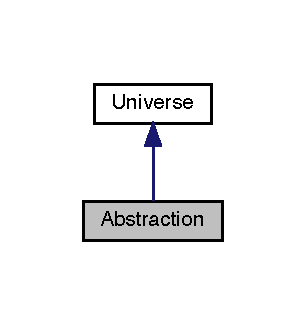
\includegraphics[width=147pt]{class_abstraction__inherit__graph}
\end{center}
\end{figure}


Collaboration diagram for Abstraction\+:
\nopagebreak
\begin{figure}[H]
\begin{center}
\leavevmode
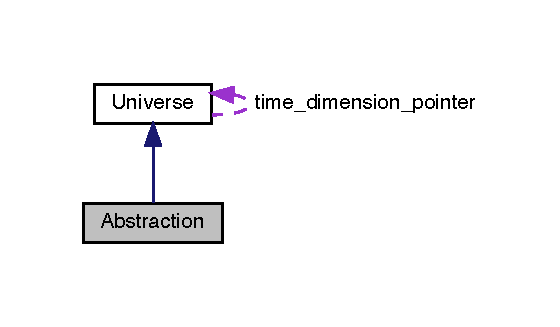
\includegraphics[width=269pt]{class_abstraction__coll__graph}
\end{center}
\end{figure}
\subsection*{Public Member Functions}
\begin{DoxyCompactItemize}
\item 
\hyperlink{class_abstraction_af4bf8b0e2bfd07d50ffc28b98f35b2ee}{Abstraction} ()
\item 
virtual \hyperlink{class_abstraction_aaf7d34417ea08792cc2b9449f9bfdc8e}{$\sim$\+Abstraction} ()
\item 
unsigned int \hyperlink{class_abstraction_a2b5e781d95a843a67db307b431f419a7}{Get\+Counter} (std\+::chrono\+::time\+\_\+point$<$ \hyperlink{universe_8h_a0ef8d951d1ca5ab3cfaf7ab4c7a6fd80}{Clock} $>$ event\+\_\+time)
\item 
void \hyperlink{class_abstraction_a82cd32bf3de41f35ab76d80611fe6763}{Set\+Counter} (std\+::chrono\+::time\+\_\+point$<$ \hyperlink{universe_8h_a0ef8d951d1ca5ab3cfaf7ab4c7a6fd80}{Clock} $>$ event\+\_\+time, unsigned int val)
\end{DoxyCompactItemize}
\subsection*{Additional Inherited Members}


\subsection{Detailed Description}


Definition at line 23 of file abstraction.\+h.



\subsection{Constructor \& Destructor Documentation}
\mbox{\Hypertarget{class_abstraction_af4bf8b0e2bfd07d50ffc28b98f35b2ee}\label{class_abstraction_af4bf8b0e2bfd07d50ffc28b98f35b2ee}} 
\index{Abstraction@{Abstraction}!Abstraction@{Abstraction}}
\index{Abstraction@{Abstraction}!Abstraction@{Abstraction}}
\subsubsection{\texorpdfstring{Abstraction()}{Abstraction()}}
{\footnotesize\ttfamily Abstraction\+::\+Abstraction (\begin{DoxyParamCaption}{ }\end{DoxyParamCaption})}

Default constructor \mbox{\Hypertarget{class_abstraction_aaf7d34417ea08792cc2b9449f9bfdc8e}\label{class_abstraction_aaf7d34417ea08792cc2b9449f9bfdc8e}} 
\index{Abstraction@{Abstraction}!````~Abstraction@{$\sim$\+Abstraction}}
\index{````~Abstraction@{$\sim$\+Abstraction}!Abstraction@{Abstraction}}
\subsubsection{\texorpdfstring{$\sim$\+Abstraction()}{~Abstraction()}}
{\footnotesize\ttfamily virtual Abstraction\+::$\sim$\+Abstraction (\begin{DoxyParamCaption}{ }\end{DoxyParamCaption})\hspace{0.3cm}{\ttfamily [virtual]}}

Default destructor 

\subsection{Member Function Documentation}
\mbox{\Hypertarget{class_abstraction_a2b5e781d95a843a67db307b431f419a7}\label{class_abstraction_a2b5e781d95a843a67db307b431f419a7}} 
\index{Abstraction@{Abstraction}!Get\+Counter@{Get\+Counter}}
\index{Get\+Counter@{Get\+Counter}!Abstraction@{Abstraction}}
\subsubsection{\texorpdfstring{Get\+Counter()}{GetCounter()}}
{\footnotesize\ttfamily unsigned int Abstraction\+::\+Get\+Counter (\begin{DoxyParamCaption}\item[{std\+::chrono\+::time\+\_\+point$<$ \hyperlink{universe_8h_a0ef8d951d1ca5ab3cfaf7ab4c7a6fd80}{Clock} $>$}]{event\+\_\+time }\end{DoxyParamCaption})\hspace{0.3cm}{\ttfamily [inline]}}

Access m\+\_\+\+Counter \begin{DoxyReturn}{Returns}
The current value of m\+\_\+\+Counter 
\end{DoxyReturn}


Definition at line 33 of file abstraction.\+h.

\mbox{\Hypertarget{class_abstraction_a82cd32bf3de41f35ab76d80611fe6763}\label{class_abstraction_a82cd32bf3de41f35ab76d80611fe6763}} 
\index{Abstraction@{Abstraction}!Set\+Counter@{Set\+Counter}}
\index{Set\+Counter@{Set\+Counter}!Abstraction@{Abstraction}}
\subsubsection{\texorpdfstring{Set\+Counter()}{SetCounter()}}
{\footnotesize\ttfamily void Abstraction\+::\+Set\+Counter (\begin{DoxyParamCaption}\item[{std\+::chrono\+::time\+\_\+point$<$ \hyperlink{universe_8h_a0ef8d951d1ca5ab3cfaf7ab4c7a6fd80}{Clock} $>$}]{event\+\_\+time,  }\item[{unsigned int}]{val }\end{DoxyParamCaption})\hspace{0.3cm}{\ttfamily [inline]}, {\ttfamily [virtual]}}

Set m\+\_\+\+Counter 
\begin{DoxyParams}{Parameters}
{\em val} & New value to Set \\
\hline
\end{DoxyParams}


Reimplemented from \hyperlink{class_universe_aa22202ae740eb1355529afcb13285e91}{Universe}.



Definition at line 37 of file abstraction.\+h.



The documentation for this class was generated from the following file\+:\begin{DoxyCompactItemize}
\item 
Brain\+Harmonics/\hyperlink{abstraction_8h}{abstraction.\+h}\end{DoxyCompactItemize}

\hypertarget{class_app_timer}{}\section{App\+Timer Class Reference}
\label{class_app_timer}\index{App\+Timer@{App\+Timer}}


{\ttfamily \#include $<$apptimer.\+h$>$}



Inheritance diagram for App\+Timer\+:\nopagebreak
\begin{figure}[H]
\begin{center}
\leavevmode
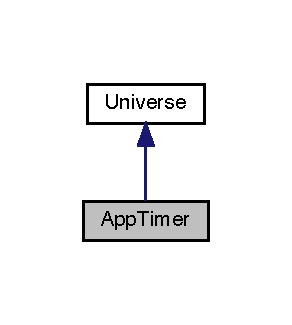
\includegraphics[width=140pt]{class_app_timer__inherit__graph}
\end{center}
\end{figure}


Collaboration diagram for App\+Timer\+:
\nopagebreak
\begin{figure}[H]
\begin{center}
\leavevmode
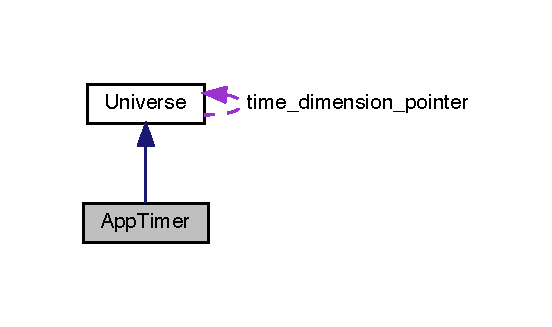
\includegraphics[width=265pt]{class_app_timer__coll__graph}
\end{center}
\end{figure}
\subsection*{Public Member Functions}
\begin{DoxyCompactItemize}
\item 
\hyperlink{class_app_timer_a59bf4eccdc9a3e16745b2cf9a122f935}{App\+Timer} ()
\item 
\hyperlink{class_app_timer_a06df15e33135f60f661c231e067951f3}{App\+Timer} (unsigned int object\+\_\+type)
\item 
\hyperlink{class_app_timer_a192075895ca575e9acb2663f3ebcecd6}{App\+Timer} (unsigned int object\+\_\+type, std\+::chrono\+::time\+\_\+point$<$ \hyperlink{universe_8h_a0ef8d951d1ca5ab3cfaf7ab4c7a6fd80}{Clock} $>$ event\+\_\+time)
\item 
\hyperlink{class_app_timer_af0836d131aa78b6812930199a5c7f9bd}{App\+Timer} (unsigned int object\+\_\+type, std\+::chrono\+::time\+\_\+point$<$ \hyperlink{universe_8h_a0ef8d951d1ca5ab3cfaf7ab4c7a6fd80}{Clock} $>$ event\+\_\+time, \hyperlink{class_universe}{Universe} \&universe\+\_\+connector)
\item 
virtual \hyperlink{class_app_timer_a5ef0c072a0591cf5a3bcc07edbd3577f}{$\sim$\+App\+Timer} ()
\item 
unsigned int \hyperlink{class_app_timer_ab9bb2b5f283b02d6d2292e064ddbd2ab}{Get\+Counter} (std\+::chrono\+::time\+\_\+point$<$ \hyperlink{universe_8h_a0ef8d951d1ca5ab3cfaf7ab4c7a6fd80}{Clock} $>$ event\+\_\+time)
\item 
void \hyperlink{class_app_timer_a77d5d447d6b136a35304b0571a166ddc}{Set\+Counter} (std\+::chrono\+::time\+\_\+point$<$ \hyperlink{universe_8h_a0ef8d951d1ca5ab3cfaf7ab4c7a6fd80}{Clock} $>$ event\+\_\+time, unsigned int val)
\end{DoxyCompactItemize}
\subsection*{Additional Inherited Members}


\subsection{Detailed Description}


Definition at line 23 of file apptimer.\+h.



\subsection{Constructor \& Destructor Documentation}
\mbox{\Hypertarget{class_app_timer_a59bf4eccdc9a3e16745b2cf9a122f935}\label{class_app_timer_a59bf4eccdc9a3e16745b2cf9a122f935}} 
\index{App\+Timer@{App\+Timer}!App\+Timer@{App\+Timer}}
\index{App\+Timer@{App\+Timer}!App\+Timer@{App\+Timer}}
\subsubsection{\texorpdfstring{App\+Timer()}{AppTimer()}\hspace{0.1cm}{\footnotesize\ttfamily [1/4]}}
{\footnotesize\ttfamily App\+Timer\+::\+App\+Timer (\begin{DoxyParamCaption}{ }\end{DoxyParamCaption})\hspace{0.3cm}{\ttfamily [inline]}}



Definition at line 26 of file apptimer.\+h.

\mbox{\Hypertarget{class_app_timer_a06df15e33135f60f661c231e067951f3}\label{class_app_timer_a06df15e33135f60f661c231e067951f3}} 
\index{App\+Timer@{App\+Timer}!App\+Timer@{App\+Timer}}
\index{App\+Timer@{App\+Timer}!App\+Timer@{App\+Timer}}
\subsubsection{\texorpdfstring{App\+Timer()}{AppTimer()}\hspace{0.1cm}{\footnotesize\ttfamily [2/4]}}
{\footnotesize\ttfamily App\+Timer\+::\+App\+Timer (\begin{DoxyParamCaption}\item[{unsigned int}]{object\+\_\+type }\end{DoxyParamCaption})\hspace{0.3cm}{\ttfamily [inline]}}



Definition at line 28 of file apptimer.\+h.

\mbox{\Hypertarget{class_app_timer_a192075895ca575e9acb2663f3ebcecd6}\label{class_app_timer_a192075895ca575e9acb2663f3ebcecd6}} 
\index{App\+Timer@{App\+Timer}!App\+Timer@{App\+Timer}}
\index{App\+Timer@{App\+Timer}!App\+Timer@{App\+Timer}}
\subsubsection{\texorpdfstring{App\+Timer()}{AppTimer()}\hspace{0.1cm}{\footnotesize\ttfamily [3/4]}}
{\footnotesize\ttfamily App\+Timer\+::\+App\+Timer (\begin{DoxyParamCaption}\item[{unsigned int}]{object\+\_\+type,  }\item[{std\+::chrono\+::time\+\_\+point$<$ \hyperlink{universe_8h_a0ef8d951d1ca5ab3cfaf7ab4c7a6fd80}{Clock} $>$}]{event\+\_\+time }\end{DoxyParamCaption})\hspace{0.3cm}{\ttfamily [inline]}}



Definition at line 30 of file apptimer.\+h.

\mbox{\Hypertarget{class_app_timer_af0836d131aa78b6812930199a5c7f9bd}\label{class_app_timer_af0836d131aa78b6812930199a5c7f9bd}} 
\index{App\+Timer@{App\+Timer}!App\+Timer@{App\+Timer}}
\index{App\+Timer@{App\+Timer}!App\+Timer@{App\+Timer}}
\subsubsection{\texorpdfstring{App\+Timer()}{AppTimer()}\hspace{0.1cm}{\footnotesize\ttfamily [4/4]}}
{\footnotesize\ttfamily App\+Timer\+::\+App\+Timer (\begin{DoxyParamCaption}\item[{unsigned int}]{object\+\_\+type,  }\item[{std\+::chrono\+::time\+\_\+point$<$ \hyperlink{universe_8h_a0ef8d951d1ca5ab3cfaf7ab4c7a6fd80}{Clock} $>$}]{event\+\_\+time,  }\item[{\hyperlink{class_universe}{Universe} \&}]{universe\+\_\+connector }\end{DoxyParamCaption})\hspace{0.3cm}{\ttfamily [inline]}}



Definition at line 32 of file apptimer.\+h.

Here is the call graph for this function\+:
\nopagebreak
\begin{figure}[H]
\begin{center}
\leavevmode
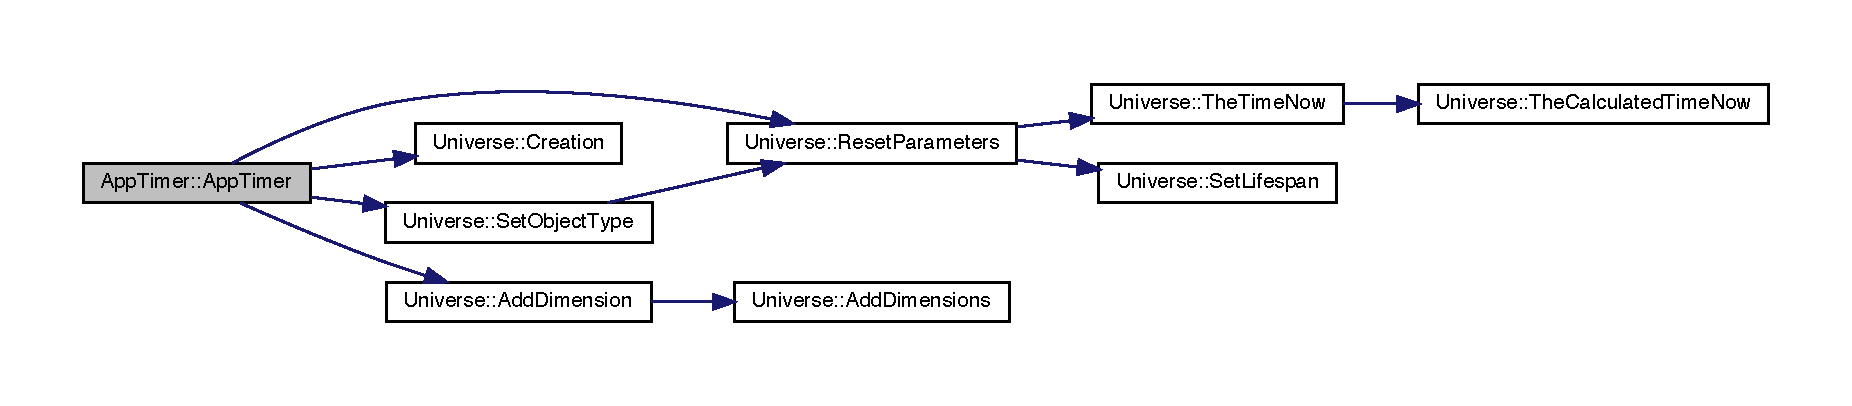
\includegraphics[width=350pt]{class_app_timer_af0836d131aa78b6812930199a5c7f9bd_cgraph}
\end{center}
\end{figure}
\mbox{\Hypertarget{class_app_timer_a5ef0c072a0591cf5a3bcc07edbd3577f}\label{class_app_timer_a5ef0c072a0591cf5a3bcc07edbd3577f}} 
\index{App\+Timer@{App\+Timer}!````~App\+Timer@{$\sim$\+App\+Timer}}
\index{````~App\+Timer@{$\sim$\+App\+Timer}!App\+Timer@{App\+Timer}}
\subsubsection{\texorpdfstring{$\sim$\+App\+Timer()}{~AppTimer()}}
{\footnotesize\ttfamily virtual App\+Timer\+::$\sim$\+App\+Timer (\begin{DoxyParamCaption}{ }\end{DoxyParamCaption})\hspace{0.3cm}{\ttfamily [inline]}, {\ttfamily [virtual]}}

Default destructor 

Definition at line 49 of file apptimer.\+h.



\subsection{Member Function Documentation}
\mbox{\Hypertarget{class_app_timer_ab9bb2b5f283b02d6d2292e064ddbd2ab}\label{class_app_timer_ab9bb2b5f283b02d6d2292e064ddbd2ab}} 
\index{App\+Timer@{App\+Timer}!Get\+Counter@{Get\+Counter}}
\index{Get\+Counter@{Get\+Counter}!App\+Timer@{App\+Timer}}
\subsubsection{\texorpdfstring{Get\+Counter()}{GetCounter()}}
{\footnotesize\ttfamily unsigned int App\+Timer\+::\+Get\+Counter (\begin{DoxyParamCaption}\item[{std\+::chrono\+::time\+\_\+point$<$ \hyperlink{universe_8h_a0ef8d951d1ca5ab3cfaf7ab4c7a6fd80}{Clock} $>$}]{event\+\_\+time }\end{DoxyParamCaption})\hspace{0.3cm}{\ttfamily [inline]}}



Definition at line 50 of file apptimer.\+h.

\mbox{\Hypertarget{class_app_timer_a77d5d447d6b136a35304b0571a166ddc}\label{class_app_timer_a77d5d447d6b136a35304b0571a166ddc}} 
\index{App\+Timer@{App\+Timer}!Set\+Counter@{Set\+Counter}}
\index{Set\+Counter@{Set\+Counter}!App\+Timer@{App\+Timer}}
\subsubsection{\texorpdfstring{Set\+Counter()}{SetCounter()}}
{\footnotesize\ttfamily void App\+Timer\+::\+Set\+Counter (\begin{DoxyParamCaption}\item[{std\+::chrono\+::time\+\_\+point$<$ \hyperlink{universe_8h_a0ef8d951d1ca5ab3cfaf7ab4c7a6fd80}{Clock} $>$}]{event\+\_\+time,  }\item[{unsigned int}]{val }\end{DoxyParamCaption})\hspace{0.3cm}{\ttfamily [inline]}, {\ttfamily [virtual]}}



Reimplemented from \hyperlink{class_universe_aa22202ae740eb1355529afcb13285e91}{Universe}.



Definition at line 51 of file apptimer.\+h.



The documentation for this class was generated from the following file\+:\begin{DoxyCompactItemize}
\item 
Brain\+Harmonics/\hyperlink{apptimer_8h}{apptimer.\+h}\end{DoxyCompactItemize}

\hypertarget{class_axon}{}\section{Axon Class Reference}
\label{class_axon}\index{Axon@{Axon}}


{\ttfamily \#include $<$axon.\+h$>$}



Inheritance diagram for Axon\+:\nopagebreak
\begin{figure}[H]
\begin{center}
\leavevmode
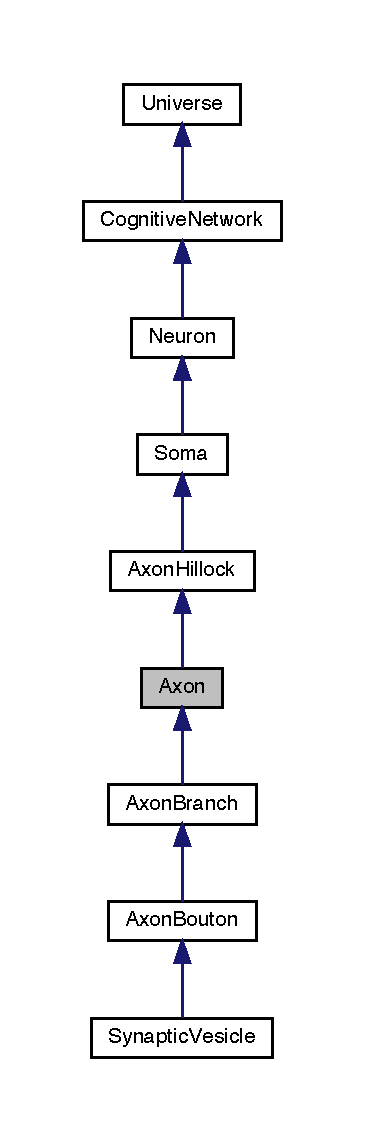
\includegraphics[width=175pt]{class_axon__inherit__graph}
\end{center}
\end{figure}


Collaboration diagram for Axon\+:\nopagebreak
\begin{figure}[H]
\begin{center}
\leavevmode
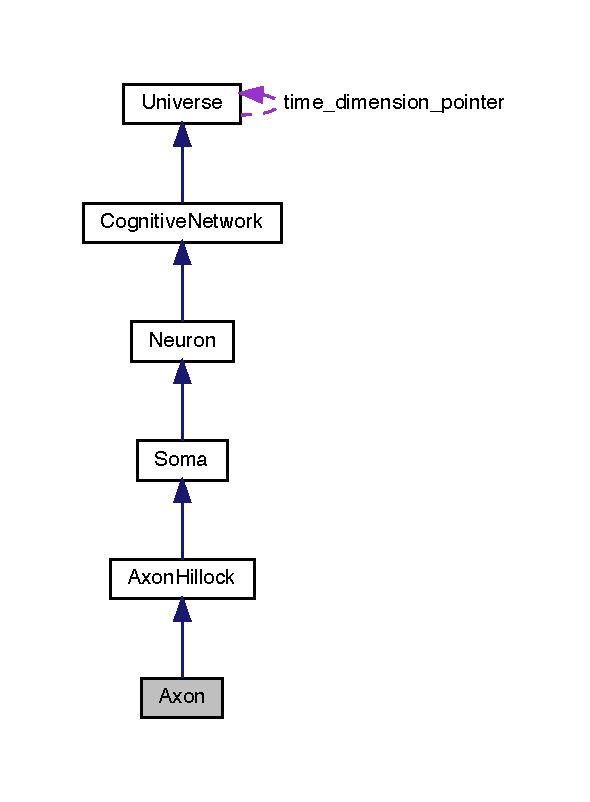
\includegraphics[width=283pt]{class_axon__coll__graph}
\end{center}
\end{figure}
\subsection*{Public Member Functions}
\begin{DoxyCompactItemize}
\item 
\mbox{\hyperlink{class_axon_a1a0703b026b74c83e418613d929c5d22}{Axon}} ()
\item 
\mbox{\hyperlink{class_axon_a7cc05238af77735983111d1ca58c9c9b}{Axon}} (unsigned int object\+\_\+type)
\item 
\mbox{\hyperlink{class_axon_a0ca4cd87ad4a2719c6b7c8c3d46dcbc6}{Axon}} (unsigned int object\+\_\+type, std\+::chrono\+::time\+\_\+point$<$ \mbox{\hyperlink{universe_8h_a0ef8d951d1ca5ab3cfaf7ab4c7a6fd80}{Clock}} $>$ event\+\_\+time)
\item 
\mbox{\hyperlink{class_axon_afaffed720efb3cb75e46088c5fb81d95}{Axon}} (unsigned int object\+\_\+type, std\+::chrono\+::time\+\_\+point$<$ \mbox{\hyperlink{universe_8h_a0ef8d951d1ca5ab3cfaf7ab4c7a6fd80}{Clock}} $>$ event\+\_\+time, \mbox{\hyperlink{class_axon_hillock}{Axon\+Hillock}} \&axonhillock\+\_\+connector)
\item 
virtual \mbox{\hyperlink{class_axon_af000507f0ff0527d1743e90d2e756282}{$\sim$\+Axon}} ()
\item 
unsigned int \mbox{\hyperlink{class_axon_a390ff1f3d85034fc85bcafc7374da9c7}{Get\+Counter}} (std\+::chrono\+::time\+\_\+point$<$ \mbox{\hyperlink{universe_8h_a0ef8d951d1ca5ab3cfaf7ab4c7a6fd80}{Clock}} $>$ event\+\_\+time)
\item 
double \mbox{\hyperlink{class_axon_a37a1ca2b0454d77dc0bc93e493feb0ce}{Get\+Energy}} (std\+::chrono\+::time\+\_\+point$<$ \mbox{\hyperlink{universe_8h_a0ef8d951d1ca5ab3cfaf7ab4c7a6fd80}{Clock}} $>$ event\+\_\+time)
\item 
\mbox{\hyperlink{glad_8h_a950fc91edb4504f62f1c577bf4727c29}{void}} \mbox{\hyperlink{class_axon_a3493cb97bde26bd66facc6084cd5f219}{Set\+Counter}} (std\+::chrono\+::time\+\_\+point$<$ \mbox{\hyperlink{universe_8h_a0ef8d951d1ca5ab3cfaf7ab4c7a6fd80}{Clock}} $>$ event\+\_\+time, unsigned int \mbox{\hyperlink{glad_8h_a26942fd2ed566ef553eae82d2c109c8f}{val}})
\item 
\mbox{\hyperlink{glad_8h_a950fc91edb4504f62f1c577bf4727c29}{void}} \mbox{\hyperlink{class_axon_af5108f451de97deb56138e8e81ced359}{Set\+Energy}} (std\+::chrono\+::time\+\_\+point$<$ \mbox{\hyperlink{universe_8h_a0ef8d951d1ca5ab3cfaf7ab4c7a6fd80}{Clock}} $>$ event\+\_\+time, double \mbox{\hyperlink{glad_8h_a26942fd2ed566ef553eae82d2c109c8f}{val}})
\item 
bool \mbox{\hyperlink{class_axon_ae079e0b47f5027625da158930e4fa9c5}{Reset\+Parameters}} (std\+::chrono\+::time\+\_\+point$<$ \mbox{\hyperlink{universe_8h_a0ef8d951d1ca5ab3cfaf7ab4c7a6fd80}{Clock}} $>$ event\+\_\+time)
\item 
\mbox{\hyperlink{class_axon}{Axon}} $\ast$ \mbox{\hyperlink{class_axon_a41e97ead4c793003db2de87061574c26}{Create\+Axon\+Branch}} (std\+::chrono\+::time\+\_\+point$<$ \mbox{\hyperlink{universe_8h_a0ef8d951d1ca5ab3cfaf7ab4c7a6fd80}{Clock}} $>$ event\+\_\+time)
\item 
std\+::vector$<$ \mbox{\hyperlink{class_axon}{Axon}} $\ast$ $>$ \mbox{\hyperlink{class_axon_ab0da51c05a0879efdb45c594b68ef8fd}{Create\+Axon\+Branches}} (std\+::chrono\+::time\+\_\+point$<$ \mbox{\hyperlink{universe_8h_a0ef8d951d1ca5ab3cfaf7ab4c7a6fd80}{Clock}} $>$ event\+\_\+time, int quantity)
\item 
\mbox{\hyperlink{class_axon}{Axon}} $\ast$ \mbox{\hyperlink{class_axon_a7720ee66a75e87f4e308b82d1841443a}{Clone\+Axon\+Branch}} (std\+::chrono\+::time\+\_\+point$<$ \mbox{\hyperlink{universe_8h_a0ef8d951d1ca5ab3cfaf7ab4c7a6fd80}{Clock}} $>$ event\+\_\+time, \mbox{\hyperlink{class_axon}{Axon}} $\ast$clone\+\_\+object, double perfection\+\_\+membership)
\item 
std\+::vector$<$ \mbox{\hyperlink{class_axon}{Axon}} $\ast$ $>$ \mbox{\hyperlink{class_axon_af2d6d5bc9ee0cd8ff654a949ef1cc294}{Clone\+Axon\+Branches}} (std\+::chrono\+::time\+\_\+point$<$ \mbox{\hyperlink{universe_8h_a0ef8d951d1ca5ab3cfaf7ab4c7a6fd80}{Clock}} $>$ event\+\_\+time, std\+::vector$<$ \mbox{\hyperlink{class_axon}{Axon}} $\ast$$>$ cloning\+\_\+list, double perfection\+\_\+membership)
\item 
\mbox{\hyperlink{class_axon}{Axon}} $\ast$ \mbox{\hyperlink{class_axon_a6ac580e4565d24c955b0a48d7a8b20e2}{Destroy\+Axon\+Branch}} (std\+::chrono\+::time\+\_\+point$<$ \mbox{\hyperlink{universe_8h_a0ef8d951d1ca5ab3cfaf7ab4c7a6fd80}{Clock}} $>$ event\+\_\+time, \mbox{\hyperlink{class_axon}{Axon}} $\ast$destroy\+\_\+object)
\item 
std\+::vector$<$ \mbox{\hyperlink{class_axon}{Axon}} $\ast$ $>$ \mbox{\hyperlink{class_axon_aa9d26eed8d178527d1995adfad2f67ac}{Destroy\+Axon\+Branches}} (std\+::chrono\+::time\+\_\+point$<$ \mbox{\hyperlink{universe_8h_a0ef8d951d1ca5ab3cfaf7ab4c7a6fd80}{Clock}} $>$ event\+\_\+time, std\+::vector$<$ \mbox{\hyperlink{class_axon}{Axon}} $\ast$$>$ destruction\+\_\+list)
\item 
\mbox{\hyperlink{class_axon}{Axon}} $\ast$ \mbox{\hyperlink{class_axon_a6ed85466115dab46ef71f26a420249ff}{Add\+Axon\+Branch}} (std\+::chrono\+::time\+\_\+point$<$ \mbox{\hyperlink{universe_8h_a0ef8d951d1ca5ab3cfaf7ab4c7a6fd80}{Clock}} $>$ event\+\_\+time, \mbox{\hyperlink{class_axon}{Axon}} $\ast$add\+\_\+object)
\item 
std\+::vector$<$ \mbox{\hyperlink{class_axon}{Axon}} $\ast$ $>$ \mbox{\hyperlink{class_axon_a04969d98c3fbb671cba5daccacffc003}{Add\+Axon\+Branches}} (std\+::chrono\+::time\+\_\+point$<$ \mbox{\hyperlink{universe_8h_a0ef8d951d1ca5ab3cfaf7ab4c7a6fd80}{Clock}} $>$ event\+\_\+time, std\+::vector$<$ \mbox{\hyperlink{class_axon}{Axon}} $\ast$$>$ add\+\_\+objects)
\item 
\mbox{\hyperlink{class_axon}{Axon}} $\ast$ \mbox{\hyperlink{class_axon_a7b43ca7f5b696c72ac17a27fea3b2822}{Remove\+Axon\+Branch}} (std\+::chrono\+::time\+\_\+point$<$ \mbox{\hyperlink{universe_8h_a0ef8d951d1ca5ab3cfaf7ab4c7a6fd80}{Clock}} $>$ event\+\_\+time)
\item 
std\+::vector$<$ \mbox{\hyperlink{class_axon}{Axon}} $\ast$ $>$ \mbox{\hyperlink{class_axon_a4c7af6c0900ae766c55362bfbb827ce3}{Remove\+Axon\+Branches}} (std\+::chrono\+::time\+\_\+point$<$ \mbox{\hyperlink{universe_8h_a0ef8d951d1ca5ab3cfaf7ab4c7a6fd80}{Clock}} $>$ event\+\_\+time, int quantity)
\item 
\mbox{\hyperlink{class_axon}{Axon}} $\ast$ \mbox{\hyperlink{class_axon_a723b00504169712e47f7437111ad4ae3}{Get\+Axon\+Branch}} (std\+::chrono\+::time\+\_\+point$<$ \mbox{\hyperlink{universe_8h_a0ef8d951d1ca5ab3cfaf7ab4c7a6fd80}{Clock}} $>$ event\+\_\+time, int selector)
\item 
std\+::vector$<$ \mbox{\hyperlink{class_axon}{Axon}} $\ast$ $>$ \mbox{\hyperlink{class_axon_adf5796ef2f72ce56516b37e7e09e9d6c}{Get\+Axon\+Branches}} (std\+::chrono\+::time\+\_\+point$<$ \mbox{\hyperlink{universe_8h_a0ef8d951d1ca5ab3cfaf7ab4c7a6fd80}{Clock}} $>$ event\+\_\+time)
\item 
int \mbox{\hyperlink{class_axon_a0065c335bc57e0a75962bcbd91f35001}{Growth}} (std\+::chrono\+::time\+\_\+point$<$ \mbox{\hyperlink{universe_8h_a0ef8d951d1ca5ab3cfaf7ab4c7a6fd80}{Clock}} $>$ event\+\_\+time)
\item 
int \mbox{\hyperlink{class_axon_a472ee760a1727072afaff0035d1eedd9}{Update}} (std\+::chrono\+::time\+\_\+point$<$ \mbox{\hyperlink{universe_8h_a0ef8d951d1ca5ab3cfaf7ab4c7a6fd80}{Clock}} $>$ event\+\_\+time)
\end{DoxyCompactItemize}
\subsection*{Protected Attributes}
\begin{DoxyCompactItemize}
\item 
std\+::vector$<$ \mbox{\hyperlink{class_axon}{Axon}} $\ast$ $>$ \mbox{\hyperlink{class_axon_ab32c0e4335cc4da8fe1aace7c16a88bf}{axonbranch\+\_\+list}}
\end{DoxyCompactItemize}
\subsection*{Additional Inherited Members}


\subsection{Detailed Description}


Definition at line 14 of file axon.\+h.



\subsection{Constructor \& Destructor Documentation}
\mbox{\Hypertarget{class_axon_a1a0703b026b74c83e418613d929c5d22}\label{class_axon_a1a0703b026b74c83e418613d929c5d22}} 
\index{Axon@{Axon}!Axon@{Axon}}
\index{Axon@{Axon}!Axon@{Axon}}
\subsubsection{\texorpdfstring{Axon()}{Axon()}\hspace{0.1cm}{\footnotesize\ttfamily [1/4]}}
{\footnotesize\ttfamily Axon\+::\+Axon (\begin{DoxyParamCaption}{ }\end{DoxyParamCaption})\hspace{0.3cm}{\ttfamily [inline]}}



Definition at line 17 of file axon.\+h.

\mbox{\Hypertarget{class_axon_a7cc05238af77735983111d1ca58c9c9b}\label{class_axon_a7cc05238af77735983111d1ca58c9c9b}} 
\index{Axon@{Axon}!Axon@{Axon}}
\index{Axon@{Axon}!Axon@{Axon}}
\subsubsection{\texorpdfstring{Axon()}{Axon()}\hspace{0.1cm}{\footnotesize\ttfamily [2/4]}}
{\footnotesize\ttfamily Axon\+::\+Axon (\begin{DoxyParamCaption}\item[{unsigned int}]{object\+\_\+type }\end{DoxyParamCaption})\hspace{0.3cm}{\ttfamily [inline]}}



Definition at line 19 of file axon.\+h.

\mbox{\Hypertarget{class_axon_a0ca4cd87ad4a2719c6b7c8c3d46dcbc6}\label{class_axon_a0ca4cd87ad4a2719c6b7c8c3d46dcbc6}} 
\index{Axon@{Axon}!Axon@{Axon}}
\index{Axon@{Axon}!Axon@{Axon}}
\subsubsection{\texorpdfstring{Axon()}{Axon()}\hspace{0.1cm}{\footnotesize\ttfamily [3/4]}}
{\footnotesize\ttfamily Axon\+::\+Axon (\begin{DoxyParamCaption}\item[{unsigned int}]{object\+\_\+type,  }\item[{std\+::chrono\+::time\+\_\+point$<$ \mbox{\hyperlink{universe_8h_a0ef8d951d1ca5ab3cfaf7ab4c7a6fd80}{Clock}} $>$}]{event\+\_\+time }\end{DoxyParamCaption})\hspace{0.3cm}{\ttfamily [inline]}}



Definition at line 21 of file axon.\+h.

\mbox{\Hypertarget{class_axon_afaffed720efb3cb75e46088c5fb81d95}\label{class_axon_afaffed720efb3cb75e46088c5fb81d95}} 
\index{Axon@{Axon}!Axon@{Axon}}
\index{Axon@{Axon}!Axon@{Axon}}
\subsubsection{\texorpdfstring{Axon()}{Axon()}\hspace{0.1cm}{\footnotesize\ttfamily [4/4]}}
{\footnotesize\ttfamily Axon\+::\+Axon (\begin{DoxyParamCaption}\item[{unsigned int}]{object\+\_\+type,  }\item[{std\+::chrono\+::time\+\_\+point$<$ \mbox{\hyperlink{universe_8h_a0ef8d951d1ca5ab3cfaf7ab4c7a6fd80}{Clock}} $>$}]{event\+\_\+time,  }\item[{\mbox{\hyperlink{class_axon_hillock}{Axon\+Hillock}} \&}]{axonhillock\+\_\+connector }\end{DoxyParamCaption})\hspace{0.3cm}{\ttfamily [inline]}}



Definition at line 23 of file axon.\+h.

Here is the call graph for this function\+:\nopagebreak
\begin{figure}[H]
\begin{center}
\leavevmode
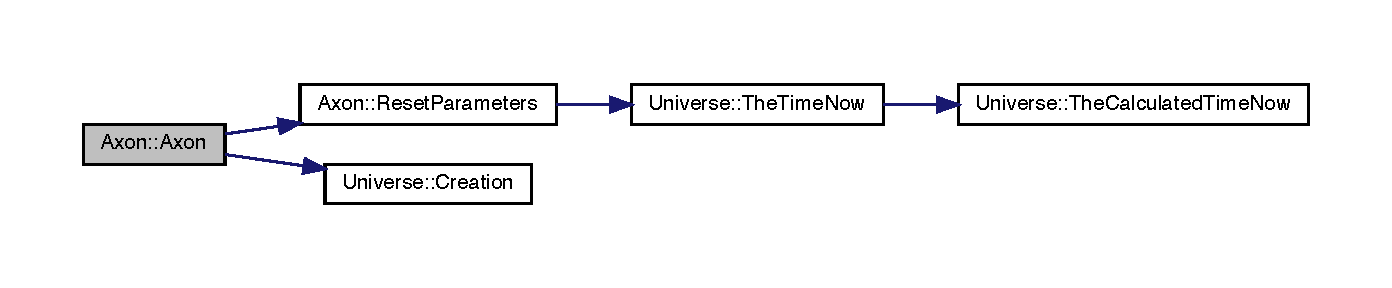
\includegraphics[width=350pt]{class_axon_afaffed720efb3cb75e46088c5fb81d95_cgraph}
\end{center}
\end{figure}
\mbox{\Hypertarget{class_axon_af000507f0ff0527d1743e90d2e756282}\label{class_axon_af000507f0ff0527d1743e90d2e756282}} 
\index{Axon@{Axon}!````~Axon@{$\sim$\+Axon}}
\index{````~Axon@{$\sim$\+Axon}!Axon@{Axon}}
\subsubsection{\texorpdfstring{$\sim$\+Axon()}{~Axon()}}
{\footnotesize\ttfamily virtual Axon\+::$\sim$\+Axon (\begin{DoxyParamCaption}{ }\end{DoxyParamCaption})\hspace{0.3cm}{\ttfamily [inline]}, {\ttfamily [virtual]}}

Default destructor 

Definition at line 36 of file axon.\+h.



\subsection{Member Function Documentation}
\mbox{\Hypertarget{class_axon_a6ed85466115dab46ef71f26a420249ff}\label{class_axon_a6ed85466115dab46ef71f26a420249ff}} 
\index{Axon@{Axon}!Add\+Axon\+Branch@{Add\+Axon\+Branch}}
\index{Add\+Axon\+Branch@{Add\+Axon\+Branch}!Axon@{Axon}}
\subsubsection{\texorpdfstring{Add\+Axon\+Branch()}{AddAxonBranch()}}
{\footnotesize\ttfamily \mbox{\hyperlink{class_axon}{Axon}} $\ast$ Axon\+::\+Add\+Axon\+Branch (\begin{DoxyParamCaption}\item[{std\+::chrono\+::time\+\_\+point$<$ \mbox{\hyperlink{universe_8h_a0ef8d951d1ca5ab3cfaf7ab4c7a6fd80}{Clock}} $>$}]{event\+\_\+time,  }\item[{\mbox{\hyperlink{class_axon}{Axon}} $\ast$}]{add\+\_\+object }\end{DoxyParamCaption})}



Definition at line 115 of file axon.\+cc.

Here is the caller graph for this function\+:\nopagebreak
\begin{figure}[H]
\begin{center}
\leavevmode
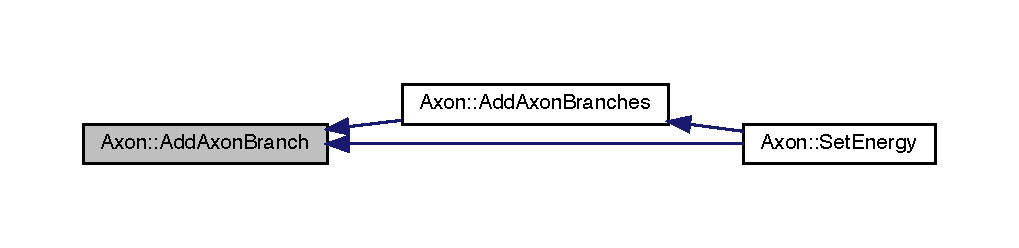
\includegraphics[width=350pt]{class_axon_a6ed85466115dab46ef71f26a420249ff_icgraph}
\end{center}
\end{figure}
\mbox{\Hypertarget{class_axon_a04969d98c3fbb671cba5daccacffc003}\label{class_axon_a04969d98c3fbb671cba5daccacffc003}} 
\index{Axon@{Axon}!Add\+Axon\+Branches@{Add\+Axon\+Branches}}
\index{Add\+Axon\+Branches@{Add\+Axon\+Branches}!Axon@{Axon}}
\subsubsection{\texorpdfstring{Add\+Axon\+Branches()}{AddAxonBranches()}}
{\footnotesize\ttfamily std\+::vector$<$ \mbox{\hyperlink{class_axon}{Axon}} $\ast$ $>$ Axon\+::\+Add\+Axon\+Branches (\begin{DoxyParamCaption}\item[{std\+::chrono\+::time\+\_\+point$<$ \mbox{\hyperlink{universe_8h_a0ef8d951d1ca5ab3cfaf7ab4c7a6fd80}{Clock}} $>$}]{event\+\_\+time,  }\item[{std\+::vector$<$ \mbox{\hyperlink{class_axon}{Axon}} $\ast$$>$}]{add\+\_\+objects }\end{DoxyParamCaption})}



Definition at line 126 of file axon.\+cc.

Here is the call graph for this function\+:\nopagebreak
\begin{figure}[H]
\begin{center}
\leavevmode
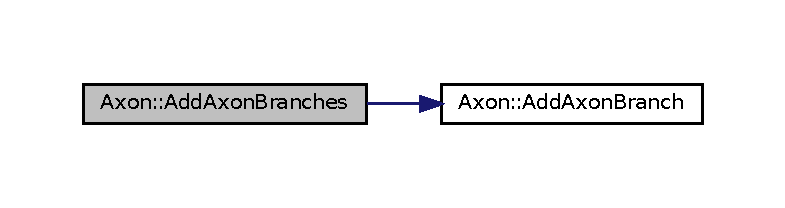
\includegraphics[width=350pt]{class_axon_a04969d98c3fbb671cba5daccacffc003_cgraph}
\end{center}
\end{figure}
\mbox{\Hypertarget{class_axon_a7720ee66a75e87f4e308b82d1841443a}\label{class_axon_a7720ee66a75e87f4e308b82d1841443a}} 
\index{Axon@{Axon}!Clone\+Axon\+Branch@{Clone\+Axon\+Branch}}
\index{Clone\+Axon\+Branch@{Clone\+Axon\+Branch}!Axon@{Axon}}
\subsubsection{\texorpdfstring{Clone\+Axon\+Branch()}{CloneAxonBranch()}}
{\footnotesize\ttfamily \mbox{\hyperlink{class_axon}{Axon}} $\ast$ Axon\+::\+Clone\+Axon\+Branch (\begin{DoxyParamCaption}\item[{std\+::chrono\+::time\+\_\+point$<$ \mbox{\hyperlink{universe_8h_a0ef8d951d1ca5ab3cfaf7ab4c7a6fd80}{Clock}} $>$}]{event\+\_\+time,  }\item[{\mbox{\hyperlink{class_axon}{Axon}} $\ast$}]{clone\+\_\+object,  }\item[{double}]{perfection\+\_\+membership }\end{DoxyParamCaption})}



Definition at line 100 of file axon.\+cc.

\mbox{\Hypertarget{class_axon_af2d6d5bc9ee0cd8ff654a949ef1cc294}\label{class_axon_af2d6d5bc9ee0cd8ff654a949ef1cc294}} 
\index{Axon@{Axon}!Clone\+Axon\+Branches@{Clone\+Axon\+Branches}}
\index{Clone\+Axon\+Branches@{Clone\+Axon\+Branches}!Axon@{Axon}}
\subsubsection{\texorpdfstring{Clone\+Axon\+Branches()}{CloneAxonBranches()}}
{\footnotesize\ttfamily std\+::vector$<$ \mbox{\hyperlink{class_axon}{Axon}} $\ast$ $>$ Axon\+::\+Clone\+Axon\+Branches (\begin{DoxyParamCaption}\item[{std\+::chrono\+::time\+\_\+point$<$ \mbox{\hyperlink{universe_8h_a0ef8d951d1ca5ab3cfaf7ab4c7a6fd80}{Clock}} $>$}]{event\+\_\+time,  }\item[{std\+::vector$<$ \mbox{\hyperlink{class_axon}{Axon}} $\ast$$>$}]{cloning\+\_\+list,  }\item[{double}]{perfection\+\_\+membership }\end{DoxyParamCaption})}



Definition at line 95 of file axon.\+cc.

\mbox{\Hypertarget{class_axon_a41e97ead4c793003db2de87061574c26}\label{class_axon_a41e97ead4c793003db2de87061574c26}} 
\index{Axon@{Axon}!Create\+Axon\+Branch@{Create\+Axon\+Branch}}
\index{Create\+Axon\+Branch@{Create\+Axon\+Branch}!Axon@{Axon}}
\subsubsection{\texorpdfstring{Create\+Axon\+Branch()}{CreateAxonBranch()}}
{\footnotesize\ttfamily \mbox{\hyperlink{class_axon}{Axon}} $\ast$ Axon\+::\+Create\+Axon\+Branch (\begin{DoxyParamCaption}\item[{std\+::chrono\+::time\+\_\+point$<$ \mbox{\hyperlink{universe_8h_a0ef8d951d1ca5ab3cfaf7ab4c7a6fd80}{Clock}} $>$}]{event\+\_\+time }\end{DoxyParamCaption})}



Definition at line 62 of file axon.\+cc.

Here is the caller graph for this function\+:\nopagebreak
\begin{figure}[H]
\begin{center}
\leavevmode
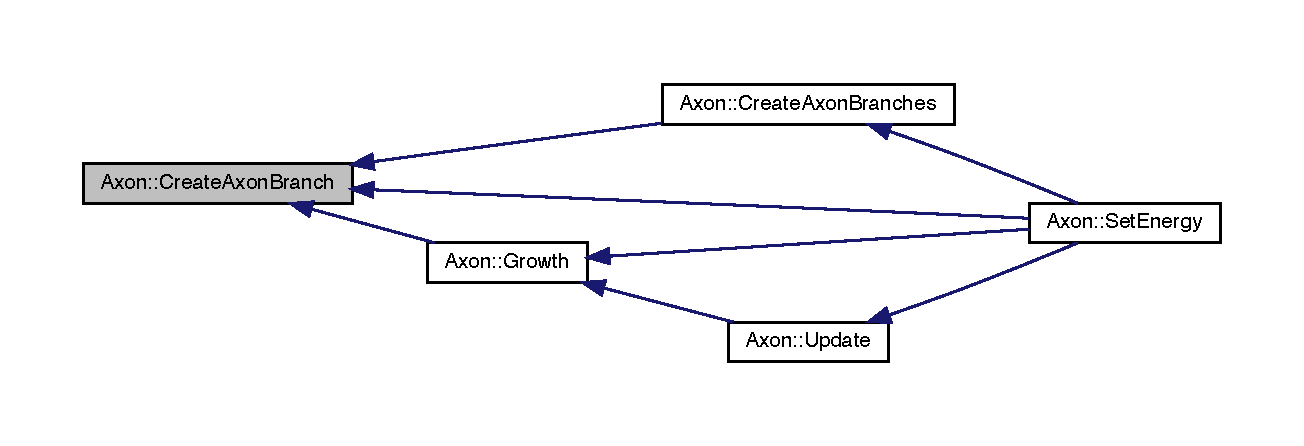
\includegraphics[width=350pt]{class_axon_a41e97ead4c793003db2de87061574c26_icgraph}
\end{center}
\end{figure}
\mbox{\Hypertarget{class_axon_ab0da51c05a0879efdb45c594b68ef8fd}\label{class_axon_ab0da51c05a0879efdb45c594b68ef8fd}} 
\index{Axon@{Axon}!Create\+Axon\+Branches@{Create\+Axon\+Branches}}
\index{Create\+Axon\+Branches@{Create\+Axon\+Branches}!Axon@{Axon}}
\subsubsection{\texorpdfstring{Create\+Axon\+Branches()}{CreateAxonBranches()}}
{\footnotesize\ttfamily std\+::vector$<$ \mbox{\hyperlink{class_axon}{Axon}} $\ast$ $>$ Axon\+::\+Create\+Axon\+Branches (\begin{DoxyParamCaption}\item[{std\+::chrono\+::time\+\_\+point$<$ \mbox{\hyperlink{universe_8h_a0ef8d951d1ca5ab3cfaf7ab4c7a6fd80}{Clock}} $>$}]{event\+\_\+time,  }\item[{int}]{quantity }\end{DoxyParamCaption})}



Definition at line 73 of file axon.\+cc.

Here is the call graph for this function\+:\nopagebreak
\begin{figure}[H]
\begin{center}
\leavevmode
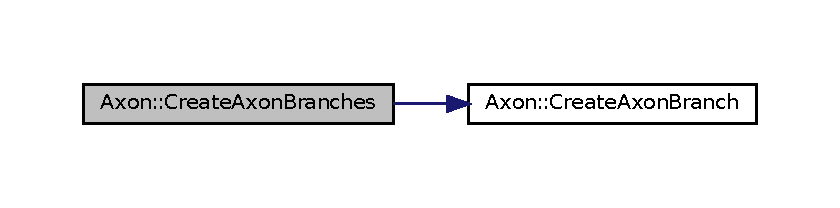
\includegraphics[width=350pt]{class_axon_ab0da51c05a0879efdb45c594b68ef8fd_cgraph}
\end{center}
\end{figure}
\mbox{\Hypertarget{class_axon_a6ac580e4565d24c955b0a48d7a8b20e2}\label{class_axon_a6ac580e4565d24c955b0a48d7a8b20e2}} 
\index{Axon@{Axon}!Destroy\+Axon\+Branch@{Destroy\+Axon\+Branch}}
\index{Destroy\+Axon\+Branch@{Destroy\+Axon\+Branch}!Axon@{Axon}}
\subsubsection{\texorpdfstring{Destroy\+Axon\+Branch()}{DestroyAxonBranch()}}
{\footnotesize\ttfamily \mbox{\hyperlink{class_axon}{Axon}} $\ast$ Axon\+::\+Destroy\+Axon\+Branch (\begin{DoxyParamCaption}\item[{std\+::chrono\+::time\+\_\+point$<$ \mbox{\hyperlink{universe_8h_a0ef8d951d1ca5ab3cfaf7ab4c7a6fd80}{Clock}} $>$}]{event\+\_\+time,  }\item[{\mbox{\hyperlink{class_axon}{Axon}} $\ast$}]{destroy\+\_\+object }\end{DoxyParamCaption})}



Definition at line 110 of file axon.\+cc.

\mbox{\Hypertarget{class_axon_aa9d26eed8d178527d1995adfad2f67ac}\label{class_axon_aa9d26eed8d178527d1995adfad2f67ac}} 
\index{Axon@{Axon}!Destroy\+Axon\+Branches@{Destroy\+Axon\+Branches}}
\index{Destroy\+Axon\+Branches@{Destroy\+Axon\+Branches}!Axon@{Axon}}
\subsubsection{\texorpdfstring{Destroy\+Axon\+Branches()}{DestroyAxonBranches()}}
{\footnotesize\ttfamily std\+::vector$<$ \mbox{\hyperlink{class_axon}{Axon}} $\ast$ $>$ Axon\+::\+Destroy\+Axon\+Branches (\begin{DoxyParamCaption}\item[{std\+::chrono\+::time\+\_\+point$<$ \mbox{\hyperlink{universe_8h_a0ef8d951d1ca5ab3cfaf7ab4c7a6fd80}{Clock}} $>$}]{event\+\_\+time,  }\item[{std\+::vector$<$ \mbox{\hyperlink{class_axon}{Axon}} $\ast$$>$}]{destruction\+\_\+list }\end{DoxyParamCaption})}



Definition at line 105 of file axon.\+cc.

\mbox{\Hypertarget{class_axon_a723b00504169712e47f7437111ad4ae3}\label{class_axon_a723b00504169712e47f7437111ad4ae3}} 
\index{Axon@{Axon}!Get\+Axon\+Branch@{Get\+Axon\+Branch}}
\index{Get\+Axon\+Branch@{Get\+Axon\+Branch}!Axon@{Axon}}
\subsubsection{\texorpdfstring{Get\+Axon\+Branch()}{GetAxonBranch()}}
{\footnotesize\ttfamily \mbox{\hyperlink{class_axon}{Axon}} $\ast$ Axon\+::\+Get\+Axon\+Branch (\begin{DoxyParamCaption}\item[{std\+::chrono\+::time\+\_\+point$<$ \mbox{\hyperlink{universe_8h_a0ef8d951d1ca5ab3cfaf7ab4c7a6fd80}{Clock}} $>$}]{event\+\_\+time,  }\item[{int}]{selector }\end{DoxyParamCaption})}



Definition at line 159 of file axon.\+cc.

\mbox{\Hypertarget{class_axon_adf5796ef2f72ce56516b37e7e09e9d6c}\label{class_axon_adf5796ef2f72ce56516b37e7e09e9d6c}} 
\index{Axon@{Axon}!Get\+Axon\+Branches@{Get\+Axon\+Branches}}
\index{Get\+Axon\+Branches@{Get\+Axon\+Branches}!Axon@{Axon}}
\subsubsection{\texorpdfstring{Get\+Axon\+Branches()}{GetAxonBranches()}}
{\footnotesize\ttfamily std\+::vector$<$ \mbox{\hyperlink{class_axon}{Axon}} $\ast$ $>$ Axon\+::\+Get\+Axon\+Branches (\begin{DoxyParamCaption}\item[{std\+::chrono\+::time\+\_\+point$<$ \mbox{\hyperlink{universe_8h_a0ef8d951d1ca5ab3cfaf7ab4c7a6fd80}{Clock}} $>$}]{event\+\_\+time }\end{DoxyParamCaption})}



Definition at line 164 of file axon.\+cc.

\mbox{\Hypertarget{class_axon_a390ff1f3d85034fc85bcafc7374da9c7}\label{class_axon_a390ff1f3d85034fc85bcafc7374da9c7}} 
\index{Axon@{Axon}!Get\+Counter@{Get\+Counter}}
\index{Get\+Counter@{Get\+Counter}!Axon@{Axon}}
\subsubsection{\texorpdfstring{Get\+Counter()}{GetCounter()}}
{\footnotesize\ttfamily unsigned int Axon\+::\+Get\+Counter (\begin{DoxyParamCaption}\item[{std\+::chrono\+::time\+\_\+point$<$ \mbox{\hyperlink{universe_8h_a0ef8d951d1ca5ab3cfaf7ab4c7a6fd80}{Clock}} $>$}]{event\+\_\+time }\end{DoxyParamCaption})\hspace{0.3cm}{\ttfamily [inline]}}

Access m\+\_\+\+Counter \begin{DoxyReturn}{Returns}
The current value of m\+\_\+\+Counter 
\end{DoxyReturn}


Definition at line 40 of file axon.\+h.

\mbox{\Hypertarget{class_axon_a37a1ca2b0454d77dc0bc93e493feb0ce}\label{class_axon_a37a1ca2b0454d77dc0bc93e493feb0ce}} 
\index{Axon@{Axon}!Get\+Energy@{Get\+Energy}}
\index{Get\+Energy@{Get\+Energy}!Axon@{Axon}}
\subsubsection{\texorpdfstring{Get\+Energy()}{GetEnergy()}}
{\footnotesize\ttfamily double Axon\+::\+Get\+Energy (\begin{DoxyParamCaption}\item[{std\+::chrono\+::time\+\_\+point$<$ \mbox{\hyperlink{universe_8h_a0ef8d951d1ca5ab3cfaf7ab4c7a6fd80}{Clock}} $>$}]{event\+\_\+time }\end{DoxyParamCaption})\hspace{0.3cm}{\ttfamily [inline]}}



Definition at line 41 of file axon.\+h.

\mbox{\Hypertarget{class_axon_a0065c335bc57e0a75962bcbd91f35001}\label{class_axon_a0065c335bc57e0a75962bcbd91f35001}} 
\index{Axon@{Axon}!Growth@{Growth}}
\index{Growth@{Growth}!Axon@{Axon}}
\subsubsection{\texorpdfstring{Growth()}{Growth()}}
{\footnotesize\ttfamily int Axon\+::\+Growth (\begin{DoxyParamCaption}\item[{std\+::chrono\+::time\+\_\+point$<$ \mbox{\hyperlink{universe_8h_a0ef8d951d1ca5ab3cfaf7ab4c7a6fd80}{Clock}} $>$}]{event\+\_\+time }\end{DoxyParamCaption})}



Definition at line 169 of file axon.\+cc.

Here is the call graph for this function\+:\nopagebreak
\begin{figure}[H]
\begin{center}
\leavevmode
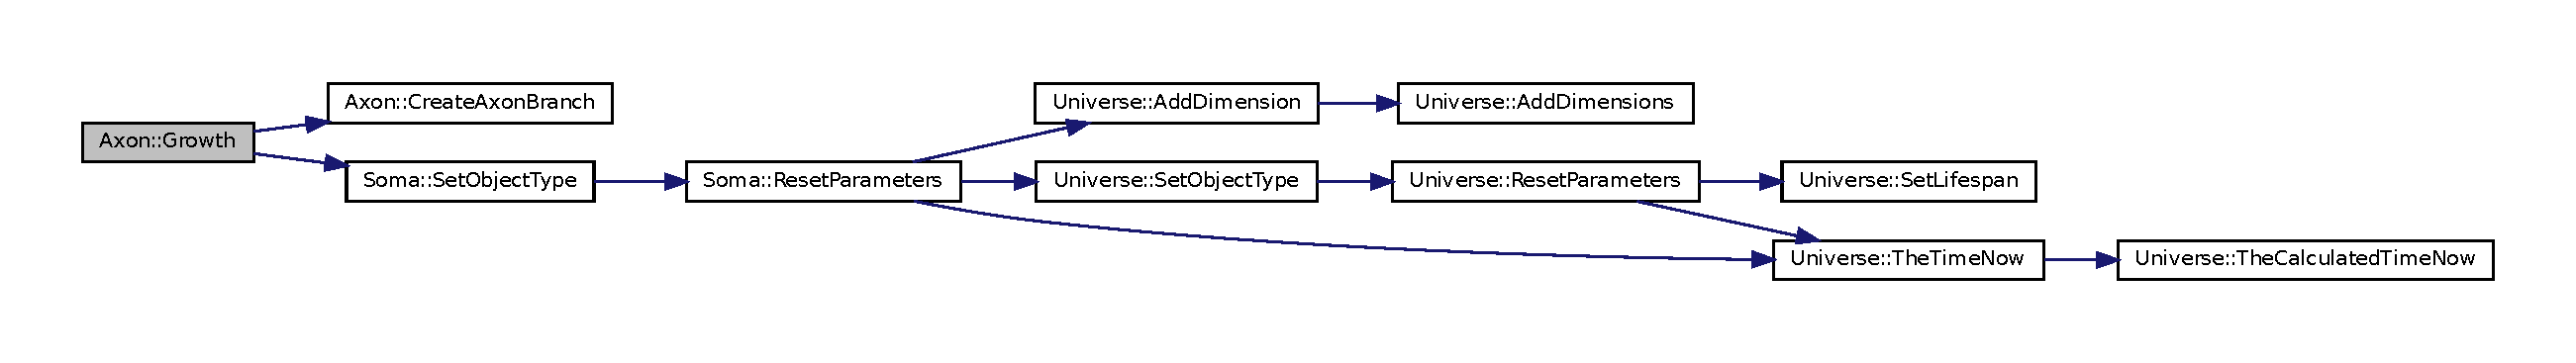
\includegraphics[width=350pt]{class_axon_a0065c335bc57e0a75962bcbd91f35001_cgraph}
\end{center}
\end{figure}
Here is the caller graph for this function\+:\nopagebreak
\begin{figure}[H]
\begin{center}
\leavevmode
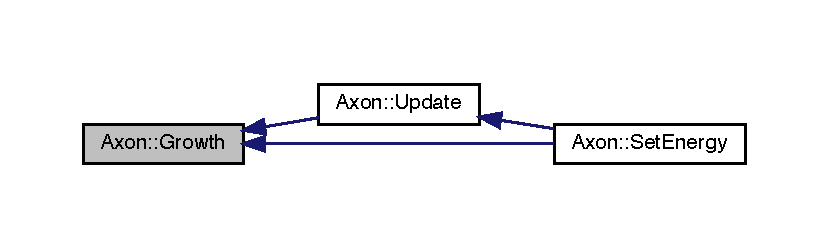
\includegraphics[width=282pt]{class_axon_a0065c335bc57e0a75962bcbd91f35001_icgraph}
\end{center}
\end{figure}
\mbox{\Hypertarget{class_axon_a7b43ca7f5b696c72ac17a27fea3b2822}\label{class_axon_a7b43ca7f5b696c72ac17a27fea3b2822}} 
\index{Axon@{Axon}!Remove\+Axon\+Branch@{Remove\+Axon\+Branch}}
\index{Remove\+Axon\+Branch@{Remove\+Axon\+Branch}!Axon@{Axon}}
\subsubsection{\texorpdfstring{Remove\+Axon\+Branch()}{RemoveAxonBranch()}}
{\footnotesize\ttfamily \mbox{\hyperlink{class_axon}{Axon}} $\ast$ Axon\+::\+Remove\+Axon\+Branch (\begin{DoxyParamCaption}\item[{std\+::chrono\+::time\+\_\+point$<$ \mbox{\hyperlink{universe_8h_a0ef8d951d1ca5ab3cfaf7ab4c7a6fd80}{Clock}} $>$}]{event\+\_\+time }\end{DoxyParamCaption})}



Definition at line 148 of file axon.\+cc.

\mbox{\Hypertarget{class_axon_a4c7af6c0900ae766c55362bfbb827ce3}\label{class_axon_a4c7af6c0900ae766c55362bfbb827ce3}} 
\index{Axon@{Axon}!Remove\+Axon\+Branches@{Remove\+Axon\+Branches}}
\index{Remove\+Axon\+Branches@{Remove\+Axon\+Branches}!Axon@{Axon}}
\subsubsection{\texorpdfstring{Remove\+Axon\+Branches()}{RemoveAxonBranches()}}
{\footnotesize\ttfamily std\+::vector$<$ \mbox{\hyperlink{class_axon}{Axon}} $\ast$ $>$ Axon\+::\+Remove\+Axon\+Branches (\begin{DoxyParamCaption}\item[{std\+::chrono\+::time\+\_\+point$<$ \mbox{\hyperlink{universe_8h_a0ef8d951d1ca5ab3cfaf7ab4c7a6fd80}{Clock}} $>$}]{event\+\_\+time,  }\item[{int}]{quantity }\end{DoxyParamCaption})}



Definition at line 154 of file axon.\+cc.

\mbox{\Hypertarget{class_axon_ae079e0b47f5027625da158930e4fa9c5}\label{class_axon_ae079e0b47f5027625da158930e4fa9c5}} 
\index{Axon@{Axon}!Reset\+Parameters@{Reset\+Parameters}}
\index{Reset\+Parameters@{Reset\+Parameters}!Axon@{Axon}}
\subsubsection{\texorpdfstring{Reset\+Parameters()}{ResetParameters()}}
{\footnotesize\ttfamily bool Axon\+::\+Reset\+Parameters (\begin{DoxyParamCaption}\item[{std\+::chrono\+::time\+\_\+point$<$ \mbox{\hyperlink{universe_8h_a0ef8d951d1ca5ab3cfaf7ab4c7a6fd80}{Clock}} $>$}]{event\+\_\+time }\end{DoxyParamCaption})}



Definition at line 20 of file axon.\+cc.

Here is the call graph for this function\+:\nopagebreak
\begin{figure}[H]
\begin{center}
\leavevmode
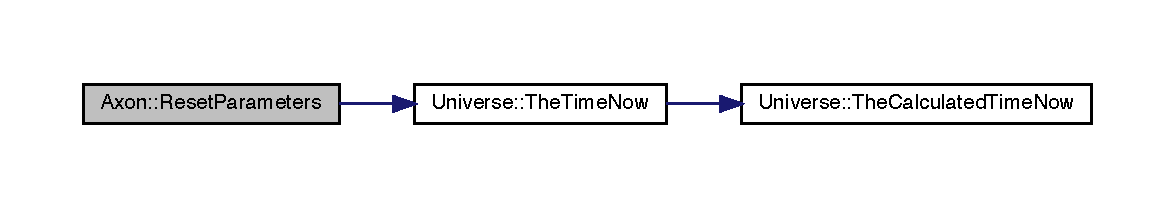
\includegraphics[width=350pt]{class_axon_ae079e0b47f5027625da158930e4fa9c5_cgraph}
\end{center}
\end{figure}
Here is the caller graph for this function\+:\nopagebreak
\begin{figure}[H]
\begin{center}
\leavevmode
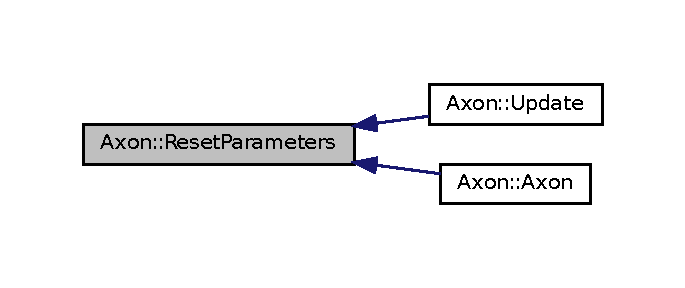
\includegraphics[width=329pt]{class_axon_ae079e0b47f5027625da158930e4fa9c5_icgraph}
\end{center}
\end{figure}
\mbox{\Hypertarget{class_axon_a3493cb97bde26bd66facc6084cd5f219}\label{class_axon_a3493cb97bde26bd66facc6084cd5f219}} 
\index{Axon@{Axon}!Set\+Counter@{Set\+Counter}}
\index{Set\+Counter@{Set\+Counter}!Axon@{Axon}}
\subsubsection{\texorpdfstring{Set\+Counter()}{SetCounter()}}
{\footnotesize\ttfamily \mbox{\hyperlink{glad_8h_a950fc91edb4504f62f1c577bf4727c29}{void}} Axon\+::\+Set\+Counter (\begin{DoxyParamCaption}\item[{std\+::chrono\+::time\+\_\+point$<$ \mbox{\hyperlink{universe_8h_a0ef8d951d1ca5ab3cfaf7ab4c7a6fd80}{Clock}} $>$}]{event\+\_\+time,  }\item[{unsigned int}]{val }\end{DoxyParamCaption})\hspace{0.3cm}{\ttfamily [inline]}, {\ttfamily [virtual]}}



Reimplemented from \mbox{\hyperlink{class_universe_aa22202ae740eb1355529afcb13285e91}{Universe}}.



Reimplemented in \mbox{\hyperlink{class_synaptic_vesicle_a7fd7cfce5eccb904206d968866f85220}{Synaptic\+Vesicle}}, \mbox{\hyperlink{class_axon_bouton_afe285478d414f2815afb98abe7b92898}{Axon\+Bouton}}, and \mbox{\hyperlink{class_axon_branch_a96ba30b18627563d637d4e02fac943be}{Axon\+Branch}}.



Definition at line 43 of file axon.\+h.

\mbox{\Hypertarget{class_axon_af5108f451de97deb56138e8e81ced359}\label{class_axon_af5108f451de97deb56138e8e81ced359}} 
\index{Axon@{Axon}!Set\+Energy@{Set\+Energy}}
\index{Set\+Energy@{Set\+Energy}!Axon@{Axon}}
\subsubsection{\texorpdfstring{Set\+Energy()}{SetEnergy()}}
{\footnotesize\ttfamily \mbox{\hyperlink{glad_8h_a950fc91edb4504f62f1c577bf4727c29}{void}} Axon\+::\+Set\+Energy (\begin{DoxyParamCaption}\item[{std\+::chrono\+::time\+\_\+point$<$ \mbox{\hyperlink{universe_8h_a0ef8d951d1ca5ab3cfaf7ab4c7a6fd80}{Clock}} $>$}]{event\+\_\+time,  }\item[{double}]{val }\end{DoxyParamCaption})\hspace{0.3cm}{\ttfamily [inline]}}



Definition at line 44 of file axon.\+h.

\mbox{\Hypertarget{class_axon_a472ee760a1727072afaff0035d1eedd9}\label{class_axon_a472ee760a1727072afaff0035d1eedd9}} 
\index{Axon@{Axon}!Update@{Update}}
\index{Update@{Update}!Axon@{Axon}}
\subsubsection{\texorpdfstring{Update()}{Update()}}
{\footnotesize\ttfamily int Axon\+::\+Update (\begin{DoxyParamCaption}\item[{std\+::chrono\+::time\+\_\+point$<$ \mbox{\hyperlink{universe_8h_a0ef8d951d1ca5ab3cfaf7ab4c7a6fd80}{Clock}} $>$}]{event\+\_\+time }\end{DoxyParamCaption})}



Definition at line 197 of file axon.\+cc.

Here is the call graph for this function\+:\nopagebreak
\begin{figure}[H]
\begin{center}
\leavevmode
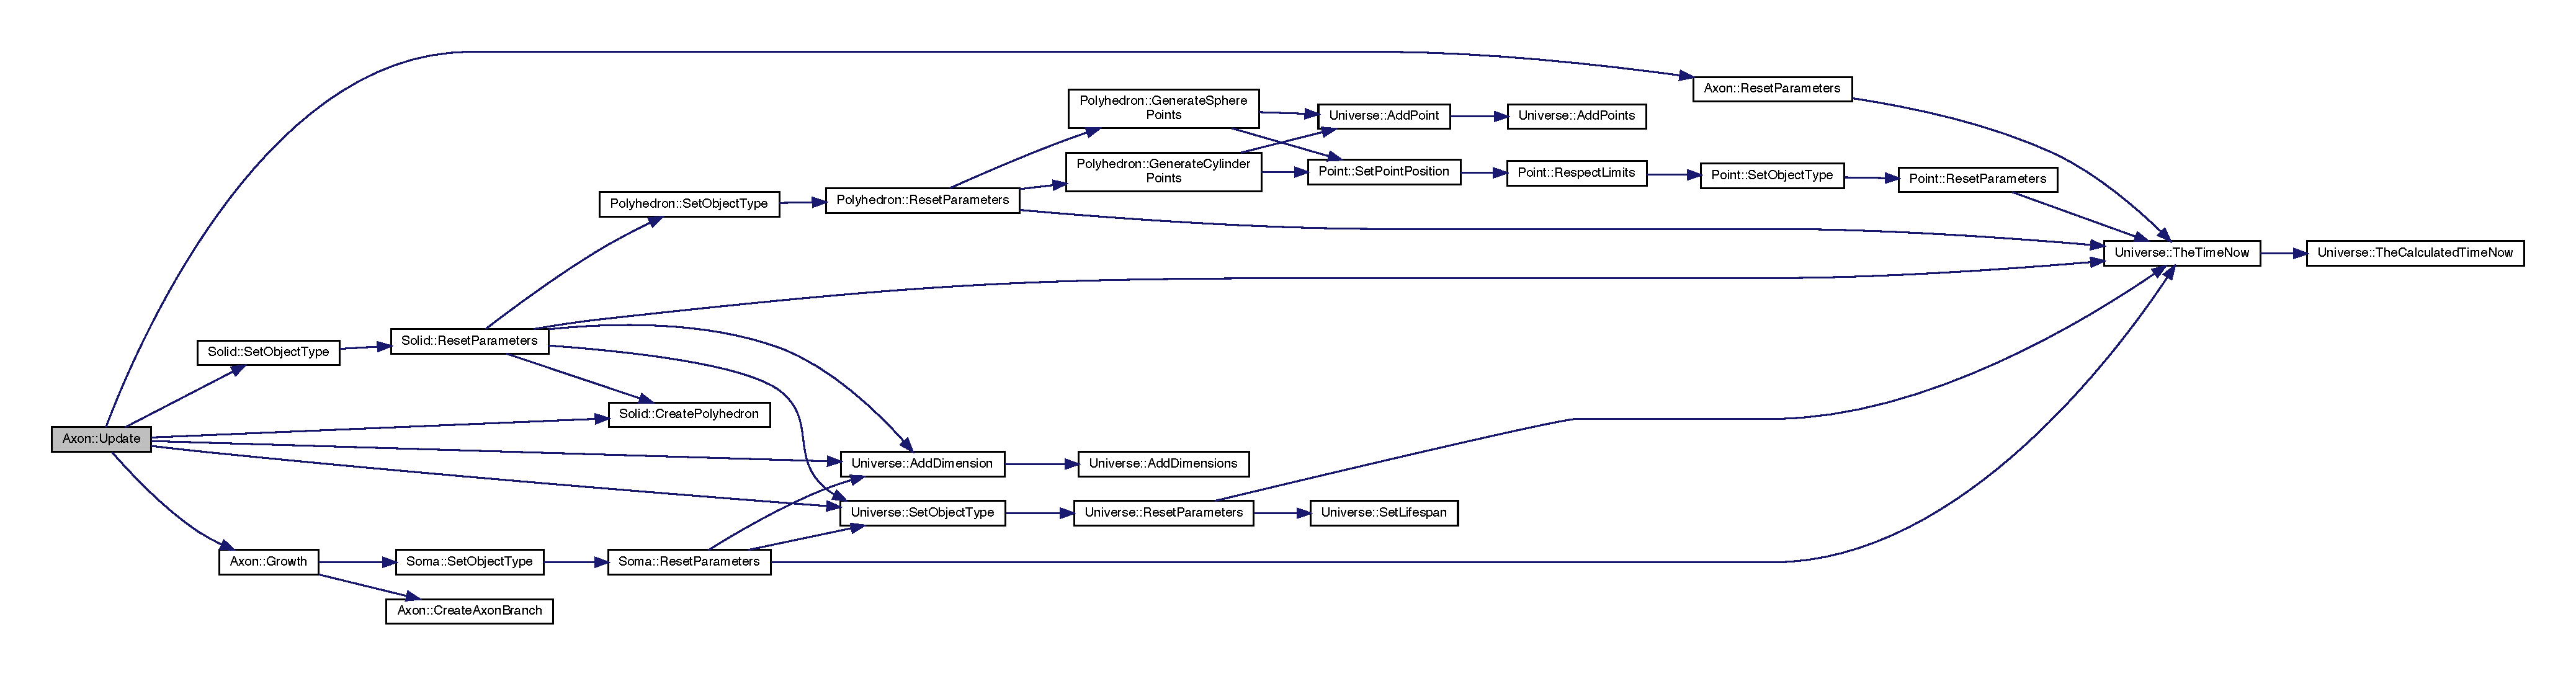
\includegraphics[width=350pt]{class_axon_a472ee760a1727072afaff0035d1eedd9_cgraph}
\end{center}
\end{figure}


\subsection{Member Data Documentation}
\mbox{\Hypertarget{class_axon_ab32c0e4335cc4da8fe1aace7c16a88bf}\label{class_axon_ab32c0e4335cc4da8fe1aace7c16a88bf}} 
\index{Axon@{Axon}!axonbranch\+\_\+list@{axonbranch\+\_\+list}}
\index{axonbranch\+\_\+list@{axonbranch\+\_\+list}!Axon@{Axon}}
\subsubsection{\texorpdfstring{axonbranch\+\_\+list}{axonbranch\_list}}
{\footnotesize\ttfamily std\+::vector$<$\mbox{\hyperlink{class_axon}{Axon}}$\ast$$>$ Axon\+::axonbranch\+\_\+list\hspace{0.3cm}{\ttfamily [protected]}}



Definition at line 77 of file axon.\+h.



The documentation for this class was generated from the following files\+:\begin{DoxyCompactItemize}
\item 
Brain\+Harmonics/\mbox{\hyperlink{axon_8h}{axon.\+h}}\item 
Brain\+Harmonics/\mbox{\hyperlink{axon_8cc}{axon.\+cc}}\end{DoxyCompactItemize}

\hypertarget{class_axon_bouton}{}\section{Axon\+Bouton Class Reference}
\label{class_axon_bouton}\index{Axon\+Bouton@{Axon\+Bouton}}


{\ttfamily \#include $<$axonbouton.\+h$>$}



Inheritance diagram for Axon\+Bouton\+:\nopagebreak
\begin{figure}[H]
\begin{center}
\leavevmode
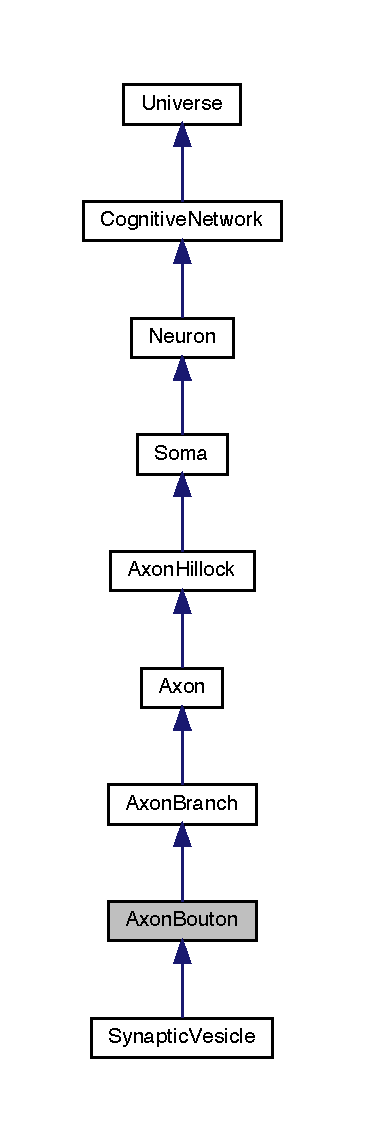
\includegraphics[width=175pt]{class_axon_bouton__inherit__graph}
\end{center}
\end{figure}


Collaboration diagram for Axon\+Bouton\+:\nopagebreak
\begin{figure}[H]
\begin{center}
\leavevmode
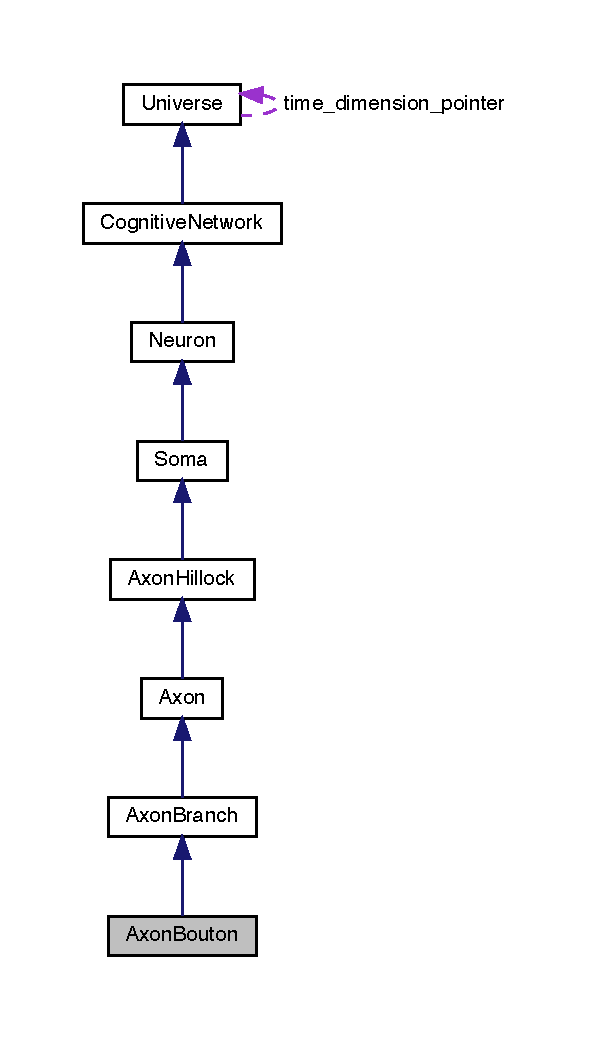
\includegraphics[width=283pt]{class_axon_bouton__coll__graph}
\end{center}
\end{figure}
\subsection*{Public Member Functions}
\begin{DoxyCompactItemize}
\item 
\mbox{\hyperlink{class_axon_bouton_acd6521d65ecb2b86abf2e3a8b322699e}{Axon\+Bouton}} ()
\item 
\mbox{\hyperlink{class_axon_bouton_a8a2da76b259a5ebab397fbd89d8b0632}{Axon\+Bouton}} (unsigned int object\+\_\+type)
\item 
\mbox{\hyperlink{class_axon_bouton_a93e33d72d90801d29d2b16ef94b59fab}{Axon\+Bouton}} (unsigned int object\+\_\+type, std\+::chrono\+::time\+\_\+point$<$ \mbox{\hyperlink{universe_8h_a0ef8d951d1ca5ab3cfaf7ab4c7a6fd80}{Clock}} $>$ event\+\_\+time)
\item 
\mbox{\hyperlink{class_axon_bouton_a6d671fc3b6bd8e617085c1bc7212400d}{Axon\+Bouton}} (unsigned int object\+\_\+type, std\+::chrono\+::time\+\_\+point$<$ \mbox{\hyperlink{universe_8h_a0ef8d951d1ca5ab3cfaf7ab4c7a6fd80}{Clock}} $>$ event\+\_\+time, \mbox{\hyperlink{class_axon_branch}{Axon\+Branch}} \&axonbranch\+\_\+connector)
\item 
virtual \mbox{\hyperlink{class_axon_bouton_ab6f93f680d19d4f07476d1d1b3de776a}{$\sim$\+Axon\+Bouton}} ()
\item 
unsigned int \mbox{\hyperlink{class_axon_bouton_a251fc23f754c077cf43ee68991b81624}{Get\+Counter}} (std\+::chrono\+::time\+\_\+point$<$ \mbox{\hyperlink{universe_8h_a0ef8d951d1ca5ab3cfaf7ab4c7a6fd80}{Clock}} $>$ event\+\_\+time)
\item 
double \mbox{\hyperlink{class_axon_bouton_a8dff077a40565f4e3a34388a6c38a603}{Get\+Energy}} (std\+::chrono\+::time\+\_\+point$<$ \mbox{\hyperlink{universe_8h_a0ef8d951d1ca5ab3cfaf7ab4c7a6fd80}{Clock}} $>$ event\+\_\+time)
\item 
\mbox{\hyperlink{glad_8h_a950fc91edb4504f62f1c577bf4727c29}{void}} \mbox{\hyperlink{class_axon_bouton_afe285478d414f2815afb98abe7b92898}{Set\+Counter}} (std\+::chrono\+::time\+\_\+point$<$ \mbox{\hyperlink{universe_8h_a0ef8d951d1ca5ab3cfaf7ab4c7a6fd80}{Clock}} $>$ event\+\_\+time, unsigned int \mbox{\hyperlink{glad_8h_a26942fd2ed566ef553eae82d2c109c8f}{val}})
\item 
\mbox{\hyperlink{glad_8h_a950fc91edb4504f62f1c577bf4727c29}{void}} \mbox{\hyperlink{class_axon_bouton_ab24fa467ab7221d0577e54734684a491}{Set\+Energy}} (std\+::chrono\+::time\+\_\+point$<$ \mbox{\hyperlink{universe_8h_a0ef8d951d1ca5ab3cfaf7ab4c7a6fd80}{Clock}} $>$ event\+\_\+time, double \mbox{\hyperlink{glad_8h_a26942fd2ed566ef553eae82d2c109c8f}{val}})
\item 
bool \mbox{\hyperlink{class_axon_bouton_a73d3721361c4e1ce6b110ffe1b4a7a88}{Reset\+Parameters}} (std\+::chrono\+::time\+\_\+point$<$ \mbox{\hyperlink{universe_8h_a0ef8d951d1ca5ab3cfaf7ab4c7a6fd80}{Clock}} $>$ event\+\_\+time)
\item 
\mbox{\hyperlink{class_axon_bouton}{Axon\+Bouton}} $\ast$ \mbox{\hyperlink{class_axon_bouton_a2aa0abe381f6e7c87c702189d01dfbf2}{Create\+Synaptic\+Vesicle}} (std\+::chrono\+::time\+\_\+point$<$ \mbox{\hyperlink{universe_8h_a0ef8d951d1ca5ab3cfaf7ab4c7a6fd80}{Clock}} $>$ event\+\_\+time)
\item 
std\+::vector$<$ \mbox{\hyperlink{class_axon_bouton}{Axon\+Bouton}} $\ast$ $>$ \mbox{\hyperlink{class_axon_bouton_a0cabe429536722f14ae800c8579168b7}{Create\+Synaptic\+Vesicles}} (std\+::chrono\+::time\+\_\+point$<$ \mbox{\hyperlink{universe_8h_a0ef8d951d1ca5ab3cfaf7ab4c7a6fd80}{Clock}} $>$ event\+\_\+time, int quantity)
\item 
\mbox{\hyperlink{class_axon_bouton}{Axon\+Bouton}} $\ast$ \mbox{\hyperlink{class_axon_bouton_a0e739b20447539f8db3655e83575fcf4}{Clone\+Synaptic\+Vesicle}} (std\+::chrono\+::time\+\_\+point$<$ \mbox{\hyperlink{universe_8h_a0ef8d951d1ca5ab3cfaf7ab4c7a6fd80}{Clock}} $>$ event\+\_\+time, \mbox{\hyperlink{class_axon_bouton}{Axon\+Bouton}} $\ast$clone\+\_\+object, double perfection\+\_\+membership)
\item 
std\+::vector$<$ \mbox{\hyperlink{class_axon_bouton}{Axon\+Bouton}} $\ast$ $>$ \mbox{\hyperlink{class_axon_bouton_a7bf1d8db3287dc5357d0095233f5c47f}{Clone\+Synaptic\+Vesicles}} (std\+::chrono\+::time\+\_\+point$<$ \mbox{\hyperlink{universe_8h_a0ef8d951d1ca5ab3cfaf7ab4c7a6fd80}{Clock}} $>$ event\+\_\+time, std\+::vector$<$ \mbox{\hyperlink{class_axon_bouton}{Axon\+Bouton}} $\ast$$>$ cloning\+\_\+list, double perfection\+\_\+membership)
\item 
\mbox{\hyperlink{class_axon_bouton}{Axon\+Bouton}} $\ast$ \mbox{\hyperlink{class_axon_bouton_a75592b4ccc589db756183f4aaa694ffe}{Destroy\+Synaptic\+Vesicle}} (std\+::chrono\+::time\+\_\+point$<$ \mbox{\hyperlink{universe_8h_a0ef8d951d1ca5ab3cfaf7ab4c7a6fd80}{Clock}} $>$ event\+\_\+time, \mbox{\hyperlink{class_axon_bouton}{Axon\+Bouton}} $\ast$destroy\+\_\+object)
\item 
std\+::vector$<$ \mbox{\hyperlink{class_axon_bouton}{Axon\+Bouton}} $\ast$ $>$ \mbox{\hyperlink{class_axon_bouton_a0fa1c238a29d9e2b84b4d9c556452150}{Destroy\+Synaptic\+Vesicles}} (std\+::chrono\+::time\+\_\+point$<$ \mbox{\hyperlink{universe_8h_a0ef8d951d1ca5ab3cfaf7ab4c7a6fd80}{Clock}} $>$ event\+\_\+time, std\+::vector$<$ \mbox{\hyperlink{class_axon_bouton}{Axon\+Bouton}} $\ast$$>$ destruction\+\_\+list)
\item 
\mbox{\hyperlink{class_axon_bouton}{Axon\+Bouton}} $\ast$ \mbox{\hyperlink{class_axon_bouton_a3009e5d49c699afa7f633b026b37ed77}{Add\+Synaptic\+Vesicle}} (std\+::chrono\+::time\+\_\+point$<$ \mbox{\hyperlink{universe_8h_a0ef8d951d1ca5ab3cfaf7ab4c7a6fd80}{Clock}} $>$ event\+\_\+time, \mbox{\hyperlink{class_axon_bouton}{Axon\+Bouton}} $\ast$add\+\_\+object)
\item 
std\+::vector$<$ \mbox{\hyperlink{class_axon_bouton}{Axon\+Bouton}} $\ast$ $>$ \mbox{\hyperlink{class_axon_bouton_a0e264da88f6ca5d77aa42f415cb4f3aa}{Add\+Synaptic\+Vesicles}} (std\+::chrono\+::time\+\_\+point$<$ \mbox{\hyperlink{universe_8h_a0ef8d951d1ca5ab3cfaf7ab4c7a6fd80}{Clock}} $>$ event\+\_\+time, std\+::vector$<$ \mbox{\hyperlink{class_axon_bouton}{Axon\+Bouton}} $\ast$$>$ add\+\_\+objects)
\item 
\mbox{\hyperlink{class_axon_bouton}{Axon\+Bouton}} $\ast$ \mbox{\hyperlink{class_axon_bouton_a1f0b13fa7ec408c9e0cfb22cea9bbe8c}{Remove\+Synaptic\+Vesicle}} (std\+::chrono\+::time\+\_\+point$<$ \mbox{\hyperlink{universe_8h_a0ef8d951d1ca5ab3cfaf7ab4c7a6fd80}{Clock}} $>$ event\+\_\+time)
\item 
std\+::vector$<$ \mbox{\hyperlink{class_axon_bouton}{Axon\+Bouton}} $\ast$ $>$ \mbox{\hyperlink{class_axon_bouton_ae4119170ef72beaed3c8a0eb1d80ef14}{Remove\+Synaptic\+Vesicles}} (std\+::chrono\+::time\+\_\+point$<$ \mbox{\hyperlink{universe_8h_a0ef8d951d1ca5ab3cfaf7ab4c7a6fd80}{Clock}} $>$ event\+\_\+time, int quantity)
\item 
\mbox{\hyperlink{class_axon_bouton}{Axon\+Bouton}} $\ast$ \mbox{\hyperlink{class_axon_bouton_a847ab3d3d214ddc85bdfd463c6d95d54}{Get\+Synaptic\+Vesicle}} (std\+::chrono\+::time\+\_\+point$<$ \mbox{\hyperlink{universe_8h_a0ef8d951d1ca5ab3cfaf7ab4c7a6fd80}{Clock}} $>$ event\+\_\+time, int selector)
\item 
std\+::vector$<$ \mbox{\hyperlink{class_axon_bouton}{Axon\+Bouton}} $\ast$ $>$ \mbox{\hyperlink{class_axon_bouton_af9a35ff7a6c32ac291021cccb3d40c9b}{Get\+Synaptic\+Vesicles}} (std\+::chrono\+::time\+\_\+point$<$ \mbox{\hyperlink{universe_8h_a0ef8d951d1ca5ab3cfaf7ab4c7a6fd80}{Clock}} $>$ event\+\_\+time)
\item 
int \mbox{\hyperlink{class_axon_bouton_a95fc006b2436e2c7784af2cc0bc9522e}{Growth\+Surface}} (std\+::chrono\+::time\+\_\+point$<$ \mbox{\hyperlink{universe_8h_a0ef8d951d1ca5ab3cfaf7ab4c7a6fd80}{Clock}} $>$ event\+\_\+time, double surf\+\_\+change)
\item 
int \mbox{\hyperlink{class_axon_bouton_a10ac4446e777376a3944c87b2bcf26b5}{Growth\+Volume}} (std\+::chrono\+::time\+\_\+point$<$ \mbox{\hyperlink{universe_8h_a0ef8d951d1ca5ab3cfaf7ab4c7a6fd80}{Clock}} $>$ event\+\_\+time, double vol\+\_\+change)
\item 
int \mbox{\hyperlink{class_axon_bouton_a26f89bac681b8f0894fe1ae249733917}{Update}} (std\+::chrono\+::time\+\_\+point$<$ \mbox{\hyperlink{universe_8h_a0ef8d951d1ca5ab3cfaf7ab4c7a6fd80}{Clock}} $>$ event\+\_\+time)
\end{DoxyCompactItemize}
\subsection*{Protected Attributes}
\begin{DoxyCompactItemize}
\item 
std\+::vector$<$ \mbox{\hyperlink{class_axon_bouton}{Axon\+Bouton}} $\ast$ $>$ \mbox{\hyperlink{class_axon_bouton_ad5b4e9b5fefb2ad9e6dfe5ad91be2dd7}{synapticvesicle\+\_\+list}}
\end{DoxyCompactItemize}
\subsection*{Additional Inherited Members}


\subsection{Detailed Description}


Definition at line 14 of file axonbouton.\+h.



\subsection{Constructor \& Destructor Documentation}
\mbox{\Hypertarget{class_axon_bouton_acd6521d65ecb2b86abf2e3a8b322699e}\label{class_axon_bouton_acd6521d65ecb2b86abf2e3a8b322699e}} 
\index{Axon\+Bouton@{Axon\+Bouton}!Axon\+Bouton@{Axon\+Bouton}}
\index{Axon\+Bouton@{Axon\+Bouton}!Axon\+Bouton@{Axon\+Bouton}}
\subsubsection{\texorpdfstring{Axon\+Bouton()}{AxonBouton()}\hspace{0.1cm}{\footnotesize\ttfamily [1/4]}}
{\footnotesize\ttfamily Axon\+Bouton\+::\+Axon\+Bouton (\begin{DoxyParamCaption}{ }\end{DoxyParamCaption})\hspace{0.3cm}{\ttfamily [inline]}}



Definition at line 17 of file axonbouton.\+h.

\mbox{\Hypertarget{class_axon_bouton_a8a2da76b259a5ebab397fbd89d8b0632}\label{class_axon_bouton_a8a2da76b259a5ebab397fbd89d8b0632}} 
\index{Axon\+Bouton@{Axon\+Bouton}!Axon\+Bouton@{Axon\+Bouton}}
\index{Axon\+Bouton@{Axon\+Bouton}!Axon\+Bouton@{Axon\+Bouton}}
\subsubsection{\texorpdfstring{Axon\+Bouton()}{AxonBouton()}\hspace{0.1cm}{\footnotesize\ttfamily [2/4]}}
{\footnotesize\ttfamily Axon\+Bouton\+::\+Axon\+Bouton (\begin{DoxyParamCaption}\item[{unsigned int}]{object\+\_\+type }\end{DoxyParamCaption})\hspace{0.3cm}{\ttfamily [inline]}}



Definition at line 19 of file axonbouton.\+h.

\mbox{\Hypertarget{class_axon_bouton_a93e33d72d90801d29d2b16ef94b59fab}\label{class_axon_bouton_a93e33d72d90801d29d2b16ef94b59fab}} 
\index{Axon\+Bouton@{Axon\+Bouton}!Axon\+Bouton@{Axon\+Bouton}}
\index{Axon\+Bouton@{Axon\+Bouton}!Axon\+Bouton@{Axon\+Bouton}}
\subsubsection{\texorpdfstring{Axon\+Bouton()}{AxonBouton()}\hspace{0.1cm}{\footnotesize\ttfamily [3/4]}}
{\footnotesize\ttfamily Axon\+Bouton\+::\+Axon\+Bouton (\begin{DoxyParamCaption}\item[{unsigned int}]{object\+\_\+type,  }\item[{std\+::chrono\+::time\+\_\+point$<$ \mbox{\hyperlink{universe_8h_a0ef8d951d1ca5ab3cfaf7ab4c7a6fd80}{Clock}} $>$}]{event\+\_\+time }\end{DoxyParamCaption})\hspace{0.3cm}{\ttfamily [inline]}}



Definition at line 21 of file axonbouton.\+h.

\mbox{\Hypertarget{class_axon_bouton_a6d671fc3b6bd8e617085c1bc7212400d}\label{class_axon_bouton_a6d671fc3b6bd8e617085c1bc7212400d}} 
\index{Axon\+Bouton@{Axon\+Bouton}!Axon\+Bouton@{Axon\+Bouton}}
\index{Axon\+Bouton@{Axon\+Bouton}!Axon\+Bouton@{Axon\+Bouton}}
\subsubsection{\texorpdfstring{Axon\+Bouton()}{AxonBouton()}\hspace{0.1cm}{\footnotesize\ttfamily [4/4]}}
{\footnotesize\ttfamily Axon\+Bouton\+::\+Axon\+Bouton (\begin{DoxyParamCaption}\item[{unsigned int}]{object\+\_\+type,  }\item[{std\+::chrono\+::time\+\_\+point$<$ \mbox{\hyperlink{universe_8h_a0ef8d951d1ca5ab3cfaf7ab4c7a6fd80}{Clock}} $>$}]{event\+\_\+time,  }\item[{\mbox{\hyperlink{class_axon_branch}{Axon\+Branch}} \&}]{axonbranch\+\_\+connector }\end{DoxyParamCaption})\hspace{0.3cm}{\ttfamily [inline]}}



Definition at line 23 of file axonbouton.\+h.

Here is the call graph for this function\+:\nopagebreak
\begin{figure}[H]
\begin{center}
\leavevmode
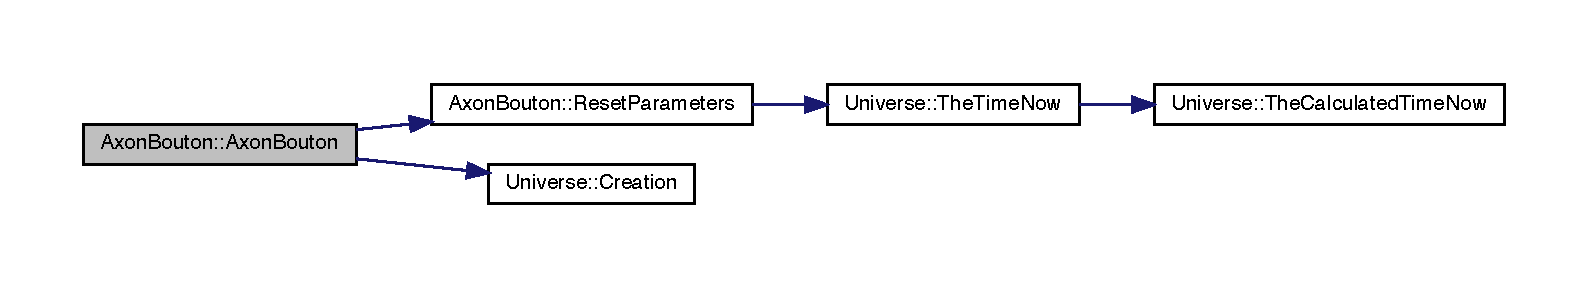
\includegraphics[width=350pt]{class_axon_bouton_a6d671fc3b6bd8e617085c1bc7212400d_cgraph}
\end{center}
\end{figure}
\mbox{\Hypertarget{class_axon_bouton_ab6f93f680d19d4f07476d1d1b3de776a}\label{class_axon_bouton_ab6f93f680d19d4f07476d1d1b3de776a}} 
\index{Axon\+Bouton@{Axon\+Bouton}!````~Axon\+Bouton@{$\sim$\+Axon\+Bouton}}
\index{````~Axon\+Bouton@{$\sim$\+Axon\+Bouton}!Axon\+Bouton@{Axon\+Bouton}}
\subsubsection{\texorpdfstring{$\sim$\+Axon\+Bouton()}{~AxonBouton()}}
{\footnotesize\ttfamily virtual Axon\+Bouton\+::$\sim$\+Axon\+Bouton (\begin{DoxyParamCaption}{ }\end{DoxyParamCaption})\hspace{0.3cm}{\ttfamily [inline]}, {\ttfamily [virtual]}}

Default destructor 

Definition at line 36 of file axonbouton.\+h.



\subsection{Member Function Documentation}
\mbox{\Hypertarget{class_axon_bouton_a3009e5d49c699afa7f633b026b37ed77}\label{class_axon_bouton_a3009e5d49c699afa7f633b026b37ed77}} 
\index{Axon\+Bouton@{Axon\+Bouton}!Add\+Synaptic\+Vesicle@{Add\+Synaptic\+Vesicle}}
\index{Add\+Synaptic\+Vesicle@{Add\+Synaptic\+Vesicle}!Axon\+Bouton@{Axon\+Bouton}}
\subsubsection{\texorpdfstring{Add\+Synaptic\+Vesicle()}{AddSynapticVesicle()}}
{\footnotesize\ttfamily \mbox{\hyperlink{class_axon_bouton}{Axon\+Bouton}} $\ast$ Axon\+Bouton\+::\+Add\+Synaptic\+Vesicle (\begin{DoxyParamCaption}\item[{std\+::chrono\+::time\+\_\+point$<$ \mbox{\hyperlink{universe_8h_a0ef8d951d1ca5ab3cfaf7ab4c7a6fd80}{Clock}} $>$}]{event\+\_\+time,  }\item[{\mbox{\hyperlink{class_axon_bouton}{Axon\+Bouton}} $\ast$}]{add\+\_\+object }\end{DoxyParamCaption})}



Definition at line 115 of file axonbouton.\+cc.

Here is the caller graph for this function\+:\nopagebreak
\begin{figure}[H]
\begin{center}
\leavevmode
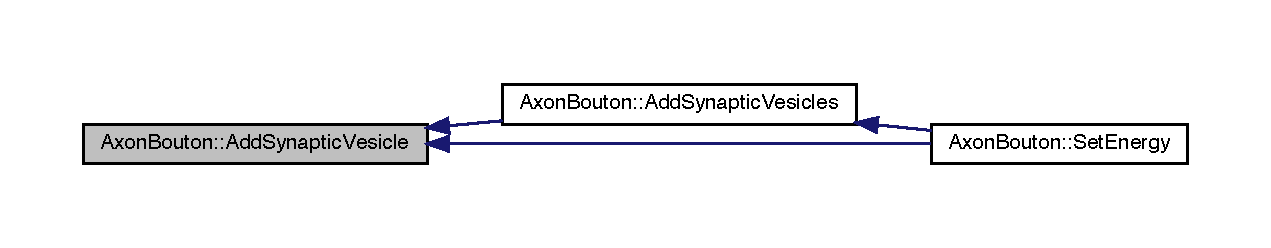
\includegraphics[width=350pt]{class_axon_bouton_a3009e5d49c699afa7f633b026b37ed77_icgraph}
\end{center}
\end{figure}
\mbox{\Hypertarget{class_axon_bouton_a0e264da88f6ca5d77aa42f415cb4f3aa}\label{class_axon_bouton_a0e264da88f6ca5d77aa42f415cb4f3aa}} 
\index{Axon\+Bouton@{Axon\+Bouton}!Add\+Synaptic\+Vesicles@{Add\+Synaptic\+Vesicles}}
\index{Add\+Synaptic\+Vesicles@{Add\+Synaptic\+Vesicles}!Axon\+Bouton@{Axon\+Bouton}}
\subsubsection{\texorpdfstring{Add\+Synaptic\+Vesicles()}{AddSynapticVesicles()}}
{\footnotesize\ttfamily std\+::vector$<$ \mbox{\hyperlink{class_axon_bouton}{Axon\+Bouton}} $\ast$ $>$ Axon\+Bouton\+::\+Add\+Synaptic\+Vesicles (\begin{DoxyParamCaption}\item[{std\+::chrono\+::time\+\_\+point$<$ \mbox{\hyperlink{universe_8h_a0ef8d951d1ca5ab3cfaf7ab4c7a6fd80}{Clock}} $>$}]{event\+\_\+time,  }\item[{std\+::vector$<$ \mbox{\hyperlink{class_axon_bouton}{Axon\+Bouton}} $\ast$$>$}]{add\+\_\+objects }\end{DoxyParamCaption})}



Definition at line 126 of file axonbouton.\+cc.

Here is the call graph for this function\+:\nopagebreak
\begin{figure}[H]
\begin{center}
\leavevmode
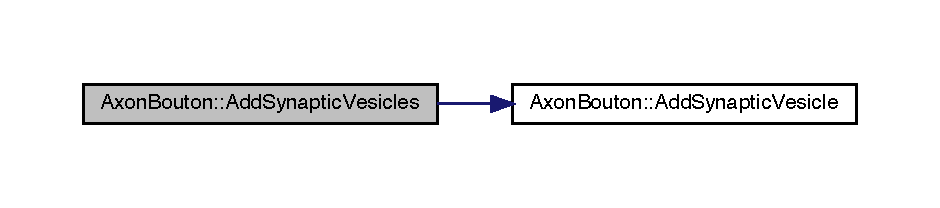
\includegraphics[width=350pt]{class_axon_bouton_a0e264da88f6ca5d77aa42f415cb4f3aa_cgraph}
\end{center}
\end{figure}
\mbox{\Hypertarget{class_axon_bouton_a0e739b20447539f8db3655e83575fcf4}\label{class_axon_bouton_a0e739b20447539f8db3655e83575fcf4}} 
\index{Axon\+Bouton@{Axon\+Bouton}!Clone\+Synaptic\+Vesicle@{Clone\+Synaptic\+Vesicle}}
\index{Clone\+Synaptic\+Vesicle@{Clone\+Synaptic\+Vesicle}!Axon\+Bouton@{Axon\+Bouton}}
\subsubsection{\texorpdfstring{Clone\+Synaptic\+Vesicle()}{CloneSynapticVesicle()}}
{\footnotesize\ttfamily \mbox{\hyperlink{class_axon_bouton}{Axon\+Bouton}} $\ast$ Axon\+Bouton\+::\+Clone\+Synaptic\+Vesicle (\begin{DoxyParamCaption}\item[{std\+::chrono\+::time\+\_\+point$<$ \mbox{\hyperlink{universe_8h_a0ef8d951d1ca5ab3cfaf7ab4c7a6fd80}{Clock}} $>$}]{event\+\_\+time,  }\item[{\mbox{\hyperlink{class_axon_bouton}{Axon\+Bouton}} $\ast$}]{clone\+\_\+object,  }\item[{double}]{perfection\+\_\+membership }\end{DoxyParamCaption})}



Definition at line 100 of file axonbouton.\+cc.

\mbox{\Hypertarget{class_axon_bouton_a7bf1d8db3287dc5357d0095233f5c47f}\label{class_axon_bouton_a7bf1d8db3287dc5357d0095233f5c47f}} 
\index{Axon\+Bouton@{Axon\+Bouton}!Clone\+Synaptic\+Vesicles@{Clone\+Synaptic\+Vesicles}}
\index{Clone\+Synaptic\+Vesicles@{Clone\+Synaptic\+Vesicles}!Axon\+Bouton@{Axon\+Bouton}}
\subsubsection{\texorpdfstring{Clone\+Synaptic\+Vesicles()}{CloneSynapticVesicles()}}
{\footnotesize\ttfamily std\+::vector$<$ \mbox{\hyperlink{class_axon_bouton}{Axon\+Bouton}} $\ast$ $>$ Axon\+Bouton\+::\+Clone\+Synaptic\+Vesicles (\begin{DoxyParamCaption}\item[{std\+::chrono\+::time\+\_\+point$<$ \mbox{\hyperlink{universe_8h_a0ef8d951d1ca5ab3cfaf7ab4c7a6fd80}{Clock}} $>$}]{event\+\_\+time,  }\item[{std\+::vector$<$ \mbox{\hyperlink{class_axon_bouton}{Axon\+Bouton}} $\ast$$>$}]{cloning\+\_\+list,  }\item[{double}]{perfection\+\_\+membership }\end{DoxyParamCaption})}



Definition at line 95 of file axonbouton.\+cc.

\mbox{\Hypertarget{class_axon_bouton_a2aa0abe381f6e7c87c702189d01dfbf2}\label{class_axon_bouton_a2aa0abe381f6e7c87c702189d01dfbf2}} 
\index{Axon\+Bouton@{Axon\+Bouton}!Create\+Synaptic\+Vesicle@{Create\+Synaptic\+Vesicle}}
\index{Create\+Synaptic\+Vesicle@{Create\+Synaptic\+Vesicle}!Axon\+Bouton@{Axon\+Bouton}}
\subsubsection{\texorpdfstring{Create\+Synaptic\+Vesicle()}{CreateSynapticVesicle()}}
{\footnotesize\ttfamily \mbox{\hyperlink{class_axon_bouton}{Axon\+Bouton}} $\ast$ Axon\+Bouton\+::\+Create\+Synaptic\+Vesicle (\begin{DoxyParamCaption}\item[{std\+::chrono\+::time\+\_\+point$<$ \mbox{\hyperlink{universe_8h_a0ef8d951d1ca5ab3cfaf7ab4c7a6fd80}{Clock}} $>$}]{event\+\_\+time }\end{DoxyParamCaption})}



Definition at line 62 of file axonbouton.\+cc.

Here is the caller graph for this function\+:\nopagebreak
\begin{figure}[H]
\begin{center}
\leavevmode
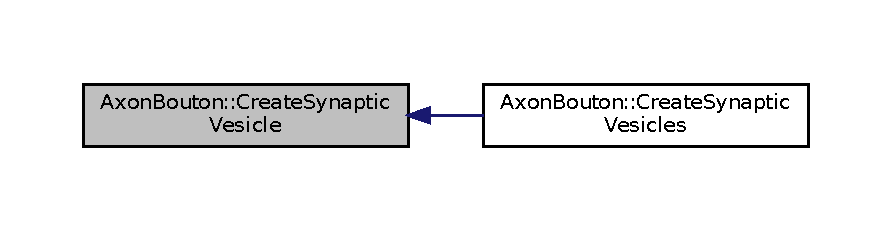
\includegraphics[width=350pt]{class_axon_bouton_a2aa0abe381f6e7c87c702189d01dfbf2_icgraph}
\end{center}
\end{figure}
\mbox{\Hypertarget{class_axon_bouton_a0cabe429536722f14ae800c8579168b7}\label{class_axon_bouton_a0cabe429536722f14ae800c8579168b7}} 
\index{Axon\+Bouton@{Axon\+Bouton}!Create\+Synaptic\+Vesicles@{Create\+Synaptic\+Vesicles}}
\index{Create\+Synaptic\+Vesicles@{Create\+Synaptic\+Vesicles}!Axon\+Bouton@{Axon\+Bouton}}
\subsubsection{\texorpdfstring{Create\+Synaptic\+Vesicles()}{CreateSynapticVesicles()}}
{\footnotesize\ttfamily std\+::vector$<$ \mbox{\hyperlink{class_axon_bouton}{Axon\+Bouton}} $\ast$ $>$ Axon\+Bouton\+::\+Create\+Synaptic\+Vesicles (\begin{DoxyParamCaption}\item[{std\+::chrono\+::time\+\_\+point$<$ \mbox{\hyperlink{universe_8h_a0ef8d951d1ca5ab3cfaf7ab4c7a6fd80}{Clock}} $>$}]{event\+\_\+time,  }\item[{int}]{quantity }\end{DoxyParamCaption})}



Definition at line 73 of file axonbouton.\+cc.

Here is the call graph for this function\+:\nopagebreak
\begin{figure}[H]
\begin{center}
\leavevmode
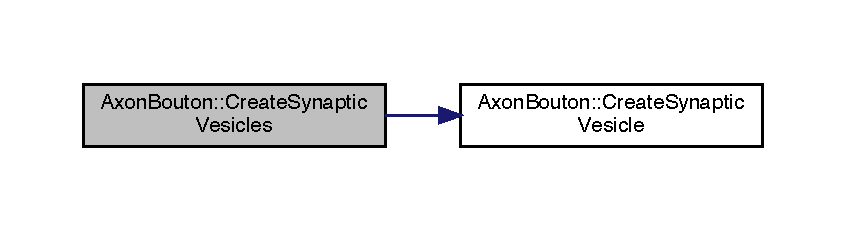
\includegraphics[width=350pt]{class_axon_bouton_a0cabe429536722f14ae800c8579168b7_cgraph}
\end{center}
\end{figure}
\mbox{\Hypertarget{class_axon_bouton_a75592b4ccc589db756183f4aaa694ffe}\label{class_axon_bouton_a75592b4ccc589db756183f4aaa694ffe}} 
\index{Axon\+Bouton@{Axon\+Bouton}!Destroy\+Synaptic\+Vesicle@{Destroy\+Synaptic\+Vesicle}}
\index{Destroy\+Synaptic\+Vesicle@{Destroy\+Synaptic\+Vesicle}!Axon\+Bouton@{Axon\+Bouton}}
\subsubsection{\texorpdfstring{Destroy\+Synaptic\+Vesicle()}{DestroySynapticVesicle()}}
{\footnotesize\ttfamily \mbox{\hyperlink{class_axon_bouton}{Axon\+Bouton}} $\ast$ Axon\+Bouton\+::\+Destroy\+Synaptic\+Vesicle (\begin{DoxyParamCaption}\item[{std\+::chrono\+::time\+\_\+point$<$ \mbox{\hyperlink{universe_8h_a0ef8d951d1ca5ab3cfaf7ab4c7a6fd80}{Clock}} $>$}]{event\+\_\+time,  }\item[{\mbox{\hyperlink{class_axon_bouton}{Axon\+Bouton}} $\ast$}]{destroy\+\_\+object }\end{DoxyParamCaption})}



Definition at line 110 of file axonbouton.\+cc.

\mbox{\Hypertarget{class_axon_bouton_a0fa1c238a29d9e2b84b4d9c556452150}\label{class_axon_bouton_a0fa1c238a29d9e2b84b4d9c556452150}} 
\index{Axon\+Bouton@{Axon\+Bouton}!Destroy\+Synaptic\+Vesicles@{Destroy\+Synaptic\+Vesicles}}
\index{Destroy\+Synaptic\+Vesicles@{Destroy\+Synaptic\+Vesicles}!Axon\+Bouton@{Axon\+Bouton}}
\subsubsection{\texorpdfstring{Destroy\+Synaptic\+Vesicles()}{DestroySynapticVesicles()}}
{\footnotesize\ttfamily std\+::vector$<$ \mbox{\hyperlink{class_axon_bouton}{Axon\+Bouton}} $\ast$ $>$ Axon\+Bouton\+::\+Destroy\+Synaptic\+Vesicles (\begin{DoxyParamCaption}\item[{std\+::chrono\+::time\+\_\+point$<$ \mbox{\hyperlink{universe_8h_a0ef8d951d1ca5ab3cfaf7ab4c7a6fd80}{Clock}} $>$}]{event\+\_\+time,  }\item[{std\+::vector$<$ \mbox{\hyperlink{class_axon_bouton}{Axon\+Bouton}} $\ast$$>$}]{destruction\+\_\+list }\end{DoxyParamCaption})}



Definition at line 105 of file axonbouton.\+cc.

\mbox{\Hypertarget{class_axon_bouton_a251fc23f754c077cf43ee68991b81624}\label{class_axon_bouton_a251fc23f754c077cf43ee68991b81624}} 
\index{Axon\+Bouton@{Axon\+Bouton}!Get\+Counter@{Get\+Counter}}
\index{Get\+Counter@{Get\+Counter}!Axon\+Bouton@{Axon\+Bouton}}
\subsubsection{\texorpdfstring{Get\+Counter()}{GetCounter()}}
{\footnotesize\ttfamily unsigned int Axon\+Bouton\+::\+Get\+Counter (\begin{DoxyParamCaption}\item[{std\+::chrono\+::time\+\_\+point$<$ \mbox{\hyperlink{universe_8h_a0ef8d951d1ca5ab3cfaf7ab4c7a6fd80}{Clock}} $>$}]{event\+\_\+time }\end{DoxyParamCaption})\hspace{0.3cm}{\ttfamily [inline]}}



Definition at line 37 of file axonbouton.\+h.

\mbox{\Hypertarget{class_axon_bouton_a8dff077a40565f4e3a34388a6c38a603}\label{class_axon_bouton_a8dff077a40565f4e3a34388a6c38a603}} 
\index{Axon\+Bouton@{Axon\+Bouton}!Get\+Energy@{Get\+Energy}}
\index{Get\+Energy@{Get\+Energy}!Axon\+Bouton@{Axon\+Bouton}}
\subsubsection{\texorpdfstring{Get\+Energy()}{GetEnergy()}}
{\footnotesize\ttfamily double Axon\+Bouton\+::\+Get\+Energy (\begin{DoxyParamCaption}\item[{std\+::chrono\+::time\+\_\+point$<$ \mbox{\hyperlink{universe_8h_a0ef8d951d1ca5ab3cfaf7ab4c7a6fd80}{Clock}} $>$}]{event\+\_\+time }\end{DoxyParamCaption})\hspace{0.3cm}{\ttfamily [inline]}}



Definition at line 38 of file axonbouton.\+h.

\mbox{\Hypertarget{class_axon_bouton_a847ab3d3d214ddc85bdfd463c6d95d54}\label{class_axon_bouton_a847ab3d3d214ddc85bdfd463c6d95d54}} 
\index{Axon\+Bouton@{Axon\+Bouton}!Get\+Synaptic\+Vesicle@{Get\+Synaptic\+Vesicle}}
\index{Get\+Synaptic\+Vesicle@{Get\+Synaptic\+Vesicle}!Axon\+Bouton@{Axon\+Bouton}}
\subsubsection{\texorpdfstring{Get\+Synaptic\+Vesicle()}{GetSynapticVesicle()}}
{\footnotesize\ttfamily \mbox{\hyperlink{class_axon_bouton}{Axon\+Bouton}} $\ast$ Axon\+Bouton\+::\+Get\+Synaptic\+Vesicle (\begin{DoxyParamCaption}\item[{std\+::chrono\+::time\+\_\+point$<$ \mbox{\hyperlink{universe_8h_a0ef8d951d1ca5ab3cfaf7ab4c7a6fd80}{Clock}} $>$}]{event\+\_\+time,  }\item[{int}]{selector }\end{DoxyParamCaption})}



Definition at line 159 of file axonbouton.\+cc.

\mbox{\Hypertarget{class_axon_bouton_af9a35ff7a6c32ac291021cccb3d40c9b}\label{class_axon_bouton_af9a35ff7a6c32ac291021cccb3d40c9b}} 
\index{Axon\+Bouton@{Axon\+Bouton}!Get\+Synaptic\+Vesicles@{Get\+Synaptic\+Vesicles}}
\index{Get\+Synaptic\+Vesicles@{Get\+Synaptic\+Vesicles}!Axon\+Bouton@{Axon\+Bouton}}
\subsubsection{\texorpdfstring{Get\+Synaptic\+Vesicles()}{GetSynapticVesicles()}}
{\footnotesize\ttfamily std\+::vector$<$ \mbox{\hyperlink{class_axon_bouton}{Axon\+Bouton}} $\ast$ $>$ Axon\+Bouton\+::\+Get\+Synaptic\+Vesicles (\begin{DoxyParamCaption}\item[{std\+::chrono\+::time\+\_\+point$<$ \mbox{\hyperlink{universe_8h_a0ef8d951d1ca5ab3cfaf7ab4c7a6fd80}{Clock}} $>$}]{event\+\_\+time }\end{DoxyParamCaption})}



Definition at line 164 of file axonbouton.\+cc.

\mbox{\Hypertarget{class_axon_bouton_a95fc006b2436e2c7784af2cc0bc9522e}\label{class_axon_bouton_a95fc006b2436e2c7784af2cc0bc9522e}} 
\index{Axon\+Bouton@{Axon\+Bouton}!Growth\+Surface@{Growth\+Surface}}
\index{Growth\+Surface@{Growth\+Surface}!Axon\+Bouton@{Axon\+Bouton}}
\subsubsection{\texorpdfstring{Growth\+Surface()}{GrowthSurface()}}
{\footnotesize\ttfamily int Axon\+Bouton\+::\+Growth\+Surface (\begin{DoxyParamCaption}\item[{std\+::chrono\+::time\+\_\+point$<$ \mbox{\hyperlink{universe_8h_a0ef8d951d1ca5ab3cfaf7ab4c7a6fd80}{Clock}} $>$}]{event\+\_\+time,  }\item[{double}]{surf\+\_\+change }\end{DoxyParamCaption})}



Definition at line 169 of file axonbouton.\+cc.

Here is the caller graph for this function\+:\nopagebreak
\begin{figure}[H]
\begin{center}
\leavevmode
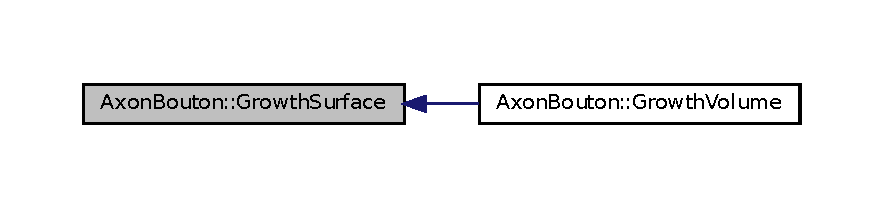
\includegraphics[width=350pt]{class_axon_bouton_a95fc006b2436e2c7784af2cc0bc9522e_icgraph}
\end{center}
\end{figure}
\mbox{\Hypertarget{class_axon_bouton_a10ac4446e777376a3944c87b2bcf26b5}\label{class_axon_bouton_a10ac4446e777376a3944c87b2bcf26b5}} 
\index{Axon\+Bouton@{Axon\+Bouton}!Growth\+Volume@{Growth\+Volume}}
\index{Growth\+Volume@{Growth\+Volume}!Axon\+Bouton@{Axon\+Bouton}}
\subsubsection{\texorpdfstring{Growth\+Volume()}{GrowthVolume()}}
{\footnotesize\ttfamily int Axon\+Bouton\+::\+Growth\+Volume (\begin{DoxyParamCaption}\item[{std\+::chrono\+::time\+\_\+point$<$ \mbox{\hyperlink{universe_8h_a0ef8d951d1ca5ab3cfaf7ab4c7a6fd80}{Clock}} $>$}]{event\+\_\+time,  }\item[{double}]{vol\+\_\+change }\end{DoxyParamCaption})}



Definition at line 176 of file axonbouton.\+cc.

Here is the call graph for this function\+:\nopagebreak
\begin{figure}[H]
\begin{center}
\leavevmode
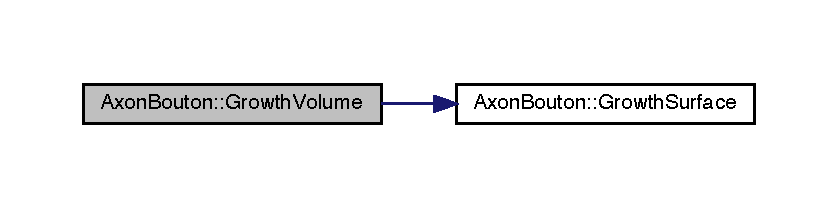
\includegraphics[width=350pt]{class_axon_bouton_a10ac4446e777376a3944c87b2bcf26b5_cgraph}
\end{center}
\end{figure}
\mbox{\Hypertarget{class_axon_bouton_a1f0b13fa7ec408c9e0cfb22cea9bbe8c}\label{class_axon_bouton_a1f0b13fa7ec408c9e0cfb22cea9bbe8c}} 
\index{Axon\+Bouton@{Axon\+Bouton}!Remove\+Synaptic\+Vesicle@{Remove\+Synaptic\+Vesicle}}
\index{Remove\+Synaptic\+Vesicle@{Remove\+Synaptic\+Vesicle}!Axon\+Bouton@{Axon\+Bouton}}
\subsubsection{\texorpdfstring{Remove\+Synaptic\+Vesicle()}{RemoveSynapticVesicle()}}
{\footnotesize\ttfamily \mbox{\hyperlink{class_axon_bouton}{Axon\+Bouton}} $\ast$ Axon\+Bouton\+::\+Remove\+Synaptic\+Vesicle (\begin{DoxyParamCaption}\item[{std\+::chrono\+::time\+\_\+point$<$ \mbox{\hyperlink{universe_8h_a0ef8d951d1ca5ab3cfaf7ab4c7a6fd80}{Clock}} $>$}]{event\+\_\+time }\end{DoxyParamCaption})}



Definition at line 148 of file axonbouton.\+cc.

\mbox{\Hypertarget{class_axon_bouton_ae4119170ef72beaed3c8a0eb1d80ef14}\label{class_axon_bouton_ae4119170ef72beaed3c8a0eb1d80ef14}} 
\index{Axon\+Bouton@{Axon\+Bouton}!Remove\+Synaptic\+Vesicles@{Remove\+Synaptic\+Vesicles}}
\index{Remove\+Synaptic\+Vesicles@{Remove\+Synaptic\+Vesicles}!Axon\+Bouton@{Axon\+Bouton}}
\subsubsection{\texorpdfstring{Remove\+Synaptic\+Vesicles()}{RemoveSynapticVesicles()}}
{\footnotesize\ttfamily std\+::vector$<$ \mbox{\hyperlink{class_axon_bouton}{Axon\+Bouton}} $\ast$ $>$ Axon\+Bouton\+::\+Remove\+Synaptic\+Vesicles (\begin{DoxyParamCaption}\item[{std\+::chrono\+::time\+\_\+point$<$ \mbox{\hyperlink{universe_8h_a0ef8d951d1ca5ab3cfaf7ab4c7a6fd80}{Clock}} $>$}]{event\+\_\+time,  }\item[{int}]{quantity }\end{DoxyParamCaption})}



Definition at line 154 of file axonbouton.\+cc.

\mbox{\Hypertarget{class_axon_bouton_a73d3721361c4e1ce6b110ffe1b4a7a88}\label{class_axon_bouton_a73d3721361c4e1ce6b110ffe1b4a7a88}} 
\index{Axon\+Bouton@{Axon\+Bouton}!Reset\+Parameters@{Reset\+Parameters}}
\index{Reset\+Parameters@{Reset\+Parameters}!Axon\+Bouton@{Axon\+Bouton}}
\subsubsection{\texorpdfstring{Reset\+Parameters()}{ResetParameters()}}
{\footnotesize\ttfamily bool Axon\+Bouton\+::\+Reset\+Parameters (\begin{DoxyParamCaption}\item[{std\+::chrono\+::time\+\_\+point$<$ \mbox{\hyperlink{universe_8h_a0ef8d951d1ca5ab3cfaf7ab4c7a6fd80}{Clock}} $>$}]{event\+\_\+time }\end{DoxyParamCaption})}



Definition at line 21 of file axonbouton.\+cc.

Here is the call graph for this function\+:\nopagebreak
\begin{figure}[H]
\begin{center}
\leavevmode
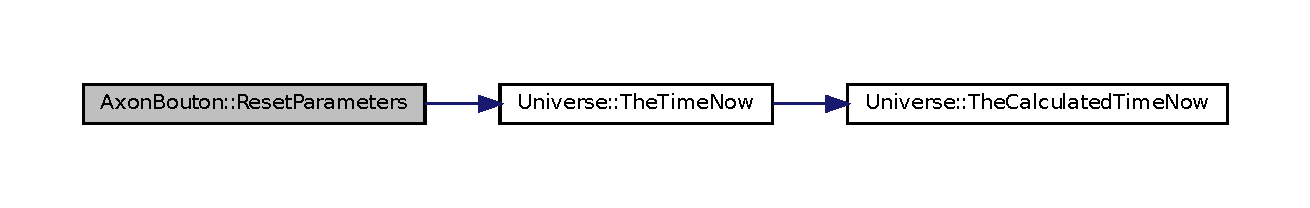
\includegraphics[width=350pt]{class_axon_bouton_a73d3721361c4e1ce6b110ffe1b4a7a88_cgraph}
\end{center}
\end{figure}
Here is the caller graph for this function\+:\nopagebreak
\begin{figure}[H]
\begin{center}
\leavevmode
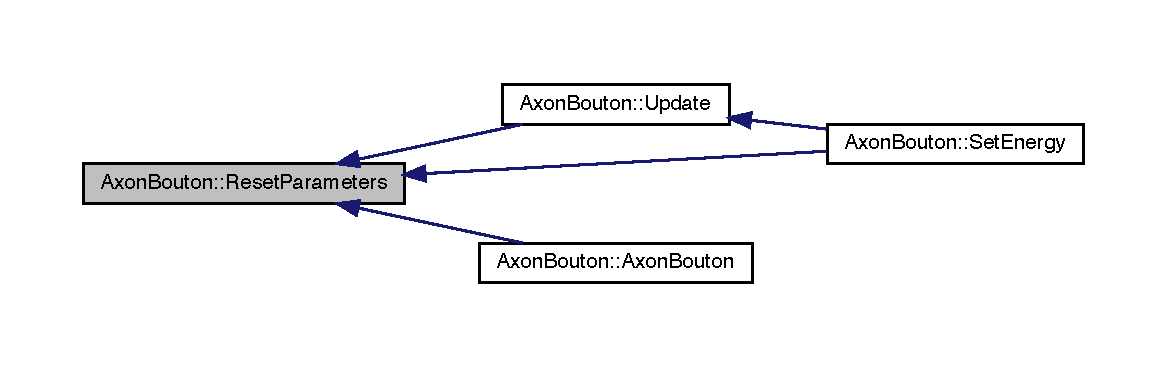
\includegraphics[width=350pt]{class_axon_bouton_a73d3721361c4e1ce6b110ffe1b4a7a88_icgraph}
\end{center}
\end{figure}
\mbox{\Hypertarget{class_axon_bouton_afe285478d414f2815afb98abe7b92898}\label{class_axon_bouton_afe285478d414f2815afb98abe7b92898}} 
\index{Axon\+Bouton@{Axon\+Bouton}!Set\+Counter@{Set\+Counter}}
\index{Set\+Counter@{Set\+Counter}!Axon\+Bouton@{Axon\+Bouton}}
\subsubsection{\texorpdfstring{Set\+Counter()}{SetCounter()}}
{\footnotesize\ttfamily \mbox{\hyperlink{glad_8h_a950fc91edb4504f62f1c577bf4727c29}{void}} Axon\+Bouton\+::\+Set\+Counter (\begin{DoxyParamCaption}\item[{std\+::chrono\+::time\+\_\+point$<$ \mbox{\hyperlink{universe_8h_a0ef8d951d1ca5ab3cfaf7ab4c7a6fd80}{Clock}} $>$}]{event\+\_\+time,  }\item[{unsigned int}]{val }\end{DoxyParamCaption})\hspace{0.3cm}{\ttfamily [inline]}, {\ttfamily [virtual]}}



Reimplemented from \mbox{\hyperlink{class_axon_a3493cb97bde26bd66facc6084cd5f219}{Axon}}.



Reimplemented in \mbox{\hyperlink{class_synaptic_vesicle_a7fd7cfce5eccb904206d968866f85220}{Synaptic\+Vesicle}}.



Definition at line 40 of file axonbouton.\+h.

\mbox{\Hypertarget{class_axon_bouton_ab24fa467ab7221d0577e54734684a491}\label{class_axon_bouton_ab24fa467ab7221d0577e54734684a491}} 
\index{Axon\+Bouton@{Axon\+Bouton}!Set\+Energy@{Set\+Energy}}
\index{Set\+Energy@{Set\+Energy}!Axon\+Bouton@{Axon\+Bouton}}
\subsubsection{\texorpdfstring{Set\+Energy()}{SetEnergy()}}
{\footnotesize\ttfamily \mbox{\hyperlink{glad_8h_a950fc91edb4504f62f1c577bf4727c29}{void}} Axon\+Bouton\+::\+Set\+Energy (\begin{DoxyParamCaption}\item[{std\+::chrono\+::time\+\_\+point$<$ \mbox{\hyperlink{universe_8h_a0ef8d951d1ca5ab3cfaf7ab4c7a6fd80}{Clock}} $>$}]{event\+\_\+time,  }\item[{double}]{val }\end{DoxyParamCaption})\hspace{0.3cm}{\ttfamily [inline]}}



Definition at line 41 of file axonbouton.\+h.

\mbox{\Hypertarget{class_axon_bouton_a26f89bac681b8f0894fe1ae249733917}\label{class_axon_bouton_a26f89bac681b8f0894fe1ae249733917}} 
\index{Axon\+Bouton@{Axon\+Bouton}!Update@{Update}}
\index{Update@{Update}!Axon\+Bouton@{Axon\+Bouton}}
\subsubsection{\texorpdfstring{Update()}{Update()}}
{\footnotesize\ttfamily int Axon\+Bouton\+::\+Update (\begin{DoxyParamCaption}\item[{std\+::chrono\+::time\+\_\+point$<$ \mbox{\hyperlink{universe_8h_a0ef8d951d1ca5ab3cfaf7ab4c7a6fd80}{Clock}} $>$}]{event\+\_\+time }\end{DoxyParamCaption})}



Definition at line 184 of file axonbouton.\+cc.

Here is the call graph for this function\+:\nopagebreak
\begin{figure}[H]
\begin{center}
\leavevmode
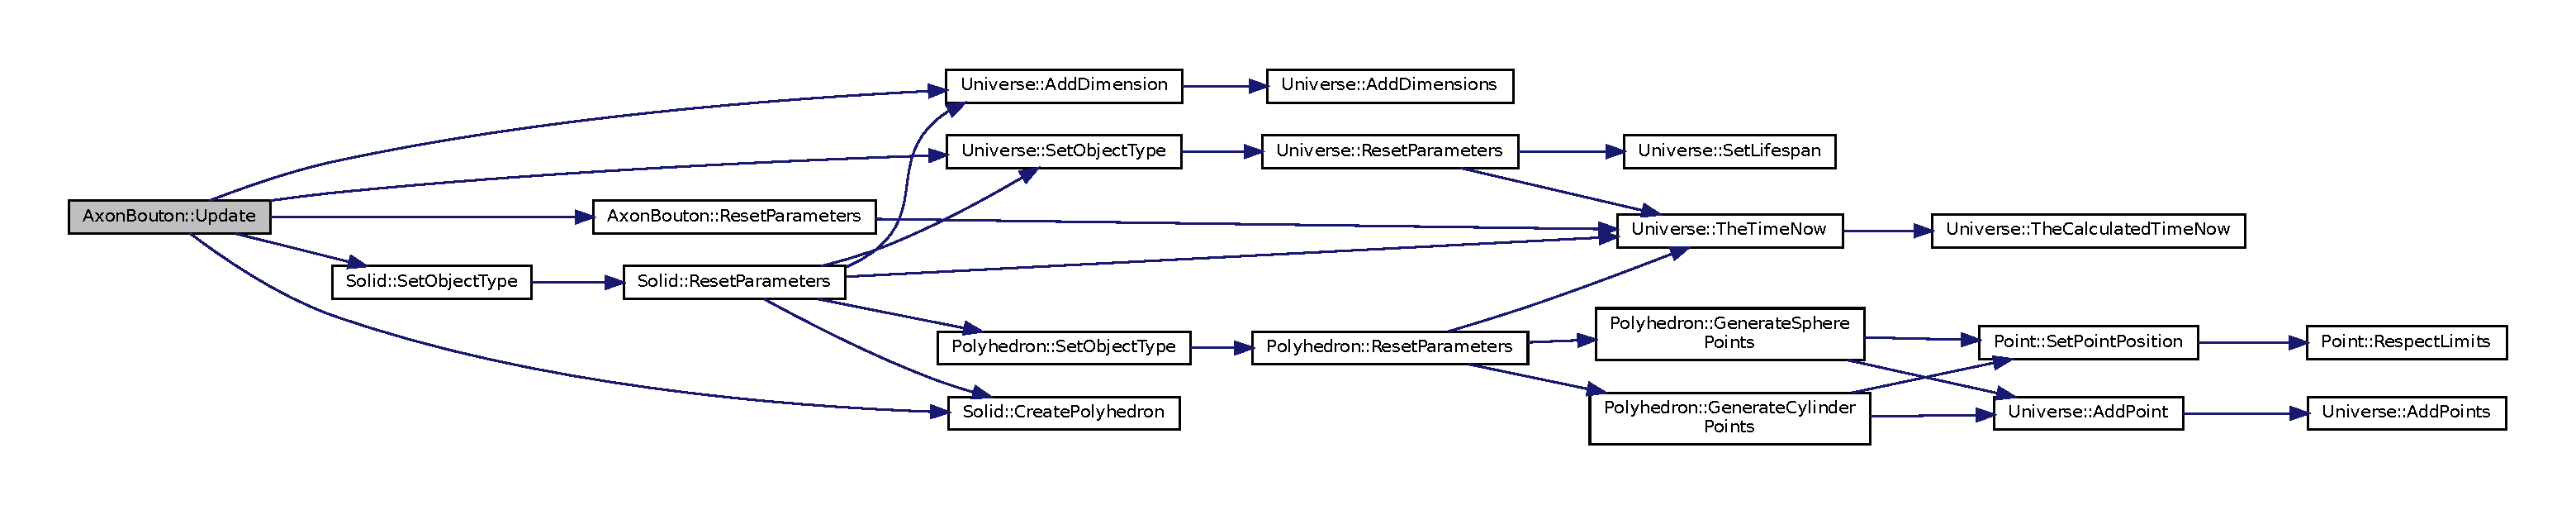
\includegraphics[width=350pt]{class_axon_bouton_a26f89bac681b8f0894fe1ae249733917_cgraph}
\end{center}
\end{figure}


\subsection{Member Data Documentation}
\mbox{\Hypertarget{class_axon_bouton_ad5b4e9b5fefb2ad9e6dfe5ad91be2dd7}\label{class_axon_bouton_ad5b4e9b5fefb2ad9e6dfe5ad91be2dd7}} 
\index{Axon\+Bouton@{Axon\+Bouton}!synapticvesicle\+\_\+list@{synapticvesicle\+\_\+list}}
\index{synapticvesicle\+\_\+list@{synapticvesicle\+\_\+list}!Axon\+Bouton@{Axon\+Bouton}}
\subsubsection{\texorpdfstring{synapticvesicle\+\_\+list}{synapticvesicle\_list}}
{\footnotesize\ttfamily std\+::vector$<$\mbox{\hyperlink{class_axon_bouton}{Axon\+Bouton}}$\ast$$>$ Axon\+Bouton\+::synapticvesicle\+\_\+list\hspace{0.3cm}{\ttfamily [protected]}}



Definition at line 79 of file axonbouton.\+h.



The documentation for this class was generated from the following files\+:\begin{DoxyCompactItemize}
\item 
Brain\+Harmonics/\mbox{\hyperlink{axonbouton_8h}{axonbouton.\+h}}\item 
Brain\+Harmonics/\mbox{\hyperlink{axonbouton_8cc}{axonbouton.\+cc}}\end{DoxyCompactItemize}

\hypertarget{class_axon_branch}{}\section{Axon\+Branch Class Reference}
\label{class_axon_branch}\index{Axon\+Branch@{Axon\+Branch}}


{\ttfamily \#include $<$axonbranch.\+h$>$}



Inheritance diagram for Axon\+Branch\+:\nopagebreak
\begin{figure}[H]
\begin{center}
\leavevmode
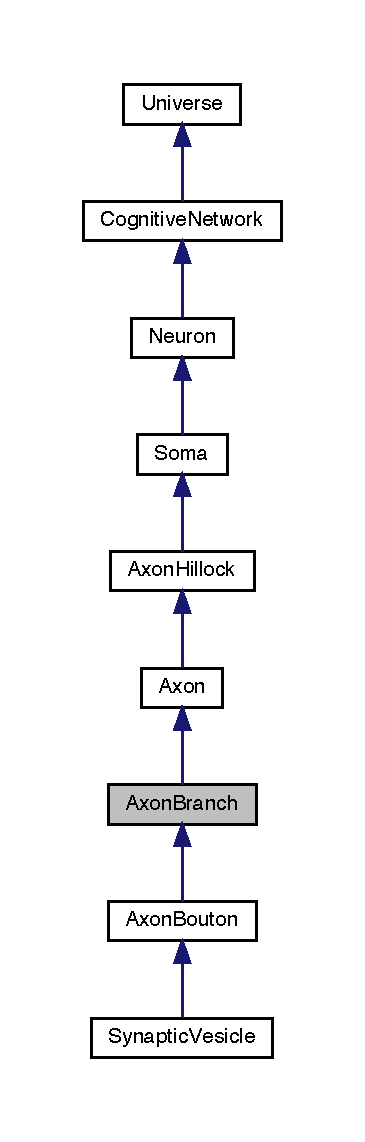
\includegraphics[width=175pt]{class_axon_branch__inherit__graph}
\end{center}
\end{figure}


Collaboration diagram for Axon\+Branch\+:\nopagebreak
\begin{figure}[H]
\begin{center}
\leavevmode
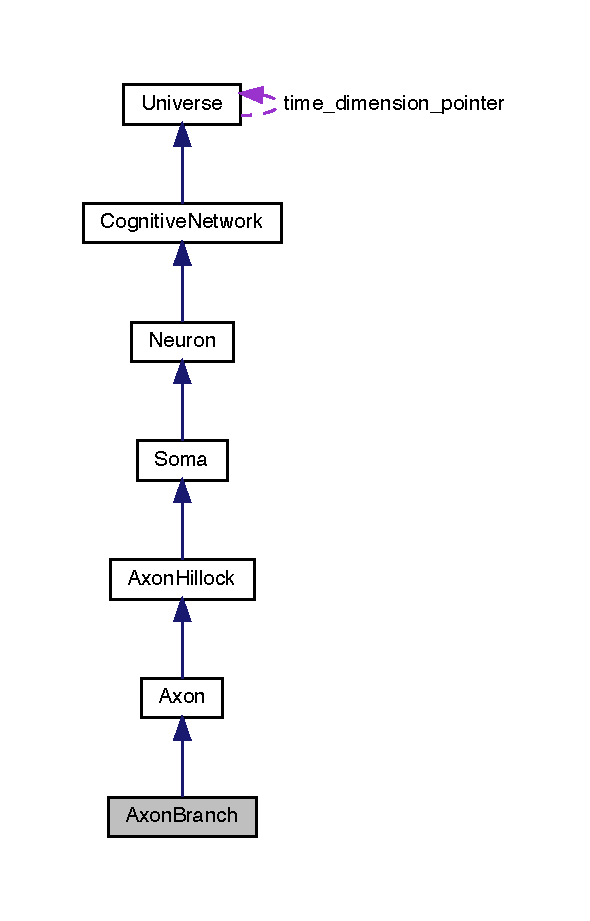
\includegraphics[width=283pt]{class_axon_branch__coll__graph}
\end{center}
\end{figure}
\subsection*{Public Member Functions}
\begin{DoxyCompactItemize}
\item 
\mbox{\hyperlink{class_axon_branch_a5bb6ccef8d94c937a85148af932221c0}{Axon\+Branch}} ()
\item 
\mbox{\hyperlink{class_axon_branch_a67618605ac3731556ab48a6583e21ba8}{Axon\+Branch}} (unsigned int object\+\_\+type)
\item 
\mbox{\hyperlink{class_axon_branch_ad6191fcfd8bedc058a4f1cfb5056f5b2}{Axon\+Branch}} (unsigned int object\+\_\+type, std\+::chrono\+::time\+\_\+point$<$ \mbox{\hyperlink{universe_8h_a0ef8d951d1ca5ab3cfaf7ab4c7a6fd80}{Clock}} $>$ event\+\_\+time)
\item 
\mbox{\hyperlink{class_axon_branch_a98f33462edf82dacab750d1140172912}{Axon\+Branch}} (unsigned int object\+\_\+type, std\+::chrono\+::time\+\_\+point$<$ \mbox{\hyperlink{universe_8h_a0ef8d951d1ca5ab3cfaf7ab4c7a6fd80}{Clock}} $>$ event\+\_\+time, \mbox{\hyperlink{class_axon}{Axon}} \&axon\+\_\+connector)
\item 
virtual \mbox{\hyperlink{class_axon_branch_ae4ef4c954b43d084cafb30cf900a1728}{$\sim$\+Axon\+Branch}} ()
\item 
unsigned int \mbox{\hyperlink{class_axon_branch_a1d2404b68ec2d18a814c96a7c04c5fc4}{Get\+Counter}} (std\+::chrono\+::time\+\_\+point$<$ \mbox{\hyperlink{universe_8h_a0ef8d951d1ca5ab3cfaf7ab4c7a6fd80}{Clock}} $>$ event\+\_\+time)
\item 
double \mbox{\hyperlink{class_axon_branch_a688ec51cd5116e9aebe9b4d3c5c7f2b1}{Get\+Energy}} (std\+::chrono\+::time\+\_\+point$<$ \mbox{\hyperlink{universe_8h_a0ef8d951d1ca5ab3cfaf7ab4c7a6fd80}{Clock}} $>$ event\+\_\+time)
\item 
\mbox{\hyperlink{glad_8h_a950fc91edb4504f62f1c577bf4727c29}{void}} \mbox{\hyperlink{class_axon_branch_a96ba30b18627563d637d4e02fac943be}{Set\+Counter}} (std\+::chrono\+::time\+\_\+point$<$ \mbox{\hyperlink{universe_8h_a0ef8d951d1ca5ab3cfaf7ab4c7a6fd80}{Clock}} $>$ event\+\_\+time, unsigned int \mbox{\hyperlink{glad_8h_a26942fd2ed566ef553eae82d2c109c8f}{val}})
\item 
\mbox{\hyperlink{glad_8h_a950fc91edb4504f62f1c577bf4727c29}{void}} \mbox{\hyperlink{class_axon_branch_a6918dcaf6d9325a1a22a2e6c65ad5dab}{Set\+Energy}} (std\+::chrono\+::time\+\_\+point$<$ \mbox{\hyperlink{universe_8h_a0ef8d951d1ca5ab3cfaf7ab4c7a6fd80}{Clock}} $>$ event\+\_\+time, double \mbox{\hyperlink{glad_8h_a26942fd2ed566ef553eae82d2c109c8f}{val}})
\item 
bool \mbox{\hyperlink{class_axon_branch_a195d68dffd37317db3f94e1b4c8f73c7}{Reset\+Parameters}} (std\+::chrono\+::time\+\_\+point$<$ \mbox{\hyperlink{universe_8h_a0ef8d951d1ca5ab3cfaf7ab4c7a6fd80}{Clock}} $>$ event\+\_\+time)
\item 
\mbox{\hyperlink{class_axon_branch}{Axon\+Branch}} $\ast$ \mbox{\hyperlink{class_axon_branch_a30b4602e5dd121666478ff9de52d022b}{Create\+Axon\+Bouton}} (std\+::chrono\+::time\+\_\+point$<$ \mbox{\hyperlink{universe_8h_a0ef8d951d1ca5ab3cfaf7ab4c7a6fd80}{Clock}} $>$ event\+\_\+time)
\item 
std\+::vector$<$ \mbox{\hyperlink{class_axon_branch}{Axon\+Branch}} $\ast$ $>$ \mbox{\hyperlink{class_axon_branch_a77e93626a7993f76e689d09721974e90}{Create\+Axon\+Boutons}} (std\+::chrono\+::time\+\_\+point$<$ \mbox{\hyperlink{universe_8h_a0ef8d951d1ca5ab3cfaf7ab4c7a6fd80}{Clock}} $>$ event\+\_\+time, int quantity)
\item 
\mbox{\hyperlink{class_axon_branch}{Axon\+Branch}} $\ast$ \mbox{\hyperlink{class_axon_branch_ae861207a8a0aeb2b60c305b25248e4b9}{Clone\+Axon\+Bouton}} (std\+::chrono\+::time\+\_\+point$<$ \mbox{\hyperlink{universe_8h_a0ef8d951d1ca5ab3cfaf7ab4c7a6fd80}{Clock}} $>$ event\+\_\+time, \mbox{\hyperlink{class_axon_branch}{Axon\+Branch}} $\ast$clone\+\_\+object, double perfection\+\_\+membership)
\item 
std\+::vector$<$ \mbox{\hyperlink{class_axon_branch}{Axon\+Branch}} $\ast$ $>$ \mbox{\hyperlink{class_axon_branch_a842b3875b2771f4b8e7316bfb9af894c}{Clone\+Axon\+Boutons}} (std\+::chrono\+::time\+\_\+point$<$ \mbox{\hyperlink{universe_8h_a0ef8d951d1ca5ab3cfaf7ab4c7a6fd80}{Clock}} $>$ event\+\_\+time, std\+::vector$<$ \mbox{\hyperlink{class_axon_branch}{Axon\+Branch}} $\ast$$>$ cloning\+\_\+list, double perfection\+\_\+membership)
\item 
\mbox{\hyperlink{class_axon_branch}{Axon\+Branch}} $\ast$ \mbox{\hyperlink{class_axon_branch_a024c8666555702ebe67e2a5caf1b866a}{Destroy\+Axon\+Bouton}} (std\+::chrono\+::time\+\_\+point$<$ \mbox{\hyperlink{universe_8h_a0ef8d951d1ca5ab3cfaf7ab4c7a6fd80}{Clock}} $>$ event\+\_\+time, \mbox{\hyperlink{class_axon_branch}{Axon\+Branch}} $\ast$destroy\+\_\+object)
\item 
std\+::vector$<$ \mbox{\hyperlink{class_axon_branch}{Axon\+Branch}} $\ast$ $>$ \mbox{\hyperlink{class_axon_branch_a8c022977e091b8cab367b21c0c4930ea}{Destroy\+Axon\+Boutons}} (std\+::chrono\+::time\+\_\+point$<$ \mbox{\hyperlink{universe_8h_a0ef8d951d1ca5ab3cfaf7ab4c7a6fd80}{Clock}} $>$ event\+\_\+time, std\+::vector$<$ \mbox{\hyperlink{class_axon_branch}{Axon\+Branch}} $\ast$$>$ destruction\+\_\+list)
\item 
\mbox{\hyperlink{class_axon_branch}{Axon\+Branch}} $\ast$ \mbox{\hyperlink{class_axon_branch_a88e6af84b45bb6f6f8900a6d4aec446c}{Add\+Axon\+Bouton}} (std\+::chrono\+::time\+\_\+point$<$ \mbox{\hyperlink{universe_8h_a0ef8d951d1ca5ab3cfaf7ab4c7a6fd80}{Clock}} $>$ event\+\_\+time, \mbox{\hyperlink{class_axon_branch}{Axon\+Branch}} $\ast$add\+\_\+object)
\item 
std\+::vector$<$ \mbox{\hyperlink{class_axon_branch}{Axon\+Branch}} $\ast$ $>$ \mbox{\hyperlink{class_axon_branch_a788ca8cc7e6f60f07b9e19a8e3022b64}{Add\+Axon\+Boutons}} (std\+::chrono\+::time\+\_\+point$<$ \mbox{\hyperlink{universe_8h_a0ef8d951d1ca5ab3cfaf7ab4c7a6fd80}{Clock}} $>$ event\+\_\+time, std\+::vector$<$ \mbox{\hyperlink{class_axon_branch}{Axon\+Branch}} $\ast$$>$ add\+\_\+objects)
\item 
\mbox{\hyperlink{class_axon_branch}{Axon\+Branch}} $\ast$ \mbox{\hyperlink{class_axon_branch_a06753a2a61941a59d86510e51ba44b15}{Remove\+Axon\+Bouton}} (std\+::chrono\+::time\+\_\+point$<$ \mbox{\hyperlink{universe_8h_a0ef8d951d1ca5ab3cfaf7ab4c7a6fd80}{Clock}} $>$ event\+\_\+time)
\item 
std\+::vector$<$ \mbox{\hyperlink{class_axon_branch}{Axon\+Branch}} $\ast$ $>$ \mbox{\hyperlink{class_axon_branch_a815e055e37f89fb2627b250c5b95d406}{Remove\+Axon\+Boutons}} (std\+::chrono\+::time\+\_\+point$<$ \mbox{\hyperlink{universe_8h_a0ef8d951d1ca5ab3cfaf7ab4c7a6fd80}{Clock}} $>$ event\+\_\+time, int quantity)
\item 
\mbox{\hyperlink{class_axon_branch}{Axon\+Branch}} $\ast$ \mbox{\hyperlink{class_axon_branch_a6fa6eea91e72fd142f3d691f7ca4c99a}{Get\+Axon\+Bouton}} (std\+::chrono\+::time\+\_\+point$<$ \mbox{\hyperlink{universe_8h_a0ef8d951d1ca5ab3cfaf7ab4c7a6fd80}{Clock}} $>$ event\+\_\+time, int selector)
\item 
std\+::vector$<$ \mbox{\hyperlink{class_axon_branch}{Axon\+Branch}} $\ast$ $>$ \mbox{\hyperlink{class_axon_branch_aafadba57924686a8087c7f7758889045}{Get\+Axon\+Boutons}} (std\+::chrono\+::time\+\_\+point$<$ \mbox{\hyperlink{universe_8h_a0ef8d951d1ca5ab3cfaf7ab4c7a6fd80}{Clock}} $>$ event\+\_\+time)
\item 
int \mbox{\hyperlink{class_axon_branch_a6e434a57873ab0fdbc72cf7ecc7228ed}{Growth}} (std\+::chrono\+::time\+\_\+point$<$ \mbox{\hyperlink{universe_8h_a0ef8d951d1ca5ab3cfaf7ab4c7a6fd80}{Clock}} $>$ event\+\_\+time)
\item 
int \mbox{\hyperlink{class_axon_branch_a5a80bcccdc2be9f77fca25131937b52f}{Update}} (std\+::chrono\+::time\+\_\+point$<$ std\+::chrono\+::high\+\_\+resolution\+\_\+clock $>$ \mbox{\hyperlink{glad_8h_a26942fd2ed566ef553eae82d2c109c8f}{val}})
\end{DoxyCompactItemize}
\subsection*{Protected Attributes}
\begin{DoxyCompactItemize}
\item 
std\+::vector$<$ \mbox{\hyperlink{class_axon_branch}{Axon\+Branch}} $\ast$ $>$ \mbox{\hyperlink{class_axon_branch_a43224f9fcb62274709438c9833cb10e5}{axonbouton\+\_\+list}}
\end{DoxyCompactItemize}
\subsection*{Additional Inherited Members}


\subsection{Detailed Description}


Definition at line 14 of file axonbranch.\+h.



\subsection{Constructor \& Destructor Documentation}
\mbox{\Hypertarget{class_axon_branch_a5bb6ccef8d94c937a85148af932221c0}\label{class_axon_branch_a5bb6ccef8d94c937a85148af932221c0}} 
\index{Axon\+Branch@{Axon\+Branch}!Axon\+Branch@{Axon\+Branch}}
\index{Axon\+Branch@{Axon\+Branch}!Axon\+Branch@{Axon\+Branch}}
\subsubsection{\texorpdfstring{Axon\+Branch()}{AxonBranch()}\hspace{0.1cm}{\footnotesize\ttfamily [1/4]}}
{\footnotesize\ttfamily Axon\+Branch\+::\+Axon\+Branch (\begin{DoxyParamCaption}{ }\end{DoxyParamCaption})\hspace{0.3cm}{\ttfamily [inline]}}



Definition at line 17 of file axonbranch.\+h.

\mbox{\Hypertarget{class_axon_branch_a67618605ac3731556ab48a6583e21ba8}\label{class_axon_branch_a67618605ac3731556ab48a6583e21ba8}} 
\index{Axon\+Branch@{Axon\+Branch}!Axon\+Branch@{Axon\+Branch}}
\index{Axon\+Branch@{Axon\+Branch}!Axon\+Branch@{Axon\+Branch}}
\subsubsection{\texorpdfstring{Axon\+Branch()}{AxonBranch()}\hspace{0.1cm}{\footnotesize\ttfamily [2/4]}}
{\footnotesize\ttfamily Axon\+Branch\+::\+Axon\+Branch (\begin{DoxyParamCaption}\item[{unsigned int}]{object\+\_\+type }\end{DoxyParamCaption})\hspace{0.3cm}{\ttfamily [inline]}}



Definition at line 19 of file axonbranch.\+h.

\mbox{\Hypertarget{class_axon_branch_ad6191fcfd8bedc058a4f1cfb5056f5b2}\label{class_axon_branch_ad6191fcfd8bedc058a4f1cfb5056f5b2}} 
\index{Axon\+Branch@{Axon\+Branch}!Axon\+Branch@{Axon\+Branch}}
\index{Axon\+Branch@{Axon\+Branch}!Axon\+Branch@{Axon\+Branch}}
\subsubsection{\texorpdfstring{Axon\+Branch()}{AxonBranch()}\hspace{0.1cm}{\footnotesize\ttfamily [3/4]}}
{\footnotesize\ttfamily Axon\+Branch\+::\+Axon\+Branch (\begin{DoxyParamCaption}\item[{unsigned int}]{object\+\_\+type,  }\item[{std\+::chrono\+::time\+\_\+point$<$ \mbox{\hyperlink{universe_8h_a0ef8d951d1ca5ab3cfaf7ab4c7a6fd80}{Clock}} $>$}]{event\+\_\+time }\end{DoxyParamCaption})\hspace{0.3cm}{\ttfamily [inline]}}



Definition at line 21 of file axonbranch.\+h.

\mbox{\Hypertarget{class_axon_branch_a98f33462edf82dacab750d1140172912}\label{class_axon_branch_a98f33462edf82dacab750d1140172912}} 
\index{Axon\+Branch@{Axon\+Branch}!Axon\+Branch@{Axon\+Branch}}
\index{Axon\+Branch@{Axon\+Branch}!Axon\+Branch@{Axon\+Branch}}
\subsubsection{\texorpdfstring{Axon\+Branch()}{AxonBranch()}\hspace{0.1cm}{\footnotesize\ttfamily [4/4]}}
{\footnotesize\ttfamily Axon\+Branch\+::\+Axon\+Branch (\begin{DoxyParamCaption}\item[{unsigned int}]{object\+\_\+type,  }\item[{std\+::chrono\+::time\+\_\+point$<$ \mbox{\hyperlink{universe_8h_a0ef8d951d1ca5ab3cfaf7ab4c7a6fd80}{Clock}} $>$}]{event\+\_\+time,  }\item[{\mbox{\hyperlink{class_axon}{Axon}} \&}]{axon\+\_\+connector }\end{DoxyParamCaption})\hspace{0.3cm}{\ttfamily [inline]}}



Definition at line 23 of file axonbranch.\+h.

Here is the call graph for this function\+:\nopagebreak
\begin{figure}[H]
\begin{center}
\leavevmode
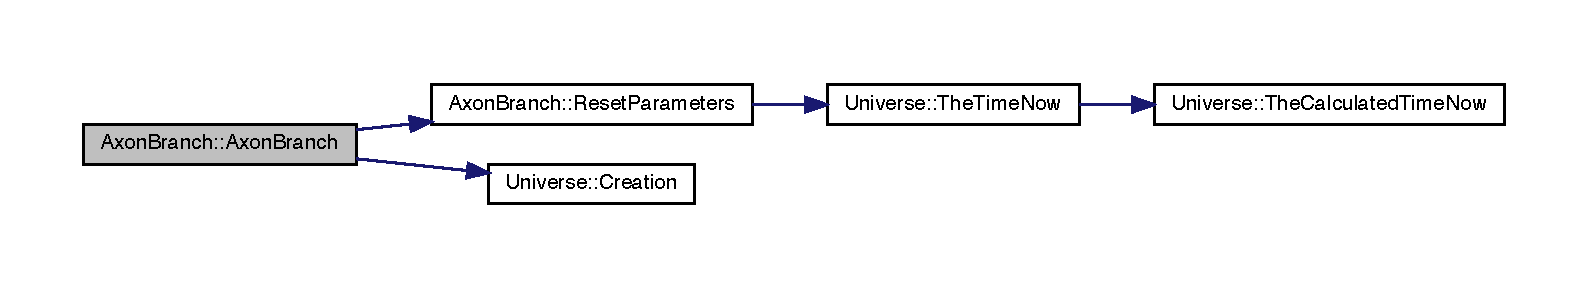
\includegraphics[width=350pt]{class_axon_branch_a98f33462edf82dacab750d1140172912_cgraph}
\end{center}
\end{figure}
\mbox{\Hypertarget{class_axon_branch_ae4ef4c954b43d084cafb30cf900a1728}\label{class_axon_branch_ae4ef4c954b43d084cafb30cf900a1728}} 
\index{Axon\+Branch@{Axon\+Branch}!````~Axon\+Branch@{$\sim$\+Axon\+Branch}}
\index{````~Axon\+Branch@{$\sim$\+Axon\+Branch}!Axon\+Branch@{Axon\+Branch}}
\subsubsection{\texorpdfstring{$\sim$\+Axon\+Branch()}{~AxonBranch()}}
{\footnotesize\ttfamily virtual Axon\+Branch\+::$\sim$\+Axon\+Branch (\begin{DoxyParamCaption}{ }\end{DoxyParamCaption})\hspace{0.3cm}{\ttfamily [inline]}, {\ttfamily [virtual]}}

Default destructor 

Definition at line 36 of file axonbranch.\+h.



\subsection{Member Function Documentation}
\mbox{\Hypertarget{class_axon_branch_a88e6af84b45bb6f6f8900a6d4aec446c}\label{class_axon_branch_a88e6af84b45bb6f6f8900a6d4aec446c}} 
\index{Axon\+Branch@{Axon\+Branch}!Add\+Axon\+Bouton@{Add\+Axon\+Bouton}}
\index{Add\+Axon\+Bouton@{Add\+Axon\+Bouton}!Axon\+Branch@{Axon\+Branch}}
\subsubsection{\texorpdfstring{Add\+Axon\+Bouton()}{AddAxonBouton()}}
{\footnotesize\ttfamily \mbox{\hyperlink{class_axon_branch}{Axon\+Branch}} $\ast$ Axon\+Branch\+::\+Add\+Axon\+Bouton (\begin{DoxyParamCaption}\item[{std\+::chrono\+::time\+\_\+point$<$ \mbox{\hyperlink{universe_8h_a0ef8d951d1ca5ab3cfaf7ab4c7a6fd80}{Clock}} $>$}]{event\+\_\+time,  }\item[{\mbox{\hyperlink{class_axon_branch}{Axon\+Branch}} $\ast$}]{add\+\_\+object }\end{DoxyParamCaption})}



Definition at line 115 of file axonbranch.\+cc.

Here is the caller graph for this function\+:\nopagebreak
\begin{figure}[H]
\begin{center}
\leavevmode
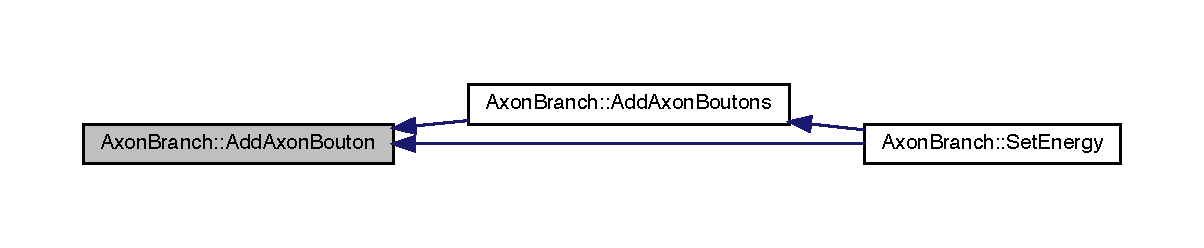
\includegraphics[width=350pt]{class_axon_branch_a88e6af84b45bb6f6f8900a6d4aec446c_icgraph}
\end{center}
\end{figure}
\mbox{\Hypertarget{class_axon_branch_a788ca8cc7e6f60f07b9e19a8e3022b64}\label{class_axon_branch_a788ca8cc7e6f60f07b9e19a8e3022b64}} 
\index{Axon\+Branch@{Axon\+Branch}!Add\+Axon\+Boutons@{Add\+Axon\+Boutons}}
\index{Add\+Axon\+Boutons@{Add\+Axon\+Boutons}!Axon\+Branch@{Axon\+Branch}}
\subsubsection{\texorpdfstring{Add\+Axon\+Boutons()}{AddAxonBoutons()}}
{\footnotesize\ttfamily std\+::vector$<$ \mbox{\hyperlink{class_axon_branch}{Axon\+Branch}} $\ast$ $>$ Axon\+Branch\+::\+Add\+Axon\+Boutons (\begin{DoxyParamCaption}\item[{std\+::chrono\+::time\+\_\+point$<$ \mbox{\hyperlink{universe_8h_a0ef8d951d1ca5ab3cfaf7ab4c7a6fd80}{Clock}} $>$}]{event\+\_\+time,  }\item[{std\+::vector$<$ \mbox{\hyperlink{class_axon_branch}{Axon\+Branch}} $\ast$$>$}]{add\+\_\+objects }\end{DoxyParamCaption})}



Definition at line 126 of file axonbranch.\+cc.

Here is the call graph for this function\+:\nopagebreak
\begin{figure}[H]
\begin{center}
\leavevmode
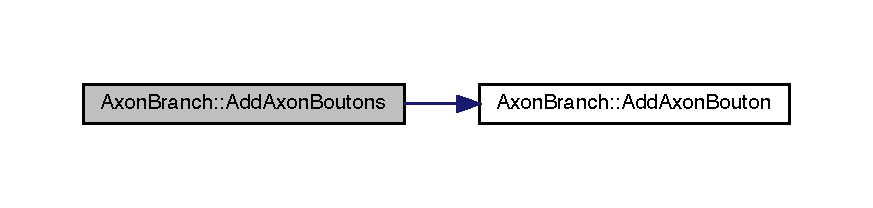
\includegraphics[width=350pt]{class_axon_branch_a788ca8cc7e6f60f07b9e19a8e3022b64_cgraph}
\end{center}
\end{figure}
\mbox{\Hypertarget{class_axon_branch_ae861207a8a0aeb2b60c305b25248e4b9}\label{class_axon_branch_ae861207a8a0aeb2b60c305b25248e4b9}} 
\index{Axon\+Branch@{Axon\+Branch}!Clone\+Axon\+Bouton@{Clone\+Axon\+Bouton}}
\index{Clone\+Axon\+Bouton@{Clone\+Axon\+Bouton}!Axon\+Branch@{Axon\+Branch}}
\subsubsection{\texorpdfstring{Clone\+Axon\+Bouton()}{CloneAxonBouton()}}
{\footnotesize\ttfamily \mbox{\hyperlink{class_axon_branch}{Axon\+Branch}} $\ast$ Axon\+Branch\+::\+Clone\+Axon\+Bouton (\begin{DoxyParamCaption}\item[{std\+::chrono\+::time\+\_\+point$<$ \mbox{\hyperlink{universe_8h_a0ef8d951d1ca5ab3cfaf7ab4c7a6fd80}{Clock}} $>$}]{event\+\_\+time,  }\item[{\mbox{\hyperlink{class_axon_branch}{Axon\+Branch}} $\ast$}]{clone\+\_\+object,  }\item[{double}]{perfection\+\_\+membership }\end{DoxyParamCaption})}



Definition at line 100 of file axonbranch.\+cc.

\mbox{\Hypertarget{class_axon_branch_a842b3875b2771f4b8e7316bfb9af894c}\label{class_axon_branch_a842b3875b2771f4b8e7316bfb9af894c}} 
\index{Axon\+Branch@{Axon\+Branch}!Clone\+Axon\+Boutons@{Clone\+Axon\+Boutons}}
\index{Clone\+Axon\+Boutons@{Clone\+Axon\+Boutons}!Axon\+Branch@{Axon\+Branch}}
\subsubsection{\texorpdfstring{Clone\+Axon\+Boutons()}{CloneAxonBoutons()}}
{\footnotesize\ttfamily std\+::vector$<$ \mbox{\hyperlink{class_axon_branch}{Axon\+Branch}} $\ast$ $>$ Axon\+Branch\+::\+Clone\+Axon\+Boutons (\begin{DoxyParamCaption}\item[{std\+::chrono\+::time\+\_\+point$<$ \mbox{\hyperlink{universe_8h_a0ef8d951d1ca5ab3cfaf7ab4c7a6fd80}{Clock}} $>$}]{event\+\_\+time,  }\item[{std\+::vector$<$ \mbox{\hyperlink{class_axon_branch}{Axon\+Branch}} $\ast$$>$}]{cloning\+\_\+list,  }\item[{double}]{perfection\+\_\+membership }\end{DoxyParamCaption})}



Definition at line 95 of file axonbranch.\+cc.

\mbox{\Hypertarget{class_axon_branch_a30b4602e5dd121666478ff9de52d022b}\label{class_axon_branch_a30b4602e5dd121666478ff9de52d022b}} 
\index{Axon\+Branch@{Axon\+Branch}!Create\+Axon\+Bouton@{Create\+Axon\+Bouton}}
\index{Create\+Axon\+Bouton@{Create\+Axon\+Bouton}!Axon\+Branch@{Axon\+Branch}}
\subsubsection{\texorpdfstring{Create\+Axon\+Bouton()}{CreateAxonBouton()}}
{\footnotesize\ttfamily \mbox{\hyperlink{class_axon_branch}{Axon\+Branch}} $\ast$ Axon\+Branch\+::\+Create\+Axon\+Bouton (\begin{DoxyParamCaption}\item[{std\+::chrono\+::time\+\_\+point$<$ \mbox{\hyperlink{universe_8h_a0ef8d951d1ca5ab3cfaf7ab4c7a6fd80}{Clock}} $>$}]{event\+\_\+time }\end{DoxyParamCaption})}



Definition at line 62 of file axonbranch.\+cc.

Here is the caller graph for this function\+:\nopagebreak
\begin{figure}[H]
\begin{center}
\leavevmode
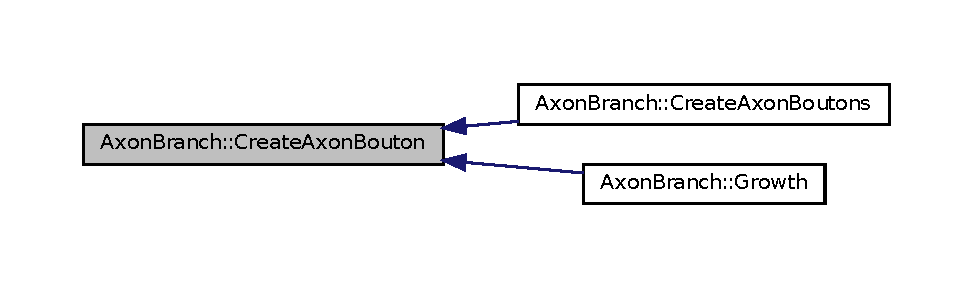
\includegraphics[width=350pt]{class_axon_branch_a30b4602e5dd121666478ff9de52d022b_icgraph}
\end{center}
\end{figure}
\mbox{\Hypertarget{class_axon_branch_a77e93626a7993f76e689d09721974e90}\label{class_axon_branch_a77e93626a7993f76e689d09721974e90}} 
\index{Axon\+Branch@{Axon\+Branch}!Create\+Axon\+Boutons@{Create\+Axon\+Boutons}}
\index{Create\+Axon\+Boutons@{Create\+Axon\+Boutons}!Axon\+Branch@{Axon\+Branch}}
\subsubsection{\texorpdfstring{Create\+Axon\+Boutons()}{CreateAxonBoutons()}}
{\footnotesize\ttfamily std\+::vector$<$ \mbox{\hyperlink{class_axon_branch}{Axon\+Branch}} $\ast$ $>$ Axon\+Branch\+::\+Create\+Axon\+Boutons (\begin{DoxyParamCaption}\item[{std\+::chrono\+::time\+\_\+point$<$ \mbox{\hyperlink{universe_8h_a0ef8d951d1ca5ab3cfaf7ab4c7a6fd80}{Clock}} $>$}]{event\+\_\+time,  }\item[{int}]{quantity }\end{DoxyParamCaption})}



Definition at line 73 of file axonbranch.\+cc.

Here is the call graph for this function\+:\nopagebreak
\begin{figure}[H]
\begin{center}
\leavevmode
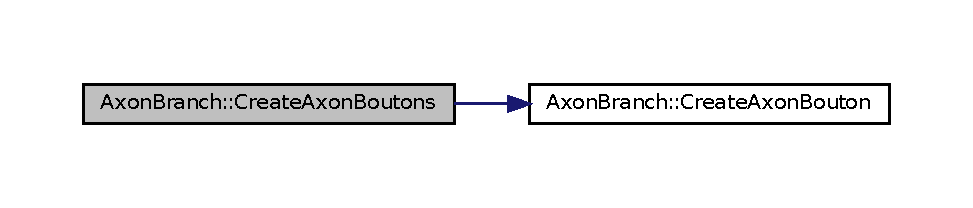
\includegraphics[width=350pt]{class_axon_branch_a77e93626a7993f76e689d09721974e90_cgraph}
\end{center}
\end{figure}
\mbox{\Hypertarget{class_axon_branch_a024c8666555702ebe67e2a5caf1b866a}\label{class_axon_branch_a024c8666555702ebe67e2a5caf1b866a}} 
\index{Axon\+Branch@{Axon\+Branch}!Destroy\+Axon\+Bouton@{Destroy\+Axon\+Bouton}}
\index{Destroy\+Axon\+Bouton@{Destroy\+Axon\+Bouton}!Axon\+Branch@{Axon\+Branch}}
\subsubsection{\texorpdfstring{Destroy\+Axon\+Bouton()}{DestroyAxonBouton()}}
{\footnotesize\ttfamily \mbox{\hyperlink{class_axon_branch}{Axon\+Branch}} $\ast$ Axon\+Branch\+::\+Destroy\+Axon\+Bouton (\begin{DoxyParamCaption}\item[{std\+::chrono\+::time\+\_\+point$<$ \mbox{\hyperlink{universe_8h_a0ef8d951d1ca5ab3cfaf7ab4c7a6fd80}{Clock}} $>$}]{event\+\_\+time,  }\item[{\mbox{\hyperlink{class_axon_branch}{Axon\+Branch}} $\ast$}]{destroy\+\_\+object }\end{DoxyParamCaption})}



Definition at line 110 of file axonbranch.\+cc.

\mbox{\Hypertarget{class_axon_branch_a8c022977e091b8cab367b21c0c4930ea}\label{class_axon_branch_a8c022977e091b8cab367b21c0c4930ea}} 
\index{Axon\+Branch@{Axon\+Branch}!Destroy\+Axon\+Boutons@{Destroy\+Axon\+Boutons}}
\index{Destroy\+Axon\+Boutons@{Destroy\+Axon\+Boutons}!Axon\+Branch@{Axon\+Branch}}
\subsubsection{\texorpdfstring{Destroy\+Axon\+Boutons()}{DestroyAxonBoutons()}}
{\footnotesize\ttfamily std\+::vector$<$ \mbox{\hyperlink{class_axon_branch}{Axon\+Branch}} $\ast$ $>$ Axon\+Branch\+::\+Destroy\+Axon\+Boutons (\begin{DoxyParamCaption}\item[{std\+::chrono\+::time\+\_\+point$<$ \mbox{\hyperlink{universe_8h_a0ef8d951d1ca5ab3cfaf7ab4c7a6fd80}{Clock}} $>$}]{event\+\_\+time,  }\item[{std\+::vector$<$ \mbox{\hyperlink{class_axon_branch}{Axon\+Branch}} $\ast$$>$}]{destruction\+\_\+list }\end{DoxyParamCaption})}



Definition at line 105 of file axonbranch.\+cc.

\mbox{\Hypertarget{class_axon_branch_a6fa6eea91e72fd142f3d691f7ca4c99a}\label{class_axon_branch_a6fa6eea91e72fd142f3d691f7ca4c99a}} 
\index{Axon\+Branch@{Axon\+Branch}!Get\+Axon\+Bouton@{Get\+Axon\+Bouton}}
\index{Get\+Axon\+Bouton@{Get\+Axon\+Bouton}!Axon\+Branch@{Axon\+Branch}}
\subsubsection{\texorpdfstring{Get\+Axon\+Bouton()}{GetAxonBouton()}}
{\footnotesize\ttfamily \mbox{\hyperlink{class_axon_branch}{Axon\+Branch}} $\ast$ Axon\+Branch\+::\+Get\+Axon\+Bouton (\begin{DoxyParamCaption}\item[{std\+::chrono\+::time\+\_\+point$<$ \mbox{\hyperlink{universe_8h_a0ef8d951d1ca5ab3cfaf7ab4c7a6fd80}{Clock}} $>$}]{event\+\_\+time,  }\item[{int}]{selector }\end{DoxyParamCaption})}



Definition at line 159 of file axonbranch.\+cc.

\mbox{\Hypertarget{class_axon_branch_aafadba57924686a8087c7f7758889045}\label{class_axon_branch_aafadba57924686a8087c7f7758889045}} 
\index{Axon\+Branch@{Axon\+Branch}!Get\+Axon\+Boutons@{Get\+Axon\+Boutons}}
\index{Get\+Axon\+Boutons@{Get\+Axon\+Boutons}!Axon\+Branch@{Axon\+Branch}}
\subsubsection{\texorpdfstring{Get\+Axon\+Boutons()}{GetAxonBoutons()}}
{\footnotesize\ttfamily std\+::vector$<$ \mbox{\hyperlink{class_axon_branch}{Axon\+Branch}} $\ast$ $>$ Axon\+Branch\+::\+Get\+Axon\+Boutons (\begin{DoxyParamCaption}\item[{std\+::chrono\+::time\+\_\+point$<$ \mbox{\hyperlink{universe_8h_a0ef8d951d1ca5ab3cfaf7ab4c7a6fd80}{Clock}} $>$}]{event\+\_\+time }\end{DoxyParamCaption})}



Definition at line 164 of file axonbranch.\+cc.

\mbox{\Hypertarget{class_axon_branch_a1d2404b68ec2d18a814c96a7c04c5fc4}\label{class_axon_branch_a1d2404b68ec2d18a814c96a7c04c5fc4}} 
\index{Axon\+Branch@{Axon\+Branch}!Get\+Counter@{Get\+Counter}}
\index{Get\+Counter@{Get\+Counter}!Axon\+Branch@{Axon\+Branch}}
\subsubsection{\texorpdfstring{Get\+Counter()}{GetCounter()}}
{\footnotesize\ttfamily unsigned int Axon\+Branch\+::\+Get\+Counter (\begin{DoxyParamCaption}\item[{std\+::chrono\+::time\+\_\+point$<$ \mbox{\hyperlink{universe_8h_a0ef8d951d1ca5ab3cfaf7ab4c7a6fd80}{Clock}} $>$}]{event\+\_\+time }\end{DoxyParamCaption})\hspace{0.3cm}{\ttfamily [inline]}}



Definition at line 37 of file axonbranch.\+h.

\mbox{\Hypertarget{class_axon_branch_a688ec51cd5116e9aebe9b4d3c5c7f2b1}\label{class_axon_branch_a688ec51cd5116e9aebe9b4d3c5c7f2b1}} 
\index{Axon\+Branch@{Axon\+Branch}!Get\+Energy@{Get\+Energy}}
\index{Get\+Energy@{Get\+Energy}!Axon\+Branch@{Axon\+Branch}}
\subsubsection{\texorpdfstring{Get\+Energy()}{GetEnergy()}}
{\footnotesize\ttfamily double Axon\+Branch\+::\+Get\+Energy (\begin{DoxyParamCaption}\item[{std\+::chrono\+::time\+\_\+point$<$ \mbox{\hyperlink{universe_8h_a0ef8d951d1ca5ab3cfaf7ab4c7a6fd80}{Clock}} $>$}]{event\+\_\+time }\end{DoxyParamCaption})\hspace{0.3cm}{\ttfamily [inline]}}



Definition at line 38 of file axonbranch.\+h.

\mbox{\Hypertarget{class_axon_branch_a6e434a57873ab0fdbc72cf7ecc7228ed}\label{class_axon_branch_a6e434a57873ab0fdbc72cf7ecc7228ed}} 
\index{Axon\+Branch@{Axon\+Branch}!Growth@{Growth}}
\index{Growth@{Growth}!Axon\+Branch@{Axon\+Branch}}
\subsubsection{\texorpdfstring{Growth()}{Growth()}}
{\footnotesize\ttfamily int Axon\+Branch\+::\+Growth (\begin{DoxyParamCaption}\item[{std\+::chrono\+::time\+\_\+point$<$ \mbox{\hyperlink{universe_8h_a0ef8d951d1ca5ab3cfaf7ab4c7a6fd80}{Clock}} $>$}]{event\+\_\+time }\end{DoxyParamCaption})}



Definition at line 169 of file axonbranch.\+cc.

Here is the call graph for this function\+:\nopagebreak
\begin{figure}[H]
\begin{center}
\leavevmode
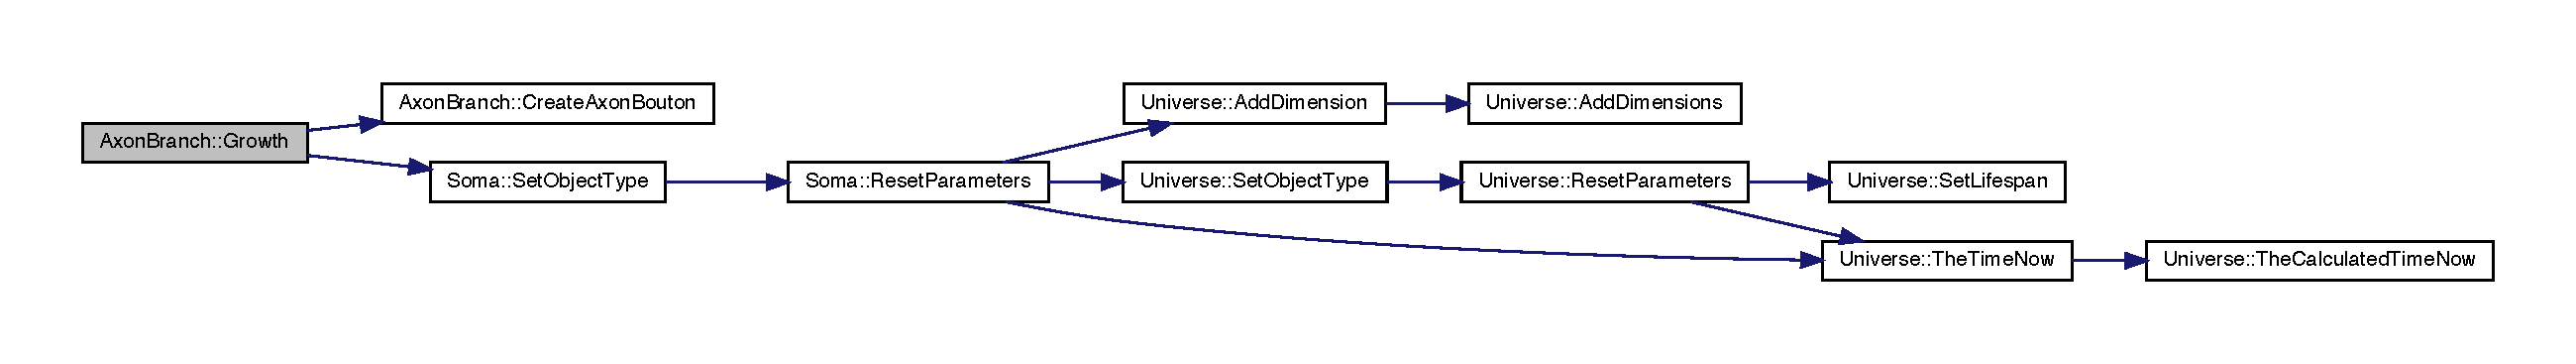
\includegraphics[width=350pt]{class_axon_branch_a6e434a57873ab0fdbc72cf7ecc7228ed_cgraph}
\end{center}
\end{figure}
\mbox{\Hypertarget{class_axon_branch_a06753a2a61941a59d86510e51ba44b15}\label{class_axon_branch_a06753a2a61941a59d86510e51ba44b15}} 
\index{Axon\+Branch@{Axon\+Branch}!Remove\+Axon\+Bouton@{Remove\+Axon\+Bouton}}
\index{Remove\+Axon\+Bouton@{Remove\+Axon\+Bouton}!Axon\+Branch@{Axon\+Branch}}
\subsubsection{\texorpdfstring{Remove\+Axon\+Bouton()}{RemoveAxonBouton()}}
{\footnotesize\ttfamily \mbox{\hyperlink{class_axon_branch}{Axon\+Branch}} $\ast$ Axon\+Branch\+::\+Remove\+Axon\+Bouton (\begin{DoxyParamCaption}\item[{std\+::chrono\+::time\+\_\+point$<$ \mbox{\hyperlink{universe_8h_a0ef8d951d1ca5ab3cfaf7ab4c7a6fd80}{Clock}} $>$}]{event\+\_\+time }\end{DoxyParamCaption})}



Definition at line 148 of file axonbranch.\+cc.

\mbox{\Hypertarget{class_axon_branch_a815e055e37f89fb2627b250c5b95d406}\label{class_axon_branch_a815e055e37f89fb2627b250c5b95d406}} 
\index{Axon\+Branch@{Axon\+Branch}!Remove\+Axon\+Boutons@{Remove\+Axon\+Boutons}}
\index{Remove\+Axon\+Boutons@{Remove\+Axon\+Boutons}!Axon\+Branch@{Axon\+Branch}}
\subsubsection{\texorpdfstring{Remove\+Axon\+Boutons()}{RemoveAxonBoutons()}}
{\footnotesize\ttfamily std\+::vector$<$ \mbox{\hyperlink{class_axon_branch}{Axon\+Branch}} $\ast$ $>$ Axon\+Branch\+::\+Remove\+Axon\+Boutons (\begin{DoxyParamCaption}\item[{std\+::chrono\+::time\+\_\+point$<$ \mbox{\hyperlink{universe_8h_a0ef8d951d1ca5ab3cfaf7ab4c7a6fd80}{Clock}} $>$}]{event\+\_\+time,  }\item[{int}]{quantity }\end{DoxyParamCaption})}



Definition at line 154 of file axonbranch.\+cc.

\mbox{\Hypertarget{class_axon_branch_a195d68dffd37317db3f94e1b4c8f73c7}\label{class_axon_branch_a195d68dffd37317db3f94e1b4c8f73c7}} 
\index{Axon\+Branch@{Axon\+Branch}!Reset\+Parameters@{Reset\+Parameters}}
\index{Reset\+Parameters@{Reset\+Parameters}!Axon\+Branch@{Axon\+Branch}}
\subsubsection{\texorpdfstring{Reset\+Parameters()}{ResetParameters()}}
{\footnotesize\ttfamily bool Axon\+Branch\+::\+Reset\+Parameters (\begin{DoxyParamCaption}\item[{std\+::chrono\+::time\+\_\+point$<$ \mbox{\hyperlink{universe_8h_a0ef8d951d1ca5ab3cfaf7ab4c7a6fd80}{Clock}} $>$}]{event\+\_\+time }\end{DoxyParamCaption})}



Definition at line 20 of file axonbranch.\+cc.

Here is the call graph for this function\+:\nopagebreak
\begin{figure}[H]
\begin{center}
\leavevmode
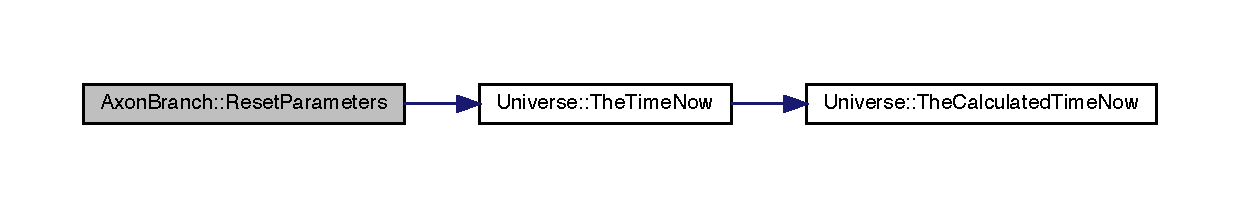
\includegraphics[width=350pt]{class_axon_branch_a195d68dffd37317db3f94e1b4c8f73c7_cgraph}
\end{center}
\end{figure}
Here is the caller graph for this function\+:\nopagebreak
\begin{figure}[H]
\begin{center}
\leavevmode
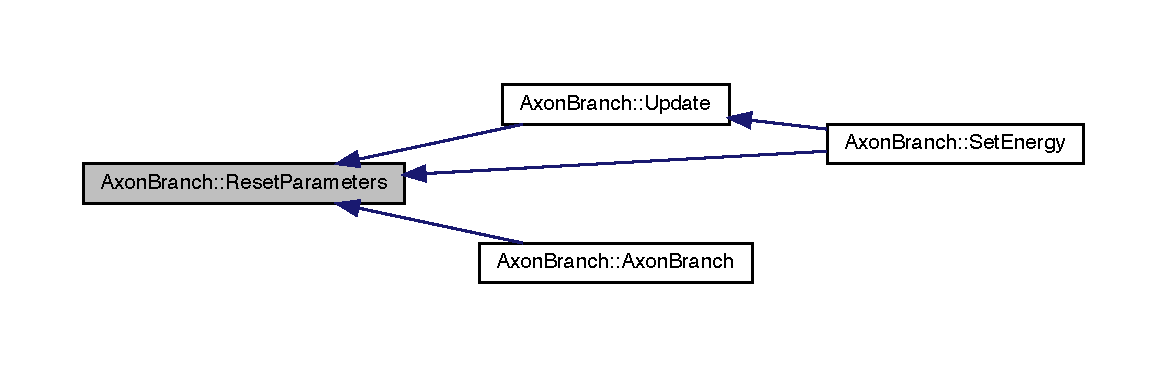
\includegraphics[width=350pt]{class_axon_branch_a195d68dffd37317db3f94e1b4c8f73c7_icgraph}
\end{center}
\end{figure}
\mbox{\Hypertarget{class_axon_branch_a96ba30b18627563d637d4e02fac943be}\label{class_axon_branch_a96ba30b18627563d637d4e02fac943be}} 
\index{Axon\+Branch@{Axon\+Branch}!Set\+Counter@{Set\+Counter}}
\index{Set\+Counter@{Set\+Counter}!Axon\+Branch@{Axon\+Branch}}
\subsubsection{\texorpdfstring{Set\+Counter()}{SetCounter()}}
{\footnotesize\ttfamily \mbox{\hyperlink{glad_8h_a950fc91edb4504f62f1c577bf4727c29}{void}} Axon\+Branch\+::\+Set\+Counter (\begin{DoxyParamCaption}\item[{std\+::chrono\+::time\+\_\+point$<$ \mbox{\hyperlink{universe_8h_a0ef8d951d1ca5ab3cfaf7ab4c7a6fd80}{Clock}} $>$}]{event\+\_\+time,  }\item[{unsigned int}]{val }\end{DoxyParamCaption})\hspace{0.3cm}{\ttfamily [inline]}, {\ttfamily [virtual]}}



Reimplemented from \mbox{\hyperlink{class_axon_a3493cb97bde26bd66facc6084cd5f219}{Axon}}.



Reimplemented in \mbox{\hyperlink{class_synaptic_vesicle_a7fd7cfce5eccb904206d968866f85220}{Synaptic\+Vesicle}}.



Definition at line 39 of file axonbranch.\+h.

\mbox{\Hypertarget{class_axon_branch_a6918dcaf6d9325a1a22a2e6c65ad5dab}\label{class_axon_branch_a6918dcaf6d9325a1a22a2e6c65ad5dab}} 
\index{Axon\+Branch@{Axon\+Branch}!Set\+Energy@{Set\+Energy}}
\index{Set\+Energy@{Set\+Energy}!Axon\+Branch@{Axon\+Branch}}
\subsubsection{\texorpdfstring{Set\+Energy()}{SetEnergy()}}
{\footnotesize\ttfamily \mbox{\hyperlink{glad_8h_a950fc91edb4504f62f1c577bf4727c29}{void}} Axon\+Branch\+::\+Set\+Energy (\begin{DoxyParamCaption}\item[{std\+::chrono\+::time\+\_\+point$<$ \mbox{\hyperlink{universe_8h_a0ef8d951d1ca5ab3cfaf7ab4c7a6fd80}{Clock}} $>$}]{event\+\_\+time,  }\item[{double}]{val }\end{DoxyParamCaption})\hspace{0.3cm}{\ttfamily [inline]}}



Definition at line 40 of file axonbranch.\+h.

\mbox{\Hypertarget{class_axon_branch_a5a80bcccdc2be9f77fca25131937b52f}\label{class_axon_branch_a5a80bcccdc2be9f77fca25131937b52f}} 
\index{Axon\+Branch@{Axon\+Branch}!Update@{Update}}
\index{Update@{Update}!Axon\+Branch@{Axon\+Branch}}
\subsubsection{\texorpdfstring{Update()}{Update()}}
{\footnotesize\ttfamily int Axon\+Branch\+::\+Update (\begin{DoxyParamCaption}\item[{std\+::chrono\+::time\+\_\+point$<$ std\+::chrono\+::high\+\_\+resolution\+\_\+clock $>$}]{val }\end{DoxyParamCaption})}



Definition at line 196 of file axonbranch.\+cc.

Here is the call graph for this function\+:\nopagebreak
\begin{figure}[H]
\begin{center}
\leavevmode
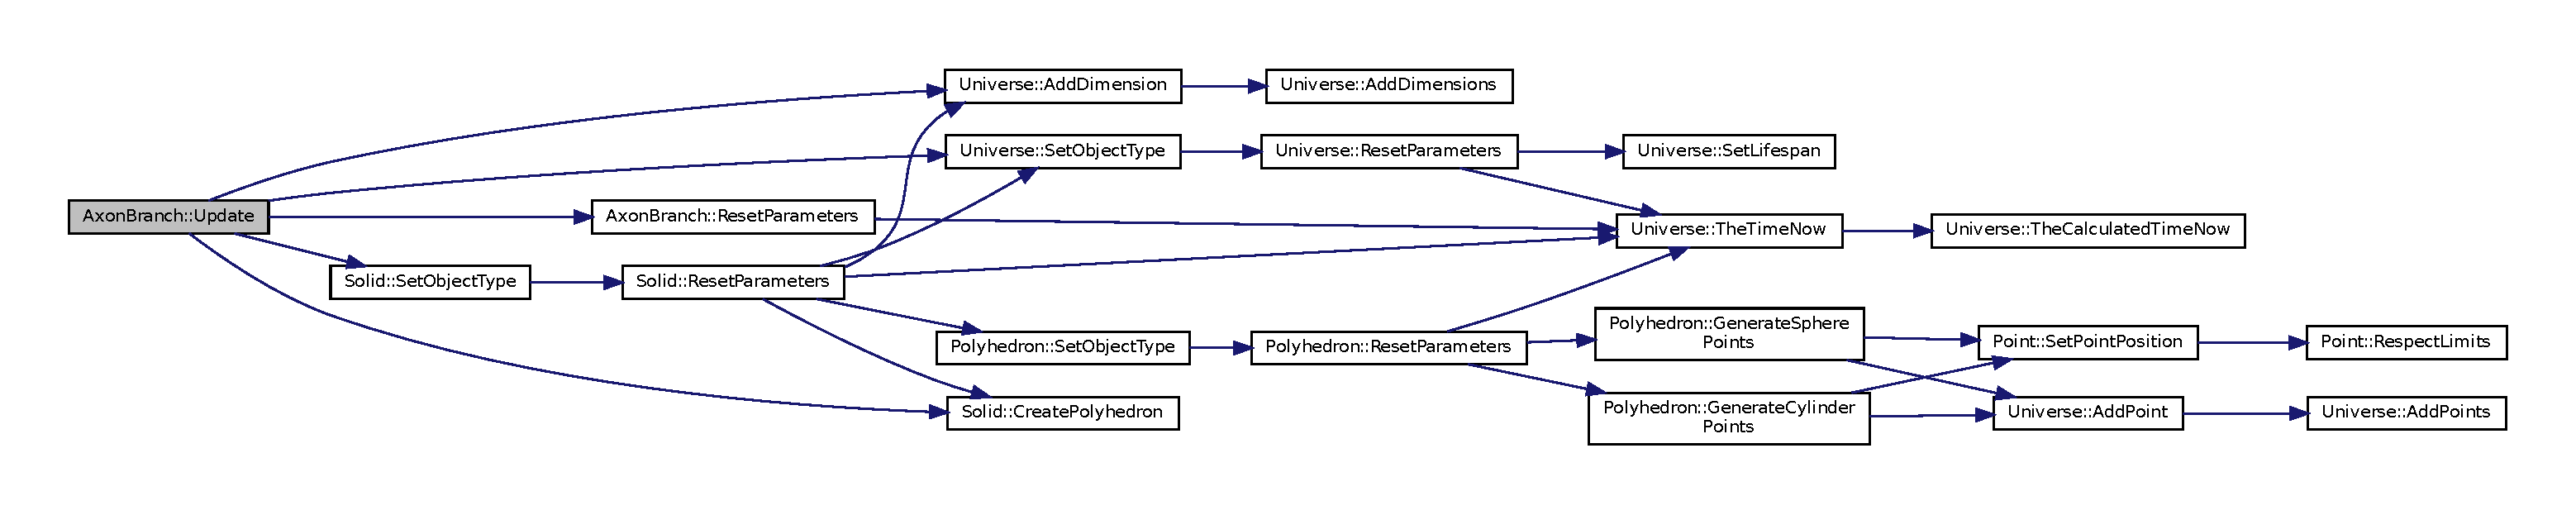
\includegraphics[width=350pt]{class_axon_branch_a5a80bcccdc2be9f77fca25131937b52f_cgraph}
\end{center}
\end{figure}


\subsection{Member Data Documentation}
\mbox{\Hypertarget{class_axon_branch_a43224f9fcb62274709438c9833cb10e5}\label{class_axon_branch_a43224f9fcb62274709438c9833cb10e5}} 
\index{Axon\+Branch@{Axon\+Branch}!axonbouton\+\_\+list@{axonbouton\+\_\+list}}
\index{axonbouton\+\_\+list@{axonbouton\+\_\+list}!Axon\+Branch@{Axon\+Branch}}
\subsubsection{\texorpdfstring{axonbouton\+\_\+list}{axonbouton\_list}}
{\footnotesize\ttfamily std\+::vector$<$\mbox{\hyperlink{class_axon_branch}{Axon\+Branch}}$\ast$$>$ Axon\+Branch\+::axonbouton\+\_\+list\hspace{0.3cm}{\ttfamily [protected]}}



Definition at line 72 of file axonbranch.\+h.



The documentation for this class was generated from the following files\+:\begin{DoxyCompactItemize}
\item 
Brain\+Harmonics/\mbox{\hyperlink{axonbranch_8h}{axonbranch.\+h}}\item 
Brain\+Harmonics/\mbox{\hyperlink{axonbranch_8cc}{axonbranch.\+cc}}\end{DoxyCompactItemize}

\hypertarget{class_axon_hillock}{}\section{Axon\+Hillock Class Reference}
\label{class_axon_hillock}\index{Axon\+Hillock@{Axon\+Hillock}}


{\ttfamily \#include $<$axonhillock.\+h$>$}



Inheritance diagram for Axon\+Hillock\+:\nopagebreak
\begin{figure}[H]
\begin{center}
\leavevmode
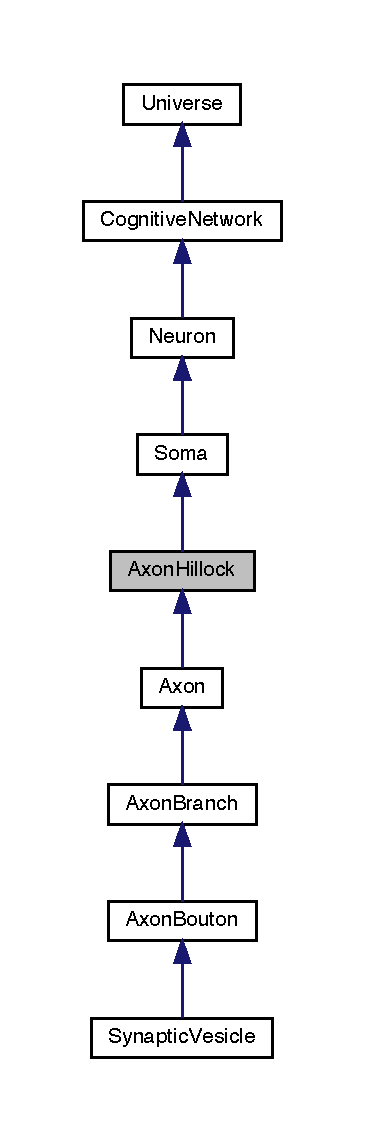
\includegraphics[width=175pt]{class_axon_hillock__inherit__graph}
\end{center}
\end{figure}


Collaboration diagram for Axon\+Hillock\+:
\nopagebreak
\begin{figure}[H]
\begin{center}
\leavevmode
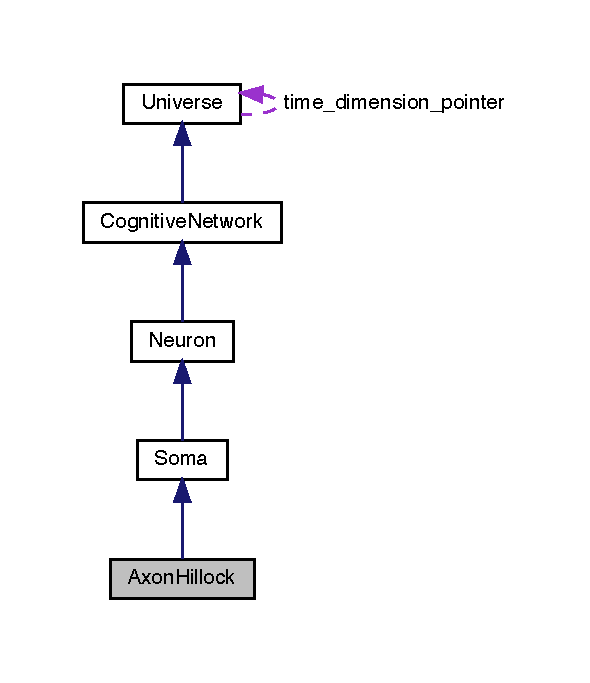
\includegraphics[width=283pt]{class_axon_hillock__coll__graph}
\end{center}
\end{figure}
\subsection*{Public Member Functions}
\begin{DoxyCompactItemize}
\item 
\hyperlink{class_axon_hillock_a432095dfb25ece393cdd83b5eb4f097a}{Axon\+Hillock} ()
\item 
\hyperlink{class_axon_hillock_a20a4da0885f32bfca34ab5cda2a13562}{Axon\+Hillock} (unsigned int object\+\_\+type)
\item 
\hyperlink{class_axon_hillock_acc61c61c8dfddd603e868a2fcbfd5e9c}{Axon\+Hillock} (unsigned int object\+\_\+type, std\+::chrono\+::time\+\_\+point$<$ \hyperlink{universe_8h_a0ef8d951d1ca5ab3cfaf7ab4c7a6fd80}{Clock} $>$ event\+\_\+time)
\item 
\hyperlink{class_axon_hillock_a250945e24a51475369b6c7881c0d955b}{Axon\+Hillock} (unsigned int object\+\_\+type, std\+::chrono\+::time\+\_\+point$<$ \hyperlink{universe_8h_a0ef8d951d1ca5ab3cfaf7ab4c7a6fd80}{Clock} $>$ event\+\_\+time, \hyperlink{class_soma}{Soma} \&soma\+\_\+connector)
\item 
virtual \hyperlink{class_axon_hillock_ae86220026d7c87edc1c514521d66f992}{$\sim$\+Axon\+Hillock} ()
\item 
unsigned int \hyperlink{class_axon_hillock_a429c9876d679fe8de4533725afc4875c}{Get\+Counter} (std\+::chrono\+::time\+\_\+point$<$ \hyperlink{universe_8h_a0ef8d951d1ca5ab3cfaf7ab4c7a6fd80}{Clock} $>$ event\+\_\+time)
\item 
double \hyperlink{class_axon_hillock_ab5ac3ab8771b96acf7e3fa07152525a5}{Get\+Energy} (std\+::chrono\+::time\+\_\+point$<$ \hyperlink{universe_8h_a0ef8d951d1ca5ab3cfaf7ab4c7a6fd80}{Clock} $>$ event\+\_\+time)
\item 
void \hyperlink{class_axon_hillock_a0220cee0ad99ddc48496982078c1856c}{Set\+Counter} (std\+::chrono\+::time\+\_\+point$<$ \hyperlink{universe_8h_a0ef8d951d1ca5ab3cfaf7ab4c7a6fd80}{Clock} $>$ event\+\_\+time, unsigned int val)
\item 
void \hyperlink{class_axon_hillock_a830afd18810e0eaa11a9e7a500b8f0c4}{Set\+Energy} (std\+::chrono\+::time\+\_\+point$<$ \hyperlink{universe_8h_a0ef8d951d1ca5ab3cfaf7ab4c7a6fd80}{Clock} $>$ event\+\_\+time, double val)
\item 
bool \hyperlink{class_axon_hillock_acec1571ef0b74f7f5ce6699c9b459b4f}{Reset\+Parameters} (std\+::chrono\+::time\+\_\+point$<$ \hyperlink{universe_8h_a0ef8d951d1ca5ab3cfaf7ab4c7a6fd80}{Clock} $>$ event\+\_\+time)
\item 
\hyperlink{class_axon_hillock}{Axon\+Hillock} $\ast$ \hyperlink{class_axon_hillock_ae6b18ec6f2921b9d4461b89a9d72ab25}{Create\+Axon} (std\+::chrono\+::time\+\_\+point$<$ \hyperlink{universe_8h_a0ef8d951d1ca5ab3cfaf7ab4c7a6fd80}{Clock} $>$ event\+\_\+time)
\item 
std\+::vector$<$ \hyperlink{class_axon_hillock}{Axon\+Hillock} $\ast$ $>$ \hyperlink{class_axon_hillock_a15bf1a433f38b8b0c92e4a4efe22ec6f}{Create\+Axons} (std\+::chrono\+::time\+\_\+point$<$ \hyperlink{universe_8h_a0ef8d951d1ca5ab3cfaf7ab4c7a6fd80}{Clock} $>$ event\+\_\+time, int quantity)
\item 
\hyperlink{class_axon_hillock}{Axon\+Hillock} $\ast$ \hyperlink{class_axon_hillock_ad54833cee03cfcacb5e88d174048aaa4}{Clone\+Axon} (std\+::chrono\+::time\+\_\+point$<$ \hyperlink{universe_8h_a0ef8d951d1ca5ab3cfaf7ab4c7a6fd80}{Clock} $>$ event\+\_\+time, \hyperlink{class_axon_hillock}{Axon\+Hillock} $\ast$clone\+\_\+object, double perfection\+\_\+membership)
\item 
std\+::vector$<$ \hyperlink{class_axon_hillock}{Axon\+Hillock} $\ast$ $>$ \hyperlink{class_axon_hillock_aa65cead56b10bda66dc256c68764a553}{Clone\+Axons} (std\+::chrono\+::time\+\_\+point$<$ \hyperlink{universe_8h_a0ef8d951d1ca5ab3cfaf7ab4c7a6fd80}{Clock} $>$ event\+\_\+time, std\+::vector$<$ \hyperlink{class_axon_hillock}{Axon\+Hillock} $\ast$$>$ cloning\+\_\+list, double perfection\+\_\+membership)
\item 
\hyperlink{class_axon_hillock}{Axon\+Hillock} $\ast$ \hyperlink{class_axon_hillock_a031b2cc7292d023506a5124639a941a7}{Destroy\+Axon} (std\+::chrono\+::time\+\_\+point$<$ \hyperlink{universe_8h_a0ef8d951d1ca5ab3cfaf7ab4c7a6fd80}{Clock} $>$ event\+\_\+time, \hyperlink{class_axon_hillock}{Axon\+Hillock} $\ast$destroy\+\_\+object)
\item 
std\+::vector$<$ \hyperlink{class_axon_hillock}{Axon\+Hillock} $\ast$ $>$ \hyperlink{class_axon_hillock_a083c918c64c60f3cea1d39aa8e0c6fba}{Destroy\+Axons} (std\+::chrono\+::time\+\_\+point$<$ \hyperlink{universe_8h_a0ef8d951d1ca5ab3cfaf7ab4c7a6fd80}{Clock} $>$ event\+\_\+time, std\+::vector$<$ \hyperlink{class_axon_hillock}{Axon\+Hillock} $\ast$$>$ destruction\+\_\+list)
\item 
\hyperlink{class_axon_hillock}{Axon\+Hillock} $\ast$ \hyperlink{class_axon_hillock_a02bfbaea9ea7a160933f8500c8b41d6a}{Add\+Axon} (std\+::chrono\+::time\+\_\+point$<$ \hyperlink{universe_8h_a0ef8d951d1ca5ab3cfaf7ab4c7a6fd80}{Clock} $>$ event\+\_\+time, \hyperlink{class_axon_hillock}{Axon\+Hillock} $\ast$add\+\_\+object)
\item 
std\+::vector$<$ \hyperlink{class_axon_hillock}{Axon\+Hillock} $\ast$ $>$ \hyperlink{class_axon_hillock_a54a82227b96757f1c0d7450df6a3df37}{Add\+Axons} (std\+::chrono\+::time\+\_\+point$<$ \hyperlink{universe_8h_a0ef8d951d1ca5ab3cfaf7ab4c7a6fd80}{Clock} $>$ event\+\_\+time, std\+::vector$<$ \hyperlink{class_axon_hillock}{Axon\+Hillock} $\ast$$>$ add\+\_\+objects)
\item 
\hyperlink{class_axon_hillock}{Axon\+Hillock} $\ast$ \hyperlink{class_axon_hillock_ae7c379ef3a70c8a43a0f105ccc94b54b}{Remove\+Axon} (std\+::chrono\+::time\+\_\+point$<$ \hyperlink{universe_8h_a0ef8d951d1ca5ab3cfaf7ab4c7a6fd80}{Clock} $>$ event\+\_\+time)
\item 
std\+::vector$<$ \hyperlink{class_axon_hillock}{Axon\+Hillock} $\ast$ $>$ \hyperlink{class_axon_hillock_a7f10edff727271408887d29a70e7e671}{Remove\+Axons} (std\+::chrono\+::time\+\_\+point$<$ \hyperlink{universe_8h_a0ef8d951d1ca5ab3cfaf7ab4c7a6fd80}{Clock} $>$ event\+\_\+time, int quantity)
\item 
\hyperlink{class_axon_hillock}{Axon\+Hillock} $\ast$ \hyperlink{class_axon_hillock_a08fde7d1b8a40ba7a052315f95b743f0}{Get\+Axon} (std\+::chrono\+::time\+\_\+point$<$ \hyperlink{universe_8h_a0ef8d951d1ca5ab3cfaf7ab4c7a6fd80}{Clock} $>$ event\+\_\+time, int selector)
\item 
std\+::vector$<$ \hyperlink{class_axon_hillock}{Axon\+Hillock} $\ast$ $>$ \hyperlink{class_axon_hillock_af35663768cbe818e092382519a6d73e3}{Get\+Axons} (std\+::chrono\+::time\+\_\+point$<$ \hyperlink{universe_8h_a0ef8d951d1ca5ab3cfaf7ab4c7a6fd80}{Clock} $>$ event\+\_\+time)
\item 
int \hyperlink{class_axon_hillock_a5c5cd9008f1410898980528b959d668e}{Growth} (std\+::chrono\+::time\+\_\+point$<$ \hyperlink{universe_8h_a0ef8d951d1ca5ab3cfaf7ab4c7a6fd80}{Clock} $>$ event\+\_\+time)
\item 
int \hyperlink{class_axon_hillock_a5a6a6a93a98b32c303b9ee6320c09909}{Update} (std\+::chrono\+::time\+\_\+point$<$ \hyperlink{universe_8h_a0ef8d951d1ca5ab3cfaf7ab4c7a6fd80}{Clock} $>$ event\+\_\+time)
\end{DoxyCompactItemize}
\subsection*{Protected Attributes}
\begin{DoxyCompactItemize}
\item 
std\+::vector$<$ \hyperlink{class_axon_hillock}{Axon\+Hillock} $\ast$ $>$ \hyperlink{class_axon_hillock_a110d655ded8e09306b224b6e940cd60b}{axon\+\_\+list}
\end{DoxyCompactItemize}
\subsection*{Additional Inherited Members}


\subsection{Detailed Description}


Definition at line 15 of file axonhillock.\+h.



\subsection{Constructor \& Destructor Documentation}
\mbox{\Hypertarget{class_axon_hillock_a432095dfb25ece393cdd83b5eb4f097a}\label{class_axon_hillock_a432095dfb25ece393cdd83b5eb4f097a}} 
\index{Axon\+Hillock@{Axon\+Hillock}!Axon\+Hillock@{Axon\+Hillock}}
\index{Axon\+Hillock@{Axon\+Hillock}!Axon\+Hillock@{Axon\+Hillock}}
\subsubsection{\texorpdfstring{Axon\+Hillock()}{AxonHillock()}\hspace{0.1cm}{\footnotesize\ttfamily [1/4]}}
{\footnotesize\ttfamily Axon\+Hillock\+::\+Axon\+Hillock (\begin{DoxyParamCaption}{ }\end{DoxyParamCaption})\hspace{0.3cm}{\ttfamily [inline]}}



Definition at line 18 of file axonhillock.\+h.

\mbox{\Hypertarget{class_axon_hillock_a20a4da0885f32bfca34ab5cda2a13562}\label{class_axon_hillock_a20a4da0885f32bfca34ab5cda2a13562}} 
\index{Axon\+Hillock@{Axon\+Hillock}!Axon\+Hillock@{Axon\+Hillock}}
\index{Axon\+Hillock@{Axon\+Hillock}!Axon\+Hillock@{Axon\+Hillock}}
\subsubsection{\texorpdfstring{Axon\+Hillock()}{AxonHillock()}\hspace{0.1cm}{\footnotesize\ttfamily [2/4]}}
{\footnotesize\ttfamily Axon\+Hillock\+::\+Axon\+Hillock (\begin{DoxyParamCaption}\item[{unsigned int}]{object\+\_\+type }\end{DoxyParamCaption})\hspace{0.3cm}{\ttfamily [inline]}}



Definition at line 20 of file axonhillock.\+h.

\mbox{\Hypertarget{class_axon_hillock_acc61c61c8dfddd603e868a2fcbfd5e9c}\label{class_axon_hillock_acc61c61c8dfddd603e868a2fcbfd5e9c}} 
\index{Axon\+Hillock@{Axon\+Hillock}!Axon\+Hillock@{Axon\+Hillock}}
\index{Axon\+Hillock@{Axon\+Hillock}!Axon\+Hillock@{Axon\+Hillock}}
\subsubsection{\texorpdfstring{Axon\+Hillock()}{AxonHillock()}\hspace{0.1cm}{\footnotesize\ttfamily [3/4]}}
{\footnotesize\ttfamily Axon\+Hillock\+::\+Axon\+Hillock (\begin{DoxyParamCaption}\item[{unsigned int}]{object\+\_\+type,  }\item[{std\+::chrono\+::time\+\_\+point$<$ \hyperlink{universe_8h_a0ef8d951d1ca5ab3cfaf7ab4c7a6fd80}{Clock} $>$}]{event\+\_\+time }\end{DoxyParamCaption})\hspace{0.3cm}{\ttfamily [inline]}}



Definition at line 22 of file axonhillock.\+h.

\mbox{\Hypertarget{class_axon_hillock_a250945e24a51475369b6c7881c0d955b}\label{class_axon_hillock_a250945e24a51475369b6c7881c0d955b}} 
\index{Axon\+Hillock@{Axon\+Hillock}!Axon\+Hillock@{Axon\+Hillock}}
\index{Axon\+Hillock@{Axon\+Hillock}!Axon\+Hillock@{Axon\+Hillock}}
\subsubsection{\texorpdfstring{Axon\+Hillock()}{AxonHillock()}\hspace{0.1cm}{\footnotesize\ttfamily [4/4]}}
{\footnotesize\ttfamily Axon\+Hillock\+::\+Axon\+Hillock (\begin{DoxyParamCaption}\item[{unsigned int}]{object\+\_\+type,  }\item[{std\+::chrono\+::time\+\_\+point$<$ \hyperlink{universe_8h_a0ef8d951d1ca5ab3cfaf7ab4c7a6fd80}{Clock} $>$}]{event\+\_\+time,  }\item[{\hyperlink{class_soma}{Soma} \&}]{soma\+\_\+connector }\end{DoxyParamCaption})\hspace{0.3cm}{\ttfamily [inline]}}



Definition at line 24 of file axonhillock.\+h.

Here is the call graph for this function\+:
\nopagebreak
\begin{figure}[H]
\begin{center}
\leavevmode
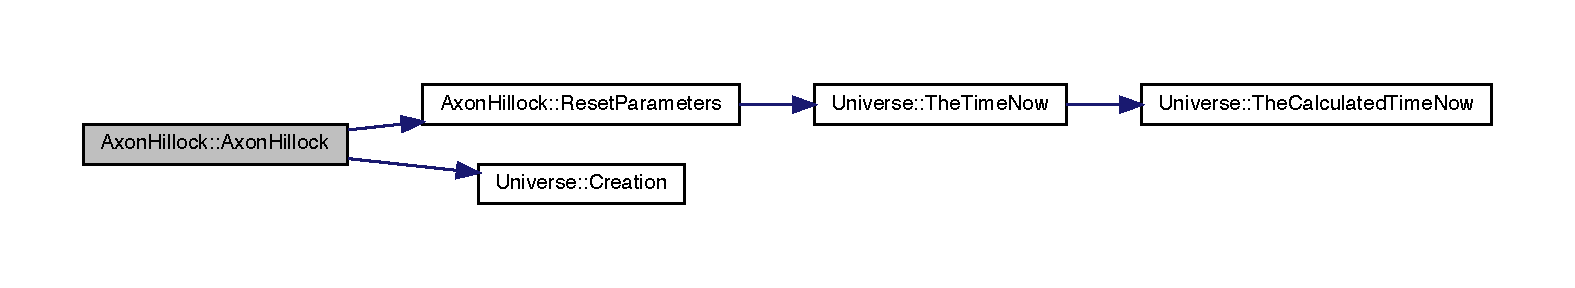
\includegraphics[width=350pt]{class_axon_hillock_a250945e24a51475369b6c7881c0d955b_cgraph}
\end{center}
\end{figure}
\mbox{\Hypertarget{class_axon_hillock_ae86220026d7c87edc1c514521d66f992}\label{class_axon_hillock_ae86220026d7c87edc1c514521d66f992}} 
\index{Axon\+Hillock@{Axon\+Hillock}!````~Axon\+Hillock@{$\sim$\+Axon\+Hillock}}
\index{````~Axon\+Hillock@{$\sim$\+Axon\+Hillock}!Axon\+Hillock@{Axon\+Hillock}}
\subsubsection{\texorpdfstring{$\sim$\+Axon\+Hillock()}{~AxonHillock()}}
{\footnotesize\ttfamily virtual Axon\+Hillock\+::$\sim$\+Axon\+Hillock (\begin{DoxyParamCaption}{ }\end{DoxyParamCaption})\hspace{0.3cm}{\ttfamily [inline]}, {\ttfamily [virtual]}}

Default destructor 

Definition at line 37 of file axonhillock.\+h.



\subsection{Member Function Documentation}
\mbox{\Hypertarget{class_axon_hillock_a02bfbaea9ea7a160933f8500c8b41d6a}\label{class_axon_hillock_a02bfbaea9ea7a160933f8500c8b41d6a}} 
\index{Axon\+Hillock@{Axon\+Hillock}!Add\+Axon@{Add\+Axon}}
\index{Add\+Axon@{Add\+Axon}!Axon\+Hillock@{Axon\+Hillock}}
\subsubsection{\texorpdfstring{Add\+Axon()}{AddAxon()}}
{\footnotesize\ttfamily \hyperlink{class_axon_hillock}{Axon\+Hillock} $\ast$ Axon\+Hillock\+::\+Add\+Axon (\begin{DoxyParamCaption}\item[{std\+::chrono\+::time\+\_\+point$<$ \hyperlink{universe_8h_a0ef8d951d1ca5ab3cfaf7ab4c7a6fd80}{Clock} $>$}]{event\+\_\+time,  }\item[{\hyperlink{class_axon_hillock}{Axon\+Hillock} $\ast$}]{add\+\_\+object }\end{DoxyParamCaption})}



Definition at line 121 of file axonhillock.\+cc.

Here is the caller graph for this function\+:\nopagebreak
\begin{figure}[H]
\begin{center}
\leavevmode
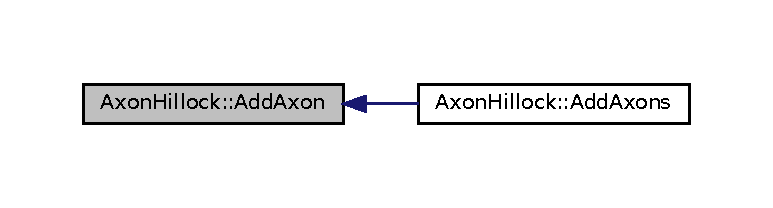
\includegraphics[width=350pt]{class_axon_hillock_a02bfbaea9ea7a160933f8500c8b41d6a_icgraph}
\end{center}
\end{figure}
\mbox{\Hypertarget{class_axon_hillock_a54a82227b96757f1c0d7450df6a3df37}\label{class_axon_hillock_a54a82227b96757f1c0d7450df6a3df37}} 
\index{Axon\+Hillock@{Axon\+Hillock}!Add\+Axons@{Add\+Axons}}
\index{Add\+Axons@{Add\+Axons}!Axon\+Hillock@{Axon\+Hillock}}
\subsubsection{\texorpdfstring{Add\+Axons()}{AddAxons()}}
{\footnotesize\ttfamily std\+::vector$<$ \hyperlink{class_axon_hillock}{Axon\+Hillock} $\ast$ $>$ Axon\+Hillock\+::\+Add\+Axons (\begin{DoxyParamCaption}\item[{std\+::chrono\+::time\+\_\+point$<$ \hyperlink{universe_8h_a0ef8d951d1ca5ab3cfaf7ab4c7a6fd80}{Clock} $>$}]{event\+\_\+time,  }\item[{std\+::vector$<$ \hyperlink{class_axon_hillock}{Axon\+Hillock} $\ast$$>$}]{add\+\_\+objects }\end{DoxyParamCaption})}



Definition at line 132 of file axonhillock.\+cc.

Here is the call graph for this function\+:\nopagebreak
\begin{figure}[H]
\begin{center}
\leavevmode
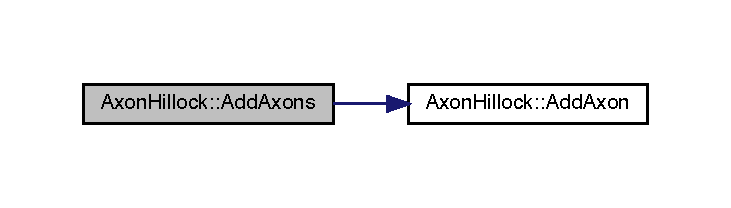
\includegraphics[width=350pt]{class_axon_hillock_a54a82227b96757f1c0d7450df6a3df37_cgraph}
\end{center}
\end{figure}
Here is the caller graph for this function\+:\nopagebreak
\begin{figure}[H]
\begin{center}
\leavevmode
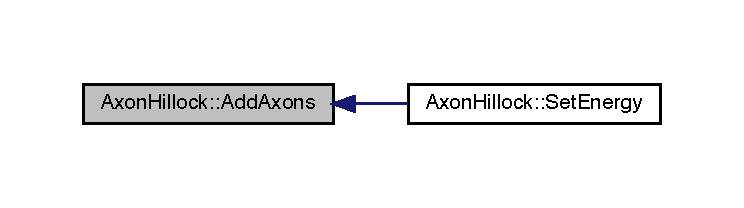
\includegraphics[width=350pt]{class_axon_hillock_a54a82227b96757f1c0d7450df6a3df37_icgraph}
\end{center}
\end{figure}
\mbox{\Hypertarget{class_axon_hillock_ad54833cee03cfcacb5e88d174048aaa4}\label{class_axon_hillock_ad54833cee03cfcacb5e88d174048aaa4}} 
\index{Axon\+Hillock@{Axon\+Hillock}!Clone\+Axon@{Clone\+Axon}}
\index{Clone\+Axon@{Clone\+Axon}!Axon\+Hillock@{Axon\+Hillock}}
\subsubsection{\texorpdfstring{Clone\+Axon()}{CloneAxon()}}
{\footnotesize\ttfamily \hyperlink{class_axon_hillock}{Axon\+Hillock} $\ast$ Axon\+Hillock\+::\+Clone\+Axon (\begin{DoxyParamCaption}\item[{std\+::chrono\+::time\+\_\+point$<$ \hyperlink{universe_8h_a0ef8d951d1ca5ab3cfaf7ab4c7a6fd80}{Clock} $>$}]{event\+\_\+time,  }\item[{\hyperlink{class_axon_hillock}{Axon\+Hillock} $\ast$}]{clone\+\_\+object,  }\item[{double}]{perfection\+\_\+membership }\end{DoxyParamCaption})}



Definition at line 106 of file axonhillock.\+cc.

Here is the caller graph for this function\+:\nopagebreak
\begin{figure}[H]
\begin{center}
\leavevmode
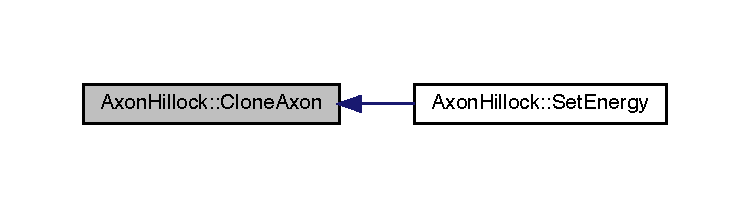
\includegraphics[width=350pt]{class_axon_hillock_ad54833cee03cfcacb5e88d174048aaa4_icgraph}
\end{center}
\end{figure}
\mbox{\Hypertarget{class_axon_hillock_aa65cead56b10bda66dc256c68764a553}\label{class_axon_hillock_aa65cead56b10bda66dc256c68764a553}} 
\index{Axon\+Hillock@{Axon\+Hillock}!Clone\+Axons@{Clone\+Axons}}
\index{Clone\+Axons@{Clone\+Axons}!Axon\+Hillock@{Axon\+Hillock}}
\subsubsection{\texorpdfstring{Clone\+Axons()}{CloneAxons()}}
{\footnotesize\ttfamily std\+::vector$<$ \hyperlink{class_axon_hillock}{Axon\+Hillock} $\ast$ $>$ Axon\+Hillock\+::\+Clone\+Axons (\begin{DoxyParamCaption}\item[{std\+::chrono\+::time\+\_\+point$<$ \hyperlink{universe_8h_a0ef8d951d1ca5ab3cfaf7ab4c7a6fd80}{Clock} $>$}]{event\+\_\+time,  }\item[{std\+::vector$<$ \hyperlink{class_axon_hillock}{Axon\+Hillock} $\ast$$>$}]{cloning\+\_\+list,  }\item[{double}]{perfection\+\_\+membership }\end{DoxyParamCaption})}



Definition at line 101 of file axonhillock.\+cc.

Here is the caller graph for this function\+:\nopagebreak
\begin{figure}[H]
\begin{center}
\leavevmode
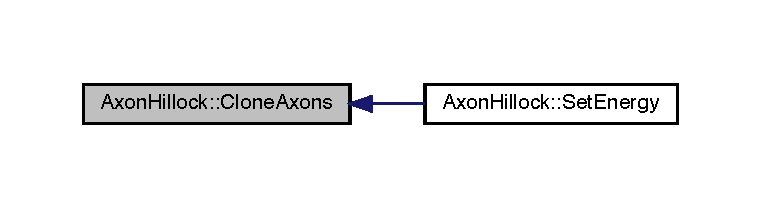
\includegraphics[width=350pt]{class_axon_hillock_aa65cead56b10bda66dc256c68764a553_icgraph}
\end{center}
\end{figure}
\mbox{\Hypertarget{class_axon_hillock_ae6b18ec6f2921b9d4461b89a9d72ab25}\label{class_axon_hillock_ae6b18ec6f2921b9d4461b89a9d72ab25}} 
\index{Axon\+Hillock@{Axon\+Hillock}!Create\+Axon@{Create\+Axon}}
\index{Create\+Axon@{Create\+Axon}!Axon\+Hillock@{Axon\+Hillock}}
\subsubsection{\texorpdfstring{Create\+Axon()}{CreateAxon()}}
{\footnotesize\ttfamily \hyperlink{class_axon_hillock}{Axon\+Hillock} $\ast$ Axon\+Hillock\+::\+Create\+Axon (\begin{DoxyParamCaption}\item[{std\+::chrono\+::time\+\_\+point$<$ \hyperlink{universe_8h_a0ef8d951d1ca5ab3cfaf7ab4c7a6fd80}{Clock} $>$}]{event\+\_\+time }\end{DoxyParamCaption})}



Definition at line 68 of file axonhillock.\+cc.

Here is the caller graph for this function\+:
\nopagebreak
\begin{figure}[H]
\begin{center}
\leavevmode
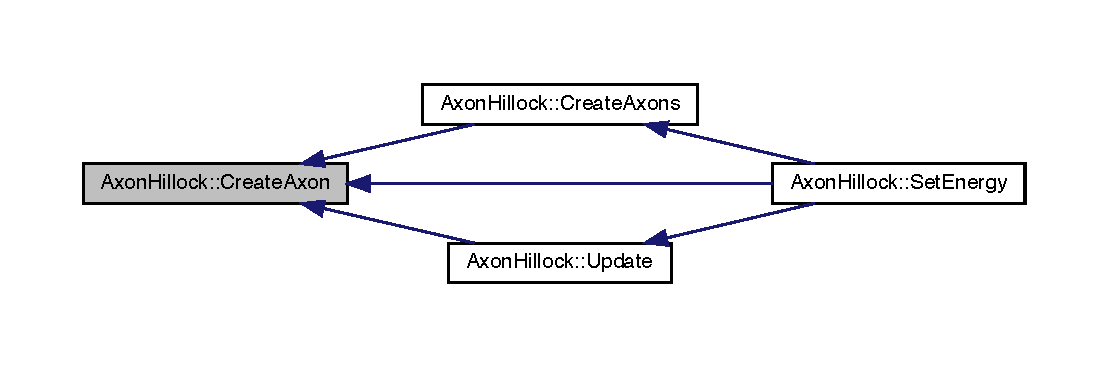
\includegraphics[width=350pt]{class_axon_hillock_ae6b18ec6f2921b9d4461b89a9d72ab25_icgraph}
\end{center}
\end{figure}
\mbox{\Hypertarget{class_axon_hillock_a15bf1a433f38b8b0c92e4a4efe22ec6f}\label{class_axon_hillock_a15bf1a433f38b8b0c92e4a4efe22ec6f}} 
\index{Axon\+Hillock@{Axon\+Hillock}!Create\+Axons@{Create\+Axons}}
\index{Create\+Axons@{Create\+Axons}!Axon\+Hillock@{Axon\+Hillock}}
\subsubsection{\texorpdfstring{Create\+Axons()}{CreateAxons()}}
{\footnotesize\ttfamily std\+::vector$<$ \hyperlink{class_axon_hillock}{Axon\+Hillock} $\ast$ $>$ Axon\+Hillock\+::\+Create\+Axons (\begin{DoxyParamCaption}\item[{std\+::chrono\+::time\+\_\+point$<$ \hyperlink{universe_8h_a0ef8d951d1ca5ab3cfaf7ab4c7a6fd80}{Clock} $>$}]{event\+\_\+time,  }\item[{int}]{quantity }\end{DoxyParamCaption})}



Definition at line 79 of file axonhillock.\+cc.

Here is the call graph for this function\+:
\nopagebreak
\begin{figure}[H]
\begin{center}
\leavevmode
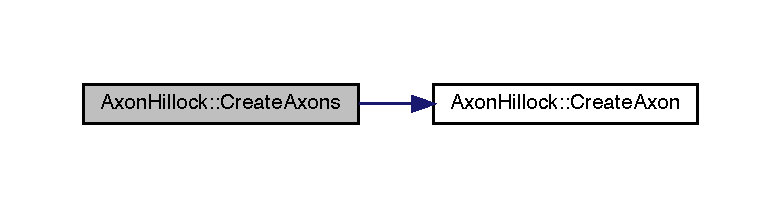
\includegraphics[width=350pt]{class_axon_hillock_a15bf1a433f38b8b0c92e4a4efe22ec6f_cgraph}
\end{center}
\end{figure}
Here is the caller graph for this function\+:
\nopagebreak
\begin{figure}[H]
\begin{center}
\leavevmode
\includegraphics[width=350pt]{class_axon_hillock_a15bf1a433f38b8b0c92e4a4efe22ec6f_icgraph}
\end{center}
\end{figure}
\mbox{\Hypertarget{class_axon_hillock_a031b2cc7292d023506a5124639a941a7}\label{class_axon_hillock_a031b2cc7292d023506a5124639a941a7}} 
\index{Axon\+Hillock@{Axon\+Hillock}!Destroy\+Axon@{Destroy\+Axon}}
\index{Destroy\+Axon@{Destroy\+Axon}!Axon\+Hillock@{Axon\+Hillock}}
\subsubsection{\texorpdfstring{Destroy\+Axon()}{DestroyAxon()}}
{\footnotesize\ttfamily \hyperlink{class_axon_hillock}{Axon\+Hillock} $\ast$ Axon\+Hillock\+::\+Destroy\+Axon (\begin{DoxyParamCaption}\item[{std\+::chrono\+::time\+\_\+point$<$ \hyperlink{universe_8h_a0ef8d951d1ca5ab3cfaf7ab4c7a6fd80}{Clock} $>$}]{event\+\_\+time,  }\item[{\hyperlink{class_axon_hillock}{Axon\+Hillock} $\ast$}]{destroy\+\_\+object }\end{DoxyParamCaption})}



Definition at line 116 of file axonhillock.\+cc.

Here is the caller graph for this function\+:
\nopagebreak
\begin{figure}[H]
\begin{center}
\leavevmode
\includegraphics[width=350pt]{class_axon_hillock_a031b2cc7292d023506a5124639a941a7_icgraph}
\end{center}
\end{figure}
\mbox{\Hypertarget{class_axon_hillock_a083c918c64c60f3cea1d39aa8e0c6fba}\label{class_axon_hillock_a083c918c64c60f3cea1d39aa8e0c6fba}} 
\index{Axon\+Hillock@{Axon\+Hillock}!Destroy\+Axons@{Destroy\+Axons}}
\index{Destroy\+Axons@{Destroy\+Axons}!Axon\+Hillock@{Axon\+Hillock}}
\subsubsection{\texorpdfstring{Destroy\+Axons()}{DestroyAxons()}}
{\footnotesize\ttfamily std\+::vector$<$ \hyperlink{class_axon_hillock}{Axon\+Hillock} $\ast$ $>$ Axon\+Hillock\+::\+Destroy\+Axons (\begin{DoxyParamCaption}\item[{std\+::chrono\+::time\+\_\+point$<$ \hyperlink{universe_8h_a0ef8d951d1ca5ab3cfaf7ab4c7a6fd80}{Clock} $>$}]{event\+\_\+time,  }\item[{std\+::vector$<$ \hyperlink{class_axon_hillock}{Axon\+Hillock} $\ast$$>$}]{destruction\+\_\+list }\end{DoxyParamCaption})}



Definition at line 111 of file axonhillock.\+cc.

Here is the caller graph for this function\+:
\nopagebreak
\begin{figure}[H]
\begin{center}
\leavevmode
\includegraphics[width=350pt]{class_axon_hillock_a083c918c64c60f3cea1d39aa8e0c6fba_icgraph}
\end{center}
\end{figure}
\mbox{\Hypertarget{class_axon_hillock_a08fde7d1b8a40ba7a052315f95b743f0}\label{class_axon_hillock_a08fde7d1b8a40ba7a052315f95b743f0}} 
\index{Axon\+Hillock@{Axon\+Hillock}!Get\+Axon@{Get\+Axon}}
\index{Get\+Axon@{Get\+Axon}!Axon\+Hillock@{Axon\+Hillock}}
\subsubsection{\texorpdfstring{Get\+Axon()}{GetAxon()}}
{\footnotesize\ttfamily \hyperlink{class_axon_hillock}{Axon\+Hillock} $\ast$ Axon\+Hillock\+::\+Get\+Axon (\begin{DoxyParamCaption}\item[{std\+::chrono\+::time\+\_\+point$<$ \hyperlink{universe_8h_a0ef8d951d1ca5ab3cfaf7ab4c7a6fd80}{Clock} $>$}]{event\+\_\+time,  }\item[{int}]{selector }\end{DoxyParamCaption})}



Definition at line 165 of file axonhillock.\+cc.

Here is the caller graph for this function\+:
\nopagebreak
\begin{figure}[H]
\begin{center}
\leavevmode
\includegraphics[width=350pt]{class_axon_hillock_a08fde7d1b8a40ba7a052315f95b743f0_icgraph}
\end{center}
\end{figure}
\mbox{\Hypertarget{class_axon_hillock_af35663768cbe818e092382519a6d73e3}\label{class_axon_hillock_af35663768cbe818e092382519a6d73e3}} 
\index{Axon\+Hillock@{Axon\+Hillock}!Get\+Axons@{Get\+Axons}}
\index{Get\+Axons@{Get\+Axons}!Axon\+Hillock@{Axon\+Hillock}}
\subsubsection{\texorpdfstring{Get\+Axons()}{GetAxons()}}
{\footnotesize\ttfamily std\+::vector$<$ \hyperlink{class_axon_hillock}{Axon\+Hillock} $\ast$ $>$ Axon\+Hillock\+::\+Get\+Axons (\begin{DoxyParamCaption}\item[{std\+::chrono\+::time\+\_\+point$<$ \hyperlink{universe_8h_a0ef8d951d1ca5ab3cfaf7ab4c7a6fd80}{Clock} $>$}]{event\+\_\+time }\end{DoxyParamCaption})}



Definition at line 170 of file axonhillock.\+cc.

Here is the caller graph for this function\+:
\nopagebreak
\begin{figure}[H]
\begin{center}
\leavevmode
\includegraphics[width=350pt]{class_axon_hillock_af35663768cbe818e092382519a6d73e3_icgraph}
\end{center}
\end{figure}
\mbox{\Hypertarget{class_axon_hillock_a429c9876d679fe8de4533725afc4875c}\label{class_axon_hillock_a429c9876d679fe8de4533725afc4875c}} 
\index{Axon\+Hillock@{Axon\+Hillock}!Get\+Counter@{Get\+Counter}}
\index{Get\+Counter@{Get\+Counter}!Axon\+Hillock@{Axon\+Hillock}}
\subsubsection{\texorpdfstring{Get\+Counter()}{GetCounter()}}
{\footnotesize\ttfamily unsigned int Axon\+Hillock\+::\+Get\+Counter (\begin{DoxyParamCaption}\item[{std\+::chrono\+::time\+\_\+point$<$ \hyperlink{universe_8h_a0ef8d951d1ca5ab3cfaf7ab4c7a6fd80}{Clock} $>$}]{event\+\_\+time }\end{DoxyParamCaption})\hspace{0.3cm}{\ttfamily [inline]}}



Definition at line 39 of file axonhillock.\+h.

\mbox{\Hypertarget{class_axon_hillock_ab5ac3ab8771b96acf7e3fa07152525a5}\label{class_axon_hillock_ab5ac3ab8771b96acf7e3fa07152525a5}} 
\index{Axon\+Hillock@{Axon\+Hillock}!Get\+Energy@{Get\+Energy}}
\index{Get\+Energy@{Get\+Energy}!Axon\+Hillock@{Axon\+Hillock}}
\subsubsection{\texorpdfstring{Get\+Energy()}{GetEnergy()}}
{\footnotesize\ttfamily double Axon\+Hillock\+::\+Get\+Energy (\begin{DoxyParamCaption}\item[{std\+::chrono\+::time\+\_\+point$<$ \hyperlink{universe_8h_a0ef8d951d1ca5ab3cfaf7ab4c7a6fd80}{Clock} $>$}]{event\+\_\+time }\end{DoxyParamCaption})\hspace{0.3cm}{\ttfamily [inline]}}



Definition at line 40 of file axonhillock.\+h.

\mbox{\Hypertarget{class_axon_hillock_a5c5cd9008f1410898980528b959d668e}\label{class_axon_hillock_a5c5cd9008f1410898980528b959d668e}} 
\index{Axon\+Hillock@{Axon\+Hillock}!Growth@{Growth}}
\index{Growth@{Growth}!Axon\+Hillock@{Axon\+Hillock}}
\subsubsection{\texorpdfstring{Growth()}{Growth()}}
{\footnotesize\ttfamily int Axon\+Hillock\+::\+Growth (\begin{DoxyParamCaption}\item[{std\+::chrono\+::time\+\_\+point$<$ \hyperlink{universe_8h_a0ef8d951d1ca5ab3cfaf7ab4c7a6fd80}{Clock} $>$}]{event\+\_\+time }\end{DoxyParamCaption})}



Definition at line 176 of file axonhillock.\+cc.

Here is the caller graph for this function\+:\nopagebreak
\begin{figure}[H]
\begin{center}
\leavevmode
\includegraphics[width=350pt]{class_axon_hillock_a5c5cd9008f1410898980528b959d668e_icgraph}
\end{center}
\end{figure}
\mbox{\Hypertarget{class_axon_hillock_ae7c379ef3a70c8a43a0f105ccc94b54b}\label{class_axon_hillock_ae7c379ef3a70c8a43a0f105ccc94b54b}} 
\index{Axon\+Hillock@{Axon\+Hillock}!Remove\+Axon@{Remove\+Axon}}
\index{Remove\+Axon@{Remove\+Axon}!Axon\+Hillock@{Axon\+Hillock}}
\subsubsection{\texorpdfstring{Remove\+Axon()}{RemoveAxon()}}
{\footnotesize\ttfamily \hyperlink{class_axon_hillock}{Axon\+Hillock} $\ast$ Axon\+Hillock\+::\+Remove\+Axon (\begin{DoxyParamCaption}\item[{std\+::chrono\+::time\+\_\+point$<$ \hyperlink{universe_8h_a0ef8d951d1ca5ab3cfaf7ab4c7a6fd80}{Clock} $>$}]{event\+\_\+time }\end{DoxyParamCaption})}



Definition at line 154 of file axonhillock.\+cc.

Here is the caller graph for this function\+:\nopagebreak
\begin{figure}[H]
\begin{center}
\leavevmode
\includegraphics[width=350pt]{class_axon_hillock_ae7c379ef3a70c8a43a0f105ccc94b54b_icgraph}
\end{center}
\end{figure}
\mbox{\Hypertarget{class_axon_hillock_a7f10edff727271408887d29a70e7e671}\label{class_axon_hillock_a7f10edff727271408887d29a70e7e671}} 
\index{Axon\+Hillock@{Axon\+Hillock}!Remove\+Axons@{Remove\+Axons}}
\index{Remove\+Axons@{Remove\+Axons}!Axon\+Hillock@{Axon\+Hillock}}
\subsubsection{\texorpdfstring{Remove\+Axons()}{RemoveAxons()}}
{\footnotesize\ttfamily std\+::vector$<$ \hyperlink{class_axon_hillock}{Axon\+Hillock} $\ast$ $>$ Axon\+Hillock\+::\+Remove\+Axons (\begin{DoxyParamCaption}\item[{std\+::chrono\+::time\+\_\+point$<$ \hyperlink{universe_8h_a0ef8d951d1ca5ab3cfaf7ab4c7a6fd80}{Clock} $>$}]{event\+\_\+time,  }\item[{int}]{quantity }\end{DoxyParamCaption})}



Definition at line 160 of file axonhillock.\+cc.

Here is the caller graph for this function\+:\nopagebreak
\begin{figure}[H]
\begin{center}
\leavevmode
\includegraphics[width=350pt]{class_axon_hillock_a7f10edff727271408887d29a70e7e671_icgraph}
\end{center}
\end{figure}
\mbox{\Hypertarget{class_axon_hillock_acec1571ef0b74f7f5ce6699c9b459b4f}\label{class_axon_hillock_acec1571ef0b74f7f5ce6699c9b459b4f}} 
\index{Axon\+Hillock@{Axon\+Hillock}!Reset\+Parameters@{Reset\+Parameters}}
\index{Reset\+Parameters@{Reset\+Parameters}!Axon\+Hillock@{Axon\+Hillock}}
\subsubsection{\texorpdfstring{Reset\+Parameters()}{ResetParameters()}}
{\footnotesize\ttfamily bool Axon\+Hillock\+::\+Reset\+Parameters (\begin{DoxyParamCaption}\item[{std\+::chrono\+::time\+\_\+point$<$ \hyperlink{universe_8h_a0ef8d951d1ca5ab3cfaf7ab4c7a6fd80}{Clock} $>$}]{event\+\_\+time }\end{DoxyParamCaption})}



Definition at line 20 of file axonhillock.\+cc.

Here is the call graph for this function\+:\nopagebreak
\begin{figure}[H]
\begin{center}
\leavevmode
\includegraphics[width=350pt]{class_axon_hillock_acec1571ef0b74f7f5ce6699c9b459b4f_cgraph}
\end{center}
\end{figure}
Here is the caller graph for this function\+:
\nopagebreak
\begin{figure}[H]
\begin{center}
\leavevmode
\includegraphics[width=350pt]{class_axon_hillock_acec1571ef0b74f7f5ce6699c9b459b4f_icgraph}
\end{center}
\end{figure}
\mbox{\Hypertarget{class_axon_hillock_a0220cee0ad99ddc48496982078c1856c}\label{class_axon_hillock_a0220cee0ad99ddc48496982078c1856c}} 
\index{Axon\+Hillock@{Axon\+Hillock}!Set\+Counter@{Set\+Counter}}
\index{Set\+Counter@{Set\+Counter}!Axon\+Hillock@{Axon\+Hillock}}
\subsubsection{\texorpdfstring{Set\+Counter()}{SetCounter()}}
{\footnotesize\ttfamily void Axon\+Hillock\+::\+Set\+Counter (\begin{DoxyParamCaption}\item[{std\+::chrono\+::time\+\_\+point$<$ \hyperlink{universe_8h_a0ef8d951d1ca5ab3cfaf7ab4c7a6fd80}{Clock} $>$}]{event\+\_\+time,  }\item[{unsigned int}]{val }\end{DoxyParamCaption})\hspace{0.3cm}{\ttfamily [inline]}, {\ttfamily [virtual]}}



Reimplemented from \hyperlink{class_universe_aa22202ae740eb1355529afcb13285e91}{Universe}.



Reimplemented in \hyperlink{class_synaptic_vesicle_a7fd7cfce5eccb904206d968866f85220}{Synaptic\+Vesicle}.



Definition at line 41 of file axonhillock.\+h.

\mbox{\Hypertarget{class_axon_hillock_a830afd18810e0eaa11a9e7a500b8f0c4}\label{class_axon_hillock_a830afd18810e0eaa11a9e7a500b8f0c4}} 
\index{Axon\+Hillock@{Axon\+Hillock}!Set\+Energy@{Set\+Energy}}
\index{Set\+Energy@{Set\+Energy}!Axon\+Hillock@{Axon\+Hillock}}
\subsubsection{\texorpdfstring{Set\+Energy()}{SetEnergy()}}
{\footnotesize\ttfamily void Axon\+Hillock\+::\+Set\+Energy (\begin{DoxyParamCaption}\item[{std\+::chrono\+::time\+\_\+point$<$ \hyperlink{universe_8h_a0ef8d951d1ca5ab3cfaf7ab4c7a6fd80}{Clock} $>$}]{event\+\_\+time,  }\item[{double}]{val }\end{DoxyParamCaption})\hspace{0.3cm}{\ttfamily [inline]}}



Definition at line 42 of file axonhillock.\+h.

Here is the call graph for this function\+:
\nopagebreak
\begin{figure}[H]
\begin{center}
\leavevmode
\includegraphics[width=350pt]{class_axon_hillock_a830afd18810e0eaa11a9e7a500b8f0c4_cgraph}
\end{center}
\end{figure}
\mbox{\Hypertarget{class_axon_hillock_a5a6a6a93a98b32c303b9ee6320c09909}\label{class_axon_hillock_a5a6a6a93a98b32c303b9ee6320c09909}} 
\index{Axon\+Hillock@{Axon\+Hillock}!Update@{Update}}
\index{Update@{Update}!Axon\+Hillock@{Axon\+Hillock}}
\subsubsection{\texorpdfstring{Update()}{Update()}}
{\footnotesize\ttfamily int Axon\+Hillock\+::\+Update (\begin{DoxyParamCaption}\item[{std\+::chrono\+::time\+\_\+point$<$ \hyperlink{universe_8h_a0ef8d951d1ca5ab3cfaf7ab4c7a6fd80}{Clock} $>$}]{event\+\_\+time }\end{DoxyParamCaption})}



Definition at line 197 of file axonhillock.\+cc.

Here is the call graph for this function\+:
\nopagebreak
\begin{figure}[H]
\begin{center}
\leavevmode
\includegraphics[width=350pt]{class_axon_hillock_a5a6a6a93a98b32c303b9ee6320c09909_cgraph}
\end{center}
\end{figure}
Here is the caller graph for this function\+:
\nopagebreak
\begin{figure}[H]
\begin{center}
\leavevmode
\includegraphics[width=344pt]{class_axon_hillock_a5a6a6a93a98b32c303b9ee6320c09909_icgraph}
\end{center}
\end{figure}


\subsection{Member Data Documentation}
\mbox{\Hypertarget{class_axon_hillock_a110d655ded8e09306b224b6e940cd60b}\label{class_axon_hillock_a110d655ded8e09306b224b6e940cd60b}} 
\index{Axon\+Hillock@{Axon\+Hillock}!axon\+\_\+list@{axon\+\_\+list}}
\index{axon\+\_\+list@{axon\+\_\+list}!Axon\+Hillock@{Axon\+Hillock}}
\subsubsection{\texorpdfstring{axon\+\_\+list}{axon\_list}}
{\footnotesize\ttfamily std\+::vector$<$\hyperlink{class_axon_hillock}{Axon\+Hillock}$\ast$$>$ Axon\+Hillock\+::axon\+\_\+list\hspace{0.3cm}{\ttfamily [protected]}}



Definition at line 75 of file axonhillock.\+h.



The documentation for this class was generated from the following files\+:\begin{DoxyCompactItemize}
\item 
Brain\+Harmonics/\hyperlink{axonhillock_8h}{axonhillock.\+h}\item 
Brain\+Harmonics/\hyperlink{axonhillock_8cc}{axonhillock.\+cc}\end{DoxyCompactItemize}

\hypertarget{class_cognitive_input}{}\section{Cognitive\+Input Class Reference}
\label{class_cognitive_input}\index{Cognitive\+Input@{Cognitive\+Input}}


{\ttfamily \#include $<$cognitiveinput.\+h$>$}



Inheritance diagram for Cognitive\+Input\+:\nopagebreak
\begin{figure}[H]
\begin{center}
\leavevmode
\includegraphics[width=175pt]{class_cognitive_input__inherit__graph}
\end{center}
\end{figure}


Collaboration diagram for Cognitive\+Input\+:\nopagebreak
\begin{figure}[H]
\begin{center}
\leavevmode
\includegraphics[width=283pt]{class_cognitive_input__coll__graph}
\end{center}
\end{figure}
\subsection*{Public Member Functions}
\begin{DoxyCompactItemize}
\item 
\mbox{\hyperlink{class_cognitive_input_a5c3c102dc3ec6cfec25eb849488e9782}{Cognitive\+Input}} ()
\item 
\mbox{\hyperlink{class_cognitive_input_a220c07f5be517afe47b4d3c486c4152e}{Cognitive\+Input}} (unsigned int object\+\_\+type)
\item 
\mbox{\hyperlink{class_cognitive_input_a31cc06426ab41c39ec8c795ab29d43de}{Cognitive\+Input}} (unsigned int object\+\_\+type, std\+::chrono\+::time\+\_\+point$<$ \mbox{\hyperlink{universe_8h_a0ef8d951d1ca5ab3cfaf7ab4c7a6fd80}{Clock}} $>$ event\+\_\+time)
\item 
\mbox{\hyperlink{class_cognitive_input_a230ebb8f019af7e0bff51c13bc10c580}{Cognitive\+Input}} (unsigned int object\+\_\+type, std\+::chrono\+::time\+\_\+point$<$ \mbox{\hyperlink{universe_8h_a0ef8d951d1ca5ab3cfaf7ab4c7a6fd80}{Clock}} $>$ event\+\_\+time, \mbox{\hyperlink{class_cognitive_network}{Cognitive\+Network}} \&cognitivenetwork\+\_\+connector)
\item 
virtual \mbox{\hyperlink{class_cognitive_input_a68007661b8fdd7ef39213a1fb3c06bd7}{$\sim$\+Cognitive\+Input}} ()
\item 
unsigned int \mbox{\hyperlink{class_cognitive_input_a695e7e57b717210b64f9e2c4e26c8044}{Get\+Counter}} (std\+::chrono\+::time\+\_\+point$<$ \mbox{\hyperlink{universe_8h_a0ef8d951d1ca5ab3cfaf7ab4c7a6fd80}{Clock}} $>$ event\+\_\+time)
\item 
double \mbox{\hyperlink{class_cognitive_input_a9bdb43198c1a36b97a6da125331bc927}{Get\+Energy}} (std\+::chrono\+::time\+\_\+point$<$ \mbox{\hyperlink{universe_8h_a0ef8d951d1ca5ab3cfaf7ab4c7a6fd80}{Clock}} $>$ event\+\_\+time)
\item 
int \mbox{\hyperlink{class_cognitive_input_a0ad0919c7280b268493b27892bd7c784}{Get\+Type}} (std\+::chrono\+::time\+\_\+point$<$ \mbox{\hyperlink{universe_8h_a0ef8d951d1ca5ab3cfaf7ab4c7a6fd80}{Clock}} $>$ event\+\_\+time)
\item 
\mbox{\hyperlink{glad_8h_a950fc91edb4504f62f1c577bf4727c29}{void}} \mbox{\hyperlink{class_cognitive_input_a37d38512fb190431b4baf8f990c077a9}{Set\+Type}} (std\+::chrono\+::time\+\_\+point$<$ \mbox{\hyperlink{universe_8h_a0ef8d951d1ca5ab3cfaf7ab4c7a6fd80}{Clock}} $>$ event\+\_\+time, int \mbox{\hyperlink{glad_8h_a26942fd2ed566ef553eae82d2c109c8f}{val}})
\item 
\mbox{\hyperlink{glad_8h_a950fc91edb4504f62f1c577bf4727c29}{void}} \mbox{\hyperlink{class_cognitive_input_a4f09c1f176b5406d95a14d7cb1ab75e6}{Set\+Counter}} (std\+::chrono\+::time\+\_\+point$<$ \mbox{\hyperlink{universe_8h_a0ef8d951d1ca5ab3cfaf7ab4c7a6fd80}{Clock}} $>$ event\+\_\+time, unsigned int \mbox{\hyperlink{glad_8h_a26942fd2ed566ef553eae82d2c109c8f}{val}})
\item 
\mbox{\hyperlink{glad_8h_a950fc91edb4504f62f1c577bf4727c29}{void}} \mbox{\hyperlink{class_cognitive_input_a3498a8b5333606ef4d089e6c427ddf74}{Set\+Energy}} (std\+::chrono\+::time\+\_\+point$<$ \mbox{\hyperlink{universe_8h_a0ef8d951d1ca5ab3cfaf7ab4c7a6fd80}{Clock}} $>$ event\+\_\+time, double \mbox{\hyperlink{glad_8h_a26942fd2ed566ef553eae82d2c109c8f}{val}})
\item 
\mbox{\hyperlink{glad_8h_a950fc91edb4504f62f1c577bf4727c29}{void}} \mbox{\hyperlink{class_cognitive_input_a23f56d012233f655e1530ab61d80c27f}{Add\+Energy}} (std\+::chrono\+::time\+\_\+point$<$ \mbox{\hyperlink{universe_8h_a0ef8d951d1ca5ab3cfaf7ab4c7a6fd80}{Clock}} $>$ event\+\_\+time, double \mbox{\hyperlink{glad_8h_a26942fd2ed566ef553eae82d2c109c8f}{val}})
\item 
bool \mbox{\hyperlink{class_cognitive_input_a943605b820cc279533e19d24e11405c6}{Reset\+Parameters}} (std\+::chrono\+::time\+\_\+point$<$ \mbox{\hyperlink{universe_8h_a0ef8d951d1ca5ab3cfaf7ab4c7a6fd80}{Clock}} $>$ event\+\_\+time)
\item 
int \mbox{\hyperlink{class_cognitive_input_a93bd9d88194a545c9a85512edcbb6044}{Update}} (std\+::chrono\+::time\+\_\+point$<$ \mbox{\hyperlink{universe_8h_a0ef8d951d1ca5ab3cfaf7ab4c7a6fd80}{Clock}} $>$ event\+\_\+time)
\end{DoxyCompactItemize}
\subsection*{Additional Inherited Members}


\subsection{Detailed Description}


Definition at line 17 of file cognitiveinput.\+h.



\subsection{Constructor \& Destructor Documentation}
\mbox{\Hypertarget{class_cognitive_input_a5c3c102dc3ec6cfec25eb849488e9782}\label{class_cognitive_input_a5c3c102dc3ec6cfec25eb849488e9782}} 
\index{Cognitive\+Input@{Cognitive\+Input}!Cognitive\+Input@{Cognitive\+Input}}
\index{Cognitive\+Input@{Cognitive\+Input}!Cognitive\+Input@{Cognitive\+Input}}
\subsubsection{\texorpdfstring{Cognitive\+Input()}{CognitiveInput()}\hspace{0.1cm}{\footnotesize\ttfamily [1/4]}}
{\footnotesize\ttfamily Cognitive\+Input\+::\+Cognitive\+Input (\begin{DoxyParamCaption}{ }\end{DoxyParamCaption})\hspace{0.3cm}{\ttfamily [inline]}}



Definition at line 20 of file cognitiveinput.\+h.

\mbox{\Hypertarget{class_cognitive_input_a220c07f5be517afe47b4d3c486c4152e}\label{class_cognitive_input_a220c07f5be517afe47b4d3c486c4152e}} 
\index{Cognitive\+Input@{Cognitive\+Input}!Cognitive\+Input@{Cognitive\+Input}}
\index{Cognitive\+Input@{Cognitive\+Input}!Cognitive\+Input@{Cognitive\+Input}}
\subsubsection{\texorpdfstring{Cognitive\+Input()}{CognitiveInput()}\hspace{0.1cm}{\footnotesize\ttfamily [2/4]}}
{\footnotesize\ttfamily Cognitive\+Input\+::\+Cognitive\+Input (\begin{DoxyParamCaption}\item[{unsigned int}]{object\+\_\+type }\end{DoxyParamCaption})\hspace{0.3cm}{\ttfamily [inline]}}



Definition at line 22 of file cognitiveinput.\+h.

\mbox{\Hypertarget{class_cognitive_input_a31cc06426ab41c39ec8c795ab29d43de}\label{class_cognitive_input_a31cc06426ab41c39ec8c795ab29d43de}} 
\index{Cognitive\+Input@{Cognitive\+Input}!Cognitive\+Input@{Cognitive\+Input}}
\index{Cognitive\+Input@{Cognitive\+Input}!Cognitive\+Input@{Cognitive\+Input}}
\subsubsection{\texorpdfstring{Cognitive\+Input()}{CognitiveInput()}\hspace{0.1cm}{\footnotesize\ttfamily [3/4]}}
{\footnotesize\ttfamily Cognitive\+Input\+::\+Cognitive\+Input (\begin{DoxyParamCaption}\item[{unsigned int}]{object\+\_\+type,  }\item[{std\+::chrono\+::time\+\_\+point$<$ \mbox{\hyperlink{universe_8h_a0ef8d951d1ca5ab3cfaf7ab4c7a6fd80}{Clock}} $>$}]{event\+\_\+time }\end{DoxyParamCaption})\hspace{0.3cm}{\ttfamily [inline]}}



Definition at line 24 of file cognitiveinput.\+h.

\mbox{\Hypertarget{class_cognitive_input_a230ebb8f019af7e0bff51c13bc10c580}\label{class_cognitive_input_a230ebb8f019af7e0bff51c13bc10c580}} 
\index{Cognitive\+Input@{Cognitive\+Input}!Cognitive\+Input@{Cognitive\+Input}}
\index{Cognitive\+Input@{Cognitive\+Input}!Cognitive\+Input@{Cognitive\+Input}}
\subsubsection{\texorpdfstring{Cognitive\+Input()}{CognitiveInput()}\hspace{0.1cm}{\footnotesize\ttfamily [4/4]}}
{\footnotesize\ttfamily Cognitive\+Input\+::\+Cognitive\+Input (\begin{DoxyParamCaption}\item[{unsigned int}]{object\+\_\+type,  }\item[{std\+::chrono\+::time\+\_\+point$<$ \mbox{\hyperlink{universe_8h_a0ef8d951d1ca5ab3cfaf7ab4c7a6fd80}{Clock}} $>$}]{event\+\_\+time,  }\item[{\mbox{\hyperlink{class_cognitive_network}{Cognitive\+Network}} \&}]{cognitivenetwork\+\_\+connector }\end{DoxyParamCaption})\hspace{0.3cm}{\ttfamily [inline]}}



Definition at line 26 of file cognitiveinput.\+h.

Here is the call graph for this function\+:\nopagebreak
\begin{figure}[H]
\begin{center}
\leavevmode
\includegraphics[width=350pt]{class_cognitive_input_a230ebb8f019af7e0bff51c13bc10c580_cgraph}
\end{center}
\end{figure}
\mbox{\Hypertarget{class_cognitive_input_a68007661b8fdd7ef39213a1fb3c06bd7}\label{class_cognitive_input_a68007661b8fdd7ef39213a1fb3c06bd7}} 
\index{Cognitive\+Input@{Cognitive\+Input}!````~Cognitive\+Input@{$\sim$\+Cognitive\+Input}}
\index{````~Cognitive\+Input@{$\sim$\+Cognitive\+Input}!Cognitive\+Input@{Cognitive\+Input}}
\subsubsection{\texorpdfstring{$\sim$\+Cognitive\+Input()}{~CognitiveInput()}}
{\footnotesize\ttfamily virtual Cognitive\+Input\+::$\sim$\+Cognitive\+Input (\begin{DoxyParamCaption}{ }\end{DoxyParamCaption})\hspace{0.3cm}{\ttfamily [inline]}, {\ttfamily [virtual]}}

Default destructor 

Definition at line 38 of file cognitiveinput.\+h.



\subsection{Member Function Documentation}
\mbox{\Hypertarget{class_cognitive_input_a23f56d012233f655e1530ab61d80c27f}\label{class_cognitive_input_a23f56d012233f655e1530ab61d80c27f}} 
\index{Cognitive\+Input@{Cognitive\+Input}!Add\+Energy@{Add\+Energy}}
\index{Add\+Energy@{Add\+Energy}!Cognitive\+Input@{Cognitive\+Input}}
\subsubsection{\texorpdfstring{Add\+Energy()}{AddEnergy()}}
{\footnotesize\ttfamily \mbox{\hyperlink{glad_8h_a950fc91edb4504f62f1c577bf4727c29}{void}} Cognitive\+Input\+::\+Add\+Energy (\begin{DoxyParamCaption}\item[{std\+::chrono\+::time\+\_\+point$<$ \mbox{\hyperlink{universe_8h_a0ef8d951d1ca5ab3cfaf7ab4c7a6fd80}{Clock}} $>$}]{event\+\_\+time,  }\item[{double}]{val }\end{DoxyParamCaption})\hspace{0.3cm}{\ttfamily [inline]}}



Definition at line 48 of file cognitiveinput.\+h.

\mbox{\Hypertarget{class_cognitive_input_a695e7e57b717210b64f9e2c4e26c8044}\label{class_cognitive_input_a695e7e57b717210b64f9e2c4e26c8044}} 
\index{Cognitive\+Input@{Cognitive\+Input}!Get\+Counter@{Get\+Counter}}
\index{Get\+Counter@{Get\+Counter}!Cognitive\+Input@{Cognitive\+Input}}
\subsubsection{\texorpdfstring{Get\+Counter()}{GetCounter()}}
{\footnotesize\ttfamily unsigned int Cognitive\+Input\+::\+Get\+Counter (\begin{DoxyParamCaption}\item[{std\+::chrono\+::time\+\_\+point$<$ \mbox{\hyperlink{universe_8h_a0ef8d951d1ca5ab3cfaf7ab4c7a6fd80}{Clock}} $>$}]{event\+\_\+time }\end{DoxyParamCaption})\hspace{0.3cm}{\ttfamily [inline]}}



Definition at line 40 of file cognitiveinput.\+h.

\mbox{\Hypertarget{class_cognitive_input_a9bdb43198c1a36b97a6da125331bc927}\label{class_cognitive_input_a9bdb43198c1a36b97a6da125331bc927}} 
\index{Cognitive\+Input@{Cognitive\+Input}!Get\+Energy@{Get\+Energy}}
\index{Get\+Energy@{Get\+Energy}!Cognitive\+Input@{Cognitive\+Input}}
\subsubsection{\texorpdfstring{Get\+Energy()}{GetEnergy()}}
{\footnotesize\ttfamily double Cognitive\+Input\+::\+Get\+Energy (\begin{DoxyParamCaption}\item[{std\+::chrono\+::time\+\_\+point$<$ \mbox{\hyperlink{universe_8h_a0ef8d951d1ca5ab3cfaf7ab4c7a6fd80}{Clock}} $>$}]{event\+\_\+time }\end{DoxyParamCaption})\hspace{0.3cm}{\ttfamily [inline]}}



Definition at line 41 of file cognitiveinput.\+h.

\mbox{\Hypertarget{class_cognitive_input_a0ad0919c7280b268493b27892bd7c784}\label{class_cognitive_input_a0ad0919c7280b268493b27892bd7c784}} 
\index{Cognitive\+Input@{Cognitive\+Input}!Get\+Type@{Get\+Type}}
\index{Get\+Type@{Get\+Type}!Cognitive\+Input@{Cognitive\+Input}}
\subsubsection{\texorpdfstring{Get\+Type()}{GetType()}}
{\footnotesize\ttfamily int Cognitive\+Input\+::\+Get\+Type (\begin{DoxyParamCaption}\item[{std\+::chrono\+::time\+\_\+point$<$ \mbox{\hyperlink{universe_8h_a0ef8d951d1ca5ab3cfaf7ab4c7a6fd80}{Clock}} $>$}]{event\+\_\+time }\end{DoxyParamCaption})\hspace{0.3cm}{\ttfamily [inline]}}



Definition at line 42 of file cognitiveinput.\+h.

\mbox{\Hypertarget{class_cognitive_input_a943605b820cc279533e19d24e11405c6}\label{class_cognitive_input_a943605b820cc279533e19d24e11405c6}} 
\index{Cognitive\+Input@{Cognitive\+Input}!Reset\+Parameters@{Reset\+Parameters}}
\index{Reset\+Parameters@{Reset\+Parameters}!Cognitive\+Input@{Cognitive\+Input}}
\subsubsection{\texorpdfstring{Reset\+Parameters()}{ResetParameters()}}
{\footnotesize\ttfamily bool Cognitive\+Input\+::\+Reset\+Parameters (\begin{DoxyParamCaption}\item[{std\+::chrono\+::time\+\_\+point$<$ \mbox{\hyperlink{universe_8h_a0ef8d951d1ca5ab3cfaf7ab4c7a6fd80}{Clock}} $>$}]{event\+\_\+time }\end{DoxyParamCaption})}



Definition at line 19 of file cognitiveinput.\+cc.

Here is the call graph for this function\+:\nopagebreak
\begin{figure}[H]
\begin{center}
\leavevmode
\includegraphics[width=350pt]{class_cognitive_input_a943605b820cc279533e19d24e11405c6_cgraph}
\end{center}
\end{figure}
Here is the caller graph for this function\+:\nopagebreak
\begin{figure}[H]
\begin{center}
\leavevmode
\includegraphics[width=350pt]{class_cognitive_input_a943605b820cc279533e19d24e11405c6_icgraph}
\end{center}
\end{figure}
\mbox{\Hypertarget{class_cognitive_input_a4f09c1f176b5406d95a14d7cb1ab75e6}\label{class_cognitive_input_a4f09c1f176b5406d95a14d7cb1ab75e6}} 
\index{Cognitive\+Input@{Cognitive\+Input}!Set\+Counter@{Set\+Counter}}
\index{Set\+Counter@{Set\+Counter}!Cognitive\+Input@{Cognitive\+Input}}
\subsubsection{\texorpdfstring{Set\+Counter()}{SetCounter()}}
{\footnotesize\ttfamily \mbox{\hyperlink{glad_8h_a950fc91edb4504f62f1c577bf4727c29}{void}} Cognitive\+Input\+::\+Set\+Counter (\begin{DoxyParamCaption}\item[{std\+::chrono\+::time\+\_\+point$<$ \mbox{\hyperlink{universe_8h_a0ef8d951d1ca5ab3cfaf7ab4c7a6fd80}{Clock}} $>$}]{event\+\_\+time,  }\item[{unsigned int}]{val }\end{DoxyParamCaption})\hspace{0.3cm}{\ttfamily [inline]}, {\ttfamily [virtual]}}



Reimplemented from \mbox{\hyperlink{class_universe_aa22202ae740eb1355529afcb13285e91}{Universe}}.



Definition at line 45 of file cognitiveinput.\+h.

\mbox{\Hypertarget{class_cognitive_input_a3498a8b5333606ef4d089e6c427ddf74}\label{class_cognitive_input_a3498a8b5333606ef4d089e6c427ddf74}} 
\index{Cognitive\+Input@{Cognitive\+Input}!Set\+Energy@{Set\+Energy}}
\index{Set\+Energy@{Set\+Energy}!Cognitive\+Input@{Cognitive\+Input}}
\subsubsection{\texorpdfstring{Set\+Energy()}{SetEnergy()}}
{\footnotesize\ttfamily \mbox{\hyperlink{glad_8h_a950fc91edb4504f62f1c577bf4727c29}{void}} Cognitive\+Input\+::\+Set\+Energy (\begin{DoxyParamCaption}\item[{std\+::chrono\+::time\+\_\+point$<$ \mbox{\hyperlink{universe_8h_a0ef8d951d1ca5ab3cfaf7ab4c7a6fd80}{Clock}} $>$}]{event\+\_\+time,  }\item[{double}]{val }\end{DoxyParamCaption})\hspace{0.3cm}{\ttfamily [inline]}}



Definition at line 46 of file cognitiveinput.\+h.

\mbox{\Hypertarget{class_cognitive_input_a37d38512fb190431b4baf8f990c077a9}\label{class_cognitive_input_a37d38512fb190431b4baf8f990c077a9}} 
\index{Cognitive\+Input@{Cognitive\+Input}!Set\+Type@{Set\+Type}}
\index{Set\+Type@{Set\+Type}!Cognitive\+Input@{Cognitive\+Input}}
\subsubsection{\texorpdfstring{Set\+Type()}{SetType()}}
{\footnotesize\ttfamily \mbox{\hyperlink{glad_8h_a950fc91edb4504f62f1c577bf4727c29}{void}} Cognitive\+Input\+::\+Set\+Type (\begin{DoxyParamCaption}\item[{std\+::chrono\+::time\+\_\+point$<$ \mbox{\hyperlink{universe_8h_a0ef8d951d1ca5ab3cfaf7ab4c7a6fd80}{Clock}} $>$}]{event\+\_\+time,  }\item[{int}]{val }\end{DoxyParamCaption})\hspace{0.3cm}{\ttfamily [inline]}}



Definition at line 44 of file cognitiveinput.\+h.

\mbox{\Hypertarget{class_cognitive_input_a93bd9d88194a545c9a85512edcbb6044}\label{class_cognitive_input_a93bd9d88194a545c9a85512edcbb6044}} 
\index{Cognitive\+Input@{Cognitive\+Input}!Update@{Update}}
\index{Update@{Update}!Cognitive\+Input@{Cognitive\+Input}}
\subsubsection{\texorpdfstring{Update()}{Update()}}
{\footnotesize\ttfamily int Cognitive\+Input\+::\+Update (\begin{DoxyParamCaption}\item[{std\+::chrono\+::time\+\_\+point$<$ \mbox{\hyperlink{universe_8h_a0ef8d951d1ca5ab3cfaf7ab4c7a6fd80}{Clock}} $>$}]{event\+\_\+time }\end{DoxyParamCaption})}



Definition at line 59 of file cognitiveinput.\+cc.

Here is the call graph for this function\+:\nopagebreak
\begin{figure}[H]
\begin{center}
\leavevmode
\includegraphics[width=350pt]{class_cognitive_input_a93bd9d88194a545c9a85512edcbb6044_cgraph}
\end{center}
\end{figure}


The documentation for this class was generated from the following files\+:\begin{DoxyCompactItemize}
\item 
Brain\+Harmonics/\mbox{\hyperlink{cognitiveinput_8h}{cognitiveinput.\+h}}\item 
Brain\+Harmonics/\mbox{\hyperlink{cognitiveinput_8cc}{cognitiveinput.\+cc}}\end{DoxyCompactItemize}

\hypertarget{class_cognitive_network}{}\section{Cognitive\+Network Class Reference}
\label{class_cognitive_network}\index{Cognitive\+Network@{Cognitive\+Network}}


{\ttfamily \#include $<$cognitivenetwork.\+h$>$}



Inheritance diagram for Cognitive\+Network\+:\nopagebreak
\begin{figure}[H]
\begin{center}
\leavevmode
\includegraphics[width=350pt]{class_cognitive_network__inherit__graph}
\end{center}
\end{figure}


Collaboration diagram for Cognitive\+Network\+:
\nopagebreak
\begin{figure}[H]
\begin{center}
\leavevmode
\includegraphics[width=283pt]{class_cognitive_network__coll__graph}
\end{center}
\end{figure}
\subsection*{Public Member Functions}
\begin{DoxyCompactItemize}
\item 
\hyperlink{class_cognitive_network_a3daddb316744336648d317e7f71ed371}{Cognitive\+Network} ()
\item 
\hyperlink{class_cognitive_network_a167b15e33bcbca43cb0a516159e890f2}{Cognitive\+Network} (unsigned int object\+\_\+type)
\item 
\hyperlink{class_cognitive_network_ac7ba285d3468a929dac88756a2c4e4f9}{Cognitive\+Network} (unsigned int object\+\_\+type, std\+::chrono\+::time\+\_\+point$<$ \hyperlink{universe_8h_a0ef8d951d1ca5ab3cfaf7ab4c7a6fd80}{Clock} $>$ event\+\_\+time)
\item 
\hyperlink{class_cognitive_network_a6ec49dcc8cc58cded71983291629179c}{Cognitive\+Network} (unsigned int object\+\_\+type, std\+::chrono\+::time\+\_\+point$<$ \hyperlink{universe_8h_a0ef8d951d1ca5ab3cfaf7ab4c7a6fd80}{Clock} $>$ event\+\_\+time, \hyperlink{class_universe}{Universe} \&universe\+\_\+connector)
\item 
virtual \hyperlink{class_cognitive_network_a17142cc6f0bb3894e63f6c66fa401778}{$\sim$\+Cognitive\+Network} ()
\item 
unsigned int \hyperlink{class_cognitive_network_a160bb447671609eb14b1b8043639ac74}{Get\+Counter} (std\+::chrono\+::time\+\_\+point$<$ \hyperlink{universe_8h_a0ef8d951d1ca5ab3cfaf7ab4c7a6fd80}{Clock} $>$ event\+\_\+time)
\item 
int \hyperlink{class_cognitive_network_a6bb3fc06029c260dd658d0db072625a7}{Get\+Capacity} (std\+::chrono\+::time\+\_\+point$<$ \hyperlink{universe_8h_a0ef8d951d1ca5ab3cfaf7ab4c7a6fd80}{Clock} $>$ event\+\_\+time)
\item 
void \hyperlink{class_cognitive_network_a055b3711835b8d134356298f8975f04d}{Set\+Capacity} (std\+::chrono\+::time\+\_\+point$<$ \hyperlink{universe_8h_a0ef8d951d1ca5ab3cfaf7ab4c7a6fd80}{Clock} $>$ event\+\_\+time, int val)
\item 
int \hyperlink{class_cognitive_network_ad293916cfa0e454ef40d7e228d0dcba3}{Get\+Usage} (std\+::chrono\+::time\+\_\+point$<$ \hyperlink{universe_8h_a0ef8d951d1ca5ab3cfaf7ab4c7a6fd80}{Clock} $>$ event\+\_\+time)
\item 
void \hyperlink{class_cognitive_network_a8b6b4afc47df279604be13bce77f5b0a}{Set\+Usage} (std\+::chrono\+::time\+\_\+point$<$ \hyperlink{universe_8h_a0ef8d951d1ca5ab3cfaf7ab4c7a6fd80}{Clock} $>$ event\+\_\+time, int val)
\item 
double \hyperlink{class_cognitive_network_af23b9bce2587ccf3c8204be33fc76c61}{Get\+Energy} (std\+::chrono\+::time\+\_\+point$<$ \hyperlink{universe_8h_a0ef8d951d1ca5ab3cfaf7ab4c7a6fd80}{Clock} $>$ event\+\_\+time)
\item 
double \hyperlink{class_cognitive_network_a3a9be1c6697d063b0836cdcdc7a2600c}{Get\+Gate\+Keeper} (std\+::chrono\+::time\+\_\+point$<$ \hyperlink{universe_8h_a0ef8d951d1ca5ab3cfaf7ab4c7a6fd80}{Clock} $>$ event\+\_\+time)
\item 
double \hyperlink{class_cognitive_network_ad7f5cc836340017d38c22b57e177fc91}{Get\+Channel\+Min} (std\+::chrono\+::time\+\_\+point$<$ \hyperlink{universe_8h_a0ef8d951d1ca5ab3cfaf7ab4c7a6fd80}{Clock} $>$ event\+\_\+time)
\item 
double \hyperlink{class_cognitive_network_ab67da8690b83618d88f88411121d7071}{Get\+Channel\+Max} (std\+::chrono\+::time\+\_\+point$<$ \hyperlink{universe_8h_a0ef8d951d1ca5ab3cfaf7ab4c7a6fd80}{Clock} $>$ event\+\_\+time)
\item 
bool \hyperlink{class_cognitive_network_aa64c93ecec84b57b25e1fdb173795f9b}{Get\+Disabled} (std\+::chrono\+::time\+\_\+point$<$ \hyperlink{universe_8h_a0ef8d951d1ca5ab3cfaf7ab4c7a6fd80}{Clock} $>$ event\+\_\+time)
\item 
int \hyperlink{class_cognitive_network_a1c92a8f6c42788cf8ca890f062f853a3}{Get\+Object\+Type} (std\+::chrono\+::time\+\_\+point$<$ \hyperlink{universe_8h_a0ef8d951d1ca5ab3cfaf7ab4c7a6fd80}{Clock} $>$ event\+\_\+time)
\item 
double \hyperlink{class_cognitive_network_a03d744f9d0d420c1e044646bc6bd2552}{Get\+Resting\+Potential} (std\+::chrono\+::time\+\_\+point$<$ \hyperlink{universe_8h_a0ef8d951d1ca5ab3cfaf7ab4c7a6fd80}{Clock} $>$ event\+\_\+time)
\item 
int \hyperlink{class_cognitive_network_af33f3ff9dd829da73d183d2624f24964}{Get\+Cognitive\+Network\+Device\+Tag} (std\+::chrono\+::time\+\_\+point$<$ \hyperlink{universe_8h_a0ef8d951d1ca5ab3cfaf7ab4c7a6fd80}{Clock} $>$ event\+\_\+time)
\item 
void \hyperlink{class_cognitive_network_a23c6a11d9f15a141f69a9779f174bfb3}{Set\+Counter} (std\+::chrono\+::time\+\_\+point$<$ \hyperlink{universe_8h_a0ef8d951d1ca5ab3cfaf7ab4c7a6fd80}{Clock} $>$ event\+\_\+time, int val)
\item 
void \hyperlink{class_cognitive_network_af2f96107858445a0b7be2be6af5b5c01}{Set\+Energy} (std\+::chrono\+::time\+\_\+point$<$ \hyperlink{universe_8h_a0ef8d951d1ca5ab3cfaf7ab4c7a6fd80}{Clock} $>$ event\+\_\+time, double val)
\item 
void \hyperlink{class_cognitive_network_a83bc4047721417212fa1bbbfa64da5ee}{Set\+Gate\+Keeper} (std\+::chrono\+::time\+\_\+point$<$ \hyperlink{universe_8h_a0ef8d951d1ca5ab3cfaf7ab4c7a6fd80}{Clock} $>$ event\+\_\+time, double val)
\item 
void \hyperlink{class_cognitive_network_a6e2a6ced4ede9a4eef721d6c5aac433c}{Set\+Channel\+Min} (std\+::chrono\+::time\+\_\+point$<$ \hyperlink{universe_8h_a0ef8d951d1ca5ab3cfaf7ab4c7a6fd80}{Clock} $>$ event\+\_\+time, double val)
\item 
void \hyperlink{class_cognitive_network_a9c208d66ee284adfceb3b2dd76532a00}{Set\+Channel\+Max} (std\+::chrono\+::time\+\_\+point$<$ \hyperlink{universe_8h_a0ef8d951d1ca5ab3cfaf7ab4c7a6fd80}{Clock} $>$ event\+\_\+time, double val)
\item 
void \hyperlink{class_cognitive_network_ac29e676c84244f5b64c0083a0efead28}{Set\+Disabled} (std\+::chrono\+::time\+\_\+point$<$ \hyperlink{universe_8h_a0ef8d951d1ca5ab3cfaf7ab4c7a6fd80}{Clock} $>$ event\+\_\+time, bool val)
\item 
void \hyperlink{class_cognitive_network_abeac08d7cbf9df4b36de40aa9301e978}{toggle\+Disabled} (std\+::chrono\+::time\+\_\+point$<$ \hyperlink{universe_8h_a0ef8d951d1ca5ab3cfaf7ab4c7a6fd80}{Clock} $>$ event\+\_\+time)
\item 
int \hyperlink{class_cognitive_network_af5995eaa4ba35c555a6b65d895451f25}{Get\+Orbital\+Pool} (std\+::chrono\+::time\+\_\+point$<$ \hyperlink{universe_8h_a0ef8d951d1ca5ab3cfaf7ab4c7a6fd80}{Clock} $>$ event\+\_\+time)
\item 
int \hyperlink{class_cognitive_network_af81132245e486c496a055f54a5a520d0}{Get\+Neuron\+Pool} (std\+::chrono\+::time\+\_\+point$<$ \hyperlink{universe_8h_a0ef8d951d1ca5ab3cfaf7ab4c7a6fd80}{Clock} $>$ event\+\_\+time)
\item 
int \hyperlink{class_cognitive_network_ae0068b9df823e1b10fed3c73f1cb4702}{Get\+Synapse\+Pool} (std\+::chrono\+::time\+\_\+point$<$ \hyperlink{universe_8h_a0ef8d951d1ca5ab3cfaf7ab4c7a6fd80}{Clock} $>$ event\+\_\+time)
\item 
int \hyperlink{class_cognitive_network_a4e5b1d60cda4ddb4bd04d8dca42b7a5b}{Get\+Neurotransmitter\+Pool} (std\+::chrono\+::time\+\_\+point$<$ \hyperlink{universe_8h_a0ef8d951d1ca5ab3cfaf7ab4c7a6fd80}{Clock} $>$ event\+\_\+time)
\item 
int \hyperlink{class_cognitive_network_aaa3929bfba068659e9681f85deaf79cb}{Set\+Orbital\+Pool} (std\+::chrono\+::time\+\_\+point$<$ \hyperlink{universe_8h_a0ef8d951d1ca5ab3cfaf7ab4c7a6fd80}{Clock} $>$ event\+\_\+time, int set\+\_\+pool)
\item 
int \hyperlink{class_cognitive_network_aeb59b511e2ef526c43df1d24a468b571}{Set\+Neuron\+Pool} (std\+::chrono\+::time\+\_\+point$<$ \hyperlink{universe_8h_a0ef8d951d1ca5ab3cfaf7ab4c7a6fd80}{Clock} $>$ event\+\_\+time, int set\+\_\+pool)
\item 
int \hyperlink{class_cognitive_network_a30f35d1bff2e1e3a5a2d921791cfe6b8}{Set\+Synapse\+Pool} (std\+::chrono\+::time\+\_\+point$<$ \hyperlink{universe_8h_a0ef8d951d1ca5ab3cfaf7ab4c7a6fd80}{Clock} $>$ event\+\_\+time, int set\+\_\+pool)
\item 
int \hyperlink{class_cognitive_network_aaa10c36c0b0024fa717d8d61a4a06920}{Set\+Neurotransmitter\+Pool} (std\+::chrono\+::time\+\_\+point$<$ \hyperlink{universe_8h_a0ef8d951d1ca5ab3cfaf7ab4c7a6fd80}{Clock} $>$ event\+\_\+time, int set\+\_\+pool)
\item 
void \hyperlink{class_cognitive_network_ad95a0b25c7f61fc52322938eb13c9e3e}{Set\+Object\+Type} (std\+::chrono\+::time\+\_\+point$<$ \hyperlink{universe_8h_a0ef8d951d1ca5ab3cfaf7ab4c7a6fd80}{Clock} $>$ event\+\_\+time, int object\+\_\+type)
\item 
void \hyperlink{class_cognitive_network_a0e8a64151a2446fc16a074ad2de325df}{Set\+Cognitive\+Network\+Device\+Tag} (std\+::chrono\+::time\+\_\+point$<$ \hyperlink{universe_8h_a0ef8d951d1ca5ab3cfaf7ab4c7a6fd80}{Clock} $>$ event\+\_\+time, int val)
\item 
bool \hyperlink{class_cognitive_network_a8af8ed2605263e57a32e457aba2af99d}{Reset\+Parameters} (std\+::chrono\+::time\+\_\+point$<$ \hyperlink{universe_8h_a0ef8d951d1ca5ab3cfaf7ab4c7a6fd80}{Clock} $>$ event\+\_\+time)
\item 
void \hyperlink{class_cognitive_network_aa37dda869174e4eef986cca4ce3e55d2}{Update\+Cycle} (std\+::chrono\+::time\+\_\+point$<$ \hyperlink{universe_8h_a0ef8d951d1ca5ab3cfaf7ab4c7a6fd80}{Clock} $>$ event\+\_\+time, std\+::vector$<$ \hyperlink{class_cognitive_network}{Cognitive\+Network} $\ast$$>$ set\+\_\+of\+\_\+update\+\_\+pointers, unsigned int pointer\+\_\+type)
\item 
int \hyperlink{class_cognitive_network_a05dccc7759456df13a732899a8f1f4c4}{Update} (std\+::chrono\+::time\+\_\+point$<$ \hyperlink{universe_8h_a0ef8d951d1ca5ab3cfaf7ab4c7a6fd80}{Clock} $>$ event\+\_\+time)
\item 
\hyperlink{class_cognitive_network}{Cognitive\+Network} $\ast$ \hyperlink{class_cognitive_network_add96197c3dc51d94d06edb480fbc4a38}{Create\+Cognitive\+Input} (std\+::chrono\+::time\+\_\+point$<$ \hyperlink{universe_8h_a0ef8d951d1ca5ab3cfaf7ab4c7a6fd80}{Clock} $>$ event\+\_\+time)
\item 
std\+::vector$<$ \hyperlink{class_cognitive_network}{Cognitive\+Network} $\ast$ $>$ \hyperlink{class_cognitive_network_a0833f7b587f14e0c0778661a56bce957}{Create\+Cognitive\+Inputs} (std\+::chrono\+::time\+\_\+point$<$ \hyperlink{universe_8h_a0ef8d951d1ca5ab3cfaf7ab4c7a6fd80}{Clock} $>$ event\+\_\+time, int quantity)
\item 
\hyperlink{class_cognitive_network}{Cognitive\+Network} $\ast$ \hyperlink{class_cognitive_network_a058cb2b044d56268e36f153fac21084e}{Clone\+Cognitive\+Input} (std\+::chrono\+::time\+\_\+point$<$ \hyperlink{universe_8h_a0ef8d951d1ca5ab3cfaf7ab4c7a6fd80}{Clock} $>$ event\+\_\+time, \hyperlink{class_cognitive_network}{Cognitive\+Network} $\ast$clone\+\_\+object, double perfection\+\_\+membership)
\item 
std\+::vector$<$ \hyperlink{class_cognitive_network}{Cognitive\+Network} $\ast$ $>$ \hyperlink{class_cognitive_network_aeaf2883b25dbf1eefd11c2d92efe8816}{Clone\+Cognitive\+Inputs} (std\+::chrono\+::time\+\_\+point$<$ \hyperlink{universe_8h_a0ef8d951d1ca5ab3cfaf7ab4c7a6fd80}{Clock} $>$ event\+\_\+time, std\+::vector$<$ \hyperlink{class_cognitive_network}{Cognitive\+Network} $\ast$$>$ cloning\+\_\+list, double perfection\+\_\+membership)
\item 
\hyperlink{class_cognitive_network}{Cognitive\+Network} $\ast$ \hyperlink{class_cognitive_network_a12e085cd47b7661190527fe55b6da8dc}{Destroy\+Cognitive\+Input} (std\+::chrono\+::time\+\_\+point$<$ \hyperlink{universe_8h_a0ef8d951d1ca5ab3cfaf7ab4c7a6fd80}{Clock} $>$ event\+\_\+time, \hyperlink{class_cognitive_network}{Cognitive\+Network} $\ast$destroy\+\_\+object)
\item 
std\+::vector$<$ \hyperlink{class_cognitive_network}{Cognitive\+Network} $\ast$ $>$ \hyperlink{class_cognitive_network_a00aa44de67dd0593a2498ce7a3b4c0f2}{Destroy\+Cognitive\+Inputs} (std\+::chrono\+::time\+\_\+point$<$ \hyperlink{universe_8h_a0ef8d951d1ca5ab3cfaf7ab4c7a6fd80}{Clock} $>$ event\+\_\+time, std\+::vector$<$ \hyperlink{class_cognitive_network}{Cognitive\+Network} $\ast$$>$ destruction\+\_\+list)
\item 
\hyperlink{class_cognitive_network}{Cognitive\+Network} $\ast$ \hyperlink{class_cognitive_network_a6af57693982286ac6a6831ca3010b760}{Add\+Cognitive\+Input} (std\+::chrono\+::time\+\_\+point$<$ \hyperlink{universe_8h_a0ef8d951d1ca5ab3cfaf7ab4c7a6fd80}{Clock} $>$ event\+\_\+time, \hyperlink{class_cognitive_network}{Cognitive\+Network} $\ast$add\+\_\+object)
\item 
std\+::vector$<$ \hyperlink{class_cognitive_network}{Cognitive\+Network} $\ast$ $>$ \hyperlink{class_cognitive_network_afc92c9b378e7e0873d0164bc4f2635df}{Add\+Cognitive\+Inputs} (std\+::chrono\+::time\+\_\+point$<$ \hyperlink{universe_8h_a0ef8d951d1ca5ab3cfaf7ab4c7a6fd80}{Clock} $>$ event\+\_\+time, std\+::vector$<$ \hyperlink{class_cognitive_network}{Cognitive\+Network} $\ast$$>$ add\+\_\+objects)
\item 
\hyperlink{class_cognitive_network}{Cognitive\+Network} $\ast$ \hyperlink{class_cognitive_network_af79bf7f8b61d5392df7a87bd444eb550}{Remove\+Cognitive\+Input} (std\+::chrono\+::time\+\_\+point$<$ \hyperlink{universe_8h_a0ef8d951d1ca5ab3cfaf7ab4c7a6fd80}{Clock} $>$ event\+\_\+time)
\item 
std\+::vector$<$ \hyperlink{class_cognitive_network}{Cognitive\+Network} $\ast$ $>$ \hyperlink{class_cognitive_network_aaaf93e7c732b1e1e81060f82ff73c93a}{Remove\+Cognitive\+Inputs} (std\+::chrono\+::time\+\_\+point$<$ \hyperlink{universe_8h_a0ef8d951d1ca5ab3cfaf7ab4c7a6fd80}{Clock} $>$ event\+\_\+time, int quantity)
\item 
\hyperlink{class_cognitive_network}{Cognitive\+Network} $\ast$ \hyperlink{class_cognitive_network_a2ff68a0d11cdb29af2f05a69a11911a4}{Get\+Cognitive\+Input} (std\+::chrono\+::time\+\_\+point$<$ \hyperlink{universe_8h_a0ef8d951d1ca5ab3cfaf7ab4c7a6fd80}{Clock} $>$ event\+\_\+time, int selector)
\item 
std\+::vector$<$ \hyperlink{class_cognitive_network}{Cognitive\+Network} $\ast$ $>$ \hyperlink{class_cognitive_network_a92b896643b881e4030401e0f7fd256bf}{Get\+Cognitive\+Inputs} (std\+::chrono\+::time\+\_\+point$<$ \hyperlink{universe_8h_a0ef8d951d1ca5ab3cfaf7ab4c7a6fd80}{Clock} $>$ event\+\_\+time)
\item 
\hyperlink{class_cognitive_network}{Cognitive\+Network} $\ast$ \hyperlink{class_cognitive_network_ac220350499bd323bd8f24ff0050cd60d}{Create\+Cognitive\+Output} (std\+::chrono\+::time\+\_\+point$<$ \hyperlink{universe_8h_a0ef8d951d1ca5ab3cfaf7ab4c7a6fd80}{Clock} $>$ event\+\_\+time)
\item 
std\+::vector$<$ \hyperlink{class_cognitive_network}{Cognitive\+Network} $\ast$ $>$ \hyperlink{class_cognitive_network_a002df11f4389a122fc140c186ab665c9}{Create\+Cognitive\+Outputs} (std\+::chrono\+::time\+\_\+point$<$ \hyperlink{universe_8h_a0ef8d951d1ca5ab3cfaf7ab4c7a6fd80}{Clock} $>$ event\+\_\+time, int quantity)
\item 
\hyperlink{class_cognitive_network}{Cognitive\+Network} $\ast$ \hyperlink{class_cognitive_network_ab24f74115c11275f365245a4bb826c91}{Clone\+Cognitive\+Output} (std\+::chrono\+::time\+\_\+point$<$ \hyperlink{universe_8h_a0ef8d951d1ca5ab3cfaf7ab4c7a6fd80}{Clock} $>$ event\+\_\+time, \hyperlink{class_cognitive_network}{Cognitive\+Network} $\ast$clone\+\_\+object, double perfection\+\_\+membership)
\item 
std\+::vector$<$ \hyperlink{class_cognitive_network}{Cognitive\+Network} $\ast$ $>$ \hyperlink{class_cognitive_network_a5734aa5378e9b701dca5e98017c1ea35}{Clone\+Cognitive\+Outputs} (std\+::chrono\+::time\+\_\+point$<$ \hyperlink{universe_8h_a0ef8d951d1ca5ab3cfaf7ab4c7a6fd80}{Clock} $>$ event\+\_\+time, std\+::vector$<$ \hyperlink{class_cognitive_network}{Cognitive\+Network} $\ast$$>$ cloning\+\_\+list, double perfection\+\_\+membership)
\item 
\hyperlink{class_cognitive_network}{Cognitive\+Network} $\ast$ \hyperlink{class_cognitive_network_a8475cf7277d25532bb31926e768600e8}{Destroy\+Cognitive\+Output} (std\+::chrono\+::time\+\_\+point$<$ \hyperlink{universe_8h_a0ef8d951d1ca5ab3cfaf7ab4c7a6fd80}{Clock} $>$ event\+\_\+time, \hyperlink{class_cognitive_network}{Cognitive\+Network} $\ast$destroy\+\_\+object)
\item 
std\+::vector$<$ \hyperlink{class_cognitive_network}{Cognitive\+Network} $\ast$ $>$ \hyperlink{class_cognitive_network_ad08191cbab02f26f69d25bc7e6b5c1ee}{Destroy\+Cognitive\+Outputs} (std\+::chrono\+::time\+\_\+point$<$ \hyperlink{universe_8h_a0ef8d951d1ca5ab3cfaf7ab4c7a6fd80}{Clock} $>$ event\+\_\+time, std\+::vector$<$ \hyperlink{class_cognitive_network}{Cognitive\+Network} $\ast$$>$ destruction\+\_\+list)
\item 
\hyperlink{class_cognitive_network}{Cognitive\+Network} $\ast$ \hyperlink{class_cognitive_network_a8a9b533b89b7d62b21cf41bdf957ef14}{Add\+Cognitive\+Output} (std\+::chrono\+::time\+\_\+point$<$ \hyperlink{universe_8h_a0ef8d951d1ca5ab3cfaf7ab4c7a6fd80}{Clock} $>$ event\+\_\+time, \hyperlink{class_cognitive_network}{Cognitive\+Network} $\ast$add\+\_\+object)
\item 
std\+::vector$<$ \hyperlink{class_cognitive_network}{Cognitive\+Network} $\ast$ $>$ \hyperlink{class_cognitive_network_a6299433811b76f0ccb97cf69fe9bfb66}{Add\+Cognitive\+Outputs} (std\+::chrono\+::time\+\_\+point$<$ \hyperlink{universe_8h_a0ef8d951d1ca5ab3cfaf7ab4c7a6fd80}{Clock} $>$ event\+\_\+time, std\+::vector$<$ \hyperlink{class_cognitive_network}{Cognitive\+Network} $\ast$$>$ add\+\_\+objects)
\item 
\hyperlink{class_cognitive_network}{Cognitive\+Network} $\ast$ \hyperlink{class_cognitive_network_a9874b11ac465c84ccf7baab0a40fb84e}{Remove\+Cognitive\+Output} (std\+::chrono\+::time\+\_\+point$<$ \hyperlink{universe_8h_a0ef8d951d1ca5ab3cfaf7ab4c7a6fd80}{Clock} $>$ event\+\_\+time)
\item 
std\+::vector$<$ \hyperlink{class_cognitive_network}{Cognitive\+Network} $\ast$ $>$ \hyperlink{class_cognitive_network_a2f4956b004c828f0165f28c03e089144}{Remove\+Cognitive\+Outputs} (std\+::chrono\+::time\+\_\+point$<$ \hyperlink{universe_8h_a0ef8d951d1ca5ab3cfaf7ab4c7a6fd80}{Clock} $>$ event\+\_\+time, int quantity)
\item 
\hyperlink{class_cognitive_network}{Cognitive\+Network} $\ast$ \hyperlink{class_cognitive_network_a947fa4c50fecc4008d2bcfc96a272ffc}{Get\+Cognitive\+Output} (std\+::chrono\+::time\+\_\+point$<$ \hyperlink{universe_8h_a0ef8d951d1ca5ab3cfaf7ab4c7a6fd80}{Clock} $>$ event\+\_\+time, int selector)
\item 
std\+::vector$<$ \hyperlink{class_cognitive_network}{Cognitive\+Network} $\ast$ $>$ \hyperlink{class_cognitive_network_acdf847165899c36d6d9d6843ecc27218}{Get\+Cognitive\+Outputs} (std\+::chrono\+::time\+\_\+point$<$ \hyperlink{universe_8h_a0ef8d951d1ca5ab3cfaf7ab4c7a6fd80}{Clock} $>$ event\+\_\+time)
\item 
\hyperlink{class_cognitive_network}{Cognitive\+Network} $\ast$ \hyperlink{class_cognitive_network_af0dc86c7905baae6f2b5efb3a65b8819}{Create\+Interneuron\+Space} (std\+::chrono\+::time\+\_\+point$<$ \hyperlink{universe_8h_a0ef8d951d1ca5ab3cfaf7ab4c7a6fd80}{Clock} $>$ event\+\_\+time)
\item 
std\+::vector$<$ \hyperlink{class_cognitive_network}{Cognitive\+Network} $\ast$ $>$ \hyperlink{class_cognitive_network_a2d671451d659079d5efb5cda10e48827}{Create\+Interneuron\+Spaces} (std\+::chrono\+::time\+\_\+point$<$ \hyperlink{universe_8h_a0ef8d951d1ca5ab3cfaf7ab4c7a6fd80}{Clock} $>$ event\+\_\+time, int quantity)
\item 
\hyperlink{class_cognitive_network}{Cognitive\+Network} $\ast$ \hyperlink{class_cognitive_network_a1eef76439fffb9daaa3edc4e3c012831}{Clone\+Interneuron\+Space} (std\+::chrono\+::time\+\_\+point$<$ \hyperlink{universe_8h_a0ef8d951d1ca5ab3cfaf7ab4c7a6fd80}{Clock} $>$ event\+\_\+time, \hyperlink{class_cognitive_network}{Cognitive\+Network} $\ast$clone\+\_\+object, double perfection\+\_\+membership)
\item 
std\+::vector$<$ \hyperlink{class_cognitive_network}{Cognitive\+Network} $\ast$ $>$ \hyperlink{class_cognitive_network_a5ee1d7b6df5bfe0048b4aea317c1974c}{Clone\+Interneuron\+Spaces} (std\+::chrono\+::time\+\_\+point$<$ \hyperlink{universe_8h_a0ef8d951d1ca5ab3cfaf7ab4c7a6fd80}{Clock} $>$ event\+\_\+time, std\+::vector$<$ \hyperlink{class_cognitive_network}{Cognitive\+Network} $\ast$$>$ cloning\+\_\+list, double perfection\+\_\+membership)
\item 
\hyperlink{class_cognitive_network}{Cognitive\+Network} $\ast$ \hyperlink{class_cognitive_network_acdda154177d3b3a92885c10f6b3dc274}{Destroy\+Interneuron\+Space} (std\+::chrono\+::time\+\_\+point$<$ \hyperlink{universe_8h_a0ef8d951d1ca5ab3cfaf7ab4c7a6fd80}{Clock} $>$ event\+\_\+time, \hyperlink{class_cognitive_network}{Cognitive\+Network} $\ast$destroy\+\_\+object)
\item 
std\+::vector$<$ \hyperlink{class_cognitive_network}{Cognitive\+Network} $\ast$ $>$ \hyperlink{class_cognitive_network_a718833496332e0471186c9a886005c4a}{Destroy\+Interneuron\+Spaces} (std\+::chrono\+::time\+\_\+point$<$ \hyperlink{universe_8h_a0ef8d951d1ca5ab3cfaf7ab4c7a6fd80}{Clock} $>$ event\+\_\+time, std\+::vector$<$ \hyperlink{class_cognitive_network}{Cognitive\+Network} $\ast$$>$ destruction\+\_\+list)
\item 
\hyperlink{class_cognitive_network}{Cognitive\+Network} $\ast$ \hyperlink{class_cognitive_network_ac6a7e01f097d0cb6434eb8fa7640c214}{Add\+Interneuron\+Space} (std\+::chrono\+::time\+\_\+point$<$ \hyperlink{universe_8h_a0ef8d951d1ca5ab3cfaf7ab4c7a6fd80}{Clock} $>$ event\+\_\+time, \hyperlink{class_cognitive_network}{Cognitive\+Network} $\ast$add\+\_\+object)
\item 
std\+::vector$<$ \hyperlink{class_cognitive_network}{Cognitive\+Network} $\ast$ $>$ \hyperlink{class_cognitive_network_aeafe16b9f44ae1316c072a85e726ee83}{Add\+Interneuron\+Spaces} (std\+::chrono\+::time\+\_\+point$<$ \hyperlink{universe_8h_a0ef8d951d1ca5ab3cfaf7ab4c7a6fd80}{Clock} $>$ event\+\_\+time, std\+::vector$<$ \hyperlink{class_cognitive_network}{Cognitive\+Network} $\ast$$>$ add\+\_\+objects)
\item 
\hyperlink{class_cognitive_network}{Cognitive\+Network} $\ast$ \hyperlink{class_cognitive_network_a04e38cea356f1c7ac31c4df5e19d759c}{Remove\+Interneuron\+Space} (std\+::chrono\+::time\+\_\+point$<$ \hyperlink{universe_8h_a0ef8d951d1ca5ab3cfaf7ab4c7a6fd80}{Clock} $>$ event\+\_\+time)
\item 
std\+::vector$<$ \hyperlink{class_cognitive_network}{Cognitive\+Network} $\ast$ $>$ \hyperlink{class_cognitive_network_a994c5f93447a82429809c89aa08d3dc1}{Remove\+Interneuron\+Spaces} (std\+::chrono\+::time\+\_\+point$<$ \hyperlink{universe_8h_a0ef8d951d1ca5ab3cfaf7ab4c7a6fd80}{Clock} $>$ event\+\_\+time, int quantity)
\item 
\hyperlink{class_cognitive_network}{Cognitive\+Network} $\ast$ \hyperlink{class_cognitive_network_a0119d61e86ea6b84ad7f69f88d59d008}{Get\+Interneuron\+Space} (std\+::chrono\+::time\+\_\+point$<$ \hyperlink{universe_8h_a0ef8d951d1ca5ab3cfaf7ab4c7a6fd80}{Clock} $>$ event\+\_\+time, int selector)
\item 
std\+::vector$<$ \hyperlink{class_cognitive_network}{Cognitive\+Network} $\ast$ $>$ \hyperlink{class_cognitive_network_a4daf966882d527b784bd359794ad39ca}{Get\+Interneuron\+Spaces} (std\+::chrono\+::time\+\_\+point$<$ \hyperlink{universe_8h_a0ef8d951d1ca5ab3cfaf7ab4c7a6fd80}{Clock} $>$ event\+\_\+time)
\item 
\hyperlink{class_cognitive_network}{Cognitive\+Network} $\ast$ \hyperlink{class_cognitive_network_a5e0a782afc45d75d57fef91dd5513546}{Create\+Orbital} (std\+::chrono\+::time\+\_\+point$<$ \hyperlink{universe_8h_a0ef8d951d1ca5ab3cfaf7ab4c7a6fd80}{Clock} $>$ event\+\_\+time)
\item 
std\+::vector$<$ \hyperlink{class_cognitive_network}{Cognitive\+Network} $\ast$ $>$ \hyperlink{class_cognitive_network_a46d4189cf3e6b9af6190abe7b79539b4}{Create\+Orbitals} (std\+::chrono\+::time\+\_\+point$<$ \hyperlink{universe_8h_a0ef8d951d1ca5ab3cfaf7ab4c7a6fd80}{Clock} $>$ event\+\_\+time, int quantity)
\item 
\hyperlink{class_cognitive_network}{Cognitive\+Network} $\ast$ \hyperlink{class_cognitive_network_aa8992740f25d46b0be3d9d8344c39f67}{Clone\+Orbital} (std\+::chrono\+::time\+\_\+point$<$ \hyperlink{universe_8h_a0ef8d951d1ca5ab3cfaf7ab4c7a6fd80}{Clock} $>$ event\+\_\+time, \hyperlink{class_cognitive_network}{Cognitive\+Network} $\ast$clone\+\_\+object, double perfection\+\_\+membership)
\item 
std\+::vector$<$ \hyperlink{class_cognitive_network}{Cognitive\+Network} $\ast$ $>$ \hyperlink{class_cognitive_network_a266b7baf2fd9d6b5c5652e251830020a}{Clone\+Orbitals} (std\+::chrono\+::time\+\_\+point$<$ \hyperlink{universe_8h_a0ef8d951d1ca5ab3cfaf7ab4c7a6fd80}{Clock} $>$ event\+\_\+time, std\+::vector$<$ \hyperlink{class_cognitive_network}{Cognitive\+Network} $\ast$$>$ cloning\+\_\+list, double perfection\+\_\+membership)
\item 
\hyperlink{class_cognitive_network}{Cognitive\+Network} $\ast$ \hyperlink{class_cognitive_network_aefecb3a2464f7f21449e522af5119c63}{Destroy\+Orbital} (std\+::chrono\+::time\+\_\+point$<$ \hyperlink{universe_8h_a0ef8d951d1ca5ab3cfaf7ab4c7a6fd80}{Clock} $>$ event\+\_\+time, \hyperlink{class_cognitive_network}{Cognitive\+Network} $\ast$destroy\+\_\+object)
\item 
std\+::vector$<$ \hyperlink{class_cognitive_network}{Cognitive\+Network} $\ast$ $>$ \hyperlink{class_cognitive_network_a0ee8259d26e30779bf06471fb8a10bb5}{Destroy\+Orbitals} (std\+::chrono\+::time\+\_\+point$<$ \hyperlink{universe_8h_a0ef8d951d1ca5ab3cfaf7ab4c7a6fd80}{Clock} $>$ event\+\_\+time, std\+::vector$<$ \hyperlink{class_cognitive_network}{Cognitive\+Network} $\ast$$>$ destruction\+\_\+list)
\item 
\hyperlink{class_cognitive_network}{Cognitive\+Network} $\ast$ \hyperlink{class_cognitive_network_ab6caa285c25568259ae935cf9e746af4}{Add\+Orbital} (std\+::chrono\+::time\+\_\+point$<$ \hyperlink{universe_8h_a0ef8d951d1ca5ab3cfaf7ab4c7a6fd80}{Clock} $>$ event\+\_\+time, \hyperlink{class_cognitive_network}{Cognitive\+Network} $\ast$add\+\_\+object)
\item 
std\+::vector$<$ \hyperlink{class_cognitive_network}{Cognitive\+Network} $\ast$ $>$ \hyperlink{class_cognitive_network_a9dbf4a9fab3b806d2bd6b2701b7a9548}{Add\+Orbitals} (std\+::chrono\+::time\+\_\+point$<$ \hyperlink{universe_8h_a0ef8d951d1ca5ab3cfaf7ab4c7a6fd80}{Clock} $>$ event\+\_\+time, std\+::vector$<$ \hyperlink{class_cognitive_network}{Cognitive\+Network} $\ast$$>$ add\+\_\+objects)
\item 
\hyperlink{class_cognitive_network}{Cognitive\+Network} $\ast$ \hyperlink{class_cognitive_network_a6ed0e198f6dcfdd45d57df5d3ad5754c}{Remove\+Orbital} (std\+::chrono\+::time\+\_\+point$<$ \hyperlink{universe_8h_a0ef8d951d1ca5ab3cfaf7ab4c7a6fd80}{Clock} $>$ event\+\_\+time)
\item 
std\+::vector$<$ \hyperlink{class_cognitive_network}{Cognitive\+Network} $\ast$ $>$ \hyperlink{class_cognitive_network_af7834d400995607c2a5a5eac7b5e006d}{Remove\+Orbitals} (std\+::chrono\+::time\+\_\+point$<$ \hyperlink{universe_8h_a0ef8d951d1ca5ab3cfaf7ab4c7a6fd80}{Clock} $>$ event\+\_\+time, int quantity)
\item 
\hyperlink{class_cognitive_network}{Cognitive\+Network} $\ast$ \hyperlink{class_cognitive_network_a69655ef1e12bac5f74c2eb85c72720f4}{Get\+Orbital} (std\+::chrono\+::time\+\_\+point$<$ \hyperlink{universe_8h_a0ef8d951d1ca5ab3cfaf7ab4c7a6fd80}{Clock} $>$ event\+\_\+time, int selector)
\item 
std\+::vector$<$ \hyperlink{class_cognitive_network}{Cognitive\+Network} $\ast$ $>$ \hyperlink{class_cognitive_network_aa21d28ffc3b507236a7dad64663f6c42}{Get\+Orbitals} (std\+::chrono\+::time\+\_\+point$<$ \hyperlink{universe_8h_a0ef8d951d1ca5ab3cfaf7ab4c7a6fd80}{Clock} $>$ event\+\_\+time)
\item 
\hyperlink{class_cognitive_network}{Cognitive\+Network} $\ast$ \hyperlink{class_cognitive_network_a9b5fcaf824d5b587775e7c44630affe6}{Create\+Neuron} (std\+::chrono\+::time\+\_\+point$<$ \hyperlink{universe_8h_a0ef8d951d1ca5ab3cfaf7ab4c7a6fd80}{Clock} $>$ event\+\_\+time)
\item 
std\+::vector$<$ \hyperlink{class_cognitive_network}{Cognitive\+Network} $\ast$ $>$ \hyperlink{class_cognitive_network_af9b2a136584c962e44114a7ee3d2804a}{Create\+Neurons} (std\+::chrono\+::time\+\_\+point$<$ \hyperlink{universe_8h_a0ef8d951d1ca5ab3cfaf7ab4c7a6fd80}{Clock} $>$ event\+\_\+time, int quantity)
\item 
\hyperlink{class_cognitive_network}{Cognitive\+Network} $\ast$ \hyperlink{class_cognitive_network_abf42d64965d64836d6fcbd7ce33c8db4}{Clone\+Neuron} (std\+::chrono\+::time\+\_\+point$<$ \hyperlink{universe_8h_a0ef8d951d1ca5ab3cfaf7ab4c7a6fd80}{Clock} $>$ event\+\_\+time, \hyperlink{class_cognitive_network}{Cognitive\+Network} $\ast$clone\+\_\+object, double perfection\+\_\+membership)
\item 
std\+::vector$<$ \hyperlink{class_cognitive_network}{Cognitive\+Network} $\ast$ $>$ \hyperlink{class_cognitive_network_a8852409e92434523ddbd48d699c5609f}{Clone\+Neurons} (std\+::chrono\+::time\+\_\+point$<$ \hyperlink{universe_8h_a0ef8d951d1ca5ab3cfaf7ab4c7a6fd80}{Clock} $>$ event\+\_\+time, std\+::vector$<$ \hyperlink{class_cognitive_network}{Cognitive\+Network} $\ast$$>$ cloning\+\_\+list, double perfection\+\_\+membership)
\item 
\hyperlink{class_cognitive_network}{Cognitive\+Network} $\ast$ \hyperlink{class_cognitive_network_ab3318f517da206ad4286b6cc22acf520}{Destroy\+Neuron} (std\+::chrono\+::time\+\_\+point$<$ \hyperlink{universe_8h_a0ef8d951d1ca5ab3cfaf7ab4c7a6fd80}{Clock} $>$ event\+\_\+time, \hyperlink{class_cognitive_network}{Cognitive\+Network} $\ast$destroy\+\_\+object)
\item 
std\+::vector$<$ \hyperlink{class_cognitive_network}{Cognitive\+Network} $\ast$ $>$ \hyperlink{class_cognitive_network_af2f706043a0c227b93877e29b056f3c9}{Destroy\+Neurons} (std\+::chrono\+::time\+\_\+point$<$ \hyperlink{universe_8h_a0ef8d951d1ca5ab3cfaf7ab4c7a6fd80}{Clock} $>$ event\+\_\+time, std\+::vector$<$ \hyperlink{class_cognitive_network}{Cognitive\+Network} $\ast$$>$ destruction\+\_\+list)
\item 
\hyperlink{class_cognitive_network}{Cognitive\+Network} $\ast$ \hyperlink{class_cognitive_network_a8457342637fde2d814c54942c3367416}{Add\+Neuron} (std\+::chrono\+::time\+\_\+point$<$ \hyperlink{universe_8h_a0ef8d951d1ca5ab3cfaf7ab4c7a6fd80}{Clock} $>$ event\+\_\+time, \hyperlink{class_cognitive_network}{Cognitive\+Network} $\ast$add\+\_\+object)
\item 
std\+::vector$<$ \hyperlink{class_cognitive_network}{Cognitive\+Network} $\ast$ $>$ \hyperlink{class_cognitive_network_ade928e3355db97d3c5d99501ff4a3b69}{Add\+Neurons} (std\+::chrono\+::time\+\_\+point$<$ \hyperlink{universe_8h_a0ef8d951d1ca5ab3cfaf7ab4c7a6fd80}{Clock} $>$ event\+\_\+time, std\+::vector$<$ \hyperlink{class_cognitive_network}{Cognitive\+Network} $\ast$$>$ add\+\_\+objects)
\item 
\hyperlink{class_cognitive_network}{Cognitive\+Network} $\ast$ \hyperlink{class_cognitive_network_a33e911ec87d902a8fd8bb6d9e23c4261}{Remove\+Neuron} (std\+::chrono\+::time\+\_\+point$<$ \hyperlink{universe_8h_a0ef8d951d1ca5ab3cfaf7ab4c7a6fd80}{Clock} $>$ event\+\_\+time)
\item 
std\+::vector$<$ \hyperlink{class_cognitive_network}{Cognitive\+Network} $\ast$ $>$ \hyperlink{class_cognitive_network_a130985ff0aa14b2a17fc2c589e65f868}{Remove\+Neurons} (std\+::chrono\+::time\+\_\+point$<$ \hyperlink{universe_8h_a0ef8d951d1ca5ab3cfaf7ab4c7a6fd80}{Clock} $>$ event\+\_\+time, int quantity)
\item 
\hyperlink{class_cognitive_network}{Cognitive\+Network} $\ast$ \hyperlink{class_cognitive_network_ac12f0af92d878d45dca7303dc065c383}{Get\+Neuron} (std\+::chrono\+::time\+\_\+point$<$ \hyperlink{universe_8h_a0ef8d951d1ca5ab3cfaf7ab4c7a6fd80}{Clock} $>$ event\+\_\+time, int selector)
\item 
std\+::vector$<$ \hyperlink{class_cognitive_network}{Cognitive\+Network} $\ast$ $>$ \hyperlink{class_cognitive_network_a0e9e37e976a7ca5ee625e2d7b36fd7ea}{Get\+Neurons} (std\+::chrono\+::time\+\_\+point$<$ \hyperlink{universe_8h_a0ef8d951d1ca5ab3cfaf7ab4c7a6fd80}{Clock} $>$ event\+\_\+time)
\item 
\hyperlink{class_cognitive_network}{Cognitive\+Network} $\ast$ \hyperlink{class_cognitive_network_ade8e9295b35790b136dca9084a1b7aa9}{Create\+Synapse} (std\+::chrono\+::time\+\_\+point$<$ \hyperlink{universe_8h_a0ef8d951d1ca5ab3cfaf7ab4c7a6fd80}{Clock} $>$ event\+\_\+time)
\item 
std\+::vector$<$ \hyperlink{class_cognitive_network}{Cognitive\+Network} $\ast$ $>$ \hyperlink{class_cognitive_network_ae6ae16f401e7699032ac9459132763c0}{Create\+Synapses} (std\+::chrono\+::time\+\_\+point$<$ \hyperlink{universe_8h_a0ef8d951d1ca5ab3cfaf7ab4c7a6fd80}{Clock} $>$ event\+\_\+time, int quantity)
\item 
\hyperlink{class_cognitive_network}{Cognitive\+Network} $\ast$ \hyperlink{class_cognitive_network_a40f88d3ce9d386ee4db5c1e0ad84dad2}{Clone\+Synapse} (std\+::chrono\+::time\+\_\+point$<$ \hyperlink{universe_8h_a0ef8d951d1ca5ab3cfaf7ab4c7a6fd80}{Clock} $>$ event\+\_\+time, \hyperlink{class_cognitive_network}{Cognitive\+Network} $\ast$clone\+\_\+object, double perfection\+\_\+membership)
\item 
std\+::vector$<$ \hyperlink{class_cognitive_network}{Cognitive\+Network} $\ast$ $>$ \hyperlink{class_cognitive_network_a82fe792704bcbf7df56b3023266f5f70}{Clone\+Synapses} (std\+::chrono\+::time\+\_\+point$<$ \hyperlink{universe_8h_a0ef8d951d1ca5ab3cfaf7ab4c7a6fd80}{Clock} $>$ event\+\_\+time, std\+::vector$<$ \hyperlink{class_cognitive_network}{Cognitive\+Network} $\ast$$>$ cloning\+\_\+list, double perfection\+\_\+membership)
\item 
\hyperlink{class_cognitive_network}{Cognitive\+Network} $\ast$ \hyperlink{class_cognitive_network_a08b87aa9a0823355ef7cef77414dc6dc}{Destroy\+Synapse} (std\+::chrono\+::time\+\_\+point$<$ \hyperlink{universe_8h_a0ef8d951d1ca5ab3cfaf7ab4c7a6fd80}{Clock} $>$ event\+\_\+time, \hyperlink{class_cognitive_network}{Cognitive\+Network} $\ast$destroy\+\_\+object)
\item 
std\+::vector$<$ \hyperlink{class_cognitive_network}{Cognitive\+Network} $\ast$ $>$ \hyperlink{class_cognitive_network_a141e9e8e6337d42fc19edd75bb50e47b}{Destroy\+Synapses} (std\+::chrono\+::time\+\_\+point$<$ \hyperlink{universe_8h_a0ef8d951d1ca5ab3cfaf7ab4c7a6fd80}{Clock} $>$ event\+\_\+time, std\+::vector$<$ \hyperlink{class_cognitive_network}{Cognitive\+Network} $\ast$$>$ destruction\+\_\+list)
\item 
\hyperlink{class_cognitive_network}{Cognitive\+Network} $\ast$ \hyperlink{class_cognitive_network_a4bfdcd2affdfe2adb2da68dba60dff0e}{Add\+Synapse} (std\+::chrono\+::time\+\_\+point$<$ \hyperlink{universe_8h_a0ef8d951d1ca5ab3cfaf7ab4c7a6fd80}{Clock} $>$ event\+\_\+time, \hyperlink{class_cognitive_network}{Cognitive\+Network} $\ast$add\+\_\+object)
\item 
std\+::vector$<$ \hyperlink{class_cognitive_network}{Cognitive\+Network} $\ast$ $>$ \hyperlink{class_cognitive_network_a09d9e01cbd8596af7fac626ce2753643}{Add\+Synapses} (std\+::chrono\+::time\+\_\+point$<$ \hyperlink{universe_8h_a0ef8d951d1ca5ab3cfaf7ab4c7a6fd80}{Clock} $>$ event\+\_\+time, std\+::vector$<$ \hyperlink{class_cognitive_network}{Cognitive\+Network} $\ast$$>$ add\+\_\+objects)
\item 
\hyperlink{class_cognitive_network}{Cognitive\+Network} $\ast$ \hyperlink{class_cognitive_network_a0764ede1c23caa7022a01657a0e3726b}{Remove\+Synapse} (std\+::chrono\+::time\+\_\+point$<$ \hyperlink{universe_8h_a0ef8d951d1ca5ab3cfaf7ab4c7a6fd80}{Clock} $>$ event\+\_\+time)
\item 
std\+::vector$<$ \hyperlink{class_cognitive_network}{Cognitive\+Network} $\ast$ $>$ \hyperlink{class_cognitive_network_a87d6628f388baed1edb8efda9062c443}{Remove\+Synapses} (std\+::chrono\+::time\+\_\+point$<$ \hyperlink{universe_8h_a0ef8d951d1ca5ab3cfaf7ab4c7a6fd80}{Clock} $>$ event\+\_\+time, int quantity)
\item 
\hyperlink{class_cognitive_network}{Cognitive\+Network} $\ast$ \hyperlink{class_cognitive_network_a1944aaa13667bc267e6ef44892da969d}{Get\+Synapse} (std\+::chrono\+::time\+\_\+point$<$ \hyperlink{universe_8h_a0ef8d951d1ca5ab3cfaf7ab4c7a6fd80}{Clock} $>$ event\+\_\+time, int selector)
\item 
std\+::vector$<$ \hyperlink{class_cognitive_network}{Cognitive\+Network} $\ast$ $>$ \hyperlink{class_cognitive_network_aa3376f2e7aed9639c2b5ba27aa6fb314}{Get\+Synapses} (std\+::chrono\+::time\+\_\+point$<$ \hyperlink{universe_8h_a0ef8d951d1ca5ab3cfaf7ab4c7a6fd80}{Clock} $>$ event\+\_\+time)
\item 
\hyperlink{class_cognitive_network}{Cognitive\+Network} $\ast$ \hyperlink{class_cognitive_network_a53d1047ae3ec721540b64b05abe01559}{Create\+Neurotransmitter} (std\+::chrono\+::time\+\_\+point$<$ \hyperlink{universe_8h_a0ef8d951d1ca5ab3cfaf7ab4c7a6fd80}{Clock} $>$ event\+\_\+time)
\item 
std\+::vector$<$ \hyperlink{class_cognitive_network}{Cognitive\+Network} $\ast$ $>$ \hyperlink{class_cognitive_network_ad877c495c9efdb582613a5af8d854ac3}{Create\+Neurotransmitters} (std\+::chrono\+::time\+\_\+point$<$ \hyperlink{universe_8h_a0ef8d951d1ca5ab3cfaf7ab4c7a6fd80}{Clock} $>$ event\+\_\+time, int quantity)
\item 
\hyperlink{class_cognitive_network}{Cognitive\+Network} $\ast$ \hyperlink{class_cognitive_network_af78d31471a121844e4735d809c900502}{Clone\+Neurotransmitter} (std\+::chrono\+::time\+\_\+point$<$ \hyperlink{universe_8h_a0ef8d951d1ca5ab3cfaf7ab4c7a6fd80}{Clock} $>$ event\+\_\+time, \hyperlink{class_cognitive_network}{Cognitive\+Network} $\ast$clone\+\_\+object, double perfection\+\_\+membership)
\item 
std\+::vector$<$ \hyperlink{class_cognitive_network}{Cognitive\+Network} $\ast$ $>$ \hyperlink{class_cognitive_network_a2b2d40d179f95ff96e9aa0559234cc31}{Clone\+Neurotransmitters} (std\+::chrono\+::time\+\_\+point$<$ \hyperlink{universe_8h_a0ef8d951d1ca5ab3cfaf7ab4c7a6fd80}{Clock} $>$ event\+\_\+time, std\+::vector$<$ \hyperlink{class_cognitive_network}{Cognitive\+Network} $\ast$$>$ cloning\+\_\+list, double perfection\+\_\+membership)
\item 
\hyperlink{class_cognitive_network}{Cognitive\+Network} $\ast$ \hyperlink{class_cognitive_network_a0f943978df49ef879c43c15c81682a8a}{Destroy\+Neurotransmitter} (std\+::chrono\+::time\+\_\+point$<$ \hyperlink{universe_8h_a0ef8d951d1ca5ab3cfaf7ab4c7a6fd80}{Clock} $>$ event\+\_\+time, \hyperlink{class_cognitive_network}{Cognitive\+Network} $\ast$destroy\+\_\+object)
\item 
std\+::vector$<$ \hyperlink{class_cognitive_network}{Cognitive\+Network} $\ast$ $>$ \hyperlink{class_cognitive_network_a7f705e562562e9778ee0b5260dda9f09}{Destroy\+Neurotransmitters} (std\+::chrono\+::time\+\_\+point$<$ \hyperlink{universe_8h_a0ef8d951d1ca5ab3cfaf7ab4c7a6fd80}{Clock} $>$ event\+\_\+time, std\+::vector$<$ \hyperlink{class_cognitive_network}{Cognitive\+Network} $\ast$$>$ destruction\+\_\+list)
\item 
\hyperlink{class_cognitive_network}{Cognitive\+Network} $\ast$ \hyperlink{class_cognitive_network_ab80ffdc75ad4754463c356d36fb81ab4}{Add\+Neurotransmitter} (std\+::chrono\+::time\+\_\+point$<$ \hyperlink{universe_8h_a0ef8d951d1ca5ab3cfaf7ab4c7a6fd80}{Clock} $>$ event\+\_\+time, \hyperlink{class_cognitive_network}{Cognitive\+Network} $\ast$add\+\_\+object)
\item 
std\+::vector$<$ \hyperlink{class_cognitive_network}{Cognitive\+Network} $\ast$ $>$ \hyperlink{class_cognitive_network_a085f61ab94b71406a0a5e11d789ed69c}{Add\+Neurotransmitters} (std\+::chrono\+::time\+\_\+point$<$ \hyperlink{universe_8h_a0ef8d951d1ca5ab3cfaf7ab4c7a6fd80}{Clock} $>$ event\+\_\+time, std\+::vector$<$ \hyperlink{class_cognitive_network}{Cognitive\+Network} $\ast$$>$ add\+\_\+objects)
\item 
\hyperlink{class_cognitive_network}{Cognitive\+Network} $\ast$ \hyperlink{class_cognitive_network_ac0728c12a6d4bb87b6e8c9163435c8e6}{Remove\+Neurotransmitter} (std\+::chrono\+::time\+\_\+point$<$ \hyperlink{universe_8h_a0ef8d951d1ca5ab3cfaf7ab4c7a6fd80}{Clock} $>$ event\+\_\+time)
\item 
std\+::vector$<$ \hyperlink{class_cognitive_network}{Cognitive\+Network} $\ast$ $>$ \hyperlink{class_cognitive_network_a5e706084296ce84ff6884c1506213b03}{Remove\+Neurotransmitters} (std\+::chrono\+::time\+\_\+point$<$ \hyperlink{universe_8h_a0ef8d951d1ca5ab3cfaf7ab4c7a6fd80}{Clock} $>$ event\+\_\+time, int quantity)
\item 
\hyperlink{class_cognitive_network}{Cognitive\+Network} $\ast$ \hyperlink{class_cognitive_network_a85890c201376061b1ffbe8fdfc1a8633}{Get\+Neurotransmitter} (std\+::chrono\+::time\+\_\+point$<$ \hyperlink{universe_8h_a0ef8d951d1ca5ab3cfaf7ab4c7a6fd80}{Clock} $>$ event\+\_\+time, int selector)
\item 
std\+::vector$<$ \hyperlink{class_cognitive_network}{Cognitive\+Network} $\ast$ $>$ \hyperlink{class_cognitive_network_ac56b1585864b372c8897dcb5720d00a7}{Get\+Neurotransmitters} (std\+::chrono\+::time\+\_\+point$<$ \hyperlink{universe_8h_a0ef8d951d1ca5ab3cfaf7ab4c7a6fd80}{Clock} $>$ event\+\_\+time)
\item 
void \hyperlink{class_cognitive_network_a99f801aeca299186cc706696696749b1}{Set\+Charge} (std\+::chrono\+::time\+\_\+point$<$ \hyperlink{universe_8h_a0ef8d951d1ca5ab3cfaf7ab4c7a6fd80}{Clock} $>$ event\+\_\+time, int val) final
\item 
void \hyperlink{class_cognitive_network_a3fc6d08413bfd4350f94d6f2627eedc7}{Set\+Spin} (std\+::chrono\+::time\+\_\+point$<$ \hyperlink{universe_8h_a0ef8d951d1ca5ab3cfaf7ab4c7a6fd80}{Clock} $>$ event\+\_\+time, int val) final
\item 
double \hyperlink{class_cognitive_network_a4b5150310288c52f00ecb745ae9e7f86}{Get\+Gravitation} (std\+::chrono\+::time\+\_\+point$<$ \hyperlink{universe_8h_a0ef8d951d1ca5ab3cfaf7ab4c7a6fd80}{Clock} $>$ event\+\_\+time) final
\item 
double \hyperlink{class_cognitive_network_a761db75ac8eab7b4625e5a398891bd12}{Get\+Weak} (std\+::chrono\+::time\+\_\+point$<$ \hyperlink{universe_8h_a0ef8d951d1ca5ab3cfaf7ab4c7a6fd80}{Clock} $>$ event\+\_\+time) final
\item 
double \hyperlink{class_cognitive_network_aa6342c390fe8e7c648b4c6bc8f93ba4a}{Get\+Weak\+Electroweak} (std\+::chrono\+::time\+\_\+point$<$ \hyperlink{universe_8h_a0ef8d951d1ca5ab3cfaf7ab4c7a6fd80}{Clock} $>$ event\+\_\+time) final
\item 
double \hyperlink{class_cognitive_network_a09e5a1c774c84529a7adfe56fadb7467}{Get\+Electromagnetic} (std\+::chrono\+::time\+\_\+point$<$ \hyperlink{universe_8h_a0ef8d951d1ca5ab3cfaf7ab4c7a6fd80}{Clock} $>$ event\+\_\+time) final
\item 
double \hyperlink{class_cognitive_network_a8c4e0454068f714691ae250f795cdb67}{Get\+Electromagnetic\+Electroweak} (std\+::chrono\+::time\+\_\+point$<$ \hyperlink{universe_8h_a0ef8d951d1ca5ab3cfaf7ab4c7a6fd80}{Clock} $>$ event\+\_\+time) final
\item 
double \hyperlink{class_cognitive_network_a277247686f8af159e7a7beb0ec379225}{Get\+Strong} (std\+::chrono\+::time\+\_\+point$<$ \hyperlink{universe_8h_a0ef8d951d1ca5ab3cfaf7ab4c7a6fd80}{Clock} $>$ event\+\_\+time) final
\item 
double \hyperlink{class_cognitive_network_a942ca90561fedae46136de620accbfea}{Get\+Strong\+Fundamental} (std\+::chrono\+::time\+\_\+point$<$ \hyperlink{universe_8h_a0ef8d951d1ca5ab3cfaf7ab4c7a6fd80}{Clock} $>$ event\+\_\+time) final
\item 
double \hyperlink{class_cognitive_network_acfa5de663b3e686c4d9ea1a3bb483b11}{Get\+Strong\+Residual} (std\+::chrono\+::time\+\_\+point$<$ \hyperlink{universe_8h_a0ef8d951d1ca5ab3cfaf7ab4c7a6fd80}{Clock} $>$ event\+\_\+time) final
\item 
double \hyperlink{class_cognitive_network_a7d3252977440a9a5c004f748647ce885}{Apply\+Gravitation} (std\+::chrono\+::time\+\_\+point$<$ \hyperlink{universe_8h_a0ef8d951d1ca5ab3cfaf7ab4c7a6fd80}{Clock} $>$ event\+\_\+time, double val) final
\item 
double \hyperlink{class_cognitive_network_a46a15b24bd61049fa1c4f635268086a1}{Apply\+Weak} (std\+::chrono\+::time\+\_\+point$<$ \hyperlink{universe_8h_a0ef8d951d1ca5ab3cfaf7ab4c7a6fd80}{Clock} $>$ event\+\_\+time, double val) final
\item 
double \hyperlink{class_cognitive_network_ab8bc213d2806f0dc49c1284bf934fc24}{Apply\+Weak\+Electroweak} (std\+::chrono\+::time\+\_\+point$<$ \hyperlink{universe_8h_a0ef8d951d1ca5ab3cfaf7ab4c7a6fd80}{Clock} $>$ event\+\_\+time, double val) final
\item 
double \hyperlink{class_cognitive_network_ae590ecb77db0a876425b9b74bcfe2bce}{Apply\+Electromagnetic} (std\+::chrono\+::time\+\_\+point$<$ \hyperlink{universe_8h_a0ef8d951d1ca5ab3cfaf7ab4c7a6fd80}{Clock} $>$ event\+\_\+time, double val) final
\item 
double \hyperlink{class_cognitive_network_a9753f52c9e36ad44e9fac1d3e38a0770}{Apply\+Electromagnetic\+Electroweak} (std\+::chrono\+::time\+\_\+point$<$ \hyperlink{universe_8h_a0ef8d951d1ca5ab3cfaf7ab4c7a6fd80}{Clock} $>$ event\+\_\+time, double val) final
\item 
double \hyperlink{class_cognitive_network_a7a55750d3c42a277c4ffe04a87ab3b19}{Apply\+Strong} (std\+::chrono\+::time\+\_\+point$<$ \hyperlink{universe_8h_a0ef8d951d1ca5ab3cfaf7ab4c7a6fd80}{Clock} $>$ event\+\_\+time, double val) final
\item 
double \hyperlink{class_cognitive_network_af25bbd4f4d8f370cd2a48fd6db8302b9}{Apply\+Strong\+Fundamental} (std\+::chrono\+::time\+\_\+point$<$ \hyperlink{universe_8h_a0ef8d951d1ca5ab3cfaf7ab4c7a6fd80}{Clock} $>$ event\+\_\+time, double val) final
\item 
double \hyperlink{class_cognitive_network_a8b60fdb81d89a3a74d6c06cb29e7aad3}{Apply\+Strong\+Residual} (std\+::chrono\+::time\+\_\+point$<$ \hyperlink{universe_8h_a0ef8d951d1ca5ab3cfaf7ab4c7a6fd80}{Clock} $>$ event\+\_\+time, double val) final
\item 
void \hyperlink{class_cognitive_network_af9f082a70f0cc25a3f818d9eace5a527}{Set\+Gravitation} (std\+::chrono\+::time\+\_\+point$<$ \hyperlink{universe_8h_a0ef8d951d1ca5ab3cfaf7ab4c7a6fd80}{Clock} $>$ event\+\_\+time, double val) final
\item 
void \hyperlink{class_cognitive_network_ab39c9eed50da6d3630c4498ae64b804e}{Set\+Weak} (std\+::chrono\+::time\+\_\+point$<$ \hyperlink{universe_8h_a0ef8d951d1ca5ab3cfaf7ab4c7a6fd80}{Clock} $>$ event\+\_\+time, double val) final
\item 
void \hyperlink{class_cognitive_network_a116f6818986a622e4a318857859e2495}{Set\+Weak\+Electroweak} (std\+::chrono\+::time\+\_\+point$<$ \hyperlink{universe_8h_a0ef8d951d1ca5ab3cfaf7ab4c7a6fd80}{Clock} $>$ event\+\_\+time, double val) final
\item 
void \hyperlink{class_cognitive_network_a31764cd5746369d16b45f2ff74806a0b}{Set\+Electromagnetic} (std\+::chrono\+::time\+\_\+point$<$ \hyperlink{universe_8h_a0ef8d951d1ca5ab3cfaf7ab4c7a6fd80}{Clock} $>$ event\+\_\+time, double val) final
\item 
void \hyperlink{class_cognitive_network_a270f6842ec14b3e5b80dedf7b48ea6f4}{Set\+Electromagnetic\+Electroweak} (std\+::chrono\+::time\+\_\+point$<$ \hyperlink{universe_8h_a0ef8d951d1ca5ab3cfaf7ab4c7a6fd80}{Clock} $>$ event\+\_\+time, double val) final
\item 
void \hyperlink{class_cognitive_network_a50f2a12c9873e623d6247318b041ba30}{Set\+Strong} (std\+::chrono\+::time\+\_\+point$<$ \hyperlink{universe_8h_a0ef8d951d1ca5ab3cfaf7ab4c7a6fd80}{Clock} $>$ event\+\_\+time, double val) final
\item 
void \hyperlink{class_cognitive_network_ac54286eea279f5caa98b642b9084fd55}{Set\+Strong\+Fundamental} (std\+::chrono\+::time\+\_\+point$<$ \hyperlink{universe_8h_a0ef8d951d1ca5ab3cfaf7ab4c7a6fd80}{Clock} $>$ event\+\_\+time, double val) final
\item 
void \hyperlink{class_cognitive_network_a6f7210dd8c2786518329faa61b6e14d5}{Set\+Strong\+Residual} (std\+::chrono\+::time\+\_\+point$<$ \hyperlink{universe_8h_a0ef8d951d1ca5ab3cfaf7ab4c7a6fd80}{Clock} $>$ event\+\_\+time, double val) final
\item 
void \hyperlink{class_cognitive_network_ac97c08a0af7dc0d02fbe059827b6be87}{Poll\+Elementary\+Force} (std\+::chrono\+::time\+\_\+point$<$ \hyperlink{universe_8h_a0ef8d951d1ca5ab3cfaf7ab4c7a6fd80}{Clock} $>$ event\+\_\+time) final
\end{DoxyCompactItemize}
\subsection*{Protected Attributes}
\begin{DoxyCompactItemize}
\item 
std\+::vector$<$ \hyperlink{class_dimension}{Dimension} $\ast$ $>$ \hyperlink{class_cognitive_network_a79f0541fde6dd50f8e87f3f46d849b95}{dimension\+\_\+list}
\item 
std\+::vector$<$ \hyperlink{class_cognitive_network}{Cognitive\+Network} $\ast$ $>$ \hyperlink{class_cognitive_network_a5a46cefb188858fdc023df3abbac0a47}{cognitiveinput\+\_\+list}
\item 
std\+::vector$<$ \hyperlink{class_cognitive_network}{Cognitive\+Network} $\ast$ $>$ \hyperlink{class_cognitive_network_a7a57ad82736c0d8b03e7607b5c603b00}{cognitiveoutput\+\_\+list}
\item 
std\+::vector$<$ \hyperlink{class_cognitive_network}{Cognitive\+Network} $\ast$ $>$ \hyperlink{class_cognitive_network_aaf69f6e0cc0084eb748ef1540c773f85}{interneuronspace\+\_\+list}
\item 
std\+::vector$<$ \hyperlink{class_cognitive_network}{Cognitive\+Network} $\ast$ $>$ \hyperlink{class_cognitive_network_a263efd10857d5507c0e889e48f7329fe}{orbital\+\_\+list}
\item 
std\+::vector$<$ \hyperlink{class_cognitive_network}{Cognitive\+Network} $\ast$ $>$ \hyperlink{class_cognitive_network_abbb9ff97e1b9cd61602d95f44c30132e}{neuron\+\_\+list}
\item 
std\+::vector$<$ \hyperlink{class_cognitive_network}{Cognitive\+Network} $\ast$ $>$ \hyperlink{class_cognitive_network_a9218de9d63b10b313df289d1312c81e0}{synapse\+\_\+list}
\item 
std\+::vector$<$ \hyperlink{class_cognitive_network}{Cognitive\+Network} $\ast$ $>$ \hyperlink{class_cognitive_network_a7018bee3dbf538c3d0c81a64aa002ab8}{neurotransmitter\+\_\+list}
\end{DoxyCompactItemize}
\subsection*{Additional Inherited Members}


\subsection{Detailed Description}


Definition at line 15 of file cognitivenetwork.\+h.



\subsection{Constructor \& Destructor Documentation}
\mbox{\Hypertarget{class_cognitive_network_a3daddb316744336648d317e7f71ed371}\label{class_cognitive_network_a3daddb316744336648d317e7f71ed371}} 
\index{Cognitive\+Network@{Cognitive\+Network}!Cognitive\+Network@{Cognitive\+Network}}
\index{Cognitive\+Network@{Cognitive\+Network}!Cognitive\+Network@{Cognitive\+Network}}
\subsubsection{\texorpdfstring{Cognitive\+Network()}{CognitiveNetwork()}\hspace{0.1cm}{\footnotesize\ttfamily [1/4]}}
{\footnotesize\ttfamily Cognitive\+Network\+::\+Cognitive\+Network (\begin{DoxyParamCaption}{ }\end{DoxyParamCaption})\hspace{0.3cm}{\ttfamily [inline]}}



Definition at line 19 of file cognitivenetwork.\+h.

\mbox{\Hypertarget{class_cognitive_network_a167b15e33bcbca43cb0a516159e890f2}\label{class_cognitive_network_a167b15e33bcbca43cb0a516159e890f2}} 
\index{Cognitive\+Network@{Cognitive\+Network}!Cognitive\+Network@{Cognitive\+Network}}
\index{Cognitive\+Network@{Cognitive\+Network}!Cognitive\+Network@{Cognitive\+Network}}
\subsubsection{\texorpdfstring{Cognitive\+Network()}{CognitiveNetwork()}\hspace{0.1cm}{\footnotesize\ttfamily [2/4]}}
{\footnotesize\ttfamily Cognitive\+Network\+::\+Cognitive\+Network (\begin{DoxyParamCaption}\item[{unsigned int}]{object\+\_\+type }\end{DoxyParamCaption})\hspace{0.3cm}{\ttfamily [inline]}}



Definition at line 21 of file cognitivenetwork.\+h.

\mbox{\Hypertarget{class_cognitive_network_ac7ba285d3468a929dac88756a2c4e4f9}\label{class_cognitive_network_ac7ba285d3468a929dac88756a2c4e4f9}} 
\index{Cognitive\+Network@{Cognitive\+Network}!Cognitive\+Network@{Cognitive\+Network}}
\index{Cognitive\+Network@{Cognitive\+Network}!Cognitive\+Network@{Cognitive\+Network}}
\subsubsection{\texorpdfstring{Cognitive\+Network()}{CognitiveNetwork()}\hspace{0.1cm}{\footnotesize\ttfamily [3/4]}}
{\footnotesize\ttfamily Cognitive\+Network\+::\+Cognitive\+Network (\begin{DoxyParamCaption}\item[{unsigned int}]{object\+\_\+type,  }\item[{std\+::chrono\+::time\+\_\+point$<$ \hyperlink{universe_8h_a0ef8d951d1ca5ab3cfaf7ab4c7a6fd80}{Clock} $>$}]{event\+\_\+time }\end{DoxyParamCaption})\hspace{0.3cm}{\ttfamily [inline]}}



Definition at line 23 of file cognitivenetwork.\+h.

\mbox{\Hypertarget{class_cognitive_network_a6ec49dcc8cc58cded71983291629179c}\label{class_cognitive_network_a6ec49dcc8cc58cded71983291629179c}} 
\index{Cognitive\+Network@{Cognitive\+Network}!Cognitive\+Network@{Cognitive\+Network}}
\index{Cognitive\+Network@{Cognitive\+Network}!Cognitive\+Network@{Cognitive\+Network}}
\subsubsection{\texorpdfstring{Cognitive\+Network()}{CognitiveNetwork()}\hspace{0.1cm}{\footnotesize\ttfamily [4/4]}}
{\footnotesize\ttfamily Cognitive\+Network\+::\+Cognitive\+Network (\begin{DoxyParamCaption}\item[{unsigned int}]{object\+\_\+type,  }\item[{std\+::chrono\+::time\+\_\+point$<$ \hyperlink{universe_8h_a0ef8d951d1ca5ab3cfaf7ab4c7a6fd80}{Clock} $>$}]{event\+\_\+time,  }\item[{\hyperlink{class_universe}{Universe} \&}]{universe\+\_\+connector }\end{DoxyParamCaption})\hspace{0.3cm}{\ttfamily [inline]}}



Definition at line 25 of file cognitivenetwork.\+h.

Here is the call graph for this function\+:
\nopagebreak
\begin{figure}[H]
\begin{center}
\leavevmode
\includegraphics[width=350pt]{class_cognitive_network_a6ec49dcc8cc58cded71983291629179c_cgraph}
\end{center}
\end{figure}
\mbox{\Hypertarget{class_cognitive_network_a17142cc6f0bb3894e63f6c66fa401778}\label{class_cognitive_network_a17142cc6f0bb3894e63f6c66fa401778}} 
\index{Cognitive\+Network@{Cognitive\+Network}!````~Cognitive\+Network@{$\sim$\+Cognitive\+Network}}
\index{````~Cognitive\+Network@{$\sim$\+Cognitive\+Network}!Cognitive\+Network@{Cognitive\+Network}}
\subsubsection{\texorpdfstring{$\sim$\+Cognitive\+Network()}{~CognitiveNetwork()}}
{\footnotesize\ttfamily virtual Cognitive\+Network\+::$\sim$\+Cognitive\+Network (\begin{DoxyParamCaption}{ }\end{DoxyParamCaption})\hspace{0.3cm}{\ttfamily [inline]}, {\ttfamily [virtual]}}

Default destructor 

Definition at line 39 of file cognitivenetwork.\+h.



\subsection{Member Function Documentation}
\mbox{\Hypertarget{class_cognitive_network_a6af57693982286ac6a6831ca3010b760}\label{class_cognitive_network_a6af57693982286ac6a6831ca3010b760}} 
\index{Cognitive\+Network@{Cognitive\+Network}!Add\+Cognitive\+Input@{Add\+Cognitive\+Input}}
\index{Add\+Cognitive\+Input@{Add\+Cognitive\+Input}!Cognitive\+Network@{Cognitive\+Network}}
\subsubsection{\texorpdfstring{Add\+Cognitive\+Input()}{AddCognitiveInput()}}
{\footnotesize\ttfamily \hyperlink{class_cognitive_network}{Cognitive\+Network} $\ast$ Cognitive\+Network\+::\+Add\+Cognitive\+Input (\begin{DoxyParamCaption}\item[{std\+::chrono\+::time\+\_\+point$<$ \hyperlink{universe_8h_a0ef8d951d1ca5ab3cfaf7ab4c7a6fd80}{Clock} $>$}]{event\+\_\+time,  }\item[{\hyperlink{class_cognitive_network}{Cognitive\+Network} $\ast$}]{add\+\_\+object }\end{DoxyParamCaption})}



Definition at line 250 of file cognitivenetwork.\+cc.

Here is the caller graph for this function\+:
\nopagebreak
\begin{figure}[H]
\begin{center}
\leavevmode
\includegraphics[width=350pt]{class_cognitive_network_a6af57693982286ac6a6831ca3010b760_icgraph}
\end{center}
\end{figure}
\mbox{\Hypertarget{class_cognitive_network_afc92c9b378e7e0873d0164bc4f2635df}\label{class_cognitive_network_afc92c9b378e7e0873d0164bc4f2635df}} 
\index{Cognitive\+Network@{Cognitive\+Network}!Add\+Cognitive\+Inputs@{Add\+Cognitive\+Inputs}}
\index{Add\+Cognitive\+Inputs@{Add\+Cognitive\+Inputs}!Cognitive\+Network@{Cognitive\+Network}}
\subsubsection{\texorpdfstring{Add\+Cognitive\+Inputs()}{AddCognitiveInputs()}}
{\footnotesize\ttfamily std\+::vector$<$ \hyperlink{class_cognitive_network}{Cognitive\+Network} $\ast$ $>$ Cognitive\+Network\+::\+Add\+Cognitive\+Inputs (\begin{DoxyParamCaption}\item[{std\+::chrono\+::time\+\_\+point$<$ \hyperlink{universe_8h_a0ef8d951d1ca5ab3cfaf7ab4c7a6fd80}{Clock} $>$}]{event\+\_\+time,  }\item[{std\+::vector$<$ \hyperlink{class_cognitive_network}{Cognitive\+Network} $\ast$$>$}]{add\+\_\+objects }\end{DoxyParamCaption})}



Definition at line 261 of file cognitivenetwork.\+cc.

Here is the call graph for this function\+:
\nopagebreak
\begin{figure}[H]
\begin{center}
\leavevmode
\includegraphics[width=350pt]{class_cognitive_network_afc92c9b378e7e0873d0164bc4f2635df_cgraph}
\end{center}
\end{figure}
Here is the caller graph for this function\+:
\nopagebreak
\begin{figure}[H]
\begin{center}
\leavevmode
\includegraphics[width=350pt]{class_cognitive_network_afc92c9b378e7e0873d0164bc4f2635df_icgraph}
\end{center}
\end{figure}
\mbox{\Hypertarget{class_cognitive_network_a8a9b533b89b7d62b21cf41bdf957ef14}\label{class_cognitive_network_a8a9b533b89b7d62b21cf41bdf957ef14}} 
\index{Cognitive\+Network@{Cognitive\+Network}!Add\+Cognitive\+Output@{Add\+Cognitive\+Output}}
\index{Add\+Cognitive\+Output@{Add\+Cognitive\+Output}!Cognitive\+Network@{Cognitive\+Network}}
\subsubsection{\texorpdfstring{Add\+Cognitive\+Output()}{AddCognitiveOutput()}}
{\footnotesize\ttfamily \hyperlink{class_cognitive_network}{Cognitive\+Network} $\ast$ Cognitive\+Network\+::\+Add\+Cognitive\+Output (\begin{DoxyParamCaption}\item[{std\+::chrono\+::time\+\_\+point$<$ \hyperlink{universe_8h_a0ef8d951d1ca5ab3cfaf7ab4c7a6fd80}{Clock} $>$}]{event\+\_\+time,  }\item[{\hyperlink{class_cognitive_network}{Cognitive\+Network} $\ast$}]{add\+\_\+object }\end{DoxyParamCaption})}



Definition at line 358 of file cognitivenetwork.\+cc.

Here is the caller graph for this function\+:
\nopagebreak
\begin{figure}[H]
\begin{center}
\leavevmode
\includegraphics[width=350pt]{class_cognitive_network_a8a9b533b89b7d62b21cf41bdf957ef14_icgraph}
\end{center}
\end{figure}
\mbox{\Hypertarget{class_cognitive_network_a6299433811b76f0ccb97cf69fe9bfb66}\label{class_cognitive_network_a6299433811b76f0ccb97cf69fe9bfb66}} 
\index{Cognitive\+Network@{Cognitive\+Network}!Add\+Cognitive\+Outputs@{Add\+Cognitive\+Outputs}}
\index{Add\+Cognitive\+Outputs@{Add\+Cognitive\+Outputs}!Cognitive\+Network@{Cognitive\+Network}}
\subsubsection{\texorpdfstring{Add\+Cognitive\+Outputs()}{AddCognitiveOutputs()}}
{\footnotesize\ttfamily std\+::vector$<$ \hyperlink{class_cognitive_network}{Cognitive\+Network} $\ast$ $>$ Cognitive\+Network\+::\+Add\+Cognitive\+Outputs (\begin{DoxyParamCaption}\item[{std\+::chrono\+::time\+\_\+point$<$ \hyperlink{universe_8h_a0ef8d951d1ca5ab3cfaf7ab4c7a6fd80}{Clock} $>$}]{event\+\_\+time,  }\item[{std\+::vector$<$ \hyperlink{class_cognitive_network}{Cognitive\+Network} $\ast$$>$}]{add\+\_\+objects }\end{DoxyParamCaption})}



Definition at line 369 of file cognitivenetwork.\+cc.

Here is the call graph for this function\+:
\nopagebreak
\begin{figure}[H]
\begin{center}
\leavevmode
\includegraphics[width=350pt]{class_cognitive_network_a6299433811b76f0ccb97cf69fe9bfb66_cgraph}
\end{center}
\end{figure}
Here is the caller graph for this function\+:
\nopagebreak
\begin{figure}[H]
\begin{center}
\leavevmode
\includegraphics[width=350pt]{class_cognitive_network_a6299433811b76f0ccb97cf69fe9bfb66_icgraph}
\end{center}
\end{figure}
\mbox{\Hypertarget{class_cognitive_network_ac6a7e01f097d0cb6434eb8fa7640c214}\label{class_cognitive_network_ac6a7e01f097d0cb6434eb8fa7640c214}} 
\index{Cognitive\+Network@{Cognitive\+Network}!Add\+Interneuron\+Space@{Add\+Interneuron\+Space}}
\index{Add\+Interneuron\+Space@{Add\+Interneuron\+Space}!Cognitive\+Network@{Cognitive\+Network}}
\subsubsection{\texorpdfstring{Add\+Interneuron\+Space()}{AddInterneuronSpace()}}
{\footnotesize\ttfamily \hyperlink{class_cognitive_network}{Cognitive\+Network} $\ast$ Cognitive\+Network\+::\+Add\+Interneuron\+Space (\begin{DoxyParamCaption}\item[{std\+::chrono\+::time\+\_\+point$<$ \hyperlink{universe_8h_a0ef8d951d1ca5ab3cfaf7ab4c7a6fd80}{Clock} $>$}]{event\+\_\+time,  }\item[{\hyperlink{class_cognitive_network}{Cognitive\+Network} $\ast$}]{add\+\_\+object }\end{DoxyParamCaption})}



Definition at line 468 of file cognitivenetwork.\+cc.

Here is the caller graph for this function\+:
\nopagebreak
\begin{figure}[H]
\begin{center}
\leavevmode
\includegraphics[width=350pt]{class_cognitive_network_ac6a7e01f097d0cb6434eb8fa7640c214_icgraph}
\end{center}
\end{figure}
\mbox{\Hypertarget{class_cognitive_network_aeafe16b9f44ae1316c072a85e726ee83}\label{class_cognitive_network_aeafe16b9f44ae1316c072a85e726ee83}} 
\index{Cognitive\+Network@{Cognitive\+Network}!Add\+Interneuron\+Spaces@{Add\+Interneuron\+Spaces}}
\index{Add\+Interneuron\+Spaces@{Add\+Interneuron\+Spaces}!Cognitive\+Network@{Cognitive\+Network}}
\subsubsection{\texorpdfstring{Add\+Interneuron\+Spaces()}{AddInterneuronSpaces()}}
{\footnotesize\ttfamily std\+::vector$<$ \hyperlink{class_cognitive_network}{Cognitive\+Network} $\ast$ $>$ Cognitive\+Network\+::\+Add\+Interneuron\+Spaces (\begin{DoxyParamCaption}\item[{std\+::chrono\+::time\+\_\+point$<$ \hyperlink{universe_8h_a0ef8d951d1ca5ab3cfaf7ab4c7a6fd80}{Clock} $>$}]{event\+\_\+time,  }\item[{std\+::vector$<$ \hyperlink{class_cognitive_network}{Cognitive\+Network} $\ast$$>$}]{add\+\_\+objects }\end{DoxyParamCaption})}



Definition at line 479 of file cognitivenetwork.\+cc.

Here is the call graph for this function\+:
\nopagebreak
\begin{figure}[H]
\begin{center}
\leavevmode
\includegraphics[width=350pt]{class_cognitive_network_aeafe16b9f44ae1316c072a85e726ee83_cgraph}
\end{center}
\end{figure}
Here is the caller graph for this function\+:
\nopagebreak
\begin{figure}[H]
\begin{center}
\leavevmode
\includegraphics[width=350pt]{class_cognitive_network_aeafe16b9f44ae1316c072a85e726ee83_icgraph}
\end{center}
\end{figure}
\mbox{\Hypertarget{class_cognitive_network_a8457342637fde2d814c54942c3367416}\label{class_cognitive_network_a8457342637fde2d814c54942c3367416}} 
\index{Cognitive\+Network@{Cognitive\+Network}!Add\+Neuron@{Add\+Neuron}}
\index{Add\+Neuron@{Add\+Neuron}!Cognitive\+Network@{Cognitive\+Network}}
\subsubsection{\texorpdfstring{Add\+Neuron()}{AddNeuron()}}
{\footnotesize\ttfamily \hyperlink{class_cognitive_network}{Cognitive\+Network} $\ast$ Cognitive\+Network\+::\+Add\+Neuron (\begin{DoxyParamCaption}\item[{std\+::chrono\+::time\+\_\+point$<$ \hyperlink{universe_8h_a0ef8d951d1ca5ab3cfaf7ab4c7a6fd80}{Clock} $>$}]{event\+\_\+time,  }\item[{\hyperlink{class_cognitive_network}{Cognitive\+Network} $\ast$}]{add\+\_\+object }\end{DoxyParamCaption})}



Definition at line 690 of file cognitivenetwork.\+cc.

Here is the caller graph for this function\+:
\nopagebreak
\begin{figure}[H]
\begin{center}
\leavevmode
\includegraphics[width=350pt]{class_cognitive_network_a8457342637fde2d814c54942c3367416_icgraph}
\end{center}
\end{figure}
\mbox{\Hypertarget{class_cognitive_network_ade928e3355db97d3c5d99501ff4a3b69}\label{class_cognitive_network_ade928e3355db97d3c5d99501ff4a3b69}} 
\index{Cognitive\+Network@{Cognitive\+Network}!Add\+Neurons@{Add\+Neurons}}
\index{Add\+Neurons@{Add\+Neurons}!Cognitive\+Network@{Cognitive\+Network}}
\subsubsection{\texorpdfstring{Add\+Neurons()}{AddNeurons()}}
{\footnotesize\ttfamily std\+::vector$<$ \hyperlink{class_cognitive_network}{Cognitive\+Network} $\ast$ $>$ Cognitive\+Network\+::\+Add\+Neurons (\begin{DoxyParamCaption}\item[{std\+::chrono\+::time\+\_\+point$<$ \hyperlink{universe_8h_a0ef8d951d1ca5ab3cfaf7ab4c7a6fd80}{Clock} $>$}]{event\+\_\+time,  }\item[{std\+::vector$<$ \hyperlink{class_cognitive_network}{Cognitive\+Network} $\ast$$>$}]{add\+\_\+objects }\end{DoxyParamCaption})}



Definition at line 701 of file cognitivenetwork.\+cc.

Here is the call graph for this function\+:
\nopagebreak
\begin{figure}[H]
\begin{center}
\leavevmode
\includegraphics[width=350pt]{class_cognitive_network_ade928e3355db97d3c5d99501ff4a3b69_cgraph}
\end{center}
\end{figure}
Here is the caller graph for this function\+:
\nopagebreak
\begin{figure}[H]
\begin{center}
\leavevmode
\includegraphics[width=350pt]{class_cognitive_network_ade928e3355db97d3c5d99501ff4a3b69_icgraph}
\end{center}
\end{figure}
\mbox{\Hypertarget{class_cognitive_network_ab80ffdc75ad4754463c356d36fb81ab4}\label{class_cognitive_network_ab80ffdc75ad4754463c356d36fb81ab4}} 
\index{Cognitive\+Network@{Cognitive\+Network}!Add\+Neurotransmitter@{Add\+Neurotransmitter}}
\index{Add\+Neurotransmitter@{Add\+Neurotransmitter}!Cognitive\+Network@{Cognitive\+Network}}
\subsubsection{\texorpdfstring{Add\+Neurotransmitter()}{AddNeurotransmitter()}}
{\footnotesize\ttfamily \hyperlink{class_cognitive_network}{Cognitive\+Network} $\ast$ Cognitive\+Network\+::\+Add\+Neurotransmitter (\begin{DoxyParamCaption}\item[{std\+::chrono\+::time\+\_\+point$<$ \hyperlink{universe_8h_a0ef8d951d1ca5ab3cfaf7ab4c7a6fd80}{Clock} $>$}]{event\+\_\+time,  }\item[{\hyperlink{class_cognitive_network}{Cognitive\+Network} $\ast$}]{add\+\_\+object }\end{DoxyParamCaption})}



Definition at line 906 of file cognitivenetwork.\+cc.

Here is the caller graph for this function\+:
\nopagebreak
\begin{figure}[H]
\begin{center}
\leavevmode
\includegraphics[width=350pt]{class_cognitive_network_ab80ffdc75ad4754463c356d36fb81ab4_icgraph}
\end{center}
\end{figure}
\mbox{\Hypertarget{class_cognitive_network_a085f61ab94b71406a0a5e11d789ed69c}\label{class_cognitive_network_a085f61ab94b71406a0a5e11d789ed69c}} 
\index{Cognitive\+Network@{Cognitive\+Network}!Add\+Neurotransmitters@{Add\+Neurotransmitters}}
\index{Add\+Neurotransmitters@{Add\+Neurotransmitters}!Cognitive\+Network@{Cognitive\+Network}}
\subsubsection{\texorpdfstring{Add\+Neurotransmitters()}{AddNeurotransmitters()}}
{\footnotesize\ttfamily std\+::vector$<$ \hyperlink{class_cognitive_network}{Cognitive\+Network} $\ast$ $>$ Cognitive\+Network\+::\+Add\+Neurotransmitters (\begin{DoxyParamCaption}\item[{std\+::chrono\+::time\+\_\+point$<$ \hyperlink{universe_8h_a0ef8d951d1ca5ab3cfaf7ab4c7a6fd80}{Clock} $>$}]{event\+\_\+time,  }\item[{std\+::vector$<$ \hyperlink{class_cognitive_network}{Cognitive\+Network} $\ast$$>$}]{add\+\_\+objects }\end{DoxyParamCaption})}



Definition at line 917 of file cognitivenetwork.\+cc.

Here is the call graph for this function\+:
\nopagebreak
\begin{figure}[H]
\begin{center}
\leavevmode
\includegraphics[width=350pt]{class_cognitive_network_a085f61ab94b71406a0a5e11d789ed69c_cgraph}
\end{center}
\end{figure}
Here is the caller graph for this function\+:
\nopagebreak
\begin{figure}[H]
\begin{center}
\leavevmode
\includegraphics[width=350pt]{class_cognitive_network_a085f61ab94b71406a0a5e11d789ed69c_icgraph}
\end{center}
\end{figure}
\mbox{\Hypertarget{class_cognitive_network_ab6caa285c25568259ae935cf9e746af4}\label{class_cognitive_network_ab6caa285c25568259ae935cf9e746af4}} 
\index{Cognitive\+Network@{Cognitive\+Network}!Add\+Orbital@{Add\+Orbital}}
\index{Add\+Orbital@{Add\+Orbital}!Cognitive\+Network@{Cognitive\+Network}}
\subsubsection{\texorpdfstring{Add\+Orbital()}{AddOrbital()}}
{\footnotesize\ttfamily \hyperlink{class_cognitive_network}{Cognitive\+Network} $\ast$ Cognitive\+Network\+::\+Add\+Orbital (\begin{DoxyParamCaption}\item[{std\+::chrono\+::time\+\_\+point$<$ \hyperlink{universe_8h_a0ef8d951d1ca5ab3cfaf7ab4c7a6fd80}{Clock} $>$}]{event\+\_\+time,  }\item[{\hyperlink{class_cognitive_network}{Cognitive\+Network} $\ast$}]{add\+\_\+object }\end{DoxyParamCaption})}



Definition at line 576 of file cognitivenetwork.\+cc.

Here is the caller graph for this function\+:
\nopagebreak
\begin{figure}[H]
\begin{center}
\leavevmode
\includegraphics[width=350pt]{class_cognitive_network_ab6caa285c25568259ae935cf9e746af4_icgraph}
\end{center}
\end{figure}
\mbox{\Hypertarget{class_cognitive_network_a9dbf4a9fab3b806d2bd6b2701b7a9548}\label{class_cognitive_network_a9dbf4a9fab3b806d2bd6b2701b7a9548}} 
\index{Cognitive\+Network@{Cognitive\+Network}!Add\+Orbitals@{Add\+Orbitals}}
\index{Add\+Orbitals@{Add\+Orbitals}!Cognitive\+Network@{Cognitive\+Network}}
\subsubsection{\texorpdfstring{Add\+Orbitals()}{AddOrbitals()}}
{\footnotesize\ttfamily std\+::vector$<$ \hyperlink{class_cognitive_network}{Cognitive\+Network} $\ast$ $>$ Cognitive\+Network\+::\+Add\+Orbitals (\begin{DoxyParamCaption}\item[{std\+::chrono\+::time\+\_\+point$<$ \hyperlink{universe_8h_a0ef8d951d1ca5ab3cfaf7ab4c7a6fd80}{Clock} $>$}]{event\+\_\+time,  }\item[{std\+::vector$<$ \hyperlink{class_cognitive_network}{Cognitive\+Network} $\ast$$>$}]{add\+\_\+objects }\end{DoxyParamCaption})}



Definition at line 587 of file cognitivenetwork.\+cc.

Here is the call graph for this function\+:
\nopagebreak
\begin{figure}[H]
\begin{center}
\leavevmode
\includegraphics[width=350pt]{class_cognitive_network_a9dbf4a9fab3b806d2bd6b2701b7a9548_cgraph}
\end{center}
\end{figure}
Here is the caller graph for this function\+:
\nopagebreak
\begin{figure}[H]
\begin{center}
\leavevmode
\includegraphics[width=350pt]{class_cognitive_network_a9dbf4a9fab3b806d2bd6b2701b7a9548_icgraph}
\end{center}
\end{figure}
\mbox{\Hypertarget{class_cognitive_network_a4bfdcd2affdfe2adb2da68dba60dff0e}\label{class_cognitive_network_a4bfdcd2affdfe2adb2da68dba60dff0e}} 
\index{Cognitive\+Network@{Cognitive\+Network}!Add\+Synapse@{Add\+Synapse}}
\index{Add\+Synapse@{Add\+Synapse}!Cognitive\+Network@{Cognitive\+Network}}
\subsubsection{\texorpdfstring{Add\+Synapse()}{AddSynapse()}}
{\footnotesize\ttfamily \hyperlink{class_cognitive_network}{Cognitive\+Network} $\ast$ Cognitive\+Network\+::\+Add\+Synapse (\begin{DoxyParamCaption}\item[{std\+::chrono\+::time\+\_\+point$<$ \hyperlink{universe_8h_a0ef8d951d1ca5ab3cfaf7ab4c7a6fd80}{Clock} $>$}]{event\+\_\+time,  }\item[{\hyperlink{class_cognitive_network}{Cognitive\+Network} $\ast$}]{add\+\_\+object }\end{DoxyParamCaption})}



Definition at line 798 of file cognitivenetwork.\+cc.

Here is the caller graph for this function\+:
\nopagebreak
\begin{figure}[H]
\begin{center}
\leavevmode
\includegraphics[width=350pt]{class_cognitive_network_a4bfdcd2affdfe2adb2da68dba60dff0e_icgraph}
\end{center}
\end{figure}
\mbox{\Hypertarget{class_cognitive_network_a09d9e01cbd8596af7fac626ce2753643}\label{class_cognitive_network_a09d9e01cbd8596af7fac626ce2753643}} 
\index{Cognitive\+Network@{Cognitive\+Network}!Add\+Synapses@{Add\+Synapses}}
\index{Add\+Synapses@{Add\+Synapses}!Cognitive\+Network@{Cognitive\+Network}}
\subsubsection{\texorpdfstring{Add\+Synapses()}{AddSynapses()}}
{\footnotesize\ttfamily std\+::vector$<$ \hyperlink{class_cognitive_network}{Cognitive\+Network} $\ast$ $>$ Cognitive\+Network\+::\+Add\+Synapses (\begin{DoxyParamCaption}\item[{std\+::chrono\+::time\+\_\+point$<$ \hyperlink{universe_8h_a0ef8d951d1ca5ab3cfaf7ab4c7a6fd80}{Clock} $>$}]{event\+\_\+time,  }\item[{std\+::vector$<$ \hyperlink{class_cognitive_network}{Cognitive\+Network} $\ast$$>$}]{add\+\_\+objects }\end{DoxyParamCaption})}



Definition at line 809 of file cognitivenetwork.\+cc.

Here is the call graph for this function\+:
\nopagebreak
\begin{figure}[H]
\begin{center}
\leavevmode
\includegraphics[width=350pt]{class_cognitive_network_a09d9e01cbd8596af7fac626ce2753643_cgraph}
\end{center}
\end{figure}
Here is the caller graph for this function\+:
\nopagebreak
\begin{figure}[H]
\begin{center}
\leavevmode
\includegraphics[width=350pt]{class_cognitive_network_a09d9e01cbd8596af7fac626ce2753643_icgraph}
\end{center}
\end{figure}
\mbox{\Hypertarget{class_cognitive_network_ae590ecb77db0a876425b9b74bcfe2bce}\label{class_cognitive_network_ae590ecb77db0a876425b9b74bcfe2bce}} 
\index{Cognitive\+Network@{Cognitive\+Network}!Apply\+Electromagnetic@{Apply\+Electromagnetic}}
\index{Apply\+Electromagnetic@{Apply\+Electromagnetic}!Cognitive\+Network@{Cognitive\+Network}}
\subsubsection{\texorpdfstring{Apply\+Electromagnetic()}{ApplyElectromagnetic()}}
{\footnotesize\ttfamily double Cognitive\+Network\+::\+Apply\+Electromagnetic (\begin{DoxyParamCaption}\item[{std\+::chrono\+::time\+\_\+point$<$ \hyperlink{universe_8h_a0ef8d951d1ca5ab3cfaf7ab4c7a6fd80}{Clock} $>$}]{event\+\_\+time,  }\item[{double}]{val }\end{DoxyParamCaption})\hspace{0.3cm}{\ttfamily [inline]}, {\ttfamily [final]}, {\ttfamily [virtual]}}



Reimplemented from \hyperlink{class_universe_a1f787da78fa196ba635db21a9e91dabb}{Universe}.



Definition at line 273 of file cognitivenetwork.\+h.

\mbox{\Hypertarget{class_cognitive_network_a9753f52c9e36ad44e9fac1d3e38a0770}\label{class_cognitive_network_a9753f52c9e36ad44e9fac1d3e38a0770}} 
\index{Cognitive\+Network@{Cognitive\+Network}!Apply\+Electromagnetic\+Electroweak@{Apply\+Electromagnetic\+Electroweak}}
\index{Apply\+Electromagnetic\+Electroweak@{Apply\+Electromagnetic\+Electroweak}!Cognitive\+Network@{Cognitive\+Network}}
\subsubsection{\texorpdfstring{Apply\+Electromagnetic\+Electroweak()}{ApplyElectromagneticElectroweak()}}
{\footnotesize\ttfamily double Cognitive\+Network\+::\+Apply\+Electromagnetic\+Electroweak (\begin{DoxyParamCaption}\item[{std\+::chrono\+::time\+\_\+point$<$ \hyperlink{universe_8h_a0ef8d951d1ca5ab3cfaf7ab4c7a6fd80}{Clock} $>$}]{event\+\_\+time,  }\item[{double}]{val }\end{DoxyParamCaption})\hspace{0.3cm}{\ttfamily [inline]}, {\ttfamily [final]}, {\ttfamily [virtual]}}



Reimplemented from \hyperlink{class_universe_a4c36c1ab30db993307f88363dde5e8c5}{Universe}.



Definition at line 274 of file cognitivenetwork.\+h.

\mbox{\Hypertarget{class_cognitive_network_a7d3252977440a9a5c004f748647ce885}\label{class_cognitive_network_a7d3252977440a9a5c004f748647ce885}} 
\index{Cognitive\+Network@{Cognitive\+Network}!Apply\+Gravitation@{Apply\+Gravitation}}
\index{Apply\+Gravitation@{Apply\+Gravitation}!Cognitive\+Network@{Cognitive\+Network}}
\subsubsection{\texorpdfstring{Apply\+Gravitation()}{ApplyGravitation()}}
{\footnotesize\ttfamily double Cognitive\+Network\+::\+Apply\+Gravitation (\begin{DoxyParamCaption}\item[{std\+::chrono\+::time\+\_\+point$<$ \hyperlink{universe_8h_a0ef8d951d1ca5ab3cfaf7ab4c7a6fd80}{Clock} $>$}]{event\+\_\+time,  }\item[{double}]{val }\end{DoxyParamCaption})\hspace{0.3cm}{\ttfamily [inline]}, {\ttfamily [final]}, {\ttfamily [virtual]}}



Reimplemented from \hyperlink{class_universe_a76c0b5e63c2a7d1988c44db341c3d64c}{Universe}.



Definition at line 270 of file cognitivenetwork.\+h.

\mbox{\Hypertarget{class_cognitive_network_a7a55750d3c42a277c4ffe04a87ab3b19}\label{class_cognitive_network_a7a55750d3c42a277c4ffe04a87ab3b19}} 
\index{Cognitive\+Network@{Cognitive\+Network}!Apply\+Strong@{Apply\+Strong}}
\index{Apply\+Strong@{Apply\+Strong}!Cognitive\+Network@{Cognitive\+Network}}
\subsubsection{\texorpdfstring{Apply\+Strong()}{ApplyStrong()}}
{\footnotesize\ttfamily double Cognitive\+Network\+::\+Apply\+Strong (\begin{DoxyParamCaption}\item[{std\+::chrono\+::time\+\_\+point$<$ \hyperlink{universe_8h_a0ef8d951d1ca5ab3cfaf7ab4c7a6fd80}{Clock} $>$}]{event\+\_\+time,  }\item[{double}]{val }\end{DoxyParamCaption})\hspace{0.3cm}{\ttfamily [inline]}, {\ttfamily [final]}, {\ttfamily [virtual]}}



Reimplemented from \hyperlink{class_universe_a906a88b37f10bfa630bef49dfd0e907a}{Universe}.



Definition at line 275 of file cognitivenetwork.\+h.

\mbox{\Hypertarget{class_cognitive_network_af25bbd4f4d8f370cd2a48fd6db8302b9}\label{class_cognitive_network_af25bbd4f4d8f370cd2a48fd6db8302b9}} 
\index{Cognitive\+Network@{Cognitive\+Network}!Apply\+Strong\+Fundamental@{Apply\+Strong\+Fundamental}}
\index{Apply\+Strong\+Fundamental@{Apply\+Strong\+Fundamental}!Cognitive\+Network@{Cognitive\+Network}}
\subsubsection{\texorpdfstring{Apply\+Strong\+Fundamental()}{ApplyStrongFundamental()}}
{\footnotesize\ttfamily double Cognitive\+Network\+::\+Apply\+Strong\+Fundamental (\begin{DoxyParamCaption}\item[{std\+::chrono\+::time\+\_\+point$<$ \hyperlink{universe_8h_a0ef8d951d1ca5ab3cfaf7ab4c7a6fd80}{Clock} $>$}]{event\+\_\+time,  }\item[{double}]{val }\end{DoxyParamCaption})\hspace{0.3cm}{\ttfamily [inline]}, {\ttfamily [final]}, {\ttfamily [virtual]}}



Reimplemented from \hyperlink{class_universe_a62789bcff84bd750b0366004381e2fdd}{Universe}.



Definition at line 276 of file cognitivenetwork.\+h.

\mbox{\Hypertarget{class_cognitive_network_a8b60fdb81d89a3a74d6c06cb29e7aad3}\label{class_cognitive_network_a8b60fdb81d89a3a74d6c06cb29e7aad3}} 
\index{Cognitive\+Network@{Cognitive\+Network}!Apply\+Strong\+Residual@{Apply\+Strong\+Residual}}
\index{Apply\+Strong\+Residual@{Apply\+Strong\+Residual}!Cognitive\+Network@{Cognitive\+Network}}
\subsubsection{\texorpdfstring{Apply\+Strong\+Residual()}{ApplyStrongResidual()}}
{\footnotesize\ttfamily double Cognitive\+Network\+::\+Apply\+Strong\+Residual (\begin{DoxyParamCaption}\item[{std\+::chrono\+::time\+\_\+point$<$ \hyperlink{universe_8h_a0ef8d951d1ca5ab3cfaf7ab4c7a6fd80}{Clock} $>$}]{event\+\_\+time,  }\item[{double}]{val }\end{DoxyParamCaption})\hspace{0.3cm}{\ttfamily [inline]}, {\ttfamily [final]}, {\ttfamily [virtual]}}



Reimplemented from \hyperlink{class_universe_af7becebb347be9a85541d96a3eca1ca7}{Universe}.



Definition at line 277 of file cognitivenetwork.\+h.

\mbox{\Hypertarget{class_cognitive_network_a46a15b24bd61049fa1c4f635268086a1}\label{class_cognitive_network_a46a15b24bd61049fa1c4f635268086a1}} 
\index{Cognitive\+Network@{Cognitive\+Network}!Apply\+Weak@{Apply\+Weak}}
\index{Apply\+Weak@{Apply\+Weak}!Cognitive\+Network@{Cognitive\+Network}}
\subsubsection{\texorpdfstring{Apply\+Weak()}{ApplyWeak()}}
{\footnotesize\ttfamily double Cognitive\+Network\+::\+Apply\+Weak (\begin{DoxyParamCaption}\item[{std\+::chrono\+::time\+\_\+point$<$ \hyperlink{universe_8h_a0ef8d951d1ca5ab3cfaf7ab4c7a6fd80}{Clock} $>$}]{event\+\_\+time,  }\item[{double}]{val }\end{DoxyParamCaption})\hspace{0.3cm}{\ttfamily [inline]}, {\ttfamily [final]}, {\ttfamily [virtual]}}



Reimplemented from \hyperlink{class_universe_a6d1226b3adec3c42a833afdbb6a65a92}{Universe}.



Definition at line 271 of file cognitivenetwork.\+h.

\mbox{\Hypertarget{class_cognitive_network_ab8bc213d2806f0dc49c1284bf934fc24}\label{class_cognitive_network_ab8bc213d2806f0dc49c1284bf934fc24}} 
\index{Cognitive\+Network@{Cognitive\+Network}!Apply\+Weak\+Electroweak@{Apply\+Weak\+Electroweak}}
\index{Apply\+Weak\+Electroweak@{Apply\+Weak\+Electroweak}!Cognitive\+Network@{Cognitive\+Network}}
\subsubsection{\texorpdfstring{Apply\+Weak\+Electroweak()}{ApplyWeakElectroweak()}}
{\footnotesize\ttfamily double Cognitive\+Network\+::\+Apply\+Weak\+Electroweak (\begin{DoxyParamCaption}\item[{std\+::chrono\+::time\+\_\+point$<$ \hyperlink{universe_8h_a0ef8d951d1ca5ab3cfaf7ab4c7a6fd80}{Clock} $>$}]{event\+\_\+time,  }\item[{double}]{val }\end{DoxyParamCaption})\hspace{0.3cm}{\ttfamily [inline]}, {\ttfamily [final]}, {\ttfamily [virtual]}}



Reimplemented from \hyperlink{class_universe_a46a906baabb63e5d31f8b48ea1fae52e}{Universe}.



Definition at line 272 of file cognitivenetwork.\+h.

\mbox{\Hypertarget{class_cognitive_network_a058cb2b044d56268e36f153fac21084e}\label{class_cognitive_network_a058cb2b044d56268e36f153fac21084e}} 
\index{Cognitive\+Network@{Cognitive\+Network}!Clone\+Cognitive\+Input@{Clone\+Cognitive\+Input}}
\index{Clone\+Cognitive\+Input@{Clone\+Cognitive\+Input}!Cognitive\+Network@{Cognitive\+Network}}
\subsubsection{\texorpdfstring{Clone\+Cognitive\+Input()}{CloneCognitiveInput()}}
{\footnotesize\ttfamily \hyperlink{class_cognitive_network}{Cognitive\+Network} $\ast$ Cognitive\+Network\+::\+Clone\+Cognitive\+Input (\begin{DoxyParamCaption}\item[{std\+::chrono\+::time\+\_\+point$<$ \hyperlink{universe_8h_a0ef8d951d1ca5ab3cfaf7ab4c7a6fd80}{Clock} $>$}]{event\+\_\+time,  }\item[{\hyperlink{class_cognitive_network}{Cognitive\+Network} $\ast$}]{clone\+\_\+object,  }\item[{double}]{perfection\+\_\+membership }\end{DoxyParamCaption})}



Definition at line 235 of file cognitivenetwork.\+cc.

Here is the caller graph for this function\+:
\nopagebreak
\begin{figure}[H]
\begin{center}
\leavevmode
\includegraphics[width=350pt]{class_cognitive_network_a058cb2b044d56268e36f153fac21084e_icgraph}
\end{center}
\end{figure}
\mbox{\Hypertarget{class_cognitive_network_aeaf2883b25dbf1eefd11c2d92efe8816}\label{class_cognitive_network_aeaf2883b25dbf1eefd11c2d92efe8816}} 
\index{Cognitive\+Network@{Cognitive\+Network}!Clone\+Cognitive\+Inputs@{Clone\+Cognitive\+Inputs}}
\index{Clone\+Cognitive\+Inputs@{Clone\+Cognitive\+Inputs}!Cognitive\+Network@{Cognitive\+Network}}
\subsubsection{\texorpdfstring{Clone\+Cognitive\+Inputs()}{CloneCognitiveInputs()}}
{\footnotesize\ttfamily std\+::vector$<$ \hyperlink{class_cognitive_network}{Cognitive\+Network} $\ast$ $>$ Cognitive\+Network\+::\+Clone\+Cognitive\+Inputs (\begin{DoxyParamCaption}\item[{std\+::chrono\+::time\+\_\+point$<$ \hyperlink{universe_8h_a0ef8d951d1ca5ab3cfaf7ab4c7a6fd80}{Clock} $>$}]{event\+\_\+time,  }\item[{std\+::vector$<$ \hyperlink{class_cognitive_network}{Cognitive\+Network} $\ast$$>$}]{cloning\+\_\+list,  }\item[{double}]{perfection\+\_\+membership }\end{DoxyParamCaption})}



Definition at line 230 of file cognitivenetwork.\+cc.

Here is the caller graph for this function\+:
\nopagebreak
\begin{figure}[H]
\begin{center}
\leavevmode
\includegraphics[width=350pt]{class_cognitive_network_aeaf2883b25dbf1eefd11c2d92efe8816_icgraph}
\end{center}
\end{figure}
\mbox{\Hypertarget{class_cognitive_network_ab24f74115c11275f365245a4bb826c91}\label{class_cognitive_network_ab24f74115c11275f365245a4bb826c91}} 
\index{Cognitive\+Network@{Cognitive\+Network}!Clone\+Cognitive\+Output@{Clone\+Cognitive\+Output}}
\index{Clone\+Cognitive\+Output@{Clone\+Cognitive\+Output}!Cognitive\+Network@{Cognitive\+Network}}
\subsubsection{\texorpdfstring{Clone\+Cognitive\+Output()}{CloneCognitiveOutput()}}
{\footnotesize\ttfamily \hyperlink{class_cognitive_network}{Cognitive\+Network} $\ast$ Cognitive\+Network\+::\+Clone\+Cognitive\+Output (\begin{DoxyParamCaption}\item[{std\+::chrono\+::time\+\_\+point$<$ \hyperlink{universe_8h_a0ef8d951d1ca5ab3cfaf7ab4c7a6fd80}{Clock} $>$}]{event\+\_\+time,  }\item[{\hyperlink{class_cognitive_network}{Cognitive\+Network} $\ast$}]{clone\+\_\+object,  }\item[{double}]{perfection\+\_\+membership }\end{DoxyParamCaption})}



Definition at line 343 of file cognitivenetwork.\+cc.

Here is the caller graph for this function\+:
\nopagebreak
\begin{figure}[H]
\begin{center}
\leavevmode
\includegraphics[width=350pt]{class_cognitive_network_ab24f74115c11275f365245a4bb826c91_icgraph}
\end{center}
\end{figure}
\mbox{\Hypertarget{class_cognitive_network_a5734aa5378e9b701dca5e98017c1ea35}\label{class_cognitive_network_a5734aa5378e9b701dca5e98017c1ea35}} 
\index{Cognitive\+Network@{Cognitive\+Network}!Clone\+Cognitive\+Outputs@{Clone\+Cognitive\+Outputs}}
\index{Clone\+Cognitive\+Outputs@{Clone\+Cognitive\+Outputs}!Cognitive\+Network@{Cognitive\+Network}}
\subsubsection{\texorpdfstring{Clone\+Cognitive\+Outputs()}{CloneCognitiveOutputs()}}
{\footnotesize\ttfamily std\+::vector$<$ \hyperlink{class_cognitive_network}{Cognitive\+Network} $\ast$ $>$ Cognitive\+Network\+::\+Clone\+Cognitive\+Outputs (\begin{DoxyParamCaption}\item[{std\+::chrono\+::time\+\_\+point$<$ \hyperlink{universe_8h_a0ef8d951d1ca5ab3cfaf7ab4c7a6fd80}{Clock} $>$}]{event\+\_\+time,  }\item[{std\+::vector$<$ \hyperlink{class_cognitive_network}{Cognitive\+Network} $\ast$$>$}]{cloning\+\_\+list,  }\item[{double}]{perfection\+\_\+membership }\end{DoxyParamCaption})}



Definition at line 338 of file cognitivenetwork.\+cc.

Here is the caller graph for this function\+:
\nopagebreak
\begin{figure}[H]
\begin{center}
\leavevmode
\includegraphics[width=350pt]{class_cognitive_network_a5734aa5378e9b701dca5e98017c1ea35_icgraph}
\end{center}
\end{figure}
\mbox{\Hypertarget{class_cognitive_network_a1eef76439fffb9daaa3edc4e3c012831}\label{class_cognitive_network_a1eef76439fffb9daaa3edc4e3c012831}} 
\index{Cognitive\+Network@{Cognitive\+Network}!Clone\+Interneuron\+Space@{Clone\+Interneuron\+Space}}
\index{Clone\+Interneuron\+Space@{Clone\+Interneuron\+Space}!Cognitive\+Network@{Cognitive\+Network}}
\subsubsection{\texorpdfstring{Clone\+Interneuron\+Space()}{CloneInterneuronSpace()}}
{\footnotesize\ttfamily \hyperlink{class_cognitive_network}{Cognitive\+Network} $\ast$ Cognitive\+Network\+::\+Clone\+Interneuron\+Space (\begin{DoxyParamCaption}\item[{std\+::chrono\+::time\+\_\+point$<$ \hyperlink{universe_8h_a0ef8d951d1ca5ab3cfaf7ab4c7a6fd80}{Clock} $>$}]{event\+\_\+time,  }\item[{\hyperlink{class_cognitive_network}{Cognitive\+Network} $\ast$}]{clone\+\_\+object,  }\item[{double}]{perfection\+\_\+membership }\end{DoxyParamCaption})}



Definition at line 453 of file cognitivenetwork.\+cc.

Here is the caller graph for this function\+:
\nopagebreak
\begin{figure}[H]
\begin{center}
\leavevmode
\includegraphics[width=350pt]{class_cognitive_network_a1eef76439fffb9daaa3edc4e3c012831_icgraph}
\end{center}
\end{figure}
\mbox{\Hypertarget{class_cognitive_network_a5ee1d7b6df5bfe0048b4aea317c1974c}\label{class_cognitive_network_a5ee1d7b6df5bfe0048b4aea317c1974c}} 
\index{Cognitive\+Network@{Cognitive\+Network}!Clone\+Interneuron\+Spaces@{Clone\+Interneuron\+Spaces}}
\index{Clone\+Interneuron\+Spaces@{Clone\+Interneuron\+Spaces}!Cognitive\+Network@{Cognitive\+Network}}
\subsubsection{\texorpdfstring{Clone\+Interneuron\+Spaces()}{CloneInterneuronSpaces()}}
{\footnotesize\ttfamily std\+::vector$<$ \hyperlink{class_cognitive_network}{Cognitive\+Network} $\ast$ $>$ Cognitive\+Network\+::\+Clone\+Interneuron\+Spaces (\begin{DoxyParamCaption}\item[{std\+::chrono\+::time\+\_\+point$<$ \hyperlink{universe_8h_a0ef8d951d1ca5ab3cfaf7ab4c7a6fd80}{Clock} $>$}]{event\+\_\+time,  }\item[{std\+::vector$<$ \hyperlink{class_cognitive_network}{Cognitive\+Network} $\ast$$>$}]{cloning\+\_\+list,  }\item[{double}]{perfection\+\_\+membership }\end{DoxyParamCaption})}



Definition at line 448 of file cognitivenetwork.\+cc.

Here is the caller graph for this function\+:
\nopagebreak
\begin{figure}[H]
\begin{center}
\leavevmode
\includegraphics[width=350pt]{class_cognitive_network_a5ee1d7b6df5bfe0048b4aea317c1974c_icgraph}
\end{center}
\end{figure}
\mbox{\Hypertarget{class_cognitive_network_abf42d64965d64836d6fcbd7ce33c8db4}\label{class_cognitive_network_abf42d64965d64836d6fcbd7ce33c8db4}} 
\index{Cognitive\+Network@{Cognitive\+Network}!Clone\+Neuron@{Clone\+Neuron}}
\index{Clone\+Neuron@{Clone\+Neuron}!Cognitive\+Network@{Cognitive\+Network}}
\subsubsection{\texorpdfstring{Clone\+Neuron()}{CloneNeuron()}}
{\footnotesize\ttfamily \hyperlink{class_cognitive_network}{Cognitive\+Network} $\ast$ Cognitive\+Network\+::\+Clone\+Neuron (\begin{DoxyParamCaption}\item[{std\+::chrono\+::time\+\_\+point$<$ \hyperlink{universe_8h_a0ef8d951d1ca5ab3cfaf7ab4c7a6fd80}{Clock} $>$}]{event\+\_\+time,  }\item[{\hyperlink{class_cognitive_network}{Cognitive\+Network} $\ast$}]{clone\+\_\+object,  }\item[{double}]{perfection\+\_\+membership }\end{DoxyParamCaption})}



Definition at line 675 of file cognitivenetwork.\+cc.

Here is the caller graph for this function\+:
\nopagebreak
\begin{figure}[H]
\begin{center}
\leavevmode
\includegraphics[width=350pt]{class_cognitive_network_abf42d64965d64836d6fcbd7ce33c8db4_icgraph}
\end{center}
\end{figure}
\mbox{\Hypertarget{class_cognitive_network_a8852409e92434523ddbd48d699c5609f}\label{class_cognitive_network_a8852409e92434523ddbd48d699c5609f}} 
\index{Cognitive\+Network@{Cognitive\+Network}!Clone\+Neurons@{Clone\+Neurons}}
\index{Clone\+Neurons@{Clone\+Neurons}!Cognitive\+Network@{Cognitive\+Network}}
\subsubsection{\texorpdfstring{Clone\+Neurons()}{CloneNeurons()}}
{\footnotesize\ttfamily std\+::vector$<$ \hyperlink{class_cognitive_network}{Cognitive\+Network} $\ast$ $>$ Cognitive\+Network\+::\+Clone\+Neurons (\begin{DoxyParamCaption}\item[{std\+::chrono\+::time\+\_\+point$<$ \hyperlink{universe_8h_a0ef8d951d1ca5ab3cfaf7ab4c7a6fd80}{Clock} $>$}]{event\+\_\+time,  }\item[{std\+::vector$<$ \hyperlink{class_cognitive_network}{Cognitive\+Network} $\ast$$>$}]{cloning\+\_\+list,  }\item[{double}]{perfection\+\_\+membership }\end{DoxyParamCaption})}



Definition at line 670 of file cognitivenetwork.\+cc.

Here is the caller graph for this function\+:
\nopagebreak
\begin{figure}[H]
\begin{center}
\leavevmode
\includegraphics[width=350pt]{class_cognitive_network_a8852409e92434523ddbd48d699c5609f_icgraph}
\end{center}
\end{figure}
\mbox{\Hypertarget{class_cognitive_network_af78d31471a121844e4735d809c900502}\label{class_cognitive_network_af78d31471a121844e4735d809c900502}} 
\index{Cognitive\+Network@{Cognitive\+Network}!Clone\+Neurotransmitter@{Clone\+Neurotransmitter}}
\index{Clone\+Neurotransmitter@{Clone\+Neurotransmitter}!Cognitive\+Network@{Cognitive\+Network}}
\subsubsection{\texorpdfstring{Clone\+Neurotransmitter()}{CloneNeurotransmitter()}}
{\footnotesize\ttfamily \hyperlink{class_cognitive_network}{Cognitive\+Network} $\ast$ Cognitive\+Network\+::\+Clone\+Neurotransmitter (\begin{DoxyParamCaption}\item[{std\+::chrono\+::time\+\_\+point$<$ \hyperlink{universe_8h_a0ef8d951d1ca5ab3cfaf7ab4c7a6fd80}{Clock} $>$}]{event\+\_\+time,  }\item[{\hyperlink{class_cognitive_network}{Cognitive\+Network} $\ast$}]{clone\+\_\+object,  }\item[{double}]{perfection\+\_\+membership }\end{DoxyParamCaption})}



Definition at line 891 of file cognitivenetwork.\+cc.

Here is the caller graph for this function\+:
\nopagebreak
\begin{figure}[H]
\begin{center}
\leavevmode
\includegraphics[width=350pt]{class_cognitive_network_af78d31471a121844e4735d809c900502_icgraph}
\end{center}
\end{figure}
\mbox{\Hypertarget{class_cognitive_network_a2b2d40d179f95ff96e9aa0559234cc31}\label{class_cognitive_network_a2b2d40d179f95ff96e9aa0559234cc31}} 
\index{Cognitive\+Network@{Cognitive\+Network}!Clone\+Neurotransmitters@{Clone\+Neurotransmitters}}
\index{Clone\+Neurotransmitters@{Clone\+Neurotransmitters}!Cognitive\+Network@{Cognitive\+Network}}
\subsubsection{\texorpdfstring{Clone\+Neurotransmitters()}{CloneNeurotransmitters()}}
{\footnotesize\ttfamily std\+::vector$<$ \hyperlink{class_cognitive_network}{Cognitive\+Network} $\ast$ $>$ Cognitive\+Network\+::\+Clone\+Neurotransmitters (\begin{DoxyParamCaption}\item[{std\+::chrono\+::time\+\_\+point$<$ \hyperlink{universe_8h_a0ef8d951d1ca5ab3cfaf7ab4c7a6fd80}{Clock} $>$}]{event\+\_\+time,  }\item[{std\+::vector$<$ \hyperlink{class_cognitive_network}{Cognitive\+Network} $\ast$$>$}]{cloning\+\_\+list,  }\item[{double}]{perfection\+\_\+membership }\end{DoxyParamCaption})}



Definition at line 886 of file cognitivenetwork.\+cc.

Here is the caller graph for this function\+:
\nopagebreak
\begin{figure}[H]
\begin{center}
\leavevmode
\includegraphics[width=350pt]{class_cognitive_network_a2b2d40d179f95ff96e9aa0559234cc31_icgraph}
\end{center}
\end{figure}
\mbox{\Hypertarget{class_cognitive_network_aa8992740f25d46b0be3d9d8344c39f67}\label{class_cognitive_network_aa8992740f25d46b0be3d9d8344c39f67}} 
\index{Cognitive\+Network@{Cognitive\+Network}!Clone\+Orbital@{Clone\+Orbital}}
\index{Clone\+Orbital@{Clone\+Orbital}!Cognitive\+Network@{Cognitive\+Network}}
\subsubsection{\texorpdfstring{Clone\+Orbital()}{CloneOrbital()}}
{\footnotesize\ttfamily \hyperlink{class_cognitive_network}{Cognitive\+Network} $\ast$ Cognitive\+Network\+::\+Clone\+Orbital (\begin{DoxyParamCaption}\item[{std\+::chrono\+::time\+\_\+point$<$ \hyperlink{universe_8h_a0ef8d951d1ca5ab3cfaf7ab4c7a6fd80}{Clock} $>$}]{event\+\_\+time,  }\item[{\hyperlink{class_cognitive_network}{Cognitive\+Network} $\ast$}]{clone\+\_\+object,  }\item[{double}]{perfection\+\_\+membership }\end{DoxyParamCaption})}



Definition at line 561 of file cognitivenetwork.\+cc.

Here is the caller graph for this function\+:
\nopagebreak
\begin{figure}[H]
\begin{center}
\leavevmode
\includegraphics[width=350pt]{class_cognitive_network_aa8992740f25d46b0be3d9d8344c39f67_icgraph}
\end{center}
\end{figure}
\mbox{\Hypertarget{class_cognitive_network_a266b7baf2fd9d6b5c5652e251830020a}\label{class_cognitive_network_a266b7baf2fd9d6b5c5652e251830020a}} 
\index{Cognitive\+Network@{Cognitive\+Network}!Clone\+Orbitals@{Clone\+Orbitals}}
\index{Clone\+Orbitals@{Clone\+Orbitals}!Cognitive\+Network@{Cognitive\+Network}}
\subsubsection{\texorpdfstring{Clone\+Orbitals()}{CloneOrbitals()}}
{\footnotesize\ttfamily std\+::vector$<$ \hyperlink{class_cognitive_network}{Cognitive\+Network} $\ast$ $>$ Cognitive\+Network\+::\+Clone\+Orbitals (\begin{DoxyParamCaption}\item[{std\+::chrono\+::time\+\_\+point$<$ \hyperlink{universe_8h_a0ef8d951d1ca5ab3cfaf7ab4c7a6fd80}{Clock} $>$}]{event\+\_\+time,  }\item[{std\+::vector$<$ \hyperlink{class_cognitive_network}{Cognitive\+Network} $\ast$$>$}]{cloning\+\_\+list,  }\item[{double}]{perfection\+\_\+membership }\end{DoxyParamCaption})}



Definition at line 556 of file cognitivenetwork.\+cc.

Here is the caller graph for this function\+:
\nopagebreak
\begin{figure}[H]
\begin{center}
\leavevmode
\includegraphics[width=350pt]{class_cognitive_network_a266b7baf2fd9d6b5c5652e251830020a_icgraph}
\end{center}
\end{figure}
\mbox{\Hypertarget{class_cognitive_network_a40f88d3ce9d386ee4db5c1e0ad84dad2}\label{class_cognitive_network_a40f88d3ce9d386ee4db5c1e0ad84dad2}} 
\index{Cognitive\+Network@{Cognitive\+Network}!Clone\+Synapse@{Clone\+Synapse}}
\index{Clone\+Synapse@{Clone\+Synapse}!Cognitive\+Network@{Cognitive\+Network}}
\subsubsection{\texorpdfstring{Clone\+Synapse()}{CloneSynapse()}}
{\footnotesize\ttfamily \hyperlink{class_cognitive_network}{Cognitive\+Network} $\ast$ Cognitive\+Network\+::\+Clone\+Synapse (\begin{DoxyParamCaption}\item[{std\+::chrono\+::time\+\_\+point$<$ \hyperlink{universe_8h_a0ef8d951d1ca5ab3cfaf7ab4c7a6fd80}{Clock} $>$}]{event\+\_\+time,  }\item[{\hyperlink{class_cognitive_network}{Cognitive\+Network} $\ast$}]{clone\+\_\+object,  }\item[{double}]{perfection\+\_\+membership }\end{DoxyParamCaption})}



Definition at line 783 of file cognitivenetwork.\+cc.

Here is the caller graph for this function\+:
\nopagebreak
\begin{figure}[H]
\begin{center}
\leavevmode
\includegraphics[width=350pt]{class_cognitive_network_a40f88d3ce9d386ee4db5c1e0ad84dad2_icgraph}
\end{center}
\end{figure}
\mbox{\Hypertarget{class_cognitive_network_a82fe792704bcbf7df56b3023266f5f70}\label{class_cognitive_network_a82fe792704bcbf7df56b3023266f5f70}} 
\index{Cognitive\+Network@{Cognitive\+Network}!Clone\+Synapses@{Clone\+Synapses}}
\index{Clone\+Synapses@{Clone\+Synapses}!Cognitive\+Network@{Cognitive\+Network}}
\subsubsection{\texorpdfstring{Clone\+Synapses()}{CloneSynapses()}}
{\footnotesize\ttfamily std\+::vector$<$ \hyperlink{class_cognitive_network}{Cognitive\+Network} $\ast$ $>$ Cognitive\+Network\+::\+Clone\+Synapses (\begin{DoxyParamCaption}\item[{std\+::chrono\+::time\+\_\+point$<$ \hyperlink{universe_8h_a0ef8d951d1ca5ab3cfaf7ab4c7a6fd80}{Clock} $>$}]{event\+\_\+time,  }\item[{std\+::vector$<$ \hyperlink{class_cognitive_network}{Cognitive\+Network} $\ast$$>$}]{cloning\+\_\+list,  }\item[{double}]{perfection\+\_\+membership }\end{DoxyParamCaption})}



Definition at line 778 of file cognitivenetwork.\+cc.

Here is the caller graph for this function\+:
\nopagebreak
\begin{figure}[H]
\begin{center}
\leavevmode
\includegraphics[width=350pt]{class_cognitive_network_a82fe792704bcbf7df56b3023266f5f70_icgraph}
\end{center}
\end{figure}
\mbox{\Hypertarget{class_cognitive_network_add96197c3dc51d94d06edb480fbc4a38}\label{class_cognitive_network_add96197c3dc51d94d06edb480fbc4a38}} 
\index{Cognitive\+Network@{Cognitive\+Network}!Create\+Cognitive\+Input@{Create\+Cognitive\+Input}}
\index{Create\+Cognitive\+Input@{Create\+Cognitive\+Input}!Cognitive\+Network@{Cognitive\+Network}}
\subsubsection{\texorpdfstring{Create\+Cognitive\+Input()}{CreateCognitiveInput()}}
{\footnotesize\ttfamily \hyperlink{class_cognitive_network}{Cognitive\+Network} $\ast$ Cognitive\+Network\+::\+Create\+Cognitive\+Input (\begin{DoxyParamCaption}\item[{std\+::chrono\+::time\+\_\+point$<$ \hyperlink{universe_8h_a0ef8d951d1ca5ab3cfaf7ab4c7a6fd80}{Clock} $>$}]{event\+\_\+time }\end{DoxyParamCaption})}



Definition at line 197 of file cognitivenetwork.\+cc.

Here is the caller graph for this function\+:
\nopagebreak
\begin{figure}[H]
\begin{center}
\leavevmode
\includegraphics[width=350pt]{class_cognitive_network_add96197c3dc51d94d06edb480fbc4a38_icgraph}
\end{center}
\end{figure}
\mbox{\Hypertarget{class_cognitive_network_a0833f7b587f14e0c0778661a56bce957}\label{class_cognitive_network_a0833f7b587f14e0c0778661a56bce957}} 
\index{Cognitive\+Network@{Cognitive\+Network}!Create\+Cognitive\+Inputs@{Create\+Cognitive\+Inputs}}
\index{Create\+Cognitive\+Inputs@{Create\+Cognitive\+Inputs}!Cognitive\+Network@{Cognitive\+Network}}
\subsubsection{\texorpdfstring{Create\+Cognitive\+Inputs()}{CreateCognitiveInputs()}}
{\footnotesize\ttfamily std\+::vector$<$ \hyperlink{class_cognitive_network}{Cognitive\+Network} $\ast$ $>$ Cognitive\+Network\+::\+Create\+Cognitive\+Inputs (\begin{DoxyParamCaption}\item[{std\+::chrono\+::time\+\_\+point$<$ \hyperlink{universe_8h_a0ef8d951d1ca5ab3cfaf7ab4c7a6fd80}{Clock} $>$}]{event\+\_\+time,  }\item[{int}]{quantity }\end{DoxyParamCaption})}



Definition at line 208 of file cognitivenetwork.\+cc.

Here is the call graph for this function\+:
\nopagebreak
\begin{figure}[H]
\begin{center}
\leavevmode
\includegraphics[width=350pt]{class_cognitive_network_a0833f7b587f14e0c0778661a56bce957_cgraph}
\end{center}
\end{figure}
Here is the caller graph for this function\+:
\nopagebreak
\begin{figure}[H]
\begin{center}
\leavevmode
\includegraphics[width=350pt]{class_cognitive_network_a0833f7b587f14e0c0778661a56bce957_icgraph}
\end{center}
\end{figure}
\mbox{\Hypertarget{class_cognitive_network_ac220350499bd323bd8f24ff0050cd60d}\label{class_cognitive_network_ac220350499bd323bd8f24ff0050cd60d}} 
\index{Cognitive\+Network@{Cognitive\+Network}!Create\+Cognitive\+Output@{Create\+Cognitive\+Output}}
\index{Create\+Cognitive\+Output@{Create\+Cognitive\+Output}!Cognitive\+Network@{Cognitive\+Network}}
\subsubsection{\texorpdfstring{Create\+Cognitive\+Output()}{CreateCognitiveOutput()}}
{\footnotesize\ttfamily \hyperlink{class_cognitive_network}{Cognitive\+Network} $\ast$ Cognitive\+Network\+::\+Create\+Cognitive\+Output (\begin{DoxyParamCaption}\item[{std\+::chrono\+::time\+\_\+point$<$ \hyperlink{universe_8h_a0ef8d951d1ca5ab3cfaf7ab4c7a6fd80}{Clock} $>$}]{event\+\_\+time }\end{DoxyParamCaption})}



Definition at line 305 of file cognitivenetwork.\+cc.

Here is the caller graph for this function\+:
\nopagebreak
\begin{figure}[H]
\begin{center}
\leavevmode
\includegraphics[width=350pt]{class_cognitive_network_ac220350499bd323bd8f24ff0050cd60d_icgraph}
\end{center}
\end{figure}
\mbox{\Hypertarget{class_cognitive_network_a002df11f4389a122fc140c186ab665c9}\label{class_cognitive_network_a002df11f4389a122fc140c186ab665c9}} 
\index{Cognitive\+Network@{Cognitive\+Network}!Create\+Cognitive\+Outputs@{Create\+Cognitive\+Outputs}}
\index{Create\+Cognitive\+Outputs@{Create\+Cognitive\+Outputs}!Cognitive\+Network@{Cognitive\+Network}}
\subsubsection{\texorpdfstring{Create\+Cognitive\+Outputs()}{CreateCognitiveOutputs()}}
{\footnotesize\ttfamily std\+::vector$<$ \hyperlink{class_cognitive_network}{Cognitive\+Network} $\ast$ $>$ Cognitive\+Network\+::\+Create\+Cognitive\+Outputs (\begin{DoxyParamCaption}\item[{std\+::chrono\+::time\+\_\+point$<$ \hyperlink{universe_8h_a0ef8d951d1ca5ab3cfaf7ab4c7a6fd80}{Clock} $>$}]{event\+\_\+time,  }\item[{int}]{quantity }\end{DoxyParamCaption})}



Definition at line 316 of file cognitivenetwork.\+cc.

Here is the call graph for this function\+:
\nopagebreak
\begin{figure}[H]
\begin{center}
\leavevmode
\includegraphics[width=350pt]{class_cognitive_network_a002df11f4389a122fc140c186ab665c9_cgraph}
\end{center}
\end{figure}
Here is the caller graph for this function\+:
\nopagebreak
\begin{figure}[H]
\begin{center}
\leavevmode
\includegraphics[width=350pt]{class_cognitive_network_a002df11f4389a122fc140c186ab665c9_icgraph}
\end{center}
\end{figure}
\mbox{\Hypertarget{class_cognitive_network_af0dc86c7905baae6f2b5efb3a65b8819}\label{class_cognitive_network_af0dc86c7905baae6f2b5efb3a65b8819}} 
\index{Cognitive\+Network@{Cognitive\+Network}!Create\+Interneuron\+Space@{Create\+Interneuron\+Space}}
\index{Create\+Interneuron\+Space@{Create\+Interneuron\+Space}!Cognitive\+Network@{Cognitive\+Network}}
\subsubsection{\texorpdfstring{Create\+Interneuron\+Space()}{CreateInterneuronSpace()}}
{\footnotesize\ttfamily \hyperlink{class_cognitive_network}{Cognitive\+Network} $\ast$ Cognitive\+Network\+::\+Create\+Interneuron\+Space (\begin{DoxyParamCaption}\item[{std\+::chrono\+::time\+\_\+point$<$ \hyperlink{universe_8h_a0ef8d951d1ca5ab3cfaf7ab4c7a6fd80}{Clock} $>$}]{event\+\_\+time }\end{DoxyParamCaption})}



Definition at line 415 of file cognitivenetwork.\+cc.

Here is the caller graph for this function\+:
\nopagebreak
\begin{figure}[H]
\begin{center}
\leavevmode
\includegraphics[width=350pt]{class_cognitive_network_af0dc86c7905baae6f2b5efb3a65b8819_icgraph}
\end{center}
\end{figure}
\mbox{\Hypertarget{class_cognitive_network_a2d671451d659079d5efb5cda10e48827}\label{class_cognitive_network_a2d671451d659079d5efb5cda10e48827}} 
\index{Cognitive\+Network@{Cognitive\+Network}!Create\+Interneuron\+Spaces@{Create\+Interneuron\+Spaces}}
\index{Create\+Interneuron\+Spaces@{Create\+Interneuron\+Spaces}!Cognitive\+Network@{Cognitive\+Network}}
\subsubsection{\texorpdfstring{Create\+Interneuron\+Spaces()}{CreateInterneuronSpaces()}}
{\footnotesize\ttfamily std\+::vector$<$ \hyperlink{class_cognitive_network}{Cognitive\+Network} $\ast$ $>$ Cognitive\+Network\+::\+Create\+Interneuron\+Spaces (\begin{DoxyParamCaption}\item[{std\+::chrono\+::time\+\_\+point$<$ \hyperlink{universe_8h_a0ef8d951d1ca5ab3cfaf7ab4c7a6fd80}{Clock} $>$}]{event\+\_\+time,  }\item[{int}]{quantity }\end{DoxyParamCaption})}



Definition at line 426 of file cognitivenetwork.\+cc.

Here is the call graph for this function\+:
\nopagebreak
\begin{figure}[H]
\begin{center}
\leavevmode
\includegraphics[width=350pt]{class_cognitive_network_a2d671451d659079d5efb5cda10e48827_cgraph}
\end{center}
\end{figure}
Here is the caller graph for this function\+:
\nopagebreak
\begin{figure}[H]
\begin{center}
\leavevmode
\includegraphics[width=350pt]{class_cognitive_network_a2d671451d659079d5efb5cda10e48827_icgraph}
\end{center}
\end{figure}
\mbox{\Hypertarget{class_cognitive_network_a9b5fcaf824d5b587775e7c44630affe6}\label{class_cognitive_network_a9b5fcaf824d5b587775e7c44630affe6}} 
\index{Cognitive\+Network@{Cognitive\+Network}!Create\+Neuron@{Create\+Neuron}}
\index{Create\+Neuron@{Create\+Neuron}!Cognitive\+Network@{Cognitive\+Network}}
\subsubsection{\texorpdfstring{Create\+Neuron()}{CreateNeuron()}}
{\footnotesize\ttfamily \hyperlink{class_cognitive_network}{Cognitive\+Network} $\ast$ Cognitive\+Network\+::\+Create\+Neuron (\begin{DoxyParamCaption}\item[{std\+::chrono\+::time\+\_\+point$<$ \hyperlink{universe_8h_a0ef8d951d1ca5ab3cfaf7ab4c7a6fd80}{Clock} $>$}]{event\+\_\+time }\end{DoxyParamCaption})}



Definition at line 632 of file cognitivenetwork.\+cc.

Here is the caller graph for this function\+:
\nopagebreak
\begin{figure}[H]
\begin{center}
\leavevmode
\includegraphics[width=350pt]{class_cognitive_network_a9b5fcaf824d5b587775e7c44630affe6_icgraph}
\end{center}
\end{figure}
\mbox{\Hypertarget{class_cognitive_network_af9b2a136584c962e44114a7ee3d2804a}\label{class_cognitive_network_af9b2a136584c962e44114a7ee3d2804a}} 
\index{Cognitive\+Network@{Cognitive\+Network}!Create\+Neurons@{Create\+Neurons}}
\index{Create\+Neurons@{Create\+Neurons}!Cognitive\+Network@{Cognitive\+Network}}
\subsubsection{\texorpdfstring{Create\+Neurons()}{CreateNeurons()}}
{\footnotesize\ttfamily std\+::vector$<$ \hyperlink{class_cognitive_network}{Cognitive\+Network} $\ast$ $>$ Cognitive\+Network\+::\+Create\+Neurons (\begin{DoxyParamCaption}\item[{std\+::chrono\+::time\+\_\+point$<$ \hyperlink{universe_8h_a0ef8d951d1ca5ab3cfaf7ab4c7a6fd80}{Clock} $>$}]{event\+\_\+time,  }\item[{int}]{quantity }\end{DoxyParamCaption})}



Definition at line 643 of file cognitivenetwork.\+cc.

Here is the call graph for this function\+:
\nopagebreak
\begin{figure}[H]
\begin{center}
\leavevmode
\includegraphics[width=350pt]{class_cognitive_network_af9b2a136584c962e44114a7ee3d2804a_cgraph}
\end{center}
\end{figure}
Here is the caller graph for this function\+:
\nopagebreak
\begin{figure}[H]
\begin{center}
\leavevmode
\includegraphics[width=350pt]{class_cognitive_network_af9b2a136584c962e44114a7ee3d2804a_icgraph}
\end{center}
\end{figure}
\mbox{\Hypertarget{class_cognitive_network_a53d1047ae3ec721540b64b05abe01559}\label{class_cognitive_network_a53d1047ae3ec721540b64b05abe01559}} 
\index{Cognitive\+Network@{Cognitive\+Network}!Create\+Neurotransmitter@{Create\+Neurotransmitter}}
\index{Create\+Neurotransmitter@{Create\+Neurotransmitter}!Cognitive\+Network@{Cognitive\+Network}}
\subsubsection{\texorpdfstring{Create\+Neurotransmitter()}{CreateNeurotransmitter()}}
{\footnotesize\ttfamily \hyperlink{class_cognitive_network}{Cognitive\+Network} $\ast$ Cognitive\+Network\+::\+Create\+Neurotransmitter (\begin{DoxyParamCaption}\item[{std\+::chrono\+::time\+\_\+point$<$ \hyperlink{universe_8h_a0ef8d951d1ca5ab3cfaf7ab4c7a6fd80}{Clock} $>$}]{event\+\_\+time }\end{DoxyParamCaption})}



Definition at line 853 of file cognitivenetwork.\+cc.

Here is the caller graph for this function\+:
\nopagebreak
\begin{figure}[H]
\begin{center}
\leavevmode
\includegraphics[width=350pt]{class_cognitive_network_a53d1047ae3ec721540b64b05abe01559_icgraph}
\end{center}
\end{figure}
\mbox{\Hypertarget{class_cognitive_network_ad877c495c9efdb582613a5af8d854ac3}\label{class_cognitive_network_ad877c495c9efdb582613a5af8d854ac3}} 
\index{Cognitive\+Network@{Cognitive\+Network}!Create\+Neurotransmitters@{Create\+Neurotransmitters}}
\index{Create\+Neurotransmitters@{Create\+Neurotransmitters}!Cognitive\+Network@{Cognitive\+Network}}
\subsubsection{\texorpdfstring{Create\+Neurotransmitters()}{CreateNeurotransmitters()}}
{\footnotesize\ttfamily std\+::vector$<$ \hyperlink{class_cognitive_network}{Cognitive\+Network} $\ast$ $>$ Cognitive\+Network\+::\+Create\+Neurotransmitters (\begin{DoxyParamCaption}\item[{std\+::chrono\+::time\+\_\+point$<$ \hyperlink{universe_8h_a0ef8d951d1ca5ab3cfaf7ab4c7a6fd80}{Clock} $>$}]{event\+\_\+time,  }\item[{int}]{quantity }\end{DoxyParamCaption})}



Definition at line 864 of file cognitivenetwork.\+cc.

Here is the call graph for this function\+:
\nopagebreak
\begin{figure}[H]
\begin{center}
\leavevmode
\includegraphics[width=350pt]{class_cognitive_network_ad877c495c9efdb582613a5af8d854ac3_cgraph}
\end{center}
\end{figure}
Here is the caller graph for this function\+:
\nopagebreak
\begin{figure}[H]
\begin{center}
\leavevmode
\includegraphics[width=350pt]{class_cognitive_network_ad877c495c9efdb582613a5af8d854ac3_icgraph}
\end{center}
\end{figure}
\mbox{\Hypertarget{class_cognitive_network_a5e0a782afc45d75d57fef91dd5513546}\label{class_cognitive_network_a5e0a782afc45d75d57fef91dd5513546}} 
\index{Cognitive\+Network@{Cognitive\+Network}!Create\+Orbital@{Create\+Orbital}}
\index{Create\+Orbital@{Create\+Orbital}!Cognitive\+Network@{Cognitive\+Network}}
\subsubsection{\texorpdfstring{Create\+Orbital()}{CreateOrbital()}}
{\footnotesize\ttfamily \hyperlink{class_cognitive_network}{Cognitive\+Network} $\ast$ Cognitive\+Network\+::\+Create\+Orbital (\begin{DoxyParamCaption}\item[{std\+::chrono\+::time\+\_\+point$<$ \hyperlink{universe_8h_a0ef8d951d1ca5ab3cfaf7ab4c7a6fd80}{Clock} $>$}]{event\+\_\+time }\end{DoxyParamCaption})}



Definition at line 523 of file cognitivenetwork.\+cc.

Here is the caller graph for this function\+:
\nopagebreak
\begin{figure}[H]
\begin{center}
\leavevmode
\includegraphics[width=350pt]{class_cognitive_network_a5e0a782afc45d75d57fef91dd5513546_icgraph}
\end{center}
\end{figure}
\mbox{\Hypertarget{class_cognitive_network_a46d4189cf3e6b9af6190abe7b79539b4}\label{class_cognitive_network_a46d4189cf3e6b9af6190abe7b79539b4}} 
\index{Cognitive\+Network@{Cognitive\+Network}!Create\+Orbitals@{Create\+Orbitals}}
\index{Create\+Orbitals@{Create\+Orbitals}!Cognitive\+Network@{Cognitive\+Network}}
\subsubsection{\texorpdfstring{Create\+Orbitals()}{CreateOrbitals()}}
{\footnotesize\ttfamily std\+::vector$<$ \hyperlink{class_cognitive_network}{Cognitive\+Network} $\ast$ $>$ Cognitive\+Network\+::\+Create\+Orbitals (\begin{DoxyParamCaption}\item[{std\+::chrono\+::time\+\_\+point$<$ \hyperlink{universe_8h_a0ef8d951d1ca5ab3cfaf7ab4c7a6fd80}{Clock} $>$}]{event\+\_\+time,  }\item[{int}]{quantity }\end{DoxyParamCaption})}



Definition at line 534 of file cognitivenetwork.\+cc.

Here is the call graph for this function\+:
\nopagebreak
\begin{figure}[H]
\begin{center}
\leavevmode
\includegraphics[width=350pt]{class_cognitive_network_a46d4189cf3e6b9af6190abe7b79539b4_cgraph}
\end{center}
\end{figure}
Here is the caller graph for this function\+:
\nopagebreak
\begin{figure}[H]
\begin{center}
\leavevmode
\includegraphics[width=350pt]{class_cognitive_network_a46d4189cf3e6b9af6190abe7b79539b4_icgraph}
\end{center}
\end{figure}
\mbox{\Hypertarget{class_cognitive_network_ade8e9295b35790b136dca9084a1b7aa9}\label{class_cognitive_network_ade8e9295b35790b136dca9084a1b7aa9}} 
\index{Cognitive\+Network@{Cognitive\+Network}!Create\+Synapse@{Create\+Synapse}}
\index{Create\+Synapse@{Create\+Synapse}!Cognitive\+Network@{Cognitive\+Network}}
\subsubsection{\texorpdfstring{Create\+Synapse()}{CreateSynapse()}}
{\footnotesize\ttfamily \hyperlink{class_cognitive_network}{Cognitive\+Network} $\ast$ Cognitive\+Network\+::\+Create\+Synapse (\begin{DoxyParamCaption}\item[{std\+::chrono\+::time\+\_\+point$<$ \hyperlink{universe_8h_a0ef8d951d1ca5ab3cfaf7ab4c7a6fd80}{Clock} $>$}]{event\+\_\+time }\end{DoxyParamCaption})}



Definition at line 745 of file cognitivenetwork.\+cc.

Here is the caller graph for this function\+:
\nopagebreak
\begin{figure}[H]
\begin{center}
\leavevmode
\includegraphics[width=350pt]{class_cognitive_network_ade8e9295b35790b136dca9084a1b7aa9_icgraph}
\end{center}
\end{figure}
\mbox{\Hypertarget{class_cognitive_network_ae6ae16f401e7699032ac9459132763c0}\label{class_cognitive_network_ae6ae16f401e7699032ac9459132763c0}} 
\index{Cognitive\+Network@{Cognitive\+Network}!Create\+Synapses@{Create\+Synapses}}
\index{Create\+Synapses@{Create\+Synapses}!Cognitive\+Network@{Cognitive\+Network}}
\subsubsection{\texorpdfstring{Create\+Synapses()}{CreateSynapses()}}
{\footnotesize\ttfamily std\+::vector$<$ \hyperlink{class_cognitive_network}{Cognitive\+Network} $\ast$ $>$ Cognitive\+Network\+::\+Create\+Synapses (\begin{DoxyParamCaption}\item[{std\+::chrono\+::time\+\_\+point$<$ \hyperlink{universe_8h_a0ef8d951d1ca5ab3cfaf7ab4c7a6fd80}{Clock} $>$}]{event\+\_\+time,  }\item[{int}]{quantity }\end{DoxyParamCaption})}



Definition at line 756 of file cognitivenetwork.\+cc.

Here is the call graph for this function\+:
\nopagebreak
\begin{figure}[H]
\begin{center}
\leavevmode
\includegraphics[width=350pt]{class_cognitive_network_ae6ae16f401e7699032ac9459132763c0_cgraph}
\end{center}
\end{figure}
Here is the caller graph for this function\+:
\nopagebreak
\begin{figure}[H]
\begin{center}
\leavevmode
\includegraphics[width=350pt]{class_cognitive_network_ae6ae16f401e7699032ac9459132763c0_icgraph}
\end{center}
\end{figure}
\mbox{\Hypertarget{class_cognitive_network_a12e085cd47b7661190527fe55b6da8dc}\label{class_cognitive_network_a12e085cd47b7661190527fe55b6da8dc}} 
\index{Cognitive\+Network@{Cognitive\+Network}!Destroy\+Cognitive\+Input@{Destroy\+Cognitive\+Input}}
\index{Destroy\+Cognitive\+Input@{Destroy\+Cognitive\+Input}!Cognitive\+Network@{Cognitive\+Network}}
\subsubsection{\texorpdfstring{Destroy\+Cognitive\+Input()}{DestroyCognitiveInput()}}
{\footnotesize\ttfamily \hyperlink{class_cognitive_network}{Cognitive\+Network} $\ast$ Cognitive\+Network\+::\+Destroy\+Cognitive\+Input (\begin{DoxyParamCaption}\item[{std\+::chrono\+::time\+\_\+point$<$ \hyperlink{universe_8h_a0ef8d951d1ca5ab3cfaf7ab4c7a6fd80}{Clock} $>$}]{event\+\_\+time,  }\item[{\hyperlink{class_cognitive_network}{Cognitive\+Network} $\ast$}]{destroy\+\_\+object }\end{DoxyParamCaption})}



Definition at line 245 of file cognitivenetwork.\+cc.

Here is the caller graph for this function\+:
\nopagebreak
\begin{figure}[H]
\begin{center}
\leavevmode
\includegraphics[width=350pt]{class_cognitive_network_a12e085cd47b7661190527fe55b6da8dc_icgraph}
\end{center}
\end{figure}
\mbox{\Hypertarget{class_cognitive_network_a00aa44de67dd0593a2498ce7a3b4c0f2}\label{class_cognitive_network_a00aa44de67dd0593a2498ce7a3b4c0f2}} 
\index{Cognitive\+Network@{Cognitive\+Network}!Destroy\+Cognitive\+Inputs@{Destroy\+Cognitive\+Inputs}}
\index{Destroy\+Cognitive\+Inputs@{Destroy\+Cognitive\+Inputs}!Cognitive\+Network@{Cognitive\+Network}}
\subsubsection{\texorpdfstring{Destroy\+Cognitive\+Inputs()}{DestroyCognitiveInputs()}}
{\footnotesize\ttfamily std\+::vector$<$ \hyperlink{class_cognitive_network}{Cognitive\+Network} $\ast$ $>$ Cognitive\+Network\+::\+Destroy\+Cognitive\+Inputs (\begin{DoxyParamCaption}\item[{std\+::chrono\+::time\+\_\+point$<$ \hyperlink{universe_8h_a0ef8d951d1ca5ab3cfaf7ab4c7a6fd80}{Clock} $>$}]{event\+\_\+time,  }\item[{std\+::vector$<$ \hyperlink{class_cognitive_network}{Cognitive\+Network} $\ast$$>$}]{destruction\+\_\+list }\end{DoxyParamCaption})}



Definition at line 240 of file cognitivenetwork.\+cc.

Here is the caller graph for this function\+:
\nopagebreak
\begin{figure}[H]
\begin{center}
\leavevmode
\includegraphics[width=350pt]{class_cognitive_network_a00aa44de67dd0593a2498ce7a3b4c0f2_icgraph}
\end{center}
\end{figure}
\mbox{\Hypertarget{class_cognitive_network_a8475cf7277d25532bb31926e768600e8}\label{class_cognitive_network_a8475cf7277d25532bb31926e768600e8}} 
\index{Cognitive\+Network@{Cognitive\+Network}!Destroy\+Cognitive\+Output@{Destroy\+Cognitive\+Output}}
\index{Destroy\+Cognitive\+Output@{Destroy\+Cognitive\+Output}!Cognitive\+Network@{Cognitive\+Network}}
\subsubsection{\texorpdfstring{Destroy\+Cognitive\+Output()}{DestroyCognitiveOutput()}}
{\footnotesize\ttfamily \hyperlink{class_cognitive_network}{Cognitive\+Network} $\ast$ Cognitive\+Network\+::\+Destroy\+Cognitive\+Output (\begin{DoxyParamCaption}\item[{std\+::chrono\+::time\+\_\+point$<$ \hyperlink{universe_8h_a0ef8d951d1ca5ab3cfaf7ab4c7a6fd80}{Clock} $>$}]{event\+\_\+time,  }\item[{\hyperlink{class_cognitive_network}{Cognitive\+Network} $\ast$}]{destroy\+\_\+object }\end{DoxyParamCaption})}



Definition at line 353 of file cognitivenetwork.\+cc.

Here is the caller graph for this function\+:
\nopagebreak
\begin{figure}[H]
\begin{center}
\leavevmode
\includegraphics[width=350pt]{class_cognitive_network_a8475cf7277d25532bb31926e768600e8_icgraph}
\end{center}
\end{figure}
\mbox{\Hypertarget{class_cognitive_network_ad08191cbab02f26f69d25bc7e6b5c1ee}\label{class_cognitive_network_ad08191cbab02f26f69d25bc7e6b5c1ee}} 
\index{Cognitive\+Network@{Cognitive\+Network}!Destroy\+Cognitive\+Outputs@{Destroy\+Cognitive\+Outputs}}
\index{Destroy\+Cognitive\+Outputs@{Destroy\+Cognitive\+Outputs}!Cognitive\+Network@{Cognitive\+Network}}
\subsubsection{\texorpdfstring{Destroy\+Cognitive\+Outputs()}{DestroyCognitiveOutputs()}}
{\footnotesize\ttfamily std\+::vector$<$ \hyperlink{class_cognitive_network}{Cognitive\+Network} $\ast$ $>$ Cognitive\+Network\+::\+Destroy\+Cognitive\+Outputs (\begin{DoxyParamCaption}\item[{std\+::chrono\+::time\+\_\+point$<$ \hyperlink{universe_8h_a0ef8d951d1ca5ab3cfaf7ab4c7a6fd80}{Clock} $>$}]{event\+\_\+time,  }\item[{std\+::vector$<$ \hyperlink{class_cognitive_network}{Cognitive\+Network} $\ast$$>$}]{destruction\+\_\+list }\end{DoxyParamCaption})}



Definition at line 348 of file cognitivenetwork.\+cc.

Here is the caller graph for this function\+:
\nopagebreak
\begin{figure}[H]
\begin{center}
\leavevmode
\includegraphics[width=350pt]{class_cognitive_network_ad08191cbab02f26f69d25bc7e6b5c1ee_icgraph}
\end{center}
\end{figure}
\mbox{\Hypertarget{class_cognitive_network_acdda154177d3b3a92885c10f6b3dc274}\label{class_cognitive_network_acdda154177d3b3a92885c10f6b3dc274}} 
\index{Cognitive\+Network@{Cognitive\+Network}!Destroy\+Interneuron\+Space@{Destroy\+Interneuron\+Space}}
\index{Destroy\+Interneuron\+Space@{Destroy\+Interneuron\+Space}!Cognitive\+Network@{Cognitive\+Network}}
\subsubsection{\texorpdfstring{Destroy\+Interneuron\+Space()}{DestroyInterneuronSpace()}}
{\footnotesize\ttfamily \hyperlink{class_cognitive_network}{Cognitive\+Network} $\ast$ Cognitive\+Network\+::\+Destroy\+Interneuron\+Space (\begin{DoxyParamCaption}\item[{std\+::chrono\+::time\+\_\+point$<$ \hyperlink{universe_8h_a0ef8d951d1ca5ab3cfaf7ab4c7a6fd80}{Clock} $>$}]{event\+\_\+time,  }\item[{\hyperlink{class_cognitive_network}{Cognitive\+Network} $\ast$}]{destroy\+\_\+object }\end{DoxyParamCaption})}



Definition at line 463 of file cognitivenetwork.\+cc.

Here is the caller graph for this function\+:
\nopagebreak
\begin{figure}[H]
\begin{center}
\leavevmode
\includegraphics[width=350pt]{class_cognitive_network_acdda154177d3b3a92885c10f6b3dc274_icgraph}
\end{center}
\end{figure}
\mbox{\Hypertarget{class_cognitive_network_a718833496332e0471186c9a886005c4a}\label{class_cognitive_network_a718833496332e0471186c9a886005c4a}} 
\index{Cognitive\+Network@{Cognitive\+Network}!Destroy\+Interneuron\+Spaces@{Destroy\+Interneuron\+Spaces}}
\index{Destroy\+Interneuron\+Spaces@{Destroy\+Interneuron\+Spaces}!Cognitive\+Network@{Cognitive\+Network}}
\subsubsection{\texorpdfstring{Destroy\+Interneuron\+Spaces()}{DestroyInterneuronSpaces()}}
{\footnotesize\ttfamily std\+::vector$<$ \hyperlink{class_cognitive_network}{Cognitive\+Network} $\ast$ $>$ Cognitive\+Network\+::\+Destroy\+Interneuron\+Spaces (\begin{DoxyParamCaption}\item[{std\+::chrono\+::time\+\_\+point$<$ \hyperlink{universe_8h_a0ef8d951d1ca5ab3cfaf7ab4c7a6fd80}{Clock} $>$}]{event\+\_\+time,  }\item[{std\+::vector$<$ \hyperlink{class_cognitive_network}{Cognitive\+Network} $\ast$$>$}]{destruction\+\_\+list }\end{DoxyParamCaption})}



Definition at line 458 of file cognitivenetwork.\+cc.

Here is the caller graph for this function\+:
\nopagebreak
\begin{figure}[H]
\begin{center}
\leavevmode
\includegraphics[width=350pt]{class_cognitive_network_a718833496332e0471186c9a886005c4a_icgraph}
\end{center}
\end{figure}
\mbox{\Hypertarget{class_cognitive_network_ab3318f517da206ad4286b6cc22acf520}\label{class_cognitive_network_ab3318f517da206ad4286b6cc22acf520}} 
\index{Cognitive\+Network@{Cognitive\+Network}!Destroy\+Neuron@{Destroy\+Neuron}}
\index{Destroy\+Neuron@{Destroy\+Neuron}!Cognitive\+Network@{Cognitive\+Network}}
\subsubsection{\texorpdfstring{Destroy\+Neuron()}{DestroyNeuron()}}
{\footnotesize\ttfamily \hyperlink{class_cognitive_network}{Cognitive\+Network} $\ast$ Cognitive\+Network\+::\+Destroy\+Neuron (\begin{DoxyParamCaption}\item[{std\+::chrono\+::time\+\_\+point$<$ \hyperlink{universe_8h_a0ef8d951d1ca5ab3cfaf7ab4c7a6fd80}{Clock} $>$}]{event\+\_\+time,  }\item[{\hyperlink{class_cognitive_network}{Cognitive\+Network} $\ast$}]{destroy\+\_\+object }\end{DoxyParamCaption})}



Definition at line 685 of file cognitivenetwork.\+cc.

Here is the caller graph for this function\+:
\nopagebreak
\begin{figure}[H]
\begin{center}
\leavevmode
\includegraphics[width=350pt]{class_cognitive_network_ab3318f517da206ad4286b6cc22acf520_icgraph}
\end{center}
\end{figure}
\mbox{\Hypertarget{class_cognitive_network_af2f706043a0c227b93877e29b056f3c9}\label{class_cognitive_network_af2f706043a0c227b93877e29b056f3c9}} 
\index{Cognitive\+Network@{Cognitive\+Network}!Destroy\+Neurons@{Destroy\+Neurons}}
\index{Destroy\+Neurons@{Destroy\+Neurons}!Cognitive\+Network@{Cognitive\+Network}}
\subsubsection{\texorpdfstring{Destroy\+Neurons()}{DestroyNeurons()}}
{\footnotesize\ttfamily std\+::vector$<$ \hyperlink{class_cognitive_network}{Cognitive\+Network} $\ast$ $>$ Cognitive\+Network\+::\+Destroy\+Neurons (\begin{DoxyParamCaption}\item[{std\+::chrono\+::time\+\_\+point$<$ \hyperlink{universe_8h_a0ef8d951d1ca5ab3cfaf7ab4c7a6fd80}{Clock} $>$}]{event\+\_\+time,  }\item[{std\+::vector$<$ \hyperlink{class_cognitive_network}{Cognitive\+Network} $\ast$$>$}]{destruction\+\_\+list }\end{DoxyParamCaption})}



Definition at line 680 of file cognitivenetwork.\+cc.

Here is the caller graph for this function\+:
\nopagebreak
\begin{figure}[H]
\begin{center}
\leavevmode
\includegraphics[width=350pt]{class_cognitive_network_af2f706043a0c227b93877e29b056f3c9_icgraph}
\end{center}
\end{figure}
\mbox{\Hypertarget{class_cognitive_network_a0f943978df49ef879c43c15c81682a8a}\label{class_cognitive_network_a0f943978df49ef879c43c15c81682a8a}} 
\index{Cognitive\+Network@{Cognitive\+Network}!Destroy\+Neurotransmitter@{Destroy\+Neurotransmitter}}
\index{Destroy\+Neurotransmitter@{Destroy\+Neurotransmitter}!Cognitive\+Network@{Cognitive\+Network}}
\subsubsection{\texorpdfstring{Destroy\+Neurotransmitter()}{DestroyNeurotransmitter()}}
{\footnotesize\ttfamily \hyperlink{class_cognitive_network}{Cognitive\+Network} $\ast$ Cognitive\+Network\+::\+Destroy\+Neurotransmitter (\begin{DoxyParamCaption}\item[{std\+::chrono\+::time\+\_\+point$<$ \hyperlink{universe_8h_a0ef8d951d1ca5ab3cfaf7ab4c7a6fd80}{Clock} $>$}]{event\+\_\+time,  }\item[{\hyperlink{class_cognitive_network}{Cognitive\+Network} $\ast$}]{destroy\+\_\+object }\end{DoxyParamCaption})}



Definition at line 901 of file cognitivenetwork.\+cc.

Here is the caller graph for this function\+:
\nopagebreak
\begin{figure}[H]
\begin{center}
\leavevmode
\includegraphics[width=350pt]{class_cognitive_network_a0f943978df49ef879c43c15c81682a8a_icgraph}
\end{center}
\end{figure}
\mbox{\Hypertarget{class_cognitive_network_a7f705e562562e9778ee0b5260dda9f09}\label{class_cognitive_network_a7f705e562562e9778ee0b5260dda9f09}} 
\index{Cognitive\+Network@{Cognitive\+Network}!Destroy\+Neurotransmitters@{Destroy\+Neurotransmitters}}
\index{Destroy\+Neurotransmitters@{Destroy\+Neurotransmitters}!Cognitive\+Network@{Cognitive\+Network}}
\subsubsection{\texorpdfstring{Destroy\+Neurotransmitters()}{DestroyNeurotransmitters()}}
{\footnotesize\ttfamily std\+::vector$<$ \hyperlink{class_cognitive_network}{Cognitive\+Network} $\ast$ $>$ Cognitive\+Network\+::\+Destroy\+Neurotransmitters (\begin{DoxyParamCaption}\item[{std\+::chrono\+::time\+\_\+point$<$ \hyperlink{universe_8h_a0ef8d951d1ca5ab3cfaf7ab4c7a6fd80}{Clock} $>$}]{event\+\_\+time,  }\item[{std\+::vector$<$ \hyperlink{class_cognitive_network}{Cognitive\+Network} $\ast$$>$}]{destruction\+\_\+list }\end{DoxyParamCaption})}



Definition at line 896 of file cognitivenetwork.\+cc.

Here is the caller graph for this function\+:
\nopagebreak
\begin{figure}[H]
\begin{center}
\leavevmode
\includegraphics[width=350pt]{class_cognitive_network_a7f705e562562e9778ee0b5260dda9f09_icgraph}
\end{center}
\end{figure}
\mbox{\Hypertarget{class_cognitive_network_aefecb3a2464f7f21449e522af5119c63}\label{class_cognitive_network_aefecb3a2464f7f21449e522af5119c63}} 
\index{Cognitive\+Network@{Cognitive\+Network}!Destroy\+Orbital@{Destroy\+Orbital}}
\index{Destroy\+Orbital@{Destroy\+Orbital}!Cognitive\+Network@{Cognitive\+Network}}
\subsubsection{\texorpdfstring{Destroy\+Orbital()}{DestroyOrbital()}}
{\footnotesize\ttfamily \hyperlink{class_cognitive_network}{Cognitive\+Network} $\ast$ Cognitive\+Network\+::\+Destroy\+Orbital (\begin{DoxyParamCaption}\item[{std\+::chrono\+::time\+\_\+point$<$ \hyperlink{universe_8h_a0ef8d951d1ca5ab3cfaf7ab4c7a6fd80}{Clock} $>$}]{event\+\_\+time,  }\item[{\hyperlink{class_cognitive_network}{Cognitive\+Network} $\ast$}]{destroy\+\_\+object }\end{DoxyParamCaption})}



Definition at line 571 of file cognitivenetwork.\+cc.

Here is the caller graph for this function\+:
\nopagebreak
\begin{figure}[H]
\begin{center}
\leavevmode
\includegraphics[width=350pt]{class_cognitive_network_aefecb3a2464f7f21449e522af5119c63_icgraph}
\end{center}
\end{figure}
\mbox{\Hypertarget{class_cognitive_network_a0ee8259d26e30779bf06471fb8a10bb5}\label{class_cognitive_network_a0ee8259d26e30779bf06471fb8a10bb5}} 
\index{Cognitive\+Network@{Cognitive\+Network}!Destroy\+Orbitals@{Destroy\+Orbitals}}
\index{Destroy\+Orbitals@{Destroy\+Orbitals}!Cognitive\+Network@{Cognitive\+Network}}
\subsubsection{\texorpdfstring{Destroy\+Orbitals()}{DestroyOrbitals()}}
{\footnotesize\ttfamily std\+::vector$<$ \hyperlink{class_cognitive_network}{Cognitive\+Network} $\ast$ $>$ Cognitive\+Network\+::\+Destroy\+Orbitals (\begin{DoxyParamCaption}\item[{std\+::chrono\+::time\+\_\+point$<$ \hyperlink{universe_8h_a0ef8d951d1ca5ab3cfaf7ab4c7a6fd80}{Clock} $>$}]{event\+\_\+time,  }\item[{std\+::vector$<$ \hyperlink{class_cognitive_network}{Cognitive\+Network} $\ast$$>$}]{destruction\+\_\+list }\end{DoxyParamCaption})}



Definition at line 566 of file cognitivenetwork.\+cc.

Here is the caller graph for this function\+:
\nopagebreak
\begin{figure}[H]
\begin{center}
\leavevmode
\includegraphics[width=350pt]{class_cognitive_network_a0ee8259d26e30779bf06471fb8a10bb5_icgraph}
\end{center}
\end{figure}
\mbox{\Hypertarget{class_cognitive_network_a08b87aa9a0823355ef7cef77414dc6dc}\label{class_cognitive_network_a08b87aa9a0823355ef7cef77414dc6dc}} 
\index{Cognitive\+Network@{Cognitive\+Network}!Destroy\+Synapse@{Destroy\+Synapse}}
\index{Destroy\+Synapse@{Destroy\+Synapse}!Cognitive\+Network@{Cognitive\+Network}}
\subsubsection{\texorpdfstring{Destroy\+Synapse()}{DestroySynapse()}}
{\footnotesize\ttfamily \hyperlink{class_cognitive_network}{Cognitive\+Network} $\ast$ Cognitive\+Network\+::\+Destroy\+Synapse (\begin{DoxyParamCaption}\item[{std\+::chrono\+::time\+\_\+point$<$ \hyperlink{universe_8h_a0ef8d951d1ca5ab3cfaf7ab4c7a6fd80}{Clock} $>$}]{event\+\_\+time,  }\item[{\hyperlink{class_cognitive_network}{Cognitive\+Network} $\ast$}]{destroy\+\_\+object }\end{DoxyParamCaption})}



Definition at line 793 of file cognitivenetwork.\+cc.

Here is the caller graph for this function\+:
\nopagebreak
\begin{figure}[H]
\begin{center}
\leavevmode
\includegraphics[width=350pt]{class_cognitive_network_a08b87aa9a0823355ef7cef77414dc6dc_icgraph}
\end{center}
\end{figure}
\mbox{\Hypertarget{class_cognitive_network_a141e9e8e6337d42fc19edd75bb50e47b}\label{class_cognitive_network_a141e9e8e6337d42fc19edd75bb50e47b}} 
\index{Cognitive\+Network@{Cognitive\+Network}!Destroy\+Synapses@{Destroy\+Synapses}}
\index{Destroy\+Synapses@{Destroy\+Synapses}!Cognitive\+Network@{Cognitive\+Network}}
\subsubsection{\texorpdfstring{Destroy\+Synapses()}{DestroySynapses()}}
{\footnotesize\ttfamily std\+::vector$<$ \hyperlink{class_cognitive_network}{Cognitive\+Network} $\ast$ $>$ Cognitive\+Network\+::\+Destroy\+Synapses (\begin{DoxyParamCaption}\item[{std\+::chrono\+::time\+\_\+point$<$ \hyperlink{universe_8h_a0ef8d951d1ca5ab3cfaf7ab4c7a6fd80}{Clock} $>$}]{event\+\_\+time,  }\item[{std\+::vector$<$ \hyperlink{class_cognitive_network}{Cognitive\+Network} $\ast$$>$}]{destruction\+\_\+list }\end{DoxyParamCaption})}



Definition at line 788 of file cognitivenetwork.\+cc.

Here is the caller graph for this function\+:
\nopagebreak
\begin{figure}[H]
\begin{center}
\leavevmode
\includegraphics[width=350pt]{class_cognitive_network_a141e9e8e6337d42fc19edd75bb50e47b_icgraph}
\end{center}
\end{figure}
\mbox{\Hypertarget{class_cognitive_network_a6bb3fc06029c260dd658d0db072625a7}\label{class_cognitive_network_a6bb3fc06029c260dd658d0db072625a7}} 
\index{Cognitive\+Network@{Cognitive\+Network}!Get\+Capacity@{Get\+Capacity}}
\index{Get\+Capacity@{Get\+Capacity}!Cognitive\+Network@{Cognitive\+Network}}
\subsubsection{\texorpdfstring{Get\+Capacity()}{GetCapacity()}}
{\footnotesize\ttfamily int Cognitive\+Network\+::\+Get\+Capacity (\begin{DoxyParamCaption}\item[{std\+::chrono\+::time\+\_\+point$<$ \hyperlink{universe_8h_a0ef8d951d1ca5ab3cfaf7ab4c7a6fd80}{Clock} $>$}]{event\+\_\+time }\end{DoxyParamCaption})\hspace{0.3cm}{\ttfamily [inline]}}



Definition at line 42 of file cognitivenetwork.\+h.

\mbox{\Hypertarget{class_cognitive_network_ab67da8690b83618d88f88411121d7071}\label{class_cognitive_network_ab67da8690b83618d88f88411121d7071}} 
\index{Cognitive\+Network@{Cognitive\+Network}!Get\+Channel\+Max@{Get\+Channel\+Max}}
\index{Get\+Channel\+Max@{Get\+Channel\+Max}!Cognitive\+Network@{Cognitive\+Network}}
\subsubsection{\texorpdfstring{Get\+Channel\+Max()}{GetChannelMax()}}
{\footnotesize\ttfamily double Cognitive\+Network\+::\+Get\+Channel\+Max (\begin{DoxyParamCaption}\item[{std\+::chrono\+::time\+\_\+point$<$ \hyperlink{universe_8h_a0ef8d951d1ca5ab3cfaf7ab4c7a6fd80}{Clock} $>$}]{event\+\_\+time }\end{DoxyParamCaption})\hspace{0.3cm}{\ttfamily [inline]}}



Definition at line 50 of file cognitivenetwork.\+h.

\mbox{\Hypertarget{class_cognitive_network_ad7f5cc836340017d38c22b57e177fc91}\label{class_cognitive_network_ad7f5cc836340017d38c22b57e177fc91}} 
\index{Cognitive\+Network@{Cognitive\+Network}!Get\+Channel\+Min@{Get\+Channel\+Min}}
\index{Get\+Channel\+Min@{Get\+Channel\+Min}!Cognitive\+Network@{Cognitive\+Network}}
\subsubsection{\texorpdfstring{Get\+Channel\+Min()}{GetChannelMin()}}
{\footnotesize\ttfamily double Cognitive\+Network\+::\+Get\+Channel\+Min (\begin{DoxyParamCaption}\item[{std\+::chrono\+::time\+\_\+point$<$ \hyperlink{universe_8h_a0ef8d951d1ca5ab3cfaf7ab4c7a6fd80}{Clock} $>$}]{event\+\_\+time }\end{DoxyParamCaption})\hspace{0.3cm}{\ttfamily [inline]}}



Definition at line 49 of file cognitivenetwork.\+h.

\mbox{\Hypertarget{class_cognitive_network_a2ff68a0d11cdb29af2f05a69a11911a4}\label{class_cognitive_network_a2ff68a0d11cdb29af2f05a69a11911a4}} 
\index{Cognitive\+Network@{Cognitive\+Network}!Get\+Cognitive\+Input@{Get\+Cognitive\+Input}}
\index{Get\+Cognitive\+Input@{Get\+Cognitive\+Input}!Cognitive\+Network@{Cognitive\+Network}}
\subsubsection{\texorpdfstring{Get\+Cognitive\+Input()}{GetCognitiveInput()}}
{\footnotesize\ttfamily \hyperlink{class_cognitive_network}{Cognitive\+Network} $\ast$ Cognitive\+Network\+::\+Get\+Cognitive\+Input (\begin{DoxyParamCaption}\item[{std\+::chrono\+::time\+\_\+point$<$ \hyperlink{universe_8h_a0ef8d951d1ca5ab3cfaf7ab4c7a6fd80}{Clock} $>$}]{event\+\_\+time,  }\item[{int}]{selector }\end{DoxyParamCaption})}



Definition at line 294 of file cognitivenetwork.\+cc.

Here is the caller graph for this function\+:
\nopagebreak
\begin{figure}[H]
\begin{center}
\leavevmode
\includegraphics[width=350pt]{class_cognitive_network_a2ff68a0d11cdb29af2f05a69a11911a4_icgraph}
\end{center}
\end{figure}
\mbox{\Hypertarget{class_cognitive_network_a92b896643b881e4030401e0f7fd256bf}\label{class_cognitive_network_a92b896643b881e4030401e0f7fd256bf}} 
\index{Cognitive\+Network@{Cognitive\+Network}!Get\+Cognitive\+Inputs@{Get\+Cognitive\+Inputs}}
\index{Get\+Cognitive\+Inputs@{Get\+Cognitive\+Inputs}!Cognitive\+Network@{Cognitive\+Network}}
\subsubsection{\texorpdfstring{Get\+Cognitive\+Inputs()}{GetCognitiveInputs()}}
{\footnotesize\ttfamily std\+::vector$<$ \hyperlink{class_cognitive_network}{Cognitive\+Network} $\ast$ $>$ Cognitive\+Network\+::\+Get\+Cognitive\+Inputs (\begin{DoxyParamCaption}\item[{std\+::chrono\+::time\+\_\+point$<$ \hyperlink{universe_8h_a0ef8d951d1ca5ab3cfaf7ab4c7a6fd80}{Clock} $>$}]{event\+\_\+time }\end{DoxyParamCaption})}



Definition at line 299 of file cognitivenetwork.\+cc.

Here is the caller graph for this function\+:
\nopagebreak
\begin{figure}[H]
\begin{center}
\leavevmode
\includegraphics[width=350pt]{class_cognitive_network_a92b896643b881e4030401e0f7fd256bf_icgraph}
\end{center}
\end{figure}
\mbox{\Hypertarget{class_cognitive_network_af33f3ff9dd829da73d183d2624f24964}\label{class_cognitive_network_af33f3ff9dd829da73d183d2624f24964}} 
\index{Cognitive\+Network@{Cognitive\+Network}!Get\+Cognitive\+Network\+Device\+Tag@{Get\+Cognitive\+Network\+Device\+Tag}}
\index{Get\+Cognitive\+Network\+Device\+Tag@{Get\+Cognitive\+Network\+Device\+Tag}!Cognitive\+Network@{Cognitive\+Network}}
\subsubsection{\texorpdfstring{Get\+Cognitive\+Network\+Device\+Tag()}{GetCognitiveNetworkDeviceTag()}}
{\footnotesize\ttfamily int Cognitive\+Network\+::\+Get\+Cognitive\+Network\+Device\+Tag (\begin{DoxyParamCaption}\item[{std\+::chrono\+::time\+\_\+point$<$ \hyperlink{universe_8h_a0ef8d951d1ca5ab3cfaf7ab4c7a6fd80}{Clock} $>$}]{event\+\_\+time }\end{DoxyParamCaption})\hspace{0.3cm}{\ttfamily [inline]}}



Definition at line 54 of file cognitivenetwork.\+h.

\mbox{\Hypertarget{class_cognitive_network_a947fa4c50fecc4008d2bcfc96a272ffc}\label{class_cognitive_network_a947fa4c50fecc4008d2bcfc96a272ffc}} 
\index{Cognitive\+Network@{Cognitive\+Network}!Get\+Cognitive\+Output@{Get\+Cognitive\+Output}}
\index{Get\+Cognitive\+Output@{Get\+Cognitive\+Output}!Cognitive\+Network@{Cognitive\+Network}}
\subsubsection{\texorpdfstring{Get\+Cognitive\+Output()}{GetCognitiveOutput()}}
{\footnotesize\ttfamily \hyperlink{class_cognitive_network}{Cognitive\+Network} $\ast$ Cognitive\+Network\+::\+Get\+Cognitive\+Output (\begin{DoxyParamCaption}\item[{std\+::chrono\+::time\+\_\+point$<$ \hyperlink{universe_8h_a0ef8d951d1ca5ab3cfaf7ab4c7a6fd80}{Clock} $>$}]{event\+\_\+time,  }\item[{int}]{selector }\end{DoxyParamCaption})}



Definition at line 402 of file cognitivenetwork.\+cc.

Here is the caller graph for this function\+:
\nopagebreak
\begin{figure}[H]
\begin{center}
\leavevmode
\includegraphics[width=350pt]{class_cognitive_network_a947fa4c50fecc4008d2bcfc96a272ffc_icgraph}
\end{center}
\end{figure}
\mbox{\Hypertarget{class_cognitive_network_acdf847165899c36d6d9d6843ecc27218}\label{class_cognitive_network_acdf847165899c36d6d9d6843ecc27218}} 
\index{Cognitive\+Network@{Cognitive\+Network}!Get\+Cognitive\+Outputs@{Get\+Cognitive\+Outputs}}
\index{Get\+Cognitive\+Outputs@{Get\+Cognitive\+Outputs}!Cognitive\+Network@{Cognitive\+Network}}
\subsubsection{\texorpdfstring{Get\+Cognitive\+Outputs()}{GetCognitiveOutputs()}}
{\footnotesize\ttfamily std\+::vector$<$ \hyperlink{class_cognitive_network}{Cognitive\+Network} $\ast$ $>$ Cognitive\+Network\+::\+Get\+Cognitive\+Outputs (\begin{DoxyParamCaption}\item[{std\+::chrono\+::time\+\_\+point$<$ \hyperlink{universe_8h_a0ef8d951d1ca5ab3cfaf7ab4c7a6fd80}{Clock} $>$}]{event\+\_\+time }\end{DoxyParamCaption})}



Definition at line 407 of file cognitivenetwork.\+cc.

Here is the caller graph for this function\+:
\nopagebreak
\begin{figure}[H]
\begin{center}
\leavevmode
\includegraphics[width=350pt]{class_cognitive_network_acdf847165899c36d6d9d6843ecc27218_icgraph}
\end{center}
\end{figure}
\mbox{\Hypertarget{class_cognitive_network_a160bb447671609eb14b1b8043639ac74}\label{class_cognitive_network_a160bb447671609eb14b1b8043639ac74}} 
\index{Cognitive\+Network@{Cognitive\+Network}!Get\+Counter@{Get\+Counter}}
\index{Get\+Counter@{Get\+Counter}!Cognitive\+Network@{Cognitive\+Network}}
\subsubsection{\texorpdfstring{Get\+Counter()}{GetCounter()}}
{\footnotesize\ttfamily unsigned int Cognitive\+Network\+::\+Get\+Counter (\begin{DoxyParamCaption}\item[{std\+::chrono\+::time\+\_\+point$<$ \hyperlink{universe_8h_a0ef8d951d1ca5ab3cfaf7ab4c7a6fd80}{Clock} $>$}]{event\+\_\+time }\end{DoxyParamCaption})\hspace{0.3cm}{\ttfamily [inline]}}



Definition at line 41 of file cognitivenetwork.\+h.

\mbox{\Hypertarget{class_cognitive_network_aa64c93ecec84b57b25e1fdb173795f9b}\label{class_cognitive_network_aa64c93ecec84b57b25e1fdb173795f9b}} 
\index{Cognitive\+Network@{Cognitive\+Network}!Get\+Disabled@{Get\+Disabled}}
\index{Get\+Disabled@{Get\+Disabled}!Cognitive\+Network@{Cognitive\+Network}}
\subsubsection{\texorpdfstring{Get\+Disabled()}{GetDisabled()}}
{\footnotesize\ttfamily bool Cognitive\+Network\+::\+Get\+Disabled (\begin{DoxyParamCaption}\item[{std\+::chrono\+::time\+\_\+point$<$ \hyperlink{universe_8h_a0ef8d951d1ca5ab3cfaf7ab4c7a6fd80}{Clock} $>$}]{event\+\_\+time }\end{DoxyParamCaption})\hspace{0.3cm}{\ttfamily [inline]}}



Definition at line 51 of file cognitivenetwork.\+h.

\mbox{\Hypertarget{class_cognitive_network_a09e5a1c774c84529a7adfe56fadb7467}\label{class_cognitive_network_a09e5a1c774c84529a7adfe56fadb7467}} 
\index{Cognitive\+Network@{Cognitive\+Network}!Get\+Electromagnetic@{Get\+Electromagnetic}}
\index{Get\+Electromagnetic@{Get\+Electromagnetic}!Cognitive\+Network@{Cognitive\+Network}}
\subsubsection{\texorpdfstring{Get\+Electromagnetic()}{GetElectromagnetic()}}
{\footnotesize\ttfamily double Cognitive\+Network\+::\+Get\+Electromagnetic (\begin{DoxyParamCaption}\item[{std\+::chrono\+::time\+\_\+point$<$ \hyperlink{universe_8h_a0ef8d951d1ca5ab3cfaf7ab4c7a6fd80}{Clock} $>$}]{event\+\_\+time }\end{DoxyParamCaption})\hspace{0.3cm}{\ttfamily [inline]}, {\ttfamily [final]}, {\ttfamily [virtual]}}



Reimplemented from \hyperlink{class_universe_a63b850ef3f3394313353109d222bf5d1}{Universe}.



Definition at line 264 of file cognitivenetwork.\+h.

\mbox{\Hypertarget{class_cognitive_network_a8c4e0454068f714691ae250f795cdb67}\label{class_cognitive_network_a8c4e0454068f714691ae250f795cdb67}} 
\index{Cognitive\+Network@{Cognitive\+Network}!Get\+Electromagnetic\+Electroweak@{Get\+Electromagnetic\+Electroweak}}
\index{Get\+Electromagnetic\+Electroweak@{Get\+Electromagnetic\+Electroweak}!Cognitive\+Network@{Cognitive\+Network}}
\subsubsection{\texorpdfstring{Get\+Electromagnetic\+Electroweak()}{GetElectromagneticElectroweak()}}
{\footnotesize\ttfamily double Cognitive\+Network\+::\+Get\+Electromagnetic\+Electroweak (\begin{DoxyParamCaption}\item[{std\+::chrono\+::time\+\_\+point$<$ \hyperlink{universe_8h_a0ef8d951d1ca5ab3cfaf7ab4c7a6fd80}{Clock} $>$}]{event\+\_\+time }\end{DoxyParamCaption})\hspace{0.3cm}{\ttfamily [inline]}, {\ttfamily [final]}, {\ttfamily [virtual]}}



Reimplemented from \hyperlink{class_universe_a9f099605c082e7fa755787a6a8cab7ba}{Universe}.



Definition at line 265 of file cognitivenetwork.\+h.

\mbox{\Hypertarget{class_cognitive_network_af23b9bce2587ccf3c8204be33fc76c61}\label{class_cognitive_network_af23b9bce2587ccf3c8204be33fc76c61}} 
\index{Cognitive\+Network@{Cognitive\+Network}!Get\+Energy@{Get\+Energy}}
\index{Get\+Energy@{Get\+Energy}!Cognitive\+Network@{Cognitive\+Network}}
\subsubsection{\texorpdfstring{Get\+Energy()}{GetEnergy()}}
{\footnotesize\ttfamily double Cognitive\+Network\+::\+Get\+Energy (\begin{DoxyParamCaption}\item[{std\+::chrono\+::time\+\_\+point$<$ \hyperlink{universe_8h_a0ef8d951d1ca5ab3cfaf7ab4c7a6fd80}{Clock} $>$}]{event\+\_\+time }\end{DoxyParamCaption})\hspace{0.3cm}{\ttfamily [inline]}}



Definition at line 47 of file cognitivenetwork.\+h.

\mbox{\Hypertarget{class_cognitive_network_a3a9be1c6697d063b0836cdcdc7a2600c}\label{class_cognitive_network_a3a9be1c6697d063b0836cdcdc7a2600c}} 
\index{Cognitive\+Network@{Cognitive\+Network}!Get\+Gate\+Keeper@{Get\+Gate\+Keeper}}
\index{Get\+Gate\+Keeper@{Get\+Gate\+Keeper}!Cognitive\+Network@{Cognitive\+Network}}
\subsubsection{\texorpdfstring{Get\+Gate\+Keeper()}{GetGateKeeper()}}
{\footnotesize\ttfamily double Cognitive\+Network\+::\+Get\+Gate\+Keeper (\begin{DoxyParamCaption}\item[{std\+::chrono\+::time\+\_\+point$<$ \hyperlink{universe_8h_a0ef8d951d1ca5ab3cfaf7ab4c7a6fd80}{Clock} $>$}]{event\+\_\+time }\end{DoxyParamCaption})\hspace{0.3cm}{\ttfamily [inline]}}



Definition at line 48 of file cognitivenetwork.\+h.

\mbox{\Hypertarget{class_cognitive_network_a4b5150310288c52f00ecb745ae9e7f86}\label{class_cognitive_network_a4b5150310288c52f00ecb745ae9e7f86}} 
\index{Cognitive\+Network@{Cognitive\+Network}!Get\+Gravitation@{Get\+Gravitation}}
\index{Get\+Gravitation@{Get\+Gravitation}!Cognitive\+Network@{Cognitive\+Network}}
\subsubsection{\texorpdfstring{Get\+Gravitation()}{GetGravitation()}}
{\footnotesize\ttfamily double Cognitive\+Network\+::\+Get\+Gravitation (\begin{DoxyParamCaption}\item[{std\+::chrono\+::time\+\_\+point$<$ \hyperlink{universe_8h_a0ef8d951d1ca5ab3cfaf7ab4c7a6fd80}{Clock} $>$}]{event\+\_\+time }\end{DoxyParamCaption})\hspace{0.3cm}{\ttfamily [inline]}, {\ttfamily [final]}, {\ttfamily [virtual]}}



Reimplemented from \hyperlink{class_universe_ab0404e774ee0ed66b597ff5b8e989446}{Universe}.



Definition at line 261 of file cognitivenetwork.\+h.

\mbox{\Hypertarget{class_cognitive_network_a0119d61e86ea6b84ad7f69f88d59d008}\label{class_cognitive_network_a0119d61e86ea6b84ad7f69f88d59d008}} 
\index{Cognitive\+Network@{Cognitive\+Network}!Get\+Interneuron\+Space@{Get\+Interneuron\+Space}}
\index{Get\+Interneuron\+Space@{Get\+Interneuron\+Space}!Cognitive\+Network@{Cognitive\+Network}}
\subsubsection{\texorpdfstring{Get\+Interneuron\+Space()}{GetInterneuronSpace()}}
{\footnotesize\ttfamily \hyperlink{class_cognitive_network}{Cognitive\+Network} $\ast$ Cognitive\+Network\+::\+Get\+Interneuron\+Space (\begin{DoxyParamCaption}\item[{std\+::chrono\+::time\+\_\+point$<$ \hyperlink{universe_8h_a0ef8d951d1ca5ab3cfaf7ab4c7a6fd80}{Clock} $>$}]{event\+\_\+time,  }\item[{int}]{selector }\end{DoxyParamCaption})}



Definition at line 512 of file cognitivenetwork.\+cc.

Here is the caller graph for this function\+:
\nopagebreak
\begin{figure}[H]
\begin{center}
\leavevmode
\includegraphics[width=350pt]{class_cognitive_network_a0119d61e86ea6b84ad7f69f88d59d008_icgraph}
\end{center}
\end{figure}
\mbox{\Hypertarget{class_cognitive_network_a4daf966882d527b784bd359794ad39ca}\label{class_cognitive_network_a4daf966882d527b784bd359794ad39ca}} 
\index{Cognitive\+Network@{Cognitive\+Network}!Get\+Interneuron\+Spaces@{Get\+Interneuron\+Spaces}}
\index{Get\+Interneuron\+Spaces@{Get\+Interneuron\+Spaces}!Cognitive\+Network@{Cognitive\+Network}}
\subsubsection{\texorpdfstring{Get\+Interneuron\+Spaces()}{GetInterneuronSpaces()}}
{\footnotesize\ttfamily std\+::vector$<$ \hyperlink{class_cognitive_network}{Cognitive\+Network} $\ast$ $>$ Cognitive\+Network\+::\+Get\+Interneuron\+Spaces (\begin{DoxyParamCaption}\item[{std\+::chrono\+::time\+\_\+point$<$ \hyperlink{universe_8h_a0ef8d951d1ca5ab3cfaf7ab4c7a6fd80}{Clock} $>$}]{event\+\_\+time }\end{DoxyParamCaption})}



Definition at line 517 of file cognitivenetwork.\+cc.

Here is the caller graph for this function\+:
\nopagebreak
\begin{figure}[H]
\begin{center}
\leavevmode
\includegraphics[width=350pt]{class_cognitive_network_a4daf966882d527b784bd359794ad39ca_icgraph}
\end{center}
\end{figure}
\mbox{\Hypertarget{class_cognitive_network_ac12f0af92d878d45dca7303dc065c383}\label{class_cognitive_network_ac12f0af92d878d45dca7303dc065c383}} 
\index{Cognitive\+Network@{Cognitive\+Network}!Get\+Neuron@{Get\+Neuron}}
\index{Get\+Neuron@{Get\+Neuron}!Cognitive\+Network@{Cognitive\+Network}}
\subsubsection{\texorpdfstring{Get\+Neuron()}{GetNeuron()}}
{\footnotesize\ttfamily \hyperlink{class_cognitive_network}{Cognitive\+Network} $\ast$ Cognitive\+Network\+::\+Get\+Neuron (\begin{DoxyParamCaption}\item[{std\+::chrono\+::time\+\_\+point$<$ \hyperlink{universe_8h_a0ef8d951d1ca5ab3cfaf7ab4c7a6fd80}{Clock} $>$}]{event\+\_\+time,  }\item[{int}]{selector }\end{DoxyParamCaption})}



Definition at line 734 of file cognitivenetwork.\+cc.

Here is the caller graph for this function\+:
\nopagebreak
\begin{figure}[H]
\begin{center}
\leavevmode
\includegraphics[width=350pt]{class_cognitive_network_ac12f0af92d878d45dca7303dc065c383_icgraph}
\end{center}
\end{figure}
\mbox{\Hypertarget{class_cognitive_network_af81132245e486c496a055f54a5a520d0}\label{class_cognitive_network_af81132245e486c496a055f54a5a520d0}} 
\index{Cognitive\+Network@{Cognitive\+Network}!Get\+Neuron\+Pool@{Get\+Neuron\+Pool}}
\index{Get\+Neuron\+Pool@{Get\+Neuron\+Pool}!Cognitive\+Network@{Cognitive\+Network}}
\subsubsection{\texorpdfstring{Get\+Neuron\+Pool()}{GetNeuronPool()}}
{\footnotesize\ttfamily int Cognitive\+Network\+::\+Get\+Neuron\+Pool (\begin{DoxyParamCaption}\item[{std\+::chrono\+::time\+\_\+point$<$ \hyperlink{universe_8h_a0ef8d951d1ca5ab3cfaf7ab4c7a6fd80}{Clock} $>$}]{event\+\_\+time }\end{DoxyParamCaption})\hspace{0.3cm}{\ttfamily [inline]}}



Definition at line 65 of file cognitivenetwork.\+h.

\mbox{\Hypertarget{class_cognitive_network_a0e9e37e976a7ca5ee625e2d7b36fd7ea}\label{class_cognitive_network_a0e9e37e976a7ca5ee625e2d7b36fd7ea}} 
\index{Cognitive\+Network@{Cognitive\+Network}!Get\+Neurons@{Get\+Neurons}}
\index{Get\+Neurons@{Get\+Neurons}!Cognitive\+Network@{Cognitive\+Network}}
\subsubsection{\texorpdfstring{Get\+Neurons()}{GetNeurons()}}
{\footnotesize\ttfamily std\+::vector$<$ \hyperlink{class_cognitive_network}{Cognitive\+Network} $\ast$ $>$ Cognitive\+Network\+::\+Get\+Neurons (\begin{DoxyParamCaption}\item[{std\+::chrono\+::time\+\_\+point$<$ \hyperlink{universe_8h_a0ef8d951d1ca5ab3cfaf7ab4c7a6fd80}{Clock} $>$}]{event\+\_\+time }\end{DoxyParamCaption})}



Definition at line 739 of file cognitivenetwork.\+cc.

Here is the caller graph for this function\+:
\nopagebreak
\begin{figure}[H]
\begin{center}
\leavevmode
\includegraphics[width=350pt]{class_cognitive_network_a0e9e37e976a7ca5ee625e2d7b36fd7ea_icgraph}
\end{center}
\end{figure}
\mbox{\Hypertarget{class_cognitive_network_a85890c201376061b1ffbe8fdfc1a8633}\label{class_cognitive_network_a85890c201376061b1ffbe8fdfc1a8633}} 
\index{Cognitive\+Network@{Cognitive\+Network}!Get\+Neurotransmitter@{Get\+Neurotransmitter}}
\index{Get\+Neurotransmitter@{Get\+Neurotransmitter}!Cognitive\+Network@{Cognitive\+Network}}
\subsubsection{\texorpdfstring{Get\+Neurotransmitter()}{GetNeurotransmitter()}}
{\footnotesize\ttfamily \hyperlink{class_cognitive_network}{Cognitive\+Network} $\ast$ Cognitive\+Network\+::\+Get\+Neurotransmitter (\begin{DoxyParamCaption}\item[{std\+::chrono\+::time\+\_\+point$<$ \hyperlink{universe_8h_a0ef8d951d1ca5ab3cfaf7ab4c7a6fd80}{Clock} $>$}]{event\+\_\+time,  }\item[{int}]{selector }\end{DoxyParamCaption})}



Definition at line 950 of file cognitivenetwork.\+cc.

Here is the caller graph for this function\+:
\nopagebreak
\begin{figure}[H]
\begin{center}
\leavevmode
\includegraphics[width=350pt]{class_cognitive_network_a85890c201376061b1ffbe8fdfc1a8633_icgraph}
\end{center}
\end{figure}
\mbox{\Hypertarget{class_cognitive_network_a4e5b1d60cda4ddb4bd04d8dca42b7a5b}\label{class_cognitive_network_a4e5b1d60cda4ddb4bd04d8dca42b7a5b}} 
\index{Cognitive\+Network@{Cognitive\+Network}!Get\+Neurotransmitter\+Pool@{Get\+Neurotransmitter\+Pool}}
\index{Get\+Neurotransmitter\+Pool@{Get\+Neurotransmitter\+Pool}!Cognitive\+Network@{Cognitive\+Network}}
\subsubsection{\texorpdfstring{Get\+Neurotransmitter\+Pool()}{GetNeurotransmitterPool()}}
{\footnotesize\ttfamily int Cognitive\+Network\+::\+Get\+Neurotransmitter\+Pool (\begin{DoxyParamCaption}\item[{std\+::chrono\+::time\+\_\+point$<$ \hyperlink{universe_8h_a0ef8d951d1ca5ab3cfaf7ab4c7a6fd80}{Clock} $>$}]{event\+\_\+time }\end{DoxyParamCaption})\hspace{0.3cm}{\ttfamily [inline]}}



Definition at line 67 of file cognitivenetwork.\+h.

\mbox{\Hypertarget{class_cognitive_network_ac56b1585864b372c8897dcb5720d00a7}\label{class_cognitive_network_ac56b1585864b372c8897dcb5720d00a7}} 
\index{Cognitive\+Network@{Cognitive\+Network}!Get\+Neurotransmitters@{Get\+Neurotransmitters}}
\index{Get\+Neurotransmitters@{Get\+Neurotransmitters}!Cognitive\+Network@{Cognitive\+Network}}
\subsubsection{\texorpdfstring{Get\+Neurotransmitters()}{GetNeurotransmitters()}}
{\footnotesize\ttfamily std\+::vector$<$ \hyperlink{class_cognitive_network}{Cognitive\+Network} $\ast$ $>$ Cognitive\+Network\+::\+Get\+Neurotransmitters (\begin{DoxyParamCaption}\item[{std\+::chrono\+::time\+\_\+point$<$ \hyperlink{universe_8h_a0ef8d951d1ca5ab3cfaf7ab4c7a6fd80}{Clock} $>$}]{event\+\_\+time }\end{DoxyParamCaption})}



Definition at line 955 of file cognitivenetwork.\+cc.

Here is the caller graph for this function\+:
\nopagebreak
\begin{figure}[H]
\begin{center}
\leavevmode
\includegraphics[width=350pt]{class_cognitive_network_ac56b1585864b372c8897dcb5720d00a7_icgraph}
\end{center}
\end{figure}
\mbox{\Hypertarget{class_cognitive_network_a1c92a8f6c42788cf8ca890f062f853a3}\label{class_cognitive_network_a1c92a8f6c42788cf8ca890f062f853a3}} 
\index{Cognitive\+Network@{Cognitive\+Network}!Get\+Object\+Type@{Get\+Object\+Type}}
\index{Get\+Object\+Type@{Get\+Object\+Type}!Cognitive\+Network@{Cognitive\+Network}}
\subsubsection{\texorpdfstring{Get\+Object\+Type()}{GetObjectType()}}
{\footnotesize\ttfamily int Cognitive\+Network\+::\+Get\+Object\+Type (\begin{DoxyParamCaption}\item[{std\+::chrono\+::time\+\_\+point$<$ \hyperlink{universe_8h_a0ef8d951d1ca5ab3cfaf7ab4c7a6fd80}{Clock} $>$}]{event\+\_\+time }\end{DoxyParamCaption})\hspace{0.3cm}{\ttfamily [inline]}}



Definition at line 52 of file cognitivenetwork.\+h.

\mbox{\Hypertarget{class_cognitive_network_a69655ef1e12bac5f74c2eb85c72720f4}\label{class_cognitive_network_a69655ef1e12bac5f74c2eb85c72720f4}} 
\index{Cognitive\+Network@{Cognitive\+Network}!Get\+Orbital@{Get\+Orbital}}
\index{Get\+Orbital@{Get\+Orbital}!Cognitive\+Network@{Cognitive\+Network}}
\subsubsection{\texorpdfstring{Get\+Orbital()}{GetOrbital()}}
{\footnotesize\ttfamily \hyperlink{class_cognitive_network}{Cognitive\+Network} $\ast$ Cognitive\+Network\+::\+Get\+Orbital (\begin{DoxyParamCaption}\item[{std\+::chrono\+::time\+\_\+point$<$ \hyperlink{universe_8h_a0ef8d951d1ca5ab3cfaf7ab4c7a6fd80}{Clock} $>$}]{event\+\_\+time,  }\item[{int}]{selector }\end{DoxyParamCaption})}



Definition at line 620 of file cognitivenetwork.\+cc.

Here is the caller graph for this function\+:
\nopagebreak
\begin{figure}[H]
\begin{center}
\leavevmode
\includegraphics[width=350pt]{class_cognitive_network_a69655ef1e12bac5f74c2eb85c72720f4_icgraph}
\end{center}
\end{figure}
\mbox{\Hypertarget{class_cognitive_network_af5995eaa4ba35c555a6b65d895451f25}\label{class_cognitive_network_af5995eaa4ba35c555a6b65d895451f25}} 
\index{Cognitive\+Network@{Cognitive\+Network}!Get\+Orbital\+Pool@{Get\+Orbital\+Pool}}
\index{Get\+Orbital\+Pool@{Get\+Orbital\+Pool}!Cognitive\+Network@{Cognitive\+Network}}
\subsubsection{\texorpdfstring{Get\+Orbital\+Pool()}{GetOrbitalPool()}}
{\footnotesize\ttfamily int Cognitive\+Network\+::\+Get\+Orbital\+Pool (\begin{DoxyParamCaption}\item[{std\+::chrono\+::time\+\_\+point$<$ \hyperlink{universe_8h_a0ef8d951d1ca5ab3cfaf7ab4c7a6fd80}{Clock} $>$}]{event\+\_\+time }\end{DoxyParamCaption})\hspace{0.3cm}{\ttfamily [inline]}}



Definition at line 64 of file cognitivenetwork.\+h.

\mbox{\Hypertarget{class_cognitive_network_aa21d28ffc3b507236a7dad64663f6c42}\label{class_cognitive_network_aa21d28ffc3b507236a7dad64663f6c42}} 
\index{Cognitive\+Network@{Cognitive\+Network}!Get\+Orbitals@{Get\+Orbitals}}
\index{Get\+Orbitals@{Get\+Orbitals}!Cognitive\+Network@{Cognitive\+Network}}
\subsubsection{\texorpdfstring{Get\+Orbitals()}{GetOrbitals()}}
{\footnotesize\ttfamily std\+::vector$<$ \hyperlink{class_cognitive_network}{Cognitive\+Network} $\ast$ $>$ Cognitive\+Network\+::\+Get\+Orbitals (\begin{DoxyParamCaption}\item[{std\+::chrono\+::time\+\_\+point$<$ \hyperlink{universe_8h_a0ef8d951d1ca5ab3cfaf7ab4c7a6fd80}{Clock} $>$}]{event\+\_\+time }\end{DoxyParamCaption})}



Definition at line 625 of file cognitivenetwork.\+cc.

Here is the caller graph for this function\+:
\nopagebreak
\begin{figure}[H]
\begin{center}
\leavevmode
\includegraphics[width=350pt]{class_cognitive_network_aa21d28ffc3b507236a7dad64663f6c42_icgraph}
\end{center}
\end{figure}
\mbox{\Hypertarget{class_cognitive_network_a03d744f9d0d420c1e044646bc6bd2552}\label{class_cognitive_network_a03d744f9d0d420c1e044646bc6bd2552}} 
\index{Cognitive\+Network@{Cognitive\+Network}!Get\+Resting\+Potential@{Get\+Resting\+Potential}}
\index{Get\+Resting\+Potential@{Get\+Resting\+Potential}!Cognitive\+Network@{Cognitive\+Network}}
\subsubsection{\texorpdfstring{Get\+Resting\+Potential()}{GetRestingPotential()}}
{\footnotesize\ttfamily double Cognitive\+Network\+::\+Get\+Resting\+Potential (\begin{DoxyParamCaption}\item[{std\+::chrono\+::time\+\_\+point$<$ \hyperlink{universe_8h_a0ef8d951d1ca5ab3cfaf7ab4c7a6fd80}{Clock} $>$}]{event\+\_\+time }\end{DoxyParamCaption})\hspace{0.3cm}{\ttfamily [inline]}}



Definition at line 53 of file cognitivenetwork.\+h.

\mbox{\Hypertarget{class_cognitive_network_a277247686f8af159e7a7beb0ec379225}\label{class_cognitive_network_a277247686f8af159e7a7beb0ec379225}} 
\index{Cognitive\+Network@{Cognitive\+Network}!Get\+Strong@{Get\+Strong}}
\index{Get\+Strong@{Get\+Strong}!Cognitive\+Network@{Cognitive\+Network}}
\subsubsection{\texorpdfstring{Get\+Strong()}{GetStrong()}}
{\footnotesize\ttfamily double Cognitive\+Network\+::\+Get\+Strong (\begin{DoxyParamCaption}\item[{std\+::chrono\+::time\+\_\+point$<$ \hyperlink{universe_8h_a0ef8d951d1ca5ab3cfaf7ab4c7a6fd80}{Clock} $>$}]{event\+\_\+time }\end{DoxyParamCaption})\hspace{0.3cm}{\ttfamily [inline]}, {\ttfamily [final]}, {\ttfamily [virtual]}}



Reimplemented from \hyperlink{class_universe_acb453ce71da418c5b5617fecede9571b}{Universe}.



Definition at line 266 of file cognitivenetwork.\+h.

\mbox{\Hypertarget{class_cognitive_network_a942ca90561fedae46136de620accbfea}\label{class_cognitive_network_a942ca90561fedae46136de620accbfea}} 
\index{Cognitive\+Network@{Cognitive\+Network}!Get\+Strong\+Fundamental@{Get\+Strong\+Fundamental}}
\index{Get\+Strong\+Fundamental@{Get\+Strong\+Fundamental}!Cognitive\+Network@{Cognitive\+Network}}
\subsubsection{\texorpdfstring{Get\+Strong\+Fundamental()}{GetStrongFundamental()}}
{\footnotesize\ttfamily double Cognitive\+Network\+::\+Get\+Strong\+Fundamental (\begin{DoxyParamCaption}\item[{std\+::chrono\+::time\+\_\+point$<$ \hyperlink{universe_8h_a0ef8d951d1ca5ab3cfaf7ab4c7a6fd80}{Clock} $>$}]{event\+\_\+time }\end{DoxyParamCaption})\hspace{0.3cm}{\ttfamily [inline]}, {\ttfamily [final]}, {\ttfamily [virtual]}}



Reimplemented from \hyperlink{class_universe_ab44daccba01ee7e3cf9b50bba83dd19e}{Universe}.



Definition at line 267 of file cognitivenetwork.\+h.

\mbox{\Hypertarget{class_cognitive_network_acfa5de663b3e686c4d9ea1a3bb483b11}\label{class_cognitive_network_acfa5de663b3e686c4d9ea1a3bb483b11}} 
\index{Cognitive\+Network@{Cognitive\+Network}!Get\+Strong\+Residual@{Get\+Strong\+Residual}}
\index{Get\+Strong\+Residual@{Get\+Strong\+Residual}!Cognitive\+Network@{Cognitive\+Network}}
\subsubsection{\texorpdfstring{Get\+Strong\+Residual()}{GetStrongResidual()}}
{\footnotesize\ttfamily double Cognitive\+Network\+::\+Get\+Strong\+Residual (\begin{DoxyParamCaption}\item[{std\+::chrono\+::time\+\_\+point$<$ \hyperlink{universe_8h_a0ef8d951d1ca5ab3cfaf7ab4c7a6fd80}{Clock} $>$}]{event\+\_\+time }\end{DoxyParamCaption})\hspace{0.3cm}{\ttfamily [inline]}, {\ttfamily [final]}, {\ttfamily [virtual]}}



Reimplemented from \hyperlink{class_universe_af0f4b81950061e63c2855eb40957a5b1}{Universe}.



Definition at line 268 of file cognitivenetwork.\+h.

\mbox{\Hypertarget{class_cognitive_network_a1944aaa13667bc267e6ef44892da969d}\label{class_cognitive_network_a1944aaa13667bc267e6ef44892da969d}} 
\index{Cognitive\+Network@{Cognitive\+Network}!Get\+Synapse@{Get\+Synapse}}
\index{Get\+Synapse@{Get\+Synapse}!Cognitive\+Network@{Cognitive\+Network}}
\subsubsection{\texorpdfstring{Get\+Synapse()}{GetSynapse()}}
{\footnotesize\ttfamily \hyperlink{class_cognitive_network}{Cognitive\+Network} $\ast$ Cognitive\+Network\+::\+Get\+Synapse (\begin{DoxyParamCaption}\item[{std\+::chrono\+::time\+\_\+point$<$ \hyperlink{universe_8h_a0ef8d951d1ca5ab3cfaf7ab4c7a6fd80}{Clock} $>$}]{event\+\_\+time,  }\item[{int}]{selector }\end{DoxyParamCaption})}



Definition at line 842 of file cognitivenetwork.\+cc.

Here is the caller graph for this function\+:
\nopagebreak
\begin{figure}[H]
\begin{center}
\leavevmode
\includegraphics[width=350pt]{class_cognitive_network_a1944aaa13667bc267e6ef44892da969d_icgraph}
\end{center}
\end{figure}
\mbox{\Hypertarget{class_cognitive_network_ae0068b9df823e1b10fed3c73f1cb4702}\label{class_cognitive_network_ae0068b9df823e1b10fed3c73f1cb4702}} 
\index{Cognitive\+Network@{Cognitive\+Network}!Get\+Synapse\+Pool@{Get\+Synapse\+Pool}}
\index{Get\+Synapse\+Pool@{Get\+Synapse\+Pool}!Cognitive\+Network@{Cognitive\+Network}}
\subsubsection{\texorpdfstring{Get\+Synapse\+Pool()}{GetSynapsePool()}}
{\footnotesize\ttfamily int Cognitive\+Network\+::\+Get\+Synapse\+Pool (\begin{DoxyParamCaption}\item[{std\+::chrono\+::time\+\_\+point$<$ \hyperlink{universe_8h_a0ef8d951d1ca5ab3cfaf7ab4c7a6fd80}{Clock} $>$}]{event\+\_\+time }\end{DoxyParamCaption})\hspace{0.3cm}{\ttfamily [inline]}}



Definition at line 66 of file cognitivenetwork.\+h.

\mbox{\Hypertarget{class_cognitive_network_aa3376f2e7aed9639c2b5ba27aa6fb314}\label{class_cognitive_network_aa3376f2e7aed9639c2b5ba27aa6fb314}} 
\index{Cognitive\+Network@{Cognitive\+Network}!Get\+Synapses@{Get\+Synapses}}
\index{Get\+Synapses@{Get\+Synapses}!Cognitive\+Network@{Cognitive\+Network}}
\subsubsection{\texorpdfstring{Get\+Synapses()}{GetSynapses()}}
{\footnotesize\ttfamily std\+::vector$<$ \hyperlink{class_cognitive_network}{Cognitive\+Network} $\ast$ $>$ Cognitive\+Network\+::\+Get\+Synapses (\begin{DoxyParamCaption}\item[{std\+::chrono\+::time\+\_\+point$<$ \hyperlink{universe_8h_a0ef8d951d1ca5ab3cfaf7ab4c7a6fd80}{Clock} $>$}]{event\+\_\+time }\end{DoxyParamCaption})}



Definition at line 847 of file cognitivenetwork.\+cc.

Here is the caller graph for this function\+:
\nopagebreak
\begin{figure}[H]
\begin{center}
\leavevmode
\includegraphics[width=350pt]{class_cognitive_network_aa3376f2e7aed9639c2b5ba27aa6fb314_icgraph}
\end{center}
\end{figure}
\mbox{\Hypertarget{class_cognitive_network_ad293916cfa0e454ef40d7e228d0dcba3}\label{class_cognitive_network_ad293916cfa0e454ef40d7e228d0dcba3}} 
\index{Cognitive\+Network@{Cognitive\+Network}!Get\+Usage@{Get\+Usage}}
\index{Get\+Usage@{Get\+Usage}!Cognitive\+Network@{Cognitive\+Network}}
\subsubsection{\texorpdfstring{Get\+Usage()}{GetUsage()}}
{\footnotesize\ttfamily int Cognitive\+Network\+::\+Get\+Usage (\begin{DoxyParamCaption}\item[{std\+::chrono\+::time\+\_\+point$<$ \hyperlink{universe_8h_a0ef8d951d1ca5ab3cfaf7ab4c7a6fd80}{Clock} $>$}]{event\+\_\+time }\end{DoxyParamCaption})\hspace{0.3cm}{\ttfamily [inline]}}



Definition at line 44 of file cognitivenetwork.\+h.

\mbox{\Hypertarget{class_cognitive_network_a761db75ac8eab7b4625e5a398891bd12}\label{class_cognitive_network_a761db75ac8eab7b4625e5a398891bd12}} 
\index{Cognitive\+Network@{Cognitive\+Network}!Get\+Weak@{Get\+Weak}}
\index{Get\+Weak@{Get\+Weak}!Cognitive\+Network@{Cognitive\+Network}}
\subsubsection{\texorpdfstring{Get\+Weak()}{GetWeak()}}
{\footnotesize\ttfamily double Cognitive\+Network\+::\+Get\+Weak (\begin{DoxyParamCaption}\item[{std\+::chrono\+::time\+\_\+point$<$ \hyperlink{universe_8h_a0ef8d951d1ca5ab3cfaf7ab4c7a6fd80}{Clock} $>$}]{event\+\_\+time }\end{DoxyParamCaption})\hspace{0.3cm}{\ttfamily [inline]}, {\ttfamily [final]}, {\ttfamily [virtual]}}



Reimplemented from \hyperlink{class_universe_a4476b7e0a3fc1764909f556257fd9ec7}{Universe}.



Definition at line 262 of file cognitivenetwork.\+h.

\mbox{\Hypertarget{class_cognitive_network_aa6342c390fe8e7c648b4c6bc8f93ba4a}\label{class_cognitive_network_aa6342c390fe8e7c648b4c6bc8f93ba4a}} 
\index{Cognitive\+Network@{Cognitive\+Network}!Get\+Weak\+Electroweak@{Get\+Weak\+Electroweak}}
\index{Get\+Weak\+Electroweak@{Get\+Weak\+Electroweak}!Cognitive\+Network@{Cognitive\+Network}}
\subsubsection{\texorpdfstring{Get\+Weak\+Electroweak()}{GetWeakElectroweak()}}
{\footnotesize\ttfamily double Cognitive\+Network\+::\+Get\+Weak\+Electroweak (\begin{DoxyParamCaption}\item[{std\+::chrono\+::time\+\_\+point$<$ \hyperlink{universe_8h_a0ef8d951d1ca5ab3cfaf7ab4c7a6fd80}{Clock} $>$}]{event\+\_\+time }\end{DoxyParamCaption})\hspace{0.3cm}{\ttfamily [inline]}, {\ttfamily [final]}, {\ttfamily [virtual]}}



Reimplemented from \hyperlink{class_universe_a645299738e6b798a037f2a15a2e7cf4d}{Universe}.



Definition at line 263 of file cognitivenetwork.\+h.

\mbox{\Hypertarget{class_cognitive_network_ac97c08a0af7dc0d02fbe059827b6be87}\label{class_cognitive_network_ac97c08a0af7dc0d02fbe059827b6be87}} 
\index{Cognitive\+Network@{Cognitive\+Network}!Poll\+Elementary\+Force@{Poll\+Elementary\+Force}}
\index{Poll\+Elementary\+Force@{Poll\+Elementary\+Force}!Cognitive\+Network@{Cognitive\+Network}}
\subsubsection{\texorpdfstring{Poll\+Elementary\+Force()}{PollElementaryForce()}}
{\footnotesize\ttfamily void Cognitive\+Network\+::\+Poll\+Elementary\+Force (\begin{DoxyParamCaption}\item[{std\+::chrono\+::time\+\_\+point$<$ \hyperlink{universe_8h_a0ef8d951d1ca5ab3cfaf7ab4c7a6fd80}{Clock} $>$}]{event\+\_\+time }\end{DoxyParamCaption})\hspace{0.3cm}{\ttfamily [inline]}, {\ttfamily [final]}, {\ttfamily [virtual]}}



Reimplemented from \hyperlink{class_universe_a0c485c504542409cbb5cfd8543c35b11}{Universe}.



Definition at line 288 of file cognitivenetwork.\+h.

\mbox{\Hypertarget{class_cognitive_network_af79bf7f8b61d5392df7a87bd444eb550}\label{class_cognitive_network_af79bf7f8b61d5392df7a87bd444eb550}} 
\index{Cognitive\+Network@{Cognitive\+Network}!Remove\+Cognitive\+Input@{Remove\+Cognitive\+Input}}
\index{Remove\+Cognitive\+Input@{Remove\+Cognitive\+Input}!Cognitive\+Network@{Cognitive\+Network}}
\subsubsection{\texorpdfstring{Remove\+Cognitive\+Input()}{RemoveCognitiveInput()}}
{\footnotesize\ttfamily \hyperlink{class_cognitive_network}{Cognitive\+Network} $\ast$ Cognitive\+Network\+::\+Remove\+Cognitive\+Input (\begin{DoxyParamCaption}\item[{std\+::chrono\+::time\+\_\+point$<$ \hyperlink{universe_8h_a0ef8d951d1ca5ab3cfaf7ab4c7a6fd80}{Clock} $>$}]{event\+\_\+time }\end{DoxyParamCaption})}



Definition at line 283 of file cognitivenetwork.\+cc.

Here is the caller graph for this function\+:
\nopagebreak
\begin{figure}[H]
\begin{center}
\leavevmode
\includegraphics[width=350pt]{class_cognitive_network_af79bf7f8b61d5392df7a87bd444eb550_icgraph}
\end{center}
\end{figure}
\mbox{\Hypertarget{class_cognitive_network_aaaf93e7c732b1e1e81060f82ff73c93a}\label{class_cognitive_network_aaaf93e7c732b1e1e81060f82ff73c93a}} 
\index{Cognitive\+Network@{Cognitive\+Network}!Remove\+Cognitive\+Inputs@{Remove\+Cognitive\+Inputs}}
\index{Remove\+Cognitive\+Inputs@{Remove\+Cognitive\+Inputs}!Cognitive\+Network@{Cognitive\+Network}}
\subsubsection{\texorpdfstring{Remove\+Cognitive\+Inputs()}{RemoveCognitiveInputs()}}
{\footnotesize\ttfamily std\+::vector$<$ \hyperlink{class_cognitive_network}{Cognitive\+Network} $\ast$ $>$ Cognitive\+Network\+::\+Remove\+Cognitive\+Inputs (\begin{DoxyParamCaption}\item[{std\+::chrono\+::time\+\_\+point$<$ \hyperlink{universe_8h_a0ef8d951d1ca5ab3cfaf7ab4c7a6fd80}{Clock} $>$}]{event\+\_\+time,  }\item[{int}]{quantity }\end{DoxyParamCaption})}



Definition at line 289 of file cognitivenetwork.\+cc.

Here is the caller graph for this function\+:
\nopagebreak
\begin{figure}[H]
\begin{center}
\leavevmode
\includegraphics[width=350pt]{class_cognitive_network_aaaf93e7c732b1e1e81060f82ff73c93a_icgraph}
\end{center}
\end{figure}
\mbox{\Hypertarget{class_cognitive_network_a9874b11ac465c84ccf7baab0a40fb84e}\label{class_cognitive_network_a9874b11ac465c84ccf7baab0a40fb84e}} 
\index{Cognitive\+Network@{Cognitive\+Network}!Remove\+Cognitive\+Output@{Remove\+Cognitive\+Output}}
\index{Remove\+Cognitive\+Output@{Remove\+Cognitive\+Output}!Cognitive\+Network@{Cognitive\+Network}}
\subsubsection{\texorpdfstring{Remove\+Cognitive\+Output()}{RemoveCognitiveOutput()}}
{\footnotesize\ttfamily \hyperlink{class_cognitive_network}{Cognitive\+Network} $\ast$ Cognitive\+Network\+::\+Remove\+Cognitive\+Output (\begin{DoxyParamCaption}\item[{std\+::chrono\+::time\+\_\+point$<$ \hyperlink{universe_8h_a0ef8d951d1ca5ab3cfaf7ab4c7a6fd80}{Clock} $>$}]{event\+\_\+time }\end{DoxyParamCaption})}



Definition at line 391 of file cognitivenetwork.\+cc.

Here is the caller graph for this function\+:
\nopagebreak
\begin{figure}[H]
\begin{center}
\leavevmode
\includegraphics[width=350pt]{class_cognitive_network_a9874b11ac465c84ccf7baab0a40fb84e_icgraph}
\end{center}
\end{figure}
\mbox{\Hypertarget{class_cognitive_network_a2f4956b004c828f0165f28c03e089144}\label{class_cognitive_network_a2f4956b004c828f0165f28c03e089144}} 
\index{Cognitive\+Network@{Cognitive\+Network}!Remove\+Cognitive\+Outputs@{Remove\+Cognitive\+Outputs}}
\index{Remove\+Cognitive\+Outputs@{Remove\+Cognitive\+Outputs}!Cognitive\+Network@{Cognitive\+Network}}
\subsubsection{\texorpdfstring{Remove\+Cognitive\+Outputs()}{RemoveCognitiveOutputs()}}
{\footnotesize\ttfamily std\+::vector$<$ \hyperlink{class_cognitive_network}{Cognitive\+Network} $\ast$ $>$ Cognitive\+Network\+::\+Remove\+Cognitive\+Outputs (\begin{DoxyParamCaption}\item[{std\+::chrono\+::time\+\_\+point$<$ \hyperlink{universe_8h_a0ef8d951d1ca5ab3cfaf7ab4c7a6fd80}{Clock} $>$}]{event\+\_\+time,  }\item[{int}]{quantity }\end{DoxyParamCaption})}



Definition at line 397 of file cognitivenetwork.\+cc.

Here is the caller graph for this function\+:
\nopagebreak
\begin{figure}[H]
\begin{center}
\leavevmode
\includegraphics[width=350pt]{class_cognitive_network_a2f4956b004c828f0165f28c03e089144_icgraph}
\end{center}
\end{figure}
\mbox{\Hypertarget{class_cognitive_network_a04e38cea356f1c7ac31c4df5e19d759c}\label{class_cognitive_network_a04e38cea356f1c7ac31c4df5e19d759c}} 
\index{Cognitive\+Network@{Cognitive\+Network}!Remove\+Interneuron\+Space@{Remove\+Interneuron\+Space}}
\index{Remove\+Interneuron\+Space@{Remove\+Interneuron\+Space}!Cognitive\+Network@{Cognitive\+Network}}
\subsubsection{\texorpdfstring{Remove\+Interneuron\+Space()}{RemoveInterneuronSpace()}}
{\footnotesize\ttfamily \hyperlink{class_cognitive_network}{Cognitive\+Network} $\ast$ Cognitive\+Network\+::\+Remove\+Interneuron\+Space (\begin{DoxyParamCaption}\item[{std\+::chrono\+::time\+\_\+point$<$ \hyperlink{universe_8h_a0ef8d951d1ca5ab3cfaf7ab4c7a6fd80}{Clock} $>$}]{event\+\_\+time }\end{DoxyParamCaption})}



Definition at line 501 of file cognitivenetwork.\+cc.

Here is the caller graph for this function\+:
\nopagebreak
\begin{figure}[H]
\begin{center}
\leavevmode
\includegraphics[width=350pt]{class_cognitive_network_a04e38cea356f1c7ac31c4df5e19d759c_icgraph}
\end{center}
\end{figure}
\mbox{\Hypertarget{class_cognitive_network_a994c5f93447a82429809c89aa08d3dc1}\label{class_cognitive_network_a994c5f93447a82429809c89aa08d3dc1}} 
\index{Cognitive\+Network@{Cognitive\+Network}!Remove\+Interneuron\+Spaces@{Remove\+Interneuron\+Spaces}}
\index{Remove\+Interneuron\+Spaces@{Remove\+Interneuron\+Spaces}!Cognitive\+Network@{Cognitive\+Network}}
\subsubsection{\texorpdfstring{Remove\+Interneuron\+Spaces()}{RemoveInterneuronSpaces()}}
{\footnotesize\ttfamily std\+::vector$<$ \hyperlink{class_cognitive_network}{Cognitive\+Network} $\ast$ $>$ Cognitive\+Network\+::\+Remove\+Interneuron\+Spaces (\begin{DoxyParamCaption}\item[{std\+::chrono\+::time\+\_\+point$<$ \hyperlink{universe_8h_a0ef8d951d1ca5ab3cfaf7ab4c7a6fd80}{Clock} $>$}]{event\+\_\+time,  }\item[{int}]{quantity }\end{DoxyParamCaption})}



Definition at line 507 of file cognitivenetwork.\+cc.

Here is the caller graph for this function\+:
\nopagebreak
\begin{figure}[H]
\begin{center}
\leavevmode
\includegraphics[width=350pt]{class_cognitive_network_a994c5f93447a82429809c89aa08d3dc1_icgraph}
\end{center}
\end{figure}
\mbox{\Hypertarget{class_cognitive_network_a33e911ec87d902a8fd8bb6d9e23c4261}\label{class_cognitive_network_a33e911ec87d902a8fd8bb6d9e23c4261}} 
\index{Cognitive\+Network@{Cognitive\+Network}!Remove\+Neuron@{Remove\+Neuron}}
\index{Remove\+Neuron@{Remove\+Neuron}!Cognitive\+Network@{Cognitive\+Network}}
\subsubsection{\texorpdfstring{Remove\+Neuron()}{RemoveNeuron()}}
{\footnotesize\ttfamily \hyperlink{class_cognitive_network}{Cognitive\+Network} $\ast$ Cognitive\+Network\+::\+Remove\+Neuron (\begin{DoxyParamCaption}\item[{std\+::chrono\+::time\+\_\+point$<$ \hyperlink{universe_8h_a0ef8d951d1ca5ab3cfaf7ab4c7a6fd80}{Clock} $>$}]{event\+\_\+time }\end{DoxyParamCaption})}



Definition at line 723 of file cognitivenetwork.\+cc.

Here is the caller graph for this function\+:
\nopagebreak
\begin{figure}[H]
\begin{center}
\leavevmode
\includegraphics[width=350pt]{class_cognitive_network_a33e911ec87d902a8fd8bb6d9e23c4261_icgraph}
\end{center}
\end{figure}
\mbox{\Hypertarget{class_cognitive_network_a130985ff0aa14b2a17fc2c589e65f868}\label{class_cognitive_network_a130985ff0aa14b2a17fc2c589e65f868}} 
\index{Cognitive\+Network@{Cognitive\+Network}!Remove\+Neurons@{Remove\+Neurons}}
\index{Remove\+Neurons@{Remove\+Neurons}!Cognitive\+Network@{Cognitive\+Network}}
\subsubsection{\texorpdfstring{Remove\+Neurons()}{RemoveNeurons()}}
{\footnotesize\ttfamily std\+::vector$<$ \hyperlink{class_cognitive_network}{Cognitive\+Network} $\ast$ $>$ Cognitive\+Network\+::\+Remove\+Neurons (\begin{DoxyParamCaption}\item[{std\+::chrono\+::time\+\_\+point$<$ \hyperlink{universe_8h_a0ef8d951d1ca5ab3cfaf7ab4c7a6fd80}{Clock} $>$}]{event\+\_\+time,  }\item[{int}]{quantity }\end{DoxyParamCaption})}



Definition at line 729 of file cognitivenetwork.\+cc.

Here is the caller graph for this function\+:
\nopagebreak
\begin{figure}[H]
\begin{center}
\leavevmode
\includegraphics[width=350pt]{class_cognitive_network_a130985ff0aa14b2a17fc2c589e65f868_icgraph}
\end{center}
\end{figure}
\mbox{\Hypertarget{class_cognitive_network_ac0728c12a6d4bb87b6e8c9163435c8e6}\label{class_cognitive_network_ac0728c12a6d4bb87b6e8c9163435c8e6}} 
\index{Cognitive\+Network@{Cognitive\+Network}!Remove\+Neurotransmitter@{Remove\+Neurotransmitter}}
\index{Remove\+Neurotransmitter@{Remove\+Neurotransmitter}!Cognitive\+Network@{Cognitive\+Network}}
\subsubsection{\texorpdfstring{Remove\+Neurotransmitter()}{RemoveNeurotransmitter()}}
{\footnotesize\ttfamily \hyperlink{class_cognitive_network}{Cognitive\+Network} $\ast$ Cognitive\+Network\+::\+Remove\+Neurotransmitter (\begin{DoxyParamCaption}\item[{std\+::chrono\+::time\+\_\+point$<$ \hyperlink{universe_8h_a0ef8d951d1ca5ab3cfaf7ab4c7a6fd80}{Clock} $>$}]{event\+\_\+time }\end{DoxyParamCaption})}



Definition at line 939 of file cognitivenetwork.\+cc.

Here is the caller graph for this function\+:
\nopagebreak
\begin{figure}[H]
\begin{center}
\leavevmode
\includegraphics[width=350pt]{class_cognitive_network_ac0728c12a6d4bb87b6e8c9163435c8e6_icgraph}
\end{center}
\end{figure}
\mbox{\Hypertarget{class_cognitive_network_a5e706084296ce84ff6884c1506213b03}\label{class_cognitive_network_a5e706084296ce84ff6884c1506213b03}} 
\index{Cognitive\+Network@{Cognitive\+Network}!Remove\+Neurotransmitters@{Remove\+Neurotransmitters}}
\index{Remove\+Neurotransmitters@{Remove\+Neurotransmitters}!Cognitive\+Network@{Cognitive\+Network}}
\subsubsection{\texorpdfstring{Remove\+Neurotransmitters()}{RemoveNeurotransmitters()}}
{\footnotesize\ttfamily std\+::vector$<$ \hyperlink{class_cognitive_network}{Cognitive\+Network} $\ast$ $>$ Cognitive\+Network\+::\+Remove\+Neurotransmitters (\begin{DoxyParamCaption}\item[{std\+::chrono\+::time\+\_\+point$<$ \hyperlink{universe_8h_a0ef8d951d1ca5ab3cfaf7ab4c7a6fd80}{Clock} $>$}]{event\+\_\+time,  }\item[{int}]{quantity }\end{DoxyParamCaption})}



Definition at line 945 of file cognitivenetwork.\+cc.

Here is the caller graph for this function\+:
\nopagebreak
\begin{figure}[H]
\begin{center}
\leavevmode
\includegraphics[width=350pt]{class_cognitive_network_a5e706084296ce84ff6884c1506213b03_icgraph}
\end{center}
\end{figure}
\mbox{\Hypertarget{class_cognitive_network_a6ed0e198f6dcfdd45d57df5d3ad5754c}\label{class_cognitive_network_a6ed0e198f6dcfdd45d57df5d3ad5754c}} 
\index{Cognitive\+Network@{Cognitive\+Network}!Remove\+Orbital@{Remove\+Orbital}}
\index{Remove\+Orbital@{Remove\+Orbital}!Cognitive\+Network@{Cognitive\+Network}}
\subsubsection{\texorpdfstring{Remove\+Orbital()}{RemoveOrbital()}}
{\footnotesize\ttfamily \hyperlink{class_cognitive_network}{Cognitive\+Network} $\ast$ Cognitive\+Network\+::\+Remove\+Orbital (\begin{DoxyParamCaption}\item[{std\+::chrono\+::time\+\_\+point$<$ \hyperlink{universe_8h_a0ef8d951d1ca5ab3cfaf7ab4c7a6fd80}{Clock} $>$}]{event\+\_\+time }\end{DoxyParamCaption})}



Definition at line 609 of file cognitivenetwork.\+cc.

Here is the caller graph for this function\+:
\nopagebreak
\begin{figure}[H]
\begin{center}
\leavevmode
\includegraphics[width=350pt]{class_cognitive_network_a6ed0e198f6dcfdd45d57df5d3ad5754c_icgraph}
\end{center}
\end{figure}
\mbox{\Hypertarget{class_cognitive_network_af7834d400995607c2a5a5eac7b5e006d}\label{class_cognitive_network_af7834d400995607c2a5a5eac7b5e006d}} 
\index{Cognitive\+Network@{Cognitive\+Network}!Remove\+Orbitals@{Remove\+Orbitals}}
\index{Remove\+Orbitals@{Remove\+Orbitals}!Cognitive\+Network@{Cognitive\+Network}}
\subsubsection{\texorpdfstring{Remove\+Orbitals()}{RemoveOrbitals()}}
{\footnotesize\ttfamily std\+::vector$<$ \hyperlink{class_cognitive_network}{Cognitive\+Network} $\ast$ $>$ Cognitive\+Network\+::\+Remove\+Orbitals (\begin{DoxyParamCaption}\item[{std\+::chrono\+::time\+\_\+point$<$ \hyperlink{universe_8h_a0ef8d951d1ca5ab3cfaf7ab4c7a6fd80}{Clock} $>$}]{event\+\_\+time,  }\item[{int}]{quantity }\end{DoxyParamCaption})}



Definition at line 615 of file cognitivenetwork.\+cc.

Here is the caller graph for this function\+:
\nopagebreak
\begin{figure}[H]
\begin{center}
\leavevmode
\includegraphics[width=350pt]{class_cognitive_network_af7834d400995607c2a5a5eac7b5e006d_icgraph}
\end{center}
\end{figure}
\mbox{\Hypertarget{class_cognitive_network_a0764ede1c23caa7022a01657a0e3726b}\label{class_cognitive_network_a0764ede1c23caa7022a01657a0e3726b}} 
\index{Cognitive\+Network@{Cognitive\+Network}!Remove\+Synapse@{Remove\+Synapse}}
\index{Remove\+Synapse@{Remove\+Synapse}!Cognitive\+Network@{Cognitive\+Network}}
\subsubsection{\texorpdfstring{Remove\+Synapse()}{RemoveSynapse()}}
{\footnotesize\ttfamily \hyperlink{class_cognitive_network}{Cognitive\+Network} $\ast$ Cognitive\+Network\+::\+Remove\+Synapse (\begin{DoxyParamCaption}\item[{std\+::chrono\+::time\+\_\+point$<$ \hyperlink{universe_8h_a0ef8d951d1ca5ab3cfaf7ab4c7a6fd80}{Clock} $>$}]{event\+\_\+time }\end{DoxyParamCaption})}



Definition at line 831 of file cognitivenetwork.\+cc.

Here is the caller graph for this function\+:
\nopagebreak
\begin{figure}[H]
\begin{center}
\leavevmode
\includegraphics[width=350pt]{class_cognitive_network_a0764ede1c23caa7022a01657a0e3726b_icgraph}
\end{center}
\end{figure}
\mbox{\Hypertarget{class_cognitive_network_a87d6628f388baed1edb8efda9062c443}\label{class_cognitive_network_a87d6628f388baed1edb8efda9062c443}} 
\index{Cognitive\+Network@{Cognitive\+Network}!Remove\+Synapses@{Remove\+Synapses}}
\index{Remove\+Synapses@{Remove\+Synapses}!Cognitive\+Network@{Cognitive\+Network}}
\subsubsection{\texorpdfstring{Remove\+Synapses()}{RemoveSynapses()}}
{\footnotesize\ttfamily std\+::vector$<$ \hyperlink{class_cognitive_network}{Cognitive\+Network} $\ast$ $>$ Cognitive\+Network\+::\+Remove\+Synapses (\begin{DoxyParamCaption}\item[{std\+::chrono\+::time\+\_\+point$<$ \hyperlink{universe_8h_a0ef8d951d1ca5ab3cfaf7ab4c7a6fd80}{Clock} $>$}]{event\+\_\+time,  }\item[{int}]{quantity }\end{DoxyParamCaption})}



Definition at line 837 of file cognitivenetwork.\+cc.

Here is the caller graph for this function\+:
\nopagebreak
\begin{figure}[H]
\begin{center}
\leavevmode
\includegraphics[width=350pt]{class_cognitive_network_a87d6628f388baed1edb8efda9062c443_icgraph}
\end{center}
\end{figure}
\mbox{\Hypertarget{class_cognitive_network_a8af8ed2605263e57a32e457aba2af99d}\label{class_cognitive_network_a8af8ed2605263e57a32e457aba2af99d}} 
\index{Cognitive\+Network@{Cognitive\+Network}!Reset\+Parameters@{Reset\+Parameters}}
\index{Reset\+Parameters@{Reset\+Parameters}!Cognitive\+Network@{Cognitive\+Network}}
\subsubsection{\texorpdfstring{Reset\+Parameters()}{ResetParameters()}}
{\footnotesize\ttfamily bool Cognitive\+Network\+::\+Reset\+Parameters (\begin{DoxyParamCaption}\item[{std\+::chrono\+::time\+\_\+point$<$ \hyperlink{universe_8h_a0ef8d951d1ca5ab3cfaf7ab4c7a6fd80}{Clock} $>$}]{event\+\_\+time }\end{DoxyParamCaption})}



Definition at line 32 of file cognitivenetwork.\+cc.

Here is the call graph for this function\+:
\nopagebreak
\begin{figure}[H]
\begin{center}
\leavevmode
\includegraphics[width=350pt]{class_cognitive_network_a8af8ed2605263e57a32e457aba2af99d_cgraph}
\end{center}
\end{figure}
Here is the caller graph for this function\+:
\nopagebreak
\begin{figure}[H]
\begin{center}
\leavevmode
\includegraphics[width=350pt]{class_cognitive_network_a8af8ed2605263e57a32e457aba2af99d_icgraph}
\end{center}
\end{figure}
\mbox{\Hypertarget{class_cognitive_network_a055b3711835b8d134356298f8975f04d}\label{class_cognitive_network_a055b3711835b8d134356298f8975f04d}} 
\index{Cognitive\+Network@{Cognitive\+Network}!Set\+Capacity@{Set\+Capacity}}
\index{Set\+Capacity@{Set\+Capacity}!Cognitive\+Network@{Cognitive\+Network}}
\subsubsection{\texorpdfstring{Set\+Capacity()}{SetCapacity()}}
{\footnotesize\ttfamily void Cognitive\+Network\+::\+Set\+Capacity (\begin{DoxyParamCaption}\item[{std\+::chrono\+::time\+\_\+point$<$ \hyperlink{universe_8h_a0ef8d951d1ca5ab3cfaf7ab4c7a6fd80}{Clock} $>$}]{event\+\_\+time,  }\item[{int}]{val }\end{DoxyParamCaption})\hspace{0.3cm}{\ttfamily [inline]}}



Definition at line 43 of file cognitivenetwork.\+h.

\mbox{\Hypertarget{class_cognitive_network_a9c208d66ee284adfceb3b2dd76532a00}\label{class_cognitive_network_a9c208d66ee284adfceb3b2dd76532a00}} 
\index{Cognitive\+Network@{Cognitive\+Network}!Set\+Channel\+Max@{Set\+Channel\+Max}}
\index{Set\+Channel\+Max@{Set\+Channel\+Max}!Cognitive\+Network@{Cognitive\+Network}}
\subsubsection{\texorpdfstring{Set\+Channel\+Max()}{SetChannelMax()}}
{\footnotesize\ttfamily void Cognitive\+Network\+::\+Set\+Channel\+Max (\begin{DoxyParamCaption}\item[{std\+::chrono\+::time\+\_\+point$<$ \hyperlink{universe_8h_a0ef8d951d1ca5ab3cfaf7ab4c7a6fd80}{Clock} $>$}]{event\+\_\+time,  }\item[{double}]{val }\end{DoxyParamCaption})\hspace{0.3cm}{\ttfamily [inline]}}



Definition at line 60 of file cognitivenetwork.\+h.

\mbox{\Hypertarget{class_cognitive_network_a6e2a6ced4ede9a4eef721d6c5aac433c}\label{class_cognitive_network_a6e2a6ced4ede9a4eef721d6c5aac433c}} 
\index{Cognitive\+Network@{Cognitive\+Network}!Set\+Channel\+Min@{Set\+Channel\+Min}}
\index{Set\+Channel\+Min@{Set\+Channel\+Min}!Cognitive\+Network@{Cognitive\+Network}}
\subsubsection{\texorpdfstring{Set\+Channel\+Min()}{SetChannelMin()}}
{\footnotesize\ttfamily void Cognitive\+Network\+::\+Set\+Channel\+Min (\begin{DoxyParamCaption}\item[{std\+::chrono\+::time\+\_\+point$<$ \hyperlink{universe_8h_a0ef8d951d1ca5ab3cfaf7ab4c7a6fd80}{Clock} $>$}]{event\+\_\+time,  }\item[{double}]{val }\end{DoxyParamCaption})\hspace{0.3cm}{\ttfamily [inline]}}



Definition at line 59 of file cognitivenetwork.\+h.

\mbox{\Hypertarget{class_cognitive_network_a99f801aeca299186cc706696696749b1}\label{class_cognitive_network_a99f801aeca299186cc706696696749b1}} 
\index{Cognitive\+Network@{Cognitive\+Network}!Set\+Charge@{Set\+Charge}}
\index{Set\+Charge@{Set\+Charge}!Cognitive\+Network@{Cognitive\+Network}}
\subsubsection{\texorpdfstring{Set\+Charge()}{SetCharge()}}
{\footnotesize\ttfamily void Cognitive\+Network\+::\+Set\+Charge (\begin{DoxyParamCaption}\item[{std\+::chrono\+::time\+\_\+point$<$ \hyperlink{universe_8h_a0ef8d951d1ca5ab3cfaf7ab4c7a6fd80}{Clock} $>$}]{event\+\_\+time,  }\item[{int}]{val }\end{DoxyParamCaption})\hspace{0.3cm}{\ttfamily [inline]}, {\ttfamily [final]}, {\ttfamily [virtual]}}



Reimplemented from \hyperlink{class_universe_a3b3da7c86a7b75e5e5c0b7972ac82a87}{Universe}.



Definition at line 259 of file cognitivenetwork.\+h.

\mbox{\Hypertarget{class_cognitive_network_a0e8a64151a2446fc16a074ad2de325df}\label{class_cognitive_network_a0e8a64151a2446fc16a074ad2de325df}} 
\index{Cognitive\+Network@{Cognitive\+Network}!Set\+Cognitive\+Network\+Device\+Tag@{Set\+Cognitive\+Network\+Device\+Tag}}
\index{Set\+Cognitive\+Network\+Device\+Tag@{Set\+Cognitive\+Network\+Device\+Tag}!Cognitive\+Network@{Cognitive\+Network}}
\subsubsection{\texorpdfstring{Set\+Cognitive\+Network\+Device\+Tag()}{SetCognitiveNetworkDeviceTag()}}
{\footnotesize\ttfamily void Cognitive\+Network\+::\+Set\+Cognitive\+Network\+Device\+Tag (\begin{DoxyParamCaption}\item[{std\+::chrono\+::time\+\_\+point$<$ \hyperlink{universe_8h_a0ef8d951d1ca5ab3cfaf7ab4c7a6fd80}{Clock} $>$}]{event\+\_\+time,  }\item[{int}]{val }\end{DoxyParamCaption})\hspace{0.3cm}{\ttfamily [inline]}}



Definition at line 76 of file cognitivenetwork.\+h.

\mbox{\Hypertarget{class_cognitive_network_a23c6a11d9f15a141f69a9779f174bfb3}\label{class_cognitive_network_a23c6a11d9f15a141f69a9779f174bfb3}} 
\index{Cognitive\+Network@{Cognitive\+Network}!Set\+Counter@{Set\+Counter}}
\index{Set\+Counter@{Set\+Counter}!Cognitive\+Network@{Cognitive\+Network}}
\subsubsection{\texorpdfstring{Set\+Counter()}{SetCounter()}}
{\footnotesize\ttfamily void Cognitive\+Network\+::\+Set\+Counter (\begin{DoxyParamCaption}\item[{std\+::chrono\+::time\+\_\+point$<$ \hyperlink{universe_8h_a0ef8d951d1ca5ab3cfaf7ab4c7a6fd80}{Clock} $>$}]{event\+\_\+time,  }\item[{int}]{val }\end{DoxyParamCaption})\hspace{0.3cm}{\ttfamily [inline]}}



Definition at line 56 of file cognitivenetwork.\+h.

\mbox{\Hypertarget{class_cognitive_network_ac29e676c84244f5b64c0083a0efead28}\label{class_cognitive_network_ac29e676c84244f5b64c0083a0efead28}} 
\index{Cognitive\+Network@{Cognitive\+Network}!Set\+Disabled@{Set\+Disabled}}
\index{Set\+Disabled@{Set\+Disabled}!Cognitive\+Network@{Cognitive\+Network}}
\subsubsection{\texorpdfstring{Set\+Disabled()}{SetDisabled()}}
{\footnotesize\ttfamily void Cognitive\+Network\+::\+Set\+Disabled (\begin{DoxyParamCaption}\item[{std\+::chrono\+::time\+\_\+point$<$ \hyperlink{universe_8h_a0ef8d951d1ca5ab3cfaf7ab4c7a6fd80}{Clock} $>$}]{event\+\_\+time,  }\item[{bool}]{val }\end{DoxyParamCaption})\hspace{0.3cm}{\ttfamily [inline]}}



Definition at line 61 of file cognitivenetwork.\+h.

\mbox{\Hypertarget{class_cognitive_network_a31764cd5746369d16b45f2ff74806a0b}\label{class_cognitive_network_a31764cd5746369d16b45f2ff74806a0b}} 
\index{Cognitive\+Network@{Cognitive\+Network}!Set\+Electromagnetic@{Set\+Electromagnetic}}
\index{Set\+Electromagnetic@{Set\+Electromagnetic}!Cognitive\+Network@{Cognitive\+Network}}
\subsubsection{\texorpdfstring{Set\+Electromagnetic()}{SetElectromagnetic()}}
{\footnotesize\ttfamily void Cognitive\+Network\+::\+Set\+Electromagnetic (\begin{DoxyParamCaption}\item[{std\+::chrono\+::time\+\_\+point$<$ \hyperlink{universe_8h_a0ef8d951d1ca5ab3cfaf7ab4c7a6fd80}{Clock} $>$}]{event\+\_\+time,  }\item[{double}]{val }\end{DoxyParamCaption})\hspace{0.3cm}{\ttfamily [inline]}, {\ttfamily [final]}, {\ttfamily [virtual]}}



Reimplemented from \hyperlink{class_universe_aa981fc7e252b1fbbb675f0371860954d}{Universe}.



Definition at line 282 of file cognitivenetwork.\+h.

\mbox{\Hypertarget{class_cognitive_network_a270f6842ec14b3e5b80dedf7b48ea6f4}\label{class_cognitive_network_a270f6842ec14b3e5b80dedf7b48ea6f4}} 
\index{Cognitive\+Network@{Cognitive\+Network}!Set\+Electromagnetic\+Electroweak@{Set\+Electromagnetic\+Electroweak}}
\index{Set\+Electromagnetic\+Electroweak@{Set\+Electromagnetic\+Electroweak}!Cognitive\+Network@{Cognitive\+Network}}
\subsubsection{\texorpdfstring{Set\+Electromagnetic\+Electroweak()}{SetElectromagneticElectroweak()}}
{\footnotesize\ttfamily void Cognitive\+Network\+::\+Set\+Electromagnetic\+Electroweak (\begin{DoxyParamCaption}\item[{std\+::chrono\+::time\+\_\+point$<$ \hyperlink{universe_8h_a0ef8d951d1ca5ab3cfaf7ab4c7a6fd80}{Clock} $>$}]{event\+\_\+time,  }\item[{double}]{val }\end{DoxyParamCaption})\hspace{0.3cm}{\ttfamily [inline]}, {\ttfamily [final]}, {\ttfamily [virtual]}}



Reimplemented from \hyperlink{class_universe_a608aa95698380f791a0ffba45cc1bee3}{Universe}.



Definition at line 283 of file cognitivenetwork.\+h.

\mbox{\Hypertarget{class_cognitive_network_af2f96107858445a0b7be2be6af5b5c01}\label{class_cognitive_network_af2f96107858445a0b7be2be6af5b5c01}} 
\index{Cognitive\+Network@{Cognitive\+Network}!Set\+Energy@{Set\+Energy}}
\index{Set\+Energy@{Set\+Energy}!Cognitive\+Network@{Cognitive\+Network}}
\subsubsection{\texorpdfstring{Set\+Energy()}{SetEnergy()}}
{\footnotesize\ttfamily void Cognitive\+Network\+::\+Set\+Energy (\begin{DoxyParamCaption}\item[{std\+::chrono\+::time\+\_\+point$<$ \hyperlink{universe_8h_a0ef8d951d1ca5ab3cfaf7ab4c7a6fd80}{Clock} $>$}]{event\+\_\+time,  }\item[{double}]{val }\end{DoxyParamCaption})\hspace{0.3cm}{\ttfamily [inline]}}



Definition at line 57 of file cognitivenetwork.\+h.

\mbox{\Hypertarget{class_cognitive_network_a83bc4047721417212fa1bbbfa64da5ee}\label{class_cognitive_network_a83bc4047721417212fa1bbbfa64da5ee}} 
\index{Cognitive\+Network@{Cognitive\+Network}!Set\+Gate\+Keeper@{Set\+Gate\+Keeper}}
\index{Set\+Gate\+Keeper@{Set\+Gate\+Keeper}!Cognitive\+Network@{Cognitive\+Network}}
\subsubsection{\texorpdfstring{Set\+Gate\+Keeper()}{SetGateKeeper()}}
{\footnotesize\ttfamily void Cognitive\+Network\+::\+Set\+Gate\+Keeper (\begin{DoxyParamCaption}\item[{std\+::chrono\+::time\+\_\+point$<$ \hyperlink{universe_8h_a0ef8d951d1ca5ab3cfaf7ab4c7a6fd80}{Clock} $>$}]{event\+\_\+time,  }\item[{double}]{val }\end{DoxyParamCaption})\hspace{0.3cm}{\ttfamily [inline]}}



Definition at line 58 of file cognitivenetwork.\+h.

\mbox{\Hypertarget{class_cognitive_network_af9f082a70f0cc25a3f818d9eace5a527}\label{class_cognitive_network_af9f082a70f0cc25a3f818d9eace5a527}} 
\index{Cognitive\+Network@{Cognitive\+Network}!Set\+Gravitation@{Set\+Gravitation}}
\index{Set\+Gravitation@{Set\+Gravitation}!Cognitive\+Network@{Cognitive\+Network}}
\subsubsection{\texorpdfstring{Set\+Gravitation()}{SetGravitation()}}
{\footnotesize\ttfamily void Cognitive\+Network\+::\+Set\+Gravitation (\begin{DoxyParamCaption}\item[{std\+::chrono\+::time\+\_\+point$<$ \hyperlink{universe_8h_a0ef8d951d1ca5ab3cfaf7ab4c7a6fd80}{Clock} $>$}]{event\+\_\+time,  }\item[{double}]{val }\end{DoxyParamCaption})\hspace{0.3cm}{\ttfamily [inline]}, {\ttfamily [final]}, {\ttfamily [virtual]}}



Reimplemented from \hyperlink{class_universe_ae0cb8d86b2fbb8396d605160344b42f5}{Universe}.



Definition at line 279 of file cognitivenetwork.\+h.

\mbox{\Hypertarget{class_cognitive_network_aeb59b511e2ef526c43df1d24a468b571}\label{class_cognitive_network_aeb59b511e2ef526c43df1d24a468b571}} 
\index{Cognitive\+Network@{Cognitive\+Network}!Set\+Neuron\+Pool@{Set\+Neuron\+Pool}}
\index{Set\+Neuron\+Pool@{Set\+Neuron\+Pool}!Cognitive\+Network@{Cognitive\+Network}}
\subsubsection{\texorpdfstring{Set\+Neuron\+Pool()}{SetNeuronPool()}}
{\footnotesize\ttfamily int Cognitive\+Network\+::\+Set\+Neuron\+Pool (\begin{DoxyParamCaption}\item[{std\+::chrono\+::time\+\_\+point$<$ \hyperlink{universe_8h_a0ef8d951d1ca5ab3cfaf7ab4c7a6fd80}{Clock} $>$}]{event\+\_\+time,  }\item[{int}]{set\+\_\+pool }\end{DoxyParamCaption})\hspace{0.3cm}{\ttfamily [inline]}}



Definition at line 70 of file cognitivenetwork.\+h.

\mbox{\Hypertarget{class_cognitive_network_aaa10c36c0b0024fa717d8d61a4a06920}\label{class_cognitive_network_aaa10c36c0b0024fa717d8d61a4a06920}} 
\index{Cognitive\+Network@{Cognitive\+Network}!Set\+Neurotransmitter\+Pool@{Set\+Neurotransmitter\+Pool}}
\index{Set\+Neurotransmitter\+Pool@{Set\+Neurotransmitter\+Pool}!Cognitive\+Network@{Cognitive\+Network}}
\subsubsection{\texorpdfstring{Set\+Neurotransmitter\+Pool()}{SetNeurotransmitterPool()}}
{\footnotesize\ttfamily int Cognitive\+Network\+::\+Set\+Neurotransmitter\+Pool (\begin{DoxyParamCaption}\item[{std\+::chrono\+::time\+\_\+point$<$ \hyperlink{universe_8h_a0ef8d951d1ca5ab3cfaf7ab4c7a6fd80}{Clock} $>$}]{event\+\_\+time,  }\item[{int}]{set\+\_\+pool }\end{DoxyParamCaption})\hspace{0.3cm}{\ttfamily [inline]}}



Definition at line 72 of file cognitivenetwork.\+h.

Here is the call graph for this function\+:
\nopagebreak
\begin{figure}[H]
\begin{center}
\leavevmode
\includegraphics[width=350pt]{class_cognitive_network_aaa10c36c0b0024fa717d8d61a4a06920_cgraph}
\end{center}
\end{figure}
\mbox{\Hypertarget{class_cognitive_network_ad95a0b25c7f61fc52322938eb13c9e3e}\label{class_cognitive_network_ad95a0b25c7f61fc52322938eb13c9e3e}} 
\index{Cognitive\+Network@{Cognitive\+Network}!Set\+Object\+Type@{Set\+Object\+Type}}
\index{Set\+Object\+Type@{Set\+Object\+Type}!Cognitive\+Network@{Cognitive\+Network}}
\subsubsection{\texorpdfstring{Set\+Object\+Type()}{SetObjectType()}}
{\footnotesize\ttfamily void Cognitive\+Network\+::\+Set\+Object\+Type (\begin{DoxyParamCaption}\item[{std\+::chrono\+::time\+\_\+point$<$ \hyperlink{universe_8h_a0ef8d951d1ca5ab3cfaf7ab4c7a6fd80}{Clock} $>$}]{event\+\_\+time,  }\item[{int}]{object\+\_\+type }\end{DoxyParamCaption})}



Definition at line 26 of file cognitivenetwork.\+cc.

Here is the call graph for this function\+:
\nopagebreak
\begin{figure}[H]
\begin{center}
\leavevmode
\includegraphics[width=350pt]{class_cognitive_network_ad95a0b25c7f61fc52322938eb13c9e3e_cgraph}
\end{center}
\end{figure}
Here is the caller graph for this function\+:
\nopagebreak
\begin{figure}[H]
\begin{center}
\leavevmode
\includegraphics[width=350pt]{class_cognitive_network_ad95a0b25c7f61fc52322938eb13c9e3e_icgraph}
\end{center}
\end{figure}
\mbox{\Hypertarget{class_cognitive_network_aaa3929bfba068659e9681f85deaf79cb}\label{class_cognitive_network_aaa3929bfba068659e9681f85deaf79cb}} 
\index{Cognitive\+Network@{Cognitive\+Network}!Set\+Orbital\+Pool@{Set\+Orbital\+Pool}}
\index{Set\+Orbital\+Pool@{Set\+Orbital\+Pool}!Cognitive\+Network@{Cognitive\+Network}}
\subsubsection{\texorpdfstring{Set\+Orbital\+Pool()}{SetOrbitalPool()}}
{\footnotesize\ttfamily int Cognitive\+Network\+::\+Set\+Orbital\+Pool (\begin{DoxyParamCaption}\item[{std\+::chrono\+::time\+\_\+point$<$ \hyperlink{universe_8h_a0ef8d951d1ca5ab3cfaf7ab4c7a6fd80}{Clock} $>$}]{event\+\_\+time,  }\item[{int}]{set\+\_\+pool }\end{DoxyParamCaption})\hspace{0.3cm}{\ttfamily [inline]}}



Definition at line 69 of file cognitivenetwork.\+h.

\mbox{\Hypertarget{class_cognitive_network_a3fc6d08413bfd4350f94d6f2627eedc7}\label{class_cognitive_network_a3fc6d08413bfd4350f94d6f2627eedc7}} 
\index{Cognitive\+Network@{Cognitive\+Network}!Set\+Spin@{Set\+Spin}}
\index{Set\+Spin@{Set\+Spin}!Cognitive\+Network@{Cognitive\+Network}}
\subsubsection{\texorpdfstring{Set\+Spin()}{SetSpin()}}
{\footnotesize\ttfamily void Cognitive\+Network\+::\+Set\+Spin (\begin{DoxyParamCaption}\item[{std\+::chrono\+::time\+\_\+point$<$ \hyperlink{universe_8h_a0ef8d951d1ca5ab3cfaf7ab4c7a6fd80}{Clock} $>$}]{event\+\_\+time,  }\item[{int}]{val }\end{DoxyParamCaption})\hspace{0.3cm}{\ttfamily [inline]}, {\ttfamily [final]}, {\ttfamily [virtual]}}



Reimplemented from \hyperlink{class_universe_ae2ae1c3b3e4cde2c18f5f6a814761ec8}{Universe}.



Definition at line 260 of file cognitivenetwork.\+h.

\mbox{\Hypertarget{class_cognitive_network_a50f2a12c9873e623d6247318b041ba30}\label{class_cognitive_network_a50f2a12c9873e623d6247318b041ba30}} 
\index{Cognitive\+Network@{Cognitive\+Network}!Set\+Strong@{Set\+Strong}}
\index{Set\+Strong@{Set\+Strong}!Cognitive\+Network@{Cognitive\+Network}}
\subsubsection{\texorpdfstring{Set\+Strong()}{SetStrong()}}
{\footnotesize\ttfamily void Cognitive\+Network\+::\+Set\+Strong (\begin{DoxyParamCaption}\item[{std\+::chrono\+::time\+\_\+point$<$ \hyperlink{universe_8h_a0ef8d951d1ca5ab3cfaf7ab4c7a6fd80}{Clock} $>$}]{event\+\_\+time,  }\item[{double}]{val }\end{DoxyParamCaption})\hspace{0.3cm}{\ttfamily [inline]}, {\ttfamily [final]}, {\ttfamily [virtual]}}



Reimplemented from \hyperlink{class_universe_a5946c8f3d4cda305f3ecd10df21a2f94}{Universe}.



Definition at line 284 of file cognitivenetwork.\+h.

\mbox{\Hypertarget{class_cognitive_network_ac54286eea279f5caa98b642b9084fd55}\label{class_cognitive_network_ac54286eea279f5caa98b642b9084fd55}} 
\index{Cognitive\+Network@{Cognitive\+Network}!Set\+Strong\+Fundamental@{Set\+Strong\+Fundamental}}
\index{Set\+Strong\+Fundamental@{Set\+Strong\+Fundamental}!Cognitive\+Network@{Cognitive\+Network}}
\subsubsection{\texorpdfstring{Set\+Strong\+Fundamental()}{SetStrongFundamental()}}
{\footnotesize\ttfamily void Cognitive\+Network\+::\+Set\+Strong\+Fundamental (\begin{DoxyParamCaption}\item[{std\+::chrono\+::time\+\_\+point$<$ \hyperlink{universe_8h_a0ef8d951d1ca5ab3cfaf7ab4c7a6fd80}{Clock} $>$}]{event\+\_\+time,  }\item[{double}]{val }\end{DoxyParamCaption})\hspace{0.3cm}{\ttfamily [inline]}, {\ttfamily [final]}, {\ttfamily [virtual]}}



Reimplemented from \hyperlink{class_universe_aafec97a231126b71c73ac1258609a284}{Universe}.



Definition at line 285 of file cognitivenetwork.\+h.

\mbox{\Hypertarget{class_cognitive_network_a6f7210dd8c2786518329faa61b6e14d5}\label{class_cognitive_network_a6f7210dd8c2786518329faa61b6e14d5}} 
\index{Cognitive\+Network@{Cognitive\+Network}!Set\+Strong\+Residual@{Set\+Strong\+Residual}}
\index{Set\+Strong\+Residual@{Set\+Strong\+Residual}!Cognitive\+Network@{Cognitive\+Network}}
\subsubsection{\texorpdfstring{Set\+Strong\+Residual()}{SetStrongResidual()}}
{\footnotesize\ttfamily void Cognitive\+Network\+::\+Set\+Strong\+Residual (\begin{DoxyParamCaption}\item[{std\+::chrono\+::time\+\_\+point$<$ \hyperlink{universe_8h_a0ef8d951d1ca5ab3cfaf7ab4c7a6fd80}{Clock} $>$}]{event\+\_\+time,  }\item[{double}]{val }\end{DoxyParamCaption})\hspace{0.3cm}{\ttfamily [inline]}, {\ttfamily [final]}, {\ttfamily [virtual]}}



Reimplemented from \hyperlink{class_universe_a1b2d6197ddf3d613cc30bd04d22ed8b7}{Universe}.



Definition at line 286 of file cognitivenetwork.\+h.

\mbox{\Hypertarget{class_cognitive_network_a30f35d1bff2e1e3a5a2d921791cfe6b8}\label{class_cognitive_network_a30f35d1bff2e1e3a5a2d921791cfe6b8}} 
\index{Cognitive\+Network@{Cognitive\+Network}!Set\+Synapse\+Pool@{Set\+Synapse\+Pool}}
\index{Set\+Synapse\+Pool@{Set\+Synapse\+Pool}!Cognitive\+Network@{Cognitive\+Network}}
\subsubsection{\texorpdfstring{Set\+Synapse\+Pool()}{SetSynapsePool()}}
{\footnotesize\ttfamily int Cognitive\+Network\+::\+Set\+Synapse\+Pool (\begin{DoxyParamCaption}\item[{std\+::chrono\+::time\+\_\+point$<$ \hyperlink{universe_8h_a0ef8d951d1ca5ab3cfaf7ab4c7a6fd80}{Clock} $>$}]{event\+\_\+time,  }\item[{int}]{set\+\_\+pool }\end{DoxyParamCaption})\hspace{0.3cm}{\ttfamily [inline]}}



Definition at line 71 of file cognitivenetwork.\+h.

\mbox{\Hypertarget{class_cognitive_network_a8b6b4afc47df279604be13bce77f5b0a}\label{class_cognitive_network_a8b6b4afc47df279604be13bce77f5b0a}} 
\index{Cognitive\+Network@{Cognitive\+Network}!Set\+Usage@{Set\+Usage}}
\index{Set\+Usage@{Set\+Usage}!Cognitive\+Network@{Cognitive\+Network}}
\subsubsection{\texorpdfstring{Set\+Usage()}{SetUsage()}}
{\footnotesize\ttfamily void Cognitive\+Network\+::\+Set\+Usage (\begin{DoxyParamCaption}\item[{std\+::chrono\+::time\+\_\+point$<$ \hyperlink{universe_8h_a0ef8d951d1ca5ab3cfaf7ab4c7a6fd80}{Clock} $>$}]{event\+\_\+time,  }\item[{int}]{val }\end{DoxyParamCaption})\hspace{0.3cm}{\ttfamily [inline]}}



Definition at line 45 of file cognitivenetwork.\+h.

\mbox{\Hypertarget{class_cognitive_network_ab39c9eed50da6d3630c4498ae64b804e}\label{class_cognitive_network_ab39c9eed50da6d3630c4498ae64b804e}} 
\index{Cognitive\+Network@{Cognitive\+Network}!Set\+Weak@{Set\+Weak}}
\index{Set\+Weak@{Set\+Weak}!Cognitive\+Network@{Cognitive\+Network}}
\subsubsection{\texorpdfstring{Set\+Weak()}{SetWeak()}}
{\footnotesize\ttfamily void Cognitive\+Network\+::\+Set\+Weak (\begin{DoxyParamCaption}\item[{std\+::chrono\+::time\+\_\+point$<$ \hyperlink{universe_8h_a0ef8d951d1ca5ab3cfaf7ab4c7a6fd80}{Clock} $>$}]{event\+\_\+time,  }\item[{double}]{val }\end{DoxyParamCaption})\hspace{0.3cm}{\ttfamily [inline]}, {\ttfamily [final]}, {\ttfamily [virtual]}}



Reimplemented from \hyperlink{class_universe_a0f5cd04081b41ee931c0557dc397f6fb}{Universe}.



Definition at line 280 of file cognitivenetwork.\+h.

\mbox{\Hypertarget{class_cognitive_network_a116f6818986a622e4a318857859e2495}\label{class_cognitive_network_a116f6818986a622e4a318857859e2495}} 
\index{Cognitive\+Network@{Cognitive\+Network}!Set\+Weak\+Electroweak@{Set\+Weak\+Electroweak}}
\index{Set\+Weak\+Electroweak@{Set\+Weak\+Electroweak}!Cognitive\+Network@{Cognitive\+Network}}
\subsubsection{\texorpdfstring{Set\+Weak\+Electroweak()}{SetWeakElectroweak()}}
{\footnotesize\ttfamily void Cognitive\+Network\+::\+Set\+Weak\+Electroweak (\begin{DoxyParamCaption}\item[{std\+::chrono\+::time\+\_\+point$<$ \hyperlink{universe_8h_a0ef8d951d1ca5ab3cfaf7ab4c7a6fd80}{Clock} $>$}]{event\+\_\+time,  }\item[{double}]{val }\end{DoxyParamCaption})\hspace{0.3cm}{\ttfamily [inline]}, {\ttfamily [final]}, {\ttfamily [virtual]}}



Reimplemented from \hyperlink{class_universe_a2d3d642bfdc863248e93535832fa4b00}{Universe}.



Definition at line 281 of file cognitivenetwork.\+h.

\mbox{\Hypertarget{class_cognitive_network_abeac08d7cbf9df4b36de40aa9301e978}\label{class_cognitive_network_abeac08d7cbf9df4b36de40aa9301e978}} 
\index{Cognitive\+Network@{Cognitive\+Network}!toggle\+Disabled@{toggle\+Disabled}}
\index{toggle\+Disabled@{toggle\+Disabled}!Cognitive\+Network@{Cognitive\+Network}}
\subsubsection{\texorpdfstring{toggle\+Disabled()}{toggleDisabled()}}
{\footnotesize\ttfamily void Cognitive\+Network\+::toggle\+Disabled (\begin{DoxyParamCaption}\item[{std\+::chrono\+::time\+\_\+point$<$ \hyperlink{universe_8h_a0ef8d951d1ca5ab3cfaf7ab4c7a6fd80}{Clock} $>$}]{event\+\_\+time }\end{DoxyParamCaption})\hspace{0.3cm}{\ttfamily [inline]}}



Definition at line 62 of file cognitivenetwork.\+h.

\mbox{\Hypertarget{class_cognitive_network_a05dccc7759456df13a732899a8f1f4c4}\label{class_cognitive_network_a05dccc7759456df13a732899a8f1f4c4}} 
\index{Cognitive\+Network@{Cognitive\+Network}!Update@{Update}}
\index{Update@{Update}!Cognitive\+Network@{Cognitive\+Network}}
\subsubsection{\texorpdfstring{Update()}{Update()}}
{\footnotesize\ttfamily int Cognitive\+Network\+::\+Update (\begin{DoxyParamCaption}\item[{std\+::chrono\+::time\+\_\+point$<$ \hyperlink{universe_8h_a0ef8d951d1ca5ab3cfaf7ab4c7a6fd80}{Clock} $>$}]{event\+\_\+time }\end{DoxyParamCaption})}



Definition at line 146 of file cognitivenetwork.\+cc.

Here is the call graph for this function\+:
\nopagebreak
\begin{figure}[H]
\begin{center}
\leavevmode
\includegraphics[width=350pt]{class_cognitive_network_a05dccc7759456df13a732899a8f1f4c4_cgraph}
\end{center}
\end{figure}
Here is the caller graph for this function\+:
\nopagebreak
\begin{figure}[H]
\begin{center}
\leavevmode
\includegraphics[width=350pt]{class_cognitive_network_a05dccc7759456df13a732899a8f1f4c4_icgraph}
\end{center}
\end{figure}
\mbox{\Hypertarget{class_cognitive_network_aa37dda869174e4eef986cca4ce3e55d2}\label{class_cognitive_network_aa37dda869174e4eef986cca4ce3e55d2}} 
\index{Cognitive\+Network@{Cognitive\+Network}!Update\+Cycle@{Update\+Cycle}}
\index{Update\+Cycle@{Update\+Cycle}!Cognitive\+Network@{Cognitive\+Network}}
\subsubsection{\texorpdfstring{Update\+Cycle()}{UpdateCycle()}}
{\footnotesize\ttfamily void Cognitive\+Network\+::\+Update\+Cycle (\begin{DoxyParamCaption}\item[{std\+::chrono\+::time\+\_\+point$<$ \hyperlink{universe_8h_a0ef8d951d1ca5ab3cfaf7ab4c7a6fd80}{Clock} $>$}]{event\+\_\+time,  }\item[{std\+::vector$<$ \hyperlink{class_cognitive_network}{Cognitive\+Network} $\ast$$>$}]{set\+\_\+of\+\_\+update\+\_\+pointers,  }\item[{unsigned int}]{pointer\+\_\+type }\end{DoxyParamCaption})}



Definition at line 97 of file cognitivenetwork.\+cc.

Here is the call graph for this function\+:
\nopagebreak
\begin{figure}[H]
\begin{center}
\leavevmode
\includegraphics[width=350pt]{class_cognitive_network_aa37dda869174e4eef986cca4ce3e55d2_cgraph}
\end{center}
\end{figure}
Here is the caller graph for this function\+:
\nopagebreak
\begin{figure}[H]
\begin{center}
\leavevmode
\includegraphics[width=350pt]{class_cognitive_network_aa37dda869174e4eef986cca4ce3e55d2_icgraph}
\end{center}
\end{figure}


\subsection{Member Data Documentation}
\mbox{\Hypertarget{class_cognitive_network_a5a46cefb188858fdc023df3abbac0a47}\label{class_cognitive_network_a5a46cefb188858fdc023df3abbac0a47}} 
\index{Cognitive\+Network@{Cognitive\+Network}!cognitiveinput\+\_\+list@{cognitiveinput\+\_\+list}}
\index{cognitiveinput\+\_\+list@{cognitiveinput\+\_\+list}!Cognitive\+Network@{Cognitive\+Network}}
\subsubsection{\texorpdfstring{cognitiveinput\+\_\+list}{cognitiveinput\_list}}
{\footnotesize\ttfamily std\+::vector$<$\hyperlink{class_cognitive_network}{Cognitive\+Network}$\ast$$>$ Cognitive\+Network\+::cognitiveinput\+\_\+list\hspace{0.3cm}{\ttfamily [protected]}}



Definition at line 298 of file cognitivenetwork.\+h.

\mbox{\Hypertarget{class_cognitive_network_a7a57ad82736c0d8b03e7607b5c603b00}\label{class_cognitive_network_a7a57ad82736c0d8b03e7607b5c603b00}} 
\index{Cognitive\+Network@{Cognitive\+Network}!cognitiveoutput\+\_\+list@{cognitiveoutput\+\_\+list}}
\index{cognitiveoutput\+\_\+list@{cognitiveoutput\+\_\+list}!Cognitive\+Network@{Cognitive\+Network}}
\subsubsection{\texorpdfstring{cognitiveoutput\+\_\+list}{cognitiveoutput\_list}}
{\footnotesize\ttfamily std\+::vector$<$\hyperlink{class_cognitive_network}{Cognitive\+Network}$\ast$$>$ Cognitive\+Network\+::cognitiveoutput\+\_\+list\hspace{0.3cm}{\ttfamily [protected]}}



Definition at line 299 of file cognitivenetwork.\+h.

\mbox{\Hypertarget{class_cognitive_network_a79f0541fde6dd50f8e87f3f46d849b95}\label{class_cognitive_network_a79f0541fde6dd50f8e87f3f46d849b95}} 
\index{Cognitive\+Network@{Cognitive\+Network}!dimension\+\_\+list@{dimension\+\_\+list}}
\index{dimension\+\_\+list@{dimension\+\_\+list}!Cognitive\+Network@{Cognitive\+Network}}
\subsubsection{\texorpdfstring{dimension\+\_\+list}{dimension\_list}}
{\footnotesize\ttfamily std\+::vector$<$\hyperlink{class_dimension}{Dimension}$\ast$$>$ Cognitive\+Network\+::dimension\+\_\+list\hspace{0.3cm}{\ttfamily [protected]}}



Definition at line 297 of file cognitivenetwork.\+h.

\mbox{\Hypertarget{class_cognitive_network_aaf69f6e0cc0084eb748ef1540c773f85}\label{class_cognitive_network_aaf69f6e0cc0084eb748ef1540c773f85}} 
\index{Cognitive\+Network@{Cognitive\+Network}!interneuronspace\+\_\+list@{interneuronspace\+\_\+list}}
\index{interneuronspace\+\_\+list@{interneuronspace\+\_\+list}!Cognitive\+Network@{Cognitive\+Network}}
\subsubsection{\texorpdfstring{interneuronspace\+\_\+list}{interneuronspace\_list}}
{\footnotesize\ttfamily std\+::vector$<$\hyperlink{class_cognitive_network}{Cognitive\+Network}$\ast$$>$ Cognitive\+Network\+::interneuronspace\+\_\+list\hspace{0.3cm}{\ttfamily [protected]}}



Definition at line 300 of file cognitivenetwork.\+h.

\mbox{\Hypertarget{class_cognitive_network_abbb9ff97e1b9cd61602d95f44c30132e}\label{class_cognitive_network_abbb9ff97e1b9cd61602d95f44c30132e}} 
\index{Cognitive\+Network@{Cognitive\+Network}!neuron\+\_\+list@{neuron\+\_\+list}}
\index{neuron\+\_\+list@{neuron\+\_\+list}!Cognitive\+Network@{Cognitive\+Network}}
\subsubsection{\texorpdfstring{neuron\+\_\+list}{neuron\_list}}
{\footnotesize\ttfamily std\+::vector$<$\hyperlink{class_cognitive_network}{Cognitive\+Network}$\ast$$>$ Cognitive\+Network\+::neuron\+\_\+list\hspace{0.3cm}{\ttfamily [protected]}}



Definition at line 302 of file cognitivenetwork.\+h.

\mbox{\Hypertarget{class_cognitive_network_a7018bee3dbf538c3d0c81a64aa002ab8}\label{class_cognitive_network_a7018bee3dbf538c3d0c81a64aa002ab8}} 
\index{Cognitive\+Network@{Cognitive\+Network}!neurotransmitter\+\_\+list@{neurotransmitter\+\_\+list}}
\index{neurotransmitter\+\_\+list@{neurotransmitter\+\_\+list}!Cognitive\+Network@{Cognitive\+Network}}
\subsubsection{\texorpdfstring{neurotransmitter\+\_\+list}{neurotransmitter\_list}}
{\footnotesize\ttfamily std\+::vector$<$\hyperlink{class_cognitive_network}{Cognitive\+Network}$\ast$$>$ Cognitive\+Network\+::neurotransmitter\+\_\+list\hspace{0.3cm}{\ttfamily [protected]}}



Definition at line 304 of file cognitivenetwork.\+h.

\mbox{\Hypertarget{class_cognitive_network_a263efd10857d5507c0e889e48f7329fe}\label{class_cognitive_network_a263efd10857d5507c0e889e48f7329fe}} 
\index{Cognitive\+Network@{Cognitive\+Network}!orbital\+\_\+list@{orbital\+\_\+list}}
\index{orbital\+\_\+list@{orbital\+\_\+list}!Cognitive\+Network@{Cognitive\+Network}}
\subsubsection{\texorpdfstring{orbital\+\_\+list}{orbital\_list}}
{\footnotesize\ttfamily std\+::vector$<$\hyperlink{class_cognitive_network}{Cognitive\+Network}$\ast$$>$ Cognitive\+Network\+::orbital\+\_\+list\hspace{0.3cm}{\ttfamily [protected]}}



Definition at line 301 of file cognitivenetwork.\+h.

\mbox{\Hypertarget{class_cognitive_network_a9218de9d63b10b313df289d1312c81e0}\label{class_cognitive_network_a9218de9d63b10b313df289d1312c81e0}} 
\index{Cognitive\+Network@{Cognitive\+Network}!synapse\+\_\+list@{synapse\+\_\+list}}
\index{synapse\+\_\+list@{synapse\+\_\+list}!Cognitive\+Network@{Cognitive\+Network}}
\subsubsection{\texorpdfstring{synapse\+\_\+list}{synapse\_list}}
{\footnotesize\ttfamily std\+::vector$<$\hyperlink{class_cognitive_network}{Cognitive\+Network}$\ast$$>$ Cognitive\+Network\+::synapse\+\_\+list\hspace{0.3cm}{\ttfamily [protected]}}



Definition at line 303 of file cognitivenetwork.\+h.



The documentation for this class was generated from the following files\+:\begin{DoxyCompactItemize}
\item 
Brain\+Harmonics/\hyperlink{cognitivenetwork_8h}{cognitivenetwork.\+h}\item 
Brain\+Harmonics/\hyperlink{cognitivenetwork_8cc}{cognitivenetwork.\+cc}\end{DoxyCompactItemize}

\hypertarget{class_cognitive_output}{}\section{Cognitive\+Output Class Reference}
\label{class_cognitive_output}\index{Cognitive\+Output@{Cognitive\+Output}}


{\ttfamily \#include $<$cognitiveoutput.\+h$>$}



Inheritance diagram for Cognitive\+Output\+:\nopagebreak
\begin{figure}[H]
\begin{center}
\leavevmode
\includegraphics[width=175pt]{class_cognitive_output__inherit__graph}
\end{center}
\end{figure}


Collaboration diagram for Cognitive\+Output\+:
\nopagebreak
\begin{figure}[H]
\begin{center}
\leavevmode
\includegraphics[width=283pt]{class_cognitive_output__coll__graph}
\end{center}
\end{figure}
\subsection*{Public Member Functions}
\begin{DoxyCompactItemize}
\item 
\hyperlink{class_cognitive_output_a743042cff5c36a76cd975767358e1bbf}{Cognitive\+Output} ()
\item 
\hyperlink{class_cognitive_output_af1fca516a8a90913760e8ac5431f6f70}{Cognitive\+Output} (unsigned int object\+\_\+type)
\item 
\hyperlink{class_cognitive_output_a4751f511d329c66ed80a3c127e5e9e6d}{Cognitive\+Output} (unsigned int object\+\_\+type, std\+::chrono\+::time\+\_\+point$<$ \hyperlink{universe_8h_a0ef8d951d1ca5ab3cfaf7ab4c7a6fd80}{Clock} $>$ event\+\_\+time)
\item 
\hyperlink{class_cognitive_output_a9874901c7b49a6bb495d34c84fdbf651}{Cognitive\+Output} (unsigned int object\+\_\+type, std\+::chrono\+::time\+\_\+point$<$ \hyperlink{universe_8h_a0ef8d951d1ca5ab3cfaf7ab4c7a6fd80}{Clock} $>$ event\+\_\+time, \hyperlink{class_cognitive_network}{Cognitive\+Network} \&cognitivenetwork\+\_\+connector)
\item 
virtual \hyperlink{class_cognitive_output_aefe310a8577684210d82236033791036}{$\sim$\+Cognitive\+Output} ()
\item 
unsigned int \hyperlink{class_cognitive_output_a73efe6441491eb54df2f4dbd78b3903e}{Get\+Counter} (std\+::chrono\+::time\+\_\+point$<$ \hyperlink{universe_8h_a0ef8d951d1ca5ab3cfaf7ab4c7a6fd80}{Clock} $>$ event\+\_\+time)
\item 
double \hyperlink{class_cognitive_output_abb923045db565ecdbac431469217cebf}{Get\+Energy} (std\+::chrono\+::time\+\_\+point$<$ \hyperlink{universe_8h_a0ef8d951d1ca5ab3cfaf7ab4c7a6fd80}{Clock} $>$ event\+\_\+time)
\item 
int \hyperlink{class_cognitive_output_ac5ead5e6a98556d6779eda5679b69594}{Get\+Type} ()
\item 
void \hyperlink{class_cognitive_output_ac76f41ab3b65ea466e9e2999270f2e5a}{Set\+Type} (int val)
\item 
void \hyperlink{class_cognitive_output_a087e8bdab9eb6020dbbe6d47f524c8b6}{Set\+Counter} (std\+::chrono\+::time\+\_\+point$<$ \hyperlink{universe_8h_a0ef8d951d1ca5ab3cfaf7ab4c7a6fd80}{Clock} $>$ event\+\_\+time, unsigned int val)
\item 
void \hyperlink{class_cognitive_output_acc16ca3521689776ecd68255ece1e671}{Set\+Energy} (std\+::chrono\+::time\+\_\+point$<$ \hyperlink{universe_8h_a0ef8d951d1ca5ab3cfaf7ab4c7a6fd80}{Clock} $>$ event\+\_\+time, double val)
\item 
double \hyperlink{class_cognitive_output_aae27d114676c68e02ae6e7ae36326ba8}{Take\+Energy} (std\+::chrono\+::time\+\_\+point$<$ \hyperlink{universe_8h_a0ef8d951d1ca5ab3cfaf7ab4c7a6fd80}{Clock} $>$ event\+\_\+time)
\item 
bool \hyperlink{class_cognitive_output_ab43b79aaadf75d18512c4379a77542cd}{Reset\+Parameters} (std\+::chrono\+::time\+\_\+point$<$ \hyperlink{universe_8h_a0ef8d951d1ca5ab3cfaf7ab4c7a6fd80}{Clock} $>$ event\+\_\+time)
\item 
int \hyperlink{class_cognitive_output_a2b4d33c7a529402c684d828efd25095a}{Update} (std\+::chrono\+::time\+\_\+point$<$ \hyperlink{universe_8h_a0ef8d951d1ca5ab3cfaf7ab4c7a6fd80}{Clock} $>$ event\+\_\+time)
\end{DoxyCompactItemize}
\subsection*{Additional Inherited Members}


\subsection{Detailed Description}


Definition at line 17 of file cognitiveoutput.\+h.



\subsection{Constructor \& Destructor Documentation}
\mbox{\Hypertarget{class_cognitive_output_a743042cff5c36a76cd975767358e1bbf}\label{class_cognitive_output_a743042cff5c36a76cd975767358e1bbf}} 
\index{Cognitive\+Output@{Cognitive\+Output}!Cognitive\+Output@{Cognitive\+Output}}
\index{Cognitive\+Output@{Cognitive\+Output}!Cognitive\+Output@{Cognitive\+Output}}
\subsubsection{\texorpdfstring{Cognitive\+Output()}{CognitiveOutput()}\hspace{0.1cm}{\footnotesize\ttfamily [1/4]}}
{\footnotesize\ttfamily Cognitive\+Output\+::\+Cognitive\+Output (\begin{DoxyParamCaption}{ }\end{DoxyParamCaption})\hspace{0.3cm}{\ttfamily [inline]}}



Definition at line 20 of file cognitiveoutput.\+h.

\mbox{\Hypertarget{class_cognitive_output_af1fca516a8a90913760e8ac5431f6f70}\label{class_cognitive_output_af1fca516a8a90913760e8ac5431f6f70}} 
\index{Cognitive\+Output@{Cognitive\+Output}!Cognitive\+Output@{Cognitive\+Output}}
\index{Cognitive\+Output@{Cognitive\+Output}!Cognitive\+Output@{Cognitive\+Output}}
\subsubsection{\texorpdfstring{Cognitive\+Output()}{CognitiveOutput()}\hspace{0.1cm}{\footnotesize\ttfamily [2/4]}}
{\footnotesize\ttfamily Cognitive\+Output\+::\+Cognitive\+Output (\begin{DoxyParamCaption}\item[{unsigned int}]{object\+\_\+type }\end{DoxyParamCaption})\hspace{0.3cm}{\ttfamily [inline]}}



Definition at line 22 of file cognitiveoutput.\+h.

\mbox{\Hypertarget{class_cognitive_output_a4751f511d329c66ed80a3c127e5e9e6d}\label{class_cognitive_output_a4751f511d329c66ed80a3c127e5e9e6d}} 
\index{Cognitive\+Output@{Cognitive\+Output}!Cognitive\+Output@{Cognitive\+Output}}
\index{Cognitive\+Output@{Cognitive\+Output}!Cognitive\+Output@{Cognitive\+Output}}
\subsubsection{\texorpdfstring{Cognitive\+Output()}{CognitiveOutput()}\hspace{0.1cm}{\footnotesize\ttfamily [3/4]}}
{\footnotesize\ttfamily Cognitive\+Output\+::\+Cognitive\+Output (\begin{DoxyParamCaption}\item[{unsigned int}]{object\+\_\+type,  }\item[{std\+::chrono\+::time\+\_\+point$<$ \hyperlink{universe_8h_a0ef8d951d1ca5ab3cfaf7ab4c7a6fd80}{Clock} $>$}]{event\+\_\+time }\end{DoxyParamCaption})\hspace{0.3cm}{\ttfamily [inline]}}



Definition at line 24 of file cognitiveoutput.\+h.

\mbox{\Hypertarget{class_cognitive_output_a9874901c7b49a6bb495d34c84fdbf651}\label{class_cognitive_output_a9874901c7b49a6bb495d34c84fdbf651}} 
\index{Cognitive\+Output@{Cognitive\+Output}!Cognitive\+Output@{Cognitive\+Output}}
\index{Cognitive\+Output@{Cognitive\+Output}!Cognitive\+Output@{Cognitive\+Output}}
\subsubsection{\texorpdfstring{Cognitive\+Output()}{CognitiveOutput()}\hspace{0.1cm}{\footnotesize\ttfamily [4/4]}}
{\footnotesize\ttfamily Cognitive\+Output\+::\+Cognitive\+Output (\begin{DoxyParamCaption}\item[{unsigned int}]{object\+\_\+type,  }\item[{std\+::chrono\+::time\+\_\+point$<$ \hyperlink{universe_8h_a0ef8d951d1ca5ab3cfaf7ab4c7a6fd80}{Clock} $>$}]{event\+\_\+time,  }\item[{\hyperlink{class_cognitive_network}{Cognitive\+Network} \&}]{cognitivenetwork\+\_\+connector }\end{DoxyParamCaption})\hspace{0.3cm}{\ttfamily [inline]}}



Definition at line 26 of file cognitiveoutput.\+h.

Here is the call graph for this function\+:
\nopagebreak
\begin{figure}[H]
\begin{center}
\leavevmode
\includegraphics[width=350pt]{class_cognitive_output_a9874901c7b49a6bb495d34c84fdbf651_cgraph}
\end{center}
\end{figure}
\mbox{\Hypertarget{class_cognitive_output_aefe310a8577684210d82236033791036}\label{class_cognitive_output_aefe310a8577684210d82236033791036}} 
\index{Cognitive\+Output@{Cognitive\+Output}!````~Cognitive\+Output@{$\sim$\+Cognitive\+Output}}
\index{````~Cognitive\+Output@{$\sim$\+Cognitive\+Output}!Cognitive\+Output@{Cognitive\+Output}}
\subsubsection{\texorpdfstring{$\sim$\+Cognitive\+Output()}{~CognitiveOutput()}}
{\footnotesize\ttfamily virtual Cognitive\+Output\+::$\sim$\+Cognitive\+Output (\begin{DoxyParamCaption}{ }\end{DoxyParamCaption})\hspace{0.3cm}{\ttfamily [inline]}, {\ttfamily [virtual]}}

Default destructor 

Definition at line 38 of file cognitiveoutput.\+h.



\subsection{Member Function Documentation}
\mbox{\Hypertarget{class_cognitive_output_a73efe6441491eb54df2f4dbd78b3903e}\label{class_cognitive_output_a73efe6441491eb54df2f4dbd78b3903e}} 
\index{Cognitive\+Output@{Cognitive\+Output}!Get\+Counter@{Get\+Counter}}
\index{Get\+Counter@{Get\+Counter}!Cognitive\+Output@{Cognitive\+Output}}
\subsubsection{\texorpdfstring{Get\+Counter()}{GetCounter()}}
{\footnotesize\ttfamily unsigned int Cognitive\+Output\+::\+Get\+Counter (\begin{DoxyParamCaption}\item[{std\+::chrono\+::time\+\_\+point$<$ \hyperlink{universe_8h_a0ef8d951d1ca5ab3cfaf7ab4c7a6fd80}{Clock} $>$}]{event\+\_\+time }\end{DoxyParamCaption})\hspace{0.3cm}{\ttfamily [inline]}}



Definition at line 40 of file cognitiveoutput.\+h.

\mbox{\Hypertarget{class_cognitive_output_abb923045db565ecdbac431469217cebf}\label{class_cognitive_output_abb923045db565ecdbac431469217cebf}} 
\index{Cognitive\+Output@{Cognitive\+Output}!Get\+Energy@{Get\+Energy}}
\index{Get\+Energy@{Get\+Energy}!Cognitive\+Output@{Cognitive\+Output}}
\subsubsection{\texorpdfstring{Get\+Energy()}{GetEnergy()}}
{\footnotesize\ttfamily double Cognitive\+Output\+::\+Get\+Energy (\begin{DoxyParamCaption}\item[{std\+::chrono\+::time\+\_\+point$<$ \hyperlink{universe_8h_a0ef8d951d1ca5ab3cfaf7ab4c7a6fd80}{Clock} $>$}]{event\+\_\+time }\end{DoxyParamCaption})\hspace{0.3cm}{\ttfamily [inline]}}



Definition at line 41 of file cognitiveoutput.\+h.

\mbox{\Hypertarget{class_cognitive_output_ac5ead5e6a98556d6779eda5679b69594}\label{class_cognitive_output_ac5ead5e6a98556d6779eda5679b69594}} 
\index{Cognitive\+Output@{Cognitive\+Output}!Get\+Type@{Get\+Type}}
\index{Get\+Type@{Get\+Type}!Cognitive\+Output@{Cognitive\+Output}}
\subsubsection{\texorpdfstring{Get\+Type()}{GetType()}}
{\footnotesize\ttfamily int Cognitive\+Output\+::\+Get\+Type (\begin{DoxyParamCaption}{ }\end{DoxyParamCaption})\hspace{0.3cm}{\ttfamily [inline]}}



Definition at line 42 of file cognitiveoutput.\+h.

\mbox{\Hypertarget{class_cognitive_output_ab43b79aaadf75d18512c4379a77542cd}\label{class_cognitive_output_ab43b79aaadf75d18512c4379a77542cd}} 
\index{Cognitive\+Output@{Cognitive\+Output}!Reset\+Parameters@{Reset\+Parameters}}
\index{Reset\+Parameters@{Reset\+Parameters}!Cognitive\+Output@{Cognitive\+Output}}
\subsubsection{\texorpdfstring{Reset\+Parameters()}{ResetParameters()}}
{\footnotesize\ttfamily bool Cognitive\+Output\+::\+Reset\+Parameters (\begin{DoxyParamCaption}\item[{std\+::chrono\+::time\+\_\+point$<$ \hyperlink{universe_8h_a0ef8d951d1ca5ab3cfaf7ab4c7a6fd80}{Clock} $>$}]{event\+\_\+time }\end{DoxyParamCaption})}



Definition at line 19 of file cognitiveoutput.\+cc.

Here is the call graph for this function\+:
\nopagebreak
\begin{figure}[H]
\begin{center}
\leavevmode
\includegraphics[width=350pt]{class_cognitive_output_ab43b79aaadf75d18512c4379a77542cd_cgraph}
\end{center}
\end{figure}
Here is the caller graph for this function\+:
\nopagebreak
\begin{figure}[H]
\begin{center}
\leavevmode
\includegraphics[width=350pt]{class_cognitive_output_ab43b79aaadf75d18512c4379a77542cd_icgraph}
\end{center}
\end{figure}
\mbox{\Hypertarget{class_cognitive_output_a087e8bdab9eb6020dbbe6d47f524c8b6}\label{class_cognitive_output_a087e8bdab9eb6020dbbe6d47f524c8b6}} 
\index{Cognitive\+Output@{Cognitive\+Output}!Set\+Counter@{Set\+Counter}}
\index{Set\+Counter@{Set\+Counter}!Cognitive\+Output@{Cognitive\+Output}}
\subsubsection{\texorpdfstring{Set\+Counter()}{SetCounter()}}
{\footnotesize\ttfamily void Cognitive\+Output\+::\+Set\+Counter (\begin{DoxyParamCaption}\item[{std\+::chrono\+::time\+\_\+point$<$ \hyperlink{universe_8h_a0ef8d951d1ca5ab3cfaf7ab4c7a6fd80}{Clock} $>$}]{event\+\_\+time,  }\item[{unsigned int}]{val }\end{DoxyParamCaption})\hspace{0.3cm}{\ttfamily [inline]}, {\ttfamily [virtual]}}



Reimplemented from \hyperlink{class_universe_aa22202ae740eb1355529afcb13285e91}{Universe}.



Definition at line 45 of file cognitiveoutput.\+h.

\mbox{\Hypertarget{class_cognitive_output_acc16ca3521689776ecd68255ece1e671}\label{class_cognitive_output_acc16ca3521689776ecd68255ece1e671}} 
\index{Cognitive\+Output@{Cognitive\+Output}!Set\+Energy@{Set\+Energy}}
\index{Set\+Energy@{Set\+Energy}!Cognitive\+Output@{Cognitive\+Output}}
\subsubsection{\texorpdfstring{Set\+Energy()}{SetEnergy()}}
{\footnotesize\ttfamily void Cognitive\+Output\+::\+Set\+Energy (\begin{DoxyParamCaption}\item[{std\+::chrono\+::time\+\_\+point$<$ \hyperlink{universe_8h_a0ef8d951d1ca5ab3cfaf7ab4c7a6fd80}{Clock} $>$}]{event\+\_\+time,  }\item[{double}]{val }\end{DoxyParamCaption})\hspace{0.3cm}{\ttfamily [inline]}}



Definition at line 46 of file cognitiveoutput.\+h.

\mbox{\Hypertarget{class_cognitive_output_ac76f41ab3b65ea466e9e2999270f2e5a}\label{class_cognitive_output_ac76f41ab3b65ea466e9e2999270f2e5a}} 
\index{Cognitive\+Output@{Cognitive\+Output}!Set\+Type@{Set\+Type}}
\index{Set\+Type@{Set\+Type}!Cognitive\+Output@{Cognitive\+Output}}
\subsubsection{\texorpdfstring{Set\+Type()}{SetType()}}
{\footnotesize\ttfamily void Cognitive\+Output\+::\+Set\+Type (\begin{DoxyParamCaption}\item[{int}]{val }\end{DoxyParamCaption})\hspace{0.3cm}{\ttfamily [inline]}}



Definition at line 44 of file cognitiveoutput.\+h.

\mbox{\Hypertarget{class_cognitive_output_aae27d114676c68e02ae6e7ae36326ba8}\label{class_cognitive_output_aae27d114676c68e02ae6e7ae36326ba8}} 
\index{Cognitive\+Output@{Cognitive\+Output}!Take\+Energy@{Take\+Energy}}
\index{Take\+Energy@{Take\+Energy}!Cognitive\+Output@{Cognitive\+Output}}
\subsubsection{\texorpdfstring{Take\+Energy()}{TakeEnergy()}}
{\footnotesize\ttfamily double Cognitive\+Output\+::\+Take\+Energy (\begin{DoxyParamCaption}\item[{std\+::chrono\+::time\+\_\+point$<$ \hyperlink{universe_8h_a0ef8d951d1ca5ab3cfaf7ab4c7a6fd80}{Clock} $>$}]{event\+\_\+time }\end{DoxyParamCaption})\hspace{0.3cm}{\ttfamily [inline]}}



Definition at line 48 of file cognitiveoutput.\+h.

Here is the call graph for this function\+:
\nopagebreak
\begin{figure}[H]
\begin{center}
\leavevmode
\includegraphics[width=350pt]{class_cognitive_output_aae27d114676c68e02ae6e7ae36326ba8_cgraph}
\end{center}
\end{figure}
\mbox{\Hypertarget{class_cognitive_output_a2b4d33c7a529402c684d828efd25095a}\label{class_cognitive_output_a2b4d33c7a529402c684d828efd25095a}} 
\index{Cognitive\+Output@{Cognitive\+Output}!Update@{Update}}
\index{Update@{Update}!Cognitive\+Output@{Cognitive\+Output}}
\subsubsection{\texorpdfstring{Update()}{Update()}}
{\footnotesize\ttfamily int Cognitive\+Output\+::\+Update (\begin{DoxyParamCaption}\item[{std\+::chrono\+::time\+\_\+point$<$ \hyperlink{universe_8h_a0ef8d951d1ca5ab3cfaf7ab4c7a6fd80}{Clock} $>$}]{event\+\_\+time }\end{DoxyParamCaption})}



Definition at line 66 of file cognitiveoutput.\+cc.

Here is the call graph for this function\+:
\nopagebreak
\begin{figure}[H]
\begin{center}
\leavevmode
\includegraphics[width=350pt]{class_cognitive_output_a2b4d33c7a529402c684d828efd25095a_cgraph}
\end{center}
\end{figure}
Here is the caller graph for this function\+:
\nopagebreak
\begin{figure}[H]
\begin{center}
\leavevmode
\includegraphics[width=350pt]{class_cognitive_output_a2b4d33c7a529402c684d828efd25095a_icgraph}
\end{center}
\end{figure}


The documentation for this class was generated from the following files\+:\begin{DoxyCompactItemize}
\item 
Brain\+Harmonics/\hyperlink{cognitiveoutput_8h}{cognitiveoutput.\+h}\item 
Brain\+Harmonics/\hyperlink{cognitiveoutput_8cc}{cognitiveoutput.\+cc}\end{DoxyCompactItemize}

\hypertarget{class_composite_force_particle}{}\section{Composite\+Force\+Particle Class Reference}
\label{class_composite_force_particle}\index{Composite\+Force\+Particle@{Composite\+Force\+Particle}}


{\ttfamily \#include $<$compositeforceparticle.\+h$>$}



Inheritance diagram for Composite\+Force\+Particle\+:\nopagebreak
\begin{figure}[H]
\begin{center}
\leavevmode
\includegraphics[width=203pt]{class_composite_force_particle__inherit__graph}
\end{center}
\end{figure}


Collaboration diagram for Composite\+Force\+Particle\+:\nopagebreak
\begin{figure}[H]
\begin{center}
\leavevmode
\includegraphics[width=297pt]{class_composite_force_particle__coll__graph}
\end{center}
\end{figure}
\subsection*{Public Member Functions}
\begin{DoxyCompactItemize}
\item 
\mbox{\hyperlink{class_composite_force_particle_ae00ad8621af6155c86ee3205c1e2afdb}{Composite\+Force\+Particle}} ()
\item 
\mbox{\hyperlink{class_composite_force_particle_a967036ded4212fcd6d4213275145dc50}{Composite\+Force\+Particle}} (unsigned int object\+\_\+type)
\item 
\mbox{\hyperlink{class_composite_force_particle_a805886058bba3179de8142fd266883e4}{Composite\+Force\+Particle}} (unsigned int object\+\_\+type, std\+::chrono\+::time\+\_\+point$<$ \mbox{\hyperlink{universe_8h_a0ef8d951d1ca5ab3cfaf7ab4c7a6fd80}{Clock}} $>$ event\+\_\+time)
\item 
\mbox{\hyperlink{class_composite_force_particle_a8c311b3e35f6def3a532346a50c15281}{Composite\+Force\+Particle}} (unsigned int object\+\_\+type, std\+::chrono\+::time\+\_\+point$<$ \mbox{\hyperlink{universe_8h_a0ef8d951d1ca5ab3cfaf7ab4c7a6fd80}{Clock}} $>$ event\+\_\+time, \mbox{\hyperlink{class_universe}{Universe}} \&universe\+\_\+connector)
\item 
virtual \mbox{\hyperlink{class_composite_force_particle_aa35ee4244375b2bcc5dd775de30aa39e}{$\sim$\+Composite\+Force\+Particle}} ()
\item 
unsigned int \mbox{\hyperlink{class_composite_force_particle_ae0bc57309f04b784b2c23b82db869b25}{Get\+Counter}} (std\+::chrono\+::time\+\_\+point$<$ \mbox{\hyperlink{universe_8h_a0ef8d951d1ca5ab3cfaf7ab4c7a6fd80}{Clock}} $>$ event\+\_\+time)
\item 
double \mbox{\hyperlink{class_composite_force_particle_a06483dc73c156679f34acf85aa5f924e}{Get\+Gravitation}} (std\+::chrono\+::time\+\_\+point$<$ \mbox{\hyperlink{universe_8h_a0ef8d951d1ca5ab3cfaf7ab4c7a6fd80}{Clock}} $>$ event\+\_\+time)
\item 
double \mbox{\hyperlink{class_composite_force_particle_ab5cc0893a4063cc353ea5d2404f27b0b}{Get\+Weak}} (std\+::chrono\+::time\+\_\+point$<$ \mbox{\hyperlink{universe_8h_a0ef8d951d1ca5ab3cfaf7ab4c7a6fd80}{Clock}} $>$ event\+\_\+time)
\item 
double \mbox{\hyperlink{class_composite_force_particle_a27762218af4e3c021c89ff4792d81b41}{Get\+Weak\+Electroweak}} (std\+::chrono\+::time\+\_\+point$<$ \mbox{\hyperlink{universe_8h_a0ef8d951d1ca5ab3cfaf7ab4c7a6fd80}{Clock}} $>$ event\+\_\+time)
\item 
double \mbox{\hyperlink{class_composite_force_particle_a8ef336fed7e33d52a3baae4bd4dd32fd}{Get\+Electromagnetic}} (std\+::chrono\+::time\+\_\+point$<$ \mbox{\hyperlink{universe_8h_a0ef8d951d1ca5ab3cfaf7ab4c7a6fd80}{Clock}} $>$ event\+\_\+time)
\item 
double \mbox{\hyperlink{class_composite_force_particle_ac26d7aab0daefcf13c68aba9e0f2ed53}{Get\+Electromagnetic\+Electroweak}} (std\+::chrono\+::time\+\_\+point$<$ \mbox{\hyperlink{universe_8h_a0ef8d951d1ca5ab3cfaf7ab4c7a6fd80}{Clock}} $>$ event\+\_\+time)
\item 
double \mbox{\hyperlink{class_composite_force_particle_a9818d469c9841eaf77fbe329b0953354}{Get\+Strong}} (std\+::chrono\+::time\+\_\+point$<$ \mbox{\hyperlink{universe_8h_a0ef8d951d1ca5ab3cfaf7ab4c7a6fd80}{Clock}} $>$ event\+\_\+time)
\item 
double \mbox{\hyperlink{class_composite_force_particle_abc8597f3b4f7cf755ab4618bd624b046}{Get\+Strong\+Fundamental}} (std\+::chrono\+::time\+\_\+point$<$ \mbox{\hyperlink{universe_8h_a0ef8d951d1ca5ab3cfaf7ab4c7a6fd80}{Clock}} $>$ event\+\_\+time)
\item 
double \mbox{\hyperlink{class_composite_force_particle_a24214566eb5b44340d5563b6583052e8}{Get\+Strong\+Residual}} (std\+::chrono\+::time\+\_\+point$<$ \mbox{\hyperlink{universe_8h_a0ef8d951d1ca5ab3cfaf7ab4c7a6fd80}{Clock}} $>$ event\+\_\+time)
\item 
double \mbox{\hyperlink{class_composite_force_particle_ae26a03c2970a3825e8583a811339b28d}{Apply\+Gravitation}} (std\+::chrono\+::time\+\_\+point$<$ \mbox{\hyperlink{universe_8h_a0ef8d951d1ca5ab3cfaf7ab4c7a6fd80}{Clock}} $>$ event\+\_\+time, double \mbox{\hyperlink{glad_8h_a26942fd2ed566ef553eae82d2c109c8f}{val}})
\item 
double \mbox{\hyperlink{class_composite_force_particle_a1fd171a0c6fab0cbf9a45a0d24607bde}{Apply\+Weak}} (std\+::chrono\+::time\+\_\+point$<$ \mbox{\hyperlink{universe_8h_a0ef8d951d1ca5ab3cfaf7ab4c7a6fd80}{Clock}} $>$ event\+\_\+time, double \mbox{\hyperlink{glad_8h_a26942fd2ed566ef553eae82d2c109c8f}{val}})
\item 
double \mbox{\hyperlink{class_composite_force_particle_a3c1c0b427c633f0685f1d812e02b92ff}{Apply\+Weak\+Electroweak}} (std\+::chrono\+::time\+\_\+point$<$ \mbox{\hyperlink{universe_8h_a0ef8d951d1ca5ab3cfaf7ab4c7a6fd80}{Clock}} $>$ event\+\_\+time, double \mbox{\hyperlink{glad_8h_a26942fd2ed566ef553eae82d2c109c8f}{val}})
\item 
double \mbox{\hyperlink{class_composite_force_particle_afa4dc18258722b3c85fbc9789a4297a5}{Apply\+Electromagnetic}} (std\+::chrono\+::time\+\_\+point$<$ \mbox{\hyperlink{universe_8h_a0ef8d951d1ca5ab3cfaf7ab4c7a6fd80}{Clock}} $>$ event\+\_\+time, double \mbox{\hyperlink{glad_8h_a26942fd2ed566ef553eae82d2c109c8f}{val}})
\item 
double \mbox{\hyperlink{class_composite_force_particle_a5f6aef9e15e2e5f346c7ede76ae6458b}{Apply\+Electromagnetic\+Electroweak}} (std\+::chrono\+::time\+\_\+point$<$ \mbox{\hyperlink{universe_8h_a0ef8d951d1ca5ab3cfaf7ab4c7a6fd80}{Clock}} $>$ event\+\_\+time, double \mbox{\hyperlink{glad_8h_a26942fd2ed566ef553eae82d2c109c8f}{val}})
\item 
double \mbox{\hyperlink{class_composite_force_particle_ac1464a04fbbca2d8927dfdbef0429878}{Apply\+Strong}} (std\+::chrono\+::time\+\_\+point$<$ \mbox{\hyperlink{universe_8h_a0ef8d951d1ca5ab3cfaf7ab4c7a6fd80}{Clock}} $>$ event\+\_\+time, double \mbox{\hyperlink{glad_8h_a26942fd2ed566ef553eae82d2c109c8f}{val}})
\item 
double \mbox{\hyperlink{class_composite_force_particle_a64fe19ee12d6ca0a69f650faa5bedb58}{Apply\+Strong\+Fundamental}} (std\+::chrono\+::time\+\_\+point$<$ \mbox{\hyperlink{universe_8h_a0ef8d951d1ca5ab3cfaf7ab4c7a6fd80}{Clock}} $>$ event\+\_\+time, double \mbox{\hyperlink{glad_8h_a26942fd2ed566ef553eae82d2c109c8f}{val}})
\item 
double \mbox{\hyperlink{class_composite_force_particle_ae0937405e68dd40b19036d5a359f7e07}{Apply\+Strong\+Residual}} (std\+::chrono\+::time\+\_\+point$<$ \mbox{\hyperlink{universe_8h_a0ef8d951d1ca5ab3cfaf7ab4c7a6fd80}{Clock}} $>$ event\+\_\+time, double \mbox{\hyperlink{glad_8h_a26942fd2ed566ef553eae82d2c109c8f}{val}})
\item 
\mbox{\hyperlink{glad_8h_a950fc91edb4504f62f1c577bf4727c29}{void}} \mbox{\hyperlink{class_composite_force_particle_a41cee6bd5a75fbf67fa6e76a9e7d7605}{Set\+Counter}} (std\+::chrono\+::time\+\_\+point$<$ \mbox{\hyperlink{universe_8h_a0ef8d951d1ca5ab3cfaf7ab4c7a6fd80}{Clock}} $>$ event\+\_\+time, unsigned int \mbox{\hyperlink{glad_8h_a26942fd2ed566ef553eae82d2c109c8f}{val}})
\item 
\mbox{\hyperlink{glad_8h_a950fc91edb4504f62f1c577bf4727c29}{void}} \mbox{\hyperlink{class_composite_force_particle_ad9e1553ab0096230edd591e3135b223d}{Set\+Gravitation}} (std\+::chrono\+::time\+\_\+point$<$ \mbox{\hyperlink{universe_8h_a0ef8d951d1ca5ab3cfaf7ab4c7a6fd80}{Clock}} $>$ event\+\_\+time, double \mbox{\hyperlink{glad_8h_a26942fd2ed566ef553eae82d2c109c8f}{val}})
\item 
\mbox{\hyperlink{glad_8h_a950fc91edb4504f62f1c577bf4727c29}{void}} \mbox{\hyperlink{class_composite_force_particle_a7899a6efda98b062051e37c25c214e2a}{Set\+Weak}} (std\+::chrono\+::time\+\_\+point$<$ \mbox{\hyperlink{universe_8h_a0ef8d951d1ca5ab3cfaf7ab4c7a6fd80}{Clock}} $>$ event\+\_\+time, double \mbox{\hyperlink{glad_8h_a26942fd2ed566ef553eae82d2c109c8f}{val}})
\item 
\mbox{\hyperlink{glad_8h_a950fc91edb4504f62f1c577bf4727c29}{void}} \mbox{\hyperlink{class_composite_force_particle_a73a3792ae1c334e74f945fea56083f0b}{Set\+Weak\+Electroweak}} (std\+::chrono\+::time\+\_\+point$<$ \mbox{\hyperlink{universe_8h_a0ef8d951d1ca5ab3cfaf7ab4c7a6fd80}{Clock}} $>$ event\+\_\+time, double \mbox{\hyperlink{glad_8h_a26942fd2ed566ef553eae82d2c109c8f}{val}})
\item 
\mbox{\hyperlink{glad_8h_a950fc91edb4504f62f1c577bf4727c29}{void}} \mbox{\hyperlink{class_composite_force_particle_a476c0d570c3be75c9e186df1ec2a5cda}{Set\+Electromagnetic}} (std\+::chrono\+::time\+\_\+point$<$ \mbox{\hyperlink{universe_8h_a0ef8d951d1ca5ab3cfaf7ab4c7a6fd80}{Clock}} $>$ event\+\_\+time, double \mbox{\hyperlink{glad_8h_a26942fd2ed566ef553eae82d2c109c8f}{val}})
\item 
\mbox{\hyperlink{glad_8h_a950fc91edb4504f62f1c577bf4727c29}{void}} \mbox{\hyperlink{class_composite_force_particle_ad53c5d396b3c56241174a9bd78f9e07a}{Set\+Electromagnetic\+Electroweak}} (std\+::chrono\+::time\+\_\+point$<$ \mbox{\hyperlink{universe_8h_a0ef8d951d1ca5ab3cfaf7ab4c7a6fd80}{Clock}} $>$ event\+\_\+time, double \mbox{\hyperlink{glad_8h_a26942fd2ed566ef553eae82d2c109c8f}{val}})
\item 
\mbox{\hyperlink{glad_8h_a950fc91edb4504f62f1c577bf4727c29}{void}} \mbox{\hyperlink{class_composite_force_particle_a06488ef0457335648b161d3ed746b643}{Set\+Strong}} (std\+::chrono\+::time\+\_\+point$<$ \mbox{\hyperlink{universe_8h_a0ef8d951d1ca5ab3cfaf7ab4c7a6fd80}{Clock}} $>$ event\+\_\+time, double \mbox{\hyperlink{glad_8h_a26942fd2ed566ef553eae82d2c109c8f}{val}})
\item 
\mbox{\hyperlink{glad_8h_a950fc91edb4504f62f1c577bf4727c29}{void}} \mbox{\hyperlink{class_composite_force_particle_a28d835658edcbecf60162475a8cb1ab6}{Set\+Strong\+Fundamental}} (std\+::chrono\+::time\+\_\+point$<$ \mbox{\hyperlink{universe_8h_a0ef8d951d1ca5ab3cfaf7ab4c7a6fd80}{Clock}} $>$ event\+\_\+time, double \mbox{\hyperlink{glad_8h_a26942fd2ed566ef553eae82d2c109c8f}{val}})
\item 
\mbox{\hyperlink{glad_8h_a950fc91edb4504f62f1c577bf4727c29}{void}} \mbox{\hyperlink{class_composite_force_particle_aeba1070d4ec6e52fd8276e38c6a6c2e1}{Set\+Strong\+Residual}} (std\+::chrono\+::time\+\_\+point$<$ \mbox{\hyperlink{universe_8h_a0ef8d951d1ca5ab3cfaf7ab4c7a6fd80}{Clock}} $>$ event\+\_\+time, double \mbox{\hyperlink{glad_8h_a26942fd2ed566ef553eae82d2c109c8f}{val}})
\item 
bool \mbox{\hyperlink{class_composite_force_particle_ab4767179e32f6d2b4b31941dd3c48b10}{Reset\+Parameters}} (std\+::chrono\+::time\+\_\+point$<$ \mbox{\hyperlink{universe_8h_a0ef8d951d1ca5ab3cfaf7ab4c7a6fd80}{Clock}} $>$ event\+\_\+time)
\item 
\mbox{\hyperlink{class_composite_force_particle}{Composite\+Force\+Particle}} $\ast$ \mbox{\hyperlink{class_composite_force_particle_a0806069e389e30c63572c4cd6b9776d7}{Create\+Elementary\+Particle}} (std\+::chrono\+::time\+\_\+point$<$ \mbox{\hyperlink{universe_8h_a0ef8d951d1ca5ab3cfaf7ab4c7a6fd80}{Clock}} $>$ event\+\_\+time)
\item 
std\+::vector$<$ \mbox{\hyperlink{class_composite_force_particle}{Composite\+Force\+Particle}} $\ast$ $>$ \mbox{\hyperlink{class_composite_force_particle_afff866fe6f363c33c3b49fcca9005706}{Create\+Elementary\+Particles}} (std\+::chrono\+::time\+\_\+point$<$ \mbox{\hyperlink{universe_8h_a0ef8d951d1ca5ab3cfaf7ab4c7a6fd80}{Clock}} $>$ event\+\_\+time, int quantity)
\item 
\mbox{\hyperlink{class_composite_force_particle}{Composite\+Force\+Particle}} $\ast$ \mbox{\hyperlink{class_composite_force_particle_a559031016355b79ee795e621fdbbdb13}{Clone\+Elementary\+Particle}} (std\+::chrono\+::time\+\_\+point$<$ \mbox{\hyperlink{universe_8h_a0ef8d951d1ca5ab3cfaf7ab4c7a6fd80}{Clock}} $>$ event\+\_\+time, \mbox{\hyperlink{class_composite_force_particle}{Composite\+Force\+Particle}} $\ast$clone\+\_\+object, double perfection\+\_\+membership)
\item 
std\+::vector$<$ \mbox{\hyperlink{class_composite_force_particle}{Composite\+Force\+Particle}} $\ast$ $>$ \mbox{\hyperlink{class_composite_force_particle_ac27e6d3bb56272728a8c197dbcd2db4e}{Clone\+Elementary\+Particles}} (std\+::chrono\+::time\+\_\+point$<$ \mbox{\hyperlink{universe_8h_a0ef8d951d1ca5ab3cfaf7ab4c7a6fd80}{Clock}} $>$ event\+\_\+time, std\+::vector$<$ \mbox{\hyperlink{class_composite_force_particle}{Composite\+Force\+Particle}} $\ast$$>$ cloning\+\_\+list, double perfection\+\_\+membership)
\item 
\mbox{\hyperlink{class_composite_force_particle}{Composite\+Force\+Particle}} $\ast$ \mbox{\hyperlink{class_composite_force_particle_ac176d2e41d75e308d4b510f3338d8b9e}{Destroy\+Elementary\+Particle}} (std\+::chrono\+::time\+\_\+point$<$ \mbox{\hyperlink{universe_8h_a0ef8d951d1ca5ab3cfaf7ab4c7a6fd80}{Clock}} $>$ event\+\_\+time, \mbox{\hyperlink{class_composite_force_particle}{Composite\+Force\+Particle}} $\ast$destroy\+\_\+object)
\item 
std\+::vector$<$ \mbox{\hyperlink{class_composite_force_particle}{Composite\+Force\+Particle}} $\ast$ $>$ \mbox{\hyperlink{class_composite_force_particle_a602ef5e477db576e47c36436b83f80f5}{Destroy\+Elementary\+Particles}} (std\+::chrono\+::time\+\_\+point$<$ \mbox{\hyperlink{universe_8h_a0ef8d951d1ca5ab3cfaf7ab4c7a6fd80}{Clock}} $>$ event\+\_\+time, std\+::vector$<$ \mbox{\hyperlink{class_composite_force_particle}{Composite\+Force\+Particle}} $\ast$$>$ destruction\+\_\+list)
\item 
\mbox{\hyperlink{class_composite_force_particle}{Composite\+Force\+Particle}} $\ast$ \mbox{\hyperlink{class_composite_force_particle_a27924093abdaa2f19902a32a068fa324}{Add\+Elementary\+Particle}} (std\+::chrono\+::time\+\_\+point$<$ \mbox{\hyperlink{universe_8h_a0ef8d951d1ca5ab3cfaf7ab4c7a6fd80}{Clock}} $>$ event\+\_\+time, \mbox{\hyperlink{class_composite_force_particle}{Composite\+Force\+Particle}} $\ast$add\+\_\+object)
\item 
std\+::vector$<$ \mbox{\hyperlink{class_composite_force_particle}{Composite\+Force\+Particle}} $\ast$ $>$ \mbox{\hyperlink{class_composite_force_particle_a2b88f000067b5d430d1850e75b733f56}{Add\+Elementary\+Particles}} (std\+::chrono\+::time\+\_\+point$<$ \mbox{\hyperlink{universe_8h_a0ef8d951d1ca5ab3cfaf7ab4c7a6fd80}{Clock}} $>$ event\+\_\+time, std\+::vector$<$ \mbox{\hyperlink{class_composite_force_particle}{Composite\+Force\+Particle}} $\ast$$>$ add\+\_\+objects)
\item 
\mbox{\hyperlink{class_composite_force_particle}{Composite\+Force\+Particle}} $\ast$ \mbox{\hyperlink{class_composite_force_particle_ab63c4a1d5734f1d13806cb9463075a40}{Remove\+Elementary\+Particle}} (std\+::chrono\+::time\+\_\+point$<$ \mbox{\hyperlink{universe_8h_a0ef8d951d1ca5ab3cfaf7ab4c7a6fd80}{Clock}} $>$ event\+\_\+time)
\item 
std\+::vector$<$ \mbox{\hyperlink{class_composite_force_particle}{Composite\+Force\+Particle}} $\ast$ $>$ \mbox{\hyperlink{class_composite_force_particle_a032f7d935062f40c798841b2c2f81f98}{Remove\+Elementary\+Particles}} (std\+::chrono\+::time\+\_\+point$<$ \mbox{\hyperlink{universe_8h_a0ef8d951d1ca5ab3cfaf7ab4c7a6fd80}{Clock}} $>$ event\+\_\+time, int quantity)
\item 
\mbox{\hyperlink{class_composite_force_particle}{Composite\+Force\+Particle}} $\ast$ \mbox{\hyperlink{class_composite_force_particle_a750da9f3cd367287b051b820857c80d0}{Get\+Elementary\+Particle}} (std\+::chrono\+::time\+\_\+point$<$ \mbox{\hyperlink{universe_8h_a0ef8d951d1ca5ab3cfaf7ab4c7a6fd80}{Clock}} $>$ event\+\_\+time, int selector)
\item 
std\+::vector$<$ \mbox{\hyperlink{class_composite_force_particle}{Composite\+Force\+Particle}} $\ast$ $>$ \mbox{\hyperlink{class_composite_force_particle_ab953693d61515b96fe78b0cf1da058c6}{Get\+Elementary\+Particles}} (std\+::chrono\+::time\+\_\+point$<$ \mbox{\hyperlink{universe_8h_a0ef8d951d1ca5ab3cfaf7ab4c7a6fd80}{Clock}} $>$ event\+\_\+time)
\item 
\mbox{\hyperlink{class_composite_force_particle}{Composite\+Force\+Particle}} $\ast$ \mbox{\hyperlink{class_composite_force_particle_a490b3eed8b9dbcc3edf44a9747ef6dbb}{Create\+Elementary\+Force}} (std\+::chrono\+::time\+\_\+point$<$ \mbox{\hyperlink{universe_8h_a0ef8d951d1ca5ab3cfaf7ab4c7a6fd80}{Clock}} $>$ event\+\_\+time)
\item 
std\+::vector$<$ \mbox{\hyperlink{class_composite_force_particle}{Composite\+Force\+Particle}} $\ast$ $>$ \mbox{\hyperlink{class_composite_force_particle_a56e006b0aa4b54401db763782294de62}{Create\+Elementary\+Forces}} (std\+::chrono\+::time\+\_\+point$<$ \mbox{\hyperlink{universe_8h_a0ef8d951d1ca5ab3cfaf7ab4c7a6fd80}{Clock}} $>$ event\+\_\+time, int quantity)
\item 
\mbox{\hyperlink{class_composite_force_particle}{Composite\+Force\+Particle}} $\ast$ \mbox{\hyperlink{class_composite_force_particle_a8163b425c10bd9cb9097d99e5d53d0a1}{Clone\+Elementary\+Force}} (std\+::chrono\+::time\+\_\+point$<$ \mbox{\hyperlink{universe_8h_a0ef8d951d1ca5ab3cfaf7ab4c7a6fd80}{Clock}} $>$ event\+\_\+time, \mbox{\hyperlink{class_composite_force_particle}{Composite\+Force\+Particle}} $\ast$clone\+\_\+object, double perfection\+\_\+membership)
\item 
std\+::vector$<$ \mbox{\hyperlink{class_composite_force_particle}{Composite\+Force\+Particle}} $\ast$ $>$ \mbox{\hyperlink{class_composite_force_particle_a2e620a92eaca67dbb482a7fd8e248f7b}{Clone\+Elementary\+Forces}} (std\+::chrono\+::time\+\_\+point$<$ \mbox{\hyperlink{universe_8h_a0ef8d951d1ca5ab3cfaf7ab4c7a6fd80}{Clock}} $>$ event\+\_\+time, std\+::vector$<$ \mbox{\hyperlink{class_composite_force_particle}{Composite\+Force\+Particle}} $\ast$$>$ cloning\+\_\+list, double perfection\+\_\+membership)
\item 
\mbox{\hyperlink{class_composite_force_particle}{Composite\+Force\+Particle}} $\ast$ \mbox{\hyperlink{class_composite_force_particle_af12bbef12781e7b72a4569609f751af6}{Destroy\+Elementary\+Force}} (std\+::chrono\+::time\+\_\+point$<$ \mbox{\hyperlink{universe_8h_a0ef8d951d1ca5ab3cfaf7ab4c7a6fd80}{Clock}} $>$ event\+\_\+time, \mbox{\hyperlink{class_composite_force_particle}{Composite\+Force\+Particle}} $\ast$destroy\+\_\+object)
\item 
std\+::vector$<$ \mbox{\hyperlink{class_composite_force_particle}{Composite\+Force\+Particle}} $\ast$ $>$ \mbox{\hyperlink{class_composite_force_particle_af07d8607737f7881aac6314313d800e3}{Destroy\+Elementary\+Forces}} (std\+::chrono\+::time\+\_\+point$<$ \mbox{\hyperlink{universe_8h_a0ef8d951d1ca5ab3cfaf7ab4c7a6fd80}{Clock}} $>$ event\+\_\+time, std\+::vector$<$ \mbox{\hyperlink{class_composite_force_particle}{Composite\+Force\+Particle}} $\ast$$>$ destruction\+\_\+list)
\item 
\mbox{\hyperlink{class_composite_force_particle}{Composite\+Force\+Particle}} $\ast$ \mbox{\hyperlink{class_composite_force_particle_aed3a7ebcb98626c564dde2d54d45ff03}{Add\+Elementary\+Force}} (std\+::chrono\+::time\+\_\+point$<$ \mbox{\hyperlink{universe_8h_a0ef8d951d1ca5ab3cfaf7ab4c7a6fd80}{Clock}} $>$ event\+\_\+time, \mbox{\hyperlink{class_composite_force_particle}{Composite\+Force\+Particle}} $\ast$add\+\_\+object)
\item 
std\+::vector$<$ \mbox{\hyperlink{class_composite_force_particle}{Composite\+Force\+Particle}} $\ast$ $>$ \mbox{\hyperlink{class_composite_force_particle_ad0e97ed38272c7861d162afdf0db33c7}{Add\+Elementary\+Forces}} (std\+::chrono\+::time\+\_\+point$<$ \mbox{\hyperlink{universe_8h_a0ef8d951d1ca5ab3cfaf7ab4c7a6fd80}{Clock}} $>$ event\+\_\+time, std\+::vector$<$ \mbox{\hyperlink{class_composite_force_particle}{Composite\+Force\+Particle}} $\ast$$>$ add\+\_\+objects)
\item 
\mbox{\hyperlink{class_composite_force_particle}{Composite\+Force\+Particle}} $\ast$ \mbox{\hyperlink{class_composite_force_particle_afe5738b3ba1382dad085fa1ef39963b3}{Remove\+Elementary\+Force}} (std\+::chrono\+::time\+\_\+point$<$ \mbox{\hyperlink{universe_8h_a0ef8d951d1ca5ab3cfaf7ab4c7a6fd80}{Clock}} $>$ event\+\_\+time)
\item 
std\+::vector$<$ \mbox{\hyperlink{class_composite_force_particle}{Composite\+Force\+Particle}} $\ast$ $>$ \mbox{\hyperlink{class_composite_force_particle_a1bfa61cec4f5a8436c1a188312ba8f45}{Remove\+Elementary\+Forces}} (std\+::chrono\+::time\+\_\+point$<$ \mbox{\hyperlink{universe_8h_a0ef8d951d1ca5ab3cfaf7ab4c7a6fd80}{Clock}} $>$ event\+\_\+time, int quantity)
\item 
\mbox{\hyperlink{class_composite_force_particle}{Composite\+Force\+Particle}} $\ast$ \mbox{\hyperlink{class_composite_force_particle_a63b3daf44517c90bb805b6612dd26acc}{Get\+Elementary\+Force}} (std\+::chrono\+::time\+\_\+point$<$ \mbox{\hyperlink{universe_8h_a0ef8d951d1ca5ab3cfaf7ab4c7a6fd80}{Clock}} $>$ event\+\_\+time, int selector)
\item 
std\+::vector$<$ \mbox{\hyperlink{class_composite_force_particle}{Composite\+Force\+Particle}} $\ast$ $>$ \mbox{\hyperlink{class_composite_force_particle_a2e9da0590067cf243c0f2d239f712e7f}{Get\+Elementary\+Forces}} (std\+::chrono\+::time\+\_\+point$<$ \mbox{\hyperlink{universe_8h_a0ef8d951d1ca5ab3cfaf7ab4c7a6fd80}{Clock}} $>$ event\+\_\+time)
\item 
\mbox{\hyperlink{glad_8h_a950fc91edb4504f62f1c577bf4727c29}{void}} \mbox{\hyperlink{class_composite_force_particle_a578d87e48246ef83f39dce070dff541e}{Update\+Cycle}} (std\+::chrono\+::time\+\_\+point$<$ \mbox{\hyperlink{universe_8h_a0ef8d951d1ca5ab3cfaf7ab4c7a6fd80}{Clock}} $>$ event\+\_\+time, std\+::vector$<$ \mbox{\hyperlink{class_composite_force_particle}{Composite\+Force\+Particle}} $\ast$$>$ set\+\_\+of\+\_\+update\+\_\+pointers, unsigned int pointer\+\_\+type)
\item 
int \mbox{\hyperlink{class_composite_force_particle_a69b47aaf17ab6faa396c2f6e6c85b2e3}{Update}} (std\+::chrono\+::time\+\_\+point$<$ \mbox{\hyperlink{universe_8h_a0ef8d951d1ca5ab3cfaf7ab4c7a6fd80}{Clock}} $>$ event\+\_\+time)
\end{DoxyCompactItemize}
\subsection*{Protected Attributes}
\begin{DoxyCompactItemize}
\item 
std\+::vector$<$ \mbox{\hyperlink{class_composite_force_particle}{Composite\+Force\+Particle}} $\ast$ $>$ \mbox{\hyperlink{class_composite_force_particle_a1f5ab59857b8517af69205178f04abe9}{elementary\+\_\+particle\+\_\+list}}
\item 
std\+::vector$<$ \mbox{\hyperlink{class_composite_force_particle}{Composite\+Force\+Particle}} $\ast$ $>$ \mbox{\hyperlink{class_composite_force_particle_a00d5ce181c8d4b1df0d46ff23a8fb1b8}{elementary\+\_\+force\+\_\+list}}
\end{DoxyCompactItemize}
\subsection*{Additional Inherited Members}


\subsection{Detailed Description}


Definition at line 24 of file compositeforceparticle.\+h.



\subsection{Constructor \& Destructor Documentation}
\mbox{\Hypertarget{class_composite_force_particle_ae00ad8621af6155c86ee3205c1e2afdb}\label{class_composite_force_particle_ae00ad8621af6155c86ee3205c1e2afdb}} 
\index{Composite\+Force\+Particle@{Composite\+Force\+Particle}!Composite\+Force\+Particle@{Composite\+Force\+Particle}}
\index{Composite\+Force\+Particle@{Composite\+Force\+Particle}!Composite\+Force\+Particle@{Composite\+Force\+Particle}}
\subsubsection{\texorpdfstring{Composite\+Force\+Particle()}{CompositeForceParticle()}\hspace{0.1cm}{\footnotesize\ttfamily [1/4]}}
{\footnotesize\ttfamily Composite\+Force\+Particle\+::\+Composite\+Force\+Particle (\begin{DoxyParamCaption}{ }\end{DoxyParamCaption})\hspace{0.3cm}{\ttfamily [inline]}}



Definition at line 27 of file compositeforceparticle.\+h.

\mbox{\Hypertarget{class_composite_force_particle_a967036ded4212fcd6d4213275145dc50}\label{class_composite_force_particle_a967036ded4212fcd6d4213275145dc50}} 
\index{Composite\+Force\+Particle@{Composite\+Force\+Particle}!Composite\+Force\+Particle@{Composite\+Force\+Particle}}
\index{Composite\+Force\+Particle@{Composite\+Force\+Particle}!Composite\+Force\+Particle@{Composite\+Force\+Particle}}
\subsubsection{\texorpdfstring{Composite\+Force\+Particle()}{CompositeForceParticle()}\hspace{0.1cm}{\footnotesize\ttfamily [2/4]}}
{\footnotesize\ttfamily Composite\+Force\+Particle\+::\+Composite\+Force\+Particle (\begin{DoxyParamCaption}\item[{unsigned int}]{object\+\_\+type }\end{DoxyParamCaption})\hspace{0.3cm}{\ttfamily [inline]}}



Definition at line 29 of file compositeforceparticle.\+h.

\mbox{\Hypertarget{class_composite_force_particle_a805886058bba3179de8142fd266883e4}\label{class_composite_force_particle_a805886058bba3179de8142fd266883e4}} 
\index{Composite\+Force\+Particle@{Composite\+Force\+Particle}!Composite\+Force\+Particle@{Composite\+Force\+Particle}}
\index{Composite\+Force\+Particle@{Composite\+Force\+Particle}!Composite\+Force\+Particle@{Composite\+Force\+Particle}}
\subsubsection{\texorpdfstring{Composite\+Force\+Particle()}{CompositeForceParticle()}\hspace{0.1cm}{\footnotesize\ttfamily [3/4]}}
{\footnotesize\ttfamily Composite\+Force\+Particle\+::\+Composite\+Force\+Particle (\begin{DoxyParamCaption}\item[{unsigned int}]{object\+\_\+type,  }\item[{std\+::chrono\+::time\+\_\+point$<$ \mbox{\hyperlink{universe_8h_a0ef8d951d1ca5ab3cfaf7ab4c7a6fd80}{Clock}} $>$}]{event\+\_\+time }\end{DoxyParamCaption})\hspace{0.3cm}{\ttfamily [inline]}}



Definition at line 31 of file compositeforceparticle.\+h.

\mbox{\Hypertarget{class_composite_force_particle_a8c311b3e35f6def3a532346a50c15281}\label{class_composite_force_particle_a8c311b3e35f6def3a532346a50c15281}} 
\index{Composite\+Force\+Particle@{Composite\+Force\+Particle}!Composite\+Force\+Particle@{Composite\+Force\+Particle}}
\index{Composite\+Force\+Particle@{Composite\+Force\+Particle}!Composite\+Force\+Particle@{Composite\+Force\+Particle}}
\subsubsection{\texorpdfstring{Composite\+Force\+Particle()}{CompositeForceParticle()}\hspace{0.1cm}{\footnotesize\ttfamily [4/4]}}
{\footnotesize\ttfamily Composite\+Force\+Particle\+::\+Composite\+Force\+Particle (\begin{DoxyParamCaption}\item[{unsigned int}]{object\+\_\+type,  }\item[{std\+::chrono\+::time\+\_\+point$<$ \mbox{\hyperlink{universe_8h_a0ef8d951d1ca5ab3cfaf7ab4c7a6fd80}{Clock}} $>$}]{event\+\_\+time,  }\item[{\mbox{\hyperlink{class_universe}{Universe}} \&}]{universe\+\_\+connector }\end{DoxyParamCaption})\hspace{0.3cm}{\ttfamily [inline]}}



Definition at line 33 of file compositeforceparticle.\+h.

Here is the call graph for this function\+:\nopagebreak
\begin{figure}[H]
\begin{center}
\leavevmode
\includegraphics[width=350pt]{class_composite_force_particle_a8c311b3e35f6def3a532346a50c15281_cgraph}
\end{center}
\end{figure}
\mbox{\Hypertarget{class_composite_force_particle_aa35ee4244375b2bcc5dd775de30aa39e}\label{class_composite_force_particle_aa35ee4244375b2bcc5dd775de30aa39e}} 
\index{Composite\+Force\+Particle@{Composite\+Force\+Particle}!````~Composite\+Force\+Particle@{$\sim$\+Composite\+Force\+Particle}}
\index{````~Composite\+Force\+Particle@{$\sim$\+Composite\+Force\+Particle}!Composite\+Force\+Particle@{Composite\+Force\+Particle}}
\subsubsection{\texorpdfstring{$\sim$\+Composite\+Force\+Particle()}{~CompositeForceParticle()}}
{\footnotesize\ttfamily virtual Composite\+Force\+Particle\+::$\sim$\+Composite\+Force\+Particle (\begin{DoxyParamCaption}{ }\end{DoxyParamCaption})\hspace{0.3cm}{\ttfamily [inline]}, {\ttfamily [virtual]}}

Default destructor 

Definition at line 50 of file compositeforceparticle.\+h.



\subsection{Member Function Documentation}
\mbox{\Hypertarget{class_composite_force_particle_aed3a7ebcb98626c564dde2d54d45ff03}\label{class_composite_force_particle_aed3a7ebcb98626c564dde2d54d45ff03}} 
\index{Composite\+Force\+Particle@{Composite\+Force\+Particle}!Add\+Elementary\+Force@{Add\+Elementary\+Force}}
\index{Add\+Elementary\+Force@{Add\+Elementary\+Force}!Composite\+Force\+Particle@{Composite\+Force\+Particle}}
\subsubsection{\texorpdfstring{Add\+Elementary\+Force()}{AddElementaryForce()}}
{\footnotesize\ttfamily \mbox{\hyperlink{class_composite_force_particle}{Composite\+Force\+Particle}}$\ast$ Composite\+Force\+Particle\+::\+Add\+Elementary\+Force (\begin{DoxyParamCaption}\item[{std\+::chrono\+::time\+\_\+point$<$ \mbox{\hyperlink{universe_8h_a0ef8d951d1ca5ab3cfaf7ab4c7a6fd80}{Clock}} $>$}]{event\+\_\+time,  }\item[{\mbox{\hyperlink{class_composite_force_particle}{Composite\+Force\+Particle}} $\ast$}]{add\+\_\+object }\end{DoxyParamCaption})}

\mbox{\Hypertarget{class_composite_force_particle_ad0e97ed38272c7861d162afdf0db33c7}\label{class_composite_force_particle_ad0e97ed38272c7861d162afdf0db33c7}} 
\index{Composite\+Force\+Particle@{Composite\+Force\+Particle}!Add\+Elementary\+Forces@{Add\+Elementary\+Forces}}
\index{Add\+Elementary\+Forces@{Add\+Elementary\+Forces}!Composite\+Force\+Particle@{Composite\+Force\+Particle}}
\subsubsection{\texorpdfstring{Add\+Elementary\+Forces()}{AddElementaryForces()}}
{\footnotesize\ttfamily std\+::vector$<$\mbox{\hyperlink{class_composite_force_particle}{Composite\+Force\+Particle}}$\ast$$>$ Composite\+Force\+Particle\+::\+Add\+Elementary\+Forces (\begin{DoxyParamCaption}\item[{std\+::chrono\+::time\+\_\+point$<$ \mbox{\hyperlink{universe_8h_a0ef8d951d1ca5ab3cfaf7ab4c7a6fd80}{Clock}} $>$}]{event\+\_\+time,  }\item[{std\+::vector$<$ \mbox{\hyperlink{class_composite_force_particle}{Composite\+Force\+Particle}} $\ast$$>$}]{add\+\_\+objects }\end{DoxyParamCaption})}

\mbox{\Hypertarget{class_composite_force_particle_a27924093abdaa2f19902a32a068fa324}\label{class_composite_force_particle_a27924093abdaa2f19902a32a068fa324}} 
\index{Composite\+Force\+Particle@{Composite\+Force\+Particle}!Add\+Elementary\+Particle@{Add\+Elementary\+Particle}}
\index{Add\+Elementary\+Particle@{Add\+Elementary\+Particle}!Composite\+Force\+Particle@{Composite\+Force\+Particle}}
\subsubsection{\texorpdfstring{Add\+Elementary\+Particle()}{AddElementaryParticle()}}
{\footnotesize\ttfamily \mbox{\hyperlink{class_composite_force_particle}{Composite\+Force\+Particle}}$\ast$ Composite\+Force\+Particle\+::\+Add\+Elementary\+Particle (\begin{DoxyParamCaption}\item[{std\+::chrono\+::time\+\_\+point$<$ \mbox{\hyperlink{universe_8h_a0ef8d951d1ca5ab3cfaf7ab4c7a6fd80}{Clock}} $>$}]{event\+\_\+time,  }\item[{\mbox{\hyperlink{class_composite_force_particle}{Composite\+Force\+Particle}} $\ast$}]{add\+\_\+object }\end{DoxyParamCaption})}

\mbox{\Hypertarget{class_composite_force_particle_a2b88f000067b5d430d1850e75b733f56}\label{class_composite_force_particle_a2b88f000067b5d430d1850e75b733f56}} 
\index{Composite\+Force\+Particle@{Composite\+Force\+Particle}!Add\+Elementary\+Particles@{Add\+Elementary\+Particles}}
\index{Add\+Elementary\+Particles@{Add\+Elementary\+Particles}!Composite\+Force\+Particle@{Composite\+Force\+Particle}}
\subsubsection{\texorpdfstring{Add\+Elementary\+Particles()}{AddElementaryParticles()}}
{\footnotesize\ttfamily std\+::vector$<$\mbox{\hyperlink{class_composite_force_particle}{Composite\+Force\+Particle}}$\ast$$>$ Composite\+Force\+Particle\+::\+Add\+Elementary\+Particles (\begin{DoxyParamCaption}\item[{std\+::chrono\+::time\+\_\+point$<$ \mbox{\hyperlink{universe_8h_a0ef8d951d1ca5ab3cfaf7ab4c7a6fd80}{Clock}} $>$}]{event\+\_\+time,  }\item[{std\+::vector$<$ \mbox{\hyperlink{class_composite_force_particle}{Composite\+Force\+Particle}} $\ast$$>$}]{add\+\_\+objects }\end{DoxyParamCaption})}

\mbox{\Hypertarget{class_composite_force_particle_afa4dc18258722b3c85fbc9789a4297a5}\label{class_composite_force_particle_afa4dc18258722b3c85fbc9789a4297a5}} 
\index{Composite\+Force\+Particle@{Composite\+Force\+Particle}!Apply\+Electromagnetic@{Apply\+Electromagnetic}}
\index{Apply\+Electromagnetic@{Apply\+Electromagnetic}!Composite\+Force\+Particle@{Composite\+Force\+Particle}}
\subsubsection{\texorpdfstring{Apply\+Electromagnetic()}{ApplyElectromagnetic()}}
{\footnotesize\ttfamily double Composite\+Force\+Particle\+::\+Apply\+Electromagnetic (\begin{DoxyParamCaption}\item[{std\+::chrono\+::time\+\_\+point$<$ \mbox{\hyperlink{universe_8h_a0ef8d951d1ca5ab3cfaf7ab4c7a6fd80}{Clock}} $>$}]{event\+\_\+time,  }\item[{double}]{val }\end{DoxyParamCaption})\hspace{0.3cm}{\ttfamily [inline]}, {\ttfamily [virtual]}}



Reimplemented from \mbox{\hyperlink{class_universe_a1f787da78fa196ba635db21a9e91dabb}{Universe}}.



Definition at line 67 of file compositeforceparticle.\+h.

\mbox{\Hypertarget{class_composite_force_particle_a5f6aef9e15e2e5f346c7ede76ae6458b}\label{class_composite_force_particle_a5f6aef9e15e2e5f346c7ede76ae6458b}} 
\index{Composite\+Force\+Particle@{Composite\+Force\+Particle}!Apply\+Electromagnetic\+Electroweak@{Apply\+Electromagnetic\+Electroweak}}
\index{Apply\+Electromagnetic\+Electroweak@{Apply\+Electromagnetic\+Electroweak}!Composite\+Force\+Particle@{Composite\+Force\+Particle}}
\subsubsection{\texorpdfstring{Apply\+Electromagnetic\+Electroweak()}{ApplyElectromagneticElectroweak()}}
{\footnotesize\ttfamily double Composite\+Force\+Particle\+::\+Apply\+Electromagnetic\+Electroweak (\begin{DoxyParamCaption}\item[{std\+::chrono\+::time\+\_\+point$<$ \mbox{\hyperlink{universe_8h_a0ef8d951d1ca5ab3cfaf7ab4c7a6fd80}{Clock}} $>$}]{event\+\_\+time,  }\item[{double}]{val }\end{DoxyParamCaption})\hspace{0.3cm}{\ttfamily [inline]}, {\ttfamily [virtual]}}



Reimplemented from \mbox{\hyperlink{class_universe_a4c36c1ab30db993307f88363dde5e8c5}{Universe}}.



Definition at line 68 of file compositeforceparticle.\+h.

\mbox{\Hypertarget{class_composite_force_particle_ae26a03c2970a3825e8583a811339b28d}\label{class_composite_force_particle_ae26a03c2970a3825e8583a811339b28d}} 
\index{Composite\+Force\+Particle@{Composite\+Force\+Particle}!Apply\+Gravitation@{Apply\+Gravitation}}
\index{Apply\+Gravitation@{Apply\+Gravitation}!Composite\+Force\+Particle@{Composite\+Force\+Particle}}
\subsubsection{\texorpdfstring{Apply\+Gravitation()}{ApplyGravitation()}}
{\footnotesize\ttfamily double Composite\+Force\+Particle\+::\+Apply\+Gravitation (\begin{DoxyParamCaption}\item[{std\+::chrono\+::time\+\_\+point$<$ \mbox{\hyperlink{universe_8h_a0ef8d951d1ca5ab3cfaf7ab4c7a6fd80}{Clock}} $>$}]{event\+\_\+time,  }\item[{double}]{val }\end{DoxyParamCaption})\hspace{0.3cm}{\ttfamily [inline]}, {\ttfamily [virtual]}}



Reimplemented from \mbox{\hyperlink{class_universe_a76c0b5e63c2a7d1988c44db341c3d64c}{Universe}}.



Definition at line 64 of file compositeforceparticle.\+h.

\mbox{\Hypertarget{class_composite_force_particle_ac1464a04fbbca2d8927dfdbef0429878}\label{class_composite_force_particle_ac1464a04fbbca2d8927dfdbef0429878}} 
\index{Composite\+Force\+Particle@{Composite\+Force\+Particle}!Apply\+Strong@{Apply\+Strong}}
\index{Apply\+Strong@{Apply\+Strong}!Composite\+Force\+Particle@{Composite\+Force\+Particle}}
\subsubsection{\texorpdfstring{Apply\+Strong()}{ApplyStrong()}}
{\footnotesize\ttfamily double Composite\+Force\+Particle\+::\+Apply\+Strong (\begin{DoxyParamCaption}\item[{std\+::chrono\+::time\+\_\+point$<$ \mbox{\hyperlink{universe_8h_a0ef8d951d1ca5ab3cfaf7ab4c7a6fd80}{Clock}} $>$}]{event\+\_\+time,  }\item[{double}]{val }\end{DoxyParamCaption})\hspace{0.3cm}{\ttfamily [inline]}, {\ttfamily [virtual]}}



Reimplemented from \mbox{\hyperlink{class_universe_a906a88b37f10bfa630bef49dfd0e907a}{Universe}}.



Definition at line 69 of file compositeforceparticle.\+h.

\mbox{\Hypertarget{class_composite_force_particle_a64fe19ee12d6ca0a69f650faa5bedb58}\label{class_composite_force_particle_a64fe19ee12d6ca0a69f650faa5bedb58}} 
\index{Composite\+Force\+Particle@{Composite\+Force\+Particle}!Apply\+Strong\+Fundamental@{Apply\+Strong\+Fundamental}}
\index{Apply\+Strong\+Fundamental@{Apply\+Strong\+Fundamental}!Composite\+Force\+Particle@{Composite\+Force\+Particle}}
\subsubsection{\texorpdfstring{Apply\+Strong\+Fundamental()}{ApplyStrongFundamental()}}
{\footnotesize\ttfamily double Composite\+Force\+Particle\+::\+Apply\+Strong\+Fundamental (\begin{DoxyParamCaption}\item[{std\+::chrono\+::time\+\_\+point$<$ \mbox{\hyperlink{universe_8h_a0ef8d951d1ca5ab3cfaf7ab4c7a6fd80}{Clock}} $>$}]{event\+\_\+time,  }\item[{double}]{val }\end{DoxyParamCaption})\hspace{0.3cm}{\ttfamily [inline]}, {\ttfamily [virtual]}}



Reimplemented from \mbox{\hyperlink{class_universe_a62789bcff84bd750b0366004381e2fdd}{Universe}}.



Definition at line 70 of file compositeforceparticle.\+h.

\mbox{\Hypertarget{class_composite_force_particle_ae0937405e68dd40b19036d5a359f7e07}\label{class_composite_force_particle_ae0937405e68dd40b19036d5a359f7e07}} 
\index{Composite\+Force\+Particle@{Composite\+Force\+Particle}!Apply\+Strong\+Residual@{Apply\+Strong\+Residual}}
\index{Apply\+Strong\+Residual@{Apply\+Strong\+Residual}!Composite\+Force\+Particle@{Composite\+Force\+Particle}}
\subsubsection{\texorpdfstring{Apply\+Strong\+Residual()}{ApplyStrongResidual()}}
{\footnotesize\ttfamily double Composite\+Force\+Particle\+::\+Apply\+Strong\+Residual (\begin{DoxyParamCaption}\item[{std\+::chrono\+::time\+\_\+point$<$ \mbox{\hyperlink{universe_8h_a0ef8d951d1ca5ab3cfaf7ab4c7a6fd80}{Clock}} $>$}]{event\+\_\+time,  }\item[{double}]{val }\end{DoxyParamCaption})\hspace{0.3cm}{\ttfamily [inline]}, {\ttfamily [virtual]}}



Reimplemented from \mbox{\hyperlink{class_universe_af7becebb347be9a85541d96a3eca1ca7}{Universe}}.



Definition at line 71 of file compositeforceparticle.\+h.

\mbox{\Hypertarget{class_composite_force_particle_a1fd171a0c6fab0cbf9a45a0d24607bde}\label{class_composite_force_particle_a1fd171a0c6fab0cbf9a45a0d24607bde}} 
\index{Composite\+Force\+Particle@{Composite\+Force\+Particle}!Apply\+Weak@{Apply\+Weak}}
\index{Apply\+Weak@{Apply\+Weak}!Composite\+Force\+Particle@{Composite\+Force\+Particle}}
\subsubsection{\texorpdfstring{Apply\+Weak()}{ApplyWeak()}}
{\footnotesize\ttfamily double Composite\+Force\+Particle\+::\+Apply\+Weak (\begin{DoxyParamCaption}\item[{std\+::chrono\+::time\+\_\+point$<$ \mbox{\hyperlink{universe_8h_a0ef8d951d1ca5ab3cfaf7ab4c7a6fd80}{Clock}} $>$}]{event\+\_\+time,  }\item[{double}]{val }\end{DoxyParamCaption})\hspace{0.3cm}{\ttfamily [inline]}, {\ttfamily [virtual]}}



Reimplemented from \mbox{\hyperlink{class_universe_a6d1226b3adec3c42a833afdbb6a65a92}{Universe}}.



Definition at line 65 of file compositeforceparticle.\+h.

\mbox{\Hypertarget{class_composite_force_particle_a3c1c0b427c633f0685f1d812e02b92ff}\label{class_composite_force_particle_a3c1c0b427c633f0685f1d812e02b92ff}} 
\index{Composite\+Force\+Particle@{Composite\+Force\+Particle}!Apply\+Weak\+Electroweak@{Apply\+Weak\+Electroweak}}
\index{Apply\+Weak\+Electroweak@{Apply\+Weak\+Electroweak}!Composite\+Force\+Particle@{Composite\+Force\+Particle}}
\subsubsection{\texorpdfstring{Apply\+Weak\+Electroweak()}{ApplyWeakElectroweak()}}
{\footnotesize\ttfamily double Composite\+Force\+Particle\+::\+Apply\+Weak\+Electroweak (\begin{DoxyParamCaption}\item[{std\+::chrono\+::time\+\_\+point$<$ \mbox{\hyperlink{universe_8h_a0ef8d951d1ca5ab3cfaf7ab4c7a6fd80}{Clock}} $>$}]{event\+\_\+time,  }\item[{double}]{val }\end{DoxyParamCaption})\hspace{0.3cm}{\ttfamily [inline]}, {\ttfamily [virtual]}}



Reimplemented from \mbox{\hyperlink{class_universe_a46a906baabb63e5d31f8b48ea1fae52e}{Universe}}.



Definition at line 66 of file compositeforceparticle.\+h.

\mbox{\Hypertarget{class_composite_force_particle_a8163b425c10bd9cb9097d99e5d53d0a1}\label{class_composite_force_particle_a8163b425c10bd9cb9097d99e5d53d0a1}} 
\index{Composite\+Force\+Particle@{Composite\+Force\+Particle}!Clone\+Elementary\+Force@{Clone\+Elementary\+Force}}
\index{Clone\+Elementary\+Force@{Clone\+Elementary\+Force}!Composite\+Force\+Particle@{Composite\+Force\+Particle}}
\subsubsection{\texorpdfstring{Clone\+Elementary\+Force()}{CloneElementaryForce()}}
{\footnotesize\ttfamily \mbox{\hyperlink{class_composite_force_particle}{Composite\+Force\+Particle}}$\ast$ Composite\+Force\+Particle\+::\+Clone\+Elementary\+Force (\begin{DoxyParamCaption}\item[{std\+::chrono\+::time\+\_\+point$<$ \mbox{\hyperlink{universe_8h_a0ef8d951d1ca5ab3cfaf7ab4c7a6fd80}{Clock}} $>$}]{event\+\_\+time,  }\item[{\mbox{\hyperlink{class_composite_force_particle}{Composite\+Force\+Particle}} $\ast$}]{clone\+\_\+object,  }\item[{double}]{perfection\+\_\+membership }\end{DoxyParamCaption})}

\mbox{\Hypertarget{class_composite_force_particle_a2e620a92eaca67dbb482a7fd8e248f7b}\label{class_composite_force_particle_a2e620a92eaca67dbb482a7fd8e248f7b}} 
\index{Composite\+Force\+Particle@{Composite\+Force\+Particle}!Clone\+Elementary\+Forces@{Clone\+Elementary\+Forces}}
\index{Clone\+Elementary\+Forces@{Clone\+Elementary\+Forces}!Composite\+Force\+Particle@{Composite\+Force\+Particle}}
\subsubsection{\texorpdfstring{Clone\+Elementary\+Forces()}{CloneElementaryForces()}}
{\footnotesize\ttfamily std\+::vector$<$\mbox{\hyperlink{class_composite_force_particle}{Composite\+Force\+Particle}}$\ast$$>$ Composite\+Force\+Particle\+::\+Clone\+Elementary\+Forces (\begin{DoxyParamCaption}\item[{std\+::chrono\+::time\+\_\+point$<$ \mbox{\hyperlink{universe_8h_a0ef8d951d1ca5ab3cfaf7ab4c7a6fd80}{Clock}} $>$}]{event\+\_\+time,  }\item[{std\+::vector$<$ \mbox{\hyperlink{class_composite_force_particle}{Composite\+Force\+Particle}} $\ast$$>$}]{cloning\+\_\+list,  }\item[{double}]{perfection\+\_\+membership }\end{DoxyParamCaption})}

\mbox{\Hypertarget{class_composite_force_particle_a559031016355b79ee795e621fdbbdb13}\label{class_composite_force_particle_a559031016355b79ee795e621fdbbdb13}} 
\index{Composite\+Force\+Particle@{Composite\+Force\+Particle}!Clone\+Elementary\+Particle@{Clone\+Elementary\+Particle}}
\index{Clone\+Elementary\+Particle@{Clone\+Elementary\+Particle}!Composite\+Force\+Particle@{Composite\+Force\+Particle}}
\subsubsection{\texorpdfstring{Clone\+Elementary\+Particle()}{CloneElementaryParticle()}}
{\footnotesize\ttfamily \mbox{\hyperlink{class_composite_force_particle}{Composite\+Force\+Particle}}$\ast$ Composite\+Force\+Particle\+::\+Clone\+Elementary\+Particle (\begin{DoxyParamCaption}\item[{std\+::chrono\+::time\+\_\+point$<$ \mbox{\hyperlink{universe_8h_a0ef8d951d1ca5ab3cfaf7ab4c7a6fd80}{Clock}} $>$}]{event\+\_\+time,  }\item[{\mbox{\hyperlink{class_composite_force_particle}{Composite\+Force\+Particle}} $\ast$}]{clone\+\_\+object,  }\item[{double}]{perfection\+\_\+membership }\end{DoxyParamCaption})}

\mbox{\Hypertarget{class_composite_force_particle_ac27e6d3bb56272728a8c197dbcd2db4e}\label{class_composite_force_particle_ac27e6d3bb56272728a8c197dbcd2db4e}} 
\index{Composite\+Force\+Particle@{Composite\+Force\+Particle}!Clone\+Elementary\+Particles@{Clone\+Elementary\+Particles}}
\index{Clone\+Elementary\+Particles@{Clone\+Elementary\+Particles}!Composite\+Force\+Particle@{Composite\+Force\+Particle}}
\subsubsection{\texorpdfstring{Clone\+Elementary\+Particles()}{CloneElementaryParticles()}}
{\footnotesize\ttfamily std\+::vector$<$\mbox{\hyperlink{class_composite_force_particle}{Composite\+Force\+Particle}}$\ast$$>$ Composite\+Force\+Particle\+::\+Clone\+Elementary\+Particles (\begin{DoxyParamCaption}\item[{std\+::chrono\+::time\+\_\+point$<$ \mbox{\hyperlink{universe_8h_a0ef8d951d1ca5ab3cfaf7ab4c7a6fd80}{Clock}} $>$}]{event\+\_\+time,  }\item[{std\+::vector$<$ \mbox{\hyperlink{class_composite_force_particle}{Composite\+Force\+Particle}} $\ast$$>$}]{cloning\+\_\+list,  }\item[{double}]{perfection\+\_\+membership }\end{DoxyParamCaption})}

\mbox{\Hypertarget{class_composite_force_particle_a490b3eed8b9dbcc3edf44a9747ef6dbb}\label{class_composite_force_particle_a490b3eed8b9dbcc3edf44a9747ef6dbb}} 
\index{Composite\+Force\+Particle@{Composite\+Force\+Particle}!Create\+Elementary\+Force@{Create\+Elementary\+Force}}
\index{Create\+Elementary\+Force@{Create\+Elementary\+Force}!Composite\+Force\+Particle@{Composite\+Force\+Particle}}
\subsubsection{\texorpdfstring{Create\+Elementary\+Force()}{CreateElementaryForce()}}
{\footnotesize\ttfamily \mbox{\hyperlink{class_composite_force_particle}{Composite\+Force\+Particle}}$\ast$ Composite\+Force\+Particle\+::\+Create\+Elementary\+Force (\begin{DoxyParamCaption}\item[{std\+::chrono\+::time\+\_\+point$<$ \mbox{\hyperlink{universe_8h_a0ef8d951d1ca5ab3cfaf7ab4c7a6fd80}{Clock}} $>$}]{event\+\_\+time }\end{DoxyParamCaption})}

\mbox{\Hypertarget{class_composite_force_particle_a56e006b0aa4b54401db763782294de62}\label{class_composite_force_particle_a56e006b0aa4b54401db763782294de62}} 
\index{Composite\+Force\+Particle@{Composite\+Force\+Particle}!Create\+Elementary\+Forces@{Create\+Elementary\+Forces}}
\index{Create\+Elementary\+Forces@{Create\+Elementary\+Forces}!Composite\+Force\+Particle@{Composite\+Force\+Particle}}
\subsubsection{\texorpdfstring{Create\+Elementary\+Forces()}{CreateElementaryForces()}}
{\footnotesize\ttfamily std\+::vector$<$\mbox{\hyperlink{class_composite_force_particle}{Composite\+Force\+Particle}}$\ast$$>$ Composite\+Force\+Particle\+::\+Create\+Elementary\+Forces (\begin{DoxyParamCaption}\item[{std\+::chrono\+::time\+\_\+point$<$ \mbox{\hyperlink{universe_8h_a0ef8d951d1ca5ab3cfaf7ab4c7a6fd80}{Clock}} $>$}]{event\+\_\+time,  }\item[{int}]{quantity }\end{DoxyParamCaption})}

\mbox{\Hypertarget{class_composite_force_particle_a0806069e389e30c63572c4cd6b9776d7}\label{class_composite_force_particle_a0806069e389e30c63572c4cd6b9776d7}} 
\index{Composite\+Force\+Particle@{Composite\+Force\+Particle}!Create\+Elementary\+Particle@{Create\+Elementary\+Particle}}
\index{Create\+Elementary\+Particle@{Create\+Elementary\+Particle}!Composite\+Force\+Particle@{Composite\+Force\+Particle}}
\subsubsection{\texorpdfstring{Create\+Elementary\+Particle()}{CreateElementaryParticle()}}
{\footnotesize\ttfamily \mbox{\hyperlink{class_composite_force_particle}{Composite\+Force\+Particle}}$\ast$ Composite\+Force\+Particle\+::\+Create\+Elementary\+Particle (\begin{DoxyParamCaption}\item[{std\+::chrono\+::time\+\_\+point$<$ \mbox{\hyperlink{universe_8h_a0ef8d951d1ca5ab3cfaf7ab4c7a6fd80}{Clock}} $>$}]{event\+\_\+time }\end{DoxyParamCaption})}

\mbox{\Hypertarget{class_composite_force_particle_afff866fe6f363c33c3b49fcca9005706}\label{class_composite_force_particle_afff866fe6f363c33c3b49fcca9005706}} 
\index{Composite\+Force\+Particle@{Composite\+Force\+Particle}!Create\+Elementary\+Particles@{Create\+Elementary\+Particles}}
\index{Create\+Elementary\+Particles@{Create\+Elementary\+Particles}!Composite\+Force\+Particle@{Composite\+Force\+Particle}}
\subsubsection{\texorpdfstring{Create\+Elementary\+Particles()}{CreateElementaryParticles()}}
{\footnotesize\ttfamily std\+::vector$<$\mbox{\hyperlink{class_composite_force_particle}{Composite\+Force\+Particle}}$\ast$$>$ Composite\+Force\+Particle\+::\+Create\+Elementary\+Particles (\begin{DoxyParamCaption}\item[{std\+::chrono\+::time\+\_\+point$<$ \mbox{\hyperlink{universe_8h_a0ef8d951d1ca5ab3cfaf7ab4c7a6fd80}{Clock}} $>$}]{event\+\_\+time,  }\item[{int}]{quantity }\end{DoxyParamCaption})}

\mbox{\Hypertarget{class_composite_force_particle_af12bbef12781e7b72a4569609f751af6}\label{class_composite_force_particle_af12bbef12781e7b72a4569609f751af6}} 
\index{Composite\+Force\+Particle@{Composite\+Force\+Particle}!Destroy\+Elementary\+Force@{Destroy\+Elementary\+Force}}
\index{Destroy\+Elementary\+Force@{Destroy\+Elementary\+Force}!Composite\+Force\+Particle@{Composite\+Force\+Particle}}
\subsubsection{\texorpdfstring{Destroy\+Elementary\+Force()}{DestroyElementaryForce()}}
{\footnotesize\ttfamily \mbox{\hyperlink{class_composite_force_particle}{Composite\+Force\+Particle}}$\ast$ Composite\+Force\+Particle\+::\+Destroy\+Elementary\+Force (\begin{DoxyParamCaption}\item[{std\+::chrono\+::time\+\_\+point$<$ \mbox{\hyperlink{universe_8h_a0ef8d951d1ca5ab3cfaf7ab4c7a6fd80}{Clock}} $>$}]{event\+\_\+time,  }\item[{\mbox{\hyperlink{class_composite_force_particle}{Composite\+Force\+Particle}} $\ast$}]{destroy\+\_\+object }\end{DoxyParamCaption})}

\mbox{\Hypertarget{class_composite_force_particle_af07d8607737f7881aac6314313d800e3}\label{class_composite_force_particle_af07d8607737f7881aac6314313d800e3}} 
\index{Composite\+Force\+Particle@{Composite\+Force\+Particle}!Destroy\+Elementary\+Forces@{Destroy\+Elementary\+Forces}}
\index{Destroy\+Elementary\+Forces@{Destroy\+Elementary\+Forces}!Composite\+Force\+Particle@{Composite\+Force\+Particle}}
\subsubsection{\texorpdfstring{Destroy\+Elementary\+Forces()}{DestroyElementaryForces()}}
{\footnotesize\ttfamily std\+::vector$<$\mbox{\hyperlink{class_composite_force_particle}{Composite\+Force\+Particle}}$\ast$$>$ Composite\+Force\+Particle\+::\+Destroy\+Elementary\+Forces (\begin{DoxyParamCaption}\item[{std\+::chrono\+::time\+\_\+point$<$ \mbox{\hyperlink{universe_8h_a0ef8d951d1ca5ab3cfaf7ab4c7a6fd80}{Clock}} $>$}]{event\+\_\+time,  }\item[{std\+::vector$<$ \mbox{\hyperlink{class_composite_force_particle}{Composite\+Force\+Particle}} $\ast$$>$}]{destruction\+\_\+list }\end{DoxyParamCaption})}

\mbox{\Hypertarget{class_composite_force_particle_ac176d2e41d75e308d4b510f3338d8b9e}\label{class_composite_force_particle_ac176d2e41d75e308d4b510f3338d8b9e}} 
\index{Composite\+Force\+Particle@{Composite\+Force\+Particle}!Destroy\+Elementary\+Particle@{Destroy\+Elementary\+Particle}}
\index{Destroy\+Elementary\+Particle@{Destroy\+Elementary\+Particle}!Composite\+Force\+Particle@{Composite\+Force\+Particle}}
\subsubsection{\texorpdfstring{Destroy\+Elementary\+Particle()}{DestroyElementaryParticle()}}
{\footnotesize\ttfamily \mbox{\hyperlink{class_composite_force_particle}{Composite\+Force\+Particle}}$\ast$ Composite\+Force\+Particle\+::\+Destroy\+Elementary\+Particle (\begin{DoxyParamCaption}\item[{std\+::chrono\+::time\+\_\+point$<$ \mbox{\hyperlink{universe_8h_a0ef8d951d1ca5ab3cfaf7ab4c7a6fd80}{Clock}} $>$}]{event\+\_\+time,  }\item[{\mbox{\hyperlink{class_composite_force_particle}{Composite\+Force\+Particle}} $\ast$}]{destroy\+\_\+object }\end{DoxyParamCaption})}

\mbox{\Hypertarget{class_composite_force_particle_a602ef5e477db576e47c36436b83f80f5}\label{class_composite_force_particle_a602ef5e477db576e47c36436b83f80f5}} 
\index{Composite\+Force\+Particle@{Composite\+Force\+Particle}!Destroy\+Elementary\+Particles@{Destroy\+Elementary\+Particles}}
\index{Destroy\+Elementary\+Particles@{Destroy\+Elementary\+Particles}!Composite\+Force\+Particle@{Composite\+Force\+Particle}}
\subsubsection{\texorpdfstring{Destroy\+Elementary\+Particles()}{DestroyElementaryParticles()}}
{\footnotesize\ttfamily std\+::vector$<$\mbox{\hyperlink{class_composite_force_particle}{Composite\+Force\+Particle}}$\ast$$>$ Composite\+Force\+Particle\+::\+Destroy\+Elementary\+Particles (\begin{DoxyParamCaption}\item[{std\+::chrono\+::time\+\_\+point$<$ \mbox{\hyperlink{universe_8h_a0ef8d951d1ca5ab3cfaf7ab4c7a6fd80}{Clock}} $>$}]{event\+\_\+time,  }\item[{std\+::vector$<$ \mbox{\hyperlink{class_composite_force_particle}{Composite\+Force\+Particle}} $\ast$$>$}]{destruction\+\_\+list }\end{DoxyParamCaption})}

\mbox{\Hypertarget{class_composite_force_particle_ae0bc57309f04b784b2c23b82db869b25}\label{class_composite_force_particle_ae0bc57309f04b784b2c23b82db869b25}} 
\index{Composite\+Force\+Particle@{Composite\+Force\+Particle}!Get\+Counter@{Get\+Counter}}
\index{Get\+Counter@{Get\+Counter}!Composite\+Force\+Particle@{Composite\+Force\+Particle}}
\subsubsection{\texorpdfstring{Get\+Counter()}{GetCounter()}}
{\footnotesize\ttfamily unsigned int Composite\+Force\+Particle\+::\+Get\+Counter (\begin{DoxyParamCaption}\item[{std\+::chrono\+::time\+\_\+point$<$ \mbox{\hyperlink{universe_8h_a0ef8d951d1ca5ab3cfaf7ab4c7a6fd80}{Clock}} $>$}]{event\+\_\+time }\end{DoxyParamCaption})\hspace{0.3cm}{\ttfamily [inline]}}

Access composite\+\_\+force\+\_\+counter \begin{DoxyReturn}{Returns}
The current value of composite\+\_\+force\+\_\+counter 
\end{DoxyReturn}


Definition at line 54 of file compositeforceparticle.\+h.

\mbox{\Hypertarget{class_composite_force_particle_a8ef336fed7e33d52a3baae4bd4dd32fd}\label{class_composite_force_particle_a8ef336fed7e33d52a3baae4bd4dd32fd}} 
\index{Composite\+Force\+Particle@{Composite\+Force\+Particle}!Get\+Electromagnetic@{Get\+Electromagnetic}}
\index{Get\+Electromagnetic@{Get\+Electromagnetic}!Composite\+Force\+Particle@{Composite\+Force\+Particle}}
\subsubsection{\texorpdfstring{Get\+Electromagnetic()}{GetElectromagnetic()}}
{\footnotesize\ttfamily double Composite\+Force\+Particle\+::\+Get\+Electromagnetic (\begin{DoxyParamCaption}\item[{std\+::chrono\+::time\+\_\+point$<$ \mbox{\hyperlink{universe_8h_a0ef8d951d1ca5ab3cfaf7ab4c7a6fd80}{Clock}} $>$}]{event\+\_\+time }\end{DoxyParamCaption})\hspace{0.3cm}{\ttfamily [inline]}, {\ttfamily [virtual]}}



Reimplemented from \mbox{\hyperlink{class_universe_a63b850ef3f3394313353109d222bf5d1}{Universe}}.



Definition at line 58 of file compositeforceparticle.\+h.

\mbox{\Hypertarget{class_composite_force_particle_ac26d7aab0daefcf13c68aba9e0f2ed53}\label{class_composite_force_particle_ac26d7aab0daefcf13c68aba9e0f2ed53}} 
\index{Composite\+Force\+Particle@{Composite\+Force\+Particle}!Get\+Electromagnetic\+Electroweak@{Get\+Electromagnetic\+Electroweak}}
\index{Get\+Electromagnetic\+Electroweak@{Get\+Electromagnetic\+Electroweak}!Composite\+Force\+Particle@{Composite\+Force\+Particle}}
\subsubsection{\texorpdfstring{Get\+Electromagnetic\+Electroweak()}{GetElectromagneticElectroweak()}}
{\footnotesize\ttfamily double Composite\+Force\+Particle\+::\+Get\+Electromagnetic\+Electroweak (\begin{DoxyParamCaption}\item[{std\+::chrono\+::time\+\_\+point$<$ \mbox{\hyperlink{universe_8h_a0ef8d951d1ca5ab3cfaf7ab4c7a6fd80}{Clock}} $>$}]{event\+\_\+time }\end{DoxyParamCaption})\hspace{0.3cm}{\ttfamily [inline]}, {\ttfamily [virtual]}}



Reimplemented from \mbox{\hyperlink{class_universe_a9f099605c082e7fa755787a6a8cab7ba}{Universe}}.



Definition at line 59 of file compositeforceparticle.\+h.

\mbox{\Hypertarget{class_composite_force_particle_a63b3daf44517c90bb805b6612dd26acc}\label{class_composite_force_particle_a63b3daf44517c90bb805b6612dd26acc}} 
\index{Composite\+Force\+Particle@{Composite\+Force\+Particle}!Get\+Elementary\+Force@{Get\+Elementary\+Force}}
\index{Get\+Elementary\+Force@{Get\+Elementary\+Force}!Composite\+Force\+Particle@{Composite\+Force\+Particle}}
\subsubsection{\texorpdfstring{Get\+Elementary\+Force()}{GetElementaryForce()}}
{\footnotesize\ttfamily \mbox{\hyperlink{class_composite_force_particle}{Composite\+Force\+Particle}}$\ast$ Composite\+Force\+Particle\+::\+Get\+Elementary\+Force (\begin{DoxyParamCaption}\item[{std\+::chrono\+::time\+\_\+point$<$ \mbox{\hyperlink{universe_8h_a0ef8d951d1ca5ab3cfaf7ab4c7a6fd80}{Clock}} $>$}]{event\+\_\+time,  }\item[{int}]{selector }\end{DoxyParamCaption})}

\mbox{\Hypertarget{class_composite_force_particle_a2e9da0590067cf243c0f2d239f712e7f}\label{class_composite_force_particle_a2e9da0590067cf243c0f2d239f712e7f}} 
\index{Composite\+Force\+Particle@{Composite\+Force\+Particle}!Get\+Elementary\+Forces@{Get\+Elementary\+Forces}}
\index{Get\+Elementary\+Forces@{Get\+Elementary\+Forces}!Composite\+Force\+Particle@{Composite\+Force\+Particle}}
\subsubsection{\texorpdfstring{Get\+Elementary\+Forces()}{GetElementaryForces()}}
{\footnotesize\ttfamily std\+::vector$<$\mbox{\hyperlink{class_composite_force_particle}{Composite\+Force\+Particle}}$\ast$$>$ Composite\+Force\+Particle\+::\+Get\+Elementary\+Forces (\begin{DoxyParamCaption}\item[{std\+::chrono\+::time\+\_\+point$<$ \mbox{\hyperlink{universe_8h_a0ef8d951d1ca5ab3cfaf7ab4c7a6fd80}{Clock}} $>$}]{event\+\_\+time }\end{DoxyParamCaption})}

\mbox{\Hypertarget{class_composite_force_particle_a750da9f3cd367287b051b820857c80d0}\label{class_composite_force_particle_a750da9f3cd367287b051b820857c80d0}} 
\index{Composite\+Force\+Particle@{Composite\+Force\+Particle}!Get\+Elementary\+Particle@{Get\+Elementary\+Particle}}
\index{Get\+Elementary\+Particle@{Get\+Elementary\+Particle}!Composite\+Force\+Particle@{Composite\+Force\+Particle}}
\subsubsection{\texorpdfstring{Get\+Elementary\+Particle()}{GetElementaryParticle()}}
{\footnotesize\ttfamily \mbox{\hyperlink{class_composite_force_particle}{Composite\+Force\+Particle}}$\ast$ Composite\+Force\+Particle\+::\+Get\+Elementary\+Particle (\begin{DoxyParamCaption}\item[{std\+::chrono\+::time\+\_\+point$<$ \mbox{\hyperlink{universe_8h_a0ef8d951d1ca5ab3cfaf7ab4c7a6fd80}{Clock}} $>$}]{event\+\_\+time,  }\item[{int}]{selector }\end{DoxyParamCaption})}

\mbox{\Hypertarget{class_composite_force_particle_ab953693d61515b96fe78b0cf1da058c6}\label{class_composite_force_particle_ab953693d61515b96fe78b0cf1da058c6}} 
\index{Composite\+Force\+Particle@{Composite\+Force\+Particle}!Get\+Elementary\+Particles@{Get\+Elementary\+Particles}}
\index{Get\+Elementary\+Particles@{Get\+Elementary\+Particles}!Composite\+Force\+Particle@{Composite\+Force\+Particle}}
\subsubsection{\texorpdfstring{Get\+Elementary\+Particles()}{GetElementaryParticles()}}
{\footnotesize\ttfamily std\+::vector$<$\mbox{\hyperlink{class_composite_force_particle}{Composite\+Force\+Particle}}$\ast$$>$ Composite\+Force\+Particle\+::\+Get\+Elementary\+Particles (\begin{DoxyParamCaption}\item[{std\+::chrono\+::time\+\_\+point$<$ \mbox{\hyperlink{universe_8h_a0ef8d951d1ca5ab3cfaf7ab4c7a6fd80}{Clock}} $>$}]{event\+\_\+time }\end{DoxyParamCaption})}

\mbox{\Hypertarget{class_composite_force_particle_a06483dc73c156679f34acf85aa5f924e}\label{class_composite_force_particle_a06483dc73c156679f34acf85aa5f924e}} 
\index{Composite\+Force\+Particle@{Composite\+Force\+Particle}!Get\+Gravitation@{Get\+Gravitation}}
\index{Get\+Gravitation@{Get\+Gravitation}!Composite\+Force\+Particle@{Composite\+Force\+Particle}}
\subsubsection{\texorpdfstring{Get\+Gravitation()}{GetGravitation()}}
{\footnotesize\ttfamily double Composite\+Force\+Particle\+::\+Get\+Gravitation (\begin{DoxyParamCaption}\item[{std\+::chrono\+::time\+\_\+point$<$ \mbox{\hyperlink{universe_8h_a0ef8d951d1ca5ab3cfaf7ab4c7a6fd80}{Clock}} $>$}]{event\+\_\+time }\end{DoxyParamCaption})\hspace{0.3cm}{\ttfamily [inline]}, {\ttfamily [virtual]}}



Reimplemented from \mbox{\hyperlink{class_universe_ab0404e774ee0ed66b597ff5b8e989446}{Universe}}.



Definition at line 55 of file compositeforceparticle.\+h.

\mbox{\Hypertarget{class_composite_force_particle_a9818d469c9841eaf77fbe329b0953354}\label{class_composite_force_particle_a9818d469c9841eaf77fbe329b0953354}} 
\index{Composite\+Force\+Particle@{Composite\+Force\+Particle}!Get\+Strong@{Get\+Strong}}
\index{Get\+Strong@{Get\+Strong}!Composite\+Force\+Particle@{Composite\+Force\+Particle}}
\subsubsection{\texorpdfstring{Get\+Strong()}{GetStrong()}}
{\footnotesize\ttfamily double Composite\+Force\+Particle\+::\+Get\+Strong (\begin{DoxyParamCaption}\item[{std\+::chrono\+::time\+\_\+point$<$ \mbox{\hyperlink{universe_8h_a0ef8d951d1ca5ab3cfaf7ab4c7a6fd80}{Clock}} $>$}]{event\+\_\+time }\end{DoxyParamCaption})\hspace{0.3cm}{\ttfamily [inline]}, {\ttfamily [virtual]}}



Reimplemented from \mbox{\hyperlink{class_universe_acb453ce71da418c5b5617fecede9571b}{Universe}}.



Definition at line 60 of file compositeforceparticle.\+h.

\mbox{\Hypertarget{class_composite_force_particle_abc8597f3b4f7cf755ab4618bd624b046}\label{class_composite_force_particle_abc8597f3b4f7cf755ab4618bd624b046}} 
\index{Composite\+Force\+Particle@{Composite\+Force\+Particle}!Get\+Strong\+Fundamental@{Get\+Strong\+Fundamental}}
\index{Get\+Strong\+Fundamental@{Get\+Strong\+Fundamental}!Composite\+Force\+Particle@{Composite\+Force\+Particle}}
\subsubsection{\texorpdfstring{Get\+Strong\+Fundamental()}{GetStrongFundamental()}}
{\footnotesize\ttfamily double Composite\+Force\+Particle\+::\+Get\+Strong\+Fundamental (\begin{DoxyParamCaption}\item[{std\+::chrono\+::time\+\_\+point$<$ \mbox{\hyperlink{universe_8h_a0ef8d951d1ca5ab3cfaf7ab4c7a6fd80}{Clock}} $>$}]{event\+\_\+time }\end{DoxyParamCaption})\hspace{0.3cm}{\ttfamily [inline]}, {\ttfamily [virtual]}}



Reimplemented from \mbox{\hyperlink{class_universe_ab44daccba01ee7e3cf9b50bba83dd19e}{Universe}}.



Definition at line 61 of file compositeforceparticle.\+h.

\mbox{\Hypertarget{class_composite_force_particle_a24214566eb5b44340d5563b6583052e8}\label{class_composite_force_particle_a24214566eb5b44340d5563b6583052e8}} 
\index{Composite\+Force\+Particle@{Composite\+Force\+Particle}!Get\+Strong\+Residual@{Get\+Strong\+Residual}}
\index{Get\+Strong\+Residual@{Get\+Strong\+Residual}!Composite\+Force\+Particle@{Composite\+Force\+Particle}}
\subsubsection{\texorpdfstring{Get\+Strong\+Residual()}{GetStrongResidual()}}
{\footnotesize\ttfamily double Composite\+Force\+Particle\+::\+Get\+Strong\+Residual (\begin{DoxyParamCaption}\item[{std\+::chrono\+::time\+\_\+point$<$ \mbox{\hyperlink{universe_8h_a0ef8d951d1ca5ab3cfaf7ab4c7a6fd80}{Clock}} $>$}]{event\+\_\+time }\end{DoxyParamCaption})\hspace{0.3cm}{\ttfamily [inline]}, {\ttfamily [virtual]}}



Reimplemented from \mbox{\hyperlink{class_universe_af0f4b81950061e63c2855eb40957a5b1}{Universe}}.



Definition at line 62 of file compositeforceparticle.\+h.

\mbox{\Hypertarget{class_composite_force_particle_ab5cc0893a4063cc353ea5d2404f27b0b}\label{class_composite_force_particle_ab5cc0893a4063cc353ea5d2404f27b0b}} 
\index{Composite\+Force\+Particle@{Composite\+Force\+Particle}!Get\+Weak@{Get\+Weak}}
\index{Get\+Weak@{Get\+Weak}!Composite\+Force\+Particle@{Composite\+Force\+Particle}}
\subsubsection{\texorpdfstring{Get\+Weak()}{GetWeak()}}
{\footnotesize\ttfamily double Composite\+Force\+Particle\+::\+Get\+Weak (\begin{DoxyParamCaption}\item[{std\+::chrono\+::time\+\_\+point$<$ \mbox{\hyperlink{universe_8h_a0ef8d951d1ca5ab3cfaf7ab4c7a6fd80}{Clock}} $>$}]{event\+\_\+time }\end{DoxyParamCaption})\hspace{0.3cm}{\ttfamily [inline]}, {\ttfamily [virtual]}}



Reimplemented from \mbox{\hyperlink{class_universe_a4476b7e0a3fc1764909f556257fd9ec7}{Universe}}.



Definition at line 56 of file compositeforceparticle.\+h.

\mbox{\Hypertarget{class_composite_force_particle_a27762218af4e3c021c89ff4792d81b41}\label{class_composite_force_particle_a27762218af4e3c021c89ff4792d81b41}} 
\index{Composite\+Force\+Particle@{Composite\+Force\+Particle}!Get\+Weak\+Electroweak@{Get\+Weak\+Electroweak}}
\index{Get\+Weak\+Electroweak@{Get\+Weak\+Electroweak}!Composite\+Force\+Particle@{Composite\+Force\+Particle}}
\subsubsection{\texorpdfstring{Get\+Weak\+Electroweak()}{GetWeakElectroweak()}}
{\footnotesize\ttfamily double Composite\+Force\+Particle\+::\+Get\+Weak\+Electroweak (\begin{DoxyParamCaption}\item[{std\+::chrono\+::time\+\_\+point$<$ \mbox{\hyperlink{universe_8h_a0ef8d951d1ca5ab3cfaf7ab4c7a6fd80}{Clock}} $>$}]{event\+\_\+time }\end{DoxyParamCaption})\hspace{0.3cm}{\ttfamily [inline]}, {\ttfamily [virtual]}}



Reimplemented from \mbox{\hyperlink{class_universe_a645299738e6b798a037f2a15a2e7cf4d}{Universe}}.



Definition at line 57 of file compositeforceparticle.\+h.

\mbox{\Hypertarget{class_composite_force_particle_afe5738b3ba1382dad085fa1ef39963b3}\label{class_composite_force_particle_afe5738b3ba1382dad085fa1ef39963b3}} 
\index{Composite\+Force\+Particle@{Composite\+Force\+Particle}!Remove\+Elementary\+Force@{Remove\+Elementary\+Force}}
\index{Remove\+Elementary\+Force@{Remove\+Elementary\+Force}!Composite\+Force\+Particle@{Composite\+Force\+Particle}}
\subsubsection{\texorpdfstring{Remove\+Elementary\+Force()}{RemoveElementaryForce()}}
{\footnotesize\ttfamily \mbox{\hyperlink{class_composite_force_particle}{Composite\+Force\+Particle}}$\ast$ Composite\+Force\+Particle\+::\+Remove\+Elementary\+Force (\begin{DoxyParamCaption}\item[{std\+::chrono\+::time\+\_\+point$<$ \mbox{\hyperlink{universe_8h_a0ef8d951d1ca5ab3cfaf7ab4c7a6fd80}{Clock}} $>$}]{event\+\_\+time }\end{DoxyParamCaption})}

\mbox{\Hypertarget{class_composite_force_particle_a1bfa61cec4f5a8436c1a188312ba8f45}\label{class_composite_force_particle_a1bfa61cec4f5a8436c1a188312ba8f45}} 
\index{Composite\+Force\+Particle@{Composite\+Force\+Particle}!Remove\+Elementary\+Forces@{Remove\+Elementary\+Forces}}
\index{Remove\+Elementary\+Forces@{Remove\+Elementary\+Forces}!Composite\+Force\+Particle@{Composite\+Force\+Particle}}
\subsubsection{\texorpdfstring{Remove\+Elementary\+Forces()}{RemoveElementaryForces()}}
{\footnotesize\ttfamily std\+::vector$<$\mbox{\hyperlink{class_composite_force_particle}{Composite\+Force\+Particle}}$\ast$$>$ Composite\+Force\+Particle\+::\+Remove\+Elementary\+Forces (\begin{DoxyParamCaption}\item[{std\+::chrono\+::time\+\_\+point$<$ \mbox{\hyperlink{universe_8h_a0ef8d951d1ca5ab3cfaf7ab4c7a6fd80}{Clock}} $>$}]{event\+\_\+time,  }\item[{int}]{quantity }\end{DoxyParamCaption})}

\mbox{\Hypertarget{class_composite_force_particle_ab63c4a1d5734f1d13806cb9463075a40}\label{class_composite_force_particle_ab63c4a1d5734f1d13806cb9463075a40}} 
\index{Composite\+Force\+Particle@{Composite\+Force\+Particle}!Remove\+Elementary\+Particle@{Remove\+Elementary\+Particle}}
\index{Remove\+Elementary\+Particle@{Remove\+Elementary\+Particle}!Composite\+Force\+Particle@{Composite\+Force\+Particle}}
\subsubsection{\texorpdfstring{Remove\+Elementary\+Particle()}{RemoveElementaryParticle()}}
{\footnotesize\ttfamily \mbox{\hyperlink{class_composite_force_particle}{Composite\+Force\+Particle}}$\ast$ Composite\+Force\+Particle\+::\+Remove\+Elementary\+Particle (\begin{DoxyParamCaption}\item[{std\+::chrono\+::time\+\_\+point$<$ \mbox{\hyperlink{universe_8h_a0ef8d951d1ca5ab3cfaf7ab4c7a6fd80}{Clock}} $>$}]{event\+\_\+time }\end{DoxyParamCaption})}

\mbox{\Hypertarget{class_composite_force_particle_a032f7d935062f40c798841b2c2f81f98}\label{class_composite_force_particle_a032f7d935062f40c798841b2c2f81f98}} 
\index{Composite\+Force\+Particle@{Composite\+Force\+Particle}!Remove\+Elementary\+Particles@{Remove\+Elementary\+Particles}}
\index{Remove\+Elementary\+Particles@{Remove\+Elementary\+Particles}!Composite\+Force\+Particle@{Composite\+Force\+Particle}}
\subsubsection{\texorpdfstring{Remove\+Elementary\+Particles()}{RemoveElementaryParticles()}}
{\footnotesize\ttfamily std\+::vector$<$\mbox{\hyperlink{class_composite_force_particle}{Composite\+Force\+Particle}}$\ast$$>$ Composite\+Force\+Particle\+::\+Remove\+Elementary\+Particles (\begin{DoxyParamCaption}\item[{std\+::chrono\+::time\+\_\+point$<$ \mbox{\hyperlink{universe_8h_a0ef8d951d1ca5ab3cfaf7ab4c7a6fd80}{Clock}} $>$}]{event\+\_\+time,  }\item[{int}]{quantity }\end{DoxyParamCaption})}

\mbox{\Hypertarget{class_composite_force_particle_ab4767179e32f6d2b4b31941dd3c48b10}\label{class_composite_force_particle_ab4767179e32f6d2b4b31941dd3c48b10}} 
\index{Composite\+Force\+Particle@{Composite\+Force\+Particle}!Reset\+Parameters@{Reset\+Parameters}}
\index{Reset\+Parameters@{Reset\+Parameters}!Composite\+Force\+Particle@{Composite\+Force\+Particle}}
\subsubsection{\texorpdfstring{Reset\+Parameters()}{ResetParameters()}}
{\footnotesize\ttfamily bool Composite\+Force\+Particle\+::\+Reset\+Parameters (\begin{DoxyParamCaption}\item[{std\+::chrono\+::time\+\_\+point$<$ \mbox{\hyperlink{universe_8h_a0ef8d951d1ca5ab3cfaf7ab4c7a6fd80}{Clock}} $>$}]{event\+\_\+time }\end{DoxyParamCaption})}



Definition at line 21 of file compositeforceparticle.\+cc.

Here is the call graph for this function\+:\nopagebreak
\begin{figure}[H]
\begin{center}
\leavevmode
\includegraphics[width=350pt]{class_composite_force_particle_ab4767179e32f6d2b4b31941dd3c48b10_cgraph}
\end{center}
\end{figure}
Here is the caller graph for this function\+:\nopagebreak
\begin{figure}[H]
\begin{center}
\leavevmode
\includegraphics[width=350pt]{class_composite_force_particle_ab4767179e32f6d2b4b31941dd3c48b10_icgraph}
\end{center}
\end{figure}
\mbox{\Hypertarget{class_composite_force_particle_a41cee6bd5a75fbf67fa6e76a9e7d7605}\label{class_composite_force_particle_a41cee6bd5a75fbf67fa6e76a9e7d7605}} 
\index{Composite\+Force\+Particle@{Composite\+Force\+Particle}!Set\+Counter@{Set\+Counter}}
\index{Set\+Counter@{Set\+Counter}!Composite\+Force\+Particle@{Composite\+Force\+Particle}}
\subsubsection{\texorpdfstring{Set\+Counter()}{SetCounter()}}
{\footnotesize\ttfamily \mbox{\hyperlink{glad_8h_a950fc91edb4504f62f1c577bf4727c29}{void}} Composite\+Force\+Particle\+::\+Set\+Counter (\begin{DoxyParamCaption}\item[{std\+::chrono\+::time\+\_\+point$<$ \mbox{\hyperlink{universe_8h_a0ef8d951d1ca5ab3cfaf7ab4c7a6fd80}{Clock}} $>$}]{event\+\_\+time,  }\item[{unsigned int}]{val }\end{DoxyParamCaption})\hspace{0.3cm}{\ttfamily [inline]}, {\ttfamily [virtual]}}



Reimplemented from \mbox{\hyperlink{class_universe_aa22202ae740eb1355529afcb13285e91}{Universe}}.



Definition at line 73 of file compositeforceparticle.\+h.

\mbox{\Hypertarget{class_composite_force_particle_a476c0d570c3be75c9e186df1ec2a5cda}\label{class_composite_force_particle_a476c0d570c3be75c9e186df1ec2a5cda}} 
\index{Composite\+Force\+Particle@{Composite\+Force\+Particle}!Set\+Electromagnetic@{Set\+Electromagnetic}}
\index{Set\+Electromagnetic@{Set\+Electromagnetic}!Composite\+Force\+Particle@{Composite\+Force\+Particle}}
\subsubsection{\texorpdfstring{Set\+Electromagnetic()}{SetElectromagnetic()}}
{\footnotesize\ttfamily \mbox{\hyperlink{glad_8h_a950fc91edb4504f62f1c577bf4727c29}{void}} Composite\+Force\+Particle\+::\+Set\+Electromagnetic (\begin{DoxyParamCaption}\item[{std\+::chrono\+::time\+\_\+point$<$ \mbox{\hyperlink{universe_8h_a0ef8d951d1ca5ab3cfaf7ab4c7a6fd80}{Clock}} $>$}]{event\+\_\+time,  }\item[{double}]{val }\end{DoxyParamCaption})\hspace{0.3cm}{\ttfamily [inline]}, {\ttfamily [virtual]}}



Reimplemented from \mbox{\hyperlink{class_universe_aa981fc7e252b1fbbb675f0371860954d}{Universe}}.



Definition at line 77 of file compositeforceparticle.\+h.

\mbox{\Hypertarget{class_composite_force_particle_ad53c5d396b3c56241174a9bd78f9e07a}\label{class_composite_force_particle_ad53c5d396b3c56241174a9bd78f9e07a}} 
\index{Composite\+Force\+Particle@{Composite\+Force\+Particle}!Set\+Electromagnetic\+Electroweak@{Set\+Electromagnetic\+Electroweak}}
\index{Set\+Electromagnetic\+Electroweak@{Set\+Electromagnetic\+Electroweak}!Composite\+Force\+Particle@{Composite\+Force\+Particle}}
\subsubsection{\texorpdfstring{Set\+Electromagnetic\+Electroweak()}{SetElectromagneticElectroweak()}}
{\footnotesize\ttfamily \mbox{\hyperlink{glad_8h_a950fc91edb4504f62f1c577bf4727c29}{void}} Composite\+Force\+Particle\+::\+Set\+Electromagnetic\+Electroweak (\begin{DoxyParamCaption}\item[{std\+::chrono\+::time\+\_\+point$<$ \mbox{\hyperlink{universe_8h_a0ef8d951d1ca5ab3cfaf7ab4c7a6fd80}{Clock}} $>$}]{event\+\_\+time,  }\item[{double}]{val }\end{DoxyParamCaption})\hspace{0.3cm}{\ttfamily [inline]}, {\ttfamily [virtual]}}



Reimplemented from \mbox{\hyperlink{class_universe_a608aa95698380f791a0ffba45cc1bee3}{Universe}}.



Definition at line 78 of file compositeforceparticle.\+h.

\mbox{\Hypertarget{class_composite_force_particle_ad9e1553ab0096230edd591e3135b223d}\label{class_composite_force_particle_ad9e1553ab0096230edd591e3135b223d}} 
\index{Composite\+Force\+Particle@{Composite\+Force\+Particle}!Set\+Gravitation@{Set\+Gravitation}}
\index{Set\+Gravitation@{Set\+Gravitation}!Composite\+Force\+Particle@{Composite\+Force\+Particle}}
\subsubsection{\texorpdfstring{Set\+Gravitation()}{SetGravitation()}}
{\footnotesize\ttfamily \mbox{\hyperlink{glad_8h_a950fc91edb4504f62f1c577bf4727c29}{void}} Composite\+Force\+Particle\+::\+Set\+Gravitation (\begin{DoxyParamCaption}\item[{std\+::chrono\+::time\+\_\+point$<$ \mbox{\hyperlink{universe_8h_a0ef8d951d1ca5ab3cfaf7ab4c7a6fd80}{Clock}} $>$}]{event\+\_\+time,  }\item[{double}]{val }\end{DoxyParamCaption})\hspace{0.3cm}{\ttfamily [inline]}, {\ttfamily [virtual]}}



Reimplemented from \mbox{\hyperlink{class_universe_ae0cb8d86b2fbb8396d605160344b42f5}{Universe}}.



Definition at line 74 of file compositeforceparticle.\+h.

\mbox{\Hypertarget{class_composite_force_particle_a06488ef0457335648b161d3ed746b643}\label{class_composite_force_particle_a06488ef0457335648b161d3ed746b643}} 
\index{Composite\+Force\+Particle@{Composite\+Force\+Particle}!Set\+Strong@{Set\+Strong}}
\index{Set\+Strong@{Set\+Strong}!Composite\+Force\+Particle@{Composite\+Force\+Particle}}
\subsubsection{\texorpdfstring{Set\+Strong()}{SetStrong()}}
{\footnotesize\ttfamily \mbox{\hyperlink{glad_8h_a950fc91edb4504f62f1c577bf4727c29}{void}} Composite\+Force\+Particle\+::\+Set\+Strong (\begin{DoxyParamCaption}\item[{std\+::chrono\+::time\+\_\+point$<$ \mbox{\hyperlink{universe_8h_a0ef8d951d1ca5ab3cfaf7ab4c7a6fd80}{Clock}} $>$}]{event\+\_\+time,  }\item[{double}]{val }\end{DoxyParamCaption})\hspace{0.3cm}{\ttfamily [inline]}, {\ttfamily [virtual]}}



Reimplemented from \mbox{\hyperlink{class_universe_a5946c8f3d4cda305f3ecd10df21a2f94}{Universe}}.



Definition at line 79 of file compositeforceparticle.\+h.

\mbox{\Hypertarget{class_composite_force_particle_a28d835658edcbecf60162475a8cb1ab6}\label{class_composite_force_particle_a28d835658edcbecf60162475a8cb1ab6}} 
\index{Composite\+Force\+Particle@{Composite\+Force\+Particle}!Set\+Strong\+Fundamental@{Set\+Strong\+Fundamental}}
\index{Set\+Strong\+Fundamental@{Set\+Strong\+Fundamental}!Composite\+Force\+Particle@{Composite\+Force\+Particle}}
\subsubsection{\texorpdfstring{Set\+Strong\+Fundamental()}{SetStrongFundamental()}}
{\footnotesize\ttfamily \mbox{\hyperlink{glad_8h_a950fc91edb4504f62f1c577bf4727c29}{void}} Composite\+Force\+Particle\+::\+Set\+Strong\+Fundamental (\begin{DoxyParamCaption}\item[{std\+::chrono\+::time\+\_\+point$<$ \mbox{\hyperlink{universe_8h_a0ef8d951d1ca5ab3cfaf7ab4c7a6fd80}{Clock}} $>$}]{event\+\_\+time,  }\item[{double}]{val }\end{DoxyParamCaption})\hspace{0.3cm}{\ttfamily [inline]}, {\ttfamily [virtual]}}



Reimplemented from \mbox{\hyperlink{class_universe_aafec97a231126b71c73ac1258609a284}{Universe}}.



Definition at line 80 of file compositeforceparticle.\+h.

\mbox{\Hypertarget{class_composite_force_particle_aeba1070d4ec6e52fd8276e38c6a6c2e1}\label{class_composite_force_particle_aeba1070d4ec6e52fd8276e38c6a6c2e1}} 
\index{Composite\+Force\+Particle@{Composite\+Force\+Particle}!Set\+Strong\+Residual@{Set\+Strong\+Residual}}
\index{Set\+Strong\+Residual@{Set\+Strong\+Residual}!Composite\+Force\+Particle@{Composite\+Force\+Particle}}
\subsubsection{\texorpdfstring{Set\+Strong\+Residual()}{SetStrongResidual()}}
{\footnotesize\ttfamily \mbox{\hyperlink{glad_8h_a950fc91edb4504f62f1c577bf4727c29}{void}} Composite\+Force\+Particle\+::\+Set\+Strong\+Residual (\begin{DoxyParamCaption}\item[{std\+::chrono\+::time\+\_\+point$<$ \mbox{\hyperlink{universe_8h_a0ef8d951d1ca5ab3cfaf7ab4c7a6fd80}{Clock}} $>$}]{event\+\_\+time,  }\item[{double}]{val }\end{DoxyParamCaption})\hspace{0.3cm}{\ttfamily [inline]}, {\ttfamily [virtual]}}



Reimplemented from \mbox{\hyperlink{class_universe_a1b2d6197ddf3d613cc30bd04d22ed8b7}{Universe}}.



Definition at line 81 of file compositeforceparticle.\+h.

\mbox{\Hypertarget{class_composite_force_particle_a7899a6efda98b062051e37c25c214e2a}\label{class_composite_force_particle_a7899a6efda98b062051e37c25c214e2a}} 
\index{Composite\+Force\+Particle@{Composite\+Force\+Particle}!Set\+Weak@{Set\+Weak}}
\index{Set\+Weak@{Set\+Weak}!Composite\+Force\+Particle@{Composite\+Force\+Particle}}
\subsubsection{\texorpdfstring{Set\+Weak()}{SetWeak()}}
{\footnotesize\ttfamily \mbox{\hyperlink{glad_8h_a950fc91edb4504f62f1c577bf4727c29}{void}} Composite\+Force\+Particle\+::\+Set\+Weak (\begin{DoxyParamCaption}\item[{std\+::chrono\+::time\+\_\+point$<$ \mbox{\hyperlink{universe_8h_a0ef8d951d1ca5ab3cfaf7ab4c7a6fd80}{Clock}} $>$}]{event\+\_\+time,  }\item[{double}]{val }\end{DoxyParamCaption})\hspace{0.3cm}{\ttfamily [inline]}, {\ttfamily [virtual]}}



Reimplemented from \mbox{\hyperlink{class_universe_a0f5cd04081b41ee931c0557dc397f6fb}{Universe}}.



Definition at line 75 of file compositeforceparticle.\+h.

\mbox{\Hypertarget{class_composite_force_particle_a73a3792ae1c334e74f945fea56083f0b}\label{class_composite_force_particle_a73a3792ae1c334e74f945fea56083f0b}} 
\index{Composite\+Force\+Particle@{Composite\+Force\+Particle}!Set\+Weak\+Electroweak@{Set\+Weak\+Electroweak}}
\index{Set\+Weak\+Electroweak@{Set\+Weak\+Electroweak}!Composite\+Force\+Particle@{Composite\+Force\+Particle}}
\subsubsection{\texorpdfstring{Set\+Weak\+Electroweak()}{SetWeakElectroweak()}}
{\footnotesize\ttfamily \mbox{\hyperlink{glad_8h_a950fc91edb4504f62f1c577bf4727c29}{void}} Composite\+Force\+Particle\+::\+Set\+Weak\+Electroweak (\begin{DoxyParamCaption}\item[{std\+::chrono\+::time\+\_\+point$<$ \mbox{\hyperlink{universe_8h_a0ef8d951d1ca5ab3cfaf7ab4c7a6fd80}{Clock}} $>$}]{event\+\_\+time,  }\item[{double}]{val }\end{DoxyParamCaption})\hspace{0.3cm}{\ttfamily [inline]}, {\ttfamily [virtual]}}



Reimplemented from \mbox{\hyperlink{class_universe_a2d3d642bfdc863248e93535832fa4b00}{Universe}}.



Definition at line 76 of file compositeforceparticle.\+h.

\mbox{\Hypertarget{class_composite_force_particle_a69b47aaf17ab6faa396c2f6e6c85b2e3}\label{class_composite_force_particle_a69b47aaf17ab6faa396c2f6e6c85b2e3}} 
\index{Composite\+Force\+Particle@{Composite\+Force\+Particle}!Update@{Update}}
\index{Update@{Update}!Composite\+Force\+Particle@{Composite\+Force\+Particle}}
\subsubsection{\texorpdfstring{Update()}{Update()}}
{\footnotesize\ttfamily int Composite\+Force\+Particle\+::\+Update (\begin{DoxyParamCaption}\item[{std\+::chrono\+::time\+\_\+point$<$ \mbox{\hyperlink{universe_8h_a0ef8d951d1ca5ab3cfaf7ab4c7a6fd80}{Clock}} $>$}]{event\+\_\+time }\end{DoxyParamCaption})}



Definition at line 71 of file compositeforceparticle.\+cc.

Here is the call graph for this function\+:\nopagebreak
\begin{figure}[H]
\begin{center}
\leavevmode
\includegraphics[width=350pt]{class_composite_force_particle_a69b47aaf17ab6faa396c2f6e6c85b2e3_cgraph}
\end{center}
\end{figure}
Here is the caller graph for this function\+:\nopagebreak
\begin{figure}[H]
\begin{center}
\leavevmode
\includegraphics[width=350pt]{class_composite_force_particle_a69b47aaf17ab6faa396c2f6e6c85b2e3_icgraph}
\end{center}
\end{figure}
\mbox{\Hypertarget{class_composite_force_particle_a578d87e48246ef83f39dce070dff541e}\label{class_composite_force_particle_a578d87e48246ef83f39dce070dff541e}} 
\index{Composite\+Force\+Particle@{Composite\+Force\+Particle}!Update\+Cycle@{Update\+Cycle}}
\index{Update\+Cycle@{Update\+Cycle}!Composite\+Force\+Particle@{Composite\+Force\+Particle}}
\subsubsection{\texorpdfstring{Update\+Cycle()}{UpdateCycle()}}
{\footnotesize\ttfamily \mbox{\hyperlink{glad_8h_a950fc91edb4504f62f1c577bf4727c29}{void}} Composite\+Force\+Particle\+::\+Update\+Cycle (\begin{DoxyParamCaption}\item[{std\+::chrono\+::time\+\_\+point$<$ \mbox{\hyperlink{universe_8h_a0ef8d951d1ca5ab3cfaf7ab4c7a6fd80}{Clock}} $>$}]{event\+\_\+time,  }\item[{std\+::vector$<$ \mbox{\hyperlink{class_composite_force_particle}{Composite\+Force\+Particle}} $\ast$$>$}]{set\+\_\+of\+\_\+update\+\_\+pointers,  }\item[{unsigned int}]{pointer\+\_\+type }\end{DoxyParamCaption})}



Definition at line 48 of file compositeforceparticle.\+cc.

Here is the call graph for this function\+:\nopagebreak
\begin{figure}[H]
\begin{center}
\leavevmode
\includegraphics[width=350pt]{class_composite_force_particle_a578d87e48246ef83f39dce070dff541e_cgraph}
\end{center}
\end{figure}
Here is the caller graph for this function\+:\nopagebreak
\begin{figure}[H]
\begin{center}
\leavevmode
\includegraphics[width=350pt]{class_composite_force_particle_a578d87e48246ef83f39dce070dff541e_icgraph}
\end{center}
\end{figure}


\subsection{Member Data Documentation}
\mbox{\Hypertarget{class_composite_force_particle_a00d5ce181c8d4b1df0d46ff23a8fb1b8}\label{class_composite_force_particle_a00d5ce181c8d4b1df0d46ff23a8fb1b8}} 
\index{Composite\+Force\+Particle@{Composite\+Force\+Particle}!elementary\+\_\+force\+\_\+list@{elementary\+\_\+force\+\_\+list}}
\index{elementary\+\_\+force\+\_\+list@{elementary\+\_\+force\+\_\+list}!Composite\+Force\+Particle@{Composite\+Force\+Particle}}
\subsubsection{\texorpdfstring{elementary\+\_\+force\+\_\+list}{elementary\_force\_list}}
{\footnotesize\ttfamily std\+::vector$<$\mbox{\hyperlink{class_composite_force_particle}{Composite\+Force\+Particle}}$\ast$$>$ Composite\+Force\+Particle\+::elementary\+\_\+force\+\_\+list\hspace{0.3cm}{\ttfamily [protected]}}



Definition at line 139 of file compositeforceparticle.\+h.

\mbox{\Hypertarget{class_composite_force_particle_a1f5ab59857b8517af69205178f04abe9}\label{class_composite_force_particle_a1f5ab59857b8517af69205178f04abe9}} 
\index{Composite\+Force\+Particle@{Composite\+Force\+Particle}!elementary\+\_\+particle\+\_\+list@{elementary\+\_\+particle\+\_\+list}}
\index{elementary\+\_\+particle\+\_\+list@{elementary\+\_\+particle\+\_\+list}!Composite\+Force\+Particle@{Composite\+Force\+Particle}}
\subsubsection{\texorpdfstring{elementary\+\_\+particle\+\_\+list}{elementary\_particle\_list}}
{\footnotesize\ttfamily std\+::vector$<$\mbox{\hyperlink{class_composite_force_particle}{Composite\+Force\+Particle}}$\ast$$>$ Composite\+Force\+Particle\+::elementary\+\_\+particle\+\_\+list\hspace{0.3cm}{\ttfamily [protected]}}



Definition at line 138 of file compositeforceparticle.\+h.



The documentation for this class was generated from the following files\+:\begin{DoxyCompactItemize}
\item 
Brain\+Harmonics/\mbox{\hyperlink{compositeforceparticle_8h}{compositeforceparticle.\+h}}\item 
Brain\+Harmonics/\mbox{\hyperlink{compositeforceparticle_8cc}{compositeforceparticle.\+cc}}\end{DoxyCompactItemize}

\hypertarget{struct_dimension_1_1_counter_adjustment}{}\section{Dimension\+:\+:Counter\+Adjustment Struct Reference}
\label{struct_dimension_1_1_counter_adjustment}\index{Dimension\+::\+Counter\+Adjustment@{Dimension\+::\+Counter\+Adjustment}}


{\ttfamily \#include $<$dimension.\+h$>$}

\subsection*{Public Member Functions}
\begin{DoxyCompactItemize}
\item 
\hyperlink{struct_dimension_1_1_counter_adjustment_acc176dbec1decf3ae2276f191c78d9c0}{Counter\+Adjustment} ()
\end{DoxyCompactItemize}
\subsection*{Public Attributes}
\begin{DoxyCompactItemize}
\item 
std\+::chrono\+::time\+\_\+point$<$ \hyperlink{universe_8h_a0ef8d951d1ca5ab3cfaf7ab4c7a6fd80}{Clock} $>$ \hyperlink{struct_dimension_1_1_counter_adjustment_a479e5fe39e4f030d8c8ed49efaf3c9c5}{counter\+\_\+begin}
\item 
std\+::chrono\+::time\+\_\+point$<$ \hyperlink{universe_8h_a0ef8d951d1ca5ab3cfaf7ab4c7a6fd80}{Clock} $>$ \hyperlink{struct_dimension_1_1_counter_adjustment_a062d5881eff35aed345fb62bffe0beb2}{counter\+\_\+last\+\_\+update}
\item 
std\+::chrono\+::time\+\_\+point$<$ \hyperlink{universe_8h_a0ef8d951d1ca5ab3cfaf7ab4c7a6fd80}{Clock} $>$ \hyperlink{struct_dimension_1_1_counter_adjustment_a9eda012b13936ea01baf94c4bbc68752}{counter\+\_\+end}
\item 
double $\ast$ \hyperlink{struct_dimension_1_1_counter_adjustment_a365f831bf98daa6ec0a65b0691b3d67f}{point\+\_\+to\+\_\+counter}
\item 
double \hyperlink{struct_dimension_1_1_counter_adjustment_a970456a7eccf8a48476066a388a599da}{pool}
\item 
int \hyperlink{struct_dimension_1_1_counter_adjustment_a8962b1845d310b35b374988034c3866c}{interval}
\item 
int \hyperlink{struct_dimension_1_1_counter_adjustment_aa451d22451f69875aea9138f461f5b43}{shape}
\end{DoxyCompactItemize}


\subsection{Detailed Description}


Definition at line 60 of file dimension.\+h.



\subsection{Constructor \& Destructor Documentation}
\mbox{\Hypertarget{struct_dimension_1_1_counter_adjustment_acc176dbec1decf3ae2276f191c78d9c0}\label{struct_dimension_1_1_counter_adjustment_acc176dbec1decf3ae2276f191c78d9c0}} 
\index{Dimension\+::\+Counter\+Adjustment@{Dimension\+::\+Counter\+Adjustment}!Counter\+Adjustment@{Counter\+Adjustment}}
\index{Counter\+Adjustment@{Counter\+Adjustment}!Dimension\+::\+Counter\+Adjustment@{Dimension\+::\+Counter\+Adjustment}}
\subsubsection{\texorpdfstring{Counter\+Adjustment()}{CounterAdjustment()}}
{\footnotesize\ttfamily Dimension\+::\+Counter\+Adjustment\+::\+Counter\+Adjustment (\begin{DoxyParamCaption}{ }\end{DoxyParamCaption})\hspace{0.3cm}{\ttfamily [inline]}}



Definition at line 62 of file dimension.\+h.



\subsection{Member Data Documentation}
\mbox{\Hypertarget{struct_dimension_1_1_counter_adjustment_a479e5fe39e4f030d8c8ed49efaf3c9c5}\label{struct_dimension_1_1_counter_adjustment_a479e5fe39e4f030d8c8ed49efaf3c9c5}} 
\index{Dimension\+::\+Counter\+Adjustment@{Dimension\+::\+Counter\+Adjustment}!counter\+\_\+begin@{counter\+\_\+begin}}
\index{counter\+\_\+begin@{counter\+\_\+begin}!Dimension\+::\+Counter\+Adjustment@{Dimension\+::\+Counter\+Adjustment}}
\subsubsection{\texorpdfstring{counter\+\_\+begin}{counter\_begin}}
{\footnotesize\ttfamily std\+::chrono\+::time\+\_\+point$<$\hyperlink{universe_8h_a0ef8d951d1ca5ab3cfaf7ab4c7a6fd80}{Clock}$>$ Dimension\+::\+Counter\+Adjustment\+::counter\+\_\+begin}



Definition at line 63 of file dimension.\+h.

\mbox{\Hypertarget{struct_dimension_1_1_counter_adjustment_a9eda012b13936ea01baf94c4bbc68752}\label{struct_dimension_1_1_counter_adjustment_a9eda012b13936ea01baf94c4bbc68752}} 
\index{Dimension\+::\+Counter\+Adjustment@{Dimension\+::\+Counter\+Adjustment}!counter\+\_\+end@{counter\+\_\+end}}
\index{counter\+\_\+end@{counter\+\_\+end}!Dimension\+::\+Counter\+Adjustment@{Dimension\+::\+Counter\+Adjustment}}
\subsubsection{\texorpdfstring{counter\+\_\+end}{counter\_end}}
{\footnotesize\ttfamily std\+::chrono\+::time\+\_\+point$<$\hyperlink{universe_8h_a0ef8d951d1ca5ab3cfaf7ab4c7a6fd80}{Clock}$>$ Dimension\+::\+Counter\+Adjustment\+::counter\+\_\+end}



Definition at line 65 of file dimension.\+h.

\mbox{\Hypertarget{struct_dimension_1_1_counter_adjustment_a062d5881eff35aed345fb62bffe0beb2}\label{struct_dimension_1_1_counter_adjustment_a062d5881eff35aed345fb62bffe0beb2}} 
\index{Dimension\+::\+Counter\+Adjustment@{Dimension\+::\+Counter\+Adjustment}!counter\+\_\+last\+\_\+update@{counter\+\_\+last\+\_\+update}}
\index{counter\+\_\+last\+\_\+update@{counter\+\_\+last\+\_\+update}!Dimension\+::\+Counter\+Adjustment@{Dimension\+::\+Counter\+Adjustment}}
\subsubsection{\texorpdfstring{counter\+\_\+last\+\_\+update}{counter\_last\_update}}
{\footnotesize\ttfamily std\+::chrono\+::time\+\_\+point$<$\hyperlink{universe_8h_a0ef8d951d1ca5ab3cfaf7ab4c7a6fd80}{Clock}$>$ Dimension\+::\+Counter\+Adjustment\+::counter\+\_\+last\+\_\+update}



Definition at line 64 of file dimension.\+h.

\mbox{\Hypertarget{struct_dimension_1_1_counter_adjustment_a8962b1845d310b35b374988034c3866c}\label{struct_dimension_1_1_counter_adjustment_a8962b1845d310b35b374988034c3866c}} 
\index{Dimension\+::\+Counter\+Adjustment@{Dimension\+::\+Counter\+Adjustment}!interval@{interval}}
\index{interval@{interval}!Dimension\+::\+Counter\+Adjustment@{Dimension\+::\+Counter\+Adjustment}}
\subsubsection{\texorpdfstring{interval}{interval}}
{\footnotesize\ttfamily int Dimension\+::\+Counter\+Adjustment\+::interval}



Definition at line 68 of file dimension.\+h.

\mbox{\Hypertarget{struct_dimension_1_1_counter_adjustment_a365f831bf98daa6ec0a65b0691b3d67f}\label{struct_dimension_1_1_counter_adjustment_a365f831bf98daa6ec0a65b0691b3d67f}} 
\index{Dimension\+::\+Counter\+Adjustment@{Dimension\+::\+Counter\+Adjustment}!point\+\_\+to\+\_\+counter@{point\+\_\+to\+\_\+counter}}
\index{point\+\_\+to\+\_\+counter@{point\+\_\+to\+\_\+counter}!Dimension\+::\+Counter\+Adjustment@{Dimension\+::\+Counter\+Adjustment}}
\subsubsection{\texorpdfstring{point\+\_\+to\+\_\+counter}{point\_to\_counter}}
{\footnotesize\ttfamily double$\ast$ Dimension\+::\+Counter\+Adjustment\+::point\+\_\+to\+\_\+counter}



Definition at line 66 of file dimension.\+h.

\mbox{\Hypertarget{struct_dimension_1_1_counter_adjustment_a970456a7eccf8a48476066a388a599da}\label{struct_dimension_1_1_counter_adjustment_a970456a7eccf8a48476066a388a599da}} 
\index{Dimension\+::\+Counter\+Adjustment@{Dimension\+::\+Counter\+Adjustment}!pool@{pool}}
\index{pool@{pool}!Dimension\+::\+Counter\+Adjustment@{Dimension\+::\+Counter\+Adjustment}}
\subsubsection{\texorpdfstring{pool}{pool}}
{\footnotesize\ttfamily double Dimension\+::\+Counter\+Adjustment\+::pool}



Definition at line 67 of file dimension.\+h.

\mbox{\Hypertarget{struct_dimension_1_1_counter_adjustment_aa451d22451f69875aea9138f461f5b43}\label{struct_dimension_1_1_counter_adjustment_aa451d22451f69875aea9138f461f5b43}} 
\index{Dimension\+::\+Counter\+Adjustment@{Dimension\+::\+Counter\+Adjustment}!shape@{shape}}
\index{shape@{shape}!Dimension\+::\+Counter\+Adjustment@{Dimension\+::\+Counter\+Adjustment}}
\subsubsection{\texorpdfstring{shape}{shape}}
{\footnotesize\ttfamily int Dimension\+::\+Counter\+Adjustment\+::shape}



Definition at line 69 of file dimension.\+h.



The documentation for this struct was generated from the following file\+:\begin{DoxyCompactItemize}
\item 
Brain\+Harmonics/\hyperlink{dimension_8h}{dimension.\+h}\end{DoxyCompactItemize}

\hypertarget{class_dendrite}{}\section{Dendrite Class Reference}
\label{class_dendrite}\index{Dendrite@{Dendrite}}


{\ttfamily \#include $<$dendrite.\+h$>$}



Inheritance diagram for Dendrite\+:\nopagebreak
\begin{figure}[H]
\begin{center}
\leavevmode
\includegraphics[width=175pt]{class_dendrite__inherit__graph}
\end{center}
\end{figure}


Collaboration diagram for Dendrite\+:\nopagebreak
\begin{figure}[H]
\begin{center}
\leavevmode
\includegraphics[width=283pt]{class_dendrite__coll__graph}
\end{center}
\end{figure}
\subsection*{Public Member Functions}
\begin{DoxyCompactItemize}
\item 
\mbox{\hyperlink{class_dendrite_a0a35047fcf3dad2f81be348499e32337}{Dendrite}} ()
\item 
\mbox{\hyperlink{class_dendrite_ae702e9fd351be8dc3a09afa0ed431c3b}{Dendrite}} (unsigned int object\+\_\+type)
\item 
\mbox{\hyperlink{class_dendrite_a10313257362c8f62c8b01a9992ec9ff7}{Dendrite}} (unsigned int object\+\_\+type, std\+::chrono\+::time\+\_\+point$<$ \mbox{\hyperlink{universe_8h_a0ef8d951d1ca5ab3cfaf7ab4c7a6fd80}{Clock}} $>$ event\+\_\+time)
\item 
\mbox{\hyperlink{class_dendrite_ac358d84fb75919386aced214fa0e1107}{Dendrite}} (unsigned int object\+\_\+type, std\+::chrono\+::time\+\_\+point$<$ \mbox{\hyperlink{universe_8h_a0ef8d951d1ca5ab3cfaf7ab4c7a6fd80}{Clock}} $>$ event\+\_\+time, \mbox{\hyperlink{class_soma}{Soma}} \&soma\+\_\+connector)
\item 
virtual \mbox{\hyperlink{class_dendrite_a616c3f82655d8a3cf9cebc22e7aa2233}{$\sim$\+Dendrite}} ()
\item 
unsigned int \mbox{\hyperlink{class_dendrite_afa65091d7bbeed3f16a3e71a687fdec3}{Get\+Counter}} (std\+::chrono\+::time\+\_\+point$<$ \mbox{\hyperlink{universe_8h_a0ef8d951d1ca5ab3cfaf7ab4c7a6fd80}{Clock}} $>$ event\+\_\+time)
\item 
double \mbox{\hyperlink{class_dendrite_a1aa1fd51aab3996cf1a9b0ff6a86647c}{Get\+Energy}} (std\+::chrono\+::time\+\_\+point$<$ \mbox{\hyperlink{universe_8h_a0ef8d951d1ca5ab3cfaf7ab4c7a6fd80}{Clock}} $>$ event\+\_\+time)
\item 
double \mbox{\hyperlink{class_dendrite_a64ebf49c488bb0225e1e5c8a8d9935d9}{Get\+Dendrite\+Length}} (std\+::chrono\+::time\+\_\+point$<$ \mbox{\hyperlink{universe_8h_a0ef8d951d1ca5ab3cfaf7ab4c7a6fd80}{Clock}} $>$ event\+\_\+time)
\item 
double \mbox{\hyperlink{class_dendrite_aa103a34ce3d3525b350cb02c0a7855ea}{Get\+Dendrite\+Diameter\+Start}} (std\+::chrono\+::time\+\_\+point$<$ \mbox{\hyperlink{universe_8h_a0ef8d951d1ca5ab3cfaf7ab4c7a6fd80}{Clock}} $>$ event\+\_\+time)
\item 
double \mbox{\hyperlink{class_dendrite_a2c46d2612d09964a473e1de99c17fa13}{Get\+Dendrite\+Diameter\+End}} (std\+::chrono\+::time\+\_\+point$<$ \mbox{\hyperlink{universe_8h_a0ef8d951d1ca5ab3cfaf7ab4c7a6fd80}{Clock}} $>$ event\+\_\+time)
\item 
double \mbox{\hyperlink{class_dendrite_ab70008318cada82e0f21f8f010858eaa}{Get\+Membrane\+Resistance}} (std\+::chrono\+::time\+\_\+point$<$ \mbox{\hyperlink{universe_8h_a0ef8d951d1ca5ab3cfaf7ab4c7a6fd80}{Clock}} $>$ event\+\_\+time)
\item 
double \mbox{\hyperlink{class_dendrite_a3551fe5fcf9c7ec767a6171f61a5ba51}{Get\+Membrane\+Capacitance}} (std\+::chrono\+::time\+\_\+point$<$ \mbox{\hyperlink{universe_8h_a0ef8d951d1ca5ab3cfaf7ab4c7a6fd80}{Clock}} $>$ event\+\_\+time)
\item 
double \mbox{\hyperlink{class_dendrite_a7dd00ac5440edf9943389951a275b9bc}{Get\+Internal\+Resistance}} (std\+::chrono\+::time\+\_\+point$<$ \mbox{\hyperlink{universe_8h_a0ef8d951d1ca5ab3cfaf7ab4c7a6fd80}{Clock}} $>$ event\+\_\+time)
\item 
double \mbox{\hyperlink{class_dendrite_af0315957a349532d25691385b6486e95}{Get\+Propagation\+Velocity}} (std\+::chrono\+::time\+\_\+point$<$ \mbox{\hyperlink{universe_8h_a0ef8d951d1ca5ab3cfaf7ab4c7a6fd80}{Clock}} $>$ event\+\_\+time)
\item 
\mbox{\hyperlink{glad_8h_a950fc91edb4504f62f1c577bf4727c29}{void}} \mbox{\hyperlink{class_dendrite_a9bc84d369ac487b095ed1641f89469d2}{set\+Dendrite\+Length}} (std\+::chrono\+::time\+\_\+point$<$ \mbox{\hyperlink{universe_8h_a0ef8d951d1ca5ab3cfaf7ab4c7a6fd80}{Clock}} $>$ event\+\_\+time, double \mbox{\hyperlink{glad_8h_a26942fd2ed566ef553eae82d2c109c8f}{val}})
\item 
\mbox{\hyperlink{glad_8h_a950fc91edb4504f62f1c577bf4727c29}{void}} \mbox{\hyperlink{class_dendrite_af33658a5420b56cfd321d75ae5784302}{set\+Dendrite\+Diameter\+Start}} (std\+::chrono\+::time\+\_\+point$<$ \mbox{\hyperlink{universe_8h_a0ef8d951d1ca5ab3cfaf7ab4c7a6fd80}{Clock}} $>$ event\+\_\+time, double \mbox{\hyperlink{glad_8h_a26942fd2ed566ef553eae82d2c109c8f}{val}})
\item 
\mbox{\hyperlink{glad_8h_a950fc91edb4504f62f1c577bf4727c29}{void}} \mbox{\hyperlink{class_dendrite_ada331daa4464ae007b3f77612aa46937}{set\+Dendrite\+Diameter\+End}} (std\+::chrono\+::time\+\_\+point$<$ \mbox{\hyperlink{universe_8h_a0ef8d951d1ca5ab3cfaf7ab4c7a6fd80}{Clock}} $>$ event\+\_\+time, double \mbox{\hyperlink{glad_8h_a26942fd2ed566ef553eae82d2c109c8f}{val}})
\item 
\mbox{\hyperlink{glad_8h_a950fc91edb4504f62f1c577bf4727c29}{void}} \mbox{\hyperlink{class_dendrite_af6141643bf2c85404ae9c320611d1d31}{set\+Membrane\+Resistance}} (std\+::chrono\+::time\+\_\+point$<$ \mbox{\hyperlink{universe_8h_a0ef8d951d1ca5ab3cfaf7ab4c7a6fd80}{Clock}} $>$ event\+\_\+time, double \mbox{\hyperlink{glad_8h_a26942fd2ed566ef553eae82d2c109c8f}{val}})
\item 
\mbox{\hyperlink{glad_8h_a950fc91edb4504f62f1c577bf4727c29}{void}} \mbox{\hyperlink{class_dendrite_a6fed149ffe00cf781a41a9f260f8eeb2}{set\+Membrane\+Capacitance}} (std\+::chrono\+::time\+\_\+point$<$ \mbox{\hyperlink{universe_8h_a0ef8d951d1ca5ab3cfaf7ab4c7a6fd80}{Clock}} $>$ event\+\_\+time, double \mbox{\hyperlink{glad_8h_a26942fd2ed566ef553eae82d2c109c8f}{val}})
\item 
\mbox{\hyperlink{glad_8h_a950fc91edb4504f62f1c577bf4727c29}{void}} \mbox{\hyperlink{class_dendrite_ac79018e356cec31be05518b85c73a54d}{set\+Internal\+Resistance}} (std\+::chrono\+::time\+\_\+point$<$ \mbox{\hyperlink{universe_8h_a0ef8d951d1ca5ab3cfaf7ab4c7a6fd80}{Clock}} $>$ event\+\_\+time, double \mbox{\hyperlink{glad_8h_a26942fd2ed566ef553eae82d2c109c8f}{val}})
\item 
\mbox{\hyperlink{glad_8h_a950fc91edb4504f62f1c577bf4727c29}{void}} \mbox{\hyperlink{class_dendrite_a7529495515de74fff2b9a92b12531057}{Set\+Counter}} (std\+::chrono\+::time\+\_\+point$<$ \mbox{\hyperlink{universe_8h_a0ef8d951d1ca5ab3cfaf7ab4c7a6fd80}{Clock}} $>$ event\+\_\+time, unsigned int \mbox{\hyperlink{glad_8h_a26942fd2ed566ef553eae82d2c109c8f}{val}})
\item 
\mbox{\hyperlink{glad_8h_a950fc91edb4504f62f1c577bf4727c29}{void}} \mbox{\hyperlink{class_dendrite_ad341dcd42c9d5d486be1e8268d8bca27}{Set\+Energy}} (std\+::chrono\+::time\+\_\+point$<$ \mbox{\hyperlink{universe_8h_a0ef8d951d1ca5ab3cfaf7ab4c7a6fd80}{Clock}} $>$ event\+\_\+time, double \mbox{\hyperlink{glad_8h_a26942fd2ed566ef553eae82d2c109c8f}{val}})
\item 
bool \mbox{\hyperlink{class_dendrite_a6a6290955348051819badb801b753901}{Reset\+Parameters}} (std\+::chrono\+::time\+\_\+point$<$ \mbox{\hyperlink{universe_8h_a0ef8d951d1ca5ab3cfaf7ab4c7a6fd80}{Clock}} $>$ event\+\_\+time)
\item 
\mbox{\hyperlink{class_dendrite}{Dendrite}} $\ast$ \mbox{\hyperlink{class_dendrite_ac7b30397a4753f9c37e96ed716e275eb}{Create\+Dendrite\+Branch}} (std\+::chrono\+::time\+\_\+point$<$ \mbox{\hyperlink{universe_8h_a0ef8d951d1ca5ab3cfaf7ab4c7a6fd80}{Clock}} $>$ event\+\_\+time)
\item 
std\+::vector$<$ \mbox{\hyperlink{class_dendrite}{Dendrite}} $\ast$ $>$ \mbox{\hyperlink{class_dendrite_a812b9cd99ae7d81023bfa25c8f563e96}{Create\+Dendrite\+Branches}} (std\+::chrono\+::time\+\_\+point$<$ \mbox{\hyperlink{universe_8h_a0ef8d951d1ca5ab3cfaf7ab4c7a6fd80}{Clock}} $>$ event\+\_\+time, int quantity)
\item 
\mbox{\hyperlink{class_dendrite}{Dendrite}} $\ast$ \mbox{\hyperlink{class_dendrite_ab682ffb9bfd1a1da1623e6b641471068}{Clone\+Dendrite\+Branch}} (std\+::chrono\+::time\+\_\+point$<$ \mbox{\hyperlink{universe_8h_a0ef8d951d1ca5ab3cfaf7ab4c7a6fd80}{Clock}} $>$ event\+\_\+time, \mbox{\hyperlink{class_dendrite}{Dendrite}} $\ast$clone\+\_\+object, double perfection\+\_\+membership)
\item 
std\+::vector$<$ \mbox{\hyperlink{class_dendrite}{Dendrite}} $\ast$ $>$ \mbox{\hyperlink{class_dendrite_abd67c09df69c520e6720bca2592bcc99}{Clone\+Dendrite\+Branches}} (std\+::chrono\+::time\+\_\+point$<$ \mbox{\hyperlink{universe_8h_a0ef8d951d1ca5ab3cfaf7ab4c7a6fd80}{Clock}} $>$ event\+\_\+time, std\+::vector$<$ \mbox{\hyperlink{class_dendrite}{Dendrite}} $\ast$$>$ cloning\+\_\+list, double perfection\+\_\+membership)
\item 
\mbox{\hyperlink{class_dendrite}{Dendrite}} $\ast$ \mbox{\hyperlink{class_dendrite_a87887a43ac38e762255da18eaaee43f5}{Destroy\+Dendrite\+Branch}} (std\+::chrono\+::time\+\_\+point$<$ \mbox{\hyperlink{universe_8h_a0ef8d951d1ca5ab3cfaf7ab4c7a6fd80}{Clock}} $>$ event\+\_\+time, \mbox{\hyperlink{class_dendrite}{Dendrite}} $\ast$destroy\+\_\+object)
\item 
std\+::vector$<$ \mbox{\hyperlink{class_dendrite}{Dendrite}} $\ast$ $>$ \mbox{\hyperlink{class_dendrite_a92c08afc374068922e462c9b65cf9157}{Destroy\+Dendrite\+Branches}} (std\+::chrono\+::time\+\_\+point$<$ \mbox{\hyperlink{universe_8h_a0ef8d951d1ca5ab3cfaf7ab4c7a6fd80}{Clock}} $>$ event\+\_\+time, std\+::vector$<$ \mbox{\hyperlink{class_dendrite}{Dendrite}} $\ast$$>$ destruction\+\_\+list)
\item 
\mbox{\hyperlink{class_dendrite}{Dendrite}} $\ast$ \mbox{\hyperlink{class_dendrite_aab6cedff35cb8c65923b14c8034cccc0}{Add\+Dendrite\+Branch}} (std\+::chrono\+::time\+\_\+point$<$ \mbox{\hyperlink{universe_8h_a0ef8d951d1ca5ab3cfaf7ab4c7a6fd80}{Clock}} $>$ event\+\_\+time, \mbox{\hyperlink{class_dendrite}{Dendrite}} $\ast$add\+\_\+object)
\item 
std\+::vector$<$ \mbox{\hyperlink{class_dendrite}{Dendrite}} $\ast$ $>$ \mbox{\hyperlink{class_dendrite_a3e6a80da180b60290545cfc92f221a05}{Add\+Dendrite\+Branches}} (std\+::chrono\+::time\+\_\+point$<$ \mbox{\hyperlink{universe_8h_a0ef8d951d1ca5ab3cfaf7ab4c7a6fd80}{Clock}} $>$ event\+\_\+time, std\+::vector$<$ \mbox{\hyperlink{class_dendrite}{Dendrite}} $\ast$$>$ add\+\_\+objects)
\item 
\mbox{\hyperlink{class_dendrite}{Dendrite}} $\ast$ \mbox{\hyperlink{class_dendrite_aa23bd0ce7c5a0a9011b28234cc2e90e1}{Remove\+Dendrite\+Branch}} (std\+::chrono\+::time\+\_\+point$<$ \mbox{\hyperlink{universe_8h_a0ef8d951d1ca5ab3cfaf7ab4c7a6fd80}{Clock}} $>$ event\+\_\+time)
\item 
std\+::vector$<$ \mbox{\hyperlink{class_dendrite}{Dendrite}} $\ast$ $>$ \mbox{\hyperlink{class_dendrite_a15396dce5e1d920fcd1477b9a255dabf}{Remove\+Dendrite\+Branches}} (std\+::chrono\+::time\+\_\+point$<$ \mbox{\hyperlink{universe_8h_a0ef8d951d1ca5ab3cfaf7ab4c7a6fd80}{Clock}} $>$ event\+\_\+time, int quantity)
\item 
\mbox{\hyperlink{class_dendrite}{Dendrite}} $\ast$ \mbox{\hyperlink{class_dendrite_a1465037ca014fa8bbefc8c0ad70d1647}{Get\+Dendrite\+Branch}} (std\+::chrono\+::time\+\_\+point$<$ \mbox{\hyperlink{universe_8h_a0ef8d951d1ca5ab3cfaf7ab4c7a6fd80}{Clock}} $>$ event\+\_\+time, int selector)
\item 
std\+::vector$<$ \mbox{\hyperlink{class_dendrite}{Dendrite}} $\ast$ $>$ \mbox{\hyperlink{class_dendrite_a00b524d47e3662df712ea060ebadca77}{Get\+Dendrite\+Branches}} (std\+::chrono\+::time\+\_\+point$<$ \mbox{\hyperlink{universe_8h_a0ef8d951d1ca5ab3cfaf7ab4c7a6fd80}{Clock}} $>$ event\+\_\+time)
\item 
int \mbox{\hyperlink{class_dendrite_a6a0c08a642c92d8e189e1f7eff6f6b00}{Growth}} (std\+::chrono\+::time\+\_\+point$<$ \mbox{\hyperlink{universe_8h_a0ef8d951d1ca5ab3cfaf7ab4c7a6fd80}{Clock}} $>$ event\+\_\+time)
\item 
int \mbox{\hyperlink{class_dendrite_a2e7bfde37bc7aec2547253ad038aaa04}{Update}} (std\+::chrono\+::time\+\_\+point$<$ \mbox{\hyperlink{universe_8h_a0ef8d951d1ca5ab3cfaf7ab4c7a6fd80}{Clock}} $>$ event\+\_\+time)
\end{DoxyCompactItemize}
\subsection*{Protected Attributes}
\begin{DoxyCompactItemize}
\item 
std\+::vector$<$ \mbox{\hyperlink{class_dendrite}{Dendrite}} $\ast$ $>$ \mbox{\hyperlink{class_dendrite_a1d57708bfa57443d3fa0358984b4c761}{dendritebranch\+\_\+list}}
\end{DoxyCompactItemize}
\subsection*{Additional Inherited Members}


\subsection{Detailed Description}


Definition at line 14 of file dendrite.\+h.



\subsection{Constructor \& Destructor Documentation}
\mbox{\Hypertarget{class_dendrite_a0a35047fcf3dad2f81be348499e32337}\label{class_dendrite_a0a35047fcf3dad2f81be348499e32337}} 
\index{Dendrite@{Dendrite}!Dendrite@{Dendrite}}
\index{Dendrite@{Dendrite}!Dendrite@{Dendrite}}
\subsubsection{\texorpdfstring{Dendrite()}{Dendrite()}\hspace{0.1cm}{\footnotesize\ttfamily [1/4]}}
{\footnotesize\ttfamily Dendrite\+::\+Dendrite (\begin{DoxyParamCaption}{ }\end{DoxyParamCaption})\hspace{0.3cm}{\ttfamily [inline]}}



Definition at line 17 of file dendrite.\+h.

\mbox{\Hypertarget{class_dendrite_ae702e9fd351be8dc3a09afa0ed431c3b}\label{class_dendrite_ae702e9fd351be8dc3a09afa0ed431c3b}} 
\index{Dendrite@{Dendrite}!Dendrite@{Dendrite}}
\index{Dendrite@{Dendrite}!Dendrite@{Dendrite}}
\subsubsection{\texorpdfstring{Dendrite()}{Dendrite()}\hspace{0.1cm}{\footnotesize\ttfamily [2/4]}}
{\footnotesize\ttfamily Dendrite\+::\+Dendrite (\begin{DoxyParamCaption}\item[{unsigned int}]{object\+\_\+type }\end{DoxyParamCaption})\hspace{0.3cm}{\ttfamily [inline]}}



Definition at line 19 of file dendrite.\+h.

\mbox{\Hypertarget{class_dendrite_a10313257362c8f62c8b01a9992ec9ff7}\label{class_dendrite_a10313257362c8f62c8b01a9992ec9ff7}} 
\index{Dendrite@{Dendrite}!Dendrite@{Dendrite}}
\index{Dendrite@{Dendrite}!Dendrite@{Dendrite}}
\subsubsection{\texorpdfstring{Dendrite()}{Dendrite()}\hspace{0.1cm}{\footnotesize\ttfamily [3/4]}}
{\footnotesize\ttfamily Dendrite\+::\+Dendrite (\begin{DoxyParamCaption}\item[{unsigned int}]{object\+\_\+type,  }\item[{std\+::chrono\+::time\+\_\+point$<$ \mbox{\hyperlink{universe_8h_a0ef8d951d1ca5ab3cfaf7ab4c7a6fd80}{Clock}} $>$}]{event\+\_\+time }\end{DoxyParamCaption})\hspace{0.3cm}{\ttfamily [inline]}}



Definition at line 21 of file dendrite.\+h.

\mbox{\Hypertarget{class_dendrite_ac358d84fb75919386aced214fa0e1107}\label{class_dendrite_ac358d84fb75919386aced214fa0e1107}} 
\index{Dendrite@{Dendrite}!Dendrite@{Dendrite}}
\index{Dendrite@{Dendrite}!Dendrite@{Dendrite}}
\subsubsection{\texorpdfstring{Dendrite()}{Dendrite()}\hspace{0.1cm}{\footnotesize\ttfamily [4/4]}}
{\footnotesize\ttfamily Dendrite\+::\+Dendrite (\begin{DoxyParamCaption}\item[{unsigned int}]{object\+\_\+type,  }\item[{std\+::chrono\+::time\+\_\+point$<$ \mbox{\hyperlink{universe_8h_a0ef8d951d1ca5ab3cfaf7ab4c7a6fd80}{Clock}} $>$}]{event\+\_\+time,  }\item[{\mbox{\hyperlink{class_soma}{Soma}} \&}]{soma\+\_\+connector }\end{DoxyParamCaption})\hspace{0.3cm}{\ttfamily [inline]}}



Definition at line 23 of file dendrite.\+h.

Here is the call graph for this function\+:\nopagebreak
\begin{figure}[H]
\begin{center}
\leavevmode
\includegraphics[width=350pt]{class_dendrite_ac358d84fb75919386aced214fa0e1107_cgraph}
\end{center}
\end{figure}
\mbox{\Hypertarget{class_dendrite_a616c3f82655d8a3cf9cebc22e7aa2233}\label{class_dendrite_a616c3f82655d8a3cf9cebc22e7aa2233}} 
\index{Dendrite@{Dendrite}!````~Dendrite@{$\sim$\+Dendrite}}
\index{````~Dendrite@{$\sim$\+Dendrite}!Dendrite@{Dendrite}}
\subsubsection{\texorpdfstring{$\sim$\+Dendrite()}{~Dendrite()}}
{\footnotesize\ttfamily virtual Dendrite\+::$\sim$\+Dendrite (\begin{DoxyParamCaption}{ }\end{DoxyParamCaption})\hspace{0.3cm}{\ttfamily [inline]}, {\ttfamily [virtual]}}

Default destructor 

Definition at line 37 of file dendrite.\+h.



\subsection{Member Function Documentation}
\mbox{\Hypertarget{class_dendrite_aab6cedff35cb8c65923b14c8034cccc0}\label{class_dendrite_aab6cedff35cb8c65923b14c8034cccc0}} 
\index{Dendrite@{Dendrite}!Add\+Dendrite\+Branch@{Add\+Dendrite\+Branch}}
\index{Add\+Dendrite\+Branch@{Add\+Dendrite\+Branch}!Dendrite@{Dendrite}}
\subsubsection{\texorpdfstring{Add\+Dendrite\+Branch()}{AddDendriteBranch()}}
{\footnotesize\ttfamily \mbox{\hyperlink{class_dendrite}{Dendrite}} $\ast$ Dendrite\+::\+Add\+Dendrite\+Branch (\begin{DoxyParamCaption}\item[{std\+::chrono\+::time\+\_\+point$<$ \mbox{\hyperlink{universe_8h_a0ef8d951d1ca5ab3cfaf7ab4c7a6fd80}{Clock}} $>$}]{event\+\_\+time,  }\item[{\mbox{\hyperlink{class_dendrite}{Dendrite}} $\ast$}]{add\+\_\+object }\end{DoxyParamCaption})}



Definition at line 119 of file dendrite.\+cc.

Here is the caller graph for this function\+:\nopagebreak
\begin{figure}[H]
\begin{center}
\leavevmode
\includegraphics[width=350pt]{class_dendrite_aab6cedff35cb8c65923b14c8034cccc0_icgraph}
\end{center}
\end{figure}
\mbox{\Hypertarget{class_dendrite_a3e6a80da180b60290545cfc92f221a05}\label{class_dendrite_a3e6a80da180b60290545cfc92f221a05}} 
\index{Dendrite@{Dendrite}!Add\+Dendrite\+Branches@{Add\+Dendrite\+Branches}}
\index{Add\+Dendrite\+Branches@{Add\+Dendrite\+Branches}!Dendrite@{Dendrite}}
\subsubsection{\texorpdfstring{Add\+Dendrite\+Branches()}{AddDendriteBranches()}}
{\footnotesize\ttfamily std\+::vector$<$ \mbox{\hyperlink{class_dendrite}{Dendrite}} $\ast$ $>$ Dendrite\+::\+Add\+Dendrite\+Branches (\begin{DoxyParamCaption}\item[{std\+::chrono\+::time\+\_\+point$<$ \mbox{\hyperlink{universe_8h_a0ef8d951d1ca5ab3cfaf7ab4c7a6fd80}{Clock}} $>$}]{event\+\_\+time,  }\item[{std\+::vector$<$ \mbox{\hyperlink{class_dendrite}{Dendrite}} $\ast$$>$}]{add\+\_\+objects }\end{DoxyParamCaption})}



Definition at line 130 of file dendrite.\+cc.

Here is the call graph for this function\+:\nopagebreak
\begin{figure}[H]
\begin{center}
\leavevmode
\includegraphics[width=350pt]{class_dendrite_a3e6a80da180b60290545cfc92f221a05_cgraph}
\end{center}
\end{figure}
\mbox{\Hypertarget{class_dendrite_ab682ffb9bfd1a1da1623e6b641471068}\label{class_dendrite_ab682ffb9bfd1a1da1623e6b641471068}} 
\index{Dendrite@{Dendrite}!Clone\+Dendrite\+Branch@{Clone\+Dendrite\+Branch}}
\index{Clone\+Dendrite\+Branch@{Clone\+Dendrite\+Branch}!Dendrite@{Dendrite}}
\subsubsection{\texorpdfstring{Clone\+Dendrite\+Branch()}{CloneDendriteBranch()}}
{\footnotesize\ttfamily \mbox{\hyperlink{class_dendrite}{Dendrite}} $\ast$ Dendrite\+::\+Clone\+Dendrite\+Branch (\begin{DoxyParamCaption}\item[{std\+::chrono\+::time\+\_\+point$<$ \mbox{\hyperlink{universe_8h_a0ef8d951d1ca5ab3cfaf7ab4c7a6fd80}{Clock}} $>$}]{event\+\_\+time,  }\item[{\mbox{\hyperlink{class_dendrite}{Dendrite}} $\ast$}]{clone\+\_\+object,  }\item[{double}]{perfection\+\_\+membership }\end{DoxyParamCaption})}



Definition at line 104 of file dendrite.\+cc.

\mbox{\Hypertarget{class_dendrite_abd67c09df69c520e6720bca2592bcc99}\label{class_dendrite_abd67c09df69c520e6720bca2592bcc99}} 
\index{Dendrite@{Dendrite}!Clone\+Dendrite\+Branches@{Clone\+Dendrite\+Branches}}
\index{Clone\+Dendrite\+Branches@{Clone\+Dendrite\+Branches}!Dendrite@{Dendrite}}
\subsubsection{\texorpdfstring{Clone\+Dendrite\+Branches()}{CloneDendriteBranches()}}
{\footnotesize\ttfamily std\+::vector$<$ \mbox{\hyperlink{class_dendrite}{Dendrite}} $\ast$ $>$ Dendrite\+::\+Clone\+Dendrite\+Branches (\begin{DoxyParamCaption}\item[{std\+::chrono\+::time\+\_\+point$<$ \mbox{\hyperlink{universe_8h_a0ef8d951d1ca5ab3cfaf7ab4c7a6fd80}{Clock}} $>$}]{event\+\_\+time,  }\item[{std\+::vector$<$ \mbox{\hyperlink{class_dendrite}{Dendrite}} $\ast$$>$}]{cloning\+\_\+list,  }\item[{double}]{perfection\+\_\+membership }\end{DoxyParamCaption})}



Definition at line 99 of file dendrite.\+cc.

\mbox{\Hypertarget{class_dendrite_ac7b30397a4753f9c37e96ed716e275eb}\label{class_dendrite_ac7b30397a4753f9c37e96ed716e275eb}} 
\index{Dendrite@{Dendrite}!Create\+Dendrite\+Branch@{Create\+Dendrite\+Branch}}
\index{Create\+Dendrite\+Branch@{Create\+Dendrite\+Branch}!Dendrite@{Dendrite}}
\subsubsection{\texorpdfstring{Create\+Dendrite\+Branch()}{CreateDendriteBranch()}}
{\footnotesize\ttfamily \mbox{\hyperlink{class_dendrite}{Dendrite}} $\ast$ Dendrite\+::\+Create\+Dendrite\+Branch (\begin{DoxyParamCaption}\item[{std\+::chrono\+::time\+\_\+point$<$ \mbox{\hyperlink{universe_8h_a0ef8d951d1ca5ab3cfaf7ab4c7a6fd80}{Clock}} $>$}]{event\+\_\+time }\end{DoxyParamCaption})}



Definition at line 66 of file dendrite.\+cc.

Here is the caller graph for this function\+:\nopagebreak
\begin{figure}[H]
\begin{center}
\leavevmode
\includegraphics[width=350pt]{class_dendrite_ac7b30397a4753f9c37e96ed716e275eb_icgraph}
\end{center}
\end{figure}
\mbox{\Hypertarget{class_dendrite_a812b9cd99ae7d81023bfa25c8f563e96}\label{class_dendrite_a812b9cd99ae7d81023bfa25c8f563e96}} 
\index{Dendrite@{Dendrite}!Create\+Dendrite\+Branches@{Create\+Dendrite\+Branches}}
\index{Create\+Dendrite\+Branches@{Create\+Dendrite\+Branches}!Dendrite@{Dendrite}}
\subsubsection{\texorpdfstring{Create\+Dendrite\+Branches()}{CreateDendriteBranches()}}
{\footnotesize\ttfamily std\+::vector$<$ \mbox{\hyperlink{class_dendrite}{Dendrite}} $\ast$ $>$ Dendrite\+::\+Create\+Dendrite\+Branches (\begin{DoxyParamCaption}\item[{std\+::chrono\+::time\+\_\+point$<$ \mbox{\hyperlink{universe_8h_a0ef8d951d1ca5ab3cfaf7ab4c7a6fd80}{Clock}} $>$}]{event\+\_\+time,  }\item[{int}]{quantity }\end{DoxyParamCaption})}



Definition at line 77 of file dendrite.\+cc.

Here is the call graph for this function\+:\nopagebreak
\begin{figure}[H]
\begin{center}
\leavevmode
\includegraphics[width=350pt]{class_dendrite_a812b9cd99ae7d81023bfa25c8f563e96_cgraph}
\end{center}
\end{figure}
\mbox{\Hypertarget{class_dendrite_a87887a43ac38e762255da18eaaee43f5}\label{class_dendrite_a87887a43ac38e762255da18eaaee43f5}} 
\index{Dendrite@{Dendrite}!Destroy\+Dendrite\+Branch@{Destroy\+Dendrite\+Branch}}
\index{Destroy\+Dendrite\+Branch@{Destroy\+Dendrite\+Branch}!Dendrite@{Dendrite}}
\subsubsection{\texorpdfstring{Destroy\+Dendrite\+Branch()}{DestroyDendriteBranch()}}
{\footnotesize\ttfamily \mbox{\hyperlink{class_dendrite}{Dendrite}} $\ast$ Dendrite\+::\+Destroy\+Dendrite\+Branch (\begin{DoxyParamCaption}\item[{std\+::chrono\+::time\+\_\+point$<$ \mbox{\hyperlink{universe_8h_a0ef8d951d1ca5ab3cfaf7ab4c7a6fd80}{Clock}} $>$}]{event\+\_\+time,  }\item[{\mbox{\hyperlink{class_dendrite}{Dendrite}} $\ast$}]{destroy\+\_\+object }\end{DoxyParamCaption})}



Definition at line 114 of file dendrite.\+cc.

\mbox{\Hypertarget{class_dendrite_a92c08afc374068922e462c9b65cf9157}\label{class_dendrite_a92c08afc374068922e462c9b65cf9157}} 
\index{Dendrite@{Dendrite}!Destroy\+Dendrite\+Branches@{Destroy\+Dendrite\+Branches}}
\index{Destroy\+Dendrite\+Branches@{Destroy\+Dendrite\+Branches}!Dendrite@{Dendrite}}
\subsubsection{\texorpdfstring{Destroy\+Dendrite\+Branches()}{DestroyDendriteBranches()}}
{\footnotesize\ttfamily std\+::vector$<$ \mbox{\hyperlink{class_dendrite}{Dendrite}} $\ast$ $>$ Dendrite\+::\+Destroy\+Dendrite\+Branches (\begin{DoxyParamCaption}\item[{std\+::chrono\+::time\+\_\+point$<$ \mbox{\hyperlink{universe_8h_a0ef8d951d1ca5ab3cfaf7ab4c7a6fd80}{Clock}} $>$}]{event\+\_\+time,  }\item[{std\+::vector$<$ \mbox{\hyperlink{class_dendrite}{Dendrite}} $\ast$$>$}]{destruction\+\_\+list }\end{DoxyParamCaption})}



Definition at line 109 of file dendrite.\+cc.

\mbox{\Hypertarget{class_dendrite_afa65091d7bbeed3f16a3e71a687fdec3}\label{class_dendrite_afa65091d7bbeed3f16a3e71a687fdec3}} 
\index{Dendrite@{Dendrite}!Get\+Counter@{Get\+Counter}}
\index{Get\+Counter@{Get\+Counter}!Dendrite@{Dendrite}}
\subsubsection{\texorpdfstring{Get\+Counter()}{GetCounter()}}
{\footnotesize\ttfamily unsigned int Dendrite\+::\+Get\+Counter (\begin{DoxyParamCaption}\item[{std\+::chrono\+::time\+\_\+point$<$ \mbox{\hyperlink{universe_8h_a0ef8d951d1ca5ab3cfaf7ab4c7a6fd80}{Clock}} $>$}]{event\+\_\+time }\end{DoxyParamCaption})\hspace{0.3cm}{\ttfamily [inline]}}



Definition at line 39 of file dendrite.\+h.

\mbox{\Hypertarget{class_dendrite_a1465037ca014fa8bbefc8c0ad70d1647}\label{class_dendrite_a1465037ca014fa8bbefc8c0ad70d1647}} 
\index{Dendrite@{Dendrite}!Get\+Dendrite\+Branch@{Get\+Dendrite\+Branch}}
\index{Get\+Dendrite\+Branch@{Get\+Dendrite\+Branch}!Dendrite@{Dendrite}}
\subsubsection{\texorpdfstring{Get\+Dendrite\+Branch()}{GetDendriteBranch()}}
{\footnotesize\ttfamily \mbox{\hyperlink{class_dendrite}{Dendrite}} $\ast$ Dendrite\+::\+Get\+Dendrite\+Branch (\begin{DoxyParamCaption}\item[{std\+::chrono\+::time\+\_\+point$<$ \mbox{\hyperlink{universe_8h_a0ef8d951d1ca5ab3cfaf7ab4c7a6fd80}{Clock}} $>$}]{event\+\_\+time,  }\item[{int}]{selector }\end{DoxyParamCaption})}



Definition at line 163 of file dendrite.\+cc.

\mbox{\Hypertarget{class_dendrite_a00b524d47e3662df712ea060ebadca77}\label{class_dendrite_a00b524d47e3662df712ea060ebadca77}} 
\index{Dendrite@{Dendrite}!Get\+Dendrite\+Branches@{Get\+Dendrite\+Branches}}
\index{Get\+Dendrite\+Branches@{Get\+Dendrite\+Branches}!Dendrite@{Dendrite}}
\subsubsection{\texorpdfstring{Get\+Dendrite\+Branches()}{GetDendriteBranches()}}
{\footnotesize\ttfamily std\+::vector$<$ \mbox{\hyperlink{class_dendrite}{Dendrite}} $\ast$ $>$ Dendrite\+::\+Get\+Dendrite\+Branches (\begin{DoxyParamCaption}\item[{std\+::chrono\+::time\+\_\+point$<$ \mbox{\hyperlink{universe_8h_a0ef8d951d1ca5ab3cfaf7ab4c7a6fd80}{Clock}} $>$}]{event\+\_\+time }\end{DoxyParamCaption})}



Definition at line 168 of file dendrite.\+cc.

\mbox{\Hypertarget{class_dendrite_a2c46d2612d09964a473e1de99c17fa13}\label{class_dendrite_a2c46d2612d09964a473e1de99c17fa13}} 
\index{Dendrite@{Dendrite}!Get\+Dendrite\+Diameter\+End@{Get\+Dendrite\+Diameter\+End}}
\index{Get\+Dendrite\+Diameter\+End@{Get\+Dendrite\+Diameter\+End}!Dendrite@{Dendrite}}
\subsubsection{\texorpdfstring{Get\+Dendrite\+Diameter\+End()}{GetDendriteDiameterEnd()}}
{\footnotesize\ttfamily double Dendrite\+::\+Get\+Dendrite\+Diameter\+End (\begin{DoxyParamCaption}\item[{std\+::chrono\+::time\+\_\+point$<$ \mbox{\hyperlink{universe_8h_a0ef8d951d1ca5ab3cfaf7ab4c7a6fd80}{Clock}} $>$}]{event\+\_\+time }\end{DoxyParamCaption})\hspace{0.3cm}{\ttfamily [inline]}}



Definition at line 43 of file dendrite.\+h.

\mbox{\Hypertarget{class_dendrite_aa103a34ce3d3525b350cb02c0a7855ea}\label{class_dendrite_aa103a34ce3d3525b350cb02c0a7855ea}} 
\index{Dendrite@{Dendrite}!Get\+Dendrite\+Diameter\+Start@{Get\+Dendrite\+Diameter\+Start}}
\index{Get\+Dendrite\+Diameter\+Start@{Get\+Dendrite\+Diameter\+Start}!Dendrite@{Dendrite}}
\subsubsection{\texorpdfstring{Get\+Dendrite\+Diameter\+Start()}{GetDendriteDiameterStart()}}
{\footnotesize\ttfamily double Dendrite\+::\+Get\+Dendrite\+Diameter\+Start (\begin{DoxyParamCaption}\item[{std\+::chrono\+::time\+\_\+point$<$ \mbox{\hyperlink{universe_8h_a0ef8d951d1ca5ab3cfaf7ab4c7a6fd80}{Clock}} $>$}]{event\+\_\+time }\end{DoxyParamCaption})\hspace{0.3cm}{\ttfamily [inline]}}



Definition at line 42 of file dendrite.\+h.

\mbox{\Hypertarget{class_dendrite_a64ebf49c488bb0225e1e5c8a8d9935d9}\label{class_dendrite_a64ebf49c488bb0225e1e5c8a8d9935d9}} 
\index{Dendrite@{Dendrite}!Get\+Dendrite\+Length@{Get\+Dendrite\+Length}}
\index{Get\+Dendrite\+Length@{Get\+Dendrite\+Length}!Dendrite@{Dendrite}}
\subsubsection{\texorpdfstring{Get\+Dendrite\+Length()}{GetDendriteLength()}}
{\footnotesize\ttfamily double Dendrite\+::\+Get\+Dendrite\+Length (\begin{DoxyParamCaption}\item[{std\+::chrono\+::time\+\_\+point$<$ \mbox{\hyperlink{universe_8h_a0ef8d951d1ca5ab3cfaf7ab4c7a6fd80}{Clock}} $>$}]{event\+\_\+time }\end{DoxyParamCaption})\hspace{0.3cm}{\ttfamily [inline]}}



Definition at line 41 of file dendrite.\+h.

\mbox{\Hypertarget{class_dendrite_a1aa1fd51aab3996cf1a9b0ff6a86647c}\label{class_dendrite_a1aa1fd51aab3996cf1a9b0ff6a86647c}} 
\index{Dendrite@{Dendrite}!Get\+Energy@{Get\+Energy}}
\index{Get\+Energy@{Get\+Energy}!Dendrite@{Dendrite}}
\subsubsection{\texorpdfstring{Get\+Energy()}{GetEnergy()}}
{\footnotesize\ttfamily double Dendrite\+::\+Get\+Energy (\begin{DoxyParamCaption}\item[{std\+::chrono\+::time\+\_\+point$<$ \mbox{\hyperlink{universe_8h_a0ef8d951d1ca5ab3cfaf7ab4c7a6fd80}{Clock}} $>$}]{event\+\_\+time }\end{DoxyParamCaption})\hspace{0.3cm}{\ttfamily [inline]}}



Definition at line 40 of file dendrite.\+h.

\mbox{\Hypertarget{class_dendrite_a7dd00ac5440edf9943389951a275b9bc}\label{class_dendrite_a7dd00ac5440edf9943389951a275b9bc}} 
\index{Dendrite@{Dendrite}!Get\+Internal\+Resistance@{Get\+Internal\+Resistance}}
\index{Get\+Internal\+Resistance@{Get\+Internal\+Resistance}!Dendrite@{Dendrite}}
\subsubsection{\texorpdfstring{Get\+Internal\+Resistance()}{GetInternalResistance()}}
{\footnotesize\ttfamily double Dendrite\+::\+Get\+Internal\+Resistance (\begin{DoxyParamCaption}\item[{std\+::chrono\+::time\+\_\+point$<$ \mbox{\hyperlink{universe_8h_a0ef8d951d1ca5ab3cfaf7ab4c7a6fd80}{Clock}} $>$}]{event\+\_\+time }\end{DoxyParamCaption})\hspace{0.3cm}{\ttfamily [inline]}}



Definition at line 46 of file dendrite.\+h.

\mbox{\Hypertarget{class_dendrite_a3551fe5fcf9c7ec767a6171f61a5ba51}\label{class_dendrite_a3551fe5fcf9c7ec767a6171f61a5ba51}} 
\index{Dendrite@{Dendrite}!Get\+Membrane\+Capacitance@{Get\+Membrane\+Capacitance}}
\index{Get\+Membrane\+Capacitance@{Get\+Membrane\+Capacitance}!Dendrite@{Dendrite}}
\subsubsection{\texorpdfstring{Get\+Membrane\+Capacitance()}{GetMembraneCapacitance()}}
{\footnotesize\ttfamily double Dendrite\+::\+Get\+Membrane\+Capacitance (\begin{DoxyParamCaption}\item[{std\+::chrono\+::time\+\_\+point$<$ \mbox{\hyperlink{universe_8h_a0ef8d951d1ca5ab3cfaf7ab4c7a6fd80}{Clock}} $>$}]{event\+\_\+time }\end{DoxyParamCaption})\hspace{0.3cm}{\ttfamily [inline]}}



Definition at line 45 of file dendrite.\+h.

\mbox{\Hypertarget{class_dendrite_ab70008318cada82e0f21f8f010858eaa}\label{class_dendrite_ab70008318cada82e0f21f8f010858eaa}} 
\index{Dendrite@{Dendrite}!Get\+Membrane\+Resistance@{Get\+Membrane\+Resistance}}
\index{Get\+Membrane\+Resistance@{Get\+Membrane\+Resistance}!Dendrite@{Dendrite}}
\subsubsection{\texorpdfstring{Get\+Membrane\+Resistance()}{GetMembraneResistance()}}
{\footnotesize\ttfamily double Dendrite\+::\+Get\+Membrane\+Resistance (\begin{DoxyParamCaption}\item[{std\+::chrono\+::time\+\_\+point$<$ \mbox{\hyperlink{universe_8h_a0ef8d951d1ca5ab3cfaf7ab4c7a6fd80}{Clock}} $>$}]{event\+\_\+time }\end{DoxyParamCaption})\hspace{0.3cm}{\ttfamily [inline]}}



Definition at line 44 of file dendrite.\+h.

\mbox{\Hypertarget{class_dendrite_af0315957a349532d25691385b6486e95}\label{class_dendrite_af0315957a349532d25691385b6486e95}} 
\index{Dendrite@{Dendrite}!Get\+Propagation\+Velocity@{Get\+Propagation\+Velocity}}
\index{Get\+Propagation\+Velocity@{Get\+Propagation\+Velocity}!Dendrite@{Dendrite}}
\subsubsection{\texorpdfstring{Get\+Propagation\+Velocity()}{GetPropagationVelocity()}}
{\footnotesize\ttfamily double Dendrite\+::\+Get\+Propagation\+Velocity (\begin{DoxyParamCaption}\item[{std\+::chrono\+::time\+\_\+point$<$ \mbox{\hyperlink{universe_8h_a0ef8d951d1ca5ab3cfaf7ab4c7a6fd80}{Clock}} $>$}]{event\+\_\+time }\end{DoxyParamCaption})\hspace{0.3cm}{\ttfamily [inline]}}



Definition at line 47 of file dendrite.\+h.

\mbox{\Hypertarget{class_dendrite_a6a0c08a642c92d8e189e1f7eff6f6b00}\label{class_dendrite_a6a0c08a642c92d8e189e1f7eff6f6b00}} 
\index{Dendrite@{Dendrite}!Growth@{Growth}}
\index{Growth@{Growth}!Dendrite@{Dendrite}}
\subsubsection{\texorpdfstring{Growth()}{Growth()}}
{\footnotesize\ttfamily int Dendrite\+::\+Growth (\begin{DoxyParamCaption}\item[{std\+::chrono\+::time\+\_\+point$<$ \mbox{\hyperlink{universe_8h_a0ef8d951d1ca5ab3cfaf7ab4c7a6fd80}{Clock}} $>$}]{event\+\_\+time }\end{DoxyParamCaption})}



Definition at line 173 of file dendrite.\+cc.

Here is the call graph for this function\+:\nopagebreak
\begin{figure}[H]
\begin{center}
\leavevmode
\includegraphics[width=350pt]{class_dendrite_a6a0c08a642c92d8e189e1f7eff6f6b00_cgraph}
\end{center}
\end{figure}
Here is the caller graph for this function\+:\nopagebreak
\begin{figure}[H]
\begin{center}
\leavevmode
\includegraphics[width=316pt]{class_dendrite_a6a0c08a642c92d8e189e1f7eff6f6b00_icgraph}
\end{center}
\end{figure}
\mbox{\Hypertarget{class_dendrite_aa23bd0ce7c5a0a9011b28234cc2e90e1}\label{class_dendrite_aa23bd0ce7c5a0a9011b28234cc2e90e1}} 
\index{Dendrite@{Dendrite}!Remove\+Dendrite\+Branch@{Remove\+Dendrite\+Branch}}
\index{Remove\+Dendrite\+Branch@{Remove\+Dendrite\+Branch}!Dendrite@{Dendrite}}
\subsubsection{\texorpdfstring{Remove\+Dendrite\+Branch()}{RemoveDendriteBranch()}}
{\footnotesize\ttfamily \mbox{\hyperlink{class_dendrite}{Dendrite}} $\ast$ Dendrite\+::\+Remove\+Dendrite\+Branch (\begin{DoxyParamCaption}\item[{std\+::chrono\+::time\+\_\+point$<$ \mbox{\hyperlink{universe_8h_a0ef8d951d1ca5ab3cfaf7ab4c7a6fd80}{Clock}} $>$}]{event\+\_\+time }\end{DoxyParamCaption})}



Definition at line 152 of file dendrite.\+cc.

\mbox{\Hypertarget{class_dendrite_a15396dce5e1d920fcd1477b9a255dabf}\label{class_dendrite_a15396dce5e1d920fcd1477b9a255dabf}} 
\index{Dendrite@{Dendrite}!Remove\+Dendrite\+Branches@{Remove\+Dendrite\+Branches}}
\index{Remove\+Dendrite\+Branches@{Remove\+Dendrite\+Branches}!Dendrite@{Dendrite}}
\subsubsection{\texorpdfstring{Remove\+Dendrite\+Branches()}{RemoveDendriteBranches()}}
{\footnotesize\ttfamily std\+::vector$<$ \mbox{\hyperlink{class_dendrite}{Dendrite}} $\ast$ $>$ Dendrite\+::\+Remove\+Dendrite\+Branches (\begin{DoxyParamCaption}\item[{std\+::chrono\+::time\+\_\+point$<$ \mbox{\hyperlink{universe_8h_a0ef8d951d1ca5ab3cfaf7ab4c7a6fd80}{Clock}} $>$}]{event\+\_\+time,  }\item[{int}]{quantity }\end{DoxyParamCaption})}



Definition at line 158 of file dendrite.\+cc.

\mbox{\Hypertarget{class_dendrite_a6a6290955348051819badb801b753901}\label{class_dendrite_a6a6290955348051819badb801b753901}} 
\index{Dendrite@{Dendrite}!Reset\+Parameters@{Reset\+Parameters}}
\index{Reset\+Parameters@{Reset\+Parameters}!Dendrite@{Dendrite}}
\subsubsection{\texorpdfstring{Reset\+Parameters()}{ResetParameters()}}
{\footnotesize\ttfamily bool Dendrite\+::\+Reset\+Parameters (\begin{DoxyParamCaption}\item[{std\+::chrono\+::time\+\_\+point$<$ \mbox{\hyperlink{universe_8h_a0ef8d951d1ca5ab3cfaf7ab4c7a6fd80}{Clock}} $>$}]{event\+\_\+time }\end{DoxyParamCaption})}



Definition at line 20 of file dendrite.\+cc.

Here is the call graph for this function\+:\nopagebreak
\begin{figure}[H]
\begin{center}
\leavevmode
\includegraphics[width=350pt]{class_dendrite_a6a6290955348051819badb801b753901_cgraph}
\end{center}
\end{figure}
Here is the caller graph for this function\+:\nopagebreak
\begin{figure}[H]
\begin{center}
\leavevmode
\includegraphics[width=350pt]{class_dendrite_a6a6290955348051819badb801b753901_icgraph}
\end{center}
\end{figure}
\mbox{\Hypertarget{class_dendrite_a7529495515de74fff2b9a92b12531057}\label{class_dendrite_a7529495515de74fff2b9a92b12531057}} 
\index{Dendrite@{Dendrite}!Set\+Counter@{Set\+Counter}}
\index{Set\+Counter@{Set\+Counter}!Dendrite@{Dendrite}}
\subsubsection{\texorpdfstring{Set\+Counter()}{SetCounter()}}
{\footnotesize\ttfamily \mbox{\hyperlink{glad_8h_a950fc91edb4504f62f1c577bf4727c29}{void}} Dendrite\+::\+Set\+Counter (\begin{DoxyParamCaption}\item[{std\+::chrono\+::time\+\_\+point$<$ \mbox{\hyperlink{universe_8h_a0ef8d951d1ca5ab3cfaf7ab4c7a6fd80}{Clock}} $>$}]{event\+\_\+time,  }\item[{unsigned int}]{val }\end{DoxyParamCaption})\hspace{0.3cm}{\ttfamily [inline]}, {\ttfamily [virtual]}}



Reimplemented from \mbox{\hyperlink{class_universe_aa22202ae740eb1355529afcb13285e91}{Universe}}.



Reimplemented in \mbox{\hyperlink{class_neuroreceptor_a0660a316ef44cf723509f720acd16f24}{Neuroreceptor}}, \mbox{\hyperlink{class_dendrite_branch_a2ce03fbad4a70564eeaafb62debd4d74}{Dendrite\+Branch}}, and \mbox{\hyperlink{class_dendrite_cleft_a428b8e5117f381a382e0071b936d42a1}{Dendrite\+Cleft}}.



Definition at line 56 of file dendrite.\+h.

\mbox{\Hypertarget{class_dendrite_ada331daa4464ae007b3f77612aa46937}\label{class_dendrite_ada331daa4464ae007b3f77612aa46937}} 
\index{Dendrite@{Dendrite}!set\+Dendrite\+Diameter\+End@{set\+Dendrite\+Diameter\+End}}
\index{set\+Dendrite\+Diameter\+End@{set\+Dendrite\+Diameter\+End}!Dendrite@{Dendrite}}
\subsubsection{\texorpdfstring{set\+Dendrite\+Diameter\+End()}{setDendriteDiameterEnd()}}
{\footnotesize\ttfamily \mbox{\hyperlink{glad_8h_a950fc91edb4504f62f1c577bf4727c29}{void}} Dendrite\+::set\+Dendrite\+Diameter\+End (\begin{DoxyParamCaption}\item[{std\+::chrono\+::time\+\_\+point$<$ \mbox{\hyperlink{universe_8h_a0ef8d951d1ca5ab3cfaf7ab4c7a6fd80}{Clock}} $>$}]{event\+\_\+time,  }\item[{double}]{val }\end{DoxyParamCaption})\hspace{0.3cm}{\ttfamily [inline]}}



Definition at line 52 of file dendrite.\+h.

\mbox{\Hypertarget{class_dendrite_af33658a5420b56cfd321d75ae5784302}\label{class_dendrite_af33658a5420b56cfd321d75ae5784302}} 
\index{Dendrite@{Dendrite}!set\+Dendrite\+Diameter\+Start@{set\+Dendrite\+Diameter\+Start}}
\index{set\+Dendrite\+Diameter\+Start@{set\+Dendrite\+Diameter\+Start}!Dendrite@{Dendrite}}
\subsubsection{\texorpdfstring{set\+Dendrite\+Diameter\+Start()}{setDendriteDiameterStart()}}
{\footnotesize\ttfamily \mbox{\hyperlink{glad_8h_a950fc91edb4504f62f1c577bf4727c29}{void}} Dendrite\+::set\+Dendrite\+Diameter\+Start (\begin{DoxyParamCaption}\item[{std\+::chrono\+::time\+\_\+point$<$ \mbox{\hyperlink{universe_8h_a0ef8d951d1ca5ab3cfaf7ab4c7a6fd80}{Clock}} $>$}]{event\+\_\+time,  }\item[{double}]{val }\end{DoxyParamCaption})\hspace{0.3cm}{\ttfamily [inline]}}



Definition at line 51 of file dendrite.\+h.

\mbox{\Hypertarget{class_dendrite_a9bc84d369ac487b095ed1641f89469d2}\label{class_dendrite_a9bc84d369ac487b095ed1641f89469d2}} 
\index{Dendrite@{Dendrite}!set\+Dendrite\+Length@{set\+Dendrite\+Length}}
\index{set\+Dendrite\+Length@{set\+Dendrite\+Length}!Dendrite@{Dendrite}}
\subsubsection{\texorpdfstring{set\+Dendrite\+Length()}{setDendriteLength()}}
{\footnotesize\ttfamily \mbox{\hyperlink{glad_8h_a950fc91edb4504f62f1c577bf4727c29}{void}} Dendrite\+::set\+Dendrite\+Length (\begin{DoxyParamCaption}\item[{std\+::chrono\+::time\+\_\+point$<$ \mbox{\hyperlink{universe_8h_a0ef8d951d1ca5ab3cfaf7ab4c7a6fd80}{Clock}} $>$}]{event\+\_\+time,  }\item[{double}]{val }\end{DoxyParamCaption})\hspace{0.3cm}{\ttfamily [inline]}}



Definition at line 50 of file dendrite.\+h.

\mbox{\Hypertarget{class_dendrite_ad341dcd42c9d5d486be1e8268d8bca27}\label{class_dendrite_ad341dcd42c9d5d486be1e8268d8bca27}} 
\index{Dendrite@{Dendrite}!Set\+Energy@{Set\+Energy}}
\index{Set\+Energy@{Set\+Energy}!Dendrite@{Dendrite}}
\subsubsection{\texorpdfstring{Set\+Energy()}{SetEnergy()}}
{\footnotesize\ttfamily \mbox{\hyperlink{glad_8h_a950fc91edb4504f62f1c577bf4727c29}{void}} Dendrite\+::\+Set\+Energy (\begin{DoxyParamCaption}\item[{std\+::chrono\+::time\+\_\+point$<$ \mbox{\hyperlink{universe_8h_a0ef8d951d1ca5ab3cfaf7ab4c7a6fd80}{Clock}} $>$}]{event\+\_\+time,  }\item[{double}]{val }\end{DoxyParamCaption})\hspace{0.3cm}{\ttfamily [inline]}}



Definition at line 57 of file dendrite.\+h.

\mbox{\Hypertarget{class_dendrite_ac79018e356cec31be05518b85c73a54d}\label{class_dendrite_ac79018e356cec31be05518b85c73a54d}} 
\index{Dendrite@{Dendrite}!set\+Internal\+Resistance@{set\+Internal\+Resistance}}
\index{set\+Internal\+Resistance@{set\+Internal\+Resistance}!Dendrite@{Dendrite}}
\subsubsection{\texorpdfstring{set\+Internal\+Resistance()}{setInternalResistance()}}
{\footnotesize\ttfamily \mbox{\hyperlink{glad_8h_a950fc91edb4504f62f1c577bf4727c29}{void}} Dendrite\+::set\+Internal\+Resistance (\begin{DoxyParamCaption}\item[{std\+::chrono\+::time\+\_\+point$<$ \mbox{\hyperlink{universe_8h_a0ef8d951d1ca5ab3cfaf7ab4c7a6fd80}{Clock}} $>$}]{event\+\_\+time,  }\item[{double}]{val }\end{DoxyParamCaption})\hspace{0.3cm}{\ttfamily [inline]}}



Definition at line 55 of file dendrite.\+h.

\mbox{\Hypertarget{class_dendrite_a6fed149ffe00cf781a41a9f260f8eeb2}\label{class_dendrite_a6fed149ffe00cf781a41a9f260f8eeb2}} 
\index{Dendrite@{Dendrite}!set\+Membrane\+Capacitance@{set\+Membrane\+Capacitance}}
\index{set\+Membrane\+Capacitance@{set\+Membrane\+Capacitance}!Dendrite@{Dendrite}}
\subsubsection{\texorpdfstring{set\+Membrane\+Capacitance()}{setMembraneCapacitance()}}
{\footnotesize\ttfamily \mbox{\hyperlink{glad_8h_a950fc91edb4504f62f1c577bf4727c29}{void}} Dendrite\+::set\+Membrane\+Capacitance (\begin{DoxyParamCaption}\item[{std\+::chrono\+::time\+\_\+point$<$ \mbox{\hyperlink{universe_8h_a0ef8d951d1ca5ab3cfaf7ab4c7a6fd80}{Clock}} $>$}]{event\+\_\+time,  }\item[{double}]{val }\end{DoxyParamCaption})\hspace{0.3cm}{\ttfamily [inline]}}



Definition at line 54 of file dendrite.\+h.

\mbox{\Hypertarget{class_dendrite_af6141643bf2c85404ae9c320611d1d31}\label{class_dendrite_af6141643bf2c85404ae9c320611d1d31}} 
\index{Dendrite@{Dendrite}!set\+Membrane\+Resistance@{set\+Membrane\+Resistance}}
\index{set\+Membrane\+Resistance@{set\+Membrane\+Resistance}!Dendrite@{Dendrite}}
\subsubsection{\texorpdfstring{set\+Membrane\+Resistance()}{setMembraneResistance()}}
{\footnotesize\ttfamily \mbox{\hyperlink{glad_8h_a950fc91edb4504f62f1c577bf4727c29}{void}} Dendrite\+::set\+Membrane\+Resistance (\begin{DoxyParamCaption}\item[{std\+::chrono\+::time\+\_\+point$<$ \mbox{\hyperlink{universe_8h_a0ef8d951d1ca5ab3cfaf7ab4c7a6fd80}{Clock}} $>$}]{event\+\_\+time,  }\item[{double}]{val }\end{DoxyParamCaption})\hspace{0.3cm}{\ttfamily [inline]}}



Definition at line 53 of file dendrite.\+h.

\mbox{\Hypertarget{class_dendrite_a2e7bfde37bc7aec2547253ad038aaa04}\label{class_dendrite_a2e7bfde37bc7aec2547253ad038aaa04}} 
\index{Dendrite@{Dendrite}!Update@{Update}}
\index{Update@{Update}!Dendrite@{Dendrite}}
\subsubsection{\texorpdfstring{Update()}{Update()}}
{\footnotesize\ttfamily int Dendrite\+::\+Update (\begin{DoxyParamCaption}\item[{std\+::chrono\+::time\+\_\+point$<$ \mbox{\hyperlink{universe_8h_a0ef8d951d1ca5ab3cfaf7ab4c7a6fd80}{Clock}} $>$}]{event\+\_\+time }\end{DoxyParamCaption})}



Definition at line 197 of file dendrite.\+cc.

Here is the call graph for this function\+:\nopagebreak
\begin{figure}[H]
\begin{center}
\leavevmode
\includegraphics[width=350pt]{class_dendrite_a2e7bfde37bc7aec2547253ad038aaa04_cgraph}
\end{center}
\end{figure}


\subsection{Member Data Documentation}
\mbox{\Hypertarget{class_dendrite_a1d57708bfa57443d3fa0358984b4c761}\label{class_dendrite_a1d57708bfa57443d3fa0358984b4c761}} 
\index{Dendrite@{Dendrite}!dendritebranch\+\_\+list@{dendritebranch\+\_\+list}}
\index{dendritebranch\+\_\+list@{dendritebranch\+\_\+list}!Dendrite@{Dendrite}}
\subsubsection{\texorpdfstring{dendritebranch\+\_\+list}{dendritebranch\_list}}
{\footnotesize\ttfamily std\+::vector$<$\mbox{\hyperlink{class_dendrite}{Dendrite}}$\ast$$>$ Dendrite\+::dendritebranch\+\_\+list\hspace{0.3cm}{\ttfamily [protected]}}



Definition at line 90 of file dendrite.\+h.



The documentation for this class was generated from the following files\+:\begin{DoxyCompactItemize}
\item 
Brain\+Harmonics/\mbox{\hyperlink{dendrite_8h}{dendrite.\+h}}\item 
Brain\+Harmonics/\mbox{\hyperlink{dendrite_8cc}{dendrite.\+cc}}\end{DoxyCompactItemize}

\hypertarget{class_dendrite_branch}{}\section{Dendrite\+Branch Class Reference}
\label{class_dendrite_branch}\index{Dendrite\+Branch@{Dendrite\+Branch}}


{\ttfamily \#include $<$dendritebranch.\+h$>$}



Inheritance diagram for Dendrite\+Branch\+:\nopagebreak
\begin{figure}[H]
\begin{center}
\leavevmode
\includegraphics[width=175pt]{class_dendrite_branch__inherit__graph}
\end{center}
\end{figure}


Collaboration diagram for Dendrite\+Branch\+:
\nopagebreak
\begin{figure}[H]
\begin{center}
\leavevmode
\includegraphics[width=283pt]{class_dendrite_branch__coll__graph}
\end{center}
\end{figure}
\subsection*{Public Member Functions}
\begin{DoxyCompactItemize}
\item 
\hyperlink{class_dendrite_branch_af391f5fd2379539523b3d2523c59ea8b}{Dendrite\+Branch} ()
\item 
\hyperlink{class_dendrite_branch_a391ba1440a6c29a0752b03eb60357370}{Dendrite\+Branch} (unsigned int object\+\_\+type)
\item 
\hyperlink{class_dendrite_branch_a390bfee680074f5f3ddcd9aee54db679}{Dendrite\+Branch} (unsigned int object\+\_\+type, std\+::chrono\+::time\+\_\+point$<$ \hyperlink{universe_8h_a0ef8d951d1ca5ab3cfaf7ab4c7a6fd80}{Clock} $>$ event\+\_\+time)
\item 
\hyperlink{class_dendrite_branch_a9b7e932b0614dad370edd76f31900c40}{Dendrite\+Branch} (unsigned int object\+\_\+type, std\+::chrono\+::time\+\_\+point$<$ \hyperlink{universe_8h_a0ef8d951d1ca5ab3cfaf7ab4c7a6fd80}{Clock} $>$ event\+\_\+time, \hyperlink{class_dendrite}{Dendrite} \&dendrite\+\_\+connector)
\item 
virtual \hyperlink{class_dendrite_branch_a38707cb6d1f9f07c6e8aa34a8a415051}{$\sim$\+Dendrite\+Branch} ()
\item 
unsigned int \hyperlink{class_dendrite_branch_a4d4a4b1591dd612eef903d95605d50fd}{Get\+Counter} (std\+::chrono\+::time\+\_\+point$<$ \hyperlink{universe_8h_a0ef8d951d1ca5ab3cfaf7ab4c7a6fd80}{Clock} $>$ event\+\_\+time)
\item 
double \hyperlink{class_dendrite_branch_afab2dd907fba115c3483cd9a217ccec0}{Get\+Energy} (std\+::chrono\+::time\+\_\+point$<$ \hyperlink{universe_8h_a0ef8d951d1ca5ab3cfaf7ab4c7a6fd80}{Clock} $>$ event\+\_\+time)
\item 
void \hyperlink{class_dendrite_branch_a2ce03fbad4a70564eeaafb62debd4d74}{Set\+Counter} (std\+::chrono\+::time\+\_\+point$<$ \hyperlink{universe_8h_a0ef8d951d1ca5ab3cfaf7ab4c7a6fd80}{Clock} $>$ event\+\_\+time, unsigned int val)
\item 
void \hyperlink{class_dendrite_branch_a13dd0373022d653448c9067d075586a8}{Set\+Energy} (std\+::chrono\+::time\+\_\+point$<$ \hyperlink{universe_8h_a0ef8d951d1ca5ab3cfaf7ab4c7a6fd80}{Clock} $>$ event\+\_\+time, double val)
\item 
bool \hyperlink{class_dendrite_branch_a70b5e63fc44166ccd7f0c7177660c250}{Reset\+Parameters} (std\+::chrono\+::time\+\_\+point$<$ \hyperlink{universe_8h_a0ef8d951d1ca5ab3cfaf7ab4c7a6fd80}{Clock} $>$ event\+\_\+time)
\item 
\hyperlink{class_dendrite_branch}{Dendrite\+Branch} $\ast$ \hyperlink{class_dendrite_branch_a4f751442a537f2e3d7d0dc66a09bd84b}{Create\+Dendrite\+Cleft} (std\+::chrono\+::time\+\_\+point$<$ \hyperlink{universe_8h_a0ef8d951d1ca5ab3cfaf7ab4c7a6fd80}{Clock} $>$ event\+\_\+time)
\item 
std\+::vector$<$ \hyperlink{class_dendrite_branch}{Dendrite\+Branch} $\ast$ $>$ \hyperlink{class_dendrite_branch_a86d00d6ad66c8c83683e9e22d73a71b6}{Create\+Dendrite\+Clefts} (std\+::chrono\+::time\+\_\+point$<$ \hyperlink{universe_8h_a0ef8d951d1ca5ab3cfaf7ab4c7a6fd80}{Clock} $>$ event\+\_\+time, int quantity)
\item 
\hyperlink{class_dendrite_branch}{Dendrite\+Branch} $\ast$ \hyperlink{class_dendrite_branch_a45d2fea350165fe0c81f1f429aa96061}{Clone\+Dendrite\+Cleft} (std\+::chrono\+::time\+\_\+point$<$ \hyperlink{universe_8h_a0ef8d951d1ca5ab3cfaf7ab4c7a6fd80}{Clock} $>$ event\+\_\+time, \hyperlink{class_dendrite_branch}{Dendrite\+Branch} $\ast$clone\+\_\+object, double perfection\+\_\+membership)
\item 
std\+::vector$<$ \hyperlink{class_dendrite_branch}{Dendrite\+Branch} $\ast$ $>$ \hyperlink{class_dendrite_branch_a3cf1e07fe5e0ea827965c0dc76881c9f}{Clone\+Dendrite\+Clefts} (std\+::chrono\+::time\+\_\+point$<$ \hyperlink{universe_8h_a0ef8d951d1ca5ab3cfaf7ab4c7a6fd80}{Clock} $>$ event\+\_\+time, std\+::vector$<$ \hyperlink{class_dendrite_branch}{Dendrite\+Branch} $\ast$$>$ cloning\+\_\+list, double perfection\+\_\+membership)
\item 
\hyperlink{class_dendrite_branch}{Dendrite\+Branch} $\ast$ \hyperlink{class_dendrite_branch_a60225ab106eae6bce25eb8159166d5e9}{Destroy\+Dendrite\+Cleft} (std\+::chrono\+::time\+\_\+point$<$ \hyperlink{universe_8h_a0ef8d951d1ca5ab3cfaf7ab4c7a6fd80}{Clock} $>$ event\+\_\+time, \hyperlink{class_dendrite_branch}{Dendrite\+Branch} $\ast$destroy\+\_\+object)
\item 
std\+::vector$<$ \hyperlink{class_dendrite_branch}{Dendrite\+Branch} $\ast$ $>$ \hyperlink{class_dendrite_branch_a454dd0483439353076df63fc124a24f7}{Destroy\+Dendrite\+Clefts} (std\+::chrono\+::time\+\_\+point$<$ \hyperlink{universe_8h_a0ef8d951d1ca5ab3cfaf7ab4c7a6fd80}{Clock} $>$ event\+\_\+time, std\+::vector$<$ \hyperlink{class_dendrite_branch}{Dendrite\+Branch} $\ast$$>$ destruction\+\_\+list)
\item 
\hyperlink{class_dendrite_branch}{Dendrite\+Branch} $\ast$ \hyperlink{class_dendrite_branch_a060f0c55b2e6cb65b68e160df0bbf563}{Add\+Dendrite\+Cleft} (std\+::chrono\+::time\+\_\+point$<$ \hyperlink{universe_8h_a0ef8d951d1ca5ab3cfaf7ab4c7a6fd80}{Clock} $>$ event\+\_\+time, \hyperlink{class_dendrite_branch}{Dendrite\+Branch} $\ast$add\+\_\+object)
\item 
std\+::vector$<$ \hyperlink{class_dendrite_branch}{Dendrite\+Branch} $\ast$ $>$ \hyperlink{class_dendrite_branch_a2ddeff41db805e414c994ac169cbcf4b}{Add\+Dendrite\+Clefts} (std\+::chrono\+::time\+\_\+point$<$ \hyperlink{universe_8h_a0ef8d951d1ca5ab3cfaf7ab4c7a6fd80}{Clock} $>$ event\+\_\+time, std\+::vector$<$ \hyperlink{class_dendrite_branch}{Dendrite\+Branch} $\ast$$>$ add\+\_\+objects)
\item 
\hyperlink{class_dendrite_branch}{Dendrite\+Branch} $\ast$ \hyperlink{class_dendrite_branch_afaca221cb4bba98e56f11b0f9e6370b5}{Remove\+Dendrite\+Cleft} (std\+::chrono\+::time\+\_\+point$<$ \hyperlink{universe_8h_a0ef8d951d1ca5ab3cfaf7ab4c7a6fd80}{Clock} $>$ event\+\_\+time)
\item 
std\+::vector$<$ \hyperlink{class_dendrite_branch}{Dendrite\+Branch} $\ast$ $>$ \hyperlink{class_dendrite_branch_acd54003e5acb9abda7d7a42f248c14b0}{Remove\+Dendrite\+Clefts} (std\+::chrono\+::time\+\_\+point$<$ \hyperlink{universe_8h_a0ef8d951d1ca5ab3cfaf7ab4c7a6fd80}{Clock} $>$ event\+\_\+time, int quantity)
\item 
\hyperlink{class_dendrite_branch}{Dendrite\+Branch} $\ast$ \hyperlink{class_dendrite_branch_a11f25ffce77011afad909acb593d2e42}{Get\+Dendrite\+Cleft} (std\+::chrono\+::time\+\_\+point$<$ \hyperlink{universe_8h_a0ef8d951d1ca5ab3cfaf7ab4c7a6fd80}{Clock} $>$ event\+\_\+time, int selector)
\item 
std\+::vector$<$ \hyperlink{class_dendrite_branch}{Dendrite\+Branch} $\ast$ $>$ \hyperlink{class_dendrite_branch_a2be44a81b4b5213947e9545400a0453c}{Get\+Dendrite\+Clefts} (std\+::chrono\+::time\+\_\+point$<$ \hyperlink{universe_8h_a0ef8d951d1ca5ab3cfaf7ab4c7a6fd80}{Clock} $>$ event\+\_\+time)
\item 
int \hyperlink{class_dendrite_branch_a4b950ef8a0856a11240d353bcfd1fba4}{Growth} (std\+::chrono\+::time\+\_\+point$<$ \hyperlink{universe_8h_a0ef8d951d1ca5ab3cfaf7ab4c7a6fd80}{Clock} $>$ event\+\_\+time)
\item 
int \hyperlink{class_dendrite_branch_a8540dfafeb5bd45f782ab31b8231b10f}{Update} (std\+::chrono\+::time\+\_\+point$<$ \hyperlink{universe_8h_a0ef8d951d1ca5ab3cfaf7ab4c7a6fd80}{Clock} $>$ event\+\_\+time)
\end{DoxyCompactItemize}
\subsection*{Protected Attributes}
\begin{DoxyCompactItemize}
\item 
std\+::vector$<$ \hyperlink{class_dendrite_branch}{Dendrite\+Branch} $\ast$ $>$ \hyperlink{class_dendrite_branch_a8015119958f7581d826dcac2c21919c9}{dendritecleft\+\_\+list}
\end{DoxyCompactItemize}
\subsection*{Additional Inherited Members}


\subsection{Detailed Description}


Definition at line 14 of file dendritebranch.\+h.



\subsection{Constructor \& Destructor Documentation}
\mbox{\Hypertarget{class_dendrite_branch_af391f5fd2379539523b3d2523c59ea8b}\label{class_dendrite_branch_af391f5fd2379539523b3d2523c59ea8b}} 
\index{Dendrite\+Branch@{Dendrite\+Branch}!Dendrite\+Branch@{Dendrite\+Branch}}
\index{Dendrite\+Branch@{Dendrite\+Branch}!Dendrite\+Branch@{Dendrite\+Branch}}
\subsubsection{\texorpdfstring{Dendrite\+Branch()}{DendriteBranch()}\hspace{0.1cm}{\footnotesize\ttfamily [1/4]}}
{\footnotesize\ttfamily Dendrite\+Branch\+::\+Dendrite\+Branch (\begin{DoxyParamCaption}{ }\end{DoxyParamCaption})\hspace{0.3cm}{\ttfamily [inline]}}



Definition at line 17 of file dendritebranch.\+h.

\mbox{\Hypertarget{class_dendrite_branch_a391ba1440a6c29a0752b03eb60357370}\label{class_dendrite_branch_a391ba1440a6c29a0752b03eb60357370}} 
\index{Dendrite\+Branch@{Dendrite\+Branch}!Dendrite\+Branch@{Dendrite\+Branch}}
\index{Dendrite\+Branch@{Dendrite\+Branch}!Dendrite\+Branch@{Dendrite\+Branch}}
\subsubsection{\texorpdfstring{Dendrite\+Branch()}{DendriteBranch()}\hspace{0.1cm}{\footnotesize\ttfamily [2/4]}}
{\footnotesize\ttfamily Dendrite\+Branch\+::\+Dendrite\+Branch (\begin{DoxyParamCaption}\item[{unsigned int}]{object\+\_\+type }\end{DoxyParamCaption})\hspace{0.3cm}{\ttfamily [inline]}}



Definition at line 19 of file dendritebranch.\+h.

\mbox{\Hypertarget{class_dendrite_branch_a390bfee680074f5f3ddcd9aee54db679}\label{class_dendrite_branch_a390bfee680074f5f3ddcd9aee54db679}} 
\index{Dendrite\+Branch@{Dendrite\+Branch}!Dendrite\+Branch@{Dendrite\+Branch}}
\index{Dendrite\+Branch@{Dendrite\+Branch}!Dendrite\+Branch@{Dendrite\+Branch}}
\subsubsection{\texorpdfstring{Dendrite\+Branch()}{DendriteBranch()}\hspace{0.1cm}{\footnotesize\ttfamily [3/4]}}
{\footnotesize\ttfamily Dendrite\+Branch\+::\+Dendrite\+Branch (\begin{DoxyParamCaption}\item[{unsigned int}]{object\+\_\+type,  }\item[{std\+::chrono\+::time\+\_\+point$<$ \hyperlink{universe_8h_a0ef8d951d1ca5ab3cfaf7ab4c7a6fd80}{Clock} $>$}]{event\+\_\+time }\end{DoxyParamCaption})\hspace{0.3cm}{\ttfamily [inline]}}



Definition at line 21 of file dendritebranch.\+h.

\mbox{\Hypertarget{class_dendrite_branch_a9b7e932b0614dad370edd76f31900c40}\label{class_dendrite_branch_a9b7e932b0614dad370edd76f31900c40}} 
\index{Dendrite\+Branch@{Dendrite\+Branch}!Dendrite\+Branch@{Dendrite\+Branch}}
\index{Dendrite\+Branch@{Dendrite\+Branch}!Dendrite\+Branch@{Dendrite\+Branch}}
\subsubsection{\texorpdfstring{Dendrite\+Branch()}{DendriteBranch()}\hspace{0.1cm}{\footnotesize\ttfamily [4/4]}}
{\footnotesize\ttfamily Dendrite\+Branch\+::\+Dendrite\+Branch (\begin{DoxyParamCaption}\item[{unsigned int}]{object\+\_\+type,  }\item[{std\+::chrono\+::time\+\_\+point$<$ \hyperlink{universe_8h_a0ef8d951d1ca5ab3cfaf7ab4c7a6fd80}{Clock} $>$}]{event\+\_\+time,  }\item[{\hyperlink{class_dendrite}{Dendrite} \&}]{dendrite\+\_\+connector }\end{DoxyParamCaption})\hspace{0.3cm}{\ttfamily [inline]}}



Definition at line 23 of file dendritebranch.\+h.

Here is the call graph for this function\+:
\nopagebreak
\begin{figure}[H]
\begin{center}
\leavevmode
\includegraphics[width=350pt]{class_dendrite_branch_a9b7e932b0614dad370edd76f31900c40_cgraph}
\end{center}
\end{figure}
\mbox{\Hypertarget{class_dendrite_branch_a38707cb6d1f9f07c6e8aa34a8a415051}\label{class_dendrite_branch_a38707cb6d1f9f07c6e8aa34a8a415051}} 
\index{Dendrite\+Branch@{Dendrite\+Branch}!````~Dendrite\+Branch@{$\sim$\+Dendrite\+Branch}}
\index{````~Dendrite\+Branch@{$\sim$\+Dendrite\+Branch}!Dendrite\+Branch@{Dendrite\+Branch}}
\subsubsection{\texorpdfstring{$\sim$\+Dendrite\+Branch()}{~DendriteBranch()}}
{\footnotesize\ttfamily virtual Dendrite\+Branch\+::$\sim$\+Dendrite\+Branch (\begin{DoxyParamCaption}{ }\end{DoxyParamCaption})\hspace{0.3cm}{\ttfamily [inline]}, {\ttfamily [virtual]}}

Default destructor 

Definition at line 36 of file dendritebranch.\+h.



\subsection{Member Function Documentation}
\mbox{\Hypertarget{class_dendrite_branch_a060f0c55b2e6cb65b68e160df0bbf563}\label{class_dendrite_branch_a060f0c55b2e6cb65b68e160df0bbf563}} 
\index{Dendrite\+Branch@{Dendrite\+Branch}!Add\+Dendrite\+Cleft@{Add\+Dendrite\+Cleft}}
\index{Add\+Dendrite\+Cleft@{Add\+Dendrite\+Cleft}!Dendrite\+Branch@{Dendrite\+Branch}}
\subsubsection{\texorpdfstring{Add\+Dendrite\+Cleft()}{AddDendriteCleft()}}
{\footnotesize\ttfamily \hyperlink{class_dendrite_branch}{Dendrite\+Branch} $\ast$ Dendrite\+Branch\+::\+Add\+Dendrite\+Cleft (\begin{DoxyParamCaption}\item[{std\+::chrono\+::time\+\_\+point$<$ \hyperlink{universe_8h_a0ef8d951d1ca5ab3cfaf7ab4c7a6fd80}{Clock} $>$}]{event\+\_\+time,  }\item[{\hyperlink{class_dendrite_branch}{Dendrite\+Branch} $\ast$}]{add\+\_\+object }\end{DoxyParamCaption})}



Definition at line 119 of file dendritebranch.\+cc.

Here is the caller graph for this function\+:\nopagebreak
\begin{figure}[H]
\begin{center}
\leavevmode
\includegraphics[width=350pt]{class_dendrite_branch_a060f0c55b2e6cb65b68e160df0bbf563_icgraph}
\end{center}
\end{figure}
\mbox{\Hypertarget{class_dendrite_branch_a2ddeff41db805e414c994ac169cbcf4b}\label{class_dendrite_branch_a2ddeff41db805e414c994ac169cbcf4b}} 
\index{Dendrite\+Branch@{Dendrite\+Branch}!Add\+Dendrite\+Clefts@{Add\+Dendrite\+Clefts}}
\index{Add\+Dendrite\+Clefts@{Add\+Dendrite\+Clefts}!Dendrite\+Branch@{Dendrite\+Branch}}
\subsubsection{\texorpdfstring{Add\+Dendrite\+Clefts()}{AddDendriteClefts()}}
{\footnotesize\ttfamily std\+::vector$<$ \hyperlink{class_dendrite_branch}{Dendrite\+Branch} $\ast$ $>$ Dendrite\+Branch\+::\+Add\+Dendrite\+Clefts (\begin{DoxyParamCaption}\item[{std\+::chrono\+::time\+\_\+point$<$ \hyperlink{universe_8h_a0ef8d951d1ca5ab3cfaf7ab4c7a6fd80}{Clock} $>$}]{event\+\_\+time,  }\item[{std\+::vector$<$ \hyperlink{class_dendrite_branch}{Dendrite\+Branch} $\ast$$>$}]{add\+\_\+objects }\end{DoxyParamCaption})}



Definition at line 130 of file dendritebranch.\+cc.

Here is the call graph for this function\+:\nopagebreak
\begin{figure}[H]
\begin{center}
\leavevmode
\includegraphics[width=350pt]{class_dendrite_branch_a2ddeff41db805e414c994ac169cbcf4b_cgraph}
\end{center}
\end{figure}
Here is the caller graph for this function\+:\nopagebreak
\begin{figure}[H]
\begin{center}
\leavevmode
\includegraphics[width=350pt]{class_dendrite_branch_a2ddeff41db805e414c994ac169cbcf4b_icgraph}
\end{center}
\end{figure}
\mbox{\Hypertarget{class_dendrite_branch_a45d2fea350165fe0c81f1f429aa96061}\label{class_dendrite_branch_a45d2fea350165fe0c81f1f429aa96061}} 
\index{Dendrite\+Branch@{Dendrite\+Branch}!Clone\+Dendrite\+Cleft@{Clone\+Dendrite\+Cleft}}
\index{Clone\+Dendrite\+Cleft@{Clone\+Dendrite\+Cleft}!Dendrite\+Branch@{Dendrite\+Branch}}
\subsubsection{\texorpdfstring{Clone\+Dendrite\+Cleft()}{CloneDendriteCleft()}}
{\footnotesize\ttfamily \hyperlink{class_dendrite_branch}{Dendrite\+Branch} $\ast$ Dendrite\+Branch\+::\+Clone\+Dendrite\+Cleft (\begin{DoxyParamCaption}\item[{std\+::chrono\+::time\+\_\+point$<$ \hyperlink{universe_8h_a0ef8d951d1ca5ab3cfaf7ab4c7a6fd80}{Clock} $>$}]{event\+\_\+time,  }\item[{\hyperlink{class_dendrite_branch}{Dendrite\+Branch} $\ast$}]{clone\+\_\+object,  }\item[{double}]{perfection\+\_\+membership }\end{DoxyParamCaption})}



Definition at line 104 of file dendritebranch.\+cc.

Here is the caller graph for this function\+:\nopagebreak
\begin{figure}[H]
\begin{center}
\leavevmode
\includegraphics[width=350pt]{class_dendrite_branch_a45d2fea350165fe0c81f1f429aa96061_icgraph}
\end{center}
\end{figure}
\mbox{\Hypertarget{class_dendrite_branch_a3cf1e07fe5e0ea827965c0dc76881c9f}\label{class_dendrite_branch_a3cf1e07fe5e0ea827965c0dc76881c9f}} 
\index{Dendrite\+Branch@{Dendrite\+Branch}!Clone\+Dendrite\+Clefts@{Clone\+Dendrite\+Clefts}}
\index{Clone\+Dendrite\+Clefts@{Clone\+Dendrite\+Clefts}!Dendrite\+Branch@{Dendrite\+Branch}}
\subsubsection{\texorpdfstring{Clone\+Dendrite\+Clefts()}{CloneDendriteClefts()}}
{\footnotesize\ttfamily std\+::vector$<$ \hyperlink{class_dendrite_branch}{Dendrite\+Branch} $\ast$ $>$ Dendrite\+Branch\+::\+Clone\+Dendrite\+Clefts (\begin{DoxyParamCaption}\item[{std\+::chrono\+::time\+\_\+point$<$ \hyperlink{universe_8h_a0ef8d951d1ca5ab3cfaf7ab4c7a6fd80}{Clock} $>$}]{event\+\_\+time,  }\item[{std\+::vector$<$ \hyperlink{class_dendrite_branch}{Dendrite\+Branch} $\ast$$>$}]{cloning\+\_\+list,  }\item[{double}]{perfection\+\_\+membership }\end{DoxyParamCaption})}



Definition at line 99 of file dendritebranch.\+cc.

Here is the caller graph for this function\+:\nopagebreak
\begin{figure}[H]
\begin{center}
\leavevmode
\includegraphics[width=350pt]{class_dendrite_branch_a3cf1e07fe5e0ea827965c0dc76881c9f_icgraph}
\end{center}
\end{figure}
\mbox{\Hypertarget{class_dendrite_branch_a4f751442a537f2e3d7d0dc66a09bd84b}\label{class_dendrite_branch_a4f751442a537f2e3d7d0dc66a09bd84b}} 
\index{Dendrite\+Branch@{Dendrite\+Branch}!Create\+Dendrite\+Cleft@{Create\+Dendrite\+Cleft}}
\index{Create\+Dendrite\+Cleft@{Create\+Dendrite\+Cleft}!Dendrite\+Branch@{Dendrite\+Branch}}
\subsubsection{\texorpdfstring{Create\+Dendrite\+Cleft()}{CreateDendriteCleft()}}
{\footnotesize\ttfamily \hyperlink{class_dendrite_branch}{Dendrite\+Branch} $\ast$ Dendrite\+Branch\+::\+Create\+Dendrite\+Cleft (\begin{DoxyParamCaption}\item[{std\+::chrono\+::time\+\_\+point$<$ \hyperlink{universe_8h_a0ef8d951d1ca5ab3cfaf7ab4c7a6fd80}{Clock} $>$}]{event\+\_\+time }\end{DoxyParamCaption})}



Definition at line 66 of file dendritebranch.\+cc.

Here is the caller graph for this function\+:
\nopagebreak
\begin{figure}[H]
\begin{center}
\leavevmode
\includegraphics[width=350pt]{class_dendrite_branch_a4f751442a537f2e3d7d0dc66a09bd84b_icgraph}
\end{center}
\end{figure}
\mbox{\Hypertarget{class_dendrite_branch_a86d00d6ad66c8c83683e9e22d73a71b6}\label{class_dendrite_branch_a86d00d6ad66c8c83683e9e22d73a71b6}} 
\index{Dendrite\+Branch@{Dendrite\+Branch}!Create\+Dendrite\+Clefts@{Create\+Dendrite\+Clefts}}
\index{Create\+Dendrite\+Clefts@{Create\+Dendrite\+Clefts}!Dendrite\+Branch@{Dendrite\+Branch}}
\subsubsection{\texorpdfstring{Create\+Dendrite\+Clefts()}{CreateDendriteClefts()}}
{\footnotesize\ttfamily std\+::vector$<$ \hyperlink{class_dendrite_branch}{Dendrite\+Branch} $\ast$ $>$ Dendrite\+Branch\+::\+Create\+Dendrite\+Clefts (\begin{DoxyParamCaption}\item[{std\+::chrono\+::time\+\_\+point$<$ \hyperlink{universe_8h_a0ef8d951d1ca5ab3cfaf7ab4c7a6fd80}{Clock} $>$}]{event\+\_\+time,  }\item[{int}]{quantity }\end{DoxyParamCaption})}



Definition at line 77 of file dendritebranch.\+cc.

Here is the call graph for this function\+:
\nopagebreak
\begin{figure}[H]
\begin{center}
\leavevmode
\includegraphics[width=350pt]{class_dendrite_branch_a86d00d6ad66c8c83683e9e22d73a71b6_cgraph}
\end{center}
\end{figure}
Here is the caller graph for this function\+:
\nopagebreak
\begin{figure}[H]
\begin{center}
\leavevmode
\includegraphics[width=350pt]{class_dendrite_branch_a86d00d6ad66c8c83683e9e22d73a71b6_icgraph}
\end{center}
\end{figure}
\mbox{\Hypertarget{class_dendrite_branch_a60225ab106eae6bce25eb8159166d5e9}\label{class_dendrite_branch_a60225ab106eae6bce25eb8159166d5e9}} 
\index{Dendrite\+Branch@{Dendrite\+Branch}!Destroy\+Dendrite\+Cleft@{Destroy\+Dendrite\+Cleft}}
\index{Destroy\+Dendrite\+Cleft@{Destroy\+Dendrite\+Cleft}!Dendrite\+Branch@{Dendrite\+Branch}}
\subsubsection{\texorpdfstring{Destroy\+Dendrite\+Cleft()}{DestroyDendriteCleft()}}
{\footnotesize\ttfamily \hyperlink{class_dendrite_branch}{Dendrite\+Branch} $\ast$ Dendrite\+Branch\+::\+Destroy\+Dendrite\+Cleft (\begin{DoxyParamCaption}\item[{std\+::chrono\+::time\+\_\+point$<$ \hyperlink{universe_8h_a0ef8d951d1ca5ab3cfaf7ab4c7a6fd80}{Clock} $>$}]{event\+\_\+time,  }\item[{\hyperlink{class_dendrite_branch}{Dendrite\+Branch} $\ast$}]{destroy\+\_\+object }\end{DoxyParamCaption})}



Definition at line 114 of file dendritebranch.\+cc.

Here is the caller graph for this function\+:
\nopagebreak
\begin{figure}[H]
\begin{center}
\leavevmode
\includegraphics[width=350pt]{class_dendrite_branch_a60225ab106eae6bce25eb8159166d5e9_icgraph}
\end{center}
\end{figure}
\mbox{\Hypertarget{class_dendrite_branch_a454dd0483439353076df63fc124a24f7}\label{class_dendrite_branch_a454dd0483439353076df63fc124a24f7}} 
\index{Dendrite\+Branch@{Dendrite\+Branch}!Destroy\+Dendrite\+Clefts@{Destroy\+Dendrite\+Clefts}}
\index{Destroy\+Dendrite\+Clefts@{Destroy\+Dendrite\+Clefts}!Dendrite\+Branch@{Dendrite\+Branch}}
\subsubsection{\texorpdfstring{Destroy\+Dendrite\+Clefts()}{DestroyDendriteClefts()}}
{\footnotesize\ttfamily std\+::vector$<$ \hyperlink{class_dendrite_branch}{Dendrite\+Branch} $\ast$ $>$ Dendrite\+Branch\+::\+Destroy\+Dendrite\+Clefts (\begin{DoxyParamCaption}\item[{std\+::chrono\+::time\+\_\+point$<$ \hyperlink{universe_8h_a0ef8d951d1ca5ab3cfaf7ab4c7a6fd80}{Clock} $>$}]{event\+\_\+time,  }\item[{std\+::vector$<$ \hyperlink{class_dendrite_branch}{Dendrite\+Branch} $\ast$$>$}]{destruction\+\_\+list }\end{DoxyParamCaption})}



Definition at line 109 of file dendritebranch.\+cc.

Here is the caller graph for this function\+:
\nopagebreak
\begin{figure}[H]
\begin{center}
\leavevmode
\includegraphics[width=350pt]{class_dendrite_branch_a454dd0483439353076df63fc124a24f7_icgraph}
\end{center}
\end{figure}
\mbox{\Hypertarget{class_dendrite_branch_a4d4a4b1591dd612eef903d95605d50fd}\label{class_dendrite_branch_a4d4a4b1591dd612eef903d95605d50fd}} 
\index{Dendrite\+Branch@{Dendrite\+Branch}!Get\+Counter@{Get\+Counter}}
\index{Get\+Counter@{Get\+Counter}!Dendrite\+Branch@{Dendrite\+Branch}}
\subsubsection{\texorpdfstring{Get\+Counter()}{GetCounter()}}
{\footnotesize\ttfamily unsigned int Dendrite\+Branch\+::\+Get\+Counter (\begin{DoxyParamCaption}\item[{std\+::chrono\+::time\+\_\+point$<$ \hyperlink{universe_8h_a0ef8d951d1ca5ab3cfaf7ab4c7a6fd80}{Clock} $>$}]{event\+\_\+time }\end{DoxyParamCaption})\hspace{0.3cm}{\ttfamily [inline]}}



Definition at line 38 of file dendritebranch.\+h.

\mbox{\Hypertarget{class_dendrite_branch_a11f25ffce77011afad909acb593d2e42}\label{class_dendrite_branch_a11f25ffce77011afad909acb593d2e42}} 
\index{Dendrite\+Branch@{Dendrite\+Branch}!Get\+Dendrite\+Cleft@{Get\+Dendrite\+Cleft}}
\index{Get\+Dendrite\+Cleft@{Get\+Dendrite\+Cleft}!Dendrite\+Branch@{Dendrite\+Branch}}
\subsubsection{\texorpdfstring{Get\+Dendrite\+Cleft()}{GetDendriteCleft()}}
{\footnotesize\ttfamily \hyperlink{class_dendrite_branch}{Dendrite\+Branch} $\ast$ Dendrite\+Branch\+::\+Get\+Dendrite\+Cleft (\begin{DoxyParamCaption}\item[{std\+::chrono\+::time\+\_\+point$<$ \hyperlink{universe_8h_a0ef8d951d1ca5ab3cfaf7ab4c7a6fd80}{Clock} $>$}]{event\+\_\+time,  }\item[{int}]{selector }\end{DoxyParamCaption})}



Definition at line 163 of file dendritebranch.\+cc.

Here is the caller graph for this function\+:
\nopagebreak
\begin{figure}[H]
\begin{center}
\leavevmode
\includegraphics[width=350pt]{class_dendrite_branch_a11f25ffce77011afad909acb593d2e42_icgraph}
\end{center}
\end{figure}
\mbox{\Hypertarget{class_dendrite_branch_a2be44a81b4b5213947e9545400a0453c}\label{class_dendrite_branch_a2be44a81b4b5213947e9545400a0453c}} 
\index{Dendrite\+Branch@{Dendrite\+Branch}!Get\+Dendrite\+Clefts@{Get\+Dendrite\+Clefts}}
\index{Get\+Dendrite\+Clefts@{Get\+Dendrite\+Clefts}!Dendrite\+Branch@{Dendrite\+Branch}}
\subsubsection{\texorpdfstring{Get\+Dendrite\+Clefts()}{GetDendriteClefts()}}
{\footnotesize\ttfamily std\+::vector$<$ \hyperlink{class_dendrite_branch}{Dendrite\+Branch} $\ast$ $>$ Dendrite\+Branch\+::\+Get\+Dendrite\+Clefts (\begin{DoxyParamCaption}\item[{std\+::chrono\+::time\+\_\+point$<$ \hyperlink{universe_8h_a0ef8d951d1ca5ab3cfaf7ab4c7a6fd80}{Clock} $>$}]{event\+\_\+time }\end{DoxyParamCaption})}



Definition at line 168 of file dendritebranch.\+cc.

Here is the caller graph for this function\+:
\nopagebreak
\begin{figure}[H]
\begin{center}
\leavevmode
\includegraphics[width=350pt]{class_dendrite_branch_a2be44a81b4b5213947e9545400a0453c_icgraph}
\end{center}
\end{figure}
\mbox{\Hypertarget{class_dendrite_branch_afab2dd907fba115c3483cd9a217ccec0}\label{class_dendrite_branch_afab2dd907fba115c3483cd9a217ccec0}} 
\index{Dendrite\+Branch@{Dendrite\+Branch}!Get\+Energy@{Get\+Energy}}
\index{Get\+Energy@{Get\+Energy}!Dendrite\+Branch@{Dendrite\+Branch}}
\subsubsection{\texorpdfstring{Get\+Energy()}{GetEnergy()}}
{\footnotesize\ttfamily double Dendrite\+Branch\+::\+Get\+Energy (\begin{DoxyParamCaption}\item[{std\+::chrono\+::time\+\_\+point$<$ \hyperlink{universe_8h_a0ef8d951d1ca5ab3cfaf7ab4c7a6fd80}{Clock} $>$}]{event\+\_\+time }\end{DoxyParamCaption})\hspace{0.3cm}{\ttfamily [inline]}}



Definition at line 39 of file dendritebranch.\+h.

\mbox{\Hypertarget{class_dendrite_branch_a4b950ef8a0856a11240d353bcfd1fba4}\label{class_dendrite_branch_a4b950ef8a0856a11240d353bcfd1fba4}} 
\index{Dendrite\+Branch@{Dendrite\+Branch}!Growth@{Growth}}
\index{Growth@{Growth}!Dendrite\+Branch@{Dendrite\+Branch}}
\subsubsection{\texorpdfstring{Growth()}{Growth()}}
{\footnotesize\ttfamily int Dendrite\+Branch\+::\+Growth (\begin{DoxyParamCaption}\item[{std\+::chrono\+::time\+\_\+point$<$ \hyperlink{universe_8h_a0ef8d951d1ca5ab3cfaf7ab4c7a6fd80}{Clock} $>$}]{event\+\_\+time }\end{DoxyParamCaption})}



Definition at line 173 of file dendritebranch.\+cc.

Here is the call graph for this function\+:
\nopagebreak
\begin{figure}[H]
\begin{center}
\leavevmode
\includegraphics[width=350pt]{class_dendrite_branch_a4b950ef8a0856a11240d353bcfd1fba4_cgraph}
\end{center}
\end{figure}
Here is the caller graph for this function\+:
\nopagebreak
\begin{figure}[H]
\begin{center}
\leavevmode
\includegraphics[width=350pt]{class_dendrite_branch_a4b950ef8a0856a11240d353bcfd1fba4_icgraph}
\end{center}
\end{figure}
\mbox{\Hypertarget{class_dendrite_branch_afaca221cb4bba98e56f11b0f9e6370b5}\label{class_dendrite_branch_afaca221cb4bba98e56f11b0f9e6370b5}} 
\index{Dendrite\+Branch@{Dendrite\+Branch}!Remove\+Dendrite\+Cleft@{Remove\+Dendrite\+Cleft}}
\index{Remove\+Dendrite\+Cleft@{Remove\+Dendrite\+Cleft}!Dendrite\+Branch@{Dendrite\+Branch}}
\subsubsection{\texorpdfstring{Remove\+Dendrite\+Cleft()}{RemoveDendriteCleft()}}
{\footnotesize\ttfamily \hyperlink{class_dendrite_branch}{Dendrite\+Branch} $\ast$ Dendrite\+Branch\+::\+Remove\+Dendrite\+Cleft (\begin{DoxyParamCaption}\item[{std\+::chrono\+::time\+\_\+point$<$ \hyperlink{universe_8h_a0ef8d951d1ca5ab3cfaf7ab4c7a6fd80}{Clock} $>$}]{event\+\_\+time }\end{DoxyParamCaption})}



Definition at line 152 of file dendritebranch.\+cc.

Here is the caller graph for this function\+:
\nopagebreak
\begin{figure}[H]
\begin{center}
\leavevmode
\includegraphics[width=350pt]{class_dendrite_branch_afaca221cb4bba98e56f11b0f9e6370b5_icgraph}
\end{center}
\end{figure}
\mbox{\Hypertarget{class_dendrite_branch_acd54003e5acb9abda7d7a42f248c14b0}\label{class_dendrite_branch_acd54003e5acb9abda7d7a42f248c14b0}} 
\index{Dendrite\+Branch@{Dendrite\+Branch}!Remove\+Dendrite\+Clefts@{Remove\+Dendrite\+Clefts}}
\index{Remove\+Dendrite\+Clefts@{Remove\+Dendrite\+Clefts}!Dendrite\+Branch@{Dendrite\+Branch}}
\subsubsection{\texorpdfstring{Remove\+Dendrite\+Clefts()}{RemoveDendriteClefts()}}
{\footnotesize\ttfamily std\+::vector$<$ \hyperlink{class_dendrite_branch}{Dendrite\+Branch} $\ast$ $>$ Dendrite\+Branch\+::\+Remove\+Dendrite\+Clefts (\begin{DoxyParamCaption}\item[{std\+::chrono\+::time\+\_\+point$<$ \hyperlink{universe_8h_a0ef8d951d1ca5ab3cfaf7ab4c7a6fd80}{Clock} $>$}]{event\+\_\+time,  }\item[{int}]{quantity }\end{DoxyParamCaption})}



Definition at line 158 of file dendritebranch.\+cc.

Here is the caller graph for this function\+:
\nopagebreak
\begin{figure}[H]
\begin{center}
\leavevmode
\includegraphics[width=350pt]{class_dendrite_branch_acd54003e5acb9abda7d7a42f248c14b0_icgraph}
\end{center}
\end{figure}
\mbox{\Hypertarget{class_dendrite_branch_a70b5e63fc44166ccd7f0c7177660c250}\label{class_dendrite_branch_a70b5e63fc44166ccd7f0c7177660c250}} 
\index{Dendrite\+Branch@{Dendrite\+Branch}!Reset\+Parameters@{Reset\+Parameters}}
\index{Reset\+Parameters@{Reset\+Parameters}!Dendrite\+Branch@{Dendrite\+Branch}}
\subsubsection{\texorpdfstring{Reset\+Parameters()}{ResetParameters()}}
{\footnotesize\ttfamily bool Dendrite\+Branch\+::\+Reset\+Parameters (\begin{DoxyParamCaption}\item[{std\+::chrono\+::time\+\_\+point$<$ \hyperlink{universe_8h_a0ef8d951d1ca5ab3cfaf7ab4c7a6fd80}{Clock} $>$}]{event\+\_\+time }\end{DoxyParamCaption})}



Definition at line 20 of file dendritebranch.\+cc.

Here is the call graph for this function\+:
\nopagebreak
\begin{figure}[H]
\begin{center}
\leavevmode
\includegraphics[width=350pt]{class_dendrite_branch_a70b5e63fc44166ccd7f0c7177660c250_cgraph}
\end{center}
\end{figure}
Here is the caller graph for this function\+:
\nopagebreak
\begin{figure}[H]
\begin{center}
\leavevmode
\includegraphics[width=350pt]{class_dendrite_branch_a70b5e63fc44166ccd7f0c7177660c250_icgraph}
\end{center}
\end{figure}
\mbox{\Hypertarget{class_dendrite_branch_a2ce03fbad4a70564eeaafb62debd4d74}\label{class_dendrite_branch_a2ce03fbad4a70564eeaafb62debd4d74}} 
\index{Dendrite\+Branch@{Dendrite\+Branch}!Set\+Counter@{Set\+Counter}}
\index{Set\+Counter@{Set\+Counter}!Dendrite\+Branch@{Dendrite\+Branch}}
\subsubsection{\texorpdfstring{Set\+Counter()}{SetCounter()}}
{\footnotesize\ttfamily void Dendrite\+Branch\+::\+Set\+Counter (\begin{DoxyParamCaption}\item[{std\+::chrono\+::time\+\_\+point$<$ \hyperlink{universe_8h_a0ef8d951d1ca5ab3cfaf7ab4c7a6fd80}{Clock} $>$}]{event\+\_\+time,  }\item[{unsigned int}]{val }\end{DoxyParamCaption})\hspace{0.3cm}{\ttfamily [inline]}, {\ttfamily [virtual]}}



Reimplemented from \hyperlink{class_dendrite_a7529495515de74fff2b9a92b12531057}{Dendrite}.



Reimplemented in \hyperlink{class_neuroreceptor_a0660a316ef44cf723509f720acd16f24}{Neuroreceptor}, and \hyperlink{class_dendrite_cleft_a428b8e5117f381a382e0071b936d42a1}{Dendrite\+Cleft}.



Definition at line 41 of file dendritebranch.\+h.

\mbox{\Hypertarget{class_dendrite_branch_a13dd0373022d653448c9067d075586a8}\label{class_dendrite_branch_a13dd0373022d653448c9067d075586a8}} 
\index{Dendrite\+Branch@{Dendrite\+Branch}!Set\+Energy@{Set\+Energy}}
\index{Set\+Energy@{Set\+Energy}!Dendrite\+Branch@{Dendrite\+Branch}}
\subsubsection{\texorpdfstring{Set\+Energy()}{SetEnergy()}}
{\footnotesize\ttfamily void Dendrite\+Branch\+::\+Set\+Energy (\begin{DoxyParamCaption}\item[{std\+::chrono\+::time\+\_\+point$<$ \hyperlink{universe_8h_a0ef8d951d1ca5ab3cfaf7ab4c7a6fd80}{Clock} $>$}]{event\+\_\+time,  }\item[{double}]{val }\end{DoxyParamCaption})\hspace{0.3cm}{\ttfamily [inline]}}



Definition at line 42 of file dendritebranch.\+h.

Here is the call graph for this function\+:
\nopagebreak
\begin{figure}[H]
\begin{center}
\leavevmode
\includegraphics[width=350pt]{class_dendrite_branch_a13dd0373022d653448c9067d075586a8_cgraph}
\end{center}
\end{figure}
\mbox{\Hypertarget{class_dendrite_branch_a8540dfafeb5bd45f782ab31b8231b10f}\label{class_dendrite_branch_a8540dfafeb5bd45f782ab31b8231b10f}} 
\index{Dendrite\+Branch@{Dendrite\+Branch}!Update@{Update}}
\index{Update@{Update}!Dendrite\+Branch@{Dendrite\+Branch}}
\subsubsection{\texorpdfstring{Update()}{Update()}}
{\footnotesize\ttfamily int Dendrite\+Branch\+::\+Update (\begin{DoxyParamCaption}\item[{std\+::chrono\+::time\+\_\+point$<$ \hyperlink{universe_8h_a0ef8d951d1ca5ab3cfaf7ab4c7a6fd80}{Clock} $>$}]{event\+\_\+time }\end{DoxyParamCaption})}



Definition at line 197 of file dendritebranch.\+cc.

Here is the call graph for this function\+:
\nopagebreak
\begin{figure}[H]
\begin{center}
\leavevmode
\includegraphics[width=350pt]{class_dendrite_branch_a8540dfafeb5bd45f782ab31b8231b10f_cgraph}
\end{center}
\end{figure}
Here is the caller graph for this function\+:
\nopagebreak
\begin{figure}[H]
\begin{center}
\leavevmode
\includegraphics[width=350pt]{class_dendrite_branch_a8540dfafeb5bd45f782ab31b8231b10f_icgraph}
\end{center}
\end{figure}


\subsection{Member Data Documentation}
\mbox{\Hypertarget{class_dendrite_branch_a8015119958f7581d826dcac2c21919c9}\label{class_dendrite_branch_a8015119958f7581d826dcac2c21919c9}} 
\index{Dendrite\+Branch@{Dendrite\+Branch}!dendritecleft\+\_\+list@{dendritecleft\+\_\+list}}
\index{dendritecleft\+\_\+list@{dendritecleft\+\_\+list}!Dendrite\+Branch@{Dendrite\+Branch}}
\subsubsection{\texorpdfstring{dendritecleft\+\_\+list}{dendritecleft\_list}}
{\footnotesize\ttfamily std\+::vector$<$\hyperlink{class_dendrite_branch}{Dendrite\+Branch}$\ast$$>$ Dendrite\+Branch\+::dendritecleft\+\_\+list\hspace{0.3cm}{\ttfamily [protected]}}



Definition at line 75 of file dendritebranch.\+h.



The documentation for this class was generated from the following files\+:\begin{DoxyCompactItemize}
\item 
Brain\+Harmonics/\hyperlink{dendritebranch_8h}{dendritebranch.\+h}\item 
Brain\+Harmonics/\hyperlink{dendritebranch_8cc}{dendritebranch.\+cc}\end{DoxyCompactItemize}

\hypertarget{class_dendrite_cleft}{}\section{Dendrite\+Cleft Class Reference}
\label{class_dendrite_cleft}\index{Dendrite\+Cleft@{Dendrite\+Cleft}}


{\ttfamily \#include $<$dendritecleft.\+h$>$}



Inheritance diagram for Dendrite\+Cleft\+:\nopagebreak
\begin{figure}[H]
\begin{center}
\leavevmode
\includegraphics[width=175pt]{class_dendrite_cleft__inherit__graph}
\end{center}
\end{figure}


Collaboration diagram for Dendrite\+Cleft\+:
\nopagebreak
\begin{figure}[H]
\begin{center}
\leavevmode
\includegraphics[width=283pt]{class_dendrite_cleft__coll__graph}
\end{center}
\end{figure}
\subsection*{Public Member Functions}
\begin{DoxyCompactItemize}
\item 
\hyperlink{class_dendrite_cleft_a244a2e6377fafdf79df757d39a2684e5}{Dendrite\+Cleft} ()
\item 
\hyperlink{class_dendrite_cleft_a335660dfc63f55980b2dcf8849568086}{Dendrite\+Cleft} (unsigned int object\+\_\+type)
\item 
\hyperlink{class_dendrite_cleft_ad4070ce743d8302bc120ea948890ea37}{Dendrite\+Cleft} (unsigned int object\+\_\+type, std\+::chrono\+::time\+\_\+point$<$ \hyperlink{universe_8h_a0ef8d951d1ca5ab3cfaf7ab4c7a6fd80}{Clock} $>$ event\+\_\+time)
\item 
\hyperlink{class_dendrite_cleft_abcb81284cd9bd7ee2863eecfb6b59f62}{Dendrite\+Cleft} (unsigned int object\+\_\+type, std\+::chrono\+::time\+\_\+point$<$ \hyperlink{universe_8h_a0ef8d951d1ca5ab3cfaf7ab4c7a6fd80}{Clock} $>$ event\+\_\+time, \hyperlink{class_dendrite_branch}{Dendrite\+Branch} \&dendritebranch\+\_\+connector)
\item 
virtual \hyperlink{class_dendrite_cleft_ad99958c45fa63f2f68b65d7e5ba45b32}{$\sim$\+Dendrite\+Cleft} ()
\item 
unsigned int \hyperlink{class_dendrite_cleft_ac567530d9f083e1ee65d5c6484cc9fa7}{Get\+Counter} (std\+::chrono\+::time\+\_\+point$<$ \hyperlink{universe_8h_a0ef8d951d1ca5ab3cfaf7ab4c7a6fd80}{Clock} $>$ event\+\_\+time)
\item 
double \hyperlink{class_dendrite_cleft_ad673df32db3982b3df745a55bf527834}{Get\+Energy} (std\+::chrono\+::time\+\_\+point$<$ \hyperlink{universe_8h_a0ef8d951d1ca5ab3cfaf7ab4c7a6fd80}{Clock} $>$ event\+\_\+time)
\item 
void \hyperlink{class_dendrite_cleft_a428b8e5117f381a382e0071b936d42a1}{Set\+Counter} (std\+::chrono\+::time\+\_\+point$<$ \hyperlink{universe_8h_a0ef8d951d1ca5ab3cfaf7ab4c7a6fd80}{Clock} $>$ event\+\_\+time, unsigned int val)
\item 
void \hyperlink{class_dendrite_cleft_a7e09ccb70936deabde9c12457cec949c}{Set\+Energy} (std\+::chrono\+::time\+\_\+point$<$ \hyperlink{universe_8h_a0ef8d951d1ca5ab3cfaf7ab4c7a6fd80}{Clock} $>$ event\+\_\+time, double val)
\item 
bool \hyperlink{class_dendrite_cleft_a3fee388d7023cfb460412e0322244ae2}{Reset\+Parameters} (std\+::chrono\+::time\+\_\+point$<$ \hyperlink{universe_8h_a0ef8d951d1ca5ab3cfaf7ab4c7a6fd80}{Clock} $>$ event\+\_\+time)
\item 
\hyperlink{class_dendrite_cleft}{Dendrite\+Cleft} $\ast$ \hyperlink{class_dendrite_cleft_ac84d3e0cafecd1436c34162f687e3851}{Create\+Neuroreceptor} (std\+::chrono\+::time\+\_\+point$<$ \hyperlink{universe_8h_a0ef8d951d1ca5ab3cfaf7ab4c7a6fd80}{Clock} $>$ event\+\_\+time)
\item 
std\+::vector$<$ \hyperlink{class_dendrite_cleft}{Dendrite\+Cleft} $\ast$ $>$ \hyperlink{class_dendrite_cleft_ab34af5363b25c6498aee429725a1c7db}{Create\+Neuroreceptors} (std\+::chrono\+::time\+\_\+point$<$ \hyperlink{universe_8h_a0ef8d951d1ca5ab3cfaf7ab4c7a6fd80}{Clock} $>$ event\+\_\+time, int quantity)
\item 
\hyperlink{class_dendrite_cleft}{Dendrite\+Cleft} $\ast$ \hyperlink{class_dendrite_cleft_a7650e1115baab30729da0b03a48da851}{Clone\+Neuroreceptor} (std\+::chrono\+::time\+\_\+point$<$ \hyperlink{universe_8h_a0ef8d951d1ca5ab3cfaf7ab4c7a6fd80}{Clock} $>$ event\+\_\+time, \hyperlink{class_dendrite_cleft}{Dendrite\+Cleft} $\ast$clone\+\_\+object, double perfection\+\_\+membership)
\item 
std\+::vector$<$ \hyperlink{class_dendrite_cleft}{Dendrite\+Cleft} $\ast$ $>$ \hyperlink{class_dendrite_cleft_a93b542418482f3732380e33346e23bd2}{Clone\+Neuroreceptors} (std\+::chrono\+::time\+\_\+point$<$ \hyperlink{universe_8h_a0ef8d951d1ca5ab3cfaf7ab4c7a6fd80}{Clock} $>$ event\+\_\+time, std\+::vector$<$ \hyperlink{class_dendrite_cleft}{Dendrite\+Cleft} $\ast$$>$ cloning\+\_\+list, double perfection\+\_\+membership)
\item 
\hyperlink{class_dendrite_cleft}{Dendrite\+Cleft} $\ast$ \hyperlink{class_dendrite_cleft_a86e9943d9d140c2a06d7e222812c9548}{Destroy\+Neuroreceptor} (std\+::chrono\+::time\+\_\+point$<$ \hyperlink{universe_8h_a0ef8d951d1ca5ab3cfaf7ab4c7a6fd80}{Clock} $>$ event\+\_\+time, \hyperlink{class_dendrite_cleft}{Dendrite\+Cleft} $\ast$destroy\+\_\+object)
\item 
std\+::vector$<$ \hyperlink{class_dendrite_cleft}{Dendrite\+Cleft} $\ast$ $>$ \hyperlink{class_dendrite_cleft_a630e00e2d1108f2a43bcac9466e4681b}{Destroy\+Neuroreceptors} (std\+::chrono\+::time\+\_\+point$<$ \hyperlink{universe_8h_a0ef8d951d1ca5ab3cfaf7ab4c7a6fd80}{Clock} $>$ event\+\_\+time, std\+::vector$<$ \hyperlink{class_dendrite_cleft}{Dendrite\+Cleft} $\ast$$>$ destruction\+\_\+list)
\item 
\hyperlink{class_dendrite_cleft}{Dendrite\+Cleft} $\ast$ \hyperlink{class_dendrite_cleft_a65901c5659ca5eac161a26f15e0f437b}{Add\+Neuroreceptor} (std\+::chrono\+::time\+\_\+point$<$ \hyperlink{universe_8h_a0ef8d951d1ca5ab3cfaf7ab4c7a6fd80}{Clock} $>$ event\+\_\+time, \hyperlink{class_dendrite_cleft}{Dendrite\+Cleft} $\ast$add\+\_\+object)
\item 
std\+::vector$<$ \hyperlink{class_dendrite_cleft}{Dendrite\+Cleft} $\ast$ $>$ \hyperlink{class_dendrite_cleft_a6d29f577ff12366f8f51804b13468395}{Add\+Neuroreceptors} (std\+::chrono\+::time\+\_\+point$<$ \hyperlink{universe_8h_a0ef8d951d1ca5ab3cfaf7ab4c7a6fd80}{Clock} $>$ event\+\_\+time, std\+::vector$<$ \hyperlink{class_dendrite_cleft}{Dendrite\+Cleft} $\ast$$>$ add\+\_\+objects)
\item 
\hyperlink{class_dendrite_cleft}{Dendrite\+Cleft} $\ast$ \hyperlink{class_dendrite_cleft_afaf06d4516355dfe2e0e4c33a00f0f1d}{Remove\+Neuroreceptor} (std\+::chrono\+::time\+\_\+point$<$ \hyperlink{universe_8h_a0ef8d951d1ca5ab3cfaf7ab4c7a6fd80}{Clock} $>$ event\+\_\+time)
\item 
std\+::vector$<$ \hyperlink{class_dendrite_cleft}{Dendrite\+Cleft} $\ast$ $>$ \hyperlink{class_dendrite_cleft_ac29b12d4abcc47fa298ab9e95f578f0e}{Remove\+Neuroreceptors} (std\+::chrono\+::time\+\_\+point$<$ \hyperlink{universe_8h_a0ef8d951d1ca5ab3cfaf7ab4c7a6fd80}{Clock} $>$ event\+\_\+time, int quantity)
\item 
\hyperlink{class_dendrite_cleft}{Dendrite\+Cleft} $\ast$ \hyperlink{class_dendrite_cleft_a5eb3a8f143f63b852b8f5e245d385519}{Get\+Neuroreceptor} (std\+::chrono\+::time\+\_\+point$<$ \hyperlink{universe_8h_a0ef8d951d1ca5ab3cfaf7ab4c7a6fd80}{Clock} $>$ event\+\_\+time, int selector)
\item 
std\+::vector$<$ \hyperlink{class_dendrite_cleft}{Dendrite\+Cleft} $\ast$ $>$ \hyperlink{class_dendrite_cleft_a4a14361574777fb1d66fd4ed2d4f2492}{Get\+Neuroreceptors} (std\+::chrono\+::time\+\_\+point$<$ \hyperlink{universe_8h_a0ef8d951d1ca5ab3cfaf7ab4c7a6fd80}{Clock} $>$ event\+\_\+time)
\item 
int \hyperlink{class_dendrite_cleft_af4715ffbf1bf437523d07e37b7abc3e0}{Growth\+Surface} (std\+::chrono\+::time\+\_\+point$<$ \hyperlink{universe_8h_a0ef8d951d1ca5ab3cfaf7ab4c7a6fd80}{Clock} $>$ event\+\_\+time, double surf\+\_\+change)
\item 
int \hyperlink{class_dendrite_cleft_a0cb2fc6ad72bba55b5f65130006d4b12}{Growth\+Volume} (std\+::chrono\+::time\+\_\+point$<$ \hyperlink{universe_8h_a0ef8d951d1ca5ab3cfaf7ab4c7a6fd80}{Clock} $>$ event\+\_\+time, double vol\+\_\+change)
\item 
int \hyperlink{class_dendrite_cleft_a3a75af4d6fd97c9635134509f170a04e}{Update} (std\+::chrono\+::time\+\_\+point$<$ \hyperlink{universe_8h_a0ef8d951d1ca5ab3cfaf7ab4c7a6fd80}{Clock} $>$ event\+\_\+time)
\end{DoxyCompactItemize}
\subsection*{Protected Attributes}
\begin{DoxyCompactItemize}
\item 
std\+::vector$<$ \hyperlink{class_dendrite_cleft}{Dendrite\+Cleft} $\ast$ $>$ \hyperlink{class_dendrite_cleft_a42de9c556ce58c9f511031361755a0c3}{neuroreceptor\+\_\+list}
\end{DoxyCompactItemize}
\subsection*{Additional Inherited Members}


\subsection{Detailed Description}


Definition at line 14 of file dendritecleft.\+h.



\subsection{Constructor \& Destructor Documentation}
\mbox{\Hypertarget{class_dendrite_cleft_a244a2e6377fafdf79df757d39a2684e5}\label{class_dendrite_cleft_a244a2e6377fafdf79df757d39a2684e5}} 
\index{Dendrite\+Cleft@{Dendrite\+Cleft}!Dendrite\+Cleft@{Dendrite\+Cleft}}
\index{Dendrite\+Cleft@{Dendrite\+Cleft}!Dendrite\+Cleft@{Dendrite\+Cleft}}
\subsubsection{\texorpdfstring{Dendrite\+Cleft()}{DendriteCleft()}\hspace{0.1cm}{\footnotesize\ttfamily [1/4]}}
{\footnotesize\ttfamily Dendrite\+Cleft\+::\+Dendrite\+Cleft (\begin{DoxyParamCaption}{ }\end{DoxyParamCaption})\hspace{0.3cm}{\ttfamily [inline]}}



Definition at line 17 of file dendritecleft.\+h.

\mbox{\Hypertarget{class_dendrite_cleft_a335660dfc63f55980b2dcf8849568086}\label{class_dendrite_cleft_a335660dfc63f55980b2dcf8849568086}} 
\index{Dendrite\+Cleft@{Dendrite\+Cleft}!Dendrite\+Cleft@{Dendrite\+Cleft}}
\index{Dendrite\+Cleft@{Dendrite\+Cleft}!Dendrite\+Cleft@{Dendrite\+Cleft}}
\subsubsection{\texorpdfstring{Dendrite\+Cleft()}{DendriteCleft()}\hspace{0.1cm}{\footnotesize\ttfamily [2/4]}}
{\footnotesize\ttfamily Dendrite\+Cleft\+::\+Dendrite\+Cleft (\begin{DoxyParamCaption}\item[{unsigned int}]{object\+\_\+type }\end{DoxyParamCaption})\hspace{0.3cm}{\ttfamily [inline]}}



Definition at line 19 of file dendritecleft.\+h.

\mbox{\Hypertarget{class_dendrite_cleft_ad4070ce743d8302bc120ea948890ea37}\label{class_dendrite_cleft_ad4070ce743d8302bc120ea948890ea37}} 
\index{Dendrite\+Cleft@{Dendrite\+Cleft}!Dendrite\+Cleft@{Dendrite\+Cleft}}
\index{Dendrite\+Cleft@{Dendrite\+Cleft}!Dendrite\+Cleft@{Dendrite\+Cleft}}
\subsubsection{\texorpdfstring{Dendrite\+Cleft()}{DendriteCleft()}\hspace{0.1cm}{\footnotesize\ttfamily [3/4]}}
{\footnotesize\ttfamily Dendrite\+Cleft\+::\+Dendrite\+Cleft (\begin{DoxyParamCaption}\item[{unsigned int}]{object\+\_\+type,  }\item[{std\+::chrono\+::time\+\_\+point$<$ \hyperlink{universe_8h_a0ef8d951d1ca5ab3cfaf7ab4c7a6fd80}{Clock} $>$}]{event\+\_\+time }\end{DoxyParamCaption})\hspace{0.3cm}{\ttfamily [inline]}}



Definition at line 21 of file dendritecleft.\+h.

\mbox{\Hypertarget{class_dendrite_cleft_abcb81284cd9bd7ee2863eecfb6b59f62}\label{class_dendrite_cleft_abcb81284cd9bd7ee2863eecfb6b59f62}} 
\index{Dendrite\+Cleft@{Dendrite\+Cleft}!Dendrite\+Cleft@{Dendrite\+Cleft}}
\index{Dendrite\+Cleft@{Dendrite\+Cleft}!Dendrite\+Cleft@{Dendrite\+Cleft}}
\subsubsection{\texorpdfstring{Dendrite\+Cleft()}{DendriteCleft()}\hspace{0.1cm}{\footnotesize\ttfamily [4/4]}}
{\footnotesize\ttfamily Dendrite\+Cleft\+::\+Dendrite\+Cleft (\begin{DoxyParamCaption}\item[{unsigned int}]{object\+\_\+type,  }\item[{std\+::chrono\+::time\+\_\+point$<$ \hyperlink{universe_8h_a0ef8d951d1ca5ab3cfaf7ab4c7a6fd80}{Clock} $>$}]{event\+\_\+time,  }\item[{\hyperlink{class_dendrite_branch}{Dendrite\+Branch} \&}]{dendritebranch\+\_\+connector }\end{DoxyParamCaption})\hspace{0.3cm}{\ttfamily [inline]}}



Definition at line 23 of file dendritecleft.\+h.

Here is the call graph for this function\+:
\nopagebreak
\begin{figure}[H]
\begin{center}
\leavevmode
\includegraphics[width=350pt]{class_dendrite_cleft_abcb81284cd9bd7ee2863eecfb6b59f62_cgraph}
\end{center}
\end{figure}
\mbox{\Hypertarget{class_dendrite_cleft_ad99958c45fa63f2f68b65d7e5ba45b32}\label{class_dendrite_cleft_ad99958c45fa63f2f68b65d7e5ba45b32}} 
\index{Dendrite\+Cleft@{Dendrite\+Cleft}!````~Dendrite\+Cleft@{$\sim$\+Dendrite\+Cleft}}
\index{````~Dendrite\+Cleft@{$\sim$\+Dendrite\+Cleft}!Dendrite\+Cleft@{Dendrite\+Cleft}}
\subsubsection{\texorpdfstring{$\sim$\+Dendrite\+Cleft()}{~DendriteCleft()}}
{\footnotesize\ttfamily virtual Dendrite\+Cleft\+::$\sim$\+Dendrite\+Cleft (\begin{DoxyParamCaption}{ }\end{DoxyParamCaption})\hspace{0.3cm}{\ttfamily [inline]}, {\ttfamily [virtual]}}

Default destructor 

Definition at line 36 of file dendritecleft.\+h.



\subsection{Member Function Documentation}
\mbox{\Hypertarget{class_dendrite_cleft_a65901c5659ca5eac161a26f15e0f437b}\label{class_dendrite_cleft_a65901c5659ca5eac161a26f15e0f437b}} 
\index{Dendrite\+Cleft@{Dendrite\+Cleft}!Add\+Neuroreceptor@{Add\+Neuroreceptor}}
\index{Add\+Neuroreceptor@{Add\+Neuroreceptor}!Dendrite\+Cleft@{Dendrite\+Cleft}}
\subsubsection{\texorpdfstring{Add\+Neuroreceptor()}{AddNeuroreceptor()}}
{\footnotesize\ttfamily \hyperlink{class_dendrite_cleft}{Dendrite\+Cleft} $\ast$ Dendrite\+Cleft\+::\+Add\+Neuroreceptor (\begin{DoxyParamCaption}\item[{std\+::chrono\+::time\+\_\+point$<$ \hyperlink{universe_8h_a0ef8d951d1ca5ab3cfaf7ab4c7a6fd80}{Clock} $>$}]{event\+\_\+time,  }\item[{\hyperlink{class_dendrite_cleft}{Dendrite\+Cleft} $\ast$}]{add\+\_\+object }\end{DoxyParamCaption})}



Definition at line 132 of file dendritecleft.\+cc.

Here is the caller graph for this function\+:\nopagebreak
\begin{figure}[H]
\begin{center}
\leavevmode
\includegraphics[width=350pt]{class_dendrite_cleft_a65901c5659ca5eac161a26f15e0f437b_icgraph}
\end{center}
\end{figure}
\mbox{\Hypertarget{class_dendrite_cleft_a6d29f577ff12366f8f51804b13468395}\label{class_dendrite_cleft_a6d29f577ff12366f8f51804b13468395}} 
\index{Dendrite\+Cleft@{Dendrite\+Cleft}!Add\+Neuroreceptors@{Add\+Neuroreceptors}}
\index{Add\+Neuroreceptors@{Add\+Neuroreceptors}!Dendrite\+Cleft@{Dendrite\+Cleft}}
\subsubsection{\texorpdfstring{Add\+Neuroreceptors()}{AddNeuroreceptors()}}
{\footnotesize\ttfamily std\+::vector$<$ \hyperlink{class_dendrite_cleft}{Dendrite\+Cleft} $\ast$ $>$ Dendrite\+Cleft\+::\+Add\+Neuroreceptors (\begin{DoxyParamCaption}\item[{std\+::chrono\+::time\+\_\+point$<$ \hyperlink{universe_8h_a0ef8d951d1ca5ab3cfaf7ab4c7a6fd80}{Clock} $>$}]{event\+\_\+time,  }\item[{std\+::vector$<$ \hyperlink{class_dendrite_cleft}{Dendrite\+Cleft} $\ast$$>$}]{add\+\_\+objects }\end{DoxyParamCaption})}



Definition at line 143 of file dendritecleft.\+cc.

Here is the call graph for this function\+:\nopagebreak
\begin{figure}[H]
\begin{center}
\leavevmode
\includegraphics[width=350pt]{class_dendrite_cleft_a6d29f577ff12366f8f51804b13468395_cgraph}
\end{center}
\end{figure}
Here is the caller graph for this function\+:\nopagebreak
\begin{figure}[H]
\begin{center}
\leavevmode
\includegraphics[width=350pt]{class_dendrite_cleft_a6d29f577ff12366f8f51804b13468395_icgraph}
\end{center}
\end{figure}
\mbox{\Hypertarget{class_dendrite_cleft_a7650e1115baab30729da0b03a48da851}\label{class_dendrite_cleft_a7650e1115baab30729da0b03a48da851}} 
\index{Dendrite\+Cleft@{Dendrite\+Cleft}!Clone\+Neuroreceptor@{Clone\+Neuroreceptor}}
\index{Clone\+Neuroreceptor@{Clone\+Neuroreceptor}!Dendrite\+Cleft@{Dendrite\+Cleft}}
\subsubsection{\texorpdfstring{Clone\+Neuroreceptor()}{CloneNeuroreceptor()}}
{\footnotesize\ttfamily \hyperlink{class_dendrite_cleft}{Dendrite\+Cleft} $\ast$ Dendrite\+Cleft\+::\+Clone\+Neuroreceptor (\begin{DoxyParamCaption}\item[{std\+::chrono\+::time\+\_\+point$<$ \hyperlink{universe_8h_a0ef8d951d1ca5ab3cfaf7ab4c7a6fd80}{Clock} $>$}]{event\+\_\+time,  }\item[{\hyperlink{class_dendrite_cleft}{Dendrite\+Cleft} $\ast$}]{clone\+\_\+object,  }\item[{double}]{perfection\+\_\+membership }\end{DoxyParamCaption})}



Definition at line 117 of file dendritecleft.\+cc.

Here is the caller graph for this function\+:\nopagebreak
\begin{figure}[H]
\begin{center}
\leavevmode
\includegraphics[width=350pt]{class_dendrite_cleft_a7650e1115baab30729da0b03a48da851_icgraph}
\end{center}
\end{figure}
\mbox{\Hypertarget{class_dendrite_cleft_a93b542418482f3732380e33346e23bd2}\label{class_dendrite_cleft_a93b542418482f3732380e33346e23bd2}} 
\index{Dendrite\+Cleft@{Dendrite\+Cleft}!Clone\+Neuroreceptors@{Clone\+Neuroreceptors}}
\index{Clone\+Neuroreceptors@{Clone\+Neuroreceptors}!Dendrite\+Cleft@{Dendrite\+Cleft}}
\subsubsection{\texorpdfstring{Clone\+Neuroreceptors()}{CloneNeuroreceptors()}}
{\footnotesize\ttfamily std\+::vector$<$ \hyperlink{class_dendrite_cleft}{Dendrite\+Cleft} $\ast$ $>$ Dendrite\+Cleft\+::\+Clone\+Neuroreceptors (\begin{DoxyParamCaption}\item[{std\+::chrono\+::time\+\_\+point$<$ \hyperlink{universe_8h_a0ef8d951d1ca5ab3cfaf7ab4c7a6fd80}{Clock} $>$}]{event\+\_\+time,  }\item[{std\+::vector$<$ \hyperlink{class_dendrite_cleft}{Dendrite\+Cleft} $\ast$$>$}]{cloning\+\_\+list,  }\item[{double}]{perfection\+\_\+membership }\end{DoxyParamCaption})}



Definition at line 112 of file dendritecleft.\+cc.

Here is the caller graph for this function\+:\nopagebreak
\begin{figure}[H]
\begin{center}
\leavevmode
\includegraphics[width=350pt]{class_dendrite_cleft_a93b542418482f3732380e33346e23bd2_icgraph}
\end{center}
\end{figure}
\mbox{\Hypertarget{class_dendrite_cleft_ac84d3e0cafecd1436c34162f687e3851}\label{class_dendrite_cleft_ac84d3e0cafecd1436c34162f687e3851}} 
\index{Dendrite\+Cleft@{Dendrite\+Cleft}!Create\+Neuroreceptor@{Create\+Neuroreceptor}}
\index{Create\+Neuroreceptor@{Create\+Neuroreceptor}!Dendrite\+Cleft@{Dendrite\+Cleft}}
\subsubsection{\texorpdfstring{Create\+Neuroreceptor()}{CreateNeuroreceptor()}}
{\footnotesize\ttfamily \hyperlink{class_dendrite_cleft}{Dendrite\+Cleft} $\ast$ Dendrite\+Cleft\+::\+Create\+Neuroreceptor (\begin{DoxyParamCaption}\item[{std\+::chrono\+::time\+\_\+point$<$ \hyperlink{universe_8h_a0ef8d951d1ca5ab3cfaf7ab4c7a6fd80}{Clock} $>$}]{event\+\_\+time }\end{DoxyParamCaption})}



Definition at line 79 of file dendritecleft.\+cc.

Here is the caller graph for this function\+:\nopagebreak
\begin{figure}[H]
\begin{center}
\leavevmode
\includegraphics[width=350pt]{class_dendrite_cleft_ac84d3e0cafecd1436c34162f687e3851_icgraph}
\end{center}
\end{figure}
\mbox{\Hypertarget{class_dendrite_cleft_ab34af5363b25c6498aee429725a1c7db}\label{class_dendrite_cleft_ab34af5363b25c6498aee429725a1c7db}} 
\index{Dendrite\+Cleft@{Dendrite\+Cleft}!Create\+Neuroreceptors@{Create\+Neuroreceptors}}
\index{Create\+Neuroreceptors@{Create\+Neuroreceptors}!Dendrite\+Cleft@{Dendrite\+Cleft}}
\subsubsection{\texorpdfstring{Create\+Neuroreceptors()}{CreateNeuroreceptors()}}
{\footnotesize\ttfamily std\+::vector$<$ \hyperlink{class_dendrite_cleft}{Dendrite\+Cleft} $\ast$ $>$ Dendrite\+Cleft\+::\+Create\+Neuroreceptors (\begin{DoxyParamCaption}\item[{std\+::chrono\+::time\+\_\+point$<$ \hyperlink{universe_8h_a0ef8d951d1ca5ab3cfaf7ab4c7a6fd80}{Clock} $>$}]{event\+\_\+time,  }\item[{int}]{quantity }\end{DoxyParamCaption})}



Definition at line 90 of file dendritecleft.\+cc.

Here is the call graph for this function\+:\nopagebreak
\begin{figure}[H]
\begin{center}
\leavevmode
\includegraphics[width=350pt]{class_dendrite_cleft_ab34af5363b25c6498aee429725a1c7db_cgraph}
\end{center}
\end{figure}
Here is the caller graph for this function\+:\nopagebreak
\begin{figure}[H]
\begin{center}
\leavevmode
\includegraphics[width=350pt]{class_dendrite_cleft_ab34af5363b25c6498aee429725a1c7db_icgraph}
\end{center}
\end{figure}
\mbox{\Hypertarget{class_dendrite_cleft_a86e9943d9d140c2a06d7e222812c9548}\label{class_dendrite_cleft_a86e9943d9d140c2a06d7e222812c9548}} 
\index{Dendrite\+Cleft@{Dendrite\+Cleft}!Destroy\+Neuroreceptor@{Destroy\+Neuroreceptor}}
\index{Destroy\+Neuroreceptor@{Destroy\+Neuroreceptor}!Dendrite\+Cleft@{Dendrite\+Cleft}}
\subsubsection{\texorpdfstring{Destroy\+Neuroreceptor()}{DestroyNeuroreceptor()}}
{\footnotesize\ttfamily \hyperlink{class_dendrite_cleft}{Dendrite\+Cleft} $\ast$ Dendrite\+Cleft\+::\+Destroy\+Neuroreceptor (\begin{DoxyParamCaption}\item[{std\+::chrono\+::time\+\_\+point$<$ \hyperlink{universe_8h_a0ef8d951d1ca5ab3cfaf7ab4c7a6fd80}{Clock} $>$}]{event\+\_\+time,  }\item[{\hyperlink{class_dendrite_cleft}{Dendrite\+Cleft} $\ast$}]{destroy\+\_\+object }\end{DoxyParamCaption})}



Definition at line 127 of file dendritecleft.\+cc.

Here is the caller graph for this function\+:\nopagebreak
\begin{figure}[H]
\begin{center}
\leavevmode
\includegraphics[width=350pt]{class_dendrite_cleft_a86e9943d9d140c2a06d7e222812c9548_icgraph}
\end{center}
\end{figure}
\mbox{\Hypertarget{class_dendrite_cleft_a630e00e2d1108f2a43bcac9466e4681b}\label{class_dendrite_cleft_a630e00e2d1108f2a43bcac9466e4681b}} 
\index{Dendrite\+Cleft@{Dendrite\+Cleft}!Destroy\+Neuroreceptors@{Destroy\+Neuroreceptors}}
\index{Destroy\+Neuroreceptors@{Destroy\+Neuroreceptors}!Dendrite\+Cleft@{Dendrite\+Cleft}}
\subsubsection{\texorpdfstring{Destroy\+Neuroreceptors()}{DestroyNeuroreceptors()}}
{\footnotesize\ttfamily std\+::vector$<$ \hyperlink{class_dendrite_cleft}{Dendrite\+Cleft} $\ast$ $>$ Dendrite\+Cleft\+::\+Destroy\+Neuroreceptors (\begin{DoxyParamCaption}\item[{std\+::chrono\+::time\+\_\+point$<$ \hyperlink{universe_8h_a0ef8d951d1ca5ab3cfaf7ab4c7a6fd80}{Clock} $>$}]{event\+\_\+time,  }\item[{std\+::vector$<$ \hyperlink{class_dendrite_cleft}{Dendrite\+Cleft} $\ast$$>$}]{destruction\+\_\+list }\end{DoxyParamCaption})}



Definition at line 122 of file dendritecleft.\+cc.

Here is the caller graph for this function\+:\nopagebreak
\begin{figure}[H]
\begin{center}
\leavevmode
\includegraphics[width=350pt]{class_dendrite_cleft_a630e00e2d1108f2a43bcac9466e4681b_icgraph}
\end{center}
\end{figure}
\mbox{\Hypertarget{class_dendrite_cleft_ac567530d9f083e1ee65d5c6484cc9fa7}\label{class_dendrite_cleft_ac567530d9f083e1ee65d5c6484cc9fa7}} 
\index{Dendrite\+Cleft@{Dendrite\+Cleft}!Get\+Counter@{Get\+Counter}}
\index{Get\+Counter@{Get\+Counter}!Dendrite\+Cleft@{Dendrite\+Cleft}}
\subsubsection{\texorpdfstring{Get\+Counter()}{GetCounter()}}
{\footnotesize\ttfamily unsigned int Dendrite\+Cleft\+::\+Get\+Counter (\begin{DoxyParamCaption}\item[{std\+::chrono\+::time\+\_\+point$<$ \hyperlink{universe_8h_a0ef8d951d1ca5ab3cfaf7ab4c7a6fd80}{Clock} $>$}]{event\+\_\+time }\end{DoxyParamCaption})\hspace{0.3cm}{\ttfamily [inline]}}



Definition at line 38 of file dendritecleft.\+h.

\mbox{\Hypertarget{class_dendrite_cleft_ad673df32db3982b3df745a55bf527834}\label{class_dendrite_cleft_ad673df32db3982b3df745a55bf527834}} 
\index{Dendrite\+Cleft@{Dendrite\+Cleft}!Get\+Energy@{Get\+Energy}}
\index{Get\+Energy@{Get\+Energy}!Dendrite\+Cleft@{Dendrite\+Cleft}}
\subsubsection{\texorpdfstring{Get\+Energy()}{GetEnergy()}}
{\footnotesize\ttfamily double Dendrite\+Cleft\+::\+Get\+Energy (\begin{DoxyParamCaption}\item[{std\+::chrono\+::time\+\_\+point$<$ \hyperlink{universe_8h_a0ef8d951d1ca5ab3cfaf7ab4c7a6fd80}{Clock} $>$}]{event\+\_\+time }\end{DoxyParamCaption})\hspace{0.3cm}{\ttfamily [inline]}}



Definition at line 39 of file dendritecleft.\+h.

\mbox{\Hypertarget{class_dendrite_cleft_a5eb3a8f143f63b852b8f5e245d385519}\label{class_dendrite_cleft_a5eb3a8f143f63b852b8f5e245d385519}} 
\index{Dendrite\+Cleft@{Dendrite\+Cleft}!Get\+Neuroreceptor@{Get\+Neuroreceptor}}
\index{Get\+Neuroreceptor@{Get\+Neuroreceptor}!Dendrite\+Cleft@{Dendrite\+Cleft}}
\subsubsection{\texorpdfstring{Get\+Neuroreceptor()}{GetNeuroreceptor()}}
{\footnotesize\ttfamily \hyperlink{class_dendrite_cleft}{Dendrite\+Cleft} $\ast$ Dendrite\+Cleft\+::\+Get\+Neuroreceptor (\begin{DoxyParamCaption}\item[{std\+::chrono\+::time\+\_\+point$<$ \hyperlink{universe_8h_a0ef8d951d1ca5ab3cfaf7ab4c7a6fd80}{Clock} $>$}]{event\+\_\+time,  }\item[{int}]{selector }\end{DoxyParamCaption})}



Definition at line 176 of file dendritecleft.\+cc.

Here is the caller graph for this function\+:\nopagebreak
\begin{figure}[H]
\begin{center}
\leavevmode
\includegraphics[width=350pt]{class_dendrite_cleft_a5eb3a8f143f63b852b8f5e245d385519_icgraph}
\end{center}
\end{figure}
\mbox{\Hypertarget{class_dendrite_cleft_a4a14361574777fb1d66fd4ed2d4f2492}\label{class_dendrite_cleft_a4a14361574777fb1d66fd4ed2d4f2492}} 
\index{Dendrite\+Cleft@{Dendrite\+Cleft}!Get\+Neuroreceptors@{Get\+Neuroreceptors}}
\index{Get\+Neuroreceptors@{Get\+Neuroreceptors}!Dendrite\+Cleft@{Dendrite\+Cleft}}
\subsubsection{\texorpdfstring{Get\+Neuroreceptors()}{GetNeuroreceptors()}}
{\footnotesize\ttfamily std\+::vector$<$ \hyperlink{class_dendrite_cleft}{Dendrite\+Cleft} $\ast$ $>$ Dendrite\+Cleft\+::\+Get\+Neuroreceptors (\begin{DoxyParamCaption}\item[{std\+::chrono\+::time\+\_\+point$<$ \hyperlink{universe_8h_a0ef8d951d1ca5ab3cfaf7ab4c7a6fd80}{Clock} $>$}]{event\+\_\+time }\end{DoxyParamCaption})}



Definition at line 181 of file dendritecleft.\+cc.

Here is the caller graph for this function\+:\nopagebreak
\begin{figure}[H]
\begin{center}
\leavevmode
\includegraphics[width=350pt]{class_dendrite_cleft_a4a14361574777fb1d66fd4ed2d4f2492_icgraph}
\end{center}
\end{figure}
\mbox{\Hypertarget{class_dendrite_cleft_af4715ffbf1bf437523d07e37b7abc3e0}\label{class_dendrite_cleft_af4715ffbf1bf437523d07e37b7abc3e0}} 
\index{Dendrite\+Cleft@{Dendrite\+Cleft}!Growth\+Surface@{Growth\+Surface}}
\index{Growth\+Surface@{Growth\+Surface}!Dendrite\+Cleft@{Dendrite\+Cleft}}
\subsubsection{\texorpdfstring{Growth\+Surface()}{GrowthSurface()}}
{\footnotesize\ttfamily int Dendrite\+Cleft\+::\+Growth\+Surface (\begin{DoxyParamCaption}\item[{std\+::chrono\+::time\+\_\+point$<$ \hyperlink{universe_8h_a0ef8d951d1ca5ab3cfaf7ab4c7a6fd80}{Clock} $>$}]{event\+\_\+time,  }\item[{double}]{surf\+\_\+change }\end{DoxyParamCaption})}



Definition at line 187 of file dendritecleft.\+cc.

Here is the caller graph for this function\+:
\nopagebreak
\begin{figure}[H]
\begin{center}
\leavevmode
\includegraphics[width=350pt]{class_dendrite_cleft_af4715ffbf1bf437523d07e37b7abc3e0_icgraph}
\end{center}
\end{figure}
\mbox{\Hypertarget{class_dendrite_cleft_a0cb2fc6ad72bba55b5f65130006d4b12}\label{class_dendrite_cleft_a0cb2fc6ad72bba55b5f65130006d4b12}} 
\index{Dendrite\+Cleft@{Dendrite\+Cleft}!Growth\+Volume@{Growth\+Volume}}
\index{Growth\+Volume@{Growth\+Volume}!Dendrite\+Cleft@{Dendrite\+Cleft}}
\subsubsection{\texorpdfstring{Growth\+Volume()}{GrowthVolume()}}
{\footnotesize\ttfamily int Dendrite\+Cleft\+::\+Growth\+Volume (\begin{DoxyParamCaption}\item[{std\+::chrono\+::time\+\_\+point$<$ \hyperlink{universe_8h_a0ef8d951d1ca5ab3cfaf7ab4c7a6fd80}{Clock} $>$}]{event\+\_\+time,  }\item[{double}]{vol\+\_\+change }\end{DoxyParamCaption})}



Definition at line 194 of file dendritecleft.\+cc.

Here is the call graph for this function\+:
\nopagebreak
\begin{figure}[H]
\begin{center}
\leavevmode
\includegraphics[width=350pt]{class_dendrite_cleft_a0cb2fc6ad72bba55b5f65130006d4b12_cgraph}
\end{center}
\end{figure}
Here is the caller graph for this function\+:
\nopagebreak
\begin{figure}[H]
\begin{center}
\leavevmode
\includegraphics[width=350pt]{class_dendrite_cleft_a0cb2fc6ad72bba55b5f65130006d4b12_icgraph}
\end{center}
\end{figure}
\mbox{\Hypertarget{class_dendrite_cleft_afaf06d4516355dfe2e0e4c33a00f0f1d}\label{class_dendrite_cleft_afaf06d4516355dfe2e0e4c33a00f0f1d}} 
\index{Dendrite\+Cleft@{Dendrite\+Cleft}!Remove\+Neuroreceptor@{Remove\+Neuroreceptor}}
\index{Remove\+Neuroreceptor@{Remove\+Neuroreceptor}!Dendrite\+Cleft@{Dendrite\+Cleft}}
\subsubsection{\texorpdfstring{Remove\+Neuroreceptor()}{RemoveNeuroreceptor()}}
{\footnotesize\ttfamily \hyperlink{class_dendrite_cleft}{Dendrite\+Cleft} $\ast$ Dendrite\+Cleft\+::\+Remove\+Neuroreceptor (\begin{DoxyParamCaption}\item[{std\+::chrono\+::time\+\_\+point$<$ \hyperlink{universe_8h_a0ef8d951d1ca5ab3cfaf7ab4c7a6fd80}{Clock} $>$}]{event\+\_\+time }\end{DoxyParamCaption})}



Definition at line 165 of file dendritecleft.\+cc.

Here is the caller graph for this function\+:
\nopagebreak
\begin{figure}[H]
\begin{center}
\leavevmode
\includegraphics[width=350pt]{class_dendrite_cleft_afaf06d4516355dfe2e0e4c33a00f0f1d_icgraph}
\end{center}
\end{figure}
\mbox{\Hypertarget{class_dendrite_cleft_ac29b12d4abcc47fa298ab9e95f578f0e}\label{class_dendrite_cleft_ac29b12d4abcc47fa298ab9e95f578f0e}} 
\index{Dendrite\+Cleft@{Dendrite\+Cleft}!Remove\+Neuroreceptors@{Remove\+Neuroreceptors}}
\index{Remove\+Neuroreceptors@{Remove\+Neuroreceptors}!Dendrite\+Cleft@{Dendrite\+Cleft}}
\subsubsection{\texorpdfstring{Remove\+Neuroreceptors()}{RemoveNeuroreceptors()}}
{\footnotesize\ttfamily std\+::vector$<$ \hyperlink{class_dendrite_cleft}{Dendrite\+Cleft} $\ast$ $>$ Dendrite\+Cleft\+::\+Remove\+Neuroreceptors (\begin{DoxyParamCaption}\item[{std\+::chrono\+::time\+\_\+point$<$ \hyperlink{universe_8h_a0ef8d951d1ca5ab3cfaf7ab4c7a6fd80}{Clock} $>$}]{event\+\_\+time,  }\item[{int}]{quantity }\end{DoxyParamCaption})}



Definition at line 171 of file dendritecleft.\+cc.

Here is the caller graph for this function\+:
\nopagebreak
\begin{figure}[H]
\begin{center}
\leavevmode
\includegraphics[width=350pt]{class_dendrite_cleft_ac29b12d4abcc47fa298ab9e95f578f0e_icgraph}
\end{center}
\end{figure}
\mbox{\Hypertarget{class_dendrite_cleft_a3fee388d7023cfb460412e0322244ae2}\label{class_dendrite_cleft_a3fee388d7023cfb460412e0322244ae2}} 
\index{Dendrite\+Cleft@{Dendrite\+Cleft}!Reset\+Parameters@{Reset\+Parameters}}
\index{Reset\+Parameters@{Reset\+Parameters}!Dendrite\+Cleft@{Dendrite\+Cleft}}
\subsubsection{\texorpdfstring{Reset\+Parameters()}{ResetParameters()}}
{\footnotesize\ttfamily bool Dendrite\+Cleft\+::\+Reset\+Parameters (\begin{DoxyParamCaption}\item[{std\+::chrono\+::time\+\_\+point$<$ \hyperlink{universe_8h_a0ef8d951d1ca5ab3cfaf7ab4c7a6fd80}{Clock} $>$}]{event\+\_\+time }\end{DoxyParamCaption})}



Definition at line 20 of file dendritecleft.\+cc.

Here is the call graph for this function\+:
\nopagebreak
\begin{figure}[H]
\begin{center}
\leavevmode
\includegraphics[width=350pt]{class_dendrite_cleft_a3fee388d7023cfb460412e0322244ae2_cgraph}
\end{center}
\end{figure}
Here is the caller graph for this function\+:
\nopagebreak
\begin{figure}[H]
\begin{center}
\leavevmode
\includegraphics[width=350pt]{class_dendrite_cleft_a3fee388d7023cfb460412e0322244ae2_icgraph}
\end{center}
\end{figure}
\mbox{\Hypertarget{class_dendrite_cleft_a428b8e5117f381a382e0071b936d42a1}\label{class_dendrite_cleft_a428b8e5117f381a382e0071b936d42a1}} 
\index{Dendrite\+Cleft@{Dendrite\+Cleft}!Set\+Counter@{Set\+Counter}}
\index{Set\+Counter@{Set\+Counter}!Dendrite\+Cleft@{Dendrite\+Cleft}}
\subsubsection{\texorpdfstring{Set\+Counter()}{SetCounter()}}
{\footnotesize\ttfamily void Dendrite\+Cleft\+::\+Set\+Counter (\begin{DoxyParamCaption}\item[{std\+::chrono\+::time\+\_\+point$<$ \hyperlink{universe_8h_a0ef8d951d1ca5ab3cfaf7ab4c7a6fd80}{Clock} $>$}]{event\+\_\+time,  }\item[{unsigned int}]{val }\end{DoxyParamCaption})\hspace{0.3cm}{\ttfamily [inline]}, {\ttfamily [virtual]}}



Reimplemented from \hyperlink{class_dendrite_branch_a2ce03fbad4a70564eeaafb62debd4d74}{Dendrite\+Branch}.



Reimplemented in \hyperlink{class_neuroreceptor_a0660a316ef44cf723509f720acd16f24}{Neuroreceptor}.



Definition at line 40 of file dendritecleft.\+h.

\mbox{\Hypertarget{class_dendrite_cleft_a7e09ccb70936deabde9c12457cec949c}\label{class_dendrite_cleft_a7e09ccb70936deabde9c12457cec949c}} 
\index{Dendrite\+Cleft@{Dendrite\+Cleft}!Set\+Energy@{Set\+Energy}}
\index{Set\+Energy@{Set\+Energy}!Dendrite\+Cleft@{Dendrite\+Cleft}}
\subsubsection{\texorpdfstring{Set\+Energy()}{SetEnergy()}}
{\footnotesize\ttfamily void Dendrite\+Cleft\+::\+Set\+Energy (\begin{DoxyParamCaption}\item[{std\+::chrono\+::time\+\_\+point$<$ \hyperlink{universe_8h_a0ef8d951d1ca5ab3cfaf7ab4c7a6fd80}{Clock} $>$}]{event\+\_\+time,  }\item[{double}]{val }\end{DoxyParamCaption})\hspace{0.3cm}{\ttfamily [inline]}}



Definition at line 41 of file dendritecleft.\+h.

Here is the call graph for this function\+:
\nopagebreak
\begin{figure}[H]
\begin{center}
\leavevmode
\includegraphics[width=350pt]{class_dendrite_cleft_a7e09ccb70936deabde9c12457cec949c_cgraph}
\end{center}
\end{figure}
\mbox{\Hypertarget{class_dendrite_cleft_a3a75af4d6fd97c9635134509f170a04e}\label{class_dendrite_cleft_a3a75af4d6fd97c9635134509f170a04e}} 
\index{Dendrite\+Cleft@{Dendrite\+Cleft}!Update@{Update}}
\index{Update@{Update}!Dendrite\+Cleft@{Dendrite\+Cleft}}
\subsubsection{\texorpdfstring{Update()}{Update()}}
{\footnotesize\ttfamily int Dendrite\+Cleft\+::\+Update (\begin{DoxyParamCaption}\item[{std\+::chrono\+::time\+\_\+point$<$ \hyperlink{universe_8h_a0ef8d951d1ca5ab3cfaf7ab4c7a6fd80}{Clock} $>$}]{event\+\_\+time }\end{DoxyParamCaption})}



Definition at line 202 of file dendritecleft.\+cc.

Here is the call graph for this function\+:
\nopagebreak
\begin{figure}[H]
\begin{center}
\leavevmode
\includegraphics[width=350pt]{class_dendrite_cleft_a3a75af4d6fd97c9635134509f170a04e_cgraph}
\end{center}
\end{figure}
Here is the caller graph for this function\+:
\nopagebreak
\begin{figure}[H]
\begin{center}
\leavevmode
\includegraphics[width=350pt]{class_dendrite_cleft_a3a75af4d6fd97c9635134509f170a04e_icgraph}
\end{center}
\end{figure}


\subsection{Member Data Documentation}
\mbox{\Hypertarget{class_dendrite_cleft_a42de9c556ce58c9f511031361755a0c3}\label{class_dendrite_cleft_a42de9c556ce58c9f511031361755a0c3}} 
\index{Dendrite\+Cleft@{Dendrite\+Cleft}!neuroreceptor\+\_\+list@{neuroreceptor\+\_\+list}}
\index{neuroreceptor\+\_\+list@{neuroreceptor\+\_\+list}!Dendrite\+Cleft@{Dendrite\+Cleft}}
\subsubsection{\texorpdfstring{neuroreceptor\+\_\+list}{neuroreceptor\_list}}
{\footnotesize\ttfamily std\+::vector$<$\hyperlink{class_dendrite_cleft}{Dendrite\+Cleft}$\ast$$>$ Dendrite\+Cleft\+::neuroreceptor\+\_\+list\hspace{0.3cm}{\ttfamily [protected]}}



Definition at line 76 of file dendritecleft.\+h.



The documentation for this class was generated from the following files\+:\begin{DoxyCompactItemize}
\item 
Brain\+Harmonics/\hyperlink{dendritecleft_8h}{dendritecleft.\+h}\item 
Brain\+Harmonics/\hyperlink{dendritecleft_8cc}{dendritecleft.\+cc}\end{DoxyCompactItemize}

\hypertarget{class_dimension}{}\section{Dimension Class Reference}
\label{class_dimension}\index{Dimension@{Dimension}}


{\ttfamily \#include $<$dimension.\+h$>$}



Inheritance diagram for Dimension\+:\nopagebreak
\begin{figure}[H]
\begin{center}
\leavevmode
\includegraphics[width=144pt]{class_dimension__inherit__graph}
\end{center}
\end{figure}


Collaboration diagram for Dimension\+:\nopagebreak
\begin{figure}[H]
\begin{center}
\leavevmode
\includegraphics[width=267pt]{class_dimension__coll__graph}
\end{center}
\end{figure}
\subsection*{Classes}
\begin{DoxyCompactItemize}
\item 
struct \mbox{\hyperlink{struct_dimension_1_1_counter_adjustment}{Counter\+Adjustment}}
\end{DoxyCompactItemize}
\subsection*{Public Member Functions}
\begin{DoxyCompactItemize}
\item 
\mbox{\hyperlink{class_dimension_aa61dad15f33b6c3d09028ba9e545aa70}{Dimension}} ()
\item 
\mbox{\hyperlink{class_dimension_a68def81e037c1bcc005591f45c53e3a3}{Dimension}} (unsigned int object\+\_\+type)
\item 
\mbox{\hyperlink{class_dimension_ab48cbe6ca22404ab5a2c522498c38d7c}{Dimension}} (unsigned int object\+\_\+type, std\+::chrono\+::time\+\_\+point$<$ \mbox{\hyperlink{universe_8h_a0ef8d951d1ca5ab3cfaf7ab4c7a6fd80}{Clock}} $>$ event\+\_\+time)
\item 
\mbox{\hyperlink{class_dimension_a9282c4669e8f97dce010324886d79a99}{Dimension}} (unsigned int object\+\_\+type, std\+::chrono\+::time\+\_\+point$<$ \mbox{\hyperlink{universe_8h_a0ef8d951d1ca5ab3cfaf7ab4c7a6fd80}{Clock}} $>$ event\+\_\+time, \mbox{\hyperlink{class_universe}{Universe}} \&universe\+\_\+connector)
\item 
virtual \mbox{\hyperlink{class_dimension_aa990dfd442020c193a1941e9dffbfbee}{$\sim$\+Dimension}} ()
\item 
unsigned int \mbox{\hyperlink{class_dimension_a2fbee64eeea5de3d8eab10cf0fdb6363}{Get\+Counter}} (std\+::chrono\+::time\+\_\+point$<$ \mbox{\hyperlink{universe_8h_a0ef8d951d1ca5ab3cfaf7ab4c7a6fd80}{Clock}} $>$ event\+\_\+time)
\item 
double \mbox{\hyperlink{class_dimension_a6985e3d8738202530cb2cd428b5b884c}{Get\+Scale}} (std\+::chrono\+::time\+\_\+point$<$ \mbox{\hyperlink{universe_8h_a0ef8d951d1ca5ab3cfaf7ab4c7a6fd80}{Clock}} $>$ event\+\_\+time)
\item 
double \mbox{\hyperlink{class_dimension_a58009cd435ead4b7b2f395a11fda0ae8}{Get\+Offset}} (std\+::chrono\+::time\+\_\+point$<$ \mbox{\hyperlink{universe_8h_a0ef8d951d1ca5ab3cfaf7ab4c7a6fd80}{Clock}} $>$ event\+\_\+time)
\item 
std\+::chrono\+::time\+\_\+point$<$ std\+::chrono\+::high\+\_\+resolution\+\_\+clock $>$ \mbox{\hyperlink{class_dimension_ab39b7ff253ade59c5c2d807c511b4028}{The\+Time\+Now}} ()
\item 
\mbox{\hyperlink{glad_8h_a950fc91edb4504f62f1c577bf4727c29}{void}} \mbox{\hyperlink{class_dimension_a75c6a1a1e09c40b5860dc11a83384d9f}{Set\+Counter}} (std\+::chrono\+::time\+\_\+point$<$ \mbox{\hyperlink{universe_8h_a0ef8d951d1ca5ab3cfaf7ab4c7a6fd80}{Clock}} $>$ event\+\_\+time, unsigned int \mbox{\hyperlink{glad_8h_a26942fd2ed566ef553eae82d2c109c8f}{val}})
\item 
\mbox{\hyperlink{glad_8h_a950fc91edb4504f62f1c577bf4727c29}{void}} \mbox{\hyperlink{class_dimension_a7f655ea002e8f9614a8c5cfa1807c49c}{Set\+Scale}} (std\+::chrono\+::time\+\_\+point$<$ \mbox{\hyperlink{universe_8h_a0ef8d951d1ca5ab3cfaf7ab4c7a6fd80}{Clock}} $>$ event\+\_\+time, double \mbox{\hyperlink{glad_8h_a26942fd2ed566ef553eae82d2c109c8f}{val}})
\item 
\mbox{\hyperlink{glad_8h_a950fc91edb4504f62f1c577bf4727c29}{void}} \mbox{\hyperlink{class_dimension_a0558d45fe020ba1d1895e521a411decb}{Set\+Time}} (std\+::chrono\+::time\+\_\+point$<$ \mbox{\hyperlink{universe_8h_a0ef8d951d1ca5ab3cfaf7ab4c7a6fd80}{Clock}} $>$ event\+\_\+time, double \mbox{\hyperlink{glad_8h_a26942fd2ed566ef553eae82d2c109c8f}{val}})
\item 
\mbox{\hyperlink{glad_8h_a950fc91edb4504f62f1c577bf4727c29}{void}} \mbox{\hyperlink{class_dimension_af74dd7af3af95c0a51b001b6ad665300}{Set\+Offset}} (std\+::chrono\+::time\+\_\+point$<$ \mbox{\hyperlink{universe_8h_a0ef8d951d1ca5ab3cfaf7ab4c7a6fd80}{Clock}} $>$ event\+\_\+time, double \mbox{\hyperlink{glad_8h_a26942fd2ed566ef553eae82d2c109c8f}{val}})
\item 
\mbox{\hyperlink{glad_8h_a950fc91edb4504f62f1c577bf4727c29}{void}} \mbox{\hyperlink{class_dimension_aa323eaa2c592e498d48e0739009ec313}{Inc\+Scale}} (std\+::chrono\+::time\+\_\+point$<$ \mbox{\hyperlink{universe_8h_a0ef8d951d1ca5ab3cfaf7ab4c7a6fd80}{Clock}} $>$ event\+\_\+time, double \mbox{\hyperlink{glad_8h_a26942fd2ed566ef553eae82d2c109c8f}{val}})
\item 
\mbox{\hyperlink{glad_8h_a950fc91edb4504f62f1c577bf4727c29}{void}} \mbox{\hyperlink{class_dimension_a4bd8e584c3bb68ebd7ca0463f8905813}{Dec\+Scale}} (std\+::chrono\+::time\+\_\+point$<$ \mbox{\hyperlink{universe_8h_a0ef8d951d1ca5ab3cfaf7ab4c7a6fd80}{Clock}} $>$ event\+\_\+time, double \mbox{\hyperlink{glad_8h_a26942fd2ed566ef553eae82d2c109c8f}{val}})
\item 
\mbox{\hyperlink{glad_8h_a950fc91edb4504f62f1c577bf4727c29}{void}} \mbox{\hyperlink{class_dimension_afc61c6d6d68ec0ed461458d504fec16f}{Inc\+Time}} (std\+::chrono\+::time\+\_\+point$<$ \mbox{\hyperlink{universe_8h_a0ef8d951d1ca5ab3cfaf7ab4c7a6fd80}{Clock}} $>$ event\+\_\+time, double \mbox{\hyperlink{glad_8h_a26942fd2ed566ef553eae82d2c109c8f}{val}})
\item 
\mbox{\hyperlink{glad_8h_a950fc91edb4504f62f1c577bf4727c29}{void}} \mbox{\hyperlink{class_dimension_a25978bcb1f62aa7ed909463d08d92ca4}{Dec\+Time}} (std\+::chrono\+::time\+\_\+point$<$ \mbox{\hyperlink{universe_8h_a0ef8d951d1ca5ab3cfaf7ab4c7a6fd80}{Clock}} $>$ event\+\_\+time, double \mbox{\hyperlink{glad_8h_a26942fd2ed566ef553eae82d2c109c8f}{val}})
\item 
\mbox{\hyperlink{glad_8h_a950fc91edb4504f62f1c577bf4727c29}{void}} \mbox{\hyperlink{class_dimension_aaf18cc220562b30f9e7aee92f16cc08e}{Inc\+Offset}} (std\+::chrono\+::time\+\_\+point$<$ \mbox{\hyperlink{universe_8h_a0ef8d951d1ca5ab3cfaf7ab4c7a6fd80}{Clock}} $>$ event\+\_\+time, double \mbox{\hyperlink{glad_8h_a26942fd2ed566ef553eae82d2c109c8f}{val}})
\item 
\mbox{\hyperlink{glad_8h_a950fc91edb4504f62f1c577bf4727c29}{void}} \mbox{\hyperlink{class_dimension_a2017e62d4b3caf31f4f1b6b5cf59a798}{Dec\+Offset}} (std\+::chrono\+::time\+\_\+point$<$ \mbox{\hyperlink{universe_8h_a0ef8d951d1ca5ab3cfaf7ab4c7a6fd80}{Clock}} $>$ event\+\_\+time, double \mbox{\hyperlink{glad_8h_a26942fd2ed566ef553eae82d2c109c8f}{val}})
\item 
\mbox{\hyperlink{glad_8h_a950fc91edb4504f62f1c577bf4727c29}{void}} \mbox{\hyperlink{class_dimension_a484621a7c6f9b43f6e251ba04e0fdf8b}{Set\+Object\+Type}} (std\+::chrono\+::time\+\_\+point$<$ \mbox{\hyperlink{universe_8h_a0ef8d951d1ca5ab3cfaf7ab4c7a6fd80}{Clock}} $>$ event\+\_\+time, int \mbox{\hyperlink{glad_8h_a26942fd2ed566ef553eae82d2c109c8f}{val}})
\item 
int \mbox{\hyperlink{class_dimension_a72f494215a114cb43cecd9b170bcde51}{Get\+Object\+Type}} (std\+::chrono\+::time\+\_\+point$<$ \mbox{\hyperlink{universe_8h_a0ef8d951d1ca5ab3cfaf7ab4c7a6fd80}{Clock}} $>$ event\+\_\+time)
\item 
bool \mbox{\hyperlink{class_dimension_af83732dba929ae01aca457e7d6121374}{Reset\+Parameters}} (std\+::chrono\+::time\+\_\+point$<$ \mbox{\hyperlink{universe_8h_a0ef8d951d1ca5ab3cfaf7ab4c7a6fd80}{Clock}} $>$ event\+\_\+time)
\item 
\mbox{\hyperlink{glad_8h_a950fc91edb4504f62f1c577bf4727c29}{void}} \mbox{\hyperlink{class_dimension_a31e28c2777888449fad32843f6dd15ed}{Adjust\+Counters}} (std\+::chrono\+::time\+\_\+point$<$ std\+::chrono\+::high\+\_\+resolution\+\_\+clock $>$ current\+Time)
\item 
int \mbox{\hyperlink{class_dimension_a663916c2573b6df4db02ccee5678a75d}{Update}} (std\+::chrono\+::time\+\_\+point$<$ \mbox{\hyperlink{universe_8h_a0ef8d951d1ca5ab3cfaf7ab4c7a6fd80}{Clock}} $>$ event\+\_\+time)
\item 
\mbox{\hyperlink{glad_8h_a950fc91edb4504f62f1c577bf4727c29}{void}} \mbox{\hyperlink{class_dimension_a6d3f7fa4a26b92d8ae6161a1b8bb8220}{Set\+Charge}} (std\+::chrono\+::time\+\_\+point$<$ \mbox{\hyperlink{universe_8h_a0ef8d951d1ca5ab3cfaf7ab4c7a6fd80}{Clock}} $>$ event\+\_\+time, int \mbox{\hyperlink{glad_8h_a26942fd2ed566ef553eae82d2c109c8f}{val}}) final
\item 
\mbox{\hyperlink{glad_8h_a950fc91edb4504f62f1c577bf4727c29}{void}} \mbox{\hyperlink{class_dimension_a8d73c050c67b0226572b4a1b08ae6594}{Set\+Spin}} (std\+::chrono\+::time\+\_\+point$<$ \mbox{\hyperlink{universe_8h_a0ef8d951d1ca5ab3cfaf7ab4c7a6fd80}{Clock}} $>$ event\+\_\+time, int \mbox{\hyperlink{glad_8h_a26942fd2ed566ef553eae82d2c109c8f}{val}}) final
\item 
double \mbox{\hyperlink{class_dimension_a652220a2eb1b26c749ad032865d81788}{Get\+Gravitation}} (std\+::chrono\+::time\+\_\+point$<$ \mbox{\hyperlink{universe_8h_a0ef8d951d1ca5ab3cfaf7ab4c7a6fd80}{Clock}} $>$ event\+\_\+time) final
\item 
double \mbox{\hyperlink{class_dimension_a656ce92d07ea600cc0ec53865ad515e2}{Get\+Weak}} (std\+::chrono\+::time\+\_\+point$<$ \mbox{\hyperlink{universe_8h_a0ef8d951d1ca5ab3cfaf7ab4c7a6fd80}{Clock}} $>$ event\+\_\+time) final
\item 
double \mbox{\hyperlink{class_dimension_a5bb5a164564013a60728854cc2e5ddb3}{Get\+Weak\+Electroweak}} (std\+::chrono\+::time\+\_\+point$<$ \mbox{\hyperlink{universe_8h_a0ef8d951d1ca5ab3cfaf7ab4c7a6fd80}{Clock}} $>$ event\+\_\+time) final
\item 
double \mbox{\hyperlink{class_dimension_a21783c29a576518b722512f1245fa598}{Get\+Electromagnetic}} (std\+::chrono\+::time\+\_\+point$<$ \mbox{\hyperlink{universe_8h_a0ef8d951d1ca5ab3cfaf7ab4c7a6fd80}{Clock}} $>$ event\+\_\+time) final
\item 
double \mbox{\hyperlink{class_dimension_ae1babb1fa280c35966d7ee3de6655e4d}{Get\+Electromagnetic\+Electroweak}} (std\+::chrono\+::time\+\_\+point$<$ \mbox{\hyperlink{universe_8h_a0ef8d951d1ca5ab3cfaf7ab4c7a6fd80}{Clock}} $>$ event\+\_\+time) final
\item 
double \mbox{\hyperlink{class_dimension_ae36aadad4ae84735a5ff73bff4eb97b1}{Get\+Strong}} (std\+::chrono\+::time\+\_\+point$<$ \mbox{\hyperlink{universe_8h_a0ef8d951d1ca5ab3cfaf7ab4c7a6fd80}{Clock}} $>$ event\+\_\+time) final
\item 
double \mbox{\hyperlink{class_dimension_ad0d067d7f9dc4841b0ad280979ebe7af}{Get\+Strong\+Fundamental}} (std\+::chrono\+::time\+\_\+point$<$ \mbox{\hyperlink{universe_8h_a0ef8d951d1ca5ab3cfaf7ab4c7a6fd80}{Clock}} $>$ event\+\_\+time) final
\item 
double \mbox{\hyperlink{class_dimension_aeee6025f17d9cd1bf7f324d715a30691}{Get\+Strong\+Residual}} (std\+::chrono\+::time\+\_\+point$<$ \mbox{\hyperlink{universe_8h_a0ef8d951d1ca5ab3cfaf7ab4c7a6fd80}{Clock}} $>$ event\+\_\+time) final
\item 
double \mbox{\hyperlink{class_dimension_a9474b0dd3f6321a92bfe4375bb4b2266}{Apply\+Gravitation}} (std\+::chrono\+::time\+\_\+point$<$ \mbox{\hyperlink{universe_8h_a0ef8d951d1ca5ab3cfaf7ab4c7a6fd80}{Clock}} $>$ event\+\_\+time, double \mbox{\hyperlink{glad_8h_a26942fd2ed566ef553eae82d2c109c8f}{val}}) final
\item 
double \mbox{\hyperlink{class_dimension_a72b8ab8d676b4df6b9a6ef948f5693c9}{Apply\+Weak}} (std\+::chrono\+::time\+\_\+point$<$ \mbox{\hyperlink{universe_8h_a0ef8d951d1ca5ab3cfaf7ab4c7a6fd80}{Clock}} $>$ event\+\_\+time, double \mbox{\hyperlink{glad_8h_a26942fd2ed566ef553eae82d2c109c8f}{val}}) final
\item 
double \mbox{\hyperlink{class_dimension_abf490cabd486afa660f17940ed0d17e6}{Apply\+Weak\+Electroweak}} (std\+::chrono\+::time\+\_\+point$<$ \mbox{\hyperlink{universe_8h_a0ef8d951d1ca5ab3cfaf7ab4c7a6fd80}{Clock}} $>$ event\+\_\+time, double \mbox{\hyperlink{glad_8h_a26942fd2ed566ef553eae82d2c109c8f}{val}}) final
\item 
double \mbox{\hyperlink{class_dimension_a65bcd3c09792cf53b1f614eff49cf111}{Apply\+Electromagnetic}} (std\+::chrono\+::time\+\_\+point$<$ \mbox{\hyperlink{universe_8h_a0ef8d951d1ca5ab3cfaf7ab4c7a6fd80}{Clock}} $>$ event\+\_\+time, double \mbox{\hyperlink{glad_8h_a26942fd2ed566ef553eae82d2c109c8f}{val}}) final
\item 
double \mbox{\hyperlink{class_dimension_ab13e8ed50a4373274636e542c917db01}{Apply\+Electromagnetic\+Electroweak}} (std\+::chrono\+::time\+\_\+point$<$ \mbox{\hyperlink{universe_8h_a0ef8d951d1ca5ab3cfaf7ab4c7a6fd80}{Clock}} $>$ event\+\_\+time, double \mbox{\hyperlink{glad_8h_a26942fd2ed566ef553eae82d2c109c8f}{val}}) final
\item 
double \mbox{\hyperlink{class_dimension_a621e8f7f24db86e836c5b3da0f019290}{Apply\+Strong}} (std\+::chrono\+::time\+\_\+point$<$ \mbox{\hyperlink{universe_8h_a0ef8d951d1ca5ab3cfaf7ab4c7a6fd80}{Clock}} $>$ event\+\_\+time, double \mbox{\hyperlink{glad_8h_a26942fd2ed566ef553eae82d2c109c8f}{val}}) final
\item 
double \mbox{\hyperlink{class_dimension_afb01fb9e469da18899d4b14e5f095ece}{Apply\+Strong\+Fundamental}} (std\+::chrono\+::time\+\_\+point$<$ \mbox{\hyperlink{universe_8h_a0ef8d951d1ca5ab3cfaf7ab4c7a6fd80}{Clock}} $>$ event\+\_\+time, double \mbox{\hyperlink{glad_8h_a26942fd2ed566ef553eae82d2c109c8f}{val}}) final
\item 
double \mbox{\hyperlink{class_dimension_a2ae0b6a8ee17f6e28b6d2d3209df4bf4}{Apply\+Strong\+Residual}} (std\+::chrono\+::time\+\_\+point$<$ \mbox{\hyperlink{universe_8h_a0ef8d951d1ca5ab3cfaf7ab4c7a6fd80}{Clock}} $>$ event\+\_\+time, double \mbox{\hyperlink{glad_8h_a26942fd2ed566ef553eae82d2c109c8f}{val}}) final
\item 
\mbox{\hyperlink{glad_8h_a950fc91edb4504f62f1c577bf4727c29}{void}} \mbox{\hyperlink{class_dimension_aeec6887382d09e3d78382582ff4e7c33}{Set\+Gravitation}} (std\+::chrono\+::time\+\_\+point$<$ \mbox{\hyperlink{universe_8h_a0ef8d951d1ca5ab3cfaf7ab4c7a6fd80}{Clock}} $>$ event\+\_\+time, double \mbox{\hyperlink{glad_8h_a26942fd2ed566ef553eae82d2c109c8f}{val}}) final
\item 
\mbox{\hyperlink{glad_8h_a950fc91edb4504f62f1c577bf4727c29}{void}} \mbox{\hyperlink{class_dimension_a157cfa28dd6bc5518d622d01445ca827}{Set\+Weak}} (std\+::chrono\+::time\+\_\+point$<$ \mbox{\hyperlink{universe_8h_a0ef8d951d1ca5ab3cfaf7ab4c7a6fd80}{Clock}} $>$ event\+\_\+time, double \mbox{\hyperlink{glad_8h_a26942fd2ed566ef553eae82d2c109c8f}{val}}) final
\item 
\mbox{\hyperlink{glad_8h_a950fc91edb4504f62f1c577bf4727c29}{void}} \mbox{\hyperlink{class_dimension_a1d2accef9e6adf747f5cc143ae4527c9}{Set\+Weak\+Electroweak}} (std\+::chrono\+::time\+\_\+point$<$ \mbox{\hyperlink{universe_8h_a0ef8d951d1ca5ab3cfaf7ab4c7a6fd80}{Clock}} $>$ event\+\_\+time, double \mbox{\hyperlink{glad_8h_a26942fd2ed566ef553eae82d2c109c8f}{val}}) final
\item 
\mbox{\hyperlink{glad_8h_a950fc91edb4504f62f1c577bf4727c29}{void}} \mbox{\hyperlink{class_dimension_ad8c18ce6358904e01594092dca9f1311}{Set\+Electromagnetic}} (std\+::chrono\+::time\+\_\+point$<$ \mbox{\hyperlink{universe_8h_a0ef8d951d1ca5ab3cfaf7ab4c7a6fd80}{Clock}} $>$ event\+\_\+time, double \mbox{\hyperlink{glad_8h_a26942fd2ed566ef553eae82d2c109c8f}{val}}) final
\item 
\mbox{\hyperlink{glad_8h_a950fc91edb4504f62f1c577bf4727c29}{void}} \mbox{\hyperlink{class_dimension_aead73fc6a25388d14b514b2170735b1b}{Set\+Electromagnetic\+Electroweak}} (std\+::chrono\+::time\+\_\+point$<$ \mbox{\hyperlink{universe_8h_a0ef8d951d1ca5ab3cfaf7ab4c7a6fd80}{Clock}} $>$ event\+\_\+time, double \mbox{\hyperlink{glad_8h_a26942fd2ed566ef553eae82d2c109c8f}{val}}) final
\item 
\mbox{\hyperlink{glad_8h_a950fc91edb4504f62f1c577bf4727c29}{void}} \mbox{\hyperlink{class_dimension_ab9021cb6727ed590026bf870c638576d}{Set\+Strong}} (std\+::chrono\+::time\+\_\+point$<$ \mbox{\hyperlink{universe_8h_a0ef8d951d1ca5ab3cfaf7ab4c7a6fd80}{Clock}} $>$ event\+\_\+time, double \mbox{\hyperlink{glad_8h_a26942fd2ed566ef553eae82d2c109c8f}{val}}) final
\item 
\mbox{\hyperlink{glad_8h_a950fc91edb4504f62f1c577bf4727c29}{void}} \mbox{\hyperlink{class_dimension_a2de864aaa4b1074684395dbe928468c1}{Set\+Strong\+Fundamental}} (std\+::chrono\+::time\+\_\+point$<$ \mbox{\hyperlink{universe_8h_a0ef8d951d1ca5ab3cfaf7ab4c7a6fd80}{Clock}} $>$ event\+\_\+time, double \mbox{\hyperlink{glad_8h_a26942fd2ed566ef553eae82d2c109c8f}{val}}) final
\item 
\mbox{\hyperlink{glad_8h_a950fc91edb4504f62f1c577bf4727c29}{void}} \mbox{\hyperlink{class_dimension_a9bd5480b1da689cd58bf61dac7169080}{Set\+Strong\+Residual}} (std\+::chrono\+::time\+\_\+point$<$ \mbox{\hyperlink{universe_8h_a0ef8d951d1ca5ab3cfaf7ab4c7a6fd80}{Clock}} $>$ event\+\_\+time, double \mbox{\hyperlink{glad_8h_a26942fd2ed566ef553eae82d2c109c8f}{val}}) final
\item 
\mbox{\hyperlink{glad_8h_a950fc91edb4504f62f1c577bf4727c29}{void}} \mbox{\hyperlink{class_dimension_a5b07f5c8558233c8f3488baf1fe3459a}{Poll\+Elementary\+Force}} (std\+::chrono\+::time\+\_\+point$<$ \mbox{\hyperlink{universe_8h_a0ef8d951d1ca5ab3cfaf7ab4c7a6fd80}{Clock}} $>$ event\+\_\+time) final
\end{DoxyCompactItemize}
\subsection*{Public Attributes}
\begin{DoxyCompactItemize}
\item 
std\+::vector$<$ \mbox{\hyperlink{struct_dimension_1_1_counter_adjustment}{Counter\+Adjustment}} $\ast$ $>$ \mbox{\hyperlink{class_dimension_a370bb42cca1211c7a6c66846ecec4dd9}{temporal\+\_\+adjustment\+\_\+list}}
\item 
int \mbox{\hyperlink{class_dimension_a8095020214e474081002dbf7d9ff9d42}{duration\+\_\+since\+\_\+last\+\_\+event}}
\end{DoxyCompactItemize}
\subsection*{Protected Attributes}
\begin{DoxyCompactItemize}
\item 
double \mbox{\hyperlink{class_dimension_ad3ba9c1c332756658b1e711c447831a3}{scale\+\_\+time}}
\item 
std\+::chrono\+::time\+\_\+point$<$ \mbox{\hyperlink{universe_8h_a0ef8d951d1ca5ab3cfaf7ab4c7a6fd80}{Clock}} $>$ \mbox{\hyperlink{class_dimension_a99ba1a7fe44c7e52520144ab4793cad3}{time\+\_\+object\+\_\+created}}
\begin{DoxyCompactList}\small\item\em Member variable \char`\"{}time\+\_\+object\+\_\+created\char`\"{}. \end{DoxyCompactList}\item 
std\+::chrono\+::time\+\_\+point$<$ \mbox{\hyperlink{universe_8h_a0ef8d951d1ca5ab3cfaf7ab4c7a6fd80}{Clock}} $>$ \mbox{\hyperlink{class_dimension_ac2df45c101a97359cfe179636f62b0f2}{object\+Expiration}}
\begin{DoxyCompactList}\small\item\em Member variable \char`\"{}object\+Expiration\char`\"{}. \end{DoxyCompactList}\item 
std\+::chrono\+::time\+\_\+point$<$ \mbox{\hyperlink{universe_8h_a0ef8d951d1ca5ab3cfaf7ab4c7a6fd80}{Clock}} $>$ \mbox{\hyperlink{class_dimension_a249074ae65a06cb5386baf196bdee022}{object\+Lifespan}}
\begin{DoxyCompactList}\small\item\em Member variable \char`\"{}object\+Lifespan\char`\"{}. \end{DoxyCompactList}\end{DoxyCompactItemize}
\subsection*{Friends}
\begin{DoxyCompactItemize}
\item 
class \mbox{\hyperlink{class_dimension_ad04bbaef84caa0d408ec09a1c1302f5f}{Cognitive\+Network}}
\item 
class \mbox{\hyperlink{class_dimension_a1dacbeca8e464bdc533a40a1b18f33b2}{Composite\+Force}}
\item 
class \mbox{\hyperlink{class_dimension_a8be5cf46db5f9876c49d58e4ab84044b}{Composite\+Particle}}
\item 
class \mbox{\hyperlink{class_dimension_a6e57500586e9cd366f5cf76ea0299957}{Elementary\+Force}}
\item 
class \mbox{\hyperlink{class_dimension_af2ace341c1d7ccd30de3502502773591}{Elementary\+Particle}}
\item 
class \mbox{\hyperlink{class_dimension_a01ab5ef28c10ff1c9ed0c618fa044aea}{Matter}}
\item 
class \mbox{\hyperlink{class_dimension_ac790db405644a01723104c3c0c8128bb}{Membrane}}
\item 
class \mbox{\hyperlink{class_dimension_a9175d4e959674956ccb487d060bac93f}{Monomer}}
\item 
class \mbox{\hyperlink{class_dimension_aa410d74ba34b18a9f6bdf24323c4ee5b}{Neuron}}
\item 
class \mbox{\hyperlink{class_dimension_ae64ddc1700c5abc4106cbcc5843a4a42}{Polymer}}
\item 
class \mbox{\hyperlink{class_dimension_aa238d52f825b8ea8da6a5c4ae1b8d482}{Point}}
\item 
class \mbox{\hyperlink{class_dimension_a5636b9113fd1246b3392dd52b3138229}{Solid}}
\item 
class \mbox{\hyperlink{class_dimension_aaa07b7b364b620b9a781f30a5cd9f5ea}{Soma}}
\end{DoxyCompactItemize}


\subsection{Detailed Description}


Definition at line 24 of file dimension.\+h.



\subsection{Constructor \& Destructor Documentation}
\mbox{\Hypertarget{class_dimension_aa61dad15f33b6c3d09028ba9e545aa70}\label{class_dimension_aa61dad15f33b6c3d09028ba9e545aa70}} 
\index{Dimension@{Dimension}!Dimension@{Dimension}}
\index{Dimension@{Dimension}!Dimension@{Dimension}}
\subsubsection{\texorpdfstring{Dimension()}{Dimension()}\hspace{0.1cm}{\footnotesize\ttfamily [1/4]}}
{\footnotesize\ttfamily Dimension\+::\+Dimension (\begin{DoxyParamCaption}{ }\end{DoxyParamCaption})\hspace{0.3cm}{\ttfamily [inline]}}



Definition at line 42 of file dimension.\+h.

\mbox{\Hypertarget{class_dimension_a68def81e037c1bcc005591f45c53e3a3}\label{class_dimension_a68def81e037c1bcc005591f45c53e3a3}} 
\index{Dimension@{Dimension}!Dimension@{Dimension}}
\index{Dimension@{Dimension}!Dimension@{Dimension}}
\subsubsection{\texorpdfstring{Dimension()}{Dimension()}\hspace{0.1cm}{\footnotesize\ttfamily [2/4]}}
{\footnotesize\ttfamily Dimension\+::\+Dimension (\begin{DoxyParamCaption}\item[{unsigned int}]{object\+\_\+type }\end{DoxyParamCaption})\hspace{0.3cm}{\ttfamily [inline]}}



Definition at line 44 of file dimension.\+h.

\mbox{\Hypertarget{class_dimension_ab48cbe6ca22404ab5a2c522498c38d7c}\label{class_dimension_ab48cbe6ca22404ab5a2c522498c38d7c}} 
\index{Dimension@{Dimension}!Dimension@{Dimension}}
\index{Dimension@{Dimension}!Dimension@{Dimension}}
\subsubsection{\texorpdfstring{Dimension()}{Dimension()}\hspace{0.1cm}{\footnotesize\ttfamily [3/4]}}
{\footnotesize\ttfamily Dimension\+::\+Dimension (\begin{DoxyParamCaption}\item[{unsigned int}]{object\+\_\+type,  }\item[{std\+::chrono\+::time\+\_\+point$<$ \mbox{\hyperlink{universe_8h_a0ef8d951d1ca5ab3cfaf7ab4c7a6fd80}{Clock}} $>$}]{event\+\_\+time }\end{DoxyParamCaption})\hspace{0.3cm}{\ttfamily [inline]}}



Definition at line 46 of file dimension.\+h.

\mbox{\Hypertarget{class_dimension_a9282c4669e8f97dce010324886d79a99}\label{class_dimension_a9282c4669e8f97dce010324886d79a99}} 
\index{Dimension@{Dimension}!Dimension@{Dimension}}
\index{Dimension@{Dimension}!Dimension@{Dimension}}
\subsubsection{\texorpdfstring{Dimension()}{Dimension()}\hspace{0.1cm}{\footnotesize\ttfamily [4/4]}}
{\footnotesize\ttfamily Dimension\+::\+Dimension (\begin{DoxyParamCaption}\item[{unsigned int}]{object\+\_\+type,  }\item[{std\+::chrono\+::time\+\_\+point$<$ \mbox{\hyperlink{universe_8h_a0ef8d951d1ca5ab3cfaf7ab4c7a6fd80}{Clock}} $>$}]{event\+\_\+time,  }\item[{\mbox{\hyperlink{class_universe}{Universe}} \&}]{universe\+\_\+connector }\end{DoxyParamCaption})\hspace{0.3cm}{\ttfamily [inline]}}



Definition at line 48 of file dimension.\+h.

Here is the call graph for this function\+:\nopagebreak
\begin{figure}[H]
\begin{center}
\leavevmode
\includegraphics[width=350pt]{class_dimension_a9282c4669e8f97dce010324886d79a99_cgraph}
\end{center}
\end{figure}
\mbox{\Hypertarget{class_dimension_aa990dfd442020c193a1941e9dffbfbee}\label{class_dimension_aa990dfd442020c193a1941e9dffbfbee}} 
\index{Dimension@{Dimension}!````~Dimension@{$\sim$\+Dimension}}
\index{````~Dimension@{$\sim$\+Dimension}!Dimension@{Dimension}}
\subsubsection{\texorpdfstring{$\sim$\+Dimension()}{~Dimension()}}
{\footnotesize\ttfamily virtual Dimension\+::$\sim$\+Dimension (\begin{DoxyParamCaption}{ }\end{DoxyParamCaption})\hspace{0.3cm}{\ttfamily [inline]}, {\ttfamily [virtual]}}



Definition at line 56 of file dimension.\+h.



\subsection{Member Function Documentation}
\mbox{\Hypertarget{class_dimension_a31e28c2777888449fad32843f6dd15ed}\label{class_dimension_a31e28c2777888449fad32843f6dd15ed}} 
\index{Dimension@{Dimension}!Adjust\+Counters@{Adjust\+Counters}}
\index{Adjust\+Counters@{Adjust\+Counters}!Dimension@{Dimension}}
\subsubsection{\texorpdfstring{Adjust\+Counters()}{AdjustCounters()}}
{\footnotesize\ttfamily \mbox{\hyperlink{glad_8h_a950fc91edb4504f62f1c577bf4727c29}{void}} Dimension\+::\+Adjust\+Counters (\begin{DoxyParamCaption}\item[{std\+::chrono\+::time\+\_\+point$<$ std\+::chrono\+::high\+\_\+resolution\+\_\+clock $>$}]{current\+Time }\end{DoxyParamCaption})\hspace{0.3cm}{\ttfamily [virtual]}}



Reimplemented from \mbox{\hyperlink{class_universe_a15aa20218286fd11ecb9b792dfb63be3}{Universe}}.



Definition at line 121 of file dimension.\+cc.

\mbox{\Hypertarget{class_dimension_a65bcd3c09792cf53b1f614eff49cf111}\label{class_dimension_a65bcd3c09792cf53b1f614eff49cf111}} 
\index{Dimension@{Dimension}!Apply\+Electromagnetic@{Apply\+Electromagnetic}}
\index{Apply\+Electromagnetic@{Apply\+Electromagnetic}!Dimension@{Dimension}}
\subsubsection{\texorpdfstring{Apply\+Electromagnetic()}{ApplyElectromagnetic()}}
{\footnotesize\ttfamily double Dimension\+::\+Apply\+Electromagnetic (\begin{DoxyParamCaption}\item[{std\+::chrono\+::time\+\_\+point$<$ \mbox{\hyperlink{universe_8h_a0ef8d951d1ca5ab3cfaf7ab4c7a6fd80}{Clock}} $>$}]{event\+\_\+time,  }\item[{double}]{val }\end{DoxyParamCaption})\hspace{0.3cm}{\ttfamily [inline]}, {\ttfamily [final]}, {\ttfamily [virtual]}}



Reimplemented from \mbox{\hyperlink{class_universe_a1f787da78fa196ba635db21a9e91dabb}{Universe}}.



Definition at line 129 of file dimension.\+h.

\mbox{\Hypertarget{class_dimension_ab13e8ed50a4373274636e542c917db01}\label{class_dimension_ab13e8ed50a4373274636e542c917db01}} 
\index{Dimension@{Dimension}!Apply\+Electromagnetic\+Electroweak@{Apply\+Electromagnetic\+Electroweak}}
\index{Apply\+Electromagnetic\+Electroweak@{Apply\+Electromagnetic\+Electroweak}!Dimension@{Dimension}}
\subsubsection{\texorpdfstring{Apply\+Electromagnetic\+Electroweak()}{ApplyElectromagneticElectroweak()}}
{\footnotesize\ttfamily double Dimension\+::\+Apply\+Electromagnetic\+Electroweak (\begin{DoxyParamCaption}\item[{std\+::chrono\+::time\+\_\+point$<$ \mbox{\hyperlink{universe_8h_a0ef8d951d1ca5ab3cfaf7ab4c7a6fd80}{Clock}} $>$}]{event\+\_\+time,  }\item[{double}]{val }\end{DoxyParamCaption})\hspace{0.3cm}{\ttfamily [inline]}, {\ttfamily [final]}, {\ttfamily [virtual]}}



Reimplemented from \mbox{\hyperlink{class_universe_a4c36c1ab30db993307f88363dde5e8c5}{Universe}}.



Definition at line 130 of file dimension.\+h.

\mbox{\Hypertarget{class_dimension_a9474b0dd3f6321a92bfe4375bb4b2266}\label{class_dimension_a9474b0dd3f6321a92bfe4375bb4b2266}} 
\index{Dimension@{Dimension}!Apply\+Gravitation@{Apply\+Gravitation}}
\index{Apply\+Gravitation@{Apply\+Gravitation}!Dimension@{Dimension}}
\subsubsection{\texorpdfstring{Apply\+Gravitation()}{ApplyGravitation()}}
{\footnotesize\ttfamily double Dimension\+::\+Apply\+Gravitation (\begin{DoxyParamCaption}\item[{std\+::chrono\+::time\+\_\+point$<$ \mbox{\hyperlink{universe_8h_a0ef8d951d1ca5ab3cfaf7ab4c7a6fd80}{Clock}} $>$}]{event\+\_\+time,  }\item[{double}]{val }\end{DoxyParamCaption})\hspace{0.3cm}{\ttfamily [inline]}, {\ttfamily [final]}, {\ttfamily [virtual]}}



Reimplemented from \mbox{\hyperlink{class_universe_a76c0b5e63c2a7d1988c44db341c3d64c}{Universe}}.



Definition at line 126 of file dimension.\+h.

\mbox{\Hypertarget{class_dimension_a621e8f7f24db86e836c5b3da0f019290}\label{class_dimension_a621e8f7f24db86e836c5b3da0f019290}} 
\index{Dimension@{Dimension}!Apply\+Strong@{Apply\+Strong}}
\index{Apply\+Strong@{Apply\+Strong}!Dimension@{Dimension}}
\subsubsection{\texorpdfstring{Apply\+Strong()}{ApplyStrong()}}
{\footnotesize\ttfamily double Dimension\+::\+Apply\+Strong (\begin{DoxyParamCaption}\item[{std\+::chrono\+::time\+\_\+point$<$ \mbox{\hyperlink{universe_8h_a0ef8d951d1ca5ab3cfaf7ab4c7a6fd80}{Clock}} $>$}]{event\+\_\+time,  }\item[{double}]{val }\end{DoxyParamCaption})\hspace{0.3cm}{\ttfamily [inline]}, {\ttfamily [final]}, {\ttfamily [virtual]}}



Reimplemented from \mbox{\hyperlink{class_universe_a906a88b37f10bfa630bef49dfd0e907a}{Universe}}.



Definition at line 131 of file dimension.\+h.

\mbox{\Hypertarget{class_dimension_afb01fb9e469da18899d4b14e5f095ece}\label{class_dimension_afb01fb9e469da18899d4b14e5f095ece}} 
\index{Dimension@{Dimension}!Apply\+Strong\+Fundamental@{Apply\+Strong\+Fundamental}}
\index{Apply\+Strong\+Fundamental@{Apply\+Strong\+Fundamental}!Dimension@{Dimension}}
\subsubsection{\texorpdfstring{Apply\+Strong\+Fundamental()}{ApplyStrongFundamental()}}
{\footnotesize\ttfamily double Dimension\+::\+Apply\+Strong\+Fundamental (\begin{DoxyParamCaption}\item[{std\+::chrono\+::time\+\_\+point$<$ \mbox{\hyperlink{universe_8h_a0ef8d951d1ca5ab3cfaf7ab4c7a6fd80}{Clock}} $>$}]{event\+\_\+time,  }\item[{double}]{val }\end{DoxyParamCaption})\hspace{0.3cm}{\ttfamily [inline]}, {\ttfamily [final]}, {\ttfamily [virtual]}}



Reimplemented from \mbox{\hyperlink{class_universe_a62789bcff84bd750b0366004381e2fdd}{Universe}}.



Definition at line 132 of file dimension.\+h.

\mbox{\Hypertarget{class_dimension_a2ae0b6a8ee17f6e28b6d2d3209df4bf4}\label{class_dimension_a2ae0b6a8ee17f6e28b6d2d3209df4bf4}} 
\index{Dimension@{Dimension}!Apply\+Strong\+Residual@{Apply\+Strong\+Residual}}
\index{Apply\+Strong\+Residual@{Apply\+Strong\+Residual}!Dimension@{Dimension}}
\subsubsection{\texorpdfstring{Apply\+Strong\+Residual()}{ApplyStrongResidual()}}
{\footnotesize\ttfamily double Dimension\+::\+Apply\+Strong\+Residual (\begin{DoxyParamCaption}\item[{std\+::chrono\+::time\+\_\+point$<$ \mbox{\hyperlink{universe_8h_a0ef8d951d1ca5ab3cfaf7ab4c7a6fd80}{Clock}} $>$}]{event\+\_\+time,  }\item[{double}]{val }\end{DoxyParamCaption})\hspace{0.3cm}{\ttfamily [inline]}, {\ttfamily [final]}, {\ttfamily [virtual]}}



Reimplemented from \mbox{\hyperlink{class_universe_af7becebb347be9a85541d96a3eca1ca7}{Universe}}.



Definition at line 133 of file dimension.\+h.

\mbox{\Hypertarget{class_dimension_a72b8ab8d676b4df6b9a6ef948f5693c9}\label{class_dimension_a72b8ab8d676b4df6b9a6ef948f5693c9}} 
\index{Dimension@{Dimension}!Apply\+Weak@{Apply\+Weak}}
\index{Apply\+Weak@{Apply\+Weak}!Dimension@{Dimension}}
\subsubsection{\texorpdfstring{Apply\+Weak()}{ApplyWeak()}}
{\footnotesize\ttfamily double Dimension\+::\+Apply\+Weak (\begin{DoxyParamCaption}\item[{std\+::chrono\+::time\+\_\+point$<$ \mbox{\hyperlink{universe_8h_a0ef8d951d1ca5ab3cfaf7ab4c7a6fd80}{Clock}} $>$}]{event\+\_\+time,  }\item[{double}]{val }\end{DoxyParamCaption})\hspace{0.3cm}{\ttfamily [inline]}, {\ttfamily [final]}, {\ttfamily [virtual]}}



Reimplemented from \mbox{\hyperlink{class_universe_a6d1226b3adec3c42a833afdbb6a65a92}{Universe}}.



Definition at line 127 of file dimension.\+h.

\mbox{\Hypertarget{class_dimension_abf490cabd486afa660f17940ed0d17e6}\label{class_dimension_abf490cabd486afa660f17940ed0d17e6}} 
\index{Dimension@{Dimension}!Apply\+Weak\+Electroweak@{Apply\+Weak\+Electroweak}}
\index{Apply\+Weak\+Electroweak@{Apply\+Weak\+Electroweak}!Dimension@{Dimension}}
\subsubsection{\texorpdfstring{Apply\+Weak\+Electroweak()}{ApplyWeakElectroweak()}}
{\footnotesize\ttfamily double Dimension\+::\+Apply\+Weak\+Electroweak (\begin{DoxyParamCaption}\item[{std\+::chrono\+::time\+\_\+point$<$ \mbox{\hyperlink{universe_8h_a0ef8d951d1ca5ab3cfaf7ab4c7a6fd80}{Clock}} $>$}]{event\+\_\+time,  }\item[{double}]{val }\end{DoxyParamCaption})\hspace{0.3cm}{\ttfamily [inline]}, {\ttfamily [final]}, {\ttfamily [virtual]}}



Reimplemented from \mbox{\hyperlink{class_universe_a46a906baabb63e5d31f8b48ea1fae52e}{Universe}}.



Definition at line 128 of file dimension.\+h.

\mbox{\Hypertarget{class_dimension_a2017e62d4b3caf31f4f1b6b5cf59a798}\label{class_dimension_a2017e62d4b3caf31f4f1b6b5cf59a798}} 
\index{Dimension@{Dimension}!Dec\+Offset@{Dec\+Offset}}
\index{Dec\+Offset@{Dec\+Offset}!Dimension@{Dimension}}
\subsubsection{\texorpdfstring{Dec\+Offset()}{DecOffset()}}
{\footnotesize\ttfamily \mbox{\hyperlink{glad_8h_a950fc91edb4504f62f1c577bf4727c29}{void}} Dimension\+::\+Dec\+Offset (\begin{DoxyParamCaption}\item[{std\+::chrono\+::time\+\_\+point$<$ \mbox{\hyperlink{universe_8h_a0ef8d951d1ca5ab3cfaf7ab4c7a6fd80}{Clock}} $>$}]{event\+\_\+time,  }\item[{double}]{val }\end{DoxyParamCaption})}



Definition at line 55 of file dimension.\+cc.

\mbox{\Hypertarget{class_dimension_a4bd8e584c3bb68ebd7ca0463f8905813}\label{class_dimension_a4bd8e584c3bb68ebd7ca0463f8905813}} 
\index{Dimension@{Dimension}!Dec\+Scale@{Dec\+Scale}}
\index{Dec\+Scale@{Dec\+Scale}!Dimension@{Dimension}}
\subsubsection{\texorpdfstring{Dec\+Scale()}{DecScale()}}
{\footnotesize\ttfamily \mbox{\hyperlink{glad_8h_a950fc91edb4504f62f1c577bf4727c29}{void}} Dimension\+::\+Dec\+Scale (\begin{DoxyParamCaption}\item[{std\+::chrono\+::time\+\_\+point$<$ \mbox{\hyperlink{universe_8h_a0ef8d951d1ca5ab3cfaf7ab4c7a6fd80}{Clock}} $>$}]{event\+\_\+time,  }\item[{double}]{val }\end{DoxyParamCaption})}



Definition at line 35 of file dimension.\+cc.

\mbox{\Hypertarget{class_dimension_a25978bcb1f62aa7ed909463d08d92ca4}\label{class_dimension_a25978bcb1f62aa7ed909463d08d92ca4}} 
\index{Dimension@{Dimension}!Dec\+Time@{Dec\+Time}}
\index{Dec\+Time@{Dec\+Time}!Dimension@{Dimension}}
\subsubsection{\texorpdfstring{Dec\+Time()}{DecTime()}}
{\footnotesize\ttfamily \mbox{\hyperlink{glad_8h_a950fc91edb4504f62f1c577bf4727c29}{void}} Dimension\+::\+Dec\+Time (\begin{DoxyParamCaption}\item[{std\+::chrono\+::time\+\_\+point$<$ \mbox{\hyperlink{universe_8h_a0ef8d951d1ca5ab3cfaf7ab4c7a6fd80}{Clock}} $>$}]{event\+\_\+time,  }\item[{double}]{val }\end{DoxyParamCaption})}



Definition at line 47 of file dimension.\+cc.

\mbox{\Hypertarget{class_dimension_a2fbee64eeea5de3d8eab10cf0fdb6363}\label{class_dimension_a2fbee64eeea5de3d8eab10cf0fdb6363}} 
\index{Dimension@{Dimension}!Get\+Counter@{Get\+Counter}}
\index{Get\+Counter@{Get\+Counter}!Dimension@{Dimension}}
\subsubsection{\texorpdfstring{Get\+Counter()}{GetCounter()}}
{\footnotesize\ttfamily unsigned int Dimension\+::\+Get\+Counter (\begin{DoxyParamCaption}\item[{std\+::chrono\+::time\+\_\+point$<$ \mbox{\hyperlink{universe_8h_a0ef8d951d1ca5ab3cfaf7ab4c7a6fd80}{Clock}} $>$}]{event\+\_\+time }\end{DoxyParamCaption})\hspace{0.3cm}{\ttfamily [inline]}}



Definition at line 75 of file dimension.\+h.

\mbox{\Hypertarget{class_dimension_a21783c29a576518b722512f1245fa598}\label{class_dimension_a21783c29a576518b722512f1245fa598}} 
\index{Dimension@{Dimension}!Get\+Electromagnetic@{Get\+Electromagnetic}}
\index{Get\+Electromagnetic@{Get\+Electromagnetic}!Dimension@{Dimension}}
\subsubsection{\texorpdfstring{Get\+Electromagnetic()}{GetElectromagnetic()}}
{\footnotesize\ttfamily double Dimension\+::\+Get\+Electromagnetic (\begin{DoxyParamCaption}\item[{std\+::chrono\+::time\+\_\+point$<$ \mbox{\hyperlink{universe_8h_a0ef8d951d1ca5ab3cfaf7ab4c7a6fd80}{Clock}} $>$}]{event\+\_\+time }\end{DoxyParamCaption})\hspace{0.3cm}{\ttfamily [inline]}, {\ttfamily [final]}, {\ttfamily [virtual]}}



Reimplemented from \mbox{\hyperlink{class_universe_a63b850ef3f3394313353109d222bf5d1}{Universe}}.



Definition at line 120 of file dimension.\+h.

\mbox{\Hypertarget{class_dimension_ae1babb1fa280c35966d7ee3de6655e4d}\label{class_dimension_ae1babb1fa280c35966d7ee3de6655e4d}} 
\index{Dimension@{Dimension}!Get\+Electromagnetic\+Electroweak@{Get\+Electromagnetic\+Electroweak}}
\index{Get\+Electromagnetic\+Electroweak@{Get\+Electromagnetic\+Electroweak}!Dimension@{Dimension}}
\subsubsection{\texorpdfstring{Get\+Electromagnetic\+Electroweak()}{GetElectromagneticElectroweak()}}
{\footnotesize\ttfamily double Dimension\+::\+Get\+Electromagnetic\+Electroweak (\begin{DoxyParamCaption}\item[{std\+::chrono\+::time\+\_\+point$<$ \mbox{\hyperlink{universe_8h_a0ef8d951d1ca5ab3cfaf7ab4c7a6fd80}{Clock}} $>$}]{event\+\_\+time }\end{DoxyParamCaption})\hspace{0.3cm}{\ttfamily [inline]}, {\ttfamily [final]}, {\ttfamily [virtual]}}



Reimplemented from \mbox{\hyperlink{class_universe_a9f099605c082e7fa755787a6a8cab7ba}{Universe}}.



Definition at line 121 of file dimension.\+h.

\mbox{\Hypertarget{class_dimension_a652220a2eb1b26c749ad032865d81788}\label{class_dimension_a652220a2eb1b26c749ad032865d81788}} 
\index{Dimension@{Dimension}!Get\+Gravitation@{Get\+Gravitation}}
\index{Get\+Gravitation@{Get\+Gravitation}!Dimension@{Dimension}}
\subsubsection{\texorpdfstring{Get\+Gravitation()}{GetGravitation()}}
{\footnotesize\ttfamily double Dimension\+::\+Get\+Gravitation (\begin{DoxyParamCaption}\item[{std\+::chrono\+::time\+\_\+point$<$ \mbox{\hyperlink{universe_8h_a0ef8d951d1ca5ab3cfaf7ab4c7a6fd80}{Clock}} $>$}]{event\+\_\+time }\end{DoxyParamCaption})\hspace{0.3cm}{\ttfamily [inline]}, {\ttfamily [final]}, {\ttfamily [virtual]}}



Reimplemented from \mbox{\hyperlink{class_universe_ab0404e774ee0ed66b597ff5b8e989446}{Universe}}.



Definition at line 117 of file dimension.\+h.

\mbox{\Hypertarget{class_dimension_a72f494215a114cb43cecd9b170bcde51}\label{class_dimension_a72f494215a114cb43cecd9b170bcde51}} 
\index{Dimension@{Dimension}!Get\+Object\+Type@{Get\+Object\+Type}}
\index{Get\+Object\+Type@{Get\+Object\+Type}!Dimension@{Dimension}}
\subsubsection{\texorpdfstring{Get\+Object\+Type()}{GetObjectType()}}
{\footnotesize\ttfamily int Dimension\+::\+Get\+Object\+Type (\begin{DoxyParamCaption}\item[{std\+::chrono\+::time\+\_\+point$<$ \mbox{\hyperlink{universe_8h_a0ef8d951d1ca5ab3cfaf7ab4c7a6fd80}{Clock}} $>$}]{event\+\_\+time }\end{DoxyParamCaption})\hspace{0.3cm}{\ttfamily [inline]}}



Definition at line 107 of file dimension.\+h.

\mbox{\Hypertarget{class_dimension_a58009cd435ead4b7b2f395a11fda0ae8}\label{class_dimension_a58009cd435ead4b7b2f395a11fda0ae8}} 
\index{Dimension@{Dimension}!Get\+Offset@{Get\+Offset}}
\index{Get\+Offset@{Get\+Offset}!Dimension@{Dimension}}
\subsubsection{\texorpdfstring{Get\+Offset()}{GetOffset()}}
{\footnotesize\ttfamily double Dimension\+::\+Get\+Offset (\begin{DoxyParamCaption}\item[{std\+::chrono\+::time\+\_\+point$<$ \mbox{\hyperlink{universe_8h_a0ef8d951d1ca5ab3cfaf7ab4c7a6fd80}{Clock}} $>$}]{event\+\_\+time }\end{DoxyParamCaption})\hspace{0.3cm}{\ttfamily [inline]}}



Definition at line 79 of file dimension.\+h.

\mbox{\Hypertarget{class_dimension_a6985e3d8738202530cb2cd428b5b884c}\label{class_dimension_a6985e3d8738202530cb2cd428b5b884c}} 
\index{Dimension@{Dimension}!Get\+Scale@{Get\+Scale}}
\index{Get\+Scale@{Get\+Scale}!Dimension@{Dimension}}
\subsubsection{\texorpdfstring{Get\+Scale()}{GetScale()}}
{\footnotesize\ttfamily double Dimension\+::\+Get\+Scale (\begin{DoxyParamCaption}\item[{std\+::chrono\+::time\+\_\+point$<$ \mbox{\hyperlink{universe_8h_a0ef8d951d1ca5ab3cfaf7ab4c7a6fd80}{Clock}} $>$}]{event\+\_\+time }\end{DoxyParamCaption})\hspace{0.3cm}{\ttfamily [inline]}}



Definition at line 77 of file dimension.\+h.

\mbox{\Hypertarget{class_dimension_ae36aadad4ae84735a5ff73bff4eb97b1}\label{class_dimension_ae36aadad4ae84735a5ff73bff4eb97b1}} 
\index{Dimension@{Dimension}!Get\+Strong@{Get\+Strong}}
\index{Get\+Strong@{Get\+Strong}!Dimension@{Dimension}}
\subsubsection{\texorpdfstring{Get\+Strong()}{GetStrong()}}
{\footnotesize\ttfamily double Dimension\+::\+Get\+Strong (\begin{DoxyParamCaption}\item[{std\+::chrono\+::time\+\_\+point$<$ \mbox{\hyperlink{universe_8h_a0ef8d951d1ca5ab3cfaf7ab4c7a6fd80}{Clock}} $>$}]{event\+\_\+time }\end{DoxyParamCaption})\hspace{0.3cm}{\ttfamily [inline]}, {\ttfamily [final]}, {\ttfamily [virtual]}}



Reimplemented from \mbox{\hyperlink{class_universe_acb453ce71da418c5b5617fecede9571b}{Universe}}.



Definition at line 122 of file dimension.\+h.

\mbox{\Hypertarget{class_dimension_ad0d067d7f9dc4841b0ad280979ebe7af}\label{class_dimension_ad0d067d7f9dc4841b0ad280979ebe7af}} 
\index{Dimension@{Dimension}!Get\+Strong\+Fundamental@{Get\+Strong\+Fundamental}}
\index{Get\+Strong\+Fundamental@{Get\+Strong\+Fundamental}!Dimension@{Dimension}}
\subsubsection{\texorpdfstring{Get\+Strong\+Fundamental()}{GetStrongFundamental()}}
{\footnotesize\ttfamily double Dimension\+::\+Get\+Strong\+Fundamental (\begin{DoxyParamCaption}\item[{std\+::chrono\+::time\+\_\+point$<$ \mbox{\hyperlink{universe_8h_a0ef8d951d1ca5ab3cfaf7ab4c7a6fd80}{Clock}} $>$}]{event\+\_\+time }\end{DoxyParamCaption})\hspace{0.3cm}{\ttfamily [inline]}, {\ttfamily [final]}, {\ttfamily [virtual]}}



Reimplemented from \mbox{\hyperlink{class_universe_ab44daccba01ee7e3cf9b50bba83dd19e}{Universe}}.



Definition at line 123 of file dimension.\+h.

\mbox{\Hypertarget{class_dimension_aeee6025f17d9cd1bf7f324d715a30691}\label{class_dimension_aeee6025f17d9cd1bf7f324d715a30691}} 
\index{Dimension@{Dimension}!Get\+Strong\+Residual@{Get\+Strong\+Residual}}
\index{Get\+Strong\+Residual@{Get\+Strong\+Residual}!Dimension@{Dimension}}
\subsubsection{\texorpdfstring{Get\+Strong\+Residual()}{GetStrongResidual()}}
{\footnotesize\ttfamily double Dimension\+::\+Get\+Strong\+Residual (\begin{DoxyParamCaption}\item[{std\+::chrono\+::time\+\_\+point$<$ \mbox{\hyperlink{universe_8h_a0ef8d951d1ca5ab3cfaf7ab4c7a6fd80}{Clock}} $>$}]{event\+\_\+time }\end{DoxyParamCaption})\hspace{0.3cm}{\ttfamily [inline]}, {\ttfamily [final]}, {\ttfamily [virtual]}}



Reimplemented from \mbox{\hyperlink{class_universe_af0f4b81950061e63c2855eb40957a5b1}{Universe}}.



Definition at line 124 of file dimension.\+h.

\mbox{\Hypertarget{class_dimension_a656ce92d07ea600cc0ec53865ad515e2}\label{class_dimension_a656ce92d07ea600cc0ec53865ad515e2}} 
\index{Dimension@{Dimension}!Get\+Weak@{Get\+Weak}}
\index{Get\+Weak@{Get\+Weak}!Dimension@{Dimension}}
\subsubsection{\texorpdfstring{Get\+Weak()}{GetWeak()}}
{\footnotesize\ttfamily double Dimension\+::\+Get\+Weak (\begin{DoxyParamCaption}\item[{std\+::chrono\+::time\+\_\+point$<$ \mbox{\hyperlink{universe_8h_a0ef8d951d1ca5ab3cfaf7ab4c7a6fd80}{Clock}} $>$}]{event\+\_\+time }\end{DoxyParamCaption})\hspace{0.3cm}{\ttfamily [inline]}, {\ttfamily [final]}, {\ttfamily [virtual]}}



Reimplemented from \mbox{\hyperlink{class_universe_a4476b7e0a3fc1764909f556257fd9ec7}{Universe}}.



Definition at line 118 of file dimension.\+h.

\mbox{\Hypertarget{class_dimension_a5bb5a164564013a60728854cc2e5ddb3}\label{class_dimension_a5bb5a164564013a60728854cc2e5ddb3}} 
\index{Dimension@{Dimension}!Get\+Weak\+Electroweak@{Get\+Weak\+Electroweak}}
\index{Get\+Weak\+Electroweak@{Get\+Weak\+Electroweak}!Dimension@{Dimension}}
\subsubsection{\texorpdfstring{Get\+Weak\+Electroweak()}{GetWeakElectroweak()}}
{\footnotesize\ttfamily double Dimension\+::\+Get\+Weak\+Electroweak (\begin{DoxyParamCaption}\item[{std\+::chrono\+::time\+\_\+point$<$ \mbox{\hyperlink{universe_8h_a0ef8d951d1ca5ab3cfaf7ab4c7a6fd80}{Clock}} $>$}]{event\+\_\+time }\end{DoxyParamCaption})\hspace{0.3cm}{\ttfamily [inline]}, {\ttfamily [final]}, {\ttfamily [virtual]}}



Reimplemented from \mbox{\hyperlink{class_universe_a645299738e6b798a037f2a15a2e7cf4d}{Universe}}.



Definition at line 119 of file dimension.\+h.

\mbox{\Hypertarget{class_dimension_aaf18cc220562b30f9e7aee92f16cc08e}\label{class_dimension_aaf18cc220562b30f9e7aee92f16cc08e}} 
\index{Dimension@{Dimension}!Inc\+Offset@{Inc\+Offset}}
\index{Inc\+Offset@{Inc\+Offset}!Dimension@{Dimension}}
\subsubsection{\texorpdfstring{Inc\+Offset()}{IncOffset()}}
{\footnotesize\ttfamily \mbox{\hyperlink{glad_8h_a950fc91edb4504f62f1c577bf4727c29}{void}} Dimension\+::\+Inc\+Offset (\begin{DoxyParamCaption}\item[{std\+::chrono\+::time\+\_\+point$<$ \mbox{\hyperlink{universe_8h_a0ef8d951d1ca5ab3cfaf7ab4c7a6fd80}{Clock}} $>$}]{event\+\_\+time,  }\item[{double}]{val }\end{DoxyParamCaption})}



Definition at line 53 of file dimension.\+cc.

\mbox{\Hypertarget{class_dimension_aa323eaa2c592e498d48e0739009ec313}\label{class_dimension_aa323eaa2c592e498d48e0739009ec313}} 
\index{Dimension@{Dimension}!Inc\+Scale@{Inc\+Scale}}
\index{Inc\+Scale@{Inc\+Scale}!Dimension@{Dimension}}
\subsubsection{\texorpdfstring{Inc\+Scale()}{IncScale()}}
{\footnotesize\ttfamily \mbox{\hyperlink{glad_8h_a950fc91edb4504f62f1c577bf4727c29}{void}} Dimension\+::\+Inc\+Scale (\begin{DoxyParamCaption}\item[{std\+::chrono\+::time\+\_\+point$<$ \mbox{\hyperlink{universe_8h_a0ef8d951d1ca5ab3cfaf7ab4c7a6fd80}{Clock}} $>$}]{event\+\_\+time,  }\item[{double}]{val }\end{DoxyParamCaption})}



Definition at line 29 of file dimension.\+cc.

\mbox{\Hypertarget{class_dimension_afc61c6d6d68ec0ed461458d504fec16f}\label{class_dimension_afc61c6d6d68ec0ed461458d504fec16f}} 
\index{Dimension@{Dimension}!Inc\+Time@{Inc\+Time}}
\index{Inc\+Time@{Inc\+Time}!Dimension@{Dimension}}
\subsubsection{\texorpdfstring{Inc\+Time()}{IncTime()}}
{\footnotesize\ttfamily \mbox{\hyperlink{glad_8h_a950fc91edb4504f62f1c577bf4727c29}{void}} Dimension\+::\+Inc\+Time (\begin{DoxyParamCaption}\item[{std\+::chrono\+::time\+\_\+point$<$ \mbox{\hyperlink{universe_8h_a0ef8d951d1ca5ab3cfaf7ab4c7a6fd80}{Clock}} $>$}]{event\+\_\+time,  }\item[{double}]{val }\end{DoxyParamCaption})}



Definition at line 41 of file dimension.\+cc.

\mbox{\Hypertarget{class_dimension_a5b07f5c8558233c8f3488baf1fe3459a}\label{class_dimension_a5b07f5c8558233c8f3488baf1fe3459a}} 
\index{Dimension@{Dimension}!Poll\+Elementary\+Force@{Poll\+Elementary\+Force}}
\index{Poll\+Elementary\+Force@{Poll\+Elementary\+Force}!Dimension@{Dimension}}
\subsubsection{\texorpdfstring{Poll\+Elementary\+Force()}{PollElementaryForce()}}
{\footnotesize\ttfamily \mbox{\hyperlink{glad_8h_a950fc91edb4504f62f1c577bf4727c29}{void}} Dimension\+::\+Poll\+Elementary\+Force (\begin{DoxyParamCaption}\item[{std\+::chrono\+::time\+\_\+point$<$ \mbox{\hyperlink{universe_8h_a0ef8d951d1ca5ab3cfaf7ab4c7a6fd80}{Clock}} $>$}]{event\+\_\+time }\end{DoxyParamCaption})\hspace{0.3cm}{\ttfamily [inline]}, {\ttfamily [final]}, {\ttfamily [virtual]}}



Reimplemented from \mbox{\hyperlink{class_universe_a0c485c504542409cbb5cfd8543c35b11}{Universe}}.



Definition at line 144 of file dimension.\+h.

\mbox{\Hypertarget{class_dimension_af83732dba929ae01aca457e7d6121374}\label{class_dimension_af83732dba929ae01aca457e7d6121374}} 
\index{Dimension@{Dimension}!Reset\+Parameters@{Reset\+Parameters}}
\index{Reset\+Parameters@{Reset\+Parameters}!Dimension@{Dimension}}
\subsubsection{\texorpdfstring{Reset\+Parameters()}{ResetParameters()}}
{\footnotesize\ttfamily bool Dimension\+::\+Reset\+Parameters (\begin{DoxyParamCaption}\item[{std\+::chrono\+::time\+\_\+point$<$ \mbox{\hyperlink{universe_8h_a0ef8d951d1ca5ab3cfaf7ab4c7a6fd80}{Clock}} $>$}]{event\+\_\+time }\end{DoxyParamCaption})}



Definition at line 63 of file dimension.\+cc.

Here is the call graph for this function\+:\nopagebreak
\begin{figure}[H]
\begin{center}
\leavevmode
\includegraphics[width=350pt]{class_dimension_af83732dba929ae01aca457e7d6121374_cgraph}
\end{center}
\end{figure}
Here is the caller graph for this function\+:\nopagebreak
\begin{figure}[H]
\begin{center}
\leavevmode
\includegraphics[width=350pt]{class_dimension_af83732dba929ae01aca457e7d6121374_icgraph}
\end{center}
\end{figure}
\mbox{\Hypertarget{class_dimension_a6d3f7fa4a26b92d8ae6161a1b8bb8220}\label{class_dimension_a6d3f7fa4a26b92d8ae6161a1b8bb8220}} 
\index{Dimension@{Dimension}!Set\+Charge@{Set\+Charge}}
\index{Set\+Charge@{Set\+Charge}!Dimension@{Dimension}}
\subsubsection{\texorpdfstring{Set\+Charge()}{SetCharge()}}
{\footnotesize\ttfamily \mbox{\hyperlink{glad_8h_a950fc91edb4504f62f1c577bf4727c29}{void}} Dimension\+::\+Set\+Charge (\begin{DoxyParamCaption}\item[{std\+::chrono\+::time\+\_\+point$<$ \mbox{\hyperlink{universe_8h_a0ef8d951d1ca5ab3cfaf7ab4c7a6fd80}{Clock}} $>$}]{event\+\_\+time,  }\item[{int}]{val }\end{DoxyParamCaption})\hspace{0.3cm}{\ttfamily [inline]}, {\ttfamily [final]}, {\ttfamily [virtual]}}



Reimplemented from \mbox{\hyperlink{class_universe_a3b3da7c86a7b75e5e5c0b7972ac82a87}{Universe}}.



Definition at line 115 of file dimension.\+h.

\mbox{\Hypertarget{class_dimension_a75c6a1a1e09c40b5860dc11a83384d9f}\label{class_dimension_a75c6a1a1e09c40b5860dc11a83384d9f}} 
\index{Dimension@{Dimension}!Set\+Counter@{Set\+Counter}}
\index{Set\+Counter@{Set\+Counter}!Dimension@{Dimension}}
\subsubsection{\texorpdfstring{Set\+Counter()}{SetCounter()}}
{\footnotesize\ttfamily \mbox{\hyperlink{glad_8h_a950fc91edb4504f62f1c577bf4727c29}{void}} Dimension\+::\+Set\+Counter (\begin{DoxyParamCaption}\item[{std\+::chrono\+::time\+\_\+point$<$ \mbox{\hyperlink{universe_8h_a0ef8d951d1ca5ab3cfaf7ab4c7a6fd80}{Clock}} $>$}]{event\+\_\+time,  }\item[{unsigned int}]{val }\end{DoxyParamCaption})\hspace{0.3cm}{\ttfamily [virtual]}}



Reimplemented from \mbox{\hyperlink{class_universe_aa22202ae740eb1355529afcb13285e91}{Universe}}.



Definition at line 24 of file dimension.\+cc.

\mbox{\Hypertarget{class_dimension_ad8c18ce6358904e01594092dca9f1311}\label{class_dimension_ad8c18ce6358904e01594092dca9f1311}} 
\index{Dimension@{Dimension}!Set\+Electromagnetic@{Set\+Electromagnetic}}
\index{Set\+Electromagnetic@{Set\+Electromagnetic}!Dimension@{Dimension}}
\subsubsection{\texorpdfstring{Set\+Electromagnetic()}{SetElectromagnetic()}}
{\footnotesize\ttfamily \mbox{\hyperlink{glad_8h_a950fc91edb4504f62f1c577bf4727c29}{void}} Dimension\+::\+Set\+Electromagnetic (\begin{DoxyParamCaption}\item[{std\+::chrono\+::time\+\_\+point$<$ \mbox{\hyperlink{universe_8h_a0ef8d951d1ca5ab3cfaf7ab4c7a6fd80}{Clock}} $>$}]{event\+\_\+time,  }\item[{double}]{val }\end{DoxyParamCaption})\hspace{0.3cm}{\ttfamily [inline]}, {\ttfamily [final]}, {\ttfamily [virtual]}}



Reimplemented from \mbox{\hyperlink{class_universe_aa981fc7e252b1fbbb675f0371860954d}{Universe}}.



Definition at line 138 of file dimension.\+h.

\mbox{\Hypertarget{class_dimension_aead73fc6a25388d14b514b2170735b1b}\label{class_dimension_aead73fc6a25388d14b514b2170735b1b}} 
\index{Dimension@{Dimension}!Set\+Electromagnetic\+Electroweak@{Set\+Electromagnetic\+Electroweak}}
\index{Set\+Electromagnetic\+Electroweak@{Set\+Electromagnetic\+Electroweak}!Dimension@{Dimension}}
\subsubsection{\texorpdfstring{Set\+Electromagnetic\+Electroweak()}{SetElectromagneticElectroweak()}}
{\footnotesize\ttfamily \mbox{\hyperlink{glad_8h_a950fc91edb4504f62f1c577bf4727c29}{void}} Dimension\+::\+Set\+Electromagnetic\+Electroweak (\begin{DoxyParamCaption}\item[{std\+::chrono\+::time\+\_\+point$<$ \mbox{\hyperlink{universe_8h_a0ef8d951d1ca5ab3cfaf7ab4c7a6fd80}{Clock}} $>$}]{event\+\_\+time,  }\item[{double}]{val }\end{DoxyParamCaption})\hspace{0.3cm}{\ttfamily [inline]}, {\ttfamily [final]}, {\ttfamily [virtual]}}



Reimplemented from \mbox{\hyperlink{class_universe_a608aa95698380f791a0ffba45cc1bee3}{Universe}}.



Definition at line 139 of file dimension.\+h.

\mbox{\Hypertarget{class_dimension_aeec6887382d09e3d78382582ff4e7c33}\label{class_dimension_aeec6887382d09e3d78382582ff4e7c33}} 
\index{Dimension@{Dimension}!Set\+Gravitation@{Set\+Gravitation}}
\index{Set\+Gravitation@{Set\+Gravitation}!Dimension@{Dimension}}
\subsubsection{\texorpdfstring{Set\+Gravitation()}{SetGravitation()}}
{\footnotesize\ttfamily \mbox{\hyperlink{glad_8h_a950fc91edb4504f62f1c577bf4727c29}{void}} Dimension\+::\+Set\+Gravitation (\begin{DoxyParamCaption}\item[{std\+::chrono\+::time\+\_\+point$<$ \mbox{\hyperlink{universe_8h_a0ef8d951d1ca5ab3cfaf7ab4c7a6fd80}{Clock}} $>$}]{event\+\_\+time,  }\item[{double}]{val }\end{DoxyParamCaption})\hspace{0.3cm}{\ttfamily [inline]}, {\ttfamily [final]}, {\ttfamily [virtual]}}



Reimplemented from \mbox{\hyperlink{class_universe_ae0cb8d86b2fbb8396d605160344b42f5}{Universe}}.



Definition at line 135 of file dimension.\+h.

\mbox{\Hypertarget{class_dimension_a484621a7c6f9b43f6e251ba04e0fdf8b}\label{class_dimension_a484621a7c6f9b43f6e251ba04e0fdf8b}} 
\index{Dimension@{Dimension}!Set\+Object\+Type@{Set\+Object\+Type}}
\index{Set\+Object\+Type@{Set\+Object\+Type}!Dimension@{Dimension}}
\subsubsection{\texorpdfstring{Set\+Object\+Type()}{SetObjectType()}}
{\footnotesize\ttfamily \mbox{\hyperlink{glad_8h_a950fc91edb4504f62f1c577bf4727c29}{void}} Dimension\+::\+Set\+Object\+Type (\begin{DoxyParamCaption}\item[{std\+::chrono\+::time\+\_\+point$<$ \mbox{\hyperlink{universe_8h_a0ef8d951d1ca5ab3cfaf7ab4c7a6fd80}{Clock}} $>$}]{event\+\_\+time,  }\item[{int}]{val }\end{DoxyParamCaption})}



Definition at line 57 of file dimension.\+cc.

Here is the call graph for this function\+:\nopagebreak
\begin{figure}[H]
\begin{center}
\leavevmode
\includegraphics[width=350pt]{class_dimension_a484621a7c6f9b43f6e251ba04e0fdf8b_cgraph}
\end{center}
\end{figure}
\mbox{\Hypertarget{class_dimension_af74dd7af3af95c0a51b001b6ad665300}\label{class_dimension_af74dd7af3af95c0a51b001b6ad665300}} 
\index{Dimension@{Dimension}!Set\+Offset@{Set\+Offset}}
\index{Set\+Offset@{Set\+Offset}!Dimension@{Dimension}}
\subsubsection{\texorpdfstring{Set\+Offset()}{SetOffset()}}
{\footnotesize\ttfamily \mbox{\hyperlink{glad_8h_a950fc91edb4504f62f1c577bf4727c29}{void}} Dimension\+::\+Set\+Offset (\begin{DoxyParamCaption}\item[{std\+::chrono\+::time\+\_\+point$<$ \mbox{\hyperlink{universe_8h_a0ef8d951d1ca5ab3cfaf7ab4c7a6fd80}{Clock}} $>$}]{event\+\_\+time,  }\item[{double}]{val }\end{DoxyParamCaption})}



Definition at line 27 of file dimension.\+cc.

\mbox{\Hypertarget{class_dimension_a7f655ea002e8f9614a8c5cfa1807c49c}\label{class_dimension_a7f655ea002e8f9614a8c5cfa1807c49c}} 
\index{Dimension@{Dimension}!Set\+Scale@{Set\+Scale}}
\index{Set\+Scale@{Set\+Scale}!Dimension@{Dimension}}
\subsubsection{\texorpdfstring{Set\+Scale()}{SetScale()}}
{\footnotesize\ttfamily \mbox{\hyperlink{glad_8h_a950fc91edb4504f62f1c577bf4727c29}{void}} Dimension\+::\+Set\+Scale (\begin{DoxyParamCaption}\item[{std\+::chrono\+::time\+\_\+point$<$ \mbox{\hyperlink{universe_8h_a0ef8d951d1ca5ab3cfaf7ab4c7a6fd80}{Clock}} $>$}]{event\+\_\+time,  }\item[{double}]{val }\end{DoxyParamCaption})}



Definition at line 25 of file dimension.\+cc.

\mbox{\Hypertarget{class_dimension_a8d73c050c67b0226572b4a1b08ae6594}\label{class_dimension_a8d73c050c67b0226572b4a1b08ae6594}} 
\index{Dimension@{Dimension}!Set\+Spin@{Set\+Spin}}
\index{Set\+Spin@{Set\+Spin}!Dimension@{Dimension}}
\subsubsection{\texorpdfstring{Set\+Spin()}{SetSpin()}}
{\footnotesize\ttfamily \mbox{\hyperlink{glad_8h_a950fc91edb4504f62f1c577bf4727c29}{void}} Dimension\+::\+Set\+Spin (\begin{DoxyParamCaption}\item[{std\+::chrono\+::time\+\_\+point$<$ \mbox{\hyperlink{universe_8h_a0ef8d951d1ca5ab3cfaf7ab4c7a6fd80}{Clock}} $>$}]{event\+\_\+time,  }\item[{int}]{val }\end{DoxyParamCaption})\hspace{0.3cm}{\ttfamily [inline]}, {\ttfamily [final]}, {\ttfamily [virtual]}}



Reimplemented from \mbox{\hyperlink{class_universe_ae2ae1c3b3e4cde2c18f5f6a814761ec8}{Universe}}.



Definition at line 116 of file dimension.\+h.

\mbox{\Hypertarget{class_dimension_ab9021cb6727ed590026bf870c638576d}\label{class_dimension_ab9021cb6727ed590026bf870c638576d}} 
\index{Dimension@{Dimension}!Set\+Strong@{Set\+Strong}}
\index{Set\+Strong@{Set\+Strong}!Dimension@{Dimension}}
\subsubsection{\texorpdfstring{Set\+Strong()}{SetStrong()}}
{\footnotesize\ttfamily \mbox{\hyperlink{glad_8h_a950fc91edb4504f62f1c577bf4727c29}{void}} Dimension\+::\+Set\+Strong (\begin{DoxyParamCaption}\item[{std\+::chrono\+::time\+\_\+point$<$ \mbox{\hyperlink{universe_8h_a0ef8d951d1ca5ab3cfaf7ab4c7a6fd80}{Clock}} $>$}]{event\+\_\+time,  }\item[{double}]{val }\end{DoxyParamCaption})\hspace{0.3cm}{\ttfamily [inline]}, {\ttfamily [final]}, {\ttfamily [virtual]}}



Reimplemented from \mbox{\hyperlink{class_universe_a5946c8f3d4cda305f3ecd10df21a2f94}{Universe}}.



Definition at line 140 of file dimension.\+h.

\mbox{\Hypertarget{class_dimension_a2de864aaa4b1074684395dbe928468c1}\label{class_dimension_a2de864aaa4b1074684395dbe928468c1}} 
\index{Dimension@{Dimension}!Set\+Strong\+Fundamental@{Set\+Strong\+Fundamental}}
\index{Set\+Strong\+Fundamental@{Set\+Strong\+Fundamental}!Dimension@{Dimension}}
\subsubsection{\texorpdfstring{Set\+Strong\+Fundamental()}{SetStrongFundamental()}}
{\footnotesize\ttfamily \mbox{\hyperlink{glad_8h_a950fc91edb4504f62f1c577bf4727c29}{void}} Dimension\+::\+Set\+Strong\+Fundamental (\begin{DoxyParamCaption}\item[{std\+::chrono\+::time\+\_\+point$<$ \mbox{\hyperlink{universe_8h_a0ef8d951d1ca5ab3cfaf7ab4c7a6fd80}{Clock}} $>$}]{event\+\_\+time,  }\item[{double}]{val }\end{DoxyParamCaption})\hspace{0.3cm}{\ttfamily [inline]}, {\ttfamily [final]}, {\ttfamily [virtual]}}



Reimplemented from \mbox{\hyperlink{class_universe_aafec97a231126b71c73ac1258609a284}{Universe}}.



Definition at line 141 of file dimension.\+h.

\mbox{\Hypertarget{class_dimension_a9bd5480b1da689cd58bf61dac7169080}\label{class_dimension_a9bd5480b1da689cd58bf61dac7169080}} 
\index{Dimension@{Dimension}!Set\+Strong\+Residual@{Set\+Strong\+Residual}}
\index{Set\+Strong\+Residual@{Set\+Strong\+Residual}!Dimension@{Dimension}}
\subsubsection{\texorpdfstring{Set\+Strong\+Residual()}{SetStrongResidual()}}
{\footnotesize\ttfamily \mbox{\hyperlink{glad_8h_a950fc91edb4504f62f1c577bf4727c29}{void}} Dimension\+::\+Set\+Strong\+Residual (\begin{DoxyParamCaption}\item[{std\+::chrono\+::time\+\_\+point$<$ \mbox{\hyperlink{universe_8h_a0ef8d951d1ca5ab3cfaf7ab4c7a6fd80}{Clock}} $>$}]{event\+\_\+time,  }\item[{double}]{val }\end{DoxyParamCaption})\hspace{0.3cm}{\ttfamily [inline]}, {\ttfamily [final]}, {\ttfamily [virtual]}}



Reimplemented from \mbox{\hyperlink{class_universe_a1b2d6197ddf3d613cc30bd04d22ed8b7}{Universe}}.



Definition at line 142 of file dimension.\+h.

\mbox{\Hypertarget{class_dimension_a0558d45fe020ba1d1895e521a411decb}\label{class_dimension_a0558d45fe020ba1d1895e521a411decb}} 
\index{Dimension@{Dimension}!Set\+Time@{Set\+Time}}
\index{Set\+Time@{Set\+Time}!Dimension@{Dimension}}
\subsubsection{\texorpdfstring{Set\+Time()}{SetTime()}}
{\footnotesize\ttfamily \mbox{\hyperlink{glad_8h_a950fc91edb4504f62f1c577bf4727c29}{void}} Dimension\+::\+Set\+Time (\begin{DoxyParamCaption}\item[{std\+::chrono\+::time\+\_\+point$<$ \mbox{\hyperlink{universe_8h_a0ef8d951d1ca5ab3cfaf7ab4c7a6fd80}{Clock}} $>$}]{event\+\_\+time,  }\item[{double}]{val }\end{DoxyParamCaption})}



Definition at line 26 of file dimension.\+cc.

\mbox{\Hypertarget{class_dimension_a157cfa28dd6bc5518d622d01445ca827}\label{class_dimension_a157cfa28dd6bc5518d622d01445ca827}} 
\index{Dimension@{Dimension}!Set\+Weak@{Set\+Weak}}
\index{Set\+Weak@{Set\+Weak}!Dimension@{Dimension}}
\subsubsection{\texorpdfstring{Set\+Weak()}{SetWeak()}}
{\footnotesize\ttfamily \mbox{\hyperlink{glad_8h_a950fc91edb4504f62f1c577bf4727c29}{void}} Dimension\+::\+Set\+Weak (\begin{DoxyParamCaption}\item[{std\+::chrono\+::time\+\_\+point$<$ \mbox{\hyperlink{universe_8h_a0ef8d951d1ca5ab3cfaf7ab4c7a6fd80}{Clock}} $>$}]{event\+\_\+time,  }\item[{double}]{val }\end{DoxyParamCaption})\hspace{0.3cm}{\ttfamily [inline]}, {\ttfamily [final]}, {\ttfamily [virtual]}}



Reimplemented from \mbox{\hyperlink{class_universe_a0f5cd04081b41ee931c0557dc397f6fb}{Universe}}.



Definition at line 136 of file dimension.\+h.

\mbox{\Hypertarget{class_dimension_a1d2accef9e6adf747f5cc143ae4527c9}\label{class_dimension_a1d2accef9e6adf747f5cc143ae4527c9}} 
\index{Dimension@{Dimension}!Set\+Weak\+Electroweak@{Set\+Weak\+Electroweak}}
\index{Set\+Weak\+Electroweak@{Set\+Weak\+Electroweak}!Dimension@{Dimension}}
\subsubsection{\texorpdfstring{Set\+Weak\+Electroweak()}{SetWeakElectroweak()}}
{\footnotesize\ttfamily \mbox{\hyperlink{glad_8h_a950fc91edb4504f62f1c577bf4727c29}{void}} Dimension\+::\+Set\+Weak\+Electroweak (\begin{DoxyParamCaption}\item[{std\+::chrono\+::time\+\_\+point$<$ \mbox{\hyperlink{universe_8h_a0ef8d951d1ca5ab3cfaf7ab4c7a6fd80}{Clock}} $>$}]{event\+\_\+time,  }\item[{double}]{val }\end{DoxyParamCaption})\hspace{0.3cm}{\ttfamily [inline]}, {\ttfamily [final]}, {\ttfamily [virtual]}}



Reimplemented from \mbox{\hyperlink{class_universe_a2d3d642bfdc863248e93535832fa4b00}{Universe}}.



Definition at line 137 of file dimension.\+h.

\mbox{\Hypertarget{class_dimension_ab39b7ff253ade59c5c2d807c511b4028}\label{class_dimension_ab39b7ff253ade59c5c2d807c511b4028}} 
\index{Dimension@{Dimension}!The\+Time\+Now@{The\+Time\+Now}}
\index{The\+Time\+Now@{The\+Time\+Now}!Dimension@{Dimension}}
\subsubsection{\texorpdfstring{The\+Time\+Now()}{TheTimeNow()}}
{\footnotesize\ttfamily std\+::chrono\+::time\+\_\+point$<$ std\+::chrono\+::high\+\_\+resolution\+\_\+clock $>$ Dimension\+::\+The\+Time\+Now (\begin{DoxyParamCaption}{ }\end{DoxyParamCaption})}



Definition at line 19 of file dimension.\+cc.

Here is the call graph for this function\+:\nopagebreak
\begin{figure}[H]
\begin{center}
\leavevmode
\includegraphics[width=350pt]{class_dimension_ab39b7ff253ade59c5c2d807c511b4028_cgraph}
\end{center}
\end{figure}
Here is the caller graph for this function\+:\nopagebreak
\begin{figure}[H]
\begin{center}
\leavevmode
\includegraphics[width=350pt]{class_dimension_ab39b7ff253ade59c5c2d807c511b4028_icgraph}
\end{center}
\end{figure}
\mbox{\Hypertarget{class_dimension_a663916c2573b6df4db02ccee5678a75d}\label{class_dimension_a663916c2573b6df4db02ccee5678a75d}} 
\index{Dimension@{Dimension}!Update@{Update}}
\index{Update@{Update}!Dimension@{Dimension}}
\subsubsection{\texorpdfstring{Update()}{Update()}}
{\footnotesize\ttfamily int Dimension\+::\+Update (\begin{DoxyParamCaption}\item[{std\+::chrono\+::time\+\_\+point$<$ \mbox{\hyperlink{universe_8h_a0ef8d951d1ca5ab3cfaf7ab4c7a6fd80}{Clock}} $>$}]{event\+\_\+time }\end{DoxyParamCaption})}



Definition at line 178 of file dimension.\+cc.

Here is the call graph for this function\+:\nopagebreak
\begin{figure}[H]
\begin{center}
\leavevmode
\includegraphics[width=350pt]{class_dimension_a663916c2573b6df4db02ccee5678a75d_cgraph}
\end{center}
\end{figure}


\subsection{Friends And Related Function Documentation}
\mbox{\Hypertarget{class_dimension_ad04bbaef84caa0d408ec09a1c1302f5f}\label{class_dimension_ad04bbaef84caa0d408ec09a1c1302f5f}} 
\index{Dimension@{Dimension}!Cognitive\+Network@{Cognitive\+Network}}
\index{Cognitive\+Network@{Cognitive\+Network}!Dimension@{Dimension}}
\subsubsection{\texorpdfstring{Cognitive\+Network}{CognitiveNetwork}}
{\footnotesize\ttfamily friend class \mbox{\hyperlink{class_cognitive_network}{Cognitive\+Network}}\hspace{0.3cm}{\ttfamily [friend]}}



Definition at line 26 of file dimension.\+h.

\mbox{\Hypertarget{class_dimension_a1dacbeca8e464bdc533a40a1b18f33b2}\label{class_dimension_a1dacbeca8e464bdc533a40a1b18f33b2}} 
\index{Dimension@{Dimension}!Composite\+Force@{Composite\+Force}}
\index{Composite\+Force@{Composite\+Force}!Dimension@{Dimension}}
\subsubsection{\texorpdfstring{Composite\+Force}{CompositeForce}}
{\footnotesize\ttfamily friend class Composite\+Force\hspace{0.3cm}{\ttfamily [friend]}}



Definition at line 27 of file dimension.\+h.

\mbox{\Hypertarget{class_dimension_a8be5cf46db5f9876c49d58e4ab84044b}\label{class_dimension_a8be5cf46db5f9876c49d58e4ab84044b}} 
\index{Dimension@{Dimension}!Composite\+Particle@{Composite\+Particle}}
\index{Composite\+Particle@{Composite\+Particle}!Dimension@{Dimension}}
\subsubsection{\texorpdfstring{Composite\+Particle}{CompositeParticle}}
{\footnotesize\ttfamily friend class Composite\+Particle\hspace{0.3cm}{\ttfamily [friend]}}



Definition at line 28 of file dimension.\+h.

\mbox{\Hypertarget{class_dimension_a6e57500586e9cd366f5cf76ea0299957}\label{class_dimension_a6e57500586e9cd366f5cf76ea0299957}} 
\index{Dimension@{Dimension}!Elementary\+Force@{Elementary\+Force}}
\index{Elementary\+Force@{Elementary\+Force}!Dimension@{Dimension}}
\subsubsection{\texorpdfstring{Elementary\+Force}{ElementaryForce}}
{\footnotesize\ttfamily friend class \mbox{\hyperlink{class_elementary_force}{Elementary\+Force}}\hspace{0.3cm}{\ttfamily [friend]}}



Definition at line 29 of file dimension.\+h.

\mbox{\Hypertarget{class_dimension_af2ace341c1d7ccd30de3502502773591}\label{class_dimension_af2ace341c1d7ccd30de3502502773591}} 
\index{Dimension@{Dimension}!Elementary\+Particle@{Elementary\+Particle}}
\index{Elementary\+Particle@{Elementary\+Particle}!Dimension@{Dimension}}
\subsubsection{\texorpdfstring{Elementary\+Particle}{ElementaryParticle}}
{\footnotesize\ttfamily friend class \mbox{\hyperlink{class_elementary_particle}{Elementary\+Particle}}\hspace{0.3cm}{\ttfamily [friend]}}



Definition at line 30 of file dimension.\+h.

\mbox{\Hypertarget{class_dimension_a01ab5ef28c10ff1c9ed0c618fa044aea}\label{class_dimension_a01ab5ef28c10ff1c9ed0c618fa044aea}} 
\index{Dimension@{Dimension}!Matter@{Matter}}
\index{Matter@{Matter}!Dimension@{Dimension}}
\subsubsection{\texorpdfstring{Matter}{Matter}}
{\footnotesize\ttfamily friend class \mbox{\hyperlink{class_matter}{Matter}}\hspace{0.3cm}{\ttfamily [friend]}}



Definition at line 31 of file dimension.\+h.

\mbox{\Hypertarget{class_dimension_ac790db405644a01723104c3c0c8128bb}\label{class_dimension_ac790db405644a01723104c3c0c8128bb}} 
\index{Dimension@{Dimension}!Membrane@{Membrane}}
\index{Membrane@{Membrane}!Dimension@{Dimension}}
\subsubsection{\texorpdfstring{Membrane}{Membrane}}
{\footnotesize\ttfamily friend class \mbox{\hyperlink{class_membrane}{Membrane}}\hspace{0.3cm}{\ttfamily [friend]}}



Definition at line 32 of file dimension.\+h.

\mbox{\Hypertarget{class_dimension_a9175d4e959674956ccb487d060bac93f}\label{class_dimension_a9175d4e959674956ccb487d060bac93f}} 
\index{Dimension@{Dimension}!Monomer@{Monomer}}
\index{Monomer@{Monomer}!Dimension@{Dimension}}
\subsubsection{\texorpdfstring{Monomer}{Monomer}}
{\footnotesize\ttfamily friend class \mbox{\hyperlink{class_monomer}{Monomer}}\hspace{0.3cm}{\ttfamily [friend]}}



Definition at line 33 of file dimension.\+h.

\mbox{\Hypertarget{class_dimension_aa410d74ba34b18a9f6bdf24323c4ee5b}\label{class_dimension_aa410d74ba34b18a9f6bdf24323c4ee5b}} 
\index{Dimension@{Dimension}!Neuron@{Neuron}}
\index{Neuron@{Neuron}!Dimension@{Dimension}}
\subsubsection{\texorpdfstring{Neuron}{Neuron}}
{\footnotesize\ttfamily friend class \mbox{\hyperlink{class_neuron}{Neuron}}\hspace{0.3cm}{\ttfamily [friend]}}



Definition at line 34 of file dimension.\+h.

\mbox{\Hypertarget{class_dimension_aa238d52f825b8ea8da6a5c4ae1b8d482}\label{class_dimension_aa238d52f825b8ea8da6a5c4ae1b8d482}} 
\index{Dimension@{Dimension}!Point@{Point}}
\index{Point@{Point}!Dimension@{Dimension}}
\subsubsection{\texorpdfstring{Point}{Point}}
{\footnotesize\ttfamily friend class \mbox{\hyperlink{class_point}{Point}}\hspace{0.3cm}{\ttfamily [friend]}}



Definition at line 36 of file dimension.\+h.

\mbox{\Hypertarget{class_dimension_ae64ddc1700c5abc4106cbcc5843a4a42}\label{class_dimension_ae64ddc1700c5abc4106cbcc5843a4a42}} 
\index{Dimension@{Dimension}!Polymer@{Polymer}}
\index{Polymer@{Polymer}!Dimension@{Dimension}}
\subsubsection{\texorpdfstring{Polymer}{Polymer}}
{\footnotesize\ttfamily friend class \mbox{\hyperlink{class_polymer}{Polymer}}\hspace{0.3cm}{\ttfamily [friend]}}



Definition at line 35 of file dimension.\+h.

\mbox{\Hypertarget{class_dimension_a5636b9113fd1246b3392dd52b3138229}\label{class_dimension_a5636b9113fd1246b3392dd52b3138229}} 
\index{Dimension@{Dimension}!Solid@{Solid}}
\index{Solid@{Solid}!Dimension@{Dimension}}
\subsubsection{\texorpdfstring{Solid}{Solid}}
{\footnotesize\ttfamily friend class \mbox{\hyperlink{class_solid}{Solid}}\hspace{0.3cm}{\ttfamily [friend]}}



Definition at line 37 of file dimension.\+h.

\mbox{\Hypertarget{class_dimension_aaa07b7b364b620b9a781f30a5cd9f5ea}\label{class_dimension_aaa07b7b364b620b9a781f30a5cd9f5ea}} 
\index{Dimension@{Dimension}!Soma@{Soma}}
\index{Soma@{Soma}!Dimension@{Dimension}}
\subsubsection{\texorpdfstring{Soma}{Soma}}
{\footnotesize\ttfamily friend class \mbox{\hyperlink{class_soma}{Soma}}\hspace{0.3cm}{\ttfamily [friend]}}



Definition at line 38 of file dimension.\+h.



\subsection{Member Data Documentation}
\mbox{\Hypertarget{class_dimension_a8095020214e474081002dbf7d9ff9d42}\label{class_dimension_a8095020214e474081002dbf7d9ff9d42}} 
\index{Dimension@{Dimension}!duration\+\_\+since\+\_\+last\+\_\+event@{duration\+\_\+since\+\_\+last\+\_\+event}}
\index{duration\+\_\+since\+\_\+last\+\_\+event@{duration\+\_\+since\+\_\+last\+\_\+event}!Dimension@{Dimension}}
\subsubsection{\texorpdfstring{duration\+\_\+since\+\_\+last\+\_\+event}{duration\_since\_last\_event}}
{\footnotesize\ttfamily int Dimension\+::duration\+\_\+since\+\_\+last\+\_\+event}



Definition at line 80 of file dimension.\+h.

\mbox{\Hypertarget{class_dimension_ac2df45c101a97359cfe179636f62b0f2}\label{class_dimension_ac2df45c101a97359cfe179636f62b0f2}} 
\index{Dimension@{Dimension}!object\+Expiration@{object\+Expiration}}
\index{object\+Expiration@{object\+Expiration}!Dimension@{Dimension}}
\subsubsection{\texorpdfstring{object\+Expiration}{objectExpiration}}
{\footnotesize\ttfamily std\+::chrono\+::time\+\_\+point$<$\mbox{\hyperlink{universe_8h_a0ef8d951d1ca5ab3cfaf7ab4c7a6fd80}{Clock}}$>$ Dimension\+::object\+Expiration\hspace{0.3cm}{\ttfamily [protected]}}



Member variable \char`\"{}object\+Expiration\char`\"{}. 



Definition at line 155 of file dimension.\+h.

\mbox{\Hypertarget{class_dimension_a249074ae65a06cb5386baf196bdee022}\label{class_dimension_a249074ae65a06cb5386baf196bdee022}} 
\index{Dimension@{Dimension}!object\+Lifespan@{object\+Lifespan}}
\index{object\+Lifespan@{object\+Lifespan}!Dimension@{Dimension}}
\subsubsection{\texorpdfstring{object\+Lifespan}{objectLifespan}}
{\footnotesize\ttfamily std\+::chrono\+::time\+\_\+point$<$\mbox{\hyperlink{universe_8h_a0ef8d951d1ca5ab3cfaf7ab4c7a6fd80}{Clock}}$>$ Dimension\+::object\+Lifespan\hspace{0.3cm}{\ttfamily [protected]}}



Member variable \char`\"{}object\+Lifespan\char`\"{}. 



Definition at line 156 of file dimension.\+h.

\mbox{\Hypertarget{class_dimension_ad3ba9c1c332756658b1e711c447831a3}\label{class_dimension_ad3ba9c1c332756658b1e711c447831a3}} 
\index{Dimension@{Dimension}!scale\+\_\+time@{scale\+\_\+time}}
\index{scale\+\_\+time@{scale\+\_\+time}!Dimension@{Dimension}}
\subsubsection{\texorpdfstring{scale\+\_\+time}{scale\_time}}
{\footnotesize\ttfamily double Dimension\+::scale\+\_\+time\hspace{0.3cm}{\ttfamily [protected]}}



Definition at line 153 of file dimension.\+h.

\mbox{\Hypertarget{class_dimension_a370bb42cca1211c7a6c66846ecec4dd9}\label{class_dimension_a370bb42cca1211c7a6c66846ecec4dd9}} 
\index{Dimension@{Dimension}!temporal\+\_\+adjustment\+\_\+list@{temporal\+\_\+adjustment\+\_\+list}}
\index{temporal\+\_\+adjustment\+\_\+list@{temporal\+\_\+adjustment\+\_\+list}!Dimension@{Dimension}}
\subsubsection{\texorpdfstring{temporal\+\_\+adjustment\+\_\+list}{temporal\_adjustment\_list}}
{\footnotesize\ttfamily std\+::vector$<$\mbox{\hyperlink{struct_dimension_1_1_counter_adjustment}{Counter\+Adjustment}}$\ast$$>$ Dimension\+::temporal\+\_\+adjustment\+\_\+list}



Definition at line 72 of file dimension.\+h.

\mbox{\Hypertarget{class_dimension_a99ba1a7fe44c7e52520144ab4793cad3}\label{class_dimension_a99ba1a7fe44c7e52520144ab4793cad3}} 
\index{Dimension@{Dimension}!time\+\_\+object\+\_\+created@{time\+\_\+object\+\_\+created}}
\index{time\+\_\+object\+\_\+created@{time\+\_\+object\+\_\+created}!Dimension@{Dimension}}
\subsubsection{\texorpdfstring{time\+\_\+object\+\_\+created}{time\_object\_created}}
{\footnotesize\ttfamily std\+::chrono\+::time\+\_\+point$<$\mbox{\hyperlink{universe_8h_a0ef8d951d1ca5ab3cfaf7ab4c7a6fd80}{Clock}}$>$ Dimension\+::time\+\_\+object\+\_\+created\hspace{0.3cm}{\ttfamily [protected]}}



Member variable \char`\"{}time\+\_\+object\+\_\+created\char`\"{}. 



Definition at line 154 of file dimension.\+h.



The documentation for this class was generated from the following files\+:\begin{DoxyCompactItemize}
\item 
Brain\+Harmonics/\mbox{\hyperlink{dimension_8h}{dimension.\+h}}\item 
Brain\+Harmonics/\mbox{\hyperlink{dimension_8cc}{dimension.\+cc}}\end{DoxyCompactItemize}

\hypertarget{class_elementary_force}{}\section{Elementary\+Force Class Reference}
\label{class_elementary_force}\index{Elementary\+Force@{Elementary\+Force}}


{\ttfamily \#include $<$elementaryforce.\+h$>$}



Inheritance diagram for Elementary\+Force\+:\nopagebreak
\begin{figure}[H]
\begin{center}
\leavevmode
\includegraphics[width=173pt]{class_elementary_force__inherit__graph}
\end{center}
\end{figure}


Collaboration diagram for Elementary\+Force\+:\nopagebreak
\begin{figure}[H]
\begin{center}
\leavevmode
\includegraphics[width=282pt]{class_elementary_force__coll__graph}
\end{center}
\end{figure}
\subsection*{Public Member Functions}
\begin{DoxyCompactItemize}
\item 
\mbox{\hyperlink{class_elementary_force_a1da5b85cdf3b79f3506dbdc4d877155a}{Elementary\+Force}} ()
\item 
\mbox{\hyperlink{class_elementary_force_a7aeb59eab2a299037e1fef94b9290b78}{Elementary\+Force}} (unsigned int object\+\_\+type)
\item 
\mbox{\hyperlink{class_elementary_force_a30f4a2259927de81cf3ef66c495f423c}{Elementary\+Force}} (unsigned int object\+\_\+type, std\+::chrono\+::time\+\_\+point$<$ \mbox{\hyperlink{universe_8h_a0ef8d951d1ca5ab3cfaf7ab4c7a6fd80}{Clock}} $>$ event\+\_\+time)
\item 
\mbox{\hyperlink{class_elementary_force_a1b466cc9aeb317161a7632cb5651a537}{Elementary\+Force}} (unsigned int object\+\_\+type, std\+::chrono\+::time\+\_\+point$<$ \mbox{\hyperlink{universe_8h_a0ef8d951d1ca5ab3cfaf7ab4c7a6fd80}{Clock}} $>$ event\+\_\+time, \mbox{\hyperlink{class_universe}{Universe}} \&universe\+\_\+connector)
\item 
virtual \mbox{\hyperlink{class_elementary_force_afee0c87be3bd2a5221c9fcaddd70dfa6}{$\sim$\+Elementary\+Force}} ()
\item 
unsigned int \mbox{\hyperlink{class_elementary_force_a466c37c769c1826bd0f416f38bb09996}{Get\+Counter}} (std\+::chrono\+::time\+\_\+point$<$ \mbox{\hyperlink{universe_8h_a0ef8d951d1ca5ab3cfaf7ab4c7a6fd80}{Clock}} $>$ event\+\_\+time)
\item 
double \mbox{\hyperlink{class_elementary_force_af608447a2b6380142e2345ada11d1c32}{Get\+Energy}} (std\+::chrono\+::time\+\_\+point$<$ \mbox{\hyperlink{universe_8h_a0ef8d951d1ca5ab3cfaf7ab4c7a6fd80}{Clock}} $>$ event\+\_\+time)
\item 
double \mbox{\hyperlink{class_elementary_force_a579afb8079668f0587096934d1de9c04}{Get\+Gravitation}} (std\+::chrono\+::time\+\_\+point$<$ \mbox{\hyperlink{universe_8h_a0ef8d951d1ca5ab3cfaf7ab4c7a6fd80}{Clock}} $>$ event\+\_\+time)
\item 
double \mbox{\hyperlink{class_elementary_force_a4669f2ce414e508c70ae4ce0df503ad1}{Get\+Weak}} (std\+::chrono\+::time\+\_\+point$<$ \mbox{\hyperlink{universe_8h_a0ef8d951d1ca5ab3cfaf7ab4c7a6fd80}{Clock}} $>$ event\+\_\+time)
\item 
double \mbox{\hyperlink{class_elementary_force_a928e06a1fa81b8d7ec4a426d959a0f98}{Get\+Weak\+Electroweak}} (std\+::chrono\+::time\+\_\+point$<$ \mbox{\hyperlink{universe_8h_a0ef8d951d1ca5ab3cfaf7ab4c7a6fd80}{Clock}} $>$ event\+\_\+time)
\item 
double \mbox{\hyperlink{class_elementary_force_a2c8bc3226f42710717775c73eee1644e}{Get\+Electromagnetic}} (std\+::chrono\+::time\+\_\+point$<$ \mbox{\hyperlink{universe_8h_a0ef8d951d1ca5ab3cfaf7ab4c7a6fd80}{Clock}} $>$ event\+\_\+time)
\item 
double \mbox{\hyperlink{class_elementary_force_a58e503f2f3a7410f034a2a04bca560d1}{Get\+Electromagnetic\+Electroweak}} (std\+::chrono\+::time\+\_\+point$<$ \mbox{\hyperlink{universe_8h_a0ef8d951d1ca5ab3cfaf7ab4c7a6fd80}{Clock}} $>$ event\+\_\+time)
\item 
double \mbox{\hyperlink{class_elementary_force_aaa1cde27b1508831f67353eb39745a7e}{Get\+Strong}} (std\+::chrono\+::time\+\_\+point$<$ \mbox{\hyperlink{universe_8h_a0ef8d951d1ca5ab3cfaf7ab4c7a6fd80}{Clock}} $>$ event\+\_\+time)
\item 
double \mbox{\hyperlink{class_elementary_force_a0974d6537c07dac2453d2a607324fa21}{Get\+Strong\+Fundamental}} (std\+::chrono\+::time\+\_\+point$<$ \mbox{\hyperlink{universe_8h_a0ef8d951d1ca5ab3cfaf7ab4c7a6fd80}{Clock}} $>$ event\+\_\+time)
\item 
double \mbox{\hyperlink{class_elementary_force_a3478c8ad35bce240055da7d4a03e555e}{Get\+Strong\+Residual}} (std\+::chrono\+::time\+\_\+point$<$ \mbox{\hyperlink{universe_8h_a0ef8d951d1ca5ab3cfaf7ab4c7a6fd80}{Clock}} $>$ event\+\_\+time)
\item 
double \mbox{\hyperlink{class_elementary_force_a0961328b260cb4dfb2ba54f4e284f0e8}{Apply\+Energy}} (std\+::chrono\+::time\+\_\+point$<$ \mbox{\hyperlink{universe_8h_a0ef8d951d1ca5ab3cfaf7ab4c7a6fd80}{Clock}} $>$ event\+\_\+time, double \mbox{\hyperlink{glad_8h_a26942fd2ed566ef553eae82d2c109c8f}{val}})
\item 
double \mbox{\hyperlink{class_elementary_force_a655a2c9489bfbbf15e05ba4953628134}{Apply\+Gravitation}} (std\+::chrono\+::time\+\_\+point$<$ \mbox{\hyperlink{universe_8h_a0ef8d951d1ca5ab3cfaf7ab4c7a6fd80}{Clock}} $>$ event\+\_\+time, double \mbox{\hyperlink{glad_8h_a26942fd2ed566ef553eae82d2c109c8f}{val}})
\item 
double \mbox{\hyperlink{class_elementary_force_aabf66a859e6e808a65c6929cd16f7597}{Apply\+Weak}} (std\+::chrono\+::time\+\_\+point$<$ \mbox{\hyperlink{universe_8h_a0ef8d951d1ca5ab3cfaf7ab4c7a6fd80}{Clock}} $>$ event\+\_\+time, double \mbox{\hyperlink{glad_8h_a26942fd2ed566ef553eae82d2c109c8f}{val}})
\item 
double \mbox{\hyperlink{class_elementary_force_a2d3a5444c771f35d66d4151c62f53b12}{Apply\+Weak\+Electroweak}} (std\+::chrono\+::time\+\_\+point$<$ \mbox{\hyperlink{universe_8h_a0ef8d951d1ca5ab3cfaf7ab4c7a6fd80}{Clock}} $>$ event\+\_\+time, double \mbox{\hyperlink{glad_8h_a26942fd2ed566ef553eae82d2c109c8f}{val}})
\item 
double \mbox{\hyperlink{class_elementary_force_a0045a3380e468c6cfdbefce829888c1f}{Apply\+Electromagnetic}} (std\+::chrono\+::time\+\_\+point$<$ \mbox{\hyperlink{universe_8h_a0ef8d951d1ca5ab3cfaf7ab4c7a6fd80}{Clock}} $>$ event\+\_\+time, double \mbox{\hyperlink{glad_8h_a26942fd2ed566ef553eae82d2c109c8f}{val}})
\item 
double \mbox{\hyperlink{class_elementary_force_a3764a27b11760b6ead2c8a23ff25d77a}{Apply\+Electromagnetic\+Electroweak}} (std\+::chrono\+::time\+\_\+point$<$ \mbox{\hyperlink{universe_8h_a0ef8d951d1ca5ab3cfaf7ab4c7a6fd80}{Clock}} $>$ event\+\_\+time, double \mbox{\hyperlink{glad_8h_a26942fd2ed566ef553eae82d2c109c8f}{val}})
\item 
double \mbox{\hyperlink{class_elementary_force_a8a16bff6b5df2b0ff918262bf6376ade}{Apply\+Strong}} (std\+::chrono\+::time\+\_\+point$<$ \mbox{\hyperlink{universe_8h_a0ef8d951d1ca5ab3cfaf7ab4c7a6fd80}{Clock}} $>$ event\+\_\+time, double \mbox{\hyperlink{glad_8h_a26942fd2ed566ef553eae82d2c109c8f}{val}})
\item 
double \mbox{\hyperlink{class_elementary_force_a80f1977e777aa0c8cce2124b666e6446}{Apply\+Strong\+Fundamental}} (std\+::chrono\+::time\+\_\+point$<$ \mbox{\hyperlink{universe_8h_a0ef8d951d1ca5ab3cfaf7ab4c7a6fd80}{Clock}} $>$ event\+\_\+time, double \mbox{\hyperlink{glad_8h_a26942fd2ed566ef553eae82d2c109c8f}{val}})
\item 
double \mbox{\hyperlink{class_elementary_force_a185dc4e0b840505df27dbbed9fdcdc7b}{Apply\+Strong\+Residual}} (std\+::chrono\+::time\+\_\+point$<$ \mbox{\hyperlink{universe_8h_a0ef8d951d1ca5ab3cfaf7ab4c7a6fd80}{Clock}} $>$ event\+\_\+time, double \mbox{\hyperlink{glad_8h_a26942fd2ed566ef553eae82d2c109c8f}{val}})
\item 
\mbox{\hyperlink{glad_8h_a950fc91edb4504f62f1c577bf4727c29}{void}} \mbox{\hyperlink{class_elementary_force_a3762cf66ed266b310446417215dec3fa}{Set\+Counter}} (std\+::chrono\+::time\+\_\+point$<$ \mbox{\hyperlink{universe_8h_a0ef8d951d1ca5ab3cfaf7ab4c7a6fd80}{Clock}} $>$ event\+\_\+time, unsigned int \mbox{\hyperlink{glad_8h_a26942fd2ed566ef553eae82d2c109c8f}{val}})
\item 
\mbox{\hyperlink{glad_8h_a950fc91edb4504f62f1c577bf4727c29}{void}} \mbox{\hyperlink{class_elementary_force_a466c84ee4a50a29ef1f0fc6509ae3161}{Set\+Energy}} (std\+::chrono\+::time\+\_\+point$<$ \mbox{\hyperlink{universe_8h_a0ef8d951d1ca5ab3cfaf7ab4c7a6fd80}{Clock}} $>$ event\+\_\+time, double \mbox{\hyperlink{glad_8h_a26942fd2ed566ef553eae82d2c109c8f}{val}})
\item 
\mbox{\hyperlink{glad_8h_a950fc91edb4504f62f1c577bf4727c29}{void}} \mbox{\hyperlink{class_elementary_force_aa36d5875964f7e2fc981f6fc5431be7f}{Set\+Gravitation}} (std\+::chrono\+::time\+\_\+point$<$ \mbox{\hyperlink{universe_8h_a0ef8d951d1ca5ab3cfaf7ab4c7a6fd80}{Clock}} $>$ event\+\_\+time, double \mbox{\hyperlink{glad_8h_a26942fd2ed566ef553eae82d2c109c8f}{val}})
\item 
\mbox{\hyperlink{glad_8h_a950fc91edb4504f62f1c577bf4727c29}{void}} \mbox{\hyperlink{class_elementary_force_a093cdf0810e95f1d973bd9dc88c6788b}{Set\+Weak}} (std\+::chrono\+::time\+\_\+point$<$ \mbox{\hyperlink{universe_8h_a0ef8d951d1ca5ab3cfaf7ab4c7a6fd80}{Clock}} $>$ event\+\_\+time, double \mbox{\hyperlink{glad_8h_a26942fd2ed566ef553eae82d2c109c8f}{val}})
\item 
\mbox{\hyperlink{glad_8h_a950fc91edb4504f62f1c577bf4727c29}{void}} \mbox{\hyperlink{class_elementary_force_a38d4f86f18a9f84a4198ee43bc90f6b4}{Set\+Weak\+Electroweak}} (std\+::chrono\+::time\+\_\+point$<$ \mbox{\hyperlink{universe_8h_a0ef8d951d1ca5ab3cfaf7ab4c7a6fd80}{Clock}} $>$ event\+\_\+time, double \mbox{\hyperlink{glad_8h_a26942fd2ed566ef553eae82d2c109c8f}{val}})
\item 
\mbox{\hyperlink{glad_8h_a950fc91edb4504f62f1c577bf4727c29}{void}} \mbox{\hyperlink{class_elementary_force_a67f6845bd715c29c17387d291b343a1b}{Set\+Electromagnetic}} (std\+::chrono\+::time\+\_\+point$<$ \mbox{\hyperlink{universe_8h_a0ef8d951d1ca5ab3cfaf7ab4c7a6fd80}{Clock}} $>$ event\+\_\+time, double \mbox{\hyperlink{glad_8h_a26942fd2ed566ef553eae82d2c109c8f}{val}})
\item 
\mbox{\hyperlink{glad_8h_a950fc91edb4504f62f1c577bf4727c29}{void}} \mbox{\hyperlink{class_elementary_force_af4f12038c33d7edf9f13339fcd632ec9}{Set\+Electromagnetic\+Electroweak}} (std\+::chrono\+::time\+\_\+point$<$ \mbox{\hyperlink{universe_8h_a0ef8d951d1ca5ab3cfaf7ab4c7a6fd80}{Clock}} $>$ event\+\_\+time, double \mbox{\hyperlink{glad_8h_a26942fd2ed566ef553eae82d2c109c8f}{val}})
\item 
\mbox{\hyperlink{glad_8h_a950fc91edb4504f62f1c577bf4727c29}{void}} \mbox{\hyperlink{class_elementary_force_aa1b5708cfab2069049fec5c924e1f246}{Set\+Strong}} (std\+::chrono\+::time\+\_\+point$<$ \mbox{\hyperlink{universe_8h_a0ef8d951d1ca5ab3cfaf7ab4c7a6fd80}{Clock}} $>$ event\+\_\+time, double \mbox{\hyperlink{glad_8h_a26942fd2ed566ef553eae82d2c109c8f}{val}})
\item 
\mbox{\hyperlink{glad_8h_a950fc91edb4504f62f1c577bf4727c29}{void}} \mbox{\hyperlink{class_elementary_force_afb00e9a10ec33eeb1daefce39b0468b7}{Set\+Strong\+Fundamental}} (std\+::chrono\+::time\+\_\+point$<$ \mbox{\hyperlink{universe_8h_a0ef8d951d1ca5ab3cfaf7ab4c7a6fd80}{Clock}} $>$ event\+\_\+time, double \mbox{\hyperlink{glad_8h_a26942fd2ed566ef553eae82d2c109c8f}{val}})
\item 
\mbox{\hyperlink{glad_8h_a950fc91edb4504f62f1c577bf4727c29}{void}} \mbox{\hyperlink{class_elementary_force_ac25021d38c1d54bf711096ab37a461f6}{Set\+Strong\+Residual}} (std\+::chrono\+::time\+\_\+point$<$ \mbox{\hyperlink{universe_8h_a0ef8d951d1ca5ab3cfaf7ab4c7a6fd80}{Clock}} $>$ event\+\_\+time, double \mbox{\hyperlink{glad_8h_a26942fd2ed566ef553eae82d2c109c8f}{val}})
\item 
\mbox{\hyperlink{glad_8h_a950fc91edb4504f62f1c577bf4727c29}{void}} \mbox{\hyperlink{class_elementary_force_aa5ab479744dbf3e8578f8d2974299ff7}{Poll\+Elementary\+Force}} (std\+::chrono\+::time\+\_\+point$<$ \mbox{\hyperlink{universe_8h_a0ef8d951d1ca5ab3cfaf7ab4c7a6fd80}{Clock}} $>$ event\+\_\+time)
\item 
bool \mbox{\hyperlink{class_elementary_force_a1dedcd23a538b87f71ecd43cb36a6db5}{Reset\+Parameters}} (std\+::chrono\+::time\+\_\+point$<$ \mbox{\hyperlink{universe_8h_a0ef8d951d1ca5ab3cfaf7ab4c7a6fd80}{Clock}} $>$ event\+\_\+time)
\item 
int \mbox{\hyperlink{class_elementary_force_a855c26eb8a542ff633af66940da5f90b}{Update}} (std\+::chrono\+::time\+\_\+point$<$ \mbox{\hyperlink{universe_8h_a0ef8d951d1ca5ab3cfaf7ab4c7a6fd80}{Clock}} $>$ event\+\_\+time)
\end{DoxyCompactItemize}
\subsection*{Friends}
\begin{DoxyCompactItemize}
\item 
class \mbox{\hyperlink{class_elementary_force_a9bc6eb2a4c20ce83728a7c9a31b91f19}{Composite\+Force\+Particle}}
\end{DoxyCompactItemize}
\subsection*{Additional Inherited Members}


\subsection{Detailed Description}


Definition at line 24 of file elementaryforce.\+h.



\subsection{Constructor \& Destructor Documentation}
\mbox{\Hypertarget{class_elementary_force_a1da5b85cdf3b79f3506dbdc4d877155a}\label{class_elementary_force_a1da5b85cdf3b79f3506dbdc4d877155a}} 
\index{Elementary\+Force@{Elementary\+Force}!Elementary\+Force@{Elementary\+Force}}
\index{Elementary\+Force@{Elementary\+Force}!Elementary\+Force@{Elementary\+Force}}
\subsubsection{\texorpdfstring{Elementary\+Force()}{ElementaryForce()}\hspace{0.1cm}{\footnotesize\ttfamily [1/4]}}
{\footnotesize\ttfamily Elementary\+Force\+::\+Elementary\+Force (\begin{DoxyParamCaption}{ }\end{DoxyParamCaption})\hspace{0.3cm}{\ttfamily [inline]}}



Definition at line 28 of file elementaryforce.\+h.

\mbox{\Hypertarget{class_elementary_force_a7aeb59eab2a299037e1fef94b9290b78}\label{class_elementary_force_a7aeb59eab2a299037e1fef94b9290b78}} 
\index{Elementary\+Force@{Elementary\+Force}!Elementary\+Force@{Elementary\+Force}}
\index{Elementary\+Force@{Elementary\+Force}!Elementary\+Force@{Elementary\+Force}}
\subsubsection{\texorpdfstring{Elementary\+Force()}{ElementaryForce()}\hspace{0.1cm}{\footnotesize\ttfamily [2/4]}}
{\footnotesize\ttfamily Elementary\+Force\+::\+Elementary\+Force (\begin{DoxyParamCaption}\item[{unsigned int}]{object\+\_\+type }\end{DoxyParamCaption})\hspace{0.3cm}{\ttfamily [inline]}}



Definition at line 30 of file elementaryforce.\+h.

\mbox{\Hypertarget{class_elementary_force_a30f4a2259927de81cf3ef66c495f423c}\label{class_elementary_force_a30f4a2259927de81cf3ef66c495f423c}} 
\index{Elementary\+Force@{Elementary\+Force}!Elementary\+Force@{Elementary\+Force}}
\index{Elementary\+Force@{Elementary\+Force}!Elementary\+Force@{Elementary\+Force}}
\subsubsection{\texorpdfstring{Elementary\+Force()}{ElementaryForce()}\hspace{0.1cm}{\footnotesize\ttfamily [3/4]}}
{\footnotesize\ttfamily Elementary\+Force\+::\+Elementary\+Force (\begin{DoxyParamCaption}\item[{unsigned int}]{object\+\_\+type,  }\item[{std\+::chrono\+::time\+\_\+point$<$ \mbox{\hyperlink{universe_8h_a0ef8d951d1ca5ab3cfaf7ab4c7a6fd80}{Clock}} $>$}]{event\+\_\+time }\end{DoxyParamCaption})\hspace{0.3cm}{\ttfamily [inline]}}



Definition at line 32 of file elementaryforce.\+h.

\mbox{\Hypertarget{class_elementary_force_a1b466cc9aeb317161a7632cb5651a537}\label{class_elementary_force_a1b466cc9aeb317161a7632cb5651a537}} 
\index{Elementary\+Force@{Elementary\+Force}!Elementary\+Force@{Elementary\+Force}}
\index{Elementary\+Force@{Elementary\+Force}!Elementary\+Force@{Elementary\+Force}}
\subsubsection{\texorpdfstring{Elementary\+Force()}{ElementaryForce()}\hspace{0.1cm}{\footnotesize\ttfamily [4/4]}}
{\footnotesize\ttfamily Elementary\+Force\+::\+Elementary\+Force (\begin{DoxyParamCaption}\item[{unsigned int}]{object\+\_\+type,  }\item[{std\+::chrono\+::time\+\_\+point$<$ \mbox{\hyperlink{universe_8h_a0ef8d951d1ca5ab3cfaf7ab4c7a6fd80}{Clock}} $>$}]{event\+\_\+time,  }\item[{\mbox{\hyperlink{class_universe}{Universe}} \&}]{universe\+\_\+connector }\end{DoxyParamCaption})\hspace{0.3cm}{\ttfamily [inline]}}



Definition at line 34 of file elementaryforce.\+h.

Here is the call graph for this function\+:\nopagebreak
\begin{figure}[H]
\begin{center}
\leavevmode
\includegraphics[width=350pt]{class_elementary_force_a1b466cc9aeb317161a7632cb5651a537_cgraph}
\end{center}
\end{figure}
\mbox{\Hypertarget{class_elementary_force_afee0c87be3bd2a5221c9fcaddd70dfa6}\label{class_elementary_force_afee0c87be3bd2a5221c9fcaddd70dfa6}} 
\index{Elementary\+Force@{Elementary\+Force}!````~Elementary\+Force@{$\sim$\+Elementary\+Force}}
\index{````~Elementary\+Force@{$\sim$\+Elementary\+Force}!Elementary\+Force@{Elementary\+Force}}
\subsubsection{\texorpdfstring{$\sim$\+Elementary\+Force()}{~ElementaryForce()}}
{\footnotesize\ttfamily virtual Elementary\+Force\+::$\sim$\+Elementary\+Force (\begin{DoxyParamCaption}{ }\end{DoxyParamCaption})\hspace{0.3cm}{\ttfamily [inline]}, {\ttfamily [virtual]}}

Default destructor 

Definition at line 52 of file elementaryforce.\+h.



\subsection{Member Function Documentation}
\mbox{\Hypertarget{class_elementary_force_a0045a3380e468c6cfdbefce829888c1f}\label{class_elementary_force_a0045a3380e468c6cfdbefce829888c1f}} 
\index{Elementary\+Force@{Elementary\+Force}!Apply\+Electromagnetic@{Apply\+Electromagnetic}}
\index{Apply\+Electromagnetic@{Apply\+Electromagnetic}!Elementary\+Force@{Elementary\+Force}}
\subsubsection{\texorpdfstring{Apply\+Electromagnetic()}{ApplyElectromagnetic()}}
{\footnotesize\ttfamily double Elementary\+Force\+::\+Apply\+Electromagnetic (\begin{DoxyParamCaption}\item[{std\+::chrono\+::time\+\_\+point$<$ \mbox{\hyperlink{universe_8h_a0ef8d951d1ca5ab3cfaf7ab4c7a6fd80}{Clock}} $>$}]{event\+\_\+time,  }\item[{double}]{val }\end{DoxyParamCaption})\hspace{0.3cm}{\ttfamily [virtual]}}



Reimplemented from \mbox{\hyperlink{class_universe_a1f787da78fa196ba635db21a9e91dabb}{Universe}}.



Definition at line 61 of file elementaryforce.\+cc.

\mbox{\Hypertarget{class_elementary_force_a3764a27b11760b6ead2c8a23ff25d77a}\label{class_elementary_force_a3764a27b11760b6ead2c8a23ff25d77a}} 
\index{Elementary\+Force@{Elementary\+Force}!Apply\+Electromagnetic\+Electroweak@{Apply\+Electromagnetic\+Electroweak}}
\index{Apply\+Electromagnetic\+Electroweak@{Apply\+Electromagnetic\+Electroweak}!Elementary\+Force@{Elementary\+Force}}
\subsubsection{\texorpdfstring{Apply\+Electromagnetic\+Electroweak()}{ApplyElectromagneticElectroweak()}}
{\footnotesize\ttfamily double Elementary\+Force\+::\+Apply\+Electromagnetic\+Electroweak (\begin{DoxyParamCaption}\item[{std\+::chrono\+::time\+\_\+point$<$ \mbox{\hyperlink{universe_8h_a0ef8d951d1ca5ab3cfaf7ab4c7a6fd80}{Clock}} $>$}]{event\+\_\+time,  }\item[{double}]{val }\end{DoxyParamCaption})\hspace{0.3cm}{\ttfamily [virtual]}}



Reimplemented from \mbox{\hyperlink{class_universe_a4c36c1ab30db993307f88363dde5e8c5}{Universe}}.



Definition at line 62 of file elementaryforce.\+cc.

\mbox{\Hypertarget{class_elementary_force_a0961328b260cb4dfb2ba54f4e284f0e8}\label{class_elementary_force_a0961328b260cb4dfb2ba54f4e284f0e8}} 
\index{Elementary\+Force@{Elementary\+Force}!Apply\+Energy@{Apply\+Energy}}
\index{Apply\+Energy@{Apply\+Energy}!Elementary\+Force@{Elementary\+Force}}
\subsubsection{\texorpdfstring{Apply\+Energy()}{ApplyEnergy()}}
{\footnotesize\ttfamily double Elementary\+Force\+::\+Apply\+Energy (\begin{DoxyParamCaption}\item[{std\+::chrono\+::time\+\_\+point$<$ \mbox{\hyperlink{universe_8h_a0ef8d951d1ca5ab3cfaf7ab4c7a6fd80}{Clock}} $>$}]{event\+\_\+time,  }\item[{double}]{val }\end{DoxyParamCaption})}

\mbox{\Hypertarget{class_elementary_force_a655a2c9489bfbbf15e05ba4953628134}\label{class_elementary_force_a655a2c9489bfbbf15e05ba4953628134}} 
\index{Elementary\+Force@{Elementary\+Force}!Apply\+Gravitation@{Apply\+Gravitation}}
\index{Apply\+Gravitation@{Apply\+Gravitation}!Elementary\+Force@{Elementary\+Force}}
\subsubsection{\texorpdfstring{Apply\+Gravitation()}{ApplyGravitation()}}
{\footnotesize\ttfamily double Elementary\+Force\+::\+Apply\+Gravitation (\begin{DoxyParamCaption}\item[{std\+::chrono\+::time\+\_\+point$<$ \mbox{\hyperlink{universe_8h_a0ef8d951d1ca5ab3cfaf7ab4c7a6fd80}{Clock}} $>$}]{event\+\_\+time,  }\item[{double}]{val }\end{DoxyParamCaption})\hspace{0.3cm}{\ttfamily [virtual]}}



Reimplemented from \mbox{\hyperlink{class_universe_a76c0b5e63c2a7d1988c44db341c3d64c}{Universe}}.



Definition at line 58 of file elementaryforce.\+cc.

\mbox{\Hypertarget{class_elementary_force_a8a16bff6b5df2b0ff918262bf6376ade}\label{class_elementary_force_a8a16bff6b5df2b0ff918262bf6376ade}} 
\index{Elementary\+Force@{Elementary\+Force}!Apply\+Strong@{Apply\+Strong}}
\index{Apply\+Strong@{Apply\+Strong}!Elementary\+Force@{Elementary\+Force}}
\subsubsection{\texorpdfstring{Apply\+Strong()}{ApplyStrong()}}
{\footnotesize\ttfamily double Elementary\+Force\+::\+Apply\+Strong (\begin{DoxyParamCaption}\item[{std\+::chrono\+::time\+\_\+point$<$ \mbox{\hyperlink{universe_8h_a0ef8d951d1ca5ab3cfaf7ab4c7a6fd80}{Clock}} $>$}]{event\+\_\+time,  }\item[{double}]{val }\end{DoxyParamCaption})\hspace{0.3cm}{\ttfamily [virtual]}}



Reimplemented from \mbox{\hyperlink{class_universe_a906a88b37f10bfa630bef49dfd0e907a}{Universe}}.



Definition at line 63 of file elementaryforce.\+cc.

\mbox{\Hypertarget{class_elementary_force_a80f1977e777aa0c8cce2124b666e6446}\label{class_elementary_force_a80f1977e777aa0c8cce2124b666e6446}} 
\index{Elementary\+Force@{Elementary\+Force}!Apply\+Strong\+Fundamental@{Apply\+Strong\+Fundamental}}
\index{Apply\+Strong\+Fundamental@{Apply\+Strong\+Fundamental}!Elementary\+Force@{Elementary\+Force}}
\subsubsection{\texorpdfstring{Apply\+Strong\+Fundamental()}{ApplyStrongFundamental()}}
{\footnotesize\ttfamily double Elementary\+Force\+::\+Apply\+Strong\+Fundamental (\begin{DoxyParamCaption}\item[{std\+::chrono\+::time\+\_\+point$<$ \mbox{\hyperlink{universe_8h_a0ef8d951d1ca5ab3cfaf7ab4c7a6fd80}{Clock}} $>$}]{event\+\_\+time,  }\item[{double}]{val }\end{DoxyParamCaption})\hspace{0.3cm}{\ttfamily [virtual]}}



Reimplemented from \mbox{\hyperlink{class_universe_a62789bcff84bd750b0366004381e2fdd}{Universe}}.



Definition at line 64 of file elementaryforce.\+cc.

\mbox{\Hypertarget{class_elementary_force_a185dc4e0b840505df27dbbed9fdcdc7b}\label{class_elementary_force_a185dc4e0b840505df27dbbed9fdcdc7b}} 
\index{Elementary\+Force@{Elementary\+Force}!Apply\+Strong\+Residual@{Apply\+Strong\+Residual}}
\index{Apply\+Strong\+Residual@{Apply\+Strong\+Residual}!Elementary\+Force@{Elementary\+Force}}
\subsubsection{\texorpdfstring{Apply\+Strong\+Residual()}{ApplyStrongResidual()}}
{\footnotesize\ttfamily double Elementary\+Force\+::\+Apply\+Strong\+Residual (\begin{DoxyParamCaption}\item[{std\+::chrono\+::time\+\_\+point$<$ \mbox{\hyperlink{universe_8h_a0ef8d951d1ca5ab3cfaf7ab4c7a6fd80}{Clock}} $>$}]{event\+\_\+time,  }\item[{double}]{val }\end{DoxyParamCaption})\hspace{0.3cm}{\ttfamily [virtual]}}



Reimplemented from \mbox{\hyperlink{class_universe_af7becebb347be9a85541d96a3eca1ca7}{Universe}}.



Definition at line 65 of file elementaryforce.\+cc.

\mbox{\Hypertarget{class_elementary_force_aabf66a859e6e808a65c6929cd16f7597}\label{class_elementary_force_aabf66a859e6e808a65c6929cd16f7597}} 
\index{Elementary\+Force@{Elementary\+Force}!Apply\+Weak@{Apply\+Weak}}
\index{Apply\+Weak@{Apply\+Weak}!Elementary\+Force@{Elementary\+Force}}
\subsubsection{\texorpdfstring{Apply\+Weak()}{ApplyWeak()}}
{\footnotesize\ttfamily double Elementary\+Force\+::\+Apply\+Weak (\begin{DoxyParamCaption}\item[{std\+::chrono\+::time\+\_\+point$<$ \mbox{\hyperlink{universe_8h_a0ef8d951d1ca5ab3cfaf7ab4c7a6fd80}{Clock}} $>$}]{event\+\_\+time,  }\item[{double}]{val }\end{DoxyParamCaption})\hspace{0.3cm}{\ttfamily [virtual]}}



Reimplemented from \mbox{\hyperlink{class_universe_a6d1226b3adec3c42a833afdbb6a65a92}{Universe}}.



Definition at line 59 of file elementaryforce.\+cc.

\mbox{\Hypertarget{class_elementary_force_a2d3a5444c771f35d66d4151c62f53b12}\label{class_elementary_force_a2d3a5444c771f35d66d4151c62f53b12}} 
\index{Elementary\+Force@{Elementary\+Force}!Apply\+Weak\+Electroweak@{Apply\+Weak\+Electroweak}}
\index{Apply\+Weak\+Electroweak@{Apply\+Weak\+Electroweak}!Elementary\+Force@{Elementary\+Force}}
\subsubsection{\texorpdfstring{Apply\+Weak\+Electroweak()}{ApplyWeakElectroweak()}}
{\footnotesize\ttfamily double Elementary\+Force\+::\+Apply\+Weak\+Electroweak (\begin{DoxyParamCaption}\item[{std\+::chrono\+::time\+\_\+point$<$ \mbox{\hyperlink{universe_8h_a0ef8d951d1ca5ab3cfaf7ab4c7a6fd80}{Clock}} $>$}]{event\+\_\+time,  }\item[{double}]{val }\end{DoxyParamCaption})\hspace{0.3cm}{\ttfamily [virtual]}}



Reimplemented from \mbox{\hyperlink{class_universe_a46a906baabb63e5d31f8b48ea1fae52e}{Universe}}.



Definition at line 60 of file elementaryforce.\+cc.

\mbox{\Hypertarget{class_elementary_force_a466c37c769c1826bd0f416f38bb09996}\label{class_elementary_force_a466c37c769c1826bd0f416f38bb09996}} 
\index{Elementary\+Force@{Elementary\+Force}!Get\+Counter@{Get\+Counter}}
\index{Get\+Counter@{Get\+Counter}!Elementary\+Force@{Elementary\+Force}}
\subsubsection{\texorpdfstring{Get\+Counter()}{GetCounter()}}
{\footnotesize\ttfamily unsigned int Elementary\+Force\+::\+Get\+Counter (\begin{DoxyParamCaption}\item[{std\+::chrono\+::time\+\_\+point$<$ \mbox{\hyperlink{universe_8h_a0ef8d951d1ca5ab3cfaf7ab4c7a6fd80}{Clock}} $>$}]{event\+\_\+time }\end{DoxyParamCaption})}



Definition at line 47 of file elementaryforce.\+cc.

\mbox{\Hypertarget{class_elementary_force_a2c8bc3226f42710717775c73eee1644e}\label{class_elementary_force_a2c8bc3226f42710717775c73eee1644e}} 
\index{Elementary\+Force@{Elementary\+Force}!Get\+Electromagnetic@{Get\+Electromagnetic}}
\index{Get\+Electromagnetic@{Get\+Electromagnetic}!Elementary\+Force@{Elementary\+Force}}
\subsubsection{\texorpdfstring{Get\+Electromagnetic()}{GetElectromagnetic()}}
{\footnotesize\ttfamily double Elementary\+Force\+::\+Get\+Electromagnetic (\begin{DoxyParamCaption}\item[{std\+::chrono\+::time\+\_\+point$<$ \mbox{\hyperlink{universe_8h_a0ef8d951d1ca5ab3cfaf7ab4c7a6fd80}{Clock}} $>$}]{event\+\_\+time }\end{DoxyParamCaption})\hspace{0.3cm}{\ttfamily [virtual]}}



Reimplemented from \mbox{\hyperlink{class_universe_a63b850ef3f3394313353109d222bf5d1}{Universe}}.



Definition at line 52 of file elementaryforce.\+cc.

\mbox{\Hypertarget{class_elementary_force_a58e503f2f3a7410f034a2a04bca560d1}\label{class_elementary_force_a58e503f2f3a7410f034a2a04bca560d1}} 
\index{Elementary\+Force@{Elementary\+Force}!Get\+Electromagnetic\+Electroweak@{Get\+Electromagnetic\+Electroweak}}
\index{Get\+Electromagnetic\+Electroweak@{Get\+Electromagnetic\+Electroweak}!Elementary\+Force@{Elementary\+Force}}
\subsubsection{\texorpdfstring{Get\+Electromagnetic\+Electroweak()}{GetElectromagneticElectroweak()}}
{\footnotesize\ttfamily double Elementary\+Force\+::\+Get\+Electromagnetic\+Electroweak (\begin{DoxyParamCaption}\item[{std\+::chrono\+::time\+\_\+point$<$ \mbox{\hyperlink{universe_8h_a0ef8d951d1ca5ab3cfaf7ab4c7a6fd80}{Clock}} $>$}]{event\+\_\+time }\end{DoxyParamCaption})\hspace{0.3cm}{\ttfamily [virtual]}}



Reimplemented from \mbox{\hyperlink{class_universe_a9f099605c082e7fa755787a6a8cab7ba}{Universe}}.



Definition at line 53 of file elementaryforce.\+cc.

\mbox{\Hypertarget{class_elementary_force_af608447a2b6380142e2345ada11d1c32}\label{class_elementary_force_af608447a2b6380142e2345ada11d1c32}} 
\index{Elementary\+Force@{Elementary\+Force}!Get\+Energy@{Get\+Energy}}
\index{Get\+Energy@{Get\+Energy}!Elementary\+Force@{Elementary\+Force}}
\subsubsection{\texorpdfstring{Get\+Energy()}{GetEnergy()}}
{\footnotesize\ttfamily double Elementary\+Force\+::\+Get\+Energy (\begin{DoxyParamCaption}\item[{std\+::chrono\+::time\+\_\+point$<$ \mbox{\hyperlink{universe_8h_a0ef8d951d1ca5ab3cfaf7ab4c7a6fd80}{Clock}} $>$}]{event\+\_\+time }\end{DoxyParamCaption})}



Definition at line 48 of file elementaryforce.\+cc.

\mbox{\Hypertarget{class_elementary_force_a579afb8079668f0587096934d1de9c04}\label{class_elementary_force_a579afb8079668f0587096934d1de9c04}} 
\index{Elementary\+Force@{Elementary\+Force}!Get\+Gravitation@{Get\+Gravitation}}
\index{Get\+Gravitation@{Get\+Gravitation}!Elementary\+Force@{Elementary\+Force}}
\subsubsection{\texorpdfstring{Get\+Gravitation()}{GetGravitation()}}
{\footnotesize\ttfamily double Elementary\+Force\+::\+Get\+Gravitation (\begin{DoxyParamCaption}\item[{std\+::chrono\+::time\+\_\+point$<$ \mbox{\hyperlink{universe_8h_a0ef8d951d1ca5ab3cfaf7ab4c7a6fd80}{Clock}} $>$}]{event\+\_\+time }\end{DoxyParamCaption})\hspace{0.3cm}{\ttfamily [virtual]}}



Reimplemented from \mbox{\hyperlink{class_universe_ab0404e774ee0ed66b597ff5b8e989446}{Universe}}.



Definition at line 49 of file elementaryforce.\+cc.

\mbox{\Hypertarget{class_elementary_force_aaa1cde27b1508831f67353eb39745a7e}\label{class_elementary_force_aaa1cde27b1508831f67353eb39745a7e}} 
\index{Elementary\+Force@{Elementary\+Force}!Get\+Strong@{Get\+Strong}}
\index{Get\+Strong@{Get\+Strong}!Elementary\+Force@{Elementary\+Force}}
\subsubsection{\texorpdfstring{Get\+Strong()}{GetStrong()}}
{\footnotesize\ttfamily double Elementary\+Force\+::\+Get\+Strong (\begin{DoxyParamCaption}\item[{std\+::chrono\+::time\+\_\+point$<$ \mbox{\hyperlink{universe_8h_a0ef8d951d1ca5ab3cfaf7ab4c7a6fd80}{Clock}} $>$}]{event\+\_\+time }\end{DoxyParamCaption})\hspace{0.3cm}{\ttfamily [virtual]}}



Reimplemented from \mbox{\hyperlink{class_universe_acb453ce71da418c5b5617fecede9571b}{Universe}}.



Definition at line 54 of file elementaryforce.\+cc.

\mbox{\Hypertarget{class_elementary_force_a0974d6537c07dac2453d2a607324fa21}\label{class_elementary_force_a0974d6537c07dac2453d2a607324fa21}} 
\index{Elementary\+Force@{Elementary\+Force}!Get\+Strong\+Fundamental@{Get\+Strong\+Fundamental}}
\index{Get\+Strong\+Fundamental@{Get\+Strong\+Fundamental}!Elementary\+Force@{Elementary\+Force}}
\subsubsection{\texorpdfstring{Get\+Strong\+Fundamental()}{GetStrongFundamental()}}
{\footnotesize\ttfamily double Elementary\+Force\+::\+Get\+Strong\+Fundamental (\begin{DoxyParamCaption}\item[{std\+::chrono\+::time\+\_\+point$<$ \mbox{\hyperlink{universe_8h_a0ef8d951d1ca5ab3cfaf7ab4c7a6fd80}{Clock}} $>$}]{event\+\_\+time }\end{DoxyParamCaption})\hspace{0.3cm}{\ttfamily [virtual]}}



Reimplemented from \mbox{\hyperlink{class_universe_ab44daccba01ee7e3cf9b50bba83dd19e}{Universe}}.



Definition at line 55 of file elementaryforce.\+cc.

\mbox{\Hypertarget{class_elementary_force_a3478c8ad35bce240055da7d4a03e555e}\label{class_elementary_force_a3478c8ad35bce240055da7d4a03e555e}} 
\index{Elementary\+Force@{Elementary\+Force}!Get\+Strong\+Residual@{Get\+Strong\+Residual}}
\index{Get\+Strong\+Residual@{Get\+Strong\+Residual}!Elementary\+Force@{Elementary\+Force}}
\subsubsection{\texorpdfstring{Get\+Strong\+Residual()}{GetStrongResidual()}}
{\footnotesize\ttfamily double Elementary\+Force\+::\+Get\+Strong\+Residual (\begin{DoxyParamCaption}\item[{std\+::chrono\+::time\+\_\+point$<$ \mbox{\hyperlink{universe_8h_a0ef8d951d1ca5ab3cfaf7ab4c7a6fd80}{Clock}} $>$}]{event\+\_\+time }\end{DoxyParamCaption})\hspace{0.3cm}{\ttfamily [virtual]}}



Reimplemented from \mbox{\hyperlink{class_universe_af0f4b81950061e63c2855eb40957a5b1}{Universe}}.



Definition at line 56 of file elementaryforce.\+cc.

\mbox{\Hypertarget{class_elementary_force_a4669f2ce414e508c70ae4ce0df503ad1}\label{class_elementary_force_a4669f2ce414e508c70ae4ce0df503ad1}} 
\index{Elementary\+Force@{Elementary\+Force}!Get\+Weak@{Get\+Weak}}
\index{Get\+Weak@{Get\+Weak}!Elementary\+Force@{Elementary\+Force}}
\subsubsection{\texorpdfstring{Get\+Weak()}{GetWeak()}}
{\footnotesize\ttfamily double Elementary\+Force\+::\+Get\+Weak (\begin{DoxyParamCaption}\item[{std\+::chrono\+::time\+\_\+point$<$ \mbox{\hyperlink{universe_8h_a0ef8d951d1ca5ab3cfaf7ab4c7a6fd80}{Clock}} $>$}]{event\+\_\+time }\end{DoxyParamCaption})\hspace{0.3cm}{\ttfamily [virtual]}}



Reimplemented from \mbox{\hyperlink{class_universe_a4476b7e0a3fc1764909f556257fd9ec7}{Universe}}.



Definition at line 50 of file elementaryforce.\+cc.

\mbox{\Hypertarget{class_elementary_force_a928e06a1fa81b8d7ec4a426d959a0f98}\label{class_elementary_force_a928e06a1fa81b8d7ec4a426d959a0f98}} 
\index{Elementary\+Force@{Elementary\+Force}!Get\+Weak\+Electroweak@{Get\+Weak\+Electroweak}}
\index{Get\+Weak\+Electroweak@{Get\+Weak\+Electroweak}!Elementary\+Force@{Elementary\+Force}}
\subsubsection{\texorpdfstring{Get\+Weak\+Electroweak()}{GetWeakElectroweak()}}
{\footnotesize\ttfamily double Elementary\+Force\+::\+Get\+Weak\+Electroweak (\begin{DoxyParamCaption}\item[{std\+::chrono\+::time\+\_\+point$<$ \mbox{\hyperlink{universe_8h_a0ef8d951d1ca5ab3cfaf7ab4c7a6fd80}{Clock}} $>$}]{event\+\_\+time }\end{DoxyParamCaption})\hspace{0.3cm}{\ttfamily [virtual]}}



Reimplemented from \mbox{\hyperlink{class_universe_a645299738e6b798a037f2a15a2e7cf4d}{Universe}}.



Definition at line 51 of file elementaryforce.\+cc.

\mbox{\Hypertarget{class_elementary_force_aa5ab479744dbf3e8578f8d2974299ff7}\label{class_elementary_force_aa5ab479744dbf3e8578f8d2974299ff7}} 
\index{Elementary\+Force@{Elementary\+Force}!Poll\+Elementary\+Force@{Poll\+Elementary\+Force}}
\index{Poll\+Elementary\+Force@{Poll\+Elementary\+Force}!Elementary\+Force@{Elementary\+Force}}
\subsubsection{\texorpdfstring{Poll\+Elementary\+Force()}{PollElementaryForce()}}
{\footnotesize\ttfamily \mbox{\hyperlink{glad_8h_a950fc91edb4504f62f1c577bf4727c29}{void}} Elementary\+Force\+::\+Poll\+Elementary\+Force (\begin{DoxyParamCaption}\item[{std\+::chrono\+::time\+\_\+point$<$ \mbox{\hyperlink{universe_8h_a0ef8d951d1ca5ab3cfaf7ab4c7a6fd80}{Clock}} $>$}]{event\+\_\+time }\end{DoxyParamCaption})\hspace{0.3cm}{\ttfamily [virtual]}}



Reimplemented from \mbox{\hyperlink{class_universe_a0c485c504542409cbb5cfd8543c35b11}{Universe}}.



Definition at line 77 of file elementaryforce.\+cc.

\mbox{\Hypertarget{class_elementary_force_a1dedcd23a538b87f71ecd43cb36a6db5}\label{class_elementary_force_a1dedcd23a538b87f71ecd43cb36a6db5}} 
\index{Elementary\+Force@{Elementary\+Force}!Reset\+Parameters@{Reset\+Parameters}}
\index{Reset\+Parameters@{Reset\+Parameters}!Elementary\+Force@{Elementary\+Force}}
\subsubsection{\texorpdfstring{Reset\+Parameters()}{ResetParameters()}}
{\footnotesize\ttfamily bool Elementary\+Force\+::\+Reset\+Parameters (\begin{DoxyParamCaption}\item[{std\+::chrono\+::time\+\_\+point$<$ \mbox{\hyperlink{universe_8h_a0ef8d951d1ca5ab3cfaf7ab4c7a6fd80}{Clock}} $>$}]{event\+\_\+time }\end{DoxyParamCaption})}



Definition at line 20 of file elementaryforce.\+cc.

Here is the call graph for this function\+:\nopagebreak
\begin{figure}[H]
\begin{center}
\leavevmode
\includegraphics[width=350pt]{class_elementary_force_a1dedcd23a538b87f71ecd43cb36a6db5_cgraph}
\end{center}
\end{figure}
Here is the caller graph for this function\+:\nopagebreak
\begin{figure}[H]
\begin{center}
\leavevmode
\includegraphics[width=350pt]{class_elementary_force_a1dedcd23a538b87f71ecd43cb36a6db5_icgraph}
\end{center}
\end{figure}
\mbox{\Hypertarget{class_elementary_force_a3762cf66ed266b310446417215dec3fa}\label{class_elementary_force_a3762cf66ed266b310446417215dec3fa}} 
\index{Elementary\+Force@{Elementary\+Force}!Set\+Counter@{Set\+Counter}}
\index{Set\+Counter@{Set\+Counter}!Elementary\+Force@{Elementary\+Force}}
\subsubsection{\texorpdfstring{Set\+Counter()}{SetCounter()}}
{\footnotesize\ttfamily \mbox{\hyperlink{glad_8h_a950fc91edb4504f62f1c577bf4727c29}{void}} Elementary\+Force\+::\+Set\+Counter (\begin{DoxyParamCaption}\item[{std\+::chrono\+::time\+\_\+point$<$ \mbox{\hyperlink{universe_8h_a0ef8d951d1ca5ab3cfaf7ab4c7a6fd80}{Clock}} $>$}]{event\+\_\+time,  }\item[{unsigned int}]{val }\end{DoxyParamCaption})\hspace{0.3cm}{\ttfamily [virtual]}}



Reimplemented from \mbox{\hyperlink{class_universe_aa22202ae740eb1355529afcb13285e91}{Universe}}.



Definition at line 67 of file elementaryforce.\+cc.

\mbox{\Hypertarget{class_elementary_force_a67f6845bd715c29c17387d291b343a1b}\label{class_elementary_force_a67f6845bd715c29c17387d291b343a1b}} 
\index{Elementary\+Force@{Elementary\+Force}!Set\+Electromagnetic@{Set\+Electromagnetic}}
\index{Set\+Electromagnetic@{Set\+Electromagnetic}!Elementary\+Force@{Elementary\+Force}}
\subsubsection{\texorpdfstring{Set\+Electromagnetic()}{SetElectromagnetic()}}
{\footnotesize\ttfamily \mbox{\hyperlink{glad_8h_a950fc91edb4504f62f1c577bf4727c29}{void}} Elementary\+Force\+::\+Set\+Electromagnetic (\begin{DoxyParamCaption}\item[{std\+::chrono\+::time\+\_\+point$<$ \mbox{\hyperlink{universe_8h_a0ef8d951d1ca5ab3cfaf7ab4c7a6fd80}{Clock}} $>$}]{event\+\_\+time,  }\item[{double}]{val }\end{DoxyParamCaption})\hspace{0.3cm}{\ttfamily [virtual]}}



Reimplemented from \mbox{\hyperlink{class_universe_aa981fc7e252b1fbbb675f0371860954d}{Universe}}.



Definition at line 71 of file elementaryforce.\+cc.

\mbox{\Hypertarget{class_elementary_force_af4f12038c33d7edf9f13339fcd632ec9}\label{class_elementary_force_af4f12038c33d7edf9f13339fcd632ec9}} 
\index{Elementary\+Force@{Elementary\+Force}!Set\+Electromagnetic\+Electroweak@{Set\+Electromagnetic\+Electroweak}}
\index{Set\+Electromagnetic\+Electroweak@{Set\+Electromagnetic\+Electroweak}!Elementary\+Force@{Elementary\+Force}}
\subsubsection{\texorpdfstring{Set\+Electromagnetic\+Electroweak()}{SetElectromagneticElectroweak()}}
{\footnotesize\ttfamily \mbox{\hyperlink{glad_8h_a950fc91edb4504f62f1c577bf4727c29}{void}} Elementary\+Force\+::\+Set\+Electromagnetic\+Electroweak (\begin{DoxyParamCaption}\item[{std\+::chrono\+::time\+\_\+point$<$ \mbox{\hyperlink{universe_8h_a0ef8d951d1ca5ab3cfaf7ab4c7a6fd80}{Clock}} $>$}]{event\+\_\+time,  }\item[{double}]{val }\end{DoxyParamCaption})\hspace{0.3cm}{\ttfamily [virtual]}}



Reimplemented from \mbox{\hyperlink{class_universe_a608aa95698380f791a0ffba45cc1bee3}{Universe}}.



Definition at line 72 of file elementaryforce.\+cc.

\mbox{\Hypertarget{class_elementary_force_a466c84ee4a50a29ef1f0fc6509ae3161}\label{class_elementary_force_a466c84ee4a50a29ef1f0fc6509ae3161}} 
\index{Elementary\+Force@{Elementary\+Force}!Set\+Energy@{Set\+Energy}}
\index{Set\+Energy@{Set\+Energy}!Elementary\+Force@{Elementary\+Force}}
\subsubsection{\texorpdfstring{Set\+Energy()}{SetEnergy()}}
{\footnotesize\ttfamily \mbox{\hyperlink{glad_8h_a950fc91edb4504f62f1c577bf4727c29}{void}} Elementary\+Force\+::\+Set\+Energy (\begin{DoxyParamCaption}\item[{std\+::chrono\+::time\+\_\+point$<$ \mbox{\hyperlink{universe_8h_a0ef8d951d1ca5ab3cfaf7ab4c7a6fd80}{Clock}} $>$}]{event\+\_\+time,  }\item[{double}]{val }\end{DoxyParamCaption})}

\mbox{\Hypertarget{class_elementary_force_aa36d5875964f7e2fc981f6fc5431be7f}\label{class_elementary_force_aa36d5875964f7e2fc981f6fc5431be7f}} 
\index{Elementary\+Force@{Elementary\+Force}!Set\+Gravitation@{Set\+Gravitation}}
\index{Set\+Gravitation@{Set\+Gravitation}!Elementary\+Force@{Elementary\+Force}}
\subsubsection{\texorpdfstring{Set\+Gravitation()}{SetGravitation()}}
{\footnotesize\ttfamily \mbox{\hyperlink{glad_8h_a950fc91edb4504f62f1c577bf4727c29}{void}} Elementary\+Force\+::\+Set\+Gravitation (\begin{DoxyParamCaption}\item[{std\+::chrono\+::time\+\_\+point$<$ \mbox{\hyperlink{universe_8h_a0ef8d951d1ca5ab3cfaf7ab4c7a6fd80}{Clock}} $>$}]{event\+\_\+time,  }\item[{double}]{val }\end{DoxyParamCaption})\hspace{0.3cm}{\ttfamily [virtual]}}



Reimplemented from \mbox{\hyperlink{class_universe_ae0cb8d86b2fbb8396d605160344b42f5}{Universe}}.



Definition at line 68 of file elementaryforce.\+cc.

\mbox{\Hypertarget{class_elementary_force_aa1b5708cfab2069049fec5c924e1f246}\label{class_elementary_force_aa1b5708cfab2069049fec5c924e1f246}} 
\index{Elementary\+Force@{Elementary\+Force}!Set\+Strong@{Set\+Strong}}
\index{Set\+Strong@{Set\+Strong}!Elementary\+Force@{Elementary\+Force}}
\subsubsection{\texorpdfstring{Set\+Strong()}{SetStrong()}}
{\footnotesize\ttfamily \mbox{\hyperlink{glad_8h_a950fc91edb4504f62f1c577bf4727c29}{void}} Elementary\+Force\+::\+Set\+Strong (\begin{DoxyParamCaption}\item[{std\+::chrono\+::time\+\_\+point$<$ \mbox{\hyperlink{universe_8h_a0ef8d951d1ca5ab3cfaf7ab4c7a6fd80}{Clock}} $>$}]{event\+\_\+time,  }\item[{double}]{val }\end{DoxyParamCaption})\hspace{0.3cm}{\ttfamily [virtual]}}



Reimplemented from \mbox{\hyperlink{class_universe_a5946c8f3d4cda305f3ecd10df21a2f94}{Universe}}.



Definition at line 73 of file elementaryforce.\+cc.

\mbox{\Hypertarget{class_elementary_force_afb00e9a10ec33eeb1daefce39b0468b7}\label{class_elementary_force_afb00e9a10ec33eeb1daefce39b0468b7}} 
\index{Elementary\+Force@{Elementary\+Force}!Set\+Strong\+Fundamental@{Set\+Strong\+Fundamental}}
\index{Set\+Strong\+Fundamental@{Set\+Strong\+Fundamental}!Elementary\+Force@{Elementary\+Force}}
\subsubsection{\texorpdfstring{Set\+Strong\+Fundamental()}{SetStrongFundamental()}}
{\footnotesize\ttfamily \mbox{\hyperlink{glad_8h_a950fc91edb4504f62f1c577bf4727c29}{void}} Elementary\+Force\+::\+Set\+Strong\+Fundamental (\begin{DoxyParamCaption}\item[{std\+::chrono\+::time\+\_\+point$<$ \mbox{\hyperlink{universe_8h_a0ef8d951d1ca5ab3cfaf7ab4c7a6fd80}{Clock}} $>$}]{event\+\_\+time,  }\item[{double}]{val }\end{DoxyParamCaption})\hspace{0.3cm}{\ttfamily [virtual]}}



Reimplemented from \mbox{\hyperlink{class_universe_aafec97a231126b71c73ac1258609a284}{Universe}}.



Definition at line 74 of file elementaryforce.\+cc.

\mbox{\Hypertarget{class_elementary_force_ac25021d38c1d54bf711096ab37a461f6}\label{class_elementary_force_ac25021d38c1d54bf711096ab37a461f6}} 
\index{Elementary\+Force@{Elementary\+Force}!Set\+Strong\+Residual@{Set\+Strong\+Residual}}
\index{Set\+Strong\+Residual@{Set\+Strong\+Residual}!Elementary\+Force@{Elementary\+Force}}
\subsubsection{\texorpdfstring{Set\+Strong\+Residual()}{SetStrongResidual()}}
{\footnotesize\ttfamily \mbox{\hyperlink{glad_8h_a950fc91edb4504f62f1c577bf4727c29}{void}} Elementary\+Force\+::\+Set\+Strong\+Residual (\begin{DoxyParamCaption}\item[{std\+::chrono\+::time\+\_\+point$<$ \mbox{\hyperlink{universe_8h_a0ef8d951d1ca5ab3cfaf7ab4c7a6fd80}{Clock}} $>$}]{event\+\_\+time,  }\item[{double}]{val }\end{DoxyParamCaption})\hspace{0.3cm}{\ttfamily [virtual]}}



Reimplemented from \mbox{\hyperlink{class_universe_a1b2d6197ddf3d613cc30bd04d22ed8b7}{Universe}}.



Definition at line 75 of file elementaryforce.\+cc.

\mbox{\Hypertarget{class_elementary_force_a093cdf0810e95f1d973bd9dc88c6788b}\label{class_elementary_force_a093cdf0810e95f1d973bd9dc88c6788b}} 
\index{Elementary\+Force@{Elementary\+Force}!Set\+Weak@{Set\+Weak}}
\index{Set\+Weak@{Set\+Weak}!Elementary\+Force@{Elementary\+Force}}
\subsubsection{\texorpdfstring{Set\+Weak()}{SetWeak()}}
{\footnotesize\ttfamily \mbox{\hyperlink{glad_8h_a950fc91edb4504f62f1c577bf4727c29}{void}} Elementary\+Force\+::\+Set\+Weak (\begin{DoxyParamCaption}\item[{std\+::chrono\+::time\+\_\+point$<$ \mbox{\hyperlink{universe_8h_a0ef8d951d1ca5ab3cfaf7ab4c7a6fd80}{Clock}} $>$}]{event\+\_\+time,  }\item[{double}]{val }\end{DoxyParamCaption})\hspace{0.3cm}{\ttfamily [virtual]}}



Reimplemented from \mbox{\hyperlink{class_universe_a0f5cd04081b41ee931c0557dc397f6fb}{Universe}}.



Definition at line 69 of file elementaryforce.\+cc.

\mbox{\Hypertarget{class_elementary_force_a38d4f86f18a9f84a4198ee43bc90f6b4}\label{class_elementary_force_a38d4f86f18a9f84a4198ee43bc90f6b4}} 
\index{Elementary\+Force@{Elementary\+Force}!Set\+Weak\+Electroweak@{Set\+Weak\+Electroweak}}
\index{Set\+Weak\+Electroweak@{Set\+Weak\+Electroweak}!Elementary\+Force@{Elementary\+Force}}
\subsubsection{\texorpdfstring{Set\+Weak\+Electroweak()}{SetWeakElectroweak()}}
{\footnotesize\ttfamily \mbox{\hyperlink{glad_8h_a950fc91edb4504f62f1c577bf4727c29}{void}} Elementary\+Force\+::\+Set\+Weak\+Electroweak (\begin{DoxyParamCaption}\item[{std\+::chrono\+::time\+\_\+point$<$ \mbox{\hyperlink{universe_8h_a0ef8d951d1ca5ab3cfaf7ab4c7a6fd80}{Clock}} $>$}]{event\+\_\+time,  }\item[{double}]{val }\end{DoxyParamCaption})\hspace{0.3cm}{\ttfamily [virtual]}}



Reimplemented from \mbox{\hyperlink{class_universe_a2d3d642bfdc863248e93535832fa4b00}{Universe}}.



Definition at line 70 of file elementaryforce.\+cc.

\mbox{\Hypertarget{class_elementary_force_a855c26eb8a542ff633af66940da5f90b}\label{class_elementary_force_a855c26eb8a542ff633af66940da5f90b}} 
\index{Elementary\+Force@{Elementary\+Force}!Update@{Update}}
\index{Update@{Update}!Elementary\+Force@{Elementary\+Force}}
\subsubsection{\texorpdfstring{Update()}{Update()}}
{\footnotesize\ttfamily int Elementary\+Force\+::\+Update (\begin{DoxyParamCaption}\item[{std\+::chrono\+::time\+\_\+point$<$ \mbox{\hyperlink{universe_8h_a0ef8d951d1ca5ab3cfaf7ab4c7a6fd80}{Clock}} $>$}]{event\+\_\+time }\end{DoxyParamCaption})}



Definition at line 80 of file elementaryforce.\+cc.

Here is the call graph for this function\+:\nopagebreak
\begin{figure}[H]
\begin{center}
\leavevmode
\includegraphics[width=350pt]{class_elementary_force_a855c26eb8a542ff633af66940da5f90b_cgraph}
\end{center}
\end{figure}


\subsection{Friends And Related Function Documentation}
\mbox{\Hypertarget{class_elementary_force_a9bc6eb2a4c20ce83728a7c9a31b91f19}\label{class_elementary_force_a9bc6eb2a4c20ce83728a7c9a31b91f19}} 
\index{Elementary\+Force@{Elementary\+Force}!Composite\+Force\+Particle@{Composite\+Force\+Particle}}
\index{Composite\+Force\+Particle@{Composite\+Force\+Particle}!Elementary\+Force@{Elementary\+Force}}
\subsubsection{\texorpdfstring{Composite\+Force\+Particle}{CompositeForceParticle}}
{\footnotesize\ttfamily friend class \mbox{\hyperlink{class_composite_force_particle}{Composite\+Force\+Particle}}\hspace{0.3cm}{\ttfamily [friend]}}



Definition at line 26 of file elementaryforce.\+h.



The documentation for this class was generated from the following files\+:\begin{DoxyCompactItemize}
\item 
Brain\+Harmonics/\mbox{\hyperlink{elementaryforce_8h}{elementaryforce.\+h}}\item 
Brain\+Harmonics/\mbox{\hyperlink{elementaryforce_8cc}{elementaryforce.\+cc}}\end{DoxyCompactItemize}

\hypertarget{class_elementary_particle}{}\section{Elementary\+Particle Class Reference}
\label{class_elementary_particle}\index{Elementary\+Particle@{Elementary\+Particle}}


{\ttfamily \#include $<$elementaryparticle.\+h$>$}



Inheritance diagram for Elementary\+Particle\+:\nopagebreak
\begin{figure}[H]
\begin{center}
\leavevmode
\includegraphics[width=180pt]{class_elementary_particle__inherit__graph}
\end{center}
\end{figure}


Collaboration diagram for Elementary\+Particle\+:
\nopagebreak
\begin{figure}[H]
\begin{center}
\leavevmode
\includegraphics[width=285pt]{class_elementary_particle__coll__graph}
\end{center}
\end{figure}
\subsection*{Public Member Functions}
\begin{DoxyCompactItemize}
\item 
\hyperlink{class_elementary_particle_a4035ffd6ce053ea3390632fa530c6e21}{Elementary\+Particle} ()
\item 
\hyperlink{class_elementary_particle_a6bd3ad699e15769c1860e3068020a824}{Elementary\+Particle} (unsigned int object\+\_\+type)
\item 
\hyperlink{class_elementary_particle_a371e2742ab8b5ce0fe55ef4adbaed3af}{Elementary\+Particle} (unsigned int object\+\_\+type, std\+::chrono\+::time\+\_\+point$<$ \hyperlink{universe_8h_a0ef8d951d1ca5ab3cfaf7ab4c7a6fd80}{Clock} $>$ event\+\_\+time)
\item 
\hyperlink{class_elementary_particle_a0b43033247b36096d0de2a7553c620a9}{Elementary\+Particle} (unsigned int object\+\_\+type, std\+::chrono\+::time\+\_\+point$<$ \hyperlink{universe_8h_a0ef8d951d1ca5ab3cfaf7ab4c7a6fd80}{Clock} $>$ event\+\_\+time, \hyperlink{class_universe}{Universe} \&universe\+\_\+connector)
\item 
virtual \hyperlink{class_elementary_particle_a5adce47bf88a5381c88a4d40f87fe76f}{$\sim$\+Elementary\+Particle} ()
\item 
unsigned int \hyperlink{class_elementary_particle_a371b9b9bc520047c42d9e6d06b7f3dd9}{Get\+Counter} (std\+::chrono\+::time\+\_\+point$<$ \hyperlink{universe_8h_a0ef8d951d1ca5ab3cfaf7ab4c7a6fd80}{Clock} $>$ event\+\_\+time)
\item 
unsigned int \hyperlink{class_elementary_particle_a63fe7df86d2fba4a64a69dfa5757e94e}{Get\+Type} (std\+::chrono\+::time\+\_\+point$<$ \hyperlink{universe_8h_a0ef8d951d1ca5ab3cfaf7ab4c7a6fd80}{Clock} $>$ event\+\_\+time)
\item 
int \hyperlink{class_elementary_particle_af3ebb984cfe957b2e76463c22e4b5bb5}{Get\+Charge} (std\+::chrono\+::time\+\_\+point$<$ \hyperlink{universe_8h_a0ef8d951d1ca5ab3cfaf7ab4c7a6fd80}{Clock} $>$ event\+\_\+time)
\item 
int \hyperlink{class_elementary_particle_ad5f5a05770f94f4c8fee418d59098126}{Get\+Spin} (std\+::chrono\+::time\+\_\+point$<$ \hyperlink{universe_8h_a0ef8d951d1ca5ab3cfaf7ab4c7a6fd80}{Clock} $>$ event\+\_\+time)
\item 
double \hyperlink{class_elementary_particle_a85400dc97f66c1ce23d9d961ddb6b8f3}{Get\+Mass} (std\+::chrono\+::time\+\_\+point$<$ \hyperlink{universe_8h_a0ef8d951d1ca5ab3cfaf7ab4c7a6fd80}{Clock} $>$ event\+\_\+time)
\item 
void \hyperlink{class_elementary_particle_a141316fd968cce8ecc5aa11ce0757d63}{Set\+Counter} (std\+::chrono\+::time\+\_\+point$<$ \hyperlink{universe_8h_a0ef8d951d1ca5ab3cfaf7ab4c7a6fd80}{Clock} $>$ event\+\_\+time, unsigned int val)
\item 
void \hyperlink{class_elementary_particle_a37d7718faf6be68d4374bcc56816f30a}{Set\+Type} (std\+::chrono\+::time\+\_\+point$<$ \hyperlink{universe_8h_a0ef8d951d1ca5ab3cfaf7ab4c7a6fd80}{Clock} $>$ event\+\_\+time, unsigned int val)
\item 
void \hyperlink{class_elementary_particle_abbc6d3c58509c4121df55bfef716d2f1}{Set\+Charge} (std\+::chrono\+::time\+\_\+point$<$ \hyperlink{universe_8h_a0ef8d951d1ca5ab3cfaf7ab4c7a6fd80}{Clock} $>$ event\+\_\+time, int val)
\item 
void \hyperlink{class_elementary_particle_a437fa86d88157314b84662b158d52353}{Set\+Spin} (std\+::chrono\+::time\+\_\+point$<$ \hyperlink{universe_8h_a0ef8d951d1ca5ab3cfaf7ab4c7a6fd80}{Clock} $>$ event\+\_\+time, int val)
\item 
void \hyperlink{class_elementary_particle_a8a3b91409772f4091a782624a34024e7}{Set\+Mass\+Index} (std\+::chrono\+::time\+\_\+point$<$ \hyperlink{universe_8h_a0ef8d951d1ca5ab3cfaf7ab4c7a6fd80}{Clock} $>$ event\+\_\+time, int val)
\item 
void \hyperlink{class_elementary_particle_a778ff8188ecb369e533521ed4f94b034}{Set\+Mass} (std\+::chrono\+::time\+\_\+point$<$ \hyperlink{universe_8h_a0ef8d951d1ca5ab3cfaf7ab4c7a6fd80}{Clock} $>$ event\+\_\+time, double val)
\item 
bool \hyperlink{class_elementary_particle_ac0f85f34bdfc1d42324201eb7c38e85e}{Reset\+Parameters} (std\+::chrono\+::time\+\_\+point$<$ \hyperlink{universe_8h_a0ef8d951d1ca5ab3cfaf7ab4c7a6fd80}{Clock} $>$ event\+\_\+time)
\item 
int \hyperlink{class_elementary_particle_abf5114c3d032bc9511a14aa7368ec450}{Update} (std\+::chrono\+::time\+\_\+point$<$ \hyperlink{universe_8h_a0ef8d951d1ca5ab3cfaf7ab4c7a6fd80}{Clock} $>$ event\+\_\+time)
\end{DoxyCompactItemize}
\subsection*{Friends}
\begin{DoxyCompactItemize}
\item 
class \hyperlink{class_elementary_particle_a8be5cf46db5f9876c49d58e4ab84044b}{Composite\+Particle}
\end{DoxyCompactItemize}
\subsection*{Additional Inherited Members}


\subsection{Detailed Description}


Definition at line 24 of file elementaryparticle.\+h.



\subsection{Constructor \& Destructor Documentation}
\mbox{\Hypertarget{class_elementary_particle_a4035ffd6ce053ea3390632fa530c6e21}\label{class_elementary_particle_a4035ffd6ce053ea3390632fa530c6e21}} 
\index{Elementary\+Particle@{Elementary\+Particle}!Elementary\+Particle@{Elementary\+Particle}}
\index{Elementary\+Particle@{Elementary\+Particle}!Elementary\+Particle@{Elementary\+Particle}}
\subsubsection{\texorpdfstring{Elementary\+Particle()}{ElementaryParticle()}\hspace{0.1cm}{\footnotesize\ttfamily [1/4]}}
{\footnotesize\ttfamily Elementary\+Particle\+::\+Elementary\+Particle (\begin{DoxyParamCaption}{ }\end{DoxyParamCaption})\hspace{0.3cm}{\ttfamily [inline]}}



Definition at line 28 of file elementaryparticle.\+h.

\mbox{\Hypertarget{class_elementary_particle_a6bd3ad699e15769c1860e3068020a824}\label{class_elementary_particle_a6bd3ad699e15769c1860e3068020a824}} 
\index{Elementary\+Particle@{Elementary\+Particle}!Elementary\+Particle@{Elementary\+Particle}}
\index{Elementary\+Particle@{Elementary\+Particle}!Elementary\+Particle@{Elementary\+Particle}}
\subsubsection{\texorpdfstring{Elementary\+Particle()}{ElementaryParticle()}\hspace{0.1cm}{\footnotesize\ttfamily [2/4]}}
{\footnotesize\ttfamily Elementary\+Particle\+::\+Elementary\+Particle (\begin{DoxyParamCaption}\item[{unsigned int}]{object\+\_\+type }\end{DoxyParamCaption})\hspace{0.3cm}{\ttfamily [inline]}}



Definition at line 30 of file elementaryparticle.\+h.

\mbox{\Hypertarget{class_elementary_particle_a371e2742ab8b5ce0fe55ef4adbaed3af}\label{class_elementary_particle_a371e2742ab8b5ce0fe55ef4adbaed3af}} 
\index{Elementary\+Particle@{Elementary\+Particle}!Elementary\+Particle@{Elementary\+Particle}}
\index{Elementary\+Particle@{Elementary\+Particle}!Elementary\+Particle@{Elementary\+Particle}}
\subsubsection{\texorpdfstring{Elementary\+Particle()}{ElementaryParticle()}\hspace{0.1cm}{\footnotesize\ttfamily [3/4]}}
{\footnotesize\ttfamily Elementary\+Particle\+::\+Elementary\+Particle (\begin{DoxyParamCaption}\item[{unsigned int}]{object\+\_\+type,  }\item[{std\+::chrono\+::time\+\_\+point$<$ \hyperlink{universe_8h_a0ef8d951d1ca5ab3cfaf7ab4c7a6fd80}{Clock} $>$}]{event\+\_\+time }\end{DoxyParamCaption})\hspace{0.3cm}{\ttfamily [inline]}}



Definition at line 32 of file elementaryparticle.\+h.

\mbox{\Hypertarget{class_elementary_particle_a0b43033247b36096d0de2a7553c620a9}\label{class_elementary_particle_a0b43033247b36096d0de2a7553c620a9}} 
\index{Elementary\+Particle@{Elementary\+Particle}!Elementary\+Particle@{Elementary\+Particle}}
\index{Elementary\+Particle@{Elementary\+Particle}!Elementary\+Particle@{Elementary\+Particle}}
\subsubsection{\texorpdfstring{Elementary\+Particle()}{ElementaryParticle()}\hspace{0.1cm}{\footnotesize\ttfamily [4/4]}}
{\footnotesize\ttfamily Elementary\+Particle\+::\+Elementary\+Particle (\begin{DoxyParamCaption}\item[{unsigned int}]{object\+\_\+type,  }\item[{std\+::chrono\+::time\+\_\+point$<$ \hyperlink{universe_8h_a0ef8d951d1ca5ab3cfaf7ab4c7a6fd80}{Clock} $>$}]{event\+\_\+time,  }\item[{\hyperlink{class_universe}{Universe} \&}]{universe\+\_\+connector }\end{DoxyParamCaption})\hspace{0.3cm}{\ttfamily [inline]}}



Definition at line 34 of file elementaryparticle.\+h.

Here is the call graph for this function\+:
\nopagebreak
\begin{figure}[H]
\begin{center}
\leavevmode
\includegraphics[width=350pt]{class_elementary_particle_a0b43033247b36096d0de2a7553c620a9_cgraph}
\end{center}
\end{figure}
\mbox{\Hypertarget{class_elementary_particle_a5adce47bf88a5381c88a4d40f87fe76f}\label{class_elementary_particle_a5adce47bf88a5381c88a4d40f87fe76f}} 
\index{Elementary\+Particle@{Elementary\+Particle}!````~Elementary\+Particle@{$\sim$\+Elementary\+Particle}}
\index{````~Elementary\+Particle@{$\sim$\+Elementary\+Particle}!Elementary\+Particle@{Elementary\+Particle}}
\subsubsection{\texorpdfstring{$\sim$\+Elementary\+Particle()}{~ElementaryParticle()}}
{\footnotesize\ttfamily virtual Elementary\+Particle\+::$\sim$\+Elementary\+Particle (\begin{DoxyParamCaption}{ }\end{DoxyParamCaption})\hspace{0.3cm}{\ttfamily [inline]}, {\ttfamily [virtual]}}

Default destructor 

Definition at line 53 of file elementaryparticle.\+h.



\subsection{Member Function Documentation}
\mbox{\Hypertarget{class_elementary_particle_af3ebb984cfe957b2e76463c22e4b5bb5}\label{class_elementary_particle_af3ebb984cfe957b2e76463c22e4b5bb5}} 
\index{Elementary\+Particle@{Elementary\+Particle}!Get\+Charge@{Get\+Charge}}
\index{Get\+Charge@{Get\+Charge}!Elementary\+Particle@{Elementary\+Particle}}
\subsubsection{\texorpdfstring{Get\+Charge()}{GetCharge()}}
{\footnotesize\ttfamily int Elementary\+Particle\+::\+Get\+Charge (\begin{DoxyParamCaption}\item[{std\+::chrono\+::time\+\_\+point$<$ \hyperlink{universe_8h_a0ef8d951d1ca5ab3cfaf7ab4c7a6fd80}{Clock} $>$}]{event\+\_\+time }\end{DoxyParamCaption})\hspace{0.3cm}{\ttfamily [inline]}}



Definition at line 57 of file elementaryparticle.\+h.

\mbox{\Hypertarget{class_elementary_particle_a371b9b9bc520047c42d9e6d06b7f3dd9}\label{class_elementary_particle_a371b9b9bc520047c42d9e6d06b7f3dd9}} 
\index{Elementary\+Particle@{Elementary\+Particle}!Get\+Counter@{Get\+Counter}}
\index{Get\+Counter@{Get\+Counter}!Elementary\+Particle@{Elementary\+Particle}}
\subsubsection{\texorpdfstring{Get\+Counter()}{GetCounter()}}
{\footnotesize\ttfamily unsigned int Elementary\+Particle\+::\+Get\+Counter (\begin{DoxyParamCaption}\item[{std\+::chrono\+::time\+\_\+point$<$ \hyperlink{universe_8h_a0ef8d951d1ca5ab3cfaf7ab4c7a6fd80}{Clock} $>$}]{event\+\_\+time }\end{DoxyParamCaption})\hspace{0.3cm}{\ttfamily [inline]}}



Definition at line 55 of file elementaryparticle.\+h.

\mbox{\Hypertarget{class_elementary_particle_a85400dc97f66c1ce23d9d961ddb6b8f3}\label{class_elementary_particle_a85400dc97f66c1ce23d9d961ddb6b8f3}} 
\index{Elementary\+Particle@{Elementary\+Particle}!Get\+Mass@{Get\+Mass}}
\index{Get\+Mass@{Get\+Mass}!Elementary\+Particle@{Elementary\+Particle}}
\subsubsection{\texorpdfstring{Get\+Mass()}{GetMass()}}
{\footnotesize\ttfamily double Elementary\+Particle\+::\+Get\+Mass (\begin{DoxyParamCaption}\item[{std\+::chrono\+::time\+\_\+point$<$ \hyperlink{universe_8h_a0ef8d951d1ca5ab3cfaf7ab4c7a6fd80}{Clock} $>$}]{event\+\_\+time }\end{DoxyParamCaption})\hspace{0.3cm}{\ttfamily [inline]}}



Definition at line 59 of file elementaryparticle.\+h.

\mbox{\Hypertarget{class_elementary_particle_ad5f5a05770f94f4c8fee418d59098126}\label{class_elementary_particle_ad5f5a05770f94f4c8fee418d59098126}} 
\index{Elementary\+Particle@{Elementary\+Particle}!Get\+Spin@{Get\+Spin}}
\index{Get\+Spin@{Get\+Spin}!Elementary\+Particle@{Elementary\+Particle}}
\subsubsection{\texorpdfstring{Get\+Spin()}{GetSpin()}}
{\footnotesize\ttfamily int Elementary\+Particle\+::\+Get\+Spin (\begin{DoxyParamCaption}\item[{std\+::chrono\+::time\+\_\+point$<$ \hyperlink{universe_8h_a0ef8d951d1ca5ab3cfaf7ab4c7a6fd80}{Clock} $>$}]{event\+\_\+time }\end{DoxyParamCaption})\hspace{0.3cm}{\ttfamily [inline]}}



Definition at line 58 of file elementaryparticle.\+h.

\mbox{\Hypertarget{class_elementary_particle_a63fe7df86d2fba4a64a69dfa5757e94e}\label{class_elementary_particle_a63fe7df86d2fba4a64a69dfa5757e94e}} 
\index{Elementary\+Particle@{Elementary\+Particle}!Get\+Type@{Get\+Type}}
\index{Get\+Type@{Get\+Type}!Elementary\+Particle@{Elementary\+Particle}}
\subsubsection{\texorpdfstring{Get\+Type()}{GetType()}}
{\footnotesize\ttfamily unsigned int Elementary\+Particle\+::\+Get\+Type (\begin{DoxyParamCaption}\item[{std\+::chrono\+::time\+\_\+point$<$ \hyperlink{universe_8h_a0ef8d951d1ca5ab3cfaf7ab4c7a6fd80}{Clock} $>$}]{event\+\_\+time }\end{DoxyParamCaption})\hspace{0.3cm}{\ttfamily [inline]}}



Definition at line 56 of file elementaryparticle.\+h.

\mbox{\Hypertarget{class_elementary_particle_ac0f85f34bdfc1d42324201eb7c38e85e}\label{class_elementary_particle_ac0f85f34bdfc1d42324201eb7c38e85e}} 
\index{Elementary\+Particle@{Elementary\+Particle}!Reset\+Parameters@{Reset\+Parameters}}
\index{Reset\+Parameters@{Reset\+Parameters}!Elementary\+Particle@{Elementary\+Particle}}
\subsubsection{\texorpdfstring{Reset\+Parameters()}{ResetParameters()}}
{\footnotesize\ttfamily bool Elementary\+Particle\+::\+Reset\+Parameters (\begin{DoxyParamCaption}\item[{std\+::chrono\+::time\+\_\+point$<$ \hyperlink{universe_8h_a0ef8d951d1ca5ab3cfaf7ab4c7a6fd80}{Clock} $>$}]{event\+\_\+time }\end{DoxyParamCaption})}



Definition at line 19 of file elementaryparticle.\+cc.

Here is the call graph for this function\+:\nopagebreak
\begin{figure}[H]
\begin{center}
\leavevmode
\includegraphics[width=350pt]{class_elementary_particle_ac0f85f34bdfc1d42324201eb7c38e85e_cgraph}
\end{center}
\end{figure}
Here is the caller graph for this function\+:
\nopagebreak
\begin{figure}[H]
\begin{center}
\leavevmode
\includegraphics[width=350pt]{class_elementary_particle_ac0f85f34bdfc1d42324201eb7c38e85e_icgraph}
\end{center}
\end{figure}
\mbox{\Hypertarget{class_elementary_particle_abbc6d3c58509c4121df55bfef716d2f1}\label{class_elementary_particle_abbc6d3c58509c4121df55bfef716d2f1}} 
\index{Elementary\+Particle@{Elementary\+Particle}!Set\+Charge@{Set\+Charge}}
\index{Set\+Charge@{Set\+Charge}!Elementary\+Particle@{Elementary\+Particle}}
\subsubsection{\texorpdfstring{Set\+Charge()}{SetCharge()}}
{\footnotesize\ttfamily void Elementary\+Particle\+::\+Set\+Charge (\begin{DoxyParamCaption}\item[{std\+::chrono\+::time\+\_\+point$<$ \hyperlink{universe_8h_a0ef8d951d1ca5ab3cfaf7ab4c7a6fd80}{Clock} $>$}]{event\+\_\+time,  }\item[{int}]{val }\end{DoxyParamCaption})\hspace{0.3cm}{\ttfamily [inline]}, {\ttfamily [virtual]}}



Reimplemented from \hyperlink{class_universe_a3b3da7c86a7b75e5e5c0b7972ac82a87}{Universe}.



Definition at line 63 of file elementaryparticle.\+h.

\mbox{\Hypertarget{class_elementary_particle_a141316fd968cce8ecc5aa11ce0757d63}\label{class_elementary_particle_a141316fd968cce8ecc5aa11ce0757d63}} 
\index{Elementary\+Particle@{Elementary\+Particle}!Set\+Counter@{Set\+Counter}}
\index{Set\+Counter@{Set\+Counter}!Elementary\+Particle@{Elementary\+Particle}}
\subsubsection{\texorpdfstring{Set\+Counter()}{SetCounter()}}
{\footnotesize\ttfamily void Elementary\+Particle\+::\+Set\+Counter (\begin{DoxyParamCaption}\item[{std\+::chrono\+::time\+\_\+point$<$ \hyperlink{universe_8h_a0ef8d951d1ca5ab3cfaf7ab4c7a6fd80}{Clock} $>$}]{event\+\_\+time,  }\item[{unsigned int}]{val }\end{DoxyParamCaption})\hspace{0.3cm}{\ttfamily [inline]}, {\ttfamily [virtual]}}



Reimplemented from \hyperlink{class_universe_aa22202ae740eb1355529afcb13285e91}{Universe}.



Definition at line 61 of file elementaryparticle.\+h.

\mbox{\Hypertarget{class_elementary_particle_a778ff8188ecb369e533521ed4f94b034}\label{class_elementary_particle_a778ff8188ecb369e533521ed4f94b034}} 
\index{Elementary\+Particle@{Elementary\+Particle}!Set\+Mass@{Set\+Mass}}
\index{Set\+Mass@{Set\+Mass}!Elementary\+Particle@{Elementary\+Particle}}
\subsubsection{\texorpdfstring{Set\+Mass()}{SetMass()}}
{\footnotesize\ttfamily void Elementary\+Particle\+::\+Set\+Mass (\begin{DoxyParamCaption}\item[{std\+::chrono\+::time\+\_\+point$<$ \hyperlink{universe_8h_a0ef8d951d1ca5ab3cfaf7ab4c7a6fd80}{Clock} $>$}]{event\+\_\+time,  }\item[{double}]{val }\end{DoxyParamCaption})}



Definition at line 166 of file elementaryparticle.\+cc.

Here is the caller graph for this function\+:\nopagebreak
\begin{figure}[H]
\begin{center}
\leavevmode
\includegraphics[width=316pt]{class_elementary_particle_a778ff8188ecb369e533521ed4f94b034_icgraph}
\end{center}
\end{figure}
\mbox{\Hypertarget{class_elementary_particle_a8a3b91409772f4091a782624a34024e7}\label{class_elementary_particle_a8a3b91409772f4091a782624a34024e7}} 
\index{Elementary\+Particle@{Elementary\+Particle}!Set\+Mass\+Index@{Set\+Mass\+Index}}
\index{Set\+Mass\+Index@{Set\+Mass\+Index}!Elementary\+Particle@{Elementary\+Particle}}
\subsubsection{\texorpdfstring{Set\+Mass\+Index()}{SetMassIndex()}}
{\footnotesize\ttfamily void Elementary\+Particle\+::\+Set\+Mass\+Index (\begin{DoxyParamCaption}\item[{std\+::chrono\+::time\+\_\+point$<$ \hyperlink{universe_8h_a0ef8d951d1ca5ab3cfaf7ab4c7a6fd80}{Clock} $>$}]{event\+\_\+time,  }\item[{int}]{val }\end{DoxyParamCaption})}



Definition at line 42 of file elementaryparticle.\+cc.

Here is the caller graph for this function\+:\nopagebreak
\begin{figure}[H]
\begin{center}
\leavevmode
\includegraphics[width=316pt]{class_elementary_particle_a8a3b91409772f4091a782624a34024e7_icgraph}
\end{center}
\end{figure}
\mbox{\Hypertarget{class_elementary_particle_a437fa86d88157314b84662b158d52353}\label{class_elementary_particle_a437fa86d88157314b84662b158d52353}} 
\index{Elementary\+Particle@{Elementary\+Particle}!Set\+Spin@{Set\+Spin}}
\index{Set\+Spin@{Set\+Spin}!Elementary\+Particle@{Elementary\+Particle}}
\subsubsection{\texorpdfstring{Set\+Spin()}{SetSpin()}}
{\footnotesize\ttfamily void Elementary\+Particle\+::\+Set\+Spin (\begin{DoxyParamCaption}\item[{std\+::chrono\+::time\+\_\+point$<$ \hyperlink{universe_8h_a0ef8d951d1ca5ab3cfaf7ab4c7a6fd80}{Clock} $>$}]{event\+\_\+time,  }\item[{int}]{val }\end{DoxyParamCaption})\hspace{0.3cm}{\ttfamily [inline]}, {\ttfamily [virtual]}}



Reimplemented from \hyperlink{class_universe_ae2ae1c3b3e4cde2c18f5f6a814761ec8}{Universe}.



Definition at line 64 of file elementaryparticle.\+h.

Here is the call graph for this function\+:
\nopagebreak
\begin{figure}[H]
\begin{center}
\leavevmode
\includegraphics[width=350pt]{class_elementary_particle_a437fa86d88157314b84662b158d52353_cgraph}
\end{center}
\end{figure}
\mbox{\Hypertarget{class_elementary_particle_a37d7718faf6be68d4374bcc56816f30a}\label{class_elementary_particle_a37d7718faf6be68d4374bcc56816f30a}} 
\index{Elementary\+Particle@{Elementary\+Particle}!Set\+Type@{Set\+Type}}
\index{Set\+Type@{Set\+Type}!Elementary\+Particle@{Elementary\+Particle}}
\subsubsection{\texorpdfstring{Set\+Type()}{SetType()}}
{\footnotesize\ttfamily void Elementary\+Particle\+::\+Set\+Type (\begin{DoxyParamCaption}\item[{std\+::chrono\+::time\+\_\+point$<$ \hyperlink{universe_8h_a0ef8d951d1ca5ab3cfaf7ab4c7a6fd80}{Clock} $>$}]{event\+\_\+time,  }\item[{unsigned int}]{val }\end{DoxyParamCaption})\hspace{0.3cm}{\ttfamily [inline]}}



Definition at line 62 of file elementaryparticle.\+h.

\mbox{\Hypertarget{class_elementary_particle_abf5114c3d032bc9511a14aa7368ec450}\label{class_elementary_particle_abf5114c3d032bc9511a14aa7368ec450}} 
\index{Elementary\+Particle@{Elementary\+Particle}!Update@{Update}}
\index{Update@{Update}!Elementary\+Particle@{Elementary\+Particle}}
\subsubsection{\texorpdfstring{Update()}{Update()}}
{\footnotesize\ttfamily int Elementary\+Particle\+::\+Update (\begin{DoxyParamCaption}\item[{std\+::chrono\+::time\+\_\+point$<$ \hyperlink{universe_8h_a0ef8d951d1ca5ab3cfaf7ab4c7a6fd80}{Clock} $>$}]{event\+\_\+time }\end{DoxyParamCaption})}



Definition at line 168 of file elementaryparticle.\+cc.

Here is the call graph for this function\+:
\nopagebreak
\begin{figure}[H]
\begin{center}
\leavevmode
\includegraphics[width=350pt]{class_elementary_particle_abf5114c3d032bc9511a14aa7368ec450_cgraph}
\end{center}
\end{figure}
Here is the caller graph for this function\+:
\nopagebreak
\begin{figure}[H]
\begin{center}
\leavevmode
\includegraphics[width=316pt]{class_elementary_particle_abf5114c3d032bc9511a14aa7368ec450_icgraph}
\end{center}
\end{figure}


\subsection{Friends And Related Function Documentation}
\mbox{\Hypertarget{class_elementary_particle_a8be5cf46db5f9876c49d58e4ab84044b}\label{class_elementary_particle_a8be5cf46db5f9876c49d58e4ab84044b}} 
\index{Elementary\+Particle@{Elementary\+Particle}!Composite\+Particle@{Composite\+Particle}}
\index{Composite\+Particle@{Composite\+Particle}!Elementary\+Particle@{Elementary\+Particle}}
\subsubsection{\texorpdfstring{Composite\+Particle}{CompositeParticle}}
{\footnotesize\ttfamily friend class Composite\+Particle\hspace{0.3cm}{\ttfamily [friend]}}



Definition at line 26 of file elementaryparticle.\+h.



The documentation for this class was generated from the following files\+:\begin{DoxyCompactItemize}
\item 
Brain\+Harmonics/\hyperlink{elementaryparticle_8h}{elementaryparticle.\+h}\item 
Brain\+Harmonics/\hyperlink{elementaryparticle_8cc}{elementaryparticle.\+cc}\end{DoxyCompactItemize}

\hypertarget{struct_graph}{}\section{Graph$<$ L $>$ Struct Template Reference}
\label{struct_graph}\index{Graph$<$ L $>$@{Graph$<$ L $>$}}


Collaboration diagram for Graph$<$ L $>$\+:\nopagebreak
\begin{figure}[H]
\begin{center}
\leavevmode
\includegraphics[width=216pt]{struct_graph__coll__graph}
\end{center}
\end{figure}
\subsection*{Public Types}
\begin{DoxyCompactItemize}
\item 
typedef L \mbox{\hyperlink{struct_graph_aea7d42bb67163fe692353674435a1426}{Location}}
\item 
typedef vector$<$ \mbox{\hyperlink{struct_graph_aea7d42bb67163fe692353674435a1426}{Location}} $>$\+::\mbox{\hyperlink{struct_graph_af43d6412d7a6034eaeacde8ca1c1d984}{iterator}} \mbox{\hyperlink{struct_graph_af43d6412d7a6034eaeacde8ca1c1d984}{iterator}}
\item 
typedef L \mbox{\hyperlink{struct_graph_aea7d42bb67163fe692353674435a1426}{Location}}
\item 
typedef vector$<$ \mbox{\hyperlink{struct_graph_aea7d42bb67163fe692353674435a1426}{Location}} $>$\+::\mbox{\hyperlink{struct_graph_af43d6412d7a6034eaeacde8ca1c1d984}{iterator}} \mbox{\hyperlink{struct_graph_af43d6412d7a6034eaeacde8ca1c1d984}{iterator}}
\end{DoxyCompactItemize}
\subsection*{Public Member Functions}
\begin{DoxyCompactItemize}
\item 
const vector$<$ \mbox{\hyperlink{struct_graph_aea7d42bb67163fe692353674435a1426}{Location}} $>$ \mbox{\hyperlink{struct_graph_a8389c308ee673e63d574e0a30191662e}{neighbors}} (\mbox{\hyperlink{struct_graph_aea7d42bb67163fe692353674435a1426}{Location}} \mbox{\hyperlink{glad_8h_a58c2a664503e14ffb8f21012aabff3e9}{id}})
\item 
const vector$<$ \mbox{\hyperlink{struct_graph_aea7d42bb67163fe692353674435a1426}{Location}} $>$ \mbox{\hyperlink{struct_graph_a8389c308ee673e63d574e0a30191662e}{neighbors}} (\mbox{\hyperlink{struct_graph_aea7d42bb67163fe692353674435a1426}{Location}} \mbox{\hyperlink{glad_8h_a58c2a664503e14ffb8f21012aabff3e9}{id}})
\end{DoxyCompactItemize}
\subsection*{Public Attributes}
\begin{DoxyCompactItemize}
\item 
unordered\+\_\+map$<$ \mbox{\hyperlink{struct_graph_aea7d42bb67163fe692353674435a1426}{Location}}, vector$<$ \mbox{\hyperlink{struct_graph_aea7d42bb67163fe692353674435a1426}{Location}} $>$ $>$ \mbox{\hyperlink{struct_graph_a8b01818e086835dc5d24ec4082afeef0}{edges}}
\end{DoxyCompactItemize}


\subsection{Detailed Description}
\subsubsection*{template$<$typename L$>$\newline
struct Graph$<$ L $>$}



Definition at line 33 of file implementation orig.\+cpp.



\subsection{Member Typedef Documentation}
\mbox{\Hypertarget{struct_graph_af43d6412d7a6034eaeacde8ca1c1d984}\label{struct_graph_af43d6412d7a6034eaeacde8ca1c1d984}} 
\index{Graph@{Graph}!iterator@{iterator}}
\index{iterator@{iterator}!Graph@{Graph}}
\subsubsection{\texorpdfstring{iterator}{iterator}\hspace{0.1cm}{\footnotesize\ttfamily [1/2]}}
{\footnotesize\ttfamily template$<$typename L $>$ \\
typedef vector$<$\mbox{\hyperlink{struct_graph_aea7d42bb67163fe692353674435a1426}{Location}}$>$\+::\mbox{\hyperlink{struct_graph_af43d6412d7a6034eaeacde8ca1c1d984}{iterator}} \mbox{\hyperlink{struct_graph}{Graph}}$<$ L $>$\+::\mbox{\hyperlink{struct_graph_af43d6412d7a6034eaeacde8ca1c1d984}{iterator}}}



Definition at line 35 of file implementation orig.\+cpp.

\mbox{\Hypertarget{struct_graph_af43d6412d7a6034eaeacde8ca1c1d984}\label{struct_graph_af43d6412d7a6034eaeacde8ca1c1d984}} 
\index{Graph@{Graph}!iterator@{iterator}}
\index{iterator@{iterator}!Graph@{Graph}}
\subsubsection{\texorpdfstring{iterator}{iterator}\hspace{0.1cm}{\footnotesize\ttfamily [2/2]}}
{\footnotesize\ttfamily template$<$typename L $>$ \\
typedef vector$<$\mbox{\hyperlink{struct_graph_aea7d42bb67163fe692353674435a1426}{Location}}$>$\+::\mbox{\hyperlink{struct_graph_af43d6412d7a6034eaeacde8ca1c1d984}{iterator}} \mbox{\hyperlink{struct_graph}{Graph}}$<$ L $>$\+::\mbox{\hyperlink{struct_graph_af43d6412d7a6034eaeacde8ca1c1d984}{iterator}}}



Definition at line 41 of file search.\+cpp.

\mbox{\Hypertarget{struct_graph_aea7d42bb67163fe692353674435a1426}\label{struct_graph_aea7d42bb67163fe692353674435a1426}} 
\index{Graph@{Graph}!Location@{Location}}
\index{Location@{Location}!Graph@{Graph}}
\subsubsection{\texorpdfstring{Location}{Location}\hspace{0.1cm}{\footnotesize\ttfamily [1/2]}}
{\footnotesize\ttfamily template$<$typename L $>$ \\
typedef L \mbox{\hyperlink{struct_graph}{Graph}}$<$ L $>$\+::\mbox{\hyperlink{struct_graph_aea7d42bb67163fe692353674435a1426}{Location}}}



Definition at line 34 of file implementation orig.\+cpp.

\mbox{\Hypertarget{struct_graph_aea7d42bb67163fe692353674435a1426}\label{struct_graph_aea7d42bb67163fe692353674435a1426}} 
\index{Graph@{Graph}!Location@{Location}}
\index{Location@{Location}!Graph@{Graph}}
\subsubsection{\texorpdfstring{Location}{Location}\hspace{0.1cm}{\footnotesize\ttfamily [2/2]}}
{\footnotesize\ttfamily template$<$typename L $>$ \\
typedef L \mbox{\hyperlink{struct_graph}{Graph}}$<$ L $>$\+::\mbox{\hyperlink{struct_graph_aea7d42bb67163fe692353674435a1426}{Location}}}



Definition at line 40 of file search.\+cpp.



\subsection{Member Function Documentation}
\mbox{\Hypertarget{struct_graph_a8389c308ee673e63d574e0a30191662e}\label{struct_graph_a8389c308ee673e63d574e0a30191662e}} 
\index{Graph@{Graph}!neighbors@{neighbors}}
\index{neighbors@{neighbors}!Graph@{Graph}}
\subsubsection{\texorpdfstring{neighbors()}{neighbors()}\hspace{0.1cm}{\footnotesize\ttfamily [1/2]}}
{\footnotesize\ttfamily template$<$typename L $>$ \\
const vector$<$\mbox{\hyperlink{struct_graph_aea7d42bb67163fe692353674435a1426}{Location}}$>$ \mbox{\hyperlink{struct_graph}{Graph}}$<$ L $>$\+::neighbors (\begin{DoxyParamCaption}\item[{\mbox{\hyperlink{struct_graph_aea7d42bb67163fe692353674435a1426}{Location}}}]{id }\end{DoxyParamCaption})\hspace{0.3cm}{\ttfamily [inline]}}



Definition at line 38 of file implementation orig.\+cpp.

Here is the caller graph for this function\+:\nopagebreak
\begin{figure}[H]
\begin{center}
\leavevmode
\includegraphics[width=307pt]{struct_graph_a8389c308ee673e63d574e0a30191662e_icgraph}
\end{center}
\end{figure}
\mbox{\Hypertarget{struct_graph_a8389c308ee673e63d574e0a30191662e}\label{struct_graph_a8389c308ee673e63d574e0a30191662e}} 
\index{Graph@{Graph}!neighbors@{neighbors}}
\index{neighbors@{neighbors}!Graph@{Graph}}
\subsubsection{\texorpdfstring{neighbors()}{neighbors()}\hspace{0.1cm}{\footnotesize\ttfamily [2/2]}}
{\footnotesize\ttfamily template$<$typename L $>$ \\
const vector$<$\mbox{\hyperlink{struct_graph_aea7d42bb67163fe692353674435a1426}{Location}}$>$ \mbox{\hyperlink{struct_graph}{Graph}}$<$ L $>$\+::neighbors (\begin{DoxyParamCaption}\item[{\mbox{\hyperlink{struct_graph_aea7d42bb67163fe692353674435a1426}{Location}}}]{id }\end{DoxyParamCaption})\hspace{0.3cm}{\ttfamily [inline]}}



Definition at line 44 of file search.\+cpp.



\subsection{Member Data Documentation}
\mbox{\Hypertarget{struct_graph_a8b01818e086835dc5d24ec4082afeef0}\label{struct_graph_a8b01818e086835dc5d24ec4082afeef0}} 
\index{Graph@{Graph}!edges@{edges}}
\index{edges@{edges}!Graph@{Graph}}
\subsubsection{\texorpdfstring{edges}{edges}}
{\footnotesize\ttfamily template$<$typename L $>$ \\
unordered\+\_\+map$<$ \mbox{\hyperlink{struct_graph_aea7d42bb67163fe692353674435a1426}{Location}}, vector$<$ \mbox{\hyperlink{struct_graph_aea7d42bb67163fe692353674435a1426}{Location}} $>$ $>$ \mbox{\hyperlink{struct_graph}{Graph}}$<$ L $>$\+::edges}



Definition at line 36 of file implementation orig.\+cpp.



The documentation for this struct was generated from the following files\+:\begin{DoxyCompactItemize}
\item 
Brain\+Harmonics/\mbox{\hyperlink{implementation_01orig_8cpp}{implementation orig.\+cpp}}\item 
Brain\+Harmonics/\mbox{\hyperlink{search_8cpp}{search.\+cpp}}\end{DoxyCompactItemize}

\hypertarget{struct_grid_with_weights}{}\section{Grid\+With\+Weights Struct Reference}
\label{struct_grid_with_weights}\index{Grid\+With\+Weights@{Grid\+With\+Weights}}


Inheritance diagram for Grid\+With\+Weights\+:\nopagebreak
\begin{figure}[H]
\begin{center}
\leavevmode
\includegraphics[width=172pt]{struct_grid_with_weights__inherit__graph}
\end{center}
\end{figure}


Collaboration diagram for Grid\+With\+Weights\+:\nopagebreak
\begin{figure}[H]
\begin{center}
\leavevmode
\includegraphics[width=340pt]{struct_grid_with_weights__coll__graph}
\end{center}
\end{figure}
\subsection*{Public Member Functions}
\begin{DoxyCompactItemize}
\item 
\hyperlink{struct_grid_with_weights_ad9eb67bf93deb3409ecf658288bc78f6}{Grid\+With\+Weights} (int w, int h)
\item 
int \hyperlink{struct_grid_with_weights_a999c39922a9b507e4436b817592a7ff9}{cost} (\hyperlink{struct_square_grid_a2c9a2cbd3912aa48ac97289abc3f1c0f}{Location} a, \hyperlink{struct_square_grid_a2c9a2cbd3912aa48ac97289abc3f1c0f}{Location} b)
\item 
\hyperlink{struct_grid_with_weights_ad9eb67bf93deb3409ecf658288bc78f6}{Grid\+With\+Weights} (int w, int h)
\item 
int \hyperlink{struct_grid_with_weights_a999c39922a9b507e4436b817592a7ff9}{cost} (\hyperlink{struct_square_grid_a2c9a2cbd3912aa48ac97289abc3f1c0f}{Location} a, \hyperlink{struct_square_grid_a2c9a2cbd3912aa48ac97289abc3f1c0f}{Location} b)
\end{DoxyCompactItemize}
\subsection*{Public Attributes}
\begin{DoxyCompactItemize}
\item 
unordered\+\_\+set$<$ \hyperlink{struct_square_grid_a2c9a2cbd3912aa48ac97289abc3f1c0f}{Location} $>$ \hyperlink{struct_grid_with_weights_a03137c824b8c63cdeed414ef40f5b504}{forests}
\end{DoxyCompactItemize}
\subsection*{Additional Inherited Members}


\subsection{Detailed Description}


Definition at line 165 of file implementation orig.\+cpp.



\subsection{Constructor \& Destructor Documentation}
\mbox{\Hypertarget{struct_grid_with_weights_ad9eb67bf93deb3409ecf658288bc78f6}\label{struct_grid_with_weights_ad9eb67bf93deb3409ecf658288bc78f6}} 
\index{Grid\+With\+Weights@{Grid\+With\+Weights}!Grid\+With\+Weights@{Grid\+With\+Weights}}
\index{Grid\+With\+Weights@{Grid\+With\+Weights}!Grid\+With\+Weights@{Grid\+With\+Weights}}
\subsubsection{\texorpdfstring{Grid\+With\+Weights()}{GridWithWeights()}\hspace{0.1cm}{\footnotesize\ttfamily [1/2]}}
{\footnotesize\ttfamily Grid\+With\+Weights\+::\+Grid\+With\+Weights (\begin{DoxyParamCaption}\item[{int}]{w,  }\item[{int}]{h }\end{DoxyParamCaption})\hspace{0.3cm}{\ttfamily [inline]}}



Definition at line 167 of file implementation orig.\+cpp.

\mbox{\Hypertarget{struct_grid_with_weights_ad9eb67bf93deb3409ecf658288bc78f6}\label{struct_grid_with_weights_ad9eb67bf93deb3409ecf658288bc78f6}} 
\index{Grid\+With\+Weights@{Grid\+With\+Weights}!Grid\+With\+Weights@{Grid\+With\+Weights}}
\index{Grid\+With\+Weights@{Grid\+With\+Weights}!Grid\+With\+Weights@{Grid\+With\+Weights}}
\subsubsection{\texorpdfstring{Grid\+With\+Weights()}{GridWithWeights()}\hspace{0.1cm}{\footnotesize\ttfamily [2/2]}}
{\footnotesize\ttfamily Grid\+With\+Weights\+::\+Grid\+With\+Weights (\begin{DoxyParamCaption}\item[{int}]{w,  }\item[{int}]{h }\end{DoxyParamCaption})\hspace{0.3cm}{\ttfamily [inline]}}



Definition at line 173 of file search.\+cpp.



\subsection{Member Function Documentation}
\mbox{\Hypertarget{struct_grid_with_weights_a999c39922a9b507e4436b817592a7ff9}\label{struct_grid_with_weights_a999c39922a9b507e4436b817592a7ff9}} 
\index{Grid\+With\+Weights@{Grid\+With\+Weights}!cost@{cost}}
\index{cost@{cost}!Grid\+With\+Weights@{Grid\+With\+Weights}}
\subsubsection{\texorpdfstring{cost()}{cost()}\hspace{0.1cm}{\footnotesize\ttfamily [1/2]}}
{\footnotesize\ttfamily int Grid\+With\+Weights\+::cost (\begin{DoxyParamCaption}\item[{\hyperlink{struct_square_grid_a2c9a2cbd3912aa48ac97289abc3f1c0f}{Location}}]{a,  }\item[{\hyperlink{struct_square_grid_a2c9a2cbd3912aa48ac97289abc3f1c0f}{Location}}]{b }\end{DoxyParamCaption})\hspace{0.3cm}{\ttfamily [inline]}}



Definition at line 168 of file implementation orig.\+cpp.

\mbox{\Hypertarget{struct_grid_with_weights_a999c39922a9b507e4436b817592a7ff9}\label{struct_grid_with_weights_a999c39922a9b507e4436b817592a7ff9}} 
\index{Grid\+With\+Weights@{Grid\+With\+Weights}!cost@{cost}}
\index{cost@{cost}!Grid\+With\+Weights@{Grid\+With\+Weights}}
\subsubsection{\texorpdfstring{cost()}{cost()}\hspace{0.1cm}{\footnotesize\ttfamily [2/2]}}
{\footnotesize\ttfamily int Grid\+With\+Weights\+::cost (\begin{DoxyParamCaption}\item[{\hyperlink{struct_square_grid_a2c9a2cbd3912aa48ac97289abc3f1c0f}{Location}}]{a,  }\item[{\hyperlink{struct_square_grid_a2c9a2cbd3912aa48ac97289abc3f1c0f}{Location}}]{b }\end{DoxyParamCaption})\hspace{0.3cm}{\ttfamily [inline]}}



Definition at line 174 of file search.\+cpp.



\subsection{Member Data Documentation}
\mbox{\Hypertarget{struct_grid_with_weights_a03137c824b8c63cdeed414ef40f5b504}\label{struct_grid_with_weights_a03137c824b8c63cdeed414ef40f5b504}} 
\index{Grid\+With\+Weights@{Grid\+With\+Weights}!forests@{forests}}
\index{forests@{forests}!Grid\+With\+Weights@{Grid\+With\+Weights}}
\subsubsection{\texorpdfstring{forests}{forests}}
{\footnotesize\ttfamily unordered\+\_\+set$<$ \hyperlink{struct_square_grid_a2c9a2cbd3912aa48ac97289abc3f1c0f}{Location} $>$ Grid\+With\+Weights\+::forests}



Definition at line 166 of file implementation orig.\+cpp.



The documentation for this struct was generated from the following files\+:\begin{DoxyCompactItemize}
\item 
Brain\+Harmonics/\hyperlink{implementation_01orig_8cpp}{implementation orig.\+cpp}\item 
Brain\+Harmonics/\hyperlink{search_8cpp}{search.\+cpp}\end{DoxyCompactItemize}

\hypertarget{structstd_1_1hash_3_01tuple_3_01int_00_01int_01_4_01_4}{}\section{std\+:\+:hash$<$ tuple$<$ int, int $>$ $>$ Struct Template Reference}
\label{structstd_1_1hash_3_01tuple_3_01int_00_01int_01_4_01_4}\index{std\+::hash$<$ tuple$<$ int, int $>$ $>$@{std\+::hash$<$ tuple$<$ int, int $>$ $>$}}
\subsection*{Public Member Functions}
\begin{DoxyCompactItemize}
\item 
size\+\_\+t \mbox{\hyperlink{structstd_1_1hash_3_01tuple_3_01int_00_01int_01_4_01_4_af46854ec2c5aa6cd6d1cd164374bd54f}{operator()}} (const tuple$<$ int, int $>$ \&location) const
\item 
size\+\_\+t \mbox{\hyperlink{structstd_1_1hash_3_01tuple_3_01int_00_01int_01_4_01_4_af46854ec2c5aa6cd6d1cd164374bd54f}{operator()}} (const tuple$<$ int, int $>$ \&location) const
\end{DoxyCompactItemize}


\subsection{Member Function Documentation}
\mbox{\Hypertarget{structstd_1_1hash_3_01tuple_3_01int_00_01int_01_4_01_4_af46854ec2c5aa6cd6d1cd164374bd54f}\label{structstd_1_1hash_3_01tuple_3_01int_00_01int_01_4_01_4_af46854ec2c5aa6cd6d1cd164374bd54f}} 
\index{std\+::hash$<$ tuple$<$ int, int $>$ $>$@{std\+::hash$<$ tuple$<$ int, int $>$ $>$}!operator()@{operator()}}
\index{operator()@{operator()}!std\+::hash$<$ tuple$<$ int, int $>$ $>$@{std\+::hash$<$ tuple$<$ int, int $>$ $>$}}
\subsubsection{\texorpdfstring{operator()()}{operator()()}\hspace{0.1cm}{\footnotesize\ttfamily [1/2]}}
{\footnotesize\ttfamily size\+\_\+t std\+::hash$<$ tuple$<$ int, int $>$ $>$\+::operator() (\begin{DoxyParamCaption}\item[{const tuple$<$ int, int $>$ \&}]{location }\end{DoxyParamCaption}) const\hspace{0.3cm}{\ttfamily [inline]}}

\mbox{\Hypertarget{structstd_1_1hash_3_01tuple_3_01int_00_01int_01_4_01_4_af46854ec2c5aa6cd6d1cd164374bd54f}\label{structstd_1_1hash_3_01tuple_3_01int_00_01int_01_4_01_4_af46854ec2c5aa6cd6d1cd164374bd54f}} 
\index{std\+::hash$<$ tuple$<$ int, int $>$ $>$@{std\+::hash$<$ tuple$<$ int, int $>$ $>$}!operator()@{operator()}}
\index{operator()@{operator()}!std\+::hash$<$ tuple$<$ int, int $>$ $>$@{std\+::hash$<$ tuple$<$ int, int $>$ $>$}}
\subsubsection{\texorpdfstring{operator()()}{operator()()}\hspace{0.1cm}{\footnotesize\ttfamily [2/2]}}
{\footnotesize\ttfamily size\+\_\+t std\+::hash$<$ tuple$<$ int, int $>$ $>$\+::operator() (\begin{DoxyParamCaption}\item[{const tuple$<$ int, int $>$ \&}]{location }\end{DoxyParamCaption}) const\hspace{0.3cm}{\ttfamily [inline]}}



The documentation for this struct was generated from the following files\+:\begin{DoxyCompactItemize}
\item 
/home/pbisaacs/\+Developer/\+Brain\+Harmonics/\+Brain\+Harmonics/\mbox{\hyperlink{implementation_01orig_8cpp}{implementation orig.\+cpp}}\item 
/home/pbisaacs/\+Developer/\+Brain\+Harmonics/\+Brain\+Harmonics/\mbox{\hyperlink{search_8cpp}{search.\+cpp}}\end{DoxyCompactItemize}

\hypertarget{class_interneuron_space}{}\section{Interneuron\+Space Class Reference}
\label{class_interneuron_space}\index{Interneuron\+Space@{Interneuron\+Space}}


{\ttfamily \#include $<$interneuronspace.\+h$>$}



Inheritance diagram for Interneuron\+Space\+:\nopagebreak
\begin{figure}[H]
\begin{center}
\leavevmode
\includegraphics[width=176pt]{class_interneuron_space__inherit__graph}
\end{center}
\end{figure}


Collaboration diagram for Interneuron\+Space\+:\nopagebreak
\begin{figure}[H]
\begin{center}
\leavevmode
\includegraphics[width=283pt]{class_interneuron_space__coll__graph}
\end{center}
\end{figure}
\subsection*{Public Member Functions}
\begin{DoxyCompactItemize}
\item 
\mbox{\hyperlink{class_interneuron_space_a4ad439037f087e7d5cb3e1d8c581ee5f}{Interneuron\+Space}} ()
\item 
\mbox{\hyperlink{class_interneuron_space_a18d5d4920073a9a93ee3cb8f5efe9211}{Interneuron\+Space}} (unsigned int object\+\_\+type)
\item 
\mbox{\hyperlink{class_interneuron_space_a753903f3c74415922607846040ac50a6}{Interneuron\+Space}} (unsigned int object\+\_\+type, std\+::chrono\+::time\+\_\+point$<$ \mbox{\hyperlink{universe_8h_a0ef8d951d1ca5ab3cfaf7ab4c7a6fd80}{Clock}} $>$ event\+\_\+time)
\item 
\mbox{\hyperlink{class_interneuron_space_aa87eb8c7186542989fccdadc594c5915}{Interneuron\+Space}} (unsigned int object\+\_\+type, std\+::chrono\+::time\+\_\+point$<$ \mbox{\hyperlink{universe_8h_a0ef8d951d1ca5ab3cfaf7ab4c7a6fd80}{Clock}} $>$ event\+\_\+time, \mbox{\hyperlink{class_cognitive_network}{Cognitive\+Network}} \&cognitivenetwork\+\_\+connector)
\item 
virtual \mbox{\hyperlink{class_interneuron_space_aff0056e3c60b7eff3ad4ca12f6756628}{$\sim$\+Interneuron\+Space}} ()
\item 
double \mbox{\hyperlink{class_interneuron_space_a677430712211956219767d4fa71d20e6}{Get\+Energy}} (std\+::chrono\+::time\+\_\+point$<$ \mbox{\hyperlink{universe_8h_a0ef8d951d1ca5ab3cfaf7ab4c7a6fd80}{Clock}} $>$ event\+\_\+time)
\item 
int \mbox{\hyperlink{class_interneuron_space_abd37d409a97acca62d11576314bdfcf4}{Get\+Tau\+Cycles\+Add}} (std\+::chrono\+::time\+\_\+point$<$ \mbox{\hyperlink{universe_8h_a0ef8d951d1ca5ab3cfaf7ab4c7a6fd80}{Clock}} $>$ event\+\_\+time)
\item 
int \mbox{\hyperlink{class_interneuron_space_a1024eadca0b56be9b54593ea47c5879f}{Get\+Tau\+Cycles\+Decay}} (std\+::chrono\+::time\+\_\+point$<$ \mbox{\hyperlink{universe_8h_a0ef8d951d1ca5ab3cfaf7ab4c7a6fd80}{Clock}} $>$ event\+\_\+time)
\item 
int \mbox{\hyperlink{class_interneuron_space_a90a2c950dd426ed3f015e3c186e877fd}{Get\+Charge\+Type}} (std\+::chrono\+::time\+\_\+point$<$ \mbox{\hyperlink{universe_8h_a0ef8d951d1ca5ab3cfaf7ab4c7a6fd80}{Clock}} $>$ event\+\_\+time)
\item 
int \mbox{\hyperlink{class_interneuron_space_ae65bf091b84fa11459ef754ed1c7bf21}{Get\+Discharge\+Type}} (std\+::chrono\+::time\+\_\+point$<$ \mbox{\hyperlink{universe_8h_a0ef8d951d1ca5ab3cfaf7ab4c7a6fd80}{Clock}} $>$ event\+\_\+time)
\item 
int \mbox{\hyperlink{class_interneuron_space_a66b6683bab6872dfece6111a8ccfb1d7}{Get\+Interneuron\+Space\+Device\+Tag}} (std\+::chrono\+::time\+\_\+point$<$ \mbox{\hyperlink{universe_8h_a0ef8d951d1ca5ab3cfaf7ab4c7a6fd80}{Clock}} $>$ event\+\_\+time)
\item 
\mbox{\hyperlink{glad_8h_a950fc91edb4504f62f1c577bf4727c29}{void}} \mbox{\hyperlink{class_interneuron_space_a60a46f22a2e575d65031635a698a60a9}{Set\+Counter}} (std\+::chrono\+::time\+\_\+point$<$ \mbox{\hyperlink{universe_8h_a0ef8d951d1ca5ab3cfaf7ab4c7a6fd80}{Clock}} $>$ event\+\_\+time, unsigned int \mbox{\hyperlink{glad_8h_a26942fd2ed566ef553eae82d2c109c8f}{val}})
\item 
\mbox{\hyperlink{glad_8h_a950fc91edb4504f62f1c577bf4727c29}{void}} \mbox{\hyperlink{class_interneuron_space_a65ecd1914ab039707313beb1b8702e68}{Set\+Energy}} (std\+::chrono\+::time\+\_\+point$<$ \mbox{\hyperlink{universe_8h_a0ef8d951d1ca5ab3cfaf7ab4c7a6fd80}{Clock}} $>$ event\+\_\+time, double \mbox{\hyperlink{glad_8h_a26942fd2ed566ef553eae82d2c109c8f}{val}})
\item 
\mbox{\hyperlink{glad_8h_a950fc91edb4504f62f1c577bf4727c29}{void}} \mbox{\hyperlink{class_interneuron_space_ad6c1387daa261a3e8e1dba1402101d5c}{Set\+Tau\+Cycles\+Add}} (std\+::chrono\+::time\+\_\+point$<$ \mbox{\hyperlink{universe_8h_a0ef8d951d1ca5ab3cfaf7ab4c7a6fd80}{Clock}} $>$ event\+\_\+time, int \mbox{\hyperlink{glad_8h_a26942fd2ed566ef553eae82d2c109c8f}{val}})
\item 
\mbox{\hyperlink{glad_8h_a950fc91edb4504f62f1c577bf4727c29}{void}} \mbox{\hyperlink{class_interneuron_space_a7f44a965e377ecdc5c387af2b5d30d69}{Set\+Tau\+Cycles\+Decay}} (std\+::chrono\+::time\+\_\+point$<$ \mbox{\hyperlink{universe_8h_a0ef8d951d1ca5ab3cfaf7ab4c7a6fd80}{Clock}} $>$ event\+\_\+time, int \mbox{\hyperlink{glad_8h_a26942fd2ed566ef553eae82d2c109c8f}{val}})
\item 
\mbox{\hyperlink{glad_8h_a950fc91edb4504f62f1c577bf4727c29}{void}} \mbox{\hyperlink{class_interneuron_space_a404aacb1adce30288bb7b4237344e4cc}{Set\+Charge\+Type}} (std\+::chrono\+::time\+\_\+point$<$ \mbox{\hyperlink{universe_8h_a0ef8d951d1ca5ab3cfaf7ab4c7a6fd80}{Clock}} $>$ event\+\_\+time, int \mbox{\hyperlink{glad_8h_a26942fd2ed566ef553eae82d2c109c8f}{val}})
\item 
\mbox{\hyperlink{glad_8h_a950fc91edb4504f62f1c577bf4727c29}{void}} \mbox{\hyperlink{class_interneuron_space_a7fc404aae98d45ccad26b5c186fab6e2}{Set\+Discharge\+Type}} (std\+::chrono\+::time\+\_\+point$<$ \mbox{\hyperlink{universe_8h_a0ef8d951d1ca5ab3cfaf7ab4c7a6fd80}{Clock}} $>$ event\+\_\+time, int \mbox{\hyperlink{glad_8h_a26942fd2ed566ef553eae82d2c109c8f}{val}})
\item 
\mbox{\hyperlink{glad_8h_a950fc91edb4504f62f1c577bf4727c29}{void}} \mbox{\hyperlink{class_interneuron_space_ab34d72ef9135288690328217d7c0a388}{Set\+Interneuron\+Space\+Device\+Tag}} (std\+::chrono\+::time\+\_\+point$<$ \mbox{\hyperlink{universe_8h_a0ef8d951d1ca5ab3cfaf7ab4c7a6fd80}{Clock}} $>$ event\+\_\+time, int \mbox{\hyperlink{glad_8h_a26942fd2ed566ef553eae82d2c109c8f}{val}})
\item 
bool \mbox{\hyperlink{class_interneuron_space_a3a9776e4a77b87374204468ca7974157}{Reset\+Parameters}} (std\+::chrono\+::time\+\_\+point$<$ \mbox{\hyperlink{universe_8h_a0ef8d951d1ca5ab3cfaf7ab4c7a6fd80}{Clock}} $>$ event\+\_\+time)
\item 
\mbox{\hyperlink{class_cognitive_network}{Cognitive\+Network}} $\ast$ \mbox{\hyperlink{class_interneuron_space_a26d98a0ae78ce363ab93e92cf0c973e7}{Create\+Neurotransmitter}} (std\+::chrono\+::time\+\_\+point$<$ \mbox{\hyperlink{universe_8h_a0ef8d951d1ca5ab3cfaf7ab4c7a6fd80}{Clock}} $>$ event\+\_\+time)
\item 
std\+::vector$<$ \mbox{\hyperlink{class_cognitive_network}{Cognitive\+Network}} $\ast$ $>$ \mbox{\hyperlink{class_interneuron_space_af69f7190226d77a30a80d66d7c28e0ba}{Create\+Neurotransmitters}} (std\+::chrono\+::time\+\_\+point$<$ \mbox{\hyperlink{universe_8h_a0ef8d951d1ca5ab3cfaf7ab4c7a6fd80}{Clock}} $>$ event\+\_\+time, int quantity)
\item 
\mbox{\hyperlink{class_cognitive_network}{Cognitive\+Network}} $\ast$ \mbox{\hyperlink{class_interneuron_space_a96149bba4c6efd03586700a6fe86960a}{Clone\+Neurotransmitter}} (std\+::chrono\+::time\+\_\+point$<$ \mbox{\hyperlink{universe_8h_a0ef8d951d1ca5ab3cfaf7ab4c7a6fd80}{Clock}} $>$ event\+\_\+time, \mbox{\hyperlink{class_cognitive_network}{Cognitive\+Network}} $\ast$clone\+\_\+object, double perfection\+\_\+membership)
\item 
std\+::vector$<$ \mbox{\hyperlink{class_cognitive_network}{Cognitive\+Network}} $\ast$ $>$ \mbox{\hyperlink{class_interneuron_space_a3defddf17eb839dbd799980f6116f895}{Clone\+Neurotransmitters}} (std\+::chrono\+::time\+\_\+point$<$ \mbox{\hyperlink{universe_8h_a0ef8d951d1ca5ab3cfaf7ab4c7a6fd80}{Clock}} $>$ event\+\_\+time, std\+::vector$<$ \mbox{\hyperlink{class_cognitive_network}{Cognitive\+Network}} $\ast$$>$ cloning\+\_\+list, double perfection\+\_\+membership)
\item 
\mbox{\hyperlink{class_cognitive_network}{Cognitive\+Network}} $\ast$ \mbox{\hyperlink{class_interneuron_space_a41eb332165b0a67c3549bd73a8faa969}{Destroy\+Neurotransmitter}} (std\+::chrono\+::time\+\_\+point$<$ \mbox{\hyperlink{universe_8h_a0ef8d951d1ca5ab3cfaf7ab4c7a6fd80}{Clock}} $>$ event\+\_\+time, \mbox{\hyperlink{class_cognitive_network}{Cognitive\+Network}} $\ast$destroy\+\_\+object)
\item 
std\+::vector$<$ \mbox{\hyperlink{class_cognitive_network}{Cognitive\+Network}} $\ast$ $>$ \mbox{\hyperlink{class_interneuron_space_a9543932ffea18cce46fdfbf0fbb85b1b}{Destroy\+Neurotransmitters}} (std\+::chrono\+::time\+\_\+point$<$ \mbox{\hyperlink{universe_8h_a0ef8d951d1ca5ab3cfaf7ab4c7a6fd80}{Clock}} $>$ event\+\_\+time, std\+::vector$<$ \mbox{\hyperlink{class_cognitive_network}{Cognitive\+Network}} $\ast$$>$ destruction\+\_\+list)
\item 
\mbox{\hyperlink{class_cognitive_network}{Cognitive\+Network}} $\ast$ \mbox{\hyperlink{class_interneuron_space_afee7374310b2a8c08bac232d62ea7aa1}{Add\+Neurotransmitter}} (std\+::chrono\+::time\+\_\+point$<$ \mbox{\hyperlink{universe_8h_a0ef8d951d1ca5ab3cfaf7ab4c7a6fd80}{Clock}} $>$ event\+\_\+time, \mbox{\hyperlink{class_cognitive_network}{Cognitive\+Network}} $\ast$add\+\_\+object)
\item 
std\+::vector$<$ \mbox{\hyperlink{class_cognitive_network}{Cognitive\+Network}} $\ast$ $>$ \mbox{\hyperlink{class_interneuron_space_a1049397cd511c753d8c178db8f68a1a7}{Add\+Neurotransmitters}} (std\+::chrono\+::time\+\_\+point$<$ \mbox{\hyperlink{universe_8h_a0ef8d951d1ca5ab3cfaf7ab4c7a6fd80}{Clock}} $>$ event\+\_\+time, std\+::vector$<$ \mbox{\hyperlink{class_cognitive_network}{Cognitive\+Network}} $\ast$$>$ add\+\_\+objects)
\item 
\mbox{\hyperlink{class_cognitive_network}{Cognitive\+Network}} $\ast$ \mbox{\hyperlink{class_interneuron_space_aa46b5ce238b49425a68fcfd53ba1d8b7}{Remove\+Neurotransmitter}} (std\+::chrono\+::time\+\_\+point$<$ \mbox{\hyperlink{universe_8h_a0ef8d951d1ca5ab3cfaf7ab4c7a6fd80}{Clock}} $>$ event\+\_\+time)
\item 
std\+::vector$<$ \mbox{\hyperlink{class_cognitive_network}{Cognitive\+Network}} $\ast$ $>$ \mbox{\hyperlink{class_interneuron_space_a7b11f542ab7a3d293d5fcf5a1b522ac2}{Remove\+Neurotransmitters}} (std\+::chrono\+::time\+\_\+point$<$ \mbox{\hyperlink{universe_8h_a0ef8d951d1ca5ab3cfaf7ab4c7a6fd80}{Clock}} $>$ event\+\_\+time, int quantity)
\item 
\mbox{\hyperlink{class_cognitive_network}{Cognitive\+Network}} $\ast$ \mbox{\hyperlink{class_interneuron_space_a7a60c95c8706cbff3084e74b7b15d75c}{Get\+Neurotransmitter}} (std\+::chrono\+::time\+\_\+point$<$ \mbox{\hyperlink{universe_8h_a0ef8d951d1ca5ab3cfaf7ab4c7a6fd80}{Clock}} $>$ event\+\_\+time, int selector)
\item 
std\+::vector$<$ \mbox{\hyperlink{class_cognitive_network}{Cognitive\+Network}} $\ast$ $>$ \mbox{\hyperlink{class_interneuron_space_aaae45b76a4c059aae1e27bde3901371c}{Get\+Neurotransmitters}} (std\+::chrono\+::time\+\_\+point$<$ \mbox{\hyperlink{universe_8h_a0ef8d951d1ca5ab3cfaf7ab4c7a6fd80}{Clock}} $>$ event\+\_\+time)
\item 
int \mbox{\hyperlink{class_interneuron_space_ae62237c3a84893c81e9998602ab16718}{Get\+Demand}} (std\+::chrono\+::time\+\_\+point$<$ \mbox{\hyperlink{universe_8h_a0ef8d951d1ca5ab3cfaf7ab4c7a6fd80}{Clock}} $>$ event\+\_\+time)
\item 
double \mbox{\hyperlink{class_interneuron_space_a634322f8b405ead2dc51afb0a5c3d725}{Get\+Distance}} (std\+::chrono\+::time\+\_\+point$<$ \mbox{\hyperlink{universe_8h_a0ef8d951d1ca5ab3cfaf7ab4c7a6fd80}{Clock}} $>$ event\+\_\+time, int \mbox{\hyperlink{glad_8h_a26942fd2ed566ef553eae82d2c109c8f}{val}})
\item 
int \mbox{\hyperlink{class_interneuron_space_a4b053dc94a921c8176d9f58d40169089}{Get\+Allocated\+Interneuron\+Space}} (std\+::chrono\+::time\+\_\+point$<$ \mbox{\hyperlink{universe_8h_a0ef8d951d1ca5ab3cfaf7ab4c7a6fd80}{Clock}} $>$ event\+\_\+time)
\item 
double \mbox{\hyperlink{class_interneuron_space_a243535a8f09f104c3a4488f6df4cfd57}{Get\+Minimum\+Distance}} (std\+::chrono\+::time\+\_\+point$<$ \mbox{\hyperlink{universe_8h_a0ef8d951d1ca5ab3cfaf7ab4c7a6fd80}{Clock}} $>$ event\+\_\+time)
\item 
\mbox{\hyperlink{glad_8h_a950fc91edb4504f62f1c577bf4727c29}{void}} \mbox{\hyperlink{class_interneuron_space_ae77729a0c140cfb8a9121e898be791b2}{Get\+Interneuron\+Space\+List}} (std\+::chrono\+::time\+\_\+point$<$ \mbox{\hyperlink{universe_8h_a0ef8d951d1ca5ab3cfaf7ab4c7a6fd80}{Clock}} $>$ event\+\_\+time)
\item 
\mbox{\hyperlink{glad_8h_a950fc91edb4504f62f1c577bf4727c29}{void}} \mbox{\hyperlink{class_interneuron_space_ad2225077a049e78ce583a79eee2d373f}{Set\+Demand}} (std\+::chrono\+::time\+\_\+point$<$ \mbox{\hyperlink{universe_8h_a0ef8d951d1ca5ab3cfaf7ab4c7a6fd80}{Clock}} $>$ event\+\_\+time, int \mbox{\hyperlink{glad_8h_a26942fd2ed566ef553eae82d2c109c8f}{val}})
\item 
\mbox{\hyperlink{glad_8h_a950fc91edb4504f62f1c577bf4727c29}{void}} \mbox{\hyperlink{class_interneuron_space_a50aaa97f71011dafb583dc432817f477}{Set\+Neuron}} (std\+::chrono\+::time\+\_\+point$<$ \mbox{\hyperlink{universe_8h_a0ef8d951d1ca5ab3cfaf7ab4c7a6fd80}{Clock}} $>$ event\+\_\+time, int \mbox{\hyperlink{glad_8h_a26942fd2ed566ef553eae82d2c109c8f}{val}})
\item 
\mbox{\hyperlink{glad_8h_a950fc91edb4504f62f1c577bf4727c29}{void}} \mbox{\hyperlink{class_interneuron_space_ab56b0336c9e53f7b448e9d35e617e8c0}{Send\+Bare\+Spike}} (std\+::chrono\+::time\+\_\+point$<$ \mbox{\hyperlink{universe_8h_a0ef8d951d1ca5ab3cfaf7ab4c7a6fd80}{Clock}} $>$ event\+\_\+time)
\item 
\mbox{\hyperlink{glad_8h_a950fc91edb4504f62f1c577bf4727c29}{void}} \mbox{\hyperlink{class_interneuron_space_a0a24da715aecafd4072d596fc271666f}{Send\+Transmitter\+Spike}} (std\+::chrono\+::time\+\_\+point$<$ \mbox{\hyperlink{universe_8h_a0ef8d951d1ca5ab3cfaf7ab4c7a6fd80}{Clock}} $>$ event\+\_\+time)
\item 
int \mbox{\hyperlink{class_interneuron_space_a72ce2431e1348dd2558fa9b8f864d306}{Update}} (std\+::chrono\+::time\+\_\+point$<$ \mbox{\hyperlink{universe_8h_a0ef8d951d1ca5ab3cfaf7ab4c7a6fd80}{Clock}} $>$ event\+\_\+time)
\end{DoxyCompactItemize}
\subsection*{Protected Attributes}
\begin{DoxyCompactItemize}
\item 
std\+::vector$<$ \mbox{\hyperlink{class_cognitive_network}{Cognitive\+Network}} $\ast$ $>$ \mbox{\hyperlink{class_interneuron_space_a51d51c2f71f6fcf65c478aa27457c4a3}{neurotransmitter\+\_\+list}}
\end{DoxyCompactItemize}
\subsection*{Additional Inherited Members}


\subsection{Detailed Description}


Definition at line 18 of file interneuronspace.\+h.



\subsection{Constructor \& Destructor Documentation}
\mbox{\Hypertarget{class_interneuron_space_a4ad439037f087e7d5cb3e1d8c581ee5f}\label{class_interneuron_space_a4ad439037f087e7d5cb3e1d8c581ee5f}} 
\index{Interneuron\+Space@{Interneuron\+Space}!Interneuron\+Space@{Interneuron\+Space}}
\index{Interneuron\+Space@{Interneuron\+Space}!Interneuron\+Space@{Interneuron\+Space}}
\subsubsection{\texorpdfstring{Interneuron\+Space()}{InterneuronSpace()}\hspace{0.1cm}{\footnotesize\ttfamily [1/4]}}
{\footnotesize\ttfamily Interneuron\+Space\+::\+Interneuron\+Space (\begin{DoxyParamCaption}{ }\end{DoxyParamCaption})\hspace{0.3cm}{\ttfamily [inline]}}



Definition at line 21 of file interneuronspace.\+h.

\mbox{\Hypertarget{class_interneuron_space_a18d5d4920073a9a93ee3cb8f5efe9211}\label{class_interneuron_space_a18d5d4920073a9a93ee3cb8f5efe9211}} 
\index{Interneuron\+Space@{Interneuron\+Space}!Interneuron\+Space@{Interneuron\+Space}}
\index{Interneuron\+Space@{Interneuron\+Space}!Interneuron\+Space@{Interneuron\+Space}}
\subsubsection{\texorpdfstring{Interneuron\+Space()}{InterneuronSpace()}\hspace{0.1cm}{\footnotesize\ttfamily [2/4]}}
{\footnotesize\ttfamily Interneuron\+Space\+::\+Interneuron\+Space (\begin{DoxyParamCaption}\item[{unsigned int}]{object\+\_\+type }\end{DoxyParamCaption})\hspace{0.3cm}{\ttfamily [inline]}}



Definition at line 23 of file interneuronspace.\+h.

\mbox{\Hypertarget{class_interneuron_space_a753903f3c74415922607846040ac50a6}\label{class_interneuron_space_a753903f3c74415922607846040ac50a6}} 
\index{Interneuron\+Space@{Interneuron\+Space}!Interneuron\+Space@{Interneuron\+Space}}
\index{Interneuron\+Space@{Interneuron\+Space}!Interneuron\+Space@{Interneuron\+Space}}
\subsubsection{\texorpdfstring{Interneuron\+Space()}{InterneuronSpace()}\hspace{0.1cm}{\footnotesize\ttfamily [3/4]}}
{\footnotesize\ttfamily Interneuron\+Space\+::\+Interneuron\+Space (\begin{DoxyParamCaption}\item[{unsigned int}]{object\+\_\+type,  }\item[{std\+::chrono\+::time\+\_\+point$<$ \mbox{\hyperlink{universe_8h_a0ef8d951d1ca5ab3cfaf7ab4c7a6fd80}{Clock}} $>$}]{event\+\_\+time }\end{DoxyParamCaption})\hspace{0.3cm}{\ttfamily [inline]}}



Definition at line 25 of file interneuronspace.\+h.

\mbox{\Hypertarget{class_interneuron_space_aa87eb8c7186542989fccdadc594c5915}\label{class_interneuron_space_aa87eb8c7186542989fccdadc594c5915}} 
\index{Interneuron\+Space@{Interneuron\+Space}!Interneuron\+Space@{Interneuron\+Space}}
\index{Interneuron\+Space@{Interneuron\+Space}!Interneuron\+Space@{Interneuron\+Space}}
\subsubsection{\texorpdfstring{Interneuron\+Space()}{InterneuronSpace()}\hspace{0.1cm}{\footnotesize\ttfamily [4/4]}}
{\footnotesize\ttfamily Interneuron\+Space\+::\+Interneuron\+Space (\begin{DoxyParamCaption}\item[{unsigned int}]{object\+\_\+type,  }\item[{std\+::chrono\+::time\+\_\+point$<$ \mbox{\hyperlink{universe_8h_a0ef8d951d1ca5ab3cfaf7ab4c7a6fd80}{Clock}} $>$}]{event\+\_\+time,  }\item[{\mbox{\hyperlink{class_cognitive_network}{Cognitive\+Network}} \&}]{cognitivenetwork\+\_\+connector }\end{DoxyParamCaption})\hspace{0.3cm}{\ttfamily [inline]}}



Definition at line 27 of file interneuronspace.\+h.

Here is the call graph for this function\+:\nopagebreak
\begin{figure}[H]
\begin{center}
\leavevmode
\includegraphics[width=350pt]{class_interneuron_space_aa87eb8c7186542989fccdadc594c5915_cgraph}
\end{center}
\end{figure}
\mbox{\Hypertarget{class_interneuron_space_aff0056e3c60b7eff3ad4ca12f6756628}\label{class_interneuron_space_aff0056e3c60b7eff3ad4ca12f6756628}} 
\index{Interneuron\+Space@{Interneuron\+Space}!````~Interneuron\+Space@{$\sim$\+Interneuron\+Space}}
\index{````~Interneuron\+Space@{$\sim$\+Interneuron\+Space}!Interneuron\+Space@{Interneuron\+Space}}
\subsubsection{\texorpdfstring{$\sim$\+Interneuron\+Space()}{~InterneuronSpace()}}
{\footnotesize\ttfamily virtual Interneuron\+Space\+::$\sim$\+Interneuron\+Space (\begin{DoxyParamCaption}{ }\end{DoxyParamCaption})\hspace{0.3cm}{\ttfamily [inline]}, {\ttfamily [virtual]}}

Default destructor 

Definition at line 41 of file interneuronspace.\+h.



\subsection{Member Function Documentation}
\mbox{\Hypertarget{class_interneuron_space_afee7374310b2a8c08bac232d62ea7aa1}\label{class_interneuron_space_afee7374310b2a8c08bac232d62ea7aa1}} 
\index{Interneuron\+Space@{Interneuron\+Space}!Add\+Neurotransmitter@{Add\+Neurotransmitter}}
\index{Add\+Neurotransmitter@{Add\+Neurotransmitter}!Interneuron\+Space@{Interneuron\+Space}}
\subsubsection{\texorpdfstring{Add\+Neurotransmitter()}{AddNeurotransmitter()}}
{\footnotesize\ttfamily \mbox{\hyperlink{class_cognitive_network}{Cognitive\+Network}} $\ast$ Interneuron\+Space\+::\+Add\+Neurotransmitter (\begin{DoxyParamCaption}\item[{std\+::chrono\+::time\+\_\+point$<$ \mbox{\hyperlink{universe_8h_a0ef8d951d1ca5ab3cfaf7ab4c7a6fd80}{Clock}} $>$}]{event\+\_\+time,  }\item[{\mbox{\hyperlink{class_cognitive_network}{Cognitive\+Network}} $\ast$}]{add\+\_\+object }\end{DoxyParamCaption})}



Definition at line 123 of file interneuronspace.\+cc.

Here is the caller graph for this function\+:\nopagebreak
\begin{figure}[H]
\begin{center}
\leavevmode
\includegraphics[width=350pt]{class_interneuron_space_afee7374310b2a8c08bac232d62ea7aa1_icgraph}
\end{center}
\end{figure}
\mbox{\Hypertarget{class_interneuron_space_a1049397cd511c753d8c178db8f68a1a7}\label{class_interneuron_space_a1049397cd511c753d8c178db8f68a1a7}} 
\index{Interneuron\+Space@{Interneuron\+Space}!Add\+Neurotransmitters@{Add\+Neurotransmitters}}
\index{Add\+Neurotransmitters@{Add\+Neurotransmitters}!Interneuron\+Space@{Interneuron\+Space}}
\subsubsection{\texorpdfstring{Add\+Neurotransmitters()}{AddNeurotransmitters()}}
{\footnotesize\ttfamily std\+::vector$<$ \mbox{\hyperlink{class_cognitive_network}{Cognitive\+Network}} $\ast$ $>$ Interneuron\+Space\+::\+Add\+Neurotransmitters (\begin{DoxyParamCaption}\item[{std\+::chrono\+::time\+\_\+point$<$ \mbox{\hyperlink{universe_8h_a0ef8d951d1ca5ab3cfaf7ab4c7a6fd80}{Clock}} $>$}]{event\+\_\+time,  }\item[{std\+::vector$<$ \mbox{\hyperlink{class_cognitive_network}{Cognitive\+Network}} $\ast$$>$}]{add\+\_\+objects }\end{DoxyParamCaption})}



Definition at line 134 of file interneuronspace.\+cc.

Here is the call graph for this function\+:\nopagebreak
\begin{figure}[H]
\begin{center}
\leavevmode
\includegraphics[width=350pt]{class_interneuron_space_a1049397cd511c753d8c178db8f68a1a7_cgraph}
\end{center}
\end{figure}
\mbox{\Hypertarget{class_interneuron_space_a96149bba4c6efd03586700a6fe86960a}\label{class_interneuron_space_a96149bba4c6efd03586700a6fe86960a}} 
\index{Interneuron\+Space@{Interneuron\+Space}!Clone\+Neurotransmitter@{Clone\+Neurotransmitter}}
\index{Clone\+Neurotransmitter@{Clone\+Neurotransmitter}!Interneuron\+Space@{Interneuron\+Space}}
\subsubsection{\texorpdfstring{Clone\+Neurotransmitter()}{CloneNeurotransmitter()}}
{\footnotesize\ttfamily \mbox{\hyperlink{class_cognitive_network}{Cognitive\+Network}} $\ast$ Interneuron\+Space\+::\+Clone\+Neurotransmitter (\begin{DoxyParamCaption}\item[{std\+::chrono\+::time\+\_\+point$<$ \mbox{\hyperlink{universe_8h_a0ef8d951d1ca5ab3cfaf7ab4c7a6fd80}{Clock}} $>$}]{event\+\_\+time,  }\item[{\mbox{\hyperlink{class_cognitive_network}{Cognitive\+Network}} $\ast$}]{clone\+\_\+object,  }\item[{double}]{perfection\+\_\+membership }\end{DoxyParamCaption})}



Definition at line 108 of file interneuronspace.\+cc.

\mbox{\Hypertarget{class_interneuron_space_a3defddf17eb839dbd799980f6116f895}\label{class_interneuron_space_a3defddf17eb839dbd799980f6116f895}} 
\index{Interneuron\+Space@{Interneuron\+Space}!Clone\+Neurotransmitters@{Clone\+Neurotransmitters}}
\index{Clone\+Neurotransmitters@{Clone\+Neurotransmitters}!Interneuron\+Space@{Interneuron\+Space}}
\subsubsection{\texorpdfstring{Clone\+Neurotransmitters()}{CloneNeurotransmitters()}}
{\footnotesize\ttfamily std\+::vector$<$ \mbox{\hyperlink{class_cognitive_network}{Cognitive\+Network}} $\ast$ $>$ Interneuron\+Space\+::\+Clone\+Neurotransmitters (\begin{DoxyParamCaption}\item[{std\+::chrono\+::time\+\_\+point$<$ \mbox{\hyperlink{universe_8h_a0ef8d951d1ca5ab3cfaf7ab4c7a6fd80}{Clock}} $>$}]{event\+\_\+time,  }\item[{std\+::vector$<$ \mbox{\hyperlink{class_cognitive_network}{Cognitive\+Network}} $\ast$$>$}]{cloning\+\_\+list,  }\item[{double}]{perfection\+\_\+membership }\end{DoxyParamCaption})}



Definition at line 103 of file interneuronspace.\+cc.

\mbox{\Hypertarget{class_interneuron_space_a26d98a0ae78ce363ab93e92cf0c973e7}\label{class_interneuron_space_a26d98a0ae78ce363ab93e92cf0c973e7}} 
\index{Interneuron\+Space@{Interneuron\+Space}!Create\+Neurotransmitter@{Create\+Neurotransmitter}}
\index{Create\+Neurotransmitter@{Create\+Neurotransmitter}!Interneuron\+Space@{Interneuron\+Space}}
\subsubsection{\texorpdfstring{Create\+Neurotransmitter()}{CreateNeurotransmitter()}}
{\footnotesize\ttfamily \mbox{\hyperlink{class_cognitive_network}{Cognitive\+Network}} $\ast$ Interneuron\+Space\+::\+Create\+Neurotransmitter (\begin{DoxyParamCaption}\item[{std\+::chrono\+::time\+\_\+point$<$ \mbox{\hyperlink{universe_8h_a0ef8d951d1ca5ab3cfaf7ab4c7a6fd80}{Clock}} $>$}]{event\+\_\+time }\end{DoxyParamCaption})}



Definition at line 70 of file interneuronspace.\+cc.

Here is the caller graph for this function\+:\nopagebreak
\begin{figure}[H]
\begin{center}
\leavevmode
\includegraphics[width=350pt]{class_interneuron_space_a26d98a0ae78ce363ab93e92cf0c973e7_icgraph}
\end{center}
\end{figure}
\mbox{\Hypertarget{class_interneuron_space_af69f7190226d77a30a80d66d7c28e0ba}\label{class_interneuron_space_af69f7190226d77a30a80d66d7c28e0ba}} 
\index{Interneuron\+Space@{Interneuron\+Space}!Create\+Neurotransmitters@{Create\+Neurotransmitters}}
\index{Create\+Neurotransmitters@{Create\+Neurotransmitters}!Interneuron\+Space@{Interneuron\+Space}}
\subsubsection{\texorpdfstring{Create\+Neurotransmitters()}{CreateNeurotransmitters()}}
{\footnotesize\ttfamily std\+::vector$<$ \mbox{\hyperlink{class_cognitive_network}{Cognitive\+Network}} $\ast$ $>$ Interneuron\+Space\+::\+Create\+Neurotransmitters (\begin{DoxyParamCaption}\item[{std\+::chrono\+::time\+\_\+point$<$ \mbox{\hyperlink{universe_8h_a0ef8d951d1ca5ab3cfaf7ab4c7a6fd80}{Clock}} $>$}]{event\+\_\+time,  }\item[{int}]{quantity }\end{DoxyParamCaption})}



Definition at line 81 of file interneuronspace.\+cc.

Here is the call graph for this function\+:\nopagebreak
\begin{figure}[H]
\begin{center}
\leavevmode
\includegraphics[width=350pt]{class_interneuron_space_af69f7190226d77a30a80d66d7c28e0ba_cgraph}
\end{center}
\end{figure}
\mbox{\Hypertarget{class_interneuron_space_a41eb332165b0a67c3549bd73a8faa969}\label{class_interneuron_space_a41eb332165b0a67c3549bd73a8faa969}} 
\index{Interneuron\+Space@{Interneuron\+Space}!Destroy\+Neurotransmitter@{Destroy\+Neurotransmitter}}
\index{Destroy\+Neurotransmitter@{Destroy\+Neurotransmitter}!Interneuron\+Space@{Interneuron\+Space}}
\subsubsection{\texorpdfstring{Destroy\+Neurotransmitter()}{DestroyNeurotransmitter()}}
{\footnotesize\ttfamily \mbox{\hyperlink{class_cognitive_network}{Cognitive\+Network}} $\ast$ Interneuron\+Space\+::\+Destroy\+Neurotransmitter (\begin{DoxyParamCaption}\item[{std\+::chrono\+::time\+\_\+point$<$ \mbox{\hyperlink{universe_8h_a0ef8d951d1ca5ab3cfaf7ab4c7a6fd80}{Clock}} $>$}]{event\+\_\+time,  }\item[{\mbox{\hyperlink{class_cognitive_network}{Cognitive\+Network}} $\ast$}]{destroy\+\_\+object }\end{DoxyParamCaption})}



Definition at line 118 of file interneuronspace.\+cc.

\mbox{\Hypertarget{class_interneuron_space_a9543932ffea18cce46fdfbf0fbb85b1b}\label{class_interneuron_space_a9543932ffea18cce46fdfbf0fbb85b1b}} 
\index{Interneuron\+Space@{Interneuron\+Space}!Destroy\+Neurotransmitters@{Destroy\+Neurotransmitters}}
\index{Destroy\+Neurotransmitters@{Destroy\+Neurotransmitters}!Interneuron\+Space@{Interneuron\+Space}}
\subsubsection{\texorpdfstring{Destroy\+Neurotransmitters()}{DestroyNeurotransmitters()}}
{\footnotesize\ttfamily std\+::vector$<$ \mbox{\hyperlink{class_cognitive_network}{Cognitive\+Network}} $\ast$ $>$ Interneuron\+Space\+::\+Destroy\+Neurotransmitters (\begin{DoxyParamCaption}\item[{std\+::chrono\+::time\+\_\+point$<$ \mbox{\hyperlink{universe_8h_a0ef8d951d1ca5ab3cfaf7ab4c7a6fd80}{Clock}} $>$}]{event\+\_\+time,  }\item[{std\+::vector$<$ \mbox{\hyperlink{class_cognitive_network}{Cognitive\+Network}} $\ast$$>$}]{destruction\+\_\+list }\end{DoxyParamCaption})}



Definition at line 113 of file interneuronspace.\+cc.

\mbox{\Hypertarget{class_interneuron_space_a4b053dc94a921c8176d9f58d40169089}\label{class_interneuron_space_a4b053dc94a921c8176d9f58d40169089}} 
\index{Interneuron\+Space@{Interneuron\+Space}!Get\+Allocated\+Interneuron\+Space@{Get\+Allocated\+Interneuron\+Space}}
\index{Get\+Allocated\+Interneuron\+Space@{Get\+Allocated\+Interneuron\+Space}!Interneuron\+Space@{Interneuron\+Space}}
\subsubsection{\texorpdfstring{Get\+Allocated\+Interneuron\+Space()}{GetAllocatedInterneuronSpace()}}
{\footnotesize\ttfamily int Interneuron\+Space\+::\+Get\+Allocated\+Interneuron\+Space (\begin{DoxyParamCaption}\item[{std\+::chrono\+::time\+\_\+point$<$ \mbox{\hyperlink{universe_8h_a0ef8d951d1ca5ab3cfaf7ab4c7a6fd80}{Clock}} $>$}]{event\+\_\+time }\end{DoxyParamCaption})}

\mbox{\Hypertarget{class_interneuron_space_a90a2c950dd426ed3f015e3c186e877fd}\label{class_interneuron_space_a90a2c950dd426ed3f015e3c186e877fd}} 
\index{Interneuron\+Space@{Interneuron\+Space}!Get\+Charge\+Type@{Get\+Charge\+Type}}
\index{Get\+Charge\+Type@{Get\+Charge\+Type}!Interneuron\+Space@{Interneuron\+Space}}
\subsubsection{\texorpdfstring{Get\+Charge\+Type()}{GetChargeType()}}
{\footnotesize\ttfamily int Interneuron\+Space\+::\+Get\+Charge\+Type (\begin{DoxyParamCaption}\item[{std\+::chrono\+::time\+\_\+point$<$ \mbox{\hyperlink{universe_8h_a0ef8d951d1ca5ab3cfaf7ab4c7a6fd80}{Clock}} $>$}]{event\+\_\+time }\end{DoxyParamCaption})\hspace{0.3cm}{\ttfamily [inline]}}



Definition at line 46 of file interneuronspace.\+h.

\mbox{\Hypertarget{class_interneuron_space_ae62237c3a84893c81e9998602ab16718}\label{class_interneuron_space_ae62237c3a84893c81e9998602ab16718}} 
\index{Interneuron\+Space@{Interneuron\+Space}!Get\+Demand@{Get\+Demand}}
\index{Get\+Demand@{Get\+Demand}!Interneuron\+Space@{Interneuron\+Space}}
\subsubsection{\texorpdfstring{Get\+Demand()}{GetDemand()}}
{\footnotesize\ttfamily int Interneuron\+Space\+::\+Get\+Demand (\begin{DoxyParamCaption}\item[{std\+::chrono\+::time\+\_\+point$<$ \mbox{\hyperlink{universe_8h_a0ef8d951d1ca5ab3cfaf7ab4c7a6fd80}{Clock}} $>$}]{event\+\_\+time }\end{DoxyParamCaption})}



Definition at line 179 of file interneuronspace.\+cc.

\mbox{\Hypertarget{class_interneuron_space_ae65bf091b84fa11459ef754ed1c7bf21}\label{class_interneuron_space_ae65bf091b84fa11459ef754ed1c7bf21}} 
\index{Interneuron\+Space@{Interneuron\+Space}!Get\+Discharge\+Type@{Get\+Discharge\+Type}}
\index{Get\+Discharge\+Type@{Get\+Discharge\+Type}!Interneuron\+Space@{Interneuron\+Space}}
\subsubsection{\texorpdfstring{Get\+Discharge\+Type()}{GetDischargeType()}}
{\footnotesize\ttfamily int Interneuron\+Space\+::\+Get\+Discharge\+Type (\begin{DoxyParamCaption}\item[{std\+::chrono\+::time\+\_\+point$<$ \mbox{\hyperlink{universe_8h_a0ef8d951d1ca5ab3cfaf7ab4c7a6fd80}{Clock}} $>$}]{event\+\_\+time }\end{DoxyParamCaption})\hspace{0.3cm}{\ttfamily [inline]}}



Definition at line 47 of file interneuronspace.\+h.

\mbox{\Hypertarget{class_interneuron_space_a634322f8b405ead2dc51afb0a5c3d725}\label{class_interneuron_space_a634322f8b405ead2dc51afb0a5c3d725}} 
\index{Interneuron\+Space@{Interneuron\+Space}!Get\+Distance@{Get\+Distance}}
\index{Get\+Distance@{Get\+Distance}!Interneuron\+Space@{Interneuron\+Space}}
\subsubsection{\texorpdfstring{Get\+Distance()}{GetDistance()}}
{\footnotesize\ttfamily double Interneuron\+Space\+::\+Get\+Distance (\begin{DoxyParamCaption}\item[{std\+::chrono\+::time\+\_\+point$<$ \mbox{\hyperlink{universe_8h_a0ef8d951d1ca5ab3cfaf7ab4c7a6fd80}{Clock}} $>$}]{event\+\_\+time,  }\item[{int}]{val }\end{DoxyParamCaption})}

\mbox{\Hypertarget{class_interneuron_space_a677430712211956219767d4fa71d20e6}\label{class_interneuron_space_a677430712211956219767d4fa71d20e6}} 
\index{Interneuron\+Space@{Interneuron\+Space}!Get\+Energy@{Get\+Energy}}
\index{Get\+Energy@{Get\+Energy}!Interneuron\+Space@{Interneuron\+Space}}
\subsubsection{\texorpdfstring{Get\+Energy()}{GetEnergy()}}
{\footnotesize\ttfamily double Interneuron\+Space\+::\+Get\+Energy (\begin{DoxyParamCaption}\item[{std\+::chrono\+::time\+\_\+point$<$ \mbox{\hyperlink{universe_8h_a0ef8d951d1ca5ab3cfaf7ab4c7a6fd80}{Clock}} $>$}]{event\+\_\+time }\end{DoxyParamCaption})\hspace{0.3cm}{\ttfamily [inline]}}



Definition at line 43 of file interneuronspace.\+h.

\mbox{\Hypertarget{class_interneuron_space_a66b6683bab6872dfece6111a8ccfb1d7}\label{class_interneuron_space_a66b6683bab6872dfece6111a8ccfb1d7}} 
\index{Interneuron\+Space@{Interneuron\+Space}!Get\+Interneuron\+Space\+Device\+Tag@{Get\+Interneuron\+Space\+Device\+Tag}}
\index{Get\+Interneuron\+Space\+Device\+Tag@{Get\+Interneuron\+Space\+Device\+Tag}!Interneuron\+Space@{Interneuron\+Space}}
\subsubsection{\texorpdfstring{Get\+Interneuron\+Space\+Device\+Tag()}{GetInterneuronSpaceDeviceTag()}}
{\footnotesize\ttfamily int Interneuron\+Space\+::\+Get\+Interneuron\+Space\+Device\+Tag (\begin{DoxyParamCaption}\item[{std\+::chrono\+::time\+\_\+point$<$ \mbox{\hyperlink{universe_8h_a0ef8d951d1ca5ab3cfaf7ab4c7a6fd80}{Clock}} $>$}]{event\+\_\+time }\end{DoxyParamCaption})\hspace{0.3cm}{\ttfamily [inline]}}



Definition at line 48 of file interneuronspace.\+h.

\mbox{\Hypertarget{class_interneuron_space_ae77729a0c140cfb8a9121e898be791b2}\label{class_interneuron_space_ae77729a0c140cfb8a9121e898be791b2}} 
\index{Interneuron\+Space@{Interneuron\+Space}!Get\+Interneuron\+Space\+List@{Get\+Interneuron\+Space\+List}}
\index{Get\+Interneuron\+Space\+List@{Get\+Interneuron\+Space\+List}!Interneuron\+Space@{Interneuron\+Space}}
\subsubsection{\texorpdfstring{Get\+Interneuron\+Space\+List()}{GetInterneuronSpaceList()}}
{\footnotesize\ttfamily \mbox{\hyperlink{glad_8h_a950fc91edb4504f62f1c577bf4727c29}{void}} Interneuron\+Space\+::\+Get\+Interneuron\+Space\+List (\begin{DoxyParamCaption}\item[{std\+::chrono\+::time\+\_\+point$<$ \mbox{\hyperlink{universe_8h_a0ef8d951d1ca5ab3cfaf7ab4c7a6fd80}{Clock}} $>$}]{event\+\_\+time }\end{DoxyParamCaption})}

\mbox{\Hypertarget{class_interneuron_space_a243535a8f09f104c3a4488f6df4cfd57}\label{class_interneuron_space_a243535a8f09f104c3a4488f6df4cfd57}} 
\index{Interneuron\+Space@{Interneuron\+Space}!Get\+Minimum\+Distance@{Get\+Minimum\+Distance}}
\index{Get\+Minimum\+Distance@{Get\+Minimum\+Distance}!Interneuron\+Space@{Interneuron\+Space}}
\subsubsection{\texorpdfstring{Get\+Minimum\+Distance()}{GetMinimumDistance()}}
{\footnotesize\ttfamily double Interneuron\+Space\+::\+Get\+Minimum\+Distance (\begin{DoxyParamCaption}\item[{std\+::chrono\+::time\+\_\+point$<$ \mbox{\hyperlink{universe_8h_a0ef8d951d1ca5ab3cfaf7ab4c7a6fd80}{Clock}} $>$}]{event\+\_\+time }\end{DoxyParamCaption})}

\mbox{\Hypertarget{class_interneuron_space_a7a60c95c8706cbff3084e74b7b15d75c}\label{class_interneuron_space_a7a60c95c8706cbff3084e74b7b15d75c}} 
\index{Interneuron\+Space@{Interneuron\+Space}!Get\+Neurotransmitter@{Get\+Neurotransmitter}}
\index{Get\+Neurotransmitter@{Get\+Neurotransmitter}!Interneuron\+Space@{Interneuron\+Space}}
\subsubsection{\texorpdfstring{Get\+Neurotransmitter()}{GetNeurotransmitter()}}
{\footnotesize\ttfamily \mbox{\hyperlink{class_cognitive_network}{Cognitive\+Network}} $\ast$ Interneuron\+Space\+::\+Get\+Neurotransmitter (\begin{DoxyParamCaption}\item[{std\+::chrono\+::time\+\_\+point$<$ \mbox{\hyperlink{universe_8h_a0ef8d951d1ca5ab3cfaf7ab4c7a6fd80}{Clock}} $>$}]{event\+\_\+time,  }\item[{int}]{selector }\end{DoxyParamCaption})}



Definition at line 167 of file interneuronspace.\+cc.

\mbox{\Hypertarget{class_interneuron_space_aaae45b76a4c059aae1e27bde3901371c}\label{class_interneuron_space_aaae45b76a4c059aae1e27bde3901371c}} 
\index{Interneuron\+Space@{Interneuron\+Space}!Get\+Neurotransmitters@{Get\+Neurotransmitters}}
\index{Get\+Neurotransmitters@{Get\+Neurotransmitters}!Interneuron\+Space@{Interneuron\+Space}}
\subsubsection{\texorpdfstring{Get\+Neurotransmitters()}{GetNeurotransmitters()}}
{\footnotesize\ttfamily std\+::vector$<$ \mbox{\hyperlink{class_cognitive_network}{Cognitive\+Network}} $\ast$ $>$ Interneuron\+Space\+::\+Get\+Neurotransmitters (\begin{DoxyParamCaption}\item[{std\+::chrono\+::time\+\_\+point$<$ \mbox{\hyperlink{universe_8h_a0ef8d951d1ca5ab3cfaf7ab4c7a6fd80}{Clock}} $>$}]{event\+\_\+time }\end{DoxyParamCaption})}



Definition at line 172 of file interneuronspace.\+cc.

\mbox{\Hypertarget{class_interneuron_space_abd37d409a97acca62d11576314bdfcf4}\label{class_interneuron_space_abd37d409a97acca62d11576314bdfcf4}} 
\index{Interneuron\+Space@{Interneuron\+Space}!Get\+Tau\+Cycles\+Add@{Get\+Tau\+Cycles\+Add}}
\index{Get\+Tau\+Cycles\+Add@{Get\+Tau\+Cycles\+Add}!Interneuron\+Space@{Interneuron\+Space}}
\subsubsection{\texorpdfstring{Get\+Tau\+Cycles\+Add()}{GetTauCyclesAdd()}}
{\footnotesize\ttfamily int Interneuron\+Space\+::\+Get\+Tau\+Cycles\+Add (\begin{DoxyParamCaption}\item[{std\+::chrono\+::time\+\_\+point$<$ \mbox{\hyperlink{universe_8h_a0ef8d951d1ca5ab3cfaf7ab4c7a6fd80}{Clock}} $>$}]{event\+\_\+time }\end{DoxyParamCaption})\hspace{0.3cm}{\ttfamily [inline]}}



Definition at line 44 of file interneuronspace.\+h.

\mbox{\Hypertarget{class_interneuron_space_a1024eadca0b56be9b54593ea47c5879f}\label{class_interneuron_space_a1024eadca0b56be9b54593ea47c5879f}} 
\index{Interneuron\+Space@{Interneuron\+Space}!Get\+Tau\+Cycles\+Decay@{Get\+Tau\+Cycles\+Decay}}
\index{Get\+Tau\+Cycles\+Decay@{Get\+Tau\+Cycles\+Decay}!Interneuron\+Space@{Interneuron\+Space}}
\subsubsection{\texorpdfstring{Get\+Tau\+Cycles\+Decay()}{GetTauCyclesDecay()}}
{\footnotesize\ttfamily int Interneuron\+Space\+::\+Get\+Tau\+Cycles\+Decay (\begin{DoxyParamCaption}\item[{std\+::chrono\+::time\+\_\+point$<$ \mbox{\hyperlink{universe_8h_a0ef8d951d1ca5ab3cfaf7ab4c7a6fd80}{Clock}} $>$}]{event\+\_\+time }\end{DoxyParamCaption})\hspace{0.3cm}{\ttfamily [inline]}}



Definition at line 45 of file interneuronspace.\+h.

\mbox{\Hypertarget{class_interneuron_space_aa46b5ce238b49425a68fcfd53ba1d8b7}\label{class_interneuron_space_aa46b5ce238b49425a68fcfd53ba1d8b7}} 
\index{Interneuron\+Space@{Interneuron\+Space}!Remove\+Neurotransmitter@{Remove\+Neurotransmitter}}
\index{Remove\+Neurotransmitter@{Remove\+Neurotransmitter}!Interneuron\+Space@{Interneuron\+Space}}
\subsubsection{\texorpdfstring{Remove\+Neurotransmitter()}{RemoveNeurotransmitter()}}
{\footnotesize\ttfamily \mbox{\hyperlink{class_cognitive_network}{Cognitive\+Network}} $\ast$ Interneuron\+Space\+::\+Remove\+Neurotransmitter (\begin{DoxyParamCaption}\item[{std\+::chrono\+::time\+\_\+point$<$ \mbox{\hyperlink{universe_8h_a0ef8d951d1ca5ab3cfaf7ab4c7a6fd80}{Clock}} $>$}]{event\+\_\+time }\end{DoxyParamCaption})}



Definition at line 156 of file interneuronspace.\+cc.

\mbox{\Hypertarget{class_interneuron_space_a7b11f542ab7a3d293d5fcf5a1b522ac2}\label{class_interneuron_space_a7b11f542ab7a3d293d5fcf5a1b522ac2}} 
\index{Interneuron\+Space@{Interneuron\+Space}!Remove\+Neurotransmitters@{Remove\+Neurotransmitters}}
\index{Remove\+Neurotransmitters@{Remove\+Neurotransmitters}!Interneuron\+Space@{Interneuron\+Space}}
\subsubsection{\texorpdfstring{Remove\+Neurotransmitters()}{RemoveNeurotransmitters()}}
{\footnotesize\ttfamily std\+::vector$<$ \mbox{\hyperlink{class_cognitive_network}{Cognitive\+Network}} $\ast$ $>$ Interneuron\+Space\+::\+Remove\+Neurotransmitters (\begin{DoxyParamCaption}\item[{std\+::chrono\+::time\+\_\+point$<$ \mbox{\hyperlink{universe_8h_a0ef8d951d1ca5ab3cfaf7ab4c7a6fd80}{Clock}} $>$}]{event\+\_\+time,  }\item[{int}]{quantity }\end{DoxyParamCaption})}



Definition at line 162 of file interneuronspace.\+cc.

\mbox{\Hypertarget{class_interneuron_space_a3a9776e4a77b87374204468ca7974157}\label{class_interneuron_space_a3a9776e4a77b87374204468ca7974157}} 
\index{Interneuron\+Space@{Interneuron\+Space}!Reset\+Parameters@{Reset\+Parameters}}
\index{Reset\+Parameters@{Reset\+Parameters}!Interneuron\+Space@{Interneuron\+Space}}
\subsubsection{\texorpdfstring{Reset\+Parameters()}{ResetParameters()}}
{\footnotesize\ttfamily bool Interneuron\+Space\+::\+Reset\+Parameters (\begin{DoxyParamCaption}\item[{std\+::chrono\+::time\+\_\+point$<$ \mbox{\hyperlink{universe_8h_a0ef8d951d1ca5ab3cfaf7ab4c7a6fd80}{Clock}} $>$}]{event\+\_\+time }\end{DoxyParamCaption})}

Set initial type value 

Definition at line 22 of file interneuronspace.\+cc.

Here is the call graph for this function\+:\nopagebreak
\begin{figure}[H]
\begin{center}
\leavevmode
\includegraphics[width=350pt]{class_interneuron_space_a3a9776e4a77b87374204468ca7974157_cgraph}
\end{center}
\end{figure}
Here is the caller graph for this function\+:\nopagebreak
\begin{figure}[H]
\begin{center}
\leavevmode
\includegraphics[width=350pt]{class_interneuron_space_a3a9776e4a77b87374204468ca7974157_icgraph}
\end{center}
\end{figure}
\mbox{\Hypertarget{class_interneuron_space_ab56b0336c9e53f7b448e9d35e617e8c0}\label{class_interneuron_space_ab56b0336c9e53f7b448e9d35e617e8c0}} 
\index{Interneuron\+Space@{Interneuron\+Space}!Send\+Bare\+Spike@{Send\+Bare\+Spike}}
\index{Send\+Bare\+Spike@{Send\+Bare\+Spike}!Interneuron\+Space@{Interneuron\+Space}}
\subsubsection{\texorpdfstring{Send\+Bare\+Spike()}{SendBareSpike()}}
{\footnotesize\ttfamily \mbox{\hyperlink{glad_8h_a950fc91edb4504f62f1c577bf4727c29}{void}} Interneuron\+Space\+::\+Send\+Bare\+Spike (\begin{DoxyParamCaption}\item[{std\+::chrono\+::time\+\_\+point$<$ \mbox{\hyperlink{universe_8h_a0ef8d951d1ca5ab3cfaf7ab4c7a6fd80}{Clock}} $>$}]{event\+\_\+time }\end{DoxyParamCaption})}



Definition at line 233 of file interneuronspace.\+cc.

Here is the caller graph for this function\+:\nopagebreak
\begin{figure}[H]
\begin{center}
\leavevmode
\includegraphics[width=350pt]{class_interneuron_space_ab56b0336c9e53f7b448e9d35e617e8c0_icgraph}
\end{center}
\end{figure}
\mbox{\Hypertarget{class_interneuron_space_a0a24da715aecafd4072d596fc271666f}\label{class_interneuron_space_a0a24da715aecafd4072d596fc271666f}} 
\index{Interneuron\+Space@{Interneuron\+Space}!Send\+Transmitter\+Spike@{Send\+Transmitter\+Spike}}
\index{Send\+Transmitter\+Spike@{Send\+Transmitter\+Spike}!Interneuron\+Space@{Interneuron\+Space}}
\subsubsection{\texorpdfstring{Send\+Transmitter\+Spike()}{SendTransmitterSpike()}}
{\footnotesize\ttfamily \mbox{\hyperlink{glad_8h_a950fc91edb4504f62f1c577bf4727c29}{void}} Interneuron\+Space\+::\+Send\+Transmitter\+Spike (\begin{DoxyParamCaption}\item[{std\+::chrono\+::time\+\_\+point$<$ \mbox{\hyperlink{universe_8h_a0ef8d951d1ca5ab3cfaf7ab4c7a6fd80}{Clock}} $>$}]{event\+\_\+time }\end{DoxyParamCaption})}



Definition at line 261 of file interneuronspace.\+cc.

Here is the call graph for this function\+:\nopagebreak
\begin{figure}[H]
\begin{center}
\leavevmode
\includegraphics[width=350pt]{class_interneuron_space_a0a24da715aecafd4072d596fc271666f_cgraph}
\end{center}
\end{figure}
\mbox{\Hypertarget{class_interneuron_space_a404aacb1adce30288bb7b4237344e4cc}\label{class_interneuron_space_a404aacb1adce30288bb7b4237344e4cc}} 
\index{Interneuron\+Space@{Interneuron\+Space}!Set\+Charge\+Type@{Set\+Charge\+Type}}
\index{Set\+Charge\+Type@{Set\+Charge\+Type}!Interneuron\+Space@{Interneuron\+Space}}
\subsubsection{\texorpdfstring{Set\+Charge\+Type()}{SetChargeType()}}
{\footnotesize\ttfamily \mbox{\hyperlink{glad_8h_a950fc91edb4504f62f1c577bf4727c29}{void}} Interneuron\+Space\+::\+Set\+Charge\+Type (\begin{DoxyParamCaption}\item[{std\+::chrono\+::time\+\_\+point$<$ \mbox{\hyperlink{universe_8h_a0ef8d951d1ca5ab3cfaf7ab4c7a6fd80}{Clock}} $>$}]{event\+\_\+time,  }\item[{int}]{val }\end{DoxyParamCaption})\hspace{0.3cm}{\ttfamily [inline]}}



Definition at line 54 of file interneuronspace.\+h.

\mbox{\Hypertarget{class_interneuron_space_a60a46f22a2e575d65031635a698a60a9}\label{class_interneuron_space_a60a46f22a2e575d65031635a698a60a9}} 
\index{Interneuron\+Space@{Interneuron\+Space}!Set\+Counter@{Set\+Counter}}
\index{Set\+Counter@{Set\+Counter}!Interneuron\+Space@{Interneuron\+Space}}
\subsubsection{\texorpdfstring{Set\+Counter()}{SetCounter()}}
{\footnotesize\ttfamily \mbox{\hyperlink{glad_8h_a950fc91edb4504f62f1c577bf4727c29}{void}} Interneuron\+Space\+::\+Set\+Counter (\begin{DoxyParamCaption}\item[{std\+::chrono\+::time\+\_\+point$<$ \mbox{\hyperlink{universe_8h_a0ef8d951d1ca5ab3cfaf7ab4c7a6fd80}{Clock}} $>$}]{event\+\_\+time,  }\item[{unsigned int}]{val }\end{DoxyParamCaption})\hspace{0.3cm}{\ttfamily [inline]}, {\ttfamily [virtual]}}



Reimplemented from \mbox{\hyperlink{class_universe_aa22202ae740eb1355529afcb13285e91}{Universe}}.



Definition at line 50 of file interneuronspace.\+h.

\mbox{\Hypertarget{class_interneuron_space_ad2225077a049e78ce583a79eee2d373f}\label{class_interneuron_space_ad2225077a049e78ce583a79eee2d373f}} 
\index{Interneuron\+Space@{Interneuron\+Space}!Set\+Demand@{Set\+Demand}}
\index{Set\+Demand@{Set\+Demand}!Interneuron\+Space@{Interneuron\+Space}}
\subsubsection{\texorpdfstring{Set\+Demand()}{SetDemand()}}
{\footnotesize\ttfamily \mbox{\hyperlink{glad_8h_a950fc91edb4504f62f1c577bf4727c29}{void}} Interneuron\+Space\+::\+Set\+Demand (\begin{DoxyParamCaption}\item[{std\+::chrono\+::time\+\_\+point$<$ \mbox{\hyperlink{universe_8h_a0ef8d951d1ca5ab3cfaf7ab4c7a6fd80}{Clock}} $>$}]{event\+\_\+time,  }\item[{int}]{val }\end{DoxyParamCaption})}



Definition at line 204 of file interneuronspace.\+cc.

\mbox{\Hypertarget{class_interneuron_space_a7fc404aae98d45ccad26b5c186fab6e2}\label{class_interneuron_space_a7fc404aae98d45ccad26b5c186fab6e2}} 
\index{Interneuron\+Space@{Interneuron\+Space}!Set\+Discharge\+Type@{Set\+Discharge\+Type}}
\index{Set\+Discharge\+Type@{Set\+Discharge\+Type}!Interneuron\+Space@{Interneuron\+Space}}
\subsubsection{\texorpdfstring{Set\+Discharge\+Type()}{SetDischargeType()}}
{\footnotesize\ttfamily \mbox{\hyperlink{glad_8h_a950fc91edb4504f62f1c577bf4727c29}{void}} Interneuron\+Space\+::\+Set\+Discharge\+Type (\begin{DoxyParamCaption}\item[{std\+::chrono\+::time\+\_\+point$<$ \mbox{\hyperlink{universe_8h_a0ef8d951d1ca5ab3cfaf7ab4c7a6fd80}{Clock}} $>$}]{event\+\_\+time,  }\item[{int}]{val }\end{DoxyParamCaption})\hspace{0.3cm}{\ttfamily [inline]}}



Definition at line 55 of file interneuronspace.\+h.

\mbox{\Hypertarget{class_interneuron_space_a65ecd1914ab039707313beb1b8702e68}\label{class_interneuron_space_a65ecd1914ab039707313beb1b8702e68}} 
\index{Interneuron\+Space@{Interneuron\+Space}!Set\+Energy@{Set\+Energy}}
\index{Set\+Energy@{Set\+Energy}!Interneuron\+Space@{Interneuron\+Space}}
\subsubsection{\texorpdfstring{Set\+Energy()}{SetEnergy()}}
{\footnotesize\ttfamily \mbox{\hyperlink{glad_8h_a950fc91edb4504f62f1c577bf4727c29}{void}} Interneuron\+Space\+::\+Set\+Energy (\begin{DoxyParamCaption}\item[{std\+::chrono\+::time\+\_\+point$<$ \mbox{\hyperlink{universe_8h_a0ef8d951d1ca5ab3cfaf7ab4c7a6fd80}{Clock}} $>$}]{event\+\_\+time,  }\item[{double}]{val }\end{DoxyParamCaption})\hspace{0.3cm}{\ttfamily [inline]}}



Definition at line 51 of file interneuronspace.\+h.

\mbox{\Hypertarget{class_interneuron_space_ab34d72ef9135288690328217d7c0a388}\label{class_interneuron_space_ab34d72ef9135288690328217d7c0a388}} 
\index{Interneuron\+Space@{Interneuron\+Space}!Set\+Interneuron\+Space\+Device\+Tag@{Set\+Interneuron\+Space\+Device\+Tag}}
\index{Set\+Interneuron\+Space\+Device\+Tag@{Set\+Interneuron\+Space\+Device\+Tag}!Interneuron\+Space@{Interneuron\+Space}}
\subsubsection{\texorpdfstring{Set\+Interneuron\+Space\+Device\+Tag()}{SetInterneuronSpaceDeviceTag()}}
{\footnotesize\ttfamily \mbox{\hyperlink{glad_8h_a950fc91edb4504f62f1c577bf4727c29}{void}} Interneuron\+Space\+::\+Set\+Interneuron\+Space\+Device\+Tag (\begin{DoxyParamCaption}\item[{std\+::chrono\+::time\+\_\+point$<$ \mbox{\hyperlink{universe_8h_a0ef8d951d1ca5ab3cfaf7ab4c7a6fd80}{Clock}} $>$}]{event\+\_\+time,  }\item[{int}]{val }\end{DoxyParamCaption})\hspace{0.3cm}{\ttfamily [inline]}}



Definition at line 57 of file interneuronspace.\+h.

\mbox{\Hypertarget{class_interneuron_space_a50aaa97f71011dafb583dc432817f477}\label{class_interneuron_space_a50aaa97f71011dafb583dc432817f477}} 
\index{Interneuron\+Space@{Interneuron\+Space}!Set\+Neuron@{Set\+Neuron}}
\index{Set\+Neuron@{Set\+Neuron}!Interneuron\+Space@{Interneuron\+Space}}
\subsubsection{\texorpdfstring{Set\+Neuron()}{SetNeuron()}}
{\footnotesize\ttfamily \mbox{\hyperlink{glad_8h_a950fc91edb4504f62f1c577bf4727c29}{void}} Interneuron\+Space\+::\+Set\+Neuron (\begin{DoxyParamCaption}\item[{std\+::chrono\+::time\+\_\+point$<$ \mbox{\hyperlink{universe_8h_a0ef8d951d1ca5ab3cfaf7ab4c7a6fd80}{Clock}} $>$}]{event\+\_\+time,  }\item[{int}]{val }\end{DoxyParamCaption})}



Definition at line 206 of file interneuronspace.\+cc.

\mbox{\Hypertarget{class_interneuron_space_ad6c1387daa261a3e8e1dba1402101d5c}\label{class_interneuron_space_ad6c1387daa261a3e8e1dba1402101d5c}} 
\index{Interneuron\+Space@{Interneuron\+Space}!Set\+Tau\+Cycles\+Add@{Set\+Tau\+Cycles\+Add}}
\index{Set\+Tau\+Cycles\+Add@{Set\+Tau\+Cycles\+Add}!Interneuron\+Space@{Interneuron\+Space}}
\subsubsection{\texorpdfstring{Set\+Tau\+Cycles\+Add()}{SetTauCyclesAdd()}}
{\footnotesize\ttfamily \mbox{\hyperlink{glad_8h_a950fc91edb4504f62f1c577bf4727c29}{void}} Interneuron\+Space\+::\+Set\+Tau\+Cycles\+Add (\begin{DoxyParamCaption}\item[{std\+::chrono\+::time\+\_\+point$<$ \mbox{\hyperlink{universe_8h_a0ef8d951d1ca5ab3cfaf7ab4c7a6fd80}{Clock}} $>$}]{event\+\_\+time,  }\item[{int}]{val }\end{DoxyParamCaption})\hspace{0.3cm}{\ttfamily [inline]}}



Definition at line 52 of file interneuronspace.\+h.

\mbox{\Hypertarget{class_interneuron_space_a7f44a965e377ecdc5c387af2b5d30d69}\label{class_interneuron_space_a7f44a965e377ecdc5c387af2b5d30d69}} 
\index{Interneuron\+Space@{Interneuron\+Space}!Set\+Tau\+Cycles\+Decay@{Set\+Tau\+Cycles\+Decay}}
\index{Set\+Tau\+Cycles\+Decay@{Set\+Tau\+Cycles\+Decay}!Interneuron\+Space@{Interneuron\+Space}}
\subsubsection{\texorpdfstring{Set\+Tau\+Cycles\+Decay()}{SetTauCyclesDecay()}}
{\footnotesize\ttfamily \mbox{\hyperlink{glad_8h_a950fc91edb4504f62f1c577bf4727c29}{void}} Interneuron\+Space\+::\+Set\+Tau\+Cycles\+Decay (\begin{DoxyParamCaption}\item[{std\+::chrono\+::time\+\_\+point$<$ \mbox{\hyperlink{universe_8h_a0ef8d951d1ca5ab3cfaf7ab4c7a6fd80}{Clock}} $>$}]{event\+\_\+time,  }\item[{int}]{val }\end{DoxyParamCaption})\hspace{0.3cm}{\ttfamily [inline]}}



Definition at line 53 of file interneuronspace.\+h.

\mbox{\Hypertarget{class_interneuron_space_a72ce2431e1348dd2558fa9b8f864d306}\label{class_interneuron_space_a72ce2431e1348dd2558fa9b8f864d306}} 
\index{Interneuron\+Space@{Interneuron\+Space}!Update@{Update}}
\index{Update@{Update}!Interneuron\+Space@{Interneuron\+Space}}
\subsubsection{\texorpdfstring{Update()}{Update()}}
{\footnotesize\ttfamily int Interneuron\+Space\+::\+Update (\begin{DoxyParamCaption}\item[{std\+::chrono\+::time\+\_\+point$<$ \mbox{\hyperlink{universe_8h_a0ef8d951d1ca5ab3cfaf7ab4c7a6fd80}{Clock}} $>$}]{event\+\_\+time }\end{DoxyParamCaption})}



Definition at line 285 of file interneuronspace.\+cc.

Here is the call graph for this function\+:\nopagebreak
\begin{figure}[H]
\begin{center}
\leavevmode
\includegraphics[width=350pt]{class_interneuron_space_a72ce2431e1348dd2558fa9b8f864d306_cgraph}
\end{center}
\end{figure}


\subsection{Member Data Documentation}
\mbox{\Hypertarget{class_interneuron_space_a51d51c2f71f6fcf65c478aa27457c4a3}\label{class_interneuron_space_a51d51c2f71f6fcf65c478aa27457c4a3}} 
\index{Interneuron\+Space@{Interneuron\+Space}!neurotransmitter\+\_\+list@{neurotransmitter\+\_\+list}}
\index{neurotransmitter\+\_\+list@{neurotransmitter\+\_\+list}!Interneuron\+Space@{Interneuron\+Space}}
\subsubsection{\texorpdfstring{neurotransmitter\+\_\+list}{neurotransmitter\_list}}
{\footnotesize\ttfamily std\+::vector$<$\mbox{\hyperlink{class_cognitive_network}{Cognitive\+Network}}$\ast$$>$ Interneuron\+Space\+::neurotransmitter\+\_\+list\hspace{0.3cm}{\ttfamily [protected]}}



Definition at line 123 of file interneuronspace.\+h.



The documentation for this class was generated from the following files\+:\begin{DoxyCompactItemize}
\item 
Brain\+Harmonics/\mbox{\hyperlink{interneuronspace_8h}{interneuronspace.\+h}}\item 
Brain\+Harmonics/\mbox{\hyperlink{interneuronspace_8cc}{interneuronspace.\+cc}}\end{DoxyCompactItemize}

\hypertarget{class_law}{}\section{Law Class Reference}
\label{class_law}\index{Law@{Law}}


{\ttfamily \#include $<$law.\+h$>$}



Inheritance diagram for Law\+:\nopagebreak
\begin{figure}[H]
\begin{center}
\leavevmode
\includegraphics[width=136pt]{class_law__inherit__graph}
\end{center}
\end{figure}


Collaboration diagram for Law\+:\nopagebreak
\begin{figure}[H]
\begin{center}
\leavevmode
\includegraphics[width=263pt]{class_law__coll__graph}
\end{center}
\end{figure}
\subsection*{Public Member Functions}
\begin{DoxyCompactItemize}
\item 
\mbox{\hyperlink{class_law_a3b94b6e9f09b8f457dba70f3b1c1ab43}{Law}} ()
\item 
\mbox{\hyperlink{class_law_afd1730474b2806ec6665e16419f4994c}{Law}} (unsigned int object\+\_\+type)
\item 
\mbox{\hyperlink{class_law_afdc75daa3a3346c473454c7a4dc2eab5}{Law}} (unsigned int object\+\_\+type, std\+::chrono\+::time\+\_\+point$<$ \mbox{\hyperlink{universe_8h_a0ef8d951d1ca5ab3cfaf7ab4c7a6fd80}{Clock}} $>$ event\+\_\+time)
\item 
\mbox{\hyperlink{class_law_aa4fb7baf54aa77720605fd601fb80b8d}{Law}} (unsigned int object\+\_\+type, std\+::chrono\+::time\+\_\+point$<$ \mbox{\hyperlink{universe_8h_a0ef8d951d1ca5ab3cfaf7ab4c7a6fd80}{Clock}} $>$ event\+\_\+time, \mbox{\hyperlink{class_universe}{Universe}} \&universe\+\_\+connector)
\item 
virtual \mbox{\hyperlink{class_law_a4fa6f0fb61285152c8c6d7a17b51a82b}{$\sim$\+Law}} ()
\item 
bool \mbox{\hyperlink{class_law_a56541ec0b82b8a7c377ae2e6b444205c}{Reset\+Parameters}} (std\+::chrono\+::time\+\_\+point$<$ \mbox{\hyperlink{universe_8h_a0ef8d951d1ca5ab3cfaf7ab4c7a6fd80}{Clock}} $>$ event\+\_\+time)
\item 
unsigned int \mbox{\hyperlink{class_law_ab30a86ef88a85e13d3e598caa45bff05}{Get\+Counter}} (std\+::chrono\+::time\+\_\+point$<$ \mbox{\hyperlink{universe_8h_a0ef8d951d1ca5ab3cfaf7ab4c7a6fd80}{Clock}} $>$ event\+\_\+time)
\item 
\mbox{\hyperlink{glad_8h_a950fc91edb4504f62f1c577bf4727c29}{void}} \mbox{\hyperlink{class_law_a408c401c8a44870c29ba9d08b45cb40f}{Set\+Counter}} (std\+::chrono\+::time\+\_\+point$<$ \mbox{\hyperlink{universe_8h_a0ef8d951d1ca5ab3cfaf7ab4c7a6fd80}{Clock}} $>$ event\+\_\+time, unsigned int \mbox{\hyperlink{glad_8h_a26942fd2ed566ef553eae82d2c109c8f}{val}})
\item 
int \mbox{\hyperlink{class_law_a0240b10c679b671039dbf10771342ea7}{Update}} (std\+::chrono\+::time\+\_\+point$<$ \mbox{\hyperlink{universe_8h_a0ef8d951d1ca5ab3cfaf7ab4c7a6fd80}{Clock}} $>$ event\+\_\+time)
\item 
\mbox{\hyperlink{glad_8h_a950fc91edb4504f62f1c577bf4727c29}{void}} \mbox{\hyperlink{class_law_a2e780573f6285f88d167d45a2e243d01}{Set\+Charge}} (std\+::chrono\+::time\+\_\+point$<$ \mbox{\hyperlink{universe_8h_a0ef8d951d1ca5ab3cfaf7ab4c7a6fd80}{Clock}} $>$ event\+\_\+time, int \mbox{\hyperlink{glad_8h_a26942fd2ed566ef553eae82d2c109c8f}{val}}) final
\item 
\mbox{\hyperlink{glad_8h_a950fc91edb4504f62f1c577bf4727c29}{void}} \mbox{\hyperlink{class_law_a3de75edea5e20db0a7b731de61f07dea}{Set\+Spin}} (std\+::chrono\+::time\+\_\+point$<$ \mbox{\hyperlink{universe_8h_a0ef8d951d1ca5ab3cfaf7ab4c7a6fd80}{Clock}} $>$ event\+\_\+time, int \mbox{\hyperlink{glad_8h_a26942fd2ed566ef553eae82d2c109c8f}{val}}) final
\item 
double \mbox{\hyperlink{class_law_a84bdc0c2ca97a9c19422018ff761b992}{Get\+Gravitation}} (std\+::chrono\+::time\+\_\+point$<$ \mbox{\hyperlink{universe_8h_a0ef8d951d1ca5ab3cfaf7ab4c7a6fd80}{Clock}} $>$ event\+\_\+time) final
\item 
double \mbox{\hyperlink{class_law_a303c365b7a17997a63a74756fc72fba3}{Get\+Weak}} (std\+::chrono\+::time\+\_\+point$<$ \mbox{\hyperlink{universe_8h_a0ef8d951d1ca5ab3cfaf7ab4c7a6fd80}{Clock}} $>$ event\+\_\+time) final
\item 
double \mbox{\hyperlink{class_law_aad6e54da64a5d8499dcb6c232aa6748f}{Get\+Weak\+Electroweak}} (std\+::chrono\+::time\+\_\+point$<$ \mbox{\hyperlink{universe_8h_a0ef8d951d1ca5ab3cfaf7ab4c7a6fd80}{Clock}} $>$ event\+\_\+time) final
\item 
double \mbox{\hyperlink{class_law_a01eba6e68d2d8a717e2b4789be90853d}{Get\+Electromagnetic}} (std\+::chrono\+::time\+\_\+point$<$ \mbox{\hyperlink{universe_8h_a0ef8d951d1ca5ab3cfaf7ab4c7a6fd80}{Clock}} $>$ event\+\_\+time) final
\item 
double \mbox{\hyperlink{class_law_ae4ccaca7b78905f416f35f9556b1923c}{Get\+Electromagnetic\+Electroweak}} (std\+::chrono\+::time\+\_\+point$<$ \mbox{\hyperlink{universe_8h_a0ef8d951d1ca5ab3cfaf7ab4c7a6fd80}{Clock}} $>$ event\+\_\+time) final
\item 
double \mbox{\hyperlink{class_law_afd94bf09dbaf5d5df36b8f093db02dd9}{Get\+Strong}} (std\+::chrono\+::time\+\_\+point$<$ \mbox{\hyperlink{universe_8h_a0ef8d951d1ca5ab3cfaf7ab4c7a6fd80}{Clock}} $>$ event\+\_\+time) final
\item 
double \mbox{\hyperlink{class_law_afcdbea76524e5a52691fff7b526971e9}{Get\+Strong\+Fundamental}} (std\+::chrono\+::time\+\_\+point$<$ \mbox{\hyperlink{universe_8h_a0ef8d951d1ca5ab3cfaf7ab4c7a6fd80}{Clock}} $>$ event\+\_\+time) final
\item 
double \mbox{\hyperlink{class_law_a70fb2a7710776c4e2315a1e29fe35eb6}{Get\+Strong\+Residual}} (std\+::chrono\+::time\+\_\+point$<$ \mbox{\hyperlink{universe_8h_a0ef8d951d1ca5ab3cfaf7ab4c7a6fd80}{Clock}} $>$ event\+\_\+time) final
\item 
double \mbox{\hyperlink{class_law_a04efdc724335219ab0affdcffb55eea2}{Apply\+Gravitation}} (std\+::chrono\+::time\+\_\+point$<$ \mbox{\hyperlink{universe_8h_a0ef8d951d1ca5ab3cfaf7ab4c7a6fd80}{Clock}} $>$ event\+\_\+time, double \mbox{\hyperlink{glad_8h_a26942fd2ed566ef553eae82d2c109c8f}{val}}) final
\item 
double \mbox{\hyperlink{class_law_a96ddd42403e3665c6070283ac201658d}{Apply\+Weak}} (std\+::chrono\+::time\+\_\+point$<$ \mbox{\hyperlink{universe_8h_a0ef8d951d1ca5ab3cfaf7ab4c7a6fd80}{Clock}} $>$ event\+\_\+time, double \mbox{\hyperlink{glad_8h_a26942fd2ed566ef553eae82d2c109c8f}{val}}) final
\item 
double \mbox{\hyperlink{class_law_ae8a5d1d09686d79f7814c8800791460b}{Apply\+Weak\+Electroweak}} (std\+::chrono\+::time\+\_\+point$<$ \mbox{\hyperlink{universe_8h_a0ef8d951d1ca5ab3cfaf7ab4c7a6fd80}{Clock}} $>$ event\+\_\+time, double \mbox{\hyperlink{glad_8h_a26942fd2ed566ef553eae82d2c109c8f}{val}}) final
\item 
double \mbox{\hyperlink{class_law_a418791aee2a9204a99d3a917b86fafd3}{Apply\+Electromagnetic}} (std\+::chrono\+::time\+\_\+point$<$ \mbox{\hyperlink{universe_8h_a0ef8d951d1ca5ab3cfaf7ab4c7a6fd80}{Clock}} $>$ event\+\_\+time, double \mbox{\hyperlink{glad_8h_a26942fd2ed566ef553eae82d2c109c8f}{val}}) final
\item 
double \mbox{\hyperlink{class_law_a4485046db890a95cea16573042a4f4f6}{Apply\+Electromagnetic\+Electroweak}} (std\+::chrono\+::time\+\_\+point$<$ \mbox{\hyperlink{universe_8h_a0ef8d951d1ca5ab3cfaf7ab4c7a6fd80}{Clock}} $>$ event\+\_\+time, double \mbox{\hyperlink{glad_8h_a26942fd2ed566ef553eae82d2c109c8f}{val}}) final
\item 
double \mbox{\hyperlink{class_law_ab38659b209055df7e59f4bcd1b9e545a}{Apply\+Strong}} (std\+::chrono\+::time\+\_\+point$<$ \mbox{\hyperlink{universe_8h_a0ef8d951d1ca5ab3cfaf7ab4c7a6fd80}{Clock}} $>$ event\+\_\+time, double \mbox{\hyperlink{glad_8h_a26942fd2ed566ef553eae82d2c109c8f}{val}}) final
\item 
double \mbox{\hyperlink{class_law_a57d05f26e1c0ee953260ebd3780248f8}{Apply\+Strong\+Fundamental}} (std\+::chrono\+::time\+\_\+point$<$ \mbox{\hyperlink{universe_8h_a0ef8d951d1ca5ab3cfaf7ab4c7a6fd80}{Clock}} $>$ event\+\_\+time, double \mbox{\hyperlink{glad_8h_a26942fd2ed566ef553eae82d2c109c8f}{val}}) final
\item 
double \mbox{\hyperlink{class_law_a266f86cdcc01e813249a2f192ab85eb3}{Apply\+Strong\+Residual}} (std\+::chrono\+::time\+\_\+point$<$ \mbox{\hyperlink{universe_8h_a0ef8d951d1ca5ab3cfaf7ab4c7a6fd80}{Clock}} $>$ event\+\_\+time, double \mbox{\hyperlink{glad_8h_a26942fd2ed566ef553eae82d2c109c8f}{val}}) final
\item 
\mbox{\hyperlink{glad_8h_a950fc91edb4504f62f1c577bf4727c29}{void}} \mbox{\hyperlink{class_law_a908ccc2b0a561a7324a15393ec157219}{Set\+Gravitation}} (std\+::chrono\+::time\+\_\+point$<$ \mbox{\hyperlink{universe_8h_a0ef8d951d1ca5ab3cfaf7ab4c7a6fd80}{Clock}} $>$ event\+\_\+time, double \mbox{\hyperlink{glad_8h_a26942fd2ed566ef553eae82d2c109c8f}{val}}) final
\item 
\mbox{\hyperlink{glad_8h_a950fc91edb4504f62f1c577bf4727c29}{void}} \mbox{\hyperlink{class_law_a1009b4e0bc0b91f41d48dc137529e97b}{Set\+Weak}} (std\+::chrono\+::time\+\_\+point$<$ \mbox{\hyperlink{universe_8h_a0ef8d951d1ca5ab3cfaf7ab4c7a6fd80}{Clock}} $>$ event\+\_\+time, double \mbox{\hyperlink{glad_8h_a26942fd2ed566ef553eae82d2c109c8f}{val}}) final
\item 
\mbox{\hyperlink{glad_8h_a950fc91edb4504f62f1c577bf4727c29}{void}} \mbox{\hyperlink{class_law_a65e5e757041c1e72bb046eccbb6d66db}{Set\+Weak\+Electroweak}} (std\+::chrono\+::time\+\_\+point$<$ \mbox{\hyperlink{universe_8h_a0ef8d951d1ca5ab3cfaf7ab4c7a6fd80}{Clock}} $>$ event\+\_\+time, double \mbox{\hyperlink{glad_8h_a26942fd2ed566ef553eae82d2c109c8f}{val}}) final
\item 
\mbox{\hyperlink{glad_8h_a950fc91edb4504f62f1c577bf4727c29}{void}} \mbox{\hyperlink{class_law_acabe1a3113c207368f3bb6fe81e13963}{Set\+Electromagnetic}} (std\+::chrono\+::time\+\_\+point$<$ \mbox{\hyperlink{universe_8h_a0ef8d951d1ca5ab3cfaf7ab4c7a6fd80}{Clock}} $>$ event\+\_\+time, double \mbox{\hyperlink{glad_8h_a26942fd2ed566ef553eae82d2c109c8f}{val}}) final
\item 
\mbox{\hyperlink{glad_8h_a950fc91edb4504f62f1c577bf4727c29}{void}} \mbox{\hyperlink{class_law_aca9bb82839ddb46bd89f52b6211c5a54}{Set\+Electromagnetic\+Electroweak}} (std\+::chrono\+::time\+\_\+point$<$ \mbox{\hyperlink{universe_8h_a0ef8d951d1ca5ab3cfaf7ab4c7a6fd80}{Clock}} $>$ event\+\_\+time, double \mbox{\hyperlink{glad_8h_a26942fd2ed566ef553eae82d2c109c8f}{val}}) final
\item 
\mbox{\hyperlink{glad_8h_a950fc91edb4504f62f1c577bf4727c29}{void}} \mbox{\hyperlink{class_law_a4cd0dd1908edbd02090dd1ba1387d722}{Set\+Strong}} (std\+::chrono\+::time\+\_\+point$<$ \mbox{\hyperlink{universe_8h_a0ef8d951d1ca5ab3cfaf7ab4c7a6fd80}{Clock}} $>$ event\+\_\+time, double \mbox{\hyperlink{glad_8h_a26942fd2ed566ef553eae82d2c109c8f}{val}}) final
\item 
\mbox{\hyperlink{glad_8h_a950fc91edb4504f62f1c577bf4727c29}{void}} \mbox{\hyperlink{class_law_a4a7c8caa24acf453c1a8782a1ec4acf4}{Set\+Strong\+Fundamental}} (std\+::chrono\+::time\+\_\+point$<$ \mbox{\hyperlink{universe_8h_a0ef8d951d1ca5ab3cfaf7ab4c7a6fd80}{Clock}} $>$ event\+\_\+time, double \mbox{\hyperlink{glad_8h_a26942fd2ed566ef553eae82d2c109c8f}{val}}) final
\item 
\mbox{\hyperlink{glad_8h_a950fc91edb4504f62f1c577bf4727c29}{void}} \mbox{\hyperlink{class_law_ad4a05c77d11ddec40b1e07246cac449d}{Set\+Strong\+Residual}} (std\+::chrono\+::time\+\_\+point$<$ \mbox{\hyperlink{universe_8h_a0ef8d951d1ca5ab3cfaf7ab4c7a6fd80}{Clock}} $>$ event\+\_\+time, double \mbox{\hyperlink{glad_8h_a26942fd2ed566ef553eae82d2c109c8f}{val}}) final
\item 
\mbox{\hyperlink{glad_8h_a950fc91edb4504f62f1c577bf4727c29}{void}} \mbox{\hyperlink{class_law_af99520c95b2cd8af0af110b78b2288ef}{Poll\+Elementary\+Force}} (std\+::chrono\+::time\+\_\+point$<$ \mbox{\hyperlink{universe_8h_a0ef8d951d1ca5ab3cfaf7ab4c7a6fd80}{Clock}} $>$ event\+\_\+time) final
\end{DoxyCompactItemize}
\subsection*{Additional Inherited Members}


\subsection{Detailed Description}


Definition at line 23 of file law.\+h.



\subsection{Constructor \& Destructor Documentation}
\mbox{\Hypertarget{class_law_a3b94b6e9f09b8f457dba70f3b1c1ab43}\label{class_law_a3b94b6e9f09b8f457dba70f3b1c1ab43}} 
\index{Law@{Law}!Law@{Law}}
\index{Law@{Law}!Law@{Law}}
\subsubsection{\texorpdfstring{Law()}{Law()}\hspace{0.1cm}{\footnotesize\ttfamily [1/4]}}
{\footnotesize\ttfamily Law\+::\+Law (\begin{DoxyParamCaption}{ }\end{DoxyParamCaption})\hspace{0.3cm}{\ttfamily [inline]}}



Definition at line 26 of file law.\+h.

\mbox{\Hypertarget{class_law_afd1730474b2806ec6665e16419f4994c}\label{class_law_afd1730474b2806ec6665e16419f4994c}} 
\index{Law@{Law}!Law@{Law}}
\index{Law@{Law}!Law@{Law}}
\subsubsection{\texorpdfstring{Law()}{Law()}\hspace{0.1cm}{\footnotesize\ttfamily [2/4]}}
{\footnotesize\ttfamily Law\+::\+Law (\begin{DoxyParamCaption}\item[{unsigned int}]{object\+\_\+type }\end{DoxyParamCaption})\hspace{0.3cm}{\ttfamily [inline]}}



Definition at line 28 of file law.\+h.

\mbox{\Hypertarget{class_law_afdc75daa3a3346c473454c7a4dc2eab5}\label{class_law_afdc75daa3a3346c473454c7a4dc2eab5}} 
\index{Law@{Law}!Law@{Law}}
\index{Law@{Law}!Law@{Law}}
\subsubsection{\texorpdfstring{Law()}{Law()}\hspace{0.1cm}{\footnotesize\ttfamily [3/4]}}
{\footnotesize\ttfamily Law\+::\+Law (\begin{DoxyParamCaption}\item[{unsigned int}]{object\+\_\+type,  }\item[{std\+::chrono\+::time\+\_\+point$<$ \mbox{\hyperlink{universe_8h_a0ef8d951d1ca5ab3cfaf7ab4c7a6fd80}{Clock}} $>$}]{event\+\_\+time }\end{DoxyParamCaption})\hspace{0.3cm}{\ttfamily [inline]}}



Definition at line 30 of file law.\+h.

\mbox{\Hypertarget{class_law_aa4fb7baf54aa77720605fd601fb80b8d}\label{class_law_aa4fb7baf54aa77720605fd601fb80b8d}} 
\index{Law@{Law}!Law@{Law}}
\index{Law@{Law}!Law@{Law}}
\subsubsection{\texorpdfstring{Law()}{Law()}\hspace{0.1cm}{\footnotesize\ttfamily [4/4]}}
{\footnotesize\ttfamily Law\+::\+Law (\begin{DoxyParamCaption}\item[{unsigned int}]{object\+\_\+type,  }\item[{std\+::chrono\+::time\+\_\+point$<$ \mbox{\hyperlink{universe_8h_a0ef8d951d1ca5ab3cfaf7ab4c7a6fd80}{Clock}} $>$}]{event\+\_\+time,  }\item[{\mbox{\hyperlink{class_universe}{Universe}} \&}]{universe\+\_\+connector }\end{DoxyParamCaption})\hspace{0.3cm}{\ttfamily [inline]}}



Definition at line 32 of file law.\+h.

Here is the call graph for this function\+:\nopagebreak
\begin{figure}[H]
\begin{center}
\leavevmode
\includegraphics[width=350pt]{class_law_aa4fb7baf54aa77720605fd601fb80b8d_cgraph}
\end{center}
\end{figure}
\mbox{\Hypertarget{class_law_a4fa6f0fb61285152c8c6d7a17b51a82b}\label{class_law_a4fa6f0fb61285152c8c6d7a17b51a82b}} 
\index{Law@{Law}!````~Law@{$\sim$\+Law}}
\index{````~Law@{$\sim$\+Law}!Law@{Law}}
\subsubsection{\texorpdfstring{$\sim$\+Law()}{~Law()}}
{\footnotesize\ttfamily virtual Law\+::$\sim$\+Law (\begin{DoxyParamCaption}{ }\end{DoxyParamCaption})\hspace{0.3cm}{\ttfamily [inline]}, {\ttfamily [virtual]}}

Default destructor 

Definition at line 45 of file law.\+h.



\subsection{Member Function Documentation}
\mbox{\Hypertarget{class_law_a418791aee2a9204a99d3a917b86fafd3}\label{class_law_a418791aee2a9204a99d3a917b86fafd3}} 
\index{Law@{Law}!Apply\+Electromagnetic@{Apply\+Electromagnetic}}
\index{Apply\+Electromagnetic@{Apply\+Electromagnetic}!Law@{Law}}
\subsubsection{\texorpdfstring{Apply\+Electromagnetic()}{ApplyElectromagnetic()}}
{\footnotesize\ttfamily double Law\+::\+Apply\+Electromagnetic (\begin{DoxyParamCaption}\item[{std\+::chrono\+::time\+\_\+point$<$ \mbox{\hyperlink{universe_8h_a0ef8d951d1ca5ab3cfaf7ab4c7a6fd80}{Clock}} $>$}]{event\+\_\+time,  }\item[{double}]{val }\end{DoxyParamCaption})\hspace{0.3cm}{\ttfamily [inline]}, {\ttfamily [final]}, {\ttfamily [virtual]}}



Reimplemented from \mbox{\hyperlink{class_universe_a1f787da78fa196ba635db21a9e91dabb}{Universe}}.



Definition at line 69 of file law.\+h.

\mbox{\Hypertarget{class_law_a4485046db890a95cea16573042a4f4f6}\label{class_law_a4485046db890a95cea16573042a4f4f6}} 
\index{Law@{Law}!Apply\+Electromagnetic\+Electroweak@{Apply\+Electromagnetic\+Electroweak}}
\index{Apply\+Electromagnetic\+Electroweak@{Apply\+Electromagnetic\+Electroweak}!Law@{Law}}
\subsubsection{\texorpdfstring{Apply\+Electromagnetic\+Electroweak()}{ApplyElectromagneticElectroweak()}}
{\footnotesize\ttfamily double Law\+::\+Apply\+Electromagnetic\+Electroweak (\begin{DoxyParamCaption}\item[{std\+::chrono\+::time\+\_\+point$<$ \mbox{\hyperlink{universe_8h_a0ef8d951d1ca5ab3cfaf7ab4c7a6fd80}{Clock}} $>$}]{event\+\_\+time,  }\item[{double}]{val }\end{DoxyParamCaption})\hspace{0.3cm}{\ttfamily [inline]}, {\ttfamily [final]}, {\ttfamily [virtual]}}



Reimplemented from \mbox{\hyperlink{class_universe_a4c36c1ab30db993307f88363dde5e8c5}{Universe}}.



Definition at line 70 of file law.\+h.

\mbox{\Hypertarget{class_law_a04efdc724335219ab0affdcffb55eea2}\label{class_law_a04efdc724335219ab0affdcffb55eea2}} 
\index{Law@{Law}!Apply\+Gravitation@{Apply\+Gravitation}}
\index{Apply\+Gravitation@{Apply\+Gravitation}!Law@{Law}}
\subsubsection{\texorpdfstring{Apply\+Gravitation()}{ApplyGravitation()}}
{\footnotesize\ttfamily double Law\+::\+Apply\+Gravitation (\begin{DoxyParamCaption}\item[{std\+::chrono\+::time\+\_\+point$<$ \mbox{\hyperlink{universe_8h_a0ef8d951d1ca5ab3cfaf7ab4c7a6fd80}{Clock}} $>$}]{event\+\_\+time,  }\item[{double}]{val }\end{DoxyParamCaption})\hspace{0.3cm}{\ttfamily [inline]}, {\ttfamily [final]}, {\ttfamily [virtual]}}



Reimplemented from \mbox{\hyperlink{class_universe_a76c0b5e63c2a7d1988c44db341c3d64c}{Universe}}.



Definition at line 66 of file law.\+h.

\mbox{\Hypertarget{class_law_ab38659b209055df7e59f4bcd1b9e545a}\label{class_law_ab38659b209055df7e59f4bcd1b9e545a}} 
\index{Law@{Law}!Apply\+Strong@{Apply\+Strong}}
\index{Apply\+Strong@{Apply\+Strong}!Law@{Law}}
\subsubsection{\texorpdfstring{Apply\+Strong()}{ApplyStrong()}}
{\footnotesize\ttfamily double Law\+::\+Apply\+Strong (\begin{DoxyParamCaption}\item[{std\+::chrono\+::time\+\_\+point$<$ \mbox{\hyperlink{universe_8h_a0ef8d951d1ca5ab3cfaf7ab4c7a6fd80}{Clock}} $>$}]{event\+\_\+time,  }\item[{double}]{val }\end{DoxyParamCaption})\hspace{0.3cm}{\ttfamily [inline]}, {\ttfamily [final]}, {\ttfamily [virtual]}}



Reimplemented from \mbox{\hyperlink{class_universe_a906a88b37f10bfa630bef49dfd0e907a}{Universe}}.



Definition at line 71 of file law.\+h.

\mbox{\Hypertarget{class_law_a57d05f26e1c0ee953260ebd3780248f8}\label{class_law_a57d05f26e1c0ee953260ebd3780248f8}} 
\index{Law@{Law}!Apply\+Strong\+Fundamental@{Apply\+Strong\+Fundamental}}
\index{Apply\+Strong\+Fundamental@{Apply\+Strong\+Fundamental}!Law@{Law}}
\subsubsection{\texorpdfstring{Apply\+Strong\+Fundamental()}{ApplyStrongFundamental()}}
{\footnotesize\ttfamily double Law\+::\+Apply\+Strong\+Fundamental (\begin{DoxyParamCaption}\item[{std\+::chrono\+::time\+\_\+point$<$ \mbox{\hyperlink{universe_8h_a0ef8d951d1ca5ab3cfaf7ab4c7a6fd80}{Clock}} $>$}]{event\+\_\+time,  }\item[{double}]{val }\end{DoxyParamCaption})\hspace{0.3cm}{\ttfamily [inline]}, {\ttfamily [final]}, {\ttfamily [virtual]}}



Reimplemented from \mbox{\hyperlink{class_universe_a62789bcff84bd750b0366004381e2fdd}{Universe}}.



Definition at line 72 of file law.\+h.

\mbox{\Hypertarget{class_law_a266f86cdcc01e813249a2f192ab85eb3}\label{class_law_a266f86cdcc01e813249a2f192ab85eb3}} 
\index{Law@{Law}!Apply\+Strong\+Residual@{Apply\+Strong\+Residual}}
\index{Apply\+Strong\+Residual@{Apply\+Strong\+Residual}!Law@{Law}}
\subsubsection{\texorpdfstring{Apply\+Strong\+Residual()}{ApplyStrongResidual()}}
{\footnotesize\ttfamily double Law\+::\+Apply\+Strong\+Residual (\begin{DoxyParamCaption}\item[{std\+::chrono\+::time\+\_\+point$<$ \mbox{\hyperlink{universe_8h_a0ef8d951d1ca5ab3cfaf7ab4c7a6fd80}{Clock}} $>$}]{event\+\_\+time,  }\item[{double}]{val }\end{DoxyParamCaption})\hspace{0.3cm}{\ttfamily [inline]}, {\ttfamily [final]}, {\ttfamily [virtual]}}



Reimplemented from \mbox{\hyperlink{class_universe_af7becebb347be9a85541d96a3eca1ca7}{Universe}}.



Definition at line 73 of file law.\+h.

\mbox{\Hypertarget{class_law_a96ddd42403e3665c6070283ac201658d}\label{class_law_a96ddd42403e3665c6070283ac201658d}} 
\index{Law@{Law}!Apply\+Weak@{Apply\+Weak}}
\index{Apply\+Weak@{Apply\+Weak}!Law@{Law}}
\subsubsection{\texorpdfstring{Apply\+Weak()}{ApplyWeak()}}
{\footnotesize\ttfamily double Law\+::\+Apply\+Weak (\begin{DoxyParamCaption}\item[{std\+::chrono\+::time\+\_\+point$<$ \mbox{\hyperlink{universe_8h_a0ef8d951d1ca5ab3cfaf7ab4c7a6fd80}{Clock}} $>$}]{event\+\_\+time,  }\item[{double}]{val }\end{DoxyParamCaption})\hspace{0.3cm}{\ttfamily [inline]}, {\ttfamily [final]}, {\ttfamily [virtual]}}



Reimplemented from \mbox{\hyperlink{class_universe_a6d1226b3adec3c42a833afdbb6a65a92}{Universe}}.



Definition at line 67 of file law.\+h.

\mbox{\Hypertarget{class_law_ae8a5d1d09686d79f7814c8800791460b}\label{class_law_ae8a5d1d09686d79f7814c8800791460b}} 
\index{Law@{Law}!Apply\+Weak\+Electroweak@{Apply\+Weak\+Electroweak}}
\index{Apply\+Weak\+Electroweak@{Apply\+Weak\+Electroweak}!Law@{Law}}
\subsubsection{\texorpdfstring{Apply\+Weak\+Electroweak()}{ApplyWeakElectroweak()}}
{\footnotesize\ttfamily double Law\+::\+Apply\+Weak\+Electroweak (\begin{DoxyParamCaption}\item[{std\+::chrono\+::time\+\_\+point$<$ \mbox{\hyperlink{universe_8h_a0ef8d951d1ca5ab3cfaf7ab4c7a6fd80}{Clock}} $>$}]{event\+\_\+time,  }\item[{double}]{val }\end{DoxyParamCaption})\hspace{0.3cm}{\ttfamily [inline]}, {\ttfamily [final]}, {\ttfamily [virtual]}}



Reimplemented from \mbox{\hyperlink{class_universe_a46a906baabb63e5d31f8b48ea1fae52e}{Universe}}.



Definition at line 68 of file law.\+h.

\mbox{\Hypertarget{class_law_ab30a86ef88a85e13d3e598caa45bff05}\label{class_law_ab30a86ef88a85e13d3e598caa45bff05}} 
\index{Law@{Law}!Get\+Counter@{Get\+Counter}}
\index{Get\+Counter@{Get\+Counter}!Law@{Law}}
\subsubsection{\texorpdfstring{Get\+Counter()}{GetCounter()}}
{\footnotesize\ttfamily unsigned int Law\+::\+Get\+Counter (\begin{DoxyParamCaption}\item[{std\+::chrono\+::time\+\_\+point$<$ \mbox{\hyperlink{universe_8h_a0ef8d951d1ca5ab3cfaf7ab4c7a6fd80}{Clock}} $>$}]{event\+\_\+time }\end{DoxyParamCaption})}



Definition at line 60 of file law.\+cc.

\mbox{\Hypertarget{class_law_a01eba6e68d2d8a717e2b4789be90853d}\label{class_law_a01eba6e68d2d8a717e2b4789be90853d}} 
\index{Law@{Law}!Get\+Electromagnetic@{Get\+Electromagnetic}}
\index{Get\+Electromagnetic@{Get\+Electromagnetic}!Law@{Law}}
\subsubsection{\texorpdfstring{Get\+Electromagnetic()}{GetElectromagnetic()}}
{\footnotesize\ttfamily double Law\+::\+Get\+Electromagnetic (\begin{DoxyParamCaption}\item[{std\+::chrono\+::time\+\_\+point$<$ \mbox{\hyperlink{universe_8h_a0ef8d951d1ca5ab3cfaf7ab4c7a6fd80}{Clock}} $>$}]{event\+\_\+time }\end{DoxyParamCaption})\hspace{0.3cm}{\ttfamily [inline]}, {\ttfamily [final]}, {\ttfamily [virtual]}}



Reimplemented from \mbox{\hyperlink{class_universe_a63b850ef3f3394313353109d222bf5d1}{Universe}}.



Definition at line 60 of file law.\+h.

\mbox{\Hypertarget{class_law_ae4ccaca7b78905f416f35f9556b1923c}\label{class_law_ae4ccaca7b78905f416f35f9556b1923c}} 
\index{Law@{Law}!Get\+Electromagnetic\+Electroweak@{Get\+Electromagnetic\+Electroweak}}
\index{Get\+Electromagnetic\+Electroweak@{Get\+Electromagnetic\+Electroweak}!Law@{Law}}
\subsubsection{\texorpdfstring{Get\+Electromagnetic\+Electroweak()}{GetElectromagneticElectroweak()}}
{\footnotesize\ttfamily double Law\+::\+Get\+Electromagnetic\+Electroweak (\begin{DoxyParamCaption}\item[{std\+::chrono\+::time\+\_\+point$<$ \mbox{\hyperlink{universe_8h_a0ef8d951d1ca5ab3cfaf7ab4c7a6fd80}{Clock}} $>$}]{event\+\_\+time }\end{DoxyParamCaption})\hspace{0.3cm}{\ttfamily [inline]}, {\ttfamily [final]}, {\ttfamily [virtual]}}



Reimplemented from \mbox{\hyperlink{class_universe_a9f099605c082e7fa755787a6a8cab7ba}{Universe}}.



Definition at line 61 of file law.\+h.

\mbox{\Hypertarget{class_law_a84bdc0c2ca97a9c19422018ff761b992}\label{class_law_a84bdc0c2ca97a9c19422018ff761b992}} 
\index{Law@{Law}!Get\+Gravitation@{Get\+Gravitation}}
\index{Get\+Gravitation@{Get\+Gravitation}!Law@{Law}}
\subsubsection{\texorpdfstring{Get\+Gravitation()}{GetGravitation()}}
{\footnotesize\ttfamily double Law\+::\+Get\+Gravitation (\begin{DoxyParamCaption}\item[{std\+::chrono\+::time\+\_\+point$<$ \mbox{\hyperlink{universe_8h_a0ef8d951d1ca5ab3cfaf7ab4c7a6fd80}{Clock}} $>$}]{event\+\_\+time }\end{DoxyParamCaption})\hspace{0.3cm}{\ttfamily [inline]}, {\ttfamily [final]}, {\ttfamily [virtual]}}



Reimplemented from \mbox{\hyperlink{class_universe_ab0404e774ee0ed66b597ff5b8e989446}{Universe}}.



Definition at line 57 of file law.\+h.

\mbox{\Hypertarget{class_law_afd94bf09dbaf5d5df36b8f093db02dd9}\label{class_law_afd94bf09dbaf5d5df36b8f093db02dd9}} 
\index{Law@{Law}!Get\+Strong@{Get\+Strong}}
\index{Get\+Strong@{Get\+Strong}!Law@{Law}}
\subsubsection{\texorpdfstring{Get\+Strong()}{GetStrong()}}
{\footnotesize\ttfamily double Law\+::\+Get\+Strong (\begin{DoxyParamCaption}\item[{std\+::chrono\+::time\+\_\+point$<$ \mbox{\hyperlink{universe_8h_a0ef8d951d1ca5ab3cfaf7ab4c7a6fd80}{Clock}} $>$}]{event\+\_\+time }\end{DoxyParamCaption})\hspace{0.3cm}{\ttfamily [inline]}, {\ttfamily [final]}, {\ttfamily [virtual]}}



Reimplemented from \mbox{\hyperlink{class_universe_acb453ce71da418c5b5617fecede9571b}{Universe}}.



Definition at line 62 of file law.\+h.

\mbox{\Hypertarget{class_law_afcdbea76524e5a52691fff7b526971e9}\label{class_law_afcdbea76524e5a52691fff7b526971e9}} 
\index{Law@{Law}!Get\+Strong\+Fundamental@{Get\+Strong\+Fundamental}}
\index{Get\+Strong\+Fundamental@{Get\+Strong\+Fundamental}!Law@{Law}}
\subsubsection{\texorpdfstring{Get\+Strong\+Fundamental()}{GetStrongFundamental()}}
{\footnotesize\ttfamily double Law\+::\+Get\+Strong\+Fundamental (\begin{DoxyParamCaption}\item[{std\+::chrono\+::time\+\_\+point$<$ \mbox{\hyperlink{universe_8h_a0ef8d951d1ca5ab3cfaf7ab4c7a6fd80}{Clock}} $>$}]{event\+\_\+time }\end{DoxyParamCaption})\hspace{0.3cm}{\ttfamily [inline]}, {\ttfamily [final]}, {\ttfamily [virtual]}}



Reimplemented from \mbox{\hyperlink{class_universe_ab44daccba01ee7e3cf9b50bba83dd19e}{Universe}}.



Definition at line 63 of file law.\+h.

\mbox{\Hypertarget{class_law_a70fb2a7710776c4e2315a1e29fe35eb6}\label{class_law_a70fb2a7710776c4e2315a1e29fe35eb6}} 
\index{Law@{Law}!Get\+Strong\+Residual@{Get\+Strong\+Residual}}
\index{Get\+Strong\+Residual@{Get\+Strong\+Residual}!Law@{Law}}
\subsubsection{\texorpdfstring{Get\+Strong\+Residual()}{GetStrongResidual()}}
{\footnotesize\ttfamily double Law\+::\+Get\+Strong\+Residual (\begin{DoxyParamCaption}\item[{std\+::chrono\+::time\+\_\+point$<$ \mbox{\hyperlink{universe_8h_a0ef8d951d1ca5ab3cfaf7ab4c7a6fd80}{Clock}} $>$}]{event\+\_\+time }\end{DoxyParamCaption})\hspace{0.3cm}{\ttfamily [inline]}, {\ttfamily [final]}, {\ttfamily [virtual]}}



Reimplemented from \mbox{\hyperlink{class_universe_af0f4b81950061e63c2855eb40957a5b1}{Universe}}.



Definition at line 64 of file law.\+h.

\mbox{\Hypertarget{class_law_a303c365b7a17997a63a74756fc72fba3}\label{class_law_a303c365b7a17997a63a74756fc72fba3}} 
\index{Law@{Law}!Get\+Weak@{Get\+Weak}}
\index{Get\+Weak@{Get\+Weak}!Law@{Law}}
\subsubsection{\texorpdfstring{Get\+Weak()}{GetWeak()}}
{\footnotesize\ttfamily double Law\+::\+Get\+Weak (\begin{DoxyParamCaption}\item[{std\+::chrono\+::time\+\_\+point$<$ \mbox{\hyperlink{universe_8h_a0ef8d951d1ca5ab3cfaf7ab4c7a6fd80}{Clock}} $>$}]{event\+\_\+time }\end{DoxyParamCaption})\hspace{0.3cm}{\ttfamily [inline]}, {\ttfamily [final]}, {\ttfamily [virtual]}}



Reimplemented from \mbox{\hyperlink{class_universe_a4476b7e0a3fc1764909f556257fd9ec7}{Universe}}.



Definition at line 58 of file law.\+h.

\mbox{\Hypertarget{class_law_aad6e54da64a5d8499dcb6c232aa6748f}\label{class_law_aad6e54da64a5d8499dcb6c232aa6748f}} 
\index{Law@{Law}!Get\+Weak\+Electroweak@{Get\+Weak\+Electroweak}}
\index{Get\+Weak\+Electroweak@{Get\+Weak\+Electroweak}!Law@{Law}}
\subsubsection{\texorpdfstring{Get\+Weak\+Electroweak()}{GetWeakElectroweak()}}
{\footnotesize\ttfamily double Law\+::\+Get\+Weak\+Electroweak (\begin{DoxyParamCaption}\item[{std\+::chrono\+::time\+\_\+point$<$ \mbox{\hyperlink{universe_8h_a0ef8d951d1ca5ab3cfaf7ab4c7a6fd80}{Clock}} $>$}]{event\+\_\+time }\end{DoxyParamCaption})\hspace{0.3cm}{\ttfamily [inline]}, {\ttfamily [final]}, {\ttfamily [virtual]}}



Reimplemented from \mbox{\hyperlink{class_universe_a645299738e6b798a037f2a15a2e7cf4d}{Universe}}.



Definition at line 59 of file law.\+h.

\mbox{\Hypertarget{class_law_af99520c95b2cd8af0af110b78b2288ef}\label{class_law_af99520c95b2cd8af0af110b78b2288ef}} 
\index{Law@{Law}!Poll\+Elementary\+Force@{Poll\+Elementary\+Force}}
\index{Poll\+Elementary\+Force@{Poll\+Elementary\+Force}!Law@{Law}}
\subsubsection{\texorpdfstring{Poll\+Elementary\+Force()}{PollElementaryForce()}}
{\footnotesize\ttfamily \mbox{\hyperlink{glad_8h_a950fc91edb4504f62f1c577bf4727c29}{void}} Law\+::\+Poll\+Elementary\+Force (\begin{DoxyParamCaption}\item[{std\+::chrono\+::time\+\_\+point$<$ \mbox{\hyperlink{universe_8h_a0ef8d951d1ca5ab3cfaf7ab4c7a6fd80}{Clock}} $>$}]{event\+\_\+time }\end{DoxyParamCaption})\hspace{0.3cm}{\ttfamily [inline]}, {\ttfamily [final]}, {\ttfamily [virtual]}}



Reimplemented from \mbox{\hyperlink{class_universe_a0c485c504542409cbb5cfd8543c35b11}{Universe}}.



Definition at line 84 of file law.\+h.

\mbox{\Hypertarget{class_law_a56541ec0b82b8a7c377ae2e6b444205c}\label{class_law_a56541ec0b82b8a7c377ae2e6b444205c}} 
\index{Law@{Law}!Reset\+Parameters@{Reset\+Parameters}}
\index{Reset\+Parameters@{Reset\+Parameters}!Law@{Law}}
\subsubsection{\texorpdfstring{Reset\+Parameters()}{ResetParameters()}}
{\footnotesize\ttfamily bool Law\+::\+Reset\+Parameters (\begin{DoxyParamCaption}\item[{std\+::chrono\+::time\+\_\+point$<$ \mbox{\hyperlink{universe_8h_a0ef8d951d1ca5ab3cfaf7ab4c7a6fd80}{Clock}} $>$}]{event\+\_\+time }\end{DoxyParamCaption})}



Definition at line 20 of file law.\+cc.

Here is the call graph for this function\+:\nopagebreak
\begin{figure}[H]
\begin{center}
\leavevmode
\includegraphics[width=350pt]{class_law_a56541ec0b82b8a7c377ae2e6b444205c_cgraph}
\end{center}
\end{figure}
Here is the caller graph for this function\+:\nopagebreak
\begin{figure}[H]
\begin{center}
\leavevmode
\includegraphics[width=317pt]{class_law_a56541ec0b82b8a7c377ae2e6b444205c_icgraph}
\end{center}
\end{figure}
\mbox{\Hypertarget{class_law_a2e780573f6285f88d167d45a2e243d01}\label{class_law_a2e780573f6285f88d167d45a2e243d01}} 
\index{Law@{Law}!Set\+Charge@{Set\+Charge}}
\index{Set\+Charge@{Set\+Charge}!Law@{Law}}
\subsubsection{\texorpdfstring{Set\+Charge()}{SetCharge()}}
{\footnotesize\ttfamily \mbox{\hyperlink{glad_8h_a950fc91edb4504f62f1c577bf4727c29}{void}} Law\+::\+Set\+Charge (\begin{DoxyParamCaption}\item[{std\+::chrono\+::time\+\_\+point$<$ \mbox{\hyperlink{universe_8h_a0ef8d951d1ca5ab3cfaf7ab4c7a6fd80}{Clock}} $>$}]{event\+\_\+time,  }\item[{int}]{val }\end{DoxyParamCaption})\hspace{0.3cm}{\ttfamily [inline]}, {\ttfamily [final]}, {\ttfamily [virtual]}}



Reimplemented from \mbox{\hyperlink{class_universe_a3b3da7c86a7b75e5e5c0b7972ac82a87}{Universe}}.



Definition at line 55 of file law.\+h.

\mbox{\Hypertarget{class_law_a408c401c8a44870c29ba9d08b45cb40f}\label{class_law_a408c401c8a44870c29ba9d08b45cb40f}} 
\index{Law@{Law}!Set\+Counter@{Set\+Counter}}
\index{Set\+Counter@{Set\+Counter}!Law@{Law}}
\subsubsection{\texorpdfstring{Set\+Counter()}{SetCounter()}}
{\footnotesize\ttfamily \mbox{\hyperlink{glad_8h_a950fc91edb4504f62f1c577bf4727c29}{void}} Law\+::\+Set\+Counter (\begin{DoxyParamCaption}\item[{std\+::chrono\+::time\+\_\+point$<$ \mbox{\hyperlink{universe_8h_a0ef8d951d1ca5ab3cfaf7ab4c7a6fd80}{Clock}} $>$}]{event\+\_\+time,  }\item[{unsigned int}]{val }\end{DoxyParamCaption})\hspace{0.3cm}{\ttfamily [virtual]}}



Reimplemented from \mbox{\hyperlink{class_universe_aa22202ae740eb1355529afcb13285e91}{Universe}}.



Definition at line 62 of file law.\+cc.

\mbox{\Hypertarget{class_law_acabe1a3113c207368f3bb6fe81e13963}\label{class_law_acabe1a3113c207368f3bb6fe81e13963}} 
\index{Law@{Law}!Set\+Electromagnetic@{Set\+Electromagnetic}}
\index{Set\+Electromagnetic@{Set\+Electromagnetic}!Law@{Law}}
\subsubsection{\texorpdfstring{Set\+Electromagnetic()}{SetElectromagnetic()}}
{\footnotesize\ttfamily \mbox{\hyperlink{glad_8h_a950fc91edb4504f62f1c577bf4727c29}{void}} Law\+::\+Set\+Electromagnetic (\begin{DoxyParamCaption}\item[{std\+::chrono\+::time\+\_\+point$<$ \mbox{\hyperlink{universe_8h_a0ef8d951d1ca5ab3cfaf7ab4c7a6fd80}{Clock}} $>$}]{event\+\_\+time,  }\item[{double}]{val }\end{DoxyParamCaption})\hspace{0.3cm}{\ttfamily [inline]}, {\ttfamily [final]}, {\ttfamily [virtual]}}



Reimplemented from \mbox{\hyperlink{class_universe_aa981fc7e252b1fbbb675f0371860954d}{Universe}}.



Definition at line 78 of file law.\+h.

\mbox{\Hypertarget{class_law_aca9bb82839ddb46bd89f52b6211c5a54}\label{class_law_aca9bb82839ddb46bd89f52b6211c5a54}} 
\index{Law@{Law}!Set\+Electromagnetic\+Electroweak@{Set\+Electromagnetic\+Electroweak}}
\index{Set\+Electromagnetic\+Electroweak@{Set\+Electromagnetic\+Electroweak}!Law@{Law}}
\subsubsection{\texorpdfstring{Set\+Electromagnetic\+Electroweak()}{SetElectromagneticElectroweak()}}
{\footnotesize\ttfamily \mbox{\hyperlink{glad_8h_a950fc91edb4504f62f1c577bf4727c29}{void}} Law\+::\+Set\+Electromagnetic\+Electroweak (\begin{DoxyParamCaption}\item[{std\+::chrono\+::time\+\_\+point$<$ \mbox{\hyperlink{universe_8h_a0ef8d951d1ca5ab3cfaf7ab4c7a6fd80}{Clock}} $>$}]{event\+\_\+time,  }\item[{double}]{val }\end{DoxyParamCaption})\hspace{0.3cm}{\ttfamily [inline]}, {\ttfamily [final]}, {\ttfamily [virtual]}}



Reimplemented from \mbox{\hyperlink{class_universe_a608aa95698380f791a0ffba45cc1bee3}{Universe}}.



Definition at line 79 of file law.\+h.

\mbox{\Hypertarget{class_law_a908ccc2b0a561a7324a15393ec157219}\label{class_law_a908ccc2b0a561a7324a15393ec157219}} 
\index{Law@{Law}!Set\+Gravitation@{Set\+Gravitation}}
\index{Set\+Gravitation@{Set\+Gravitation}!Law@{Law}}
\subsubsection{\texorpdfstring{Set\+Gravitation()}{SetGravitation()}}
{\footnotesize\ttfamily \mbox{\hyperlink{glad_8h_a950fc91edb4504f62f1c577bf4727c29}{void}} Law\+::\+Set\+Gravitation (\begin{DoxyParamCaption}\item[{std\+::chrono\+::time\+\_\+point$<$ \mbox{\hyperlink{universe_8h_a0ef8d951d1ca5ab3cfaf7ab4c7a6fd80}{Clock}} $>$}]{event\+\_\+time,  }\item[{double}]{val }\end{DoxyParamCaption})\hspace{0.3cm}{\ttfamily [inline]}, {\ttfamily [final]}, {\ttfamily [virtual]}}



Reimplemented from \mbox{\hyperlink{class_universe_ae0cb8d86b2fbb8396d605160344b42f5}{Universe}}.



Definition at line 75 of file law.\+h.

\mbox{\Hypertarget{class_law_a3de75edea5e20db0a7b731de61f07dea}\label{class_law_a3de75edea5e20db0a7b731de61f07dea}} 
\index{Law@{Law}!Set\+Spin@{Set\+Spin}}
\index{Set\+Spin@{Set\+Spin}!Law@{Law}}
\subsubsection{\texorpdfstring{Set\+Spin()}{SetSpin()}}
{\footnotesize\ttfamily \mbox{\hyperlink{glad_8h_a950fc91edb4504f62f1c577bf4727c29}{void}} Law\+::\+Set\+Spin (\begin{DoxyParamCaption}\item[{std\+::chrono\+::time\+\_\+point$<$ \mbox{\hyperlink{universe_8h_a0ef8d951d1ca5ab3cfaf7ab4c7a6fd80}{Clock}} $>$}]{event\+\_\+time,  }\item[{int}]{val }\end{DoxyParamCaption})\hspace{0.3cm}{\ttfamily [inline]}, {\ttfamily [final]}, {\ttfamily [virtual]}}



Reimplemented from \mbox{\hyperlink{class_universe_ae2ae1c3b3e4cde2c18f5f6a814761ec8}{Universe}}.



Definition at line 56 of file law.\+h.

\mbox{\Hypertarget{class_law_a4cd0dd1908edbd02090dd1ba1387d722}\label{class_law_a4cd0dd1908edbd02090dd1ba1387d722}} 
\index{Law@{Law}!Set\+Strong@{Set\+Strong}}
\index{Set\+Strong@{Set\+Strong}!Law@{Law}}
\subsubsection{\texorpdfstring{Set\+Strong()}{SetStrong()}}
{\footnotesize\ttfamily \mbox{\hyperlink{glad_8h_a950fc91edb4504f62f1c577bf4727c29}{void}} Law\+::\+Set\+Strong (\begin{DoxyParamCaption}\item[{std\+::chrono\+::time\+\_\+point$<$ \mbox{\hyperlink{universe_8h_a0ef8d951d1ca5ab3cfaf7ab4c7a6fd80}{Clock}} $>$}]{event\+\_\+time,  }\item[{double}]{val }\end{DoxyParamCaption})\hspace{0.3cm}{\ttfamily [inline]}, {\ttfamily [final]}, {\ttfamily [virtual]}}



Reimplemented from \mbox{\hyperlink{class_universe_a5946c8f3d4cda305f3ecd10df21a2f94}{Universe}}.



Definition at line 80 of file law.\+h.

\mbox{\Hypertarget{class_law_a4a7c8caa24acf453c1a8782a1ec4acf4}\label{class_law_a4a7c8caa24acf453c1a8782a1ec4acf4}} 
\index{Law@{Law}!Set\+Strong\+Fundamental@{Set\+Strong\+Fundamental}}
\index{Set\+Strong\+Fundamental@{Set\+Strong\+Fundamental}!Law@{Law}}
\subsubsection{\texorpdfstring{Set\+Strong\+Fundamental()}{SetStrongFundamental()}}
{\footnotesize\ttfamily \mbox{\hyperlink{glad_8h_a950fc91edb4504f62f1c577bf4727c29}{void}} Law\+::\+Set\+Strong\+Fundamental (\begin{DoxyParamCaption}\item[{std\+::chrono\+::time\+\_\+point$<$ \mbox{\hyperlink{universe_8h_a0ef8d951d1ca5ab3cfaf7ab4c7a6fd80}{Clock}} $>$}]{event\+\_\+time,  }\item[{double}]{val }\end{DoxyParamCaption})\hspace{0.3cm}{\ttfamily [inline]}, {\ttfamily [final]}, {\ttfamily [virtual]}}



Reimplemented from \mbox{\hyperlink{class_universe_aafec97a231126b71c73ac1258609a284}{Universe}}.



Definition at line 81 of file law.\+h.

\mbox{\Hypertarget{class_law_ad4a05c77d11ddec40b1e07246cac449d}\label{class_law_ad4a05c77d11ddec40b1e07246cac449d}} 
\index{Law@{Law}!Set\+Strong\+Residual@{Set\+Strong\+Residual}}
\index{Set\+Strong\+Residual@{Set\+Strong\+Residual}!Law@{Law}}
\subsubsection{\texorpdfstring{Set\+Strong\+Residual()}{SetStrongResidual()}}
{\footnotesize\ttfamily \mbox{\hyperlink{glad_8h_a950fc91edb4504f62f1c577bf4727c29}{void}} Law\+::\+Set\+Strong\+Residual (\begin{DoxyParamCaption}\item[{std\+::chrono\+::time\+\_\+point$<$ \mbox{\hyperlink{universe_8h_a0ef8d951d1ca5ab3cfaf7ab4c7a6fd80}{Clock}} $>$}]{event\+\_\+time,  }\item[{double}]{val }\end{DoxyParamCaption})\hspace{0.3cm}{\ttfamily [inline]}, {\ttfamily [final]}, {\ttfamily [virtual]}}



Reimplemented from \mbox{\hyperlink{class_universe_a1b2d6197ddf3d613cc30bd04d22ed8b7}{Universe}}.



Definition at line 82 of file law.\+h.

\mbox{\Hypertarget{class_law_a1009b4e0bc0b91f41d48dc137529e97b}\label{class_law_a1009b4e0bc0b91f41d48dc137529e97b}} 
\index{Law@{Law}!Set\+Weak@{Set\+Weak}}
\index{Set\+Weak@{Set\+Weak}!Law@{Law}}
\subsubsection{\texorpdfstring{Set\+Weak()}{SetWeak()}}
{\footnotesize\ttfamily \mbox{\hyperlink{glad_8h_a950fc91edb4504f62f1c577bf4727c29}{void}} Law\+::\+Set\+Weak (\begin{DoxyParamCaption}\item[{std\+::chrono\+::time\+\_\+point$<$ \mbox{\hyperlink{universe_8h_a0ef8d951d1ca5ab3cfaf7ab4c7a6fd80}{Clock}} $>$}]{event\+\_\+time,  }\item[{double}]{val }\end{DoxyParamCaption})\hspace{0.3cm}{\ttfamily [inline]}, {\ttfamily [final]}, {\ttfamily [virtual]}}



Reimplemented from \mbox{\hyperlink{class_universe_a0f5cd04081b41ee931c0557dc397f6fb}{Universe}}.



Definition at line 76 of file law.\+h.

\mbox{\Hypertarget{class_law_a65e5e757041c1e72bb046eccbb6d66db}\label{class_law_a65e5e757041c1e72bb046eccbb6d66db}} 
\index{Law@{Law}!Set\+Weak\+Electroweak@{Set\+Weak\+Electroweak}}
\index{Set\+Weak\+Electroweak@{Set\+Weak\+Electroweak}!Law@{Law}}
\subsubsection{\texorpdfstring{Set\+Weak\+Electroweak()}{SetWeakElectroweak()}}
{\footnotesize\ttfamily \mbox{\hyperlink{glad_8h_a950fc91edb4504f62f1c577bf4727c29}{void}} Law\+::\+Set\+Weak\+Electroweak (\begin{DoxyParamCaption}\item[{std\+::chrono\+::time\+\_\+point$<$ \mbox{\hyperlink{universe_8h_a0ef8d951d1ca5ab3cfaf7ab4c7a6fd80}{Clock}} $>$}]{event\+\_\+time,  }\item[{double}]{val }\end{DoxyParamCaption})\hspace{0.3cm}{\ttfamily [inline]}, {\ttfamily [final]}, {\ttfamily [virtual]}}



Reimplemented from \mbox{\hyperlink{class_universe_a2d3d642bfdc863248e93535832fa4b00}{Universe}}.



Definition at line 77 of file law.\+h.

\mbox{\Hypertarget{class_law_a0240b10c679b671039dbf10771342ea7}\label{class_law_a0240b10c679b671039dbf10771342ea7}} 
\index{Law@{Law}!Update@{Update}}
\index{Update@{Update}!Law@{Law}}
\subsubsection{\texorpdfstring{Update()}{Update()}}
{\footnotesize\ttfamily int Law\+::\+Update (\begin{DoxyParamCaption}\item[{std\+::chrono\+::time\+\_\+point$<$ \mbox{\hyperlink{universe_8h_a0ef8d951d1ca5ab3cfaf7ab4c7a6fd80}{Clock}} $>$}]{event\+\_\+time }\end{DoxyParamCaption})}



Definition at line 64 of file law.\+cc.

Here is the call graph for this function\+:\nopagebreak
\begin{figure}[H]
\begin{center}
\leavevmode
\includegraphics[width=350pt]{class_law_a0240b10c679b671039dbf10771342ea7_cgraph}
\end{center}
\end{figure}


The documentation for this class was generated from the following files\+:\begin{DoxyCompactItemize}
\item 
Brain\+Harmonics/\mbox{\hyperlink{law_8h}{law.\+h}}\item 
Brain\+Harmonics/\mbox{\hyperlink{law_8cc}{law.\+cc}}\end{DoxyCompactItemize}

\hypertarget{class_line}{}\section{Line Class Reference}
\label{class_line}\index{Line@{Line}}


{\ttfamily \#include $<$line.\+h$>$}



Inheritance diagram for Line\+:\nopagebreak
\begin{figure}[H]
\begin{center}
\leavevmode
\includegraphics[width=136pt]{class_line__inherit__graph}
\end{center}
\end{figure}


Collaboration diagram for Line\+:
\nopagebreak
\begin{figure}[H]
\begin{center}
\leavevmode
\includegraphics[width=263pt]{class_line__coll__graph}
\end{center}
\end{figure}
\subsection*{Public Member Functions}
\begin{DoxyCompactItemize}
\item 
\hyperlink{class_line_acc11b8a429d8cdd63ba6803dff5602b3}{Line} ()
\item 
\hyperlink{class_line_a4e3242660d8d3c1aa43e932560840552}{Line} (unsigned int object\+\_\+type)
\item 
\hyperlink{class_line_a5330353765ab0f965a4293bdc7c3564a}{Line} (unsigned int object\+\_\+type, std\+::chrono\+::time\+\_\+point$<$ \hyperlink{universe_8h_a0ef8d951d1ca5ab3cfaf7ab4c7a6fd80}{Clock} $>$ event\+\_\+time)
\item 
\hyperlink{class_line_a740aacdf468a1519f9a01d9cbd1f9219}{Line} (unsigned int object\+\_\+type, std\+::chrono\+::time\+\_\+point$<$ \hyperlink{universe_8h_a0ef8d951d1ca5ab3cfaf7ab4c7a6fd80}{Clock} $>$ event\+\_\+time, \hyperlink{class_universe}{Universe} \&universe\+\_\+connector)
\item 
virtual \hyperlink{class_line_a4a95bafcefa28672b3999deb011b9e50}{$\sim$\+Line} ()
\item 
bool \hyperlink{class_line_af1756d1500ab0a5616313be6e213015a}{Reset\+Parameters} (std\+::chrono\+::time\+\_\+point$<$ \hyperlink{universe_8h_a0ef8d951d1ca5ab3cfaf7ab4c7a6fd80}{Clock} $>$ event\+\_\+time)
\item 
int \hyperlink{class_line_a20756feda4d42032955ec6cf12d89941}{Get\+Line\+ID} (std\+::chrono\+::time\+\_\+point$<$ \hyperlink{universe_8h_a0ef8d951d1ca5ab3cfaf7ab4c7a6fd80}{Clock} $>$ event\+\_\+time)
\item 
double \hyperlink{class_line_a8752cfce7330fbeda936778b77e534d0}{Get\+Line\+X\+Y\+Bubble} (std\+::chrono\+::time\+\_\+point$<$ \hyperlink{universe_8h_a0ef8d951d1ca5ab3cfaf7ab4c7a6fd80}{Clock} $>$ event\+\_\+time) const
\item 
double \hyperlink{class_line_ab14245ec4348e925b6e0f860e9254308}{Get\+Line\+X1} (std\+::chrono\+::time\+\_\+point$<$ \hyperlink{universe_8h_a0ef8d951d1ca5ab3cfaf7ab4c7a6fd80}{Clock} $>$ event\+\_\+time) const
\item 
double \hyperlink{class_line_ac09a53b36a300c38191269f110c73eb1}{Get\+Line\+Y1} (std\+::chrono\+::time\+\_\+point$<$ \hyperlink{universe_8h_a0ef8d951d1ca5ab3cfaf7ab4c7a6fd80}{Clock} $>$ event\+\_\+time) const
\item 
double \hyperlink{class_line_adc3c6c42d1b3d172e32fad59db2e3eaa}{Get\+Line\+X1\+Y1\+Bubble} (std\+::chrono\+::time\+\_\+point$<$ \hyperlink{universe_8h_a0ef8d951d1ca5ab3cfaf7ab4c7a6fd80}{Clock} $>$ event\+\_\+time) const
\item 
double \hyperlink{class_line_a9cdf38d7aaeadfa35136dd417865c189}{Get\+Line\+X2} (std\+::chrono\+::time\+\_\+point$<$ \hyperlink{universe_8h_a0ef8d951d1ca5ab3cfaf7ab4c7a6fd80}{Clock} $>$ event\+\_\+time) const
\item 
double \hyperlink{class_line_a6222d15f883f3183ec9eed085046916a}{Get\+Line\+Y2} (std\+::chrono\+::time\+\_\+point$<$ \hyperlink{universe_8h_a0ef8d951d1ca5ab3cfaf7ab4c7a6fd80}{Clock} $>$ event\+\_\+time) const
\item 
double \hyperlink{class_line_a2432406f734963e4497541081a843131}{Get\+Line\+X2\+Y2\+Bubble} (std\+::chrono\+::time\+\_\+point$<$ \hyperlink{universe_8h_a0ef8d951d1ca5ab3cfaf7ab4c7a6fd80}{Clock} $>$ event\+\_\+time) const
\item 
double \hyperlink{class_line_ac4a6e8f232b529169d91b9f44496933b}{Get\+Line\+X\+Min} (std\+::chrono\+::time\+\_\+point$<$ \hyperlink{universe_8h_a0ef8d951d1ca5ab3cfaf7ab4c7a6fd80}{Clock} $>$ event\+\_\+time)
\item 
double \hyperlink{class_line_ae8151f5f3b102924b09de686f536e220}{Get\+Line\+Y\+Min} (std\+::chrono\+::time\+\_\+point$<$ \hyperlink{universe_8h_a0ef8d951d1ca5ab3cfaf7ab4c7a6fd80}{Clock} $>$ event\+\_\+time)
\item 
double \hyperlink{class_line_a1393a4dcd9fa9e1ab1653c37d76c8c3a}{Get\+Line\+X\+Max} (std\+::chrono\+::time\+\_\+point$<$ \hyperlink{universe_8h_a0ef8d951d1ca5ab3cfaf7ab4c7a6fd80}{Clock} $>$ event\+\_\+time)
\item 
double \hyperlink{class_line_ab033cff3a24b67be829759d16f13c281}{Get\+Line\+Y\+Max} (std\+::chrono\+::time\+\_\+point$<$ \hyperlink{universe_8h_a0ef8d951d1ca5ab3cfaf7ab4c7a6fd80}{Clock} $>$ event\+\_\+time)
\item 
double \hyperlink{class_line_a7b105f0af704489446cc93302c30813d}{Get\+Line\+Min\+Ordinal} (std\+::chrono\+::time\+\_\+point$<$ \hyperlink{universe_8h_a0ef8d951d1ca5ab3cfaf7ab4c7a6fd80}{Clock} $>$ event\+\_\+time)
\item 
double \hyperlink{class_line_a3fc7779998759b641ec2b7bc8515563a}{Get\+Line\+Max\+Ordinal} (std\+::chrono\+::time\+\_\+point$<$ \hyperlink{universe_8h_a0ef8d951d1ca5ab3cfaf7ab4c7a6fd80}{Clock} $>$ event\+\_\+time)
\item 
double \hyperlink{class_line_a2be3926d47a1a8849007a6c29a603dcf}{Get\+Slope} (std\+::chrono\+::time\+\_\+point$<$ \hyperlink{universe_8h_a0ef8d951d1ca5ab3cfaf7ab4c7a6fd80}{Clock} $>$ event\+\_\+time)
\item 
double \hyperlink{class_line_a5319d68ecb254ff61e2a46d5928aec93}{Get\+Yint} (std\+::chrono\+::time\+\_\+point$<$ \hyperlink{universe_8h_a0ef8d951d1ca5ab3cfaf7ab4c7a6fd80}{Clock} $>$ event\+\_\+time)
\item 
double \hyperlink{class_line_a5b9419146093908e5c7d740ac384fe39}{Get\+Line\+T\+TL} (std\+::chrono\+::time\+\_\+point$<$ \hyperlink{universe_8h_a0ef8d951d1ca5ab3cfaf7ab4c7a6fd80}{Clock} $>$ event\+\_\+time) const
\item 
int \hyperlink{class_line_a8764cb987ec4af839f30411dc47a835a}{Get\+Line\+Seq} (std\+::chrono\+::time\+\_\+point$<$ \hyperlink{universe_8h_a0ef8d951d1ca5ab3cfaf7ab4c7a6fd80}{Clock} $>$ event\+\_\+time)
\item 
int \hyperlink{class_line_ac13c6405cfd2a586633b5a5eece05fff}{Get\+Line\+Counter} (std\+::chrono\+::time\+\_\+point$<$ \hyperlink{universe_8h_a0ef8d951d1ca5ab3cfaf7ab4c7a6fd80}{Clock} $>$ event\+\_\+time) const
\item 
bool \hyperlink{class_line_a4c9d571599ebc5e9b6090b54a338fbde}{Get\+In\+Line} (std\+::chrono\+::time\+\_\+point$<$ \hyperlink{universe_8h_a0ef8d951d1ca5ab3cfaf7ab4c7a6fd80}{Clock} $>$ event\+\_\+time, double X1, double Y1, double X2, double Y2, double Threshold)
\item 
void \hyperlink{class_line_aaa634bf320b9d1c4becb4083cd8324d4}{set\+Line\+ID} (std\+::chrono\+::time\+\_\+point$<$ \hyperlink{universe_8h_a0ef8d951d1ca5ab3cfaf7ab4c7a6fd80}{Clock} $>$ event\+\_\+time, int val)
\item 
void \hyperlink{class_line_ab8df9f66bffc86994db3150a4eb8ed29}{set\+Line\+X1} (std\+::chrono\+::time\+\_\+point$<$ \hyperlink{universe_8h_a0ef8d951d1ca5ab3cfaf7ab4c7a6fd80}{Clock} $>$ event\+\_\+time, double val)
\item 
void \hyperlink{class_line_af236c5ddb0d125b388621b3597266a95}{set\+Line\+Y1} (std\+::chrono\+::time\+\_\+point$<$ \hyperlink{universe_8h_a0ef8d951d1ca5ab3cfaf7ab4c7a6fd80}{Clock} $>$ event\+\_\+time, double val)
\item 
void \hyperlink{class_line_ade959bc4d4f69bb421ed4f69c0d77fb7}{set\+Line\+X2} (std\+::chrono\+::time\+\_\+point$<$ \hyperlink{universe_8h_a0ef8d951d1ca5ab3cfaf7ab4c7a6fd80}{Clock} $>$ event\+\_\+time, double val)
\item 
void \hyperlink{class_line_a671f64c437fe1bef798476d93c675099}{set\+Line\+Y2} (std\+::chrono\+::time\+\_\+point$<$ \hyperlink{universe_8h_a0ef8d951d1ca5ab3cfaf7ab4c7a6fd80}{Clock} $>$ event\+\_\+time, double val)
\item 
void \hyperlink{class_line_a3fb9e9eab13d146feff0bc891709eaf9}{set\+Slope} (std\+::chrono\+::time\+\_\+point$<$ \hyperlink{universe_8h_a0ef8d951d1ca5ab3cfaf7ab4c7a6fd80}{Clock} $>$ event\+\_\+time, double val)
\item 
void \hyperlink{class_line_ad966eb3f1bd4cb29976b3e97811c344f}{set\+Yint} (std\+::chrono\+::time\+\_\+point$<$ \hyperlink{universe_8h_a0ef8d951d1ca5ab3cfaf7ab4c7a6fd80}{Clock} $>$ event\+\_\+time, double val)
\item 
void \hyperlink{class_line_a602398c8c3131ec7236ccadbab8281d5}{set\+Line\+T\+TL} (std\+::chrono\+::time\+\_\+point$<$ \hyperlink{universe_8h_a0ef8d951d1ca5ab3cfaf7ab4c7a6fd80}{Clock} $>$ event\+\_\+time, double val)
\item 
void \hyperlink{class_line_a7c315c5ffdd4fa875918583738e2e157}{set\+Line\+Seq} (std\+::chrono\+::time\+\_\+point$<$ \hyperlink{universe_8h_a0ef8d951d1ca5ab3cfaf7ab4c7a6fd80}{Clock} $>$ event\+\_\+time, int val)
\item 
void \hyperlink{class_line_ab98abcf3c8546e266ae5bbea243d8b8d}{set\+Line\+Counter} (std\+::chrono\+::time\+\_\+point$<$ \hyperlink{universe_8h_a0ef8d951d1ca5ab3cfaf7ab4c7a6fd80}{Clock} $>$ event\+\_\+time, int val)
\item 
int \hyperlink{class_line_a8c6dece66f5cd93ce40134002a40f505}{Update} (std\+::chrono\+::time\+\_\+point$<$ \hyperlink{universe_8h_a0ef8d951d1ca5ab3cfaf7ab4c7a6fd80}{Clock} $>$ event\+\_\+time)
\end{DoxyCompactItemize}
\subsection*{Additional Inherited Members}


\subsection{Detailed Description}
$<$ For Sine, Cosine, Fabs \& Sqrt functions 

Definition at line 25 of file line.\+h.



\subsection{Constructor \& Destructor Documentation}
\mbox{\Hypertarget{class_line_acc11b8a429d8cdd63ba6803dff5602b3}\label{class_line_acc11b8a429d8cdd63ba6803dff5602b3}} 
\index{Line@{Line}!Line@{Line}}
\index{Line@{Line}!Line@{Line}}
\subsubsection{\texorpdfstring{Line()}{Line()}\hspace{0.1cm}{\footnotesize\ttfamily [1/4]}}
{\footnotesize\ttfamily Line\+::\+Line (\begin{DoxyParamCaption}{ }\end{DoxyParamCaption})\hspace{0.3cm}{\ttfamily [inline]}}



Definition at line 28 of file line.\+h.

\mbox{\Hypertarget{class_line_a4e3242660d8d3c1aa43e932560840552}\label{class_line_a4e3242660d8d3c1aa43e932560840552}} 
\index{Line@{Line}!Line@{Line}}
\index{Line@{Line}!Line@{Line}}
\subsubsection{\texorpdfstring{Line()}{Line()}\hspace{0.1cm}{\footnotesize\ttfamily [2/4]}}
{\footnotesize\ttfamily Line\+::\+Line (\begin{DoxyParamCaption}\item[{unsigned int}]{object\+\_\+type }\end{DoxyParamCaption})\hspace{0.3cm}{\ttfamily [inline]}}



Definition at line 30 of file line.\+h.

\mbox{\Hypertarget{class_line_a5330353765ab0f965a4293bdc7c3564a}\label{class_line_a5330353765ab0f965a4293bdc7c3564a}} 
\index{Line@{Line}!Line@{Line}}
\index{Line@{Line}!Line@{Line}}
\subsubsection{\texorpdfstring{Line()}{Line()}\hspace{0.1cm}{\footnotesize\ttfamily [3/4]}}
{\footnotesize\ttfamily Line\+::\+Line (\begin{DoxyParamCaption}\item[{unsigned int}]{object\+\_\+type,  }\item[{std\+::chrono\+::time\+\_\+point$<$ \hyperlink{universe_8h_a0ef8d951d1ca5ab3cfaf7ab4c7a6fd80}{Clock} $>$}]{event\+\_\+time }\end{DoxyParamCaption})\hspace{0.3cm}{\ttfamily [inline]}}



Definition at line 32 of file line.\+h.

\mbox{\Hypertarget{class_line_a740aacdf468a1519f9a01d9cbd1f9219}\label{class_line_a740aacdf468a1519f9a01d9cbd1f9219}} 
\index{Line@{Line}!Line@{Line}}
\index{Line@{Line}!Line@{Line}}
\subsubsection{\texorpdfstring{Line()}{Line()}\hspace{0.1cm}{\footnotesize\ttfamily [4/4]}}
{\footnotesize\ttfamily Line\+::\+Line (\begin{DoxyParamCaption}\item[{unsigned int}]{object\+\_\+type,  }\item[{std\+::chrono\+::time\+\_\+point$<$ \hyperlink{universe_8h_a0ef8d951d1ca5ab3cfaf7ab4c7a6fd80}{Clock} $>$}]{event\+\_\+time,  }\item[{\hyperlink{class_universe}{Universe} \&}]{universe\+\_\+connector }\end{DoxyParamCaption})\hspace{0.3cm}{\ttfamily [inline]}}



Definition at line 34 of file line.\+h.

Here is the call graph for this function\+:
\nopagebreak
\begin{figure}[H]
\begin{center}
\leavevmode
\includegraphics[width=350pt]{class_line_a740aacdf468a1519f9a01d9cbd1f9219_cgraph}
\end{center}
\end{figure}
\mbox{\Hypertarget{class_line_a4a95bafcefa28672b3999deb011b9e50}\label{class_line_a4a95bafcefa28672b3999deb011b9e50}} 
\index{Line@{Line}!````~Line@{$\sim$\+Line}}
\index{````~Line@{$\sim$\+Line}!Line@{Line}}
\subsubsection{\texorpdfstring{$\sim$\+Line()}{~Line()}}
{\footnotesize\ttfamily virtual Line\+::$\sim$\+Line (\begin{DoxyParamCaption}{ }\end{DoxyParamCaption})\hspace{0.3cm}{\ttfamily [inline]}, {\ttfamily [virtual]}}

Default destructor 

Definition at line 47 of file line.\+h.

Here is the call graph for this function\+:\nopagebreak
\begin{figure}[H]
\begin{center}
\leavevmode
\includegraphics[width=350pt]{class_line_a4a95bafcefa28672b3999deb011b9e50_cgraph}
\end{center}
\end{figure}


\subsection{Member Function Documentation}
\mbox{\Hypertarget{class_line_a4c9d571599ebc5e9b6090b54a338fbde}\label{class_line_a4c9d571599ebc5e9b6090b54a338fbde}} 
\index{Line@{Line}!Get\+In\+Line@{Get\+In\+Line}}
\index{Get\+In\+Line@{Get\+In\+Line}!Line@{Line}}
\subsubsection{\texorpdfstring{Get\+In\+Line()}{GetInLine()}}
{\footnotesize\ttfamily bool Line\+::\+Get\+In\+Line (\begin{DoxyParamCaption}\item[{std\+::chrono\+::time\+\_\+point$<$ \hyperlink{universe_8h_a0ef8d951d1ca5ab3cfaf7ab4c7a6fd80}{Clock} $>$}]{event\+\_\+time,  }\item[{double}]{X1,  }\item[{double}]{Y1,  }\item[{double}]{X2,  }\item[{double}]{Y2,  }\item[{double}]{Threshold }\end{DoxyParamCaption})\hspace{0.3cm}{\ttfamily [inline]}}



Definition at line 73 of file line.\+h.

\mbox{\Hypertarget{class_line_ac13c6405cfd2a586633b5a5eece05fff}\label{class_line_ac13c6405cfd2a586633b5a5eece05fff}} 
\index{Line@{Line}!Get\+Line\+Counter@{Get\+Line\+Counter}}
\index{Get\+Line\+Counter@{Get\+Line\+Counter}!Line@{Line}}
\subsubsection{\texorpdfstring{Get\+Line\+Counter()}{GetLineCounter()}}
{\footnotesize\ttfamily int Line\+::\+Get\+Line\+Counter (\begin{DoxyParamCaption}\item[{std\+::chrono\+::time\+\_\+point$<$ \hyperlink{universe_8h_a0ef8d951d1ca5ab3cfaf7ab4c7a6fd80}{Clock} $>$}]{event\+\_\+time }\end{DoxyParamCaption}) const\hspace{0.3cm}{\ttfamily [inline]}}



Definition at line 72 of file line.\+h.

\mbox{\Hypertarget{class_line_a20756feda4d42032955ec6cf12d89941}\label{class_line_a20756feda4d42032955ec6cf12d89941}} 
\index{Line@{Line}!Get\+Line\+ID@{Get\+Line\+ID}}
\index{Get\+Line\+ID@{Get\+Line\+ID}!Line@{Line}}
\subsubsection{\texorpdfstring{Get\+Line\+I\+D()}{GetLineID()}}
{\footnotesize\ttfamily int Line\+::\+Get\+Line\+ID (\begin{DoxyParamCaption}\item[{std\+::chrono\+::time\+\_\+point$<$ \hyperlink{universe_8h_a0ef8d951d1ca5ab3cfaf7ab4c7a6fd80}{Clock} $>$}]{event\+\_\+time }\end{DoxyParamCaption})\hspace{0.3cm}{\ttfamily [inline]}}



Definition at line 54 of file line.\+h.

\mbox{\Hypertarget{class_line_a3fc7779998759b641ec2b7bc8515563a}\label{class_line_a3fc7779998759b641ec2b7bc8515563a}} 
\index{Line@{Line}!Get\+Line\+Max\+Ordinal@{Get\+Line\+Max\+Ordinal}}
\index{Get\+Line\+Max\+Ordinal@{Get\+Line\+Max\+Ordinal}!Line@{Line}}
\subsubsection{\texorpdfstring{Get\+Line\+Max\+Ordinal()}{GetLineMaxOrdinal()}}
{\footnotesize\ttfamily double Line\+::\+Get\+Line\+Max\+Ordinal (\begin{DoxyParamCaption}\item[{std\+::chrono\+::time\+\_\+point$<$ \hyperlink{universe_8h_a0ef8d951d1ca5ab3cfaf7ab4c7a6fd80}{Clock} $>$}]{event\+\_\+time }\end{DoxyParamCaption})\hspace{0.3cm}{\ttfamily [inline]}}



Definition at line 67 of file line.\+h.

\mbox{\Hypertarget{class_line_a7b105f0af704489446cc93302c30813d}\label{class_line_a7b105f0af704489446cc93302c30813d}} 
\index{Line@{Line}!Get\+Line\+Min\+Ordinal@{Get\+Line\+Min\+Ordinal}}
\index{Get\+Line\+Min\+Ordinal@{Get\+Line\+Min\+Ordinal}!Line@{Line}}
\subsubsection{\texorpdfstring{Get\+Line\+Min\+Ordinal()}{GetLineMinOrdinal()}}
{\footnotesize\ttfamily double Line\+::\+Get\+Line\+Min\+Ordinal (\begin{DoxyParamCaption}\item[{std\+::chrono\+::time\+\_\+point$<$ \hyperlink{universe_8h_a0ef8d951d1ca5ab3cfaf7ab4c7a6fd80}{Clock} $>$}]{event\+\_\+time }\end{DoxyParamCaption})\hspace{0.3cm}{\ttfamily [inline]}}



Definition at line 66 of file line.\+h.

\mbox{\Hypertarget{class_line_a8764cb987ec4af839f30411dc47a835a}\label{class_line_a8764cb987ec4af839f30411dc47a835a}} 
\index{Line@{Line}!Get\+Line\+Seq@{Get\+Line\+Seq}}
\index{Get\+Line\+Seq@{Get\+Line\+Seq}!Line@{Line}}
\subsubsection{\texorpdfstring{Get\+Line\+Seq()}{GetLineSeq()}}
{\footnotesize\ttfamily int Line\+::\+Get\+Line\+Seq (\begin{DoxyParamCaption}\item[{std\+::chrono\+::time\+\_\+point$<$ \hyperlink{universe_8h_a0ef8d951d1ca5ab3cfaf7ab4c7a6fd80}{Clock} $>$}]{event\+\_\+time }\end{DoxyParamCaption})\hspace{0.3cm}{\ttfamily [inline]}}



Definition at line 71 of file line.\+h.

\mbox{\Hypertarget{class_line_a5b9419146093908e5c7d740ac384fe39}\label{class_line_a5b9419146093908e5c7d740ac384fe39}} 
\index{Line@{Line}!Get\+Line\+T\+TL@{Get\+Line\+T\+TL}}
\index{Get\+Line\+T\+TL@{Get\+Line\+T\+TL}!Line@{Line}}
\subsubsection{\texorpdfstring{Get\+Line\+T\+T\+L()}{GetLineTTL()}}
{\footnotesize\ttfamily double Line\+::\+Get\+Line\+T\+TL (\begin{DoxyParamCaption}\item[{std\+::chrono\+::time\+\_\+point$<$ \hyperlink{universe_8h_a0ef8d951d1ca5ab3cfaf7ab4c7a6fd80}{Clock} $>$}]{event\+\_\+time }\end{DoxyParamCaption}) const\hspace{0.3cm}{\ttfamily [inline]}}



Definition at line 70 of file line.\+h.

\mbox{\Hypertarget{class_line_ab14245ec4348e925b6e0f860e9254308}\label{class_line_ab14245ec4348e925b6e0f860e9254308}} 
\index{Line@{Line}!Get\+Line\+X1@{Get\+Line\+X1}}
\index{Get\+Line\+X1@{Get\+Line\+X1}!Line@{Line}}
\subsubsection{\texorpdfstring{Get\+Line\+X1()}{GetLineX1()}}
{\footnotesize\ttfamily double Line\+::\+Get\+Line\+X1 (\begin{DoxyParamCaption}\item[{std\+::chrono\+::time\+\_\+point$<$ \hyperlink{universe_8h_a0ef8d951d1ca5ab3cfaf7ab4c7a6fd80}{Clock} $>$}]{event\+\_\+time }\end{DoxyParamCaption}) const\hspace{0.3cm}{\ttfamily [inline]}}



Definition at line 56 of file line.\+h.

\mbox{\Hypertarget{class_line_adc3c6c42d1b3d172e32fad59db2e3eaa}\label{class_line_adc3c6c42d1b3d172e32fad59db2e3eaa}} 
\index{Line@{Line}!Get\+Line\+X1\+Y1\+Bubble@{Get\+Line\+X1\+Y1\+Bubble}}
\index{Get\+Line\+X1\+Y1\+Bubble@{Get\+Line\+X1\+Y1\+Bubble}!Line@{Line}}
\subsubsection{\texorpdfstring{Get\+Line\+X1\+Y1\+Bubble()}{GetLineX1Y1Bubble()}}
{\footnotesize\ttfamily double Line\+::\+Get\+Line\+X1\+Y1\+Bubble (\begin{DoxyParamCaption}\item[{std\+::chrono\+::time\+\_\+point$<$ \hyperlink{universe_8h_a0ef8d951d1ca5ab3cfaf7ab4c7a6fd80}{Clock} $>$}]{event\+\_\+time }\end{DoxyParamCaption}) const\hspace{0.3cm}{\ttfamily [inline]}}



Definition at line 58 of file line.\+h.

Here is the caller graph for this function\+:\nopagebreak
\begin{figure}[H]
\begin{center}
\leavevmode
\includegraphics[width=350pt]{class_line_adc3c6c42d1b3d172e32fad59db2e3eaa_icgraph}
\end{center}
\end{figure}
\mbox{\Hypertarget{class_line_a9cdf38d7aaeadfa35136dd417865c189}\label{class_line_a9cdf38d7aaeadfa35136dd417865c189}} 
\index{Line@{Line}!Get\+Line\+X2@{Get\+Line\+X2}}
\index{Get\+Line\+X2@{Get\+Line\+X2}!Line@{Line}}
\subsubsection{\texorpdfstring{Get\+Line\+X2()}{GetLineX2()}}
{\footnotesize\ttfamily double Line\+::\+Get\+Line\+X2 (\begin{DoxyParamCaption}\item[{std\+::chrono\+::time\+\_\+point$<$ \hyperlink{universe_8h_a0ef8d951d1ca5ab3cfaf7ab4c7a6fd80}{Clock} $>$}]{event\+\_\+time }\end{DoxyParamCaption}) const\hspace{0.3cm}{\ttfamily [inline]}}



Definition at line 59 of file line.\+h.

\mbox{\Hypertarget{class_line_a2432406f734963e4497541081a843131}\label{class_line_a2432406f734963e4497541081a843131}} 
\index{Line@{Line}!Get\+Line\+X2\+Y2\+Bubble@{Get\+Line\+X2\+Y2\+Bubble}}
\index{Get\+Line\+X2\+Y2\+Bubble@{Get\+Line\+X2\+Y2\+Bubble}!Line@{Line}}
\subsubsection{\texorpdfstring{Get\+Line\+X2\+Y2\+Bubble()}{GetLineX2Y2Bubble()}}
{\footnotesize\ttfamily double Line\+::\+Get\+Line\+X2\+Y2\+Bubble (\begin{DoxyParamCaption}\item[{std\+::chrono\+::time\+\_\+point$<$ \hyperlink{universe_8h_a0ef8d951d1ca5ab3cfaf7ab4c7a6fd80}{Clock} $>$}]{event\+\_\+time }\end{DoxyParamCaption}) const\hspace{0.3cm}{\ttfamily [inline]}}



Definition at line 61 of file line.\+h.

Here is the caller graph for this function\+:\nopagebreak
\begin{figure}[H]
\begin{center}
\leavevmode
\includegraphics[width=350pt]{class_line_a2432406f734963e4497541081a843131_icgraph}
\end{center}
\end{figure}
\mbox{\Hypertarget{class_line_a1393a4dcd9fa9e1ab1653c37d76c8c3a}\label{class_line_a1393a4dcd9fa9e1ab1653c37d76c8c3a}} 
\index{Line@{Line}!Get\+Line\+X\+Max@{Get\+Line\+X\+Max}}
\index{Get\+Line\+X\+Max@{Get\+Line\+X\+Max}!Line@{Line}}
\subsubsection{\texorpdfstring{Get\+Line\+X\+Max()}{GetLineXMax()}}
{\footnotesize\ttfamily double Line\+::\+Get\+Line\+X\+Max (\begin{DoxyParamCaption}\item[{std\+::chrono\+::time\+\_\+point$<$ \hyperlink{universe_8h_a0ef8d951d1ca5ab3cfaf7ab4c7a6fd80}{Clock} $>$}]{event\+\_\+time }\end{DoxyParamCaption})\hspace{0.3cm}{\ttfamily [inline]}}



Definition at line 64 of file line.\+h.

\mbox{\Hypertarget{class_line_ac4a6e8f232b529169d91b9f44496933b}\label{class_line_ac4a6e8f232b529169d91b9f44496933b}} 
\index{Line@{Line}!Get\+Line\+X\+Min@{Get\+Line\+X\+Min}}
\index{Get\+Line\+X\+Min@{Get\+Line\+X\+Min}!Line@{Line}}
\subsubsection{\texorpdfstring{Get\+Line\+X\+Min()}{GetLineXMin()}}
{\footnotesize\ttfamily double Line\+::\+Get\+Line\+X\+Min (\begin{DoxyParamCaption}\item[{std\+::chrono\+::time\+\_\+point$<$ \hyperlink{universe_8h_a0ef8d951d1ca5ab3cfaf7ab4c7a6fd80}{Clock} $>$}]{event\+\_\+time }\end{DoxyParamCaption})\hspace{0.3cm}{\ttfamily [inline]}}



Definition at line 62 of file line.\+h.

\mbox{\Hypertarget{class_line_a8752cfce7330fbeda936778b77e534d0}\label{class_line_a8752cfce7330fbeda936778b77e534d0}} 
\index{Line@{Line}!Get\+Line\+X\+Y\+Bubble@{Get\+Line\+X\+Y\+Bubble}}
\index{Get\+Line\+X\+Y\+Bubble@{Get\+Line\+X\+Y\+Bubble}!Line@{Line}}
\subsubsection{\texorpdfstring{Get\+Line\+X\+Y\+Bubble()}{GetLineXYBubble()}}
{\footnotesize\ttfamily double Line\+::\+Get\+Line\+X\+Y\+Bubble (\begin{DoxyParamCaption}\item[{std\+::chrono\+::time\+\_\+point$<$ \hyperlink{universe_8h_a0ef8d951d1ca5ab3cfaf7ab4c7a6fd80}{Clock} $>$}]{event\+\_\+time }\end{DoxyParamCaption}) const\hspace{0.3cm}{\ttfamily [inline]}}



Definition at line 55 of file line.\+h.

Here is the call graph for this function\+:\nopagebreak
\begin{figure}[H]
\begin{center}
\leavevmode
\includegraphics[width=350pt]{class_line_a8752cfce7330fbeda936778b77e534d0_cgraph}
\end{center}
\end{figure}
\mbox{\Hypertarget{class_line_ac09a53b36a300c38191269f110c73eb1}\label{class_line_ac09a53b36a300c38191269f110c73eb1}} 
\index{Line@{Line}!Get\+Line\+Y1@{Get\+Line\+Y1}}
\index{Get\+Line\+Y1@{Get\+Line\+Y1}!Line@{Line}}
\subsubsection{\texorpdfstring{Get\+Line\+Y1()}{GetLineY1()}}
{\footnotesize\ttfamily double Line\+::\+Get\+Line\+Y1 (\begin{DoxyParamCaption}\item[{std\+::chrono\+::time\+\_\+point$<$ \hyperlink{universe_8h_a0ef8d951d1ca5ab3cfaf7ab4c7a6fd80}{Clock} $>$}]{event\+\_\+time }\end{DoxyParamCaption}) const\hspace{0.3cm}{\ttfamily [inline]}}



Definition at line 57 of file line.\+h.

\mbox{\Hypertarget{class_line_a6222d15f883f3183ec9eed085046916a}\label{class_line_a6222d15f883f3183ec9eed085046916a}} 
\index{Line@{Line}!Get\+Line\+Y2@{Get\+Line\+Y2}}
\index{Get\+Line\+Y2@{Get\+Line\+Y2}!Line@{Line}}
\subsubsection{\texorpdfstring{Get\+Line\+Y2()}{GetLineY2()}}
{\footnotesize\ttfamily double Line\+::\+Get\+Line\+Y2 (\begin{DoxyParamCaption}\item[{std\+::chrono\+::time\+\_\+point$<$ \hyperlink{universe_8h_a0ef8d951d1ca5ab3cfaf7ab4c7a6fd80}{Clock} $>$}]{event\+\_\+time }\end{DoxyParamCaption}) const\hspace{0.3cm}{\ttfamily [inline]}}



Definition at line 60 of file line.\+h.

\mbox{\Hypertarget{class_line_ab033cff3a24b67be829759d16f13c281}\label{class_line_ab033cff3a24b67be829759d16f13c281}} 
\index{Line@{Line}!Get\+Line\+Y\+Max@{Get\+Line\+Y\+Max}}
\index{Get\+Line\+Y\+Max@{Get\+Line\+Y\+Max}!Line@{Line}}
\subsubsection{\texorpdfstring{Get\+Line\+Y\+Max()}{GetLineYMax()}}
{\footnotesize\ttfamily double Line\+::\+Get\+Line\+Y\+Max (\begin{DoxyParamCaption}\item[{std\+::chrono\+::time\+\_\+point$<$ \hyperlink{universe_8h_a0ef8d951d1ca5ab3cfaf7ab4c7a6fd80}{Clock} $>$}]{event\+\_\+time }\end{DoxyParamCaption})\hspace{0.3cm}{\ttfamily [inline]}}



Definition at line 65 of file line.\+h.

\mbox{\Hypertarget{class_line_ae8151f5f3b102924b09de686f536e220}\label{class_line_ae8151f5f3b102924b09de686f536e220}} 
\index{Line@{Line}!Get\+Line\+Y\+Min@{Get\+Line\+Y\+Min}}
\index{Get\+Line\+Y\+Min@{Get\+Line\+Y\+Min}!Line@{Line}}
\subsubsection{\texorpdfstring{Get\+Line\+Y\+Min()}{GetLineYMin()}}
{\footnotesize\ttfamily double Line\+::\+Get\+Line\+Y\+Min (\begin{DoxyParamCaption}\item[{std\+::chrono\+::time\+\_\+point$<$ \hyperlink{universe_8h_a0ef8d951d1ca5ab3cfaf7ab4c7a6fd80}{Clock} $>$}]{event\+\_\+time }\end{DoxyParamCaption})\hspace{0.3cm}{\ttfamily [inline]}}



Definition at line 63 of file line.\+h.

\mbox{\Hypertarget{class_line_a2be3926d47a1a8849007a6c29a603dcf}\label{class_line_a2be3926d47a1a8849007a6c29a603dcf}} 
\index{Line@{Line}!Get\+Slope@{Get\+Slope}}
\index{Get\+Slope@{Get\+Slope}!Line@{Line}}
\subsubsection{\texorpdfstring{Get\+Slope()}{GetSlope()}}
{\footnotesize\ttfamily double Line\+::\+Get\+Slope (\begin{DoxyParamCaption}\item[{std\+::chrono\+::time\+\_\+point$<$ \hyperlink{universe_8h_a0ef8d951d1ca5ab3cfaf7ab4c7a6fd80}{Clock} $>$}]{event\+\_\+time }\end{DoxyParamCaption})\hspace{0.3cm}{\ttfamily [inline]}}



Definition at line 68 of file line.\+h.

\mbox{\Hypertarget{class_line_a5319d68ecb254ff61e2a46d5928aec93}\label{class_line_a5319d68ecb254ff61e2a46d5928aec93}} 
\index{Line@{Line}!Get\+Yint@{Get\+Yint}}
\index{Get\+Yint@{Get\+Yint}!Line@{Line}}
\subsubsection{\texorpdfstring{Get\+Yint()}{GetYint()}}
{\footnotesize\ttfamily double Line\+::\+Get\+Yint (\begin{DoxyParamCaption}\item[{std\+::chrono\+::time\+\_\+point$<$ \hyperlink{universe_8h_a0ef8d951d1ca5ab3cfaf7ab4c7a6fd80}{Clock} $>$}]{event\+\_\+time }\end{DoxyParamCaption})\hspace{0.3cm}{\ttfamily [inline]}}



Definition at line 69 of file line.\+h.

\mbox{\Hypertarget{class_line_af1756d1500ab0a5616313be6e213015a}\label{class_line_af1756d1500ab0a5616313be6e213015a}} 
\index{Line@{Line}!Reset\+Parameters@{Reset\+Parameters}}
\index{Reset\+Parameters@{Reset\+Parameters}!Line@{Line}}
\subsubsection{\texorpdfstring{Reset\+Parameters()}{ResetParameters()}}
{\footnotesize\ttfamily bool Line\+::\+Reset\+Parameters (\begin{DoxyParamCaption}\item[{std\+::chrono\+::time\+\_\+point$<$ \hyperlink{universe_8h_a0ef8d951d1ca5ab3cfaf7ab4c7a6fd80}{Clock} $>$}]{event\+\_\+time }\end{DoxyParamCaption})}

Access line\+Counter \begin{DoxyReturn}{Returns}
The current value of line\+Counter 
\end{DoxyReturn}


Definition at line 19 of file line.\+cc.

Here is the call graph for this function\+:\nopagebreak
\begin{figure}[H]
\begin{center}
\leavevmode
\includegraphics[width=350pt]{class_line_af1756d1500ab0a5616313be6e213015a_cgraph}
\end{center}
\end{figure}
Here is the caller graph for this function\+:
\nopagebreak
\begin{figure}[H]
\begin{center}
\leavevmode
\includegraphics[width=350pt]{class_line_af1756d1500ab0a5616313be6e213015a_icgraph}
\end{center}
\end{figure}
\mbox{\Hypertarget{class_line_ab98abcf3c8546e266ae5bbea243d8b8d}\label{class_line_ab98abcf3c8546e266ae5bbea243d8b8d}} 
\index{Line@{Line}!set\+Line\+Counter@{set\+Line\+Counter}}
\index{set\+Line\+Counter@{set\+Line\+Counter}!Line@{Line}}
\subsubsection{\texorpdfstring{set\+Line\+Counter()}{setLineCounter()}}
{\footnotesize\ttfamily void Line\+::set\+Line\+Counter (\begin{DoxyParamCaption}\item[{std\+::chrono\+::time\+\_\+point$<$ \hyperlink{universe_8h_a0ef8d951d1ca5ab3cfaf7ab4c7a6fd80}{Clock} $>$}]{event\+\_\+time,  }\item[{int}]{val }\end{DoxyParamCaption})\hspace{0.3cm}{\ttfamily [inline]}}



Definition at line 94 of file line.\+h.

Here is the call graph for this function\+:
\nopagebreak
\begin{figure}[H]
\begin{center}
\leavevmode
\includegraphics[width=350pt]{class_line_ab98abcf3c8546e266ae5bbea243d8b8d_cgraph}
\end{center}
\end{figure}
\mbox{\Hypertarget{class_line_aaa634bf320b9d1c4becb4083cd8324d4}\label{class_line_aaa634bf320b9d1c4becb4083cd8324d4}} 
\index{Line@{Line}!set\+Line\+ID@{set\+Line\+ID}}
\index{set\+Line\+ID@{set\+Line\+ID}!Line@{Line}}
\subsubsection{\texorpdfstring{set\+Line\+I\+D()}{setLineID()}}
{\footnotesize\ttfamily void Line\+::set\+Line\+ID (\begin{DoxyParamCaption}\item[{std\+::chrono\+::time\+\_\+point$<$ \hyperlink{universe_8h_a0ef8d951d1ca5ab3cfaf7ab4c7a6fd80}{Clock} $>$}]{event\+\_\+time,  }\item[{int}]{val }\end{DoxyParamCaption})\hspace{0.3cm}{\ttfamily [inline]}}

set line\+Counter 
\begin{DoxyParams}{Parameters}
{\em val} & New value to set \\
\hline
\end{DoxyParams}


Definition at line 85 of file line.\+h.

\mbox{\Hypertarget{class_line_a7c315c5ffdd4fa875918583738e2e157}\label{class_line_a7c315c5ffdd4fa875918583738e2e157}} 
\index{Line@{Line}!set\+Line\+Seq@{set\+Line\+Seq}}
\index{set\+Line\+Seq@{set\+Line\+Seq}!Line@{Line}}
\subsubsection{\texorpdfstring{set\+Line\+Seq()}{setLineSeq()}}
{\footnotesize\ttfamily void Line\+::set\+Line\+Seq (\begin{DoxyParamCaption}\item[{std\+::chrono\+::time\+\_\+point$<$ \hyperlink{universe_8h_a0ef8d951d1ca5ab3cfaf7ab4c7a6fd80}{Clock} $>$}]{event\+\_\+time,  }\item[{int}]{val }\end{DoxyParamCaption})\hspace{0.3cm}{\ttfamily [inline]}}



Definition at line 93 of file line.\+h.

\mbox{\Hypertarget{class_line_a602398c8c3131ec7236ccadbab8281d5}\label{class_line_a602398c8c3131ec7236ccadbab8281d5}} 
\index{Line@{Line}!set\+Line\+T\+TL@{set\+Line\+T\+TL}}
\index{set\+Line\+T\+TL@{set\+Line\+T\+TL}!Line@{Line}}
\subsubsection{\texorpdfstring{set\+Line\+T\+T\+L()}{setLineTTL()}}
{\footnotesize\ttfamily void Line\+::set\+Line\+T\+TL (\begin{DoxyParamCaption}\item[{std\+::chrono\+::time\+\_\+point$<$ \hyperlink{universe_8h_a0ef8d951d1ca5ab3cfaf7ab4c7a6fd80}{Clock} $>$}]{event\+\_\+time,  }\item[{double}]{val }\end{DoxyParamCaption})\hspace{0.3cm}{\ttfamily [inline]}}



Definition at line 92 of file line.\+h.

\mbox{\Hypertarget{class_line_ab8df9f66bffc86994db3150a4eb8ed29}\label{class_line_ab8df9f66bffc86994db3150a4eb8ed29}} 
\index{Line@{Line}!set\+Line\+X1@{set\+Line\+X1}}
\index{set\+Line\+X1@{set\+Line\+X1}!Line@{Line}}
\subsubsection{\texorpdfstring{set\+Line\+X1()}{setLineX1()}}
{\footnotesize\ttfamily void Line\+::set\+Line\+X1 (\begin{DoxyParamCaption}\item[{std\+::chrono\+::time\+\_\+point$<$ \hyperlink{universe_8h_a0ef8d951d1ca5ab3cfaf7ab4c7a6fd80}{Clock} $>$}]{event\+\_\+time,  }\item[{double}]{val }\end{DoxyParamCaption})\hspace{0.3cm}{\ttfamily [inline]}}



Definition at line 86 of file line.\+h.

\mbox{\Hypertarget{class_line_ade959bc4d4f69bb421ed4f69c0d77fb7}\label{class_line_ade959bc4d4f69bb421ed4f69c0d77fb7}} 
\index{Line@{Line}!set\+Line\+X2@{set\+Line\+X2}}
\index{set\+Line\+X2@{set\+Line\+X2}!Line@{Line}}
\subsubsection{\texorpdfstring{set\+Line\+X2()}{setLineX2()}}
{\footnotesize\ttfamily void Line\+::set\+Line\+X2 (\begin{DoxyParamCaption}\item[{std\+::chrono\+::time\+\_\+point$<$ \hyperlink{universe_8h_a0ef8d951d1ca5ab3cfaf7ab4c7a6fd80}{Clock} $>$}]{event\+\_\+time,  }\item[{double}]{val }\end{DoxyParamCaption})\hspace{0.3cm}{\ttfamily [inline]}}



Definition at line 88 of file line.\+h.

\mbox{\Hypertarget{class_line_af236c5ddb0d125b388621b3597266a95}\label{class_line_af236c5ddb0d125b388621b3597266a95}} 
\index{Line@{Line}!set\+Line\+Y1@{set\+Line\+Y1}}
\index{set\+Line\+Y1@{set\+Line\+Y1}!Line@{Line}}
\subsubsection{\texorpdfstring{set\+Line\+Y1()}{setLineY1()}}
{\footnotesize\ttfamily void Line\+::set\+Line\+Y1 (\begin{DoxyParamCaption}\item[{std\+::chrono\+::time\+\_\+point$<$ \hyperlink{universe_8h_a0ef8d951d1ca5ab3cfaf7ab4c7a6fd80}{Clock} $>$}]{event\+\_\+time,  }\item[{double}]{val }\end{DoxyParamCaption})\hspace{0.3cm}{\ttfamily [inline]}}



Definition at line 87 of file line.\+h.

\mbox{\Hypertarget{class_line_a671f64c437fe1bef798476d93c675099}\label{class_line_a671f64c437fe1bef798476d93c675099}} 
\index{Line@{Line}!set\+Line\+Y2@{set\+Line\+Y2}}
\index{set\+Line\+Y2@{set\+Line\+Y2}!Line@{Line}}
\subsubsection{\texorpdfstring{set\+Line\+Y2()}{setLineY2()}}
{\footnotesize\ttfamily void Line\+::set\+Line\+Y2 (\begin{DoxyParamCaption}\item[{std\+::chrono\+::time\+\_\+point$<$ \hyperlink{universe_8h_a0ef8d951d1ca5ab3cfaf7ab4c7a6fd80}{Clock} $>$}]{event\+\_\+time,  }\item[{double}]{val }\end{DoxyParamCaption})\hspace{0.3cm}{\ttfamily [inline]}}



Definition at line 89 of file line.\+h.

\mbox{\Hypertarget{class_line_a3fb9e9eab13d146feff0bc891709eaf9}\label{class_line_a3fb9e9eab13d146feff0bc891709eaf9}} 
\index{Line@{Line}!set\+Slope@{set\+Slope}}
\index{set\+Slope@{set\+Slope}!Line@{Line}}
\subsubsection{\texorpdfstring{set\+Slope()}{setSlope()}}
{\footnotesize\ttfamily void Line\+::set\+Slope (\begin{DoxyParamCaption}\item[{std\+::chrono\+::time\+\_\+point$<$ \hyperlink{universe_8h_a0ef8d951d1ca5ab3cfaf7ab4c7a6fd80}{Clock} $>$}]{event\+\_\+time,  }\item[{double}]{val }\end{DoxyParamCaption})\hspace{0.3cm}{\ttfamily [inline]}}



Definition at line 90 of file line.\+h.

\mbox{\Hypertarget{class_line_ad966eb3f1bd4cb29976b3e97811c344f}\label{class_line_ad966eb3f1bd4cb29976b3e97811c344f}} 
\index{Line@{Line}!set\+Yint@{set\+Yint}}
\index{set\+Yint@{set\+Yint}!Line@{Line}}
\subsubsection{\texorpdfstring{set\+Yint()}{setYint()}}
{\footnotesize\ttfamily void Line\+::set\+Yint (\begin{DoxyParamCaption}\item[{std\+::chrono\+::time\+\_\+point$<$ \hyperlink{universe_8h_a0ef8d951d1ca5ab3cfaf7ab4c7a6fd80}{Clock} $>$}]{event\+\_\+time,  }\item[{double}]{val }\end{DoxyParamCaption})\hspace{0.3cm}{\ttfamily [inline]}}



Definition at line 91 of file line.\+h.

\mbox{\Hypertarget{class_line_a8c6dece66f5cd93ce40134002a40f505}\label{class_line_a8c6dece66f5cd93ce40134002a40f505}} 
\index{Line@{Line}!Update@{Update}}
\index{Update@{Update}!Line@{Line}}
\subsubsection{\texorpdfstring{Update()}{Update()}}
{\footnotesize\ttfamily int Line\+::\+Update (\begin{DoxyParamCaption}\item[{std\+::chrono\+::time\+\_\+point$<$ \hyperlink{universe_8h_a0ef8d951d1ca5ab3cfaf7ab4c7a6fd80}{Clock} $>$}]{event\+\_\+time }\end{DoxyParamCaption})}



Definition at line 59 of file line.\+cc.

Here is the call graph for this function\+:
\nopagebreak
\begin{figure}[H]
\begin{center}
\leavevmode
\includegraphics[width=350pt]{class_line_a8c6dece66f5cd93ce40134002a40f505_cgraph}
\end{center}
\end{figure}
Here is the caller graph for this function\+:
\nopagebreak
\begin{figure}[H]
\begin{center}
\leavevmode
\includegraphics[width=298pt]{class_line_a8c6dece66f5cd93ce40134002a40f505_icgraph}
\end{center}
\end{figure}


The documentation for this class was generated from the following files\+:\begin{DoxyCompactItemize}
\item 
Brain\+Harmonics/\hyperlink{line_8h}{line.\+h}\item 
Brain\+Harmonics/\hyperlink{line_8cc}{line.\+cc}\end{DoxyCompactItemize}

\hypertarget{classmapper}{}\section{mapper Class Reference}
\label{classmapper}\index{mapper@{mapper}}


{\ttfamily \#include $<$mapper.\+h$>$}



Inheritance diagram for mapper\+:\nopagebreak
\begin{figure}[H]
\begin{center}
\leavevmode
\includegraphics[width=134pt]{classmapper__inherit__graph}
\end{center}
\end{figure}


Collaboration diagram for mapper\+:\nopagebreak
\begin{figure}[H]
\begin{center}
\leavevmode
\includegraphics[width=134pt]{classmapper__coll__graph}
\end{center}
\end{figure}
\subsection*{Public Member Functions}
\begin{DoxyCompactItemize}
\item 
\hyperlink{classmapper_a63253379db55193ffc58434c32657270}{mapper} ()
\item 
virtual \hyperlink{classmapper_aab426a3eb8681cf2c1137f658a6802a4}{$\sim$mapper} ()
\item 
virtual Ar\+Action\+Desired $\ast$ \hyperlink{classmapper_a9d8bd0abf6844385c45d8b3ccd7b8e87}{fire} (Ar\+Action\+Desired d)
\end{DoxyCompactItemize}
\subsection*{Public Attributes}
\begin{DoxyCompactItemize}
\item 
Ar\+Action\+Desired \hyperlink{classmapper_ad12cf719b7ef6c4399ca718cdc9f270d}{desired\+State}
\end{DoxyCompactItemize}
\subsection*{Protected Attributes}
\begin{DoxyCompactItemize}
\item 
int \hyperlink{classmapper_a2764f9fead6392132485f3545c18b629}{speed}
\end{DoxyCompactItemize}


\subsection{Detailed Description}


Definition at line 6 of file mapper.\+h.



\subsection{Constructor \& Destructor Documentation}
\mbox{\Hypertarget{classmapper_a63253379db55193ffc58434c32657270}\label{classmapper_a63253379db55193ffc58434c32657270}} 
\index{mapper@{mapper}!mapper@{mapper}}
\index{mapper@{mapper}!mapper@{mapper}}
\subsubsection{\texorpdfstring{mapper()}{mapper()}}
{\footnotesize\ttfamily mapper\+::mapper (\begin{DoxyParamCaption}{ }\end{DoxyParamCaption})}



Definition at line 5 of file mapper.\+cpp.

\mbox{\Hypertarget{classmapper_aab426a3eb8681cf2c1137f658a6802a4}\label{classmapper_aab426a3eb8681cf2c1137f658a6802a4}} 
\index{mapper@{mapper}!````~mapper@{$\sim$mapper}}
\index{````~mapper@{$\sim$mapper}!mapper@{mapper}}
\subsubsection{\texorpdfstring{$\sim$mapper()}{~mapper()}}
{\footnotesize\ttfamily virtual mapper\+::$\sim$mapper (\begin{DoxyParamCaption}{ }\end{DoxyParamCaption})\hspace{0.3cm}{\ttfamily [inline]}, {\ttfamily [virtual]}}



Definition at line 10 of file mapper.\+h.

Here is the call graph for this function\+:\nopagebreak
\begin{figure}[H]
\begin{center}
\leavevmode
\includegraphics[width=282pt]{classmapper_aab426a3eb8681cf2c1137f658a6802a4_cgraph}
\end{center}
\end{figure}


\subsection{Member Function Documentation}
\mbox{\Hypertarget{classmapper_a9d8bd0abf6844385c45d8b3ccd7b8e87}\label{classmapper_a9d8bd0abf6844385c45d8b3ccd7b8e87}} 
\index{mapper@{mapper}!fire@{fire}}
\index{fire@{fire}!mapper@{mapper}}
\subsubsection{\texorpdfstring{fire()}{fire()}}
{\footnotesize\ttfamily virtual Ar\+Action\+Desired$\ast$ mapper\+::fire (\begin{DoxyParamCaption}\item[{Ar\+Action\+Desired}]{d }\end{DoxyParamCaption})\hspace{0.3cm}{\ttfamily [virtual]}}

Here is the caller graph for this function\+:\nopagebreak
\begin{figure}[H]
\begin{center}
\leavevmode
\includegraphics[width=282pt]{classmapper_a9d8bd0abf6844385c45d8b3ccd7b8e87_icgraph}
\end{center}
\end{figure}


\subsection{Member Data Documentation}
\mbox{\Hypertarget{classmapper_ad12cf719b7ef6c4399ca718cdc9f270d}\label{classmapper_ad12cf719b7ef6c4399ca718cdc9f270d}} 
\index{mapper@{mapper}!desired\+State@{desired\+State}}
\index{desired\+State@{desired\+State}!mapper@{mapper}}
\subsubsection{\texorpdfstring{desired\+State}{desiredState}}
{\footnotesize\ttfamily Ar\+Action\+Desired mapper\+::desired\+State}



Definition at line 12 of file mapper.\+h.

\mbox{\Hypertarget{classmapper_a2764f9fead6392132485f3545c18b629}\label{classmapper_a2764f9fead6392132485f3545c18b629}} 
\index{mapper@{mapper}!speed@{speed}}
\index{speed@{speed}!mapper@{mapper}}
\subsubsection{\texorpdfstring{speed}{speed}}
{\footnotesize\ttfamily int mapper\+::speed\hspace{0.3cm}{\ttfamily [protected]}}



Definition at line 14 of file mapper.\+h.



The documentation for this class was generated from the following files\+:\begin{DoxyCompactItemize}
\item 
Brain\+Harmonics/\hyperlink{mapper_8h}{mapper.\+h}\item 
Brain\+Harmonics/\hyperlink{mapper_8cpp}{mapper.\+cpp}\end{DoxyCompactItemize}

\hypertarget{class_matter}{}\section{Matter Class Reference}
\label{class_matter}\index{Matter@{Matter}}


{\ttfamily \#include $<$matter.\+h$>$}



Inheritance diagram for Matter\+:\nopagebreak
\begin{figure}[H]
\begin{center}
\leavevmode
\includegraphics[width=136pt]{class_matter__inherit__graph}
\end{center}
\end{figure}


Collaboration diagram for Matter\+:\nopagebreak
\begin{figure}[H]
\begin{center}
\leavevmode
\includegraphics[width=263pt]{class_matter__coll__graph}
\end{center}
\end{figure}
\subsection*{Public Member Functions}
\begin{DoxyCompactItemize}
\item 
\mbox{\hyperlink{class_matter_ac2dc2f5eeef03d3bdf41a68334ae49b4}{Matter}} ()
\item 
\mbox{\hyperlink{class_matter_a7e2328c2a17dcc7b57af59d1d5c9ea96}{Matter}} (unsigned int object\+\_\+type)
\item 
\mbox{\hyperlink{class_matter_ae15b0b8d811fb2ffd01ea039777d1b95}{Matter}} (unsigned int object\+\_\+type, std\+::chrono\+::time\+\_\+point$<$ \mbox{\hyperlink{universe_8h_a0ef8d951d1ca5ab3cfaf7ab4c7a6fd80}{Clock}} $>$ event\+\_\+time)
\item 
\mbox{\hyperlink{class_matter_a724543a0439d3099f5fc0eae68110b75}{Matter}} (unsigned int object\+\_\+type, std\+::chrono\+::time\+\_\+point$<$ \mbox{\hyperlink{universe_8h_a0ef8d951d1ca5ab3cfaf7ab4c7a6fd80}{Clock}} $>$ event\+\_\+time, \mbox{\hyperlink{class_universe}{Universe}} \&universe\+\_\+connector)
\item 
virtual \mbox{\hyperlink{class_matter_a646fca3d4176950aed6173e1378664e3}{$\sim$\+Matter}} ()
\item 
bool \mbox{\hyperlink{class_matter_adfd93d323e43d09fa8d8b7cdd2258611}{Reset\+Parameters}} (std\+::chrono\+::time\+\_\+point$<$ \mbox{\hyperlink{universe_8h_a0ef8d951d1ca5ab3cfaf7ab4c7a6fd80}{Clock}} $>$ event\+\_\+time)
\item 
unsigned int \mbox{\hyperlink{class_matter_ac667a2f3b6d5d2ce8469efe1596cdd62}{Get\+Counter}} (std\+::chrono\+::time\+\_\+point$<$ \mbox{\hyperlink{universe_8h_a0ef8d951d1ca5ab3cfaf7ab4c7a6fd80}{Clock}} $>$ event\+\_\+time)
\item 
\mbox{\hyperlink{glad_8h_a950fc91edb4504f62f1c577bf4727c29}{void}} \mbox{\hyperlink{class_matter_a514b4a64589eb3fbc3db6b3b356bd687}{Set\+Counter}} (std\+::chrono\+::time\+\_\+point$<$ \mbox{\hyperlink{universe_8h_a0ef8d951d1ca5ab3cfaf7ab4c7a6fd80}{Clock}} $>$ event\+\_\+time, unsigned int \mbox{\hyperlink{glad_8h_a26942fd2ed566ef553eae82d2c109c8f}{val}})
\item 
int \mbox{\hyperlink{class_matter_a56898dd51e5a675832bc82de285b3ef7}{Update}} (std\+::chrono\+::time\+\_\+point$<$ \mbox{\hyperlink{universe_8h_a0ef8d951d1ca5ab3cfaf7ab4c7a6fd80}{Clock}} $>$ event\+\_\+time)
\end{DoxyCompactItemize}
\subsection*{Friends}
\begin{DoxyCompactItemize}
\item 
class \mbox{\hyperlink{class_matter_a9bc6eb2a4c20ce83728a7c9a31b91f19}{Composite\+Force\+Particle}}
\end{DoxyCompactItemize}
\subsection*{Additional Inherited Members}


\subsection{Detailed Description}


Definition at line 24 of file matter.\+h.



\subsection{Constructor \& Destructor Documentation}
\mbox{\Hypertarget{class_matter_ac2dc2f5eeef03d3bdf41a68334ae49b4}\label{class_matter_ac2dc2f5eeef03d3bdf41a68334ae49b4}} 
\index{Matter@{Matter}!Matter@{Matter}}
\index{Matter@{Matter}!Matter@{Matter}}
\subsubsection{\texorpdfstring{Matter()}{Matter()}\hspace{0.1cm}{\footnotesize\ttfamily [1/4]}}
{\footnotesize\ttfamily Matter\+::\+Matter (\begin{DoxyParamCaption}{ }\end{DoxyParamCaption})\hspace{0.3cm}{\ttfamily [inline]}}



Definition at line 28 of file matter.\+h.

\mbox{\Hypertarget{class_matter_a7e2328c2a17dcc7b57af59d1d5c9ea96}\label{class_matter_a7e2328c2a17dcc7b57af59d1d5c9ea96}} 
\index{Matter@{Matter}!Matter@{Matter}}
\index{Matter@{Matter}!Matter@{Matter}}
\subsubsection{\texorpdfstring{Matter()}{Matter()}\hspace{0.1cm}{\footnotesize\ttfamily [2/4]}}
{\footnotesize\ttfamily Matter\+::\+Matter (\begin{DoxyParamCaption}\item[{unsigned int}]{object\+\_\+type }\end{DoxyParamCaption})\hspace{0.3cm}{\ttfamily [inline]}}



Definition at line 30 of file matter.\+h.

\mbox{\Hypertarget{class_matter_ae15b0b8d811fb2ffd01ea039777d1b95}\label{class_matter_ae15b0b8d811fb2ffd01ea039777d1b95}} 
\index{Matter@{Matter}!Matter@{Matter}}
\index{Matter@{Matter}!Matter@{Matter}}
\subsubsection{\texorpdfstring{Matter()}{Matter()}\hspace{0.1cm}{\footnotesize\ttfamily [3/4]}}
{\footnotesize\ttfamily Matter\+::\+Matter (\begin{DoxyParamCaption}\item[{unsigned int}]{object\+\_\+type,  }\item[{std\+::chrono\+::time\+\_\+point$<$ \mbox{\hyperlink{universe_8h_a0ef8d951d1ca5ab3cfaf7ab4c7a6fd80}{Clock}} $>$}]{event\+\_\+time }\end{DoxyParamCaption})\hspace{0.3cm}{\ttfamily [inline]}}



Definition at line 32 of file matter.\+h.

\mbox{\Hypertarget{class_matter_a724543a0439d3099f5fc0eae68110b75}\label{class_matter_a724543a0439d3099f5fc0eae68110b75}} 
\index{Matter@{Matter}!Matter@{Matter}}
\index{Matter@{Matter}!Matter@{Matter}}
\subsubsection{\texorpdfstring{Matter()}{Matter()}\hspace{0.1cm}{\footnotesize\ttfamily [4/4]}}
{\footnotesize\ttfamily Matter\+::\+Matter (\begin{DoxyParamCaption}\item[{unsigned int}]{object\+\_\+type,  }\item[{std\+::chrono\+::time\+\_\+point$<$ \mbox{\hyperlink{universe_8h_a0ef8d951d1ca5ab3cfaf7ab4c7a6fd80}{Clock}} $>$}]{event\+\_\+time,  }\item[{\mbox{\hyperlink{class_universe}{Universe}} \&}]{universe\+\_\+connector }\end{DoxyParamCaption})\hspace{0.3cm}{\ttfamily [inline]}}



Definition at line 34 of file matter.\+h.

Here is the call graph for this function\+:\nopagebreak
\begin{figure}[H]
\begin{center}
\leavevmode
\includegraphics[width=350pt]{class_matter_a724543a0439d3099f5fc0eae68110b75_cgraph}
\end{center}
\end{figure}
\mbox{\Hypertarget{class_matter_a646fca3d4176950aed6173e1378664e3}\label{class_matter_a646fca3d4176950aed6173e1378664e3}} 
\index{Matter@{Matter}!````~Matter@{$\sim$\+Matter}}
\index{````~Matter@{$\sim$\+Matter}!Matter@{Matter}}
\subsubsection{\texorpdfstring{$\sim$\+Matter()}{~Matter()}}
{\footnotesize\ttfamily virtual Matter\+::$\sim$\+Matter (\begin{DoxyParamCaption}{ }\end{DoxyParamCaption})\hspace{0.3cm}{\ttfamily [inline]}, {\ttfamily [virtual]}}

Default destructor 

Definition at line 52 of file matter.\+h.



\subsection{Member Function Documentation}
\mbox{\Hypertarget{class_matter_ac667a2f3b6d5d2ce8469efe1596cdd62}\label{class_matter_ac667a2f3b6d5d2ce8469efe1596cdd62}} 
\index{Matter@{Matter}!Get\+Counter@{Get\+Counter}}
\index{Get\+Counter@{Get\+Counter}!Matter@{Matter}}
\subsubsection{\texorpdfstring{Get\+Counter()}{GetCounter()}}
{\footnotesize\ttfamily unsigned int Matter\+::\+Get\+Counter (\begin{DoxyParamCaption}\item[{std\+::chrono\+::time\+\_\+point$<$ \mbox{\hyperlink{universe_8h_a0ef8d951d1ca5ab3cfaf7ab4c7a6fd80}{Clock}} $>$}]{event\+\_\+time }\end{DoxyParamCaption})\hspace{0.3cm}{\ttfamily [inline]}}



Definition at line 56 of file matter.\+h.

\mbox{\Hypertarget{class_matter_adfd93d323e43d09fa8d8b7cdd2258611}\label{class_matter_adfd93d323e43d09fa8d8b7cdd2258611}} 
\index{Matter@{Matter}!Reset\+Parameters@{Reset\+Parameters}}
\index{Reset\+Parameters@{Reset\+Parameters}!Matter@{Matter}}
\subsubsection{\texorpdfstring{Reset\+Parameters()}{ResetParameters()}}
{\footnotesize\ttfamily bool Matter\+::\+Reset\+Parameters (\begin{DoxyParamCaption}\item[{std\+::chrono\+::time\+\_\+point$<$ \mbox{\hyperlink{universe_8h_a0ef8d951d1ca5ab3cfaf7ab4c7a6fd80}{Clock}} $>$}]{event\+\_\+time }\end{DoxyParamCaption})}



Definition at line 20 of file matter.\+cc.

Here is the call graph for this function\+:\nopagebreak
\begin{figure}[H]
\begin{center}
\leavevmode
\includegraphics[width=350pt]{class_matter_adfd93d323e43d09fa8d8b7cdd2258611_cgraph}
\end{center}
\end{figure}
Here is the caller graph for this function\+:\nopagebreak
\begin{figure}[H]
\begin{center}
\leavevmode
\includegraphics[width=342pt]{class_matter_adfd93d323e43d09fa8d8b7cdd2258611_icgraph}
\end{center}
\end{figure}
\mbox{\Hypertarget{class_matter_a514b4a64589eb3fbc3db6b3b356bd687}\label{class_matter_a514b4a64589eb3fbc3db6b3b356bd687}} 
\index{Matter@{Matter}!Set\+Counter@{Set\+Counter}}
\index{Set\+Counter@{Set\+Counter}!Matter@{Matter}}
\subsubsection{\texorpdfstring{Set\+Counter()}{SetCounter()}}
{\footnotesize\ttfamily \mbox{\hyperlink{glad_8h_a950fc91edb4504f62f1c577bf4727c29}{void}} Matter\+::\+Set\+Counter (\begin{DoxyParamCaption}\item[{std\+::chrono\+::time\+\_\+point$<$ \mbox{\hyperlink{universe_8h_a0ef8d951d1ca5ab3cfaf7ab4c7a6fd80}{Clock}} $>$}]{event\+\_\+time,  }\item[{unsigned int}]{val }\end{DoxyParamCaption})\hspace{0.3cm}{\ttfamily [inline]}, {\ttfamily [virtual]}}



Reimplemented from \mbox{\hyperlink{class_universe_aa22202ae740eb1355529afcb13285e91}{Universe}}.



Definition at line 58 of file matter.\+h.

\mbox{\Hypertarget{class_matter_a56898dd51e5a675832bc82de285b3ef7}\label{class_matter_a56898dd51e5a675832bc82de285b3ef7}} 
\index{Matter@{Matter}!Update@{Update}}
\index{Update@{Update}!Matter@{Matter}}
\subsubsection{\texorpdfstring{Update()}{Update()}}
{\footnotesize\ttfamily int Matter\+::\+Update (\begin{DoxyParamCaption}\item[{std\+::chrono\+::time\+\_\+point$<$ \mbox{\hyperlink{universe_8h_a0ef8d951d1ca5ab3cfaf7ab4c7a6fd80}{Clock}} $>$}]{event\+\_\+time }\end{DoxyParamCaption})}



Definition at line 60 of file matter.\+cc.

Here is the call graph for this function\+:\nopagebreak
\begin{figure}[H]
\begin{center}
\leavevmode
\includegraphics[width=350pt]{class_matter_a56898dd51e5a675832bc82de285b3ef7_cgraph}
\end{center}
\end{figure}


\subsection{Friends And Related Function Documentation}
\mbox{\Hypertarget{class_matter_a9bc6eb2a4c20ce83728a7c9a31b91f19}\label{class_matter_a9bc6eb2a4c20ce83728a7c9a31b91f19}} 
\index{Matter@{Matter}!Composite\+Force\+Particle@{Composite\+Force\+Particle}}
\index{Composite\+Force\+Particle@{Composite\+Force\+Particle}!Matter@{Matter}}
\subsubsection{\texorpdfstring{Composite\+Force\+Particle}{CompositeForceParticle}}
{\footnotesize\ttfamily friend class \mbox{\hyperlink{class_composite_force_particle}{Composite\+Force\+Particle}}\hspace{0.3cm}{\ttfamily [friend]}}



Definition at line 26 of file matter.\+h.



The documentation for this class was generated from the following files\+:\begin{DoxyCompactItemize}
\item 
Brain\+Harmonics/\mbox{\hyperlink{matter_8h}{matter.\+h}}\item 
Brain\+Harmonics/\mbox{\hyperlink{matter_8cc}{matter.\+cc}}\end{DoxyCompactItemize}

\hypertarget{class_membrane}{}\section{Membrane Class Reference}
\label{class_membrane}\index{Membrane@{Membrane}}


{\ttfamily \#include $<$membrane.\+h$>$}



Inheritance diagram for Membrane\+:\nopagebreak
\begin{figure}[H]
\begin{center}
\leavevmode
\includegraphics[width=182pt]{class_membrane__inherit__graph}
\end{center}
\end{figure}


Collaboration diagram for Membrane\+:\nopagebreak
\begin{figure}[H]
\begin{center}
\leavevmode
\includegraphics[width=283pt]{class_membrane__coll__graph}
\end{center}
\end{figure}
\subsection*{Public Member Functions}
\begin{DoxyCompactItemize}
\item 
\mbox{\hyperlink{class_membrane_ae3db1e55d9a535226bfd41c2a9ac1f0c}{Membrane}} ()
\item 
\mbox{\hyperlink{class_membrane_a9e45fcb5a4e791f2697fce4d9fa78a3f}{Membrane}} (unsigned int object\+\_\+type)
\item 
\mbox{\hyperlink{class_membrane_afeb8292866a69bdc2b9be6dcd902b519}{Membrane}} (unsigned int object\+\_\+type, std\+::chrono\+::time\+\_\+point$<$ \mbox{\hyperlink{universe_8h_a0ef8d951d1ca5ab3cfaf7ab4c7a6fd80}{Clock}} $>$ event\+\_\+time)
\item 
\mbox{\hyperlink{class_membrane_a8d61894d90a7f63e427cd8b1a5eca380}{Membrane}} (unsigned int object\+\_\+type, std\+::chrono\+::time\+\_\+point$<$ \mbox{\hyperlink{universe_8h_a0ef8d951d1ca5ab3cfaf7ab4c7a6fd80}{Clock}} $>$ event\+\_\+time, \mbox{\hyperlink{class_neuron}{Neuron}} \&neuron\+\_\+connector)
\item 
virtual \mbox{\hyperlink{class_membrane_a8765daf8038c1e992e3ea3752db0042f}{$\sim$\+Membrane}} ()
\item 
double \mbox{\hyperlink{class_membrane_a8c3593b0747495c412bf2d99b7b10104}{Time\+Function}} (double time\+Delay, double time\+Dilation)
\item 
unsigned int \mbox{\hyperlink{class_membrane_a85f8b2633ff32f79b6fbb466ce690858}{Get\+Counter}} (std\+::chrono\+::time\+\_\+point$<$ \mbox{\hyperlink{universe_8h_a0ef8d951d1ca5ab3cfaf7ab4c7a6fd80}{Clock}} $>$ event\+\_\+time)
\item 
double \mbox{\hyperlink{class_membrane_a50d39c596daa7af8da7dd7215d3a32ba}{Get\+Energy}} (std\+::chrono\+::time\+\_\+point$<$ \mbox{\hyperlink{universe_8h_a0ef8d951d1ca5ab3cfaf7ab4c7a6fd80}{Clock}} $>$ event\+\_\+time)
\item 
double \mbox{\hyperlink{class_membrane_a00e038f0023186139467d490c6cd38a3}{Get\+Energy\+Inc}} (std\+::chrono\+::time\+\_\+point$<$ \mbox{\hyperlink{universe_8h_a0ef8d951d1ca5ab3cfaf7ab4c7a6fd80}{Clock}} $>$ event\+\_\+time)
\item 
double \mbox{\hyperlink{class_membrane_a874068c028004d4dde7ec41d999872eb}{Get\+Energy\+Dec}} (std\+::chrono\+::time\+\_\+point$<$ \mbox{\hyperlink{universe_8h_a0ef8d951d1ca5ab3cfaf7ab4c7a6fd80}{Clock}} $>$ event\+\_\+time)
\item 
double \mbox{\hyperlink{class_membrane_ac6c8d1f7348b24e448e8163260500b89}{Get\+Energy\+Leak}} (std\+::chrono\+::time\+\_\+point$<$ \mbox{\hyperlink{universe_8h_a0ef8d951d1ca5ab3cfaf7ab4c7a6fd80}{Clock}} $>$ event\+\_\+time)
\item 
double \mbox{\hyperlink{class_membrane_a7ce7398888bdad73ac848a2362261acf}{Get\+Energy\+Threshold}} (std\+::chrono\+::time\+\_\+point$<$ \mbox{\hyperlink{universe_8h_a0ef8d951d1ca5ab3cfaf7ab4c7a6fd80}{Clock}} $>$ event\+\_\+time)
\item 
int \mbox{\hyperlink{class_membrane_a270278dd346edfe8c7bbd4c48929fdd5}{Get\+Membrane\+Channel\+Pool}} (std\+::chrono\+::time\+\_\+point$<$ \mbox{\hyperlink{universe_8h_a0ef8d951d1ca5ab3cfaf7ab4c7a6fd80}{Clock}} $>$ event\+\_\+time)
\item 
\mbox{\hyperlink{glad_8h_a950fc91edb4504f62f1c577bf4727c29}{void}} \mbox{\hyperlink{class_membrane_aeda845ea9577e6a07690acad22ef375f}{Set\+Membrane\+Channel\+Pool}} (std\+::chrono\+::time\+\_\+point$<$ \mbox{\hyperlink{universe_8h_a0ef8d951d1ca5ab3cfaf7ab4c7a6fd80}{Clock}} $>$ event\+\_\+time, int set\+\_\+pool)
\item 
\mbox{\hyperlink{glad_8h_a950fc91edb4504f62f1c577bf4727c29}{void}} \mbox{\hyperlink{class_membrane_a4bff43b38d7046867f220392a39cc272}{Set\+Counter}} (std\+::chrono\+::time\+\_\+point$<$ \mbox{\hyperlink{universe_8h_a0ef8d951d1ca5ab3cfaf7ab4c7a6fd80}{Clock}} $>$ event\+\_\+time, unsigned int \mbox{\hyperlink{glad_8h_a26942fd2ed566ef553eae82d2c109c8f}{val}})
\item 
\mbox{\hyperlink{glad_8h_a950fc91edb4504f62f1c577bf4727c29}{void}} \mbox{\hyperlink{class_membrane_a37beeb28761af644bc3a51d3509f14f1}{Set\+Energy}} (std\+::chrono\+::time\+\_\+point$<$ \mbox{\hyperlink{universe_8h_a0ef8d951d1ca5ab3cfaf7ab4c7a6fd80}{Clock}} $>$ event\+\_\+time, double \mbox{\hyperlink{glad_8h_a26942fd2ed566ef553eae82d2c109c8f}{val}})
\item 
\mbox{\hyperlink{glad_8h_a950fc91edb4504f62f1c577bf4727c29}{void}} \mbox{\hyperlink{class_membrane_abd1c69b9b0260799afd3965c34f881ff}{Set\+Energy\+Inc}} (std\+::chrono\+::time\+\_\+point$<$ \mbox{\hyperlink{universe_8h_a0ef8d951d1ca5ab3cfaf7ab4c7a6fd80}{Clock}} $>$ event\+\_\+time, double \mbox{\hyperlink{glad_8h_a26942fd2ed566ef553eae82d2c109c8f}{val}})
\item 
\mbox{\hyperlink{glad_8h_a950fc91edb4504f62f1c577bf4727c29}{void}} \mbox{\hyperlink{class_membrane_acefb2fe781d7316b232614663777cde1}{Set\+Energy\+Dec}} (std\+::chrono\+::time\+\_\+point$<$ \mbox{\hyperlink{universe_8h_a0ef8d951d1ca5ab3cfaf7ab4c7a6fd80}{Clock}} $>$ event\+\_\+time, double \mbox{\hyperlink{glad_8h_a26942fd2ed566ef553eae82d2c109c8f}{val}})
\item 
\mbox{\hyperlink{glad_8h_a950fc91edb4504f62f1c577bf4727c29}{void}} \mbox{\hyperlink{class_membrane_a96618ef2c05a8af5d6bd8606c9b8eae8}{Set\+Energy\+Leak}} (std\+::chrono\+::time\+\_\+point$<$ \mbox{\hyperlink{universe_8h_a0ef8d951d1ca5ab3cfaf7ab4c7a6fd80}{Clock}} $>$ event\+\_\+time, double \mbox{\hyperlink{glad_8h_a26942fd2ed566ef553eae82d2c109c8f}{val}})
\item 
\mbox{\hyperlink{glad_8h_a950fc91edb4504f62f1c577bf4727c29}{void}} \mbox{\hyperlink{class_membrane_a6d0b96fb6d823cc113dd56b8889b1544}{Set\+Energy\+Threshold}} (std\+::chrono\+::time\+\_\+point$<$ \mbox{\hyperlink{universe_8h_a0ef8d951d1ca5ab3cfaf7ab4c7a6fd80}{Clock}} $>$ event\+\_\+time, double \mbox{\hyperlink{glad_8h_a26942fd2ed566ef553eae82d2c109c8f}{val}})
\item 
\mbox{\hyperlink{glad_8h_a950fc91edb4504f62f1c577bf4727c29}{void}} \mbox{\hyperlink{class_membrane_a5ba2bcb906f3984b28f1030207e106ad}{Set\+Object\+Type}} (std\+::chrono\+::time\+\_\+point$<$ \mbox{\hyperlink{universe_8h_a0ef8d951d1ca5ab3cfaf7ab4c7a6fd80}{Clock}} $>$ event\+\_\+time, int object\+\_\+type)
\item 
bool \mbox{\hyperlink{class_membrane_a9c49462cf63495381a52e2defc80b1e4}{Reset\+Parameters}} (std\+::chrono\+::time\+\_\+point$<$ \mbox{\hyperlink{universe_8h_a0ef8d951d1ca5ab3cfaf7ab4c7a6fd80}{Clock}} $>$ event\+\_\+time)
\item 
\mbox{\hyperlink{class_membrane}{Membrane}} $\ast$ \mbox{\hyperlink{class_membrane_a589b56529ac634a52b2a5fc78d356973}{Create\+Membrane\+Channel}} (std\+::chrono\+::time\+\_\+point$<$ \mbox{\hyperlink{universe_8h_a0ef8d951d1ca5ab3cfaf7ab4c7a6fd80}{Clock}} $>$ event\+\_\+time)
\item 
std\+::vector$<$ \mbox{\hyperlink{class_membrane}{Membrane}} $\ast$ $>$ \mbox{\hyperlink{class_membrane_a72987fae41e552af5befcd9a62aa6e46}{Create\+Membrane\+Channels}} (std\+::chrono\+::time\+\_\+point$<$ \mbox{\hyperlink{universe_8h_a0ef8d951d1ca5ab3cfaf7ab4c7a6fd80}{Clock}} $>$ event\+\_\+time, int quantity)
\item 
\mbox{\hyperlink{class_membrane}{Membrane}} $\ast$ \mbox{\hyperlink{class_membrane_a9514ca4d4378e6467d2059a9d5f9b99b}{Clone\+Membrane\+Channel}} (std\+::chrono\+::time\+\_\+point$<$ \mbox{\hyperlink{universe_8h_a0ef8d951d1ca5ab3cfaf7ab4c7a6fd80}{Clock}} $>$ event\+\_\+time, \mbox{\hyperlink{class_membrane}{Membrane}} $\ast$clone\+\_\+object, double perfection\+\_\+membership)
\item 
std\+::vector$<$ \mbox{\hyperlink{class_membrane}{Membrane}} $\ast$ $>$ \mbox{\hyperlink{class_membrane_aa9958ea461092c0d2aceb07c9c34373c}{Clone\+Membrane\+Channels}} (std\+::chrono\+::time\+\_\+point$<$ \mbox{\hyperlink{universe_8h_a0ef8d951d1ca5ab3cfaf7ab4c7a6fd80}{Clock}} $>$ event\+\_\+time, std\+::vector$<$ \mbox{\hyperlink{class_membrane}{Membrane}} $\ast$$>$ cloning\+\_\+list, double perfection\+\_\+membership)
\item 
\mbox{\hyperlink{class_membrane}{Membrane}} $\ast$ \mbox{\hyperlink{class_membrane_a12413d933a62b3bbb7931c6ab25de7de}{Destroy\+Membrane\+Channel}} (std\+::chrono\+::time\+\_\+point$<$ \mbox{\hyperlink{universe_8h_a0ef8d951d1ca5ab3cfaf7ab4c7a6fd80}{Clock}} $>$ event\+\_\+time, \mbox{\hyperlink{class_membrane}{Membrane}} $\ast$destroy\+\_\+object)
\item 
std\+::vector$<$ \mbox{\hyperlink{class_membrane}{Membrane}} $\ast$ $>$ \mbox{\hyperlink{class_membrane_aea71c4443f2fc22359ac3f770ff7755e}{Destroy\+Membrane\+Channels}} (std\+::chrono\+::time\+\_\+point$<$ \mbox{\hyperlink{universe_8h_a0ef8d951d1ca5ab3cfaf7ab4c7a6fd80}{Clock}} $>$ event\+\_\+time, std\+::vector$<$ \mbox{\hyperlink{class_membrane}{Membrane}} $\ast$$>$ destruction\+\_\+list)
\item 
\mbox{\hyperlink{class_membrane}{Membrane}} $\ast$ \mbox{\hyperlink{class_membrane_a3e3b4f55f028541e7513f826d01a689a}{Add\+Membrane\+Channel}} (std\+::chrono\+::time\+\_\+point$<$ \mbox{\hyperlink{universe_8h_a0ef8d951d1ca5ab3cfaf7ab4c7a6fd80}{Clock}} $>$ event\+\_\+time, \mbox{\hyperlink{class_membrane}{Membrane}} $\ast$add\+\_\+object)
\item 
std\+::vector$<$ \mbox{\hyperlink{class_membrane}{Membrane}} $\ast$ $>$ \mbox{\hyperlink{class_membrane_aab591875e3266d6c5af0f7c5f7f21e8f}{Add\+Membrane\+Channels}} (std\+::chrono\+::time\+\_\+point$<$ \mbox{\hyperlink{universe_8h_a0ef8d951d1ca5ab3cfaf7ab4c7a6fd80}{Clock}} $>$ event\+\_\+time, std\+::vector$<$ \mbox{\hyperlink{class_membrane}{Membrane}} $\ast$$>$ add\+\_\+objects)
\item 
\mbox{\hyperlink{class_membrane}{Membrane}} $\ast$ \mbox{\hyperlink{class_membrane_a36d6927c8869cc752b55623dac661107}{Remove\+Membrane\+Channel}} (std\+::chrono\+::time\+\_\+point$<$ \mbox{\hyperlink{universe_8h_a0ef8d951d1ca5ab3cfaf7ab4c7a6fd80}{Clock}} $>$ event\+\_\+time)
\item 
std\+::vector$<$ \mbox{\hyperlink{class_membrane}{Membrane}} $\ast$ $>$ \mbox{\hyperlink{class_membrane_ac33ffd86416112420dc5b0576287c44d}{Remove\+Membrane\+Channels}} (std\+::chrono\+::time\+\_\+point$<$ \mbox{\hyperlink{universe_8h_a0ef8d951d1ca5ab3cfaf7ab4c7a6fd80}{Clock}} $>$ event\+\_\+time, int quantity)
\item 
\mbox{\hyperlink{class_membrane}{Membrane}} $\ast$ \mbox{\hyperlink{class_membrane_a1e2bdb800f0f38254214ea7cbdc06941}{Get\+Membrane\+Channel}} (std\+::chrono\+::time\+\_\+point$<$ \mbox{\hyperlink{universe_8h_a0ef8d951d1ca5ab3cfaf7ab4c7a6fd80}{Clock}} $>$ event\+\_\+time, int selector)
\item 
std\+::vector$<$ \mbox{\hyperlink{class_membrane}{Membrane}} $\ast$ $>$ \mbox{\hyperlink{class_membrane_a7fac2929241b7ff9b8b7f1ec955b2cc5}{Get\+Membrane\+Channels}} (std\+::chrono\+::time\+\_\+point$<$ \mbox{\hyperlink{universe_8h_a0ef8d951d1ca5ab3cfaf7ab4c7a6fd80}{Clock}} $>$ event\+\_\+time)
\item 
int \mbox{\hyperlink{class_membrane_a544742864485b9ac052f3b241ae5c6b4}{Growth}} (std\+::chrono\+::time\+\_\+point$<$ \mbox{\hyperlink{universe_8h_a0ef8d951d1ca5ab3cfaf7ab4c7a6fd80}{Clock}} $>$ event\+\_\+time)
\item 
int \mbox{\hyperlink{class_membrane_a4af9710ea7f0bc6f1b6b6b6462612d51}{Update}} (std\+::chrono\+::time\+\_\+point$<$ \mbox{\hyperlink{universe_8h_a0ef8d951d1ca5ab3cfaf7ab4c7a6fd80}{Clock}} $>$ event\+\_\+time)
\end{DoxyCompactItemize}
\subsection*{Protected Attributes}
\begin{DoxyCompactItemize}
\item 
std\+::vector$<$ \mbox{\hyperlink{class_membrane}{Membrane}} $\ast$ $>$ \mbox{\hyperlink{class_membrane_ad41c9c20d5a1bc279f32f9001dee8c50}{membranechannel\+\_\+list}}
\item 
std\+::vector$<$ \mbox{\hyperlink{class_solid}{Solid}} $\ast$ $>$ \mbox{\hyperlink{class_membrane_a926d35c07f664b60deb6e9f87649fe89}{visualisation\+\_\+list}}
\end{DoxyCompactItemize}
\subsection*{Additional Inherited Members}


\subsection{Detailed Description}


Definition at line 17 of file membrane.\+h.



\subsection{Constructor \& Destructor Documentation}
\mbox{\Hypertarget{class_membrane_ae3db1e55d9a535226bfd41c2a9ac1f0c}\label{class_membrane_ae3db1e55d9a535226bfd41c2a9ac1f0c}} 
\index{Membrane@{Membrane}!Membrane@{Membrane}}
\index{Membrane@{Membrane}!Membrane@{Membrane}}
\subsubsection{\texorpdfstring{Membrane()}{Membrane()}\hspace{0.1cm}{\footnotesize\ttfamily [1/4]}}
{\footnotesize\ttfamily Membrane\+::\+Membrane (\begin{DoxyParamCaption}{ }\end{DoxyParamCaption})\hspace{0.3cm}{\ttfamily [inline]}}



Definition at line 20 of file membrane.\+h.

\mbox{\Hypertarget{class_membrane_a9e45fcb5a4e791f2697fce4d9fa78a3f}\label{class_membrane_a9e45fcb5a4e791f2697fce4d9fa78a3f}} 
\index{Membrane@{Membrane}!Membrane@{Membrane}}
\index{Membrane@{Membrane}!Membrane@{Membrane}}
\subsubsection{\texorpdfstring{Membrane()}{Membrane()}\hspace{0.1cm}{\footnotesize\ttfamily [2/4]}}
{\footnotesize\ttfamily Membrane\+::\+Membrane (\begin{DoxyParamCaption}\item[{unsigned int}]{object\+\_\+type }\end{DoxyParamCaption})\hspace{0.3cm}{\ttfamily [inline]}}



Definition at line 22 of file membrane.\+h.

\mbox{\Hypertarget{class_membrane_afeb8292866a69bdc2b9be6dcd902b519}\label{class_membrane_afeb8292866a69bdc2b9be6dcd902b519}} 
\index{Membrane@{Membrane}!Membrane@{Membrane}}
\index{Membrane@{Membrane}!Membrane@{Membrane}}
\subsubsection{\texorpdfstring{Membrane()}{Membrane()}\hspace{0.1cm}{\footnotesize\ttfamily [3/4]}}
{\footnotesize\ttfamily Membrane\+::\+Membrane (\begin{DoxyParamCaption}\item[{unsigned int}]{object\+\_\+type,  }\item[{std\+::chrono\+::time\+\_\+point$<$ \mbox{\hyperlink{universe_8h_a0ef8d951d1ca5ab3cfaf7ab4c7a6fd80}{Clock}} $>$}]{event\+\_\+time }\end{DoxyParamCaption})\hspace{0.3cm}{\ttfamily [inline]}}



Definition at line 24 of file membrane.\+h.

\mbox{\Hypertarget{class_membrane_a8d61894d90a7f63e427cd8b1a5eca380}\label{class_membrane_a8d61894d90a7f63e427cd8b1a5eca380}} 
\index{Membrane@{Membrane}!Membrane@{Membrane}}
\index{Membrane@{Membrane}!Membrane@{Membrane}}
\subsubsection{\texorpdfstring{Membrane()}{Membrane()}\hspace{0.1cm}{\footnotesize\ttfamily [4/4]}}
{\footnotesize\ttfamily Membrane\+::\+Membrane (\begin{DoxyParamCaption}\item[{unsigned int}]{object\+\_\+type,  }\item[{std\+::chrono\+::time\+\_\+point$<$ \mbox{\hyperlink{universe_8h_a0ef8d951d1ca5ab3cfaf7ab4c7a6fd80}{Clock}} $>$}]{event\+\_\+time,  }\item[{\mbox{\hyperlink{class_neuron}{Neuron}} \&}]{neuron\+\_\+connector }\end{DoxyParamCaption})\hspace{0.3cm}{\ttfamily [inline]}}



Definition at line 26 of file membrane.\+h.

Here is the call graph for this function\+:\nopagebreak
\begin{figure}[H]
\begin{center}
\leavevmode
\includegraphics[width=350pt]{class_membrane_a8d61894d90a7f63e427cd8b1a5eca380_cgraph}
\end{center}
\end{figure}
\mbox{\Hypertarget{class_membrane_a8765daf8038c1e992e3ea3752db0042f}\label{class_membrane_a8765daf8038c1e992e3ea3752db0042f}} 
\index{Membrane@{Membrane}!````~Membrane@{$\sim$\+Membrane}}
\index{````~Membrane@{$\sim$\+Membrane}!Membrane@{Membrane}}
\subsubsection{\texorpdfstring{$\sim$\+Membrane()}{~Membrane()}}
{\footnotesize\ttfamily virtual Membrane\+::$\sim$\+Membrane (\begin{DoxyParamCaption}{ }\end{DoxyParamCaption})\hspace{0.3cm}{\ttfamily [inline]}, {\ttfamily [virtual]}}

Default destructor 

Definition at line 39 of file membrane.\+h.



\subsection{Member Function Documentation}
\mbox{\Hypertarget{class_membrane_a3e3b4f55f028541e7513f826d01a689a}\label{class_membrane_a3e3b4f55f028541e7513f826d01a689a}} 
\index{Membrane@{Membrane}!Add\+Membrane\+Channel@{Add\+Membrane\+Channel}}
\index{Add\+Membrane\+Channel@{Add\+Membrane\+Channel}!Membrane@{Membrane}}
\subsubsection{\texorpdfstring{Add\+Membrane\+Channel()}{AddMembraneChannel()}}
{\footnotesize\ttfamily \mbox{\hyperlink{class_membrane}{Membrane}} $\ast$ Membrane\+::\+Add\+Membrane\+Channel (\begin{DoxyParamCaption}\item[{std\+::chrono\+::time\+\_\+point$<$ \mbox{\hyperlink{universe_8h_a0ef8d951d1ca5ab3cfaf7ab4c7a6fd80}{Clock}} $>$}]{event\+\_\+time,  }\item[{\mbox{\hyperlink{class_membrane}{Membrane}} $\ast$}]{add\+\_\+object }\end{DoxyParamCaption})}



Definition at line 138 of file membrane.\+cc.

Here is the caller graph for this function\+:\nopagebreak
\begin{figure}[H]
\begin{center}
\leavevmode
\includegraphics[width=350pt]{class_membrane_a3e3b4f55f028541e7513f826d01a689a_icgraph}
\end{center}
\end{figure}
\mbox{\Hypertarget{class_membrane_aab591875e3266d6c5af0f7c5f7f21e8f}\label{class_membrane_aab591875e3266d6c5af0f7c5f7f21e8f}} 
\index{Membrane@{Membrane}!Add\+Membrane\+Channels@{Add\+Membrane\+Channels}}
\index{Add\+Membrane\+Channels@{Add\+Membrane\+Channels}!Membrane@{Membrane}}
\subsubsection{\texorpdfstring{Add\+Membrane\+Channels()}{AddMembraneChannels()}}
{\footnotesize\ttfamily std\+::vector$<$ \mbox{\hyperlink{class_membrane}{Membrane}} $\ast$ $>$ Membrane\+::\+Add\+Membrane\+Channels (\begin{DoxyParamCaption}\item[{std\+::chrono\+::time\+\_\+point$<$ \mbox{\hyperlink{universe_8h_a0ef8d951d1ca5ab3cfaf7ab4c7a6fd80}{Clock}} $>$}]{event\+\_\+time,  }\item[{std\+::vector$<$ \mbox{\hyperlink{class_membrane}{Membrane}} $\ast$$>$}]{add\+\_\+objects }\end{DoxyParamCaption})}



Definition at line 149 of file membrane.\+cc.

Here is the call graph for this function\+:\nopagebreak
\begin{figure}[H]
\begin{center}
\leavevmode
\includegraphics[width=350pt]{class_membrane_aab591875e3266d6c5af0f7c5f7f21e8f_cgraph}
\end{center}
\end{figure}
\mbox{\Hypertarget{class_membrane_a9514ca4d4378e6467d2059a9d5f9b99b}\label{class_membrane_a9514ca4d4378e6467d2059a9d5f9b99b}} 
\index{Membrane@{Membrane}!Clone\+Membrane\+Channel@{Clone\+Membrane\+Channel}}
\index{Clone\+Membrane\+Channel@{Clone\+Membrane\+Channel}!Membrane@{Membrane}}
\subsubsection{\texorpdfstring{Clone\+Membrane\+Channel()}{CloneMembraneChannel()}}
{\footnotesize\ttfamily \mbox{\hyperlink{class_membrane}{Membrane}} $\ast$ Membrane\+::\+Clone\+Membrane\+Channel (\begin{DoxyParamCaption}\item[{std\+::chrono\+::time\+\_\+point$<$ \mbox{\hyperlink{universe_8h_a0ef8d951d1ca5ab3cfaf7ab4c7a6fd80}{Clock}} $>$}]{event\+\_\+time,  }\item[{\mbox{\hyperlink{class_membrane}{Membrane}} $\ast$}]{clone\+\_\+object,  }\item[{double}]{perfection\+\_\+membership }\end{DoxyParamCaption})}



Definition at line 123 of file membrane.\+cc.

\mbox{\Hypertarget{class_membrane_aa9958ea461092c0d2aceb07c9c34373c}\label{class_membrane_aa9958ea461092c0d2aceb07c9c34373c}} 
\index{Membrane@{Membrane}!Clone\+Membrane\+Channels@{Clone\+Membrane\+Channels}}
\index{Clone\+Membrane\+Channels@{Clone\+Membrane\+Channels}!Membrane@{Membrane}}
\subsubsection{\texorpdfstring{Clone\+Membrane\+Channels()}{CloneMembraneChannels()}}
{\footnotesize\ttfamily std\+::vector$<$ \mbox{\hyperlink{class_membrane}{Membrane}} $\ast$ $>$ Membrane\+::\+Clone\+Membrane\+Channels (\begin{DoxyParamCaption}\item[{std\+::chrono\+::time\+\_\+point$<$ \mbox{\hyperlink{universe_8h_a0ef8d951d1ca5ab3cfaf7ab4c7a6fd80}{Clock}} $>$}]{event\+\_\+time,  }\item[{std\+::vector$<$ \mbox{\hyperlink{class_membrane}{Membrane}} $\ast$$>$}]{cloning\+\_\+list,  }\item[{double}]{perfection\+\_\+membership }\end{DoxyParamCaption})}



Definition at line 118 of file membrane.\+cc.

\mbox{\Hypertarget{class_membrane_a589b56529ac634a52b2a5fc78d356973}\label{class_membrane_a589b56529ac634a52b2a5fc78d356973}} 
\index{Membrane@{Membrane}!Create\+Membrane\+Channel@{Create\+Membrane\+Channel}}
\index{Create\+Membrane\+Channel@{Create\+Membrane\+Channel}!Membrane@{Membrane}}
\subsubsection{\texorpdfstring{Create\+Membrane\+Channel()}{CreateMembraneChannel()}}
{\footnotesize\ttfamily \mbox{\hyperlink{class_membrane}{Membrane}} $\ast$ Membrane\+::\+Create\+Membrane\+Channel (\begin{DoxyParamCaption}\item[{std\+::chrono\+::time\+\_\+point$<$ \mbox{\hyperlink{universe_8h_a0ef8d951d1ca5ab3cfaf7ab4c7a6fd80}{Clock}} $>$}]{event\+\_\+time }\end{DoxyParamCaption})}



Definition at line 85 of file membrane.\+cc.

Here is the caller graph for this function\+:\nopagebreak
\begin{figure}[H]
\begin{center}
\leavevmode
\includegraphics[width=350pt]{class_membrane_a589b56529ac634a52b2a5fc78d356973_icgraph}
\end{center}
\end{figure}
\mbox{\Hypertarget{class_membrane_a72987fae41e552af5befcd9a62aa6e46}\label{class_membrane_a72987fae41e552af5befcd9a62aa6e46}} 
\index{Membrane@{Membrane}!Create\+Membrane\+Channels@{Create\+Membrane\+Channels}}
\index{Create\+Membrane\+Channels@{Create\+Membrane\+Channels}!Membrane@{Membrane}}
\subsubsection{\texorpdfstring{Create\+Membrane\+Channels()}{CreateMembraneChannels()}}
{\footnotesize\ttfamily std\+::vector$<$ \mbox{\hyperlink{class_membrane}{Membrane}} $\ast$ $>$ Membrane\+::\+Create\+Membrane\+Channels (\begin{DoxyParamCaption}\item[{std\+::chrono\+::time\+\_\+point$<$ \mbox{\hyperlink{universe_8h_a0ef8d951d1ca5ab3cfaf7ab4c7a6fd80}{Clock}} $>$}]{event\+\_\+time,  }\item[{int}]{quantity }\end{DoxyParamCaption})}



Definition at line 96 of file membrane.\+cc.

Here is the call graph for this function\+:\nopagebreak
\begin{figure}[H]
\begin{center}
\leavevmode
\includegraphics[width=350pt]{class_membrane_a72987fae41e552af5befcd9a62aa6e46_cgraph}
\end{center}
\end{figure}
\mbox{\Hypertarget{class_membrane_a12413d933a62b3bbb7931c6ab25de7de}\label{class_membrane_a12413d933a62b3bbb7931c6ab25de7de}} 
\index{Membrane@{Membrane}!Destroy\+Membrane\+Channel@{Destroy\+Membrane\+Channel}}
\index{Destroy\+Membrane\+Channel@{Destroy\+Membrane\+Channel}!Membrane@{Membrane}}
\subsubsection{\texorpdfstring{Destroy\+Membrane\+Channel()}{DestroyMembraneChannel()}}
{\footnotesize\ttfamily \mbox{\hyperlink{class_membrane}{Membrane}} $\ast$ Membrane\+::\+Destroy\+Membrane\+Channel (\begin{DoxyParamCaption}\item[{std\+::chrono\+::time\+\_\+point$<$ \mbox{\hyperlink{universe_8h_a0ef8d951d1ca5ab3cfaf7ab4c7a6fd80}{Clock}} $>$}]{event\+\_\+time,  }\item[{\mbox{\hyperlink{class_membrane}{Membrane}} $\ast$}]{destroy\+\_\+object }\end{DoxyParamCaption})}



Definition at line 133 of file membrane.\+cc.

\mbox{\Hypertarget{class_membrane_aea71c4443f2fc22359ac3f770ff7755e}\label{class_membrane_aea71c4443f2fc22359ac3f770ff7755e}} 
\index{Membrane@{Membrane}!Destroy\+Membrane\+Channels@{Destroy\+Membrane\+Channels}}
\index{Destroy\+Membrane\+Channels@{Destroy\+Membrane\+Channels}!Membrane@{Membrane}}
\subsubsection{\texorpdfstring{Destroy\+Membrane\+Channels()}{DestroyMembraneChannels()}}
{\footnotesize\ttfamily std\+::vector$<$ \mbox{\hyperlink{class_membrane}{Membrane}} $\ast$ $>$ Membrane\+::\+Destroy\+Membrane\+Channels (\begin{DoxyParamCaption}\item[{std\+::chrono\+::time\+\_\+point$<$ \mbox{\hyperlink{universe_8h_a0ef8d951d1ca5ab3cfaf7ab4c7a6fd80}{Clock}} $>$}]{event\+\_\+time,  }\item[{std\+::vector$<$ \mbox{\hyperlink{class_membrane}{Membrane}} $\ast$$>$}]{destruction\+\_\+list }\end{DoxyParamCaption})}



Definition at line 128 of file membrane.\+cc.

\mbox{\Hypertarget{class_membrane_a85f8b2633ff32f79b6fbb466ce690858}\label{class_membrane_a85f8b2633ff32f79b6fbb466ce690858}} 
\index{Membrane@{Membrane}!Get\+Counter@{Get\+Counter}}
\index{Get\+Counter@{Get\+Counter}!Membrane@{Membrane}}
\subsubsection{\texorpdfstring{Get\+Counter()}{GetCounter()}}
{\footnotesize\ttfamily unsigned int Membrane\+::\+Get\+Counter (\begin{DoxyParamCaption}\item[{std\+::chrono\+::time\+\_\+point$<$ \mbox{\hyperlink{universe_8h_a0ef8d951d1ca5ab3cfaf7ab4c7a6fd80}{Clock}} $>$}]{event\+\_\+time }\end{DoxyParamCaption})\hspace{0.3cm}{\ttfamily [inline]}}



Definition at line 50 of file membrane.\+h.

\mbox{\Hypertarget{class_membrane_a50d39c596daa7af8da7dd7215d3a32ba}\label{class_membrane_a50d39c596daa7af8da7dd7215d3a32ba}} 
\index{Membrane@{Membrane}!Get\+Energy@{Get\+Energy}}
\index{Get\+Energy@{Get\+Energy}!Membrane@{Membrane}}
\subsubsection{\texorpdfstring{Get\+Energy()}{GetEnergy()}}
{\footnotesize\ttfamily double Membrane\+::\+Get\+Energy (\begin{DoxyParamCaption}\item[{std\+::chrono\+::time\+\_\+point$<$ \mbox{\hyperlink{universe_8h_a0ef8d951d1ca5ab3cfaf7ab4c7a6fd80}{Clock}} $>$}]{event\+\_\+time }\end{DoxyParamCaption})\hspace{0.3cm}{\ttfamily [inline]}}



Definition at line 51 of file membrane.\+h.

\mbox{\Hypertarget{class_membrane_a874068c028004d4dde7ec41d999872eb}\label{class_membrane_a874068c028004d4dde7ec41d999872eb}} 
\index{Membrane@{Membrane}!Get\+Energy\+Dec@{Get\+Energy\+Dec}}
\index{Get\+Energy\+Dec@{Get\+Energy\+Dec}!Membrane@{Membrane}}
\subsubsection{\texorpdfstring{Get\+Energy\+Dec()}{GetEnergyDec()}}
{\footnotesize\ttfamily double Membrane\+::\+Get\+Energy\+Dec (\begin{DoxyParamCaption}\item[{std\+::chrono\+::time\+\_\+point$<$ \mbox{\hyperlink{universe_8h_a0ef8d951d1ca5ab3cfaf7ab4c7a6fd80}{Clock}} $>$}]{event\+\_\+time }\end{DoxyParamCaption})\hspace{0.3cm}{\ttfamily [inline]}}



Definition at line 53 of file membrane.\+h.

\mbox{\Hypertarget{class_membrane_a00e038f0023186139467d490c6cd38a3}\label{class_membrane_a00e038f0023186139467d490c6cd38a3}} 
\index{Membrane@{Membrane}!Get\+Energy\+Inc@{Get\+Energy\+Inc}}
\index{Get\+Energy\+Inc@{Get\+Energy\+Inc}!Membrane@{Membrane}}
\subsubsection{\texorpdfstring{Get\+Energy\+Inc()}{GetEnergyInc()}}
{\footnotesize\ttfamily double Membrane\+::\+Get\+Energy\+Inc (\begin{DoxyParamCaption}\item[{std\+::chrono\+::time\+\_\+point$<$ \mbox{\hyperlink{universe_8h_a0ef8d951d1ca5ab3cfaf7ab4c7a6fd80}{Clock}} $>$}]{event\+\_\+time }\end{DoxyParamCaption})\hspace{0.3cm}{\ttfamily [inline]}}



Definition at line 52 of file membrane.\+h.

\mbox{\Hypertarget{class_membrane_ac6c8d1f7348b24e448e8163260500b89}\label{class_membrane_ac6c8d1f7348b24e448e8163260500b89}} 
\index{Membrane@{Membrane}!Get\+Energy\+Leak@{Get\+Energy\+Leak}}
\index{Get\+Energy\+Leak@{Get\+Energy\+Leak}!Membrane@{Membrane}}
\subsubsection{\texorpdfstring{Get\+Energy\+Leak()}{GetEnergyLeak()}}
{\footnotesize\ttfamily double Membrane\+::\+Get\+Energy\+Leak (\begin{DoxyParamCaption}\item[{std\+::chrono\+::time\+\_\+point$<$ \mbox{\hyperlink{universe_8h_a0ef8d951d1ca5ab3cfaf7ab4c7a6fd80}{Clock}} $>$}]{event\+\_\+time }\end{DoxyParamCaption})\hspace{0.3cm}{\ttfamily [inline]}}



Definition at line 54 of file membrane.\+h.

\mbox{\Hypertarget{class_membrane_a7ce7398888bdad73ac848a2362261acf}\label{class_membrane_a7ce7398888bdad73ac848a2362261acf}} 
\index{Membrane@{Membrane}!Get\+Energy\+Threshold@{Get\+Energy\+Threshold}}
\index{Get\+Energy\+Threshold@{Get\+Energy\+Threshold}!Membrane@{Membrane}}
\subsubsection{\texorpdfstring{Get\+Energy\+Threshold()}{GetEnergyThreshold()}}
{\footnotesize\ttfamily double Membrane\+::\+Get\+Energy\+Threshold (\begin{DoxyParamCaption}\item[{std\+::chrono\+::time\+\_\+point$<$ \mbox{\hyperlink{universe_8h_a0ef8d951d1ca5ab3cfaf7ab4c7a6fd80}{Clock}} $>$}]{event\+\_\+time }\end{DoxyParamCaption})\hspace{0.3cm}{\ttfamily [inline]}}



Definition at line 55 of file membrane.\+h.

\mbox{\Hypertarget{class_membrane_a1e2bdb800f0f38254214ea7cbdc06941}\label{class_membrane_a1e2bdb800f0f38254214ea7cbdc06941}} 
\index{Membrane@{Membrane}!Get\+Membrane\+Channel@{Get\+Membrane\+Channel}}
\index{Get\+Membrane\+Channel@{Get\+Membrane\+Channel}!Membrane@{Membrane}}
\subsubsection{\texorpdfstring{Get\+Membrane\+Channel()}{GetMembraneChannel()}}
{\footnotesize\ttfamily \mbox{\hyperlink{class_membrane}{Membrane}} $\ast$ Membrane\+::\+Get\+Membrane\+Channel (\begin{DoxyParamCaption}\item[{std\+::chrono\+::time\+\_\+point$<$ \mbox{\hyperlink{universe_8h_a0ef8d951d1ca5ab3cfaf7ab4c7a6fd80}{Clock}} $>$}]{event\+\_\+time,  }\item[{int}]{selector }\end{DoxyParamCaption})}



Definition at line 182 of file membrane.\+cc.

\mbox{\Hypertarget{class_membrane_a270278dd346edfe8c7bbd4c48929fdd5}\label{class_membrane_a270278dd346edfe8c7bbd4c48929fdd5}} 
\index{Membrane@{Membrane}!Get\+Membrane\+Channel\+Pool@{Get\+Membrane\+Channel\+Pool}}
\index{Get\+Membrane\+Channel\+Pool@{Get\+Membrane\+Channel\+Pool}!Membrane@{Membrane}}
\subsubsection{\texorpdfstring{Get\+Membrane\+Channel\+Pool()}{GetMembraneChannelPool()}}
{\footnotesize\ttfamily int Membrane\+::\+Get\+Membrane\+Channel\+Pool (\begin{DoxyParamCaption}\item[{std\+::chrono\+::time\+\_\+point$<$ \mbox{\hyperlink{universe_8h_a0ef8d951d1ca5ab3cfaf7ab4c7a6fd80}{Clock}} $>$}]{event\+\_\+time }\end{DoxyParamCaption})\hspace{0.3cm}{\ttfamily [inline]}}



Definition at line 57 of file membrane.\+h.

\mbox{\Hypertarget{class_membrane_a7fac2929241b7ff9b8b7f1ec955b2cc5}\label{class_membrane_a7fac2929241b7ff9b8b7f1ec955b2cc5}} 
\index{Membrane@{Membrane}!Get\+Membrane\+Channels@{Get\+Membrane\+Channels}}
\index{Get\+Membrane\+Channels@{Get\+Membrane\+Channels}!Membrane@{Membrane}}
\subsubsection{\texorpdfstring{Get\+Membrane\+Channels()}{GetMembraneChannels()}}
{\footnotesize\ttfamily std\+::vector$<$ \mbox{\hyperlink{class_membrane}{Membrane}} $\ast$ $>$ Membrane\+::\+Get\+Membrane\+Channels (\begin{DoxyParamCaption}\item[{std\+::chrono\+::time\+\_\+point$<$ \mbox{\hyperlink{universe_8h_a0ef8d951d1ca5ab3cfaf7ab4c7a6fd80}{Clock}} $>$}]{event\+\_\+time }\end{DoxyParamCaption})}



Definition at line 187 of file membrane.\+cc.

\mbox{\Hypertarget{class_membrane_a544742864485b9ac052f3b241ae5c6b4}\label{class_membrane_a544742864485b9ac052f3b241ae5c6b4}} 
\index{Membrane@{Membrane}!Growth@{Growth}}
\index{Growth@{Growth}!Membrane@{Membrane}}
\subsubsection{\texorpdfstring{Growth()}{Growth()}}
{\footnotesize\ttfamily int Membrane\+::\+Growth (\begin{DoxyParamCaption}\item[{std\+::chrono\+::time\+\_\+point$<$ \mbox{\hyperlink{universe_8h_a0ef8d951d1ca5ab3cfaf7ab4c7a6fd80}{Clock}} $>$}]{event\+\_\+time }\end{DoxyParamCaption})}



Definition at line 194 of file membrane.\+cc.

Here is the caller graph for this function\+:\nopagebreak
\begin{figure}[H]
\begin{center}
\leavevmode
\includegraphics[width=350pt]{class_membrane_a544742864485b9ac052f3b241ae5c6b4_icgraph}
\end{center}
\end{figure}
\mbox{\Hypertarget{class_membrane_a36d6927c8869cc752b55623dac661107}\label{class_membrane_a36d6927c8869cc752b55623dac661107}} 
\index{Membrane@{Membrane}!Remove\+Membrane\+Channel@{Remove\+Membrane\+Channel}}
\index{Remove\+Membrane\+Channel@{Remove\+Membrane\+Channel}!Membrane@{Membrane}}
\subsubsection{\texorpdfstring{Remove\+Membrane\+Channel()}{RemoveMembraneChannel()}}
{\footnotesize\ttfamily \mbox{\hyperlink{class_membrane}{Membrane}} $\ast$ Membrane\+::\+Remove\+Membrane\+Channel (\begin{DoxyParamCaption}\item[{std\+::chrono\+::time\+\_\+point$<$ \mbox{\hyperlink{universe_8h_a0ef8d951d1ca5ab3cfaf7ab4c7a6fd80}{Clock}} $>$}]{event\+\_\+time }\end{DoxyParamCaption})}



Definition at line 171 of file membrane.\+cc.

\mbox{\Hypertarget{class_membrane_ac33ffd86416112420dc5b0576287c44d}\label{class_membrane_ac33ffd86416112420dc5b0576287c44d}} 
\index{Membrane@{Membrane}!Remove\+Membrane\+Channels@{Remove\+Membrane\+Channels}}
\index{Remove\+Membrane\+Channels@{Remove\+Membrane\+Channels}!Membrane@{Membrane}}
\subsubsection{\texorpdfstring{Remove\+Membrane\+Channels()}{RemoveMembraneChannels()}}
{\footnotesize\ttfamily std\+::vector$<$ \mbox{\hyperlink{class_membrane}{Membrane}} $\ast$ $>$ Membrane\+::\+Remove\+Membrane\+Channels (\begin{DoxyParamCaption}\item[{std\+::chrono\+::time\+\_\+point$<$ \mbox{\hyperlink{universe_8h_a0ef8d951d1ca5ab3cfaf7ab4c7a6fd80}{Clock}} $>$}]{event\+\_\+time,  }\item[{int}]{quantity }\end{DoxyParamCaption})}



Definition at line 177 of file membrane.\+cc.

\mbox{\Hypertarget{class_membrane_a9c49462cf63495381a52e2defc80b1e4}\label{class_membrane_a9c49462cf63495381a52e2defc80b1e4}} 
\index{Membrane@{Membrane}!Reset\+Parameters@{Reset\+Parameters}}
\index{Reset\+Parameters@{Reset\+Parameters}!Membrane@{Membrane}}
\subsubsection{\texorpdfstring{Reset\+Parameters()}{ResetParameters()}}
{\footnotesize\ttfamily bool Membrane\+::\+Reset\+Parameters (\begin{DoxyParamCaption}\item[{std\+::chrono\+::time\+\_\+point$<$ \mbox{\hyperlink{universe_8h_a0ef8d951d1ca5ab3cfaf7ab4c7a6fd80}{Clock}} $>$}]{event\+\_\+time }\end{DoxyParamCaption})}



Definition at line 26 of file membrane.\+cc.

Here is the call graph for this function\+:\nopagebreak
\begin{figure}[H]
\begin{center}
\leavevmode
\includegraphics[width=350pt]{class_membrane_a9c49462cf63495381a52e2defc80b1e4_cgraph}
\end{center}
\end{figure}
Here is the caller graph for this function\+:\nopagebreak
\begin{figure}[H]
\begin{center}
\leavevmode
\includegraphics[width=350pt]{class_membrane_a9c49462cf63495381a52e2defc80b1e4_icgraph}
\end{center}
\end{figure}
\mbox{\Hypertarget{class_membrane_a4bff43b38d7046867f220392a39cc272}\label{class_membrane_a4bff43b38d7046867f220392a39cc272}} 
\index{Membrane@{Membrane}!Set\+Counter@{Set\+Counter}}
\index{Set\+Counter@{Set\+Counter}!Membrane@{Membrane}}
\subsubsection{\texorpdfstring{Set\+Counter()}{SetCounter()}}
{\footnotesize\ttfamily \mbox{\hyperlink{glad_8h_a950fc91edb4504f62f1c577bf4727c29}{void}} Membrane\+::\+Set\+Counter (\begin{DoxyParamCaption}\item[{std\+::chrono\+::time\+\_\+point$<$ \mbox{\hyperlink{universe_8h_a0ef8d951d1ca5ab3cfaf7ab4c7a6fd80}{Clock}} $>$}]{event\+\_\+time,  }\item[{unsigned int}]{val }\end{DoxyParamCaption})\hspace{0.3cm}{\ttfamily [inline]}, {\ttfamily [virtual]}}



Reimplemented from \mbox{\hyperlink{class_universe_aa22202ae740eb1355529afcb13285e91}{Universe}}.



Reimplemented in \mbox{\hyperlink{class_membrane_channel_a61931feff8f3bb485eeb5c80125bb732}{Membrane\+Channel}}.



Definition at line 60 of file membrane.\+h.

\mbox{\Hypertarget{class_membrane_a37beeb28761af644bc3a51d3509f14f1}\label{class_membrane_a37beeb28761af644bc3a51d3509f14f1}} 
\index{Membrane@{Membrane}!Set\+Energy@{Set\+Energy}}
\index{Set\+Energy@{Set\+Energy}!Membrane@{Membrane}}
\subsubsection{\texorpdfstring{Set\+Energy()}{SetEnergy()}}
{\footnotesize\ttfamily \mbox{\hyperlink{glad_8h_a950fc91edb4504f62f1c577bf4727c29}{void}} Membrane\+::\+Set\+Energy (\begin{DoxyParamCaption}\item[{std\+::chrono\+::time\+\_\+point$<$ \mbox{\hyperlink{universe_8h_a0ef8d951d1ca5ab3cfaf7ab4c7a6fd80}{Clock}} $>$}]{event\+\_\+time,  }\item[{double}]{val }\end{DoxyParamCaption})\hspace{0.3cm}{\ttfamily [inline]}}



Definition at line 61 of file membrane.\+h.

\mbox{\Hypertarget{class_membrane_acefb2fe781d7316b232614663777cde1}\label{class_membrane_acefb2fe781d7316b232614663777cde1}} 
\index{Membrane@{Membrane}!Set\+Energy\+Dec@{Set\+Energy\+Dec}}
\index{Set\+Energy\+Dec@{Set\+Energy\+Dec}!Membrane@{Membrane}}
\subsubsection{\texorpdfstring{Set\+Energy\+Dec()}{SetEnergyDec()}}
{\footnotesize\ttfamily \mbox{\hyperlink{glad_8h_a950fc91edb4504f62f1c577bf4727c29}{void}} Membrane\+::\+Set\+Energy\+Dec (\begin{DoxyParamCaption}\item[{std\+::chrono\+::time\+\_\+point$<$ \mbox{\hyperlink{universe_8h_a0ef8d951d1ca5ab3cfaf7ab4c7a6fd80}{Clock}} $>$}]{event\+\_\+time,  }\item[{double}]{val }\end{DoxyParamCaption})\hspace{0.3cm}{\ttfamily [inline]}}



Definition at line 63 of file membrane.\+h.

\mbox{\Hypertarget{class_membrane_abd1c69b9b0260799afd3965c34f881ff}\label{class_membrane_abd1c69b9b0260799afd3965c34f881ff}} 
\index{Membrane@{Membrane}!Set\+Energy\+Inc@{Set\+Energy\+Inc}}
\index{Set\+Energy\+Inc@{Set\+Energy\+Inc}!Membrane@{Membrane}}
\subsubsection{\texorpdfstring{Set\+Energy\+Inc()}{SetEnergyInc()}}
{\footnotesize\ttfamily \mbox{\hyperlink{glad_8h_a950fc91edb4504f62f1c577bf4727c29}{void}} Membrane\+::\+Set\+Energy\+Inc (\begin{DoxyParamCaption}\item[{std\+::chrono\+::time\+\_\+point$<$ \mbox{\hyperlink{universe_8h_a0ef8d951d1ca5ab3cfaf7ab4c7a6fd80}{Clock}} $>$}]{event\+\_\+time,  }\item[{double}]{val }\end{DoxyParamCaption})\hspace{0.3cm}{\ttfamily [inline]}}



Definition at line 62 of file membrane.\+h.

\mbox{\Hypertarget{class_membrane_a96618ef2c05a8af5d6bd8606c9b8eae8}\label{class_membrane_a96618ef2c05a8af5d6bd8606c9b8eae8}} 
\index{Membrane@{Membrane}!Set\+Energy\+Leak@{Set\+Energy\+Leak}}
\index{Set\+Energy\+Leak@{Set\+Energy\+Leak}!Membrane@{Membrane}}
\subsubsection{\texorpdfstring{Set\+Energy\+Leak()}{SetEnergyLeak()}}
{\footnotesize\ttfamily \mbox{\hyperlink{glad_8h_a950fc91edb4504f62f1c577bf4727c29}{void}} Membrane\+::\+Set\+Energy\+Leak (\begin{DoxyParamCaption}\item[{std\+::chrono\+::time\+\_\+point$<$ \mbox{\hyperlink{universe_8h_a0ef8d951d1ca5ab3cfaf7ab4c7a6fd80}{Clock}} $>$}]{event\+\_\+time,  }\item[{double}]{val }\end{DoxyParamCaption})\hspace{0.3cm}{\ttfamily [inline]}}



Definition at line 64 of file membrane.\+h.

\mbox{\Hypertarget{class_membrane_a6d0b96fb6d823cc113dd56b8889b1544}\label{class_membrane_a6d0b96fb6d823cc113dd56b8889b1544}} 
\index{Membrane@{Membrane}!Set\+Energy\+Threshold@{Set\+Energy\+Threshold}}
\index{Set\+Energy\+Threshold@{Set\+Energy\+Threshold}!Membrane@{Membrane}}
\subsubsection{\texorpdfstring{Set\+Energy\+Threshold()}{SetEnergyThreshold()}}
{\footnotesize\ttfamily \mbox{\hyperlink{glad_8h_a950fc91edb4504f62f1c577bf4727c29}{void}} Membrane\+::\+Set\+Energy\+Threshold (\begin{DoxyParamCaption}\item[{std\+::chrono\+::time\+\_\+point$<$ \mbox{\hyperlink{universe_8h_a0ef8d951d1ca5ab3cfaf7ab4c7a6fd80}{Clock}} $>$}]{event\+\_\+time,  }\item[{double}]{val }\end{DoxyParamCaption})\hspace{0.3cm}{\ttfamily [inline]}}



Definition at line 65 of file membrane.\+h.

\mbox{\Hypertarget{class_membrane_aeda845ea9577e6a07690acad22ef375f}\label{class_membrane_aeda845ea9577e6a07690acad22ef375f}} 
\index{Membrane@{Membrane}!Set\+Membrane\+Channel\+Pool@{Set\+Membrane\+Channel\+Pool}}
\index{Set\+Membrane\+Channel\+Pool@{Set\+Membrane\+Channel\+Pool}!Membrane@{Membrane}}
\subsubsection{\texorpdfstring{Set\+Membrane\+Channel\+Pool()}{SetMembraneChannelPool()}}
{\footnotesize\ttfamily \mbox{\hyperlink{glad_8h_a950fc91edb4504f62f1c577bf4727c29}{void}} Membrane\+::\+Set\+Membrane\+Channel\+Pool (\begin{DoxyParamCaption}\item[{std\+::chrono\+::time\+\_\+point$<$ \mbox{\hyperlink{universe_8h_a0ef8d951d1ca5ab3cfaf7ab4c7a6fd80}{Clock}} $>$}]{event\+\_\+time,  }\item[{int}]{set\+\_\+pool }\end{DoxyParamCaption})\hspace{0.3cm}{\ttfamily [inline]}}



Definition at line 58 of file membrane.\+h.

\mbox{\Hypertarget{class_membrane_a5ba2bcb906f3984b28f1030207e106ad}\label{class_membrane_a5ba2bcb906f3984b28f1030207e106ad}} 
\index{Membrane@{Membrane}!Set\+Object\+Type@{Set\+Object\+Type}}
\index{Set\+Object\+Type@{Set\+Object\+Type}!Membrane@{Membrane}}
\subsubsection{\texorpdfstring{Set\+Object\+Type()}{SetObjectType()}}
{\footnotesize\ttfamily \mbox{\hyperlink{glad_8h_a950fc91edb4504f62f1c577bf4727c29}{void}} Membrane\+::\+Set\+Object\+Type (\begin{DoxyParamCaption}\item[{std\+::chrono\+::time\+\_\+point$<$ \mbox{\hyperlink{universe_8h_a0ef8d951d1ca5ab3cfaf7ab4c7a6fd80}{Clock}} $>$}]{event\+\_\+time,  }\item[{int}]{object\+\_\+type }\end{DoxyParamCaption})}



Definition at line 20 of file membrane.\+cc.

Here is the call graph for this function\+:\nopagebreak
\begin{figure}[H]
\begin{center}
\leavevmode
\includegraphics[width=350pt]{class_membrane_a5ba2bcb906f3984b28f1030207e106ad_cgraph}
\end{center}
\end{figure}
Here is the caller graph for this function\+:\nopagebreak
\begin{figure}[H]
\begin{center}
\leavevmode
\includegraphics[width=350pt]{class_membrane_a5ba2bcb906f3984b28f1030207e106ad_icgraph}
\end{center}
\end{figure}
\mbox{\Hypertarget{class_membrane_a8c3593b0747495c412bf2d99b7b10104}\label{class_membrane_a8c3593b0747495c412bf2d99b7b10104}} 
\index{Membrane@{Membrane}!Time\+Function@{Time\+Function}}
\index{Time\+Function@{Time\+Function}!Membrane@{Membrane}}
\subsubsection{\texorpdfstring{Time\+Function()}{TimeFunction()}}
{\footnotesize\ttfamily double Membrane\+::\+Time\+Function (\begin{DoxyParamCaption}\item[{double}]{time\+Delay,  }\item[{double}]{time\+Dilation }\end{DoxyParamCaption})\hspace{0.3cm}{\ttfamily [inline]}}



Definition at line 44 of file membrane.\+h.

\mbox{\Hypertarget{class_membrane_a4af9710ea7f0bc6f1b6b6b6462612d51}\label{class_membrane_a4af9710ea7f0bc6f1b6b6b6462612d51}} 
\index{Membrane@{Membrane}!Update@{Update}}
\index{Update@{Update}!Membrane@{Membrane}}
\subsubsection{\texorpdfstring{Update()}{Update()}}
{\footnotesize\ttfamily int Membrane\+::\+Update (\begin{DoxyParamCaption}\item[{std\+::chrono\+::time\+\_\+point$<$ \mbox{\hyperlink{universe_8h_a0ef8d951d1ca5ab3cfaf7ab4c7a6fd80}{Clock}} $>$}]{event\+\_\+time }\end{DoxyParamCaption})}



Definition at line 215 of file membrane.\+cc.

Here is the call graph for this function\+:\nopagebreak
\begin{figure}[H]
\begin{center}
\leavevmode
\includegraphics[width=350pt]{class_membrane_a4af9710ea7f0bc6f1b6b6b6462612d51_cgraph}
\end{center}
\end{figure}
Here is the caller graph for this function\+:\nopagebreak
\begin{figure}[H]
\begin{center}
\leavevmode
\includegraphics[width=350pt]{class_membrane_a4af9710ea7f0bc6f1b6b6b6462612d51_icgraph}
\end{center}
\end{figure}


\subsection{Member Data Documentation}
\mbox{\Hypertarget{class_membrane_ad41c9c20d5a1bc279f32f9001dee8c50}\label{class_membrane_ad41c9c20d5a1bc279f32f9001dee8c50}} 
\index{Membrane@{Membrane}!membranechannel\+\_\+list@{membranechannel\+\_\+list}}
\index{membranechannel\+\_\+list@{membranechannel\+\_\+list}!Membrane@{Membrane}}
\subsubsection{\texorpdfstring{membranechannel\+\_\+list}{membranechannel\_list}}
{\footnotesize\ttfamily std\+::vector$<$\mbox{\hyperlink{class_membrane}{Membrane}}$\ast$$>$ Membrane\+::membranechannel\+\_\+list\hspace{0.3cm}{\ttfamily [protected]}}



Definition at line 99 of file membrane.\+h.

\mbox{\Hypertarget{class_membrane_a926d35c07f664b60deb6e9f87649fe89}\label{class_membrane_a926d35c07f664b60deb6e9f87649fe89}} 
\index{Membrane@{Membrane}!visualisation\+\_\+list@{visualisation\+\_\+list}}
\index{visualisation\+\_\+list@{visualisation\+\_\+list}!Membrane@{Membrane}}
\subsubsection{\texorpdfstring{visualisation\+\_\+list}{visualisation\_list}}
{\footnotesize\ttfamily std\+::vector$<$\mbox{\hyperlink{class_solid}{Solid}}$\ast$$>$ Membrane\+::visualisation\+\_\+list\hspace{0.3cm}{\ttfamily [protected]}}



Definition at line 100 of file membrane.\+h.



The documentation for this class was generated from the following files\+:\begin{DoxyCompactItemize}
\item 
Brain\+Harmonics/\mbox{\hyperlink{membrane_8h}{membrane.\+h}}\item 
Brain\+Harmonics/\mbox{\hyperlink{membrane_8cc}{membrane.\+cc}}\end{DoxyCompactItemize}

\hypertarget{class_membrane_channel}{}\section{Membrane\+Channel Class Reference}
\label{class_membrane_channel}\index{Membrane\+Channel@{Membrane\+Channel}}


{\ttfamily \#include $<$membranechannel.\+h$>$}



Inheritance diagram for Membrane\+Channel\+:\nopagebreak
\begin{figure}[H]
\begin{center}
\leavevmode
\includegraphics[width=182pt]{class_membrane_channel__inherit__graph}
\end{center}
\end{figure}


Collaboration diagram for Membrane\+Channel\+:\nopagebreak
\begin{figure}[H]
\begin{center}
\leavevmode
\includegraphics[width=286pt]{class_membrane_channel__coll__graph}
\end{center}
\end{figure}
\subsection*{Public Member Functions}
\begin{DoxyCompactItemize}
\item 
\mbox{\hyperlink{class_membrane_channel_acbc07cd5836394396b0c1944f43350d6}{Membrane\+Channel}} ()
\item 
\mbox{\hyperlink{class_membrane_channel_a17cdd2064bebb7bd2568cf5ec92715fc}{Membrane\+Channel}} (unsigned int object\+\_\+type)
\item 
\mbox{\hyperlink{class_membrane_channel_aedc9eb52da9e7160850f552781df27b6}{Membrane\+Channel}} (unsigned int object\+\_\+type, std\+::chrono\+::time\+\_\+point$<$ \mbox{\hyperlink{universe_8h_a0ef8d951d1ca5ab3cfaf7ab4c7a6fd80}{Clock}} $>$ event\+\_\+time)
\item 
\mbox{\hyperlink{class_membrane_channel_ac467743cbdebcdc6a77ad5ea0527e6f0}{Membrane\+Channel}} (unsigned int object\+\_\+type, std\+::chrono\+::time\+\_\+point$<$ \mbox{\hyperlink{universe_8h_a0ef8d951d1ca5ab3cfaf7ab4c7a6fd80}{Clock}} $>$ event\+\_\+time, \mbox{\hyperlink{class_membrane}{Membrane}} \&membrane\+\_\+connector)
\item 
virtual \mbox{\hyperlink{class_membrane_channel_a925e7e98530ef9cc94616ea7a4dd0cbd}{$\sim$\+Membrane\+Channel}} ()
\item 
unsigned int \mbox{\hyperlink{class_membrane_channel_ac856b74d47b28bd8638fce9c0f12dd20}{Get\+Counter}} (std\+::chrono\+::time\+\_\+point$<$ \mbox{\hyperlink{universe_8h_a0ef8d951d1ca5ab3cfaf7ab4c7a6fd80}{Clock}} $>$ event\+\_\+time)
\item 
double \mbox{\hyperlink{class_membrane_channel_a25b542d8156c42ed785eebbea0db21a7}{Get\+Energy}} (std\+::chrono\+::time\+\_\+point$<$ \mbox{\hyperlink{universe_8h_a0ef8d951d1ca5ab3cfaf7ab4c7a6fd80}{Clock}} $>$ event\+\_\+time)
\item 
bool \mbox{\hyperlink{class_membrane_channel_a8eb115e2583e5bf0f37156f1fc974aa6}{Get\+Receptor\+Binding\+State}} (std\+::chrono\+::time\+\_\+point$<$ \mbox{\hyperlink{universe_8h_a0ef8d951d1ca5ab3cfaf7ab4c7a6fd80}{Clock}} $>$ event\+\_\+time)
\item 
int \mbox{\hyperlink{class_membrane_channel_aa37056ebb4e757a5ed00252112b516aa}{Get\+Receptor\+Type}} (std\+::chrono\+::time\+\_\+point$<$ \mbox{\hyperlink{universe_8h_a0ef8d951d1ca5ab3cfaf7ab4c7a6fd80}{Clock}} $>$ event\+\_\+time)
\item 
bool \mbox{\hyperlink{class_membrane_channel_afde030429a160621a2255ab8a2d689b8}{Get\+Disabled}} (std\+::chrono\+::time\+\_\+point$<$ \mbox{\hyperlink{universe_8h_a0ef8d951d1ca5ab3cfaf7ab4c7a6fd80}{Clock}} $>$ event\+\_\+time)
\item 
int \mbox{\hyperlink{class_membrane_channel_af20c4ca6a3708c86122e7118a29952fd}{Get\+Ions}} (std\+::chrono\+::time\+\_\+point$<$ \mbox{\hyperlink{universe_8h_a0ef8d951d1ca5ab3cfaf7ab4c7a6fd80}{Clock}} $>$ event\+\_\+time)
\item 
\mbox{\hyperlink{glad_8h_a950fc91edb4504f62f1c577bf4727c29}{void}} \mbox{\hyperlink{class_membrane_channel_a9f5c69ab1f4dce6113fceebaaa4f15f4}{set\+Receptor\+Binding\+State}} (bool \mbox{\hyperlink{glad_8h_a26942fd2ed566ef553eae82d2c109c8f}{val}})
\item 
\mbox{\hyperlink{glad_8h_a950fc91edb4504f62f1c577bf4727c29}{void}} \mbox{\hyperlink{class_membrane_channel_a289ec477e64eec5d2a1f88f4a677650c}{toggle\+Receptor\+Binding\+State}} (std\+::chrono\+::time\+\_\+point$<$ \mbox{\hyperlink{universe_8h_a0ef8d951d1ca5ab3cfaf7ab4c7a6fd80}{Clock}} $>$ event\+\_\+time)
\item 
\mbox{\hyperlink{glad_8h_a950fc91edb4504f62f1c577bf4727c29}{void}} \mbox{\hyperlink{class_membrane_channel_aabbadec31782704dd497848154dfe0fc}{toggle\+Disabled}} (std\+::chrono\+::time\+\_\+point$<$ \mbox{\hyperlink{universe_8h_a0ef8d951d1ca5ab3cfaf7ab4c7a6fd80}{Clock}} $>$ event\+\_\+time)
\item 
\mbox{\hyperlink{glad_8h_a950fc91edb4504f62f1c577bf4727c29}{void}} \mbox{\hyperlink{class_membrane_channel_aed2055857888506a35c09bdcc265799a}{set\+Disabled}} (std\+::chrono\+::time\+\_\+point$<$ \mbox{\hyperlink{universe_8h_a0ef8d951d1ca5ab3cfaf7ab4c7a6fd80}{Clock}} $>$ event\+\_\+time, bool \mbox{\hyperlink{glad_8h_a26942fd2ed566ef553eae82d2c109c8f}{val}})
\item 
\mbox{\hyperlink{glad_8h_a950fc91edb4504f62f1c577bf4727c29}{void}} \mbox{\hyperlink{class_membrane_channel_a7f40594845bb0aa6a03fd9c08a836d7e}{set\+Receptor\+Type}} (std\+::chrono\+::time\+\_\+point$<$ \mbox{\hyperlink{universe_8h_a0ef8d951d1ca5ab3cfaf7ab4c7a6fd80}{Clock}} $>$ event\+\_\+time, int \mbox{\hyperlink{glad_8h_a26942fd2ed566ef553eae82d2c109c8f}{val}})
\item 
\mbox{\hyperlink{glad_8h_a950fc91edb4504f62f1c577bf4727c29}{void}} \mbox{\hyperlink{class_membrane_channel_a61931feff8f3bb485eeb5c80125bb732}{Set\+Counter}} (std\+::chrono\+::time\+\_\+point$<$ \mbox{\hyperlink{universe_8h_a0ef8d951d1ca5ab3cfaf7ab4c7a6fd80}{Clock}} $>$ event\+\_\+time, unsigned int \mbox{\hyperlink{glad_8h_a26942fd2ed566ef553eae82d2c109c8f}{val}})
\item 
\mbox{\hyperlink{glad_8h_a950fc91edb4504f62f1c577bf4727c29}{void}} \mbox{\hyperlink{class_membrane_channel_aaa2d816d3887b6292d995a83130a4834}{Set\+Energy}} (std\+::chrono\+::time\+\_\+point$<$ \mbox{\hyperlink{universe_8h_a0ef8d951d1ca5ab3cfaf7ab4c7a6fd80}{Clock}} $>$ event\+\_\+time, double \mbox{\hyperlink{glad_8h_a26942fd2ed566ef553eae82d2c109c8f}{val}})
\item 
\mbox{\hyperlink{glad_8h_a950fc91edb4504f62f1c577bf4727c29}{void}} \mbox{\hyperlink{class_membrane_channel_a1fe0c61eccbb6aa0d905ead27e8337bd}{Set\+Ions}} (std\+::chrono\+::time\+\_\+point$<$ \mbox{\hyperlink{universe_8h_a0ef8d951d1ca5ab3cfaf7ab4c7a6fd80}{Clock}} $>$ event\+\_\+time, int \mbox{\hyperlink{glad_8h_a26942fd2ed566ef553eae82d2c109c8f}{val}})
\item 
bool \mbox{\hyperlink{class_membrane_channel_a5982040b46efe5e2b824d1cf4dead25e}{Reset\+Parameters}} (std\+::chrono\+::time\+\_\+point$<$ \mbox{\hyperlink{universe_8h_a0ef8d951d1ca5ab3cfaf7ab4c7a6fd80}{Clock}} $>$ event\+\_\+time)
\item 
\mbox{\hyperlink{class_cognitive_network}{Cognitive\+Network}} $\ast$ \mbox{\hyperlink{class_membrane_channel_aa8e78a1b0dd7c6b81cac09d33f01e6c2}{Create\+Neurotransmitter}} (std\+::chrono\+::time\+\_\+point$<$ \mbox{\hyperlink{universe_8h_a0ef8d951d1ca5ab3cfaf7ab4c7a6fd80}{Clock}} $>$ event\+\_\+time)
\item 
std\+::vector$<$ \mbox{\hyperlink{class_cognitive_network}{Cognitive\+Network}} $\ast$ $>$ \mbox{\hyperlink{class_membrane_channel_a24c791e6cfd906d49e0ceb8a24eeb4cb}{Create\+Neurotransmitters}} (std\+::chrono\+::time\+\_\+point$<$ \mbox{\hyperlink{universe_8h_a0ef8d951d1ca5ab3cfaf7ab4c7a6fd80}{Clock}} $>$ event\+\_\+time, int quantity)
\item 
\mbox{\hyperlink{class_cognitive_network}{Cognitive\+Network}} $\ast$ \mbox{\hyperlink{class_membrane_channel_af667720bd2214ea3a1e6d272b57d3a79}{Clone\+Neurotransmitter}} (std\+::chrono\+::time\+\_\+point$<$ \mbox{\hyperlink{universe_8h_a0ef8d951d1ca5ab3cfaf7ab4c7a6fd80}{Clock}} $>$ event\+\_\+time, \mbox{\hyperlink{class_cognitive_network}{Cognitive\+Network}} $\ast$clone\+\_\+object, double perfection\+\_\+membership)
\item 
std\+::vector$<$ \mbox{\hyperlink{class_cognitive_network}{Cognitive\+Network}} $\ast$ $>$ \mbox{\hyperlink{class_membrane_channel_a6426185a0d73c967adcb72e3a22b48b0}{Clone\+Neurotransmitters}} (std\+::chrono\+::time\+\_\+point$<$ \mbox{\hyperlink{universe_8h_a0ef8d951d1ca5ab3cfaf7ab4c7a6fd80}{Clock}} $>$ event\+\_\+time, std\+::vector$<$ \mbox{\hyperlink{class_cognitive_network}{Cognitive\+Network}} $\ast$$>$ cloning\+\_\+list, double perfection\+\_\+membership)
\item 
\mbox{\hyperlink{class_cognitive_network}{Cognitive\+Network}} $\ast$ \mbox{\hyperlink{class_membrane_channel_a985d8f93077b0f93daa9c311a22917a1}{Destroy\+Neurotransmitter}} (std\+::chrono\+::time\+\_\+point$<$ \mbox{\hyperlink{universe_8h_a0ef8d951d1ca5ab3cfaf7ab4c7a6fd80}{Clock}} $>$ event\+\_\+time, \mbox{\hyperlink{class_cognitive_network}{Cognitive\+Network}} $\ast$destroy\+\_\+object)
\item 
std\+::vector$<$ \mbox{\hyperlink{class_cognitive_network}{Cognitive\+Network}} $\ast$ $>$ \mbox{\hyperlink{class_membrane_channel_ad5dfc13b89aff0c7383e052113da1d8f}{Destroy\+Neurotransmitters}} (std\+::chrono\+::time\+\_\+point$<$ \mbox{\hyperlink{universe_8h_a0ef8d951d1ca5ab3cfaf7ab4c7a6fd80}{Clock}} $>$ event\+\_\+time, std\+::vector$<$ \mbox{\hyperlink{class_cognitive_network}{Cognitive\+Network}} $\ast$$>$ destruction\+\_\+list)
\item 
\mbox{\hyperlink{class_cognitive_network}{Cognitive\+Network}} $\ast$ \mbox{\hyperlink{class_membrane_channel_ae483c6bc45f73390070b824296762d4c}{Add\+Neurotransmitter}} (std\+::chrono\+::time\+\_\+point$<$ \mbox{\hyperlink{universe_8h_a0ef8d951d1ca5ab3cfaf7ab4c7a6fd80}{Clock}} $>$ event\+\_\+time, \mbox{\hyperlink{class_cognitive_network}{Cognitive\+Network}} $\ast$add\+\_\+object)
\item 
std\+::vector$<$ \mbox{\hyperlink{class_cognitive_network}{Cognitive\+Network}} $\ast$ $>$ \mbox{\hyperlink{class_membrane_channel_a01fb5f3176cfa3423bb10a04bf69da01}{Add\+Neurotransmitters}} (std\+::chrono\+::time\+\_\+point$<$ \mbox{\hyperlink{universe_8h_a0ef8d951d1ca5ab3cfaf7ab4c7a6fd80}{Clock}} $>$ event\+\_\+time, std\+::vector$<$ \mbox{\hyperlink{class_cognitive_network}{Cognitive\+Network}} $\ast$$>$ add\+\_\+objects)
\item 
\mbox{\hyperlink{class_cognitive_network}{Cognitive\+Network}} $\ast$ \mbox{\hyperlink{class_membrane_channel_a2252f222f4a41bf1975dc856569e0a22}{Remove\+Neurotransmitter}} (std\+::chrono\+::time\+\_\+point$<$ \mbox{\hyperlink{universe_8h_a0ef8d951d1ca5ab3cfaf7ab4c7a6fd80}{Clock}} $>$ event\+\_\+time)
\item 
std\+::vector$<$ \mbox{\hyperlink{class_cognitive_network}{Cognitive\+Network}} $\ast$ $>$ \mbox{\hyperlink{class_membrane_channel_a37f22ddd877e3be7b353048149a7bbcd}{Remove\+Neurotransmitters}} (std\+::chrono\+::time\+\_\+point$<$ \mbox{\hyperlink{universe_8h_a0ef8d951d1ca5ab3cfaf7ab4c7a6fd80}{Clock}} $>$ event\+\_\+time, int quantity)
\item 
\mbox{\hyperlink{class_cognitive_network}{Cognitive\+Network}} $\ast$ \mbox{\hyperlink{class_membrane_channel_a91ce6506a8e82905de7cd031ed5d63f5}{Get\+Neurotransmitter}} (std\+::chrono\+::time\+\_\+point$<$ \mbox{\hyperlink{universe_8h_a0ef8d951d1ca5ab3cfaf7ab4c7a6fd80}{Clock}} $>$ event\+\_\+time, int selector)
\item 
std\+::vector$<$ \mbox{\hyperlink{class_cognitive_network}{Cognitive\+Network}} $\ast$ $>$ \mbox{\hyperlink{class_membrane_channel_a9fdb20eb7d3f9ebad864d07aaa835716}{Get\+Neurotransmitters}} (std\+::chrono\+::time\+\_\+point$<$ \mbox{\hyperlink{universe_8h_a0ef8d951d1ca5ab3cfaf7ab4c7a6fd80}{Clock}} $>$ event\+\_\+time)
\item 
bool \mbox{\hyperlink{class_membrane_channel_a67496ca67ad3ecae38f6b987547b1b99}{Compatibility\+Check}} (std\+::chrono\+::time\+\_\+point$<$ \mbox{\hyperlink{universe_8h_a0ef8d951d1ca5ab3cfaf7ab4c7a6fd80}{Clock}} $>$ event\+\_\+time, int neurotransmitter\+Type)
\item 
int \mbox{\hyperlink{class_membrane_channel_a34077828eee1c2457212f05217b09d6c}{Update}} (std\+::chrono\+::time\+\_\+point$<$ \mbox{\hyperlink{universe_8h_a0ef8d951d1ca5ab3cfaf7ab4c7a6fd80}{Clock}} $>$ event\+\_\+time)
\end{DoxyCompactItemize}
\subsection*{Protected Attributes}
\begin{DoxyCompactItemize}
\item 
std\+::vector$<$ \mbox{\hyperlink{class_cognitive_network}{Cognitive\+Network}} $\ast$ $>$ \mbox{\hyperlink{class_membrane_channel_ad603f58813157b33ca81b919cf9c2897}{neurotransmitter\+\_\+list}}
\end{DoxyCompactItemize}
\subsection*{Additional Inherited Members}


\subsection{Detailed Description}


Definition at line 33 of file membranechannel.\+h.



\subsection{Constructor \& Destructor Documentation}
\mbox{\Hypertarget{class_membrane_channel_acbc07cd5836394396b0c1944f43350d6}\label{class_membrane_channel_acbc07cd5836394396b0c1944f43350d6}} 
\index{Membrane\+Channel@{Membrane\+Channel}!Membrane\+Channel@{Membrane\+Channel}}
\index{Membrane\+Channel@{Membrane\+Channel}!Membrane\+Channel@{Membrane\+Channel}}
\subsubsection{\texorpdfstring{Membrane\+Channel()}{MembraneChannel()}\hspace{0.1cm}{\footnotesize\ttfamily [1/4]}}
{\footnotesize\ttfamily Membrane\+Channel\+::\+Membrane\+Channel (\begin{DoxyParamCaption}{ }\end{DoxyParamCaption})\hspace{0.3cm}{\ttfamily [inline]}}



Definition at line 36 of file membranechannel.\+h.

\mbox{\Hypertarget{class_membrane_channel_a17cdd2064bebb7bd2568cf5ec92715fc}\label{class_membrane_channel_a17cdd2064bebb7bd2568cf5ec92715fc}} 
\index{Membrane\+Channel@{Membrane\+Channel}!Membrane\+Channel@{Membrane\+Channel}}
\index{Membrane\+Channel@{Membrane\+Channel}!Membrane\+Channel@{Membrane\+Channel}}
\subsubsection{\texorpdfstring{Membrane\+Channel()}{MembraneChannel()}\hspace{0.1cm}{\footnotesize\ttfamily [2/4]}}
{\footnotesize\ttfamily Membrane\+Channel\+::\+Membrane\+Channel (\begin{DoxyParamCaption}\item[{unsigned int}]{object\+\_\+type }\end{DoxyParamCaption})\hspace{0.3cm}{\ttfamily [inline]}}



Definition at line 38 of file membranechannel.\+h.

\mbox{\Hypertarget{class_membrane_channel_aedc9eb52da9e7160850f552781df27b6}\label{class_membrane_channel_aedc9eb52da9e7160850f552781df27b6}} 
\index{Membrane\+Channel@{Membrane\+Channel}!Membrane\+Channel@{Membrane\+Channel}}
\index{Membrane\+Channel@{Membrane\+Channel}!Membrane\+Channel@{Membrane\+Channel}}
\subsubsection{\texorpdfstring{Membrane\+Channel()}{MembraneChannel()}\hspace{0.1cm}{\footnotesize\ttfamily [3/4]}}
{\footnotesize\ttfamily Membrane\+Channel\+::\+Membrane\+Channel (\begin{DoxyParamCaption}\item[{unsigned int}]{object\+\_\+type,  }\item[{std\+::chrono\+::time\+\_\+point$<$ \mbox{\hyperlink{universe_8h_a0ef8d951d1ca5ab3cfaf7ab4c7a6fd80}{Clock}} $>$}]{event\+\_\+time }\end{DoxyParamCaption})\hspace{0.3cm}{\ttfamily [inline]}}



Definition at line 40 of file membranechannel.\+h.

\mbox{\Hypertarget{class_membrane_channel_ac467743cbdebcdc6a77ad5ea0527e6f0}\label{class_membrane_channel_ac467743cbdebcdc6a77ad5ea0527e6f0}} 
\index{Membrane\+Channel@{Membrane\+Channel}!Membrane\+Channel@{Membrane\+Channel}}
\index{Membrane\+Channel@{Membrane\+Channel}!Membrane\+Channel@{Membrane\+Channel}}
\subsubsection{\texorpdfstring{Membrane\+Channel()}{MembraneChannel()}\hspace{0.1cm}{\footnotesize\ttfamily [4/4]}}
{\footnotesize\ttfamily Membrane\+Channel\+::\+Membrane\+Channel (\begin{DoxyParamCaption}\item[{unsigned int}]{object\+\_\+type,  }\item[{std\+::chrono\+::time\+\_\+point$<$ \mbox{\hyperlink{universe_8h_a0ef8d951d1ca5ab3cfaf7ab4c7a6fd80}{Clock}} $>$}]{event\+\_\+time,  }\item[{\mbox{\hyperlink{class_membrane}{Membrane}} \&}]{membrane\+\_\+connector }\end{DoxyParamCaption})\hspace{0.3cm}{\ttfamily [inline]}}



Definition at line 42 of file membranechannel.\+h.

Here is the call graph for this function\+:\nopagebreak
\begin{figure}[H]
\begin{center}
\leavevmode
\includegraphics[width=350pt]{class_membrane_channel_ac467743cbdebcdc6a77ad5ea0527e6f0_cgraph}
\end{center}
\end{figure}
\mbox{\Hypertarget{class_membrane_channel_a925e7e98530ef9cc94616ea7a4dd0cbd}\label{class_membrane_channel_a925e7e98530ef9cc94616ea7a4dd0cbd}} 
\index{Membrane\+Channel@{Membrane\+Channel}!````~Membrane\+Channel@{$\sim$\+Membrane\+Channel}}
\index{````~Membrane\+Channel@{$\sim$\+Membrane\+Channel}!Membrane\+Channel@{Membrane\+Channel}}
\subsubsection{\texorpdfstring{$\sim$\+Membrane\+Channel()}{~MembraneChannel()}}
{\footnotesize\ttfamily virtual Membrane\+Channel\+::$\sim$\+Membrane\+Channel (\begin{DoxyParamCaption}{ }\end{DoxyParamCaption})\hspace{0.3cm}{\ttfamily [inline]}, {\ttfamily [virtual]}}

Default destructor 

Definition at line 53 of file membranechannel.\+h.



\subsection{Member Function Documentation}
\mbox{\Hypertarget{class_membrane_channel_ae483c6bc45f73390070b824296762d4c}\label{class_membrane_channel_ae483c6bc45f73390070b824296762d4c}} 
\index{Membrane\+Channel@{Membrane\+Channel}!Add\+Neurotransmitter@{Add\+Neurotransmitter}}
\index{Add\+Neurotransmitter@{Add\+Neurotransmitter}!Membrane\+Channel@{Membrane\+Channel}}
\subsubsection{\texorpdfstring{Add\+Neurotransmitter()}{AddNeurotransmitter()}}
{\footnotesize\ttfamily \mbox{\hyperlink{class_cognitive_network}{Cognitive\+Network}} $\ast$ Membrane\+Channel\+::\+Add\+Neurotransmitter (\begin{DoxyParamCaption}\item[{std\+::chrono\+::time\+\_\+point$<$ \mbox{\hyperlink{universe_8h_a0ef8d951d1ca5ab3cfaf7ab4c7a6fd80}{Clock}} $>$}]{event\+\_\+time,  }\item[{\mbox{\hyperlink{class_cognitive_network}{Cognitive\+Network}} $\ast$}]{add\+\_\+object }\end{DoxyParamCaption})}



Definition at line 127 of file membranechannel.\+cc.

Here is the caller graph for this function\+:\nopagebreak
\begin{figure}[H]
\begin{center}
\leavevmode
\includegraphics[width=350pt]{class_membrane_channel_ae483c6bc45f73390070b824296762d4c_icgraph}
\end{center}
\end{figure}
\mbox{\Hypertarget{class_membrane_channel_a01fb5f3176cfa3423bb10a04bf69da01}\label{class_membrane_channel_a01fb5f3176cfa3423bb10a04bf69da01}} 
\index{Membrane\+Channel@{Membrane\+Channel}!Add\+Neurotransmitters@{Add\+Neurotransmitters}}
\index{Add\+Neurotransmitters@{Add\+Neurotransmitters}!Membrane\+Channel@{Membrane\+Channel}}
\subsubsection{\texorpdfstring{Add\+Neurotransmitters()}{AddNeurotransmitters()}}
{\footnotesize\ttfamily std\+::vector$<$ \mbox{\hyperlink{class_cognitive_network}{Cognitive\+Network}} $\ast$ $>$ Membrane\+Channel\+::\+Add\+Neurotransmitters (\begin{DoxyParamCaption}\item[{std\+::chrono\+::time\+\_\+point$<$ \mbox{\hyperlink{universe_8h_a0ef8d951d1ca5ab3cfaf7ab4c7a6fd80}{Clock}} $>$}]{event\+\_\+time,  }\item[{std\+::vector$<$ \mbox{\hyperlink{class_cognitive_network}{Cognitive\+Network}} $\ast$$>$}]{add\+\_\+objects }\end{DoxyParamCaption})}



Definition at line 138 of file membranechannel.\+cc.

Here is the call graph for this function\+:\nopagebreak
\begin{figure}[H]
\begin{center}
\leavevmode
\includegraphics[width=350pt]{class_membrane_channel_a01fb5f3176cfa3423bb10a04bf69da01_cgraph}
\end{center}
\end{figure}
\mbox{\Hypertarget{class_membrane_channel_af667720bd2214ea3a1e6d272b57d3a79}\label{class_membrane_channel_af667720bd2214ea3a1e6d272b57d3a79}} 
\index{Membrane\+Channel@{Membrane\+Channel}!Clone\+Neurotransmitter@{Clone\+Neurotransmitter}}
\index{Clone\+Neurotransmitter@{Clone\+Neurotransmitter}!Membrane\+Channel@{Membrane\+Channel}}
\subsubsection{\texorpdfstring{Clone\+Neurotransmitter()}{CloneNeurotransmitter()}}
{\footnotesize\ttfamily \mbox{\hyperlink{class_cognitive_network}{Cognitive\+Network}} $\ast$ Membrane\+Channel\+::\+Clone\+Neurotransmitter (\begin{DoxyParamCaption}\item[{std\+::chrono\+::time\+\_\+point$<$ \mbox{\hyperlink{universe_8h_a0ef8d951d1ca5ab3cfaf7ab4c7a6fd80}{Clock}} $>$}]{event\+\_\+time,  }\item[{\mbox{\hyperlink{class_cognitive_network}{Cognitive\+Network}} $\ast$}]{clone\+\_\+object,  }\item[{double}]{perfection\+\_\+membership }\end{DoxyParamCaption})}



Definition at line 112 of file membranechannel.\+cc.

\mbox{\Hypertarget{class_membrane_channel_a6426185a0d73c967adcb72e3a22b48b0}\label{class_membrane_channel_a6426185a0d73c967adcb72e3a22b48b0}} 
\index{Membrane\+Channel@{Membrane\+Channel}!Clone\+Neurotransmitters@{Clone\+Neurotransmitters}}
\index{Clone\+Neurotransmitters@{Clone\+Neurotransmitters}!Membrane\+Channel@{Membrane\+Channel}}
\subsubsection{\texorpdfstring{Clone\+Neurotransmitters()}{CloneNeurotransmitters()}}
{\footnotesize\ttfamily std\+::vector$<$ \mbox{\hyperlink{class_cognitive_network}{Cognitive\+Network}} $\ast$ $>$ Membrane\+Channel\+::\+Clone\+Neurotransmitters (\begin{DoxyParamCaption}\item[{std\+::chrono\+::time\+\_\+point$<$ \mbox{\hyperlink{universe_8h_a0ef8d951d1ca5ab3cfaf7ab4c7a6fd80}{Clock}} $>$}]{event\+\_\+time,  }\item[{std\+::vector$<$ \mbox{\hyperlink{class_cognitive_network}{Cognitive\+Network}} $\ast$$>$}]{cloning\+\_\+list,  }\item[{double}]{perfection\+\_\+membership }\end{DoxyParamCaption})}



Definition at line 107 of file membranechannel.\+cc.

\mbox{\Hypertarget{class_membrane_channel_a67496ca67ad3ecae38f6b987547b1b99}\label{class_membrane_channel_a67496ca67ad3ecae38f6b987547b1b99}} 
\index{Membrane\+Channel@{Membrane\+Channel}!Compatibility\+Check@{Compatibility\+Check}}
\index{Compatibility\+Check@{Compatibility\+Check}!Membrane\+Channel@{Membrane\+Channel}}
\subsubsection{\texorpdfstring{Compatibility\+Check()}{CompatibilityCheck()}}
{\footnotesize\ttfamily bool Membrane\+Channel\+::\+Compatibility\+Check (\begin{DoxyParamCaption}\item[{std\+::chrono\+::time\+\_\+point$<$ \mbox{\hyperlink{universe_8h_a0ef8d951d1ca5ab3cfaf7ab4c7a6fd80}{Clock}} $>$}]{event\+\_\+time,  }\item[{int}]{neurotransmitter\+Type }\end{DoxyParamCaption})}



Definition at line 182 of file membranechannel.\+cc.

\mbox{\Hypertarget{class_membrane_channel_aa8e78a1b0dd7c6b81cac09d33f01e6c2}\label{class_membrane_channel_aa8e78a1b0dd7c6b81cac09d33f01e6c2}} 
\index{Membrane\+Channel@{Membrane\+Channel}!Create\+Neurotransmitter@{Create\+Neurotransmitter}}
\index{Create\+Neurotransmitter@{Create\+Neurotransmitter}!Membrane\+Channel@{Membrane\+Channel}}
\subsubsection{\texorpdfstring{Create\+Neurotransmitter()}{CreateNeurotransmitter()}}
{\footnotesize\ttfamily \mbox{\hyperlink{class_cognitive_network}{Cognitive\+Network}} $\ast$ Membrane\+Channel\+::\+Create\+Neurotransmitter (\begin{DoxyParamCaption}\item[{std\+::chrono\+::time\+\_\+point$<$ \mbox{\hyperlink{universe_8h_a0ef8d951d1ca5ab3cfaf7ab4c7a6fd80}{Clock}} $>$}]{event\+\_\+time }\end{DoxyParamCaption})}



Definition at line 74 of file membranechannel.\+cc.

Here is the caller graph for this function\+:\nopagebreak
\begin{figure}[H]
\begin{center}
\leavevmode
\includegraphics[width=350pt]{class_membrane_channel_aa8e78a1b0dd7c6b81cac09d33f01e6c2_icgraph}
\end{center}
\end{figure}
\mbox{\Hypertarget{class_membrane_channel_a24c791e6cfd906d49e0ceb8a24eeb4cb}\label{class_membrane_channel_a24c791e6cfd906d49e0ceb8a24eeb4cb}} 
\index{Membrane\+Channel@{Membrane\+Channel}!Create\+Neurotransmitters@{Create\+Neurotransmitters}}
\index{Create\+Neurotransmitters@{Create\+Neurotransmitters}!Membrane\+Channel@{Membrane\+Channel}}
\subsubsection{\texorpdfstring{Create\+Neurotransmitters()}{CreateNeurotransmitters()}}
{\footnotesize\ttfamily std\+::vector$<$ \mbox{\hyperlink{class_cognitive_network}{Cognitive\+Network}} $\ast$ $>$ Membrane\+Channel\+::\+Create\+Neurotransmitters (\begin{DoxyParamCaption}\item[{std\+::chrono\+::time\+\_\+point$<$ \mbox{\hyperlink{universe_8h_a0ef8d951d1ca5ab3cfaf7ab4c7a6fd80}{Clock}} $>$}]{event\+\_\+time,  }\item[{int}]{quantity }\end{DoxyParamCaption})}



Definition at line 85 of file membranechannel.\+cc.

Here is the call graph for this function\+:\nopagebreak
\begin{figure}[H]
\begin{center}
\leavevmode
\includegraphics[width=350pt]{class_membrane_channel_a24c791e6cfd906d49e0ceb8a24eeb4cb_cgraph}
\end{center}
\end{figure}
\mbox{\Hypertarget{class_membrane_channel_a985d8f93077b0f93daa9c311a22917a1}\label{class_membrane_channel_a985d8f93077b0f93daa9c311a22917a1}} 
\index{Membrane\+Channel@{Membrane\+Channel}!Destroy\+Neurotransmitter@{Destroy\+Neurotransmitter}}
\index{Destroy\+Neurotransmitter@{Destroy\+Neurotransmitter}!Membrane\+Channel@{Membrane\+Channel}}
\subsubsection{\texorpdfstring{Destroy\+Neurotransmitter()}{DestroyNeurotransmitter()}}
{\footnotesize\ttfamily \mbox{\hyperlink{class_cognitive_network}{Cognitive\+Network}} $\ast$ Membrane\+Channel\+::\+Destroy\+Neurotransmitter (\begin{DoxyParamCaption}\item[{std\+::chrono\+::time\+\_\+point$<$ \mbox{\hyperlink{universe_8h_a0ef8d951d1ca5ab3cfaf7ab4c7a6fd80}{Clock}} $>$}]{event\+\_\+time,  }\item[{\mbox{\hyperlink{class_cognitive_network}{Cognitive\+Network}} $\ast$}]{destroy\+\_\+object }\end{DoxyParamCaption})}



Definition at line 122 of file membranechannel.\+cc.

\mbox{\Hypertarget{class_membrane_channel_ad5dfc13b89aff0c7383e052113da1d8f}\label{class_membrane_channel_ad5dfc13b89aff0c7383e052113da1d8f}} 
\index{Membrane\+Channel@{Membrane\+Channel}!Destroy\+Neurotransmitters@{Destroy\+Neurotransmitters}}
\index{Destroy\+Neurotransmitters@{Destroy\+Neurotransmitters}!Membrane\+Channel@{Membrane\+Channel}}
\subsubsection{\texorpdfstring{Destroy\+Neurotransmitters()}{DestroyNeurotransmitters()}}
{\footnotesize\ttfamily std\+::vector$<$ \mbox{\hyperlink{class_cognitive_network}{Cognitive\+Network}} $\ast$ $>$ Membrane\+Channel\+::\+Destroy\+Neurotransmitters (\begin{DoxyParamCaption}\item[{std\+::chrono\+::time\+\_\+point$<$ \mbox{\hyperlink{universe_8h_a0ef8d951d1ca5ab3cfaf7ab4c7a6fd80}{Clock}} $>$}]{event\+\_\+time,  }\item[{std\+::vector$<$ \mbox{\hyperlink{class_cognitive_network}{Cognitive\+Network}} $\ast$$>$}]{destruction\+\_\+list }\end{DoxyParamCaption})}



Definition at line 117 of file membranechannel.\+cc.

\mbox{\Hypertarget{class_membrane_channel_ac856b74d47b28bd8638fce9c0f12dd20}\label{class_membrane_channel_ac856b74d47b28bd8638fce9c0f12dd20}} 
\index{Membrane\+Channel@{Membrane\+Channel}!Get\+Counter@{Get\+Counter}}
\index{Get\+Counter@{Get\+Counter}!Membrane\+Channel@{Membrane\+Channel}}
\subsubsection{\texorpdfstring{Get\+Counter()}{GetCounter()}}
{\footnotesize\ttfamily unsigned int Membrane\+Channel\+::\+Get\+Counter (\begin{DoxyParamCaption}\item[{std\+::chrono\+::time\+\_\+point$<$ \mbox{\hyperlink{universe_8h_a0ef8d951d1ca5ab3cfaf7ab4c7a6fd80}{Clock}} $>$}]{event\+\_\+time }\end{DoxyParamCaption})\hspace{0.3cm}{\ttfamily [inline]}}



Definition at line 55 of file membranechannel.\+h.

\mbox{\Hypertarget{class_membrane_channel_afde030429a160621a2255ab8a2d689b8}\label{class_membrane_channel_afde030429a160621a2255ab8a2d689b8}} 
\index{Membrane\+Channel@{Membrane\+Channel}!Get\+Disabled@{Get\+Disabled}}
\index{Get\+Disabled@{Get\+Disabled}!Membrane\+Channel@{Membrane\+Channel}}
\subsubsection{\texorpdfstring{Get\+Disabled()}{GetDisabled()}}
{\footnotesize\ttfamily bool Membrane\+Channel\+::\+Get\+Disabled (\begin{DoxyParamCaption}\item[{std\+::chrono\+::time\+\_\+point$<$ \mbox{\hyperlink{universe_8h_a0ef8d951d1ca5ab3cfaf7ab4c7a6fd80}{Clock}} $>$}]{event\+\_\+time }\end{DoxyParamCaption})\hspace{0.3cm}{\ttfamily [inline]}}



Definition at line 59 of file membranechannel.\+h.

\mbox{\Hypertarget{class_membrane_channel_a25b542d8156c42ed785eebbea0db21a7}\label{class_membrane_channel_a25b542d8156c42ed785eebbea0db21a7}} 
\index{Membrane\+Channel@{Membrane\+Channel}!Get\+Energy@{Get\+Energy}}
\index{Get\+Energy@{Get\+Energy}!Membrane\+Channel@{Membrane\+Channel}}
\subsubsection{\texorpdfstring{Get\+Energy()}{GetEnergy()}}
{\footnotesize\ttfamily double Membrane\+Channel\+::\+Get\+Energy (\begin{DoxyParamCaption}\item[{std\+::chrono\+::time\+\_\+point$<$ \mbox{\hyperlink{universe_8h_a0ef8d951d1ca5ab3cfaf7ab4c7a6fd80}{Clock}} $>$}]{event\+\_\+time }\end{DoxyParamCaption})\hspace{0.3cm}{\ttfamily [inline]}}



Definition at line 56 of file membranechannel.\+h.

\mbox{\Hypertarget{class_membrane_channel_af20c4ca6a3708c86122e7118a29952fd}\label{class_membrane_channel_af20c4ca6a3708c86122e7118a29952fd}} 
\index{Membrane\+Channel@{Membrane\+Channel}!Get\+Ions@{Get\+Ions}}
\index{Get\+Ions@{Get\+Ions}!Membrane\+Channel@{Membrane\+Channel}}
\subsubsection{\texorpdfstring{Get\+Ions()}{GetIons()}}
{\footnotesize\ttfamily int Membrane\+Channel\+::\+Get\+Ions (\begin{DoxyParamCaption}\item[{std\+::chrono\+::time\+\_\+point$<$ \mbox{\hyperlink{universe_8h_a0ef8d951d1ca5ab3cfaf7ab4c7a6fd80}{Clock}} $>$}]{event\+\_\+time }\end{DoxyParamCaption})\hspace{0.3cm}{\ttfamily [inline]}}



Definition at line 60 of file membranechannel.\+h.

\mbox{\Hypertarget{class_membrane_channel_a91ce6506a8e82905de7cd031ed5d63f5}\label{class_membrane_channel_a91ce6506a8e82905de7cd031ed5d63f5}} 
\index{Membrane\+Channel@{Membrane\+Channel}!Get\+Neurotransmitter@{Get\+Neurotransmitter}}
\index{Get\+Neurotransmitter@{Get\+Neurotransmitter}!Membrane\+Channel@{Membrane\+Channel}}
\subsubsection{\texorpdfstring{Get\+Neurotransmitter()}{GetNeurotransmitter()}}
{\footnotesize\ttfamily \mbox{\hyperlink{class_cognitive_network}{Cognitive\+Network}} $\ast$ Membrane\+Channel\+::\+Get\+Neurotransmitter (\begin{DoxyParamCaption}\item[{std\+::chrono\+::time\+\_\+point$<$ \mbox{\hyperlink{universe_8h_a0ef8d951d1ca5ab3cfaf7ab4c7a6fd80}{Clock}} $>$}]{event\+\_\+time,  }\item[{int}]{selector }\end{DoxyParamCaption})}



Definition at line 171 of file membranechannel.\+cc.

\mbox{\Hypertarget{class_membrane_channel_a9fdb20eb7d3f9ebad864d07aaa835716}\label{class_membrane_channel_a9fdb20eb7d3f9ebad864d07aaa835716}} 
\index{Membrane\+Channel@{Membrane\+Channel}!Get\+Neurotransmitters@{Get\+Neurotransmitters}}
\index{Get\+Neurotransmitters@{Get\+Neurotransmitters}!Membrane\+Channel@{Membrane\+Channel}}
\subsubsection{\texorpdfstring{Get\+Neurotransmitters()}{GetNeurotransmitters()}}
{\footnotesize\ttfamily std\+::vector$<$ \mbox{\hyperlink{class_cognitive_network}{Cognitive\+Network}} $\ast$ $>$ Membrane\+Channel\+::\+Get\+Neurotransmitters (\begin{DoxyParamCaption}\item[{std\+::chrono\+::time\+\_\+point$<$ \mbox{\hyperlink{universe_8h_a0ef8d951d1ca5ab3cfaf7ab4c7a6fd80}{Clock}} $>$}]{event\+\_\+time }\end{DoxyParamCaption})}



Definition at line 176 of file membranechannel.\+cc.

\mbox{\Hypertarget{class_membrane_channel_a8eb115e2583e5bf0f37156f1fc974aa6}\label{class_membrane_channel_a8eb115e2583e5bf0f37156f1fc974aa6}} 
\index{Membrane\+Channel@{Membrane\+Channel}!Get\+Receptor\+Binding\+State@{Get\+Receptor\+Binding\+State}}
\index{Get\+Receptor\+Binding\+State@{Get\+Receptor\+Binding\+State}!Membrane\+Channel@{Membrane\+Channel}}
\subsubsection{\texorpdfstring{Get\+Receptor\+Binding\+State()}{GetReceptorBindingState()}}
{\footnotesize\ttfamily bool Membrane\+Channel\+::\+Get\+Receptor\+Binding\+State (\begin{DoxyParamCaption}\item[{std\+::chrono\+::time\+\_\+point$<$ \mbox{\hyperlink{universe_8h_a0ef8d951d1ca5ab3cfaf7ab4c7a6fd80}{Clock}} $>$}]{event\+\_\+time }\end{DoxyParamCaption})\hspace{0.3cm}{\ttfamily [inline]}}



Definition at line 57 of file membranechannel.\+h.

Here is the caller graph for this function\+:\nopagebreak
\begin{figure}[H]
\begin{center}
\leavevmode
\includegraphics[width=350pt]{class_membrane_channel_a8eb115e2583e5bf0f37156f1fc974aa6_icgraph}
\end{center}
\end{figure}
\mbox{\Hypertarget{class_membrane_channel_aa37056ebb4e757a5ed00252112b516aa}\label{class_membrane_channel_aa37056ebb4e757a5ed00252112b516aa}} 
\index{Membrane\+Channel@{Membrane\+Channel}!Get\+Receptor\+Type@{Get\+Receptor\+Type}}
\index{Get\+Receptor\+Type@{Get\+Receptor\+Type}!Membrane\+Channel@{Membrane\+Channel}}
\subsubsection{\texorpdfstring{Get\+Receptor\+Type()}{GetReceptorType()}}
{\footnotesize\ttfamily int Membrane\+Channel\+::\+Get\+Receptor\+Type (\begin{DoxyParamCaption}\item[{std\+::chrono\+::time\+\_\+point$<$ \mbox{\hyperlink{universe_8h_a0ef8d951d1ca5ab3cfaf7ab4c7a6fd80}{Clock}} $>$}]{event\+\_\+time }\end{DoxyParamCaption})\hspace{0.3cm}{\ttfamily [inline]}}



Definition at line 58 of file membranechannel.\+h.

\mbox{\Hypertarget{class_membrane_channel_a2252f222f4a41bf1975dc856569e0a22}\label{class_membrane_channel_a2252f222f4a41bf1975dc856569e0a22}} 
\index{Membrane\+Channel@{Membrane\+Channel}!Remove\+Neurotransmitter@{Remove\+Neurotransmitter}}
\index{Remove\+Neurotransmitter@{Remove\+Neurotransmitter}!Membrane\+Channel@{Membrane\+Channel}}
\subsubsection{\texorpdfstring{Remove\+Neurotransmitter()}{RemoveNeurotransmitter()}}
{\footnotesize\ttfamily \mbox{\hyperlink{class_cognitive_network}{Cognitive\+Network}} $\ast$ Membrane\+Channel\+::\+Remove\+Neurotransmitter (\begin{DoxyParamCaption}\item[{std\+::chrono\+::time\+\_\+point$<$ \mbox{\hyperlink{universe_8h_a0ef8d951d1ca5ab3cfaf7ab4c7a6fd80}{Clock}} $>$}]{event\+\_\+time }\end{DoxyParamCaption})}



Definition at line 160 of file membranechannel.\+cc.

\mbox{\Hypertarget{class_membrane_channel_a37f22ddd877e3be7b353048149a7bbcd}\label{class_membrane_channel_a37f22ddd877e3be7b353048149a7bbcd}} 
\index{Membrane\+Channel@{Membrane\+Channel}!Remove\+Neurotransmitters@{Remove\+Neurotransmitters}}
\index{Remove\+Neurotransmitters@{Remove\+Neurotransmitters}!Membrane\+Channel@{Membrane\+Channel}}
\subsubsection{\texorpdfstring{Remove\+Neurotransmitters()}{RemoveNeurotransmitters()}}
{\footnotesize\ttfamily std\+::vector$<$ \mbox{\hyperlink{class_cognitive_network}{Cognitive\+Network}} $\ast$ $>$ Membrane\+Channel\+::\+Remove\+Neurotransmitters (\begin{DoxyParamCaption}\item[{std\+::chrono\+::time\+\_\+point$<$ \mbox{\hyperlink{universe_8h_a0ef8d951d1ca5ab3cfaf7ab4c7a6fd80}{Clock}} $>$}]{event\+\_\+time,  }\item[{int}]{quantity }\end{DoxyParamCaption})}



Definition at line 166 of file membranechannel.\+cc.

\mbox{\Hypertarget{class_membrane_channel_a5982040b46efe5e2b824d1cf4dead25e}\label{class_membrane_channel_a5982040b46efe5e2b824d1cf4dead25e}} 
\index{Membrane\+Channel@{Membrane\+Channel}!Reset\+Parameters@{Reset\+Parameters}}
\index{Reset\+Parameters@{Reset\+Parameters}!Membrane\+Channel@{Membrane\+Channel}}
\subsubsection{\texorpdfstring{Reset\+Parameters()}{ResetParameters()}}
{\footnotesize\ttfamily bool Membrane\+Channel\+::\+Reset\+Parameters (\begin{DoxyParamCaption}\item[{std\+::chrono\+::time\+\_\+point$<$ \mbox{\hyperlink{universe_8h_a0ef8d951d1ca5ab3cfaf7ab4c7a6fd80}{Clock}} $>$}]{event\+\_\+time }\end{DoxyParamCaption})}



Definition at line 20 of file membranechannel.\+cc.

Here is the call graph for this function\+:\nopagebreak
\begin{figure}[H]
\begin{center}
\leavevmode
\includegraphics[width=350pt]{class_membrane_channel_a5982040b46efe5e2b824d1cf4dead25e_cgraph}
\end{center}
\end{figure}
Here is the caller graph for this function\+:\nopagebreak
\begin{figure}[H]
\begin{center}
\leavevmode
\includegraphics[width=350pt]{class_membrane_channel_a5982040b46efe5e2b824d1cf4dead25e_icgraph}
\end{center}
\end{figure}
\mbox{\Hypertarget{class_membrane_channel_a61931feff8f3bb485eeb5c80125bb732}\label{class_membrane_channel_a61931feff8f3bb485eeb5c80125bb732}} 
\index{Membrane\+Channel@{Membrane\+Channel}!Set\+Counter@{Set\+Counter}}
\index{Set\+Counter@{Set\+Counter}!Membrane\+Channel@{Membrane\+Channel}}
\subsubsection{\texorpdfstring{Set\+Counter()}{SetCounter()}}
{\footnotesize\ttfamily \mbox{\hyperlink{glad_8h_a950fc91edb4504f62f1c577bf4727c29}{void}} Membrane\+Channel\+::\+Set\+Counter (\begin{DoxyParamCaption}\item[{std\+::chrono\+::time\+\_\+point$<$ \mbox{\hyperlink{universe_8h_a0ef8d951d1ca5ab3cfaf7ab4c7a6fd80}{Clock}} $>$}]{event\+\_\+time,  }\item[{unsigned int}]{val }\end{DoxyParamCaption})\hspace{0.3cm}{\ttfamily [inline]}, {\ttfamily [virtual]}}



Reimplemented from \mbox{\hyperlink{class_membrane_a4bff43b38d7046867f220392a39cc272}{Membrane}}.



Definition at line 67 of file membranechannel.\+h.

\mbox{\Hypertarget{class_membrane_channel_aed2055857888506a35c09bdcc265799a}\label{class_membrane_channel_aed2055857888506a35c09bdcc265799a}} 
\index{Membrane\+Channel@{Membrane\+Channel}!set\+Disabled@{set\+Disabled}}
\index{set\+Disabled@{set\+Disabled}!Membrane\+Channel@{Membrane\+Channel}}
\subsubsection{\texorpdfstring{set\+Disabled()}{setDisabled()}}
{\footnotesize\ttfamily \mbox{\hyperlink{glad_8h_a950fc91edb4504f62f1c577bf4727c29}{void}} Membrane\+Channel\+::set\+Disabled (\begin{DoxyParamCaption}\item[{std\+::chrono\+::time\+\_\+point$<$ \mbox{\hyperlink{universe_8h_a0ef8d951d1ca5ab3cfaf7ab4c7a6fd80}{Clock}} $>$}]{event\+\_\+time,  }\item[{bool}]{val }\end{DoxyParamCaption})\hspace{0.3cm}{\ttfamily [inline]}}



Definition at line 65 of file membranechannel.\+h.

Here is the call graph for this function\+:\nopagebreak
\begin{figure}[H]
\begin{center}
\leavevmode
\includegraphics[width=350pt]{class_membrane_channel_aed2055857888506a35c09bdcc265799a_cgraph}
\end{center}
\end{figure}
\mbox{\Hypertarget{class_membrane_channel_aaa2d816d3887b6292d995a83130a4834}\label{class_membrane_channel_aaa2d816d3887b6292d995a83130a4834}} 
\index{Membrane\+Channel@{Membrane\+Channel}!Set\+Energy@{Set\+Energy}}
\index{Set\+Energy@{Set\+Energy}!Membrane\+Channel@{Membrane\+Channel}}
\subsubsection{\texorpdfstring{Set\+Energy()}{SetEnergy()}}
{\footnotesize\ttfamily \mbox{\hyperlink{glad_8h_a950fc91edb4504f62f1c577bf4727c29}{void}} Membrane\+Channel\+::\+Set\+Energy (\begin{DoxyParamCaption}\item[{std\+::chrono\+::time\+\_\+point$<$ \mbox{\hyperlink{universe_8h_a0ef8d951d1ca5ab3cfaf7ab4c7a6fd80}{Clock}} $>$}]{event\+\_\+time,  }\item[{double}]{val }\end{DoxyParamCaption})\hspace{0.3cm}{\ttfamily [inline]}}



Definition at line 68 of file membranechannel.\+h.

\mbox{\Hypertarget{class_membrane_channel_a1fe0c61eccbb6aa0d905ead27e8337bd}\label{class_membrane_channel_a1fe0c61eccbb6aa0d905ead27e8337bd}} 
\index{Membrane\+Channel@{Membrane\+Channel}!Set\+Ions@{Set\+Ions}}
\index{Set\+Ions@{Set\+Ions}!Membrane\+Channel@{Membrane\+Channel}}
\subsubsection{\texorpdfstring{Set\+Ions()}{SetIons()}}
{\footnotesize\ttfamily \mbox{\hyperlink{glad_8h_a950fc91edb4504f62f1c577bf4727c29}{void}} Membrane\+Channel\+::\+Set\+Ions (\begin{DoxyParamCaption}\item[{std\+::chrono\+::time\+\_\+point$<$ \mbox{\hyperlink{universe_8h_a0ef8d951d1ca5ab3cfaf7ab4c7a6fd80}{Clock}} $>$}]{event\+\_\+time,  }\item[{int}]{val }\end{DoxyParamCaption})\hspace{0.3cm}{\ttfamily [inline]}}



Definition at line 69 of file membranechannel.\+h.

\mbox{\Hypertarget{class_membrane_channel_a9f5c69ab1f4dce6113fceebaaa4f15f4}\label{class_membrane_channel_a9f5c69ab1f4dce6113fceebaaa4f15f4}} 
\index{Membrane\+Channel@{Membrane\+Channel}!set\+Receptor\+Binding\+State@{set\+Receptor\+Binding\+State}}
\index{set\+Receptor\+Binding\+State@{set\+Receptor\+Binding\+State}!Membrane\+Channel@{Membrane\+Channel}}
\subsubsection{\texorpdfstring{set\+Receptor\+Binding\+State()}{setReceptorBindingState()}}
{\footnotesize\ttfamily \mbox{\hyperlink{glad_8h_a950fc91edb4504f62f1c577bf4727c29}{void}} Membrane\+Channel\+::set\+Receptor\+Binding\+State (\begin{DoxyParamCaption}\item[{bool}]{val }\end{DoxyParamCaption})\hspace{0.3cm}{\ttfamily [inline]}}



Definition at line 62 of file membranechannel.\+h.

Here is the caller graph for this function\+:\nopagebreak
\begin{figure}[H]
\begin{center}
\leavevmode
\includegraphics[width=350pt]{class_membrane_channel_a9f5c69ab1f4dce6113fceebaaa4f15f4_icgraph}
\end{center}
\end{figure}
\mbox{\Hypertarget{class_membrane_channel_a7f40594845bb0aa6a03fd9c08a836d7e}\label{class_membrane_channel_a7f40594845bb0aa6a03fd9c08a836d7e}} 
\index{Membrane\+Channel@{Membrane\+Channel}!set\+Receptor\+Type@{set\+Receptor\+Type}}
\index{set\+Receptor\+Type@{set\+Receptor\+Type}!Membrane\+Channel@{Membrane\+Channel}}
\subsubsection{\texorpdfstring{set\+Receptor\+Type()}{setReceptorType()}}
{\footnotesize\ttfamily \mbox{\hyperlink{glad_8h_a950fc91edb4504f62f1c577bf4727c29}{void}} Membrane\+Channel\+::set\+Receptor\+Type (\begin{DoxyParamCaption}\item[{std\+::chrono\+::time\+\_\+point$<$ \mbox{\hyperlink{universe_8h_a0ef8d951d1ca5ab3cfaf7ab4c7a6fd80}{Clock}} $>$}]{event\+\_\+time,  }\item[{int}]{val }\end{DoxyParamCaption})\hspace{0.3cm}{\ttfamily [inline]}}



Definition at line 66 of file membranechannel.\+h.

\mbox{\Hypertarget{class_membrane_channel_aabbadec31782704dd497848154dfe0fc}\label{class_membrane_channel_aabbadec31782704dd497848154dfe0fc}} 
\index{Membrane\+Channel@{Membrane\+Channel}!toggle\+Disabled@{toggle\+Disabled}}
\index{toggle\+Disabled@{toggle\+Disabled}!Membrane\+Channel@{Membrane\+Channel}}
\subsubsection{\texorpdfstring{toggle\+Disabled()}{toggleDisabled()}}
{\footnotesize\ttfamily \mbox{\hyperlink{glad_8h_a950fc91edb4504f62f1c577bf4727c29}{void}} Membrane\+Channel\+::toggle\+Disabled (\begin{DoxyParamCaption}\item[{std\+::chrono\+::time\+\_\+point$<$ \mbox{\hyperlink{universe_8h_a0ef8d951d1ca5ab3cfaf7ab4c7a6fd80}{Clock}} $>$}]{event\+\_\+time }\end{DoxyParamCaption})\hspace{0.3cm}{\ttfamily [inline]}}



Definition at line 64 of file membranechannel.\+h.

Here is the call graph for this function\+:\nopagebreak
\begin{figure}[H]
\begin{center}
\leavevmode
\includegraphics[width=350pt]{class_membrane_channel_aabbadec31782704dd497848154dfe0fc_cgraph}
\end{center}
\end{figure}
\mbox{\Hypertarget{class_membrane_channel_a289ec477e64eec5d2a1f88f4a677650c}\label{class_membrane_channel_a289ec477e64eec5d2a1f88f4a677650c}} 
\index{Membrane\+Channel@{Membrane\+Channel}!toggle\+Receptor\+Binding\+State@{toggle\+Receptor\+Binding\+State}}
\index{toggle\+Receptor\+Binding\+State@{toggle\+Receptor\+Binding\+State}!Membrane\+Channel@{Membrane\+Channel}}
\subsubsection{\texorpdfstring{toggle\+Receptor\+Binding\+State()}{toggleReceptorBindingState()}}
{\footnotesize\ttfamily \mbox{\hyperlink{glad_8h_a950fc91edb4504f62f1c577bf4727c29}{void}} Membrane\+Channel\+::toggle\+Receptor\+Binding\+State (\begin{DoxyParamCaption}\item[{std\+::chrono\+::time\+\_\+point$<$ \mbox{\hyperlink{universe_8h_a0ef8d951d1ca5ab3cfaf7ab4c7a6fd80}{Clock}} $>$}]{event\+\_\+time }\end{DoxyParamCaption})\hspace{0.3cm}{\ttfamily [inline]}}



Definition at line 63 of file membranechannel.\+h.

\mbox{\Hypertarget{class_membrane_channel_a34077828eee1c2457212f05217b09d6c}\label{class_membrane_channel_a34077828eee1c2457212f05217b09d6c}} 
\index{Membrane\+Channel@{Membrane\+Channel}!Update@{Update}}
\index{Update@{Update}!Membrane\+Channel@{Membrane\+Channel}}
\subsubsection{\texorpdfstring{Update()}{Update()}}
{\footnotesize\ttfamily int Membrane\+Channel\+::\+Update (\begin{DoxyParamCaption}\item[{std\+::chrono\+::time\+\_\+point$<$ \mbox{\hyperlink{universe_8h_a0ef8d951d1ca5ab3cfaf7ab4c7a6fd80}{Clock}} $>$}]{event\+\_\+time }\end{DoxyParamCaption})}



Definition at line 215 of file membranechannel.\+cc.

Here is the call graph for this function\+:\nopagebreak
\begin{figure}[H]
\begin{center}
\leavevmode
\includegraphics[width=350pt]{class_membrane_channel_a34077828eee1c2457212f05217b09d6c_cgraph}
\end{center}
\end{figure}


\subsection{Member Data Documentation}
\mbox{\Hypertarget{class_membrane_channel_ad603f58813157b33ca81b919cf9c2897}\label{class_membrane_channel_ad603f58813157b33ca81b919cf9c2897}} 
\index{Membrane\+Channel@{Membrane\+Channel}!neurotransmitter\+\_\+list@{neurotransmitter\+\_\+list}}
\index{neurotransmitter\+\_\+list@{neurotransmitter\+\_\+list}!Membrane\+Channel@{Membrane\+Channel}}
\subsubsection{\texorpdfstring{neurotransmitter\+\_\+list}{neurotransmitter\_list}}
{\footnotesize\ttfamily std\+::vector$<$\mbox{\hyperlink{class_cognitive_network}{Cognitive\+Network}}$\ast$$>$ Membrane\+Channel\+::neurotransmitter\+\_\+list\hspace{0.3cm}{\ttfamily [protected]}}



Definition at line 102 of file membranechannel.\+h.



The documentation for this class was generated from the following files\+:\begin{DoxyCompactItemize}
\item 
Brain\+Harmonics/\mbox{\hyperlink{membranechannel_8h}{membranechannel.\+h}}\item 
Brain\+Harmonics/\mbox{\hyperlink{membranechannel_8cc}{membranechannel.\+cc}}\end{DoxyCompactItemize}

\hypertarget{class_messages}{}\section{Messages Class Reference}
\label{class_messages}\index{Messages@{Messages}}


{\ttfamily \#include $<$messages.\+hpp$>$}

\subsection*{Public Member Functions}
\begin{DoxyCompactItemize}
\item 
\mbox{\hyperlink{class_messages_abd3013dea54bfd87550739c3fa6e20d5}{Messages}} ()
\item 
virtual \mbox{\hyperlink{class_messages_ab0060ed5667e5dd2d47811df6c42d462}{$\sim$\+Messages}} ()
\item 
bool \mbox{\hyperlink{class_messages_a4263549c3f5c27b68279adbd7bcbcc30}{load\+From\+File}} (const \mbox{\hyperlink{glad_8h_ae84541b4f3d8e1ea24ec0f466a8c568b}{std\+::string}} \&filename)
\item 
unsigned int \mbox{\hyperlink{class_messages_a256f8190d9ef6e25db6a5030f9805b5d}{Get\+Counter}} ()
\item 
double \mbox{\hyperlink{class_messages_ab33cb49f408b16cf1fa29b5f141921c4}{Get\+Energy}} ()
\item 
\mbox{\hyperlink{glad_8h_a950fc91edb4504f62f1c577bf4727c29}{void}} \mbox{\hyperlink{class_messages_aecaad70bba58fd8d1a5640cb04088a2c}{Set\+Counter}} (unsigned int \mbox{\hyperlink{glad_8h_a26942fd2ed566ef553eae82d2c109c8f}{val}})
\item 
\mbox{\hyperlink{glad_8h_a950fc91edb4504f62f1c577bf4727c29}{void}} \mbox{\hyperlink{class_messages_a522996f78812e3a01e68214385db2cfd}{Set\+Energy}} (double \mbox{\hyperlink{glad_8h_a26942fd2ed566ef553eae82d2c109c8f}{val}})
\item 
\mbox{\hyperlink{glad_8h_a950fc91edb4504f62f1c577bf4727c29}{void}} \mbox{\hyperlink{class_messages_ac575287a8c19833d30480c5fb1769dfa}{Creation}} ()
\end{DoxyCompactItemize}


\subsection{Detailed Description}


Definition at line 15 of file messages.\+hpp.



\subsection{Constructor \& Destructor Documentation}
\mbox{\Hypertarget{class_messages_abd3013dea54bfd87550739c3fa6e20d5}\label{class_messages_abd3013dea54bfd87550739c3fa6e20d5}} 
\index{Messages@{Messages}!Messages@{Messages}}
\index{Messages@{Messages}!Messages@{Messages}}
\subsubsection{\texorpdfstring{Messages()}{Messages()}}
{\footnotesize\ttfamily Messages\+::\+Messages (\begin{DoxyParamCaption}{ }\end{DoxyParamCaption})}

Default constructor 

Definition at line 13 of file messages.\+cpp.

\mbox{\Hypertarget{class_messages_ab0060ed5667e5dd2d47811df6c42d462}\label{class_messages_ab0060ed5667e5dd2d47811df6c42d462}} 
\index{Messages@{Messages}!````~Messages@{$\sim$\+Messages}}
\index{````~Messages@{$\sim$\+Messages}!Messages@{Messages}}
\subsubsection{\texorpdfstring{$\sim$\+Messages()}{~Messages()}}
{\footnotesize\ttfamily Messages\+::$\sim$\+Messages (\begin{DoxyParamCaption}{ }\end{DoxyParamCaption})\hspace{0.3cm}{\ttfamily [virtual]}}

Default destructor 

Definition at line 16 of file messages.\+cpp.



\subsection{Member Function Documentation}
\mbox{\Hypertarget{class_messages_ac575287a8c19833d30480c5fb1769dfa}\label{class_messages_ac575287a8c19833d30480c5fb1769dfa}} 
\index{Messages@{Messages}!Creation@{Creation}}
\index{Creation@{Creation}!Messages@{Messages}}
\subsubsection{\texorpdfstring{Creation()}{Creation()}}
{\footnotesize\ttfamily \mbox{\hyperlink{glad_8h_a950fc91edb4504f62f1c577bf4727c29}{void}} Messages\+::\+Creation (\begin{DoxyParamCaption}{ }\end{DoxyParamCaption})\hspace{0.3cm}{\ttfamily [inline]}}



Definition at line 43 of file messages.\+hpp.

\mbox{\Hypertarget{class_messages_a256f8190d9ef6e25db6a5030f9805b5d}\label{class_messages_a256f8190d9ef6e25db6a5030f9805b5d}} 
\index{Messages@{Messages}!Get\+Counter@{Get\+Counter}}
\index{Get\+Counter@{Get\+Counter}!Messages@{Messages}}
\subsubsection{\texorpdfstring{Get\+Counter()}{GetCounter()}}
{\footnotesize\ttfamily unsigned int Messages\+::\+Get\+Counter (\begin{DoxyParamCaption}{ }\end{DoxyParamCaption})\hspace{0.3cm}{\ttfamily [inline]}}

Access m\+\_\+\+Counter \begin{DoxyReturn}{Returns}
The current value of m\+\_\+\+Counter 
\end{DoxyReturn}


Definition at line 36 of file messages.\+hpp.

\mbox{\Hypertarget{class_messages_ab33cb49f408b16cf1fa29b5f141921c4}\label{class_messages_ab33cb49f408b16cf1fa29b5f141921c4}} 
\index{Messages@{Messages}!Get\+Energy@{Get\+Energy}}
\index{Get\+Energy@{Get\+Energy}!Messages@{Messages}}
\subsubsection{\texorpdfstring{Get\+Energy()}{GetEnergy()}}
{\footnotesize\ttfamily double Messages\+::\+Get\+Energy (\begin{DoxyParamCaption}{ }\end{DoxyParamCaption})\hspace{0.3cm}{\ttfamily [inline]}}



Definition at line 37 of file messages.\+hpp.

\mbox{\Hypertarget{class_messages_a4263549c3f5c27b68279adbd7bcbcc30}\label{class_messages_a4263549c3f5c27b68279adbd7bcbcc30}} 
\index{Messages@{Messages}!load\+From\+File@{load\+From\+File}}
\index{load\+From\+File@{load\+From\+File}!Messages@{Messages}}
\subsubsection{\texorpdfstring{load\+From\+File()}{loadFromFile()}}
{\footnotesize\ttfamily bool Messages\+::load\+From\+File (\begin{DoxyParamCaption}\item[{const \mbox{\hyperlink{glad_8h_ae84541b4f3d8e1ea24ec0f466a8c568b}{std\+::string}} \&}]{filename }\end{DoxyParamCaption})\hspace{0.3cm}{\ttfamily [inline]}}



Definition at line 22 of file messages.\+hpp.

\mbox{\Hypertarget{class_messages_aecaad70bba58fd8d1a5640cb04088a2c}\label{class_messages_aecaad70bba58fd8d1a5640cb04088a2c}} 
\index{Messages@{Messages}!Set\+Counter@{Set\+Counter}}
\index{Set\+Counter@{Set\+Counter}!Messages@{Messages}}
\subsubsection{\texorpdfstring{Set\+Counter()}{SetCounter()}}
{\footnotesize\ttfamily \mbox{\hyperlink{glad_8h_a950fc91edb4504f62f1c577bf4727c29}{void}} Messages\+::\+Set\+Counter (\begin{DoxyParamCaption}\item[{unsigned int}]{val }\end{DoxyParamCaption})\hspace{0.3cm}{\ttfamily [inline]}}

Set m\+\_\+\+Counter 
\begin{DoxyParams}{Parameters}
{\em val} & New value to set \\
\hline
\end{DoxyParams}


Definition at line 41 of file messages.\+hpp.

\mbox{\Hypertarget{class_messages_a522996f78812e3a01e68214385db2cfd}\label{class_messages_a522996f78812e3a01e68214385db2cfd}} 
\index{Messages@{Messages}!Set\+Energy@{Set\+Energy}}
\index{Set\+Energy@{Set\+Energy}!Messages@{Messages}}
\subsubsection{\texorpdfstring{Set\+Energy()}{SetEnergy()}}
{\footnotesize\ttfamily \mbox{\hyperlink{glad_8h_a950fc91edb4504f62f1c577bf4727c29}{void}} Messages\+::\+Set\+Energy (\begin{DoxyParamCaption}\item[{double}]{val }\end{DoxyParamCaption})\hspace{0.3cm}{\ttfamily [inline]}}



Definition at line 42 of file messages.\+hpp.



The documentation for this class was generated from the following files\+:\begin{DoxyCompactItemize}
\item 
Brain\+Harmonics/\mbox{\hyperlink{messages_8hpp}{messages.\+hpp}}\item 
Brain\+Harmonics/\mbox{\hyperlink{messages_8cpp}{messages.\+cpp}}\end{DoxyCompactItemize}

\hypertarget{class_monomer}{}\section{Monomer Class Reference}
\label{class_monomer}\index{Monomer@{Monomer}}


{\ttfamily \#include $<$monomer.\+h$>$}



Inheritance diagram for Monomer\+:\nopagebreak
\begin{figure}[H]
\begin{center}
\leavevmode
\includegraphics[width=202pt]{class_monomer__inherit__graph}
\end{center}
\end{figure}


Collaboration diagram for Monomer\+:\nopagebreak
\begin{figure}[H]
\begin{center}
\leavevmode
\includegraphics[width=265pt]{class_monomer__coll__graph}
\end{center}
\end{figure}
\subsection*{Public Member Functions}
\begin{DoxyCompactItemize}
\item 
\mbox{\hyperlink{class_monomer_a2b1f69caca47d8597e43300ae7076095}{Monomer}} ()
\item 
\mbox{\hyperlink{class_monomer_af2249bf76132ee3802eaccb49b76fb96}{Monomer}} (unsigned int object\+\_\+type)
\item 
\mbox{\hyperlink{class_monomer_acab23e1c41e236417492da5c1e617b1a}{Monomer}} (unsigned int object\+\_\+type, std\+::chrono\+::time\+\_\+point$<$ \mbox{\hyperlink{universe_8h_a0ef8d951d1ca5ab3cfaf7ab4c7a6fd80}{Clock}} $>$ event\+\_\+time)
\item 
\mbox{\hyperlink{class_monomer_ae2b80466a0e724125aee173df34d1a6c}{Monomer}} (unsigned int object\+\_\+type, std\+::chrono\+::time\+\_\+point$<$ \mbox{\hyperlink{universe_8h_a0ef8d951d1ca5ab3cfaf7ab4c7a6fd80}{Clock}} $>$ event\+\_\+time, \mbox{\hyperlink{class_universe}{Universe}} \&universe\+\_\+connector)
\item 
virtual \mbox{\hyperlink{class_monomer_a802bf239fc55d16783736393edbd6899}{$\sim$\+Monomer}} ()
\item 
unsigned int \mbox{\hyperlink{class_monomer_a4651a4bd0a41d0698821421043e41126}{Get\+Counter}} (std\+::chrono\+::time\+\_\+point$<$ \mbox{\hyperlink{universe_8h_a0ef8d951d1ca5ab3cfaf7ab4c7a6fd80}{Clock}} $>$ event\+\_\+time)
\item 
\mbox{\hyperlink{glad_8h_a950fc91edb4504f62f1c577bf4727c29}{void}} \mbox{\hyperlink{class_monomer_a6f0dfa4382b3d4fa19b7ee0fb8fe7a55}{Set\+Counter}} (std\+::chrono\+::time\+\_\+point$<$ \mbox{\hyperlink{universe_8h_a0ef8d951d1ca5ab3cfaf7ab4c7a6fd80}{Clock}} $>$ event\+\_\+time, unsigned int \mbox{\hyperlink{glad_8h_a26942fd2ed566ef553eae82d2c109c8f}{val}})
\item 
bool \mbox{\hyperlink{class_monomer_a16a692cf11117581c9b4ebbed3c04c9c}{Reset\+Parameters}} (std\+::chrono\+::time\+\_\+point$<$ \mbox{\hyperlink{universe_8h_a0ef8d951d1ca5ab3cfaf7ab4c7a6fd80}{Clock}} $>$ event\+\_\+time)
\item 
int \mbox{\hyperlink{class_monomer_ac03023c0d1bb67e5f11091af7ad3735d}{Add\+Solid}} (std\+::chrono\+::time\+\_\+point$<$ \mbox{\hyperlink{universe_8h_a0ef8d951d1ca5ab3cfaf7ab4c7a6fd80}{Clock}} $>$ event\+\_\+time)
\item 
int \mbox{\hyperlink{class_monomer_a48dc2ffb5da8cf3dc3f4f56bba674de6}{Update}} (std\+::chrono\+::time\+\_\+point$<$ \mbox{\hyperlink{universe_8h_a0ef8d951d1ca5ab3cfaf7ab4c7a6fd80}{Clock}} $>$ event\+\_\+time)
\item 
\mbox{\hyperlink{glad_8h_a950fc91edb4504f62f1c577bf4727c29}{void}} \mbox{\hyperlink{class_monomer_a1ee35c888318e590082e6cd1772bb430}{Set\+Charge}} (std\+::chrono\+::time\+\_\+point$<$ \mbox{\hyperlink{universe_8h_a0ef8d951d1ca5ab3cfaf7ab4c7a6fd80}{Clock}} $>$ event\+\_\+time, int \mbox{\hyperlink{glad_8h_a26942fd2ed566ef553eae82d2c109c8f}{val}}) final
\item 
\mbox{\hyperlink{glad_8h_a950fc91edb4504f62f1c577bf4727c29}{void}} \mbox{\hyperlink{class_monomer_ad24a86a4c1ac62d1b0ce8040d6b08adf}{Set\+Spin}} (std\+::chrono\+::time\+\_\+point$<$ \mbox{\hyperlink{universe_8h_a0ef8d951d1ca5ab3cfaf7ab4c7a6fd80}{Clock}} $>$ event\+\_\+time, int \mbox{\hyperlink{glad_8h_a26942fd2ed566ef553eae82d2c109c8f}{val}}) final
\item 
double \mbox{\hyperlink{class_monomer_aa5f7b901e15c9a9eb6e1c3564cd06e4f}{Get\+Gravitation}} (std\+::chrono\+::time\+\_\+point$<$ \mbox{\hyperlink{universe_8h_a0ef8d951d1ca5ab3cfaf7ab4c7a6fd80}{Clock}} $>$ event\+\_\+time) final
\item 
double \mbox{\hyperlink{class_monomer_ac2070d7e39cd0b2a00aa6023ffd51f55}{Get\+Weak}} (std\+::chrono\+::time\+\_\+point$<$ \mbox{\hyperlink{universe_8h_a0ef8d951d1ca5ab3cfaf7ab4c7a6fd80}{Clock}} $>$ event\+\_\+time) final
\item 
double \mbox{\hyperlink{class_monomer_aec6e42dde40c5b3142fab880eabb346a}{Get\+Weak\+Electroweak}} (std\+::chrono\+::time\+\_\+point$<$ \mbox{\hyperlink{universe_8h_a0ef8d951d1ca5ab3cfaf7ab4c7a6fd80}{Clock}} $>$ event\+\_\+time) final
\item 
double \mbox{\hyperlink{class_monomer_ad23f4829d66cb20401cc72a9d72ac320}{Get\+Electromagnetic}} (std\+::chrono\+::time\+\_\+point$<$ \mbox{\hyperlink{universe_8h_a0ef8d951d1ca5ab3cfaf7ab4c7a6fd80}{Clock}} $>$ event\+\_\+time) final
\item 
double \mbox{\hyperlink{class_monomer_a9b270cd1293bc9635813ead284bd3881}{Get\+Electromagnetic\+Electroweak}} (std\+::chrono\+::time\+\_\+point$<$ \mbox{\hyperlink{universe_8h_a0ef8d951d1ca5ab3cfaf7ab4c7a6fd80}{Clock}} $>$ event\+\_\+time) final
\item 
double \mbox{\hyperlink{class_monomer_aa35033340e88c46757d1d5ccba21a21e}{Get\+Strong}} (std\+::chrono\+::time\+\_\+point$<$ \mbox{\hyperlink{universe_8h_a0ef8d951d1ca5ab3cfaf7ab4c7a6fd80}{Clock}} $>$ event\+\_\+time) final
\item 
double \mbox{\hyperlink{class_monomer_a4bc8b39086260e26a196b28b4fc6667f}{Get\+Strong\+Fundamental}} (std\+::chrono\+::time\+\_\+point$<$ \mbox{\hyperlink{universe_8h_a0ef8d951d1ca5ab3cfaf7ab4c7a6fd80}{Clock}} $>$ event\+\_\+time) final
\item 
double \mbox{\hyperlink{class_monomer_a3b00168520f592098356f7cd3e663ad3}{Get\+Strong\+Residual}} (std\+::chrono\+::time\+\_\+point$<$ \mbox{\hyperlink{universe_8h_a0ef8d951d1ca5ab3cfaf7ab4c7a6fd80}{Clock}} $>$ event\+\_\+time) final
\item 
double \mbox{\hyperlink{class_monomer_a8747945cc2f7abd7ce0885345ad14ebc}{Apply\+Gravitation}} (std\+::chrono\+::time\+\_\+point$<$ \mbox{\hyperlink{universe_8h_a0ef8d951d1ca5ab3cfaf7ab4c7a6fd80}{Clock}} $>$ event\+\_\+time, double \mbox{\hyperlink{glad_8h_a26942fd2ed566ef553eae82d2c109c8f}{val}}) final
\item 
double \mbox{\hyperlink{class_monomer_a176a1a4dfed1eaddc6637bbfd2660aba}{Apply\+Weak}} (std\+::chrono\+::time\+\_\+point$<$ \mbox{\hyperlink{universe_8h_a0ef8d951d1ca5ab3cfaf7ab4c7a6fd80}{Clock}} $>$ event\+\_\+time, double \mbox{\hyperlink{glad_8h_a26942fd2ed566ef553eae82d2c109c8f}{val}}) final
\item 
double \mbox{\hyperlink{class_monomer_a64f65c128ebc2428c42739c930696ea1}{Apply\+Weak\+Electroweak}} (std\+::chrono\+::time\+\_\+point$<$ \mbox{\hyperlink{universe_8h_a0ef8d951d1ca5ab3cfaf7ab4c7a6fd80}{Clock}} $>$ event\+\_\+time, double \mbox{\hyperlink{glad_8h_a26942fd2ed566ef553eae82d2c109c8f}{val}}) final
\item 
double \mbox{\hyperlink{class_monomer_ae64dfbf82610ae26427be9c824aef70f}{Apply\+Electromagnetic}} (std\+::chrono\+::time\+\_\+point$<$ \mbox{\hyperlink{universe_8h_a0ef8d951d1ca5ab3cfaf7ab4c7a6fd80}{Clock}} $>$ event\+\_\+time, double \mbox{\hyperlink{glad_8h_a26942fd2ed566ef553eae82d2c109c8f}{val}}) final
\item 
double \mbox{\hyperlink{class_monomer_a4c3f9894ea57047789bec32602f033cb}{Apply\+Electromagnetic\+Electroweak}} (std\+::chrono\+::time\+\_\+point$<$ \mbox{\hyperlink{universe_8h_a0ef8d951d1ca5ab3cfaf7ab4c7a6fd80}{Clock}} $>$ event\+\_\+time, double \mbox{\hyperlink{glad_8h_a26942fd2ed566ef553eae82d2c109c8f}{val}}) final
\item 
double \mbox{\hyperlink{class_monomer_acba5091693082fdf2d28f1a5a4ae19a1}{Apply\+Strong}} (std\+::chrono\+::time\+\_\+point$<$ \mbox{\hyperlink{universe_8h_a0ef8d951d1ca5ab3cfaf7ab4c7a6fd80}{Clock}} $>$ event\+\_\+time, double \mbox{\hyperlink{glad_8h_a26942fd2ed566ef553eae82d2c109c8f}{val}}) final
\item 
double \mbox{\hyperlink{class_monomer_aa186454670f7796e196509238d419a35}{Apply\+Strong\+Fundamental}} (std\+::chrono\+::time\+\_\+point$<$ \mbox{\hyperlink{universe_8h_a0ef8d951d1ca5ab3cfaf7ab4c7a6fd80}{Clock}} $>$ event\+\_\+time, double \mbox{\hyperlink{glad_8h_a26942fd2ed566ef553eae82d2c109c8f}{val}}) final
\item 
double \mbox{\hyperlink{class_monomer_a921f7add2d446b8670513220ace6c4b2}{Apply\+Strong\+Residual}} (std\+::chrono\+::time\+\_\+point$<$ \mbox{\hyperlink{universe_8h_a0ef8d951d1ca5ab3cfaf7ab4c7a6fd80}{Clock}} $>$ event\+\_\+time, double \mbox{\hyperlink{glad_8h_a26942fd2ed566ef553eae82d2c109c8f}{val}}) final
\item 
\mbox{\hyperlink{glad_8h_a950fc91edb4504f62f1c577bf4727c29}{void}} \mbox{\hyperlink{class_monomer_ab38d44b27a46d5630aeb5e889f927c09}{Set\+Gravitation}} (std\+::chrono\+::time\+\_\+point$<$ \mbox{\hyperlink{universe_8h_a0ef8d951d1ca5ab3cfaf7ab4c7a6fd80}{Clock}} $>$ event\+\_\+time, double \mbox{\hyperlink{glad_8h_a26942fd2ed566ef553eae82d2c109c8f}{val}}) final
\item 
\mbox{\hyperlink{glad_8h_a950fc91edb4504f62f1c577bf4727c29}{void}} \mbox{\hyperlink{class_monomer_ad4fe1db33f493575281e1a2fb35004ca}{Set\+Weak}} (std\+::chrono\+::time\+\_\+point$<$ \mbox{\hyperlink{universe_8h_a0ef8d951d1ca5ab3cfaf7ab4c7a6fd80}{Clock}} $>$ event\+\_\+time, double \mbox{\hyperlink{glad_8h_a26942fd2ed566ef553eae82d2c109c8f}{val}}) final
\item 
\mbox{\hyperlink{glad_8h_a950fc91edb4504f62f1c577bf4727c29}{void}} \mbox{\hyperlink{class_monomer_ab887d7cfd2ecb557efb3ace59852019c}{Set\+Weak\+Electroweak}} (std\+::chrono\+::time\+\_\+point$<$ \mbox{\hyperlink{universe_8h_a0ef8d951d1ca5ab3cfaf7ab4c7a6fd80}{Clock}} $>$ event\+\_\+time, double \mbox{\hyperlink{glad_8h_a26942fd2ed566ef553eae82d2c109c8f}{val}}) final
\item 
\mbox{\hyperlink{glad_8h_a950fc91edb4504f62f1c577bf4727c29}{void}} \mbox{\hyperlink{class_monomer_a50e41be601b31450a97bfd15950cfb3d}{Set\+Electromagnetic}} (std\+::chrono\+::time\+\_\+point$<$ \mbox{\hyperlink{universe_8h_a0ef8d951d1ca5ab3cfaf7ab4c7a6fd80}{Clock}} $>$ event\+\_\+time, double \mbox{\hyperlink{glad_8h_a26942fd2ed566ef553eae82d2c109c8f}{val}}) final
\item 
\mbox{\hyperlink{glad_8h_a950fc91edb4504f62f1c577bf4727c29}{void}} \mbox{\hyperlink{class_monomer_aa034728b74053ed3df452ddc8f1b46e8}{Set\+Electromagnetic\+Electroweak}} (std\+::chrono\+::time\+\_\+point$<$ \mbox{\hyperlink{universe_8h_a0ef8d951d1ca5ab3cfaf7ab4c7a6fd80}{Clock}} $>$ event\+\_\+time, double \mbox{\hyperlink{glad_8h_a26942fd2ed566ef553eae82d2c109c8f}{val}}) final
\item 
\mbox{\hyperlink{glad_8h_a950fc91edb4504f62f1c577bf4727c29}{void}} \mbox{\hyperlink{class_monomer_a10b864f6bcad43f11a2316dbbe4c4742}{Set\+Strong}} (std\+::chrono\+::time\+\_\+point$<$ \mbox{\hyperlink{universe_8h_a0ef8d951d1ca5ab3cfaf7ab4c7a6fd80}{Clock}} $>$ event\+\_\+time, double \mbox{\hyperlink{glad_8h_a26942fd2ed566ef553eae82d2c109c8f}{val}}) final
\item 
\mbox{\hyperlink{glad_8h_a950fc91edb4504f62f1c577bf4727c29}{void}} \mbox{\hyperlink{class_monomer_ad9df06c1a8264bfdb514ef3ba04ef4c7}{Set\+Strong\+Fundamental}} (std\+::chrono\+::time\+\_\+point$<$ \mbox{\hyperlink{universe_8h_a0ef8d951d1ca5ab3cfaf7ab4c7a6fd80}{Clock}} $>$ event\+\_\+time, double \mbox{\hyperlink{glad_8h_a26942fd2ed566ef553eae82d2c109c8f}{val}}) final
\item 
\mbox{\hyperlink{glad_8h_a950fc91edb4504f62f1c577bf4727c29}{void}} \mbox{\hyperlink{class_monomer_ae6ca57913da27fa749d33d1c4fed27ca}{Set\+Strong\+Residual}} (std\+::chrono\+::time\+\_\+point$<$ \mbox{\hyperlink{universe_8h_a0ef8d951d1ca5ab3cfaf7ab4c7a6fd80}{Clock}} $>$ event\+\_\+time, double \mbox{\hyperlink{glad_8h_a26942fd2ed566ef553eae82d2c109c8f}{val}}) final
\item 
\mbox{\hyperlink{glad_8h_a950fc91edb4504f62f1c577bf4727c29}{void}} \mbox{\hyperlink{class_monomer_a5b2375df1e19abdf6045c475d2ac23ca}{Poll\+Elementary\+Force}} (std\+::chrono\+::time\+\_\+point$<$ \mbox{\hyperlink{universe_8h_a0ef8d951d1ca5ab3cfaf7ab4c7a6fd80}{Clock}} $>$ event\+\_\+time) final
\end{DoxyCompactItemize}
\subsection*{Protected Attributes}
\begin{DoxyCompactItemize}
\item 
std\+::vector$<$ \mbox{\hyperlink{class_monomer}{Monomer}} $\ast$ $>$ \mbox{\hyperlink{class_monomer_ad792aeb859c72edbb17414bf00b8fd12}{solid\+\_\+list}}
\end{DoxyCompactItemize}
\subsection*{Additional Inherited Members}


\subsection{Detailed Description}


Definition at line 24 of file monomer.\+h.



\subsection{Constructor \& Destructor Documentation}
\mbox{\Hypertarget{class_monomer_a2b1f69caca47d8597e43300ae7076095}\label{class_monomer_a2b1f69caca47d8597e43300ae7076095}} 
\index{Monomer@{Monomer}!Monomer@{Monomer}}
\index{Monomer@{Monomer}!Monomer@{Monomer}}
\subsubsection{\texorpdfstring{Monomer()}{Monomer()}\hspace{0.1cm}{\footnotesize\ttfamily [1/4]}}
{\footnotesize\ttfamily Monomer\+::\+Monomer (\begin{DoxyParamCaption}{ }\end{DoxyParamCaption})\hspace{0.3cm}{\ttfamily [inline]}}



Definition at line 28 of file monomer.\+h.

\mbox{\Hypertarget{class_monomer_af2249bf76132ee3802eaccb49b76fb96}\label{class_monomer_af2249bf76132ee3802eaccb49b76fb96}} 
\index{Monomer@{Monomer}!Monomer@{Monomer}}
\index{Monomer@{Monomer}!Monomer@{Monomer}}
\subsubsection{\texorpdfstring{Monomer()}{Monomer()}\hspace{0.1cm}{\footnotesize\ttfamily [2/4]}}
{\footnotesize\ttfamily Monomer\+::\+Monomer (\begin{DoxyParamCaption}\item[{unsigned int}]{object\+\_\+type }\end{DoxyParamCaption})\hspace{0.3cm}{\ttfamily [inline]}}



Definition at line 30 of file monomer.\+h.

\mbox{\Hypertarget{class_monomer_acab23e1c41e236417492da5c1e617b1a}\label{class_monomer_acab23e1c41e236417492da5c1e617b1a}} 
\index{Monomer@{Monomer}!Monomer@{Monomer}}
\index{Monomer@{Monomer}!Monomer@{Monomer}}
\subsubsection{\texorpdfstring{Monomer()}{Monomer()}\hspace{0.1cm}{\footnotesize\ttfamily [3/4]}}
{\footnotesize\ttfamily Monomer\+::\+Monomer (\begin{DoxyParamCaption}\item[{unsigned int}]{object\+\_\+type,  }\item[{std\+::chrono\+::time\+\_\+point$<$ \mbox{\hyperlink{universe_8h_a0ef8d951d1ca5ab3cfaf7ab4c7a6fd80}{Clock}} $>$}]{event\+\_\+time }\end{DoxyParamCaption})\hspace{0.3cm}{\ttfamily [inline]}}



Definition at line 32 of file monomer.\+h.

\mbox{\Hypertarget{class_monomer_ae2b80466a0e724125aee173df34d1a6c}\label{class_monomer_ae2b80466a0e724125aee173df34d1a6c}} 
\index{Monomer@{Monomer}!Monomer@{Monomer}}
\index{Monomer@{Monomer}!Monomer@{Monomer}}
\subsubsection{\texorpdfstring{Monomer()}{Monomer()}\hspace{0.1cm}{\footnotesize\ttfamily [4/4]}}
{\footnotesize\ttfamily Monomer\+::\+Monomer (\begin{DoxyParamCaption}\item[{unsigned int}]{object\+\_\+type,  }\item[{std\+::chrono\+::time\+\_\+point$<$ \mbox{\hyperlink{universe_8h_a0ef8d951d1ca5ab3cfaf7ab4c7a6fd80}{Clock}} $>$}]{event\+\_\+time,  }\item[{\mbox{\hyperlink{class_universe}{Universe}} \&}]{universe\+\_\+connector }\end{DoxyParamCaption})\hspace{0.3cm}{\ttfamily [inline]}}



Definition at line 34 of file monomer.\+h.

Here is the call graph for this function\+:\nopagebreak
\begin{figure}[H]
\begin{center}
\leavevmode
\includegraphics[width=350pt]{class_monomer_ae2b80466a0e724125aee173df34d1a6c_cgraph}
\end{center}
\end{figure}
\mbox{\Hypertarget{class_monomer_a802bf239fc55d16783736393edbd6899}\label{class_monomer_a802bf239fc55d16783736393edbd6899}} 
\index{Monomer@{Monomer}!````~Monomer@{$\sim$\+Monomer}}
\index{````~Monomer@{$\sim$\+Monomer}!Monomer@{Monomer}}
\subsubsection{\texorpdfstring{$\sim$\+Monomer()}{~Monomer()}}
{\footnotesize\ttfamily virtual Monomer\+::$\sim$\+Monomer (\begin{DoxyParamCaption}{ }\end{DoxyParamCaption})\hspace{0.3cm}{\ttfamily [inline]}, {\ttfamily [virtual]}}

Default destructor 

Definition at line 48 of file monomer.\+h.



\subsection{Member Function Documentation}
\mbox{\Hypertarget{class_monomer_ac03023c0d1bb67e5f11091af7ad3735d}\label{class_monomer_ac03023c0d1bb67e5f11091af7ad3735d}} 
\index{Monomer@{Monomer}!Add\+Solid@{Add\+Solid}}
\index{Add\+Solid@{Add\+Solid}!Monomer@{Monomer}}
\subsubsection{\texorpdfstring{Add\+Solid()}{AddSolid()}}
{\footnotesize\ttfamily int Monomer\+::\+Add\+Solid (\begin{DoxyParamCaption}\item[{std\+::chrono\+::time\+\_\+point$<$ \mbox{\hyperlink{universe_8h_a0ef8d951d1ca5ab3cfaf7ab4c7a6fd80}{Clock}} $>$}]{event\+\_\+time }\end{DoxyParamCaption})}



Definition at line 75 of file monomer.\+cc.

\mbox{\Hypertarget{class_monomer_ae64dfbf82610ae26427be9c824aef70f}\label{class_monomer_ae64dfbf82610ae26427be9c824aef70f}} 
\index{Monomer@{Monomer}!Apply\+Electromagnetic@{Apply\+Electromagnetic}}
\index{Apply\+Electromagnetic@{Apply\+Electromagnetic}!Monomer@{Monomer}}
\subsubsection{\texorpdfstring{Apply\+Electromagnetic()}{ApplyElectromagnetic()}}
{\footnotesize\ttfamily double Monomer\+::\+Apply\+Electromagnetic (\begin{DoxyParamCaption}\item[{std\+::chrono\+::time\+\_\+point$<$ \mbox{\hyperlink{universe_8h_a0ef8d951d1ca5ab3cfaf7ab4c7a6fd80}{Clock}} $>$}]{event\+\_\+time,  }\item[{double}]{val }\end{DoxyParamCaption})\hspace{0.3cm}{\ttfamily [inline]}, {\ttfamily [final]}, {\ttfamily [virtual]}}



Reimplemented from \mbox{\hyperlink{class_universe_a1f787da78fa196ba635db21a9e91dabb}{Universe}}.



Definition at line 74 of file monomer.\+h.

\mbox{\Hypertarget{class_monomer_a4c3f9894ea57047789bec32602f033cb}\label{class_monomer_a4c3f9894ea57047789bec32602f033cb}} 
\index{Monomer@{Monomer}!Apply\+Electromagnetic\+Electroweak@{Apply\+Electromagnetic\+Electroweak}}
\index{Apply\+Electromagnetic\+Electroweak@{Apply\+Electromagnetic\+Electroweak}!Monomer@{Monomer}}
\subsubsection{\texorpdfstring{Apply\+Electromagnetic\+Electroweak()}{ApplyElectromagneticElectroweak()}}
{\footnotesize\ttfamily double Monomer\+::\+Apply\+Electromagnetic\+Electroweak (\begin{DoxyParamCaption}\item[{std\+::chrono\+::time\+\_\+point$<$ \mbox{\hyperlink{universe_8h_a0ef8d951d1ca5ab3cfaf7ab4c7a6fd80}{Clock}} $>$}]{event\+\_\+time,  }\item[{double}]{val }\end{DoxyParamCaption})\hspace{0.3cm}{\ttfamily [inline]}, {\ttfamily [final]}, {\ttfamily [virtual]}}



Reimplemented from \mbox{\hyperlink{class_universe_a4c36c1ab30db993307f88363dde5e8c5}{Universe}}.



Definition at line 75 of file monomer.\+h.

\mbox{\Hypertarget{class_monomer_a8747945cc2f7abd7ce0885345ad14ebc}\label{class_monomer_a8747945cc2f7abd7ce0885345ad14ebc}} 
\index{Monomer@{Monomer}!Apply\+Gravitation@{Apply\+Gravitation}}
\index{Apply\+Gravitation@{Apply\+Gravitation}!Monomer@{Monomer}}
\subsubsection{\texorpdfstring{Apply\+Gravitation()}{ApplyGravitation()}}
{\footnotesize\ttfamily double Monomer\+::\+Apply\+Gravitation (\begin{DoxyParamCaption}\item[{std\+::chrono\+::time\+\_\+point$<$ \mbox{\hyperlink{universe_8h_a0ef8d951d1ca5ab3cfaf7ab4c7a6fd80}{Clock}} $>$}]{event\+\_\+time,  }\item[{double}]{val }\end{DoxyParamCaption})\hspace{0.3cm}{\ttfamily [inline]}, {\ttfamily [final]}, {\ttfamily [virtual]}}



Reimplemented from \mbox{\hyperlink{class_universe_a76c0b5e63c2a7d1988c44db341c3d64c}{Universe}}.



Definition at line 71 of file monomer.\+h.

\mbox{\Hypertarget{class_monomer_acba5091693082fdf2d28f1a5a4ae19a1}\label{class_monomer_acba5091693082fdf2d28f1a5a4ae19a1}} 
\index{Monomer@{Monomer}!Apply\+Strong@{Apply\+Strong}}
\index{Apply\+Strong@{Apply\+Strong}!Monomer@{Monomer}}
\subsubsection{\texorpdfstring{Apply\+Strong()}{ApplyStrong()}}
{\footnotesize\ttfamily double Monomer\+::\+Apply\+Strong (\begin{DoxyParamCaption}\item[{std\+::chrono\+::time\+\_\+point$<$ \mbox{\hyperlink{universe_8h_a0ef8d951d1ca5ab3cfaf7ab4c7a6fd80}{Clock}} $>$}]{event\+\_\+time,  }\item[{double}]{val }\end{DoxyParamCaption})\hspace{0.3cm}{\ttfamily [inline]}, {\ttfamily [final]}, {\ttfamily [virtual]}}



Reimplemented from \mbox{\hyperlink{class_universe_a906a88b37f10bfa630bef49dfd0e907a}{Universe}}.



Definition at line 76 of file monomer.\+h.

\mbox{\Hypertarget{class_monomer_aa186454670f7796e196509238d419a35}\label{class_monomer_aa186454670f7796e196509238d419a35}} 
\index{Monomer@{Monomer}!Apply\+Strong\+Fundamental@{Apply\+Strong\+Fundamental}}
\index{Apply\+Strong\+Fundamental@{Apply\+Strong\+Fundamental}!Monomer@{Monomer}}
\subsubsection{\texorpdfstring{Apply\+Strong\+Fundamental()}{ApplyStrongFundamental()}}
{\footnotesize\ttfamily double Monomer\+::\+Apply\+Strong\+Fundamental (\begin{DoxyParamCaption}\item[{std\+::chrono\+::time\+\_\+point$<$ \mbox{\hyperlink{universe_8h_a0ef8d951d1ca5ab3cfaf7ab4c7a6fd80}{Clock}} $>$}]{event\+\_\+time,  }\item[{double}]{val }\end{DoxyParamCaption})\hspace{0.3cm}{\ttfamily [inline]}, {\ttfamily [final]}, {\ttfamily [virtual]}}



Reimplemented from \mbox{\hyperlink{class_universe_a62789bcff84bd750b0366004381e2fdd}{Universe}}.



Definition at line 77 of file monomer.\+h.

\mbox{\Hypertarget{class_monomer_a921f7add2d446b8670513220ace6c4b2}\label{class_monomer_a921f7add2d446b8670513220ace6c4b2}} 
\index{Monomer@{Monomer}!Apply\+Strong\+Residual@{Apply\+Strong\+Residual}}
\index{Apply\+Strong\+Residual@{Apply\+Strong\+Residual}!Monomer@{Monomer}}
\subsubsection{\texorpdfstring{Apply\+Strong\+Residual()}{ApplyStrongResidual()}}
{\footnotesize\ttfamily double Monomer\+::\+Apply\+Strong\+Residual (\begin{DoxyParamCaption}\item[{std\+::chrono\+::time\+\_\+point$<$ \mbox{\hyperlink{universe_8h_a0ef8d951d1ca5ab3cfaf7ab4c7a6fd80}{Clock}} $>$}]{event\+\_\+time,  }\item[{double}]{val }\end{DoxyParamCaption})\hspace{0.3cm}{\ttfamily [inline]}, {\ttfamily [final]}, {\ttfamily [virtual]}}



Reimplemented from \mbox{\hyperlink{class_universe_af7becebb347be9a85541d96a3eca1ca7}{Universe}}.



Definition at line 78 of file monomer.\+h.

\mbox{\Hypertarget{class_monomer_a176a1a4dfed1eaddc6637bbfd2660aba}\label{class_monomer_a176a1a4dfed1eaddc6637bbfd2660aba}} 
\index{Monomer@{Monomer}!Apply\+Weak@{Apply\+Weak}}
\index{Apply\+Weak@{Apply\+Weak}!Monomer@{Monomer}}
\subsubsection{\texorpdfstring{Apply\+Weak()}{ApplyWeak()}}
{\footnotesize\ttfamily double Monomer\+::\+Apply\+Weak (\begin{DoxyParamCaption}\item[{std\+::chrono\+::time\+\_\+point$<$ \mbox{\hyperlink{universe_8h_a0ef8d951d1ca5ab3cfaf7ab4c7a6fd80}{Clock}} $>$}]{event\+\_\+time,  }\item[{double}]{val }\end{DoxyParamCaption})\hspace{0.3cm}{\ttfamily [inline]}, {\ttfamily [final]}, {\ttfamily [virtual]}}



Reimplemented from \mbox{\hyperlink{class_universe_a6d1226b3adec3c42a833afdbb6a65a92}{Universe}}.



Definition at line 72 of file monomer.\+h.

\mbox{\Hypertarget{class_monomer_a64f65c128ebc2428c42739c930696ea1}\label{class_monomer_a64f65c128ebc2428c42739c930696ea1}} 
\index{Monomer@{Monomer}!Apply\+Weak\+Electroweak@{Apply\+Weak\+Electroweak}}
\index{Apply\+Weak\+Electroweak@{Apply\+Weak\+Electroweak}!Monomer@{Monomer}}
\subsubsection{\texorpdfstring{Apply\+Weak\+Electroweak()}{ApplyWeakElectroweak()}}
{\footnotesize\ttfamily double Monomer\+::\+Apply\+Weak\+Electroweak (\begin{DoxyParamCaption}\item[{std\+::chrono\+::time\+\_\+point$<$ \mbox{\hyperlink{universe_8h_a0ef8d951d1ca5ab3cfaf7ab4c7a6fd80}{Clock}} $>$}]{event\+\_\+time,  }\item[{double}]{val }\end{DoxyParamCaption})\hspace{0.3cm}{\ttfamily [inline]}, {\ttfamily [final]}, {\ttfamily [virtual]}}



Reimplemented from \mbox{\hyperlink{class_universe_a46a906baabb63e5d31f8b48ea1fae52e}{Universe}}.



Definition at line 73 of file monomer.\+h.

\mbox{\Hypertarget{class_monomer_a4651a4bd0a41d0698821421043e41126}\label{class_monomer_a4651a4bd0a41d0698821421043e41126}} 
\index{Monomer@{Monomer}!Get\+Counter@{Get\+Counter}}
\index{Get\+Counter@{Get\+Counter}!Monomer@{Monomer}}
\subsubsection{\texorpdfstring{Get\+Counter()}{GetCounter()}}
{\footnotesize\ttfamily unsigned int Monomer\+::\+Get\+Counter (\begin{DoxyParamCaption}\item[{std\+::chrono\+::time\+\_\+point$<$ \mbox{\hyperlink{universe_8h_a0ef8d951d1ca5ab3cfaf7ab4c7a6fd80}{Clock}} $>$}]{event\+\_\+time }\end{DoxyParamCaption})}



Definition at line 20 of file monomer.\+cc.

\mbox{\Hypertarget{class_monomer_ad23f4829d66cb20401cc72a9d72ac320}\label{class_monomer_ad23f4829d66cb20401cc72a9d72ac320}} 
\index{Monomer@{Monomer}!Get\+Electromagnetic@{Get\+Electromagnetic}}
\index{Get\+Electromagnetic@{Get\+Electromagnetic}!Monomer@{Monomer}}
\subsubsection{\texorpdfstring{Get\+Electromagnetic()}{GetElectromagnetic()}}
{\footnotesize\ttfamily double Monomer\+::\+Get\+Electromagnetic (\begin{DoxyParamCaption}\item[{std\+::chrono\+::time\+\_\+point$<$ \mbox{\hyperlink{universe_8h_a0ef8d951d1ca5ab3cfaf7ab4c7a6fd80}{Clock}} $>$}]{event\+\_\+time }\end{DoxyParamCaption})\hspace{0.3cm}{\ttfamily [inline]}, {\ttfamily [final]}, {\ttfamily [virtual]}}



Reimplemented from \mbox{\hyperlink{class_universe_a63b850ef3f3394313353109d222bf5d1}{Universe}}.



Definition at line 65 of file monomer.\+h.

\mbox{\Hypertarget{class_monomer_a9b270cd1293bc9635813ead284bd3881}\label{class_monomer_a9b270cd1293bc9635813ead284bd3881}} 
\index{Monomer@{Monomer}!Get\+Electromagnetic\+Electroweak@{Get\+Electromagnetic\+Electroweak}}
\index{Get\+Electromagnetic\+Electroweak@{Get\+Electromagnetic\+Electroweak}!Monomer@{Monomer}}
\subsubsection{\texorpdfstring{Get\+Electromagnetic\+Electroweak()}{GetElectromagneticElectroweak()}}
{\footnotesize\ttfamily double Monomer\+::\+Get\+Electromagnetic\+Electroweak (\begin{DoxyParamCaption}\item[{std\+::chrono\+::time\+\_\+point$<$ \mbox{\hyperlink{universe_8h_a0ef8d951d1ca5ab3cfaf7ab4c7a6fd80}{Clock}} $>$}]{event\+\_\+time }\end{DoxyParamCaption})\hspace{0.3cm}{\ttfamily [inline]}, {\ttfamily [final]}, {\ttfamily [virtual]}}



Reimplemented from \mbox{\hyperlink{class_universe_a9f099605c082e7fa755787a6a8cab7ba}{Universe}}.



Definition at line 66 of file monomer.\+h.

\mbox{\Hypertarget{class_monomer_aa5f7b901e15c9a9eb6e1c3564cd06e4f}\label{class_monomer_aa5f7b901e15c9a9eb6e1c3564cd06e4f}} 
\index{Monomer@{Monomer}!Get\+Gravitation@{Get\+Gravitation}}
\index{Get\+Gravitation@{Get\+Gravitation}!Monomer@{Monomer}}
\subsubsection{\texorpdfstring{Get\+Gravitation()}{GetGravitation()}}
{\footnotesize\ttfamily double Monomer\+::\+Get\+Gravitation (\begin{DoxyParamCaption}\item[{std\+::chrono\+::time\+\_\+point$<$ \mbox{\hyperlink{universe_8h_a0ef8d951d1ca5ab3cfaf7ab4c7a6fd80}{Clock}} $>$}]{event\+\_\+time }\end{DoxyParamCaption})\hspace{0.3cm}{\ttfamily [inline]}, {\ttfamily [final]}, {\ttfamily [virtual]}}



Reimplemented from \mbox{\hyperlink{class_universe_ab0404e774ee0ed66b597ff5b8e989446}{Universe}}.



Definition at line 62 of file monomer.\+h.

\mbox{\Hypertarget{class_monomer_aa35033340e88c46757d1d5ccba21a21e}\label{class_monomer_aa35033340e88c46757d1d5ccba21a21e}} 
\index{Monomer@{Monomer}!Get\+Strong@{Get\+Strong}}
\index{Get\+Strong@{Get\+Strong}!Monomer@{Monomer}}
\subsubsection{\texorpdfstring{Get\+Strong()}{GetStrong()}}
{\footnotesize\ttfamily double Monomer\+::\+Get\+Strong (\begin{DoxyParamCaption}\item[{std\+::chrono\+::time\+\_\+point$<$ \mbox{\hyperlink{universe_8h_a0ef8d951d1ca5ab3cfaf7ab4c7a6fd80}{Clock}} $>$}]{event\+\_\+time }\end{DoxyParamCaption})\hspace{0.3cm}{\ttfamily [inline]}, {\ttfamily [final]}, {\ttfamily [virtual]}}



Reimplemented from \mbox{\hyperlink{class_universe_acb453ce71da418c5b5617fecede9571b}{Universe}}.



Definition at line 67 of file monomer.\+h.

\mbox{\Hypertarget{class_monomer_a4bc8b39086260e26a196b28b4fc6667f}\label{class_monomer_a4bc8b39086260e26a196b28b4fc6667f}} 
\index{Monomer@{Monomer}!Get\+Strong\+Fundamental@{Get\+Strong\+Fundamental}}
\index{Get\+Strong\+Fundamental@{Get\+Strong\+Fundamental}!Monomer@{Monomer}}
\subsubsection{\texorpdfstring{Get\+Strong\+Fundamental()}{GetStrongFundamental()}}
{\footnotesize\ttfamily double Monomer\+::\+Get\+Strong\+Fundamental (\begin{DoxyParamCaption}\item[{std\+::chrono\+::time\+\_\+point$<$ \mbox{\hyperlink{universe_8h_a0ef8d951d1ca5ab3cfaf7ab4c7a6fd80}{Clock}} $>$}]{event\+\_\+time }\end{DoxyParamCaption})\hspace{0.3cm}{\ttfamily [inline]}, {\ttfamily [final]}, {\ttfamily [virtual]}}



Reimplemented from \mbox{\hyperlink{class_universe_ab44daccba01ee7e3cf9b50bba83dd19e}{Universe}}.



Definition at line 68 of file monomer.\+h.

\mbox{\Hypertarget{class_monomer_a3b00168520f592098356f7cd3e663ad3}\label{class_monomer_a3b00168520f592098356f7cd3e663ad3}} 
\index{Monomer@{Monomer}!Get\+Strong\+Residual@{Get\+Strong\+Residual}}
\index{Get\+Strong\+Residual@{Get\+Strong\+Residual}!Monomer@{Monomer}}
\subsubsection{\texorpdfstring{Get\+Strong\+Residual()}{GetStrongResidual()}}
{\footnotesize\ttfamily double Monomer\+::\+Get\+Strong\+Residual (\begin{DoxyParamCaption}\item[{std\+::chrono\+::time\+\_\+point$<$ \mbox{\hyperlink{universe_8h_a0ef8d951d1ca5ab3cfaf7ab4c7a6fd80}{Clock}} $>$}]{event\+\_\+time }\end{DoxyParamCaption})\hspace{0.3cm}{\ttfamily [inline]}, {\ttfamily [final]}, {\ttfamily [virtual]}}



Reimplemented from \mbox{\hyperlink{class_universe_af0f4b81950061e63c2855eb40957a5b1}{Universe}}.



Definition at line 69 of file monomer.\+h.

\mbox{\Hypertarget{class_monomer_ac2070d7e39cd0b2a00aa6023ffd51f55}\label{class_monomer_ac2070d7e39cd0b2a00aa6023ffd51f55}} 
\index{Monomer@{Monomer}!Get\+Weak@{Get\+Weak}}
\index{Get\+Weak@{Get\+Weak}!Monomer@{Monomer}}
\subsubsection{\texorpdfstring{Get\+Weak()}{GetWeak()}}
{\footnotesize\ttfamily double Monomer\+::\+Get\+Weak (\begin{DoxyParamCaption}\item[{std\+::chrono\+::time\+\_\+point$<$ \mbox{\hyperlink{universe_8h_a0ef8d951d1ca5ab3cfaf7ab4c7a6fd80}{Clock}} $>$}]{event\+\_\+time }\end{DoxyParamCaption})\hspace{0.3cm}{\ttfamily [inline]}, {\ttfamily [final]}, {\ttfamily [virtual]}}



Reimplemented from \mbox{\hyperlink{class_universe_a4476b7e0a3fc1764909f556257fd9ec7}{Universe}}.



Definition at line 63 of file monomer.\+h.

\mbox{\Hypertarget{class_monomer_aec6e42dde40c5b3142fab880eabb346a}\label{class_monomer_aec6e42dde40c5b3142fab880eabb346a}} 
\index{Monomer@{Monomer}!Get\+Weak\+Electroweak@{Get\+Weak\+Electroweak}}
\index{Get\+Weak\+Electroweak@{Get\+Weak\+Electroweak}!Monomer@{Monomer}}
\subsubsection{\texorpdfstring{Get\+Weak\+Electroweak()}{GetWeakElectroweak()}}
{\footnotesize\ttfamily double Monomer\+::\+Get\+Weak\+Electroweak (\begin{DoxyParamCaption}\item[{std\+::chrono\+::time\+\_\+point$<$ \mbox{\hyperlink{universe_8h_a0ef8d951d1ca5ab3cfaf7ab4c7a6fd80}{Clock}} $>$}]{event\+\_\+time }\end{DoxyParamCaption})\hspace{0.3cm}{\ttfamily [inline]}, {\ttfamily [final]}, {\ttfamily [virtual]}}



Reimplemented from \mbox{\hyperlink{class_universe_a645299738e6b798a037f2a15a2e7cf4d}{Universe}}.



Definition at line 64 of file monomer.\+h.

\mbox{\Hypertarget{class_monomer_a5b2375df1e19abdf6045c475d2ac23ca}\label{class_monomer_a5b2375df1e19abdf6045c475d2ac23ca}} 
\index{Monomer@{Monomer}!Poll\+Elementary\+Force@{Poll\+Elementary\+Force}}
\index{Poll\+Elementary\+Force@{Poll\+Elementary\+Force}!Monomer@{Monomer}}
\subsubsection{\texorpdfstring{Poll\+Elementary\+Force()}{PollElementaryForce()}}
{\footnotesize\ttfamily \mbox{\hyperlink{glad_8h_a950fc91edb4504f62f1c577bf4727c29}{void}} Monomer\+::\+Poll\+Elementary\+Force (\begin{DoxyParamCaption}\item[{std\+::chrono\+::time\+\_\+point$<$ \mbox{\hyperlink{universe_8h_a0ef8d951d1ca5ab3cfaf7ab4c7a6fd80}{Clock}} $>$}]{event\+\_\+time }\end{DoxyParamCaption})\hspace{0.3cm}{\ttfamily [inline]}, {\ttfamily [final]}, {\ttfamily [virtual]}}



Reimplemented from \mbox{\hyperlink{class_universe_a0c485c504542409cbb5cfd8543c35b11}{Universe}}.



Definition at line 89 of file monomer.\+h.

\mbox{\Hypertarget{class_monomer_a16a692cf11117581c9b4ebbed3c04c9c}\label{class_monomer_a16a692cf11117581c9b4ebbed3c04c9c}} 
\index{Monomer@{Monomer}!Reset\+Parameters@{Reset\+Parameters}}
\index{Reset\+Parameters@{Reset\+Parameters}!Monomer@{Monomer}}
\subsubsection{\texorpdfstring{Reset\+Parameters()}{ResetParameters()}}
{\footnotesize\ttfamily bool Monomer\+::\+Reset\+Parameters (\begin{DoxyParamCaption}\item[{std\+::chrono\+::time\+\_\+point$<$ \mbox{\hyperlink{universe_8h_a0ef8d951d1ca5ab3cfaf7ab4c7a6fd80}{Clock}} $>$}]{event\+\_\+time }\end{DoxyParamCaption})}



Definition at line 24 of file monomer.\+cc.

Here is the call graph for this function\+:\nopagebreak
\begin{figure}[H]
\begin{center}
\leavevmode
\includegraphics[width=350pt]{class_monomer_a16a692cf11117581c9b4ebbed3c04c9c_cgraph}
\end{center}
\end{figure}
Here is the caller graph for this function\+:\nopagebreak
\begin{figure}[H]
\begin{center}
\leavevmode
\includegraphics[width=350pt]{class_monomer_a16a692cf11117581c9b4ebbed3c04c9c_icgraph}
\end{center}
\end{figure}
\mbox{\Hypertarget{class_monomer_a1ee35c888318e590082e6cd1772bb430}\label{class_monomer_a1ee35c888318e590082e6cd1772bb430}} 
\index{Monomer@{Monomer}!Set\+Charge@{Set\+Charge}}
\index{Set\+Charge@{Set\+Charge}!Monomer@{Monomer}}
\subsubsection{\texorpdfstring{Set\+Charge()}{SetCharge()}}
{\footnotesize\ttfamily \mbox{\hyperlink{glad_8h_a950fc91edb4504f62f1c577bf4727c29}{void}} Monomer\+::\+Set\+Charge (\begin{DoxyParamCaption}\item[{std\+::chrono\+::time\+\_\+point$<$ \mbox{\hyperlink{universe_8h_a0ef8d951d1ca5ab3cfaf7ab4c7a6fd80}{Clock}} $>$}]{event\+\_\+time,  }\item[{int}]{val }\end{DoxyParamCaption})\hspace{0.3cm}{\ttfamily [inline]}, {\ttfamily [final]}, {\ttfamily [virtual]}}



Reimplemented from \mbox{\hyperlink{class_universe_a3b3da7c86a7b75e5e5c0b7972ac82a87}{Universe}}.



Definition at line 60 of file monomer.\+h.

\mbox{\Hypertarget{class_monomer_a6f0dfa4382b3d4fa19b7ee0fb8fe7a55}\label{class_monomer_a6f0dfa4382b3d4fa19b7ee0fb8fe7a55}} 
\index{Monomer@{Monomer}!Set\+Counter@{Set\+Counter}}
\index{Set\+Counter@{Set\+Counter}!Monomer@{Monomer}}
\subsubsection{\texorpdfstring{Set\+Counter()}{SetCounter()}}
{\footnotesize\ttfamily \mbox{\hyperlink{glad_8h_a950fc91edb4504f62f1c577bf4727c29}{void}} Monomer\+::\+Set\+Counter (\begin{DoxyParamCaption}\item[{std\+::chrono\+::time\+\_\+point$<$ \mbox{\hyperlink{universe_8h_a0ef8d951d1ca5ab3cfaf7ab4c7a6fd80}{Clock}} $>$}]{event\+\_\+time,  }\item[{unsigned int}]{val }\end{DoxyParamCaption})\hspace{0.3cm}{\ttfamily [virtual]}}



Reimplemented from \mbox{\hyperlink{class_universe_aa22202ae740eb1355529afcb13285e91}{Universe}}.



Reimplemented in \mbox{\hyperlink{class_polymer_a1500ffc682396af2f4306c7c7ea7fd87}{Polymer}}.



Definition at line 22 of file monomer.\+cc.

\mbox{\Hypertarget{class_monomer_a50e41be601b31450a97bfd15950cfb3d}\label{class_monomer_a50e41be601b31450a97bfd15950cfb3d}} 
\index{Monomer@{Monomer}!Set\+Electromagnetic@{Set\+Electromagnetic}}
\index{Set\+Electromagnetic@{Set\+Electromagnetic}!Monomer@{Monomer}}
\subsubsection{\texorpdfstring{Set\+Electromagnetic()}{SetElectromagnetic()}}
{\footnotesize\ttfamily \mbox{\hyperlink{glad_8h_a950fc91edb4504f62f1c577bf4727c29}{void}} Monomer\+::\+Set\+Electromagnetic (\begin{DoxyParamCaption}\item[{std\+::chrono\+::time\+\_\+point$<$ \mbox{\hyperlink{universe_8h_a0ef8d951d1ca5ab3cfaf7ab4c7a6fd80}{Clock}} $>$}]{event\+\_\+time,  }\item[{double}]{val }\end{DoxyParamCaption})\hspace{0.3cm}{\ttfamily [inline]}, {\ttfamily [final]}, {\ttfamily [virtual]}}



Reimplemented from \mbox{\hyperlink{class_universe_aa981fc7e252b1fbbb675f0371860954d}{Universe}}.



Definition at line 83 of file monomer.\+h.

\mbox{\Hypertarget{class_monomer_aa034728b74053ed3df452ddc8f1b46e8}\label{class_monomer_aa034728b74053ed3df452ddc8f1b46e8}} 
\index{Monomer@{Monomer}!Set\+Electromagnetic\+Electroweak@{Set\+Electromagnetic\+Electroweak}}
\index{Set\+Electromagnetic\+Electroweak@{Set\+Electromagnetic\+Electroweak}!Monomer@{Monomer}}
\subsubsection{\texorpdfstring{Set\+Electromagnetic\+Electroweak()}{SetElectromagneticElectroweak()}}
{\footnotesize\ttfamily \mbox{\hyperlink{glad_8h_a950fc91edb4504f62f1c577bf4727c29}{void}} Monomer\+::\+Set\+Electromagnetic\+Electroweak (\begin{DoxyParamCaption}\item[{std\+::chrono\+::time\+\_\+point$<$ \mbox{\hyperlink{universe_8h_a0ef8d951d1ca5ab3cfaf7ab4c7a6fd80}{Clock}} $>$}]{event\+\_\+time,  }\item[{double}]{val }\end{DoxyParamCaption})\hspace{0.3cm}{\ttfamily [inline]}, {\ttfamily [final]}, {\ttfamily [virtual]}}



Reimplemented from \mbox{\hyperlink{class_universe_a608aa95698380f791a0ffba45cc1bee3}{Universe}}.



Definition at line 84 of file monomer.\+h.

\mbox{\Hypertarget{class_monomer_ab38d44b27a46d5630aeb5e889f927c09}\label{class_monomer_ab38d44b27a46d5630aeb5e889f927c09}} 
\index{Monomer@{Monomer}!Set\+Gravitation@{Set\+Gravitation}}
\index{Set\+Gravitation@{Set\+Gravitation}!Monomer@{Monomer}}
\subsubsection{\texorpdfstring{Set\+Gravitation()}{SetGravitation()}}
{\footnotesize\ttfamily \mbox{\hyperlink{glad_8h_a950fc91edb4504f62f1c577bf4727c29}{void}} Monomer\+::\+Set\+Gravitation (\begin{DoxyParamCaption}\item[{std\+::chrono\+::time\+\_\+point$<$ \mbox{\hyperlink{universe_8h_a0ef8d951d1ca5ab3cfaf7ab4c7a6fd80}{Clock}} $>$}]{event\+\_\+time,  }\item[{double}]{val }\end{DoxyParamCaption})\hspace{0.3cm}{\ttfamily [inline]}, {\ttfamily [final]}, {\ttfamily [virtual]}}



Reimplemented from \mbox{\hyperlink{class_universe_ae0cb8d86b2fbb8396d605160344b42f5}{Universe}}.



Definition at line 80 of file monomer.\+h.

\mbox{\Hypertarget{class_monomer_ad24a86a4c1ac62d1b0ce8040d6b08adf}\label{class_monomer_ad24a86a4c1ac62d1b0ce8040d6b08adf}} 
\index{Monomer@{Monomer}!Set\+Spin@{Set\+Spin}}
\index{Set\+Spin@{Set\+Spin}!Monomer@{Monomer}}
\subsubsection{\texorpdfstring{Set\+Spin()}{SetSpin()}}
{\footnotesize\ttfamily \mbox{\hyperlink{glad_8h_a950fc91edb4504f62f1c577bf4727c29}{void}} Monomer\+::\+Set\+Spin (\begin{DoxyParamCaption}\item[{std\+::chrono\+::time\+\_\+point$<$ \mbox{\hyperlink{universe_8h_a0ef8d951d1ca5ab3cfaf7ab4c7a6fd80}{Clock}} $>$}]{event\+\_\+time,  }\item[{int}]{val }\end{DoxyParamCaption})\hspace{0.3cm}{\ttfamily [inline]}, {\ttfamily [final]}, {\ttfamily [virtual]}}



Reimplemented from \mbox{\hyperlink{class_universe_ae2ae1c3b3e4cde2c18f5f6a814761ec8}{Universe}}.



Definition at line 61 of file monomer.\+h.

\mbox{\Hypertarget{class_monomer_a10b864f6bcad43f11a2316dbbe4c4742}\label{class_monomer_a10b864f6bcad43f11a2316dbbe4c4742}} 
\index{Monomer@{Monomer}!Set\+Strong@{Set\+Strong}}
\index{Set\+Strong@{Set\+Strong}!Monomer@{Monomer}}
\subsubsection{\texorpdfstring{Set\+Strong()}{SetStrong()}}
{\footnotesize\ttfamily \mbox{\hyperlink{glad_8h_a950fc91edb4504f62f1c577bf4727c29}{void}} Monomer\+::\+Set\+Strong (\begin{DoxyParamCaption}\item[{std\+::chrono\+::time\+\_\+point$<$ \mbox{\hyperlink{universe_8h_a0ef8d951d1ca5ab3cfaf7ab4c7a6fd80}{Clock}} $>$}]{event\+\_\+time,  }\item[{double}]{val }\end{DoxyParamCaption})\hspace{0.3cm}{\ttfamily [inline]}, {\ttfamily [final]}, {\ttfamily [virtual]}}



Reimplemented from \mbox{\hyperlink{class_universe_a5946c8f3d4cda305f3ecd10df21a2f94}{Universe}}.



Definition at line 85 of file monomer.\+h.

\mbox{\Hypertarget{class_monomer_ad9df06c1a8264bfdb514ef3ba04ef4c7}\label{class_monomer_ad9df06c1a8264bfdb514ef3ba04ef4c7}} 
\index{Monomer@{Monomer}!Set\+Strong\+Fundamental@{Set\+Strong\+Fundamental}}
\index{Set\+Strong\+Fundamental@{Set\+Strong\+Fundamental}!Monomer@{Monomer}}
\subsubsection{\texorpdfstring{Set\+Strong\+Fundamental()}{SetStrongFundamental()}}
{\footnotesize\ttfamily \mbox{\hyperlink{glad_8h_a950fc91edb4504f62f1c577bf4727c29}{void}} Monomer\+::\+Set\+Strong\+Fundamental (\begin{DoxyParamCaption}\item[{std\+::chrono\+::time\+\_\+point$<$ \mbox{\hyperlink{universe_8h_a0ef8d951d1ca5ab3cfaf7ab4c7a6fd80}{Clock}} $>$}]{event\+\_\+time,  }\item[{double}]{val }\end{DoxyParamCaption})\hspace{0.3cm}{\ttfamily [inline]}, {\ttfamily [final]}, {\ttfamily [virtual]}}



Reimplemented from \mbox{\hyperlink{class_universe_aafec97a231126b71c73ac1258609a284}{Universe}}.



Definition at line 86 of file monomer.\+h.

\mbox{\Hypertarget{class_monomer_ae6ca57913da27fa749d33d1c4fed27ca}\label{class_monomer_ae6ca57913da27fa749d33d1c4fed27ca}} 
\index{Monomer@{Monomer}!Set\+Strong\+Residual@{Set\+Strong\+Residual}}
\index{Set\+Strong\+Residual@{Set\+Strong\+Residual}!Monomer@{Monomer}}
\subsubsection{\texorpdfstring{Set\+Strong\+Residual()}{SetStrongResidual()}}
{\footnotesize\ttfamily \mbox{\hyperlink{glad_8h_a950fc91edb4504f62f1c577bf4727c29}{void}} Monomer\+::\+Set\+Strong\+Residual (\begin{DoxyParamCaption}\item[{std\+::chrono\+::time\+\_\+point$<$ \mbox{\hyperlink{universe_8h_a0ef8d951d1ca5ab3cfaf7ab4c7a6fd80}{Clock}} $>$}]{event\+\_\+time,  }\item[{double}]{val }\end{DoxyParamCaption})\hspace{0.3cm}{\ttfamily [inline]}, {\ttfamily [final]}, {\ttfamily [virtual]}}



Reimplemented from \mbox{\hyperlink{class_universe_a1b2d6197ddf3d613cc30bd04d22ed8b7}{Universe}}.



Definition at line 87 of file monomer.\+h.

\mbox{\Hypertarget{class_monomer_ad4fe1db33f493575281e1a2fb35004ca}\label{class_monomer_ad4fe1db33f493575281e1a2fb35004ca}} 
\index{Monomer@{Monomer}!Set\+Weak@{Set\+Weak}}
\index{Set\+Weak@{Set\+Weak}!Monomer@{Monomer}}
\subsubsection{\texorpdfstring{Set\+Weak()}{SetWeak()}}
{\footnotesize\ttfamily \mbox{\hyperlink{glad_8h_a950fc91edb4504f62f1c577bf4727c29}{void}} Monomer\+::\+Set\+Weak (\begin{DoxyParamCaption}\item[{std\+::chrono\+::time\+\_\+point$<$ \mbox{\hyperlink{universe_8h_a0ef8d951d1ca5ab3cfaf7ab4c7a6fd80}{Clock}} $>$}]{event\+\_\+time,  }\item[{double}]{val }\end{DoxyParamCaption})\hspace{0.3cm}{\ttfamily [inline]}, {\ttfamily [final]}, {\ttfamily [virtual]}}



Reimplemented from \mbox{\hyperlink{class_universe_a0f5cd04081b41ee931c0557dc397f6fb}{Universe}}.



Definition at line 81 of file monomer.\+h.

\mbox{\Hypertarget{class_monomer_ab887d7cfd2ecb557efb3ace59852019c}\label{class_monomer_ab887d7cfd2ecb557efb3ace59852019c}} 
\index{Monomer@{Monomer}!Set\+Weak\+Electroweak@{Set\+Weak\+Electroweak}}
\index{Set\+Weak\+Electroweak@{Set\+Weak\+Electroweak}!Monomer@{Monomer}}
\subsubsection{\texorpdfstring{Set\+Weak\+Electroweak()}{SetWeakElectroweak()}}
{\footnotesize\ttfamily \mbox{\hyperlink{glad_8h_a950fc91edb4504f62f1c577bf4727c29}{void}} Monomer\+::\+Set\+Weak\+Electroweak (\begin{DoxyParamCaption}\item[{std\+::chrono\+::time\+\_\+point$<$ \mbox{\hyperlink{universe_8h_a0ef8d951d1ca5ab3cfaf7ab4c7a6fd80}{Clock}} $>$}]{event\+\_\+time,  }\item[{double}]{val }\end{DoxyParamCaption})\hspace{0.3cm}{\ttfamily [inline]}, {\ttfamily [final]}, {\ttfamily [virtual]}}



Reimplemented from \mbox{\hyperlink{class_universe_a2d3d642bfdc863248e93535832fa4b00}{Universe}}.



Definition at line 82 of file monomer.\+h.

\mbox{\Hypertarget{class_monomer_a48dc2ffb5da8cf3dc3f4f56bba674de6}\label{class_monomer_a48dc2ffb5da8cf3dc3f4f56bba674de6}} 
\index{Monomer@{Monomer}!Update@{Update}}
\index{Update@{Update}!Monomer@{Monomer}}
\subsubsection{\texorpdfstring{Update()}{Update()}}
{\footnotesize\ttfamily int Monomer\+::\+Update (\begin{DoxyParamCaption}\item[{std\+::chrono\+::time\+\_\+point$<$ \mbox{\hyperlink{universe_8h_a0ef8d951d1ca5ab3cfaf7ab4c7a6fd80}{Clock}} $>$}]{event\+\_\+time }\end{DoxyParamCaption})}



Definition at line 83 of file monomer.\+cc.

Here is the call graph for this function\+:\nopagebreak
\begin{figure}[H]
\begin{center}
\leavevmode
\includegraphics[width=350pt]{class_monomer_a48dc2ffb5da8cf3dc3f4f56bba674de6_cgraph}
\end{center}
\end{figure}


\subsection{Member Data Documentation}
\mbox{\Hypertarget{class_monomer_ad792aeb859c72edbb17414bf00b8fd12}\label{class_monomer_ad792aeb859c72edbb17414bf00b8fd12}} 
\index{Monomer@{Monomer}!solid\+\_\+list@{solid\+\_\+list}}
\index{solid\+\_\+list@{solid\+\_\+list}!Monomer@{Monomer}}
\subsubsection{\texorpdfstring{solid\+\_\+list}{solid\_list}}
{\footnotesize\ttfamily std\+::vector$<$\mbox{\hyperlink{class_monomer}{Monomer}}$\ast$$>$ Monomer\+::solid\+\_\+list\hspace{0.3cm}{\ttfamily [protected]}}



Definition at line 98 of file monomer.\+h.



The documentation for this class was generated from the following files\+:\begin{DoxyCompactItemize}
\item 
Brain\+Harmonics/\mbox{\hyperlink{monomer_8h}{monomer.\+h}}\item 
Brain\+Harmonics/\mbox{\hyperlink{monomer_8cc}{monomer.\+cc}}\end{DoxyCompactItemize}

\hypertarget{class_multi_screen}{}\section{Multi\+Screen Class Reference}
\label{class_multi_screen}\index{Multi\+Screen@{Multi\+Screen}}


{\ttfamily \#include $<$multiscreen.\+h$>$}

\subsection*{Public Member Functions}
\begin{DoxyCompactItemize}
\item 
\hyperlink{class_multi_screen_aa3f02b0e149b776bbdfc72b2837021bd}{Multi\+Screen} ()
\item 
virtual \hyperlink{class_multi_screen_a1b57e27d1b490cd40fd67cf4aca01f2c}{$\sim$\+Multi\+Screen} ()
\item 
virtual int \hyperlink{class_multi_screen_a76ec369d025ed4dafdf81fdf5100937b}{run\+Screen} (sf\+::\+Render\+Window \&app)=0
\item 
void \hyperlink{class_multi_screen_a543c3d0f0c8f9346bf5c9e3fb1eb8c99}{creation} ()
\end{DoxyCompactItemize}


\subsection{Detailed Description}


Definition at line 24 of file multiscreen.\+h.



\subsection{Constructor \& Destructor Documentation}
\mbox{\Hypertarget{class_multi_screen_aa3f02b0e149b776bbdfc72b2837021bd}\label{class_multi_screen_aa3f02b0e149b776bbdfc72b2837021bd}} 
\index{Multi\+Screen@{Multi\+Screen}!Multi\+Screen@{Multi\+Screen}}
\index{Multi\+Screen@{Multi\+Screen}!Multi\+Screen@{Multi\+Screen}}
\subsubsection{\texorpdfstring{Multi\+Screen()}{MultiScreen()}}
{\footnotesize\ttfamily Multi\+Screen\+::\+Multi\+Screen (\begin{DoxyParamCaption}{ }\end{DoxyParamCaption})\hspace{0.3cm}{\ttfamily [inline]}}

Default constructor 

Definition at line 29 of file multiscreen.\+h.

\mbox{\Hypertarget{class_multi_screen_a1b57e27d1b490cd40fd67cf4aca01f2c}\label{class_multi_screen_a1b57e27d1b490cd40fd67cf4aca01f2c}} 
\index{Multi\+Screen@{Multi\+Screen}!````~Multi\+Screen@{$\sim$\+Multi\+Screen}}
\index{````~Multi\+Screen@{$\sim$\+Multi\+Screen}!Multi\+Screen@{Multi\+Screen}}
\subsubsection{\texorpdfstring{$\sim$\+Multi\+Screen()}{~MultiScreen()}}
{\footnotesize\ttfamily virtual Multi\+Screen\+::$\sim$\+Multi\+Screen (\begin{DoxyParamCaption}{ }\end{DoxyParamCaption})\hspace{0.3cm}{\ttfamily [inline]}, {\ttfamily [virtual]}}

Default destructor 

Definition at line 31 of file multiscreen.\+h.

Here is the call graph for this function\+:\nopagebreak
\begin{figure}[H]
\begin{center}
\leavevmode
\includegraphics[width=350pt]{class_multi_screen_a1b57e27d1b490cd40fd67cf4aca01f2c_cgraph}
\end{center}
\end{figure}


\subsection{Member Function Documentation}
\mbox{\Hypertarget{class_multi_screen_a543c3d0f0c8f9346bf5c9e3fb1eb8c99}\label{class_multi_screen_a543c3d0f0c8f9346bf5c9e3fb1eb8c99}} 
\index{Multi\+Screen@{Multi\+Screen}!creation@{creation}}
\index{creation@{creation}!Multi\+Screen@{Multi\+Screen}}
\subsubsection{\texorpdfstring{creation()}{creation()}}
{\footnotesize\ttfamily void Multi\+Screen\+::creation (\begin{DoxyParamCaption}{ }\end{DoxyParamCaption})\hspace{0.3cm}{\ttfamily [inline]}}



Definition at line 35 of file multiscreen.\+h.

\mbox{\Hypertarget{class_multi_screen_a76ec369d025ed4dafdf81fdf5100937b}\label{class_multi_screen_a76ec369d025ed4dafdf81fdf5100937b}} 
\index{Multi\+Screen@{Multi\+Screen}!run\+Screen@{run\+Screen}}
\index{run\+Screen@{run\+Screen}!Multi\+Screen@{Multi\+Screen}}
\subsubsection{\texorpdfstring{run\+Screen()}{runScreen()}}
{\footnotesize\ttfamily virtual int Multi\+Screen\+::run\+Screen (\begin{DoxyParamCaption}\item[{sf\+::\+Render\+Window \&}]{app }\end{DoxyParamCaption})\hspace{0.3cm}{\ttfamily [pure virtual]}}

Here is the caller graph for this function\+:\nopagebreak
\begin{figure}[H]
\begin{center}
\leavevmode
\includegraphics[width=350pt]{class_multi_screen_a76ec369d025ed4dafdf81fdf5100937b_icgraph}
\end{center}
\end{figure}


The documentation for this class was generated from the following file\+:\begin{DoxyCompactItemize}
\item 
Brain\+Harmonics/\hyperlink{multiscreen_8h}{multiscreen.\+h}\end{DoxyCompactItemize}

\hypertarget{class_myelin_sheath}{}\section{Myelin\+Sheath Class Reference}
\label{class_myelin_sheath}\index{Myelin\+Sheath@{Myelin\+Sheath}}


{\ttfamily \#include $<$myelinsheath.\+h$>$}



Inheritance diagram for Myelin\+Sheath\+:\nopagebreak
\begin{figure}[H]
\begin{center}
\leavevmode
\includegraphics[width=175pt]{class_myelin_sheath__inherit__graph}
\end{center}
\end{figure}


Collaboration diagram for Myelin\+Sheath\+:
\nopagebreak
\begin{figure}[H]
\begin{center}
\leavevmode
\includegraphics[width=283pt]{class_myelin_sheath__coll__graph}
\end{center}
\end{figure}
\subsection*{Public Member Functions}
\begin{DoxyCompactItemize}
\item 
\hyperlink{class_myelin_sheath_a298d69acb8d64de018f32443ea015287}{Myelin\+Sheath} ()
\item 
\hyperlink{class_myelin_sheath_a9f9f90c853f341b5cbf4f2c5035a14af}{Myelin\+Sheath} (unsigned int object\+\_\+type)
\item 
\hyperlink{class_myelin_sheath_a34a80a57ebcde58933a07ca9d99780eb}{Myelin\+Sheath} (unsigned int object\+\_\+type, std\+::chrono\+::time\+\_\+point$<$ \hyperlink{universe_8h_a0ef8d951d1ca5ab3cfaf7ab4c7a6fd80}{Clock} $>$ event\+\_\+time)
\item 
\hyperlink{class_myelin_sheath_aac107d8f22ca3c02f2d346f44950e6d0}{Myelin\+Sheath} (unsigned int object\+\_\+type, std\+::chrono\+::time\+\_\+point$<$ \hyperlink{universe_8h_a0ef8d951d1ca5ab3cfaf7ab4c7a6fd80}{Clock} $>$ event\+\_\+time, \hyperlink{class_cognitive_network}{Cognitive\+Network} \&cognitivenetwork\+\_\+connector)
\item 
virtual \hyperlink{class_myelin_sheath_acf71a2a450e2df353f28eed6c7a4129a}{$\sim$\+Myelin\+Sheath} ()
\item 
bool \hyperlink{class_myelin_sheath_af1174b93be36aa43506a4ba9857d92a4}{Reset\+Parameters} (std\+::chrono\+::time\+\_\+point$<$ \hyperlink{universe_8h_a0ef8d951d1ca5ab3cfaf7ab4c7a6fd80}{Clock} $>$ event\+\_\+time)
\item 
unsigned int \hyperlink{class_myelin_sheath_a10eef8601d129e7e2f28e8ed1ebc975c}{Get\+Counter} (std\+::chrono\+::time\+\_\+point$<$ \hyperlink{universe_8h_a0ef8d951d1ca5ab3cfaf7ab4c7a6fd80}{Clock} $>$ event\+\_\+time)
\item 
double \hyperlink{class_myelin_sheath_ac0c4142b6066e5982c54583e8ac01271}{Get\+Energy} (std\+::chrono\+::time\+\_\+point$<$ \hyperlink{universe_8h_a0ef8d951d1ca5ab3cfaf7ab4c7a6fd80}{Clock} $>$ event\+\_\+time)
\item 
void \hyperlink{class_myelin_sheath_afb9cd377a71881558f48cf8bb226af77}{Set\+Counter} (std\+::chrono\+::time\+\_\+point$<$ \hyperlink{universe_8h_a0ef8d951d1ca5ab3cfaf7ab4c7a6fd80}{Clock} $>$ event\+\_\+time, unsigned int val)
\item 
void \hyperlink{class_myelin_sheath_ad0f6dbae2819f6642a92b8e85ec8f775}{Set\+Energy} (std\+::chrono\+::time\+\_\+point$<$ \hyperlink{universe_8h_a0ef8d951d1ca5ab3cfaf7ab4c7a6fd80}{Clock} $>$ event\+\_\+time, double val)
\item 
int \hyperlink{class_myelin_sheath_af53c8f36ee963168dec09b74a6be8e4c}{Update} (std\+::chrono\+::time\+\_\+point$<$ \hyperlink{universe_8h_a0ef8d951d1ca5ab3cfaf7ab4c7a6fd80}{Clock} $>$ event\+\_\+time)
\end{DoxyCompactItemize}
\subsection*{Protected Attributes}
\begin{DoxyCompactItemize}
\item 
std\+::vector$<$ \hyperlink{class_cognitive_network}{Cognitive\+Network} $\ast$ $>$ \hyperlink{class_myelin_sheath_a7877f5feab5bae37903653bf89dc3d5b}{axonbranch\+\_\+list}
\end{DoxyCompactItemize}
\subsection*{Additional Inherited Members}


\subsection{Detailed Description}


Definition at line 16 of file myelinsheath.\+h.



\subsection{Constructor \& Destructor Documentation}
\mbox{\Hypertarget{class_myelin_sheath_a298d69acb8d64de018f32443ea015287}\label{class_myelin_sheath_a298d69acb8d64de018f32443ea015287}} 
\index{Myelin\+Sheath@{Myelin\+Sheath}!Myelin\+Sheath@{Myelin\+Sheath}}
\index{Myelin\+Sheath@{Myelin\+Sheath}!Myelin\+Sheath@{Myelin\+Sheath}}
\subsubsection{\texorpdfstring{Myelin\+Sheath()}{MyelinSheath()}\hspace{0.1cm}{\footnotesize\ttfamily [1/4]}}
{\footnotesize\ttfamily Myelin\+Sheath\+::\+Myelin\+Sheath (\begin{DoxyParamCaption}{ }\end{DoxyParamCaption})\hspace{0.3cm}{\ttfamily [inline]}}



Definition at line 19 of file myelinsheath.\+h.

\mbox{\Hypertarget{class_myelin_sheath_a9f9f90c853f341b5cbf4f2c5035a14af}\label{class_myelin_sheath_a9f9f90c853f341b5cbf4f2c5035a14af}} 
\index{Myelin\+Sheath@{Myelin\+Sheath}!Myelin\+Sheath@{Myelin\+Sheath}}
\index{Myelin\+Sheath@{Myelin\+Sheath}!Myelin\+Sheath@{Myelin\+Sheath}}
\subsubsection{\texorpdfstring{Myelin\+Sheath()}{MyelinSheath()}\hspace{0.1cm}{\footnotesize\ttfamily [2/4]}}
{\footnotesize\ttfamily Myelin\+Sheath\+::\+Myelin\+Sheath (\begin{DoxyParamCaption}\item[{unsigned int}]{object\+\_\+type }\end{DoxyParamCaption})\hspace{0.3cm}{\ttfamily [inline]}}



Definition at line 21 of file myelinsheath.\+h.

\mbox{\Hypertarget{class_myelin_sheath_a34a80a57ebcde58933a07ca9d99780eb}\label{class_myelin_sheath_a34a80a57ebcde58933a07ca9d99780eb}} 
\index{Myelin\+Sheath@{Myelin\+Sheath}!Myelin\+Sheath@{Myelin\+Sheath}}
\index{Myelin\+Sheath@{Myelin\+Sheath}!Myelin\+Sheath@{Myelin\+Sheath}}
\subsubsection{\texorpdfstring{Myelin\+Sheath()}{MyelinSheath()}\hspace{0.1cm}{\footnotesize\ttfamily [3/4]}}
{\footnotesize\ttfamily Myelin\+Sheath\+::\+Myelin\+Sheath (\begin{DoxyParamCaption}\item[{unsigned int}]{object\+\_\+type,  }\item[{std\+::chrono\+::time\+\_\+point$<$ \hyperlink{universe_8h_a0ef8d951d1ca5ab3cfaf7ab4c7a6fd80}{Clock} $>$}]{event\+\_\+time }\end{DoxyParamCaption})\hspace{0.3cm}{\ttfamily [inline]}}



Definition at line 23 of file myelinsheath.\+h.

\mbox{\Hypertarget{class_myelin_sheath_aac107d8f22ca3c02f2d346f44950e6d0}\label{class_myelin_sheath_aac107d8f22ca3c02f2d346f44950e6d0}} 
\index{Myelin\+Sheath@{Myelin\+Sheath}!Myelin\+Sheath@{Myelin\+Sheath}}
\index{Myelin\+Sheath@{Myelin\+Sheath}!Myelin\+Sheath@{Myelin\+Sheath}}
\subsubsection{\texorpdfstring{Myelin\+Sheath()}{MyelinSheath()}\hspace{0.1cm}{\footnotesize\ttfamily [4/4]}}
{\footnotesize\ttfamily Myelin\+Sheath\+::\+Myelin\+Sheath (\begin{DoxyParamCaption}\item[{unsigned int}]{object\+\_\+type,  }\item[{std\+::chrono\+::time\+\_\+point$<$ \hyperlink{universe_8h_a0ef8d951d1ca5ab3cfaf7ab4c7a6fd80}{Clock} $>$}]{event\+\_\+time,  }\item[{\hyperlink{class_cognitive_network}{Cognitive\+Network} \&}]{cognitivenetwork\+\_\+connector }\end{DoxyParamCaption})\hspace{0.3cm}{\ttfamily [inline]}}



Definition at line 25 of file myelinsheath.\+h.

Here is the call graph for this function\+:
\nopagebreak
\begin{figure}[H]
\begin{center}
\leavevmode
\includegraphics[width=350pt]{class_myelin_sheath_aac107d8f22ca3c02f2d346f44950e6d0_cgraph}
\end{center}
\end{figure}
\mbox{\Hypertarget{class_myelin_sheath_acf71a2a450e2df353f28eed6c7a4129a}\label{class_myelin_sheath_acf71a2a450e2df353f28eed6c7a4129a}} 
\index{Myelin\+Sheath@{Myelin\+Sheath}!````~Myelin\+Sheath@{$\sim$\+Myelin\+Sheath}}
\index{````~Myelin\+Sheath@{$\sim$\+Myelin\+Sheath}!Myelin\+Sheath@{Myelin\+Sheath}}
\subsubsection{\texorpdfstring{$\sim$\+Myelin\+Sheath()}{~MyelinSheath()}}
{\footnotesize\ttfamily virtual Myelin\+Sheath\+::$\sim$\+Myelin\+Sheath (\begin{DoxyParamCaption}{ }\end{DoxyParamCaption})\hspace{0.3cm}{\ttfamily [inline]}, {\ttfamily [virtual]}}

Default destructor 

Definition at line 34 of file myelinsheath.\+h.

Here is the call graph for this function\+:\nopagebreak
\begin{figure}[H]
\begin{center}
\leavevmode
\includegraphics[width=350pt]{class_myelin_sheath_acf71a2a450e2df353f28eed6c7a4129a_cgraph}
\end{center}
\end{figure}


\subsection{Member Function Documentation}
\mbox{\Hypertarget{class_myelin_sheath_a10eef8601d129e7e2f28e8ed1ebc975c}\label{class_myelin_sheath_a10eef8601d129e7e2f28e8ed1ebc975c}} 
\index{Myelin\+Sheath@{Myelin\+Sheath}!Get\+Counter@{Get\+Counter}}
\index{Get\+Counter@{Get\+Counter}!Myelin\+Sheath@{Myelin\+Sheath}}
\subsubsection{\texorpdfstring{Get\+Counter()}{GetCounter()}}
{\footnotesize\ttfamily unsigned int Myelin\+Sheath\+::\+Get\+Counter (\begin{DoxyParamCaption}\item[{std\+::chrono\+::time\+\_\+point$<$ \hyperlink{universe_8h_a0ef8d951d1ca5ab3cfaf7ab4c7a6fd80}{Clock} $>$}]{event\+\_\+time }\end{DoxyParamCaption})\hspace{0.3cm}{\ttfamily [inline]}}



Definition at line 38 of file myelinsheath.\+h.

\mbox{\Hypertarget{class_myelin_sheath_ac0c4142b6066e5982c54583e8ac01271}\label{class_myelin_sheath_ac0c4142b6066e5982c54583e8ac01271}} 
\index{Myelin\+Sheath@{Myelin\+Sheath}!Get\+Energy@{Get\+Energy}}
\index{Get\+Energy@{Get\+Energy}!Myelin\+Sheath@{Myelin\+Sheath}}
\subsubsection{\texorpdfstring{Get\+Energy()}{GetEnergy()}}
{\footnotesize\ttfamily double Myelin\+Sheath\+::\+Get\+Energy (\begin{DoxyParamCaption}\item[{std\+::chrono\+::time\+\_\+point$<$ \hyperlink{universe_8h_a0ef8d951d1ca5ab3cfaf7ab4c7a6fd80}{Clock} $>$}]{event\+\_\+time }\end{DoxyParamCaption})\hspace{0.3cm}{\ttfamily [inline]}}



Definition at line 39 of file myelinsheath.\+h.

\mbox{\Hypertarget{class_myelin_sheath_af1174b93be36aa43506a4ba9857d92a4}\label{class_myelin_sheath_af1174b93be36aa43506a4ba9857d92a4}} 
\index{Myelin\+Sheath@{Myelin\+Sheath}!Reset\+Parameters@{Reset\+Parameters}}
\index{Reset\+Parameters@{Reset\+Parameters}!Myelin\+Sheath@{Myelin\+Sheath}}
\subsubsection{\texorpdfstring{Reset\+Parameters()}{ResetParameters()}}
{\footnotesize\ttfamily bool Myelin\+Sheath\+::\+Reset\+Parameters (\begin{DoxyParamCaption}\item[{std\+::chrono\+::time\+\_\+point$<$ \hyperlink{universe_8h_a0ef8d951d1ca5ab3cfaf7ab4c7a6fd80}{Clock} $>$}]{event\+\_\+time }\end{DoxyParamCaption})}



Definition at line 20 of file myelinsheath.\+cc.

Here is the call graph for this function\+:\nopagebreak
\begin{figure}[H]
\begin{center}
\leavevmode
\includegraphics[width=350pt]{class_myelin_sheath_af1174b93be36aa43506a4ba9857d92a4_cgraph}
\end{center}
\end{figure}
Here is the caller graph for this function\+:
\nopagebreak
\begin{figure}[H]
\begin{center}
\leavevmode
\includegraphics[width=350pt]{class_myelin_sheath_af1174b93be36aa43506a4ba9857d92a4_icgraph}
\end{center}
\end{figure}
\mbox{\Hypertarget{class_myelin_sheath_afb9cd377a71881558f48cf8bb226af77}\label{class_myelin_sheath_afb9cd377a71881558f48cf8bb226af77}} 
\index{Myelin\+Sheath@{Myelin\+Sheath}!Set\+Counter@{Set\+Counter}}
\index{Set\+Counter@{Set\+Counter}!Myelin\+Sheath@{Myelin\+Sheath}}
\subsubsection{\texorpdfstring{Set\+Counter()}{SetCounter()}}
{\footnotesize\ttfamily void Myelin\+Sheath\+::\+Set\+Counter (\begin{DoxyParamCaption}\item[{std\+::chrono\+::time\+\_\+point$<$ \hyperlink{universe_8h_a0ef8d951d1ca5ab3cfaf7ab4c7a6fd80}{Clock} $>$}]{event\+\_\+time,  }\item[{unsigned int}]{val }\end{DoxyParamCaption})\hspace{0.3cm}{\ttfamily [inline]}, {\ttfamily [virtual]}}



Reimplemented from \hyperlink{class_universe_aa22202ae740eb1355529afcb13285e91}{Universe}.



Definition at line 41 of file myelinsheath.\+h.

\mbox{\Hypertarget{class_myelin_sheath_ad0f6dbae2819f6642a92b8e85ec8f775}\label{class_myelin_sheath_ad0f6dbae2819f6642a92b8e85ec8f775}} 
\index{Myelin\+Sheath@{Myelin\+Sheath}!Set\+Energy@{Set\+Energy}}
\index{Set\+Energy@{Set\+Energy}!Myelin\+Sheath@{Myelin\+Sheath}}
\subsubsection{\texorpdfstring{Set\+Energy()}{SetEnergy()}}
{\footnotesize\ttfamily void Myelin\+Sheath\+::\+Set\+Energy (\begin{DoxyParamCaption}\item[{std\+::chrono\+::time\+\_\+point$<$ \hyperlink{universe_8h_a0ef8d951d1ca5ab3cfaf7ab4c7a6fd80}{Clock} $>$}]{event\+\_\+time,  }\item[{double}]{val }\end{DoxyParamCaption})\hspace{0.3cm}{\ttfamily [inline]}}



Definition at line 42 of file myelinsheath.\+h.

Here is the call graph for this function\+:
\nopagebreak
\begin{figure}[H]
\begin{center}
\leavevmode
\includegraphics[width=350pt]{class_myelin_sheath_ad0f6dbae2819f6642a92b8e85ec8f775_cgraph}
\end{center}
\end{figure}
\mbox{\Hypertarget{class_myelin_sheath_af53c8f36ee963168dec09b74a6be8e4c}\label{class_myelin_sheath_af53c8f36ee963168dec09b74a6be8e4c}} 
\index{Myelin\+Sheath@{Myelin\+Sheath}!Update@{Update}}
\index{Update@{Update}!Myelin\+Sheath@{Myelin\+Sheath}}
\subsubsection{\texorpdfstring{Update()}{Update()}}
{\footnotesize\ttfamily int Myelin\+Sheath\+::\+Update (\begin{DoxyParamCaption}\item[{std\+::chrono\+::time\+\_\+point$<$ \hyperlink{universe_8h_a0ef8d951d1ca5ab3cfaf7ab4c7a6fd80}{Clock} $>$}]{event\+\_\+time }\end{DoxyParamCaption})}



Definition at line 74 of file myelinsheath.\+cc.

Here is the call graph for this function\+:
\nopagebreak
\begin{figure}[H]
\begin{center}
\leavevmode
\includegraphics[width=350pt]{class_myelin_sheath_af53c8f36ee963168dec09b74a6be8e4c_cgraph}
\end{center}
\end{figure}
Here is the caller graph for this function\+:
\nopagebreak
\begin{figure}[H]
\begin{center}
\leavevmode
\includegraphics[width=350pt]{class_myelin_sheath_af53c8f36ee963168dec09b74a6be8e4c_icgraph}
\end{center}
\end{figure}


\subsection{Member Data Documentation}
\mbox{\Hypertarget{class_myelin_sheath_a7877f5feab5bae37903653bf89dc3d5b}\label{class_myelin_sheath_a7877f5feab5bae37903653bf89dc3d5b}} 
\index{Myelin\+Sheath@{Myelin\+Sheath}!axonbranch\+\_\+list@{axonbranch\+\_\+list}}
\index{axonbranch\+\_\+list@{axonbranch\+\_\+list}!Myelin\+Sheath@{Myelin\+Sheath}}
\subsubsection{\texorpdfstring{axonbranch\+\_\+list}{axonbranch\_list}}
{\footnotesize\ttfamily std\+::vector$<$\hyperlink{class_cognitive_network}{Cognitive\+Network}$\ast$$>$ Myelin\+Sheath\+::axonbranch\+\_\+list\hspace{0.3cm}{\ttfamily [protected]}}



Definition at line 47 of file myelinsheath.\+h.



The documentation for this class was generated from the following files\+:\begin{DoxyCompactItemize}
\item 
Brain\+Harmonics/\hyperlink{myelinsheath_8h}{myelinsheath.\+h}\item 
Brain\+Harmonics/\hyperlink{myelinsheath_8cc}{myelinsheath.\+cc}\end{DoxyCompactItemize}

\hypertarget{class_neuron}{}\section{Neuron Class Reference}
\label{class_neuron}\index{Neuron@{Neuron}}


{\ttfamily \#include $<$neuron.\+h$>$}



Inheritance diagram for Neuron\+:\nopagebreak
\begin{figure}[H]
\begin{center}
\leavevmode
\includegraphics[width=350pt]{class_neuron__inherit__graph}
\end{center}
\end{figure}


Collaboration diagram for Neuron\+:
\nopagebreak
\begin{figure}[H]
\begin{center}
\leavevmode
\includegraphics[width=283pt]{class_neuron__coll__graph}
\end{center}
\end{figure}
\subsection*{Classes}
\begin{DoxyCompactItemize}
\item 
struct \hyperlink{struct_neuron_1_1_object_connection}{Object\+Connection}
\end{DoxyCompactItemize}
\subsection*{Public Member Functions}
\begin{DoxyCompactItemize}
\item 
\hyperlink{class_neuron_a823487d01615fadb8ac19a2768dd9d96}{Neuron} ()
\item 
\hyperlink{class_neuron_acbc433cac4f27aa7f4e05be26c336aa5}{Neuron} (unsigned int object\+\_\+type)
\item 
\hyperlink{class_neuron_a4611499895417d44250c452d0fc719a6}{Neuron} (unsigned int object\+\_\+type, std\+::chrono\+::time\+\_\+point$<$ \hyperlink{universe_8h_a0ef8d951d1ca5ab3cfaf7ab4c7a6fd80}{Clock} $>$ event\+\_\+time)
\item 
\hyperlink{class_neuron_a6839febd20fb8f776151e00142411a56}{Neuron} (unsigned int object\+\_\+type, std\+::chrono\+::time\+\_\+point$<$ \hyperlink{universe_8h_a0ef8d951d1ca5ab3cfaf7ab4c7a6fd80}{Clock} $>$ event\+\_\+time, \hyperlink{class_cognitive_network}{Cognitive\+Network} \&cognitivenetwork\+\_\+connector)
\item 
virtual \hyperlink{class_neuron_aecd41febe74ef417230cd74af0c8b801}{$\sim$\+Neuron} ()
\item 
unsigned int \hyperlink{class_neuron_a0b5fe55bf939808986b3697d18a834f4}{Get\+Counter} (std\+::chrono\+::time\+\_\+point$<$ \hyperlink{universe_8h_a0ef8d951d1ca5ab3cfaf7ab4c7a6fd80}{Clock} $>$ event\+\_\+time)
\item 
int \hyperlink{class_neuron_a93cce70c19c8e70accaa31908d3f29f6}{Get\+Capacity} (std\+::chrono\+::time\+\_\+point$<$ \hyperlink{universe_8h_a0ef8d951d1ca5ab3cfaf7ab4c7a6fd80}{Clock} $>$ event\+\_\+time)
\item 
void \hyperlink{class_neuron_a8f5766ea61dc46b7a25361df540755ec}{Set\+Capacity} (std\+::chrono\+::time\+\_\+point$<$ \hyperlink{universe_8h_a0ef8d951d1ca5ab3cfaf7ab4c7a6fd80}{Clock} $>$ event\+\_\+time, int val)
\item 
int \hyperlink{class_neuron_a745b090da1b8f8fc7e3cf0ca06dfb117}{Get\+Usage} (std\+::chrono\+::time\+\_\+point$<$ \hyperlink{universe_8h_a0ef8d951d1ca5ab3cfaf7ab4c7a6fd80}{Clock} $>$ event\+\_\+time)
\item 
void \hyperlink{class_neuron_abf99856ac41b5c9c4948b3204bbc1590}{Set\+Usage} (std\+::chrono\+::time\+\_\+point$<$ \hyperlink{universe_8h_a0ef8d951d1ca5ab3cfaf7ab4c7a6fd80}{Clock} $>$ event\+\_\+time, int val)
\item 
double \hyperlink{class_neuron_a91dd5325856e246d98c2864e1c955972}{Get\+Energy} (std\+::chrono\+::time\+\_\+point$<$ \hyperlink{universe_8h_a0ef8d951d1ca5ab3cfaf7ab4c7a6fd80}{Clock} $>$ event\+\_\+time)
\item 
double \hyperlink{class_neuron_a94accac3223afdecd1edf25e6db59ace}{Get\+Gate\+Keeper} (std\+::chrono\+::time\+\_\+point$<$ \hyperlink{universe_8h_a0ef8d951d1ca5ab3cfaf7ab4c7a6fd80}{Clock} $>$ event\+\_\+time)
\item 
double \hyperlink{class_neuron_a794c8fa270ea0600dab4fd13c25912fd}{Get\+Channel\+Min} (std\+::chrono\+::time\+\_\+point$<$ \hyperlink{universe_8h_a0ef8d951d1ca5ab3cfaf7ab4c7a6fd80}{Clock} $>$ event\+\_\+time)
\item 
double \hyperlink{class_neuron_ae8b6c47bebe302e62721dc4a6e447ca2}{Get\+Channel\+Max} (std\+::chrono\+::time\+\_\+point$<$ \hyperlink{universe_8h_a0ef8d951d1ca5ab3cfaf7ab4c7a6fd80}{Clock} $>$ event\+\_\+time)
\item 
bool \hyperlink{class_neuron_adfee1a62df820344b84fe2020451b24f}{Get\+Disabled} (std\+::chrono\+::time\+\_\+point$<$ \hyperlink{universe_8h_a0ef8d951d1ca5ab3cfaf7ab4c7a6fd80}{Clock} $>$ event\+\_\+time)
\item 
int \hyperlink{class_neuron_a98f326ea86e6e8371b639609a4495c37}{Get\+Neuron\+Type} (std\+::chrono\+::time\+\_\+point$<$ \hyperlink{universe_8h_a0ef8d951d1ca5ab3cfaf7ab4c7a6fd80}{Clock} $>$ event\+\_\+time)
\item 
double \hyperlink{class_neuron_a0573244d3c78a22a45c249db536cbb68}{Get\+Resting\+Potential} (std\+::chrono\+::time\+\_\+point$<$ \hyperlink{universe_8h_a0ef8d951d1ca5ab3cfaf7ab4c7a6fd80}{Clock} $>$ event\+\_\+time)
\item 
int \hyperlink{class_neuron_aff3a33f5d8ef5dacdec9c03df50f168c}{Get\+Neuron\+Device\+Tag} (std\+::chrono\+::time\+\_\+point$<$ \hyperlink{universe_8h_a0ef8d951d1ca5ab3cfaf7ab4c7a6fd80}{Clock} $>$ event\+\_\+time)
\item 
int \hyperlink{class_neuron_aa6f1237ed89c48eb57610083edf43efa}{Get\+Soma\+Pool} (std\+::chrono\+::time\+\_\+point$<$ \hyperlink{universe_8h_a0ef8d951d1ca5ab3cfaf7ab4c7a6fd80}{Clock} $>$ event\+\_\+time)
\item 
int \hyperlink{class_neuron_a14bef0cc064213659b38c93b002e8956}{Set\+Soma\+Pool} (std\+::chrono\+::time\+\_\+point$<$ \hyperlink{universe_8h_a0ef8d951d1ca5ab3cfaf7ab4c7a6fd80}{Clock} $>$ event\+\_\+time, int set\+\_\+pool)
\item 
void \hyperlink{class_neuron_a92f942f6f0bd783c39bb550cf4bb8fd0}{Set\+Counter} (std\+::chrono\+::time\+\_\+point$<$ \hyperlink{universe_8h_a0ef8d951d1ca5ab3cfaf7ab4c7a6fd80}{Clock} $>$ event\+\_\+time, int val)
\item 
void \hyperlink{class_neuron_a5efa690ce4d8ff2f8dfb1fbfd84c5279}{Set\+Energy} (std\+::chrono\+::time\+\_\+point$<$ \hyperlink{universe_8h_a0ef8d951d1ca5ab3cfaf7ab4c7a6fd80}{Clock} $>$ event\+\_\+time, double val)
\item 
void \hyperlink{class_neuron_a492f597021faf1b74942bc75364c3c22}{Set\+Gate\+Keeper} (std\+::chrono\+::time\+\_\+point$<$ \hyperlink{universe_8h_a0ef8d951d1ca5ab3cfaf7ab4c7a6fd80}{Clock} $>$ event\+\_\+time, double val)
\item 
void \hyperlink{class_neuron_ae463ad8173c63e7970a5f4594667d481}{Set\+Channel\+Min} (std\+::chrono\+::time\+\_\+point$<$ \hyperlink{universe_8h_a0ef8d951d1ca5ab3cfaf7ab4c7a6fd80}{Clock} $>$ event\+\_\+time, double val)
\item 
void \hyperlink{class_neuron_aed1ba99e24b905cd91a519c33b5a62b0}{Set\+Channel\+Max} (std\+::chrono\+::time\+\_\+point$<$ \hyperlink{universe_8h_a0ef8d951d1ca5ab3cfaf7ab4c7a6fd80}{Clock} $>$ event\+\_\+time, double val)
\item 
void \hyperlink{class_neuron_af9ad96e27f7692e9e328d90e4c96977a}{Set\+Disabled} (std\+::chrono\+::time\+\_\+point$<$ \hyperlink{universe_8h_a0ef8d951d1ca5ab3cfaf7ab4c7a6fd80}{Clock} $>$ event\+\_\+time, bool val)
\item 
void \hyperlink{class_neuron_a32fe82aa21f8a68392d696eea3a34c99}{toggle\+Disabled} (std\+::chrono\+::time\+\_\+point$<$ \hyperlink{universe_8h_a0ef8d951d1ca5ab3cfaf7ab4c7a6fd80}{Clock} $>$ event\+\_\+time)
\item 
void \hyperlink{class_neuron_afc685a0444425fceab6685a6ee004b65}{Set\+Neuron\+Type} (std\+::chrono\+::time\+\_\+point$<$ \hyperlink{universe_8h_a0ef8d951d1ca5ab3cfaf7ab4c7a6fd80}{Clock} $>$ event\+\_\+time, int val)
\item 
void \hyperlink{class_neuron_aa06d0f1a129e4a901a60e7343bc43533}{Set\+Neuron\+Device\+Tag} (std\+::chrono\+::time\+\_\+point$<$ \hyperlink{universe_8h_a0ef8d951d1ca5ab3cfaf7ab4c7a6fd80}{Clock} $>$ event\+\_\+time, int val)
\item 
void \hyperlink{class_neuron_ab371e2dacf2cdde8db5547b72fb45ca1}{Set\+Object\+Type} (std\+::chrono\+::time\+\_\+point$<$ \hyperlink{universe_8h_a0ef8d951d1ca5ab3cfaf7ab4c7a6fd80}{Clock} $>$ event\+\_\+time, int object\+\_\+type)
\item 
bool \hyperlink{class_neuron_a4c154fecb0b689d7da9d8d274f067ccf}{Reset\+Parameters} (std\+::chrono\+::time\+\_\+point$<$ \hyperlink{universe_8h_a0ef8d951d1ca5ab3cfaf7ab4c7a6fd80}{Clock} $>$ event\+\_\+time)
\item 
bool \hyperlink{class_neuron_a82d0a4739244d79ff929be01eeb0be28}{Open\+Gate} (std\+::chrono\+::time\+\_\+point$<$ \hyperlink{universe_8h_a0ef8d951d1ca5ab3cfaf7ab4c7a6fd80}{Clock} $>$ event\+\_\+time, double val)
\item 
\hyperlink{class_neuron}{Neuron} $\ast$ \hyperlink{class_neuron_a32593a869b25c778c1856c36704f49cf}{Create\+Soma} (std\+::chrono\+::time\+\_\+point$<$ \hyperlink{universe_8h_a0ef8d951d1ca5ab3cfaf7ab4c7a6fd80}{Clock} $>$ event\+\_\+time)
\item 
std\+::vector$<$ \hyperlink{class_neuron}{Neuron} $\ast$ $>$ \hyperlink{class_neuron_a2016d83b02bfe9e5548d5c24ef31dded}{Create\+Somas} (std\+::chrono\+::time\+\_\+point$<$ \hyperlink{universe_8h_a0ef8d951d1ca5ab3cfaf7ab4c7a6fd80}{Clock} $>$ event\+\_\+time, int quantity)
\item 
\hyperlink{class_neuron}{Neuron} $\ast$ \hyperlink{class_neuron_a7706e0f722c70138458423c07b6b153b}{Clone\+Soma} (std\+::chrono\+::time\+\_\+point$<$ \hyperlink{universe_8h_a0ef8d951d1ca5ab3cfaf7ab4c7a6fd80}{Clock} $>$ event\+\_\+time, \hyperlink{class_neuron}{Neuron} $\ast$clone\+\_\+object, double perfection\+\_\+membership)
\item 
std\+::vector$<$ \hyperlink{class_neuron}{Neuron} $\ast$ $>$ \hyperlink{class_neuron_a508841fa635a6e89609c514a79ea59da}{Clone\+Somas} (std\+::chrono\+::time\+\_\+point$<$ \hyperlink{universe_8h_a0ef8d951d1ca5ab3cfaf7ab4c7a6fd80}{Clock} $>$ event\+\_\+time, std\+::vector$<$ \hyperlink{class_neuron}{Neuron} $\ast$$>$ cloning\+\_\+list, double perfection\+\_\+membership)
\item 
\hyperlink{class_neuron}{Neuron} $\ast$ \hyperlink{class_neuron_a6ff7510f73e29c31003b016bdcb4a70e}{Destroy\+Soma} (std\+::chrono\+::time\+\_\+point$<$ \hyperlink{universe_8h_a0ef8d951d1ca5ab3cfaf7ab4c7a6fd80}{Clock} $>$ event\+\_\+time, \hyperlink{class_neuron}{Neuron} $\ast$destroy\+\_\+object)
\item 
std\+::vector$<$ \hyperlink{class_neuron}{Neuron} $\ast$ $>$ \hyperlink{class_neuron_a32b3a98eec58dc66481a2b877a7592cb}{Destroy\+Somas} (std\+::chrono\+::time\+\_\+point$<$ \hyperlink{universe_8h_a0ef8d951d1ca5ab3cfaf7ab4c7a6fd80}{Clock} $>$ event\+\_\+time, std\+::vector$<$ \hyperlink{class_neuron}{Neuron} $\ast$$>$ destruction\+\_\+list)
\item 
\hyperlink{class_neuron}{Neuron} $\ast$ \hyperlink{class_neuron_a6198fa352056e3bbe1e979adf088b900}{Add\+Soma} (std\+::chrono\+::time\+\_\+point$<$ \hyperlink{universe_8h_a0ef8d951d1ca5ab3cfaf7ab4c7a6fd80}{Clock} $>$ event\+\_\+time, \hyperlink{class_neuron}{Neuron} $\ast$add\+\_\+object)
\item 
std\+::vector$<$ \hyperlink{class_neuron}{Neuron} $\ast$ $>$ \hyperlink{class_neuron_a78a0f48a669b6ea20280829304e51de2}{Add\+Somas} (std\+::chrono\+::time\+\_\+point$<$ \hyperlink{universe_8h_a0ef8d951d1ca5ab3cfaf7ab4c7a6fd80}{Clock} $>$ event\+\_\+time, std\+::vector$<$ \hyperlink{class_neuron}{Neuron} $\ast$$>$ add\+\_\+objects)
\item 
\hyperlink{class_neuron}{Neuron} $\ast$ \hyperlink{class_neuron_a4f8c2f0c1b294493a7c581a7f46c2863}{Remove\+Soma} (std\+::chrono\+::time\+\_\+point$<$ \hyperlink{universe_8h_a0ef8d951d1ca5ab3cfaf7ab4c7a6fd80}{Clock} $>$ event\+\_\+time)
\item 
std\+::vector$<$ \hyperlink{class_neuron}{Neuron} $\ast$ $>$ \hyperlink{class_neuron_a976b1bab63d0bd21b1c8c8e1cfbd17fe}{Remove\+Somas} (std\+::chrono\+::time\+\_\+point$<$ \hyperlink{universe_8h_a0ef8d951d1ca5ab3cfaf7ab4c7a6fd80}{Clock} $>$ event\+\_\+time, int quantity)
\item 
\hyperlink{class_neuron}{Neuron} $\ast$ \hyperlink{class_neuron_a8539a7965349078a7b1c1265895daefa}{Get\+Soma} (std\+::chrono\+::time\+\_\+point$<$ \hyperlink{universe_8h_a0ef8d951d1ca5ab3cfaf7ab4c7a6fd80}{Clock} $>$ event\+\_\+time, int selector)
\item 
std\+::vector$<$ \hyperlink{class_neuron}{Neuron} $\ast$ $>$ \hyperlink{class_neuron_a867fbd498b54c115a2c8769f83c48020}{Get\+Somas} (std\+::chrono\+::time\+\_\+point$<$ \hyperlink{universe_8h_a0ef8d951d1ca5ab3cfaf7ab4c7a6fd80}{Clock} $>$ event\+\_\+time)
\item 
\hyperlink{class_neuron}{Neuron} $\ast$ \hyperlink{class_neuron_af06efbcc1a96af0290673e9e048267cf}{Create\+Membrane} (std\+::chrono\+::time\+\_\+point$<$ \hyperlink{universe_8h_a0ef8d951d1ca5ab3cfaf7ab4c7a6fd80}{Clock} $>$ event\+\_\+time)
\item 
std\+::vector$<$ \hyperlink{class_neuron}{Neuron} $\ast$ $>$ \hyperlink{class_neuron_a5f6f460c6a98319a05c3ba06d14e6f60}{Create\+Membranes} (std\+::chrono\+::time\+\_\+point$<$ \hyperlink{universe_8h_a0ef8d951d1ca5ab3cfaf7ab4c7a6fd80}{Clock} $>$ event\+\_\+time, int quantity)
\item 
\hyperlink{class_neuron}{Neuron} $\ast$ \hyperlink{class_neuron_ab85f7c42466657095efb3aca5a9ee71d}{Clone\+Membrane} (std\+::chrono\+::time\+\_\+point$<$ \hyperlink{universe_8h_a0ef8d951d1ca5ab3cfaf7ab4c7a6fd80}{Clock} $>$ event\+\_\+time, \hyperlink{class_neuron}{Neuron} $\ast$clone\+\_\+object, double perfection\+\_\+membership)
\item 
std\+::vector$<$ \hyperlink{class_neuron}{Neuron} $\ast$ $>$ \hyperlink{class_neuron_ae119d77522a4f11f5d9b1e935a9c80ba}{Clone\+Membranes} (std\+::chrono\+::time\+\_\+point$<$ \hyperlink{universe_8h_a0ef8d951d1ca5ab3cfaf7ab4c7a6fd80}{Clock} $>$ event\+\_\+time, std\+::vector$<$ \hyperlink{class_neuron}{Neuron} $\ast$$>$ cloning\+\_\+list, double perfection\+\_\+membership)
\item 
\hyperlink{class_neuron}{Neuron} $\ast$ \hyperlink{class_neuron_a127d1b915e976c63e731a94b7d27e0b1}{Destroy\+Membrane} (std\+::chrono\+::time\+\_\+point$<$ \hyperlink{universe_8h_a0ef8d951d1ca5ab3cfaf7ab4c7a6fd80}{Clock} $>$ event\+\_\+time, \hyperlink{class_neuron}{Neuron} $\ast$destroy\+\_\+object)
\item 
std\+::vector$<$ \hyperlink{class_neuron}{Neuron} $\ast$ $>$ \hyperlink{class_neuron_ab77feff95ed7127400a4e02648641ff7}{Destroy\+Membranes} (std\+::chrono\+::time\+\_\+point$<$ \hyperlink{universe_8h_a0ef8d951d1ca5ab3cfaf7ab4c7a6fd80}{Clock} $>$ event\+\_\+time, std\+::vector$<$ \hyperlink{class_neuron}{Neuron} $\ast$$>$ destruction\+\_\+list)
\item 
\hyperlink{class_neuron}{Neuron} $\ast$ \hyperlink{class_neuron_a99d4b64f128e2bfbffec3c5d476a2ca3}{Add\+Membrane} (std\+::chrono\+::time\+\_\+point$<$ \hyperlink{universe_8h_a0ef8d951d1ca5ab3cfaf7ab4c7a6fd80}{Clock} $>$ event\+\_\+time, \hyperlink{class_neuron}{Neuron} $\ast$add\+\_\+object)
\item 
std\+::vector$<$ \hyperlink{class_neuron}{Neuron} $\ast$ $>$ \hyperlink{class_neuron_a9e1f79bf8e991893f4ef318841932a13}{Add\+Membranes} (std\+::chrono\+::time\+\_\+point$<$ \hyperlink{universe_8h_a0ef8d951d1ca5ab3cfaf7ab4c7a6fd80}{Clock} $>$ event\+\_\+time, std\+::vector$<$ \hyperlink{class_neuron}{Neuron} $\ast$$>$ add\+\_\+objects)
\item 
\hyperlink{class_neuron}{Neuron} $\ast$ \hyperlink{class_neuron_a190ae0628482048bef95c8b318939322}{Remove\+Membrane} (std\+::chrono\+::time\+\_\+point$<$ \hyperlink{universe_8h_a0ef8d951d1ca5ab3cfaf7ab4c7a6fd80}{Clock} $>$ event\+\_\+time)
\item 
std\+::vector$<$ \hyperlink{class_neuron}{Neuron} $\ast$ $>$ \hyperlink{class_neuron_a3cd5fc6f1a354d99bb8768df7ee40552}{Remove\+Membranes} (std\+::chrono\+::time\+\_\+point$<$ \hyperlink{universe_8h_a0ef8d951d1ca5ab3cfaf7ab4c7a6fd80}{Clock} $>$ event\+\_\+time, int quantity)
\item 
\hyperlink{class_neuron}{Neuron} $\ast$ \hyperlink{class_neuron_a5bc4e67c5f2d8a3bcd160aa3f5086aec}{Get\+Membrane} (std\+::chrono\+::time\+\_\+point$<$ \hyperlink{universe_8h_a0ef8d951d1ca5ab3cfaf7ab4c7a6fd80}{Clock} $>$ event\+\_\+time, int selector)
\item 
std\+::vector$<$ \hyperlink{class_neuron}{Neuron} $\ast$ $>$ \hyperlink{class_neuron_ac759d9589c0505332e8238cafbc8fa66}{Get\+Membranes} (std\+::chrono\+::time\+\_\+point$<$ \hyperlink{universe_8h_a0ef8d951d1ca5ab3cfaf7ab4c7a6fd80}{Clock} $>$ event\+\_\+time)
\item 
int \hyperlink{class_neuron_a82b34717999a29e5413ebfcfa58c9356}{Growth} (std\+::chrono\+::time\+\_\+point$<$ \hyperlink{universe_8h_a0ef8d951d1ca5ab3cfaf7ab4c7a6fd80}{Clock} $>$ event\+\_\+time)
\item 
void \hyperlink{class_neuron_a06f45a5d1de890da84d3644fe58ea0a9}{Update\+Cycle} (std\+::chrono\+::time\+\_\+point$<$ \hyperlink{universe_8h_a0ef8d951d1ca5ab3cfaf7ab4c7a6fd80}{Clock} $>$ event\+\_\+time, std\+::vector$<$ \hyperlink{class_neuron}{Neuron} $\ast$$>$ set\+\_\+of\+\_\+update\+\_\+pointers, unsigned int pointer\+\_\+type)
\item 
void \hyperlink{class_neuron_a55c72e8066caf1ad8e25a2b0b453ee69}{Update\+Cycle2} (std\+::chrono\+::time\+\_\+point$<$ \hyperlink{universe_8h_a0ef8d951d1ca5ab3cfaf7ab4c7a6fd80}{Clock} $>$ event\+\_\+time, std\+::vector$<$ \hyperlink{class_universe}{Universe} $\ast$$>$ set\+\_\+of\+\_\+update\+\_\+pointers, unsigned int pointer\+\_\+type)
\item 
int \hyperlink{class_neuron_a4d1dc3a9f30196fe2b09dfbfc0a567bb}{Update} (std\+::chrono\+::time\+\_\+point$<$ \hyperlink{universe_8h_a0ef8d951d1ca5ab3cfaf7ab4c7a6fd80}{Clock} $>$ event\+\_\+time)
\item 
std\+::vector$<$ \hyperlink{class_universe}{Universe} $\ast$ $>$ \hyperlink{class_neuron_a9af31418d1232135bf5074f6a3d5dbf1}{Get\+Visualisation\+List} ()
\end{DoxyCompactItemize}
\subsection*{Protected Attributes}
\begin{DoxyCompactItemize}
\item 
std\+::vector$<$ \hyperlink{class_neuron}{Neuron} $\ast$ $>$ \hyperlink{class_neuron_abb3745c6a8727f4ceb8db9e2258b90b5}{soma\+\_\+list}
\item 
std\+::vector$<$ \hyperlink{class_neuron}{Neuron} $\ast$ $>$ \hyperlink{class_neuron_a878a5a42025ba8205adeb9a50b2c1457}{membrane\+\_\+list}
\item 
std\+::vector$<$ \hyperlink{class_universe}{Universe} $\ast$ $>$ \hyperlink{class_neuron_a00b1e2e5f9d224759df1aa54093092ba}{visualisation\+\_\+list}
\item 
std\+::vector$<$ \hyperlink{struct_neuron_1_1_object_connection}{Object\+Connection} $>$ \hyperlink{class_neuron_a8259952162df5c8bb66eb78126feafe6}{object\+\_\+connection\+\_\+list}
\end{DoxyCompactItemize}
\subsection*{Friends}
\begin{DoxyCompactItemize}
\item 
class \hyperlink{class_neuron_a2ae3e36fe53bb2c406559e5a7c309027}{Orbital}
\end{DoxyCompactItemize}
\subsection*{Additional Inherited Members}


\subsection{Detailed Description}


Definition at line 14 of file neuron.\+h.



\subsection{Constructor \& Destructor Documentation}
\mbox{\Hypertarget{class_neuron_a823487d01615fadb8ac19a2768dd9d96}\label{class_neuron_a823487d01615fadb8ac19a2768dd9d96}} 
\index{Neuron@{Neuron}!Neuron@{Neuron}}
\index{Neuron@{Neuron}!Neuron@{Neuron}}
\subsubsection{\texorpdfstring{Neuron()}{Neuron()}\hspace{0.1cm}{\footnotesize\ttfamily [1/4]}}
{\footnotesize\ttfamily Neuron\+::\+Neuron (\begin{DoxyParamCaption}{ }\end{DoxyParamCaption})\hspace{0.3cm}{\ttfamily [inline]}}



Definition at line 18 of file neuron.\+h.

\mbox{\Hypertarget{class_neuron_acbc433cac4f27aa7f4e05be26c336aa5}\label{class_neuron_acbc433cac4f27aa7f4e05be26c336aa5}} 
\index{Neuron@{Neuron}!Neuron@{Neuron}}
\index{Neuron@{Neuron}!Neuron@{Neuron}}
\subsubsection{\texorpdfstring{Neuron()}{Neuron()}\hspace{0.1cm}{\footnotesize\ttfamily [2/4]}}
{\footnotesize\ttfamily Neuron\+::\+Neuron (\begin{DoxyParamCaption}\item[{unsigned int}]{object\+\_\+type }\end{DoxyParamCaption})\hspace{0.3cm}{\ttfamily [inline]}}



Definition at line 20 of file neuron.\+h.

\mbox{\Hypertarget{class_neuron_a4611499895417d44250c452d0fc719a6}\label{class_neuron_a4611499895417d44250c452d0fc719a6}} 
\index{Neuron@{Neuron}!Neuron@{Neuron}}
\index{Neuron@{Neuron}!Neuron@{Neuron}}
\subsubsection{\texorpdfstring{Neuron()}{Neuron()}\hspace{0.1cm}{\footnotesize\ttfamily [3/4]}}
{\footnotesize\ttfamily Neuron\+::\+Neuron (\begin{DoxyParamCaption}\item[{unsigned int}]{object\+\_\+type,  }\item[{std\+::chrono\+::time\+\_\+point$<$ \hyperlink{universe_8h_a0ef8d951d1ca5ab3cfaf7ab4c7a6fd80}{Clock} $>$}]{event\+\_\+time }\end{DoxyParamCaption})\hspace{0.3cm}{\ttfamily [inline]}}



Definition at line 22 of file neuron.\+h.

\mbox{\Hypertarget{class_neuron_a6839febd20fb8f776151e00142411a56}\label{class_neuron_a6839febd20fb8f776151e00142411a56}} 
\index{Neuron@{Neuron}!Neuron@{Neuron}}
\index{Neuron@{Neuron}!Neuron@{Neuron}}
\subsubsection{\texorpdfstring{Neuron()}{Neuron()}\hspace{0.1cm}{\footnotesize\ttfamily [4/4]}}
{\footnotesize\ttfamily Neuron\+::\+Neuron (\begin{DoxyParamCaption}\item[{unsigned int}]{object\+\_\+type,  }\item[{std\+::chrono\+::time\+\_\+point$<$ \hyperlink{universe_8h_a0ef8d951d1ca5ab3cfaf7ab4c7a6fd80}{Clock} $>$}]{event\+\_\+time,  }\item[{\hyperlink{class_cognitive_network}{Cognitive\+Network} \&}]{cognitivenetwork\+\_\+connector }\end{DoxyParamCaption})\hspace{0.3cm}{\ttfamily [inline]}}



Definition at line 24 of file neuron.\+h.

Here is the call graph for this function\+:
\nopagebreak
\begin{figure}[H]
\begin{center}
\leavevmode
\includegraphics[width=350pt]{class_neuron_a6839febd20fb8f776151e00142411a56_cgraph}
\end{center}
\end{figure}
\mbox{\Hypertarget{class_neuron_aecd41febe74ef417230cd74af0c8b801}\label{class_neuron_aecd41febe74ef417230cd74af0c8b801}} 
\index{Neuron@{Neuron}!````~Neuron@{$\sim$\+Neuron}}
\index{````~Neuron@{$\sim$\+Neuron}!Neuron@{Neuron}}
\subsubsection{\texorpdfstring{$\sim$\+Neuron()}{~Neuron()}}
{\footnotesize\ttfamily virtual Neuron\+::$\sim$\+Neuron (\begin{DoxyParamCaption}{ }\end{DoxyParamCaption})\hspace{0.3cm}{\ttfamily [inline]}, {\ttfamily [virtual]}}

Default destructor 

Definition at line 38 of file neuron.\+h.



\subsection{Member Function Documentation}
\mbox{\Hypertarget{class_neuron_a99d4b64f128e2bfbffec3c5d476a2ca3}\label{class_neuron_a99d4b64f128e2bfbffec3c5d476a2ca3}} 
\index{Neuron@{Neuron}!Add\+Membrane@{Add\+Membrane}}
\index{Add\+Membrane@{Add\+Membrane}!Neuron@{Neuron}}
\subsubsection{\texorpdfstring{Add\+Membrane()}{AddMembrane()}}
{\footnotesize\ttfamily \hyperlink{class_neuron}{Neuron} $\ast$ Neuron\+::\+Add\+Membrane (\begin{DoxyParamCaption}\item[{std\+::chrono\+::time\+\_\+point$<$ \hyperlink{universe_8h_a0ef8d951d1ca5ab3cfaf7ab4c7a6fd80}{Clock} $>$}]{event\+\_\+time,  }\item[{\hyperlink{class_neuron}{Neuron} $\ast$}]{add\+\_\+object }\end{DoxyParamCaption})}



Definition at line 270 of file neuron.\+cc.

Here is the caller graph for this function\+:
\nopagebreak
\begin{figure}[H]
\begin{center}
\leavevmode
\includegraphics[width=350pt]{class_neuron_a99d4b64f128e2bfbffec3c5d476a2ca3_icgraph}
\end{center}
\end{figure}
\mbox{\Hypertarget{class_neuron_a9e1f79bf8e991893f4ef318841932a13}\label{class_neuron_a9e1f79bf8e991893f4ef318841932a13}} 
\index{Neuron@{Neuron}!Add\+Membranes@{Add\+Membranes}}
\index{Add\+Membranes@{Add\+Membranes}!Neuron@{Neuron}}
\subsubsection{\texorpdfstring{Add\+Membranes()}{AddMembranes()}}
{\footnotesize\ttfamily std\+::vector$<$ \hyperlink{class_neuron}{Neuron} $\ast$ $>$ Neuron\+::\+Add\+Membranes (\begin{DoxyParamCaption}\item[{std\+::chrono\+::time\+\_\+point$<$ \hyperlink{universe_8h_a0ef8d951d1ca5ab3cfaf7ab4c7a6fd80}{Clock} $>$}]{event\+\_\+time,  }\item[{std\+::vector$<$ \hyperlink{class_neuron}{Neuron} $\ast$$>$}]{add\+\_\+objects }\end{DoxyParamCaption})}



Definition at line 281 of file neuron.\+cc.

Here is the call graph for this function\+:
\nopagebreak
\begin{figure}[H]
\begin{center}
\leavevmode
\includegraphics[width=350pt]{class_neuron_a9e1f79bf8e991893f4ef318841932a13_cgraph}
\end{center}
\end{figure}
Here is the caller graph for this function\+:
\nopagebreak
\begin{figure}[H]
\begin{center}
\leavevmode
\includegraphics[width=350pt]{class_neuron_a9e1f79bf8e991893f4ef318841932a13_icgraph}
\end{center}
\end{figure}
\mbox{\Hypertarget{class_neuron_a6198fa352056e3bbe1e979adf088b900}\label{class_neuron_a6198fa352056e3bbe1e979adf088b900}} 
\index{Neuron@{Neuron}!Add\+Soma@{Add\+Soma}}
\index{Add\+Soma@{Add\+Soma}!Neuron@{Neuron}}
\subsubsection{\texorpdfstring{Add\+Soma()}{AddSoma()}}
{\footnotesize\ttfamily \hyperlink{class_neuron}{Neuron} $\ast$ Neuron\+::\+Add\+Soma (\begin{DoxyParamCaption}\item[{std\+::chrono\+::time\+\_\+point$<$ \hyperlink{universe_8h_a0ef8d951d1ca5ab3cfaf7ab4c7a6fd80}{Clock} $>$}]{event\+\_\+time,  }\item[{\hyperlink{class_neuron}{Neuron} $\ast$}]{add\+\_\+object }\end{DoxyParamCaption})}



Definition at line 162 of file neuron.\+cc.

Here is the caller graph for this function\+:
\nopagebreak
\begin{figure}[H]
\begin{center}
\leavevmode
\includegraphics[width=350pt]{class_neuron_a6198fa352056e3bbe1e979adf088b900_icgraph}
\end{center}
\end{figure}
\mbox{\Hypertarget{class_neuron_a78a0f48a669b6ea20280829304e51de2}\label{class_neuron_a78a0f48a669b6ea20280829304e51de2}} 
\index{Neuron@{Neuron}!Add\+Somas@{Add\+Somas}}
\index{Add\+Somas@{Add\+Somas}!Neuron@{Neuron}}
\subsubsection{\texorpdfstring{Add\+Somas()}{AddSomas()}}
{\footnotesize\ttfamily std\+::vector$<$ \hyperlink{class_neuron}{Neuron} $\ast$ $>$ Neuron\+::\+Add\+Somas (\begin{DoxyParamCaption}\item[{std\+::chrono\+::time\+\_\+point$<$ \hyperlink{universe_8h_a0ef8d951d1ca5ab3cfaf7ab4c7a6fd80}{Clock} $>$}]{event\+\_\+time,  }\item[{std\+::vector$<$ \hyperlink{class_neuron}{Neuron} $\ast$$>$}]{add\+\_\+objects }\end{DoxyParamCaption})}



Definition at line 173 of file neuron.\+cc.

Here is the call graph for this function\+:
\nopagebreak
\begin{figure}[H]
\begin{center}
\leavevmode
\includegraphics[width=319pt]{class_neuron_a78a0f48a669b6ea20280829304e51de2_cgraph}
\end{center}
\end{figure}
Here is the caller graph for this function\+:
\nopagebreak
\begin{figure}[H]
\begin{center}
\leavevmode
\includegraphics[width=350pt]{class_neuron_a78a0f48a669b6ea20280829304e51de2_icgraph}
\end{center}
\end{figure}
\mbox{\Hypertarget{class_neuron_ab85f7c42466657095efb3aca5a9ee71d}\label{class_neuron_ab85f7c42466657095efb3aca5a9ee71d}} 
\index{Neuron@{Neuron}!Clone\+Membrane@{Clone\+Membrane}}
\index{Clone\+Membrane@{Clone\+Membrane}!Neuron@{Neuron}}
\subsubsection{\texorpdfstring{Clone\+Membrane()}{CloneMembrane()}}
{\footnotesize\ttfamily \hyperlink{class_neuron}{Neuron} $\ast$ Neuron\+::\+Clone\+Membrane (\begin{DoxyParamCaption}\item[{std\+::chrono\+::time\+\_\+point$<$ \hyperlink{universe_8h_a0ef8d951d1ca5ab3cfaf7ab4c7a6fd80}{Clock} $>$}]{event\+\_\+time,  }\item[{\hyperlink{class_neuron}{Neuron} $\ast$}]{clone\+\_\+object,  }\item[{double}]{perfection\+\_\+membership }\end{DoxyParamCaption})}



Definition at line 255 of file neuron.\+cc.

Here is the caller graph for this function\+:
\nopagebreak
\begin{figure}[H]
\begin{center}
\leavevmode
\includegraphics[width=350pt]{class_neuron_ab85f7c42466657095efb3aca5a9ee71d_icgraph}
\end{center}
\end{figure}
\mbox{\Hypertarget{class_neuron_ae119d77522a4f11f5d9b1e935a9c80ba}\label{class_neuron_ae119d77522a4f11f5d9b1e935a9c80ba}} 
\index{Neuron@{Neuron}!Clone\+Membranes@{Clone\+Membranes}}
\index{Clone\+Membranes@{Clone\+Membranes}!Neuron@{Neuron}}
\subsubsection{\texorpdfstring{Clone\+Membranes()}{CloneMembranes()}}
{\footnotesize\ttfamily std\+::vector$<$ \hyperlink{class_neuron}{Neuron} $\ast$ $>$ Neuron\+::\+Clone\+Membranes (\begin{DoxyParamCaption}\item[{std\+::chrono\+::time\+\_\+point$<$ \hyperlink{universe_8h_a0ef8d951d1ca5ab3cfaf7ab4c7a6fd80}{Clock} $>$}]{event\+\_\+time,  }\item[{std\+::vector$<$ \hyperlink{class_neuron}{Neuron} $\ast$$>$}]{cloning\+\_\+list,  }\item[{double}]{perfection\+\_\+membership }\end{DoxyParamCaption})}



Definition at line 250 of file neuron.\+cc.

Here is the caller graph for this function\+:
\nopagebreak
\begin{figure}[H]
\begin{center}
\leavevmode
\includegraphics[width=350pt]{class_neuron_ae119d77522a4f11f5d9b1e935a9c80ba_icgraph}
\end{center}
\end{figure}
\mbox{\Hypertarget{class_neuron_a7706e0f722c70138458423c07b6b153b}\label{class_neuron_a7706e0f722c70138458423c07b6b153b}} 
\index{Neuron@{Neuron}!Clone\+Soma@{Clone\+Soma}}
\index{Clone\+Soma@{Clone\+Soma}!Neuron@{Neuron}}
\subsubsection{\texorpdfstring{Clone\+Soma()}{CloneSoma()}}
{\footnotesize\ttfamily \hyperlink{class_neuron}{Neuron} $\ast$ Neuron\+::\+Clone\+Soma (\begin{DoxyParamCaption}\item[{std\+::chrono\+::time\+\_\+point$<$ \hyperlink{universe_8h_a0ef8d951d1ca5ab3cfaf7ab4c7a6fd80}{Clock} $>$}]{event\+\_\+time,  }\item[{\hyperlink{class_neuron}{Neuron} $\ast$}]{clone\+\_\+object,  }\item[{double}]{perfection\+\_\+membership }\end{DoxyParamCaption})}



Definition at line 147 of file neuron.\+cc.

Here is the caller graph for this function\+:
\nopagebreak
\begin{figure}[H]
\begin{center}
\leavevmode
\includegraphics[width=350pt]{class_neuron_a7706e0f722c70138458423c07b6b153b_icgraph}
\end{center}
\end{figure}
\mbox{\Hypertarget{class_neuron_a508841fa635a6e89609c514a79ea59da}\label{class_neuron_a508841fa635a6e89609c514a79ea59da}} 
\index{Neuron@{Neuron}!Clone\+Somas@{Clone\+Somas}}
\index{Clone\+Somas@{Clone\+Somas}!Neuron@{Neuron}}
\subsubsection{\texorpdfstring{Clone\+Somas()}{CloneSomas()}}
{\footnotesize\ttfamily std\+::vector$<$ \hyperlink{class_neuron}{Neuron} $\ast$ $>$ Neuron\+::\+Clone\+Somas (\begin{DoxyParamCaption}\item[{std\+::chrono\+::time\+\_\+point$<$ \hyperlink{universe_8h_a0ef8d951d1ca5ab3cfaf7ab4c7a6fd80}{Clock} $>$}]{event\+\_\+time,  }\item[{std\+::vector$<$ \hyperlink{class_neuron}{Neuron} $\ast$$>$}]{cloning\+\_\+list,  }\item[{double}]{perfection\+\_\+membership }\end{DoxyParamCaption})}



Definition at line 142 of file neuron.\+cc.

Here is the caller graph for this function\+:
\nopagebreak
\begin{figure}[H]
\begin{center}
\leavevmode
\includegraphics[width=350pt]{class_neuron_a508841fa635a6e89609c514a79ea59da_icgraph}
\end{center}
\end{figure}
\mbox{\Hypertarget{class_neuron_af06efbcc1a96af0290673e9e048267cf}\label{class_neuron_af06efbcc1a96af0290673e9e048267cf}} 
\index{Neuron@{Neuron}!Create\+Membrane@{Create\+Membrane}}
\index{Create\+Membrane@{Create\+Membrane}!Neuron@{Neuron}}
\subsubsection{\texorpdfstring{Create\+Membrane()}{CreateMembrane()}}
{\footnotesize\ttfamily \hyperlink{class_neuron}{Neuron} $\ast$ Neuron\+::\+Create\+Membrane (\begin{DoxyParamCaption}\item[{std\+::chrono\+::time\+\_\+point$<$ \hyperlink{universe_8h_a0ef8d951d1ca5ab3cfaf7ab4c7a6fd80}{Clock} $>$}]{event\+\_\+time }\end{DoxyParamCaption})}



Definition at line 217 of file neuron.\+cc.

Here is the caller graph for this function\+:
\nopagebreak
\begin{figure}[H]
\begin{center}
\leavevmode
\includegraphics[width=350pt]{class_neuron_af06efbcc1a96af0290673e9e048267cf_icgraph}
\end{center}
\end{figure}
\mbox{\Hypertarget{class_neuron_a5f6f460c6a98319a05c3ba06d14e6f60}\label{class_neuron_a5f6f460c6a98319a05c3ba06d14e6f60}} 
\index{Neuron@{Neuron}!Create\+Membranes@{Create\+Membranes}}
\index{Create\+Membranes@{Create\+Membranes}!Neuron@{Neuron}}
\subsubsection{\texorpdfstring{Create\+Membranes()}{CreateMembranes()}}
{\footnotesize\ttfamily std\+::vector$<$ \hyperlink{class_neuron}{Neuron} $\ast$ $>$ Neuron\+::\+Create\+Membranes (\begin{DoxyParamCaption}\item[{std\+::chrono\+::time\+\_\+point$<$ \hyperlink{universe_8h_a0ef8d951d1ca5ab3cfaf7ab4c7a6fd80}{Clock} $>$}]{event\+\_\+time,  }\item[{int}]{quantity }\end{DoxyParamCaption})}



Definition at line 228 of file neuron.\+cc.

Here is the call graph for this function\+:
\nopagebreak
\begin{figure}[H]
\begin{center}
\leavevmode
\includegraphics[width=350pt]{class_neuron_a5f6f460c6a98319a05c3ba06d14e6f60_cgraph}
\end{center}
\end{figure}
Here is the caller graph for this function\+:
\nopagebreak
\begin{figure}[H]
\begin{center}
\leavevmode
\includegraphics[width=350pt]{class_neuron_a5f6f460c6a98319a05c3ba06d14e6f60_icgraph}
\end{center}
\end{figure}
\mbox{\Hypertarget{class_neuron_a32593a869b25c778c1856c36704f49cf}\label{class_neuron_a32593a869b25c778c1856c36704f49cf}} 
\index{Neuron@{Neuron}!Create\+Soma@{Create\+Soma}}
\index{Create\+Soma@{Create\+Soma}!Neuron@{Neuron}}
\subsubsection{\texorpdfstring{Create\+Soma()}{CreateSoma()}}
{\footnotesize\ttfamily \hyperlink{class_neuron}{Neuron} $\ast$ Neuron\+::\+Create\+Soma (\begin{DoxyParamCaption}\item[{std\+::chrono\+::time\+\_\+point$<$ \hyperlink{universe_8h_a0ef8d951d1ca5ab3cfaf7ab4c7a6fd80}{Clock} $>$}]{event\+\_\+time }\end{DoxyParamCaption})}



Definition at line 105 of file neuron.\+cc.

Here is the caller graph for this function\+:
\nopagebreak
\begin{figure}[H]
\begin{center}
\leavevmode
\includegraphics[width=350pt]{class_neuron_a32593a869b25c778c1856c36704f49cf_icgraph}
\end{center}
\end{figure}
\mbox{\Hypertarget{class_neuron_a2016d83b02bfe9e5548d5c24ef31dded}\label{class_neuron_a2016d83b02bfe9e5548d5c24ef31dded}} 
\index{Neuron@{Neuron}!Create\+Somas@{Create\+Somas}}
\index{Create\+Somas@{Create\+Somas}!Neuron@{Neuron}}
\subsubsection{\texorpdfstring{Create\+Somas()}{CreateSomas()}}
{\footnotesize\ttfamily std\+::vector$<$ \hyperlink{class_neuron}{Neuron} $\ast$ $>$ Neuron\+::\+Create\+Somas (\begin{DoxyParamCaption}\item[{std\+::chrono\+::time\+\_\+point$<$ \hyperlink{universe_8h_a0ef8d951d1ca5ab3cfaf7ab4c7a6fd80}{Clock} $>$}]{event\+\_\+time,  }\item[{int}]{quantity }\end{DoxyParamCaption})}



Definition at line 116 of file neuron.\+cc.

Here is the call graph for this function\+:
\nopagebreak
\begin{figure}[H]
\begin{center}
\leavevmode
\includegraphics[width=343pt]{class_neuron_a2016d83b02bfe9e5548d5c24ef31dded_cgraph}
\end{center}
\end{figure}
Here is the caller graph for this function\+:
\nopagebreak
\begin{figure}[H]
\begin{center}
\leavevmode
\includegraphics[width=350pt]{class_neuron_a2016d83b02bfe9e5548d5c24ef31dded_icgraph}
\end{center}
\end{figure}
\mbox{\Hypertarget{class_neuron_a127d1b915e976c63e731a94b7d27e0b1}\label{class_neuron_a127d1b915e976c63e731a94b7d27e0b1}} 
\index{Neuron@{Neuron}!Destroy\+Membrane@{Destroy\+Membrane}}
\index{Destroy\+Membrane@{Destroy\+Membrane}!Neuron@{Neuron}}
\subsubsection{\texorpdfstring{Destroy\+Membrane()}{DestroyMembrane()}}
{\footnotesize\ttfamily \hyperlink{class_neuron}{Neuron} $\ast$ Neuron\+::\+Destroy\+Membrane (\begin{DoxyParamCaption}\item[{std\+::chrono\+::time\+\_\+point$<$ \hyperlink{universe_8h_a0ef8d951d1ca5ab3cfaf7ab4c7a6fd80}{Clock} $>$}]{event\+\_\+time,  }\item[{\hyperlink{class_neuron}{Neuron} $\ast$}]{destroy\+\_\+object }\end{DoxyParamCaption})}



Definition at line 265 of file neuron.\+cc.

Here is the caller graph for this function\+:
\nopagebreak
\begin{figure}[H]
\begin{center}
\leavevmode
\includegraphics[width=350pt]{class_neuron_a127d1b915e976c63e731a94b7d27e0b1_icgraph}
\end{center}
\end{figure}
\mbox{\Hypertarget{class_neuron_ab77feff95ed7127400a4e02648641ff7}\label{class_neuron_ab77feff95ed7127400a4e02648641ff7}} 
\index{Neuron@{Neuron}!Destroy\+Membranes@{Destroy\+Membranes}}
\index{Destroy\+Membranes@{Destroy\+Membranes}!Neuron@{Neuron}}
\subsubsection{\texorpdfstring{Destroy\+Membranes()}{DestroyMembranes()}}
{\footnotesize\ttfamily std\+::vector$<$ \hyperlink{class_neuron}{Neuron} $\ast$ $>$ Neuron\+::\+Destroy\+Membranes (\begin{DoxyParamCaption}\item[{std\+::chrono\+::time\+\_\+point$<$ \hyperlink{universe_8h_a0ef8d951d1ca5ab3cfaf7ab4c7a6fd80}{Clock} $>$}]{event\+\_\+time,  }\item[{std\+::vector$<$ \hyperlink{class_neuron}{Neuron} $\ast$$>$}]{destruction\+\_\+list }\end{DoxyParamCaption})}



Definition at line 260 of file neuron.\+cc.

Here is the caller graph for this function\+:
\nopagebreak
\begin{figure}[H]
\begin{center}
\leavevmode
\includegraphics[width=350pt]{class_neuron_ab77feff95ed7127400a4e02648641ff7_icgraph}
\end{center}
\end{figure}
\mbox{\Hypertarget{class_neuron_a6ff7510f73e29c31003b016bdcb4a70e}\label{class_neuron_a6ff7510f73e29c31003b016bdcb4a70e}} 
\index{Neuron@{Neuron}!Destroy\+Soma@{Destroy\+Soma}}
\index{Destroy\+Soma@{Destroy\+Soma}!Neuron@{Neuron}}
\subsubsection{\texorpdfstring{Destroy\+Soma()}{DestroySoma()}}
{\footnotesize\ttfamily \hyperlink{class_neuron}{Neuron} $\ast$ Neuron\+::\+Destroy\+Soma (\begin{DoxyParamCaption}\item[{std\+::chrono\+::time\+\_\+point$<$ \hyperlink{universe_8h_a0ef8d951d1ca5ab3cfaf7ab4c7a6fd80}{Clock} $>$}]{event\+\_\+time,  }\item[{\hyperlink{class_neuron}{Neuron} $\ast$}]{destroy\+\_\+object }\end{DoxyParamCaption})}



Definition at line 157 of file neuron.\+cc.

Here is the caller graph for this function\+:
\nopagebreak
\begin{figure}[H]
\begin{center}
\leavevmode
\includegraphics[width=350pt]{class_neuron_a6ff7510f73e29c31003b016bdcb4a70e_icgraph}
\end{center}
\end{figure}
\mbox{\Hypertarget{class_neuron_a32b3a98eec58dc66481a2b877a7592cb}\label{class_neuron_a32b3a98eec58dc66481a2b877a7592cb}} 
\index{Neuron@{Neuron}!Destroy\+Somas@{Destroy\+Somas}}
\index{Destroy\+Somas@{Destroy\+Somas}!Neuron@{Neuron}}
\subsubsection{\texorpdfstring{Destroy\+Somas()}{DestroySomas()}}
{\footnotesize\ttfamily std\+::vector$<$ \hyperlink{class_neuron}{Neuron} $\ast$ $>$ Neuron\+::\+Destroy\+Somas (\begin{DoxyParamCaption}\item[{std\+::chrono\+::time\+\_\+point$<$ \hyperlink{universe_8h_a0ef8d951d1ca5ab3cfaf7ab4c7a6fd80}{Clock} $>$}]{event\+\_\+time,  }\item[{std\+::vector$<$ \hyperlink{class_neuron}{Neuron} $\ast$$>$}]{destruction\+\_\+list }\end{DoxyParamCaption})}



Definition at line 152 of file neuron.\+cc.

Here is the caller graph for this function\+:
\nopagebreak
\begin{figure}[H]
\begin{center}
\leavevmode
\includegraphics[width=350pt]{class_neuron_a32b3a98eec58dc66481a2b877a7592cb_icgraph}
\end{center}
\end{figure}
\mbox{\Hypertarget{class_neuron_a93cce70c19c8e70accaa31908d3f29f6}\label{class_neuron_a93cce70c19c8e70accaa31908d3f29f6}} 
\index{Neuron@{Neuron}!Get\+Capacity@{Get\+Capacity}}
\index{Get\+Capacity@{Get\+Capacity}!Neuron@{Neuron}}
\subsubsection{\texorpdfstring{Get\+Capacity()}{GetCapacity()}}
{\footnotesize\ttfamily int Neuron\+::\+Get\+Capacity (\begin{DoxyParamCaption}\item[{std\+::chrono\+::time\+\_\+point$<$ \hyperlink{universe_8h_a0ef8d951d1ca5ab3cfaf7ab4c7a6fd80}{Clock} $>$}]{event\+\_\+time }\end{DoxyParamCaption})\hspace{0.3cm}{\ttfamily [inline]}}



Definition at line 41 of file neuron.\+h.

\mbox{\Hypertarget{class_neuron_ae8b6c47bebe302e62721dc4a6e447ca2}\label{class_neuron_ae8b6c47bebe302e62721dc4a6e447ca2}} 
\index{Neuron@{Neuron}!Get\+Channel\+Max@{Get\+Channel\+Max}}
\index{Get\+Channel\+Max@{Get\+Channel\+Max}!Neuron@{Neuron}}
\subsubsection{\texorpdfstring{Get\+Channel\+Max()}{GetChannelMax()}}
{\footnotesize\ttfamily double Neuron\+::\+Get\+Channel\+Max (\begin{DoxyParamCaption}\item[{std\+::chrono\+::time\+\_\+point$<$ \hyperlink{universe_8h_a0ef8d951d1ca5ab3cfaf7ab4c7a6fd80}{Clock} $>$}]{event\+\_\+time }\end{DoxyParamCaption})\hspace{0.3cm}{\ttfamily [inline]}}



Definition at line 49 of file neuron.\+h.

\mbox{\Hypertarget{class_neuron_a794c8fa270ea0600dab4fd13c25912fd}\label{class_neuron_a794c8fa270ea0600dab4fd13c25912fd}} 
\index{Neuron@{Neuron}!Get\+Channel\+Min@{Get\+Channel\+Min}}
\index{Get\+Channel\+Min@{Get\+Channel\+Min}!Neuron@{Neuron}}
\subsubsection{\texorpdfstring{Get\+Channel\+Min()}{GetChannelMin()}}
{\footnotesize\ttfamily double Neuron\+::\+Get\+Channel\+Min (\begin{DoxyParamCaption}\item[{std\+::chrono\+::time\+\_\+point$<$ \hyperlink{universe_8h_a0ef8d951d1ca5ab3cfaf7ab4c7a6fd80}{Clock} $>$}]{event\+\_\+time }\end{DoxyParamCaption})\hspace{0.3cm}{\ttfamily [inline]}}



Definition at line 48 of file neuron.\+h.

\mbox{\Hypertarget{class_neuron_a0b5fe55bf939808986b3697d18a834f4}\label{class_neuron_a0b5fe55bf939808986b3697d18a834f4}} 
\index{Neuron@{Neuron}!Get\+Counter@{Get\+Counter}}
\index{Get\+Counter@{Get\+Counter}!Neuron@{Neuron}}
\subsubsection{\texorpdfstring{Get\+Counter()}{GetCounter()}}
{\footnotesize\ttfamily unsigned int Neuron\+::\+Get\+Counter (\begin{DoxyParamCaption}\item[{std\+::chrono\+::time\+\_\+point$<$ \hyperlink{universe_8h_a0ef8d951d1ca5ab3cfaf7ab4c7a6fd80}{Clock} $>$}]{event\+\_\+time }\end{DoxyParamCaption})\hspace{0.3cm}{\ttfamily [inline]}}



Definition at line 40 of file neuron.\+h.

\mbox{\Hypertarget{class_neuron_adfee1a62df820344b84fe2020451b24f}\label{class_neuron_adfee1a62df820344b84fe2020451b24f}} 
\index{Neuron@{Neuron}!Get\+Disabled@{Get\+Disabled}}
\index{Get\+Disabled@{Get\+Disabled}!Neuron@{Neuron}}
\subsubsection{\texorpdfstring{Get\+Disabled()}{GetDisabled()}}
{\footnotesize\ttfamily bool Neuron\+::\+Get\+Disabled (\begin{DoxyParamCaption}\item[{std\+::chrono\+::time\+\_\+point$<$ \hyperlink{universe_8h_a0ef8d951d1ca5ab3cfaf7ab4c7a6fd80}{Clock} $>$}]{event\+\_\+time }\end{DoxyParamCaption})\hspace{0.3cm}{\ttfamily [inline]}}



Definition at line 50 of file neuron.\+h.

\mbox{\Hypertarget{class_neuron_a91dd5325856e246d98c2864e1c955972}\label{class_neuron_a91dd5325856e246d98c2864e1c955972}} 
\index{Neuron@{Neuron}!Get\+Energy@{Get\+Energy}}
\index{Get\+Energy@{Get\+Energy}!Neuron@{Neuron}}
\subsubsection{\texorpdfstring{Get\+Energy()}{GetEnergy()}}
{\footnotesize\ttfamily double Neuron\+::\+Get\+Energy (\begin{DoxyParamCaption}\item[{std\+::chrono\+::time\+\_\+point$<$ \hyperlink{universe_8h_a0ef8d951d1ca5ab3cfaf7ab4c7a6fd80}{Clock} $>$}]{event\+\_\+time }\end{DoxyParamCaption})\hspace{0.3cm}{\ttfamily [inline]}}



Definition at line 46 of file neuron.\+h.

\mbox{\Hypertarget{class_neuron_a94accac3223afdecd1edf25e6db59ace}\label{class_neuron_a94accac3223afdecd1edf25e6db59ace}} 
\index{Neuron@{Neuron}!Get\+Gate\+Keeper@{Get\+Gate\+Keeper}}
\index{Get\+Gate\+Keeper@{Get\+Gate\+Keeper}!Neuron@{Neuron}}
\subsubsection{\texorpdfstring{Get\+Gate\+Keeper()}{GetGateKeeper()}}
{\footnotesize\ttfamily double Neuron\+::\+Get\+Gate\+Keeper (\begin{DoxyParamCaption}\item[{std\+::chrono\+::time\+\_\+point$<$ \hyperlink{universe_8h_a0ef8d951d1ca5ab3cfaf7ab4c7a6fd80}{Clock} $>$}]{event\+\_\+time }\end{DoxyParamCaption})\hspace{0.3cm}{\ttfamily [inline]}}



Definition at line 47 of file neuron.\+h.

\mbox{\Hypertarget{class_neuron_a5bc4e67c5f2d8a3bcd160aa3f5086aec}\label{class_neuron_a5bc4e67c5f2d8a3bcd160aa3f5086aec}} 
\index{Neuron@{Neuron}!Get\+Membrane@{Get\+Membrane}}
\index{Get\+Membrane@{Get\+Membrane}!Neuron@{Neuron}}
\subsubsection{\texorpdfstring{Get\+Membrane()}{GetMembrane()}}
{\footnotesize\ttfamily \hyperlink{class_neuron}{Neuron} $\ast$ Neuron\+::\+Get\+Membrane (\begin{DoxyParamCaption}\item[{std\+::chrono\+::time\+\_\+point$<$ \hyperlink{universe_8h_a0ef8d951d1ca5ab3cfaf7ab4c7a6fd80}{Clock} $>$}]{event\+\_\+time,  }\item[{int}]{selector }\end{DoxyParamCaption})}



Definition at line 314 of file neuron.\+cc.

Here is the caller graph for this function\+:
\nopagebreak
\begin{figure}[H]
\begin{center}
\leavevmode
\includegraphics[width=350pt]{class_neuron_a5bc4e67c5f2d8a3bcd160aa3f5086aec_icgraph}
\end{center}
\end{figure}
\mbox{\Hypertarget{class_neuron_ac759d9589c0505332e8238cafbc8fa66}\label{class_neuron_ac759d9589c0505332e8238cafbc8fa66}} 
\index{Neuron@{Neuron}!Get\+Membranes@{Get\+Membranes}}
\index{Get\+Membranes@{Get\+Membranes}!Neuron@{Neuron}}
\subsubsection{\texorpdfstring{Get\+Membranes()}{GetMembranes()}}
{\footnotesize\ttfamily std\+::vector$<$ \hyperlink{class_neuron}{Neuron} $\ast$ $>$ Neuron\+::\+Get\+Membranes (\begin{DoxyParamCaption}\item[{std\+::chrono\+::time\+\_\+point$<$ \hyperlink{universe_8h_a0ef8d951d1ca5ab3cfaf7ab4c7a6fd80}{Clock} $>$}]{event\+\_\+time }\end{DoxyParamCaption})}



Definition at line 319 of file neuron.\+cc.

Here is the caller graph for this function\+:
\nopagebreak
\begin{figure}[H]
\begin{center}
\leavevmode
\includegraphics[width=350pt]{class_neuron_ac759d9589c0505332e8238cafbc8fa66_icgraph}
\end{center}
\end{figure}
\mbox{\Hypertarget{class_neuron_aff3a33f5d8ef5dacdec9c03df50f168c}\label{class_neuron_aff3a33f5d8ef5dacdec9c03df50f168c}} 
\index{Neuron@{Neuron}!Get\+Neuron\+Device\+Tag@{Get\+Neuron\+Device\+Tag}}
\index{Get\+Neuron\+Device\+Tag@{Get\+Neuron\+Device\+Tag}!Neuron@{Neuron}}
\subsubsection{\texorpdfstring{Get\+Neuron\+Device\+Tag()}{GetNeuronDeviceTag()}}
{\footnotesize\ttfamily int Neuron\+::\+Get\+Neuron\+Device\+Tag (\begin{DoxyParamCaption}\item[{std\+::chrono\+::time\+\_\+point$<$ \hyperlink{universe_8h_a0ef8d951d1ca5ab3cfaf7ab4c7a6fd80}{Clock} $>$}]{event\+\_\+time }\end{DoxyParamCaption})\hspace{0.3cm}{\ttfamily [inline]}}



Definition at line 53 of file neuron.\+h.

\mbox{\Hypertarget{class_neuron_a98f326ea86e6e8371b639609a4495c37}\label{class_neuron_a98f326ea86e6e8371b639609a4495c37}} 
\index{Neuron@{Neuron}!Get\+Neuron\+Type@{Get\+Neuron\+Type}}
\index{Get\+Neuron\+Type@{Get\+Neuron\+Type}!Neuron@{Neuron}}
\subsubsection{\texorpdfstring{Get\+Neuron\+Type()}{GetNeuronType()}}
{\footnotesize\ttfamily int Neuron\+::\+Get\+Neuron\+Type (\begin{DoxyParamCaption}\item[{std\+::chrono\+::time\+\_\+point$<$ \hyperlink{universe_8h_a0ef8d951d1ca5ab3cfaf7ab4c7a6fd80}{Clock} $>$}]{event\+\_\+time }\end{DoxyParamCaption})\hspace{0.3cm}{\ttfamily [inline]}}



Definition at line 51 of file neuron.\+h.

\mbox{\Hypertarget{class_neuron_a0573244d3c78a22a45c249db536cbb68}\label{class_neuron_a0573244d3c78a22a45c249db536cbb68}} 
\index{Neuron@{Neuron}!Get\+Resting\+Potential@{Get\+Resting\+Potential}}
\index{Get\+Resting\+Potential@{Get\+Resting\+Potential}!Neuron@{Neuron}}
\subsubsection{\texorpdfstring{Get\+Resting\+Potential()}{GetRestingPotential()}}
{\footnotesize\ttfamily double Neuron\+::\+Get\+Resting\+Potential (\begin{DoxyParamCaption}\item[{std\+::chrono\+::time\+\_\+point$<$ \hyperlink{universe_8h_a0ef8d951d1ca5ab3cfaf7ab4c7a6fd80}{Clock} $>$}]{event\+\_\+time }\end{DoxyParamCaption})\hspace{0.3cm}{\ttfamily [inline]}}



Definition at line 52 of file neuron.\+h.

\mbox{\Hypertarget{class_neuron_a8539a7965349078a7b1c1265895daefa}\label{class_neuron_a8539a7965349078a7b1c1265895daefa}} 
\index{Neuron@{Neuron}!Get\+Soma@{Get\+Soma}}
\index{Get\+Soma@{Get\+Soma}!Neuron@{Neuron}}
\subsubsection{\texorpdfstring{Get\+Soma()}{GetSoma()}}
{\footnotesize\ttfamily \hyperlink{class_neuron}{Neuron} $\ast$ Neuron\+::\+Get\+Soma (\begin{DoxyParamCaption}\item[{std\+::chrono\+::time\+\_\+point$<$ \hyperlink{universe_8h_a0ef8d951d1ca5ab3cfaf7ab4c7a6fd80}{Clock} $>$}]{event\+\_\+time,  }\item[{int}]{selector }\end{DoxyParamCaption})}



Definition at line 206 of file neuron.\+cc.

Here is the caller graph for this function\+:
\nopagebreak
\begin{figure}[H]
\begin{center}
\leavevmode
\includegraphics[width=350pt]{class_neuron_a8539a7965349078a7b1c1265895daefa_icgraph}
\end{center}
\end{figure}
\mbox{\Hypertarget{class_neuron_aa6f1237ed89c48eb57610083edf43efa}\label{class_neuron_aa6f1237ed89c48eb57610083edf43efa}} 
\index{Neuron@{Neuron}!Get\+Soma\+Pool@{Get\+Soma\+Pool}}
\index{Get\+Soma\+Pool@{Get\+Soma\+Pool}!Neuron@{Neuron}}
\subsubsection{\texorpdfstring{Get\+Soma\+Pool()}{GetSomaPool()}}
{\footnotesize\ttfamily int Neuron\+::\+Get\+Soma\+Pool (\begin{DoxyParamCaption}\item[{std\+::chrono\+::time\+\_\+point$<$ \hyperlink{universe_8h_a0ef8d951d1ca5ab3cfaf7ab4c7a6fd80}{Clock} $>$}]{event\+\_\+time }\end{DoxyParamCaption})\hspace{0.3cm}{\ttfamily [inline]}}



Definition at line 55 of file neuron.\+h.

\mbox{\Hypertarget{class_neuron_a867fbd498b54c115a2c8769f83c48020}\label{class_neuron_a867fbd498b54c115a2c8769f83c48020}} 
\index{Neuron@{Neuron}!Get\+Somas@{Get\+Somas}}
\index{Get\+Somas@{Get\+Somas}!Neuron@{Neuron}}
\subsubsection{\texorpdfstring{Get\+Somas()}{GetSomas()}}
{\footnotesize\ttfamily std\+::vector$<$ \hyperlink{class_neuron}{Neuron} $\ast$ $>$ Neuron\+::\+Get\+Somas (\begin{DoxyParamCaption}\item[{std\+::chrono\+::time\+\_\+point$<$ \hyperlink{universe_8h_a0ef8d951d1ca5ab3cfaf7ab4c7a6fd80}{Clock} $>$}]{event\+\_\+time }\end{DoxyParamCaption})}



Definition at line 211 of file neuron.\+cc.

Here is the caller graph for this function\+:
\nopagebreak
\begin{figure}[H]
\begin{center}
\leavevmode
\includegraphics[width=350pt]{class_neuron_a867fbd498b54c115a2c8769f83c48020_icgraph}
\end{center}
\end{figure}
\mbox{\Hypertarget{class_neuron_a745b090da1b8f8fc7e3cf0ca06dfb117}\label{class_neuron_a745b090da1b8f8fc7e3cf0ca06dfb117}} 
\index{Neuron@{Neuron}!Get\+Usage@{Get\+Usage}}
\index{Get\+Usage@{Get\+Usage}!Neuron@{Neuron}}
\subsubsection{\texorpdfstring{Get\+Usage()}{GetUsage()}}
{\footnotesize\ttfamily int Neuron\+::\+Get\+Usage (\begin{DoxyParamCaption}\item[{std\+::chrono\+::time\+\_\+point$<$ \hyperlink{universe_8h_a0ef8d951d1ca5ab3cfaf7ab4c7a6fd80}{Clock} $>$}]{event\+\_\+time }\end{DoxyParamCaption})\hspace{0.3cm}{\ttfamily [inline]}}



Definition at line 43 of file neuron.\+h.

\mbox{\Hypertarget{class_neuron_a9af31418d1232135bf5074f6a3d5dbf1}\label{class_neuron_a9af31418d1232135bf5074f6a3d5dbf1}} 
\index{Neuron@{Neuron}!Get\+Visualisation\+List@{Get\+Visualisation\+List}}
\index{Get\+Visualisation\+List@{Get\+Visualisation\+List}!Neuron@{Neuron}}
\subsubsection{\texorpdfstring{Get\+Visualisation\+List()}{GetVisualisationList()}}
{\footnotesize\ttfamily std\+::vector$<$\hyperlink{class_universe}{Universe}$\ast$$>$ Neuron\+::\+Get\+Visualisation\+List (\begin{DoxyParamCaption}{ }\end{DoxyParamCaption})\hspace{0.3cm}{\ttfamily [inline]}}



Definition at line 130 of file neuron.\+h.

Here is the caller graph for this function\+:
\nopagebreak
\begin{figure}[H]
\begin{center}
\leavevmode
\includegraphics[width=350pt]{class_neuron_a9af31418d1232135bf5074f6a3d5dbf1_icgraph}
\end{center}
\end{figure}
\mbox{\Hypertarget{class_neuron_a82b34717999a29e5413ebfcfa58c9356}\label{class_neuron_a82b34717999a29e5413ebfcfa58c9356}} 
\index{Neuron@{Neuron}!Growth@{Growth}}
\index{Growth@{Growth}!Neuron@{Neuron}}
\subsubsection{\texorpdfstring{Growth()}{Growth()}}
{\footnotesize\ttfamily int Neuron\+::\+Growth (\begin{DoxyParamCaption}\item[{std\+::chrono\+::time\+\_\+point$<$ \hyperlink{universe_8h_a0ef8d951d1ca5ab3cfaf7ab4c7a6fd80}{Clock} $>$}]{event\+\_\+time }\end{DoxyParamCaption})}



Definition at line 325 of file neuron.\+cc.

Here is the caller graph for this function\+:
\nopagebreak
\begin{figure}[H]
\begin{center}
\leavevmode
\includegraphics[width=350pt]{class_neuron_a82b34717999a29e5413ebfcfa58c9356_icgraph}
\end{center}
\end{figure}
\mbox{\Hypertarget{class_neuron_a82d0a4739244d79ff929be01eeb0be28}\label{class_neuron_a82d0a4739244d79ff929be01eeb0be28}} 
\index{Neuron@{Neuron}!Open\+Gate@{Open\+Gate}}
\index{Open\+Gate@{Open\+Gate}!Neuron@{Neuron}}
\subsubsection{\texorpdfstring{Open\+Gate()}{OpenGate()}}
{\footnotesize\ttfamily bool Neuron\+::\+Open\+Gate (\begin{DoxyParamCaption}\item[{std\+::chrono\+::time\+\_\+point$<$ \hyperlink{universe_8h_a0ef8d951d1ca5ab3cfaf7ab4c7a6fd80}{Clock} $>$}]{event\+\_\+time,  }\item[{double}]{val }\end{DoxyParamCaption})}



Definition at line 88 of file neuron.\+cc.

Here is the caller graph for this function\+:
\nopagebreak
\begin{figure}[H]
\begin{center}
\leavevmode
\includegraphics[width=350pt]{class_neuron_a82d0a4739244d79ff929be01eeb0be28_icgraph}
\end{center}
\end{figure}
\mbox{\Hypertarget{class_neuron_a190ae0628482048bef95c8b318939322}\label{class_neuron_a190ae0628482048bef95c8b318939322}} 
\index{Neuron@{Neuron}!Remove\+Membrane@{Remove\+Membrane}}
\index{Remove\+Membrane@{Remove\+Membrane}!Neuron@{Neuron}}
\subsubsection{\texorpdfstring{Remove\+Membrane()}{RemoveMembrane()}}
{\footnotesize\ttfamily \hyperlink{class_neuron}{Neuron} $\ast$ Neuron\+::\+Remove\+Membrane (\begin{DoxyParamCaption}\item[{std\+::chrono\+::time\+\_\+point$<$ \hyperlink{universe_8h_a0ef8d951d1ca5ab3cfaf7ab4c7a6fd80}{Clock} $>$}]{event\+\_\+time }\end{DoxyParamCaption})}



Definition at line 303 of file neuron.\+cc.

Here is the caller graph for this function\+:
\nopagebreak
\begin{figure}[H]
\begin{center}
\leavevmode
\includegraphics[width=350pt]{class_neuron_a190ae0628482048bef95c8b318939322_icgraph}
\end{center}
\end{figure}
\mbox{\Hypertarget{class_neuron_a3cd5fc6f1a354d99bb8768df7ee40552}\label{class_neuron_a3cd5fc6f1a354d99bb8768df7ee40552}} 
\index{Neuron@{Neuron}!Remove\+Membranes@{Remove\+Membranes}}
\index{Remove\+Membranes@{Remove\+Membranes}!Neuron@{Neuron}}
\subsubsection{\texorpdfstring{Remove\+Membranes()}{RemoveMembranes()}}
{\footnotesize\ttfamily std\+::vector$<$ \hyperlink{class_neuron}{Neuron} $\ast$ $>$ Neuron\+::\+Remove\+Membranes (\begin{DoxyParamCaption}\item[{std\+::chrono\+::time\+\_\+point$<$ \hyperlink{universe_8h_a0ef8d951d1ca5ab3cfaf7ab4c7a6fd80}{Clock} $>$}]{event\+\_\+time,  }\item[{int}]{quantity }\end{DoxyParamCaption})}



Definition at line 309 of file neuron.\+cc.

Here is the caller graph for this function\+:
\nopagebreak
\begin{figure}[H]
\begin{center}
\leavevmode
\includegraphics[width=350pt]{class_neuron_a3cd5fc6f1a354d99bb8768df7ee40552_icgraph}
\end{center}
\end{figure}
\mbox{\Hypertarget{class_neuron_a4f8c2f0c1b294493a7c581a7f46c2863}\label{class_neuron_a4f8c2f0c1b294493a7c581a7f46c2863}} 
\index{Neuron@{Neuron}!Remove\+Soma@{Remove\+Soma}}
\index{Remove\+Soma@{Remove\+Soma}!Neuron@{Neuron}}
\subsubsection{\texorpdfstring{Remove\+Soma()}{RemoveSoma()}}
{\footnotesize\ttfamily \hyperlink{class_neuron}{Neuron} $\ast$ Neuron\+::\+Remove\+Soma (\begin{DoxyParamCaption}\item[{std\+::chrono\+::time\+\_\+point$<$ \hyperlink{universe_8h_a0ef8d951d1ca5ab3cfaf7ab4c7a6fd80}{Clock} $>$}]{event\+\_\+time }\end{DoxyParamCaption})}



Definition at line 195 of file neuron.\+cc.

Here is the caller graph for this function\+:
\nopagebreak
\begin{figure}[H]
\begin{center}
\leavevmode
\includegraphics[width=350pt]{class_neuron_a4f8c2f0c1b294493a7c581a7f46c2863_icgraph}
\end{center}
\end{figure}
\mbox{\Hypertarget{class_neuron_a976b1bab63d0bd21b1c8c8e1cfbd17fe}\label{class_neuron_a976b1bab63d0bd21b1c8c8e1cfbd17fe}} 
\index{Neuron@{Neuron}!Remove\+Somas@{Remove\+Somas}}
\index{Remove\+Somas@{Remove\+Somas}!Neuron@{Neuron}}
\subsubsection{\texorpdfstring{Remove\+Somas()}{RemoveSomas()}}
{\footnotesize\ttfamily std\+::vector$<$ \hyperlink{class_neuron}{Neuron} $\ast$ $>$ Neuron\+::\+Remove\+Somas (\begin{DoxyParamCaption}\item[{std\+::chrono\+::time\+\_\+point$<$ \hyperlink{universe_8h_a0ef8d951d1ca5ab3cfaf7ab4c7a6fd80}{Clock} $>$}]{event\+\_\+time,  }\item[{int}]{quantity }\end{DoxyParamCaption})}



Definition at line 201 of file neuron.\+cc.

Here is the caller graph for this function\+:
\nopagebreak
\begin{figure}[H]
\begin{center}
\leavevmode
\includegraphics[width=350pt]{class_neuron_a976b1bab63d0bd21b1c8c8e1cfbd17fe_icgraph}
\end{center}
\end{figure}
\mbox{\Hypertarget{class_neuron_a4c154fecb0b689d7da9d8d274f067ccf}\label{class_neuron_a4c154fecb0b689d7da9d8d274f067ccf}} 
\index{Neuron@{Neuron}!Reset\+Parameters@{Reset\+Parameters}}
\index{Reset\+Parameters@{Reset\+Parameters}!Neuron@{Neuron}}
\subsubsection{\texorpdfstring{Reset\+Parameters()}{ResetParameters()}}
{\footnotesize\ttfamily bool Neuron\+::\+Reset\+Parameters (\begin{DoxyParamCaption}\item[{std\+::chrono\+::time\+\_\+point$<$ \hyperlink{universe_8h_a0ef8d951d1ca5ab3cfaf7ab4c7a6fd80}{Clock} $>$}]{event\+\_\+time }\end{DoxyParamCaption})}



Definition at line 27 of file neuron.\+cc.

Here is the call graph for this function\+:
\nopagebreak
\begin{figure}[H]
\begin{center}
\leavevmode
\includegraphics[width=350pt]{class_neuron_a4c154fecb0b689d7da9d8d274f067ccf_cgraph}
\end{center}
\end{figure}
Here is the caller graph for this function\+:
\nopagebreak
\begin{figure}[H]
\begin{center}
\leavevmode
\includegraphics[width=350pt]{class_neuron_a4c154fecb0b689d7da9d8d274f067ccf_icgraph}
\end{center}
\end{figure}
\mbox{\Hypertarget{class_neuron_a8f5766ea61dc46b7a25361df540755ec}\label{class_neuron_a8f5766ea61dc46b7a25361df540755ec}} 
\index{Neuron@{Neuron}!Set\+Capacity@{Set\+Capacity}}
\index{Set\+Capacity@{Set\+Capacity}!Neuron@{Neuron}}
\subsubsection{\texorpdfstring{Set\+Capacity()}{SetCapacity()}}
{\footnotesize\ttfamily void Neuron\+::\+Set\+Capacity (\begin{DoxyParamCaption}\item[{std\+::chrono\+::time\+\_\+point$<$ \hyperlink{universe_8h_a0ef8d951d1ca5ab3cfaf7ab4c7a6fd80}{Clock} $>$}]{event\+\_\+time,  }\item[{int}]{val }\end{DoxyParamCaption})\hspace{0.3cm}{\ttfamily [inline]}}



Definition at line 42 of file neuron.\+h.

\mbox{\Hypertarget{class_neuron_aed1ba99e24b905cd91a519c33b5a62b0}\label{class_neuron_aed1ba99e24b905cd91a519c33b5a62b0}} 
\index{Neuron@{Neuron}!Set\+Channel\+Max@{Set\+Channel\+Max}}
\index{Set\+Channel\+Max@{Set\+Channel\+Max}!Neuron@{Neuron}}
\subsubsection{\texorpdfstring{Set\+Channel\+Max()}{SetChannelMax()}}
{\footnotesize\ttfamily void Neuron\+::\+Set\+Channel\+Max (\begin{DoxyParamCaption}\item[{std\+::chrono\+::time\+\_\+point$<$ \hyperlink{universe_8h_a0ef8d951d1ca5ab3cfaf7ab4c7a6fd80}{Clock} $>$}]{event\+\_\+time,  }\item[{double}]{val }\end{DoxyParamCaption})\hspace{0.3cm}{\ttfamily [inline]}}



Definition at line 62 of file neuron.\+h.

\mbox{\Hypertarget{class_neuron_ae463ad8173c63e7970a5f4594667d481}\label{class_neuron_ae463ad8173c63e7970a5f4594667d481}} 
\index{Neuron@{Neuron}!Set\+Channel\+Min@{Set\+Channel\+Min}}
\index{Set\+Channel\+Min@{Set\+Channel\+Min}!Neuron@{Neuron}}
\subsubsection{\texorpdfstring{Set\+Channel\+Min()}{SetChannelMin()}}
{\footnotesize\ttfamily void Neuron\+::\+Set\+Channel\+Min (\begin{DoxyParamCaption}\item[{std\+::chrono\+::time\+\_\+point$<$ \hyperlink{universe_8h_a0ef8d951d1ca5ab3cfaf7ab4c7a6fd80}{Clock} $>$}]{event\+\_\+time,  }\item[{double}]{val }\end{DoxyParamCaption})\hspace{0.3cm}{\ttfamily [inline]}}



Definition at line 61 of file neuron.\+h.

\mbox{\Hypertarget{class_neuron_a92f942f6f0bd783c39bb550cf4bb8fd0}\label{class_neuron_a92f942f6f0bd783c39bb550cf4bb8fd0}} 
\index{Neuron@{Neuron}!Set\+Counter@{Set\+Counter}}
\index{Set\+Counter@{Set\+Counter}!Neuron@{Neuron}}
\subsubsection{\texorpdfstring{Set\+Counter()}{SetCounter()}}
{\footnotesize\ttfamily void Neuron\+::\+Set\+Counter (\begin{DoxyParamCaption}\item[{std\+::chrono\+::time\+\_\+point$<$ \hyperlink{universe_8h_a0ef8d951d1ca5ab3cfaf7ab4c7a6fd80}{Clock} $>$}]{event\+\_\+time,  }\item[{int}]{val }\end{DoxyParamCaption})\hspace{0.3cm}{\ttfamily [inline]}}



Definition at line 58 of file neuron.\+h.

\mbox{\Hypertarget{class_neuron_af9ad96e27f7692e9e328d90e4c96977a}\label{class_neuron_af9ad96e27f7692e9e328d90e4c96977a}} 
\index{Neuron@{Neuron}!Set\+Disabled@{Set\+Disabled}}
\index{Set\+Disabled@{Set\+Disabled}!Neuron@{Neuron}}
\subsubsection{\texorpdfstring{Set\+Disabled()}{SetDisabled()}}
{\footnotesize\ttfamily void Neuron\+::\+Set\+Disabled (\begin{DoxyParamCaption}\item[{std\+::chrono\+::time\+\_\+point$<$ \hyperlink{universe_8h_a0ef8d951d1ca5ab3cfaf7ab4c7a6fd80}{Clock} $>$}]{event\+\_\+time,  }\item[{bool}]{val }\end{DoxyParamCaption})\hspace{0.3cm}{\ttfamily [inline]}}



Definition at line 63 of file neuron.\+h.

\mbox{\Hypertarget{class_neuron_a5efa690ce4d8ff2f8dfb1fbfd84c5279}\label{class_neuron_a5efa690ce4d8ff2f8dfb1fbfd84c5279}} 
\index{Neuron@{Neuron}!Set\+Energy@{Set\+Energy}}
\index{Set\+Energy@{Set\+Energy}!Neuron@{Neuron}}
\subsubsection{\texorpdfstring{Set\+Energy()}{SetEnergy()}}
{\footnotesize\ttfamily void Neuron\+::\+Set\+Energy (\begin{DoxyParamCaption}\item[{std\+::chrono\+::time\+\_\+point$<$ \hyperlink{universe_8h_a0ef8d951d1ca5ab3cfaf7ab4c7a6fd80}{Clock} $>$}]{event\+\_\+time,  }\item[{double}]{val }\end{DoxyParamCaption})\hspace{0.3cm}{\ttfamily [inline]}}



Definition at line 59 of file neuron.\+h.

\mbox{\Hypertarget{class_neuron_a492f597021faf1b74942bc75364c3c22}\label{class_neuron_a492f597021faf1b74942bc75364c3c22}} 
\index{Neuron@{Neuron}!Set\+Gate\+Keeper@{Set\+Gate\+Keeper}}
\index{Set\+Gate\+Keeper@{Set\+Gate\+Keeper}!Neuron@{Neuron}}
\subsubsection{\texorpdfstring{Set\+Gate\+Keeper()}{SetGateKeeper()}}
{\footnotesize\ttfamily void Neuron\+::\+Set\+Gate\+Keeper (\begin{DoxyParamCaption}\item[{std\+::chrono\+::time\+\_\+point$<$ \hyperlink{universe_8h_a0ef8d951d1ca5ab3cfaf7ab4c7a6fd80}{Clock} $>$}]{event\+\_\+time,  }\item[{double}]{val }\end{DoxyParamCaption})\hspace{0.3cm}{\ttfamily [inline]}}



Definition at line 60 of file neuron.\+h.

\mbox{\Hypertarget{class_neuron_aa06d0f1a129e4a901a60e7343bc43533}\label{class_neuron_aa06d0f1a129e4a901a60e7343bc43533}} 
\index{Neuron@{Neuron}!Set\+Neuron\+Device\+Tag@{Set\+Neuron\+Device\+Tag}}
\index{Set\+Neuron\+Device\+Tag@{Set\+Neuron\+Device\+Tag}!Neuron@{Neuron}}
\subsubsection{\texorpdfstring{Set\+Neuron\+Device\+Tag()}{SetNeuronDeviceTag()}}
{\footnotesize\ttfamily void Neuron\+::\+Set\+Neuron\+Device\+Tag (\begin{DoxyParamCaption}\item[{std\+::chrono\+::time\+\_\+point$<$ \hyperlink{universe_8h_a0ef8d951d1ca5ab3cfaf7ab4c7a6fd80}{Clock} $>$}]{event\+\_\+time,  }\item[{int}]{val }\end{DoxyParamCaption})\hspace{0.3cm}{\ttfamily [inline]}}



Definition at line 66 of file neuron.\+h.

Here is the call graph for this function\+:
\nopagebreak
\begin{figure}[H]
\begin{center}
\leavevmode
\includegraphics[width=350pt]{class_neuron_aa06d0f1a129e4a901a60e7343bc43533_cgraph}
\end{center}
\end{figure}
\mbox{\Hypertarget{class_neuron_afc685a0444425fceab6685a6ee004b65}\label{class_neuron_afc685a0444425fceab6685a6ee004b65}} 
\index{Neuron@{Neuron}!Set\+Neuron\+Type@{Set\+Neuron\+Type}}
\index{Set\+Neuron\+Type@{Set\+Neuron\+Type}!Neuron@{Neuron}}
\subsubsection{\texorpdfstring{Set\+Neuron\+Type()}{SetNeuronType()}}
{\footnotesize\ttfamily void Neuron\+::\+Set\+Neuron\+Type (\begin{DoxyParamCaption}\item[{std\+::chrono\+::time\+\_\+point$<$ \hyperlink{universe_8h_a0ef8d951d1ca5ab3cfaf7ab4c7a6fd80}{Clock} $>$}]{event\+\_\+time,  }\item[{int}]{val }\end{DoxyParamCaption})\hspace{0.3cm}{\ttfamily [inline]}}



Definition at line 65 of file neuron.\+h.

Here is the call graph for this function\+:
\nopagebreak
\begin{figure}[H]
\begin{center}
\leavevmode
\includegraphics[width=350pt]{class_neuron_afc685a0444425fceab6685a6ee004b65_cgraph}
\end{center}
\end{figure}
\mbox{\Hypertarget{class_neuron_ab371e2dacf2cdde8db5547b72fb45ca1}\label{class_neuron_ab371e2dacf2cdde8db5547b72fb45ca1}} 
\index{Neuron@{Neuron}!Set\+Object\+Type@{Set\+Object\+Type}}
\index{Set\+Object\+Type@{Set\+Object\+Type}!Neuron@{Neuron}}
\subsubsection{\texorpdfstring{Set\+Object\+Type()}{SetObjectType()}}
{\footnotesize\ttfamily void Neuron\+::\+Set\+Object\+Type (\begin{DoxyParamCaption}\item[{std\+::chrono\+::time\+\_\+point$<$ \hyperlink{universe_8h_a0ef8d951d1ca5ab3cfaf7ab4c7a6fd80}{Clock} $>$}]{event\+\_\+time,  }\item[{int}]{object\+\_\+type }\end{DoxyParamCaption})}



Definition at line 21 of file neuron.\+cc.

Here is the call graph for this function\+:
\nopagebreak
\begin{figure}[H]
\begin{center}
\leavevmode
\includegraphics[width=350pt]{class_neuron_ab371e2dacf2cdde8db5547b72fb45ca1_cgraph}
\end{center}
\end{figure}
Here is the caller graph for this function\+:
\nopagebreak
\begin{figure}[H]
\begin{center}
\leavevmode
\includegraphics[width=350pt]{class_neuron_ab371e2dacf2cdde8db5547b72fb45ca1_icgraph}
\end{center}
\end{figure}
\mbox{\Hypertarget{class_neuron_a14bef0cc064213659b38c93b002e8956}\label{class_neuron_a14bef0cc064213659b38c93b002e8956}} 
\index{Neuron@{Neuron}!Set\+Soma\+Pool@{Set\+Soma\+Pool}}
\index{Set\+Soma\+Pool@{Set\+Soma\+Pool}!Neuron@{Neuron}}
\subsubsection{\texorpdfstring{Set\+Soma\+Pool()}{SetSomaPool()}}
{\footnotesize\ttfamily int Neuron\+::\+Set\+Soma\+Pool (\begin{DoxyParamCaption}\item[{std\+::chrono\+::time\+\_\+point$<$ \hyperlink{universe_8h_a0ef8d951d1ca5ab3cfaf7ab4c7a6fd80}{Clock} $>$}]{event\+\_\+time,  }\item[{int}]{set\+\_\+pool }\end{DoxyParamCaption})\hspace{0.3cm}{\ttfamily [inline]}}



Definition at line 56 of file neuron.\+h.

\mbox{\Hypertarget{class_neuron_abf99856ac41b5c9c4948b3204bbc1590}\label{class_neuron_abf99856ac41b5c9c4948b3204bbc1590}} 
\index{Neuron@{Neuron}!Set\+Usage@{Set\+Usage}}
\index{Set\+Usage@{Set\+Usage}!Neuron@{Neuron}}
\subsubsection{\texorpdfstring{Set\+Usage()}{SetUsage()}}
{\footnotesize\ttfamily void Neuron\+::\+Set\+Usage (\begin{DoxyParamCaption}\item[{std\+::chrono\+::time\+\_\+point$<$ \hyperlink{universe_8h_a0ef8d951d1ca5ab3cfaf7ab4c7a6fd80}{Clock} $>$}]{event\+\_\+time,  }\item[{int}]{val }\end{DoxyParamCaption})\hspace{0.3cm}{\ttfamily [inline]}}



Definition at line 44 of file neuron.\+h.

\mbox{\Hypertarget{class_neuron_a32fe82aa21f8a68392d696eea3a34c99}\label{class_neuron_a32fe82aa21f8a68392d696eea3a34c99}} 
\index{Neuron@{Neuron}!toggle\+Disabled@{toggle\+Disabled}}
\index{toggle\+Disabled@{toggle\+Disabled}!Neuron@{Neuron}}
\subsubsection{\texorpdfstring{toggle\+Disabled()}{toggleDisabled()}}
{\footnotesize\ttfamily void Neuron\+::toggle\+Disabled (\begin{DoxyParamCaption}\item[{std\+::chrono\+::time\+\_\+point$<$ \hyperlink{universe_8h_a0ef8d951d1ca5ab3cfaf7ab4c7a6fd80}{Clock} $>$}]{event\+\_\+time }\end{DoxyParamCaption})\hspace{0.3cm}{\ttfamily [inline]}}



Definition at line 64 of file neuron.\+h.

\mbox{\Hypertarget{class_neuron_a4d1dc3a9f30196fe2b09dfbfc0a567bb}\label{class_neuron_a4d1dc3a9f30196fe2b09dfbfc0a567bb}} 
\index{Neuron@{Neuron}!Update@{Update}}
\index{Update@{Update}!Neuron@{Neuron}}
\subsubsection{\texorpdfstring{Update()}{Update()}}
{\footnotesize\ttfamily int Neuron\+::\+Update (\begin{DoxyParamCaption}\item[{std\+::chrono\+::time\+\_\+point$<$ \hyperlink{universe_8h_a0ef8d951d1ca5ab3cfaf7ab4c7a6fd80}{Clock} $>$}]{event\+\_\+time }\end{DoxyParamCaption})}



Definition at line 387 of file neuron.\+cc.

Here is the call graph for this function\+:
\nopagebreak
\begin{figure}[H]
\begin{center}
\leavevmode
\includegraphics[width=350pt]{class_neuron_a4d1dc3a9f30196fe2b09dfbfc0a567bb_cgraph}
\end{center}
\end{figure}
Here is the caller graph for this function\+:
\nopagebreak
\begin{figure}[H]
\begin{center}
\leavevmode
\includegraphics[width=350pt]{class_neuron_a4d1dc3a9f30196fe2b09dfbfc0a567bb_icgraph}
\end{center}
\end{figure}
\mbox{\Hypertarget{class_neuron_a06f45a5d1de890da84d3644fe58ea0a9}\label{class_neuron_a06f45a5d1de890da84d3644fe58ea0a9}} 
\index{Neuron@{Neuron}!Update\+Cycle@{Update\+Cycle}}
\index{Update\+Cycle@{Update\+Cycle}!Neuron@{Neuron}}
\subsubsection{\texorpdfstring{Update\+Cycle()}{UpdateCycle()}}
{\footnotesize\ttfamily void Neuron\+::\+Update\+Cycle (\begin{DoxyParamCaption}\item[{std\+::chrono\+::time\+\_\+point$<$ \hyperlink{universe_8h_a0ef8d951d1ca5ab3cfaf7ab4c7a6fd80}{Clock} $>$}]{event\+\_\+time,  }\item[{std\+::vector$<$ \hyperlink{class_neuron}{Neuron} $\ast$$>$}]{set\+\_\+of\+\_\+update\+\_\+pointers,  }\item[{unsigned int}]{pointer\+\_\+type }\end{DoxyParamCaption})}



Definition at line 346 of file neuron.\+cc.

Here is the call graph for this function\+:
\nopagebreak
\begin{figure}[H]
\begin{center}
\leavevmode
\includegraphics[width=350pt]{class_neuron_a06f45a5d1de890da84d3644fe58ea0a9_cgraph}
\end{center}
\end{figure}
Here is the caller graph for this function\+:
\nopagebreak
\begin{figure}[H]
\begin{center}
\leavevmode
\includegraphics[width=350pt]{class_neuron_a06f45a5d1de890da84d3644fe58ea0a9_icgraph}
\end{center}
\end{figure}
\mbox{\Hypertarget{class_neuron_a55c72e8066caf1ad8e25a2b0b453ee69}\label{class_neuron_a55c72e8066caf1ad8e25a2b0b453ee69}} 
\index{Neuron@{Neuron}!Update\+Cycle2@{Update\+Cycle2}}
\index{Update\+Cycle2@{Update\+Cycle2}!Neuron@{Neuron}}
\subsubsection{\texorpdfstring{Update\+Cycle2()}{UpdateCycle2()}}
{\footnotesize\ttfamily void Neuron\+::\+Update\+Cycle2 (\begin{DoxyParamCaption}\item[{std\+::chrono\+::time\+\_\+point$<$ \hyperlink{universe_8h_a0ef8d951d1ca5ab3cfaf7ab4c7a6fd80}{Clock} $>$}]{event\+\_\+time,  }\item[{std\+::vector$<$ \hyperlink{class_universe}{Universe} $\ast$$>$}]{set\+\_\+of\+\_\+update\+\_\+pointers,  }\item[{unsigned int}]{pointer\+\_\+type }\end{DoxyParamCaption})}



Definition at line 369 of file neuron.\+cc.

Here is the call graph for this function\+:
\nopagebreak
\begin{figure}[H]
\begin{center}
\leavevmode
\includegraphics[width=350pt]{class_neuron_a55c72e8066caf1ad8e25a2b0b453ee69_cgraph}
\end{center}
\end{figure}
Here is the caller graph for this function\+:
\nopagebreak
\begin{figure}[H]
\begin{center}
\leavevmode
\includegraphics[width=350pt]{class_neuron_a55c72e8066caf1ad8e25a2b0b453ee69_icgraph}
\end{center}
\end{figure}


\subsection{Friends And Related Function Documentation}
\mbox{\Hypertarget{class_neuron_a2ae3e36fe53bb2c406559e5a7c309027}\label{class_neuron_a2ae3e36fe53bb2c406559e5a7c309027}} 
\index{Neuron@{Neuron}!Orbital@{Orbital}}
\index{Orbital@{Orbital}!Neuron@{Neuron}}
\subsubsection{\texorpdfstring{Orbital}{Orbital}}
{\footnotesize\ttfamily friend class \hyperlink{class_orbital}{Orbital}\hspace{0.3cm}{\ttfamily [friend]}}



Definition at line 16 of file neuron.\+h.



\subsection{Member Data Documentation}
\mbox{\Hypertarget{class_neuron_a878a5a42025ba8205adeb9a50b2c1457}\label{class_neuron_a878a5a42025ba8205adeb9a50b2c1457}} 
\index{Neuron@{Neuron}!membrane\+\_\+list@{membrane\+\_\+list}}
\index{membrane\+\_\+list@{membrane\+\_\+list}!Neuron@{Neuron}}
\subsubsection{\texorpdfstring{membrane\+\_\+list}{membrane\_list}}
{\footnotesize\ttfamily std\+::vector$<$\hyperlink{class_neuron}{Neuron}$\ast$$>$ Neuron\+::membrane\+\_\+list\hspace{0.3cm}{\ttfamily [protected]}}



Definition at line 134 of file neuron.\+h.

\mbox{\Hypertarget{class_neuron_a8259952162df5c8bb66eb78126feafe6}\label{class_neuron_a8259952162df5c8bb66eb78126feafe6}} 
\index{Neuron@{Neuron}!object\+\_\+connection\+\_\+list@{object\+\_\+connection\+\_\+list}}
\index{object\+\_\+connection\+\_\+list@{object\+\_\+connection\+\_\+list}!Neuron@{Neuron}}
\subsubsection{\texorpdfstring{object\+\_\+connection\+\_\+list}{object\_connection\_list}}
{\footnotesize\ttfamily std\+::vector$<$\hyperlink{struct_neuron_1_1_object_connection}{Object\+Connection}$>$ Neuron\+::object\+\_\+connection\+\_\+list\hspace{0.3cm}{\ttfamily [protected]}}



Definition at line 148 of file neuron.\+h.

\mbox{\Hypertarget{class_neuron_abb3745c6a8727f4ceb8db9e2258b90b5}\label{class_neuron_abb3745c6a8727f4ceb8db9e2258b90b5}} 
\index{Neuron@{Neuron}!soma\+\_\+list@{soma\+\_\+list}}
\index{soma\+\_\+list@{soma\+\_\+list}!Neuron@{Neuron}}
\subsubsection{\texorpdfstring{soma\+\_\+list}{soma\_list}}
{\footnotesize\ttfamily std\+::vector$<$\hyperlink{class_neuron}{Neuron}$\ast$$>$ Neuron\+::soma\+\_\+list\hspace{0.3cm}{\ttfamily [protected]}}



Definition at line 133 of file neuron.\+h.

\mbox{\Hypertarget{class_neuron_a00b1e2e5f9d224759df1aa54093092ba}\label{class_neuron_a00b1e2e5f9d224759df1aa54093092ba}} 
\index{Neuron@{Neuron}!visualisation\+\_\+list@{visualisation\+\_\+list}}
\index{visualisation\+\_\+list@{visualisation\+\_\+list}!Neuron@{Neuron}}
\subsubsection{\texorpdfstring{visualisation\+\_\+list}{visualisation\_list}}
{\footnotesize\ttfamily std\+::vector$<$\hyperlink{class_universe}{Universe}$\ast$$>$ Neuron\+::visualisation\+\_\+list\hspace{0.3cm}{\ttfamily [protected]}}



Definition at line 135 of file neuron.\+h.



The documentation for this class was generated from the following files\+:\begin{DoxyCompactItemize}
\item 
Brain\+Harmonics/\hyperlink{neuron_8h}{neuron.\+h}\item 
Brain\+Harmonics/\hyperlink{neuron_8cc}{neuron.\+cc}\end{DoxyCompactItemize}

\hypertarget{class_neuroreceptor}{}\section{Neuroreceptor Class Reference}
\label{class_neuroreceptor}\index{Neuroreceptor@{Neuroreceptor}}


{\ttfamily \#include $<$neuroreceptor.\+h$>$}



Inheritance diagram for Neuroreceptor\+:\nopagebreak
\begin{figure}[H]
\begin{center}
\leavevmode
\includegraphics[width=175pt]{class_neuroreceptor__inherit__graph}
\end{center}
\end{figure}


Collaboration diagram for Neuroreceptor\+:\nopagebreak
\begin{figure}[H]
\begin{center}
\leavevmode
\includegraphics[width=283pt]{class_neuroreceptor__coll__graph}
\end{center}
\end{figure}
\subsection*{Public Member Functions}
\begin{DoxyCompactItemize}
\item 
\mbox{\hyperlink{class_neuroreceptor_a70d2c87f9932f6fc113da815b6aecb7f}{Neuroreceptor}} ()
\item 
\mbox{\hyperlink{class_neuroreceptor_a4628bf1ab69e010dc42b3adfd4dee72b}{Neuroreceptor}} (unsigned int object\+\_\+type)
\item 
\mbox{\hyperlink{class_neuroreceptor_a600273e92c3a4b076273d41fa58b58e9}{Neuroreceptor}} (unsigned int object\+\_\+type, std\+::chrono\+::time\+\_\+point$<$ \mbox{\hyperlink{universe_8h_a0ef8d951d1ca5ab3cfaf7ab4c7a6fd80}{Clock}} $>$ event\+\_\+time)
\item 
\mbox{\hyperlink{class_neuroreceptor_ab002bab3b4ffeed402f60e574ce0263e}{Neuroreceptor}} (unsigned int object\+\_\+type, std\+::chrono\+::time\+\_\+point$<$ \mbox{\hyperlink{universe_8h_a0ef8d951d1ca5ab3cfaf7ab4c7a6fd80}{Clock}} $>$ event\+\_\+time, \mbox{\hyperlink{class_dendrite_cleft}{Dendrite\+Cleft}} \&dendritecleft\+\_\+connector)
\item 
virtual \mbox{\hyperlink{class_neuroreceptor_ac9c1e9e985ed85712c14c85e306bebc9}{$\sim$\+Neuroreceptor}} ()
\item 
unsigned int \mbox{\hyperlink{class_neuroreceptor_a4a49cfc2f741d7f7b7888929651f7be3}{Get\+Counter}} (std\+::chrono\+::time\+\_\+point$<$ \mbox{\hyperlink{universe_8h_a0ef8d951d1ca5ab3cfaf7ab4c7a6fd80}{Clock}} $>$ event\+\_\+time)
\item 
double \mbox{\hyperlink{class_neuroreceptor_abc151381ec5e7c39bb45f87a9fd17b9a}{Get\+Energy}} (std\+::chrono\+::time\+\_\+point$<$ \mbox{\hyperlink{universe_8h_a0ef8d951d1ca5ab3cfaf7ab4c7a6fd80}{Clock}} $>$ event\+\_\+time)
\item 
bool \mbox{\hyperlink{class_neuroreceptor_afbcf31596170f09292e4d8057c0215e8}{Get\+Receptor\+Binding\+State}} (std\+::chrono\+::time\+\_\+point$<$ \mbox{\hyperlink{universe_8h_a0ef8d951d1ca5ab3cfaf7ab4c7a6fd80}{Clock}} $>$ event\+\_\+time)
\item 
int \mbox{\hyperlink{class_neuroreceptor_a3ef0065a7670a2c156e34851140e0fa8}{Get\+Receptor\+Type}} (std\+::chrono\+::time\+\_\+point$<$ \mbox{\hyperlink{universe_8h_a0ef8d951d1ca5ab3cfaf7ab4c7a6fd80}{Clock}} $>$ event\+\_\+time)
\item 
bool \mbox{\hyperlink{class_neuroreceptor_aff4754990dc5b8d0105db281c02031d7}{Get\+Disabled}} (std\+::chrono\+::time\+\_\+point$<$ \mbox{\hyperlink{universe_8h_a0ef8d951d1ca5ab3cfaf7ab4c7a6fd80}{Clock}} $>$ event\+\_\+time)
\item 
int \mbox{\hyperlink{class_neuroreceptor_a69103180d9b335b9504b4ae3c203d0ea}{Get\+Ions}} (std\+::chrono\+::time\+\_\+point$<$ \mbox{\hyperlink{universe_8h_a0ef8d951d1ca5ab3cfaf7ab4c7a6fd80}{Clock}} $>$ event\+\_\+time)
\item 
\mbox{\hyperlink{glad_8h_a950fc91edb4504f62f1c577bf4727c29}{void}} \mbox{\hyperlink{class_neuroreceptor_a75adddd7e615af57b8f3f841ec25463c}{Set\+Receptor\+Binding\+State}} (std\+::chrono\+::time\+\_\+point$<$ \mbox{\hyperlink{universe_8h_a0ef8d951d1ca5ab3cfaf7ab4c7a6fd80}{Clock}} $>$ event\+\_\+time, bool \mbox{\hyperlink{glad_8h_a26942fd2ed566ef553eae82d2c109c8f}{val}})
\item 
\mbox{\hyperlink{glad_8h_a950fc91edb4504f62f1c577bf4727c29}{void}} \mbox{\hyperlink{class_neuroreceptor_ace41227d30a8f50e1a6efadc86573f80}{Toggle\+Receptor\+Binding\+State}} (std\+::chrono\+::time\+\_\+point$<$ \mbox{\hyperlink{universe_8h_a0ef8d951d1ca5ab3cfaf7ab4c7a6fd80}{Clock}} $>$ event\+\_\+time)
\item 
\mbox{\hyperlink{glad_8h_a950fc91edb4504f62f1c577bf4727c29}{void}} \mbox{\hyperlink{class_neuroreceptor_a8a339a4d0f150bbdfbc2650155625196}{Toggle\+Disabled}} (std\+::chrono\+::time\+\_\+point$<$ \mbox{\hyperlink{universe_8h_a0ef8d951d1ca5ab3cfaf7ab4c7a6fd80}{Clock}} $>$ event\+\_\+time)
\item 
\mbox{\hyperlink{glad_8h_a950fc91edb4504f62f1c577bf4727c29}{void}} \mbox{\hyperlink{class_neuroreceptor_aeec8bb2442e04700d4e9d80bb2d6e47e}{Set\+Disabled}} (std\+::chrono\+::time\+\_\+point$<$ \mbox{\hyperlink{universe_8h_a0ef8d951d1ca5ab3cfaf7ab4c7a6fd80}{Clock}} $>$ event\+\_\+time, bool \mbox{\hyperlink{glad_8h_a26942fd2ed566ef553eae82d2c109c8f}{val}})
\item 
\mbox{\hyperlink{glad_8h_a950fc91edb4504f62f1c577bf4727c29}{void}} \mbox{\hyperlink{class_neuroreceptor_a0e6e88d6c5b357872f055edbddb54d4c}{Set\+Receptor\+Type}} (std\+::chrono\+::time\+\_\+point$<$ \mbox{\hyperlink{universe_8h_a0ef8d951d1ca5ab3cfaf7ab4c7a6fd80}{Clock}} $>$ event\+\_\+time, int \mbox{\hyperlink{glad_8h_a26942fd2ed566ef553eae82d2c109c8f}{val}})
\item 
\mbox{\hyperlink{glad_8h_a950fc91edb4504f62f1c577bf4727c29}{void}} \mbox{\hyperlink{class_neuroreceptor_a0660a316ef44cf723509f720acd16f24}{Set\+Counter}} (std\+::chrono\+::time\+\_\+point$<$ \mbox{\hyperlink{universe_8h_a0ef8d951d1ca5ab3cfaf7ab4c7a6fd80}{Clock}} $>$ event\+\_\+time, unsigned int \mbox{\hyperlink{glad_8h_a26942fd2ed566ef553eae82d2c109c8f}{val}})
\item 
\mbox{\hyperlink{glad_8h_a950fc91edb4504f62f1c577bf4727c29}{void}} \mbox{\hyperlink{class_neuroreceptor_ac1189f9c40e3cd07e4b1dc11115ad882}{Set\+Energy}} (std\+::chrono\+::time\+\_\+point$<$ \mbox{\hyperlink{universe_8h_a0ef8d951d1ca5ab3cfaf7ab4c7a6fd80}{Clock}} $>$ event\+\_\+time, double \mbox{\hyperlink{glad_8h_a26942fd2ed566ef553eae82d2c109c8f}{val}})
\item 
\mbox{\hyperlink{glad_8h_a950fc91edb4504f62f1c577bf4727c29}{void}} \mbox{\hyperlink{class_neuroreceptor_a36a548475e752631130a2b4ec67c66b6}{Set\+Ions}} (std\+::chrono\+::time\+\_\+point$<$ \mbox{\hyperlink{universe_8h_a0ef8d951d1ca5ab3cfaf7ab4c7a6fd80}{Clock}} $>$ event\+\_\+time, int \mbox{\hyperlink{glad_8h_a26942fd2ed566ef553eae82d2c109c8f}{val}})
\item 
bool \mbox{\hyperlink{class_neuroreceptor_a30debeb0311d92eb6abe354409c15d09}{Reset\+Parameters}} (std\+::chrono\+::time\+\_\+point$<$ \mbox{\hyperlink{universe_8h_a0ef8d951d1ca5ab3cfaf7ab4c7a6fd80}{Clock}} $>$ event\+\_\+time)
\item 
\mbox{\hyperlink{class_cognitive_network}{Cognitive\+Network}} $\ast$ \mbox{\hyperlink{class_neuroreceptor_af671059884336eadbc367f9d8556eb3f}{Create\+Neurotransmitter}} (std\+::chrono\+::time\+\_\+point$<$ \mbox{\hyperlink{universe_8h_a0ef8d951d1ca5ab3cfaf7ab4c7a6fd80}{Clock}} $>$ event\+\_\+time)
\item 
std\+::vector$<$ \mbox{\hyperlink{class_cognitive_network}{Cognitive\+Network}} $\ast$ $>$ \mbox{\hyperlink{class_neuroreceptor_aa0037379ecb214ff982429e054f2a194}{Create\+Neurotransmitters}} (std\+::chrono\+::time\+\_\+point$<$ \mbox{\hyperlink{universe_8h_a0ef8d951d1ca5ab3cfaf7ab4c7a6fd80}{Clock}} $>$ event\+\_\+time, int quantity)
\item 
\mbox{\hyperlink{class_cognitive_network}{Cognitive\+Network}} $\ast$ \mbox{\hyperlink{class_neuroreceptor_a5629a3d463cc963138ff017ec499720d}{Clone\+Neurotransmitter}} (std\+::chrono\+::time\+\_\+point$<$ \mbox{\hyperlink{universe_8h_a0ef8d951d1ca5ab3cfaf7ab4c7a6fd80}{Clock}} $>$ event\+\_\+time, \mbox{\hyperlink{class_cognitive_network}{Cognitive\+Network}} $\ast$clone\+\_\+object, double perfection\+\_\+membership)
\item 
std\+::vector$<$ \mbox{\hyperlink{class_cognitive_network}{Cognitive\+Network}} $\ast$ $>$ \mbox{\hyperlink{class_neuroreceptor_af953abb478f4a3a1843b4b61f9969274}{Clone\+Neurotransmitters}} (std\+::chrono\+::time\+\_\+point$<$ \mbox{\hyperlink{universe_8h_a0ef8d951d1ca5ab3cfaf7ab4c7a6fd80}{Clock}} $>$ event\+\_\+time, std\+::vector$<$ \mbox{\hyperlink{class_cognitive_network}{Cognitive\+Network}} $\ast$$>$ cloning\+\_\+list, double perfection\+\_\+membership)
\item 
\mbox{\hyperlink{class_cognitive_network}{Cognitive\+Network}} $\ast$ \mbox{\hyperlink{class_neuroreceptor_a35beb8e355f9b567b327e9323f5552a0}{Destroy\+Neurotransmitter}} (std\+::chrono\+::time\+\_\+point$<$ \mbox{\hyperlink{universe_8h_a0ef8d951d1ca5ab3cfaf7ab4c7a6fd80}{Clock}} $>$ event\+\_\+time, \mbox{\hyperlink{class_cognitive_network}{Cognitive\+Network}} $\ast$destroy\+\_\+object)
\item 
std\+::vector$<$ \mbox{\hyperlink{class_cognitive_network}{Cognitive\+Network}} $\ast$ $>$ \mbox{\hyperlink{class_neuroreceptor_acd500abfb25bd08167b2002e85e8b788}{Destroy\+Neurotransmitters}} (std\+::chrono\+::time\+\_\+point$<$ \mbox{\hyperlink{universe_8h_a0ef8d951d1ca5ab3cfaf7ab4c7a6fd80}{Clock}} $>$ event\+\_\+time, std\+::vector$<$ \mbox{\hyperlink{class_cognitive_network}{Cognitive\+Network}} $\ast$$>$ destruction\+\_\+list)
\item 
\mbox{\hyperlink{class_cognitive_network}{Cognitive\+Network}} $\ast$ \mbox{\hyperlink{class_neuroreceptor_a900b21f6feb6334d4ff8a3fd5244bf05}{Add\+Neurotransmitter}} (std\+::chrono\+::time\+\_\+point$<$ \mbox{\hyperlink{universe_8h_a0ef8d951d1ca5ab3cfaf7ab4c7a6fd80}{Clock}} $>$ event\+\_\+time, \mbox{\hyperlink{class_cognitive_network}{Cognitive\+Network}} $\ast$add\+\_\+object)
\item 
std\+::vector$<$ \mbox{\hyperlink{class_cognitive_network}{Cognitive\+Network}} $\ast$ $>$ \mbox{\hyperlink{class_neuroreceptor_a2e4cbd9debd555091923f57f8aa11fe4}{Add\+Neurotransmitters}} (std\+::chrono\+::time\+\_\+point$<$ \mbox{\hyperlink{universe_8h_a0ef8d951d1ca5ab3cfaf7ab4c7a6fd80}{Clock}} $>$ event\+\_\+time, std\+::vector$<$ \mbox{\hyperlink{class_cognitive_network}{Cognitive\+Network}} $\ast$$>$ add\+\_\+objects)
\item 
\mbox{\hyperlink{class_cognitive_network}{Cognitive\+Network}} $\ast$ \mbox{\hyperlink{class_neuroreceptor_a7e94ac827de7abbac585639edfd4f985}{Remove\+Neurotransmitter}} (std\+::chrono\+::time\+\_\+point$<$ \mbox{\hyperlink{universe_8h_a0ef8d951d1ca5ab3cfaf7ab4c7a6fd80}{Clock}} $>$ event\+\_\+time)
\item 
std\+::vector$<$ \mbox{\hyperlink{class_cognitive_network}{Cognitive\+Network}} $\ast$ $>$ \mbox{\hyperlink{class_neuroreceptor_ad760106ce6194ac02959c1882bd0f327}{Remove\+Neurotransmitters}} (std\+::chrono\+::time\+\_\+point$<$ \mbox{\hyperlink{universe_8h_a0ef8d951d1ca5ab3cfaf7ab4c7a6fd80}{Clock}} $>$ event\+\_\+time, int quantity)
\item 
\mbox{\hyperlink{class_cognitive_network}{Cognitive\+Network}} $\ast$ \mbox{\hyperlink{class_neuroreceptor_a526d41738265399c19c67068db450851}{Get\+Neurotransmitter}} (std\+::chrono\+::time\+\_\+point$<$ \mbox{\hyperlink{universe_8h_a0ef8d951d1ca5ab3cfaf7ab4c7a6fd80}{Clock}} $>$ event\+\_\+time, int selector)
\item 
std\+::vector$<$ \mbox{\hyperlink{class_cognitive_network}{Cognitive\+Network}} $\ast$ $>$ \mbox{\hyperlink{class_neuroreceptor_a4267220ee11105b7628bf39049ef7cc5}{Get\+Neurotransmitters}} (std\+::chrono\+::time\+\_\+point$<$ \mbox{\hyperlink{universe_8h_a0ef8d951d1ca5ab3cfaf7ab4c7a6fd80}{Clock}} $>$ event\+\_\+time)
\item 
bool \mbox{\hyperlink{class_neuroreceptor_a5d54ca353f0be78522aacc4fca06db63}{Compatibility\+Check}} (std\+::chrono\+::time\+\_\+point$<$ \mbox{\hyperlink{universe_8h_a0ef8d951d1ca5ab3cfaf7ab4c7a6fd80}{Clock}} $>$ event\+\_\+time, int neurotransmitter\+Type)
\item 
int \mbox{\hyperlink{class_neuroreceptor_ab8f288a095fb028793e7246a42de233b}{Update}} (std\+::chrono\+::time\+\_\+point$<$ \mbox{\hyperlink{universe_8h_a0ef8d951d1ca5ab3cfaf7ab4c7a6fd80}{Clock}} $>$ event\+\_\+time)
\end{DoxyCompactItemize}
\subsection*{Protected Attributes}
\begin{DoxyCompactItemize}
\item 
std\+::vector$<$ \mbox{\hyperlink{class_cognitive_network}{Cognitive\+Network}} $\ast$ $>$ \mbox{\hyperlink{class_neuroreceptor_aeb769732421531614a47bcab8ae21f8e}{neurotransmitter\+\_\+list}}
\end{DoxyCompactItemize}
\subsection*{Additional Inherited Members}


\subsection{Detailed Description}


Definition at line 31 of file neuroreceptor.\+h.



\subsection{Constructor \& Destructor Documentation}
\mbox{\Hypertarget{class_neuroreceptor_a70d2c87f9932f6fc113da815b6aecb7f}\label{class_neuroreceptor_a70d2c87f9932f6fc113da815b6aecb7f}} 
\index{Neuroreceptor@{Neuroreceptor}!Neuroreceptor@{Neuroreceptor}}
\index{Neuroreceptor@{Neuroreceptor}!Neuroreceptor@{Neuroreceptor}}
\subsubsection{\texorpdfstring{Neuroreceptor()}{Neuroreceptor()}\hspace{0.1cm}{\footnotesize\ttfamily [1/4]}}
{\footnotesize\ttfamily Neuroreceptor\+::\+Neuroreceptor (\begin{DoxyParamCaption}{ }\end{DoxyParamCaption})\hspace{0.3cm}{\ttfamily [inline]}}



Definition at line 34 of file neuroreceptor.\+h.

\mbox{\Hypertarget{class_neuroreceptor_a4628bf1ab69e010dc42b3adfd4dee72b}\label{class_neuroreceptor_a4628bf1ab69e010dc42b3adfd4dee72b}} 
\index{Neuroreceptor@{Neuroreceptor}!Neuroreceptor@{Neuroreceptor}}
\index{Neuroreceptor@{Neuroreceptor}!Neuroreceptor@{Neuroreceptor}}
\subsubsection{\texorpdfstring{Neuroreceptor()}{Neuroreceptor()}\hspace{0.1cm}{\footnotesize\ttfamily [2/4]}}
{\footnotesize\ttfamily Neuroreceptor\+::\+Neuroreceptor (\begin{DoxyParamCaption}\item[{unsigned int}]{object\+\_\+type }\end{DoxyParamCaption})\hspace{0.3cm}{\ttfamily [inline]}}



Definition at line 36 of file neuroreceptor.\+h.

\mbox{\Hypertarget{class_neuroreceptor_a600273e92c3a4b076273d41fa58b58e9}\label{class_neuroreceptor_a600273e92c3a4b076273d41fa58b58e9}} 
\index{Neuroreceptor@{Neuroreceptor}!Neuroreceptor@{Neuroreceptor}}
\index{Neuroreceptor@{Neuroreceptor}!Neuroreceptor@{Neuroreceptor}}
\subsubsection{\texorpdfstring{Neuroreceptor()}{Neuroreceptor()}\hspace{0.1cm}{\footnotesize\ttfamily [3/4]}}
{\footnotesize\ttfamily Neuroreceptor\+::\+Neuroreceptor (\begin{DoxyParamCaption}\item[{unsigned int}]{object\+\_\+type,  }\item[{std\+::chrono\+::time\+\_\+point$<$ \mbox{\hyperlink{universe_8h_a0ef8d951d1ca5ab3cfaf7ab4c7a6fd80}{Clock}} $>$}]{event\+\_\+time }\end{DoxyParamCaption})\hspace{0.3cm}{\ttfamily [inline]}}



Definition at line 38 of file neuroreceptor.\+h.

\mbox{\Hypertarget{class_neuroreceptor_ab002bab3b4ffeed402f60e574ce0263e}\label{class_neuroreceptor_ab002bab3b4ffeed402f60e574ce0263e}} 
\index{Neuroreceptor@{Neuroreceptor}!Neuroreceptor@{Neuroreceptor}}
\index{Neuroreceptor@{Neuroreceptor}!Neuroreceptor@{Neuroreceptor}}
\subsubsection{\texorpdfstring{Neuroreceptor()}{Neuroreceptor()}\hspace{0.1cm}{\footnotesize\ttfamily [4/4]}}
{\footnotesize\ttfamily Neuroreceptor\+::\+Neuroreceptor (\begin{DoxyParamCaption}\item[{unsigned int}]{object\+\_\+type,  }\item[{std\+::chrono\+::time\+\_\+point$<$ \mbox{\hyperlink{universe_8h_a0ef8d951d1ca5ab3cfaf7ab4c7a6fd80}{Clock}} $>$}]{event\+\_\+time,  }\item[{\mbox{\hyperlink{class_dendrite_cleft}{Dendrite\+Cleft}} \&}]{dendritecleft\+\_\+connector }\end{DoxyParamCaption})\hspace{0.3cm}{\ttfamily [inline]}}



Definition at line 40 of file neuroreceptor.\+h.

Here is the call graph for this function\+:\nopagebreak
\begin{figure}[H]
\begin{center}
\leavevmode
\includegraphics[width=350pt]{class_neuroreceptor_ab002bab3b4ffeed402f60e574ce0263e_cgraph}
\end{center}
\end{figure}
\mbox{\Hypertarget{class_neuroreceptor_ac9c1e9e985ed85712c14c85e306bebc9}\label{class_neuroreceptor_ac9c1e9e985ed85712c14c85e306bebc9}} 
\index{Neuroreceptor@{Neuroreceptor}!````~Neuroreceptor@{$\sim$\+Neuroreceptor}}
\index{````~Neuroreceptor@{$\sim$\+Neuroreceptor}!Neuroreceptor@{Neuroreceptor}}
\subsubsection{\texorpdfstring{$\sim$\+Neuroreceptor()}{~Neuroreceptor()}}
{\footnotesize\ttfamily virtual Neuroreceptor\+::$\sim$\+Neuroreceptor (\begin{DoxyParamCaption}{ }\end{DoxyParamCaption})\hspace{0.3cm}{\ttfamily [inline]}, {\ttfamily [virtual]}}

Default destructor 

Definition at line 51 of file neuroreceptor.\+h.



\subsection{Member Function Documentation}
\mbox{\Hypertarget{class_neuroreceptor_a900b21f6feb6334d4ff8a3fd5244bf05}\label{class_neuroreceptor_a900b21f6feb6334d4ff8a3fd5244bf05}} 
\index{Neuroreceptor@{Neuroreceptor}!Add\+Neurotransmitter@{Add\+Neurotransmitter}}
\index{Add\+Neurotransmitter@{Add\+Neurotransmitter}!Neuroreceptor@{Neuroreceptor}}
\subsubsection{\texorpdfstring{Add\+Neurotransmitter()}{AddNeurotransmitter()}}
{\footnotesize\ttfamily \mbox{\hyperlink{class_cognitive_network}{Cognitive\+Network}} $\ast$ Neuroreceptor\+::\+Add\+Neurotransmitter (\begin{DoxyParamCaption}\item[{std\+::chrono\+::time\+\_\+point$<$ \mbox{\hyperlink{universe_8h_a0ef8d951d1ca5ab3cfaf7ab4c7a6fd80}{Clock}} $>$}]{event\+\_\+time,  }\item[{\mbox{\hyperlink{class_cognitive_network}{Cognitive\+Network}} $\ast$}]{add\+\_\+object }\end{DoxyParamCaption})}



Definition at line 118 of file neuroreceptor.\+cc.

Here is the caller graph for this function\+:\nopagebreak
\begin{figure}[H]
\begin{center}
\leavevmode
\includegraphics[width=350pt]{class_neuroreceptor_a900b21f6feb6334d4ff8a3fd5244bf05_icgraph}
\end{center}
\end{figure}
\mbox{\Hypertarget{class_neuroreceptor_a2e4cbd9debd555091923f57f8aa11fe4}\label{class_neuroreceptor_a2e4cbd9debd555091923f57f8aa11fe4}} 
\index{Neuroreceptor@{Neuroreceptor}!Add\+Neurotransmitters@{Add\+Neurotransmitters}}
\index{Add\+Neurotransmitters@{Add\+Neurotransmitters}!Neuroreceptor@{Neuroreceptor}}
\subsubsection{\texorpdfstring{Add\+Neurotransmitters()}{AddNeurotransmitters()}}
{\footnotesize\ttfamily std\+::vector$<$ \mbox{\hyperlink{class_cognitive_network}{Cognitive\+Network}} $\ast$ $>$ Neuroreceptor\+::\+Add\+Neurotransmitters (\begin{DoxyParamCaption}\item[{std\+::chrono\+::time\+\_\+point$<$ \mbox{\hyperlink{universe_8h_a0ef8d951d1ca5ab3cfaf7ab4c7a6fd80}{Clock}} $>$}]{event\+\_\+time,  }\item[{std\+::vector$<$ \mbox{\hyperlink{class_cognitive_network}{Cognitive\+Network}} $\ast$$>$}]{add\+\_\+objects }\end{DoxyParamCaption})}



Definition at line 129 of file neuroreceptor.\+cc.

Here is the call graph for this function\+:\nopagebreak
\begin{figure}[H]
\begin{center}
\leavevmode
\includegraphics[width=350pt]{class_neuroreceptor_a2e4cbd9debd555091923f57f8aa11fe4_cgraph}
\end{center}
\end{figure}
\mbox{\Hypertarget{class_neuroreceptor_a5629a3d463cc963138ff017ec499720d}\label{class_neuroreceptor_a5629a3d463cc963138ff017ec499720d}} 
\index{Neuroreceptor@{Neuroreceptor}!Clone\+Neurotransmitter@{Clone\+Neurotransmitter}}
\index{Clone\+Neurotransmitter@{Clone\+Neurotransmitter}!Neuroreceptor@{Neuroreceptor}}
\subsubsection{\texorpdfstring{Clone\+Neurotransmitter()}{CloneNeurotransmitter()}}
{\footnotesize\ttfamily \mbox{\hyperlink{class_cognitive_network}{Cognitive\+Network}} $\ast$ Neuroreceptor\+::\+Clone\+Neurotransmitter (\begin{DoxyParamCaption}\item[{std\+::chrono\+::time\+\_\+point$<$ \mbox{\hyperlink{universe_8h_a0ef8d951d1ca5ab3cfaf7ab4c7a6fd80}{Clock}} $>$}]{event\+\_\+time,  }\item[{\mbox{\hyperlink{class_cognitive_network}{Cognitive\+Network}} $\ast$}]{clone\+\_\+object,  }\item[{double}]{perfection\+\_\+membership }\end{DoxyParamCaption})}



Definition at line 103 of file neuroreceptor.\+cc.

\mbox{\Hypertarget{class_neuroreceptor_af953abb478f4a3a1843b4b61f9969274}\label{class_neuroreceptor_af953abb478f4a3a1843b4b61f9969274}} 
\index{Neuroreceptor@{Neuroreceptor}!Clone\+Neurotransmitters@{Clone\+Neurotransmitters}}
\index{Clone\+Neurotransmitters@{Clone\+Neurotransmitters}!Neuroreceptor@{Neuroreceptor}}
\subsubsection{\texorpdfstring{Clone\+Neurotransmitters()}{CloneNeurotransmitters()}}
{\footnotesize\ttfamily std\+::vector$<$ \mbox{\hyperlink{class_cognitive_network}{Cognitive\+Network}} $\ast$ $>$ Neuroreceptor\+::\+Clone\+Neurotransmitters (\begin{DoxyParamCaption}\item[{std\+::chrono\+::time\+\_\+point$<$ \mbox{\hyperlink{universe_8h_a0ef8d951d1ca5ab3cfaf7ab4c7a6fd80}{Clock}} $>$}]{event\+\_\+time,  }\item[{std\+::vector$<$ \mbox{\hyperlink{class_cognitive_network}{Cognitive\+Network}} $\ast$$>$}]{cloning\+\_\+list,  }\item[{double}]{perfection\+\_\+membership }\end{DoxyParamCaption})}



Definition at line 98 of file neuroreceptor.\+cc.

\mbox{\Hypertarget{class_neuroreceptor_a5d54ca353f0be78522aacc4fca06db63}\label{class_neuroreceptor_a5d54ca353f0be78522aacc4fca06db63}} 
\index{Neuroreceptor@{Neuroreceptor}!Compatibility\+Check@{Compatibility\+Check}}
\index{Compatibility\+Check@{Compatibility\+Check}!Neuroreceptor@{Neuroreceptor}}
\subsubsection{\texorpdfstring{Compatibility\+Check()}{CompatibilityCheck()}}
{\footnotesize\ttfamily bool Neuroreceptor\+::\+Compatibility\+Check (\begin{DoxyParamCaption}\item[{std\+::chrono\+::time\+\_\+point$<$ \mbox{\hyperlink{universe_8h_a0ef8d951d1ca5ab3cfaf7ab4c7a6fd80}{Clock}} $>$}]{event\+\_\+time,  }\item[{int}]{neurotransmitter\+Type }\end{DoxyParamCaption})}



Definition at line 173 of file neuroreceptor.\+cc.

\mbox{\Hypertarget{class_neuroreceptor_af671059884336eadbc367f9d8556eb3f}\label{class_neuroreceptor_af671059884336eadbc367f9d8556eb3f}} 
\index{Neuroreceptor@{Neuroreceptor}!Create\+Neurotransmitter@{Create\+Neurotransmitter}}
\index{Create\+Neurotransmitter@{Create\+Neurotransmitter}!Neuroreceptor@{Neuroreceptor}}
\subsubsection{\texorpdfstring{Create\+Neurotransmitter()}{CreateNeurotransmitter()}}
{\footnotesize\ttfamily \mbox{\hyperlink{class_cognitive_network}{Cognitive\+Network}} $\ast$ Neuroreceptor\+::\+Create\+Neurotransmitter (\begin{DoxyParamCaption}\item[{std\+::chrono\+::time\+\_\+point$<$ \mbox{\hyperlink{universe_8h_a0ef8d951d1ca5ab3cfaf7ab4c7a6fd80}{Clock}} $>$}]{event\+\_\+time }\end{DoxyParamCaption})}



Definition at line 65 of file neuroreceptor.\+cc.

Here is the caller graph for this function\+:\nopagebreak
\begin{figure}[H]
\begin{center}
\leavevmode
\includegraphics[width=350pt]{class_neuroreceptor_af671059884336eadbc367f9d8556eb3f_icgraph}
\end{center}
\end{figure}
\mbox{\Hypertarget{class_neuroreceptor_aa0037379ecb214ff982429e054f2a194}\label{class_neuroreceptor_aa0037379ecb214ff982429e054f2a194}} 
\index{Neuroreceptor@{Neuroreceptor}!Create\+Neurotransmitters@{Create\+Neurotransmitters}}
\index{Create\+Neurotransmitters@{Create\+Neurotransmitters}!Neuroreceptor@{Neuroreceptor}}
\subsubsection{\texorpdfstring{Create\+Neurotransmitters()}{CreateNeurotransmitters()}}
{\footnotesize\ttfamily std\+::vector$<$ \mbox{\hyperlink{class_cognitive_network}{Cognitive\+Network}} $\ast$ $>$ Neuroreceptor\+::\+Create\+Neurotransmitters (\begin{DoxyParamCaption}\item[{std\+::chrono\+::time\+\_\+point$<$ \mbox{\hyperlink{universe_8h_a0ef8d951d1ca5ab3cfaf7ab4c7a6fd80}{Clock}} $>$}]{event\+\_\+time,  }\item[{int}]{quantity }\end{DoxyParamCaption})}



Definition at line 76 of file neuroreceptor.\+cc.

Here is the call graph for this function\+:\nopagebreak
\begin{figure}[H]
\begin{center}
\leavevmode
\includegraphics[width=350pt]{class_neuroreceptor_aa0037379ecb214ff982429e054f2a194_cgraph}
\end{center}
\end{figure}
\mbox{\Hypertarget{class_neuroreceptor_a35beb8e355f9b567b327e9323f5552a0}\label{class_neuroreceptor_a35beb8e355f9b567b327e9323f5552a0}} 
\index{Neuroreceptor@{Neuroreceptor}!Destroy\+Neurotransmitter@{Destroy\+Neurotransmitter}}
\index{Destroy\+Neurotransmitter@{Destroy\+Neurotransmitter}!Neuroreceptor@{Neuroreceptor}}
\subsubsection{\texorpdfstring{Destroy\+Neurotransmitter()}{DestroyNeurotransmitter()}}
{\footnotesize\ttfamily \mbox{\hyperlink{class_cognitive_network}{Cognitive\+Network}} $\ast$ Neuroreceptor\+::\+Destroy\+Neurotransmitter (\begin{DoxyParamCaption}\item[{std\+::chrono\+::time\+\_\+point$<$ \mbox{\hyperlink{universe_8h_a0ef8d951d1ca5ab3cfaf7ab4c7a6fd80}{Clock}} $>$}]{event\+\_\+time,  }\item[{\mbox{\hyperlink{class_cognitive_network}{Cognitive\+Network}} $\ast$}]{destroy\+\_\+object }\end{DoxyParamCaption})}



Definition at line 113 of file neuroreceptor.\+cc.

\mbox{\Hypertarget{class_neuroreceptor_acd500abfb25bd08167b2002e85e8b788}\label{class_neuroreceptor_acd500abfb25bd08167b2002e85e8b788}} 
\index{Neuroreceptor@{Neuroreceptor}!Destroy\+Neurotransmitters@{Destroy\+Neurotransmitters}}
\index{Destroy\+Neurotransmitters@{Destroy\+Neurotransmitters}!Neuroreceptor@{Neuroreceptor}}
\subsubsection{\texorpdfstring{Destroy\+Neurotransmitters()}{DestroyNeurotransmitters()}}
{\footnotesize\ttfamily std\+::vector$<$ \mbox{\hyperlink{class_cognitive_network}{Cognitive\+Network}} $\ast$ $>$ Neuroreceptor\+::\+Destroy\+Neurotransmitters (\begin{DoxyParamCaption}\item[{std\+::chrono\+::time\+\_\+point$<$ \mbox{\hyperlink{universe_8h_a0ef8d951d1ca5ab3cfaf7ab4c7a6fd80}{Clock}} $>$}]{event\+\_\+time,  }\item[{std\+::vector$<$ \mbox{\hyperlink{class_cognitive_network}{Cognitive\+Network}} $\ast$$>$}]{destruction\+\_\+list }\end{DoxyParamCaption})}



Definition at line 108 of file neuroreceptor.\+cc.

\mbox{\Hypertarget{class_neuroreceptor_a4a49cfc2f741d7f7b7888929651f7be3}\label{class_neuroreceptor_a4a49cfc2f741d7f7b7888929651f7be3}} 
\index{Neuroreceptor@{Neuroreceptor}!Get\+Counter@{Get\+Counter}}
\index{Get\+Counter@{Get\+Counter}!Neuroreceptor@{Neuroreceptor}}
\subsubsection{\texorpdfstring{Get\+Counter()}{GetCounter()}}
{\footnotesize\ttfamily unsigned int Neuroreceptor\+::\+Get\+Counter (\begin{DoxyParamCaption}\item[{std\+::chrono\+::time\+\_\+point$<$ \mbox{\hyperlink{universe_8h_a0ef8d951d1ca5ab3cfaf7ab4c7a6fd80}{Clock}} $>$}]{event\+\_\+time }\end{DoxyParamCaption})\hspace{0.3cm}{\ttfamily [inline]}}



Definition at line 53 of file neuroreceptor.\+h.

\mbox{\Hypertarget{class_neuroreceptor_aff4754990dc5b8d0105db281c02031d7}\label{class_neuroreceptor_aff4754990dc5b8d0105db281c02031d7}} 
\index{Neuroreceptor@{Neuroreceptor}!Get\+Disabled@{Get\+Disabled}}
\index{Get\+Disabled@{Get\+Disabled}!Neuroreceptor@{Neuroreceptor}}
\subsubsection{\texorpdfstring{Get\+Disabled()}{GetDisabled()}}
{\footnotesize\ttfamily bool Neuroreceptor\+::\+Get\+Disabled (\begin{DoxyParamCaption}\item[{std\+::chrono\+::time\+\_\+point$<$ \mbox{\hyperlink{universe_8h_a0ef8d951d1ca5ab3cfaf7ab4c7a6fd80}{Clock}} $>$}]{event\+\_\+time }\end{DoxyParamCaption})\hspace{0.3cm}{\ttfamily [inline]}}



Definition at line 57 of file neuroreceptor.\+h.

\mbox{\Hypertarget{class_neuroreceptor_abc151381ec5e7c39bb45f87a9fd17b9a}\label{class_neuroreceptor_abc151381ec5e7c39bb45f87a9fd17b9a}} 
\index{Neuroreceptor@{Neuroreceptor}!Get\+Energy@{Get\+Energy}}
\index{Get\+Energy@{Get\+Energy}!Neuroreceptor@{Neuroreceptor}}
\subsubsection{\texorpdfstring{Get\+Energy()}{GetEnergy()}}
{\footnotesize\ttfamily double Neuroreceptor\+::\+Get\+Energy (\begin{DoxyParamCaption}\item[{std\+::chrono\+::time\+\_\+point$<$ \mbox{\hyperlink{universe_8h_a0ef8d951d1ca5ab3cfaf7ab4c7a6fd80}{Clock}} $>$}]{event\+\_\+time }\end{DoxyParamCaption})\hspace{0.3cm}{\ttfamily [inline]}}



Definition at line 54 of file neuroreceptor.\+h.

\mbox{\Hypertarget{class_neuroreceptor_a69103180d9b335b9504b4ae3c203d0ea}\label{class_neuroreceptor_a69103180d9b335b9504b4ae3c203d0ea}} 
\index{Neuroreceptor@{Neuroreceptor}!Get\+Ions@{Get\+Ions}}
\index{Get\+Ions@{Get\+Ions}!Neuroreceptor@{Neuroreceptor}}
\subsubsection{\texorpdfstring{Get\+Ions()}{GetIons()}}
{\footnotesize\ttfamily int Neuroreceptor\+::\+Get\+Ions (\begin{DoxyParamCaption}\item[{std\+::chrono\+::time\+\_\+point$<$ \mbox{\hyperlink{universe_8h_a0ef8d951d1ca5ab3cfaf7ab4c7a6fd80}{Clock}} $>$}]{event\+\_\+time }\end{DoxyParamCaption})\hspace{0.3cm}{\ttfamily [inline]}}



Definition at line 58 of file neuroreceptor.\+h.

\mbox{\Hypertarget{class_neuroreceptor_a526d41738265399c19c67068db450851}\label{class_neuroreceptor_a526d41738265399c19c67068db450851}} 
\index{Neuroreceptor@{Neuroreceptor}!Get\+Neurotransmitter@{Get\+Neurotransmitter}}
\index{Get\+Neurotransmitter@{Get\+Neurotransmitter}!Neuroreceptor@{Neuroreceptor}}
\subsubsection{\texorpdfstring{Get\+Neurotransmitter()}{GetNeurotransmitter()}}
{\footnotesize\ttfamily \mbox{\hyperlink{class_cognitive_network}{Cognitive\+Network}} $\ast$ Neuroreceptor\+::\+Get\+Neurotransmitter (\begin{DoxyParamCaption}\item[{std\+::chrono\+::time\+\_\+point$<$ \mbox{\hyperlink{universe_8h_a0ef8d951d1ca5ab3cfaf7ab4c7a6fd80}{Clock}} $>$}]{event\+\_\+time,  }\item[{int}]{selector }\end{DoxyParamCaption})}



Definition at line 162 of file neuroreceptor.\+cc.

\mbox{\Hypertarget{class_neuroreceptor_a4267220ee11105b7628bf39049ef7cc5}\label{class_neuroreceptor_a4267220ee11105b7628bf39049ef7cc5}} 
\index{Neuroreceptor@{Neuroreceptor}!Get\+Neurotransmitters@{Get\+Neurotransmitters}}
\index{Get\+Neurotransmitters@{Get\+Neurotransmitters}!Neuroreceptor@{Neuroreceptor}}
\subsubsection{\texorpdfstring{Get\+Neurotransmitters()}{GetNeurotransmitters()}}
{\footnotesize\ttfamily std\+::vector$<$ \mbox{\hyperlink{class_cognitive_network}{Cognitive\+Network}} $\ast$ $>$ Neuroreceptor\+::\+Get\+Neurotransmitters (\begin{DoxyParamCaption}\item[{std\+::chrono\+::time\+\_\+point$<$ \mbox{\hyperlink{universe_8h_a0ef8d951d1ca5ab3cfaf7ab4c7a6fd80}{Clock}} $>$}]{event\+\_\+time }\end{DoxyParamCaption})}



Definition at line 167 of file neuroreceptor.\+cc.

\mbox{\Hypertarget{class_neuroreceptor_afbcf31596170f09292e4d8057c0215e8}\label{class_neuroreceptor_afbcf31596170f09292e4d8057c0215e8}} 
\index{Neuroreceptor@{Neuroreceptor}!Get\+Receptor\+Binding\+State@{Get\+Receptor\+Binding\+State}}
\index{Get\+Receptor\+Binding\+State@{Get\+Receptor\+Binding\+State}!Neuroreceptor@{Neuroreceptor}}
\subsubsection{\texorpdfstring{Get\+Receptor\+Binding\+State()}{GetReceptorBindingState()}}
{\footnotesize\ttfamily bool Neuroreceptor\+::\+Get\+Receptor\+Binding\+State (\begin{DoxyParamCaption}\item[{std\+::chrono\+::time\+\_\+point$<$ \mbox{\hyperlink{universe_8h_a0ef8d951d1ca5ab3cfaf7ab4c7a6fd80}{Clock}} $>$}]{event\+\_\+time }\end{DoxyParamCaption})\hspace{0.3cm}{\ttfamily [inline]}}



Definition at line 55 of file neuroreceptor.\+h.

Here is the caller graph for this function\+:\nopagebreak
\begin{figure}[H]
\begin{center}
\leavevmode
\includegraphics[width=350pt]{class_neuroreceptor_afbcf31596170f09292e4d8057c0215e8_icgraph}
\end{center}
\end{figure}
\mbox{\Hypertarget{class_neuroreceptor_a3ef0065a7670a2c156e34851140e0fa8}\label{class_neuroreceptor_a3ef0065a7670a2c156e34851140e0fa8}} 
\index{Neuroreceptor@{Neuroreceptor}!Get\+Receptor\+Type@{Get\+Receptor\+Type}}
\index{Get\+Receptor\+Type@{Get\+Receptor\+Type}!Neuroreceptor@{Neuroreceptor}}
\subsubsection{\texorpdfstring{Get\+Receptor\+Type()}{GetReceptorType()}}
{\footnotesize\ttfamily int Neuroreceptor\+::\+Get\+Receptor\+Type (\begin{DoxyParamCaption}\item[{std\+::chrono\+::time\+\_\+point$<$ \mbox{\hyperlink{universe_8h_a0ef8d951d1ca5ab3cfaf7ab4c7a6fd80}{Clock}} $>$}]{event\+\_\+time }\end{DoxyParamCaption})\hspace{0.3cm}{\ttfamily [inline]}}



Definition at line 56 of file neuroreceptor.\+h.

\mbox{\Hypertarget{class_neuroreceptor_a7e94ac827de7abbac585639edfd4f985}\label{class_neuroreceptor_a7e94ac827de7abbac585639edfd4f985}} 
\index{Neuroreceptor@{Neuroreceptor}!Remove\+Neurotransmitter@{Remove\+Neurotransmitter}}
\index{Remove\+Neurotransmitter@{Remove\+Neurotransmitter}!Neuroreceptor@{Neuroreceptor}}
\subsubsection{\texorpdfstring{Remove\+Neurotransmitter()}{RemoveNeurotransmitter()}}
{\footnotesize\ttfamily \mbox{\hyperlink{class_cognitive_network}{Cognitive\+Network}} $\ast$ Neuroreceptor\+::\+Remove\+Neurotransmitter (\begin{DoxyParamCaption}\item[{std\+::chrono\+::time\+\_\+point$<$ \mbox{\hyperlink{universe_8h_a0ef8d951d1ca5ab3cfaf7ab4c7a6fd80}{Clock}} $>$}]{event\+\_\+time }\end{DoxyParamCaption})}



Definition at line 151 of file neuroreceptor.\+cc.

\mbox{\Hypertarget{class_neuroreceptor_ad760106ce6194ac02959c1882bd0f327}\label{class_neuroreceptor_ad760106ce6194ac02959c1882bd0f327}} 
\index{Neuroreceptor@{Neuroreceptor}!Remove\+Neurotransmitters@{Remove\+Neurotransmitters}}
\index{Remove\+Neurotransmitters@{Remove\+Neurotransmitters}!Neuroreceptor@{Neuroreceptor}}
\subsubsection{\texorpdfstring{Remove\+Neurotransmitters()}{RemoveNeurotransmitters()}}
{\footnotesize\ttfamily std\+::vector$<$ \mbox{\hyperlink{class_cognitive_network}{Cognitive\+Network}} $\ast$ $>$ Neuroreceptor\+::\+Remove\+Neurotransmitters (\begin{DoxyParamCaption}\item[{std\+::chrono\+::time\+\_\+point$<$ \mbox{\hyperlink{universe_8h_a0ef8d951d1ca5ab3cfaf7ab4c7a6fd80}{Clock}} $>$}]{event\+\_\+time,  }\item[{int}]{quantity }\end{DoxyParamCaption})}



Definition at line 157 of file neuroreceptor.\+cc.

\mbox{\Hypertarget{class_neuroreceptor_a30debeb0311d92eb6abe354409c15d09}\label{class_neuroreceptor_a30debeb0311d92eb6abe354409c15d09}} 
\index{Neuroreceptor@{Neuroreceptor}!Reset\+Parameters@{Reset\+Parameters}}
\index{Reset\+Parameters@{Reset\+Parameters}!Neuroreceptor@{Neuroreceptor}}
\subsubsection{\texorpdfstring{Reset\+Parameters()}{ResetParameters()}}
{\footnotesize\ttfamily bool Neuroreceptor\+::\+Reset\+Parameters (\begin{DoxyParamCaption}\item[{std\+::chrono\+::time\+\_\+point$<$ \mbox{\hyperlink{universe_8h_a0ef8d951d1ca5ab3cfaf7ab4c7a6fd80}{Clock}} $>$}]{event\+\_\+time }\end{DoxyParamCaption})}



Definition at line 20 of file neuroreceptor.\+cc.

Here is the call graph for this function\+:\nopagebreak
\begin{figure}[H]
\begin{center}
\leavevmode
\includegraphics[width=350pt]{class_neuroreceptor_a30debeb0311d92eb6abe354409c15d09_cgraph}
\end{center}
\end{figure}
Here is the caller graph for this function\+:\nopagebreak
\begin{figure}[H]
\begin{center}
\leavevmode
\includegraphics[width=350pt]{class_neuroreceptor_a30debeb0311d92eb6abe354409c15d09_icgraph}
\end{center}
\end{figure}
\mbox{\Hypertarget{class_neuroreceptor_a0660a316ef44cf723509f720acd16f24}\label{class_neuroreceptor_a0660a316ef44cf723509f720acd16f24}} 
\index{Neuroreceptor@{Neuroreceptor}!Set\+Counter@{Set\+Counter}}
\index{Set\+Counter@{Set\+Counter}!Neuroreceptor@{Neuroreceptor}}
\subsubsection{\texorpdfstring{Set\+Counter()}{SetCounter()}}
{\footnotesize\ttfamily \mbox{\hyperlink{glad_8h_a950fc91edb4504f62f1c577bf4727c29}{void}} Neuroreceptor\+::\+Set\+Counter (\begin{DoxyParamCaption}\item[{std\+::chrono\+::time\+\_\+point$<$ \mbox{\hyperlink{universe_8h_a0ef8d951d1ca5ab3cfaf7ab4c7a6fd80}{Clock}} $>$}]{event\+\_\+time,  }\item[{unsigned int}]{val }\end{DoxyParamCaption})\hspace{0.3cm}{\ttfamily [inline]}, {\ttfamily [virtual]}}



Reimplemented from \mbox{\hyperlink{class_dendrite_cleft_a428b8e5117f381a382e0071b936d42a1}{Dendrite\+Cleft}}.



Definition at line 65 of file neuroreceptor.\+h.

\mbox{\Hypertarget{class_neuroreceptor_aeec8bb2442e04700d4e9d80bb2d6e47e}\label{class_neuroreceptor_aeec8bb2442e04700d4e9d80bb2d6e47e}} 
\index{Neuroreceptor@{Neuroreceptor}!Set\+Disabled@{Set\+Disabled}}
\index{Set\+Disabled@{Set\+Disabled}!Neuroreceptor@{Neuroreceptor}}
\subsubsection{\texorpdfstring{Set\+Disabled()}{SetDisabled()}}
{\footnotesize\ttfamily \mbox{\hyperlink{glad_8h_a950fc91edb4504f62f1c577bf4727c29}{void}} Neuroreceptor\+::\+Set\+Disabled (\begin{DoxyParamCaption}\item[{std\+::chrono\+::time\+\_\+point$<$ \mbox{\hyperlink{universe_8h_a0ef8d951d1ca5ab3cfaf7ab4c7a6fd80}{Clock}} $>$}]{event\+\_\+time,  }\item[{bool}]{val }\end{DoxyParamCaption})\hspace{0.3cm}{\ttfamily [inline]}}



Definition at line 63 of file neuroreceptor.\+h.

Here is the call graph for this function\+:\nopagebreak
\begin{figure}[H]
\begin{center}
\leavevmode
\includegraphics[width=350pt]{class_neuroreceptor_aeec8bb2442e04700d4e9d80bb2d6e47e_cgraph}
\end{center}
\end{figure}
\mbox{\Hypertarget{class_neuroreceptor_ac1189f9c40e3cd07e4b1dc11115ad882}\label{class_neuroreceptor_ac1189f9c40e3cd07e4b1dc11115ad882}} 
\index{Neuroreceptor@{Neuroreceptor}!Set\+Energy@{Set\+Energy}}
\index{Set\+Energy@{Set\+Energy}!Neuroreceptor@{Neuroreceptor}}
\subsubsection{\texorpdfstring{Set\+Energy()}{SetEnergy()}}
{\footnotesize\ttfamily \mbox{\hyperlink{glad_8h_a950fc91edb4504f62f1c577bf4727c29}{void}} Neuroreceptor\+::\+Set\+Energy (\begin{DoxyParamCaption}\item[{std\+::chrono\+::time\+\_\+point$<$ \mbox{\hyperlink{universe_8h_a0ef8d951d1ca5ab3cfaf7ab4c7a6fd80}{Clock}} $>$}]{event\+\_\+time,  }\item[{double}]{val }\end{DoxyParamCaption})\hspace{0.3cm}{\ttfamily [inline]}}



Definition at line 66 of file neuroreceptor.\+h.

\mbox{\Hypertarget{class_neuroreceptor_a36a548475e752631130a2b4ec67c66b6}\label{class_neuroreceptor_a36a548475e752631130a2b4ec67c66b6}} 
\index{Neuroreceptor@{Neuroreceptor}!Set\+Ions@{Set\+Ions}}
\index{Set\+Ions@{Set\+Ions}!Neuroreceptor@{Neuroreceptor}}
\subsubsection{\texorpdfstring{Set\+Ions()}{SetIons()}}
{\footnotesize\ttfamily \mbox{\hyperlink{glad_8h_a950fc91edb4504f62f1c577bf4727c29}{void}} Neuroreceptor\+::\+Set\+Ions (\begin{DoxyParamCaption}\item[{std\+::chrono\+::time\+\_\+point$<$ \mbox{\hyperlink{universe_8h_a0ef8d951d1ca5ab3cfaf7ab4c7a6fd80}{Clock}} $>$}]{event\+\_\+time,  }\item[{int}]{val }\end{DoxyParamCaption})\hspace{0.3cm}{\ttfamily [inline]}}



Definition at line 67 of file neuroreceptor.\+h.

\mbox{\Hypertarget{class_neuroreceptor_a75adddd7e615af57b8f3f841ec25463c}\label{class_neuroreceptor_a75adddd7e615af57b8f3f841ec25463c}} 
\index{Neuroreceptor@{Neuroreceptor}!Set\+Receptor\+Binding\+State@{Set\+Receptor\+Binding\+State}}
\index{Set\+Receptor\+Binding\+State@{Set\+Receptor\+Binding\+State}!Neuroreceptor@{Neuroreceptor}}
\subsubsection{\texorpdfstring{Set\+Receptor\+Binding\+State()}{SetReceptorBindingState()}}
{\footnotesize\ttfamily \mbox{\hyperlink{glad_8h_a950fc91edb4504f62f1c577bf4727c29}{void}} Neuroreceptor\+::\+Set\+Receptor\+Binding\+State (\begin{DoxyParamCaption}\item[{std\+::chrono\+::time\+\_\+point$<$ \mbox{\hyperlink{universe_8h_a0ef8d951d1ca5ab3cfaf7ab4c7a6fd80}{Clock}} $>$}]{event\+\_\+time,  }\item[{bool}]{val }\end{DoxyParamCaption})\hspace{0.3cm}{\ttfamily [inline]}}



Definition at line 60 of file neuroreceptor.\+h.

Here is the caller graph for this function\+:\nopagebreak
\begin{figure}[H]
\begin{center}
\leavevmode
\includegraphics[width=350pt]{class_neuroreceptor_a75adddd7e615af57b8f3f841ec25463c_icgraph}
\end{center}
\end{figure}
\mbox{\Hypertarget{class_neuroreceptor_a0e6e88d6c5b357872f055edbddb54d4c}\label{class_neuroreceptor_a0e6e88d6c5b357872f055edbddb54d4c}} 
\index{Neuroreceptor@{Neuroreceptor}!Set\+Receptor\+Type@{Set\+Receptor\+Type}}
\index{Set\+Receptor\+Type@{Set\+Receptor\+Type}!Neuroreceptor@{Neuroreceptor}}
\subsubsection{\texorpdfstring{Set\+Receptor\+Type()}{SetReceptorType()}}
{\footnotesize\ttfamily \mbox{\hyperlink{glad_8h_a950fc91edb4504f62f1c577bf4727c29}{void}} Neuroreceptor\+::\+Set\+Receptor\+Type (\begin{DoxyParamCaption}\item[{std\+::chrono\+::time\+\_\+point$<$ \mbox{\hyperlink{universe_8h_a0ef8d951d1ca5ab3cfaf7ab4c7a6fd80}{Clock}} $>$}]{event\+\_\+time,  }\item[{int}]{val }\end{DoxyParamCaption})\hspace{0.3cm}{\ttfamily [inline]}}



Definition at line 64 of file neuroreceptor.\+h.

\mbox{\Hypertarget{class_neuroreceptor_a8a339a4d0f150bbdfbc2650155625196}\label{class_neuroreceptor_a8a339a4d0f150bbdfbc2650155625196}} 
\index{Neuroreceptor@{Neuroreceptor}!Toggle\+Disabled@{Toggle\+Disabled}}
\index{Toggle\+Disabled@{Toggle\+Disabled}!Neuroreceptor@{Neuroreceptor}}
\subsubsection{\texorpdfstring{Toggle\+Disabled()}{ToggleDisabled()}}
{\footnotesize\ttfamily \mbox{\hyperlink{glad_8h_a950fc91edb4504f62f1c577bf4727c29}{void}} Neuroreceptor\+::\+Toggle\+Disabled (\begin{DoxyParamCaption}\item[{std\+::chrono\+::time\+\_\+point$<$ \mbox{\hyperlink{universe_8h_a0ef8d951d1ca5ab3cfaf7ab4c7a6fd80}{Clock}} $>$}]{event\+\_\+time }\end{DoxyParamCaption})\hspace{0.3cm}{\ttfamily [inline]}}



Definition at line 62 of file neuroreceptor.\+h.

Here is the call graph for this function\+:\nopagebreak
\begin{figure}[H]
\begin{center}
\leavevmode
\includegraphics[width=350pt]{class_neuroreceptor_a8a339a4d0f150bbdfbc2650155625196_cgraph}
\end{center}
\end{figure}
\mbox{\Hypertarget{class_neuroreceptor_ace41227d30a8f50e1a6efadc86573f80}\label{class_neuroreceptor_ace41227d30a8f50e1a6efadc86573f80}} 
\index{Neuroreceptor@{Neuroreceptor}!Toggle\+Receptor\+Binding\+State@{Toggle\+Receptor\+Binding\+State}}
\index{Toggle\+Receptor\+Binding\+State@{Toggle\+Receptor\+Binding\+State}!Neuroreceptor@{Neuroreceptor}}
\subsubsection{\texorpdfstring{Toggle\+Receptor\+Binding\+State()}{ToggleReceptorBindingState()}}
{\footnotesize\ttfamily \mbox{\hyperlink{glad_8h_a950fc91edb4504f62f1c577bf4727c29}{void}} Neuroreceptor\+::\+Toggle\+Receptor\+Binding\+State (\begin{DoxyParamCaption}\item[{std\+::chrono\+::time\+\_\+point$<$ \mbox{\hyperlink{universe_8h_a0ef8d951d1ca5ab3cfaf7ab4c7a6fd80}{Clock}} $>$}]{event\+\_\+time }\end{DoxyParamCaption})\hspace{0.3cm}{\ttfamily [inline]}}



Definition at line 61 of file neuroreceptor.\+h.

\mbox{\Hypertarget{class_neuroreceptor_ab8f288a095fb028793e7246a42de233b}\label{class_neuroreceptor_ab8f288a095fb028793e7246a42de233b}} 
\index{Neuroreceptor@{Neuroreceptor}!Update@{Update}}
\index{Update@{Update}!Neuroreceptor@{Neuroreceptor}}
\subsubsection{\texorpdfstring{Update()}{Update()}}
{\footnotesize\ttfamily int Neuroreceptor\+::\+Update (\begin{DoxyParamCaption}\item[{std\+::chrono\+::time\+\_\+point$<$ \mbox{\hyperlink{universe_8h_a0ef8d951d1ca5ab3cfaf7ab4c7a6fd80}{Clock}} $>$}]{event\+\_\+time }\end{DoxyParamCaption})}



Definition at line 206 of file neuroreceptor.\+cc.

Here is the call graph for this function\+:\nopagebreak
\begin{figure}[H]
\begin{center}
\leavevmode
\includegraphics[width=350pt]{class_neuroreceptor_ab8f288a095fb028793e7246a42de233b_cgraph}
\end{center}
\end{figure}


\subsection{Member Data Documentation}
\mbox{\Hypertarget{class_neuroreceptor_aeb769732421531614a47bcab8ae21f8e}\label{class_neuroreceptor_aeb769732421531614a47bcab8ae21f8e}} 
\index{Neuroreceptor@{Neuroreceptor}!neurotransmitter\+\_\+list@{neurotransmitter\+\_\+list}}
\index{neurotransmitter\+\_\+list@{neurotransmitter\+\_\+list}!Neuroreceptor@{Neuroreceptor}}
\subsubsection{\texorpdfstring{neurotransmitter\+\_\+list}{neurotransmitter\_list}}
{\footnotesize\ttfamily std\+::vector$<$\mbox{\hyperlink{class_cognitive_network}{Cognitive\+Network}}$\ast$$>$ Neuroreceptor\+::neurotransmitter\+\_\+list\hspace{0.3cm}{\ttfamily [protected]}}



Definition at line 100 of file neuroreceptor.\+h.



The documentation for this class was generated from the following files\+:\begin{DoxyCompactItemize}
\item 
Brain\+Harmonics/\mbox{\hyperlink{neuroreceptor_8h}{neuroreceptor.\+h}}\item 
Brain\+Harmonics/\mbox{\hyperlink{neuroreceptor_8cc}{neuroreceptor.\+cc}}\end{DoxyCompactItemize}

\hypertarget{class_neurotransmitter}{}\section{Neurotransmitter Class Reference}
\label{class_neurotransmitter}\index{Neurotransmitter@{Neurotransmitter}}


{\ttfamily \#include $<$neurotransmitter.\+h$>$}



Inheritance diagram for Neurotransmitter\+:\nopagebreak
\begin{figure}[H]
\begin{center}
\leavevmode
\includegraphics[width=175pt]{class_neurotransmitter__inherit__graph}
\end{center}
\end{figure}


Collaboration diagram for Neurotransmitter\+:
\nopagebreak
\begin{figure}[H]
\begin{center}
\leavevmode
\includegraphics[width=283pt]{class_neurotransmitter__coll__graph}
\end{center}
\end{figure}
\subsection*{Public Member Functions}
\begin{DoxyCompactItemize}
\item 
\hyperlink{class_neurotransmitter_a05883c62f2c20b8034121a46c50de00f}{Neurotransmitter} ()
\item 
\hyperlink{class_neurotransmitter_adca6f02b1a9c98d269e3909e1e2f0463}{Neurotransmitter} (unsigned int object\+\_\+type)
\item 
\hyperlink{class_neurotransmitter_ac1c768a2769536a8a16569ae0dde1671}{Neurotransmitter} (unsigned int object\+\_\+type, std\+::chrono\+::time\+\_\+point$<$ \hyperlink{universe_8h_a0ef8d951d1ca5ab3cfaf7ab4c7a6fd80}{Clock} $>$ event\+\_\+time)
\item 
\hyperlink{class_neurotransmitter_ac9257a1b310a26eba8a08ffb4b93bb64}{Neurotransmitter} (unsigned int object\+\_\+type, std\+::chrono\+::time\+\_\+point$<$ \hyperlink{universe_8h_a0ef8d951d1ca5ab3cfaf7ab4c7a6fd80}{Clock} $>$ event\+\_\+time, \hyperlink{class_cognitive_network}{Cognitive\+Network} \&cognitivenetwork\+\_\+connector)
\item 
virtual \hyperlink{class_neurotransmitter_a0ea63f67dc5a49d485b7a7034a8f7968}{$\sim$\+Neurotransmitter} ()
\item 
unsigned int \hyperlink{class_neurotransmitter_a94b3d1909cdd787f0583e28e1e9b58dd}{Get\+Counter} (std\+::chrono\+::time\+\_\+point$<$ \hyperlink{universe_8h_a0ef8d951d1ca5ab3cfaf7ab4c7a6fd80}{Clock} $>$ event\+\_\+time)
\item 
double \hyperlink{class_neurotransmitter_a1e3e8134ea935f617b0afd2f7b5b5799}{Get\+Energy} (std\+::chrono\+::time\+\_\+point$<$ \hyperlink{universe_8h_a0ef8d951d1ca5ab3cfaf7ab4c7a6fd80}{Clock} $>$ event\+\_\+time)
\item 
int \hyperlink{class_neurotransmitter_a45414c0d173758edbbf9318a7eccb623}{Get\+Type} (std\+::chrono\+::time\+\_\+point$<$ \hyperlink{universe_8h_a0ef8d951d1ca5ab3cfaf7ab4c7a6fd80}{Clock} $>$ event\+\_\+time)
\item 
void \hyperlink{class_neurotransmitter_ae460ed5fac92ba136a80bba12ebce246}{Set\+Type} (std\+::chrono\+::time\+\_\+point$<$ \hyperlink{universe_8h_a0ef8d951d1ca5ab3cfaf7ab4c7a6fd80}{Clock} $>$ event\+\_\+time, int val)
\item 
void \hyperlink{class_neurotransmitter_ae16ec051609867d4f64fad5ba4449443}{Set\+Counter} (std\+::chrono\+::time\+\_\+point$<$ \hyperlink{universe_8h_a0ef8d951d1ca5ab3cfaf7ab4c7a6fd80}{Clock} $>$ event\+\_\+time, unsigned int val)
\item 
void \hyperlink{class_neurotransmitter_a5ad51ddb1351868e1756e3c41bb88e04}{Set\+Energy} (std\+::chrono\+::time\+\_\+point$<$ \hyperlink{universe_8h_a0ef8d951d1ca5ab3cfaf7ab4c7a6fd80}{Clock} $>$ event\+\_\+time, double val)
\item 
bool \hyperlink{class_neurotransmitter_a6e7650d738bccfbbd49ede10970687aa}{Reset\+Parameters} (std\+::chrono\+::time\+\_\+point$<$ \hyperlink{universe_8h_a0ef8d951d1ca5ab3cfaf7ab4c7a6fd80}{Clock} $>$ event\+\_\+time)
\item 
int \hyperlink{class_neurotransmitter_ac9f7be22ca7242207de76ec5e1b055b1}{Update} (std\+::chrono\+::time\+\_\+point$<$ \hyperlink{universe_8h_a0ef8d951d1ca5ab3cfaf7ab4c7a6fd80}{Clock} $>$ event\+\_\+time)
\end{DoxyCompactItemize}
\subsection*{Additional Inherited Members}


\subsection{Detailed Description}


Definition at line 17 of file neurotransmitter.\+h.



\subsection{Constructor \& Destructor Documentation}
\mbox{\Hypertarget{class_neurotransmitter_a05883c62f2c20b8034121a46c50de00f}\label{class_neurotransmitter_a05883c62f2c20b8034121a46c50de00f}} 
\index{Neurotransmitter@{Neurotransmitter}!Neurotransmitter@{Neurotransmitter}}
\index{Neurotransmitter@{Neurotransmitter}!Neurotransmitter@{Neurotransmitter}}
\subsubsection{\texorpdfstring{Neurotransmitter()}{Neurotransmitter()}\hspace{0.1cm}{\footnotesize\ttfamily [1/4]}}
{\footnotesize\ttfamily Neurotransmitter\+::\+Neurotransmitter (\begin{DoxyParamCaption}{ }\end{DoxyParamCaption})\hspace{0.3cm}{\ttfamily [inline]}}



Definition at line 20 of file neurotransmitter.\+h.

\mbox{\Hypertarget{class_neurotransmitter_adca6f02b1a9c98d269e3909e1e2f0463}\label{class_neurotransmitter_adca6f02b1a9c98d269e3909e1e2f0463}} 
\index{Neurotransmitter@{Neurotransmitter}!Neurotransmitter@{Neurotransmitter}}
\index{Neurotransmitter@{Neurotransmitter}!Neurotransmitter@{Neurotransmitter}}
\subsubsection{\texorpdfstring{Neurotransmitter()}{Neurotransmitter()}\hspace{0.1cm}{\footnotesize\ttfamily [2/4]}}
{\footnotesize\ttfamily Neurotransmitter\+::\+Neurotransmitter (\begin{DoxyParamCaption}\item[{unsigned int}]{object\+\_\+type }\end{DoxyParamCaption})\hspace{0.3cm}{\ttfamily [inline]}}



Definition at line 22 of file neurotransmitter.\+h.

\mbox{\Hypertarget{class_neurotransmitter_ac1c768a2769536a8a16569ae0dde1671}\label{class_neurotransmitter_ac1c768a2769536a8a16569ae0dde1671}} 
\index{Neurotransmitter@{Neurotransmitter}!Neurotransmitter@{Neurotransmitter}}
\index{Neurotransmitter@{Neurotransmitter}!Neurotransmitter@{Neurotransmitter}}
\subsubsection{\texorpdfstring{Neurotransmitter()}{Neurotransmitter()}\hspace{0.1cm}{\footnotesize\ttfamily [3/4]}}
{\footnotesize\ttfamily Neurotransmitter\+::\+Neurotransmitter (\begin{DoxyParamCaption}\item[{unsigned int}]{object\+\_\+type,  }\item[{std\+::chrono\+::time\+\_\+point$<$ \hyperlink{universe_8h_a0ef8d951d1ca5ab3cfaf7ab4c7a6fd80}{Clock} $>$}]{event\+\_\+time }\end{DoxyParamCaption})\hspace{0.3cm}{\ttfamily [inline]}}



Definition at line 24 of file neurotransmitter.\+h.

\mbox{\Hypertarget{class_neurotransmitter_ac9257a1b310a26eba8a08ffb4b93bb64}\label{class_neurotransmitter_ac9257a1b310a26eba8a08ffb4b93bb64}} 
\index{Neurotransmitter@{Neurotransmitter}!Neurotransmitter@{Neurotransmitter}}
\index{Neurotransmitter@{Neurotransmitter}!Neurotransmitter@{Neurotransmitter}}
\subsubsection{\texorpdfstring{Neurotransmitter()}{Neurotransmitter()}\hspace{0.1cm}{\footnotesize\ttfamily [4/4]}}
{\footnotesize\ttfamily Neurotransmitter\+::\+Neurotransmitter (\begin{DoxyParamCaption}\item[{unsigned int}]{object\+\_\+type,  }\item[{std\+::chrono\+::time\+\_\+point$<$ \hyperlink{universe_8h_a0ef8d951d1ca5ab3cfaf7ab4c7a6fd80}{Clock} $>$}]{event\+\_\+time,  }\item[{\hyperlink{class_cognitive_network}{Cognitive\+Network} \&}]{cognitivenetwork\+\_\+connector }\end{DoxyParamCaption})\hspace{0.3cm}{\ttfamily [inline]}}



Definition at line 26 of file neurotransmitter.\+h.

Here is the call graph for this function\+:
\nopagebreak
\begin{figure}[H]
\begin{center}
\leavevmode
\includegraphics[width=350pt]{class_neurotransmitter_ac9257a1b310a26eba8a08ffb4b93bb64_cgraph}
\end{center}
\end{figure}
\mbox{\Hypertarget{class_neurotransmitter_a0ea63f67dc5a49d485b7a7034a8f7968}\label{class_neurotransmitter_a0ea63f67dc5a49d485b7a7034a8f7968}} 
\index{Neurotransmitter@{Neurotransmitter}!````~Neurotransmitter@{$\sim$\+Neurotransmitter}}
\index{````~Neurotransmitter@{$\sim$\+Neurotransmitter}!Neurotransmitter@{Neurotransmitter}}
\subsubsection{\texorpdfstring{$\sim$\+Neurotransmitter()}{~Neurotransmitter()}}
{\footnotesize\ttfamily virtual Neurotransmitter\+::$\sim$\+Neurotransmitter (\begin{DoxyParamCaption}{ }\end{DoxyParamCaption})\hspace{0.3cm}{\ttfamily [inline]}, {\ttfamily [virtual]}}

Default destructor 

Definition at line 38 of file neurotransmitter.\+h.



\subsection{Member Function Documentation}
\mbox{\Hypertarget{class_neurotransmitter_a94b3d1909cdd787f0583e28e1e9b58dd}\label{class_neurotransmitter_a94b3d1909cdd787f0583e28e1e9b58dd}} 
\index{Neurotransmitter@{Neurotransmitter}!Get\+Counter@{Get\+Counter}}
\index{Get\+Counter@{Get\+Counter}!Neurotransmitter@{Neurotransmitter}}
\subsubsection{\texorpdfstring{Get\+Counter()}{GetCounter()}}
{\footnotesize\ttfamily unsigned int Neurotransmitter\+::\+Get\+Counter (\begin{DoxyParamCaption}\item[{std\+::chrono\+::time\+\_\+point$<$ \hyperlink{universe_8h_a0ef8d951d1ca5ab3cfaf7ab4c7a6fd80}{Clock} $>$}]{event\+\_\+time }\end{DoxyParamCaption})\hspace{0.3cm}{\ttfamily [inline]}}



Definition at line 40 of file neurotransmitter.\+h.

\mbox{\Hypertarget{class_neurotransmitter_a1e3e8134ea935f617b0afd2f7b5b5799}\label{class_neurotransmitter_a1e3e8134ea935f617b0afd2f7b5b5799}} 
\index{Neurotransmitter@{Neurotransmitter}!Get\+Energy@{Get\+Energy}}
\index{Get\+Energy@{Get\+Energy}!Neurotransmitter@{Neurotransmitter}}
\subsubsection{\texorpdfstring{Get\+Energy()}{GetEnergy()}}
{\footnotesize\ttfamily double Neurotransmitter\+::\+Get\+Energy (\begin{DoxyParamCaption}\item[{std\+::chrono\+::time\+\_\+point$<$ \hyperlink{universe_8h_a0ef8d951d1ca5ab3cfaf7ab4c7a6fd80}{Clock} $>$}]{event\+\_\+time }\end{DoxyParamCaption})\hspace{0.3cm}{\ttfamily [inline]}}



Definition at line 41 of file neurotransmitter.\+h.

\mbox{\Hypertarget{class_neurotransmitter_a45414c0d173758edbbf9318a7eccb623}\label{class_neurotransmitter_a45414c0d173758edbbf9318a7eccb623}} 
\index{Neurotransmitter@{Neurotransmitter}!Get\+Type@{Get\+Type}}
\index{Get\+Type@{Get\+Type}!Neurotransmitter@{Neurotransmitter}}
\subsubsection{\texorpdfstring{Get\+Type()}{GetType()}}
{\footnotesize\ttfamily int Neurotransmitter\+::\+Get\+Type (\begin{DoxyParamCaption}\item[{std\+::chrono\+::time\+\_\+point$<$ \hyperlink{universe_8h_a0ef8d951d1ca5ab3cfaf7ab4c7a6fd80}{Clock} $>$}]{event\+\_\+time }\end{DoxyParamCaption})\hspace{0.3cm}{\ttfamily [inline]}}



Definition at line 42 of file neurotransmitter.\+h.

\mbox{\Hypertarget{class_neurotransmitter_a6e7650d738bccfbbd49ede10970687aa}\label{class_neurotransmitter_a6e7650d738bccfbbd49ede10970687aa}} 
\index{Neurotransmitter@{Neurotransmitter}!Reset\+Parameters@{Reset\+Parameters}}
\index{Reset\+Parameters@{Reset\+Parameters}!Neurotransmitter@{Neurotransmitter}}
\subsubsection{\texorpdfstring{Reset\+Parameters()}{ResetParameters()}}
{\footnotesize\ttfamily bool Neurotransmitter\+::\+Reset\+Parameters (\begin{DoxyParamCaption}\item[{std\+::chrono\+::time\+\_\+point$<$ \hyperlink{universe_8h_a0ef8d951d1ca5ab3cfaf7ab4c7a6fd80}{Clock} $>$}]{event\+\_\+time }\end{DoxyParamCaption})}



Definition at line 19 of file neurotransmitter.\+cc.

Here is the call graph for this function\+:\nopagebreak
\begin{figure}[H]
\begin{center}
\leavevmode
\includegraphics[width=350pt]{class_neurotransmitter_a6e7650d738bccfbbd49ede10970687aa_cgraph}
\end{center}
\end{figure}
Here is the caller graph for this function\+:
\nopagebreak
\begin{figure}[H]
\begin{center}
\leavevmode
\includegraphics[width=350pt]{class_neurotransmitter_a6e7650d738bccfbbd49ede10970687aa_icgraph}
\end{center}
\end{figure}
\mbox{\Hypertarget{class_neurotransmitter_ae16ec051609867d4f64fad5ba4449443}\label{class_neurotransmitter_ae16ec051609867d4f64fad5ba4449443}} 
\index{Neurotransmitter@{Neurotransmitter}!Set\+Counter@{Set\+Counter}}
\index{Set\+Counter@{Set\+Counter}!Neurotransmitter@{Neurotransmitter}}
\subsubsection{\texorpdfstring{Set\+Counter()}{SetCounter()}}
{\footnotesize\ttfamily void Neurotransmitter\+::\+Set\+Counter (\begin{DoxyParamCaption}\item[{std\+::chrono\+::time\+\_\+point$<$ \hyperlink{universe_8h_a0ef8d951d1ca5ab3cfaf7ab4c7a6fd80}{Clock} $>$}]{event\+\_\+time,  }\item[{unsigned int}]{val }\end{DoxyParamCaption})\hspace{0.3cm}{\ttfamily [inline]}, {\ttfamily [virtual]}}



Reimplemented from \hyperlink{class_universe_aa22202ae740eb1355529afcb13285e91}{Universe}.



Definition at line 45 of file neurotransmitter.\+h.

\mbox{\Hypertarget{class_neurotransmitter_a5ad51ddb1351868e1756e3c41bb88e04}\label{class_neurotransmitter_a5ad51ddb1351868e1756e3c41bb88e04}} 
\index{Neurotransmitter@{Neurotransmitter}!Set\+Energy@{Set\+Energy}}
\index{Set\+Energy@{Set\+Energy}!Neurotransmitter@{Neurotransmitter}}
\subsubsection{\texorpdfstring{Set\+Energy()}{SetEnergy()}}
{\footnotesize\ttfamily void Neurotransmitter\+::\+Set\+Energy (\begin{DoxyParamCaption}\item[{std\+::chrono\+::time\+\_\+point$<$ \hyperlink{universe_8h_a0ef8d951d1ca5ab3cfaf7ab4c7a6fd80}{Clock} $>$}]{event\+\_\+time,  }\item[{double}]{val }\end{DoxyParamCaption})\hspace{0.3cm}{\ttfamily [inline]}}



Definition at line 46 of file neurotransmitter.\+h.

Here is the call graph for this function\+:
\nopagebreak
\begin{figure}[H]
\begin{center}
\leavevmode
\includegraphics[width=350pt]{class_neurotransmitter_a5ad51ddb1351868e1756e3c41bb88e04_cgraph}
\end{center}
\end{figure}
\mbox{\Hypertarget{class_neurotransmitter_ae460ed5fac92ba136a80bba12ebce246}\label{class_neurotransmitter_ae460ed5fac92ba136a80bba12ebce246}} 
\index{Neurotransmitter@{Neurotransmitter}!Set\+Type@{Set\+Type}}
\index{Set\+Type@{Set\+Type}!Neurotransmitter@{Neurotransmitter}}
\subsubsection{\texorpdfstring{Set\+Type()}{SetType()}}
{\footnotesize\ttfamily void Neurotransmitter\+::\+Set\+Type (\begin{DoxyParamCaption}\item[{std\+::chrono\+::time\+\_\+point$<$ \hyperlink{universe_8h_a0ef8d951d1ca5ab3cfaf7ab4c7a6fd80}{Clock} $>$}]{event\+\_\+time,  }\item[{int}]{val }\end{DoxyParamCaption})\hspace{0.3cm}{\ttfamily [inline]}}



Definition at line 44 of file neurotransmitter.\+h.

\mbox{\Hypertarget{class_neurotransmitter_ac9f7be22ca7242207de76ec5e1b055b1}\label{class_neurotransmitter_ac9f7be22ca7242207de76ec5e1b055b1}} 
\index{Neurotransmitter@{Neurotransmitter}!Update@{Update}}
\index{Update@{Update}!Neurotransmitter@{Neurotransmitter}}
\subsubsection{\texorpdfstring{Update()}{Update()}}
{\footnotesize\ttfamily int Neurotransmitter\+::\+Update (\begin{DoxyParamCaption}\item[{std\+::chrono\+::time\+\_\+point$<$ \hyperlink{universe_8h_a0ef8d951d1ca5ab3cfaf7ab4c7a6fd80}{Clock} $>$}]{event\+\_\+time }\end{DoxyParamCaption})}



Definition at line 59 of file neurotransmitter.\+cc.

Here is the call graph for this function\+:
\nopagebreak
\begin{figure}[H]
\begin{center}
\leavevmode
\includegraphics[width=350pt]{class_neurotransmitter_ac9f7be22ca7242207de76ec5e1b055b1_cgraph}
\end{center}
\end{figure}
Here is the caller graph for this function\+:
\nopagebreak
\begin{figure}[H]
\begin{center}
\leavevmode
\includegraphics[width=350pt]{class_neurotransmitter_ac9f7be22ca7242207de76ec5e1b055b1_icgraph}
\end{center}
\end{figure}


The documentation for this class was generated from the following files\+:\begin{DoxyCompactItemize}
\item 
Brain\+Harmonics/\hyperlink{neurotransmitter_8h}{neurotransmitter.\+h}\item 
Brain\+Harmonics/\hyperlink{neurotransmitter_8cc}{neurotransmitter.\+cc}\end{DoxyCompactItemize}

\hypertarget{classnode}{}\section{node Class Reference}
\label{classnode}\index{node@{node}}


{\ttfamily \#include $<$node.\+h$>$}

\subsection*{Public Member Functions}
\begin{DoxyCompactItemize}
\item 
\hyperlink{classnode_a802701cab6639590de6f16136184c2de}{node} (int xp, int yp, int d, int p)
\item 
\hyperlink{classnode_a482f83436a89f09d289b26144d817adf}{$\sim$node} ()
\item 
int \hyperlink{classnode_a32e22b8a1fb6be6efa7348cc848600cf}{Getx\+Pos} () const
\item 
int \hyperlink{classnode_a0d644ed02899013bdc6e222afefb4c25}{Gety\+Pos} () const
\item 
int \hyperlink{classnode_a8f168b85b9bdf0a837f5070e5af6f009}{Get\+Level} () const
\item 
int \hyperlink{classnode_afa8c64a3cf2d61348b69b7e68233aa8d}{Get\+Priority} () const
\item 
void \hyperlink{classnode_ad51b92de008bd5107a7b55cc61fc497b}{update\+Priority} (const int \&x\+Dest, const int \&y\+Dest)
\item 
void \hyperlink{classnode_a04a186013c42fb942b6da90d2e98d4ed}{next\+Level} (const int \&i)
\item 
const int \& \hyperlink{classnode_acd0a1c2330a9984fa120fe7a6f169680}{estimate} (const int \&x\+Dest, const int \&y\+Dest) const
\end{DoxyCompactItemize}


\subsection{Detailed Description}


Definition at line 14 of file node.\+h.



\subsection{Constructor \& Destructor Documentation}
\mbox{\Hypertarget{classnode_a802701cab6639590de6f16136184c2de}\label{classnode_a802701cab6639590de6f16136184c2de}} 
\index{node@{node}!node@{node}}
\index{node@{node}!node@{node}}
\subsubsection{\texorpdfstring{node()}{node()}}
{\footnotesize\ttfamily node\+::node (\begin{DoxyParamCaption}\item[{int}]{xp,  }\item[{int}]{yp,  }\item[{int}]{d,  }\item[{int}]{p }\end{DoxyParamCaption})\hspace{0.3cm}{\ttfamily [inline]}}



Definition at line 27 of file node.\+h.

\mbox{\Hypertarget{classnode_a482f83436a89f09d289b26144d817adf}\label{classnode_a482f83436a89f09d289b26144d817adf}} 
\index{node@{node}!````~node@{$\sim$node}}
\index{````~node@{$\sim$node}!node@{node}}
\subsubsection{\texorpdfstring{$\sim$node()}{~node()}}
{\footnotesize\ttfamily node\+::$\sim$node (\begin{DoxyParamCaption}{ }\end{DoxyParamCaption})\hspace{0.3cm}{\ttfamily [inline]}}



Definition at line 28 of file node.\+h.



\subsection{Member Function Documentation}
\mbox{\Hypertarget{classnode_acd0a1c2330a9984fa120fe7a6f169680}\label{classnode_acd0a1c2330a9984fa120fe7a6f169680}} 
\index{node@{node}!estimate@{estimate}}
\index{estimate@{estimate}!node@{node}}
\subsubsection{\texorpdfstring{estimate()}{estimate()}}
{\footnotesize\ttfamily const int\& node\+::estimate (\begin{DoxyParamCaption}\item[{const int \&}]{x\+Dest,  }\item[{const int \&}]{y\+Dest }\end{DoxyParamCaption}) const\hspace{0.3cm}{\ttfamily [inline]}}



Definition at line 46 of file node.\+h.

Here is the caller graph for this function\+:\nopagebreak
\begin{figure}[H]
\begin{center}
\leavevmode
\includegraphics[width=304pt]{classnode_acd0a1c2330a9984fa120fe7a6f169680_icgraph}
\end{center}
\end{figure}
\mbox{\Hypertarget{classnode_a8f168b85b9bdf0a837f5070e5af6f009}\label{classnode_a8f168b85b9bdf0a837f5070e5af6f009}} 
\index{node@{node}!Get\+Level@{Get\+Level}}
\index{Get\+Level@{Get\+Level}!node@{node}}
\subsubsection{\texorpdfstring{Get\+Level()}{GetLevel()}}
{\footnotesize\ttfamily int node\+::\+Get\+Level (\begin{DoxyParamCaption}{ }\end{DoxyParamCaption}) const\hspace{0.3cm}{\ttfamily [inline]}}



Definition at line 31 of file node.\+h.

\mbox{\Hypertarget{classnode_afa8c64a3cf2d61348b69b7e68233aa8d}\label{classnode_afa8c64a3cf2d61348b69b7e68233aa8d}} 
\index{node@{node}!Get\+Priority@{Get\+Priority}}
\index{Get\+Priority@{Get\+Priority}!node@{node}}
\subsubsection{\texorpdfstring{Get\+Priority()}{GetPriority()}}
{\footnotesize\ttfamily int node\+::\+Get\+Priority (\begin{DoxyParamCaption}{ }\end{DoxyParamCaption}) const\hspace{0.3cm}{\ttfamily [inline]}}



Definition at line 32 of file node.\+h.

\mbox{\Hypertarget{classnode_a32e22b8a1fb6be6efa7348cc848600cf}\label{classnode_a32e22b8a1fb6be6efa7348cc848600cf}} 
\index{node@{node}!Getx\+Pos@{Getx\+Pos}}
\index{Getx\+Pos@{Getx\+Pos}!node@{node}}
\subsubsection{\texorpdfstring{Getx\+Pos()}{GetxPos()}}
{\footnotesize\ttfamily int node\+::\+Getx\+Pos (\begin{DoxyParamCaption}{ }\end{DoxyParamCaption}) const\hspace{0.3cm}{\ttfamily [inline]}}



Definition at line 29 of file node.\+h.

\mbox{\Hypertarget{classnode_a0d644ed02899013bdc6e222afefb4c25}\label{classnode_a0d644ed02899013bdc6e222afefb4c25}} 
\index{node@{node}!Gety\+Pos@{Gety\+Pos}}
\index{Gety\+Pos@{Gety\+Pos}!node@{node}}
\subsubsection{\texorpdfstring{Gety\+Pos()}{GetyPos()}}
{\footnotesize\ttfamily int node\+::\+Gety\+Pos (\begin{DoxyParamCaption}{ }\end{DoxyParamCaption}) const\hspace{0.3cm}{\ttfamily [inline]}}



Definition at line 30 of file node.\+h.

\mbox{\Hypertarget{classnode_a04a186013c42fb942b6da90d2e98d4ed}\label{classnode_a04a186013c42fb942b6da90d2e98d4ed}} 
\index{node@{node}!next\+Level@{next\+Level}}
\index{next\+Level@{next\+Level}!node@{node}}
\subsubsection{\texorpdfstring{next\+Level()}{nextLevel()}}
{\footnotesize\ttfamily void node\+::next\+Level (\begin{DoxyParamCaption}\item[{const int \&}]{i }\end{DoxyParamCaption})\hspace{0.3cm}{\ttfamily [inline]}}



Definition at line 40 of file node.\+h.

\mbox{\Hypertarget{classnode_ad51b92de008bd5107a7b55cc61fc497b}\label{classnode_ad51b92de008bd5107a7b55cc61fc497b}} 
\index{node@{node}!update\+Priority@{update\+Priority}}
\index{update\+Priority@{update\+Priority}!node@{node}}
\subsubsection{\texorpdfstring{update\+Priority()}{updatePriority()}}
{\footnotesize\ttfamily void node\+::update\+Priority (\begin{DoxyParamCaption}\item[{const int \&}]{x\+Dest,  }\item[{const int \&}]{y\+Dest }\end{DoxyParamCaption})\hspace{0.3cm}{\ttfamily [inline]}}



Definition at line 34 of file node.\+h.

Here is the call graph for this function\+:\nopagebreak
\begin{figure}[H]
\begin{center}
\leavevmode
\includegraphics[width=304pt]{classnode_ad51b92de008bd5107a7b55cc61fc497b_cgraph}
\end{center}
\end{figure}


The documentation for this class was generated from the following file\+:\begin{DoxyCompactItemize}
\item 
Brain\+Harmonics/\hyperlink{node_8h}{node.\+h}\end{DoxyCompactItemize}

\hypertarget{struct_neuron_1_1_object_connection}{}\section{Neuron\+:\+:Object\+Connection Struct Reference}
\label{struct_neuron_1_1_object_connection}\index{Neuron\+::\+Object\+Connection@{Neuron\+::\+Object\+Connection}}


{\ttfamily \#include $<$neuron.\+h$>$}

\subsection*{Public Attributes}
\begin{DoxyCompactItemize}
\item 
int \hyperlink{struct_neuron_1_1_object_connection_a6174f20de091bf9942b14550890f122d}{object\+\_\+one\+\_\+type}
\item 
int \hyperlink{struct_neuron_1_1_object_connection_af6bdcfe97aee7b1d47788f92fa57a7a8}{object\+\_\+one}
\item 
int \hyperlink{struct_neuron_1_1_object_connection_a69d9c1f11a36f759b6aef68236b4cd93}{object\+\_\+two\+\_\+type}
\item 
int \hyperlink{struct_neuron_1_1_object_connection_a457a80615d216a9db5e90159294bed48}{object\+\_\+two}
\item 
double \hyperlink{struct_neuron_1_1_object_connection_aaad352b3f1e712aff929a8c2fc370ac1}{object\+\_\+connection\+\_\+strength}
\item 
double \hyperlink{struct_neuron_1_1_object_connection_a52bbd1a5fb20ee3e5e10c36002b4dcba}{object\+\_\+connection\+\_\+modifier}
\item 
double \hyperlink{struct_neuron_1_1_object_connection_a2dd04a4740d11779423a2ba5e94d8f5e}{object\+\_\+two\+\_\+position}
\end{DoxyCompactItemize}


\subsection{Detailed Description}


Definition at line 137 of file neuron.\+h.



\subsection{Member Data Documentation}
\mbox{\Hypertarget{struct_neuron_1_1_object_connection_a52bbd1a5fb20ee3e5e10c36002b4dcba}\label{struct_neuron_1_1_object_connection_a52bbd1a5fb20ee3e5e10c36002b4dcba}} 
\index{Neuron\+::\+Object\+Connection@{Neuron\+::\+Object\+Connection}!object\+\_\+connection\+\_\+modifier@{object\+\_\+connection\+\_\+modifier}}
\index{object\+\_\+connection\+\_\+modifier@{object\+\_\+connection\+\_\+modifier}!Neuron\+::\+Object\+Connection@{Neuron\+::\+Object\+Connection}}
\subsubsection{\texorpdfstring{object\+\_\+connection\+\_\+modifier}{object\_connection\_modifier}}
{\footnotesize\ttfamily double Neuron\+::\+Object\+Connection\+::object\+\_\+connection\+\_\+modifier}



Definition at line 144 of file neuron.\+h.

\mbox{\Hypertarget{struct_neuron_1_1_object_connection_aaad352b3f1e712aff929a8c2fc370ac1}\label{struct_neuron_1_1_object_connection_aaad352b3f1e712aff929a8c2fc370ac1}} 
\index{Neuron\+::\+Object\+Connection@{Neuron\+::\+Object\+Connection}!object\+\_\+connection\+\_\+strength@{object\+\_\+connection\+\_\+strength}}
\index{object\+\_\+connection\+\_\+strength@{object\+\_\+connection\+\_\+strength}!Neuron\+::\+Object\+Connection@{Neuron\+::\+Object\+Connection}}
\subsubsection{\texorpdfstring{object\+\_\+connection\+\_\+strength}{object\_connection\_strength}}
{\footnotesize\ttfamily double Neuron\+::\+Object\+Connection\+::object\+\_\+connection\+\_\+strength}



Definition at line 143 of file neuron.\+h.

\mbox{\Hypertarget{struct_neuron_1_1_object_connection_af6bdcfe97aee7b1d47788f92fa57a7a8}\label{struct_neuron_1_1_object_connection_af6bdcfe97aee7b1d47788f92fa57a7a8}} 
\index{Neuron\+::\+Object\+Connection@{Neuron\+::\+Object\+Connection}!object\+\_\+one@{object\+\_\+one}}
\index{object\+\_\+one@{object\+\_\+one}!Neuron\+::\+Object\+Connection@{Neuron\+::\+Object\+Connection}}
\subsubsection{\texorpdfstring{object\+\_\+one}{object\_one}}
{\footnotesize\ttfamily int Neuron\+::\+Object\+Connection\+::object\+\_\+one}



Definition at line 140 of file neuron.\+h.

\mbox{\Hypertarget{struct_neuron_1_1_object_connection_a6174f20de091bf9942b14550890f122d}\label{struct_neuron_1_1_object_connection_a6174f20de091bf9942b14550890f122d}} 
\index{Neuron\+::\+Object\+Connection@{Neuron\+::\+Object\+Connection}!object\+\_\+one\+\_\+type@{object\+\_\+one\+\_\+type}}
\index{object\+\_\+one\+\_\+type@{object\+\_\+one\+\_\+type}!Neuron\+::\+Object\+Connection@{Neuron\+::\+Object\+Connection}}
\subsubsection{\texorpdfstring{object\+\_\+one\+\_\+type}{object\_one\_type}}
{\footnotesize\ttfamily int Neuron\+::\+Object\+Connection\+::object\+\_\+one\+\_\+type}



Definition at line 139 of file neuron.\+h.

\mbox{\Hypertarget{struct_neuron_1_1_object_connection_a457a80615d216a9db5e90159294bed48}\label{struct_neuron_1_1_object_connection_a457a80615d216a9db5e90159294bed48}} 
\index{Neuron\+::\+Object\+Connection@{Neuron\+::\+Object\+Connection}!object\+\_\+two@{object\+\_\+two}}
\index{object\+\_\+two@{object\+\_\+two}!Neuron\+::\+Object\+Connection@{Neuron\+::\+Object\+Connection}}
\subsubsection{\texorpdfstring{object\+\_\+two}{object\_two}}
{\footnotesize\ttfamily int Neuron\+::\+Object\+Connection\+::object\+\_\+two}



Definition at line 142 of file neuron.\+h.

\mbox{\Hypertarget{struct_neuron_1_1_object_connection_a2dd04a4740d11779423a2ba5e94d8f5e}\label{struct_neuron_1_1_object_connection_a2dd04a4740d11779423a2ba5e94d8f5e}} 
\index{Neuron\+::\+Object\+Connection@{Neuron\+::\+Object\+Connection}!object\+\_\+two\+\_\+position@{object\+\_\+two\+\_\+position}}
\index{object\+\_\+two\+\_\+position@{object\+\_\+two\+\_\+position}!Neuron\+::\+Object\+Connection@{Neuron\+::\+Object\+Connection}}
\subsubsection{\texorpdfstring{object\+\_\+two\+\_\+position}{object\_two\_position}}
{\footnotesize\ttfamily double Neuron\+::\+Object\+Connection\+::object\+\_\+two\+\_\+position}



Definition at line 145 of file neuron.\+h.

\mbox{\Hypertarget{struct_neuron_1_1_object_connection_a69d9c1f11a36f759b6aef68236b4cd93}\label{struct_neuron_1_1_object_connection_a69d9c1f11a36f759b6aef68236b4cd93}} 
\index{Neuron\+::\+Object\+Connection@{Neuron\+::\+Object\+Connection}!object\+\_\+two\+\_\+type@{object\+\_\+two\+\_\+type}}
\index{object\+\_\+two\+\_\+type@{object\+\_\+two\+\_\+type}!Neuron\+::\+Object\+Connection@{Neuron\+::\+Object\+Connection}}
\subsubsection{\texorpdfstring{object\+\_\+two\+\_\+type}{object\_two\_type}}
{\footnotesize\ttfamily int Neuron\+::\+Object\+Connection\+::object\+\_\+two\+\_\+type}



Definition at line 141 of file neuron.\+h.



The documentation for this struct was generated from the following file\+:\begin{DoxyCompactItemize}
\item 
Brain\+Harmonics/\hyperlink{neuron_8h}{neuron.\+h}\end{DoxyCompactItemize}

\hypertarget{struct_soma_1_1_object_connection}{}\section{Soma\+:\+:Object\+Connection Struct Reference}
\label{struct_soma_1_1_object_connection}\index{Soma\+::\+Object\+Connection@{Soma\+::\+Object\+Connection}}


{\ttfamily \#include $<$soma.\+h$>$}

\subsection*{Public Attributes}
\begin{DoxyCompactItemize}
\item 
int \hyperlink{struct_soma_1_1_object_connection_aa24770c082347464b35203cd65703386}{object\+\_\+one\+\_\+type}
\item 
int \hyperlink{struct_soma_1_1_object_connection_ab882c137a4c8414c3663e254ccf5c27d}{object\+\_\+one}
\item 
int \hyperlink{struct_soma_1_1_object_connection_a948d7e2d1db9b33d3fca95f249fb48c7}{object\+\_\+two\+\_\+type}
\item 
int \hyperlink{struct_soma_1_1_object_connection_a6a16f602b8206114618db99a45c99e6f}{object\+\_\+two}
\item 
double \hyperlink{struct_soma_1_1_object_connection_aa7973892dc2435b992a657a4c1e29eb3}{object\+\_\+connection\+\_\+strength}
\item 
double \hyperlink{struct_soma_1_1_object_connection_a55c6abf4a7906ee1ffede53b7fa36aa6}{object\+\_\+connection\+\_\+modifier}
\item 
double \hyperlink{struct_soma_1_1_object_connection_a00112b17c9f78d05c2d2e684f304ec03}{object\+\_\+two\+\_\+position}
\end{DoxyCompactItemize}


\subsection{Detailed Description}


Definition at line 131 of file soma.\+h.



\subsection{Member Data Documentation}
\mbox{\Hypertarget{struct_soma_1_1_object_connection_a55c6abf4a7906ee1ffede53b7fa36aa6}\label{struct_soma_1_1_object_connection_a55c6abf4a7906ee1ffede53b7fa36aa6}} 
\index{Soma\+::\+Object\+Connection@{Soma\+::\+Object\+Connection}!object\+\_\+connection\+\_\+modifier@{object\+\_\+connection\+\_\+modifier}}
\index{object\+\_\+connection\+\_\+modifier@{object\+\_\+connection\+\_\+modifier}!Soma\+::\+Object\+Connection@{Soma\+::\+Object\+Connection}}
\subsubsection{\texorpdfstring{object\+\_\+connection\+\_\+modifier}{object\_connection\_modifier}}
{\footnotesize\ttfamily double Soma\+::\+Object\+Connection\+::object\+\_\+connection\+\_\+modifier}



Definition at line 138 of file soma.\+h.

\mbox{\Hypertarget{struct_soma_1_1_object_connection_aa7973892dc2435b992a657a4c1e29eb3}\label{struct_soma_1_1_object_connection_aa7973892dc2435b992a657a4c1e29eb3}} 
\index{Soma\+::\+Object\+Connection@{Soma\+::\+Object\+Connection}!object\+\_\+connection\+\_\+strength@{object\+\_\+connection\+\_\+strength}}
\index{object\+\_\+connection\+\_\+strength@{object\+\_\+connection\+\_\+strength}!Soma\+::\+Object\+Connection@{Soma\+::\+Object\+Connection}}
\subsubsection{\texorpdfstring{object\+\_\+connection\+\_\+strength}{object\_connection\_strength}}
{\footnotesize\ttfamily double Soma\+::\+Object\+Connection\+::object\+\_\+connection\+\_\+strength}



Definition at line 137 of file soma.\+h.

\mbox{\Hypertarget{struct_soma_1_1_object_connection_ab882c137a4c8414c3663e254ccf5c27d}\label{struct_soma_1_1_object_connection_ab882c137a4c8414c3663e254ccf5c27d}} 
\index{Soma\+::\+Object\+Connection@{Soma\+::\+Object\+Connection}!object\+\_\+one@{object\+\_\+one}}
\index{object\+\_\+one@{object\+\_\+one}!Soma\+::\+Object\+Connection@{Soma\+::\+Object\+Connection}}
\subsubsection{\texorpdfstring{object\+\_\+one}{object\_one}}
{\footnotesize\ttfamily int Soma\+::\+Object\+Connection\+::object\+\_\+one}



Definition at line 134 of file soma.\+h.

\mbox{\Hypertarget{struct_soma_1_1_object_connection_aa24770c082347464b35203cd65703386}\label{struct_soma_1_1_object_connection_aa24770c082347464b35203cd65703386}} 
\index{Soma\+::\+Object\+Connection@{Soma\+::\+Object\+Connection}!object\+\_\+one\+\_\+type@{object\+\_\+one\+\_\+type}}
\index{object\+\_\+one\+\_\+type@{object\+\_\+one\+\_\+type}!Soma\+::\+Object\+Connection@{Soma\+::\+Object\+Connection}}
\subsubsection{\texorpdfstring{object\+\_\+one\+\_\+type}{object\_one\_type}}
{\footnotesize\ttfamily int Soma\+::\+Object\+Connection\+::object\+\_\+one\+\_\+type}



Definition at line 133 of file soma.\+h.

\mbox{\Hypertarget{struct_soma_1_1_object_connection_a6a16f602b8206114618db99a45c99e6f}\label{struct_soma_1_1_object_connection_a6a16f602b8206114618db99a45c99e6f}} 
\index{Soma\+::\+Object\+Connection@{Soma\+::\+Object\+Connection}!object\+\_\+two@{object\+\_\+two}}
\index{object\+\_\+two@{object\+\_\+two}!Soma\+::\+Object\+Connection@{Soma\+::\+Object\+Connection}}
\subsubsection{\texorpdfstring{object\+\_\+two}{object\_two}}
{\footnotesize\ttfamily int Soma\+::\+Object\+Connection\+::object\+\_\+two}



Definition at line 136 of file soma.\+h.

\mbox{\Hypertarget{struct_soma_1_1_object_connection_a00112b17c9f78d05c2d2e684f304ec03}\label{struct_soma_1_1_object_connection_a00112b17c9f78d05c2d2e684f304ec03}} 
\index{Soma\+::\+Object\+Connection@{Soma\+::\+Object\+Connection}!object\+\_\+two\+\_\+position@{object\+\_\+two\+\_\+position}}
\index{object\+\_\+two\+\_\+position@{object\+\_\+two\+\_\+position}!Soma\+::\+Object\+Connection@{Soma\+::\+Object\+Connection}}
\subsubsection{\texorpdfstring{object\+\_\+two\+\_\+position}{object\_two\_position}}
{\footnotesize\ttfamily double Soma\+::\+Object\+Connection\+::object\+\_\+two\+\_\+position}



Definition at line 139 of file soma.\+h.

\mbox{\Hypertarget{struct_soma_1_1_object_connection_a948d7e2d1db9b33d3fca95f249fb48c7}\label{struct_soma_1_1_object_connection_a948d7e2d1db9b33d3fca95f249fb48c7}} 
\index{Soma\+::\+Object\+Connection@{Soma\+::\+Object\+Connection}!object\+\_\+two\+\_\+type@{object\+\_\+two\+\_\+type}}
\index{object\+\_\+two\+\_\+type@{object\+\_\+two\+\_\+type}!Soma\+::\+Object\+Connection@{Soma\+::\+Object\+Connection}}
\subsubsection{\texorpdfstring{object\+\_\+two\+\_\+type}{object\_two\_type}}
{\footnotesize\ttfamily int Soma\+::\+Object\+Connection\+::object\+\_\+two\+\_\+type}



Definition at line 135 of file soma.\+h.



The documentation for this struct was generated from the following file\+:\begin{DoxyCompactItemize}
\item 
Brain\+Harmonics/\hyperlink{soma_8h}{soma.\+h}\end{DoxyCompactItemize}

\hypertarget{class_orbital}{}\section{Orbital Class Reference}
\label{class_orbital}\index{Orbital@{Orbital}}


{\ttfamily \#include $<$orbital.\+h$>$}



Inheritance diagram for Orbital\+:\nopagebreak
\begin{figure}[H]
\begin{center}
\leavevmode
\includegraphics[width=175pt]{class_orbital__inherit__graph}
\end{center}
\end{figure}


Collaboration diagram for Orbital\+:
\nopagebreak
\begin{figure}[H]
\begin{center}
\leavevmode
\includegraphics[width=283pt]{class_orbital__coll__graph}
\end{center}
\end{figure}
\subsection*{Public Member Functions}
\begin{DoxyCompactItemize}
\item 
\hyperlink{class_orbital_ac6f5367141eaa6fb4fa825262da4593a}{Orbital} ()
\item 
\hyperlink{class_orbital_a1c7dd9f58b740ce5058ce04aab54292c}{Orbital} (unsigned int object\+\_\+type)
\item 
\hyperlink{class_orbital_a099b2f1d77a36181fdf1820a6089a05b}{Orbital} (unsigned int object\+\_\+type, std\+::chrono\+::time\+\_\+point$<$ \hyperlink{universe_8h_a0ef8d951d1ca5ab3cfaf7ab4c7a6fd80}{Clock} $>$ event\+\_\+time)
\item 
\hyperlink{class_orbital_ac54161437f3bd23cc1e6e85e702239c8}{Orbital} (unsigned int object\+\_\+type, std\+::chrono\+::time\+\_\+point$<$ \hyperlink{universe_8h_a0ef8d951d1ca5ab3cfaf7ab4c7a6fd80}{Clock} $>$ event\+\_\+time, \hyperlink{class_cognitive_network}{Cognitive\+Network} \&cognitivenetwork\+\_\+connector)
\item 
virtual \hyperlink{class_orbital_af3c531d6dd6f3951dca836a2a9787c2c}{$\sim$\+Orbital} ()
\item 
unsigned int \hyperlink{class_orbital_ae46443496d38a22f1da8f7f063d420bc}{Get\+Counter} (std\+::chrono\+::time\+\_\+point$<$ \hyperlink{universe_8h_a0ef8d951d1ca5ab3cfaf7ab4c7a6fd80}{Clock} $>$ event\+\_\+time)
\item 
double \hyperlink{class_orbital_a6748a8f75bfd255c1a53a5061d4e14e1}{Get\+Energy} (std\+::chrono\+::time\+\_\+point$<$ \hyperlink{universe_8h_a0ef8d951d1ca5ab3cfaf7ab4c7a6fd80}{Clock} $>$ event\+\_\+time)
\item 
double \hyperlink{class_orbital_aea872758f844534806a638080a39507e}{Get\+Position} (std\+::chrono\+::time\+\_\+point$<$ \hyperlink{universe_8h_a0ef8d951d1ca5ab3cfaf7ab4c7a6fd80}{Clock} $>$ event\+\_\+time)
\item 
double \hyperlink{class_orbital_ad891e4a65c01e94c72ad36cda114cc2a}{Get\+Phase} (std\+::chrono\+::time\+\_\+point$<$ \hyperlink{universe_8h_a0ef8d951d1ca5ab3cfaf7ab4c7a6fd80}{Clock} $>$ event\+\_\+time)
\item 
double \hyperlink{class_orbital_aeb7758cc920cb862fdc33374c26cb585}{Get\+Tau} (std\+::chrono\+::time\+\_\+point$<$ \hyperlink{universe_8h_a0ef8d951d1ca5ab3cfaf7ab4c7a6fd80}{Clock} $>$ event\+\_\+time)
\item 
void \hyperlink{class_orbital_a16ff46f7e720f2f7aed332585310a9b8}{Set\+Position} (std\+::chrono\+::time\+\_\+point$<$ \hyperlink{universe_8h_a0ef8d951d1ca5ab3cfaf7ab4c7a6fd80}{Clock} $>$ event\+\_\+time, double val)
\item 
void \hyperlink{class_orbital_ac1c58fcb56e4d5c19c4ab39cc09c88ad}{Set\+Phase} (std\+::chrono\+::time\+\_\+point$<$ \hyperlink{universe_8h_a0ef8d951d1ca5ab3cfaf7ab4c7a6fd80}{Clock} $>$ event\+\_\+time, double val)
\item 
void \hyperlink{class_orbital_afd09baa67f1a9bff08c74dcf60e1398a}{Set\+Tau} (std\+::chrono\+::time\+\_\+point$<$ \hyperlink{universe_8h_a0ef8d951d1ca5ab3cfaf7ab4c7a6fd80}{Clock} $>$ event\+\_\+time, double val)
\item 
void \hyperlink{class_orbital_ae2a2fb06700d1d68501b0cbdea87cc08}{Set\+Counter} (std\+::chrono\+::time\+\_\+point$<$ \hyperlink{universe_8h_a0ef8d951d1ca5ab3cfaf7ab4c7a6fd80}{Clock} $>$ event\+\_\+time, unsigned int val)
\item 
void \hyperlink{class_orbital_a20b0f4d549fd9024df89603a5adcc214}{Set\+Energy} (std\+::chrono\+::time\+\_\+point$<$ \hyperlink{universe_8h_a0ef8d951d1ca5ab3cfaf7ab4c7a6fd80}{Clock} $>$ event\+\_\+time, double val)
\item 
void \hyperlink{class_orbital_afd0dfd382d4bf7d9fbace315bd37fa85}{Set\+Object\+Type} (std\+::chrono\+::time\+\_\+point$<$ \hyperlink{universe_8h_a0ef8d951d1ca5ab3cfaf7ab4c7a6fd80}{Clock} $>$ event\+\_\+time, int object\+\_\+type)
\item 
bool \hyperlink{class_orbital_acc6137a5a79be91a255f685a2f065330}{Reset\+Parameters} (std\+::chrono\+::time\+\_\+point$<$ \hyperlink{universe_8h_a0ef8d951d1ca5ab3cfaf7ab4c7a6fd80}{Clock} $>$ event\+\_\+time)
\item 
std\+::vector$<$ \hyperlink{class_cognitive_network}{Cognitive\+Network} $\ast$ $>$ \hyperlink{class_orbital_a44230cebc40357d186c442bfac2507a4}{Add\+To\+Neuron\+List} (\hyperlink{class_cognitive_network}{Cognitive\+Network} $\ast$neuron\+\_\+pointer)
\item 
std\+::vector$<$ \hyperlink{class_cognitive_network}{Cognitive\+Network} $\ast$ $>$ \hyperlink{class_orbital_a57480cdd63dd1bf731864f513767800d}{Add\+Neuron} (std\+::chrono\+::time\+\_\+point$<$ \hyperlink{universe_8h_a0ef8d951d1ca5ab3cfaf7ab4c7a6fd80}{Clock} $>$ event\+\_\+time, std\+::vector$<$ \hyperlink{class_cognitive_network}{Cognitive\+Network} $\ast$$>$ list\+\_\+to\+\_\+add)
\item 
std\+::vector$<$ \hyperlink{class_cognitive_network}{Cognitive\+Network} $\ast$ $>$ \hyperlink{class_orbital_a7d7e4b7cb0d009a5e7224b6f758d7b6b}{Get\+Neurons} (std\+::chrono\+::time\+\_\+point$<$ \hyperlink{universe_8h_a0ef8d951d1ca5ab3cfaf7ab4c7a6fd80}{Clock} $>$ event\+\_\+time)
\item 
void \hyperlink{class_orbital_a5aa5edbae517ff393fc1eb0ae2422123}{Calc\+Position} (std\+::chrono\+::time\+\_\+point$<$ \hyperlink{universe_8h_a0ef8d951d1ca5ab3cfaf7ab4c7a6fd80}{Clock} $>$ event\+\_\+time, double Duration)
\item 
void \hyperlink{class_orbital_afbf72ba4e260627422c9f53dea793923}{Update\+Cycle} (std\+::chrono\+::time\+\_\+point$<$ \hyperlink{universe_8h_a0ef8d951d1ca5ab3cfaf7ab4c7a6fd80}{Clock} $>$ event\+\_\+time, std\+::vector$<$ \hyperlink{class_cognitive_network}{Cognitive\+Network} $\ast$$>$ set\+\_\+of\+\_\+update\+\_\+pointers, unsigned int pointer\+\_\+type)
\item 
virtual int \hyperlink{class_orbital_a837289c3b2af844724c381707dee40d0}{Update} (std\+::chrono\+::time\+\_\+point$<$ \hyperlink{universe_8h_a0ef8d951d1ca5ab3cfaf7ab4c7a6fd80}{Clock} $>$ event\+\_\+time)
\end{DoxyCompactItemize}
\subsection*{Protected Attributes}
\begin{DoxyCompactItemize}
\item 
std\+::vector$<$ \hyperlink{class_cognitive_network}{Cognitive\+Network} $\ast$ $>$ \hyperlink{class_orbital_a504f1b3e8621e7eb7e682c3cec48272d}{neuron\+\_\+list}
\end{DoxyCompactItemize}
\subsection*{Friends}
\begin{DoxyCompactItemize}
\item 
class \hyperlink{class_orbital_aa410d74ba34b18a9f6bdf24323c4ee5b}{Neuron}
\end{DoxyCompactItemize}
\subsection*{Additional Inherited Members}


\subsection{Detailed Description}
$<$ For Sine, Cosine, Power, Fabs \& Sqrt functions 

Definition at line 20 of file orbital.\+h.



\subsection{Constructor \& Destructor Documentation}
\mbox{\Hypertarget{class_orbital_ac6f5367141eaa6fb4fa825262da4593a}\label{class_orbital_ac6f5367141eaa6fb4fa825262da4593a}} 
\index{Orbital@{Orbital}!Orbital@{Orbital}}
\index{Orbital@{Orbital}!Orbital@{Orbital}}
\subsubsection{\texorpdfstring{Orbital()}{Orbital()}\hspace{0.1cm}{\footnotesize\ttfamily [1/4]}}
{\footnotesize\ttfamily Orbital\+::\+Orbital (\begin{DoxyParamCaption}{ }\end{DoxyParamCaption})\hspace{0.3cm}{\ttfamily [inline]}}



Definition at line 24 of file orbital.\+h.

\mbox{\Hypertarget{class_orbital_a1c7dd9f58b740ce5058ce04aab54292c}\label{class_orbital_a1c7dd9f58b740ce5058ce04aab54292c}} 
\index{Orbital@{Orbital}!Orbital@{Orbital}}
\index{Orbital@{Orbital}!Orbital@{Orbital}}
\subsubsection{\texorpdfstring{Orbital()}{Orbital()}\hspace{0.1cm}{\footnotesize\ttfamily [2/4]}}
{\footnotesize\ttfamily Orbital\+::\+Orbital (\begin{DoxyParamCaption}\item[{unsigned int}]{object\+\_\+type }\end{DoxyParamCaption})\hspace{0.3cm}{\ttfamily [inline]}}



Definition at line 26 of file orbital.\+h.

\mbox{\Hypertarget{class_orbital_a099b2f1d77a36181fdf1820a6089a05b}\label{class_orbital_a099b2f1d77a36181fdf1820a6089a05b}} 
\index{Orbital@{Orbital}!Orbital@{Orbital}}
\index{Orbital@{Orbital}!Orbital@{Orbital}}
\subsubsection{\texorpdfstring{Orbital()}{Orbital()}\hspace{0.1cm}{\footnotesize\ttfamily [3/4]}}
{\footnotesize\ttfamily Orbital\+::\+Orbital (\begin{DoxyParamCaption}\item[{unsigned int}]{object\+\_\+type,  }\item[{std\+::chrono\+::time\+\_\+point$<$ \hyperlink{universe_8h_a0ef8d951d1ca5ab3cfaf7ab4c7a6fd80}{Clock} $>$}]{event\+\_\+time }\end{DoxyParamCaption})\hspace{0.3cm}{\ttfamily [inline]}}



Definition at line 28 of file orbital.\+h.

\mbox{\Hypertarget{class_orbital_ac54161437f3bd23cc1e6e85e702239c8}\label{class_orbital_ac54161437f3bd23cc1e6e85e702239c8}} 
\index{Orbital@{Orbital}!Orbital@{Orbital}}
\index{Orbital@{Orbital}!Orbital@{Orbital}}
\subsubsection{\texorpdfstring{Orbital()}{Orbital()}\hspace{0.1cm}{\footnotesize\ttfamily [4/4]}}
{\footnotesize\ttfamily Orbital\+::\+Orbital (\begin{DoxyParamCaption}\item[{unsigned int}]{object\+\_\+type,  }\item[{std\+::chrono\+::time\+\_\+point$<$ \hyperlink{universe_8h_a0ef8d951d1ca5ab3cfaf7ab4c7a6fd80}{Clock} $>$}]{event\+\_\+time,  }\item[{\hyperlink{class_cognitive_network}{Cognitive\+Network} \&}]{cognitivenetwork\+\_\+connector }\end{DoxyParamCaption})\hspace{0.3cm}{\ttfamily [inline]}}



Definition at line 30 of file orbital.\+h.

Here is the call graph for this function\+:
\nopagebreak
\begin{figure}[H]
\begin{center}
\leavevmode
\includegraphics[width=350pt]{class_orbital_ac54161437f3bd23cc1e6e85e702239c8_cgraph}
\end{center}
\end{figure}
\mbox{\Hypertarget{class_orbital_af3c531d6dd6f3951dca836a2a9787c2c}\label{class_orbital_af3c531d6dd6f3951dca836a2a9787c2c}} 
\index{Orbital@{Orbital}!````~Orbital@{$\sim$\+Orbital}}
\index{````~Orbital@{$\sim$\+Orbital}!Orbital@{Orbital}}
\subsubsection{\texorpdfstring{$\sim$\+Orbital()}{~Orbital()}}
{\footnotesize\ttfamily virtual Orbital\+::$\sim$\+Orbital (\begin{DoxyParamCaption}{ }\end{DoxyParamCaption})\hspace{0.3cm}{\ttfamily [inline]}, {\ttfamily [virtual]}}



Definition at line 42 of file orbital.\+h.



\subsection{Member Function Documentation}
\mbox{\Hypertarget{class_orbital_a57480cdd63dd1bf731864f513767800d}\label{class_orbital_a57480cdd63dd1bf731864f513767800d}} 
\index{Orbital@{Orbital}!Add\+Neuron@{Add\+Neuron}}
\index{Add\+Neuron@{Add\+Neuron}!Orbital@{Orbital}}
\subsubsection{\texorpdfstring{Add\+Neuron()}{AddNeuron()}}
{\footnotesize\ttfamily std\+::vector$<$ \hyperlink{class_cognitive_network}{Cognitive\+Network} $\ast$ $>$ Orbital\+::\+Add\+Neuron (\begin{DoxyParamCaption}\item[{std\+::chrono\+::time\+\_\+point$<$ \hyperlink{universe_8h_a0ef8d951d1ca5ab3cfaf7ab4c7a6fd80}{Clock} $>$}]{event\+\_\+time,  }\item[{std\+::vector$<$ \hyperlink{class_cognitive_network}{Cognitive\+Network} $\ast$$>$}]{list\+\_\+to\+\_\+add }\end{DoxyParamCaption})}



Definition at line 81 of file orbital.\+cc.

Here is the call graph for this function\+:
\nopagebreak
\begin{figure}[H]
\begin{center}
\leavevmode
\includegraphics[width=347pt]{class_orbital_a57480cdd63dd1bf731864f513767800d_cgraph}
\end{center}
\end{figure}
Here is the caller graph for this function\+:
\nopagebreak
\begin{figure}[H]
\begin{center}
\leavevmode
\includegraphics[width=316pt]{class_orbital_a57480cdd63dd1bf731864f513767800d_icgraph}
\end{center}
\end{figure}
\mbox{\Hypertarget{class_orbital_a44230cebc40357d186c442bfac2507a4}\label{class_orbital_a44230cebc40357d186c442bfac2507a4}} 
\index{Orbital@{Orbital}!Add\+To\+Neuron\+List@{Add\+To\+Neuron\+List}}
\index{Add\+To\+Neuron\+List@{Add\+To\+Neuron\+List}!Orbital@{Orbital}}
\subsubsection{\texorpdfstring{Add\+To\+Neuron\+List()}{AddToNeuronList()}}
{\footnotesize\ttfamily std\+::vector$<$ \hyperlink{class_cognitive_network}{Cognitive\+Network} $\ast$ $>$ Orbital\+::\+Add\+To\+Neuron\+List (\begin{DoxyParamCaption}\item[{\hyperlink{class_cognitive_network}{Cognitive\+Network} $\ast$}]{neuron\+\_\+pointer }\end{DoxyParamCaption})}



Definition at line 76 of file orbital.\+cc.

Here is the caller graph for this function\+:
\nopagebreak
\begin{figure}[H]
\begin{center}
\leavevmode
\includegraphics[width=350pt]{class_orbital_a44230cebc40357d186c442bfac2507a4_icgraph}
\end{center}
\end{figure}
\mbox{\Hypertarget{class_orbital_a5aa5edbae517ff393fc1eb0ae2422123}\label{class_orbital_a5aa5edbae517ff393fc1eb0ae2422123}} 
\index{Orbital@{Orbital}!Calc\+Position@{Calc\+Position}}
\index{Calc\+Position@{Calc\+Position}!Orbital@{Orbital}}
\subsubsection{\texorpdfstring{Calc\+Position()}{CalcPosition()}}
{\footnotesize\ttfamily void Orbital\+::\+Calc\+Position (\begin{DoxyParamCaption}\item[{std\+::chrono\+::time\+\_\+point$<$ \hyperlink{universe_8h_a0ef8d951d1ca5ab3cfaf7ab4c7a6fd80}{Clock} $>$}]{event\+\_\+time,  }\item[{double}]{Duration }\end{DoxyParamCaption})}



Definition at line 96 of file orbital.\+cc.

Here is the caller graph for this function\+:
\nopagebreak
\begin{figure}[H]
\begin{center}
\leavevmode
\includegraphics[width=350pt]{class_orbital_a5aa5edbae517ff393fc1eb0ae2422123_icgraph}
\end{center}
\end{figure}
\mbox{\Hypertarget{class_orbital_ae46443496d38a22f1da8f7f063d420bc}\label{class_orbital_ae46443496d38a22f1da8f7f063d420bc}} 
\index{Orbital@{Orbital}!Get\+Counter@{Get\+Counter}}
\index{Get\+Counter@{Get\+Counter}!Orbital@{Orbital}}
\subsubsection{\texorpdfstring{Get\+Counter()}{GetCounter()}}
{\footnotesize\ttfamily unsigned int Orbital\+::\+Get\+Counter (\begin{DoxyParamCaption}\item[{std\+::chrono\+::time\+\_\+point$<$ \hyperlink{universe_8h_a0ef8d951d1ca5ab3cfaf7ab4c7a6fd80}{Clock} $>$}]{event\+\_\+time }\end{DoxyParamCaption})\hspace{0.3cm}{\ttfamily [inline]}}



Definition at line 44 of file orbital.\+h.

\mbox{\Hypertarget{class_orbital_a6748a8f75bfd255c1a53a5061d4e14e1}\label{class_orbital_a6748a8f75bfd255c1a53a5061d4e14e1}} 
\index{Orbital@{Orbital}!Get\+Energy@{Get\+Energy}}
\index{Get\+Energy@{Get\+Energy}!Orbital@{Orbital}}
\subsubsection{\texorpdfstring{Get\+Energy()}{GetEnergy()}}
{\footnotesize\ttfamily double Orbital\+::\+Get\+Energy (\begin{DoxyParamCaption}\item[{std\+::chrono\+::time\+\_\+point$<$ \hyperlink{universe_8h_a0ef8d951d1ca5ab3cfaf7ab4c7a6fd80}{Clock} $>$}]{event\+\_\+time }\end{DoxyParamCaption})\hspace{0.3cm}{\ttfamily [inline]}}



Definition at line 45 of file orbital.\+h.

\mbox{\Hypertarget{class_orbital_a7d7e4b7cb0d009a5e7224b6f758d7b6b}\label{class_orbital_a7d7e4b7cb0d009a5e7224b6f758d7b6b}} 
\index{Orbital@{Orbital}!Get\+Neurons@{Get\+Neurons}}
\index{Get\+Neurons@{Get\+Neurons}!Orbital@{Orbital}}
\subsubsection{\texorpdfstring{Get\+Neurons()}{GetNeurons()}}
{\footnotesize\ttfamily std\+::vector$<$ \hyperlink{class_cognitive_network}{Cognitive\+Network} $\ast$ $>$ Orbital\+::\+Get\+Neurons (\begin{DoxyParamCaption}\item[{std\+::chrono\+::time\+\_\+point$<$ \hyperlink{universe_8h_a0ef8d951d1ca5ab3cfaf7ab4c7a6fd80}{Clock} $>$}]{event\+\_\+time }\end{DoxyParamCaption})}



Definition at line 91 of file orbital.\+cc.

Here is the caller graph for this function\+:
\nopagebreak
\begin{figure}[H]
\begin{center}
\leavevmode
\includegraphics[width=319pt]{class_orbital_a7d7e4b7cb0d009a5e7224b6f758d7b6b_icgraph}
\end{center}
\end{figure}
\mbox{\Hypertarget{class_orbital_ad891e4a65c01e94c72ad36cda114cc2a}\label{class_orbital_ad891e4a65c01e94c72ad36cda114cc2a}} 
\index{Orbital@{Orbital}!Get\+Phase@{Get\+Phase}}
\index{Get\+Phase@{Get\+Phase}!Orbital@{Orbital}}
\subsubsection{\texorpdfstring{Get\+Phase()}{GetPhase()}}
{\footnotesize\ttfamily double Orbital\+::\+Get\+Phase (\begin{DoxyParamCaption}\item[{std\+::chrono\+::time\+\_\+point$<$ \hyperlink{universe_8h_a0ef8d951d1ca5ab3cfaf7ab4c7a6fd80}{Clock} $>$}]{event\+\_\+time }\end{DoxyParamCaption})\hspace{0.3cm}{\ttfamily [inline]}}



Definition at line 47 of file orbital.\+h.

\mbox{\Hypertarget{class_orbital_aea872758f844534806a638080a39507e}\label{class_orbital_aea872758f844534806a638080a39507e}} 
\index{Orbital@{Orbital}!Get\+Position@{Get\+Position}}
\index{Get\+Position@{Get\+Position}!Orbital@{Orbital}}
\subsubsection{\texorpdfstring{Get\+Position()}{GetPosition()}}
{\footnotesize\ttfamily double Orbital\+::\+Get\+Position (\begin{DoxyParamCaption}\item[{std\+::chrono\+::time\+\_\+point$<$ \hyperlink{universe_8h_a0ef8d951d1ca5ab3cfaf7ab4c7a6fd80}{Clock} $>$}]{event\+\_\+time }\end{DoxyParamCaption})\hspace{0.3cm}{\ttfamily [inline]}}



Definition at line 46 of file orbital.\+h.

\mbox{\Hypertarget{class_orbital_aeb7758cc920cb862fdc33374c26cb585}\label{class_orbital_aeb7758cc920cb862fdc33374c26cb585}} 
\index{Orbital@{Orbital}!Get\+Tau@{Get\+Tau}}
\index{Get\+Tau@{Get\+Tau}!Orbital@{Orbital}}
\subsubsection{\texorpdfstring{Get\+Tau()}{GetTau()}}
{\footnotesize\ttfamily double Orbital\+::\+Get\+Tau (\begin{DoxyParamCaption}\item[{std\+::chrono\+::time\+\_\+point$<$ \hyperlink{universe_8h_a0ef8d951d1ca5ab3cfaf7ab4c7a6fd80}{Clock} $>$}]{event\+\_\+time }\end{DoxyParamCaption})\hspace{0.3cm}{\ttfamily [inline]}}



Definition at line 48 of file orbital.\+h.

\mbox{\Hypertarget{class_orbital_acc6137a5a79be91a255f685a2f065330}\label{class_orbital_acc6137a5a79be91a255f685a2f065330}} 
\index{Orbital@{Orbital}!Reset\+Parameters@{Reset\+Parameters}}
\index{Reset\+Parameters@{Reset\+Parameters}!Orbital@{Orbital}}
\subsubsection{\texorpdfstring{Reset\+Parameters()}{ResetParameters()}}
{\footnotesize\ttfamily bool Orbital\+::\+Reset\+Parameters (\begin{DoxyParamCaption}\item[{std\+::chrono\+::time\+\_\+point$<$ \hyperlink{universe_8h_a0ef8d951d1ca5ab3cfaf7ab4c7a6fd80}{Clock} $>$}]{event\+\_\+time }\end{DoxyParamCaption})}



Definition at line 26 of file orbital.\+cc.

Here is the call graph for this function\+:
\nopagebreak
\begin{figure}[H]
\begin{center}
\leavevmode
\includegraphics[width=350pt]{class_orbital_acc6137a5a79be91a255f685a2f065330_cgraph}
\end{center}
\end{figure}
Here is the caller graph for this function\+:
\nopagebreak
\begin{figure}[H]
\begin{center}
\leavevmode
\includegraphics[width=350pt]{class_orbital_acc6137a5a79be91a255f685a2f065330_icgraph}
\end{center}
\end{figure}
\mbox{\Hypertarget{class_orbital_ae2a2fb06700d1d68501b0cbdea87cc08}\label{class_orbital_ae2a2fb06700d1d68501b0cbdea87cc08}} 
\index{Orbital@{Orbital}!Set\+Counter@{Set\+Counter}}
\index{Set\+Counter@{Set\+Counter}!Orbital@{Orbital}}
\subsubsection{\texorpdfstring{Set\+Counter()}{SetCounter()}}
{\footnotesize\ttfamily void Orbital\+::\+Set\+Counter (\begin{DoxyParamCaption}\item[{std\+::chrono\+::time\+\_\+point$<$ \hyperlink{universe_8h_a0ef8d951d1ca5ab3cfaf7ab4c7a6fd80}{Clock} $>$}]{event\+\_\+time,  }\item[{unsigned int}]{val }\end{DoxyParamCaption})\hspace{0.3cm}{\ttfamily [inline]}, {\ttfamily [virtual]}}



Reimplemented from \hyperlink{class_universe_aa22202ae740eb1355529afcb13285e91}{Universe}.



Definition at line 53 of file orbital.\+h.

\mbox{\Hypertarget{class_orbital_a20b0f4d549fd9024df89603a5adcc214}\label{class_orbital_a20b0f4d549fd9024df89603a5adcc214}} 
\index{Orbital@{Orbital}!Set\+Energy@{Set\+Energy}}
\index{Set\+Energy@{Set\+Energy}!Orbital@{Orbital}}
\subsubsection{\texorpdfstring{Set\+Energy()}{SetEnergy()}}
{\footnotesize\ttfamily void Orbital\+::\+Set\+Energy (\begin{DoxyParamCaption}\item[{std\+::chrono\+::time\+\_\+point$<$ \hyperlink{universe_8h_a0ef8d951d1ca5ab3cfaf7ab4c7a6fd80}{Clock} $>$}]{event\+\_\+time,  }\item[{double}]{val }\end{DoxyParamCaption})\hspace{0.3cm}{\ttfamily [inline]}}



Definition at line 54 of file orbital.\+h.

Here is the call graph for this function\+:
\nopagebreak
\begin{figure}[H]
\begin{center}
\leavevmode
\includegraphics[width=350pt]{class_orbital_a20b0f4d549fd9024df89603a5adcc214_cgraph}
\end{center}
\end{figure}
\mbox{\Hypertarget{class_orbital_afd0dfd382d4bf7d9fbace315bd37fa85}\label{class_orbital_afd0dfd382d4bf7d9fbace315bd37fa85}} 
\index{Orbital@{Orbital}!Set\+Object\+Type@{Set\+Object\+Type}}
\index{Set\+Object\+Type@{Set\+Object\+Type}!Orbital@{Orbital}}
\subsubsection{\texorpdfstring{Set\+Object\+Type()}{SetObjectType()}}
{\footnotesize\ttfamily void Orbital\+::\+Set\+Object\+Type (\begin{DoxyParamCaption}\item[{std\+::chrono\+::time\+\_\+point$<$ \hyperlink{universe_8h_a0ef8d951d1ca5ab3cfaf7ab4c7a6fd80}{Clock} $>$}]{event\+\_\+time,  }\item[{int}]{object\+\_\+type }\end{DoxyParamCaption})}



Definition at line 20 of file orbital.\+cc.

Here is the call graph for this function\+:
\nopagebreak
\begin{figure}[H]
\begin{center}
\leavevmode
\includegraphics[width=350pt]{class_orbital_afd0dfd382d4bf7d9fbace315bd37fa85_cgraph}
\end{center}
\end{figure}
Here is the caller graph for this function\+:
\nopagebreak
\begin{figure}[H]
\begin{center}
\leavevmode
\includegraphics[width=332pt]{class_orbital_afd0dfd382d4bf7d9fbace315bd37fa85_icgraph}
\end{center}
\end{figure}
\mbox{\Hypertarget{class_orbital_ac1c58fcb56e4d5c19c4ab39cc09c88ad}\label{class_orbital_ac1c58fcb56e4d5c19c4ab39cc09c88ad}} 
\index{Orbital@{Orbital}!Set\+Phase@{Set\+Phase}}
\index{Set\+Phase@{Set\+Phase}!Orbital@{Orbital}}
\subsubsection{\texorpdfstring{Set\+Phase()}{SetPhase()}}
{\footnotesize\ttfamily void Orbital\+::\+Set\+Phase (\begin{DoxyParamCaption}\item[{std\+::chrono\+::time\+\_\+point$<$ \hyperlink{universe_8h_a0ef8d951d1ca5ab3cfaf7ab4c7a6fd80}{Clock} $>$}]{event\+\_\+time,  }\item[{double}]{val }\end{DoxyParamCaption})\hspace{0.3cm}{\ttfamily [inline]}}



Definition at line 51 of file orbital.\+h.

\mbox{\Hypertarget{class_orbital_a16ff46f7e720f2f7aed332585310a9b8}\label{class_orbital_a16ff46f7e720f2f7aed332585310a9b8}} 
\index{Orbital@{Orbital}!Set\+Position@{Set\+Position}}
\index{Set\+Position@{Set\+Position}!Orbital@{Orbital}}
\subsubsection{\texorpdfstring{Set\+Position()}{SetPosition()}}
{\footnotesize\ttfamily void Orbital\+::\+Set\+Position (\begin{DoxyParamCaption}\item[{std\+::chrono\+::time\+\_\+point$<$ \hyperlink{universe_8h_a0ef8d951d1ca5ab3cfaf7ab4c7a6fd80}{Clock} $>$}]{event\+\_\+time,  }\item[{double}]{val }\end{DoxyParamCaption})\hspace{0.3cm}{\ttfamily [inline]}}



Definition at line 50 of file orbital.\+h.

\mbox{\Hypertarget{class_orbital_afd09baa67f1a9bff08c74dcf60e1398a}\label{class_orbital_afd09baa67f1a9bff08c74dcf60e1398a}} 
\index{Orbital@{Orbital}!Set\+Tau@{Set\+Tau}}
\index{Set\+Tau@{Set\+Tau}!Orbital@{Orbital}}
\subsubsection{\texorpdfstring{Set\+Tau()}{SetTau()}}
{\footnotesize\ttfamily void Orbital\+::\+Set\+Tau (\begin{DoxyParamCaption}\item[{std\+::chrono\+::time\+\_\+point$<$ \hyperlink{universe_8h_a0ef8d951d1ca5ab3cfaf7ab4c7a6fd80}{Clock} $>$}]{event\+\_\+time,  }\item[{double}]{val }\end{DoxyParamCaption})\hspace{0.3cm}{\ttfamily [inline]}}



Definition at line 52 of file orbital.\+h.

\mbox{\Hypertarget{class_orbital_a837289c3b2af844724c381707dee40d0}\label{class_orbital_a837289c3b2af844724c381707dee40d0}} 
\index{Orbital@{Orbital}!Update@{Update}}
\index{Update@{Update}!Orbital@{Orbital}}
\subsubsection{\texorpdfstring{Update()}{Update()}}
{\footnotesize\ttfamily int Orbital\+::\+Update (\begin{DoxyParamCaption}\item[{std\+::chrono\+::time\+\_\+point$<$ \hyperlink{universe_8h_a0ef8d951d1ca5ab3cfaf7ab4c7a6fd80}{Clock} $>$}]{event\+\_\+time }\end{DoxyParamCaption})\hspace{0.3cm}{\ttfamily [virtual]}}



Definition at line 137 of file orbital.\+cc.

Here is the call graph for this function\+:
\nopagebreak
\begin{figure}[H]
\begin{center}
\leavevmode
\includegraphics[width=350pt]{class_orbital_a837289c3b2af844724c381707dee40d0_cgraph}
\end{center}
\end{figure}
Here is the caller graph for this function\+:
\nopagebreak
\begin{figure}[H]
\begin{center}
\leavevmode
\includegraphics[width=298pt]{class_orbital_a837289c3b2af844724c381707dee40d0_icgraph}
\end{center}
\end{figure}
\mbox{\Hypertarget{class_orbital_afbf72ba4e260627422c9f53dea793923}\label{class_orbital_afbf72ba4e260627422c9f53dea793923}} 
\index{Orbital@{Orbital}!Update\+Cycle@{Update\+Cycle}}
\index{Update\+Cycle@{Update\+Cycle}!Orbital@{Orbital}}
\subsubsection{\texorpdfstring{Update\+Cycle()}{UpdateCycle()}}
{\footnotesize\ttfamily void Orbital\+::\+Update\+Cycle (\begin{DoxyParamCaption}\item[{std\+::chrono\+::time\+\_\+point$<$ \hyperlink{universe_8h_a0ef8d951d1ca5ab3cfaf7ab4c7a6fd80}{Clock} $>$}]{event\+\_\+time,  }\item[{std\+::vector$<$ \hyperlink{class_cognitive_network}{Cognitive\+Network} $\ast$$>$}]{set\+\_\+of\+\_\+update\+\_\+pointers,  }\item[{unsigned int}]{pointer\+\_\+type }\end{DoxyParamCaption})}



Definition at line 119 of file orbital.\+cc.

Here is the call graph for this function\+:
\nopagebreak
\begin{figure}[H]
\begin{center}
\leavevmode
\includegraphics[width=350pt]{class_orbital_afbf72ba4e260627422c9f53dea793923_cgraph}
\end{center}
\end{figure}
Here is the caller graph for this function\+:
\nopagebreak
\begin{figure}[H]
\begin{center}
\leavevmode
\includegraphics[width=350pt]{class_orbital_afbf72ba4e260627422c9f53dea793923_icgraph}
\end{center}
\end{figure}


\subsection{Friends And Related Function Documentation}
\mbox{\Hypertarget{class_orbital_aa410d74ba34b18a9f6bdf24323c4ee5b}\label{class_orbital_aa410d74ba34b18a9f6bdf24323c4ee5b}} 
\index{Orbital@{Orbital}!Neuron@{Neuron}}
\index{Neuron@{Neuron}!Orbital@{Orbital}}
\subsubsection{\texorpdfstring{Neuron}{Neuron}}
{\footnotesize\ttfamily friend class \hyperlink{class_neuron}{Neuron}\hspace{0.3cm}{\ttfamily [friend]}}



Definition at line 22 of file orbital.\+h.



\subsection{Member Data Documentation}
\mbox{\Hypertarget{class_orbital_a504f1b3e8621e7eb7e682c3cec48272d}\label{class_orbital_a504f1b3e8621e7eb7e682c3cec48272d}} 
\index{Orbital@{Orbital}!neuron\+\_\+list@{neuron\+\_\+list}}
\index{neuron\+\_\+list@{neuron\+\_\+list}!Orbital@{Orbital}}
\subsubsection{\texorpdfstring{neuron\+\_\+list}{neuron\_list}}
{\footnotesize\ttfamily std\+::vector$<$\hyperlink{class_cognitive_network}{Cognitive\+Network}$\ast$$>$ Orbital\+::neuron\+\_\+list\hspace{0.3cm}{\ttfamily [protected]}}



Definition at line 71 of file orbital.\+h.



The documentation for this class was generated from the following files\+:\begin{DoxyCompactItemize}
\item 
Brain\+Harmonics/\hyperlink{orbital_8h}{orbital.\+h}\item 
Brain\+Harmonics/\hyperlink{orbital_8cc}{orbital.\+cc}\end{DoxyCompactItemize}

\hypertarget{class_point}{}\section{Point Class Reference}
\label{class_point}\index{Point@{Point}}


{\ttfamily \#include $<$point.\+h$>$}



Inheritance diagram for Point\+:\nopagebreak
\begin{figure}[H]
\begin{center}
\leavevmode
\includegraphics[width=136pt]{class_point__inherit__graph}
\end{center}
\end{figure}


Collaboration diagram for Point\+:
\nopagebreak
\begin{figure}[H]
\begin{center}
\leavevmode
\includegraphics[width=263pt]{class_point__coll__graph}
\end{center}
\end{figure}
\subsection*{Public Member Functions}
\begin{DoxyCompactItemize}
\item 
\hyperlink{class_point_ad92f2337b839a94ce97dcdb439b4325a}{Point} ()
\item 
\hyperlink{class_point_a84d29a0f72e67406901cb87c1d2f77e9}{Point} (unsigned int object\+\_\+type)
\item 
\hyperlink{class_point_ac3e6d30951c40e5bc5dafe6c90668b3f}{Point} (unsigned int object\+\_\+type, std\+::chrono\+::time\+\_\+point$<$ \hyperlink{universe_8h_a0ef8d951d1ca5ab3cfaf7ab4c7a6fd80}{Clock} $>$ event\+\_\+time)
\item 
\hyperlink{class_point_abbc76ed1b437c982eb607ec165ecfa47}{Point} (unsigned int object\+\_\+type, std\+::chrono\+::time\+\_\+point$<$ \hyperlink{universe_8h_a0ef8d951d1ca5ab3cfaf7ab4c7a6fd80}{Clock} $>$ event\+\_\+time, \hyperlink{class_universe}{Universe} \&universe\+\_\+connector)
\item 
virtual \hyperlink{class_point_a364091762d6aa1aa5983d36fd7d8b6d5}{$\sim$\+Point} ()
\item 
int \hyperlink{class_point_a04bae1bb3475d1e5d97ddd7b2dae40aa}{Get\+Point\+Seq} (std\+::chrono\+::time\+\_\+point$<$ \hyperlink{universe_8h_a0ef8d951d1ca5ab3cfaf7ab4c7a6fd80}{Clock} $>$ event\+\_\+time)
\item 
std\+::vector$<$ double $>$ \hyperlink{class_point_acdd393f39d8c08aff1e866ce1c5585e5}{Get\+Point\+Scale} (std\+::chrono\+::time\+\_\+point$<$ \hyperlink{universe_8h_a0ef8d951d1ca5ab3cfaf7ab4c7a6fd80}{Clock} $>$ event\+\_\+time)
\item 
std\+::vector$<$ double $>$ \hyperlink{class_point_a521d229550d7f38851f9ffb1933046a6}{Get\+Point\+Position} (std\+::chrono\+::time\+\_\+point$<$ \hyperlink{universe_8h_a0ef8d951d1ca5ab3cfaf7ab4c7a6fd80}{Clock} $>$ event\+\_\+time)
\item 
std\+::vector$<$ double $>$ \hyperlink{class_point_a98557a7ad341f981b13bb009994868f2}{Get\+Point\+Position2} (std\+::chrono\+::time\+\_\+point$<$ \hyperlink{universe_8h_a0ef8d951d1ca5ab3cfaf7ab4c7a6fd80}{Clock} $>$ event\+\_\+time)
\item 
std\+::vector$<$ double $>$ \hyperlink{class_point_a6182865226595813eccadbe25d38cd9e}{Get\+Point\+Position\+Min} (std\+::chrono\+::time\+\_\+point$<$ \hyperlink{universe_8h_a0ef8d951d1ca5ab3cfaf7ab4c7a6fd80}{Clock} $>$ event\+\_\+time)
\item 
std\+::vector$<$ int $>$ \hyperlink{class_point_a3a0caf079555585799754b3cab12129c}{Get\+Point\+Position\+Min\+Overflow} (std\+::chrono\+::time\+\_\+point$<$ \hyperlink{universe_8h_a0ef8d951d1ca5ab3cfaf7ab4c7a6fd80}{Clock} $>$ event\+\_\+time)
\item 
std\+::vector$<$ double $>$ \hyperlink{class_point_afca47c5ea265894faf7b6aa4f4b17998}{Get\+Point\+Position\+Max} (std\+::chrono\+::time\+\_\+point$<$ \hyperlink{universe_8h_a0ef8d951d1ca5ab3cfaf7ab4c7a6fd80}{Clock} $>$ event\+\_\+time)
\item 
std\+::vector$<$ int $>$ \hyperlink{class_point_a228830fddb8b4d90e910e0774796e635}{Get\+Point\+Position\+Max\+Overflow} (std\+::chrono\+::time\+\_\+point$<$ \hyperlink{universe_8h_a0ef8d951d1ca5ab3cfaf7ab4c7a6fd80}{Clock} $>$ event\+\_\+time)
\item 
std\+::vector$<$ double $>$ \hyperlink{class_point_a46d06a6d5e8107a0321ede4ca162f264}{Get\+Point\+Move} (std\+::chrono\+::time\+\_\+point$<$ \hyperlink{universe_8h_a0ef8d951d1ca5ab3cfaf7ab4c7a6fd80}{Clock} $>$ event\+\_\+time)
\item 
std\+::vector$<$ double $>$ \hyperlink{class_point_a92d41c8cd9a07ef56223839a44f54fe8}{Get\+Point\+Move\+Min} (std\+::chrono\+::time\+\_\+point$<$ \hyperlink{universe_8h_a0ef8d951d1ca5ab3cfaf7ab4c7a6fd80}{Clock} $>$ event\+\_\+time)
\item 
std\+::vector$<$ int $>$ \hyperlink{class_point_a3c88bb9f80535e98fb0f479b69f75c64}{Get\+Point\+Move\+Min\+Overflow} (std\+::chrono\+::time\+\_\+point$<$ \hyperlink{universe_8h_a0ef8d951d1ca5ab3cfaf7ab4c7a6fd80}{Clock} $>$ event\+\_\+time)
\item 
std\+::vector$<$ double $>$ \hyperlink{class_point_af67ce3da60a8e3907df6ec193786c2ae}{Get\+Point\+Move\+Max} (std\+::chrono\+::time\+\_\+point$<$ \hyperlink{universe_8h_a0ef8d951d1ca5ab3cfaf7ab4c7a6fd80}{Clock} $>$ event\+\_\+time)
\item 
std\+::vector$<$ int $>$ \hyperlink{class_point_a83e3715d429ab2099f0c421d46603004}{Get\+Point\+Move\+Max\+Overflow} (std\+::chrono\+::time\+\_\+point$<$ \hyperlink{universe_8h_a0ef8d951d1ca5ab3cfaf7ab4c7a6fd80}{Clock} $>$ event\+\_\+time)
\item 
std\+::vector$<$ double $>$ \hyperlink{class_point_af3941d62b39234e468e201f25a37d9da}{Get\+Point\+Differential} (std\+::chrono\+::time\+\_\+point$<$ \hyperlink{universe_8h_a0ef8d951d1ca5ab3cfaf7ab4c7a6fd80}{Clock} $>$ event\+\_\+time)
\item 
std\+::vector$<$ double $>$ \hyperlink{class_point_a782860849006b601600f8df15af23f7a}{Get\+Point\+Differential\+Min} (std\+::chrono\+::time\+\_\+point$<$ \hyperlink{universe_8h_a0ef8d951d1ca5ab3cfaf7ab4c7a6fd80}{Clock} $>$ event\+\_\+time)
\item 
std\+::vector$<$ int $>$ \hyperlink{class_point_adbc225afbd532763617db1acdb81ef4c}{Get\+Point\+Differential\+Min\+Overflow} (std\+::chrono\+::time\+\_\+point$<$ \hyperlink{universe_8h_a0ef8d951d1ca5ab3cfaf7ab4c7a6fd80}{Clock} $>$ event\+\_\+time)
\item 
std\+::vector$<$ double $>$ \hyperlink{class_point_a326cd5742e908f8fb3cf6f3275b5462c}{Get\+Point\+Differential\+Max} (std\+::chrono\+::time\+\_\+point$<$ \hyperlink{universe_8h_a0ef8d951d1ca5ab3cfaf7ab4c7a6fd80}{Clock} $>$ event\+\_\+time)
\item 
std\+::vector$<$ int $>$ \hyperlink{class_point_a2d38599722fbf65afe2b9ac57b0c4bcf}{Get\+Point\+Differential\+Max\+Overflow} (std\+::chrono\+::time\+\_\+point$<$ \hyperlink{universe_8h_a0ef8d951d1ca5ab3cfaf7ab4c7a6fd80}{Clock} $>$ event\+\_\+time)
\item 
double \hyperlink{class_point_a72cf99a391fc3d6ea8f4252f4f92c19f}{Get\+Point\+T\+TL} (std\+::chrono\+::time\+\_\+point$<$ \hyperlink{universe_8h_a0ef8d951d1ca5ab3cfaf7ab4c7a6fd80}{Clock} $>$ event\+\_\+time)
\item 
double \hyperlink{class_point_a272b99a9cd054b09c8944b9f0e657890}{Get\+Point\+T\+T\+L\+Min} (std\+::chrono\+::time\+\_\+point$<$ \hyperlink{universe_8h_a0ef8d951d1ca5ab3cfaf7ab4c7a6fd80}{Clock} $>$ event\+\_\+time)
\item 
int \hyperlink{class_point_a72b222f880df30ebcc12ddc1a6d430b5}{Get\+Point\+T\+T\+L\+Min\+Overflow} (std\+::chrono\+::time\+\_\+point$<$ \hyperlink{universe_8h_a0ef8d951d1ca5ab3cfaf7ab4c7a6fd80}{Clock} $>$ event\+\_\+time)
\item 
double \hyperlink{class_point_a0800eea77109f6fbb1220b4d551a70d3}{Get\+Point\+T\+T\+L\+Max} (std\+::chrono\+::time\+\_\+point$<$ \hyperlink{universe_8h_a0ef8d951d1ca5ab3cfaf7ab4c7a6fd80}{Clock} $>$ event\+\_\+time)
\item 
int \hyperlink{class_point_a61d7e0fb0fd0280f628ea46609082809}{Get\+Point\+T\+T\+L\+Max\+Overflow} (std\+::chrono\+::time\+\_\+point$<$ \hyperlink{universe_8h_a0ef8d951d1ca5ab3cfaf7ab4c7a6fd80}{Clock} $>$ event\+\_\+time)
\item 
std\+::vector$<$ double $>$ \hyperlink{class_point_ac3e94cb7e2ab1d6008ff1d5df00641c2}{Respect\+Limits} (std\+::chrono\+::time\+\_\+point$<$ \hyperlink{universe_8h_a0ef8d951d1ca5ab3cfaf7ab4c7a6fd80}{Clock} $>$ event\+\_\+time, std\+::vector$<$ double $>$ val)
\item 
void \hyperlink{class_point_a3afeb2d7a2e2b7d9406a57fefa1af2ee}{Set\+Object\+Type} (std\+::chrono\+::time\+\_\+point$<$ \hyperlink{universe_8h_a0ef8d951d1ca5ab3cfaf7ab4c7a6fd80}{Clock} $>$ event\+\_\+time, unsigned int val)
\item 
void \hyperlink{class_point_a912aefb007184f73b86c37257a415237}{Set\+Point\+Seq} (std\+::chrono\+::time\+\_\+point$<$ \hyperlink{universe_8h_a0ef8d951d1ca5ab3cfaf7ab4c7a6fd80}{Clock} $>$ event\+\_\+time, int val)
\item 
void \hyperlink{class_point_a8fc02455a773624df80933403b0e545f}{Set\+Point\+Scale} (std\+::chrono\+::time\+\_\+point$<$ \hyperlink{universe_8h_a0ef8d951d1ca5ab3cfaf7ab4c7a6fd80}{Clock} $>$ event\+\_\+time, std\+::vector$<$ double $>$ val)
\item 
void \hyperlink{class_point_a9191f97ece64b8385140d5f800a3a4ca}{Set\+Point\+Position} (std\+::chrono\+::time\+\_\+point$<$ \hyperlink{universe_8h_a0ef8d951d1ca5ab3cfaf7ab4c7a6fd80}{Clock} $>$ event\+\_\+time, std\+::vector$<$ double $>$ val)
\item 
void \hyperlink{class_point_ad47980a6ed515a2def172d757af46f1a}{Set\+Point\+Position\+Min} (std\+::chrono\+::time\+\_\+point$<$ \hyperlink{universe_8h_a0ef8d951d1ca5ab3cfaf7ab4c7a6fd80}{Clock} $>$ event\+\_\+time, std\+::vector$<$ double $>$ val)
\item 
void \hyperlink{class_point_ab0c0a837abb8bd52a59f82723a31f61f}{Set\+Point\+Position\+Min\+Overflow} (std\+::chrono\+::time\+\_\+point$<$ \hyperlink{universe_8h_a0ef8d951d1ca5ab3cfaf7ab4c7a6fd80}{Clock} $>$ event\+\_\+time, std\+::vector$<$ int $>$ val)
\item 
void \hyperlink{class_point_adb2897b1a7bde15e81b72cb59342f186}{Set\+Point\+Position\+Max} (std\+::chrono\+::time\+\_\+point$<$ \hyperlink{universe_8h_a0ef8d951d1ca5ab3cfaf7ab4c7a6fd80}{Clock} $>$ event\+\_\+time, std\+::vector$<$ double $>$ val)
\item 
void \hyperlink{class_point_a29aca71cae82195775f3822740df80ec}{Set\+Point\+Position\+Max\+Overflow} (std\+::chrono\+::time\+\_\+point$<$ \hyperlink{universe_8h_a0ef8d951d1ca5ab3cfaf7ab4c7a6fd80}{Clock} $>$ event\+\_\+time, std\+::vector$<$ int $>$ val)
\item 
void \hyperlink{class_point_a2cf44d5cf17ecf2b3385bde963678589}{Set\+Point\+Move} (std\+::chrono\+::time\+\_\+point$<$ \hyperlink{universe_8h_a0ef8d951d1ca5ab3cfaf7ab4c7a6fd80}{Clock} $>$ event\+\_\+time, std\+::vector$<$ double $>$ val)
\item 
void \hyperlink{class_point_a287698b6f3ec6a610447fded5c3542ca}{Set\+Point\+Move\+Min} (std\+::chrono\+::time\+\_\+point$<$ \hyperlink{universe_8h_a0ef8d951d1ca5ab3cfaf7ab4c7a6fd80}{Clock} $>$ event\+\_\+time, std\+::vector$<$ double $>$ val)
\item 
void \hyperlink{class_point_a4a988ff988a3984545cf0c35e764c404}{Set\+Point\+Move\+Min\+Overflow} (std\+::chrono\+::time\+\_\+point$<$ \hyperlink{universe_8h_a0ef8d951d1ca5ab3cfaf7ab4c7a6fd80}{Clock} $>$ event\+\_\+time, std\+::vector$<$ int $>$ val)
\item 
void \hyperlink{class_point_afa3c2290a72c99e8892029eaa6676204}{Set\+Point\+Move\+Max} (std\+::chrono\+::time\+\_\+point$<$ \hyperlink{universe_8h_a0ef8d951d1ca5ab3cfaf7ab4c7a6fd80}{Clock} $>$ event\+\_\+time, std\+::vector$<$ double $>$ val)
\item 
void \hyperlink{class_point_a7c9776ffca2fde856fa8eaee669d9881}{Set\+Point\+Move\+Max\+Overflow} (std\+::chrono\+::time\+\_\+point$<$ \hyperlink{universe_8h_a0ef8d951d1ca5ab3cfaf7ab4c7a6fd80}{Clock} $>$ event\+\_\+time, std\+::vector$<$ int $>$ val)
\item 
void \hyperlink{class_point_adb977a2f01e7a2b549e1bd36fa6f5354}{Set\+Point\+Differential} (std\+::chrono\+::time\+\_\+point$<$ \hyperlink{universe_8h_a0ef8d951d1ca5ab3cfaf7ab4c7a6fd80}{Clock} $>$ event\+\_\+time, std\+::vector$<$ double $>$ val)
\item 
void \hyperlink{class_point_a944fcec52017ce88e052a576ef143926}{Set\+Point\+Differential\+Min} (std\+::chrono\+::time\+\_\+point$<$ \hyperlink{universe_8h_a0ef8d951d1ca5ab3cfaf7ab4c7a6fd80}{Clock} $>$ event\+\_\+time, std\+::vector$<$ double $>$ val)
\item 
void \hyperlink{class_point_a582e63ebdbb0979234acb460e673a393}{Set\+Point\+Differential\+Min\+Overflow} (std\+::chrono\+::time\+\_\+point$<$ \hyperlink{universe_8h_a0ef8d951d1ca5ab3cfaf7ab4c7a6fd80}{Clock} $>$ event\+\_\+time, std\+::vector$<$ int $>$ val)
\item 
void \hyperlink{class_point_ac2e53da4cbee0dc39c0b7a4d3e3a6ee5}{Set\+Point\+Differential\+Max} (std\+::chrono\+::time\+\_\+point$<$ \hyperlink{universe_8h_a0ef8d951d1ca5ab3cfaf7ab4c7a6fd80}{Clock} $>$ event\+\_\+time, std\+::vector$<$ double $>$ val)
\item 
void \hyperlink{class_point_a0b1ce0db9514762fc3aa9d57fa3034a0}{Set\+Point\+Differential\+Max\+Overflow} (std\+::chrono\+::time\+\_\+point$<$ \hyperlink{universe_8h_a0ef8d951d1ca5ab3cfaf7ab4c7a6fd80}{Clock} $>$ event\+\_\+time, std\+::vector$<$ int $>$ val)
\item 
void \hyperlink{class_point_a60ccff89b647d069146a596b8c43d123}{Set\+Point\+T\+TL} (std\+::chrono\+::time\+\_\+point$<$ \hyperlink{universe_8h_a0ef8d951d1ca5ab3cfaf7ab4c7a6fd80}{Clock} $>$ event\+\_\+time, double val)
\item 
void \hyperlink{class_point_ae36f75ff4e27742000acd8cad7743614}{Set\+Point\+T\+T\+L\+Min} (std\+::chrono\+::time\+\_\+point$<$ \hyperlink{universe_8h_a0ef8d951d1ca5ab3cfaf7ab4c7a6fd80}{Clock} $>$ event\+\_\+time, double val)
\item 
void \hyperlink{class_point_a167884648fa6ce217472edfdbf515ac3}{Set\+Point\+T\+T\+L\+Min\+Overflow} (std\+::chrono\+::time\+\_\+point$<$ \hyperlink{universe_8h_a0ef8d951d1ca5ab3cfaf7ab4c7a6fd80}{Clock} $>$ event\+\_\+time, int val)
\item 
void \hyperlink{class_point_a1227b110f1fa0aab599f9374ea5ec484}{Set\+Point\+T\+T\+L\+Max} (std\+::chrono\+::time\+\_\+point$<$ \hyperlink{universe_8h_a0ef8d951d1ca5ab3cfaf7ab4c7a6fd80}{Clock} $>$ event\+\_\+time, double val)
\item 
void \hyperlink{class_point_a6a7ca43c551232d5c5d0f5a5d8603c9e}{Set\+Point\+T\+T\+L\+Max\+Overflow} (std\+::chrono\+::time\+\_\+point$<$ \hyperlink{universe_8h_a0ef8d951d1ca5ab3cfaf7ab4c7a6fd80}{Clock} $>$ event\+\_\+time, int val)
\item 
bool \hyperlink{class_point_a123c78bef71f74d71bc833709a38709c}{Reset\+Parameters} (std\+::chrono\+::time\+\_\+point$<$ \hyperlink{universe_8h_a0ef8d951d1ca5ab3cfaf7ab4c7a6fd80}{Clock} $>$ event\+\_\+time)
\item 
void \hyperlink{class_point_a414f2215f758cd69fa67e8135ecc4fe2}{Point\+Force\+Poll} (std\+::chrono\+::time\+\_\+point$<$ \hyperlink{universe_8h_a0ef8d951d1ca5ab3cfaf7ab4c7a6fd80}{Clock} $>$ event\+\_\+time, \hyperlink{class_point}{Point} $\ast$opposing\+Point)
\item 
int \hyperlink{class_point_a7ad2d1933410012c59bffbd4ac611279}{Update} (std\+::chrono\+::time\+\_\+point$<$ \hyperlink{universe_8h_a0ef8d951d1ca5ab3cfaf7ab4c7a6fd80}{Clock} $>$ event\+\_\+time)
\item 
void \hyperlink{class_point_a026fcbc22b4667e74fea48a9dc6eeb61}{Point\+Poll} (std\+::chrono\+::time\+\_\+point$<$ \hyperlink{universe_8h_a0ef8d951d1ca5ab3cfaf7ab4c7a6fd80}{Clock} $>$ event\+\_\+time, double val)
\item 
void \hyperlink{class_point_a44c69c43cfdcb3273d0e6786a21fd000}{Overflow\+Poll} (std\+::chrono\+::time\+\_\+point$<$ \hyperlink{universe_8h_a0ef8d951d1ca5ab3cfaf7ab4c7a6fd80}{Clock} $>$ event\+\_\+time)
\end{DoxyCompactItemize}
\subsection*{Friends}
\begin{DoxyCompactItemize}
\item 
class \hyperlink{class_point_af2ace341c1d7ccd30de3502502773591}{Elementary\+Particle}
\item 
class \hyperlink{class_point_a6e57500586e9cd366f5cf76ea0299957}{Elementary\+Force}
\item 
class \hyperlink{class_point_a9bc6eb2a4c20ce83728a7c9a31b91f19}{Composite\+Force\+Particle}
\item 
class \hyperlink{class_point_a28d1b9582890ca3e2b61dafdc1c3ba84}{Polyhedron}
\end{DoxyCompactItemize}
\subsection*{Additional Inherited Members}


\subsection{Detailed Description}


Definition at line 26 of file point.\+h.



\subsection{Constructor \& Destructor Documentation}
\mbox{\Hypertarget{class_point_ad92f2337b839a94ce97dcdb439b4325a}\label{class_point_ad92f2337b839a94ce97dcdb439b4325a}} 
\index{Point@{Point}!Point@{Point}}
\index{Point@{Point}!Point@{Point}}
\subsubsection{\texorpdfstring{Point()}{Point()}\hspace{0.1cm}{\footnotesize\ttfamily [1/4]}}
{\footnotesize\ttfamily Point\+::\+Point (\begin{DoxyParamCaption}{ }\end{DoxyParamCaption})\hspace{0.3cm}{\ttfamily [inline]}}



Definition at line 34 of file point.\+h.

\mbox{\Hypertarget{class_point_a84d29a0f72e67406901cb87c1d2f77e9}\label{class_point_a84d29a0f72e67406901cb87c1d2f77e9}} 
\index{Point@{Point}!Point@{Point}}
\index{Point@{Point}!Point@{Point}}
\subsubsection{\texorpdfstring{Point()}{Point()}\hspace{0.1cm}{\footnotesize\ttfamily [2/4]}}
{\footnotesize\ttfamily Point\+::\+Point (\begin{DoxyParamCaption}\item[{unsigned int}]{object\+\_\+type }\end{DoxyParamCaption})\hspace{0.3cm}{\ttfamily [inline]}}



Definition at line 36 of file point.\+h.

\mbox{\Hypertarget{class_point_ac3e6d30951c40e5bc5dafe6c90668b3f}\label{class_point_ac3e6d30951c40e5bc5dafe6c90668b3f}} 
\index{Point@{Point}!Point@{Point}}
\index{Point@{Point}!Point@{Point}}
\subsubsection{\texorpdfstring{Point()}{Point()}\hspace{0.1cm}{\footnotesize\ttfamily [3/4]}}
{\footnotesize\ttfamily Point\+::\+Point (\begin{DoxyParamCaption}\item[{unsigned int}]{object\+\_\+type,  }\item[{std\+::chrono\+::time\+\_\+point$<$ \hyperlink{universe_8h_a0ef8d951d1ca5ab3cfaf7ab4c7a6fd80}{Clock} $>$}]{event\+\_\+time }\end{DoxyParamCaption})\hspace{0.3cm}{\ttfamily [inline]}}



Definition at line 38 of file point.\+h.

\mbox{\Hypertarget{class_point_abbc76ed1b437c982eb607ec165ecfa47}\label{class_point_abbc76ed1b437c982eb607ec165ecfa47}} 
\index{Point@{Point}!Point@{Point}}
\index{Point@{Point}!Point@{Point}}
\subsubsection{\texorpdfstring{Point()}{Point()}\hspace{0.1cm}{\footnotesize\ttfamily [4/4]}}
{\footnotesize\ttfamily Point\+::\+Point (\begin{DoxyParamCaption}\item[{unsigned int}]{object\+\_\+type,  }\item[{std\+::chrono\+::time\+\_\+point$<$ \hyperlink{universe_8h_a0ef8d951d1ca5ab3cfaf7ab4c7a6fd80}{Clock} $>$}]{event\+\_\+time,  }\item[{\hyperlink{class_universe}{Universe} \&}]{universe\+\_\+connector }\end{DoxyParamCaption})\hspace{0.3cm}{\ttfamily [inline]}}



Definition at line 40 of file point.\+h.

Here is the call graph for this function\+:
\nopagebreak
\begin{figure}[H]
\begin{center}
\leavevmode
\includegraphics[width=350pt]{class_point_abbc76ed1b437c982eb607ec165ecfa47_cgraph}
\end{center}
\end{figure}
\mbox{\Hypertarget{class_point_a364091762d6aa1aa5983d36fd7d8b6d5}\label{class_point_a364091762d6aa1aa5983d36fd7d8b6d5}} 
\index{Point@{Point}!````~Point@{$\sim$\+Point}}
\index{````~Point@{$\sim$\+Point}!Point@{Point}}
\subsubsection{\texorpdfstring{$\sim$\+Point()}{~Point()}}
{\footnotesize\ttfamily virtual Point\+::$\sim$\+Point (\begin{DoxyParamCaption}{ }\end{DoxyParamCaption})\hspace{0.3cm}{\ttfamily [inline]}, {\ttfamily [virtual]}}

Default destructor 

Definition at line 56 of file point.\+h.



\subsection{Member Function Documentation}
\mbox{\Hypertarget{class_point_af3941d62b39234e468e201f25a37d9da}\label{class_point_af3941d62b39234e468e201f25a37d9da}} 
\index{Point@{Point}!Get\+Point\+Differential@{Get\+Point\+Differential}}
\index{Get\+Point\+Differential@{Get\+Point\+Differential}!Point@{Point}}
\subsubsection{\texorpdfstring{Get\+Point\+Differential()}{GetPointDifferential()}}
{\footnotesize\ttfamily std\+::vector$<$double$>$ Point\+::\+Get\+Point\+Differential (\begin{DoxyParamCaption}\item[{std\+::chrono\+::time\+\_\+point$<$ \hyperlink{universe_8h_a0ef8d951d1ca5ab3cfaf7ab4c7a6fd80}{Clock} $>$}]{event\+\_\+time }\end{DoxyParamCaption})\hspace{0.3cm}{\ttfamily [inline]}}



Definition at line 85 of file point.\+h.

\mbox{\Hypertarget{class_point_a326cd5742e908f8fb3cf6f3275b5462c}\label{class_point_a326cd5742e908f8fb3cf6f3275b5462c}} 
\index{Point@{Point}!Get\+Point\+Differential\+Max@{Get\+Point\+Differential\+Max}}
\index{Get\+Point\+Differential\+Max@{Get\+Point\+Differential\+Max}!Point@{Point}}
\subsubsection{\texorpdfstring{Get\+Point\+Differential\+Max()}{GetPointDifferentialMax()}}
{\footnotesize\ttfamily std\+::vector$<$double$>$ Point\+::\+Get\+Point\+Differential\+Max (\begin{DoxyParamCaption}\item[{std\+::chrono\+::time\+\_\+point$<$ \hyperlink{universe_8h_a0ef8d951d1ca5ab3cfaf7ab4c7a6fd80}{Clock} $>$}]{event\+\_\+time }\end{DoxyParamCaption})\hspace{0.3cm}{\ttfamily [inline]}}



Definition at line 88 of file point.\+h.

\mbox{\Hypertarget{class_point_a2d38599722fbf65afe2b9ac57b0c4bcf}\label{class_point_a2d38599722fbf65afe2b9ac57b0c4bcf}} 
\index{Point@{Point}!Get\+Point\+Differential\+Max\+Overflow@{Get\+Point\+Differential\+Max\+Overflow}}
\index{Get\+Point\+Differential\+Max\+Overflow@{Get\+Point\+Differential\+Max\+Overflow}!Point@{Point}}
\subsubsection{\texorpdfstring{Get\+Point\+Differential\+Max\+Overflow()}{GetPointDifferentialMaxOverflow()}}
{\footnotesize\ttfamily std\+::vector$<$int$>$ Point\+::\+Get\+Point\+Differential\+Max\+Overflow (\begin{DoxyParamCaption}\item[{std\+::chrono\+::time\+\_\+point$<$ \hyperlink{universe_8h_a0ef8d951d1ca5ab3cfaf7ab4c7a6fd80}{Clock} $>$}]{event\+\_\+time }\end{DoxyParamCaption})\hspace{0.3cm}{\ttfamily [inline]}}



Definition at line 89 of file point.\+h.

\mbox{\Hypertarget{class_point_a782860849006b601600f8df15af23f7a}\label{class_point_a782860849006b601600f8df15af23f7a}} 
\index{Point@{Point}!Get\+Point\+Differential\+Min@{Get\+Point\+Differential\+Min}}
\index{Get\+Point\+Differential\+Min@{Get\+Point\+Differential\+Min}!Point@{Point}}
\subsubsection{\texorpdfstring{Get\+Point\+Differential\+Min()}{GetPointDifferentialMin()}}
{\footnotesize\ttfamily std\+::vector$<$double$>$ Point\+::\+Get\+Point\+Differential\+Min (\begin{DoxyParamCaption}\item[{std\+::chrono\+::time\+\_\+point$<$ \hyperlink{universe_8h_a0ef8d951d1ca5ab3cfaf7ab4c7a6fd80}{Clock} $>$}]{event\+\_\+time }\end{DoxyParamCaption})\hspace{0.3cm}{\ttfamily [inline]}}



Definition at line 86 of file point.\+h.

\mbox{\Hypertarget{class_point_adbc225afbd532763617db1acdb81ef4c}\label{class_point_adbc225afbd532763617db1acdb81ef4c}} 
\index{Point@{Point}!Get\+Point\+Differential\+Min\+Overflow@{Get\+Point\+Differential\+Min\+Overflow}}
\index{Get\+Point\+Differential\+Min\+Overflow@{Get\+Point\+Differential\+Min\+Overflow}!Point@{Point}}
\subsubsection{\texorpdfstring{Get\+Point\+Differential\+Min\+Overflow()}{GetPointDifferentialMinOverflow()}}
{\footnotesize\ttfamily std\+::vector$<$int$>$ Point\+::\+Get\+Point\+Differential\+Min\+Overflow (\begin{DoxyParamCaption}\item[{std\+::chrono\+::time\+\_\+point$<$ \hyperlink{universe_8h_a0ef8d951d1ca5ab3cfaf7ab4c7a6fd80}{Clock} $>$}]{event\+\_\+time }\end{DoxyParamCaption})\hspace{0.3cm}{\ttfamily [inline]}}



Definition at line 87 of file point.\+h.

\mbox{\Hypertarget{class_point_a46d06a6d5e8107a0321ede4ca162f264}\label{class_point_a46d06a6d5e8107a0321ede4ca162f264}} 
\index{Point@{Point}!Get\+Point\+Move@{Get\+Point\+Move}}
\index{Get\+Point\+Move@{Get\+Point\+Move}!Point@{Point}}
\subsubsection{\texorpdfstring{Get\+Point\+Move()}{GetPointMove()}}
{\footnotesize\ttfamily std\+::vector$<$double$>$ Point\+::\+Get\+Point\+Move (\begin{DoxyParamCaption}\item[{std\+::chrono\+::time\+\_\+point$<$ \hyperlink{universe_8h_a0ef8d951d1ca5ab3cfaf7ab4c7a6fd80}{Clock} $>$}]{event\+\_\+time }\end{DoxyParamCaption})\hspace{0.3cm}{\ttfamily [inline]}}



Definition at line 79 of file point.\+h.

\mbox{\Hypertarget{class_point_af67ce3da60a8e3907df6ec193786c2ae}\label{class_point_af67ce3da60a8e3907df6ec193786c2ae}} 
\index{Point@{Point}!Get\+Point\+Move\+Max@{Get\+Point\+Move\+Max}}
\index{Get\+Point\+Move\+Max@{Get\+Point\+Move\+Max}!Point@{Point}}
\subsubsection{\texorpdfstring{Get\+Point\+Move\+Max()}{GetPointMoveMax()}}
{\footnotesize\ttfamily std\+::vector$<$double$>$ Point\+::\+Get\+Point\+Move\+Max (\begin{DoxyParamCaption}\item[{std\+::chrono\+::time\+\_\+point$<$ \hyperlink{universe_8h_a0ef8d951d1ca5ab3cfaf7ab4c7a6fd80}{Clock} $>$}]{event\+\_\+time }\end{DoxyParamCaption})\hspace{0.3cm}{\ttfamily [inline]}}



Definition at line 82 of file point.\+h.

\mbox{\Hypertarget{class_point_a83e3715d429ab2099f0c421d46603004}\label{class_point_a83e3715d429ab2099f0c421d46603004}} 
\index{Point@{Point}!Get\+Point\+Move\+Max\+Overflow@{Get\+Point\+Move\+Max\+Overflow}}
\index{Get\+Point\+Move\+Max\+Overflow@{Get\+Point\+Move\+Max\+Overflow}!Point@{Point}}
\subsubsection{\texorpdfstring{Get\+Point\+Move\+Max\+Overflow()}{GetPointMoveMaxOverflow()}}
{\footnotesize\ttfamily std\+::vector$<$int$>$ Point\+::\+Get\+Point\+Move\+Max\+Overflow (\begin{DoxyParamCaption}\item[{std\+::chrono\+::time\+\_\+point$<$ \hyperlink{universe_8h_a0ef8d951d1ca5ab3cfaf7ab4c7a6fd80}{Clock} $>$}]{event\+\_\+time }\end{DoxyParamCaption})\hspace{0.3cm}{\ttfamily [inline]}}



Definition at line 83 of file point.\+h.

\mbox{\Hypertarget{class_point_a92d41c8cd9a07ef56223839a44f54fe8}\label{class_point_a92d41c8cd9a07ef56223839a44f54fe8}} 
\index{Point@{Point}!Get\+Point\+Move\+Min@{Get\+Point\+Move\+Min}}
\index{Get\+Point\+Move\+Min@{Get\+Point\+Move\+Min}!Point@{Point}}
\subsubsection{\texorpdfstring{Get\+Point\+Move\+Min()}{GetPointMoveMin()}}
{\footnotesize\ttfamily std\+::vector$<$double$>$ Point\+::\+Get\+Point\+Move\+Min (\begin{DoxyParamCaption}\item[{std\+::chrono\+::time\+\_\+point$<$ \hyperlink{universe_8h_a0ef8d951d1ca5ab3cfaf7ab4c7a6fd80}{Clock} $>$}]{event\+\_\+time }\end{DoxyParamCaption})\hspace{0.3cm}{\ttfamily [inline]}}



Definition at line 80 of file point.\+h.

\mbox{\Hypertarget{class_point_a3c88bb9f80535e98fb0f479b69f75c64}\label{class_point_a3c88bb9f80535e98fb0f479b69f75c64}} 
\index{Point@{Point}!Get\+Point\+Move\+Min\+Overflow@{Get\+Point\+Move\+Min\+Overflow}}
\index{Get\+Point\+Move\+Min\+Overflow@{Get\+Point\+Move\+Min\+Overflow}!Point@{Point}}
\subsubsection{\texorpdfstring{Get\+Point\+Move\+Min\+Overflow()}{GetPointMoveMinOverflow()}}
{\footnotesize\ttfamily std\+::vector$<$int$>$ Point\+::\+Get\+Point\+Move\+Min\+Overflow (\begin{DoxyParamCaption}\item[{std\+::chrono\+::time\+\_\+point$<$ \hyperlink{universe_8h_a0ef8d951d1ca5ab3cfaf7ab4c7a6fd80}{Clock} $>$}]{event\+\_\+time }\end{DoxyParamCaption})\hspace{0.3cm}{\ttfamily [inline]}}



Definition at line 81 of file point.\+h.

\mbox{\Hypertarget{class_point_a521d229550d7f38851f9ffb1933046a6}\label{class_point_a521d229550d7f38851f9ffb1933046a6}} 
\index{Point@{Point}!Get\+Point\+Position@{Get\+Point\+Position}}
\index{Get\+Point\+Position@{Get\+Point\+Position}!Point@{Point}}
\subsubsection{\texorpdfstring{Get\+Point\+Position()}{GetPointPosition()}}
{\footnotesize\ttfamily std\+::vector$<$double$>$ Point\+::\+Get\+Point\+Position (\begin{DoxyParamCaption}\item[{std\+::chrono\+::time\+\_\+point$<$ \hyperlink{universe_8h_a0ef8d951d1ca5ab3cfaf7ab4c7a6fd80}{Clock} $>$}]{event\+\_\+time }\end{DoxyParamCaption})\hspace{0.3cm}{\ttfamily [inline]}}



Definition at line 62 of file point.\+h.

Here is the caller graph for this function\+:
\nopagebreak
\begin{figure}[H]
\begin{center}
\leavevmode
\includegraphics[width=350pt]{class_point_a521d229550d7f38851f9ffb1933046a6_icgraph}
\end{center}
\end{figure}
\mbox{\Hypertarget{class_point_a98557a7ad341f981b13bb009994868f2}\label{class_point_a98557a7ad341f981b13bb009994868f2}} 
\index{Point@{Point}!Get\+Point\+Position2@{Get\+Point\+Position2}}
\index{Get\+Point\+Position2@{Get\+Point\+Position2}!Point@{Point}}
\subsubsection{\texorpdfstring{Get\+Point\+Position2()}{GetPointPosition2()}}
{\footnotesize\ttfamily std\+::vector$<$double$>$ Point\+::\+Get\+Point\+Position2 (\begin{DoxyParamCaption}\item[{std\+::chrono\+::time\+\_\+point$<$ \hyperlink{universe_8h_a0ef8d951d1ca5ab3cfaf7ab4c7a6fd80}{Clock} $>$}]{event\+\_\+time }\end{DoxyParamCaption})\hspace{0.3cm}{\ttfamily [inline]}}



Definition at line 63 of file point.\+h.

\mbox{\Hypertarget{class_point_afca47c5ea265894faf7b6aa4f4b17998}\label{class_point_afca47c5ea265894faf7b6aa4f4b17998}} 
\index{Point@{Point}!Get\+Point\+Position\+Max@{Get\+Point\+Position\+Max}}
\index{Get\+Point\+Position\+Max@{Get\+Point\+Position\+Max}!Point@{Point}}
\subsubsection{\texorpdfstring{Get\+Point\+Position\+Max()}{GetPointPositionMax()}}
{\footnotesize\ttfamily std\+::vector$<$double$>$ Point\+::\+Get\+Point\+Position\+Max (\begin{DoxyParamCaption}\item[{std\+::chrono\+::time\+\_\+point$<$ \hyperlink{universe_8h_a0ef8d951d1ca5ab3cfaf7ab4c7a6fd80}{Clock} $>$}]{event\+\_\+time }\end{DoxyParamCaption})\hspace{0.3cm}{\ttfamily [inline]}}



Definition at line 76 of file point.\+h.

\mbox{\Hypertarget{class_point_a228830fddb8b4d90e910e0774796e635}\label{class_point_a228830fddb8b4d90e910e0774796e635}} 
\index{Point@{Point}!Get\+Point\+Position\+Max\+Overflow@{Get\+Point\+Position\+Max\+Overflow}}
\index{Get\+Point\+Position\+Max\+Overflow@{Get\+Point\+Position\+Max\+Overflow}!Point@{Point}}
\subsubsection{\texorpdfstring{Get\+Point\+Position\+Max\+Overflow()}{GetPointPositionMaxOverflow()}}
{\footnotesize\ttfamily std\+::vector$<$int$>$ Point\+::\+Get\+Point\+Position\+Max\+Overflow (\begin{DoxyParamCaption}\item[{std\+::chrono\+::time\+\_\+point$<$ \hyperlink{universe_8h_a0ef8d951d1ca5ab3cfaf7ab4c7a6fd80}{Clock} $>$}]{event\+\_\+time }\end{DoxyParamCaption})\hspace{0.3cm}{\ttfamily [inline]}}



Definition at line 77 of file point.\+h.

\mbox{\Hypertarget{class_point_a6182865226595813eccadbe25d38cd9e}\label{class_point_a6182865226595813eccadbe25d38cd9e}} 
\index{Point@{Point}!Get\+Point\+Position\+Min@{Get\+Point\+Position\+Min}}
\index{Get\+Point\+Position\+Min@{Get\+Point\+Position\+Min}!Point@{Point}}
\subsubsection{\texorpdfstring{Get\+Point\+Position\+Min()}{GetPointPositionMin()}}
{\footnotesize\ttfamily std\+::vector$<$double$>$ Point\+::\+Get\+Point\+Position\+Min (\begin{DoxyParamCaption}\item[{std\+::chrono\+::time\+\_\+point$<$ \hyperlink{universe_8h_a0ef8d951d1ca5ab3cfaf7ab4c7a6fd80}{Clock} $>$}]{event\+\_\+time }\end{DoxyParamCaption})\hspace{0.3cm}{\ttfamily [inline]}}



Definition at line 74 of file point.\+h.

\mbox{\Hypertarget{class_point_a3a0caf079555585799754b3cab12129c}\label{class_point_a3a0caf079555585799754b3cab12129c}} 
\index{Point@{Point}!Get\+Point\+Position\+Min\+Overflow@{Get\+Point\+Position\+Min\+Overflow}}
\index{Get\+Point\+Position\+Min\+Overflow@{Get\+Point\+Position\+Min\+Overflow}!Point@{Point}}
\subsubsection{\texorpdfstring{Get\+Point\+Position\+Min\+Overflow()}{GetPointPositionMinOverflow()}}
{\footnotesize\ttfamily std\+::vector$<$int$>$ Point\+::\+Get\+Point\+Position\+Min\+Overflow (\begin{DoxyParamCaption}\item[{std\+::chrono\+::time\+\_\+point$<$ \hyperlink{universe_8h_a0ef8d951d1ca5ab3cfaf7ab4c7a6fd80}{Clock} $>$}]{event\+\_\+time }\end{DoxyParamCaption})\hspace{0.3cm}{\ttfamily [inline]}}



Definition at line 75 of file point.\+h.

\mbox{\Hypertarget{class_point_acdd393f39d8c08aff1e866ce1c5585e5}\label{class_point_acdd393f39d8c08aff1e866ce1c5585e5}} 
\index{Point@{Point}!Get\+Point\+Scale@{Get\+Point\+Scale}}
\index{Get\+Point\+Scale@{Get\+Point\+Scale}!Point@{Point}}
\subsubsection{\texorpdfstring{Get\+Point\+Scale()}{GetPointScale()}}
{\footnotesize\ttfamily std\+::vector$<$double$>$ Point\+::\+Get\+Point\+Scale (\begin{DoxyParamCaption}\item[{std\+::chrono\+::time\+\_\+point$<$ \hyperlink{universe_8h_a0ef8d951d1ca5ab3cfaf7ab4c7a6fd80}{Clock} $>$}]{event\+\_\+time }\end{DoxyParamCaption})\hspace{0.3cm}{\ttfamily [inline]}}



Definition at line 61 of file point.\+h.

\mbox{\Hypertarget{class_point_a04bae1bb3475d1e5d97ddd7b2dae40aa}\label{class_point_a04bae1bb3475d1e5d97ddd7b2dae40aa}} 
\index{Point@{Point}!Get\+Point\+Seq@{Get\+Point\+Seq}}
\index{Get\+Point\+Seq@{Get\+Point\+Seq}!Point@{Point}}
\subsubsection{\texorpdfstring{Get\+Point\+Seq()}{GetPointSeq()}}
{\footnotesize\ttfamily int Point\+::\+Get\+Point\+Seq (\begin{DoxyParamCaption}\item[{std\+::chrono\+::time\+\_\+point$<$ \hyperlink{universe_8h_a0ef8d951d1ca5ab3cfaf7ab4c7a6fd80}{Clock} $>$}]{event\+\_\+time }\end{DoxyParamCaption})\hspace{0.3cm}{\ttfamily [inline]}}

Access member variable values 

Definition at line 59 of file point.\+h.

\mbox{\Hypertarget{class_point_a72cf99a391fc3d6ea8f4252f4f92c19f}\label{class_point_a72cf99a391fc3d6ea8f4252f4f92c19f}} 
\index{Point@{Point}!Get\+Point\+T\+TL@{Get\+Point\+T\+TL}}
\index{Get\+Point\+T\+TL@{Get\+Point\+T\+TL}!Point@{Point}}
\subsubsection{\texorpdfstring{Get\+Point\+T\+T\+L()}{GetPointTTL()}}
{\footnotesize\ttfamily double Point\+::\+Get\+Point\+T\+TL (\begin{DoxyParamCaption}\item[{std\+::chrono\+::time\+\_\+point$<$ \hyperlink{universe_8h_a0ef8d951d1ca5ab3cfaf7ab4c7a6fd80}{Clock} $>$}]{event\+\_\+time }\end{DoxyParamCaption})\hspace{0.3cm}{\ttfamily [inline]}}



Definition at line 91 of file point.\+h.

\mbox{\Hypertarget{class_point_a0800eea77109f6fbb1220b4d551a70d3}\label{class_point_a0800eea77109f6fbb1220b4d551a70d3}} 
\index{Point@{Point}!Get\+Point\+T\+T\+L\+Max@{Get\+Point\+T\+T\+L\+Max}}
\index{Get\+Point\+T\+T\+L\+Max@{Get\+Point\+T\+T\+L\+Max}!Point@{Point}}
\subsubsection{\texorpdfstring{Get\+Point\+T\+T\+L\+Max()}{GetPointTTLMax()}}
{\footnotesize\ttfamily double Point\+::\+Get\+Point\+T\+T\+L\+Max (\begin{DoxyParamCaption}\item[{std\+::chrono\+::time\+\_\+point$<$ \hyperlink{universe_8h_a0ef8d951d1ca5ab3cfaf7ab4c7a6fd80}{Clock} $>$}]{event\+\_\+time }\end{DoxyParamCaption})\hspace{0.3cm}{\ttfamily [inline]}}



Definition at line 94 of file point.\+h.

\mbox{\Hypertarget{class_point_a61d7e0fb0fd0280f628ea46609082809}\label{class_point_a61d7e0fb0fd0280f628ea46609082809}} 
\index{Point@{Point}!Get\+Point\+T\+T\+L\+Max\+Overflow@{Get\+Point\+T\+T\+L\+Max\+Overflow}}
\index{Get\+Point\+T\+T\+L\+Max\+Overflow@{Get\+Point\+T\+T\+L\+Max\+Overflow}!Point@{Point}}
\subsubsection{\texorpdfstring{Get\+Point\+T\+T\+L\+Max\+Overflow()}{GetPointTTLMaxOverflow()}}
{\footnotesize\ttfamily int Point\+::\+Get\+Point\+T\+T\+L\+Max\+Overflow (\begin{DoxyParamCaption}\item[{std\+::chrono\+::time\+\_\+point$<$ \hyperlink{universe_8h_a0ef8d951d1ca5ab3cfaf7ab4c7a6fd80}{Clock} $>$}]{event\+\_\+time }\end{DoxyParamCaption})\hspace{0.3cm}{\ttfamily [inline]}}



Definition at line 95 of file point.\+h.

\mbox{\Hypertarget{class_point_a272b99a9cd054b09c8944b9f0e657890}\label{class_point_a272b99a9cd054b09c8944b9f0e657890}} 
\index{Point@{Point}!Get\+Point\+T\+T\+L\+Min@{Get\+Point\+T\+T\+L\+Min}}
\index{Get\+Point\+T\+T\+L\+Min@{Get\+Point\+T\+T\+L\+Min}!Point@{Point}}
\subsubsection{\texorpdfstring{Get\+Point\+T\+T\+L\+Min()}{GetPointTTLMin()}}
{\footnotesize\ttfamily double Point\+::\+Get\+Point\+T\+T\+L\+Min (\begin{DoxyParamCaption}\item[{std\+::chrono\+::time\+\_\+point$<$ \hyperlink{universe_8h_a0ef8d951d1ca5ab3cfaf7ab4c7a6fd80}{Clock} $>$}]{event\+\_\+time }\end{DoxyParamCaption})\hspace{0.3cm}{\ttfamily [inline]}}



Definition at line 92 of file point.\+h.

\mbox{\Hypertarget{class_point_a72b222f880df30ebcc12ddc1a6d430b5}\label{class_point_a72b222f880df30ebcc12ddc1a6d430b5}} 
\index{Point@{Point}!Get\+Point\+T\+T\+L\+Min\+Overflow@{Get\+Point\+T\+T\+L\+Min\+Overflow}}
\index{Get\+Point\+T\+T\+L\+Min\+Overflow@{Get\+Point\+T\+T\+L\+Min\+Overflow}!Point@{Point}}
\subsubsection{\texorpdfstring{Get\+Point\+T\+T\+L\+Min\+Overflow()}{GetPointTTLMinOverflow()}}
{\footnotesize\ttfamily int Point\+::\+Get\+Point\+T\+T\+L\+Min\+Overflow (\begin{DoxyParamCaption}\item[{std\+::chrono\+::time\+\_\+point$<$ \hyperlink{universe_8h_a0ef8d951d1ca5ab3cfaf7ab4c7a6fd80}{Clock} $>$}]{event\+\_\+time }\end{DoxyParamCaption})\hspace{0.3cm}{\ttfamily [inline]}}



Definition at line 93 of file point.\+h.

\mbox{\Hypertarget{class_point_a44c69c43cfdcb3273d0e6786a21fd000}\label{class_point_a44c69c43cfdcb3273d0e6786a21fd000}} 
\index{Point@{Point}!Overflow\+Poll@{Overflow\+Poll}}
\index{Overflow\+Poll@{Overflow\+Poll}!Point@{Point}}
\subsubsection{\texorpdfstring{Overflow\+Poll()}{OverflowPoll()}}
{\footnotesize\ttfamily void Point\+::\+Overflow\+Poll (\begin{DoxyParamCaption}\item[{std\+::chrono\+::time\+\_\+point$<$ \hyperlink{universe_8h_a0ef8d951d1ca5ab3cfaf7ab4c7a6fd80}{Clock} $>$}]{event\+\_\+time }\end{DoxyParamCaption})}



Definition at line 162 of file point.\+cc.

Here is the caller graph for this function\+:
\nopagebreak
\begin{figure}[H]
\begin{center}
\leavevmode
\includegraphics[width=350pt]{class_point_a44c69c43cfdcb3273d0e6786a21fd000_icgraph}
\end{center}
\end{figure}
\mbox{\Hypertarget{class_point_a414f2215f758cd69fa67e8135ecc4fe2}\label{class_point_a414f2215f758cd69fa67e8135ecc4fe2}} 
\index{Point@{Point}!Point\+Force\+Poll@{Point\+Force\+Poll}}
\index{Point\+Force\+Poll@{Point\+Force\+Poll}!Point@{Point}}
\subsubsection{\texorpdfstring{Point\+Force\+Poll()}{PointForcePoll()}}
{\footnotesize\ttfamily void Point\+::\+Point\+Force\+Poll (\begin{DoxyParamCaption}\item[{std\+::chrono\+::time\+\_\+point$<$ \hyperlink{universe_8h_a0ef8d951d1ca5ab3cfaf7ab4c7a6fd80}{Clock} $>$}]{event\+\_\+time,  }\item[{\hyperlink{class_point}{Point} $\ast$}]{opposing\+Point }\end{DoxyParamCaption})}



Definition at line 101 of file point.\+cc.

Here is the caller graph for this function\+:
\nopagebreak
\begin{figure}[H]
\begin{center}
\leavevmode
\includegraphics[width=350pt]{class_point_a414f2215f758cd69fa67e8135ecc4fe2_icgraph}
\end{center}
\end{figure}
\mbox{\Hypertarget{class_point_a026fcbc22b4667e74fea48a9dc6eeb61}\label{class_point_a026fcbc22b4667e74fea48a9dc6eeb61}} 
\index{Point@{Point}!Point\+Poll@{Point\+Poll}}
\index{Point\+Poll@{Point\+Poll}!Point@{Point}}
\subsubsection{\texorpdfstring{Point\+Poll()}{PointPoll()}}
{\footnotesize\ttfamily void Point\+::\+Point\+Poll (\begin{DoxyParamCaption}\item[{std\+::chrono\+::time\+\_\+point$<$ \hyperlink{universe_8h_a0ef8d951d1ca5ab3cfaf7ab4c7a6fd80}{Clock} $>$}]{event\+\_\+time,  }\item[{double}]{val }\end{DoxyParamCaption})}



Definition at line 150 of file point.\+cc.

Here is the caller graph for this function\+:
\nopagebreak
\begin{figure}[H]
\begin{center}
\leavevmode
\includegraphics[width=350pt]{class_point_a026fcbc22b4667e74fea48a9dc6eeb61_icgraph}
\end{center}
\end{figure}
\mbox{\Hypertarget{class_point_a123c78bef71f74d71bc833709a38709c}\label{class_point_a123c78bef71f74d71bc833709a38709c}} 
\index{Point@{Point}!Reset\+Parameters@{Reset\+Parameters}}
\index{Reset\+Parameters@{Reset\+Parameters}!Point@{Point}}
\subsubsection{\texorpdfstring{Reset\+Parameters()}{ResetParameters()}}
{\footnotesize\ttfamily bool Point\+::\+Reset\+Parameters (\begin{DoxyParamCaption}\item[{std\+::chrono\+::time\+\_\+point$<$ \hyperlink{universe_8h_a0ef8d951d1ca5ab3cfaf7ab4c7a6fd80}{Clock} $>$}]{event\+\_\+time }\end{DoxyParamCaption})}

Overflow options\+: 0 = Stay at Min/\+Max, 1 = Wrap, 2 = Bounce, 3 = Hidden, 4 = Destroy\+Dimension, 5 = Destroy\+All\+Dimensions

Initialise to zero

Unique point sequence number

Size can vary greatly. Scaling groups points

\hyperlink{class_point}{Point} \hyperlink{class_dimension}{Dimension} value

Minimum value allowed for point

What to do if overflow -\/ see above

Maximum value allowed for point

What to do if overflow -\/ see above

How far to move the point value

Maximum change in movement

What to do if overflow -\/ see above

Minimum change in movement

What to do if overflow -\/ see above

Rate of change of movement

Minimum rate of change

What to do if overflow -\/ see above

Maximum rate of change

What to do if overflow -\/ see above

Time to live for point

Minimum T\+TL for point

What to do if overflow -\/ see above

Maximum T\+TL for point

What to do if overflow -\/ see above 

Definition at line 20 of file point.\+cc.

Here is the call graph for this function\+:
\nopagebreak
\begin{figure}[H]
\begin{center}
\leavevmode
\includegraphics[width=350pt]{class_point_a123c78bef71f74d71bc833709a38709c_cgraph}
\end{center}
\end{figure}
Here is the caller graph for this function\+:
\nopagebreak
\begin{figure}[H]
\begin{center}
\leavevmode
\includegraphics[width=350pt]{class_point_a123c78bef71f74d71bc833709a38709c_icgraph}
\end{center}
\end{figure}
\mbox{\Hypertarget{class_point_ac3e94cb7e2ab1d6008ff1d5df00641c2}\label{class_point_ac3e94cb7e2ab1d6008ff1d5df00641c2}} 
\index{Point@{Point}!Respect\+Limits@{Respect\+Limits}}
\index{Respect\+Limits@{Respect\+Limits}!Point@{Point}}
\subsubsection{\texorpdfstring{Respect\+Limits()}{RespectLimits()}}
{\footnotesize\ttfamily std\+::vector$<$double$>$ Point\+::\+Respect\+Limits (\begin{DoxyParamCaption}\item[{std\+::chrono\+::time\+\_\+point$<$ \hyperlink{universe_8h_a0ef8d951d1ca5ab3cfaf7ab4c7a6fd80}{Clock} $>$}]{event\+\_\+time,  }\item[{std\+::vector$<$ double $>$}]{val }\end{DoxyParamCaption})\hspace{0.3cm}{\ttfamily [inline]}}

Set member variable values 

Definition at line 98 of file point.\+h.

Here is the call graph for this function\+:
\nopagebreak
\begin{figure}[H]
\begin{center}
\leavevmode
\includegraphics[width=350pt]{class_point_ac3e94cb7e2ab1d6008ff1d5df00641c2_cgraph}
\end{center}
\end{figure}
Here is the caller graph for this function\+:
\nopagebreak
\begin{figure}[H]
\begin{center}
\leavevmode
\includegraphics[width=350pt]{class_point_ac3e94cb7e2ab1d6008ff1d5df00641c2_icgraph}
\end{center}
\end{figure}
\mbox{\Hypertarget{class_point_a3afeb2d7a2e2b7d9406a57fefa1af2ee}\label{class_point_a3afeb2d7a2e2b7d9406a57fefa1af2ee}} 
\index{Point@{Point}!Set\+Object\+Type@{Set\+Object\+Type}}
\index{Set\+Object\+Type@{Set\+Object\+Type}!Point@{Point}}
\subsubsection{\texorpdfstring{Set\+Object\+Type()}{SetObjectType()}}
{\footnotesize\ttfamily void Point\+::\+Set\+Object\+Type (\begin{DoxyParamCaption}\item[{std\+::chrono\+::time\+\_\+point$<$ \hyperlink{universe_8h_a0ef8d951d1ca5ab3cfaf7ab4c7a6fd80}{Clock} $>$}]{event\+\_\+time,  }\item[{unsigned int}]{val }\end{DoxyParamCaption})}



Definition at line 92 of file point.\+cc.

Here is the call graph for this function\+:
\nopagebreak
\begin{figure}[H]
\begin{center}
\leavevmode
\includegraphics[width=350pt]{class_point_a3afeb2d7a2e2b7d9406a57fefa1af2ee_cgraph}
\end{center}
\end{figure}
Here is the caller graph for this function\+:
\nopagebreak
\begin{figure}[H]
\begin{center}
\leavevmode
\includegraphics[width=350pt]{class_point_a3afeb2d7a2e2b7d9406a57fefa1af2ee_icgraph}
\end{center}
\end{figure}
\mbox{\Hypertarget{class_point_adb977a2f01e7a2b549e1bd36fa6f5354}\label{class_point_adb977a2f01e7a2b549e1bd36fa6f5354}} 
\index{Point@{Point}!Set\+Point\+Differential@{Set\+Point\+Differential}}
\index{Set\+Point\+Differential@{Set\+Point\+Differential}!Point@{Point}}
\subsubsection{\texorpdfstring{Set\+Point\+Differential()}{SetPointDifferential()}}
{\footnotesize\ttfamily void Point\+::\+Set\+Point\+Differential (\begin{DoxyParamCaption}\item[{std\+::chrono\+::time\+\_\+point$<$ \hyperlink{universe_8h_a0ef8d951d1ca5ab3cfaf7ab4c7a6fd80}{Clock} $>$}]{event\+\_\+time,  }\item[{std\+::vector$<$ double $>$}]{val }\end{DoxyParamCaption})\hspace{0.3cm}{\ttfamily [inline]}}



Definition at line 140 of file point.\+h.

Here is the call graph for this function\+:
\nopagebreak
\begin{figure}[H]
\begin{center}
\leavevmode
\includegraphics[width=350pt]{class_point_adb977a2f01e7a2b549e1bd36fa6f5354_cgraph}
\end{center}
\end{figure}
\mbox{\Hypertarget{class_point_ac2e53da4cbee0dc39c0b7a4d3e3a6ee5}\label{class_point_ac2e53da4cbee0dc39c0b7a4d3e3a6ee5}} 
\index{Point@{Point}!Set\+Point\+Differential\+Max@{Set\+Point\+Differential\+Max}}
\index{Set\+Point\+Differential\+Max@{Set\+Point\+Differential\+Max}!Point@{Point}}
\subsubsection{\texorpdfstring{Set\+Point\+Differential\+Max()}{SetPointDifferentialMax()}}
{\footnotesize\ttfamily void Point\+::\+Set\+Point\+Differential\+Max (\begin{DoxyParamCaption}\item[{std\+::chrono\+::time\+\_\+point$<$ \hyperlink{universe_8h_a0ef8d951d1ca5ab3cfaf7ab4c7a6fd80}{Clock} $>$}]{event\+\_\+time,  }\item[{std\+::vector$<$ double $>$}]{val }\end{DoxyParamCaption})\hspace{0.3cm}{\ttfamily [inline]}}



Definition at line 143 of file point.\+h.

Here is the call graph for this function\+:
\nopagebreak
\begin{figure}[H]
\begin{center}
\leavevmode
\includegraphics[width=350pt]{class_point_ac2e53da4cbee0dc39c0b7a4d3e3a6ee5_cgraph}
\end{center}
\end{figure}
\mbox{\Hypertarget{class_point_a0b1ce0db9514762fc3aa9d57fa3034a0}\label{class_point_a0b1ce0db9514762fc3aa9d57fa3034a0}} 
\index{Point@{Point}!Set\+Point\+Differential\+Max\+Overflow@{Set\+Point\+Differential\+Max\+Overflow}}
\index{Set\+Point\+Differential\+Max\+Overflow@{Set\+Point\+Differential\+Max\+Overflow}!Point@{Point}}
\subsubsection{\texorpdfstring{Set\+Point\+Differential\+Max\+Overflow()}{SetPointDifferentialMaxOverflow()}}
{\footnotesize\ttfamily void Point\+::\+Set\+Point\+Differential\+Max\+Overflow (\begin{DoxyParamCaption}\item[{std\+::chrono\+::time\+\_\+point$<$ \hyperlink{universe_8h_a0ef8d951d1ca5ab3cfaf7ab4c7a6fd80}{Clock} $>$}]{event\+\_\+time,  }\item[{std\+::vector$<$ int $>$}]{val }\end{DoxyParamCaption})\hspace{0.3cm}{\ttfamily [inline]}}



Definition at line 144 of file point.\+h.

\mbox{\Hypertarget{class_point_a944fcec52017ce88e052a576ef143926}\label{class_point_a944fcec52017ce88e052a576ef143926}} 
\index{Point@{Point}!Set\+Point\+Differential\+Min@{Set\+Point\+Differential\+Min}}
\index{Set\+Point\+Differential\+Min@{Set\+Point\+Differential\+Min}!Point@{Point}}
\subsubsection{\texorpdfstring{Set\+Point\+Differential\+Min()}{SetPointDifferentialMin()}}
{\footnotesize\ttfamily void Point\+::\+Set\+Point\+Differential\+Min (\begin{DoxyParamCaption}\item[{std\+::chrono\+::time\+\_\+point$<$ \hyperlink{universe_8h_a0ef8d951d1ca5ab3cfaf7ab4c7a6fd80}{Clock} $>$}]{event\+\_\+time,  }\item[{std\+::vector$<$ double $>$}]{val }\end{DoxyParamCaption})\hspace{0.3cm}{\ttfamily [inline]}}



Definition at line 141 of file point.\+h.

Here is the call graph for this function\+:
\nopagebreak
\begin{figure}[H]
\begin{center}
\leavevmode
\includegraphics[width=350pt]{class_point_a944fcec52017ce88e052a576ef143926_cgraph}
\end{center}
\end{figure}
\mbox{\Hypertarget{class_point_a582e63ebdbb0979234acb460e673a393}\label{class_point_a582e63ebdbb0979234acb460e673a393}} 
\index{Point@{Point}!Set\+Point\+Differential\+Min\+Overflow@{Set\+Point\+Differential\+Min\+Overflow}}
\index{Set\+Point\+Differential\+Min\+Overflow@{Set\+Point\+Differential\+Min\+Overflow}!Point@{Point}}
\subsubsection{\texorpdfstring{Set\+Point\+Differential\+Min\+Overflow()}{SetPointDifferentialMinOverflow()}}
{\footnotesize\ttfamily void Point\+::\+Set\+Point\+Differential\+Min\+Overflow (\begin{DoxyParamCaption}\item[{std\+::chrono\+::time\+\_\+point$<$ \hyperlink{universe_8h_a0ef8d951d1ca5ab3cfaf7ab4c7a6fd80}{Clock} $>$}]{event\+\_\+time,  }\item[{std\+::vector$<$ int $>$}]{val }\end{DoxyParamCaption})\hspace{0.3cm}{\ttfamily [inline]}}



Definition at line 142 of file point.\+h.

\mbox{\Hypertarget{class_point_a2cf44d5cf17ecf2b3385bde963678589}\label{class_point_a2cf44d5cf17ecf2b3385bde963678589}} 
\index{Point@{Point}!Set\+Point\+Move@{Set\+Point\+Move}}
\index{Set\+Point\+Move@{Set\+Point\+Move}!Point@{Point}}
\subsubsection{\texorpdfstring{Set\+Point\+Move()}{SetPointMove()}}
{\footnotesize\ttfamily void Point\+::\+Set\+Point\+Move (\begin{DoxyParamCaption}\item[{std\+::chrono\+::time\+\_\+point$<$ \hyperlink{universe_8h_a0ef8d951d1ca5ab3cfaf7ab4c7a6fd80}{Clock} $>$}]{event\+\_\+time,  }\item[{std\+::vector$<$ double $>$}]{val }\end{DoxyParamCaption})\hspace{0.3cm}{\ttfamily [inline]}}



Definition at line 134 of file point.\+h.

Here is the call graph for this function\+:
\nopagebreak
\begin{figure}[H]
\begin{center}
\leavevmode
\includegraphics[width=350pt]{class_point_a2cf44d5cf17ecf2b3385bde963678589_cgraph}
\end{center}
\end{figure}
\mbox{\Hypertarget{class_point_afa3c2290a72c99e8892029eaa6676204}\label{class_point_afa3c2290a72c99e8892029eaa6676204}} 
\index{Point@{Point}!Set\+Point\+Move\+Max@{Set\+Point\+Move\+Max}}
\index{Set\+Point\+Move\+Max@{Set\+Point\+Move\+Max}!Point@{Point}}
\subsubsection{\texorpdfstring{Set\+Point\+Move\+Max()}{SetPointMoveMax()}}
{\footnotesize\ttfamily void Point\+::\+Set\+Point\+Move\+Max (\begin{DoxyParamCaption}\item[{std\+::chrono\+::time\+\_\+point$<$ \hyperlink{universe_8h_a0ef8d951d1ca5ab3cfaf7ab4c7a6fd80}{Clock} $>$}]{event\+\_\+time,  }\item[{std\+::vector$<$ double $>$}]{val }\end{DoxyParamCaption})\hspace{0.3cm}{\ttfamily [inline]}}



Definition at line 137 of file point.\+h.

Here is the call graph for this function\+:
\nopagebreak
\begin{figure}[H]
\begin{center}
\leavevmode
\includegraphics[width=350pt]{class_point_afa3c2290a72c99e8892029eaa6676204_cgraph}
\end{center}
\end{figure}
\mbox{\Hypertarget{class_point_a7c9776ffca2fde856fa8eaee669d9881}\label{class_point_a7c9776ffca2fde856fa8eaee669d9881}} 
\index{Point@{Point}!Set\+Point\+Move\+Max\+Overflow@{Set\+Point\+Move\+Max\+Overflow}}
\index{Set\+Point\+Move\+Max\+Overflow@{Set\+Point\+Move\+Max\+Overflow}!Point@{Point}}
\subsubsection{\texorpdfstring{Set\+Point\+Move\+Max\+Overflow()}{SetPointMoveMaxOverflow()}}
{\footnotesize\ttfamily void Point\+::\+Set\+Point\+Move\+Max\+Overflow (\begin{DoxyParamCaption}\item[{std\+::chrono\+::time\+\_\+point$<$ \hyperlink{universe_8h_a0ef8d951d1ca5ab3cfaf7ab4c7a6fd80}{Clock} $>$}]{event\+\_\+time,  }\item[{std\+::vector$<$ int $>$}]{val }\end{DoxyParamCaption})\hspace{0.3cm}{\ttfamily [inline]}}



Definition at line 138 of file point.\+h.

\mbox{\Hypertarget{class_point_a287698b6f3ec6a610447fded5c3542ca}\label{class_point_a287698b6f3ec6a610447fded5c3542ca}} 
\index{Point@{Point}!Set\+Point\+Move\+Min@{Set\+Point\+Move\+Min}}
\index{Set\+Point\+Move\+Min@{Set\+Point\+Move\+Min}!Point@{Point}}
\subsubsection{\texorpdfstring{Set\+Point\+Move\+Min()}{SetPointMoveMin()}}
{\footnotesize\ttfamily void Point\+::\+Set\+Point\+Move\+Min (\begin{DoxyParamCaption}\item[{std\+::chrono\+::time\+\_\+point$<$ \hyperlink{universe_8h_a0ef8d951d1ca5ab3cfaf7ab4c7a6fd80}{Clock} $>$}]{event\+\_\+time,  }\item[{std\+::vector$<$ double $>$}]{val }\end{DoxyParamCaption})\hspace{0.3cm}{\ttfamily [inline]}}



Definition at line 135 of file point.\+h.

Here is the call graph for this function\+:
\nopagebreak
\begin{figure}[H]
\begin{center}
\leavevmode
\includegraphics[width=350pt]{class_point_a287698b6f3ec6a610447fded5c3542ca_cgraph}
\end{center}
\end{figure}
\mbox{\Hypertarget{class_point_a4a988ff988a3984545cf0c35e764c404}\label{class_point_a4a988ff988a3984545cf0c35e764c404}} 
\index{Point@{Point}!Set\+Point\+Move\+Min\+Overflow@{Set\+Point\+Move\+Min\+Overflow}}
\index{Set\+Point\+Move\+Min\+Overflow@{Set\+Point\+Move\+Min\+Overflow}!Point@{Point}}
\subsubsection{\texorpdfstring{Set\+Point\+Move\+Min\+Overflow()}{SetPointMoveMinOverflow()}}
{\footnotesize\ttfamily void Point\+::\+Set\+Point\+Move\+Min\+Overflow (\begin{DoxyParamCaption}\item[{std\+::chrono\+::time\+\_\+point$<$ \hyperlink{universe_8h_a0ef8d951d1ca5ab3cfaf7ab4c7a6fd80}{Clock} $>$}]{event\+\_\+time,  }\item[{std\+::vector$<$ int $>$}]{val }\end{DoxyParamCaption})\hspace{0.3cm}{\ttfamily [inline]}}



Definition at line 136 of file point.\+h.

\mbox{\Hypertarget{class_point_a9191f97ece64b8385140d5f800a3a4ca}\label{class_point_a9191f97ece64b8385140d5f800a3a4ca}} 
\index{Point@{Point}!Set\+Point\+Position@{Set\+Point\+Position}}
\index{Set\+Point\+Position@{Set\+Point\+Position}!Point@{Point}}
\subsubsection{\texorpdfstring{Set\+Point\+Position()}{SetPointPosition()}}
{\footnotesize\ttfamily void Point\+::\+Set\+Point\+Position (\begin{DoxyParamCaption}\item[{std\+::chrono\+::time\+\_\+point$<$ \hyperlink{universe_8h_a0ef8d951d1ca5ab3cfaf7ab4c7a6fd80}{Clock} $>$}]{event\+\_\+time,  }\item[{std\+::vector$<$ double $>$}]{val }\end{DoxyParamCaption})\hspace{0.3cm}{\ttfamily [inline]}}



Definition at line 125 of file point.\+h.

Here is the call graph for this function\+:
\nopagebreak
\begin{figure}[H]
\begin{center}
\leavevmode
\includegraphics[width=350pt]{class_point_a9191f97ece64b8385140d5f800a3a4ca_cgraph}
\end{center}
\end{figure}
Here is the caller graph for this function\+:
\nopagebreak
\begin{figure}[H]
\begin{center}
\leavevmode
\includegraphics[width=350pt]{class_point_a9191f97ece64b8385140d5f800a3a4ca_icgraph}
\end{center}
\end{figure}
\mbox{\Hypertarget{class_point_adb2897b1a7bde15e81b72cb59342f186}\label{class_point_adb2897b1a7bde15e81b72cb59342f186}} 
\index{Point@{Point}!Set\+Point\+Position\+Max@{Set\+Point\+Position\+Max}}
\index{Set\+Point\+Position\+Max@{Set\+Point\+Position\+Max}!Point@{Point}}
\subsubsection{\texorpdfstring{Set\+Point\+Position\+Max()}{SetPointPositionMax()}}
{\footnotesize\ttfamily void Point\+::\+Set\+Point\+Position\+Max (\begin{DoxyParamCaption}\item[{std\+::chrono\+::time\+\_\+point$<$ \hyperlink{universe_8h_a0ef8d951d1ca5ab3cfaf7ab4c7a6fd80}{Clock} $>$}]{event\+\_\+time,  }\item[{std\+::vector$<$ double $>$}]{val }\end{DoxyParamCaption})\hspace{0.3cm}{\ttfamily [inline]}}



Definition at line 131 of file point.\+h.

Here is the call graph for this function\+:
\nopagebreak
\begin{figure}[H]
\begin{center}
\leavevmode
\includegraphics[width=350pt]{class_point_adb2897b1a7bde15e81b72cb59342f186_cgraph}
\end{center}
\end{figure}
\mbox{\Hypertarget{class_point_a29aca71cae82195775f3822740df80ec}\label{class_point_a29aca71cae82195775f3822740df80ec}} 
\index{Point@{Point}!Set\+Point\+Position\+Max\+Overflow@{Set\+Point\+Position\+Max\+Overflow}}
\index{Set\+Point\+Position\+Max\+Overflow@{Set\+Point\+Position\+Max\+Overflow}!Point@{Point}}
\subsubsection{\texorpdfstring{Set\+Point\+Position\+Max\+Overflow()}{SetPointPositionMaxOverflow()}}
{\footnotesize\ttfamily void Point\+::\+Set\+Point\+Position\+Max\+Overflow (\begin{DoxyParamCaption}\item[{std\+::chrono\+::time\+\_\+point$<$ \hyperlink{universe_8h_a0ef8d951d1ca5ab3cfaf7ab4c7a6fd80}{Clock} $>$}]{event\+\_\+time,  }\item[{std\+::vector$<$ int $>$}]{val }\end{DoxyParamCaption})\hspace{0.3cm}{\ttfamily [inline]}}



Definition at line 132 of file point.\+h.

\mbox{\Hypertarget{class_point_ad47980a6ed515a2def172d757af46f1a}\label{class_point_ad47980a6ed515a2def172d757af46f1a}} 
\index{Point@{Point}!Set\+Point\+Position\+Min@{Set\+Point\+Position\+Min}}
\index{Set\+Point\+Position\+Min@{Set\+Point\+Position\+Min}!Point@{Point}}
\subsubsection{\texorpdfstring{Set\+Point\+Position\+Min()}{SetPointPositionMin()}}
{\footnotesize\ttfamily void Point\+::\+Set\+Point\+Position\+Min (\begin{DoxyParamCaption}\item[{std\+::chrono\+::time\+\_\+point$<$ \hyperlink{universe_8h_a0ef8d951d1ca5ab3cfaf7ab4c7a6fd80}{Clock} $>$}]{event\+\_\+time,  }\item[{std\+::vector$<$ double $>$}]{val }\end{DoxyParamCaption})\hspace{0.3cm}{\ttfamily [inline]}}



Definition at line 129 of file point.\+h.

Here is the call graph for this function\+:
\nopagebreak
\begin{figure}[H]
\begin{center}
\leavevmode
\includegraphics[width=350pt]{class_point_ad47980a6ed515a2def172d757af46f1a_cgraph}
\end{center}
\end{figure}
\mbox{\Hypertarget{class_point_ab0c0a837abb8bd52a59f82723a31f61f}\label{class_point_ab0c0a837abb8bd52a59f82723a31f61f}} 
\index{Point@{Point}!Set\+Point\+Position\+Min\+Overflow@{Set\+Point\+Position\+Min\+Overflow}}
\index{Set\+Point\+Position\+Min\+Overflow@{Set\+Point\+Position\+Min\+Overflow}!Point@{Point}}
\subsubsection{\texorpdfstring{Set\+Point\+Position\+Min\+Overflow()}{SetPointPositionMinOverflow()}}
{\footnotesize\ttfamily void Point\+::\+Set\+Point\+Position\+Min\+Overflow (\begin{DoxyParamCaption}\item[{std\+::chrono\+::time\+\_\+point$<$ \hyperlink{universe_8h_a0ef8d951d1ca5ab3cfaf7ab4c7a6fd80}{Clock} $>$}]{event\+\_\+time,  }\item[{std\+::vector$<$ int $>$}]{val }\end{DoxyParamCaption})\hspace{0.3cm}{\ttfamily [inline]}}



Definition at line 130 of file point.\+h.

\mbox{\Hypertarget{class_point_a8fc02455a773624df80933403b0e545f}\label{class_point_a8fc02455a773624df80933403b0e545f}} 
\index{Point@{Point}!Set\+Point\+Scale@{Set\+Point\+Scale}}
\index{Set\+Point\+Scale@{Set\+Point\+Scale}!Point@{Point}}
\subsubsection{\texorpdfstring{Set\+Point\+Scale()}{SetPointScale()}}
{\footnotesize\ttfamily void Point\+::\+Set\+Point\+Scale (\begin{DoxyParamCaption}\item[{std\+::chrono\+::time\+\_\+point$<$ \hyperlink{universe_8h_a0ef8d951d1ca5ab3cfaf7ab4c7a6fd80}{Clock} $>$}]{event\+\_\+time,  }\item[{std\+::vector$<$ double $>$}]{val }\end{DoxyParamCaption})\hspace{0.3cm}{\ttfamily [inline]}}



Definition at line 124 of file point.\+h.

\mbox{\Hypertarget{class_point_a912aefb007184f73b86c37257a415237}\label{class_point_a912aefb007184f73b86c37257a415237}} 
\index{Point@{Point}!Set\+Point\+Seq@{Set\+Point\+Seq}}
\index{Set\+Point\+Seq@{Set\+Point\+Seq}!Point@{Point}}
\subsubsection{\texorpdfstring{Set\+Point\+Seq()}{SetPointSeq()}}
{\footnotesize\ttfamily void Point\+::\+Set\+Point\+Seq (\begin{DoxyParamCaption}\item[{std\+::chrono\+::time\+\_\+point$<$ \hyperlink{universe_8h_a0ef8d951d1ca5ab3cfaf7ab4c7a6fd80}{Clock} $>$}]{event\+\_\+time,  }\item[{int}]{val }\end{DoxyParamCaption})\hspace{0.3cm}{\ttfamily [inline]}}



Definition at line 122 of file point.\+h.

\mbox{\Hypertarget{class_point_a60ccff89b647d069146a596b8c43d123}\label{class_point_a60ccff89b647d069146a596b8c43d123}} 
\index{Point@{Point}!Set\+Point\+T\+TL@{Set\+Point\+T\+TL}}
\index{Set\+Point\+T\+TL@{Set\+Point\+T\+TL}!Point@{Point}}
\subsubsection{\texorpdfstring{Set\+Point\+T\+T\+L()}{SetPointTTL()}}
{\footnotesize\ttfamily void Point\+::\+Set\+Point\+T\+TL (\begin{DoxyParamCaption}\item[{std\+::chrono\+::time\+\_\+point$<$ \hyperlink{universe_8h_a0ef8d951d1ca5ab3cfaf7ab4c7a6fd80}{Clock} $>$}]{event\+\_\+time,  }\item[{double}]{val }\end{DoxyParamCaption})\hspace{0.3cm}{\ttfamily [inline]}}



Definition at line 146 of file point.\+h.

\mbox{\Hypertarget{class_point_a1227b110f1fa0aab599f9374ea5ec484}\label{class_point_a1227b110f1fa0aab599f9374ea5ec484}} 
\index{Point@{Point}!Set\+Point\+T\+T\+L\+Max@{Set\+Point\+T\+T\+L\+Max}}
\index{Set\+Point\+T\+T\+L\+Max@{Set\+Point\+T\+T\+L\+Max}!Point@{Point}}
\subsubsection{\texorpdfstring{Set\+Point\+T\+T\+L\+Max()}{SetPointTTLMax()}}
{\footnotesize\ttfamily void Point\+::\+Set\+Point\+T\+T\+L\+Max (\begin{DoxyParamCaption}\item[{std\+::chrono\+::time\+\_\+point$<$ \hyperlink{universe_8h_a0ef8d951d1ca5ab3cfaf7ab4c7a6fd80}{Clock} $>$}]{event\+\_\+time,  }\item[{double}]{val }\end{DoxyParamCaption})\hspace{0.3cm}{\ttfamily [inline]}}



Definition at line 149 of file point.\+h.

\mbox{\Hypertarget{class_point_a6a7ca43c551232d5c5d0f5a5d8603c9e}\label{class_point_a6a7ca43c551232d5c5d0f5a5d8603c9e}} 
\index{Point@{Point}!Set\+Point\+T\+T\+L\+Max\+Overflow@{Set\+Point\+T\+T\+L\+Max\+Overflow}}
\index{Set\+Point\+T\+T\+L\+Max\+Overflow@{Set\+Point\+T\+T\+L\+Max\+Overflow}!Point@{Point}}
\subsubsection{\texorpdfstring{Set\+Point\+T\+T\+L\+Max\+Overflow()}{SetPointTTLMaxOverflow()}}
{\footnotesize\ttfamily void Point\+::\+Set\+Point\+T\+T\+L\+Max\+Overflow (\begin{DoxyParamCaption}\item[{std\+::chrono\+::time\+\_\+point$<$ \hyperlink{universe_8h_a0ef8d951d1ca5ab3cfaf7ab4c7a6fd80}{Clock} $>$}]{event\+\_\+time,  }\item[{int}]{val }\end{DoxyParamCaption})\hspace{0.3cm}{\ttfamily [inline]}}



Definition at line 150 of file point.\+h.

Here is the call graph for this function\+:
\nopagebreak
\begin{figure}[H]
\begin{center}
\leavevmode
\includegraphics[width=350pt]{class_point_a6a7ca43c551232d5c5d0f5a5d8603c9e_cgraph}
\end{center}
\end{figure}
\mbox{\Hypertarget{class_point_ae36f75ff4e27742000acd8cad7743614}\label{class_point_ae36f75ff4e27742000acd8cad7743614}} 
\index{Point@{Point}!Set\+Point\+T\+T\+L\+Min@{Set\+Point\+T\+T\+L\+Min}}
\index{Set\+Point\+T\+T\+L\+Min@{Set\+Point\+T\+T\+L\+Min}!Point@{Point}}
\subsubsection{\texorpdfstring{Set\+Point\+T\+T\+L\+Min()}{SetPointTTLMin()}}
{\footnotesize\ttfamily void Point\+::\+Set\+Point\+T\+T\+L\+Min (\begin{DoxyParamCaption}\item[{std\+::chrono\+::time\+\_\+point$<$ \hyperlink{universe_8h_a0ef8d951d1ca5ab3cfaf7ab4c7a6fd80}{Clock} $>$}]{event\+\_\+time,  }\item[{double}]{val }\end{DoxyParamCaption})\hspace{0.3cm}{\ttfamily [inline]}}



Definition at line 147 of file point.\+h.

\mbox{\Hypertarget{class_point_a167884648fa6ce217472edfdbf515ac3}\label{class_point_a167884648fa6ce217472edfdbf515ac3}} 
\index{Point@{Point}!Set\+Point\+T\+T\+L\+Min\+Overflow@{Set\+Point\+T\+T\+L\+Min\+Overflow}}
\index{Set\+Point\+T\+T\+L\+Min\+Overflow@{Set\+Point\+T\+T\+L\+Min\+Overflow}!Point@{Point}}
\subsubsection{\texorpdfstring{Set\+Point\+T\+T\+L\+Min\+Overflow()}{SetPointTTLMinOverflow()}}
{\footnotesize\ttfamily void Point\+::\+Set\+Point\+T\+T\+L\+Min\+Overflow (\begin{DoxyParamCaption}\item[{std\+::chrono\+::time\+\_\+point$<$ \hyperlink{universe_8h_a0ef8d951d1ca5ab3cfaf7ab4c7a6fd80}{Clock} $>$}]{event\+\_\+time,  }\item[{int}]{val }\end{DoxyParamCaption})\hspace{0.3cm}{\ttfamily [inline]}}



Definition at line 148 of file point.\+h.

\mbox{\Hypertarget{class_point_a7ad2d1933410012c59bffbd4ac611279}\label{class_point_a7ad2d1933410012c59bffbd4ac611279}} 
\index{Point@{Point}!Update@{Update}}
\index{Update@{Update}!Point@{Point}}
\subsubsection{\texorpdfstring{Update()}{Update()}}
{\footnotesize\ttfamily int Point\+::\+Update (\begin{DoxyParamCaption}\item[{std\+::chrono\+::time\+\_\+point$<$ \hyperlink{universe_8h_a0ef8d951d1ca5ab3cfaf7ab4c7a6fd80}{Clock} $>$}]{event\+\_\+time }\end{DoxyParamCaption})}



Definition at line 445 of file point.\+cc.

Here is the call graph for this function\+:
\nopagebreak
\begin{figure}[H]
\begin{center}
\leavevmode
\includegraphics[width=350pt]{class_point_a7ad2d1933410012c59bffbd4ac611279_cgraph}
\end{center}
\end{figure}
Here is the caller graph for this function\+:
\nopagebreak
\begin{figure}[H]
\begin{center}
\leavevmode
\includegraphics[width=350pt]{class_point_a7ad2d1933410012c59bffbd4ac611279_icgraph}
\end{center}
\end{figure}


\subsection{Friends And Related Function Documentation}
\mbox{\Hypertarget{class_point_a9bc6eb2a4c20ce83728a7c9a31b91f19}\label{class_point_a9bc6eb2a4c20ce83728a7c9a31b91f19}} 
\index{Point@{Point}!Composite\+Force\+Particle@{Composite\+Force\+Particle}}
\index{Composite\+Force\+Particle@{Composite\+Force\+Particle}!Point@{Point}}
\subsubsection{\texorpdfstring{Composite\+Force\+Particle}{CompositeForceParticle}}
{\footnotesize\ttfamily friend class \hyperlink{class_composite_force_particle}{Composite\+Force\+Particle}\hspace{0.3cm}{\ttfamily [friend]}}



Definition at line 30 of file point.\+h.

\mbox{\Hypertarget{class_point_a6e57500586e9cd366f5cf76ea0299957}\label{class_point_a6e57500586e9cd366f5cf76ea0299957}} 
\index{Point@{Point}!Elementary\+Force@{Elementary\+Force}}
\index{Elementary\+Force@{Elementary\+Force}!Point@{Point}}
\subsubsection{\texorpdfstring{Elementary\+Force}{ElementaryForce}}
{\footnotesize\ttfamily friend class \hyperlink{class_elementary_force}{Elementary\+Force}\hspace{0.3cm}{\ttfamily [friend]}}



Definition at line 29 of file point.\+h.

\mbox{\Hypertarget{class_point_af2ace341c1d7ccd30de3502502773591}\label{class_point_af2ace341c1d7ccd30de3502502773591}} 
\index{Point@{Point}!Elementary\+Particle@{Elementary\+Particle}}
\index{Elementary\+Particle@{Elementary\+Particle}!Point@{Point}}
\subsubsection{\texorpdfstring{Elementary\+Particle}{ElementaryParticle}}
{\footnotesize\ttfamily friend class \hyperlink{class_elementary_particle}{Elementary\+Particle}\hspace{0.3cm}{\ttfamily [friend]}}



Definition at line 28 of file point.\+h.

\mbox{\Hypertarget{class_point_a28d1b9582890ca3e2b61dafdc1c3ba84}\label{class_point_a28d1b9582890ca3e2b61dafdc1c3ba84}} 
\index{Point@{Point}!Polyhedron@{Polyhedron}}
\index{Polyhedron@{Polyhedron}!Point@{Point}}
\subsubsection{\texorpdfstring{Polyhedron}{Polyhedron}}
{\footnotesize\ttfamily friend class \hyperlink{class_polyhedron}{Polyhedron}\hspace{0.3cm}{\ttfamily [friend]}}



Definition at line 31 of file point.\+h.



The documentation for this class was generated from the following files\+:\begin{DoxyCompactItemize}
\item 
Brain\+Harmonics/\hyperlink{point_8h}{point.\+h}\item 
Brain\+Harmonics/\hyperlink{point_8cc}{point.\+cc}\end{DoxyCompactItemize}

\hypertarget{class_polygon}{}\section{Polygon Class Reference}
\label{class_polygon}\index{Polygon@{Polygon}}


{\ttfamily \#include $<$polygon.\+h$>$}



Inheritance diagram for Polygon\+:\nopagebreak
\begin{figure}[H]
\begin{center}
\leavevmode
\includegraphics[width=147pt]{class_polygon__inherit__graph}
\end{center}
\end{figure}


Collaboration diagram for Polygon\+:\nopagebreak
\begin{figure}[H]
\begin{center}
\leavevmode
\includegraphics[width=269pt]{class_polygon__coll__graph}
\end{center}
\end{figure}
\subsection*{Public Member Functions}
\begin{DoxyCompactItemize}
\item 
\mbox{\hyperlink{class_polygon_ac183e712f8be1e13f1c9d5b4d4512ead}{Polygon}} ()
\item 
\mbox{\hyperlink{class_polygon_a023fe85caf3682e46fb6d15d03da3435}{Polygon}} (unsigned int object\+\_\+type)
\item 
\mbox{\hyperlink{class_polygon_aa2a7d4a8a7765c45b834a7ecc198e0c3}{Polygon}} (unsigned int object\+\_\+type, std\+::chrono\+::time\+\_\+point$<$ \mbox{\hyperlink{universe_8h_a0ef8d951d1ca5ab3cfaf7ab4c7a6fd80}{Clock}} $>$ event\+\_\+time)
\item 
\mbox{\hyperlink{class_polygon_a581ad88f80bf40668e6c8b928c908bcb}{Polygon}} (unsigned int object\+\_\+type, std\+::chrono\+::time\+\_\+point$<$ \mbox{\hyperlink{universe_8h_a0ef8d951d1ca5ab3cfaf7ab4c7a6fd80}{Clock}} $>$ event\+\_\+time, \mbox{\hyperlink{class_polyhedron}{Polyhedron}} \&polyhedron\+\_\+connector)
\item 
virtual \mbox{\hyperlink{class_polygon_a873f9acee059f717277b6414102dab16}{$\sim$\+Polygon}} ()
\item 
bool \mbox{\hyperlink{class_polygon_a0e2824d12cd6b18c8b14c64ef4b2bf97}{Reset\+Parameters}} (std\+::chrono\+::time\+\_\+point$<$ \mbox{\hyperlink{universe_8h_a0ef8d951d1ca5ab3cfaf7ab4c7a6fd80}{Clock}} $>$ event\+\_\+time)
\item 
unsigned int \mbox{\hyperlink{class_polygon_a344626b07ee8dc40c71c3bec1480d2c2}{Set\+Counter}} (std\+::chrono\+::time\+\_\+point$<$ \mbox{\hyperlink{universe_8h_a0ef8d951d1ca5ab3cfaf7ab4c7a6fd80}{Clock}} $>$ event\+\_\+time)
\item 
\mbox{\hyperlink{glad_8h_a950fc91edb4504f62f1c577bf4727c29}{void}} \mbox{\hyperlink{class_polygon_ad12083d8c152a1979b04bead93b6b730}{Set\+Counter}} (std\+::chrono\+::time\+\_\+point$<$ \mbox{\hyperlink{universe_8h_a0ef8d951d1ca5ab3cfaf7ab4c7a6fd80}{Clock}} $>$ event\+\_\+time, unsigned int \mbox{\hyperlink{glad_8h_a26942fd2ed566ef553eae82d2c109c8f}{val}})
\item 
int \mbox{\hyperlink{class_polygon_ab3fe58d8ffce2e16589958def88aa188}{Update}} (std\+::chrono\+::time\+\_\+point$<$ \mbox{\hyperlink{universe_8h_a0ef8d951d1ca5ab3cfaf7ab4c7a6fd80}{Clock}} $>$ event\+\_\+time)
\end{DoxyCompactItemize}
\subsection*{Additional Inherited Members}


\subsection{Detailed Description}


Definition at line 24 of file polygon.\+h.



\subsection{Constructor \& Destructor Documentation}
\mbox{\Hypertarget{class_polygon_ac183e712f8be1e13f1c9d5b4d4512ead}\label{class_polygon_ac183e712f8be1e13f1c9d5b4d4512ead}} 
\index{Polygon@{Polygon}!Polygon@{Polygon}}
\index{Polygon@{Polygon}!Polygon@{Polygon}}
\subsubsection{\texorpdfstring{Polygon()}{Polygon()}\hspace{0.1cm}{\footnotesize\ttfamily [1/4]}}
{\footnotesize\ttfamily Polygon\+::\+Polygon (\begin{DoxyParamCaption}{ }\end{DoxyParamCaption})\hspace{0.3cm}{\ttfamily [inline]}}



Definition at line 27 of file polygon.\+h.

\mbox{\Hypertarget{class_polygon_a023fe85caf3682e46fb6d15d03da3435}\label{class_polygon_a023fe85caf3682e46fb6d15d03da3435}} 
\index{Polygon@{Polygon}!Polygon@{Polygon}}
\index{Polygon@{Polygon}!Polygon@{Polygon}}
\subsubsection{\texorpdfstring{Polygon()}{Polygon()}\hspace{0.1cm}{\footnotesize\ttfamily [2/4]}}
{\footnotesize\ttfamily Polygon\+::\+Polygon (\begin{DoxyParamCaption}\item[{unsigned int}]{object\+\_\+type }\end{DoxyParamCaption})\hspace{0.3cm}{\ttfamily [inline]}}



Definition at line 29 of file polygon.\+h.

\mbox{\Hypertarget{class_polygon_aa2a7d4a8a7765c45b834a7ecc198e0c3}\label{class_polygon_aa2a7d4a8a7765c45b834a7ecc198e0c3}} 
\index{Polygon@{Polygon}!Polygon@{Polygon}}
\index{Polygon@{Polygon}!Polygon@{Polygon}}
\subsubsection{\texorpdfstring{Polygon()}{Polygon()}\hspace{0.1cm}{\footnotesize\ttfamily [3/4]}}
{\footnotesize\ttfamily Polygon\+::\+Polygon (\begin{DoxyParamCaption}\item[{unsigned int}]{object\+\_\+type,  }\item[{std\+::chrono\+::time\+\_\+point$<$ \mbox{\hyperlink{universe_8h_a0ef8d951d1ca5ab3cfaf7ab4c7a6fd80}{Clock}} $>$}]{event\+\_\+time }\end{DoxyParamCaption})\hspace{0.3cm}{\ttfamily [inline]}}



Definition at line 31 of file polygon.\+h.

\mbox{\Hypertarget{class_polygon_a581ad88f80bf40668e6c8b928c908bcb}\label{class_polygon_a581ad88f80bf40668e6c8b928c908bcb}} 
\index{Polygon@{Polygon}!Polygon@{Polygon}}
\index{Polygon@{Polygon}!Polygon@{Polygon}}
\subsubsection{\texorpdfstring{Polygon()}{Polygon()}\hspace{0.1cm}{\footnotesize\ttfamily [4/4]}}
{\footnotesize\ttfamily Polygon\+::\+Polygon (\begin{DoxyParamCaption}\item[{unsigned int}]{object\+\_\+type,  }\item[{std\+::chrono\+::time\+\_\+point$<$ \mbox{\hyperlink{universe_8h_a0ef8d951d1ca5ab3cfaf7ab4c7a6fd80}{Clock}} $>$}]{event\+\_\+time,  }\item[{\mbox{\hyperlink{class_polyhedron}{Polyhedron}} \&}]{polyhedron\+\_\+connector }\end{DoxyParamCaption})\hspace{0.3cm}{\ttfamily [inline]}}



Definition at line 33 of file polygon.\+h.

Here is the call graph for this function\+:\nopagebreak
\begin{figure}[H]
\begin{center}
\leavevmode
\includegraphics[width=350pt]{class_polygon_a581ad88f80bf40668e6c8b928c908bcb_cgraph}
\end{center}
\end{figure}
\mbox{\Hypertarget{class_polygon_a873f9acee059f717277b6414102dab16}\label{class_polygon_a873f9acee059f717277b6414102dab16}} 
\index{Polygon@{Polygon}!````~Polygon@{$\sim$\+Polygon}}
\index{````~Polygon@{$\sim$\+Polygon}!Polygon@{Polygon}}
\subsubsection{\texorpdfstring{$\sim$\+Polygon()}{~Polygon()}}
{\footnotesize\ttfamily virtual Polygon\+::$\sim$\+Polygon (\begin{DoxyParamCaption}{ }\end{DoxyParamCaption})\hspace{0.3cm}{\ttfamily [inline]}, {\ttfamily [virtual]}}



Definition at line 45 of file polygon.\+h.



\subsection{Member Function Documentation}
\mbox{\Hypertarget{class_polygon_a0e2824d12cd6b18c8b14c64ef4b2bf97}\label{class_polygon_a0e2824d12cd6b18c8b14c64ef4b2bf97}} 
\index{Polygon@{Polygon}!Reset\+Parameters@{Reset\+Parameters}}
\index{Reset\+Parameters@{Reset\+Parameters}!Polygon@{Polygon}}
\subsubsection{\texorpdfstring{Reset\+Parameters()}{ResetParameters()}}
{\footnotesize\ttfamily bool Polygon\+::\+Reset\+Parameters (\begin{DoxyParamCaption}\item[{std\+::chrono\+::time\+\_\+point$<$ \mbox{\hyperlink{universe_8h_a0ef8d951d1ca5ab3cfaf7ab4c7a6fd80}{Clock}} $>$}]{event\+\_\+time }\end{DoxyParamCaption})}



Definition at line 19 of file polygon.\+cc.

Here is the call graph for this function\+:\nopagebreak
\begin{figure}[H]
\begin{center}
\leavevmode
\includegraphics[width=350pt]{class_polygon_a0e2824d12cd6b18c8b14c64ef4b2bf97_cgraph}
\end{center}
\end{figure}
Here is the caller graph for this function\+:\nopagebreak
\begin{figure}[H]
\begin{center}
\leavevmode
\includegraphics[width=350pt]{class_polygon_a0e2824d12cd6b18c8b14c64ef4b2bf97_icgraph}
\end{center}
\end{figure}
\mbox{\Hypertarget{class_polygon_a344626b07ee8dc40c71c3bec1480d2c2}\label{class_polygon_a344626b07ee8dc40c71c3bec1480d2c2}} 
\index{Polygon@{Polygon}!Set\+Counter@{Set\+Counter}}
\index{Set\+Counter@{Set\+Counter}!Polygon@{Polygon}}
\subsubsection{\texorpdfstring{Set\+Counter()}{SetCounter()}\hspace{0.1cm}{\footnotesize\ttfamily [1/2]}}
{\footnotesize\ttfamily unsigned int Polygon\+::\+Set\+Counter (\begin{DoxyParamCaption}\item[{std\+::chrono\+::time\+\_\+point$<$ \mbox{\hyperlink{universe_8h_a0ef8d951d1ca5ab3cfaf7ab4c7a6fd80}{Clock}} $>$}]{event\+\_\+time }\end{DoxyParamCaption})\hspace{0.3cm}{\ttfamily [inline]}}



Definition at line 50 of file polygon.\+h.

\mbox{\Hypertarget{class_polygon_ad12083d8c152a1979b04bead93b6b730}\label{class_polygon_ad12083d8c152a1979b04bead93b6b730}} 
\index{Polygon@{Polygon}!Set\+Counter@{Set\+Counter}}
\index{Set\+Counter@{Set\+Counter}!Polygon@{Polygon}}
\subsubsection{\texorpdfstring{Set\+Counter()}{SetCounter()}\hspace{0.1cm}{\footnotesize\ttfamily [2/2]}}
{\footnotesize\ttfamily \mbox{\hyperlink{glad_8h_a950fc91edb4504f62f1c577bf4727c29}{void}} Polygon\+::\+Set\+Counter (\begin{DoxyParamCaption}\item[{std\+::chrono\+::time\+\_\+point$<$ \mbox{\hyperlink{universe_8h_a0ef8d951d1ca5ab3cfaf7ab4c7a6fd80}{Clock}} $>$}]{event\+\_\+time,  }\item[{unsigned int}]{val }\end{DoxyParamCaption})\hspace{0.3cm}{\ttfamily [inline]}, {\ttfamily [virtual]}}



Reimplemented from \mbox{\hyperlink{class_universe_aa22202ae740eb1355529afcb13285e91}{Universe}}.



Definition at line 52 of file polygon.\+h.

\mbox{\Hypertarget{class_polygon_ab3fe58d8ffce2e16589958def88aa188}\label{class_polygon_ab3fe58d8ffce2e16589958def88aa188}} 
\index{Polygon@{Polygon}!Update@{Update}}
\index{Update@{Update}!Polygon@{Polygon}}
\subsubsection{\texorpdfstring{Update()}{Update()}}
{\footnotesize\ttfamily int Polygon\+::\+Update (\begin{DoxyParamCaption}\item[{std\+::chrono\+::time\+\_\+point$<$ \mbox{\hyperlink{universe_8h_a0ef8d951d1ca5ab3cfaf7ab4c7a6fd80}{Clock}} $>$}]{event\+\_\+time }\end{DoxyParamCaption})}



Definition at line 58 of file polygon.\+cc.

Here is the call graph for this function\+:\nopagebreak
\begin{figure}[H]
\begin{center}
\leavevmode
\includegraphics[width=350pt]{class_polygon_ab3fe58d8ffce2e16589958def88aa188_cgraph}
\end{center}
\end{figure}


The documentation for this class was generated from the following files\+:\begin{DoxyCompactItemize}
\item 
Brain\+Harmonics/\mbox{\hyperlink{polygon_8h}{polygon.\+h}}\item 
Brain\+Harmonics/\mbox{\hyperlink{polygon_8cc}{polygon.\+cc}}\end{DoxyCompactItemize}

\hypertarget{class_polyhedron}{}\section{Polyhedron Class Reference}
\label{class_polyhedron}\index{Polyhedron@{Polyhedron}}


{\ttfamily \#include $<$polyhedron.\+h$>$}



Inheritance diagram for Polyhedron\+:\nopagebreak
\begin{figure}[H]
\begin{center}
\leavevmode
\includegraphics[width=147pt]{class_polyhedron__inherit__graph}
\end{center}
\end{figure}


Collaboration diagram for Polyhedron\+:\nopagebreak
\begin{figure}[H]
\begin{center}
\leavevmode
\includegraphics[width=269pt]{class_polyhedron__coll__graph}
\end{center}
\end{figure}
\subsection*{Public Member Functions}
\begin{DoxyCompactItemize}
\item 
\mbox{\hyperlink{class_polyhedron_aebdf7ee85eb636069bf93afb4e6a483f}{Polyhedron}} ()
\item 
\mbox{\hyperlink{class_polyhedron_a304950efef7fb67203d8136578b42535}{Polyhedron}} (unsigned int object\+\_\+type)
\item 
\mbox{\hyperlink{class_polyhedron_a29a4fff595cdb6a557e5f62255e61192}{Polyhedron}} (unsigned int object\+\_\+type, std\+::chrono\+::time\+\_\+point$<$ \mbox{\hyperlink{universe_8h_a0ef8d951d1ca5ab3cfaf7ab4c7a6fd80}{Clock}} $>$ event\+\_\+time)
\item 
\mbox{\hyperlink{class_polyhedron_af5bb1d2a6b04502dfdbfc9f04aafc950}{Polyhedron}} (unsigned int object\+\_\+type, std\+::chrono\+::time\+\_\+point$<$ \mbox{\hyperlink{universe_8h_a0ef8d951d1ca5ab3cfaf7ab4c7a6fd80}{Clock}} $>$ event\+\_\+time, \mbox{\hyperlink{class_solid}{Solid}} \&solid\+\_\+connector)
\item 
virtual \mbox{\hyperlink{class_polyhedron_a3ad3df8be901a55ddcd97128ac890473}{$\sim$\+Polyhedron}} ()
\item 
bool \mbox{\hyperlink{class_polyhedron_ae90c347cfb8ca8028a260e88bef2b45c}{Reset\+Parameters}} (std\+::chrono\+::time\+\_\+point$<$ \mbox{\hyperlink{universe_8h_a0ef8d951d1ca5ab3cfaf7ab4c7a6fd80}{Clock}} $>$ event\+\_\+time)
\item 
unsigned int \mbox{\hyperlink{class_polyhedron_a021ec67f2040f8ec26df64e4b9370521}{Get\+Counter}} (std\+::chrono\+::time\+\_\+point$<$ \mbox{\hyperlink{universe_8h_a0ef8d951d1ca5ab3cfaf7ab4c7a6fd80}{Clock}} $>$ event\+\_\+time)
\item 
\mbox{\hyperlink{glad_8h_a950fc91edb4504f62f1c577bf4727c29}{void}} \mbox{\hyperlink{class_polyhedron_ad74a1ccc28a08bc2dbc186e5f2c1f694}{set\+Counter}} (unsigned int \mbox{\hyperlink{glad_8h_a26942fd2ed566ef553eae82d2c109c8f}{val}})
\item 
\mbox{\hyperlink{glad_8h_a950fc91edb4504f62f1c577bf4727c29}{void}} \mbox{\hyperlink{class_polyhedron_a014c8f981aef5fa1d70dcb5be6a0875a}{Set\+Object\+Type}} (std\+::chrono\+::time\+\_\+point$<$ \mbox{\hyperlink{universe_8h_a0ef8d951d1ca5ab3cfaf7ab4c7a6fd80}{Clock}} $>$ event\+\_\+time, unsigned int \mbox{\hyperlink{glad_8h_a26942fd2ed566ef553eae82d2c109c8f}{val}})
\item 
\mbox{\hyperlink{class_polyhedron}{Polyhedron}} $\ast$ \mbox{\hyperlink{class_polyhedron_ae5852dd26065d9f38ed293f8d95106ad}{Create\+Polygon}} (std\+::chrono\+::time\+\_\+point$<$ \mbox{\hyperlink{universe_8h_a0ef8d951d1ca5ab3cfaf7ab4c7a6fd80}{Clock}} $>$ event\+\_\+time)
\item 
std\+::vector$<$ \mbox{\hyperlink{class_polyhedron}{Polyhedron}} $\ast$ $>$ \mbox{\hyperlink{class_polyhedron_a1848eb8747c1132c40c2d27336af2896}{Create\+Polygons}} (std\+::chrono\+::time\+\_\+point$<$ \mbox{\hyperlink{universe_8h_a0ef8d951d1ca5ab3cfaf7ab4c7a6fd80}{Clock}} $>$ event\+\_\+time, int quantity)
\item 
\mbox{\hyperlink{class_polyhedron}{Polyhedron}} $\ast$ \mbox{\hyperlink{class_polyhedron_abfacad3a348785dab8819e70bf92d8d1}{Clone\+Polygon}} (std\+::chrono\+::time\+\_\+point$<$ \mbox{\hyperlink{universe_8h_a0ef8d951d1ca5ab3cfaf7ab4c7a6fd80}{Clock}} $>$ event\+\_\+time, \mbox{\hyperlink{class_polyhedron}{Polyhedron}} $\ast$clone\+\_\+object, double perfection\+\_\+membership)
\item 
std\+::vector$<$ \mbox{\hyperlink{class_polyhedron}{Polyhedron}} $\ast$ $>$ \mbox{\hyperlink{class_polyhedron_ab4f57da9595dc92de7340cc46237a2ea}{Clone\+Polygons}} (std\+::chrono\+::time\+\_\+point$<$ \mbox{\hyperlink{universe_8h_a0ef8d951d1ca5ab3cfaf7ab4c7a6fd80}{Clock}} $>$ event\+\_\+time, std\+::vector$<$ \mbox{\hyperlink{class_polyhedron}{Polyhedron}} $\ast$$>$ cloning\+\_\+list, double perfection\+\_\+membership)
\item 
\mbox{\hyperlink{class_polyhedron}{Polyhedron}} $\ast$ \mbox{\hyperlink{class_polyhedron_a2fcc5144ebc64363f40c31d2b980cfaf}{Destroy\+Polygon}} (std\+::chrono\+::time\+\_\+point$<$ \mbox{\hyperlink{universe_8h_a0ef8d951d1ca5ab3cfaf7ab4c7a6fd80}{Clock}} $>$ event\+\_\+time, \mbox{\hyperlink{class_polyhedron}{Polyhedron}} $\ast$destroy\+\_\+object)
\item 
std\+::vector$<$ \mbox{\hyperlink{class_polyhedron}{Polyhedron}} $\ast$ $>$ \mbox{\hyperlink{class_polyhedron_ae372d216765d48b9423ee37a8bf8b282}{Destroy\+Polygons}} (std\+::chrono\+::time\+\_\+point$<$ \mbox{\hyperlink{universe_8h_a0ef8d951d1ca5ab3cfaf7ab4c7a6fd80}{Clock}} $>$ event\+\_\+time, std\+::vector$<$ \mbox{\hyperlink{class_polyhedron}{Polyhedron}} $\ast$$>$ destruction\+\_\+list)
\item 
\mbox{\hyperlink{class_polyhedron}{Polyhedron}} $\ast$ \mbox{\hyperlink{class_polyhedron_a63bc509a87935cc25e541d2490c01d1f}{Add\+Polygon}} (std\+::chrono\+::time\+\_\+point$<$ \mbox{\hyperlink{universe_8h_a0ef8d951d1ca5ab3cfaf7ab4c7a6fd80}{Clock}} $>$ event\+\_\+time, \mbox{\hyperlink{class_polyhedron}{Polyhedron}} $\ast$add\+\_\+object)
\item 
std\+::vector$<$ \mbox{\hyperlink{class_polyhedron}{Polyhedron}} $\ast$ $>$ \mbox{\hyperlink{class_polyhedron_a9564a286e7323b56667971b851f0674a}{Add\+Polygons}} (std\+::chrono\+::time\+\_\+point$<$ \mbox{\hyperlink{universe_8h_a0ef8d951d1ca5ab3cfaf7ab4c7a6fd80}{Clock}} $>$ event\+\_\+time, std\+::vector$<$ \mbox{\hyperlink{class_polyhedron}{Polyhedron}} $\ast$$>$ add\+\_\+objects)
\item 
\mbox{\hyperlink{class_polyhedron}{Polyhedron}} $\ast$ \mbox{\hyperlink{class_polyhedron_a3b411fa617291a2a2d5df92b819285b4}{Remove\+Polygon}} (std\+::chrono\+::time\+\_\+point$<$ \mbox{\hyperlink{universe_8h_a0ef8d951d1ca5ab3cfaf7ab4c7a6fd80}{Clock}} $>$ event\+\_\+time)
\item 
std\+::vector$<$ \mbox{\hyperlink{class_polyhedron}{Polyhedron}} $\ast$ $>$ \mbox{\hyperlink{class_polyhedron_a5c2639b21aec25b76449fdf4c209aad1}{Remove\+Polygons}} (std\+::chrono\+::time\+\_\+point$<$ \mbox{\hyperlink{universe_8h_a0ef8d951d1ca5ab3cfaf7ab4c7a6fd80}{Clock}} $>$ event\+\_\+time, int quantity)
\item 
\mbox{\hyperlink{class_polyhedron}{Polyhedron}} $\ast$ \mbox{\hyperlink{class_polyhedron_a8b197b9eb163bdc83d9669d592bacac1}{Get\+Polygon}} (std\+::chrono\+::time\+\_\+point$<$ \mbox{\hyperlink{universe_8h_a0ef8d951d1ca5ab3cfaf7ab4c7a6fd80}{Clock}} $>$ event\+\_\+time, int selector)
\item 
std\+::vector$<$ \mbox{\hyperlink{class_polyhedron}{Polyhedron}} $\ast$ $>$ \mbox{\hyperlink{class_polyhedron_adeaf461cc8504a225f6344b954c196a8}{Get\+Polygons}} (std\+::chrono\+::time\+\_\+point$<$ \mbox{\hyperlink{universe_8h_a0ef8d951d1ca5ab3cfaf7ab4c7a6fd80}{Clock}} $>$ event\+\_\+time)
\item 
\mbox{\hyperlink{class_point}{Point}} $\ast$ \mbox{\hyperlink{class_polyhedron_a4d61f89c56e15d96008856cfb540d558}{Get\+Point}} (std\+::chrono\+::time\+\_\+point$<$ \mbox{\hyperlink{universe_8h_a0ef8d951d1ca5ab3cfaf7ab4c7a6fd80}{Clock}} $>$ event\+\_\+time, int selector)
\item 
std\+::vector$<$ \mbox{\hyperlink{class_point}{Point}} $\ast$ $>$ \mbox{\hyperlink{class_polyhedron_a1430429d6c8447e90b8c94ca46496a59}{Get\+Points}} (std\+::chrono\+::time\+\_\+point$<$ \mbox{\hyperlink{universe_8h_a0ef8d951d1ca5ab3cfaf7ab4c7a6fd80}{Clock}} $>$ event\+\_\+time)
\item 
int \mbox{\hyperlink{class_polyhedron_a15d1cae35ceb6c1ba559928fd417800c}{Generate\+Sphere\+Points}} (std\+::chrono\+::time\+\_\+point$<$ \mbox{\hyperlink{universe_8h_a0ef8d951d1ca5ab3cfaf7ab4c7a6fd80}{Clock}} $>$ event\+\_\+time)
\item 
int \mbox{\hyperlink{class_polyhedron_a642a64ae8cde5e2a9f15334e151fd3f9}{Generate\+Cylinder\+Points}} (std\+::chrono\+::time\+\_\+point$<$ \mbox{\hyperlink{universe_8h_a0ef8d951d1ca5ab3cfaf7ab4c7a6fd80}{Clock}} $>$ event\+\_\+time)
\item 
\mbox{\hyperlink{glad_8h_a950fc91edb4504f62f1c577bf4727c29}{void}} \mbox{\hyperlink{class_polyhedron_a6b26174513703bc2b13f69b9cd8e1a48}{Update\+Cycle}} (std\+::chrono\+::time\+\_\+point$<$ \mbox{\hyperlink{universe_8h_a0ef8d951d1ca5ab3cfaf7ab4c7a6fd80}{Clock}} $>$ event\+\_\+time, std\+::vector$<$ \mbox{\hyperlink{class_point}{Point}} $\ast$$>$ set\+\_\+of\+\_\+update\+\_\+pointers, unsigned int pointer\+\_\+type)
\item 
int \mbox{\hyperlink{class_polyhedron_a5fdc8c91719799904b8a1ccef535a42c}{Update}} (std\+::chrono\+::time\+\_\+point$<$ \mbox{\hyperlink{universe_8h_a0ef8d951d1ca5ab3cfaf7ab4c7a6fd80}{Clock}} $>$ event\+\_\+time)
\end{DoxyCompactItemize}
\subsection*{Protected Attributes}
\begin{DoxyCompactItemize}
\item 
std\+::vector$<$ \mbox{\hyperlink{class_polyhedron}{Polyhedron}} $\ast$ $>$ \mbox{\hyperlink{class_polyhedron_afd0cf6dddfbdc36266a73edca0c2c219}{polygon\+\_\+list}}
\item 
std\+::vector$<$ \mbox{\hyperlink{class_point}{Point}} $\ast$ $>$ \mbox{\hyperlink{class_polyhedron_a4a39c8beb34831634b871dbc301502a6}{point\+\_\+list}}
\end{DoxyCompactItemize}
\subsection*{Friends}
\begin{DoxyCompactItemize}
\item 
class \mbox{\hyperlink{class_polyhedron_aaa07b7b364b620b9a781f30a5cd9f5ea}{Soma}}
\item 
class \mbox{\hyperlink{class_polyhedron_ac790db405644a01723104c3c0c8128bb}{Membrane}}
\end{DoxyCompactItemize}
\subsection*{Additional Inherited Members}


\subsection{Detailed Description}


Definition at line 24 of file polyhedron.\+h.



\subsection{Constructor \& Destructor Documentation}
\mbox{\Hypertarget{class_polyhedron_aebdf7ee85eb636069bf93afb4e6a483f}\label{class_polyhedron_aebdf7ee85eb636069bf93afb4e6a483f}} 
\index{Polyhedron@{Polyhedron}!Polyhedron@{Polyhedron}}
\index{Polyhedron@{Polyhedron}!Polyhedron@{Polyhedron}}
\subsubsection{\texorpdfstring{Polyhedron()}{Polyhedron()}\hspace{0.1cm}{\footnotesize\ttfamily [1/4]}}
{\footnotesize\ttfamily Polyhedron\+::\+Polyhedron (\begin{DoxyParamCaption}{ }\end{DoxyParamCaption})\hspace{0.3cm}{\ttfamily [inline]}}



Definition at line 29 of file polyhedron.\+h.

\mbox{\Hypertarget{class_polyhedron_a304950efef7fb67203d8136578b42535}\label{class_polyhedron_a304950efef7fb67203d8136578b42535}} 
\index{Polyhedron@{Polyhedron}!Polyhedron@{Polyhedron}}
\index{Polyhedron@{Polyhedron}!Polyhedron@{Polyhedron}}
\subsubsection{\texorpdfstring{Polyhedron()}{Polyhedron()}\hspace{0.1cm}{\footnotesize\ttfamily [2/4]}}
{\footnotesize\ttfamily Polyhedron\+::\+Polyhedron (\begin{DoxyParamCaption}\item[{unsigned int}]{object\+\_\+type }\end{DoxyParamCaption})\hspace{0.3cm}{\ttfamily [inline]}}



Definition at line 31 of file polyhedron.\+h.

\mbox{\Hypertarget{class_polyhedron_a29a4fff595cdb6a557e5f62255e61192}\label{class_polyhedron_a29a4fff595cdb6a557e5f62255e61192}} 
\index{Polyhedron@{Polyhedron}!Polyhedron@{Polyhedron}}
\index{Polyhedron@{Polyhedron}!Polyhedron@{Polyhedron}}
\subsubsection{\texorpdfstring{Polyhedron()}{Polyhedron()}\hspace{0.1cm}{\footnotesize\ttfamily [3/4]}}
{\footnotesize\ttfamily Polyhedron\+::\+Polyhedron (\begin{DoxyParamCaption}\item[{unsigned int}]{object\+\_\+type,  }\item[{std\+::chrono\+::time\+\_\+point$<$ \mbox{\hyperlink{universe_8h_a0ef8d951d1ca5ab3cfaf7ab4c7a6fd80}{Clock}} $>$}]{event\+\_\+time }\end{DoxyParamCaption})\hspace{0.3cm}{\ttfamily [inline]}}



Definition at line 33 of file polyhedron.\+h.

\mbox{\Hypertarget{class_polyhedron_af5bb1d2a6b04502dfdbfc9f04aafc950}\label{class_polyhedron_af5bb1d2a6b04502dfdbfc9f04aafc950}} 
\index{Polyhedron@{Polyhedron}!Polyhedron@{Polyhedron}}
\index{Polyhedron@{Polyhedron}!Polyhedron@{Polyhedron}}
\subsubsection{\texorpdfstring{Polyhedron()}{Polyhedron()}\hspace{0.1cm}{\footnotesize\ttfamily [4/4]}}
{\footnotesize\ttfamily Polyhedron\+::\+Polyhedron (\begin{DoxyParamCaption}\item[{unsigned int}]{object\+\_\+type,  }\item[{std\+::chrono\+::time\+\_\+point$<$ \mbox{\hyperlink{universe_8h_a0ef8d951d1ca5ab3cfaf7ab4c7a6fd80}{Clock}} $>$}]{event\+\_\+time,  }\item[{\mbox{\hyperlink{class_solid}{Solid}} \&}]{solid\+\_\+connector }\end{DoxyParamCaption})\hspace{0.3cm}{\ttfamily [inline]}}



Definition at line 35 of file polyhedron.\+h.

Here is the call graph for this function\+:\nopagebreak
\begin{figure}[H]
\begin{center}
\leavevmode
\includegraphics[width=350pt]{class_polyhedron_af5bb1d2a6b04502dfdbfc9f04aafc950_cgraph}
\end{center}
\end{figure}
\mbox{\Hypertarget{class_polyhedron_a3ad3df8be901a55ddcd97128ac890473}\label{class_polyhedron_a3ad3df8be901a55ddcd97128ac890473}} 
\index{Polyhedron@{Polyhedron}!````~Polyhedron@{$\sim$\+Polyhedron}}
\index{````~Polyhedron@{$\sim$\+Polyhedron}!Polyhedron@{Polyhedron}}
\subsubsection{\texorpdfstring{$\sim$\+Polyhedron()}{~Polyhedron()}}
{\footnotesize\ttfamily virtual Polyhedron\+::$\sim$\+Polyhedron (\begin{DoxyParamCaption}{ }\end{DoxyParamCaption})\hspace{0.3cm}{\ttfamily [inline]}, {\ttfamily [virtual]}}



Definition at line 47 of file polyhedron.\+h.



\subsection{Member Function Documentation}
\mbox{\Hypertarget{class_polyhedron_a63bc509a87935cc25e541d2490c01d1f}\label{class_polyhedron_a63bc509a87935cc25e541d2490c01d1f}} 
\index{Polyhedron@{Polyhedron}!Add\+Polygon@{Add\+Polygon}}
\index{Add\+Polygon@{Add\+Polygon}!Polyhedron@{Polyhedron}}
\subsubsection{\texorpdfstring{Add\+Polygon()}{AddPolygon()}}
{\footnotesize\ttfamily \mbox{\hyperlink{class_polyhedron}{Polyhedron}} $\ast$ Polyhedron\+::\+Add\+Polygon (\begin{DoxyParamCaption}\item[{std\+::chrono\+::time\+\_\+point$<$ \mbox{\hyperlink{universe_8h_a0ef8d951d1ca5ab3cfaf7ab4c7a6fd80}{Clock}} $>$}]{event\+\_\+time,  }\item[{\mbox{\hyperlink{class_polyhedron}{Polyhedron}} $\ast$}]{add\+\_\+object }\end{DoxyParamCaption})}



Definition at line 178 of file polyhedron.\+cc.

Here is the caller graph for this function\+:\nopagebreak
\begin{figure}[H]
\begin{center}
\leavevmode
\includegraphics[width=350pt]{class_polyhedron_a63bc509a87935cc25e541d2490c01d1f_icgraph}
\end{center}
\end{figure}
\mbox{\Hypertarget{class_polyhedron_a9564a286e7323b56667971b851f0674a}\label{class_polyhedron_a9564a286e7323b56667971b851f0674a}} 
\index{Polyhedron@{Polyhedron}!Add\+Polygons@{Add\+Polygons}}
\index{Add\+Polygons@{Add\+Polygons}!Polyhedron@{Polyhedron}}
\subsubsection{\texorpdfstring{Add\+Polygons()}{AddPolygons()}}
{\footnotesize\ttfamily std\+::vector$<$ \mbox{\hyperlink{class_polyhedron}{Polyhedron}} $\ast$ $>$ Polyhedron\+::\+Add\+Polygons (\begin{DoxyParamCaption}\item[{std\+::chrono\+::time\+\_\+point$<$ \mbox{\hyperlink{universe_8h_a0ef8d951d1ca5ab3cfaf7ab4c7a6fd80}{Clock}} $>$}]{event\+\_\+time,  }\item[{std\+::vector$<$ \mbox{\hyperlink{class_polyhedron}{Polyhedron}} $\ast$$>$}]{add\+\_\+objects }\end{DoxyParamCaption})}



Definition at line 189 of file polyhedron.\+cc.

Here is the call graph for this function\+:\nopagebreak
\begin{figure}[H]
\begin{center}
\leavevmode
\includegraphics[width=350pt]{class_polyhedron_a9564a286e7323b56667971b851f0674a_cgraph}
\end{center}
\end{figure}
\mbox{\Hypertarget{class_polyhedron_abfacad3a348785dab8819e70bf92d8d1}\label{class_polyhedron_abfacad3a348785dab8819e70bf92d8d1}} 
\index{Polyhedron@{Polyhedron}!Clone\+Polygon@{Clone\+Polygon}}
\index{Clone\+Polygon@{Clone\+Polygon}!Polyhedron@{Polyhedron}}
\subsubsection{\texorpdfstring{Clone\+Polygon()}{ClonePolygon()}}
{\footnotesize\ttfamily \mbox{\hyperlink{class_polyhedron}{Polyhedron}} $\ast$ Polyhedron\+::\+Clone\+Polygon (\begin{DoxyParamCaption}\item[{std\+::chrono\+::time\+\_\+point$<$ \mbox{\hyperlink{universe_8h_a0ef8d951d1ca5ab3cfaf7ab4c7a6fd80}{Clock}} $>$}]{event\+\_\+time,  }\item[{\mbox{\hyperlink{class_polyhedron}{Polyhedron}} $\ast$}]{clone\+\_\+object,  }\item[{double}]{perfection\+\_\+membership }\end{DoxyParamCaption})}



Definition at line 163 of file polyhedron.\+cc.

\mbox{\Hypertarget{class_polyhedron_ab4f57da9595dc92de7340cc46237a2ea}\label{class_polyhedron_ab4f57da9595dc92de7340cc46237a2ea}} 
\index{Polyhedron@{Polyhedron}!Clone\+Polygons@{Clone\+Polygons}}
\index{Clone\+Polygons@{Clone\+Polygons}!Polyhedron@{Polyhedron}}
\subsubsection{\texorpdfstring{Clone\+Polygons()}{ClonePolygons()}}
{\footnotesize\ttfamily std\+::vector$<$ \mbox{\hyperlink{class_polyhedron}{Polyhedron}} $\ast$ $>$ Polyhedron\+::\+Clone\+Polygons (\begin{DoxyParamCaption}\item[{std\+::chrono\+::time\+\_\+point$<$ \mbox{\hyperlink{universe_8h_a0ef8d951d1ca5ab3cfaf7ab4c7a6fd80}{Clock}} $>$}]{event\+\_\+time,  }\item[{std\+::vector$<$ \mbox{\hyperlink{class_polyhedron}{Polyhedron}} $\ast$$>$}]{cloning\+\_\+list,  }\item[{double}]{perfection\+\_\+membership }\end{DoxyParamCaption})}



Definition at line 158 of file polyhedron.\+cc.

\mbox{\Hypertarget{class_polyhedron_ae5852dd26065d9f38ed293f8d95106ad}\label{class_polyhedron_ae5852dd26065d9f38ed293f8d95106ad}} 
\index{Polyhedron@{Polyhedron}!Create\+Polygon@{Create\+Polygon}}
\index{Create\+Polygon@{Create\+Polygon}!Polyhedron@{Polyhedron}}
\subsubsection{\texorpdfstring{Create\+Polygon()}{CreatePolygon()}}
{\footnotesize\ttfamily \mbox{\hyperlink{class_polyhedron}{Polyhedron}} $\ast$ Polyhedron\+::\+Create\+Polygon (\begin{DoxyParamCaption}\item[{std\+::chrono\+::time\+\_\+point$<$ \mbox{\hyperlink{universe_8h_a0ef8d951d1ca5ab3cfaf7ab4c7a6fd80}{Clock}} $>$}]{event\+\_\+time }\end{DoxyParamCaption})}



Definition at line 126 of file polyhedron.\+cc.

Here is the caller graph for this function\+:\nopagebreak
\begin{figure}[H]
\begin{center}
\leavevmode
\includegraphics[width=350pt]{class_polyhedron_ae5852dd26065d9f38ed293f8d95106ad_icgraph}
\end{center}
\end{figure}
\mbox{\Hypertarget{class_polyhedron_a1848eb8747c1132c40c2d27336af2896}\label{class_polyhedron_a1848eb8747c1132c40c2d27336af2896}} 
\index{Polyhedron@{Polyhedron}!Create\+Polygons@{Create\+Polygons}}
\index{Create\+Polygons@{Create\+Polygons}!Polyhedron@{Polyhedron}}
\subsubsection{\texorpdfstring{Create\+Polygons()}{CreatePolygons()}}
{\footnotesize\ttfamily std\+::vector$<$ \mbox{\hyperlink{class_polyhedron}{Polyhedron}} $\ast$ $>$ Polyhedron\+::\+Create\+Polygons (\begin{DoxyParamCaption}\item[{std\+::chrono\+::time\+\_\+point$<$ \mbox{\hyperlink{universe_8h_a0ef8d951d1ca5ab3cfaf7ab4c7a6fd80}{Clock}} $>$}]{event\+\_\+time,  }\item[{int}]{quantity }\end{DoxyParamCaption})}



Definition at line 137 of file polyhedron.\+cc.

Here is the call graph for this function\+:\nopagebreak
\begin{figure}[H]
\begin{center}
\leavevmode
\includegraphics[width=350pt]{class_polyhedron_a1848eb8747c1132c40c2d27336af2896_cgraph}
\end{center}
\end{figure}
\mbox{\Hypertarget{class_polyhedron_a2fcc5144ebc64363f40c31d2b980cfaf}\label{class_polyhedron_a2fcc5144ebc64363f40c31d2b980cfaf}} 
\index{Polyhedron@{Polyhedron}!Destroy\+Polygon@{Destroy\+Polygon}}
\index{Destroy\+Polygon@{Destroy\+Polygon}!Polyhedron@{Polyhedron}}
\subsubsection{\texorpdfstring{Destroy\+Polygon()}{DestroyPolygon()}}
{\footnotesize\ttfamily \mbox{\hyperlink{class_polyhedron}{Polyhedron}} $\ast$ Polyhedron\+::\+Destroy\+Polygon (\begin{DoxyParamCaption}\item[{std\+::chrono\+::time\+\_\+point$<$ \mbox{\hyperlink{universe_8h_a0ef8d951d1ca5ab3cfaf7ab4c7a6fd80}{Clock}} $>$}]{event\+\_\+time,  }\item[{\mbox{\hyperlink{class_polyhedron}{Polyhedron}} $\ast$}]{destroy\+\_\+object }\end{DoxyParamCaption})}



Definition at line 173 of file polyhedron.\+cc.

\mbox{\Hypertarget{class_polyhedron_ae372d216765d48b9423ee37a8bf8b282}\label{class_polyhedron_ae372d216765d48b9423ee37a8bf8b282}} 
\index{Polyhedron@{Polyhedron}!Destroy\+Polygons@{Destroy\+Polygons}}
\index{Destroy\+Polygons@{Destroy\+Polygons}!Polyhedron@{Polyhedron}}
\subsubsection{\texorpdfstring{Destroy\+Polygons()}{DestroyPolygons()}}
{\footnotesize\ttfamily std\+::vector$<$ \mbox{\hyperlink{class_polyhedron}{Polyhedron}} $\ast$ $>$ Polyhedron\+::\+Destroy\+Polygons (\begin{DoxyParamCaption}\item[{std\+::chrono\+::time\+\_\+point$<$ \mbox{\hyperlink{universe_8h_a0ef8d951d1ca5ab3cfaf7ab4c7a6fd80}{Clock}} $>$}]{event\+\_\+time,  }\item[{std\+::vector$<$ \mbox{\hyperlink{class_polyhedron}{Polyhedron}} $\ast$$>$}]{destruction\+\_\+list }\end{DoxyParamCaption})}



Definition at line 168 of file polyhedron.\+cc.

\mbox{\Hypertarget{class_polyhedron_a642a64ae8cde5e2a9f15334e151fd3f9}\label{class_polyhedron_a642a64ae8cde5e2a9f15334e151fd3f9}} 
\index{Polyhedron@{Polyhedron}!Generate\+Cylinder\+Points@{Generate\+Cylinder\+Points}}
\index{Generate\+Cylinder\+Points@{Generate\+Cylinder\+Points}!Polyhedron@{Polyhedron}}
\subsubsection{\texorpdfstring{Generate\+Cylinder\+Points()}{GenerateCylinderPoints()}}
{\footnotesize\ttfamily int Polyhedron\+::\+Generate\+Cylinder\+Points (\begin{DoxyParamCaption}\item[{std\+::chrono\+::time\+\_\+point$<$ \mbox{\hyperlink{universe_8h_a0ef8d951d1ca5ab3cfaf7ab4c7a6fd80}{Clock}} $>$}]{event\+\_\+time }\end{DoxyParamCaption})}



Definition at line 325 of file polyhedron.\+cc.

Here is the call graph for this function\+:\nopagebreak
\begin{figure}[H]
\begin{center}
\leavevmode
\includegraphics[width=350pt]{class_polyhedron_a642a64ae8cde5e2a9f15334e151fd3f9_cgraph}
\end{center}
\end{figure}
Here is the caller graph for this function\+:\nopagebreak
\begin{figure}[H]
\begin{center}
\leavevmode
\includegraphics[width=350pt]{class_polyhedron_a642a64ae8cde5e2a9f15334e151fd3f9_icgraph}
\end{center}
\end{figure}
\mbox{\Hypertarget{class_polyhedron_a15d1cae35ceb6c1ba559928fd417800c}\label{class_polyhedron_a15d1cae35ceb6c1ba559928fd417800c}} 
\index{Polyhedron@{Polyhedron}!Generate\+Sphere\+Points@{Generate\+Sphere\+Points}}
\index{Generate\+Sphere\+Points@{Generate\+Sphere\+Points}!Polyhedron@{Polyhedron}}
\subsubsection{\texorpdfstring{Generate\+Sphere\+Points()}{GenerateSpherePoints()}}
{\footnotesize\ttfamily int Polyhedron\+::\+Generate\+Sphere\+Points (\begin{DoxyParamCaption}\item[{std\+::chrono\+::time\+\_\+point$<$ \mbox{\hyperlink{universe_8h_a0ef8d951d1ca5ab3cfaf7ab4c7a6fd80}{Clock}} $>$}]{event\+\_\+time }\end{DoxyParamCaption})}



Definition at line 300 of file polyhedron.\+cc.

Here is the call graph for this function\+:\nopagebreak
\begin{figure}[H]
\begin{center}
\leavevmode
\includegraphics[width=350pt]{class_polyhedron_a15d1cae35ceb6c1ba559928fd417800c_cgraph}
\end{center}
\end{figure}
Here is the caller graph for this function\+:\nopagebreak
\begin{figure}[H]
\begin{center}
\leavevmode
\includegraphics[width=350pt]{class_polyhedron_a15d1cae35ceb6c1ba559928fd417800c_icgraph}
\end{center}
\end{figure}
\mbox{\Hypertarget{class_polyhedron_a021ec67f2040f8ec26df64e4b9370521}\label{class_polyhedron_a021ec67f2040f8ec26df64e4b9370521}} 
\index{Polyhedron@{Polyhedron}!Get\+Counter@{Get\+Counter}}
\index{Get\+Counter@{Get\+Counter}!Polyhedron@{Polyhedron}}
\subsubsection{\texorpdfstring{Get\+Counter()}{GetCounter()}}
{\footnotesize\ttfamily unsigned int Polyhedron\+::\+Get\+Counter (\begin{DoxyParamCaption}\item[{std\+::chrono\+::time\+\_\+point$<$ \mbox{\hyperlink{universe_8h_a0ef8d951d1ca5ab3cfaf7ab4c7a6fd80}{Clock}} $>$}]{event\+\_\+time }\end{DoxyParamCaption})\hspace{0.3cm}{\ttfamily [inline]}}



Definition at line 51 of file polyhedron.\+h.

\mbox{\Hypertarget{class_polyhedron_a4d61f89c56e15d96008856cfb540d558}\label{class_polyhedron_a4d61f89c56e15d96008856cfb540d558}} 
\index{Polyhedron@{Polyhedron}!Get\+Point@{Get\+Point}}
\index{Get\+Point@{Get\+Point}!Polyhedron@{Polyhedron}}
\subsubsection{\texorpdfstring{Get\+Point()}{GetPoint()}}
{\footnotesize\ttfamily \mbox{\hyperlink{class_point}{Point}} $\ast$ Polyhedron\+::\+Get\+Point (\begin{DoxyParamCaption}\item[{std\+::chrono\+::time\+\_\+point$<$ \mbox{\hyperlink{universe_8h_a0ef8d951d1ca5ab3cfaf7ab4c7a6fd80}{Clock}} $>$}]{event\+\_\+time,  }\item[{int}]{selector }\end{DoxyParamCaption})}



Definition at line 232 of file polyhedron.\+cc.

\mbox{\Hypertarget{class_polyhedron_a1430429d6c8447e90b8c94ca46496a59}\label{class_polyhedron_a1430429d6c8447e90b8c94ca46496a59}} 
\index{Polyhedron@{Polyhedron}!Get\+Points@{Get\+Points}}
\index{Get\+Points@{Get\+Points}!Polyhedron@{Polyhedron}}
\subsubsection{\texorpdfstring{Get\+Points()}{GetPoints()}}
{\footnotesize\ttfamily std\+::vector$<$ \mbox{\hyperlink{class_point}{Point}} $\ast$ $>$ Polyhedron\+::\+Get\+Points (\begin{DoxyParamCaption}\item[{std\+::chrono\+::time\+\_\+point$<$ \mbox{\hyperlink{universe_8h_a0ef8d951d1ca5ab3cfaf7ab4c7a6fd80}{Clock}} $>$}]{event\+\_\+time }\end{DoxyParamCaption})}



Definition at line 237 of file polyhedron.\+cc.

Here is the caller graph for this function\+:\nopagebreak
\begin{figure}[H]
\begin{center}
\leavevmode
\includegraphics[width=350pt]{class_polyhedron_a1430429d6c8447e90b8c94ca46496a59_icgraph}
\end{center}
\end{figure}
\mbox{\Hypertarget{class_polyhedron_a8b197b9eb163bdc83d9669d592bacac1}\label{class_polyhedron_a8b197b9eb163bdc83d9669d592bacac1}} 
\index{Polyhedron@{Polyhedron}!Get\+Polygon@{Get\+Polygon}}
\index{Get\+Polygon@{Get\+Polygon}!Polyhedron@{Polyhedron}}
\subsubsection{\texorpdfstring{Get\+Polygon()}{GetPolygon()}}
{\footnotesize\ttfamily \mbox{\hyperlink{class_polyhedron}{Polyhedron}} $\ast$ Polyhedron\+::\+Get\+Polygon (\begin{DoxyParamCaption}\item[{std\+::chrono\+::time\+\_\+point$<$ \mbox{\hyperlink{universe_8h_a0ef8d951d1ca5ab3cfaf7ab4c7a6fd80}{Clock}} $>$}]{event\+\_\+time,  }\item[{int}]{selector }\end{DoxyParamCaption})}



Definition at line 222 of file polyhedron.\+cc.

\mbox{\Hypertarget{class_polyhedron_adeaf461cc8504a225f6344b954c196a8}\label{class_polyhedron_adeaf461cc8504a225f6344b954c196a8}} 
\index{Polyhedron@{Polyhedron}!Get\+Polygons@{Get\+Polygons}}
\index{Get\+Polygons@{Get\+Polygons}!Polyhedron@{Polyhedron}}
\subsubsection{\texorpdfstring{Get\+Polygons()}{GetPolygons()}}
{\footnotesize\ttfamily std\+::vector$<$ \mbox{\hyperlink{class_polyhedron}{Polyhedron}} $\ast$ $>$ Polyhedron\+::\+Get\+Polygons (\begin{DoxyParamCaption}\item[{std\+::chrono\+::time\+\_\+point$<$ \mbox{\hyperlink{universe_8h_a0ef8d951d1ca5ab3cfaf7ab4c7a6fd80}{Clock}} $>$}]{event\+\_\+time }\end{DoxyParamCaption})}



Definition at line 227 of file polyhedron.\+cc.

\mbox{\Hypertarget{class_polyhedron_a3b411fa617291a2a2d5df92b819285b4}\label{class_polyhedron_a3b411fa617291a2a2d5df92b819285b4}} 
\index{Polyhedron@{Polyhedron}!Remove\+Polygon@{Remove\+Polygon}}
\index{Remove\+Polygon@{Remove\+Polygon}!Polyhedron@{Polyhedron}}
\subsubsection{\texorpdfstring{Remove\+Polygon()}{RemovePolygon()}}
{\footnotesize\ttfamily \mbox{\hyperlink{class_polyhedron}{Polyhedron}} $\ast$ Polyhedron\+::\+Remove\+Polygon (\begin{DoxyParamCaption}\item[{std\+::chrono\+::time\+\_\+point$<$ \mbox{\hyperlink{universe_8h_a0ef8d951d1ca5ab3cfaf7ab4c7a6fd80}{Clock}} $>$}]{event\+\_\+time }\end{DoxyParamCaption})}



Definition at line 211 of file polyhedron.\+cc.

\mbox{\Hypertarget{class_polyhedron_a5c2639b21aec25b76449fdf4c209aad1}\label{class_polyhedron_a5c2639b21aec25b76449fdf4c209aad1}} 
\index{Polyhedron@{Polyhedron}!Remove\+Polygons@{Remove\+Polygons}}
\index{Remove\+Polygons@{Remove\+Polygons}!Polyhedron@{Polyhedron}}
\subsubsection{\texorpdfstring{Remove\+Polygons()}{RemovePolygons()}}
{\footnotesize\ttfamily std\+::vector$<$ \mbox{\hyperlink{class_polyhedron}{Polyhedron}} $\ast$ $>$ Polyhedron\+::\+Remove\+Polygons (\begin{DoxyParamCaption}\item[{std\+::chrono\+::time\+\_\+point$<$ \mbox{\hyperlink{universe_8h_a0ef8d951d1ca5ab3cfaf7ab4c7a6fd80}{Clock}} $>$}]{event\+\_\+time,  }\item[{int}]{quantity }\end{DoxyParamCaption})}



Definition at line 217 of file polyhedron.\+cc.

\mbox{\Hypertarget{class_polyhedron_ae90c347cfb8ca8028a260e88bef2b45c}\label{class_polyhedron_ae90c347cfb8ca8028a260e88bef2b45c}} 
\index{Polyhedron@{Polyhedron}!Reset\+Parameters@{Reset\+Parameters}}
\index{Reset\+Parameters@{Reset\+Parameters}!Polyhedron@{Polyhedron}}
\subsubsection{\texorpdfstring{Reset\+Parameters()}{ResetParameters()}}
{\footnotesize\ttfamily bool Polyhedron\+::\+Reset\+Parameters (\begin{DoxyParamCaption}\item[{std\+::chrono\+::time\+\_\+point$<$ \mbox{\hyperlink{universe_8h_a0ef8d951d1ca5ab3cfaf7ab4c7a6fd80}{Clock}} $>$}]{event\+\_\+time }\end{DoxyParamCaption})}



Definition at line 22 of file polyhedron.\+cc.

Here is the call graph for this function\+:\nopagebreak
\begin{figure}[H]
\begin{center}
\leavevmode
\includegraphics[width=350pt]{class_polyhedron_ae90c347cfb8ca8028a260e88bef2b45c_cgraph}
\end{center}
\end{figure}
Here is the caller graph for this function\+:\nopagebreak
\begin{figure}[H]
\begin{center}
\leavevmode
\includegraphics[width=350pt]{class_polyhedron_ae90c347cfb8ca8028a260e88bef2b45c_icgraph}
\end{center}
\end{figure}
\mbox{\Hypertarget{class_polyhedron_ad74a1ccc28a08bc2dbc186e5f2c1f694}\label{class_polyhedron_ad74a1ccc28a08bc2dbc186e5f2c1f694}} 
\index{Polyhedron@{Polyhedron}!set\+Counter@{set\+Counter}}
\index{set\+Counter@{set\+Counter}!Polyhedron@{Polyhedron}}
\subsubsection{\texorpdfstring{set\+Counter()}{setCounter()}}
{\footnotesize\ttfamily \mbox{\hyperlink{glad_8h_a950fc91edb4504f62f1c577bf4727c29}{void}} Polyhedron\+::set\+Counter (\begin{DoxyParamCaption}\item[{unsigned int}]{val }\end{DoxyParamCaption})\hspace{0.3cm}{\ttfamily [inline]}}



Definition at line 53 of file polyhedron.\+h.

\mbox{\Hypertarget{class_polyhedron_a014c8f981aef5fa1d70dcb5be6a0875a}\label{class_polyhedron_a014c8f981aef5fa1d70dcb5be6a0875a}} 
\index{Polyhedron@{Polyhedron}!Set\+Object\+Type@{Set\+Object\+Type}}
\index{Set\+Object\+Type@{Set\+Object\+Type}!Polyhedron@{Polyhedron}}
\subsubsection{\texorpdfstring{Set\+Object\+Type()}{SetObjectType()}}
{\footnotesize\ttfamily \mbox{\hyperlink{glad_8h_a950fc91edb4504f62f1c577bf4727c29}{void}} Polyhedron\+::\+Set\+Object\+Type (\begin{DoxyParamCaption}\item[{std\+::chrono\+::time\+\_\+point$<$ \mbox{\hyperlink{universe_8h_a0ef8d951d1ca5ab3cfaf7ab4c7a6fd80}{Clock}} $>$}]{event\+\_\+time,  }\item[{unsigned int}]{val }\end{DoxyParamCaption})}



Definition at line 117 of file polyhedron.\+cc.

Here is the call graph for this function\+:\nopagebreak
\begin{figure}[H]
\begin{center}
\leavevmode
\includegraphics[width=350pt]{class_polyhedron_a014c8f981aef5fa1d70dcb5be6a0875a_cgraph}
\end{center}
\end{figure}
Here is the caller graph for this function\+:\nopagebreak
\begin{figure}[H]
\begin{center}
\leavevmode
\includegraphics[width=350pt]{class_polyhedron_a014c8f981aef5fa1d70dcb5be6a0875a_icgraph}
\end{center}
\end{figure}
\mbox{\Hypertarget{class_polyhedron_a5fdc8c91719799904b8a1ccef535a42c}\label{class_polyhedron_a5fdc8c91719799904b8a1ccef535a42c}} 
\index{Polyhedron@{Polyhedron}!Update@{Update}}
\index{Update@{Update}!Polyhedron@{Polyhedron}}
\subsubsection{\texorpdfstring{Update()}{Update()}}
{\footnotesize\ttfamily int Polyhedron\+::\+Update (\begin{DoxyParamCaption}\item[{std\+::chrono\+::time\+\_\+point$<$ \mbox{\hyperlink{universe_8h_a0ef8d951d1ca5ab3cfaf7ab4c7a6fd80}{Clock}} $>$}]{event\+\_\+time }\end{DoxyParamCaption})}



Definition at line 265 of file polyhedron.\+cc.

Here is the call graph for this function\+:\nopagebreak
\begin{figure}[H]
\begin{center}
\leavevmode
\includegraphics[width=350pt]{class_polyhedron_a5fdc8c91719799904b8a1ccef535a42c_cgraph}
\end{center}
\end{figure}
\mbox{\Hypertarget{class_polyhedron_a6b26174513703bc2b13f69b9cd8e1a48}\label{class_polyhedron_a6b26174513703bc2b13f69b9cd8e1a48}} 
\index{Polyhedron@{Polyhedron}!Update\+Cycle@{Update\+Cycle}}
\index{Update\+Cycle@{Update\+Cycle}!Polyhedron@{Polyhedron}}
\subsubsection{\texorpdfstring{Update\+Cycle()}{UpdateCycle()}}
{\footnotesize\ttfamily \mbox{\hyperlink{glad_8h_a950fc91edb4504f62f1c577bf4727c29}{void}} Polyhedron\+::\+Update\+Cycle (\begin{DoxyParamCaption}\item[{std\+::chrono\+::time\+\_\+point$<$ \mbox{\hyperlink{universe_8h_a0ef8d951d1ca5ab3cfaf7ab4c7a6fd80}{Clock}} $>$}]{event\+\_\+time,  }\item[{std\+::vector$<$ \mbox{\hyperlink{class_point}{Point}} $\ast$$>$}]{set\+\_\+of\+\_\+update\+\_\+pointers,  }\item[{unsigned int}]{pointer\+\_\+type }\end{DoxyParamCaption})}



Definition at line 242 of file polyhedron.\+cc.

Here is the call graph for this function\+:\nopagebreak
\begin{figure}[H]
\begin{center}
\leavevmode
\includegraphics[width=350pt]{class_polyhedron_a6b26174513703bc2b13f69b9cd8e1a48_cgraph}
\end{center}
\end{figure}
Here is the caller graph for this function\+:\nopagebreak
\begin{figure}[H]
\begin{center}
\leavevmode
\includegraphics[width=350pt]{class_polyhedron_a6b26174513703bc2b13f69b9cd8e1a48_icgraph}
\end{center}
\end{figure}


\subsection{Friends And Related Function Documentation}
\mbox{\Hypertarget{class_polyhedron_ac790db405644a01723104c3c0c8128bb}\label{class_polyhedron_ac790db405644a01723104c3c0c8128bb}} 
\index{Polyhedron@{Polyhedron}!Membrane@{Membrane}}
\index{Membrane@{Membrane}!Polyhedron@{Polyhedron}}
\subsubsection{\texorpdfstring{Membrane}{Membrane}}
{\footnotesize\ttfamily friend class \mbox{\hyperlink{class_membrane}{Membrane}}\hspace{0.3cm}{\ttfamily [friend]}}



Definition at line 27 of file polyhedron.\+h.

\mbox{\Hypertarget{class_polyhedron_aaa07b7b364b620b9a781f30a5cd9f5ea}\label{class_polyhedron_aaa07b7b364b620b9a781f30a5cd9f5ea}} 
\index{Polyhedron@{Polyhedron}!Soma@{Soma}}
\index{Soma@{Soma}!Polyhedron@{Polyhedron}}
\subsubsection{\texorpdfstring{Soma}{Soma}}
{\footnotesize\ttfamily friend class \mbox{\hyperlink{class_soma}{Soma}}\hspace{0.3cm}{\ttfamily [friend]}}



Definition at line 26 of file polyhedron.\+h.



\subsection{Member Data Documentation}
\mbox{\Hypertarget{class_polyhedron_a4a39c8beb34831634b871dbc301502a6}\label{class_polyhedron_a4a39c8beb34831634b871dbc301502a6}} 
\index{Polyhedron@{Polyhedron}!point\+\_\+list@{point\+\_\+list}}
\index{point\+\_\+list@{point\+\_\+list}!Polyhedron@{Polyhedron}}
\subsubsection{\texorpdfstring{point\+\_\+list}{point\_list}}
{\footnotesize\ttfamily std\+::vector$<$\mbox{\hyperlink{class_point}{Point}}$\ast$$>$ Polyhedron\+::point\+\_\+list\hspace{0.3cm}{\ttfamily [protected]}}



Definition at line 95 of file polyhedron.\+h.

\mbox{\Hypertarget{class_polyhedron_afd0cf6dddfbdc36266a73edca0c2c219}\label{class_polyhedron_afd0cf6dddfbdc36266a73edca0c2c219}} 
\index{Polyhedron@{Polyhedron}!polygon\+\_\+list@{polygon\+\_\+list}}
\index{polygon\+\_\+list@{polygon\+\_\+list}!Polyhedron@{Polyhedron}}
\subsubsection{\texorpdfstring{polygon\+\_\+list}{polygon\_list}}
{\footnotesize\ttfamily std\+::vector$<$\mbox{\hyperlink{class_polyhedron}{Polyhedron}}$\ast$$>$ Polyhedron\+::polygon\+\_\+list\hspace{0.3cm}{\ttfamily [protected]}}



Definition at line 94 of file polyhedron.\+h.



The documentation for this class was generated from the following files\+:\begin{DoxyCompactItemize}
\item 
Brain\+Harmonics/\mbox{\hyperlink{polyhedron_8h}{polyhedron.\+h}}\item 
Brain\+Harmonics/\mbox{\hyperlink{polyhedron_8cc}{polyhedron.\+cc}}\end{DoxyCompactItemize}

\hypertarget{class_polymer}{}\section{Polymer Class Reference}
\label{class_polymer}\index{Polymer@{Polymer}}


{\ttfamily \#include $<$carbohydrates.\+h$>$}



Inheritance diagram for Polymer\+:\nopagebreak
\begin{figure}[H]
\begin{center}
\leavevmode
\includegraphics[width=202pt]{class_polymer__inherit__graph}
\end{center}
\end{figure}


Collaboration diagram for Polymer\+:\nopagebreak
\begin{figure}[H]
\begin{center}
\leavevmode
\includegraphics[width=263pt]{class_polymer__coll__graph}
\end{center}
\end{figure}
\subsection*{Public Member Functions}
\begin{DoxyCompactItemize}
\item 
\mbox{\hyperlink{class_polymer_ae77454a3908652e4df6a26b9cac509a5}{Polymer}} (\mbox{\hyperlink{class_monomer}{Monomer}} \&mm)
\item 
virtual \mbox{\hyperlink{class_polymer_aac2b3983f375a5691c7d5ca1a79594d5}{$\sim$\+Polymer}} ()
\item 
unsigned int \mbox{\hyperlink{class_polymer_a8346d821e5f8690d7816ba1d40036b69}{get\+Counter}} ()
\item 
\mbox{\hyperlink{glad_8h_a950fc91edb4504f62f1c577bf4727c29}{void}} \mbox{\hyperlink{class_polymer_a7ed6bbe09a570b59f9253d63fd3326d2}{set\+Counter}} (unsigned int \mbox{\hyperlink{glad_8h_a26942fd2ed566ef553eae82d2c109c8f}{val}})
\item 
\mbox{\hyperlink{glad_8h_a950fc91edb4504f62f1c577bf4727c29}{void}} \mbox{\hyperlink{class_polymer_a1daba3eb2ba8428bf2f3e814668b155f}{creation}} ()
\item 
\mbox{\hyperlink{class_polymer_ae77454a3908652e4df6a26b9cac509a5}{Polymer}} (\mbox{\hyperlink{class_monomer}{Monomer}} \&mm)
\item 
virtual \mbox{\hyperlink{class_polymer_aac2b3983f375a5691c7d5ca1a79594d5}{$\sim$\+Polymer}} ()
\item 
unsigned int \mbox{\hyperlink{class_polymer_a8346d821e5f8690d7816ba1d40036b69}{get\+Counter}} ()
\item 
\mbox{\hyperlink{glad_8h_a950fc91edb4504f62f1c577bf4727c29}{void}} \mbox{\hyperlink{class_polymer_a7ed6bbe09a570b59f9253d63fd3326d2}{set\+Counter}} (unsigned int \mbox{\hyperlink{glad_8h_a26942fd2ed566ef553eae82d2c109c8f}{val}})
\item 
\mbox{\hyperlink{glad_8h_a950fc91edb4504f62f1c577bf4727c29}{void}} \mbox{\hyperlink{class_polymer_a1daba3eb2ba8428bf2f3e814668b155f}{creation}} ()
\item 
\mbox{\hyperlink{class_polymer_ae77454a3908652e4df6a26b9cac509a5}{Polymer}} (\mbox{\hyperlink{class_monomer}{Monomer}} \&mm)
\item 
virtual \mbox{\hyperlink{class_polymer_aac2b3983f375a5691c7d5ca1a79594d5}{$\sim$\+Polymer}} ()
\item 
unsigned int \mbox{\hyperlink{class_polymer_a8346d821e5f8690d7816ba1d40036b69}{get\+Counter}} ()
\item 
\mbox{\hyperlink{glad_8h_a950fc91edb4504f62f1c577bf4727c29}{void}} \mbox{\hyperlink{class_polymer_a7ed6bbe09a570b59f9253d63fd3326d2}{set\+Counter}} (unsigned int \mbox{\hyperlink{glad_8h_a26942fd2ed566ef553eae82d2c109c8f}{val}})
\item 
\mbox{\hyperlink{glad_8h_a950fc91edb4504f62f1c577bf4727c29}{void}} \mbox{\hyperlink{class_polymer_a1daba3eb2ba8428bf2f3e814668b155f}{creation}} ()
\item 
\mbox{\hyperlink{class_polymer_ae77454a3908652e4df6a26b9cac509a5}{Polymer}} (\mbox{\hyperlink{class_monomer}{Monomer}} \&mm)
\item 
virtual \mbox{\hyperlink{class_polymer_aac2b3983f375a5691c7d5ca1a79594d5}{$\sim$\+Polymer}} ()
\item 
unsigned int \mbox{\hyperlink{class_polymer_a8346d821e5f8690d7816ba1d40036b69}{get\+Counter}} ()
\item 
\mbox{\hyperlink{glad_8h_a950fc91edb4504f62f1c577bf4727c29}{void}} \mbox{\hyperlink{class_polymer_a7ed6bbe09a570b59f9253d63fd3326d2}{set\+Counter}} (unsigned int \mbox{\hyperlink{glad_8h_a26942fd2ed566ef553eae82d2c109c8f}{val}})
\item 
\mbox{\hyperlink{glad_8h_a950fc91edb4504f62f1c577bf4727c29}{void}} \mbox{\hyperlink{class_polymer_a1daba3eb2ba8428bf2f3e814668b155f}{creation}} ()
\item 
\mbox{\hyperlink{class_polymer_ae77454a3908652e4df6a26b9cac509a5}{Polymer}} (\mbox{\hyperlink{class_monomer}{Monomer}} \&mm)
\item 
virtual \mbox{\hyperlink{class_polymer_aac2b3983f375a5691c7d5ca1a79594d5}{$\sim$\+Polymer}} ()
\item 
unsigned int \mbox{\hyperlink{class_polymer_a8346d821e5f8690d7816ba1d40036b69}{get\+Counter}} ()
\item 
\mbox{\hyperlink{glad_8h_a950fc91edb4504f62f1c577bf4727c29}{void}} \mbox{\hyperlink{class_polymer_a7ed6bbe09a570b59f9253d63fd3326d2}{set\+Counter}} (unsigned int \mbox{\hyperlink{glad_8h_a26942fd2ed566ef553eae82d2c109c8f}{val}})
\item 
\mbox{\hyperlink{glad_8h_a950fc91edb4504f62f1c577bf4727c29}{void}} \mbox{\hyperlink{class_polymer_a1daba3eb2ba8428bf2f3e814668b155f}{creation}} ()
\item 
\mbox{\hyperlink{class_polymer_ae77454a3908652e4df6a26b9cac509a5}{Polymer}} (\mbox{\hyperlink{class_monomer}{Monomer}} \&mm)
\item 
virtual \mbox{\hyperlink{class_polymer_aac2b3983f375a5691c7d5ca1a79594d5}{$\sim$\+Polymer}} ()
\item 
unsigned int \mbox{\hyperlink{class_polymer_a8346d821e5f8690d7816ba1d40036b69}{get\+Counter}} ()
\item 
\mbox{\hyperlink{glad_8h_a950fc91edb4504f62f1c577bf4727c29}{void}} \mbox{\hyperlink{class_polymer_a7ed6bbe09a570b59f9253d63fd3326d2}{set\+Counter}} (unsigned int \mbox{\hyperlink{glad_8h_a26942fd2ed566ef553eae82d2c109c8f}{val}})
\item 
\mbox{\hyperlink{glad_8h_a950fc91edb4504f62f1c577bf4727c29}{void}} \mbox{\hyperlink{class_polymer_a1daba3eb2ba8428bf2f3e814668b155f}{creation}} ()
\item 
\mbox{\hyperlink{class_polymer_ae77454a3908652e4df6a26b9cac509a5}{Polymer}} (\mbox{\hyperlink{class_monomer}{Monomer}} \&mm)
\item 
virtual \mbox{\hyperlink{class_polymer_aac2b3983f375a5691c7d5ca1a79594d5}{$\sim$\+Polymer}} ()
\item 
unsigned int \mbox{\hyperlink{class_polymer_a8346d821e5f8690d7816ba1d40036b69}{get\+Counter}} ()
\item 
\mbox{\hyperlink{glad_8h_a950fc91edb4504f62f1c577bf4727c29}{void}} \mbox{\hyperlink{class_polymer_a7ed6bbe09a570b59f9253d63fd3326d2}{set\+Counter}} (unsigned int \mbox{\hyperlink{glad_8h_a26942fd2ed566ef553eae82d2c109c8f}{val}})
\item 
\mbox{\hyperlink{glad_8h_a950fc91edb4504f62f1c577bf4727c29}{void}} \mbox{\hyperlink{class_polymer_a1daba3eb2ba8428bf2f3e814668b155f}{creation}} ()
\item 
\mbox{\hyperlink{class_polymer_ae77454a3908652e4df6a26b9cac509a5}{Polymer}} (\mbox{\hyperlink{class_monomer}{Monomer}} \&mm)
\item 
virtual \mbox{\hyperlink{class_polymer_aac2b3983f375a5691c7d5ca1a79594d5}{$\sim$\+Polymer}} ()
\item 
unsigned int \mbox{\hyperlink{class_polymer_a8346d821e5f8690d7816ba1d40036b69}{get\+Counter}} ()
\item 
\mbox{\hyperlink{glad_8h_a950fc91edb4504f62f1c577bf4727c29}{void}} \mbox{\hyperlink{class_polymer_a7ed6bbe09a570b59f9253d63fd3326d2}{set\+Counter}} (unsigned int \mbox{\hyperlink{glad_8h_a26942fd2ed566ef553eae82d2c109c8f}{val}})
\item 
\mbox{\hyperlink{glad_8h_a950fc91edb4504f62f1c577bf4727c29}{void}} \mbox{\hyperlink{class_polymer_a1daba3eb2ba8428bf2f3e814668b155f}{creation}} ()
\item 
\mbox{\hyperlink{class_polymer_ae77454a3908652e4df6a26b9cac509a5}{Polymer}} (\mbox{\hyperlink{class_monomer}{Monomer}} \&mm)
\item 
virtual \mbox{\hyperlink{class_polymer_aac2b3983f375a5691c7d5ca1a79594d5}{$\sim$\+Polymer}} ()
\item 
unsigned int \mbox{\hyperlink{class_polymer_a8346d821e5f8690d7816ba1d40036b69}{get\+Counter}} ()
\item 
\mbox{\hyperlink{glad_8h_a950fc91edb4504f62f1c577bf4727c29}{void}} \mbox{\hyperlink{class_polymer_a7ed6bbe09a570b59f9253d63fd3326d2}{set\+Counter}} (unsigned int \mbox{\hyperlink{glad_8h_a26942fd2ed566ef553eae82d2c109c8f}{val}})
\item 
\mbox{\hyperlink{glad_8h_a950fc91edb4504f62f1c577bf4727c29}{void}} \mbox{\hyperlink{class_polymer_a1daba3eb2ba8428bf2f3e814668b155f}{creation}} ()
\item 
\mbox{\hyperlink{class_polymer_a0f7d915300bfec223c4025f8e9d4f46d}{Polymer}} ()
\item 
\mbox{\hyperlink{class_polymer_adb35b8b7a5eae1e39187c0e525b0d9b1}{Polymer}} (unsigned int object\+\_\+type)
\item 
\mbox{\hyperlink{class_polymer_af918b8776cfd76d9ae4611bf35d4192a}{Polymer}} (unsigned int object\+\_\+type, std\+::chrono\+::time\+\_\+point$<$ \mbox{\hyperlink{universe_8h_a0ef8d951d1ca5ab3cfaf7ab4c7a6fd80}{Clock}} $>$ event\+\_\+time)
\item 
\mbox{\hyperlink{class_polymer_a53797e297c95b3bd934e1b8dd8c0c399}{Polymer}} (unsigned int object\+\_\+type, std\+::chrono\+::time\+\_\+point$<$ \mbox{\hyperlink{universe_8h_a0ef8d951d1ca5ab3cfaf7ab4c7a6fd80}{Clock}} $>$ event\+\_\+time, \mbox{\hyperlink{class_universe}{Universe}} \&universe\+\_\+connector)
\item 
virtual \mbox{\hyperlink{class_polymer_aac2b3983f375a5691c7d5ca1a79594d5}{$\sim$\+Polymer}} ()
\item 
bool \mbox{\hyperlink{class_polymer_aa20f1e5c79e8631afa291569d5030103}{Reset\+Parameters}} (std\+::chrono\+::time\+\_\+point$<$ \mbox{\hyperlink{universe_8h_a0ef8d951d1ca5ab3cfaf7ab4c7a6fd80}{Clock}} $>$ event\+\_\+time)
\item 
unsigned int \mbox{\hyperlink{class_polymer_ac33903f9b5d2c73d6ddadcb02ece323e}{Get\+Counter}} (std\+::chrono\+::time\+\_\+point$<$ \mbox{\hyperlink{universe_8h_a0ef8d951d1ca5ab3cfaf7ab4c7a6fd80}{Clock}} $>$ event\+\_\+time)
\item 
\mbox{\hyperlink{glad_8h_a950fc91edb4504f62f1c577bf4727c29}{void}} \mbox{\hyperlink{class_polymer_a1500ffc682396af2f4306c7c7ea7fd87}{Set\+Counter}} (std\+::chrono\+::time\+\_\+point$<$ \mbox{\hyperlink{universe_8h_a0ef8d951d1ca5ab3cfaf7ab4c7a6fd80}{Clock}} $>$ event\+\_\+time, unsigned int \mbox{\hyperlink{glad_8h_a26942fd2ed566ef553eae82d2c109c8f}{val}})
\item 
\mbox{\hyperlink{glad_8h_a950fc91edb4504f62f1c577bf4727c29}{void}} \mbox{\hyperlink{class_polymer_ab96200f701d9e2e63d22bdfd434e5ccb}{Set\+Polymer\+Label}} (\mbox{\hyperlink{glad_8h_ae84541b4f3d8e1ea24ec0f466a8c568b}{std\+::string}} \mbox{\hyperlink{glad_8h_a26942fd2ed566ef553eae82d2c109c8f}{val}})
\item 
\mbox{\hyperlink{glad_8h_ae84541b4f3d8e1ea24ec0f466a8c568b}{std\+::string}} \mbox{\hyperlink{class_polymer_a80dbc65ac07e20dce3d9a2e9290c5e3b}{Get\+Polymer\+Label}} ()
\item 
int \mbox{\hyperlink{class_polymer_ac82f603c3010212122008c4ed3953045}{Update}} (std\+::chrono\+::time\+\_\+point$<$ \mbox{\hyperlink{universe_8h_a0ef8d951d1ca5ab3cfaf7ab4c7a6fd80}{Clock}} $>$ event\+\_\+time)
\item 
\mbox{\hyperlink{class_polymer_ae77454a3908652e4df6a26b9cac509a5}{Polymer}} (\mbox{\hyperlink{class_monomer}{Monomer}} \&mm)
\item 
virtual \mbox{\hyperlink{class_polymer_aac2b3983f375a5691c7d5ca1a79594d5}{$\sim$\+Polymer}} ()
\item 
unsigned int \mbox{\hyperlink{class_polymer_a8346d821e5f8690d7816ba1d40036b69}{get\+Counter}} ()
\item 
\mbox{\hyperlink{glad_8h_a950fc91edb4504f62f1c577bf4727c29}{void}} \mbox{\hyperlink{class_polymer_a7ed6bbe09a570b59f9253d63fd3326d2}{set\+Counter}} (unsigned int \mbox{\hyperlink{glad_8h_a26942fd2ed566ef553eae82d2c109c8f}{val}})
\item 
\mbox{\hyperlink{glad_8h_a950fc91edb4504f62f1c577bf4727c29}{void}} \mbox{\hyperlink{class_polymer_a1daba3eb2ba8428bf2f3e814668b155f}{creation}} ()
\end{DoxyCompactItemize}
\subsection*{Additional Inherited Members}


\subsection{Detailed Description}


Definition at line 24 of file carbohydrates.\+h.



\subsection{Constructor \& Destructor Documentation}
\mbox{\Hypertarget{class_polymer_ae77454a3908652e4df6a26b9cac509a5}\label{class_polymer_ae77454a3908652e4df6a26b9cac509a5}} 
\index{Polymer@{Polymer}!Polymer@{Polymer}}
\index{Polymer@{Polymer}!Polymer@{Polymer}}
\subsubsection{\texorpdfstring{Polymer()}{Polymer()}\hspace{0.1cm}{\footnotesize\ttfamily [1/14]}}
{\footnotesize\ttfamily Polymer\+::\+Polymer (\begin{DoxyParamCaption}\item[{\mbox{\hyperlink{class_monomer}{Monomer}} \&}]{mm }\end{DoxyParamCaption})\hspace{0.3cm}{\ttfamily [inline]}}

Default constructor 

Definition at line 29 of file carbohydrates.\+h.

\mbox{\Hypertarget{class_polymer_aac2b3983f375a5691c7d5ca1a79594d5}\label{class_polymer_aac2b3983f375a5691c7d5ca1a79594d5}} 
\index{Polymer@{Polymer}!````~Polymer@{$\sim$\+Polymer}}
\index{````~Polymer@{$\sim$\+Polymer}!Polymer@{Polymer}}
\subsubsection{\texorpdfstring{$\sim$\+Polymer()}{~Polymer()}\hspace{0.1cm}{\footnotesize\ttfamily [1/11]}}
{\footnotesize\ttfamily virtual Polymer\+::$\sim$\+Polymer (\begin{DoxyParamCaption}{ }\end{DoxyParamCaption})\hspace{0.3cm}{\ttfamily [inline]}, {\ttfamily [virtual]}}

Default destructor 

Definition at line 34 of file carbohydrates.\+h.

\mbox{\Hypertarget{class_polymer_ae77454a3908652e4df6a26b9cac509a5}\label{class_polymer_ae77454a3908652e4df6a26b9cac509a5}} 
\index{Polymer@{Polymer}!Polymer@{Polymer}}
\index{Polymer@{Polymer}!Polymer@{Polymer}}
\subsubsection{\texorpdfstring{Polymer()}{Polymer()}\hspace{0.1cm}{\footnotesize\ttfamily [2/14]}}
{\footnotesize\ttfamily Polymer\+::\+Polymer (\begin{DoxyParamCaption}\item[{\mbox{\hyperlink{class_monomer}{Monomer}} \&}]{mm }\end{DoxyParamCaption})\hspace{0.3cm}{\ttfamily [inline]}}

Default constructor 

Definition at line 29 of file cellmembrane.\+h.

\mbox{\Hypertarget{class_polymer_aac2b3983f375a5691c7d5ca1a79594d5}\label{class_polymer_aac2b3983f375a5691c7d5ca1a79594d5}} 
\index{Polymer@{Polymer}!````~Polymer@{$\sim$\+Polymer}}
\index{````~Polymer@{$\sim$\+Polymer}!Polymer@{Polymer}}
\subsubsection{\texorpdfstring{$\sim$\+Polymer()}{~Polymer()}\hspace{0.1cm}{\footnotesize\ttfamily [2/11]}}
{\footnotesize\ttfamily virtual Polymer\+::$\sim$\+Polymer (\begin{DoxyParamCaption}{ }\end{DoxyParamCaption})\hspace{0.3cm}{\ttfamily [inline]}, {\ttfamily [virtual]}}

Default destructor 

Definition at line 34 of file cellmembrane.\+h.

\mbox{\Hypertarget{class_polymer_ae77454a3908652e4df6a26b9cac509a5}\label{class_polymer_ae77454a3908652e4df6a26b9cac509a5}} 
\index{Polymer@{Polymer}!Polymer@{Polymer}}
\index{Polymer@{Polymer}!Polymer@{Polymer}}
\subsubsection{\texorpdfstring{Polymer()}{Polymer()}\hspace{0.1cm}{\footnotesize\ttfamily [3/14]}}
{\footnotesize\ttfamily Polymer\+::\+Polymer (\begin{DoxyParamCaption}\item[{\mbox{\hyperlink{class_monomer}{Monomer}} \&}]{mm }\end{DoxyParamCaption})\hspace{0.3cm}{\ttfamily [inline]}}

Default constructor 

Definition at line 29 of file combinationmolecules.\+h.

\mbox{\Hypertarget{class_polymer_aac2b3983f375a5691c7d5ca1a79594d5}\label{class_polymer_aac2b3983f375a5691c7d5ca1a79594d5}} 
\index{Polymer@{Polymer}!````~Polymer@{$\sim$\+Polymer}}
\index{````~Polymer@{$\sim$\+Polymer}!Polymer@{Polymer}}
\subsubsection{\texorpdfstring{$\sim$\+Polymer()}{~Polymer()}\hspace{0.1cm}{\footnotesize\ttfamily [3/11]}}
{\footnotesize\ttfamily virtual Polymer\+::$\sim$\+Polymer (\begin{DoxyParamCaption}{ }\end{DoxyParamCaption})\hspace{0.3cm}{\ttfamily [inline]}, {\ttfamily [virtual]}}

Default destructor 

Definition at line 34 of file combinationmolecules.\+h.

\mbox{\Hypertarget{class_polymer_ae77454a3908652e4df6a26b9cac509a5}\label{class_polymer_ae77454a3908652e4df6a26b9cac509a5}} 
\index{Polymer@{Polymer}!Polymer@{Polymer}}
\index{Polymer@{Polymer}!Polymer@{Polymer}}
\subsubsection{\texorpdfstring{Polymer()}{Polymer()}\hspace{0.1cm}{\footnotesize\ttfamily [4/14]}}
{\footnotesize\ttfamily Polymer\+::\+Polymer (\begin{DoxyParamCaption}\item[{\mbox{\hyperlink{class_monomer}{Monomer}} \&}]{mm }\end{DoxyParamCaption})\hspace{0.3cm}{\ttfamily [inline]}}

Default constructor 

Definition at line 29 of file cytoplasm.\+h.

\mbox{\Hypertarget{class_polymer_aac2b3983f375a5691c7d5ca1a79594d5}\label{class_polymer_aac2b3983f375a5691c7d5ca1a79594d5}} 
\index{Polymer@{Polymer}!````~Polymer@{$\sim$\+Polymer}}
\index{````~Polymer@{$\sim$\+Polymer}!Polymer@{Polymer}}
\subsubsection{\texorpdfstring{$\sim$\+Polymer()}{~Polymer()}\hspace{0.1cm}{\footnotesize\ttfamily [4/11]}}
{\footnotesize\ttfamily virtual Polymer\+::$\sim$\+Polymer (\begin{DoxyParamCaption}{ }\end{DoxyParamCaption})\hspace{0.3cm}{\ttfamily [inline]}, {\ttfamily [virtual]}}

Default destructor 

Definition at line 34 of file cytoplasm.\+h.

\mbox{\Hypertarget{class_polymer_ae77454a3908652e4df6a26b9cac509a5}\label{class_polymer_ae77454a3908652e4df6a26b9cac509a5}} 
\index{Polymer@{Polymer}!Polymer@{Polymer}}
\index{Polymer@{Polymer}!Polymer@{Polymer}}
\subsubsection{\texorpdfstring{Polymer()}{Polymer()}\hspace{0.1cm}{\footnotesize\ttfamily [5/14]}}
{\footnotesize\ttfamily Polymer\+::\+Polymer (\begin{DoxyParamCaption}\item[{\mbox{\hyperlink{class_monomer}{Monomer}} \&}]{mm }\end{DoxyParamCaption})\hspace{0.3cm}{\ttfamily [inline]}}

Default constructor 

Definition at line 29 of file golgiapparatus.\+h.

\mbox{\Hypertarget{class_polymer_aac2b3983f375a5691c7d5ca1a79594d5}\label{class_polymer_aac2b3983f375a5691c7d5ca1a79594d5}} 
\index{Polymer@{Polymer}!````~Polymer@{$\sim$\+Polymer}}
\index{````~Polymer@{$\sim$\+Polymer}!Polymer@{Polymer}}
\subsubsection{\texorpdfstring{$\sim$\+Polymer()}{~Polymer()}\hspace{0.1cm}{\footnotesize\ttfamily [5/11]}}
{\footnotesize\ttfamily virtual Polymer\+::$\sim$\+Polymer (\begin{DoxyParamCaption}{ }\end{DoxyParamCaption})\hspace{0.3cm}{\ttfamily [inline]}, {\ttfamily [virtual]}}

Default destructor 

Definition at line 34 of file golgiapparatus.\+h.

\mbox{\Hypertarget{class_polymer_ae77454a3908652e4df6a26b9cac509a5}\label{class_polymer_ae77454a3908652e4df6a26b9cac509a5}} 
\index{Polymer@{Polymer}!Polymer@{Polymer}}
\index{Polymer@{Polymer}!Polymer@{Polymer}}
\subsubsection{\texorpdfstring{Polymer()}{Polymer()}\hspace{0.1cm}{\footnotesize\ttfamily [6/14]}}
{\footnotesize\ttfamily Polymer\+::\+Polymer (\begin{DoxyParamCaption}\item[{\mbox{\hyperlink{class_monomer}{Monomer}} \&}]{mm }\end{DoxyParamCaption})\hspace{0.3cm}{\ttfamily [inline]}}

Default constructor 

Definition at line 29 of file lipids.\+h.

\mbox{\Hypertarget{class_polymer_aac2b3983f375a5691c7d5ca1a79594d5}\label{class_polymer_aac2b3983f375a5691c7d5ca1a79594d5}} 
\index{Polymer@{Polymer}!````~Polymer@{$\sim$\+Polymer}}
\index{````~Polymer@{$\sim$\+Polymer}!Polymer@{Polymer}}
\subsubsection{\texorpdfstring{$\sim$\+Polymer()}{~Polymer()}\hspace{0.1cm}{\footnotesize\ttfamily [6/11]}}
{\footnotesize\ttfamily virtual Polymer\+::$\sim$\+Polymer (\begin{DoxyParamCaption}{ }\end{DoxyParamCaption})\hspace{0.3cm}{\ttfamily [inline]}, {\ttfamily [virtual]}}

Default destructor 

Definition at line 34 of file lipids.\+h.

\mbox{\Hypertarget{class_polymer_ae77454a3908652e4df6a26b9cac509a5}\label{class_polymer_ae77454a3908652e4df6a26b9cac509a5}} 
\index{Polymer@{Polymer}!Polymer@{Polymer}}
\index{Polymer@{Polymer}!Polymer@{Polymer}}
\subsubsection{\texorpdfstring{Polymer()}{Polymer()}\hspace{0.1cm}{\footnotesize\ttfamily [7/14]}}
{\footnotesize\ttfamily Polymer\+::\+Polymer (\begin{DoxyParamCaption}\item[{\mbox{\hyperlink{class_monomer}{Monomer}} \&}]{mm }\end{DoxyParamCaption})\hspace{0.3cm}{\ttfamily [inline]}}

Default constructor 

Definition at line 29 of file mitochondria.\+h.

\mbox{\Hypertarget{class_polymer_aac2b3983f375a5691c7d5ca1a79594d5}\label{class_polymer_aac2b3983f375a5691c7d5ca1a79594d5}} 
\index{Polymer@{Polymer}!````~Polymer@{$\sim$\+Polymer}}
\index{````~Polymer@{$\sim$\+Polymer}!Polymer@{Polymer}}
\subsubsection{\texorpdfstring{$\sim$\+Polymer()}{~Polymer()}\hspace{0.1cm}{\footnotesize\ttfamily [7/11]}}
{\footnotesize\ttfamily virtual Polymer\+::$\sim$\+Polymer (\begin{DoxyParamCaption}{ }\end{DoxyParamCaption})\hspace{0.3cm}{\ttfamily [inline]}, {\ttfamily [virtual]}}

Default destructor 

Definition at line 34 of file mitochondria.\+h.

\mbox{\Hypertarget{class_polymer_ae77454a3908652e4df6a26b9cac509a5}\label{class_polymer_ae77454a3908652e4df6a26b9cac509a5}} 
\index{Polymer@{Polymer}!Polymer@{Polymer}}
\index{Polymer@{Polymer}!Polymer@{Polymer}}
\subsubsection{\texorpdfstring{Polymer()}{Polymer()}\hspace{0.1cm}{\footnotesize\ttfamily [8/14]}}
{\footnotesize\ttfamily Polymer\+::\+Polymer (\begin{DoxyParamCaption}\item[{\mbox{\hyperlink{class_monomer}{Monomer}} \&}]{mm }\end{DoxyParamCaption})\hspace{0.3cm}{\ttfamily [inline]}}

Default constructor 

Definition at line 29 of file nucleicacids.\+h.

\mbox{\Hypertarget{class_polymer_aac2b3983f375a5691c7d5ca1a79594d5}\label{class_polymer_aac2b3983f375a5691c7d5ca1a79594d5}} 
\index{Polymer@{Polymer}!````~Polymer@{$\sim$\+Polymer}}
\index{````~Polymer@{$\sim$\+Polymer}!Polymer@{Polymer}}
\subsubsection{\texorpdfstring{$\sim$\+Polymer()}{~Polymer()}\hspace{0.1cm}{\footnotesize\ttfamily [8/11]}}
{\footnotesize\ttfamily virtual Polymer\+::$\sim$\+Polymer (\begin{DoxyParamCaption}{ }\end{DoxyParamCaption})\hspace{0.3cm}{\ttfamily [inline]}, {\ttfamily [virtual]}}

Default destructor 

Definition at line 34 of file nucleicacids.\+h.

\mbox{\Hypertarget{class_polymer_ae77454a3908652e4df6a26b9cac509a5}\label{class_polymer_ae77454a3908652e4df6a26b9cac509a5}} 
\index{Polymer@{Polymer}!Polymer@{Polymer}}
\index{Polymer@{Polymer}!Polymer@{Polymer}}
\subsubsection{\texorpdfstring{Polymer()}{Polymer()}\hspace{0.1cm}{\footnotesize\ttfamily [9/14]}}
{\footnotesize\ttfamily Polymer\+::\+Polymer (\begin{DoxyParamCaption}\item[{\mbox{\hyperlink{class_monomer}{Monomer}} \&}]{mm }\end{DoxyParamCaption})\hspace{0.3cm}{\ttfamily [inline]}}

Default constructor 

Definition at line 29 of file nucleus.\+h.

\mbox{\Hypertarget{class_polymer_aac2b3983f375a5691c7d5ca1a79594d5}\label{class_polymer_aac2b3983f375a5691c7d5ca1a79594d5}} 
\index{Polymer@{Polymer}!````~Polymer@{$\sim$\+Polymer}}
\index{````~Polymer@{$\sim$\+Polymer}!Polymer@{Polymer}}
\subsubsection{\texorpdfstring{$\sim$\+Polymer()}{~Polymer()}\hspace{0.1cm}{\footnotesize\ttfamily [9/11]}}
{\footnotesize\ttfamily virtual Polymer\+::$\sim$\+Polymer (\begin{DoxyParamCaption}{ }\end{DoxyParamCaption})\hspace{0.3cm}{\ttfamily [inline]}, {\ttfamily [virtual]}}

Default destructor 

Definition at line 34 of file nucleus.\+h.

\mbox{\Hypertarget{class_polymer_a0f7d915300bfec223c4025f8e9d4f46d}\label{class_polymer_a0f7d915300bfec223c4025f8e9d4f46d}} 
\index{Polymer@{Polymer}!Polymer@{Polymer}}
\index{Polymer@{Polymer}!Polymer@{Polymer}}
\subsubsection{\texorpdfstring{Polymer()}{Polymer()}\hspace{0.1cm}{\footnotesize\ttfamily [10/14]}}
{\footnotesize\ttfamily Polymer\+::\+Polymer (\begin{DoxyParamCaption}{ }\end{DoxyParamCaption})\hspace{0.3cm}{\ttfamily [inline]}}



Definition at line 28 of file polymer.\+h.

\mbox{\Hypertarget{class_polymer_adb35b8b7a5eae1e39187c0e525b0d9b1}\label{class_polymer_adb35b8b7a5eae1e39187c0e525b0d9b1}} 
\index{Polymer@{Polymer}!Polymer@{Polymer}}
\index{Polymer@{Polymer}!Polymer@{Polymer}}
\subsubsection{\texorpdfstring{Polymer()}{Polymer()}\hspace{0.1cm}{\footnotesize\ttfamily [11/14]}}
{\footnotesize\ttfamily Polymer\+::\+Polymer (\begin{DoxyParamCaption}\item[{unsigned int}]{object\+\_\+type }\end{DoxyParamCaption})\hspace{0.3cm}{\ttfamily [inline]}}



Definition at line 30 of file polymer.\+h.

\mbox{\Hypertarget{class_polymer_af918b8776cfd76d9ae4611bf35d4192a}\label{class_polymer_af918b8776cfd76d9ae4611bf35d4192a}} 
\index{Polymer@{Polymer}!Polymer@{Polymer}}
\index{Polymer@{Polymer}!Polymer@{Polymer}}
\subsubsection{\texorpdfstring{Polymer()}{Polymer()}\hspace{0.1cm}{\footnotesize\ttfamily [12/14]}}
{\footnotesize\ttfamily Polymer\+::\+Polymer (\begin{DoxyParamCaption}\item[{unsigned int}]{object\+\_\+type,  }\item[{std\+::chrono\+::time\+\_\+point$<$ \mbox{\hyperlink{universe_8h_a0ef8d951d1ca5ab3cfaf7ab4c7a6fd80}{Clock}} $>$}]{event\+\_\+time }\end{DoxyParamCaption})\hspace{0.3cm}{\ttfamily [inline]}}



Definition at line 32 of file polymer.\+h.

\mbox{\Hypertarget{class_polymer_a53797e297c95b3bd934e1b8dd8c0c399}\label{class_polymer_a53797e297c95b3bd934e1b8dd8c0c399}} 
\index{Polymer@{Polymer}!Polymer@{Polymer}}
\index{Polymer@{Polymer}!Polymer@{Polymer}}
\subsubsection{\texorpdfstring{Polymer()}{Polymer()}\hspace{0.1cm}{\footnotesize\ttfamily [13/14]}}
{\footnotesize\ttfamily Polymer\+::\+Polymer (\begin{DoxyParamCaption}\item[{unsigned int}]{object\+\_\+type,  }\item[{std\+::chrono\+::time\+\_\+point$<$ \mbox{\hyperlink{universe_8h_a0ef8d951d1ca5ab3cfaf7ab4c7a6fd80}{Clock}} $>$}]{event\+\_\+time,  }\item[{\mbox{\hyperlink{class_universe}{Universe}} \&}]{universe\+\_\+connector }\end{DoxyParamCaption})\hspace{0.3cm}{\ttfamily [inline]}}



Definition at line 34 of file polymer.\+h.

Here is the call graph for this function\+:\nopagebreak
\begin{figure}[H]
\begin{center}
\leavevmode
\includegraphics[width=350pt]{class_polymer_a53797e297c95b3bd934e1b8dd8c0c399_cgraph}
\end{center}
\end{figure}
\mbox{\Hypertarget{class_polymer_aac2b3983f375a5691c7d5ca1a79594d5}\label{class_polymer_aac2b3983f375a5691c7d5ca1a79594d5}} 
\index{Polymer@{Polymer}!````~Polymer@{$\sim$\+Polymer}}
\index{````~Polymer@{$\sim$\+Polymer}!Polymer@{Polymer}}
\subsubsection{\texorpdfstring{$\sim$\+Polymer()}{~Polymer()}\hspace{0.1cm}{\footnotesize\ttfamily [10/11]}}
{\footnotesize\ttfamily virtual Polymer\+::$\sim$\+Polymer (\begin{DoxyParamCaption}{ }\end{DoxyParamCaption})\hspace{0.3cm}{\ttfamily [inline]}, {\ttfamily [virtual]}}

Default destructor 

Definition at line 47 of file polymer.\+h.

\mbox{\Hypertarget{class_polymer_ae77454a3908652e4df6a26b9cac509a5}\label{class_polymer_ae77454a3908652e4df6a26b9cac509a5}} 
\index{Polymer@{Polymer}!Polymer@{Polymer}}
\index{Polymer@{Polymer}!Polymer@{Polymer}}
\subsubsection{\texorpdfstring{Polymer()}{Polymer()}\hspace{0.1cm}{\footnotesize\ttfamily [14/14]}}
{\footnotesize\ttfamily Polymer\+::\+Polymer (\begin{DoxyParamCaption}\item[{\mbox{\hyperlink{class_monomer}{Monomer}} \&}]{mm }\end{DoxyParamCaption})\hspace{0.3cm}{\ttfamily [inline]}}

Default constructor 

Definition at line 29 of file proteins.\+h.

\mbox{\Hypertarget{class_polymer_aac2b3983f375a5691c7d5ca1a79594d5}\label{class_polymer_aac2b3983f375a5691c7d5ca1a79594d5}} 
\index{Polymer@{Polymer}!````~Polymer@{$\sim$\+Polymer}}
\index{````~Polymer@{$\sim$\+Polymer}!Polymer@{Polymer}}
\subsubsection{\texorpdfstring{$\sim$\+Polymer()}{~Polymer()}\hspace{0.1cm}{\footnotesize\ttfamily [11/11]}}
{\footnotesize\ttfamily virtual Polymer\+::$\sim$\+Polymer (\begin{DoxyParamCaption}{ }\end{DoxyParamCaption})\hspace{0.3cm}{\ttfamily [inline]}, {\ttfamily [virtual]}}

Default destructor 

Definition at line 34 of file proteins.\+h.



\subsection{Member Function Documentation}
\mbox{\Hypertarget{class_polymer_a1daba3eb2ba8428bf2f3e814668b155f}\label{class_polymer_a1daba3eb2ba8428bf2f3e814668b155f}} 
\index{Polymer@{Polymer}!creation@{creation}}
\index{creation@{creation}!Polymer@{Polymer}}
\subsubsection{\texorpdfstring{creation()}{creation()}\hspace{0.1cm}{\footnotesize\ttfamily [1/10]}}
{\footnotesize\ttfamily \mbox{\hyperlink{glad_8h_a950fc91edb4504f62f1c577bf4727c29}{void}} Polymer\+::creation (\begin{DoxyParamCaption}{ }\end{DoxyParamCaption})\hspace{0.3cm}{\ttfamily [inline]}}



Definition at line 49 of file carbohydrates.\+h.

\mbox{\Hypertarget{class_polymer_a1daba3eb2ba8428bf2f3e814668b155f}\label{class_polymer_a1daba3eb2ba8428bf2f3e814668b155f}} 
\index{Polymer@{Polymer}!creation@{creation}}
\index{creation@{creation}!Polymer@{Polymer}}
\subsubsection{\texorpdfstring{creation()}{creation()}\hspace{0.1cm}{\footnotesize\ttfamily [2/10]}}
{\footnotesize\ttfamily \mbox{\hyperlink{glad_8h_a950fc91edb4504f62f1c577bf4727c29}{void}} Polymer\+::creation (\begin{DoxyParamCaption}{ }\end{DoxyParamCaption})\hspace{0.3cm}{\ttfamily [inline]}}



Definition at line 49 of file combinationmolecules.\+h.

\mbox{\Hypertarget{class_polymer_a1daba3eb2ba8428bf2f3e814668b155f}\label{class_polymer_a1daba3eb2ba8428bf2f3e814668b155f}} 
\index{Polymer@{Polymer}!creation@{creation}}
\index{creation@{creation}!Polymer@{Polymer}}
\subsubsection{\texorpdfstring{creation()}{creation()}\hspace{0.1cm}{\footnotesize\ttfamily [3/10]}}
{\footnotesize\ttfamily \mbox{\hyperlink{glad_8h_a950fc91edb4504f62f1c577bf4727c29}{void}} Polymer\+::creation (\begin{DoxyParamCaption}{ }\end{DoxyParamCaption})\hspace{0.3cm}{\ttfamily [inline]}}



Definition at line 49 of file lipids.\+h.

\mbox{\Hypertarget{class_polymer_a1daba3eb2ba8428bf2f3e814668b155f}\label{class_polymer_a1daba3eb2ba8428bf2f3e814668b155f}} 
\index{Polymer@{Polymer}!creation@{creation}}
\index{creation@{creation}!Polymer@{Polymer}}
\subsubsection{\texorpdfstring{creation()}{creation()}\hspace{0.1cm}{\footnotesize\ttfamily [4/10]}}
{\footnotesize\ttfamily \mbox{\hyperlink{glad_8h_a950fc91edb4504f62f1c577bf4727c29}{void}} Polymer\+::creation (\begin{DoxyParamCaption}{ }\end{DoxyParamCaption})\hspace{0.3cm}{\ttfamily [inline]}}



Definition at line 49 of file proteins.\+h.

\mbox{\Hypertarget{class_polymer_a1daba3eb2ba8428bf2f3e814668b155f}\label{class_polymer_a1daba3eb2ba8428bf2f3e814668b155f}} 
\index{Polymer@{Polymer}!creation@{creation}}
\index{creation@{creation}!Polymer@{Polymer}}
\subsubsection{\texorpdfstring{creation()}{creation()}\hspace{0.1cm}{\footnotesize\ttfamily [5/10]}}
{\footnotesize\ttfamily \mbox{\hyperlink{glad_8h_a950fc91edb4504f62f1c577bf4727c29}{void}} Polymer\+::creation (\begin{DoxyParamCaption}{ }\end{DoxyParamCaption})\hspace{0.3cm}{\ttfamily [inline]}}



Definition at line 49 of file mitochondria.\+h.

\mbox{\Hypertarget{class_polymer_a1daba3eb2ba8428bf2f3e814668b155f}\label{class_polymer_a1daba3eb2ba8428bf2f3e814668b155f}} 
\index{Polymer@{Polymer}!creation@{creation}}
\index{creation@{creation}!Polymer@{Polymer}}
\subsubsection{\texorpdfstring{creation()}{creation()}\hspace{0.1cm}{\footnotesize\ttfamily [6/10]}}
{\footnotesize\ttfamily \mbox{\hyperlink{glad_8h_a950fc91edb4504f62f1c577bf4727c29}{void}} Polymer\+::creation (\begin{DoxyParamCaption}{ }\end{DoxyParamCaption})\hspace{0.3cm}{\ttfamily [inline]}}



Definition at line 49 of file cellmembrane.\+h.

\mbox{\Hypertarget{class_polymer_a1daba3eb2ba8428bf2f3e814668b155f}\label{class_polymer_a1daba3eb2ba8428bf2f3e814668b155f}} 
\index{Polymer@{Polymer}!creation@{creation}}
\index{creation@{creation}!Polymer@{Polymer}}
\subsubsection{\texorpdfstring{creation()}{creation()}\hspace{0.1cm}{\footnotesize\ttfamily [7/10]}}
{\footnotesize\ttfamily \mbox{\hyperlink{glad_8h_a950fc91edb4504f62f1c577bf4727c29}{void}} Polymer\+::creation (\begin{DoxyParamCaption}{ }\end{DoxyParamCaption})\hspace{0.3cm}{\ttfamily [inline]}}



Definition at line 49 of file cytoplasm.\+h.

\mbox{\Hypertarget{class_polymer_a1daba3eb2ba8428bf2f3e814668b155f}\label{class_polymer_a1daba3eb2ba8428bf2f3e814668b155f}} 
\index{Polymer@{Polymer}!creation@{creation}}
\index{creation@{creation}!Polymer@{Polymer}}
\subsubsection{\texorpdfstring{creation()}{creation()}\hspace{0.1cm}{\footnotesize\ttfamily [8/10]}}
{\footnotesize\ttfamily \mbox{\hyperlink{glad_8h_a950fc91edb4504f62f1c577bf4727c29}{void}} Polymer\+::creation (\begin{DoxyParamCaption}{ }\end{DoxyParamCaption})\hspace{0.3cm}{\ttfamily [inline]}}



Definition at line 49 of file nucleicacids.\+h.

\mbox{\Hypertarget{class_polymer_a1daba3eb2ba8428bf2f3e814668b155f}\label{class_polymer_a1daba3eb2ba8428bf2f3e814668b155f}} 
\index{Polymer@{Polymer}!creation@{creation}}
\index{creation@{creation}!Polymer@{Polymer}}
\subsubsection{\texorpdfstring{creation()}{creation()}\hspace{0.1cm}{\footnotesize\ttfamily [9/10]}}
{\footnotesize\ttfamily \mbox{\hyperlink{glad_8h_a950fc91edb4504f62f1c577bf4727c29}{void}} Polymer\+::creation (\begin{DoxyParamCaption}{ }\end{DoxyParamCaption})\hspace{0.3cm}{\ttfamily [inline]}}



Definition at line 49 of file nucleus.\+h.

\mbox{\Hypertarget{class_polymer_a1daba3eb2ba8428bf2f3e814668b155f}\label{class_polymer_a1daba3eb2ba8428bf2f3e814668b155f}} 
\index{Polymer@{Polymer}!creation@{creation}}
\index{creation@{creation}!Polymer@{Polymer}}
\subsubsection{\texorpdfstring{creation()}{creation()}\hspace{0.1cm}{\footnotesize\ttfamily [10/10]}}
{\footnotesize\ttfamily \mbox{\hyperlink{glad_8h_a950fc91edb4504f62f1c577bf4727c29}{void}} Polymer\+::creation (\begin{DoxyParamCaption}{ }\end{DoxyParamCaption})\hspace{0.3cm}{\ttfamily [inline]}}



Definition at line 49 of file golgiapparatus.\+h.

\mbox{\Hypertarget{class_polymer_a8346d821e5f8690d7816ba1d40036b69}\label{class_polymer_a8346d821e5f8690d7816ba1d40036b69}} 
\index{Polymer@{Polymer}!get\+Counter@{get\+Counter}}
\index{get\+Counter@{get\+Counter}!Polymer@{Polymer}}
\subsubsection{\texorpdfstring{get\+Counter()}{getCounter()}\hspace{0.1cm}{\footnotesize\ttfamily [1/10]}}
{\footnotesize\ttfamily unsigned int Polymer\+::get\+Counter (\begin{DoxyParamCaption}{ }\end{DoxyParamCaption})\hspace{0.3cm}{\ttfamily [inline]}}



Definition at line 36 of file lipids.\+h.

\mbox{\Hypertarget{class_polymer_a8346d821e5f8690d7816ba1d40036b69}\label{class_polymer_a8346d821e5f8690d7816ba1d40036b69}} 
\index{Polymer@{Polymer}!get\+Counter@{get\+Counter}}
\index{get\+Counter@{get\+Counter}!Polymer@{Polymer}}
\subsubsection{\texorpdfstring{get\+Counter()}{getCounter()}\hspace{0.1cm}{\footnotesize\ttfamily [2/10]}}
{\footnotesize\ttfamily unsigned int Polymer\+::get\+Counter (\begin{DoxyParamCaption}{ }\end{DoxyParamCaption})\hspace{0.3cm}{\ttfamily [inline]}}



Definition at line 36 of file proteins.\+h.

\mbox{\Hypertarget{class_polymer_a8346d821e5f8690d7816ba1d40036b69}\label{class_polymer_a8346d821e5f8690d7816ba1d40036b69}} 
\index{Polymer@{Polymer}!get\+Counter@{get\+Counter}}
\index{get\+Counter@{get\+Counter}!Polymer@{Polymer}}
\subsubsection{\texorpdfstring{get\+Counter()}{getCounter()}\hspace{0.1cm}{\footnotesize\ttfamily [3/10]}}
{\footnotesize\ttfamily unsigned int Polymer\+::get\+Counter (\begin{DoxyParamCaption}{ }\end{DoxyParamCaption})\hspace{0.3cm}{\ttfamily [inline]}}



Definition at line 36 of file cellmembrane.\+h.

\mbox{\Hypertarget{class_polymer_a8346d821e5f8690d7816ba1d40036b69}\label{class_polymer_a8346d821e5f8690d7816ba1d40036b69}} 
\index{Polymer@{Polymer}!get\+Counter@{get\+Counter}}
\index{get\+Counter@{get\+Counter}!Polymer@{Polymer}}
\subsubsection{\texorpdfstring{get\+Counter()}{getCounter()}\hspace{0.1cm}{\footnotesize\ttfamily [4/10]}}
{\footnotesize\ttfamily unsigned int Polymer\+::get\+Counter (\begin{DoxyParamCaption}{ }\end{DoxyParamCaption})\hspace{0.3cm}{\ttfamily [inline]}}



Definition at line 36 of file mitochondria.\+h.

\mbox{\Hypertarget{class_polymer_a8346d821e5f8690d7816ba1d40036b69}\label{class_polymer_a8346d821e5f8690d7816ba1d40036b69}} 
\index{Polymer@{Polymer}!get\+Counter@{get\+Counter}}
\index{get\+Counter@{get\+Counter}!Polymer@{Polymer}}
\subsubsection{\texorpdfstring{get\+Counter()}{getCounter()}\hspace{0.1cm}{\footnotesize\ttfamily [5/10]}}
{\footnotesize\ttfamily unsigned int Polymer\+::get\+Counter (\begin{DoxyParamCaption}{ }\end{DoxyParamCaption})\hspace{0.3cm}{\ttfamily [inline]}}



Definition at line 36 of file cytoplasm.\+h.

\mbox{\Hypertarget{class_polymer_a8346d821e5f8690d7816ba1d40036b69}\label{class_polymer_a8346d821e5f8690d7816ba1d40036b69}} 
\index{Polymer@{Polymer}!get\+Counter@{get\+Counter}}
\index{get\+Counter@{get\+Counter}!Polymer@{Polymer}}
\subsubsection{\texorpdfstring{get\+Counter()}{getCounter()}\hspace{0.1cm}{\footnotesize\ttfamily [6/10]}}
{\footnotesize\ttfamily unsigned int Polymer\+::get\+Counter (\begin{DoxyParamCaption}{ }\end{DoxyParamCaption})\hspace{0.3cm}{\ttfamily [inline]}}



Definition at line 36 of file nucleicacids.\+h.

\mbox{\Hypertarget{class_polymer_a8346d821e5f8690d7816ba1d40036b69}\label{class_polymer_a8346d821e5f8690d7816ba1d40036b69}} 
\index{Polymer@{Polymer}!get\+Counter@{get\+Counter}}
\index{get\+Counter@{get\+Counter}!Polymer@{Polymer}}
\subsubsection{\texorpdfstring{get\+Counter()}{getCounter()}\hspace{0.1cm}{\footnotesize\ttfamily [7/10]}}
{\footnotesize\ttfamily unsigned int Polymer\+::get\+Counter (\begin{DoxyParamCaption}{ }\end{DoxyParamCaption})\hspace{0.3cm}{\ttfamily [inline]}}



Definition at line 36 of file carbohydrates.\+h.

\mbox{\Hypertarget{class_polymer_a8346d821e5f8690d7816ba1d40036b69}\label{class_polymer_a8346d821e5f8690d7816ba1d40036b69}} 
\index{Polymer@{Polymer}!get\+Counter@{get\+Counter}}
\index{get\+Counter@{get\+Counter}!Polymer@{Polymer}}
\subsubsection{\texorpdfstring{get\+Counter()}{getCounter()}\hspace{0.1cm}{\footnotesize\ttfamily [8/10]}}
{\footnotesize\ttfamily unsigned int Polymer\+::get\+Counter (\begin{DoxyParamCaption}{ }\end{DoxyParamCaption})\hspace{0.3cm}{\ttfamily [inline]}}



Definition at line 36 of file nucleus.\+h.

\mbox{\Hypertarget{class_polymer_a8346d821e5f8690d7816ba1d40036b69}\label{class_polymer_a8346d821e5f8690d7816ba1d40036b69}} 
\index{Polymer@{Polymer}!get\+Counter@{get\+Counter}}
\index{get\+Counter@{get\+Counter}!Polymer@{Polymer}}
\subsubsection{\texorpdfstring{get\+Counter()}{getCounter()}\hspace{0.1cm}{\footnotesize\ttfamily [9/10]}}
{\footnotesize\ttfamily unsigned int Polymer\+::get\+Counter (\begin{DoxyParamCaption}{ }\end{DoxyParamCaption})\hspace{0.3cm}{\ttfamily [inline]}}



Definition at line 36 of file golgiapparatus.\+h.

\mbox{\Hypertarget{class_polymer_a8346d821e5f8690d7816ba1d40036b69}\label{class_polymer_a8346d821e5f8690d7816ba1d40036b69}} 
\index{Polymer@{Polymer}!get\+Counter@{get\+Counter}}
\index{get\+Counter@{get\+Counter}!Polymer@{Polymer}}
\subsubsection{\texorpdfstring{get\+Counter()}{getCounter()}\hspace{0.1cm}{\footnotesize\ttfamily [10/10]}}
{\footnotesize\ttfamily unsigned int Polymer\+::get\+Counter (\begin{DoxyParamCaption}{ }\end{DoxyParamCaption})\hspace{0.3cm}{\ttfamily [inline]}}



Definition at line 36 of file combinationmolecules.\+h.

\mbox{\Hypertarget{class_polymer_ac33903f9b5d2c73d6ddadcb02ece323e}\label{class_polymer_ac33903f9b5d2c73d6ddadcb02ece323e}} 
\index{Polymer@{Polymer}!Get\+Counter@{Get\+Counter}}
\index{Get\+Counter@{Get\+Counter}!Polymer@{Polymer}}
\subsubsection{\texorpdfstring{Get\+Counter()}{GetCounter()}}
{\footnotesize\ttfamily unsigned int Polymer\+::\+Get\+Counter (\begin{DoxyParamCaption}\item[{std\+::chrono\+::time\+\_\+point$<$ \mbox{\hyperlink{universe_8h_a0ef8d951d1ca5ab3cfaf7ab4c7a6fd80}{Clock}} $>$}]{event\+\_\+time }\end{DoxyParamCaption})\hspace{0.3cm}{\ttfamily [inline]}}



Definition at line 51 of file polymer.\+h.

\mbox{\Hypertarget{class_polymer_a80dbc65ac07e20dce3d9a2e9290c5e3b}\label{class_polymer_a80dbc65ac07e20dce3d9a2e9290c5e3b}} 
\index{Polymer@{Polymer}!Get\+Polymer\+Label@{Get\+Polymer\+Label}}
\index{Get\+Polymer\+Label@{Get\+Polymer\+Label}!Polymer@{Polymer}}
\subsubsection{\texorpdfstring{Get\+Polymer\+Label()}{GetPolymerLabel()}}
{\footnotesize\ttfamily \mbox{\hyperlink{glad_8h_ae84541b4f3d8e1ea24ec0f466a8c568b}{std\+::string}} Polymer\+::\+Get\+Polymer\+Label (\begin{DoxyParamCaption}{ }\end{DoxyParamCaption})\hspace{0.3cm}{\ttfamily [inline]}}



Definition at line 57 of file polymer.\+h.

\mbox{\Hypertarget{class_polymer_aa20f1e5c79e8631afa291569d5030103}\label{class_polymer_aa20f1e5c79e8631afa291569d5030103}} 
\index{Polymer@{Polymer}!Reset\+Parameters@{Reset\+Parameters}}
\index{Reset\+Parameters@{Reset\+Parameters}!Polymer@{Polymer}}
\subsubsection{\texorpdfstring{Reset\+Parameters()}{ResetParameters()}}
{\footnotesize\ttfamily bool Polymer\+::\+Reset\+Parameters (\begin{DoxyParamCaption}\item[{std\+::chrono\+::time\+\_\+point$<$ \mbox{\hyperlink{universe_8h_a0ef8d951d1ca5ab3cfaf7ab4c7a6fd80}{Clock}} $>$}]{event\+\_\+time }\end{DoxyParamCaption})}



Definition at line 19 of file polymer.\+cc.

Here is the call graph for this function\+:\nopagebreak
\begin{figure}[H]
\begin{center}
\leavevmode
\includegraphics[width=350pt]{class_polymer_aa20f1e5c79e8631afa291569d5030103_cgraph}
\end{center}
\end{figure}
Here is the caller graph for this function\+:\nopagebreak
\begin{figure}[H]
\begin{center}
\leavevmode
\includegraphics[width=350pt]{class_polymer_aa20f1e5c79e8631afa291569d5030103_icgraph}
\end{center}
\end{figure}
\mbox{\Hypertarget{class_polymer_a7ed6bbe09a570b59f9253d63fd3326d2}\label{class_polymer_a7ed6bbe09a570b59f9253d63fd3326d2}} 
\index{Polymer@{Polymer}!set\+Counter@{set\+Counter}}
\index{set\+Counter@{set\+Counter}!Polymer@{Polymer}}
\subsubsection{\texorpdfstring{set\+Counter()}{setCounter()}\hspace{0.1cm}{\footnotesize\ttfamily [1/10]}}
{\footnotesize\ttfamily \mbox{\hyperlink{glad_8h_a950fc91edb4504f62f1c577bf4727c29}{void}} Polymer\+::set\+Counter (\begin{DoxyParamCaption}\item[{unsigned int}]{val }\end{DoxyParamCaption})\hspace{0.3cm}{\ttfamily [inline]}}



Definition at line 38 of file combinationmolecules.\+h.

\mbox{\Hypertarget{class_polymer_a7ed6bbe09a570b59f9253d63fd3326d2}\label{class_polymer_a7ed6bbe09a570b59f9253d63fd3326d2}} 
\index{Polymer@{Polymer}!set\+Counter@{set\+Counter}}
\index{set\+Counter@{set\+Counter}!Polymer@{Polymer}}
\subsubsection{\texorpdfstring{set\+Counter()}{setCounter()}\hspace{0.1cm}{\footnotesize\ttfamily [2/10]}}
{\footnotesize\ttfamily \mbox{\hyperlink{glad_8h_a950fc91edb4504f62f1c577bf4727c29}{void}} Polymer\+::set\+Counter (\begin{DoxyParamCaption}\item[{unsigned int}]{val }\end{DoxyParamCaption})\hspace{0.3cm}{\ttfamily [inline]}}



Definition at line 38 of file cellmembrane.\+h.

\mbox{\Hypertarget{class_polymer_a7ed6bbe09a570b59f9253d63fd3326d2}\label{class_polymer_a7ed6bbe09a570b59f9253d63fd3326d2}} 
\index{Polymer@{Polymer}!set\+Counter@{set\+Counter}}
\index{set\+Counter@{set\+Counter}!Polymer@{Polymer}}
\subsubsection{\texorpdfstring{set\+Counter()}{setCounter()}\hspace{0.1cm}{\footnotesize\ttfamily [3/10]}}
{\footnotesize\ttfamily \mbox{\hyperlink{glad_8h_a950fc91edb4504f62f1c577bf4727c29}{void}} Polymer\+::set\+Counter (\begin{DoxyParamCaption}\item[{unsigned int}]{val }\end{DoxyParamCaption})\hspace{0.3cm}{\ttfamily [inline]}}



Definition at line 38 of file proteins.\+h.

\mbox{\Hypertarget{class_polymer_a7ed6bbe09a570b59f9253d63fd3326d2}\label{class_polymer_a7ed6bbe09a570b59f9253d63fd3326d2}} 
\index{Polymer@{Polymer}!set\+Counter@{set\+Counter}}
\index{set\+Counter@{set\+Counter}!Polymer@{Polymer}}
\subsubsection{\texorpdfstring{set\+Counter()}{setCounter()}\hspace{0.1cm}{\footnotesize\ttfamily [4/10]}}
{\footnotesize\ttfamily \mbox{\hyperlink{glad_8h_a950fc91edb4504f62f1c577bf4727c29}{void}} Polymer\+::set\+Counter (\begin{DoxyParamCaption}\item[{unsigned int}]{val }\end{DoxyParamCaption})\hspace{0.3cm}{\ttfamily [inline]}}



Definition at line 38 of file cytoplasm.\+h.

\mbox{\Hypertarget{class_polymer_a7ed6bbe09a570b59f9253d63fd3326d2}\label{class_polymer_a7ed6bbe09a570b59f9253d63fd3326d2}} 
\index{Polymer@{Polymer}!set\+Counter@{set\+Counter}}
\index{set\+Counter@{set\+Counter}!Polymer@{Polymer}}
\subsubsection{\texorpdfstring{set\+Counter()}{setCounter()}\hspace{0.1cm}{\footnotesize\ttfamily [5/10]}}
{\footnotesize\ttfamily \mbox{\hyperlink{glad_8h_a950fc91edb4504f62f1c577bf4727c29}{void}} Polymer\+::set\+Counter (\begin{DoxyParamCaption}\item[{unsigned int}]{val }\end{DoxyParamCaption})\hspace{0.3cm}{\ttfamily [inline]}}



Definition at line 38 of file lipids.\+h.

\mbox{\Hypertarget{class_polymer_a7ed6bbe09a570b59f9253d63fd3326d2}\label{class_polymer_a7ed6bbe09a570b59f9253d63fd3326d2}} 
\index{Polymer@{Polymer}!set\+Counter@{set\+Counter}}
\index{set\+Counter@{set\+Counter}!Polymer@{Polymer}}
\subsubsection{\texorpdfstring{set\+Counter()}{setCounter()}\hspace{0.1cm}{\footnotesize\ttfamily [6/10]}}
{\footnotesize\ttfamily \mbox{\hyperlink{glad_8h_a950fc91edb4504f62f1c577bf4727c29}{void}} Polymer\+::set\+Counter (\begin{DoxyParamCaption}\item[{unsigned int}]{val }\end{DoxyParamCaption})\hspace{0.3cm}{\ttfamily [inline]}}



Definition at line 38 of file nucleus.\+h.

\mbox{\Hypertarget{class_polymer_a7ed6bbe09a570b59f9253d63fd3326d2}\label{class_polymer_a7ed6bbe09a570b59f9253d63fd3326d2}} 
\index{Polymer@{Polymer}!set\+Counter@{set\+Counter}}
\index{set\+Counter@{set\+Counter}!Polymer@{Polymer}}
\subsubsection{\texorpdfstring{set\+Counter()}{setCounter()}\hspace{0.1cm}{\footnotesize\ttfamily [7/10]}}
{\footnotesize\ttfamily \mbox{\hyperlink{glad_8h_a950fc91edb4504f62f1c577bf4727c29}{void}} Polymer\+::set\+Counter (\begin{DoxyParamCaption}\item[{unsigned int}]{val }\end{DoxyParamCaption})\hspace{0.3cm}{\ttfamily [inline]}}



Definition at line 38 of file nucleicacids.\+h.

\mbox{\Hypertarget{class_polymer_a7ed6bbe09a570b59f9253d63fd3326d2}\label{class_polymer_a7ed6bbe09a570b59f9253d63fd3326d2}} 
\index{Polymer@{Polymer}!set\+Counter@{set\+Counter}}
\index{set\+Counter@{set\+Counter}!Polymer@{Polymer}}
\subsubsection{\texorpdfstring{set\+Counter()}{setCounter()}\hspace{0.1cm}{\footnotesize\ttfamily [8/10]}}
{\footnotesize\ttfamily \mbox{\hyperlink{glad_8h_a950fc91edb4504f62f1c577bf4727c29}{void}} Polymer\+::set\+Counter (\begin{DoxyParamCaption}\item[{unsigned int}]{val }\end{DoxyParamCaption})\hspace{0.3cm}{\ttfamily [inline]}}



Definition at line 38 of file carbohydrates.\+h.

\mbox{\Hypertarget{class_polymer_a7ed6bbe09a570b59f9253d63fd3326d2}\label{class_polymer_a7ed6bbe09a570b59f9253d63fd3326d2}} 
\index{Polymer@{Polymer}!set\+Counter@{set\+Counter}}
\index{set\+Counter@{set\+Counter}!Polymer@{Polymer}}
\subsubsection{\texorpdfstring{set\+Counter()}{setCounter()}\hspace{0.1cm}{\footnotesize\ttfamily [9/10]}}
{\footnotesize\ttfamily \mbox{\hyperlink{glad_8h_a950fc91edb4504f62f1c577bf4727c29}{void}} Polymer\+::set\+Counter (\begin{DoxyParamCaption}\item[{unsigned int}]{val }\end{DoxyParamCaption})\hspace{0.3cm}{\ttfamily [inline]}}



Definition at line 38 of file golgiapparatus.\+h.

\mbox{\Hypertarget{class_polymer_a7ed6bbe09a570b59f9253d63fd3326d2}\label{class_polymer_a7ed6bbe09a570b59f9253d63fd3326d2}} 
\index{Polymer@{Polymer}!set\+Counter@{set\+Counter}}
\index{set\+Counter@{set\+Counter}!Polymer@{Polymer}}
\subsubsection{\texorpdfstring{set\+Counter()}{setCounter()}\hspace{0.1cm}{\footnotesize\ttfamily [10/10]}}
{\footnotesize\ttfamily \mbox{\hyperlink{glad_8h_a950fc91edb4504f62f1c577bf4727c29}{void}} Polymer\+::set\+Counter (\begin{DoxyParamCaption}\item[{unsigned int}]{val }\end{DoxyParamCaption})\hspace{0.3cm}{\ttfamily [inline]}}



Definition at line 38 of file mitochondria.\+h.

\mbox{\Hypertarget{class_polymer_a1500ffc682396af2f4306c7c7ea7fd87}\label{class_polymer_a1500ffc682396af2f4306c7c7ea7fd87}} 
\index{Polymer@{Polymer}!Set\+Counter@{Set\+Counter}}
\index{Set\+Counter@{Set\+Counter}!Polymer@{Polymer}}
\subsubsection{\texorpdfstring{Set\+Counter()}{SetCounter()}}
{\footnotesize\ttfamily \mbox{\hyperlink{glad_8h_a950fc91edb4504f62f1c577bf4727c29}{void}} Polymer\+::\+Set\+Counter (\begin{DoxyParamCaption}\item[{std\+::chrono\+::time\+\_\+point$<$ \mbox{\hyperlink{universe_8h_a0ef8d951d1ca5ab3cfaf7ab4c7a6fd80}{Clock}} $>$}]{event\+\_\+time,  }\item[{unsigned int}]{val }\end{DoxyParamCaption})\hspace{0.3cm}{\ttfamily [inline]}, {\ttfamily [virtual]}}



Reimplemented from \mbox{\hyperlink{class_monomer_a6f0dfa4382b3d4fa19b7ee0fb8fe7a55}{Monomer}}.



Definition at line 53 of file polymer.\+h.

\mbox{\Hypertarget{class_polymer_ab96200f701d9e2e63d22bdfd434e5ccb}\label{class_polymer_ab96200f701d9e2e63d22bdfd434e5ccb}} 
\index{Polymer@{Polymer}!Set\+Polymer\+Label@{Set\+Polymer\+Label}}
\index{Set\+Polymer\+Label@{Set\+Polymer\+Label}!Polymer@{Polymer}}
\subsubsection{\texorpdfstring{Set\+Polymer\+Label()}{SetPolymerLabel()}}
{\footnotesize\ttfamily \mbox{\hyperlink{glad_8h_a950fc91edb4504f62f1c577bf4727c29}{void}} Polymer\+::\+Set\+Polymer\+Label (\begin{DoxyParamCaption}\item[{\mbox{\hyperlink{glad_8h_ae84541b4f3d8e1ea24ec0f466a8c568b}{std\+::string}}}]{val }\end{DoxyParamCaption})\hspace{0.3cm}{\ttfamily [inline]}}



Definition at line 55 of file polymer.\+h.

\mbox{\Hypertarget{class_polymer_ac82f603c3010212122008c4ed3953045}\label{class_polymer_ac82f603c3010212122008c4ed3953045}} 
\index{Polymer@{Polymer}!Update@{Update}}
\index{Update@{Update}!Polymer@{Polymer}}
\subsubsection{\texorpdfstring{Update()}{Update()}}
{\footnotesize\ttfamily int Polymer\+::\+Update (\begin{DoxyParamCaption}\item[{std\+::chrono\+::time\+\_\+point$<$ \mbox{\hyperlink{universe_8h_a0ef8d951d1ca5ab3cfaf7ab4c7a6fd80}{Clock}} $>$}]{event\+\_\+time }\end{DoxyParamCaption})}



Definition at line 58 of file polymer.\+cc.

Here is the call graph for this function\+:\nopagebreak
\begin{figure}[H]
\begin{center}
\leavevmode
\includegraphics[width=350pt]{class_polymer_ac82f603c3010212122008c4ed3953045_cgraph}
\end{center}
\end{figure}


The documentation for this class was generated from the following files\+:\begin{DoxyCompactItemize}
\item 
Brain\+Harmonics/\mbox{\hyperlink{carbohydrates_8h}{carbohydrates.\+h}}\item 
Brain\+Harmonics/\mbox{\hyperlink{cellmembrane_8h}{cellmembrane.\+h}}\item 
Brain\+Harmonics/\mbox{\hyperlink{combinationmolecules_8h}{combinationmolecules.\+h}}\item 
Brain\+Harmonics/\mbox{\hyperlink{cytoplasm_8h}{cytoplasm.\+h}}\item 
Brain\+Harmonics/\mbox{\hyperlink{golgiapparatus_8h}{golgiapparatus.\+h}}\item 
Brain\+Harmonics/\mbox{\hyperlink{lipids_8h}{lipids.\+h}}\item 
Brain\+Harmonics/\mbox{\hyperlink{mitochondria_8h}{mitochondria.\+h}}\item 
Brain\+Harmonics/\mbox{\hyperlink{nucleicacids_8h}{nucleicacids.\+h}}\item 
Brain\+Harmonics/\mbox{\hyperlink{nucleus_8h}{nucleus.\+h}}\item 
Brain\+Harmonics/\mbox{\hyperlink{polymer_8h}{polymer.\+h}}\item 
Brain\+Harmonics/\mbox{\hyperlink{proteins_8h}{proteins.\+h}}\item 
Brain\+Harmonics/\mbox{\hyperlink{polymer_8cc}{polymer.\+cc}}\end{DoxyCompactItemize}

\hypertarget{struct_priority_queue}{}\section{Priority\+Queue$<$ T, Number $>$ Struct Template Reference}
\label{struct_priority_queue}\index{Priority\+Queue$<$ T, Number $>$@{Priority\+Queue$<$ T, Number $>$}}


Collaboration diagram for Priority\+Queue$<$ T, Number $>$\+:\nopagebreak
\begin{figure}[H]
\begin{center}
\leavevmode
\includegraphics[width=222pt]{struct_priority_queue__coll__graph}
\end{center}
\end{figure}
\subsection*{Public Types}
\begin{DoxyCompactItemize}
\item 
typedef pair$<$ Number, T $>$ \hyperlink{struct_priority_queue_ae86a19aae3f9a32a1d76dfdab34eb70b}{P\+Q\+Element}
\item 
typedef pair$<$ Number, T $>$ \hyperlink{struct_priority_queue_ae86a19aae3f9a32a1d76dfdab34eb70b}{P\+Q\+Element}
\end{DoxyCompactItemize}
\subsection*{Public Member Functions}
\begin{DoxyCompactItemize}
\item 
bool \hyperlink{struct_priority_queue_a422e38d0c3b8398dc6e4867bb4ceec41}{empty} ()
\item 
void \hyperlink{struct_priority_queue_a9361c94664b98a15a91a595d65c9846c}{put} (T item, Number priority)
\item 
T \hyperlink{struct_priority_queue_ab211c9583fda5c1a6352021444af5f0e}{get} ()
\item 
bool \hyperlink{struct_priority_queue_a422e38d0c3b8398dc6e4867bb4ceec41}{empty} ()
\item 
void \hyperlink{struct_priority_queue_a9361c94664b98a15a91a595d65c9846c}{put} (T item, Number priority)
\item 
T \hyperlink{struct_priority_queue_ab211c9583fda5c1a6352021444af5f0e}{get} ()
\end{DoxyCompactItemize}
\subsection*{Public Attributes}
\begin{DoxyCompactItemize}
\item 
priority\+\_\+queue$<$ \hyperlink{struct_priority_queue_ae86a19aae3f9a32a1d76dfdab34eb70b}{P\+Q\+Element}, vector$<$ \hyperlink{struct_priority_queue_ae86a19aae3f9a32a1d76dfdab34eb70b}{P\+Q\+Element} $>$, std\+::greater$<$ \hyperlink{struct_priority_queue_ae86a19aae3f9a32a1d76dfdab34eb70b}{P\+Q\+Element} $>$ $>$ \hyperlink{struct_priority_queue_a289cc383607c83fe77a0d571cb06bb01}{elements}
\end{DoxyCompactItemize}


\subsection{Detailed Description}
\subsubsection*{template$<$typename T, typename Number = int$>$\newline
struct Priority\+Queue$<$ T, Number $>$}



Definition at line 190 of file implementation orig.\+cpp.



\subsection{Member Typedef Documentation}
\mbox{\Hypertarget{struct_priority_queue_ae86a19aae3f9a32a1d76dfdab34eb70b}\label{struct_priority_queue_ae86a19aae3f9a32a1d76dfdab34eb70b}} 
\index{Priority\+Queue@{Priority\+Queue}!P\+Q\+Element@{P\+Q\+Element}}
\index{P\+Q\+Element@{P\+Q\+Element}!Priority\+Queue@{Priority\+Queue}}
\subsubsection{\texorpdfstring{P\+Q\+Element}{PQElement}\hspace{0.1cm}{\footnotesize\ttfamily [1/2]}}
{\footnotesize\ttfamily template$<$typename T, typename Number = int$>$ \\
typedef pair$<$Number, T$>$ \hyperlink{struct_priority_queue}{Priority\+Queue}$<$ T, Number $>$\+::\hyperlink{struct_priority_queue_ae86a19aae3f9a32a1d76dfdab34eb70b}{P\+Q\+Element}}



Definition at line 191 of file implementation orig.\+cpp.

\mbox{\Hypertarget{struct_priority_queue_ae86a19aae3f9a32a1d76dfdab34eb70b}\label{struct_priority_queue_ae86a19aae3f9a32a1d76dfdab34eb70b}} 
\index{Priority\+Queue@{Priority\+Queue}!P\+Q\+Element@{P\+Q\+Element}}
\index{P\+Q\+Element@{P\+Q\+Element}!Priority\+Queue@{Priority\+Queue}}
\subsubsection{\texorpdfstring{P\+Q\+Element}{PQElement}\hspace{0.1cm}{\footnotesize\ttfamily [2/2]}}
{\footnotesize\ttfamily template$<$typename T, typename Number = int$>$ \\
typedef pair$<$Number, T$>$ \hyperlink{struct_priority_queue}{Priority\+Queue}$<$ T, Number $>$\+::\hyperlink{struct_priority_queue_ae86a19aae3f9a32a1d76dfdab34eb70b}{P\+Q\+Element}}



Definition at line 197 of file search.\+cpp.



\subsection{Member Function Documentation}
\mbox{\Hypertarget{struct_priority_queue_a422e38d0c3b8398dc6e4867bb4ceec41}\label{struct_priority_queue_a422e38d0c3b8398dc6e4867bb4ceec41}} 
\index{Priority\+Queue@{Priority\+Queue}!empty@{empty}}
\index{empty@{empty}!Priority\+Queue@{Priority\+Queue}}
\subsubsection{\texorpdfstring{empty()}{empty()}\hspace{0.1cm}{\footnotesize\ttfamily [1/2]}}
{\footnotesize\ttfamily template$<$typename T, typename Number = int$>$ \\
bool \hyperlink{struct_priority_queue}{Priority\+Queue}$<$ T, Number $>$\+::empty (\begin{DoxyParamCaption}{ }\end{DoxyParamCaption})\hspace{0.3cm}{\ttfamily [inline]}}



Definition at line 195 of file implementation orig.\+cpp.

Here is the caller graph for this function\+:\nopagebreak
\begin{figure}[H]
\begin{center}
\leavevmode
\includegraphics[width=350pt]{struct_priority_queue_a422e38d0c3b8398dc6e4867bb4ceec41_icgraph}
\end{center}
\end{figure}
\mbox{\Hypertarget{struct_priority_queue_a422e38d0c3b8398dc6e4867bb4ceec41}\label{struct_priority_queue_a422e38d0c3b8398dc6e4867bb4ceec41}} 
\index{Priority\+Queue@{Priority\+Queue}!empty@{empty}}
\index{empty@{empty}!Priority\+Queue@{Priority\+Queue}}
\subsubsection{\texorpdfstring{empty()}{empty()}\hspace{0.1cm}{\footnotesize\ttfamily [2/2]}}
{\footnotesize\ttfamily template$<$typename T, typename Number = int$>$ \\
bool \hyperlink{struct_priority_queue}{Priority\+Queue}$<$ T, Number $>$\+::empty (\begin{DoxyParamCaption}{ }\end{DoxyParamCaption})\hspace{0.3cm}{\ttfamily [inline]}}



Definition at line 201 of file search.\+cpp.

\mbox{\Hypertarget{struct_priority_queue_ab211c9583fda5c1a6352021444af5f0e}\label{struct_priority_queue_ab211c9583fda5c1a6352021444af5f0e}} 
\index{Priority\+Queue@{Priority\+Queue}!get@{get}}
\index{get@{get}!Priority\+Queue@{Priority\+Queue}}
\subsubsection{\texorpdfstring{get()}{get()}\hspace{0.1cm}{\footnotesize\ttfamily [1/2]}}
{\footnotesize\ttfamily template$<$typename T, typename Number = int$>$ \\
T \hyperlink{struct_priority_queue}{Priority\+Queue}$<$ T, Number $>$\+::get (\begin{DoxyParamCaption}{ }\end{DoxyParamCaption})\hspace{0.3cm}{\ttfamily [inline]}}



Definition at line 201 of file implementation orig.\+cpp.

Here is the call graph for this function\+:
\nopagebreak
\begin{figure}[H]
\begin{center}
\leavevmode
\includegraphics[width=350pt]{struct_priority_queue_ab211c9583fda5c1a6352021444af5f0e_cgraph}
\end{center}
\end{figure}
Here is the caller graph for this function\+:\nopagebreak
\begin{figure}[H]
\begin{center}
\leavevmode
\includegraphics[width=350pt]{struct_priority_queue_ab211c9583fda5c1a6352021444af5f0e_icgraph}
\end{center}
\end{figure}
\mbox{\Hypertarget{struct_priority_queue_ab211c9583fda5c1a6352021444af5f0e}\label{struct_priority_queue_ab211c9583fda5c1a6352021444af5f0e}} 
\index{Priority\+Queue@{Priority\+Queue}!get@{get}}
\index{get@{get}!Priority\+Queue@{Priority\+Queue}}
\subsubsection{\texorpdfstring{get()}{get()}\hspace{0.1cm}{\footnotesize\ttfamily [2/2]}}
{\footnotesize\ttfamily template$<$typename T, typename Number = int$>$ \\
T \hyperlink{struct_priority_queue}{Priority\+Queue}$<$ T, Number $>$\+::get (\begin{DoxyParamCaption}{ }\end{DoxyParamCaption})\hspace{0.3cm}{\ttfamily [inline]}}



Definition at line 207 of file search.\+cpp.

Here is the call graph for this function\+:
\nopagebreak
\begin{figure}[H]
\begin{center}
\leavevmode
\includegraphics[width=350pt]{struct_priority_queue_ab211c9583fda5c1a6352021444af5f0e_cgraph}
\end{center}
\end{figure}
\mbox{\Hypertarget{struct_priority_queue_a9361c94664b98a15a91a595d65c9846c}\label{struct_priority_queue_a9361c94664b98a15a91a595d65c9846c}} 
\index{Priority\+Queue@{Priority\+Queue}!put@{put}}
\index{put@{put}!Priority\+Queue@{Priority\+Queue}}
\subsubsection{\texorpdfstring{put()}{put()}\hspace{0.1cm}{\footnotesize\ttfamily [1/2]}}
{\footnotesize\ttfamily template$<$typename T, typename Number = int$>$ \\
void \hyperlink{struct_priority_queue}{Priority\+Queue}$<$ T, Number $>$\+::put (\begin{DoxyParamCaption}\item[{T}]{item,  }\item[{Number}]{priority }\end{DoxyParamCaption})\hspace{0.3cm}{\ttfamily [inline]}}



Definition at line 197 of file implementation orig.\+cpp.

Here is the caller graph for this function\+:\nopagebreak
\begin{figure}[H]
\begin{center}
\leavevmode
\includegraphics[width=350pt]{struct_priority_queue_a9361c94664b98a15a91a595d65c9846c_icgraph}
\end{center}
\end{figure}
\mbox{\Hypertarget{struct_priority_queue_a9361c94664b98a15a91a595d65c9846c}\label{struct_priority_queue_a9361c94664b98a15a91a595d65c9846c}} 
\index{Priority\+Queue@{Priority\+Queue}!put@{put}}
\index{put@{put}!Priority\+Queue@{Priority\+Queue}}
\subsubsection{\texorpdfstring{put()}{put()}\hspace{0.1cm}{\footnotesize\ttfamily [2/2]}}
{\footnotesize\ttfamily template$<$typename T, typename Number = int$>$ \\
void \hyperlink{struct_priority_queue}{Priority\+Queue}$<$ T, Number $>$\+::put (\begin{DoxyParamCaption}\item[{T}]{item,  }\item[{Number}]{priority }\end{DoxyParamCaption})\hspace{0.3cm}{\ttfamily [inline]}}



Definition at line 203 of file search.\+cpp.



\subsection{Member Data Documentation}
\mbox{\Hypertarget{struct_priority_queue_a289cc383607c83fe77a0d571cb06bb01}\label{struct_priority_queue_a289cc383607c83fe77a0d571cb06bb01}} 
\index{Priority\+Queue@{Priority\+Queue}!elements@{elements}}
\index{elements@{elements}!Priority\+Queue@{Priority\+Queue}}
\subsubsection{\texorpdfstring{elements}{elements}}
{\footnotesize\ttfamily template$<$typename T, typename Number = int$>$ \\
priority\+\_\+queue$<$ \hyperlink{struct_priority_queue_ae86a19aae3f9a32a1d76dfdab34eb70b}{P\+Q\+Element}, vector$<$ \hyperlink{struct_priority_queue_ae86a19aae3f9a32a1d76dfdab34eb70b}{P\+Q\+Element} $>$, std\+::greater$<$ \hyperlink{struct_priority_queue_ae86a19aae3f9a32a1d76dfdab34eb70b}{P\+Q\+Element} $>$ $>$ \hyperlink{struct_priority_queue}{Priority\+Queue}$<$ T, Number $>$\+::elements}



Definition at line 193 of file implementation orig.\+cpp.



The documentation for this struct was generated from the following files\+:\begin{DoxyCompactItemize}
\item 
Brain\+Harmonics/\hyperlink{implementation_01orig_8cpp}{implementation orig.\+cpp}\item 
Brain\+Harmonics/\hyperlink{search_8cpp}{search.\+cpp}\end{DoxyCompactItemize}

\hypertarget{class_quad}{}\section{Quad Class Reference}
\label{class_quad}\index{Quad@{Quad}}


{\ttfamily \#include $<$quad.\+h$>$}



Inheritance diagram for Quad\+:\nopagebreak
\begin{figure}[H]
\begin{center}
\leavevmode
\includegraphics[width=147pt]{class_quad__inherit__graph}
\end{center}
\end{figure}


Collaboration diagram for Quad\+:\nopagebreak
\begin{figure}[H]
\begin{center}
\leavevmode
\includegraphics[width=269pt]{class_quad__coll__graph}
\end{center}
\end{figure}
\subsection*{Public Member Functions}
\begin{DoxyCompactItemize}
\item 
\mbox{\hyperlink{class_quad_ae446d188d645cc5c512336f25d1a697a}{Quad}} ()
\item 
\mbox{\hyperlink{class_quad_a8a0b4e52a52ac35a4a78fac3a0cd36b8}{Quad}} (unsigned int object\+\_\+type)
\item 
\mbox{\hyperlink{class_quad_aa22093808d9a84db2bf826ccacee415e}{Quad}} (unsigned int object\+\_\+type, std\+::chrono\+::time\+\_\+point$<$ \mbox{\hyperlink{universe_8h_a0ef8d951d1ca5ab3cfaf7ab4c7a6fd80}{Clock}} $>$ event\+\_\+time)
\item 
\mbox{\hyperlink{class_quad_a4bb08fd4d953ce61076ed06b51ee2793}{Quad}} (unsigned int object\+\_\+type, std\+::chrono\+::time\+\_\+point$<$ \mbox{\hyperlink{universe_8h_a0ef8d951d1ca5ab3cfaf7ab4c7a6fd80}{Clock}} $>$ event\+\_\+time, \mbox{\hyperlink{class_polygon}{Polygon}} \&polygon\+\_\+connector)
\item 
virtual \mbox{\hyperlink{class_quad_a64a53d5b7a7811c34a85054828f74866}{$\sim$\+Quad}} ()
\item 
bool \mbox{\hyperlink{class_quad_af7c18022d7db1ad20bb7a1e1bd1ffb90}{Reset\+Parameters}} (std\+::chrono\+::time\+\_\+point$<$ \mbox{\hyperlink{universe_8h_a0ef8d951d1ca5ab3cfaf7ab4c7a6fd80}{Clock}} $>$ event\+\_\+time)
\item 
int \mbox{\hyperlink{class_quad_aba78e3b63f568529fcae1cfa6c3c54bf}{Get\+Quad\+ID}} (std\+::chrono\+::time\+\_\+point$<$ \mbox{\hyperlink{universe_8h_a0ef8d951d1ca5ab3cfaf7ab4c7a6fd80}{Clock}} $>$ event\+\_\+time) const
\item 
double \mbox{\hyperlink{class_quad_a7b0e34a18832713528b861f7ed35e139}{Get\+Quad\+X1}} (std\+::chrono\+::time\+\_\+point$<$ \mbox{\hyperlink{universe_8h_a0ef8d951d1ca5ab3cfaf7ab4c7a6fd80}{Clock}} $>$ event\+\_\+time) const
\item 
double \mbox{\hyperlink{class_quad_ac7b0d27994149531dcd81eacca4e1a5c}{Get\+Quad\+Y1}} (std\+::chrono\+::time\+\_\+point$<$ \mbox{\hyperlink{universe_8h_a0ef8d951d1ca5ab3cfaf7ab4c7a6fd80}{Clock}} $>$ event\+\_\+time) const
\item 
double \mbox{\hyperlink{class_quad_a2974623eaf17fe5bef35e8c4638149d6}{Get\+Quad\+X2}} (std\+::chrono\+::time\+\_\+point$<$ \mbox{\hyperlink{universe_8h_a0ef8d951d1ca5ab3cfaf7ab4c7a6fd80}{Clock}} $>$ event\+\_\+time) const
\item 
double \mbox{\hyperlink{class_quad_a8f10730993f6c6310f18431a81fb352a}{Get\+Quad\+Y2}} (std\+::chrono\+::time\+\_\+point$<$ \mbox{\hyperlink{universe_8h_a0ef8d951d1ca5ab3cfaf7ab4c7a6fd80}{Clock}} $>$ event\+\_\+time) const
\item 
double \mbox{\hyperlink{class_quad_aaa044d9683717efd054d82f553b3337d}{Get\+Quad\+X3}} (std\+::chrono\+::time\+\_\+point$<$ \mbox{\hyperlink{universe_8h_a0ef8d951d1ca5ab3cfaf7ab4c7a6fd80}{Clock}} $>$ event\+\_\+time) const
\item 
double \mbox{\hyperlink{class_quad_a9cdb9ea12e3aa3eb0e471015d4cb46bb}{Get\+Quad\+Y3}} (std\+::chrono\+::time\+\_\+point$<$ \mbox{\hyperlink{universe_8h_a0ef8d951d1ca5ab3cfaf7ab4c7a6fd80}{Clock}} $>$ event\+\_\+time) const
\item 
double \mbox{\hyperlink{class_quad_a07884076387e255aa09ca8b0ac7ff599}{Get\+Quad\+X4}} (std\+::chrono\+::time\+\_\+point$<$ \mbox{\hyperlink{universe_8h_a0ef8d951d1ca5ab3cfaf7ab4c7a6fd80}{Clock}} $>$ event\+\_\+time) const
\item 
double \mbox{\hyperlink{class_quad_aff3097e4988549376102daf18b582a0b}{Get\+Quad\+Y4}} (std\+::chrono\+::time\+\_\+point$<$ \mbox{\hyperlink{universe_8h_a0ef8d951d1ca5ab3cfaf7ab4c7a6fd80}{Clock}} $>$ event\+\_\+time) const
\item 
double \mbox{\hyperlink{class_quad_ab17ff4d689675e80107ecf6588811eee}{Get\+Quad\+T\+TL}} (std\+::chrono\+::time\+\_\+point$<$ \mbox{\hyperlink{universe_8h_a0ef8d951d1ca5ab3cfaf7ab4c7a6fd80}{Clock}} $>$ event\+\_\+time) const
\item 
int \mbox{\hyperlink{class_quad_a56ac193fa18af6ec468463cc16588cc1}{Get\+Quad\+Counter}} (std\+::chrono\+::time\+\_\+point$<$ \mbox{\hyperlink{universe_8h_a0ef8d951d1ca5ab3cfaf7ab4c7a6fd80}{Clock}} $>$ event\+\_\+time) const
\item 
bool \mbox{\hyperlink{class_quad_a80c2eb7c282e1566c5f7f235611b6206}{Get\+In\+Quad}} (std\+::chrono\+::time\+\_\+point$<$ \mbox{\hyperlink{universe_8h_a0ef8d951d1ca5ab3cfaf7ab4c7a6fd80}{Clock}} $>$ event\+\_\+time, double X1, double Y1, double X2, double Y2, double X3, double Y3, double X4, double Y4, double Threshold)
\item 
\mbox{\hyperlink{glad_8h_a950fc91edb4504f62f1c577bf4727c29}{void}} \mbox{\hyperlink{class_quad_a9900acc75445ebc71aba2307e3fe0131}{Set\+Quad\+ID}} (std\+::chrono\+::time\+\_\+point$<$ \mbox{\hyperlink{universe_8h_a0ef8d951d1ca5ab3cfaf7ab4c7a6fd80}{Clock}} $>$ event\+\_\+time, int \mbox{\hyperlink{glad_8h_a26942fd2ed566ef553eae82d2c109c8f}{val}})
\item 
\mbox{\hyperlink{glad_8h_a950fc91edb4504f62f1c577bf4727c29}{void}} \mbox{\hyperlink{class_quad_a05fb7c22bfef542b99d04f968b4e18ab}{Set\+Quad\+X1}} (std\+::chrono\+::time\+\_\+point$<$ \mbox{\hyperlink{universe_8h_a0ef8d951d1ca5ab3cfaf7ab4c7a6fd80}{Clock}} $>$ event\+\_\+time, double \mbox{\hyperlink{glad_8h_a26942fd2ed566ef553eae82d2c109c8f}{val}})
\item 
\mbox{\hyperlink{glad_8h_a950fc91edb4504f62f1c577bf4727c29}{void}} \mbox{\hyperlink{class_quad_a3f0f9162be2b1ec2e2597a163586fb01}{Set\+Quad\+Y1}} (std\+::chrono\+::time\+\_\+point$<$ \mbox{\hyperlink{universe_8h_a0ef8d951d1ca5ab3cfaf7ab4c7a6fd80}{Clock}} $>$ event\+\_\+time, double \mbox{\hyperlink{glad_8h_a26942fd2ed566ef553eae82d2c109c8f}{val}})
\item 
\mbox{\hyperlink{glad_8h_a950fc91edb4504f62f1c577bf4727c29}{void}} \mbox{\hyperlink{class_quad_af1df44b73207c3e70b794e889e5225af}{Set\+Quad\+X2}} (std\+::chrono\+::time\+\_\+point$<$ \mbox{\hyperlink{universe_8h_a0ef8d951d1ca5ab3cfaf7ab4c7a6fd80}{Clock}} $>$ event\+\_\+time, double \mbox{\hyperlink{glad_8h_a26942fd2ed566ef553eae82d2c109c8f}{val}})
\item 
\mbox{\hyperlink{glad_8h_a950fc91edb4504f62f1c577bf4727c29}{void}} \mbox{\hyperlink{class_quad_afcec579c40a3763c34d1ace417888bf9}{Set\+Quad\+Y2}} (std\+::chrono\+::time\+\_\+point$<$ \mbox{\hyperlink{universe_8h_a0ef8d951d1ca5ab3cfaf7ab4c7a6fd80}{Clock}} $>$ event\+\_\+time, double \mbox{\hyperlink{glad_8h_a26942fd2ed566ef553eae82d2c109c8f}{val}})
\item 
\mbox{\hyperlink{glad_8h_a950fc91edb4504f62f1c577bf4727c29}{void}} \mbox{\hyperlink{class_quad_a0cbdd18a95fe7240b09c40fcee29f5df}{Set\+Quad\+X3}} (std\+::chrono\+::time\+\_\+point$<$ \mbox{\hyperlink{universe_8h_a0ef8d951d1ca5ab3cfaf7ab4c7a6fd80}{Clock}} $>$ event\+\_\+time, double \mbox{\hyperlink{glad_8h_a26942fd2ed566ef553eae82d2c109c8f}{val}})
\item 
\mbox{\hyperlink{glad_8h_a950fc91edb4504f62f1c577bf4727c29}{void}} \mbox{\hyperlink{class_quad_a1774a89a5d668aadf94966867270c0c5}{Set\+Quad\+Y3}} (std\+::chrono\+::time\+\_\+point$<$ \mbox{\hyperlink{universe_8h_a0ef8d951d1ca5ab3cfaf7ab4c7a6fd80}{Clock}} $>$ event\+\_\+time, double \mbox{\hyperlink{glad_8h_a26942fd2ed566ef553eae82d2c109c8f}{val}})
\item 
\mbox{\hyperlink{glad_8h_a950fc91edb4504f62f1c577bf4727c29}{void}} \mbox{\hyperlink{class_quad_ac49d711fa31a12ba24ad65c959c74e05}{Set\+Quad\+X4}} (std\+::chrono\+::time\+\_\+point$<$ \mbox{\hyperlink{universe_8h_a0ef8d951d1ca5ab3cfaf7ab4c7a6fd80}{Clock}} $>$ event\+\_\+time, double \mbox{\hyperlink{glad_8h_a26942fd2ed566ef553eae82d2c109c8f}{val}})
\item 
\mbox{\hyperlink{glad_8h_a950fc91edb4504f62f1c577bf4727c29}{void}} \mbox{\hyperlink{class_quad_ae299f75dcd479f5eb6ba8efed578961b}{Set\+Quad\+Y4}} (std\+::chrono\+::time\+\_\+point$<$ \mbox{\hyperlink{universe_8h_a0ef8d951d1ca5ab3cfaf7ab4c7a6fd80}{Clock}} $>$ event\+\_\+time, double \mbox{\hyperlink{glad_8h_a26942fd2ed566ef553eae82d2c109c8f}{val}})
\item 
\mbox{\hyperlink{glad_8h_a950fc91edb4504f62f1c577bf4727c29}{void}} \mbox{\hyperlink{class_quad_a4d3a52272d572315198623e836ac0a97}{Set\+Quad\+T\+TL}} (std\+::chrono\+::time\+\_\+point$<$ \mbox{\hyperlink{universe_8h_a0ef8d951d1ca5ab3cfaf7ab4c7a6fd80}{Clock}} $>$ event\+\_\+time, double \mbox{\hyperlink{glad_8h_a26942fd2ed566ef553eae82d2c109c8f}{val}})
\item 
\mbox{\hyperlink{glad_8h_a950fc91edb4504f62f1c577bf4727c29}{void}} \mbox{\hyperlink{class_quad_a66ba58a32cf7b351e3e155efbdb46f8e}{Set\+Quad\+Counter}} (std\+::chrono\+::time\+\_\+point$<$ \mbox{\hyperlink{universe_8h_a0ef8d951d1ca5ab3cfaf7ab4c7a6fd80}{Clock}} $>$ event\+\_\+time, int \mbox{\hyperlink{glad_8h_a26942fd2ed566ef553eae82d2c109c8f}{val}})
\item 
int \mbox{\hyperlink{class_quad_a0710e6a7d77a34fdadbd2c36d03ade62}{Update}} (std\+::chrono\+::time\+\_\+point$<$ \mbox{\hyperlink{universe_8h_a0ef8d951d1ca5ab3cfaf7ab4c7a6fd80}{Clock}} $>$ event\+\_\+time)
\end{DoxyCompactItemize}
\subsection*{Additional Inherited Members}


\subsection{Detailed Description}


Definition at line 23 of file quad.\+h.



\subsection{Constructor \& Destructor Documentation}
\mbox{\Hypertarget{class_quad_ae446d188d645cc5c512336f25d1a697a}\label{class_quad_ae446d188d645cc5c512336f25d1a697a}} 
\index{Quad@{Quad}!Quad@{Quad}}
\index{Quad@{Quad}!Quad@{Quad}}
\subsubsection{\texorpdfstring{Quad()}{Quad()}\hspace{0.1cm}{\footnotesize\ttfamily [1/4]}}
{\footnotesize\ttfamily Quad\+::\+Quad (\begin{DoxyParamCaption}{ }\end{DoxyParamCaption})\hspace{0.3cm}{\ttfamily [inline]}}



Definition at line 26 of file quad.\+h.

\mbox{\Hypertarget{class_quad_a8a0b4e52a52ac35a4a78fac3a0cd36b8}\label{class_quad_a8a0b4e52a52ac35a4a78fac3a0cd36b8}} 
\index{Quad@{Quad}!Quad@{Quad}}
\index{Quad@{Quad}!Quad@{Quad}}
\subsubsection{\texorpdfstring{Quad()}{Quad()}\hspace{0.1cm}{\footnotesize\ttfamily [2/4]}}
{\footnotesize\ttfamily Quad\+::\+Quad (\begin{DoxyParamCaption}\item[{unsigned int}]{object\+\_\+type }\end{DoxyParamCaption})\hspace{0.3cm}{\ttfamily [inline]}}



Definition at line 28 of file quad.\+h.

\mbox{\Hypertarget{class_quad_aa22093808d9a84db2bf826ccacee415e}\label{class_quad_aa22093808d9a84db2bf826ccacee415e}} 
\index{Quad@{Quad}!Quad@{Quad}}
\index{Quad@{Quad}!Quad@{Quad}}
\subsubsection{\texorpdfstring{Quad()}{Quad()}\hspace{0.1cm}{\footnotesize\ttfamily [3/4]}}
{\footnotesize\ttfamily Quad\+::\+Quad (\begin{DoxyParamCaption}\item[{unsigned int}]{object\+\_\+type,  }\item[{std\+::chrono\+::time\+\_\+point$<$ \mbox{\hyperlink{universe_8h_a0ef8d951d1ca5ab3cfaf7ab4c7a6fd80}{Clock}} $>$}]{event\+\_\+time }\end{DoxyParamCaption})\hspace{0.3cm}{\ttfamily [inline]}}



Definition at line 30 of file quad.\+h.

\mbox{\Hypertarget{class_quad_a4bb08fd4d953ce61076ed06b51ee2793}\label{class_quad_a4bb08fd4d953ce61076ed06b51ee2793}} 
\index{Quad@{Quad}!Quad@{Quad}}
\index{Quad@{Quad}!Quad@{Quad}}
\subsubsection{\texorpdfstring{Quad()}{Quad()}\hspace{0.1cm}{\footnotesize\ttfamily [4/4]}}
{\footnotesize\ttfamily Quad\+::\+Quad (\begin{DoxyParamCaption}\item[{unsigned int}]{object\+\_\+type,  }\item[{std\+::chrono\+::time\+\_\+point$<$ \mbox{\hyperlink{universe_8h_a0ef8d951d1ca5ab3cfaf7ab4c7a6fd80}{Clock}} $>$}]{event\+\_\+time,  }\item[{\mbox{\hyperlink{class_polygon}{Polygon}} \&}]{polygon\+\_\+connector }\end{DoxyParamCaption})\hspace{0.3cm}{\ttfamily [inline]}}



Definition at line 32 of file quad.\+h.

Here is the call graph for this function\+:\nopagebreak
\begin{figure}[H]
\begin{center}
\leavevmode
\includegraphics[width=350pt]{class_quad_a4bb08fd4d953ce61076ed06b51ee2793_cgraph}
\end{center}
\end{figure}
\mbox{\Hypertarget{class_quad_a64a53d5b7a7811c34a85054828f74866}\label{class_quad_a64a53d5b7a7811c34a85054828f74866}} 
\index{Quad@{Quad}!````~Quad@{$\sim$\+Quad}}
\index{````~Quad@{$\sim$\+Quad}!Quad@{Quad}}
\subsubsection{\texorpdfstring{$\sim$\+Quad()}{~Quad()}}
{\footnotesize\ttfamily virtual Quad\+::$\sim$\+Quad (\begin{DoxyParamCaption}{ }\end{DoxyParamCaption})\hspace{0.3cm}{\ttfamily [inline]}, {\ttfamily [virtual]}}

Default destructor 

Definition at line 45 of file quad.\+h.



\subsection{Member Function Documentation}
\mbox{\Hypertarget{class_quad_a80c2eb7c282e1566c5f7f235611b6206}\label{class_quad_a80c2eb7c282e1566c5f7f235611b6206}} 
\index{Quad@{Quad}!Get\+In\+Quad@{Get\+In\+Quad}}
\index{Get\+In\+Quad@{Get\+In\+Quad}!Quad@{Quad}}
\subsubsection{\texorpdfstring{Get\+In\+Quad()}{GetInQuad()}}
{\footnotesize\ttfamily bool Quad\+::\+Get\+In\+Quad (\begin{DoxyParamCaption}\item[{std\+::chrono\+::time\+\_\+point$<$ \mbox{\hyperlink{universe_8h_a0ef8d951d1ca5ab3cfaf7ab4c7a6fd80}{Clock}} $>$}]{event\+\_\+time,  }\item[{double}]{X1,  }\item[{double}]{Y1,  }\item[{double}]{X2,  }\item[{double}]{Y2,  }\item[{double}]{X3,  }\item[{double}]{Y3,  }\item[{double}]{X4,  }\item[{double}]{Y4,  }\item[{double}]{Threshold }\end{DoxyParamCaption})\hspace{0.3cm}{\ttfamily [inline]}}



Definition at line 59 of file quad.\+h.

\mbox{\Hypertarget{class_quad_a56ac193fa18af6ec468463cc16588cc1}\label{class_quad_a56ac193fa18af6ec468463cc16588cc1}} 
\index{Quad@{Quad}!Get\+Quad\+Counter@{Get\+Quad\+Counter}}
\index{Get\+Quad\+Counter@{Get\+Quad\+Counter}!Quad@{Quad}}
\subsubsection{\texorpdfstring{Get\+Quad\+Counter()}{GetQuadCounter()}}
{\footnotesize\ttfamily int Quad\+::\+Get\+Quad\+Counter (\begin{DoxyParamCaption}\item[{std\+::chrono\+::time\+\_\+point$<$ \mbox{\hyperlink{universe_8h_a0ef8d951d1ca5ab3cfaf7ab4c7a6fd80}{Clock}} $>$}]{event\+\_\+time }\end{DoxyParamCaption}) const\hspace{0.3cm}{\ttfamily [inline]}}



Definition at line 58 of file quad.\+h.

\mbox{\Hypertarget{class_quad_aba78e3b63f568529fcae1cfa6c3c54bf}\label{class_quad_aba78e3b63f568529fcae1cfa6c3c54bf}} 
\index{Quad@{Quad}!Get\+Quad\+ID@{Get\+Quad\+ID}}
\index{Get\+Quad\+ID@{Get\+Quad\+ID}!Quad@{Quad}}
\subsubsection{\texorpdfstring{Get\+Quad\+I\+D()}{GetQuadID()}}
{\footnotesize\ttfamily int Quad\+::\+Get\+Quad\+ID (\begin{DoxyParamCaption}\item[{std\+::chrono\+::time\+\_\+point$<$ \mbox{\hyperlink{universe_8h_a0ef8d951d1ca5ab3cfaf7ab4c7a6fd80}{Clock}} $>$}]{event\+\_\+time }\end{DoxyParamCaption}) const\hspace{0.3cm}{\ttfamily [inline]}}



Definition at line 48 of file quad.\+h.

\mbox{\Hypertarget{class_quad_ab17ff4d689675e80107ecf6588811eee}\label{class_quad_ab17ff4d689675e80107ecf6588811eee}} 
\index{Quad@{Quad}!Get\+Quad\+T\+TL@{Get\+Quad\+T\+TL}}
\index{Get\+Quad\+T\+TL@{Get\+Quad\+T\+TL}!Quad@{Quad}}
\subsubsection{\texorpdfstring{Get\+Quad\+T\+T\+L()}{GetQuadTTL()}}
{\footnotesize\ttfamily double Quad\+::\+Get\+Quad\+T\+TL (\begin{DoxyParamCaption}\item[{std\+::chrono\+::time\+\_\+point$<$ \mbox{\hyperlink{universe_8h_a0ef8d951d1ca5ab3cfaf7ab4c7a6fd80}{Clock}} $>$}]{event\+\_\+time }\end{DoxyParamCaption}) const\hspace{0.3cm}{\ttfamily [inline]}}



Definition at line 57 of file quad.\+h.

\mbox{\Hypertarget{class_quad_a7b0e34a18832713528b861f7ed35e139}\label{class_quad_a7b0e34a18832713528b861f7ed35e139}} 
\index{Quad@{Quad}!Get\+Quad\+X1@{Get\+Quad\+X1}}
\index{Get\+Quad\+X1@{Get\+Quad\+X1}!Quad@{Quad}}
\subsubsection{\texorpdfstring{Get\+Quad\+X1()}{GetQuadX1()}}
{\footnotesize\ttfamily double Quad\+::\+Get\+Quad\+X1 (\begin{DoxyParamCaption}\item[{std\+::chrono\+::time\+\_\+point$<$ \mbox{\hyperlink{universe_8h_a0ef8d951d1ca5ab3cfaf7ab4c7a6fd80}{Clock}} $>$}]{event\+\_\+time }\end{DoxyParamCaption}) const\hspace{0.3cm}{\ttfamily [inline]}}



Definition at line 49 of file quad.\+h.

\mbox{\Hypertarget{class_quad_a2974623eaf17fe5bef35e8c4638149d6}\label{class_quad_a2974623eaf17fe5bef35e8c4638149d6}} 
\index{Quad@{Quad}!Get\+Quad\+X2@{Get\+Quad\+X2}}
\index{Get\+Quad\+X2@{Get\+Quad\+X2}!Quad@{Quad}}
\subsubsection{\texorpdfstring{Get\+Quad\+X2()}{GetQuadX2()}}
{\footnotesize\ttfamily double Quad\+::\+Get\+Quad\+X2 (\begin{DoxyParamCaption}\item[{std\+::chrono\+::time\+\_\+point$<$ \mbox{\hyperlink{universe_8h_a0ef8d951d1ca5ab3cfaf7ab4c7a6fd80}{Clock}} $>$}]{event\+\_\+time }\end{DoxyParamCaption}) const\hspace{0.3cm}{\ttfamily [inline]}}



Definition at line 51 of file quad.\+h.

\mbox{\Hypertarget{class_quad_aaa044d9683717efd054d82f553b3337d}\label{class_quad_aaa044d9683717efd054d82f553b3337d}} 
\index{Quad@{Quad}!Get\+Quad\+X3@{Get\+Quad\+X3}}
\index{Get\+Quad\+X3@{Get\+Quad\+X3}!Quad@{Quad}}
\subsubsection{\texorpdfstring{Get\+Quad\+X3()}{GetQuadX3()}}
{\footnotesize\ttfamily double Quad\+::\+Get\+Quad\+X3 (\begin{DoxyParamCaption}\item[{std\+::chrono\+::time\+\_\+point$<$ \mbox{\hyperlink{universe_8h_a0ef8d951d1ca5ab3cfaf7ab4c7a6fd80}{Clock}} $>$}]{event\+\_\+time }\end{DoxyParamCaption}) const\hspace{0.3cm}{\ttfamily [inline]}}



Definition at line 53 of file quad.\+h.

\mbox{\Hypertarget{class_quad_a07884076387e255aa09ca8b0ac7ff599}\label{class_quad_a07884076387e255aa09ca8b0ac7ff599}} 
\index{Quad@{Quad}!Get\+Quad\+X4@{Get\+Quad\+X4}}
\index{Get\+Quad\+X4@{Get\+Quad\+X4}!Quad@{Quad}}
\subsubsection{\texorpdfstring{Get\+Quad\+X4()}{GetQuadX4()}}
{\footnotesize\ttfamily double Quad\+::\+Get\+Quad\+X4 (\begin{DoxyParamCaption}\item[{std\+::chrono\+::time\+\_\+point$<$ \mbox{\hyperlink{universe_8h_a0ef8d951d1ca5ab3cfaf7ab4c7a6fd80}{Clock}} $>$}]{event\+\_\+time }\end{DoxyParamCaption}) const\hspace{0.3cm}{\ttfamily [inline]}}



Definition at line 55 of file quad.\+h.

\mbox{\Hypertarget{class_quad_ac7b0d27994149531dcd81eacca4e1a5c}\label{class_quad_ac7b0d27994149531dcd81eacca4e1a5c}} 
\index{Quad@{Quad}!Get\+Quad\+Y1@{Get\+Quad\+Y1}}
\index{Get\+Quad\+Y1@{Get\+Quad\+Y1}!Quad@{Quad}}
\subsubsection{\texorpdfstring{Get\+Quad\+Y1()}{GetQuadY1()}}
{\footnotesize\ttfamily double Quad\+::\+Get\+Quad\+Y1 (\begin{DoxyParamCaption}\item[{std\+::chrono\+::time\+\_\+point$<$ \mbox{\hyperlink{universe_8h_a0ef8d951d1ca5ab3cfaf7ab4c7a6fd80}{Clock}} $>$}]{event\+\_\+time }\end{DoxyParamCaption}) const\hspace{0.3cm}{\ttfamily [inline]}}



Definition at line 50 of file quad.\+h.

\mbox{\Hypertarget{class_quad_a8f10730993f6c6310f18431a81fb352a}\label{class_quad_a8f10730993f6c6310f18431a81fb352a}} 
\index{Quad@{Quad}!Get\+Quad\+Y2@{Get\+Quad\+Y2}}
\index{Get\+Quad\+Y2@{Get\+Quad\+Y2}!Quad@{Quad}}
\subsubsection{\texorpdfstring{Get\+Quad\+Y2()}{GetQuadY2()}}
{\footnotesize\ttfamily double Quad\+::\+Get\+Quad\+Y2 (\begin{DoxyParamCaption}\item[{std\+::chrono\+::time\+\_\+point$<$ \mbox{\hyperlink{universe_8h_a0ef8d951d1ca5ab3cfaf7ab4c7a6fd80}{Clock}} $>$}]{event\+\_\+time }\end{DoxyParamCaption}) const\hspace{0.3cm}{\ttfamily [inline]}}



Definition at line 52 of file quad.\+h.

\mbox{\Hypertarget{class_quad_a9cdb9ea12e3aa3eb0e471015d4cb46bb}\label{class_quad_a9cdb9ea12e3aa3eb0e471015d4cb46bb}} 
\index{Quad@{Quad}!Get\+Quad\+Y3@{Get\+Quad\+Y3}}
\index{Get\+Quad\+Y3@{Get\+Quad\+Y3}!Quad@{Quad}}
\subsubsection{\texorpdfstring{Get\+Quad\+Y3()}{GetQuadY3()}}
{\footnotesize\ttfamily double Quad\+::\+Get\+Quad\+Y3 (\begin{DoxyParamCaption}\item[{std\+::chrono\+::time\+\_\+point$<$ \mbox{\hyperlink{universe_8h_a0ef8d951d1ca5ab3cfaf7ab4c7a6fd80}{Clock}} $>$}]{event\+\_\+time }\end{DoxyParamCaption}) const\hspace{0.3cm}{\ttfamily [inline]}}



Definition at line 54 of file quad.\+h.

\mbox{\Hypertarget{class_quad_aff3097e4988549376102daf18b582a0b}\label{class_quad_aff3097e4988549376102daf18b582a0b}} 
\index{Quad@{Quad}!Get\+Quad\+Y4@{Get\+Quad\+Y4}}
\index{Get\+Quad\+Y4@{Get\+Quad\+Y4}!Quad@{Quad}}
\subsubsection{\texorpdfstring{Get\+Quad\+Y4()}{GetQuadY4()}}
{\footnotesize\ttfamily double Quad\+::\+Get\+Quad\+Y4 (\begin{DoxyParamCaption}\item[{std\+::chrono\+::time\+\_\+point$<$ \mbox{\hyperlink{universe_8h_a0ef8d951d1ca5ab3cfaf7ab4c7a6fd80}{Clock}} $>$}]{event\+\_\+time }\end{DoxyParamCaption}) const\hspace{0.3cm}{\ttfamily [inline]}}



Definition at line 56 of file quad.\+h.

\mbox{\Hypertarget{class_quad_af7c18022d7db1ad20bb7a1e1bd1ffb90}\label{class_quad_af7c18022d7db1ad20bb7a1e1bd1ffb90}} 
\index{Quad@{Quad}!Reset\+Parameters@{Reset\+Parameters}}
\index{Reset\+Parameters@{Reset\+Parameters}!Quad@{Quad}}
\subsubsection{\texorpdfstring{Reset\+Parameters()}{ResetParameters()}}
{\footnotesize\ttfamily bool Quad\+::\+Reset\+Parameters (\begin{DoxyParamCaption}\item[{std\+::chrono\+::time\+\_\+point$<$ \mbox{\hyperlink{universe_8h_a0ef8d951d1ca5ab3cfaf7ab4c7a6fd80}{Clock}} $>$}]{event\+\_\+time }\end{DoxyParamCaption})}



Definition at line 19 of file quad.\+cc.

Here is the call graph for this function\+:\nopagebreak
\begin{figure}[H]
\begin{center}
\leavevmode
\includegraphics[width=350pt]{class_quad_af7c18022d7db1ad20bb7a1e1bd1ffb90_cgraph}
\end{center}
\end{figure}
Here is the caller graph for this function\+:\nopagebreak
\begin{figure}[H]
\begin{center}
\leavevmode
\includegraphics[width=330pt]{class_quad_af7c18022d7db1ad20bb7a1e1bd1ffb90_icgraph}
\end{center}
\end{figure}
\mbox{\Hypertarget{class_quad_a66ba58a32cf7b351e3e155efbdb46f8e}\label{class_quad_a66ba58a32cf7b351e3e155efbdb46f8e}} 
\index{Quad@{Quad}!Set\+Quad\+Counter@{Set\+Quad\+Counter}}
\index{Set\+Quad\+Counter@{Set\+Quad\+Counter}!Quad@{Quad}}
\subsubsection{\texorpdfstring{Set\+Quad\+Counter()}{SetQuadCounter()}}
{\footnotesize\ttfamily \mbox{\hyperlink{glad_8h_a950fc91edb4504f62f1c577bf4727c29}{void}} Quad\+::\+Set\+Quad\+Counter (\begin{DoxyParamCaption}\item[{std\+::chrono\+::time\+\_\+point$<$ \mbox{\hyperlink{universe_8h_a0ef8d951d1ca5ab3cfaf7ab4c7a6fd80}{Clock}} $>$}]{event\+\_\+time,  }\item[{int}]{val }\end{DoxyParamCaption})\hspace{0.3cm}{\ttfamily [inline]}}



Definition at line 74 of file quad.\+h.

\mbox{\Hypertarget{class_quad_a9900acc75445ebc71aba2307e3fe0131}\label{class_quad_a9900acc75445ebc71aba2307e3fe0131}} 
\index{Quad@{Quad}!Set\+Quad\+ID@{Set\+Quad\+ID}}
\index{Set\+Quad\+ID@{Set\+Quad\+ID}!Quad@{Quad}}
\subsubsection{\texorpdfstring{Set\+Quad\+I\+D()}{SetQuadID()}}
{\footnotesize\ttfamily \mbox{\hyperlink{glad_8h_a950fc91edb4504f62f1c577bf4727c29}{void}} Quad\+::\+Set\+Quad\+ID (\begin{DoxyParamCaption}\item[{std\+::chrono\+::time\+\_\+point$<$ \mbox{\hyperlink{universe_8h_a0ef8d951d1ca5ab3cfaf7ab4c7a6fd80}{Clock}} $>$}]{event\+\_\+time,  }\item[{int}]{val }\end{DoxyParamCaption})\hspace{0.3cm}{\ttfamily [inline]}}



Definition at line 64 of file quad.\+h.

\mbox{\Hypertarget{class_quad_a4d3a52272d572315198623e836ac0a97}\label{class_quad_a4d3a52272d572315198623e836ac0a97}} 
\index{Quad@{Quad}!Set\+Quad\+T\+TL@{Set\+Quad\+T\+TL}}
\index{Set\+Quad\+T\+TL@{Set\+Quad\+T\+TL}!Quad@{Quad}}
\subsubsection{\texorpdfstring{Set\+Quad\+T\+T\+L()}{SetQuadTTL()}}
{\footnotesize\ttfamily \mbox{\hyperlink{glad_8h_a950fc91edb4504f62f1c577bf4727c29}{void}} Quad\+::\+Set\+Quad\+T\+TL (\begin{DoxyParamCaption}\item[{std\+::chrono\+::time\+\_\+point$<$ \mbox{\hyperlink{universe_8h_a0ef8d951d1ca5ab3cfaf7ab4c7a6fd80}{Clock}} $>$}]{event\+\_\+time,  }\item[{double}]{val }\end{DoxyParamCaption})\hspace{0.3cm}{\ttfamily [inline]}}



Definition at line 73 of file quad.\+h.

\mbox{\Hypertarget{class_quad_a05fb7c22bfef542b99d04f968b4e18ab}\label{class_quad_a05fb7c22bfef542b99d04f968b4e18ab}} 
\index{Quad@{Quad}!Set\+Quad\+X1@{Set\+Quad\+X1}}
\index{Set\+Quad\+X1@{Set\+Quad\+X1}!Quad@{Quad}}
\subsubsection{\texorpdfstring{Set\+Quad\+X1()}{SetQuadX1()}}
{\footnotesize\ttfamily \mbox{\hyperlink{glad_8h_a950fc91edb4504f62f1c577bf4727c29}{void}} Quad\+::\+Set\+Quad\+X1 (\begin{DoxyParamCaption}\item[{std\+::chrono\+::time\+\_\+point$<$ \mbox{\hyperlink{universe_8h_a0ef8d951d1ca5ab3cfaf7ab4c7a6fd80}{Clock}} $>$}]{event\+\_\+time,  }\item[{double}]{val }\end{DoxyParamCaption})\hspace{0.3cm}{\ttfamily [inline]}}



Definition at line 65 of file quad.\+h.

\mbox{\Hypertarget{class_quad_af1df44b73207c3e70b794e889e5225af}\label{class_quad_af1df44b73207c3e70b794e889e5225af}} 
\index{Quad@{Quad}!Set\+Quad\+X2@{Set\+Quad\+X2}}
\index{Set\+Quad\+X2@{Set\+Quad\+X2}!Quad@{Quad}}
\subsubsection{\texorpdfstring{Set\+Quad\+X2()}{SetQuadX2()}}
{\footnotesize\ttfamily \mbox{\hyperlink{glad_8h_a950fc91edb4504f62f1c577bf4727c29}{void}} Quad\+::\+Set\+Quad\+X2 (\begin{DoxyParamCaption}\item[{std\+::chrono\+::time\+\_\+point$<$ \mbox{\hyperlink{universe_8h_a0ef8d951d1ca5ab3cfaf7ab4c7a6fd80}{Clock}} $>$}]{event\+\_\+time,  }\item[{double}]{val }\end{DoxyParamCaption})\hspace{0.3cm}{\ttfamily [inline]}}



Definition at line 67 of file quad.\+h.

\mbox{\Hypertarget{class_quad_a0cbdd18a95fe7240b09c40fcee29f5df}\label{class_quad_a0cbdd18a95fe7240b09c40fcee29f5df}} 
\index{Quad@{Quad}!Set\+Quad\+X3@{Set\+Quad\+X3}}
\index{Set\+Quad\+X3@{Set\+Quad\+X3}!Quad@{Quad}}
\subsubsection{\texorpdfstring{Set\+Quad\+X3()}{SetQuadX3()}}
{\footnotesize\ttfamily \mbox{\hyperlink{glad_8h_a950fc91edb4504f62f1c577bf4727c29}{void}} Quad\+::\+Set\+Quad\+X3 (\begin{DoxyParamCaption}\item[{std\+::chrono\+::time\+\_\+point$<$ \mbox{\hyperlink{universe_8h_a0ef8d951d1ca5ab3cfaf7ab4c7a6fd80}{Clock}} $>$}]{event\+\_\+time,  }\item[{double}]{val }\end{DoxyParamCaption})\hspace{0.3cm}{\ttfamily [inline]}}



Definition at line 69 of file quad.\+h.

\mbox{\Hypertarget{class_quad_ac49d711fa31a12ba24ad65c959c74e05}\label{class_quad_ac49d711fa31a12ba24ad65c959c74e05}} 
\index{Quad@{Quad}!Set\+Quad\+X4@{Set\+Quad\+X4}}
\index{Set\+Quad\+X4@{Set\+Quad\+X4}!Quad@{Quad}}
\subsubsection{\texorpdfstring{Set\+Quad\+X4()}{SetQuadX4()}}
{\footnotesize\ttfamily \mbox{\hyperlink{glad_8h_a950fc91edb4504f62f1c577bf4727c29}{void}} Quad\+::\+Set\+Quad\+X4 (\begin{DoxyParamCaption}\item[{std\+::chrono\+::time\+\_\+point$<$ \mbox{\hyperlink{universe_8h_a0ef8d951d1ca5ab3cfaf7ab4c7a6fd80}{Clock}} $>$}]{event\+\_\+time,  }\item[{double}]{val }\end{DoxyParamCaption})\hspace{0.3cm}{\ttfamily [inline]}}



Definition at line 71 of file quad.\+h.

\mbox{\Hypertarget{class_quad_a3f0f9162be2b1ec2e2597a163586fb01}\label{class_quad_a3f0f9162be2b1ec2e2597a163586fb01}} 
\index{Quad@{Quad}!Set\+Quad\+Y1@{Set\+Quad\+Y1}}
\index{Set\+Quad\+Y1@{Set\+Quad\+Y1}!Quad@{Quad}}
\subsubsection{\texorpdfstring{Set\+Quad\+Y1()}{SetQuadY1()}}
{\footnotesize\ttfamily \mbox{\hyperlink{glad_8h_a950fc91edb4504f62f1c577bf4727c29}{void}} Quad\+::\+Set\+Quad\+Y1 (\begin{DoxyParamCaption}\item[{std\+::chrono\+::time\+\_\+point$<$ \mbox{\hyperlink{universe_8h_a0ef8d951d1ca5ab3cfaf7ab4c7a6fd80}{Clock}} $>$}]{event\+\_\+time,  }\item[{double}]{val }\end{DoxyParamCaption})\hspace{0.3cm}{\ttfamily [inline]}}



Definition at line 66 of file quad.\+h.

\mbox{\Hypertarget{class_quad_afcec579c40a3763c34d1ace417888bf9}\label{class_quad_afcec579c40a3763c34d1ace417888bf9}} 
\index{Quad@{Quad}!Set\+Quad\+Y2@{Set\+Quad\+Y2}}
\index{Set\+Quad\+Y2@{Set\+Quad\+Y2}!Quad@{Quad}}
\subsubsection{\texorpdfstring{Set\+Quad\+Y2()}{SetQuadY2()}}
{\footnotesize\ttfamily \mbox{\hyperlink{glad_8h_a950fc91edb4504f62f1c577bf4727c29}{void}} Quad\+::\+Set\+Quad\+Y2 (\begin{DoxyParamCaption}\item[{std\+::chrono\+::time\+\_\+point$<$ \mbox{\hyperlink{universe_8h_a0ef8d951d1ca5ab3cfaf7ab4c7a6fd80}{Clock}} $>$}]{event\+\_\+time,  }\item[{double}]{val }\end{DoxyParamCaption})\hspace{0.3cm}{\ttfamily [inline]}}



Definition at line 68 of file quad.\+h.

\mbox{\Hypertarget{class_quad_a1774a89a5d668aadf94966867270c0c5}\label{class_quad_a1774a89a5d668aadf94966867270c0c5}} 
\index{Quad@{Quad}!Set\+Quad\+Y3@{Set\+Quad\+Y3}}
\index{Set\+Quad\+Y3@{Set\+Quad\+Y3}!Quad@{Quad}}
\subsubsection{\texorpdfstring{Set\+Quad\+Y3()}{SetQuadY3()}}
{\footnotesize\ttfamily \mbox{\hyperlink{glad_8h_a950fc91edb4504f62f1c577bf4727c29}{void}} Quad\+::\+Set\+Quad\+Y3 (\begin{DoxyParamCaption}\item[{std\+::chrono\+::time\+\_\+point$<$ \mbox{\hyperlink{universe_8h_a0ef8d951d1ca5ab3cfaf7ab4c7a6fd80}{Clock}} $>$}]{event\+\_\+time,  }\item[{double}]{val }\end{DoxyParamCaption})\hspace{0.3cm}{\ttfamily [inline]}}



Definition at line 70 of file quad.\+h.

\mbox{\Hypertarget{class_quad_ae299f75dcd479f5eb6ba8efed578961b}\label{class_quad_ae299f75dcd479f5eb6ba8efed578961b}} 
\index{Quad@{Quad}!Set\+Quad\+Y4@{Set\+Quad\+Y4}}
\index{Set\+Quad\+Y4@{Set\+Quad\+Y4}!Quad@{Quad}}
\subsubsection{\texorpdfstring{Set\+Quad\+Y4()}{SetQuadY4()}}
{\footnotesize\ttfamily \mbox{\hyperlink{glad_8h_a950fc91edb4504f62f1c577bf4727c29}{void}} Quad\+::\+Set\+Quad\+Y4 (\begin{DoxyParamCaption}\item[{std\+::chrono\+::time\+\_\+point$<$ \mbox{\hyperlink{universe_8h_a0ef8d951d1ca5ab3cfaf7ab4c7a6fd80}{Clock}} $>$}]{event\+\_\+time,  }\item[{double}]{val }\end{DoxyParamCaption})\hspace{0.3cm}{\ttfamily [inline]}}



Definition at line 72 of file quad.\+h.

\mbox{\Hypertarget{class_quad_a0710e6a7d77a34fdadbd2c36d03ade62}\label{class_quad_a0710e6a7d77a34fdadbd2c36d03ade62}} 
\index{Quad@{Quad}!Update@{Update}}
\index{Update@{Update}!Quad@{Quad}}
\subsubsection{\texorpdfstring{Update()}{Update()}}
{\footnotesize\ttfamily int Quad\+::\+Update (\begin{DoxyParamCaption}\item[{std\+::chrono\+::time\+\_\+point$<$ \mbox{\hyperlink{universe_8h_a0ef8d951d1ca5ab3cfaf7ab4c7a6fd80}{Clock}} $>$}]{event\+\_\+time }\end{DoxyParamCaption})}



Definition at line 58 of file quad.\+cc.

Here is the call graph for this function\+:\nopagebreak
\begin{figure}[H]
\begin{center}
\leavevmode
\includegraphics[width=350pt]{class_quad_a0710e6a7d77a34fdadbd2c36d03ade62_cgraph}
\end{center}
\end{figure}


The documentation for this class was generated from the following files\+:\begin{DoxyCompactItemize}
\item 
Brain\+Harmonics/\mbox{\hyperlink{quad_8h}{quad.\+h}}\item 
Brain\+Harmonics/\mbox{\hyperlink{quad_8cc}{quad.\+cc}}\end{DoxyCompactItemize}

\hypertarget{class_schwann_cell}{}\section{Schwann\+Cell Class Reference}
\label{class_schwann_cell}\index{Schwann\+Cell@{Schwann\+Cell}}


{\ttfamily \#include $<$schwanncell.\+h$>$}



Inheritance diagram for Schwann\+Cell\+:\nopagebreak
\begin{figure}[H]
\begin{center}
\leavevmode
\includegraphics[width=176pt]{class_schwann_cell__inherit__graph}
\end{center}
\end{figure}


Collaboration diagram for Schwann\+Cell\+:\nopagebreak
\begin{figure}[H]
\begin{center}
\leavevmode
\includegraphics[width=283pt]{class_schwann_cell__coll__graph}
\end{center}
\end{figure}
\subsection*{Additional Inherited Members}


\subsection{Detailed Description}


Definition at line 16 of file schwanncell.\+h.



The documentation for this class was generated from the following files\+:\begin{DoxyCompactItemize}
\item 
Brain\+Harmonics/\mbox{\hyperlink{schwanncell_8h}{schwanncell.\+h}}\item 
Brain\+Harmonics/\mbox{\hyperlink{schwanncell_8cc}{schwanncell.\+cc}}\end{DoxyCompactItemize}

\hypertarget{struct_sniffex_1_1sniff__ethernet}{}\section{Sniffex\+:\+:sniff\+\_\+ethernet Struct Reference}
\label{struct_sniffex_1_1sniff__ethernet}\index{Sniffex\+::sniff\+\_\+ethernet@{Sniffex\+::sniff\+\_\+ethernet}}


{\ttfamily \#include $<$sniffex.\+h$>$}

\subsection*{Public Attributes}
\begin{DoxyCompactItemize}
\item 
u\+\_\+char \mbox{\hyperlink{struct_sniffex_1_1sniff__ethernet_a68600307767c3cfe20ba593423abec8b}{ether\+\_\+dhost}} \mbox{[}\mbox{\hyperlink{sniffex_8h_abf4fcaacb1ad2010711b7c880ec2ed20}{E\+T\+H\+E\+R\+\_\+\+A\+D\+D\+R\+\_\+\+L\+EN}}\mbox{]}
\item 
u\+\_\+char \mbox{\hyperlink{struct_sniffex_1_1sniff__ethernet_af40407403f51872c064c28298441b2d9}{ether\+\_\+shost}} \mbox{[}\mbox{\hyperlink{sniffex_8h_abf4fcaacb1ad2010711b7c880ec2ed20}{E\+T\+H\+E\+R\+\_\+\+A\+D\+D\+R\+\_\+\+L\+EN}}\mbox{]}
\item 
u\+\_\+short \mbox{\hyperlink{struct_sniffex_1_1sniff__ethernet_a31b8a8e9232feffeeb747f949580753a}{ether\+\_\+type}}
\end{DoxyCompactItemize}


\subsection{Detailed Description}


Definition at line 237 of file sniffex.\+h.



\subsection{Member Data Documentation}
\mbox{\Hypertarget{struct_sniffex_1_1sniff__ethernet_a68600307767c3cfe20ba593423abec8b}\label{struct_sniffex_1_1sniff__ethernet_a68600307767c3cfe20ba593423abec8b}} 
\index{Sniffex\+::sniff\+\_\+ethernet@{Sniffex\+::sniff\+\_\+ethernet}!ether\+\_\+dhost@{ether\+\_\+dhost}}
\index{ether\+\_\+dhost@{ether\+\_\+dhost}!Sniffex\+::sniff\+\_\+ethernet@{Sniffex\+::sniff\+\_\+ethernet}}
\subsubsection{\texorpdfstring{ether\+\_\+dhost}{ether\_dhost}}
{\footnotesize\ttfamily u\+\_\+char Sniffex\+::sniff\+\_\+ethernet\+::ether\+\_\+dhost\mbox{[}\mbox{\hyperlink{sniffex_8h_abf4fcaacb1ad2010711b7c880ec2ed20}{E\+T\+H\+E\+R\+\_\+\+A\+D\+D\+R\+\_\+\+L\+EN}}\mbox{]}}



Definition at line 238 of file sniffex.\+h.

\mbox{\Hypertarget{struct_sniffex_1_1sniff__ethernet_af40407403f51872c064c28298441b2d9}\label{struct_sniffex_1_1sniff__ethernet_af40407403f51872c064c28298441b2d9}} 
\index{Sniffex\+::sniff\+\_\+ethernet@{Sniffex\+::sniff\+\_\+ethernet}!ether\+\_\+shost@{ether\+\_\+shost}}
\index{ether\+\_\+shost@{ether\+\_\+shost}!Sniffex\+::sniff\+\_\+ethernet@{Sniffex\+::sniff\+\_\+ethernet}}
\subsubsection{\texorpdfstring{ether\+\_\+shost}{ether\_shost}}
{\footnotesize\ttfamily u\+\_\+char Sniffex\+::sniff\+\_\+ethernet\+::ether\+\_\+shost\mbox{[}\mbox{\hyperlink{sniffex_8h_abf4fcaacb1ad2010711b7c880ec2ed20}{E\+T\+H\+E\+R\+\_\+\+A\+D\+D\+R\+\_\+\+L\+EN}}\mbox{]}}



Definition at line 239 of file sniffex.\+h.

\mbox{\Hypertarget{struct_sniffex_1_1sniff__ethernet_a31b8a8e9232feffeeb747f949580753a}\label{struct_sniffex_1_1sniff__ethernet_a31b8a8e9232feffeeb747f949580753a}} 
\index{Sniffex\+::sniff\+\_\+ethernet@{Sniffex\+::sniff\+\_\+ethernet}!ether\+\_\+type@{ether\+\_\+type}}
\index{ether\+\_\+type@{ether\+\_\+type}!Sniffex\+::sniff\+\_\+ethernet@{Sniffex\+::sniff\+\_\+ethernet}}
\subsubsection{\texorpdfstring{ether\+\_\+type}{ether\_type}}
{\footnotesize\ttfamily u\+\_\+short Sniffex\+::sniff\+\_\+ethernet\+::ether\+\_\+type}



Definition at line 240 of file sniffex.\+h.



The documentation for this struct was generated from the following file\+:\begin{DoxyCompactItemize}
\item 
Brain\+Harmonics/\mbox{\hyperlink{sniffex_8h}{sniffex.\+h}}\end{DoxyCompactItemize}

\hypertarget{struct_sniffex_1_1sniff__ip}{}\section{Sniffex\+:\+:sniff\+\_\+ip Struct Reference}
\label{struct_sniffex_1_1sniff__ip}\index{Sniffex\+::sniff\+\_\+ip@{Sniffex\+::sniff\+\_\+ip}}


{\ttfamily \#include $<$sniffex.\+h$>$}

\subsection*{Public Attributes}
\begin{DoxyCompactItemize}
\item 
u\+\_\+char \mbox{\hyperlink{struct_sniffex_1_1sniff__ip_a64daddec106d5178ffbfe2f07378e438}{ip\+\_\+vhl}}
\item 
u\+\_\+char \mbox{\hyperlink{struct_sniffex_1_1sniff__ip_a2cfa668bb5e7079cc05e0d19d95b3816}{ip\+\_\+tos}}
\item 
u\+\_\+short \mbox{\hyperlink{struct_sniffex_1_1sniff__ip_a8ae9deed5b399601307bca07dc59054a}{ip\+\_\+len}}
\item 
u\+\_\+short \mbox{\hyperlink{struct_sniffex_1_1sniff__ip_a98026bc0aad86b837f246635ed9b25df}{ip\+\_\+id}}
\item 
u\+\_\+short \mbox{\hyperlink{struct_sniffex_1_1sniff__ip_aa66ee179c411c56586369198edcc7b43}{ip\+\_\+off}}
\item 
u\+\_\+char \mbox{\hyperlink{struct_sniffex_1_1sniff__ip_aea2468d9918eb811586acb71de6870ef}{ip\+\_\+ttl}}
\item 
u\+\_\+char \mbox{\hyperlink{struct_sniffex_1_1sniff__ip_a2c06fbd06dc42564a398cec20a6b15b9}{ip\+\_\+p}}
\item 
u\+\_\+short \mbox{\hyperlink{struct_sniffex_1_1sniff__ip_ab50c5a07d672683f1039ba5edcd7d583}{ip\+\_\+sum}}
\item 
struct in\+\_\+addr ip\+\_\+src \mbox{\hyperlink{struct_sniffex_1_1sniff__ip_abf8550a1a90663dc9f529f50ecee72ee}{ip\+\_\+dst}}
\end{DoxyCompactItemize}


\subsection{Detailed Description}


Definition at line 244 of file sniffex.\+h.



\subsection{Member Data Documentation}
\mbox{\Hypertarget{struct_sniffex_1_1sniff__ip_abf8550a1a90663dc9f529f50ecee72ee}\label{struct_sniffex_1_1sniff__ip_abf8550a1a90663dc9f529f50ecee72ee}} 
\index{Sniffex\+::sniff\+\_\+ip@{Sniffex\+::sniff\+\_\+ip}!ip\+\_\+dst@{ip\+\_\+dst}}
\index{ip\+\_\+dst@{ip\+\_\+dst}!Sniffex\+::sniff\+\_\+ip@{Sniffex\+::sniff\+\_\+ip}}
\subsubsection{\texorpdfstring{ip\+\_\+dst}{ip\_dst}}
{\footnotesize\ttfamily struct in\+\_\+addr ip\+\_\+src Sniffex\+::sniff\+\_\+ip\+::ip\+\_\+dst}



Definition at line 257 of file sniffex.\+h.

\mbox{\Hypertarget{struct_sniffex_1_1sniff__ip_a98026bc0aad86b837f246635ed9b25df}\label{struct_sniffex_1_1sniff__ip_a98026bc0aad86b837f246635ed9b25df}} 
\index{Sniffex\+::sniff\+\_\+ip@{Sniffex\+::sniff\+\_\+ip}!ip\+\_\+id@{ip\+\_\+id}}
\index{ip\+\_\+id@{ip\+\_\+id}!Sniffex\+::sniff\+\_\+ip@{Sniffex\+::sniff\+\_\+ip}}
\subsubsection{\texorpdfstring{ip\+\_\+id}{ip\_id}}
{\footnotesize\ttfamily u\+\_\+short Sniffex\+::sniff\+\_\+ip\+::ip\+\_\+id}



Definition at line 248 of file sniffex.\+h.

\mbox{\Hypertarget{struct_sniffex_1_1sniff__ip_a8ae9deed5b399601307bca07dc59054a}\label{struct_sniffex_1_1sniff__ip_a8ae9deed5b399601307bca07dc59054a}} 
\index{Sniffex\+::sniff\+\_\+ip@{Sniffex\+::sniff\+\_\+ip}!ip\+\_\+len@{ip\+\_\+len}}
\index{ip\+\_\+len@{ip\+\_\+len}!Sniffex\+::sniff\+\_\+ip@{Sniffex\+::sniff\+\_\+ip}}
\subsubsection{\texorpdfstring{ip\+\_\+len}{ip\_len}}
{\footnotesize\ttfamily u\+\_\+short Sniffex\+::sniff\+\_\+ip\+::ip\+\_\+len}



Definition at line 247 of file sniffex.\+h.

\mbox{\Hypertarget{struct_sniffex_1_1sniff__ip_aa66ee179c411c56586369198edcc7b43}\label{struct_sniffex_1_1sniff__ip_aa66ee179c411c56586369198edcc7b43}} 
\index{Sniffex\+::sniff\+\_\+ip@{Sniffex\+::sniff\+\_\+ip}!ip\+\_\+off@{ip\+\_\+off}}
\index{ip\+\_\+off@{ip\+\_\+off}!Sniffex\+::sniff\+\_\+ip@{Sniffex\+::sniff\+\_\+ip}}
\subsubsection{\texorpdfstring{ip\+\_\+off}{ip\_off}}
{\footnotesize\ttfamily u\+\_\+short Sniffex\+::sniff\+\_\+ip\+::ip\+\_\+off}



Definition at line 249 of file sniffex.\+h.

\mbox{\Hypertarget{struct_sniffex_1_1sniff__ip_a2c06fbd06dc42564a398cec20a6b15b9}\label{struct_sniffex_1_1sniff__ip_a2c06fbd06dc42564a398cec20a6b15b9}} 
\index{Sniffex\+::sniff\+\_\+ip@{Sniffex\+::sniff\+\_\+ip}!ip\+\_\+p@{ip\+\_\+p}}
\index{ip\+\_\+p@{ip\+\_\+p}!Sniffex\+::sniff\+\_\+ip@{Sniffex\+::sniff\+\_\+ip}}
\subsubsection{\texorpdfstring{ip\+\_\+p}{ip\_p}}
{\footnotesize\ttfamily u\+\_\+char Sniffex\+::sniff\+\_\+ip\+::ip\+\_\+p}



Definition at line 255 of file sniffex.\+h.

\mbox{\Hypertarget{struct_sniffex_1_1sniff__ip_ab50c5a07d672683f1039ba5edcd7d583}\label{struct_sniffex_1_1sniff__ip_ab50c5a07d672683f1039ba5edcd7d583}} 
\index{Sniffex\+::sniff\+\_\+ip@{Sniffex\+::sniff\+\_\+ip}!ip\+\_\+sum@{ip\+\_\+sum}}
\index{ip\+\_\+sum@{ip\+\_\+sum}!Sniffex\+::sniff\+\_\+ip@{Sniffex\+::sniff\+\_\+ip}}
\subsubsection{\texorpdfstring{ip\+\_\+sum}{ip\_sum}}
{\footnotesize\ttfamily u\+\_\+short Sniffex\+::sniff\+\_\+ip\+::ip\+\_\+sum}



Definition at line 256 of file sniffex.\+h.

\mbox{\Hypertarget{struct_sniffex_1_1sniff__ip_a2cfa668bb5e7079cc05e0d19d95b3816}\label{struct_sniffex_1_1sniff__ip_a2cfa668bb5e7079cc05e0d19d95b3816}} 
\index{Sniffex\+::sniff\+\_\+ip@{Sniffex\+::sniff\+\_\+ip}!ip\+\_\+tos@{ip\+\_\+tos}}
\index{ip\+\_\+tos@{ip\+\_\+tos}!Sniffex\+::sniff\+\_\+ip@{Sniffex\+::sniff\+\_\+ip}}
\subsubsection{\texorpdfstring{ip\+\_\+tos}{ip\_tos}}
{\footnotesize\ttfamily u\+\_\+char Sniffex\+::sniff\+\_\+ip\+::ip\+\_\+tos}



Definition at line 246 of file sniffex.\+h.

\mbox{\Hypertarget{struct_sniffex_1_1sniff__ip_aea2468d9918eb811586acb71de6870ef}\label{struct_sniffex_1_1sniff__ip_aea2468d9918eb811586acb71de6870ef}} 
\index{Sniffex\+::sniff\+\_\+ip@{Sniffex\+::sniff\+\_\+ip}!ip\+\_\+ttl@{ip\+\_\+ttl}}
\index{ip\+\_\+ttl@{ip\+\_\+ttl}!Sniffex\+::sniff\+\_\+ip@{Sniffex\+::sniff\+\_\+ip}}
\subsubsection{\texorpdfstring{ip\+\_\+ttl}{ip\_ttl}}
{\footnotesize\ttfamily u\+\_\+char Sniffex\+::sniff\+\_\+ip\+::ip\+\_\+ttl}



Definition at line 254 of file sniffex.\+h.

\mbox{\Hypertarget{struct_sniffex_1_1sniff__ip_a64daddec106d5178ffbfe2f07378e438}\label{struct_sniffex_1_1sniff__ip_a64daddec106d5178ffbfe2f07378e438}} 
\index{Sniffex\+::sniff\+\_\+ip@{Sniffex\+::sniff\+\_\+ip}!ip\+\_\+vhl@{ip\+\_\+vhl}}
\index{ip\+\_\+vhl@{ip\+\_\+vhl}!Sniffex\+::sniff\+\_\+ip@{Sniffex\+::sniff\+\_\+ip}}
\subsubsection{\texorpdfstring{ip\+\_\+vhl}{ip\_vhl}}
{\footnotesize\ttfamily u\+\_\+char Sniffex\+::sniff\+\_\+ip\+::ip\+\_\+vhl}



Definition at line 245 of file sniffex.\+h.



The documentation for this struct was generated from the following file\+:\begin{DoxyCompactItemize}
\item 
Brain\+Harmonics/\mbox{\hyperlink{sniffex_8h}{sniffex.\+h}}\end{DoxyCompactItemize}

\hypertarget{struct_sniffex_1_1sniff__tcp}{}\section{Sniffex\+:\+:sniff\+\_\+tcp Struct Reference}
\label{struct_sniffex_1_1sniff__tcp}\index{Sniffex\+::sniff\+\_\+tcp@{Sniffex\+::sniff\+\_\+tcp}}


{\ttfamily \#include $<$sniffex.\+h$>$}

\subsection*{Public Attributes}
\begin{DoxyCompactItemize}
\item 
u\+\_\+short \hyperlink{struct_sniffex_1_1sniff__tcp_a3cbc5a34aaffbb66d2e37060bd2ea9b6}{th\+\_\+sport}
\item 
u\+\_\+short \hyperlink{struct_sniffex_1_1sniff__tcp_a98f86dbef1d01db2bd032e1fe99342eb}{th\+\_\+dport}
\item 
\hyperlink{class_sniffex_a83629f6a3ec687dd2bb381e9bf157d4f}{tcp\+\_\+seq} \hyperlink{struct_sniffex_1_1sniff__tcp_a7adabab3aaed105f0e075d3ce9ad523d}{th\+\_\+seq}
\item 
\hyperlink{class_sniffex_a83629f6a3ec687dd2bb381e9bf157d4f}{tcp\+\_\+seq} \hyperlink{struct_sniffex_1_1sniff__tcp_a3c946baf5941e2e12af8b56a2570eece}{th\+\_\+ack}
\item 
u\+\_\+char \hyperlink{struct_sniffex_1_1sniff__tcp_a27045544602ef965e5a50025f42fbd1d}{th\+\_\+offx2}
\item 
u\+\_\+char \hyperlink{struct_sniffex_1_1sniff__tcp_a2bef60aa797ee914836f6b0007dc3ebb}{th\+\_\+flags}
\item 
u\+\_\+short \hyperlink{struct_sniffex_1_1sniff__tcp_aa8b7d8b1967e81a255ec9362f681c721}{th\+\_\+win}
\item 
u\+\_\+short \hyperlink{struct_sniffex_1_1sniff__tcp_a69830e35f22fcd1b9051afbd4e633fc0}{th\+\_\+sum}
\item 
u\+\_\+short \hyperlink{struct_sniffex_1_1sniff__tcp_a9f030cb6718b8d828f242d0464560761}{th\+\_\+urp}
\end{DoxyCompactItemize}


\subsection{Detailed Description}


Definition at line 265 of file sniffex.\+h.



\subsection{Member Data Documentation}
\mbox{\Hypertarget{struct_sniffex_1_1sniff__tcp_a3c946baf5941e2e12af8b56a2570eece}\label{struct_sniffex_1_1sniff__tcp_a3c946baf5941e2e12af8b56a2570eece}} 
\index{Sniffex\+::sniff\+\_\+tcp@{Sniffex\+::sniff\+\_\+tcp}!th\+\_\+ack@{th\+\_\+ack}}
\index{th\+\_\+ack@{th\+\_\+ack}!Sniffex\+::sniff\+\_\+tcp@{Sniffex\+::sniff\+\_\+tcp}}
\subsubsection{\texorpdfstring{th\+\_\+ack}{th\_ack}}
{\footnotesize\ttfamily \hyperlink{class_sniffex_a83629f6a3ec687dd2bb381e9bf157d4f}{tcp\+\_\+seq} Sniffex\+::sniff\+\_\+tcp\+::th\+\_\+ack}



Definition at line 269 of file sniffex.\+h.

\mbox{\Hypertarget{struct_sniffex_1_1sniff__tcp_a98f86dbef1d01db2bd032e1fe99342eb}\label{struct_sniffex_1_1sniff__tcp_a98f86dbef1d01db2bd032e1fe99342eb}} 
\index{Sniffex\+::sniff\+\_\+tcp@{Sniffex\+::sniff\+\_\+tcp}!th\+\_\+dport@{th\+\_\+dport}}
\index{th\+\_\+dport@{th\+\_\+dport}!Sniffex\+::sniff\+\_\+tcp@{Sniffex\+::sniff\+\_\+tcp}}
\subsubsection{\texorpdfstring{th\+\_\+dport}{th\_dport}}
{\footnotesize\ttfamily u\+\_\+short Sniffex\+::sniff\+\_\+tcp\+::th\+\_\+dport}



Definition at line 267 of file sniffex.\+h.

\mbox{\Hypertarget{struct_sniffex_1_1sniff__tcp_a2bef60aa797ee914836f6b0007dc3ebb}\label{struct_sniffex_1_1sniff__tcp_a2bef60aa797ee914836f6b0007dc3ebb}} 
\index{Sniffex\+::sniff\+\_\+tcp@{Sniffex\+::sniff\+\_\+tcp}!th\+\_\+flags@{th\+\_\+flags}}
\index{th\+\_\+flags@{th\+\_\+flags}!Sniffex\+::sniff\+\_\+tcp@{Sniffex\+::sniff\+\_\+tcp}}
\subsubsection{\texorpdfstring{th\+\_\+flags}{th\_flags}}
{\footnotesize\ttfamily u\+\_\+char Sniffex\+::sniff\+\_\+tcp\+::th\+\_\+flags}



Definition at line 272 of file sniffex.\+h.

\mbox{\Hypertarget{struct_sniffex_1_1sniff__tcp_a27045544602ef965e5a50025f42fbd1d}\label{struct_sniffex_1_1sniff__tcp_a27045544602ef965e5a50025f42fbd1d}} 
\index{Sniffex\+::sniff\+\_\+tcp@{Sniffex\+::sniff\+\_\+tcp}!th\+\_\+offx2@{th\+\_\+offx2}}
\index{th\+\_\+offx2@{th\+\_\+offx2}!Sniffex\+::sniff\+\_\+tcp@{Sniffex\+::sniff\+\_\+tcp}}
\subsubsection{\texorpdfstring{th\+\_\+offx2}{th\_offx2}}
{\footnotesize\ttfamily u\+\_\+char Sniffex\+::sniff\+\_\+tcp\+::th\+\_\+offx2}



Definition at line 270 of file sniffex.\+h.

\mbox{\Hypertarget{struct_sniffex_1_1sniff__tcp_a7adabab3aaed105f0e075d3ce9ad523d}\label{struct_sniffex_1_1sniff__tcp_a7adabab3aaed105f0e075d3ce9ad523d}} 
\index{Sniffex\+::sniff\+\_\+tcp@{Sniffex\+::sniff\+\_\+tcp}!th\+\_\+seq@{th\+\_\+seq}}
\index{th\+\_\+seq@{th\+\_\+seq}!Sniffex\+::sniff\+\_\+tcp@{Sniffex\+::sniff\+\_\+tcp}}
\subsubsection{\texorpdfstring{th\+\_\+seq}{th\_seq}}
{\footnotesize\ttfamily \hyperlink{class_sniffex_a83629f6a3ec687dd2bb381e9bf157d4f}{tcp\+\_\+seq} Sniffex\+::sniff\+\_\+tcp\+::th\+\_\+seq}



Definition at line 268 of file sniffex.\+h.

\mbox{\Hypertarget{struct_sniffex_1_1sniff__tcp_a3cbc5a34aaffbb66d2e37060bd2ea9b6}\label{struct_sniffex_1_1sniff__tcp_a3cbc5a34aaffbb66d2e37060bd2ea9b6}} 
\index{Sniffex\+::sniff\+\_\+tcp@{Sniffex\+::sniff\+\_\+tcp}!th\+\_\+sport@{th\+\_\+sport}}
\index{th\+\_\+sport@{th\+\_\+sport}!Sniffex\+::sniff\+\_\+tcp@{Sniffex\+::sniff\+\_\+tcp}}
\subsubsection{\texorpdfstring{th\+\_\+sport}{th\_sport}}
{\footnotesize\ttfamily u\+\_\+short Sniffex\+::sniff\+\_\+tcp\+::th\+\_\+sport}



Definition at line 266 of file sniffex.\+h.

\mbox{\Hypertarget{struct_sniffex_1_1sniff__tcp_a69830e35f22fcd1b9051afbd4e633fc0}\label{struct_sniffex_1_1sniff__tcp_a69830e35f22fcd1b9051afbd4e633fc0}} 
\index{Sniffex\+::sniff\+\_\+tcp@{Sniffex\+::sniff\+\_\+tcp}!th\+\_\+sum@{th\+\_\+sum}}
\index{th\+\_\+sum@{th\+\_\+sum}!Sniffex\+::sniff\+\_\+tcp@{Sniffex\+::sniff\+\_\+tcp}}
\subsubsection{\texorpdfstring{th\+\_\+sum}{th\_sum}}
{\footnotesize\ttfamily u\+\_\+short Sniffex\+::sniff\+\_\+tcp\+::th\+\_\+sum}



Definition at line 283 of file sniffex.\+h.

\mbox{\Hypertarget{struct_sniffex_1_1sniff__tcp_a9f030cb6718b8d828f242d0464560761}\label{struct_sniffex_1_1sniff__tcp_a9f030cb6718b8d828f242d0464560761}} 
\index{Sniffex\+::sniff\+\_\+tcp@{Sniffex\+::sniff\+\_\+tcp}!th\+\_\+urp@{th\+\_\+urp}}
\index{th\+\_\+urp@{th\+\_\+urp}!Sniffex\+::sniff\+\_\+tcp@{Sniffex\+::sniff\+\_\+tcp}}
\subsubsection{\texorpdfstring{th\+\_\+urp}{th\_urp}}
{\footnotesize\ttfamily u\+\_\+short Sniffex\+::sniff\+\_\+tcp\+::th\+\_\+urp}



Definition at line 284 of file sniffex.\+h.

\mbox{\Hypertarget{struct_sniffex_1_1sniff__tcp_aa8b7d8b1967e81a255ec9362f681c721}\label{struct_sniffex_1_1sniff__tcp_aa8b7d8b1967e81a255ec9362f681c721}} 
\index{Sniffex\+::sniff\+\_\+tcp@{Sniffex\+::sniff\+\_\+tcp}!th\+\_\+win@{th\+\_\+win}}
\index{th\+\_\+win@{th\+\_\+win}!Sniffex\+::sniff\+\_\+tcp@{Sniffex\+::sniff\+\_\+tcp}}
\subsubsection{\texorpdfstring{th\+\_\+win}{th\_win}}
{\footnotesize\ttfamily u\+\_\+short Sniffex\+::sniff\+\_\+tcp\+::th\+\_\+win}



Definition at line 282 of file sniffex.\+h.



The documentation for this struct was generated from the following file\+:\begin{DoxyCompactItemize}
\item 
Brain\+Harmonics/\hyperlink{sniffex_8h}{sniffex.\+h}\end{DoxyCompactItemize}

\hypertarget{class_sniffex}{}\section{Sniffex Class Reference}
\label{class_sniffex}\index{Sniffex@{Sniffex}}


{\ttfamily \#include $<$sniffex.\+h$>$}

\subsection*{Classes}
\begin{DoxyCompactItemize}
\item 
struct \hyperlink{struct_sniffex_1_1sniff__ethernet}{sniff\+\_\+ethernet}
\item 
struct \hyperlink{struct_sniffex_1_1sniff__ip}{sniff\+\_\+ip}
\item 
struct \hyperlink{struct_sniffex_1_1sniff__tcp}{sniff\+\_\+tcp}
\end{DoxyCompactItemize}
\subsection*{Public Types}
\begin{DoxyCompactItemize}
\item 
typedef u\+\_\+int \hyperlink{class_sniffex_a83629f6a3ec687dd2bb381e9bf157d4f}{tcp\+\_\+seq}
\end{DoxyCompactItemize}
\subsection*{Public Member Functions}
\begin{DoxyCompactItemize}
\item 
void \hyperlink{class_sniffex_a3d4ef3c90e55035eadca2d577004cd14}{got\+\_\+packet} (u\+\_\+char $\ast$args, const struct pcap\+\_\+pkthdr $\ast$header, const u\+\_\+char $\ast$packet)
\item 
void \hyperlink{class_sniffex_a1b24163d441d38f3672800c3de85d149}{print\+\_\+payload} (const u\+\_\+char $\ast$payload, int len)
\item 
void \hyperlink{class_sniffex_aec1e34cb4b2ff906304f957c205707ea}{print\+\_\+hex\+\_\+ascii\+\_\+line} (const u\+\_\+char $\ast$payload, int len, int offset)
\item 
void \hyperlink{class_sniffex_ab32951f576e7cd62caf4fe1c5b085b4e}{print\+\_\+app\+\_\+banner} (void)
\item 
void \hyperlink{class_sniffex_aea81794fe2ac6e2b857eef01c3b109e5}{print\+\_\+app\+\_\+usage} (void)
\item 
int \hyperlink{class_sniffex_a41e146d588c285c94c0beee223d8552b}{sniffexmain} (int argc, char $\ast$$\ast$argv)
\end{DoxyCompactItemize}


\subsection{Detailed Description}


Definition at line 232 of file sniffex.\+h.



\subsection{Member Typedef Documentation}
\mbox{\Hypertarget{class_sniffex_a83629f6a3ec687dd2bb381e9bf157d4f}\label{class_sniffex_a83629f6a3ec687dd2bb381e9bf157d4f}} 
\index{Sniffex@{Sniffex}!tcp\+\_\+seq@{tcp\+\_\+seq}}
\index{tcp\+\_\+seq@{tcp\+\_\+seq}!Sniffex@{Sniffex}}
\subsubsection{\texorpdfstring{tcp\+\_\+seq}{tcp\_seq}}
{\footnotesize\ttfamily typedef u\+\_\+int \hyperlink{class_sniffex_a83629f6a3ec687dd2bb381e9bf157d4f}{Sniffex\+::tcp\+\_\+seq}}



Definition at line 263 of file sniffex.\+h.



\subsection{Member Function Documentation}
\mbox{\Hypertarget{class_sniffex_a3d4ef3c90e55035eadca2d577004cd14}\label{class_sniffex_a3d4ef3c90e55035eadca2d577004cd14}} 
\index{Sniffex@{Sniffex}!got\+\_\+packet@{got\+\_\+packet}}
\index{got\+\_\+packet@{got\+\_\+packet}!Sniffex@{Sniffex}}
\subsubsection{\texorpdfstring{got\+\_\+packet()}{got\_packet()}}
{\footnotesize\ttfamily void Sniffex\+::got\+\_\+packet (\begin{DoxyParamCaption}\item[{u\+\_\+char $\ast$}]{args,  }\item[{const struct pcap\+\_\+pkthdr $\ast$}]{header,  }\item[{const u\+\_\+char $\ast$}]{packet }\end{DoxyParamCaption})}



Definition at line 144 of file sniffex.\+cc.

Here is the call graph for this function\+:\nopagebreak
\begin{figure}[H]
\begin{center}
\leavevmode
\includegraphics[width=350pt]{class_sniffex_a3d4ef3c90e55035eadca2d577004cd14_cgraph}
\end{center}
\end{figure}
\mbox{\Hypertarget{class_sniffex_ab32951f576e7cd62caf4fe1c5b085b4e}\label{class_sniffex_ab32951f576e7cd62caf4fe1c5b085b4e}} 
\index{Sniffex@{Sniffex}!print\+\_\+app\+\_\+banner@{print\+\_\+app\+\_\+banner}}
\index{print\+\_\+app\+\_\+banner@{print\+\_\+app\+\_\+banner}!Sniffex@{Sniffex}}
\subsubsection{\texorpdfstring{print\+\_\+app\+\_\+banner()}{print\_app\_banner()}}
{\footnotesize\ttfamily void Sniffex\+::print\+\_\+app\+\_\+banner (\begin{DoxyParamCaption}\item[{void}]{ }\end{DoxyParamCaption})}



Definition at line 15 of file sniffex.\+cc.

Here is the caller graph for this function\+:\nopagebreak
\begin{figure}[H]
\begin{center}
\leavevmode
\includegraphics[width=313pt]{class_sniffex_ab32951f576e7cd62caf4fe1c5b085b4e_icgraph}
\end{center}
\end{figure}
\mbox{\Hypertarget{class_sniffex_aea81794fe2ac6e2b857eef01c3b109e5}\label{class_sniffex_aea81794fe2ac6e2b857eef01c3b109e5}} 
\index{Sniffex@{Sniffex}!print\+\_\+app\+\_\+usage@{print\+\_\+app\+\_\+usage}}
\index{print\+\_\+app\+\_\+usage@{print\+\_\+app\+\_\+usage}!Sniffex@{Sniffex}}
\subsubsection{\texorpdfstring{print\+\_\+app\+\_\+usage()}{print\_app\_usage()}}
{\footnotesize\ttfamily void Sniffex\+::print\+\_\+app\+\_\+usage (\begin{DoxyParamCaption}\item[{void}]{ }\end{DoxyParamCaption})}



Definition at line 30 of file sniffex.\+cc.

Here is the caller graph for this function\+:\nopagebreak
\begin{figure}[H]
\begin{center}
\leavevmode
\includegraphics[width=313pt]{class_sniffex_aea81794fe2ac6e2b857eef01c3b109e5_icgraph}
\end{center}
\end{figure}
\mbox{\Hypertarget{class_sniffex_aec1e34cb4b2ff906304f957c205707ea}\label{class_sniffex_aec1e34cb4b2ff906304f957c205707ea}} 
\index{Sniffex@{Sniffex}!print\+\_\+hex\+\_\+ascii\+\_\+line@{print\+\_\+hex\+\_\+ascii\+\_\+line}}
\index{print\+\_\+hex\+\_\+ascii\+\_\+line@{print\+\_\+hex\+\_\+ascii\+\_\+line}!Sniffex@{Sniffex}}
\subsubsection{\texorpdfstring{print\+\_\+hex\+\_\+ascii\+\_\+line()}{print\_hex\_ascii\_line()}}
{\footnotesize\ttfamily void Sniffex\+::print\+\_\+hex\+\_\+ascii\+\_\+line (\begin{DoxyParamCaption}\item[{const u\+\_\+char $\ast$}]{payload,  }\item[{int}]{len,  }\item[{int}]{offset }\end{DoxyParamCaption})}



Definition at line 48 of file sniffex.\+cc.

Here is the caller graph for this function\+:\nopagebreak
\begin{figure}[H]
\begin{center}
\leavevmode
\includegraphics[width=350pt]{class_sniffex_aec1e34cb4b2ff906304f957c205707ea_icgraph}
\end{center}
\end{figure}
\mbox{\Hypertarget{class_sniffex_a1b24163d441d38f3672800c3de85d149}\label{class_sniffex_a1b24163d441d38f3672800c3de85d149}} 
\index{Sniffex@{Sniffex}!print\+\_\+payload@{print\+\_\+payload}}
\index{print\+\_\+payload@{print\+\_\+payload}!Sniffex@{Sniffex}}
\subsubsection{\texorpdfstring{print\+\_\+payload()}{print\_payload()}}
{\footnotesize\ttfamily void Sniffex\+::print\+\_\+payload (\begin{DoxyParamCaption}\item[{const u\+\_\+char $\ast$}]{payload,  }\item[{int}]{len }\end{DoxyParamCaption})}



Definition at line 99 of file sniffex.\+cc.

Here is the call graph for this function\+:\nopagebreak
\begin{figure}[H]
\begin{center}
\leavevmode
\includegraphics[width=323pt]{class_sniffex_a1b24163d441d38f3672800c3de85d149_cgraph}
\end{center}
\end{figure}
Here is the caller graph for this function\+:\nopagebreak
\begin{figure}[H]
\begin{center}
\leavevmode
\includegraphics[width=331pt]{class_sniffex_a1b24163d441d38f3672800c3de85d149_icgraph}
\end{center}
\end{figure}
\mbox{\Hypertarget{class_sniffex_a41e146d588c285c94c0beee223d8552b}\label{class_sniffex_a41e146d588c285c94c0beee223d8552b}} 
\index{Sniffex@{Sniffex}!sniffexmain@{sniffexmain}}
\index{sniffexmain@{sniffexmain}!Sniffex@{Sniffex}}
\subsubsection{\texorpdfstring{sniffexmain()}{sniffexmain()}}
{\footnotesize\ttfamily int Sniffex\+::sniffexmain (\begin{DoxyParamCaption}\item[{int}]{argc,  }\item[{char $\ast$$\ast$}]{argv }\end{DoxyParamCaption})}



Definition at line 230 of file sniffex.\+cc.

Here is the call graph for this function\+:\nopagebreak
\begin{figure}[H]
\begin{center}
\leavevmode
\includegraphics[width=313pt]{class_sniffex_a41e146d588c285c94c0beee223d8552b_cgraph}
\end{center}
\end{figure}


The documentation for this class was generated from the following files\+:\begin{DoxyCompactItemize}
\item 
Brain\+Harmonics/\hyperlink{sniffex_8h}{sniffex.\+h}\item 
Brain\+Harmonics/\hyperlink{sniffex_8cc}{sniffex.\+cc}\end{DoxyCompactItemize}

\hypertarget{class_solid}{}\section{Solid Class Reference}
\label{class_solid}\index{Solid@{Solid}}


{\ttfamily \#include $<$solid.\+h$>$}



Inheritance diagram for Solid\+:\nopagebreak
\begin{figure}[H]
\begin{center}
\leavevmode
\includegraphics[width=147pt]{class_solid__inherit__graph}
\end{center}
\end{figure}


Collaboration diagram for Solid\+:\nopagebreak
\begin{figure}[H]
\begin{center}
\leavevmode
\includegraphics[width=263pt]{class_solid__coll__graph}
\end{center}
\end{figure}
\subsection*{Public Member Functions}
\begin{DoxyCompactItemize}
\item 
\mbox{\hyperlink{class_solid_a2cf157c87df66dc3eb8722f9b3ee8f66}{Solid}} ()
\item 
\mbox{\hyperlink{class_solid_a00a71dfc929ca50ee9850bdfca5b3fd6}{Solid}} (unsigned int object\+\_\+type)
\item 
\mbox{\hyperlink{class_solid_a9f5476b751c749af38b349b9fc7e2ba5}{Solid}} (unsigned int object\+\_\+type, std\+::chrono\+::time\+\_\+point$<$ \mbox{\hyperlink{universe_8h_a0ef8d951d1ca5ab3cfaf7ab4c7a6fd80}{Clock}} $>$ event\+\_\+time)
\item 
\mbox{\hyperlink{class_solid_a80746ad255dded6090e648fc3f0dbd93}{Solid}} (unsigned int object\+\_\+type, std\+::chrono\+::time\+\_\+point$<$ \mbox{\hyperlink{universe_8h_a0ef8d951d1ca5ab3cfaf7ab4c7a6fd80}{Clock}} $>$ event\+\_\+time, \mbox{\hyperlink{class_universe}{Universe}} \&universe\+\_\+connector)
\item 
virtual \mbox{\hyperlink{class_solid_a07095e0808c0ef6b206bc70992ef557d}{$\sim$\+Solid}} ()
\item 
bool \mbox{\hyperlink{class_solid_ac43dc78fa7f6a3348fc99751ff6bbc52}{Reset\+Parameters}} (std\+::chrono\+::time\+\_\+point$<$ \mbox{\hyperlink{universe_8h_a0ef8d951d1ca5ab3cfaf7ab4c7a6fd80}{Clock}} $>$ event\+\_\+time)
\item 
unsigned int \mbox{\hyperlink{class_solid_a7ca41431033d05957f8be3f49c3aca23}{Get\+Counter}} (std\+::chrono\+::time\+\_\+point$<$ \mbox{\hyperlink{universe_8h_a0ef8d951d1ca5ab3cfaf7ab4c7a6fd80}{Clock}} $>$ event\+\_\+time)
\item 
\mbox{\hyperlink{glad_8h_a950fc91edb4504f62f1c577bf4727c29}{void}} \mbox{\hyperlink{class_solid_aea949040518e505ed39b1456a360c5e0}{Set\+Counter}} (std\+::chrono\+::time\+\_\+point$<$ \mbox{\hyperlink{universe_8h_a0ef8d951d1ca5ab3cfaf7ab4c7a6fd80}{Clock}} $>$ event\+\_\+time, unsigned int \mbox{\hyperlink{glad_8h_a26942fd2ed566ef553eae82d2c109c8f}{val}})
\item 
\mbox{\hyperlink{glad_8h_a950fc91edb4504f62f1c577bf4727c29}{void}} \mbox{\hyperlink{class_solid_af6fe46af0be9a9533e114b1c0f186bfc}{Set\+Object\+Type}} (std\+::chrono\+::time\+\_\+point$<$ \mbox{\hyperlink{universe_8h_a0ef8d951d1ca5ab3cfaf7ab4c7a6fd80}{Clock}} $>$ event\+\_\+time, unsigned int \mbox{\hyperlink{glad_8h_a26942fd2ed566ef553eae82d2c109c8f}{val}})
\item 
\mbox{\hyperlink{class_solid}{Solid}} $\ast$ \mbox{\hyperlink{class_solid_a231b2c469aab60b092fcc3a9525e5c80}{Create\+Polyhedron}} (std\+::chrono\+::time\+\_\+point$<$ \mbox{\hyperlink{universe_8h_a0ef8d951d1ca5ab3cfaf7ab4c7a6fd80}{Clock}} $>$ event\+\_\+time)
\item 
std\+::vector$<$ \mbox{\hyperlink{class_solid}{Solid}} $\ast$ $>$ \mbox{\hyperlink{class_solid_a40b2ea07e384aff138ba139c3c84f525}{Create\+Polyhedrons}} (std\+::chrono\+::time\+\_\+point$<$ \mbox{\hyperlink{universe_8h_a0ef8d951d1ca5ab3cfaf7ab4c7a6fd80}{Clock}} $>$ event\+\_\+time, int quantity)
\item 
\mbox{\hyperlink{class_solid}{Solid}} $\ast$ \mbox{\hyperlink{class_solid_ae83094e9c002a7574db242ed0bff6288}{Clone\+Polyhedron}} (std\+::chrono\+::time\+\_\+point$<$ \mbox{\hyperlink{universe_8h_a0ef8d951d1ca5ab3cfaf7ab4c7a6fd80}{Clock}} $>$ event\+\_\+time, \mbox{\hyperlink{class_solid}{Solid}} $\ast$clone\+\_\+object, double perfection\+\_\+membership)
\item 
std\+::vector$<$ \mbox{\hyperlink{class_solid}{Solid}} $\ast$ $>$ \mbox{\hyperlink{class_solid_a1e650b6d8437acfaf7b9384b885d77bf}{Clone\+Polyhedrons}} (std\+::chrono\+::time\+\_\+point$<$ \mbox{\hyperlink{universe_8h_a0ef8d951d1ca5ab3cfaf7ab4c7a6fd80}{Clock}} $>$ event\+\_\+time, std\+::vector$<$ \mbox{\hyperlink{class_solid}{Solid}} $\ast$$>$ cloning\+\_\+list, double perfection\+\_\+membership)
\item 
\mbox{\hyperlink{class_solid}{Solid}} $\ast$ \mbox{\hyperlink{class_solid_a0841900d8ef4b82292ac027c4852b59b}{Destroy\+Polyhedron}} (std\+::chrono\+::time\+\_\+point$<$ \mbox{\hyperlink{universe_8h_a0ef8d951d1ca5ab3cfaf7ab4c7a6fd80}{Clock}} $>$ event\+\_\+time, \mbox{\hyperlink{class_solid}{Solid}} $\ast$destroy\+\_\+object)
\item 
std\+::vector$<$ \mbox{\hyperlink{class_solid}{Solid}} $\ast$ $>$ \mbox{\hyperlink{class_solid_ab1652ee511ed51bbe6a0a3b1854b7974}{Destroy\+Polyhedrons}} (std\+::chrono\+::time\+\_\+point$<$ \mbox{\hyperlink{universe_8h_a0ef8d951d1ca5ab3cfaf7ab4c7a6fd80}{Clock}} $>$ event\+\_\+time, std\+::vector$<$ \mbox{\hyperlink{class_solid}{Solid}} $\ast$$>$ destruction\+\_\+list)
\item 
\mbox{\hyperlink{class_solid}{Solid}} $\ast$ \mbox{\hyperlink{class_solid_a87a3b588f931ff20f09a5d46f6cb7907}{Add\+Polyhedron}} (std\+::chrono\+::time\+\_\+point$<$ \mbox{\hyperlink{universe_8h_a0ef8d951d1ca5ab3cfaf7ab4c7a6fd80}{Clock}} $>$ event\+\_\+time, \mbox{\hyperlink{class_solid}{Solid}} $\ast$add\+\_\+object)
\item 
std\+::vector$<$ \mbox{\hyperlink{class_solid}{Solid}} $\ast$ $>$ \mbox{\hyperlink{class_solid_a649ba1103a9889bc9e45256633dc72c3}{Add\+Polyhedrons}} (std\+::chrono\+::time\+\_\+point$<$ \mbox{\hyperlink{universe_8h_a0ef8d951d1ca5ab3cfaf7ab4c7a6fd80}{Clock}} $>$ event\+\_\+time, std\+::vector$<$ \mbox{\hyperlink{class_solid}{Solid}} $\ast$$>$ add\+\_\+objects)
\item 
\mbox{\hyperlink{class_solid}{Solid}} $\ast$ \mbox{\hyperlink{class_solid_a1233a3fe43abca7d2a0f83d724fd6640}{Remove\+Polyhedron}} (std\+::chrono\+::time\+\_\+point$<$ \mbox{\hyperlink{universe_8h_a0ef8d951d1ca5ab3cfaf7ab4c7a6fd80}{Clock}} $>$ event\+\_\+time)
\item 
std\+::vector$<$ \mbox{\hyperlink{class_solid}{Solid}} $\ast$ $>$ \mbox{\hyperlink{class_solid_a0fc53641571eb796c9d6bc33ae7a7138}{Remove\+Polyhedrons}} (std\+::chrono\+::time\+\_\+point$<$ \mbox{\hyperlink{universe_8h_a0ef8d951d1ca5ab3cfaf7ab4c7a6fd80}{Clock}} $>$ event\+\_\+time, int quantity)
\item 
\mbox{\hyperlink{class_solid}{Solid}} $\ast$ \mbox{\hyperlink{class_solid_a256ecadf461f7232eb05c28b6b4b438a}{Get\+Polyhedron}} (std\+::chrono\+::time\+\_\+point$<$ \mbox{\hyperlink{universe_8h_a0ef8d951d1ca5ab3cfaf7ab4c7a6fd80}{Clock}} $>$ event\+\_\+time, int selector)
\item 
std\+::vector$<$ \mbox{\hyperlink{class_solid}{Solid}} $\ast$ $>$ \mbox{\hyperlink{class_solid_a7006714c19bf8a7b020f42f394e4edc0}{Get\+Polyhedrons}} (std\+::chrono\+::time\+\_\+point$<$ \mbox{\hyperlink{universe_8h_a0ef8d951d1ca5ab3cfaf7ab4c7a6fd80}{Clock}} $>$ event\+\_\+time)
\item 
\mbox{\hyperlink{glad_8h_a950fc91edb4504f62f1c577bf4727c29}{void}} \mbox{\hyperlink{class_solid_a94bb5df6d873c14a94355fc95557efd6}{Glue\+Polyhedrons}} (std\+::chrono\+::time\+\_\+point$<$ \mbox{\hyperlink{universe_8h_a0ef8d951d1ca5ab3cfaf7ab4c7a6fd80}{Clock}} $>$ event\+\_\+time)
\item 
\mbox{\hyperlink{glad_8h_a950fc91edb4504f62f1c577bf4727c29}{void}} \mbox{\hyperlink{class_solid_a17239817eba0e5870454311857dca736}{Update\+Cycle}} (std\+::chrono\+::time\+\_\+point$<$ \mbox{\hyperlink{universe_8h_a0ef8d951d1ca5ab3cfaf7ab4c7a6fd80}{Clock}} $>$ event\+\_\+time, std\+::vector$<$ \mbox{\hyperlink{class_solid}{Solid}} $\ast$$>$ set\+\_\+of\+\_\+update\+\_\+pointers, unsigned int pointer\+\_\+type)
\item 
int \mbox{\hyperlink{class_solid_a248a5eab9fa0c584af7cdec2f86dc3a3}{Update}} (std\+::chrono\+::time\+\_\+point$<$ \mbox{\hyperlink{universe_8h_a0ef8d951d1ca5ab3cfaf7ab4c7a6fd80}{Clock}} $>$ event\+\_\+time)
\item 
\mbox{\hyperlink{glad_8h_a950fc91edb4504f62f1c577bf4727c29}{void}} \mbox{\hyperlink{class_solid_a37503e6b25f912254414e778af2e75cd}{Set\+Charge}} (std\+::chrono\+::time\+\_\+point$<$ \mbox{\hyperlink{universe_8h_a0ef8d951d1ca5ab3cfaf7ab4c7a6fd80}{Clock}} $>$ event\+\_\+time, int \mbox{\hyperlink{glad_8h_a26942fd2ed566ef553eae82d2c109c8f}{val}}) final
\item 
\mbox{\hyperlink{glad_8h_a950fc91edb4504f62f1c577bf4727c29}{void}} \mbox{\hyperlink{class_solid_a615cb8d1ec1376781726bcefa86339cb}{Set\+Spin}} (std\+::chrono\+::time\+\_\+point$<$ \mbox{\hyperlink{universe_8h_a0ef8d951d1ca5ab3cfaf7ab4c7a6fd80}{Clock}} $>$ event\+\_\+time, int \mbox{\hyperlink{glad_8h_a26942fd2ed566ef553eae82d2c109c8f}{val}}) final
\item 
double \mbox{\hyperlink{class_solid_ab5ecb5598be93fe3cd2a21c0cfd363c8}{Get\+Gravitation}} (std\+::chrono\+::time\+\_\+point$<$ \mbox{\hyperlink{universe_8h_a0ef8d951d1ca5ab3cfaf7ab4c7a6fd80}{Clock}} $>$ event\+\_\+time) final
\item 
double \mbox{\hyperlink{class_solid_ac8a7738735a6bda4e89414a2b0c370e1}{Get\+Weak}} (std\+::chrono\+::time\+\_\+point$<$ \mbox{\hyperlink{universe_8h_a0ef8d951d1ca5ab3cfaf7ab4c7a6fd80}{Clock}} $>$ event\+\_\+time) final
\item 
double \mbox{\hyperlink{class_solid_ac98f9c827d58a631627423e25dd611ba}{Get\+Weak\+Electroweak}} (std\+::chrono\+::time\+\_\+point$<$ \mbox{\hyperlink{universe_8h_a0ef8d951d1ca5ab3cfaf7ab4c7a6fd80}{Clock}} $>$ event\+\_\+time) final
\item 
double \mbox{\hyperlink{class_solid_a01cd3c441a4e339927c43536de6d9b5e}{Get\+Electromagnetic}} (std\+::chrono\+::time\+\_\+point$<$ \mbox{\hyperlink{universe_8h_a0ef8d951d1ca5ab3cfaf7ab4c7a6fd80}{Clock}} $>$ event\+\_\+time) final
\item 
double \mbox{\hyperlink{class_solid_aff7ec13bcc584d8330e3f3a1b371bbe6}{Get\+Electromagnetic\+Electroweak}} (std\+::chrono\+::time\+\_\+point$<$ \mbox{\hyperlink{universe_8h_a0ef8d951d1ca5ab3cfaf7ab4c7a6fd80}{Clock}} $>$ event\+\_\+time) final
\item 
double \mbox{\hyperlink{class_solid_ae39d0166456b8feaa39547e5a21c9096}{Get\+Strong}} (std\+::chrono\+::time\+\_\+point$<$ \mbox{\hyperlink{universe_8h_a0ef8d951d1ca5ab3cfaf7ab4c7a6fd80}{Clock}} $>$ event\+\_\+time) final
\item 
double \mbox{\hyperlink{class_solid_ab3a972354b25ad1bbe8c3f3e7638e24c}{Get\+Strong\+Fundamental}} (std\+::chrono\+::time\+\_\+point$<$ \mbox{\hyperlink{universe_8h_a0ef8d951d1ca5ab3cfaf7ab4c7a6fd80}{Clock}} $>$ event\+\_\+time) final
\item 
double \mbox{\hyperlink{class_solid_a9cfde1c3a4b7c6d2a5a3719d74e27237}{Get\+Strong\+Residual}} (std\+::chrono\+::time\+\_\+point$<$ \mbox{\hyperlink{universe_8h_a0ef8d951d1ca5ab3cfaf7ab4c7a6fd80}{Clock}} $>$ event\+\_\+time) final
\item 
double \mbox{\hyperlink{class_solid_af2b3133138ce2482faa462d07aa23042}{Apply\+Gravitation}} (std\+::chrono\+::time\+\_\+point$<$ \mbox{\hyperlink{universe_8h_a0ef8d951d1ca5ab3cfaf7ab4c7a6fd80}{Clock}} $>$ event\+\_\+time, double \mbox{\hyperlink{glad_8h_a26942fd2ed566ef553eae82d2c109c8f}{val}}) final
\item 
double \mbox{\hyperlink{class_solid_a49e35bf258104b7bce225dc21058affb}{Apply\+Weak}} (std\+::chrono\+::time\+\_\+point$<$ \mbox{\hyperlink{universe_8h_a0ef8d951d1ca5ab3cfaf7ab4c7a6fd80}{Clock}} $>$ event\+\_\+time, double \mbox{\hyperlink{glad_8h_a26942fd2ed566ef553eae82d2c109c8f}{val}}) final
\item 
double \mbox{\hyperlink{class_solid_ad6c28ec896cbcf64e24a7132a144befd}{Apply\+Weak\+Electroweak}} (std\+::chrono\+::time\+\_\+point$<$ \mbox{\hyperlink{universe_8h_a0ef8d951d1ca5ab3cfaf7ab4c7a6fd80}{Clock}} $>$ event\+\_\+time, double \mbox{\hyperlink{glad_8h_a26942fd2ed566ef553eae82d2c109c8f}{val}}) final
\item 
double \mbox{\hyperlink{class_solid_ab546d607d6f0bf70dc5e6bbac8baf287}{Apply\+Electromagnetic}} (std\+::chrono\+::time\+\_\+point$<$ \mbox{\hyperlink{universe_8h_a0ef8d951d1ca5ab3cfaf7ab4c7a6fd80}{Clock}} $>$ event\+\_\+time, double \mbox{\hyperlink{glad_8h_a26942fd2ed566ef553eae82d2c109c8f}{val}}) final
\item 
double \mbox{\hyperlink{class_solid_a46702e3109994b310eb4f1fba5610e0b}{Apply\+Electromagnetic\+Electroweak}} (std\+::chrono\+::time\+\_\+point$<$ \mbox{\hyperlink{universe_8h_a0ef8d951d1ca5ab3cfaf7ab4c7a6fd80}{Clock}} $>$ event\+\_\+time, double \mbox{\hyperlink{glad_8h_a26942fd2ed566ef553eae82d2c109c8f}{val}}) final
\item 
double \mbox{\hyperlink{class_solid_a0801ec0382bc509191575bcf9f5c83c1}{Apply\+Strong}} (std\+::chrono\+::time\+\_\+point$<$ \mbox{\hyperlink{universe_8h_a0ef8d951d1ca5ab3cfaf7ab4c7a6fd80}{Clock}} $>$ event\+\_\+time, double \mbox{\hyperlink{glad_8h_a26942fd2ed566ef553eae82d2c109c8f}{val}}) final
\item 
double \mbox{\hyperlink{class_solid_abd8fff76385306f97aa65dfd6b867fc6}{Apply\+Strong\+Fundamental}} (std\+::chrono\+::time\+\_\+point$<$ \mbox{\hyperlink{universe_8h_a0ef8d951d1ca5ab3cfaf7ab4c7a6fd80}{Clock}} $>$ event\+\_\+time, double \mbox{\hyperlink{glad_8h_a26942fd2ed566ef553eae82d2c109c8f}{val}}) final
\item 
double \mbox{\hyperlink{class_solid_a07534fa79bb8a6eb32e081e5158ba9e5}{Apply\+Strong\+Residual}} (std\+::chrono\+::time\+\_\+point$<$ \mbox{\hyperlink{universe_8h_a0ef8d951d1ca5ab3cfaf7ab4c7a6fd80}{Clock}} $>$ event\+\_\+time, double \mbox{\hyperlink{glad_8h_a26942fd2ed566ef553eae82d2c109c8f}{val}}) final
\item 
\mbox{\hyperlink{glad_8h_a950fc91edb4504f62f1c577bf4727c29}{void}} \mbox{\hyperlink{class_solid_ae237f2c713868c133e28ed7f75fc9125}{Set\+Gravitation}} (std\+::chrono\+::time\+\_\+point$<$ \mbox{\hyperlink{universe_8h_a0ef8d951d1ca5ab3cfaf7ab4c7a6fd80}{Clock}} $>$ event\+\_\+time, double \mbox{\hyperlink{glad_8h_a26942fd2ed566ef553eae82d2c109c8f}{val}}) final
\item 
\mbox{\hyperlink{glad_8h_a950fc91edb4504f62f1c577bf4727c29}{void}} \mbox{\hyperlink{class_solid_aa28e0f7e4de2fc0c1e28d385214296bf}{Set\+Weak}} (std\+::chrono\+::time\+\_\+point$<$ \mbox{\hyperlink{universe_8h_a0ef8d951d1ca5ab3cfaf7ab4c7a6fd80}{Clock}} $>$ event\+\_\+time, double \mbox{\hyperlink{glad_8h_a26942fd2ed566ef553eae82d2c109c8f}{val}}) final
\item 
\mbox{\hyperlink{glad_8h_a950fc91edb4504f62f1c577bf4727c29}{void}} \mbox{\hyperlink{class_solid_adb34befc66f8c681f3a85c44e0d00e3a}{Set\+Weak\+Electroweak}} (std\+::chrono\+::time\+\_\+point$<$ \mbox{\hyperlink{universe_8h_a0ef8d951d1ca5ab3cfaf7ab4c7a6fd80}{Clock}} $>$ event\+\_\+time, double \mbox{\hyperlink{glad_8h_a26942fd2ed566ef553eae82d2c109c8f}{val}}) final
\item 
\mbox{\hyperlink{glad_8h_a950fc91edb4504f62f1c577bf4727c29}{void}} \mbox{\hyperlink{class_solid_a9a660f9d94f597712c67922aa1d4d795}{Set\+Electromagnetic}} (std\+::chrono\+::time\+\_\+point$<$ \mbox{\hyperlink{universe_8h_a0ef8d951d1ca5ab3cfaf7ab4c7a6fd80}{Clock}} $>$ event\+\_\+time, double \mbox{\hyperlink{glad_8h_a26942fd2ed566ef553eae82d2c109c8f}{val}}) final
\item 
\mbox{\hyperlink{glad_8h_a950fc91edb4504f62f1c577bf4727c29}{void}} \mbox{\hyperlink{class_solid_a6617ae9fe4707d760a23b54eddf00dec}{Set\+Electromagnetic\+Electroweak}} (std\+::chrono\+::time\+\_\+point$<$ \mbox{\hyperlink{universe_8h_a0ef8d951d1ca5ab3cfaf7ab4c7a6fd80}{Clock}} $>$ event\+\_\+time, double \mbox{\hyperlink{glad_8h_a26942fd2ed566ef553eae82d2c109c8f}{val}}) final
\item 
\mbox{\hyperlink{glad_8h_a950fc91edb4504f62f1c577bf4727c29}{void}} \mbox{\hyperlink{class_solid_a478e15cdf15c5bb01cbcbd5f584ef83a}{Set\+Strong}} (std\+::chrono\+::time\+\_\+point$<$ \mbox{\hyperlink{universe_8h_a0ef8d951d1ca5ab3cfaf7ab4c7a6fd80}{Clock}} $>$ event\+\_\+time, double \mbox{\hyperlink{glad_8h_a26942fd2ed566ef553eae82d2c109c8f}{val}}) final
\item 
\mbox{\hyperlink{glad_8h_a950fc91edb4504f62f1c577bf4727c29}{void}} \mbox{\hyperlink{class_solid_a4342786a7785b1a3816d20de02105bcf}{Set\+Strong\+Fundamental}} (std\+::chrono\+::time\+\_\+point$<$ \mbox{\hyperlink{universe_8h_a0ef8d951d1ca5ab3cfaf7ab4c7a6fd80}{Clock}} $>$ event\+\_\+time, double \mbox{\hyperlink{glad_8h_a26942fd2ed566ef553eae82d2c109c8f}{val}}) final
\item 
\mbox{\hyperlink{glad_8h_a950fc91edb4504f62f1c577bf4727c29}{void}} \mbox{\hyperlink{class_solid_a8b80ebe209fcd3afa4791968127753d0}{Set\+Strong\+Residual}} (std\+::chrono\+::time\+\_\+point$<$ \mbox{\hyperlink{universe_8h_a0ef8d951d1ca5ab3cfaf7ab4c7a6fd80}{Clock}} $>$ event\+\_\+time, double \mbox{\hyperlink{glad_8h_a26942fd2ed566ef553eae82d2c109c8f}{val}}) final
\item 
\mbox{\hyperlink{glad_8h_a950fc91edb4504f62f1c577bf4727c29}{void}} \mbox{\hyperlink{class_solid_ae2a486e59f11f96a1a39756b3f3da53f}{Poll\+Elementary\+Force}} (std\+::chrono\+::time\+\_\+point$<$ \mbox{\hyperlink{universe_8h_a0ef8d951d1ca5ab3cfaf7ab4c7a6fd80}{Clock}} $>$ event\+\_\+time) final
\end{DoxyCompactItemize}
\subsection*{Protected Attributes}
\begin{DoxyCompactItemize}
\item 
std\+::vector$<$ \mbox{\hyperlink{class_solid}{Solid}} $\ast$ $>$ \mbox{\hyperlink{class_solid_a67ef5cdd87e5629159660fa9bb5833c8}{polyhedron\+\_\+list}}
\item 
std\+::vector$<$ unsigned int $>$ \mbox{\hyperlink{class_solid_ad63206ff20f38b621db482b01801c4c5}{poly\+\_\+type\+\_\+list}}
\end{DoxyCompactItemize}
\subsection*{Friends}
\begin{DoxyCompactItemize}
\item 
class \mbox{\hyperlink{class_solid_ad04bbaef84caa0d408ec09a1c1302f5f}{Cognitive\+Network}}
\item 
class \mbox{\hyperlink{class_solid_aa410d74ba34b18a9f6bdf24323c4ee5b}{Neuron}}
\item 
class \mbox{\hyperlink{class_solid_aaa07b7b364b620b9a781f30a5cd9f5ea}{Soma}}
\item 
class \mbox{\hyperlink{class_solid_ac790db405644a01723104c3c0c8128bb}{Membrane}}
\end{DoxyCompactItemize}
\subsection*{Additional Inherited Members}


\subsection{Detailed Description}


Definition at line 23 of file solid.\+h.



\subsection{Constructor \& Destructor Documentation}
\mbox{\Hypertarget{class_solid_a2cf157c87df66dc3eb8722f9b3ee8f66}\label{class_solid_a2cf157c87df66dc3eb8722f9b3ee8f66}} 
\index{Solid@{Solid}!Solid@{Solid}}
\index{Solid@{Solid}!Solid@{Solid}}
\subsubsection{\texorpdfstring{Solid()}{Solid()}\hspace{0.1cm}{\footnotesize\ttfamily [1/4]}}
{\footnotesize\ttfamily Solid\+::\+Solid (\begin{DoxyParamCaption}{ }\end{DoxyParamCaption})\hspace{0.3cm}{\ttfamily [inline]}}



Definition at line 31 of file solid.\+h.

\mbox{\Hypertarget{class_solid_a00a71dfc929ca50ee9850bdfca5b3fd6}\label{class_solid_a00a71dfc929ca50ee9850bdfca5b3fd6}} 
\index{Solid@{Solid}!Solid@{Solid}}
\index{Solid@{Solid}!Solid@{Solid}}
\subsubsection{\texorpdfstring{Solid()}{Solid()}\hspace{0.1cm}{\footnotesize\ttfamily [2/4]}}
{\footnotesize\ttfamily Solid\+::\+Solid (\begin{DoxyParamCaption}\item[{unsigned int}]{object\+\_\+type }\end{DoxyParamCaption})\hspace{0.3cm}{\ttfamily [inline]}}



Definition at line 33 of file solid.\+h.

\mbox{\Hypertarget{class_solid_a9f5476b751c749af38b349b9fc7e2ba5}\label{class_solid_a9f5476b751c749af38b349b9fc7e2ba5}} 
\index{Solid@{Solid}!Solid@{Solid}}
\index{Solid@{Solid}!Solid@{Solid}}
\subsubsection{\texorpdfstring{Solid()}{Solid()}\hspace{0.1cm}{\footnotesize\ttfamily [3/4]}}
{\footnotesize\ttfamily Solid\+::\+Solid (\begin{DoxyParamCaption}\item[{unsigned int}]{object\+\_\+type,  }\item[{std\+::chrono\+::time\+\_\+point$<$ \mbox{\hyperlink{universe_8h_a0ef8d951d1ca5ab3cfaf7ab4c7a6fd80}{Clock}} $>$}]{event\+\_\+time }\end{DoxyParamCaption})\hspace{0.3cm}{\ttfamily [inline]}}



Definition at line 35 of file solid.\+h.

\mbox{\Hypertarget{class_solid_a80746ad255dded6090e648fc3f0dbd93}\label{class_solid_a80746ad255dded6090e648fc3f0dbd93}} 
\index{Solid@{Solid}!Solid@{Solid}}
\index{Solid@{Solid}!Solid@{Solid}}
\subsubsection{\texorpdfstring{Solid()}{Solid()}\hspace{0.1cm}{\footnotesize\ttfamily [4/4]}}
{\footnotesize\ttfamily Solid\+::\+Solid (\begin{DoxyParamCaption}\item[{unsigned int}]{object\+\_\+type,  }\item[{std\+::chrono\+::time\+\_\+point$<$ \mbox{\hyperlink{universe_8h_a0ef8d951d1ca5ab3cfaf7ab4c7a6fd80}{Clock}} $>$}]{event\+\_\+time,  }\item[{\mbox{\hyperlink{class_universe}{Universe}} \&}]{universe\+\_\+connector }\end{DoxyParamCaption})\hspace{0.3cm}{\ttfamily [inline]}}



Definition at line 37 of file solid.\+h.

Here is the call graph for this function\+:\nopagebreak
\begin{figure}[H]
\begin{center}
\leavevmode
\includegraphics[width=350pt]{class_solid_a80746ad255dded6090e648fc3f0dbd93_cgraph}
\end{center}
\end{figure}
\mbox{\Hypertarget{class_solid_a07095e0808c0ef6b206bc70992ef557d}\label{class_solid_a07095e0808c0ef6b206bc70992ef557d}} 
\index{Solid@{Solid}!````~Solid@{$\sim$\+Solid}}
\index{````~Solid@{$\sim$\+Solid}!Solid@{Solid}}
\subsubsection{\texorpdfstring{$\sim$\+Solid()}{~Solid()}}
{\footnotesize\ttfamily virtual Solid\+::$\sim$\+Solid (\begin{DoxyParamCaption}{ }\end{DoxyParamCaption})\hspace{0.3cm}{\ttfamily [inline]}, {\ttfamily [virtual]}}

Default destructor 

Definition at line 50 of file solid.\+h.



\subsection{Member Function Documentation}
\mbox{\Hypertarget{class_solid_a87a3b588f931ff20f09a5d46f6cb7907}\label{class_solid_a87a3b588f931ff20f09a5d46f6cb7907}} 
\index{Solid@{Solid}!Add\+Polyhedron@{Add\+Polyhedron}}
\index{Add\+Polyhedron@{Add\+Polyhedron}!Solid@{Solid}}
\subsubsection{\texorpdfstring{Add\+Polyhedron()}{AddPolyhedron()}}
{\footnotesize\ttfamily \mbox{\hyperlink{class_solid}{Solid}} $\ast$ Solid\+::\+Add\+Polyhedron (\begin{DoxyParamCaption}\item[{std\+::chrono\+::time\+\_\+point$<$ \mbox{\hyperlink{universe_8h_a0ef8d951d1ca5ab3cfaf7ab4c7a6fd80}{Clock}} $>$}]{event\+\_\+time,  }\item[{\mbox{\hyperlink{class_solid}{Solid}} $\ast$}]{add\+\_\+object }\end{DoxyParamCaption})}



Definition at line 162 of file solid.\+cc.

Here is the caller graph for this function\+:\nopagebreak
\begin{figure}[H]
\begin{center}
\leavevmode
\includegraphics[width=350pt]{class_solid_a87a3b588f931ff20f09a5d46f6cb7907_icgraph}
\end{center}
\end{figure}
\mbox{\Hypertarget{class_solid_a649ba1103a9889bc9e45256633dc72c3}\label{class_solid_a649ba1103a9889bc9e45256633dc72c3}} 
\index{Solid@{Solid}!Add\+Polyhedrons@{Add\+Polyhedrons}}
\index{Add\+Polyhedrons@{Add\+Polyhedrons}!Solid@{Solid}}
\subsubsection{\texorpdfstring{Add\+Polyhedrons()}{AddPolyhedrons()}}
{\footnotesize\ttfamily std\+::vector$<$ \mbox{\hyperlink{class_solid}{Solid}} $\ast$ $>$ Solid\+::\+Add\+Polyhedrons (\begin{DoxyParamCaption}\item[{std\+::chrono\+::time\+\_\+point$<$ \mbox{\hyperlink{universe_8h_a0ef8d951d1ca5ab3cfaf7ab4c7a6fd80}{Clock}} $>$}]{event\+\_\+time,  }\item[{std\+::vector$<$ \mbox{\hyperlink{class_solid}{Solid}} $\ast$$>$}]{add\+\_\+objects }\end{DoxyParamCaption})}



Definition at line 173 of file solid.\+cc.

Here is the call graph for this function\+:\nopagebreak
\begin{figure}[H]
\begin{center}
\leavevmode
\includegraphics[width=350pt]{class_solid_a649ba1103a9889bc9e45256633dc72c3_cgraph}
\end{center}
\end{figure}
\mbox{\Hypertarget{class_solid_ab546d607d6f0bf70dc5e6bbac8baf287}\label{class_solid_ab546d607d6f0bf70dc5e6bbac8baf287}} 
\index{Solid@{Solid}!Apply\+Electromagnetic@{Apply\+Electromagnetic}}
\index{Apply\+Electromagnetic@{Apply\+Electromagnetic}!Solid@{Solid}}
\subsubsection{\texorpdfstring{Apply\+Electromagnetic()}{ApplyElectromagnetic()}}
{\footnotesize\ttfamily double Solid\+::\+Apply\+Electromagnetic (\begin{DoxyParamCaption}\item[{std\+::chrono\+::time\+\_\+point$<$ \mbox{\hyperlink{universe_8h_a0ef8d951d1ca5ab3cfaf7ab4c7a6fd80}{Clock}} $>$}]{event\+\_\+time,  }\item[{double}]{val }\end{DoxyParamCaption})\hspace{0.3cm}{\ttfamily [inline]}, {\ttfamily [final]}, {\ttfamily [virtual]}}



Reimplemented from \mbox{\hyperlink{class_universe_a1f787da78fa196ba635db21a9e91dabb}{Universe}}.



Definition at line 104 of file solid.\+h.

\mbox{\Hypertarget{class_solid_a46702e3109994b310eb4f1fba5610e0b}\label{class_solid_a46702e3109994b310eb4f1fba5610e0b}} 
\index{Solid@{Solid}!Apply\+Electromagnetic\+Electroweak@{Apply\+Electromagnetic\+Electroweak}}
\index{Apply\+Electromagnetic\+Electroweak@{Apply\+Electromagnetic\+Electroweak}!Solid@{Solid}}
\subsubsection{\texorpdfstring{Apply\+Electromagnetic\+Electroweak()}{ApplyElectromagneticElectroweak()}}
{\footnotesize\ttfamily double Solid\+::\+Apply\+Electromagnetic\+Electroweak (\begin{DoxyParamCaption}\item[{std\+::chrono\+::time\+\_\+point$<$ \mbox{\hyperlink{universe_8h_a0ef8d951d1ca5ab3cfaf7ab4c7a6fd80}{Clock}} $>$}]{event\+\_\+time,  }\item[{double}]{val }\end{DoxyParamCaption})\hspace{0.3cm}{\ttfamily [inline]}, {\ttfamily [final]}, {\ttfamily [virtual]}}



Reimplemented from \mbox{\hyperlink{class_universe_a4c36c1ab30db993307f88363dde5e8c5}{Universe}}.



Definition at line 105 of file solid.\+h.

\mbox{\Hypertarget{class_solid_af2b3133138ce2482faa462d07aa23042}\label{class_solid_af2b3133138ce2482faa462d07aa23042}} 
\index{Solid@{Solid}!Apply\+Gravitation@{Apply\+Gravitation}}
\index{Apply\+Gravitation@{Apply\+Gravitation}!Solid@{Solid}}
\subsubsection{\texorpdfstring{Apply\+Gravitation()}{ApplyGravitation()}}
{\footnotesize\ttfamily double Solid\+::\+Apply\+Gravitation (\begin{DoxyParamCaption}\item[{std\+::chrono\+::time\+\_\+point$<$ \mbox{\hyperlink{universe_8h_a0ef8d951d1ca5ab3cfaf7ab4c7a6fd80}{Clock}} $>$}]{event\+\_\+time,  }\item[{double}]{val }\end{DoxyParamCaption})\hspace{0.3cm}{\ttfamily [inline]}, {\ttfamily [final]}, {\ttfamily [virtual]}}



Reimplemented from \mbox{\hyperlink{class_universe_a76c0b5e63c2a7d1988c44db341c3d64c}{Universe}}.



Definition at line 101 of file solid.\+h.

\mbox{\Hypertarget{class_solid_a0801ec0382bc509191575bcf9f5c83c1}\label{class_solid_a0801ec0382bc509191575bcf9f5c83c1}} 
\index{Solid@{Solid}!Apply\+Strong@{Apply\+Strong}}
\index{Apply\+Strong@{Apply\+Strong}!Solid@{Solid}}
\subsubsection{\texorpdfstring{Apply\+Strong()}{ApplyStrong()}}
{\footnotesize\ttfamily double Solid\+::\+Apply\+Strong (\begin{DoxyParamCaption}\item[{std\+::chrono\+::time\+\_\+point$<$ \mbox{\hyperlink{universe_8h_a0ef8d951d1ca5ab3cfaf7ab4c7a6fd80}{Clock}} $>$}]{event\+\_\+time,  }\item[{double}]{val }\end{DoxyParamCaption})\hspace{0.3cm}{\ttfamily [inline]}, {\ttfamily [final]}, {\ttfamily [virtual]}}



Reimplemented from \mbox{\hyperlink{class_universe_a906a88b37f10bfa630bef49dfd0e907a}{Universe}}.



Definition at line 106 of file solid.\+h.

\mbox{\Hypertarget{class_solid_abd8fff76385306f97aa65dfd6b867fc6}\label{class_solid_abd8fff76385306f97aa65dfd6b867fc6}} 
\index{Solid@{Solid}!Apply\+Strong\+Fundamental@{Apply\+Strong\+Fundamental}}
\index{Apply\+Strong\+Fundamental@{Apply\+Strong\+Fundamental}!Solid@{Solid}}
\subsubsection{\texorpdfstring{Apply\+Strong\+Fundamental()}{ApplyStrongFundamental()}}
{\footnotesize\ttfamily double Solid\+::\+Apply\+Strong\+Fundamental (\begin{DoxyParamCaption}\item[{std\+::chrono\+::time\+\_\+point$<$ \mbox{\hyperlink{universe_8h_a0ef8d951d1ca5ab3cfaf7ab4c7a6fd80}{Clock}} $>$}]{event\+\_\+time,  }\item[{double}]{val }\end{DoxyParamCaption})\hspace{0.3cm}{\ttfamily [inline]}, {\ttfamily [final]}, {\ttfamily [virtual]}}



Reimplemented from \mbox{\hyperlink{class_universe_a62789bcff84bd750b0366004381e2fdd}{Universe}}.



Definition at line 107 of file solid.\+h.

\mbox{\Hypertarget{class_solid_a07534fa79bb8a6eb32e081e5158ba9e5}\label{class_solid_a07534fa79bb8a6eb32e081e5158ba9e5}} 
\index{Solid@{Solid}!Apply\+Strong\+Residual@{Apply\+Strong\+Residual}}
\index{Apply\+Strong\+Residual@{Apply\+Strong\+Residual}!Solid@{Solid}}
\subsubsection{\texorpdfstring{Apply\+Strong\+Residual()}{ApplyStrongResidual()}}
{\footnotesize\ttfamily double Solid\+::\+Apply\+Strong\+Residual (\begin{DoxyParamCaption}\item[{std\+::chrono\+::time\+\_\+point$<$ \mbox{\hyperlink{universe_8h_a0ef8d951d1ca5ab3cfaf7ab4c7a6fd80}{Clock}} $>$}]{event\+\_\+time,  }\item[{double}]{val }\end{DoxyParamCaption})\hspace{0.3cm}{\ttfamily [inline]}, {\ttfamily [final]}, {\ttfamily [virtual]}}



Reimplemented from \mbox{\hyperlink{class_universe_af7becebb347be9a85541d96a3eca1ca7}{Universe}}.



Definition at line 108 of file solid.\+h.

\mbox{\Hypertarget{class_solid_a49e35bf258104b7bce225dc21058affb}\label{class_solid_a49e35bf258104b7bce225dc21058affb}} 
\index{Solid@{Solid}!Apply\+Weak@{Apply\+Weak}}
\index{Apply\+Weak@{Apply\+Weak}!Solid@{Solid}}
\subsubsection{\texorpdfstring{Apply\+Weak()}{ApplyWeak()}}
{\footnotesize\ttfamily double Solid\+::\+Apply\+Weak (\begin{DoxyParamCaption}\item[{std\+::chrono\+::time\+\_\+point$<$ \mbox{\hyperlink{universe_8h_a0ef8d951d1ca5ab3cfaf7ab4c7a6fd80}{Clock}} $>$}]{event\+\_\+time,  }\item[{double}]{val }\end{DoxyParamCaption})\hspace{0.3cm}{\ttfamily [inline]}, {\ttfamily [final]}, {\ttfamily [virtual]}}



Reimplemented from \mbox{\hyperlink{class_universe_a6d1226b3adec3c42a833afdbb6a65a92}{Universe}}.



Definition at line 102 of file solid.\+h.

\mbox{\Hypertarget{class_solid_ad6c28ec896cbcf64e24a7132a144befd}\label{class_solid_ad6c28ec896cbcf64e24a7132a144befd}} 
\index{Solid@{Solid}!Apply\+Weak\+Electroweak@{Apply\+Weak\+Electroweak}}
\index{Apply\+Weak\+Electroweak@{Apply\+Weak\+Electroweak}!Solid@{Solid}}
\subsubsection{\texorpdfstring{Apply\+Weak\+Electroweak()}{ApplyWeakElectroweak()}}
{\footnotesize\ttfamily double Solid\+::\+Apply\+Weak\+Electroweak (\begin{DoxyParamCaption}\item[{std\+::chrono\+::time\+\_\+point$<$ \mbox{\hyperlink{universe_8h_a0ef8d951d1ca5ab3cfaf7ab4c7a6fd80}{Clock}} $>$}]{event\+\_\+time,  }\item[{double}]{val }\end{DoxyParamCaption})\hspace{0.3cm}{\ttfamily [inline]}, {\ttfamily [final]}, {\ttfamily [virtual]}}



Reimplemented from \mbox{\hyperlink{class_universe_a46a906baabb63e5d31f8b48ea1fae52e}{Universe}}.



Definition at line 103 of file solid.\+h.

\mbox{\Hypertarget{class_solid_ae83094e9c002a7574db242ed0bff6288}\label{class_solid_ae83094e9c002a7574db242ed0bff6288}} 
\index{Solid@{Solid}!Clone\+Polyhedron@{Clone\+Polyhedron}}
\index{Clone\+Polyhedron@{Clone\+Polyhedron}!Solid@{Solid}}
\subsubsection{\texorpdfstring{Clone\+Polyhedron()}{ClonePolyhedron()}}
{\footnotesize\ttfamily \mbox{\hyperlink{class_solid}{Solid}} $\ast$ Solid\+::\+Clone\+Polyhedron (\begin{DoxyParamCaption}\item[{std\+::chrono\+::time\+\_\+point$<$ \mbox{\hyperlink{universe_8h_a0ef8d951d1ca5ab3cfaf7ab4c7a6fd80}{Clock}} $>$}]{event\+\_\+time,  }\item[{\mbox{\hyperlink{class_solid}{Solid}} $\ast$}]{clone\+\_\+object,  }\item[{double}]{perfection\+\_\+membership }\end{DoxyParamCaption})}



Definition at line 147 of file solid.\+cc.

\mbox{\Hypertarget{class_solid_a1e650b6d8437acfaf7b9384b885d77bf}\label{class_solid_a1e650b6d8437acfaf7b9384b885d77bf}} 
\index{Solid@{Solid}!Clone\+Polyhedrons@{Clone\+Polyhedrons}}
\index{Clone\+Polyhedrons@{Clone\+Polyhedrons}!Solid@{Solid}}
\subsubsection{\texorpdfstring{Clone\+Polyhedrons()}{ClonePolyhedrons()}}
{\footnotesize\ttfamily std\+::vector$<$ \mbox{\hyperlink{class_solid}{Solid}} $\ast$ $>$ Solid\+::\+Clone\+Polyhedrons (\begin{DoxyParamCaption}\item[{std\+::chrono\+::time\+\_\+point$<$ \mbox{\hyperlink{universe_8h_a0ef8d951d1ca5ab3cfaf7ab4c7a6fd80}{Clock}} $>$}]{event\+\_\+time,  }\item[{std\+::vector$<$ \mbox{\hyperlink{class_solid}{Solid}} $\ast$$>$}]{cloning\+\_\+list,  }\item[{double}]{perfection\+\_\+membership }\end{DoxyParamCaption})}



Definition at line 142 of file solid.\+cc.

\mbox{\Hypertarget{class_solid_a231b2c469aab60b092fcc3a9525e5c80}\label{class_solid_a231b2c469aab60b092fcc3a9525e5c80}} 
\index{Solid@{Solid}!Create\+Polyhedron@{Create\+Polyhedron}}
\index{Create\+Polyhedron@{Create\+Polyhedron}!Solid@{Solid}}
\subsubsection{\texorpdfstring{Create\+Polyhedron()}{CreatePolyhedron()}}
{\footnotesize\ttfamily \mbox{\hyperlink{class_solid}{Solid}} $\ast$ Solid\+::\+Create\+Polyhedron (\begin{DoxyParamCaption}\item[{std\+::chrono\+::time\+\_\+point$<$ \mbox{\hyperlink{universe_8h_a0ef8d951d1ca5ab3cfaf7ab4c7a6fd80}{Clock}} $>$}]{event\+\_\+time }\end{DoxyParamCaption})}



Definition at line 109 of file solid.\+cc.

Here is the caller graph for this function\+:\nopagebreak
\begin{figure}[H]
\begin{center}
\leavevmode
\includegraphics[width=350pt]{class_solid_a231b2c469aab60b092fcc3a9525e5c80_icgraph}
\end{center}
\end{figure}
\mbox{\Hypertarget{class_solid_a40b2ea07e384aff138ba139c3c84f525}\label{class_solid_a40b2ea07e384aff138ba139c3c84f525}} 
\index{Solid@{Solid}!Create\+Polyhedrons@{Create\+Polyhedrons}}
\index{Create\+Polyhedrons@{Create\+Polyhedrons}!Solid@{Solid}}
\subsubsection{\texorpdfstring{Create\+Polyhedrons()}{CreatePolyhedrons()}}
{\footnotesize\ttfamily std\+::vector$<$ \mbox{\hyperlink{class_solid}{Solid}} $\ast$ $>$ Solid\+::\+Create\+Polyhedrons (\begin{DoxyParamCaption}\item[{std\+::chrono\+::time\+\_\+point$<$ \mbox{\hyperlink{universe_8h_a0ef8d951d1ca5ab3cfaf7ab4c7a6fd80}{Clock}} $>$}]{event\+\_\+time,  }\item[{int}]{quantity }\end{DoxyParamCaption})}



Definition at line 120 of file solid.\+cc.

Here is the call graph for this function\+:\nopagebreak
\begin{figure}[H]
\begin{center}
\leavevmode
\includegraphics[width=350pt]{class_solid_a40b2ea07e384aff138ba139c3c84f525_cgraph}
\end{center}
\end{figure}
\mbox{\Hypertarget{class_solid_a0841900d8ef4b82292ac027c4852b59b}\label{class_solid_a0841900d8ef4b82292ac027c4852b59b}} 
\index{Solid@{Solid}!Destroy\+Polyhedron@{Destroy\+Polyhedron}}
\index{Destroy\+Polyhedron@{Destroy\+Polyhedron}!Solid@{Solid}}
\subsubsection{\texorpdfstring{Destroy\+Polyhedron()}{DestroyPolyhedron()}}
{\footnotesize\ttfamily \mbox{\hyperlink{class_solid}{Solid}} $\ast$ Solid\+::\+Destroy\+Polyhedron (\begin{DoxyParamCaption}\item[{std\+::chrono\+::time\+\_\+point$<$ \mbox{\hyperlink{universe_8h_a0ef8d951d1ca5ab3cfaf7ab4c7a6fd80}{Clock}} $>$}]{event\+\_\+time,  }\item[{\mbox{\hyperlink{class_solid}{Solid}} $\ast$}]{destroy\+\_\+object }\end{DoxyParamCaption})}



Definition at line 157 of file solid.\+cc.

\mbox{\Hypertarget{class_solid_ab1652ee511ed51bbe6a0a3b1854b7974}\label{class_solid_ab1652ee511ed51bbe6a0a3b1854b7974}} 
\index{Solid@{Solid}!Destroy\+Polyhedrons@{Destroy\+Polyhedrons}}
\index{Destroy\+Polyhedrons@{Destroy\+Polyhedrons}!Solid@{Solid}}
\subsubsection{\texorpdfstring{Destroy\+Polyhedrons()}{DestroyPolyhedrons()}}
{\footnotesize\ttfamily std\+::vector$<$ \mbox{\hyperlink{class_solid}{Solid}} $\ast$ $>$ Solid\+::\+Destroy\+Polyhedrons (\begin{DoxyParamCaption}\item[{std\+::chrono\+::time\+\_\+point$<$ \mbox{\hyperlink{universe_8h_a0ef8d951d1ca5ab3cfaf7ab4c7a6fd80}{Clock}} $>$}]{event\+\_\+time,  }\item[{std\+::vector$<$ \mbox{\hyperlink{class_solid}{Solid}} $\ast$$>$}]{destruction\+\_\+list }\end{DoxyParamCaption})}



Definition at line 152 of file solid.\+cc.

\mbox{\Hypertarget{class_solid_a7ca41431033d05957f8be3f49c3aca23}\label{class_solid_a7ca41431033d05957f8be3f49c3aca23}} 
\index{Solid@{Solid}!Get\+Counter@{Get\+Counter}}
\index{Get\+Counter@{Get\+Counter}!Solid@{Solid}}
\subsubsection{\texorpdfstring{Get\+Counter()}{GetCounter()}}
{\footnotesize\ttfamily unsigned int Solid\+::\+Get\+Counter (\begin{DoxyParamCaption}\item[{std\+::chrono\+::time\+\_\+point$<$ \mbox{\hyperlink{universe_8h_a0ef8d951d1ca5ab3cfaf7ab4c7a6fd80}{Clock}} $>$}]{event\+\_\+time }\end{DoxyParamCaption})}



Definition at line 96 of file solid.\+cc.

\mbox{\Hypertarget{class_solid_a01cd3c441a4e339927c43536de6d9b5e}\label{class_solid_a01cd3c441a4e339927c43536de6d9b5e}} 
\index{Solid@{Solid}!Get\+Electromagnetic@{Get\+Electromagnetic}}
\index{Get\+Electromagnetic@{Get\+Electromagnetic}!Solid@{Solid}}
\subsubsection{\texorpdfstring{Get\+Electromagnetic()}{GetElectromagnetic()}}
{\footnotesize\ttfamily double Solid\+::\+Get\+Electromagnetic (\begin{DoxyParamCaption}\item[{std\+::chrono\+::time\+\_\+point$<$ \mbox{\hyperlink{universe_8h_a0ef8d951d1ca5ab3cfaf7ab4c7a6fd80}{Clock}} $>$}]{event\+\_\+time }\end{DoxyParamCaption})\hspace{0.3cm}{\ttfamily [inline]}, {\ttfamily [final]}, {\ttfamily [virtual]}}



Reimplemented from \mbox{\hyperlink{class_universe_a63b850ef3f3394313353109d222bf5d1}{Universe}}.



Definition at line 95 of file solid.\+h.

\mbox{\Hypertarget{class_solid_aff7ec13bcc584d8330e3f3a1b371bbe6}\label{class_solid_aff7ec13bcc584d8330e3f3a1b371bbe6}} 
\index{Solid@{Solid}!Get\+Electromagnetic\+Electroweak@{Get\+Electromagnetic\+Electroweak}}
\index{Get\+Electromagnetic\+Electroweak@{Get\+Electromagnetic\+Electroweak}!Solid@{Solid}}
\subsubsection{\texorpdfstring{Get\+Electromagnetic\+Electroweak()}{GetElectromagneticElectroweak()}}
{\footnotesize\ttfamily double Solid\+::\+Get\+Electromagnetic\+Electroweak (\begin{DoxyParamCaption}\item[{std\+::chrono\+::time\+\_\+point$<$ \mbox{\hyperlink{universe_8h_a0ef8d951d1ca5ab3cfaf7ab4c7a6fd80}{Clock}} $>$}]{event\+\_\+time }\end{DoxyParamCaption})\hspace{0.3cm}{\ttfamily [inline]}, {\ttfamily [final]}, {\ttfamily [virtual]}}



Reimplemented from \mbox{\hyperlink{class_universe_a9f099605c082e7fa755787a6a8cab7ba}{Universe}}.



Definition at line 96 of file solid.\+h.

\mbox{\Hypertarget{class_solid_ab5ecb5598be93fe3cd2a21c0cfd363c8}\label{class_solid_ab5ecb5598be93fe3cd2a21c0cfd363c8}} 
\index{Solid@{Solid}!Get\+Gravitation@{Get\+Gravitation}}
\index{Get\+Gravitation@{Get\+Gravitation}!Solid@{Solid}}
\subsubsection{\texorpdfstring{Get\+Gravitation()}{GetGravitation()}}
{\footnotesize\ttfamily double Solid\+::\+Get\+Gravitation (\begin{DoxyParamCaption}\item[{std\+::chrono\+::time\+\_\+point$<$ \mbox{\hyperlink{universe_8h_a0ef8d951d1ca5ab3cfaf7ab4c7a6fd80}{Clock}} $>$}]{event\+\_\+time }\end{DoxyParamCaption})\hspace{0.3cm}{\ttfamily [inline]}, {\ttfamily [final]}, {\ttfamily [virtual]}}



Reimplemented from \mbox{\hyperlink{class_universe_ab0404e774ee0ed66b597ff5b8e989446}{Universe}}.



Definition at line 92 of file solid.\+h.

\mbox{\Hypertarget{class_solid_a256ecadf461f7232eb05c28b6b4b438a}\label{class_solid_a256ecadf461f7232eb05c28b6b4b438a}} 
\index{Solid@{Solid}!Get\+Polyhedron@{Get\+Polyhedron}}
\index{Get\+Polyhedron@{Get\+Polyhedron}!Solid@{Solid}}
\subsubsection{\texorpdfstring{Get\+Polyhedron()}{GetPolyhedron()}}
{\footnotesize\ttfamily \mbox{\hyperlink{class_solid}{Solid}} $\ast$ Solid\+::\+Get\+Polyhedron (\begin{DoxyParamCaption}\item[{std\+::chrono\+::time\+\_\+point$<$ \mbox{\hyperlink{universe_8h_a0ef8d951d1ca5ab3cfaf7ab4c7a6fd80}{Clock}} $>$}]{event\+\_\+time,  }\item[{int}]{selector }\end{DoxyParamCaption})}



Definition at line 206 of file solid.\+cc.

\mbox{\Hypertarget{class_solid_a7006714c19bf8a7b020f42f394e4edc0}\label{class_solid_a7006714c19bf8a7b020f42f394e4edc0}} 
\index{Solid@{Solid}!Get\+Polyhedrons@{Get\+Polyhedrons}}
\index{Get\+Polyhedrons@{Get\+Polyhedrons}!Solid@{Solid}}
\subsubsection{\texorpdfstring{Get\+Polyhedrons()}{GetPolyhedrons()}}
{\footnotesize\ttfamily std\+::vector$<$ \mbox{\hyperlink{class_solid}{Solid}} $\ast$ $>$ Solid\+::\+Get\+Polyhedrons (\begin{DoxyParamCaption}\item[{std\+::chrono\+::time\+\_\+point$<$ \mbox{\hyperlink{universe_8h_a0ef8d951d1ca5ab3cfaf7ab4c7a6fd80}{Clock}} $>$}]{event\+\_\+time }\end{DoxyParamCaption})}



Definition at line 211 of file solid.\+cc.

\mbox{\Hypertarget{class_solid_ae39d0166456b8feaa39547e5a21c9096}\label{class_solid_ae39d0166456b8feaa39547e5a21c9096}} 
\index{Solid@{Solid}!Get\+Strong@{Get\+Strong}}
\index{Get\+Strong@{Get\+Strong}!Solid@{Solid}}
\subsubsection{\texorpdfstring{Get\+Strong()}{GetStrong()}}
{\footnotesize\ttfamily double Solid\+::\+Get\+Strong (\begin{DoxyParamCaption}\item[{std\+::chrono\+::time\+\_\+point$<$ \mbox{\hyperlink{universe_8h_a0ef8d951d1ca5ab3cfaf7ab4c7a6fd80}{Clock}} $>$}]{event\+\_\+time }\end{DoxyParamCaption})\hspace{0.3cm}{\ttfamily [inline]}, {\ttfamily [final]}, {\ttfamily [virtual]}}



Reimplemented from \mbox{\hyperlink{class_universe_acb453ce71da418c5b5617fecede9571b}{Universe}}.



Definition at line 97 of file solid.\+h.

\mbox{\Hypertarget{class_solid_ab3a972354b25ad1bbe8c3f3e7638e24c}\label{class_solid_ab3a972354b25ad1bbe8c3f3e7638e24c}} 
\index{Solid@{Solid}!Get\+Strong\+Fundamental@{Get\+Strong\+Fundamental}}
\index{Get\+Strong\+Fundamental@{Get\+Strong\+Fundamental}!Solid@{Solid}}
\subsubsection{\texorpdfstring{Get\+Strong\+Fundamental()}{GetStrongFundamental()}}
{\footnotesize\ttfamily double Solid\+::\+Get\+Strong\+Fundamental (\begin{DoxyParamCaption}\item[{std\+::chrono\+::time\+\_\+point$<$ \mbox{\hyperlink{universe_8h_a0ef8d951d1ca5ab3cfaf7ab4c7a6fd80}{Clock}} $>$}]{event\+\_\+time }\end{DoxyParamCaption})\hspace{0.3cm}{\ttfamily [inline]}, {\ttfamily [final]}, {\ttfamily [virtual]}}



Reimplemented from \mbox{\hyperlink{class_universe_ab44daccba01ee7e3cf9b50bba83dd19e}{Universe}}.



Definition at line 98 of file solid.\+h.

\mbox{\Hypertarget{class_solid_a9cfde1c3a4b7c6d2a5a3719d74e27237}\label{class_solid_a9cfde1c3a4b7c6d2a5a3719d74e27237}} 
\index{Solid@{Solid}!Get\+Strong\+Residual@{Get\+Strong\+Residual}}
\index{Get\+Strong\+Residual@{Get\+Strong\+Residual}!Solid@{Solid}}
\subsubsection{\texorpdfstring{Get\+Strong\+Residual()}{GetStrongResidual()}}
{\footnotesize\ttfamily double Solid\+::\+Get\+Strong\+Residual (\begin{DoxyParamCaption}\item[{std\+::chrono\+::time\+\_\+point$<$ \mbox{\hyperlink{universe_8h_a0ef8d951d1ca5ab3cfaf7ab4c7a6fd80}{Clock}} $>$}]{event\+\_\+time }\end{DoxyParamCaption})\hspace{0.3cm}{\ttfamily [inline]}, {\ttfamily [final]}, {\ttfamily [virtual]}}



Reimplemented from \mbox{\hyperlink{class_universe_af0f4b81950061e63c2855eb40957a5b1}{Universe}}.



Definition at line 99 of file solid.\+h.

\mbox{\Hypertarget{class_solid_ac8a7738735a6bda4e89414a2b0c370e1}\label{class_solid_ac8a7738735a6bda4e89414a2b0c370e1}} 
\index{Solid@{Solid}!Get\+Weak@{Get\+Weak}}
\index{Get\+Weak@{Get\+Weak}!Solid@{Solid}}
\subsubsection{\texorpdfstring{Get\+Weak()}{GetWeak()}}
{\footnotesize\ttfamily double Solid\+::\+Get\+Weak (\begin{DoxyParamCaption}\item[{std\+::chrono\+::time\+\_\+point$<$ \mbox{\hyperlink{universe_8h_a0ef8d951d1ca5ab3cfaf7ab4c7a6fd80}{Clock}} $>$}]{event\+\_\+time }\end{DoxyParamCaption})\hspace{0.3cm}{\ttfamily [inline]}, {\ttfamily [final]}, {\ttfamily [virtual]}}



Reimplemented from \mbox{\hyperlink{class_universe_a4476b7e0a3fc1764909f556257fd9ec7}{Universe}}.



Definition at line 93 of file solid.\+h.

\mbox{\Hypertarget{class_solid_ac98f9c827d58a631627423e25dd611ba}\label{class_solid_ac98f9c827d58a631627423e25dd611ba}} 
\index{Solid@{Solid}!Get\+Weak\+Electroweak@{Get\+Weak\+Electroweak}}
\index{Get\+Weak\+Electroweak@{Get\+Weak\+Electroweak}!Solid@{Solid}}
\subsubsection{\texorpdfstring{Get\+Weak\+Electroweak()}{GetWeakElectroweak()}}
{\footnotesize\ttfamily double Solid\+::\+Get\+Weak\+Electroweak (\begin{DoxyParamCaption}\item[{std\+::chrono\+::time\+\_\+point$<$ \mbox{\hyperlink{universe_8h_a0ef8d951d1ca5ab3cfaf7ab4c7a6fd80}{Clock}} $>$}]{event\+\_\+time }\end{DoxyParamCaption})\hspace{0.3cm}{\ttfamily [inline]}, {\ttfamily [final]}, {\ttfamily [virtual]}}



Reimplemented from \mbox{\hyperlink{class_universe_a645299738e6b798a037f2a15a2e7cf4d}{Universe}}.



Definition at line 94 of file solid.\+h.

\mbox{\Hypertarget{class_solid_a94bb5df6d873c14a94355fc95557efd6}\label{class_solid_a94bb5df6d873c14a94355fc95557efd6}} 
\index{Solid@{Solid}!Glue\+Polyhedrons@{Glue\+Polyhedrons}}
\index{Glue\+Polyhedrons@{Glue\+Polyhedrons}!Solid@{Solid}}
\subsubsection{\texorpdfstring{Glue\+Polyhedrons()}{GluePolyhedrons()}}
{\footnotesize\ttfamily \mbox{\hyperlink{glad_8h_a950fc91edb4504f62f1c577bf4727c29}{void}} Solid\+::\+Glue\+Polyhedrons (\begin{DoxyParamCaption}\item[{std\+::chrono\+::time\+\_\+point$<$ \mbox{\hyperlink{universe_8h_a0ef8d951d1ca5ab3cfaf7ab4c7a6fd80}{Clock}} $>$}]{event\+\_\+time }\end{DoxyParamCaption})}



Definition at line 216 of file solid.\+cc.

\mbox{\Hypertarget{class_solid_ae2a486e59f11f96a1a39756b3f3da53f}\label{class_solid_ae2a486e59f11f96a1a39756b3f3da53f}} 
\index{Solid@{Solid}!Poll\+Elementary\+Force@{Poll\+Elementary\+Force}}
\index{Poll\+Elementary\+Force@{Poll\+Elementary\+Force}!Solid@{Solid}}
\subsubsection{\texorpdfstring{Poll\+Elementary\+Force()}{PollElementaryForce()}}
{\footnotesize\ttfamily \mbox{\hyperlink{glad_8h_a950fc91edb4504f62f1c577bf4727c29}{void}} Solid\+::\+Poll\+Elementary\+Force (\begin{DoxyParamCaption}\item[{std\+::chrono\+::time\+\_\+point$<$ \mbox{\hyperlink{universe_8h_a0ef8d951d1ca5ab3cfaf7ab4c7a6fd80}{Clock}} $>$}]{event\+\_\+time }\end{DoxyParamCaption})\hspace{0.3cm}{\ttfamily [inline]}, {\ttfamily [final]}, {\ttfamily [virtual]}}



Reimplemented from \mbox{\hyperlink{class_universe_a0c485c504542409cbb5cfd8543c35b11}{Universe}}.



Definition at line 119 of file solid.\+h.

\mbox{\Hypertarget{class_solid_a1233a3fe43abca7d2a0f83d724fd6640}\label{class_solid_a1233a3fe43abca7d2a0f83d724fd6640}} 
\index{Solid@{Solid}!Remove\+Polyhedron@{Remove\+Polyhedron}}
\index{Remove\+Polyhedron@{Remove\+Polyhedron}!Solid@{Solid}}
\subsubsection{\texorpdfstring{Remove\+Polyhedron()}{RemovePolyhedron()}}
{\footnotesize\ttfamily \mbox{\hyperlink{class_solid}{Solid}} $\ast$ Solid\+::\+Remove\+Polyhedron (\begin{DoxyParamCaption}\item[{std\+::chrono\+::time\+\_\+point$<$ \mbox{\hyperlink{universe_8h_a0ef8d951d1ca5ab3cfaf7ab4c7a6fd80}{Clock}} $>$}]{event\+\_\+time }\end{DoxyParamCaption})}



Definition at line 195 of file solid.\+cc.

\mbox{\Hypertarget{class_solid_a0fc53641571eb796c9d6bc33ae7a7138}\label{class_solid_a0fc53641571eb796c9d6bc33ae7a7138}} 
\index{Solid@{Solid}!Remove\+Polyhedrons@{Remove\+Polyhedrons}}
\index{Remove\+Polyhedrons@{Remove\+Polyhedrons}!Solid@{Solid}}
\subsubsection{\texorpdfstring{Remove\+Polyhedrons()}{RemovePolyhedrons()}}
{\footnotesize\ttfamily std\+::vector$<$ \mbox{\hyperlink{class_solid}{Solid}} $\ast$ $>$ Solid\+::\+Remove\+Polyhedrons (\begin{DoxyParamCaption}\item[{std\+::chrono\+::time\+\_\+point$<$ \mbox{\hyperlink{universe_8h_a0ef8d951d1ca5ab3cfaf7ab4c7a6fd80}{Clock}} $>$}]{event\+\_\+time,  }\item[{int}]{quantity }\end{DoxyParamCaption})}



Definition at line 201 of file solid.\+cc.

\mbox{\Hypertarget{class_solid_ac43dc78fa7f6a3348fc99751ff6bbc52}\label{class_solid_ac43dc78fa7f6a3348fc99751ff6bbc52}} 
\index{Solid@{Solid}!Reset\+Parameters@{Reset\+Parameters}}
\index{Reset\+Parameters@{Reset\+Parameters}!Solid@{Solid}}
\subsubsection{\texorpdfstring{Reset\+Parameters()}{ResetParameters()}}
{\footnotesize\ttfamily bool Solid\+::\+Reset\+Parameters (\begin{DoxyParamCaption}\item[{std\+::chrono\+::time\+\_\+point$<$ \mbox{\hyperlink{universe_8h_a0ef8d951d1ca5ab3cfaf7ab4c7a6fd80}{Clock}} $>$}]{event\+\_\+time }\end{DoxyParamCaption})}



Definition at line 20 of file solid.\+cc.

Here is the call graph for this function\+:\nopagebreak
\begin{figure}[H]
\begin{center}
\leavevmode
\includegraphics[width=350pt]{class_solid_ac43dc78fa7f6a3348fc99751ff6bbc52_cgraph}
\end{center}
\end{figure}
Here is the caller graph for this function\+:\nopagebreak
\begin{figure}[H]
\begin{center}
\leavevmode
\includegraphics[width=350pt]{class_solid_ac43dc78fa7f6a3348fc99751ff6bbc52_icgraph}
\end{center}
\end{figure}
\mbox{\Hypertarget{class_solid_a37503e6b25f912254414e778af2e75cd}\label{class_solid_a37503e6b25f912254414e778af2e75cd}} 
\index{Solid@{Solid}!Set\+Charge@{Set\+Charge}}
\index{Set\+Charge@{Set\+Charge}!Solid@{Solid}}
\subsubsection{\texorpdfstring{Set\+Charge()}{SetCharge()}}
{\footnotesize\ttfamily \mbox{\hyperlink{glad_8h_a950fc91edb4504f62f1c577bf4727c29}{void}} Solid\+::\+Set\+Charge (\begin{DoxyParamCaption}\item[{std\+::chrono\+::time\+\_\+point$<$ \mbox{\hyperlink{universe_8h_a0ef8d951d1ca5ab3cfaf7ab4c7a6fd80}{Clock}} $>$}]{event\+\_\+time,  }\item[{int}]{val }\end{DoxyParamCaption})\hspace{0.3cm}{\ttfamily [inline]}, {\ttfamily [final]}, {\ttfamily [virtual]}}



Reimplemented from \mbox{\hyperlink{class_universe_a3b3da7c86a7b75e5e5c0b7972ac82a87}{Universe}}.



Definition at line 90 of file solid.\+h.

\mbox{\Hypertarget{class_solid_aea949040518e505ed39b1456a360c5e0}\label{class_solid_aea949040518e505ed39b1456a360c5e0}} 
\index{Solid@{Solid}!Set\+Counter@{Set\+Counter}}
\index{Set\+Counter@{Set\+Counter}!Solid@{Solid}}
\subsubsection{\texorpdfstring{Set\+Counter()}{SetCounter()}}
{\footnotesize\ttfamily \mbox{\hyperlink{glad_8h_a950fc91edb4504f62f1c577bf4727c29}{void}} Solid\+::\+Set\+Counter (\begin{DoxyParamCaption}\item[{std\+::chrono\+::time\+\_\+point$<$ \mbox{\hyperlink{universe_8h_a0ef8d951d1ca5ab3cfaf7ab4c7a6fd80}{Clock}} $>$}]{event\+\_\+time,  }\item[{unsigned int}]{val }\end{DoxyParamCaption})\hspace{0.3cm}{\ttfamily [virtual]}}



Reimplemented from \mbox{\hyperlink{class_universe_aa22202ae740eb1355529afcb13285e91}{Universe}}.



Definition at line 98 of file solid.\+cc.

\mbox{\Hypertarget{class_solid_a9a660f9d94f597712c67922aa1d4d795}\label{class_solid_a9a660f9d94f597712c67922aa1d4d795}} 
\index{Solid@{Solid}!Set\+Electromagnetic@{Set\+Electromagnetic}}
\index{Set\+Electromagnetic@{Set\+Electromagnetic}!Solid@{Solid}}
\subsubsection{\texorpdfstring{Set\+Electromagnetic()}{SetElectromagnetic()}}
{\footnotesize\ttfamily \mbox{\hyperlink{glad_8h_a950fc91edb4504f62f1c577bf4727c29}{void}} Solid\+::\+Set\+Electromagnetic (\begin{DoxyParamCaption}\item[{std\+::chrono\+::time\+\_\+point$<$ \mbox{\hyperlink{universe_8h_a0ef8d951d1ca5ab3cfaf7ab4c7a6fd80}{Clock}} $>$}]{event\+\_\+time,  }\item[{double}]{val }\end{DoxyParamCaption})\hspace{0.3cm}{\ttfamily [inline]}, {\ttfamily [final]}, {\ttfamily [virtual]}}



Reimplemented from \mbox{\hyperlink{class_universe_aa981fc7e252b1fbbb675f0371860954d}{Universe}}.



Definition at line 113 of file solid.\+h.

\mbox{\Hypertarget{class_solid_a6617ae9fe4707d760a23b54eddf00dec}\label{class_solid_a6617ae9fe4707d760a23b54eddf00dec}} 
\index{Solid@{Solid}!Set\+Electromagnetic\+Electroweak@{Set\+Electromagnetic\+Electroweak}}
\index{Set\+Electromagnetic\+Electroweak@{Set\+Electromagnetic\+Electroweak}!Solid@{Solid}}
\subsubsection{\texorpdfstring{Set\+Electromagnetic\+Electroweak()}{SetElectromagneticElectroweak()}}
{\footnotesize\ttfamily \mbox{\hyperlink{glad_8h_a950fc91edb4504f62f1c577bf4727c29}{void}} Solid\+::\+Set\+Electromagnetic\+Electroweak (\begin{DoxyParamCaption}\item[{std\+::chrono\+::time\+\_\+point$<$ \mbox{\hyperlink{universe_8h_a0ef8d951d1ca5ab3cfaf7ab4c7a6fd80}{Clock}} $>$}]{event\+\_\+time,  }\item[{double}]{val }\end{DoxyParamCaption})\hspace{0.3cm}{\ttfamily [inline]}, {\ttfamily [final]}, {\ttfamily [virtual]}}



Reimplemented from \mbox{\hyperlink{class_universe_a608aa95698380f791a0ffba45cc1bee3}{Universe}}.



Definition at line 114 of file solid.\+h.

\mbox{\Hypertarget{class_solid_ae237f2c713868c133e28ed7f75fc9125}\label{class_solid_ae237f2c713868c133e28ed7f75fc9125}} 
\index{Solid@{Solid}!Set\+Gravitation@{Set\+Gravitation}}
\index{Set\+Gravitation@{Set\+Gravitation}!Solid@{Solid}}
\subsubsection{\texorpdfstring{Set\+Gravitation()}{SetGravitation()}}
{\footnotesize\ttfamily \mbox{\hyperlink{glad_8h_a950fc91edb4504f62f1c577bf4727c29}{void}} Solid\+::\+Set\+Gravitation (\begin{DoxyParamCaption}\item[{std\+::chrono\+::time\+\_\+point$<$ \mbox{\hyperlink{universe_8h_a0ef8d951d1ca5ab3cfaf7ab4c7a6fd80}{Clock}} $>$}]{event\+\_\+time,  }\item[{double}]{val }\end{DoxyParamCaption})\hspace{0.3cm}{\ttfamily [inline]}, {\ttfamily [final]}, {\ttfamily [virtual]}}



Reimplemented from \mbox{\hyperlink{class_universe_ae0cb8d86b2fbb8396d605160344b42f5}{Universe}}.



Definition at line 110 of file solid.\+h.

\mbox{\Hypertarget{class_solid_af6fe46af0be9a9533e114b1c0f186bfc}\label{class_solid_af6fe46af0be9a9533e114b1c0f186bfc}} 
\index{Solid@{Solid}!Set\+Object\+Type@{Set\+Object\+Type}}
\index{Set\+Object\+Type@{Set\+Object\+Type}!Solid@{Solid}}
\subsubsection{\texorpdfstring{Set\+Object\+Type()}{SetObjectType()}}
{\footnotesize\ttfamily \mbox{\hyperlink{glad_8h_a950fc91edb4504f62f1c577bf4727c29}{void}} Solid\+::\+Set\+Object\+Type (\begin{DoxyParamCaption}\item[{std\+::chrono\+::time\+\_\+point$<$ \mbox{\hyperlink{universe_8h_a0ef8d951d1ca5ab3cfaf7ab4c7a6fd80}{Clock}} $>$}]{event\+\_\+time,  }\item[{unsigned int}]{val }\end{DoxyParamCaption})}



Definition at line 100 of file solid.\+cc.

Here is the call graph for this function\+:\nopagebreak
\begin{figure}[H]
\begin{center}
\leavevmode
\includegraphics[width=350pt]{class_solid_af6fe46af0be9a9533e114b1c0f186bfc_cgraph}
\end{center}
\end{figure}
Here is the caller graph for this function\+:\nopagebreak
\begin{figure}[H]
\begin{center}
\leavevmode
\includegraphics[width=350pt]{class_solid_af6fe46af0be9a9533e114b1c0f186bfc_icgraph}
\end{center}
\end{figure}
\mbox{\Hypertarget{class_solid_a615cb8d1ec1376781726bcefa86339cb}\label{class_solid_a615cb8d1ec1376781726bcefa86339cb}} 
\index{Solid@{Solid}!Set\+Spin@{Set\+Spin}}
\index{Set\+Spin@{Set\+Spin}!Solid@{Solid}}
\subsubsection{\texorpdfstring{Set\+Spin()}{SetSpin()}}
{\footnotesize\ttfamily \mbox{\hyperlink{glad_8h_a950fc91edb4504f62f1c577bf4727c29}{void}} Solid\+::\+Set\+Spin (\begin{DoxyParamCaption}\item[{std\+::chrono\+::time\+\_\+point$<$ \mbox{\hyperlink{universe_8h_a0ef8d951d1ca5ab3cfaf7ab4c7a6fd80}{Clock}} $>$}]{event\+\_\+time,  }\item[{int}]{val }\end{DoxyParamCaption})\hspace{0.3cm}{\ttfamily [inline]}, {\ttfamily [final]}, {\ttfamily [virtual]}}



Reimplemented from \mbox{\hyperlink{class_universe_ae2ae1c3b3e4cde2c18f5f6a814761ec8}{Universe}}.



Definition at line 91 of file solid.\+h.

\mbox{\Hypertarget{class_solid_a478e15cdf15c5bb01cbcbd5f584ef83a}\label{class_solid_a478e15cdf15c5bb01cbcbd5f584ef83a}} 
\index{Solid@{Solid}!Set\+Strong@{Set\+Strong}}
\index{Set\+Strong@{Set\+Strong}!Solid@{Solid}}
\subsubsection{\texorpdfstring{Set\+Strong()}{SetStrong()}}
{\footnotesize\ttfamily \mbox{\hyperlink{glad_8h_a950fc91edb4504f62f1c577bf4727c29}{void}} Solid\+::\+Set\+Strong (\begin{DoxyParamCaption}\item[{std\+::chrono\+::time\+\_\+point$<$ \mbox{\hyperlink{universe_8h_a0ef8d951d1ca5ab3cfaf7ab4c7a6fd80}{Clock}} $>$}]{event\+\_\+time,  }\item[{double}]{val }\end{DoxyParamCaption})\hspace{0.3cm}{\ttfamily [inline]}, {\ttfamily [final]}, {\ttfamily [virtual]}}



Reimplemented from \mbox{\hyperlink{class_universe_a5946c8f3d4cda305f3ecd10df21a2f94}{Universe}}.



Definition at line 115 of file solid.\+h.

\mbox{\Hypertarget{class_solid_a4342786a7785b1a3816d20de02105bcf}\label{class_solid_a4342786a7785b1a3816d20de02105bcf}} 
\index{Solid@{Solid}!Set\+Strong\+Fundamental@{Set\+Strong\+Fundamental}}
\index{Set\+Strong\+Fundamental@{Set\+Strong\+Fundamental}!Solid@{Solid}}
\subsubsection{\texorpdfstring{Set\+Strong\+Fundamental()}{SetStrongFundamental()}}
{\footnotesize\ttfamily \mbox{\hyperlink{glad_8h_a950fc91edb4504f62f1c577bf4727c29}{void}} Solid\+::\+Set\+Strong\+Fundamental (\begin{DoxyParamCaption}\item[{std\+::chrono\+::time\+\_\+point$<$ \mbox{\hyperlink{universe_8h_a0ef8d951d1ca5ab3cfaf7ab4c7a6fd80}{Clock}} $>$}]{event\+\_\+time,  }\item[{double}]{val }\end{DoxyParamCaption})\hspace{0.3cm}{\ttfamily [inline]}, {\ttfamily [final]}, {\ttfamily [virtual]}}



Reimplemented from \mbox{\hyperlink{class_universe_aafec97a231126b71c73ac1258609a284}{Universe}}.



Definition at line 116 of file solid.\+h.

\mbox{\Hypertarget{class_solid_a8b80ebe209fcd3afa4791968127753d0}\label{class_solid_a8b80ebe209fcd3afa4791968127753d0}} 
\index{Solid@{Solid}!Set\+Strong\+Residual@{Set\+Strong\+Residual}}
\index{Set\+Strong\+Residual@{Set\+Strong\+Residual}!Solid@{Solid}}
\subsubsection{\texorpdfstring{Set\+Strong\+Residual()}{SetStrongResidual()}}
{\footnotesize\ttfamily \mbox{\hyperlink{glad_8h_a950fc91edb4504f62f1c577bf4727c29}{void}} Solid\+::\+Set\+Strong\+Residual (\begin{DoxyParamCaption}\item[{std\+::chrono\+::time\+\_\+point$<$ \mbox{\hyperlink{universe_8h_a0ef8d951d1ca5ab3cfaf7ab4c7a6fd80}{Clock}} $>$}]{event\+\_\+time,  }\item[{double}]{val }\end{DoxyParamCaption})\hspace{0.3cm}{\ttfamily [inline]}, {\ttfamily [final]}, {\ttfamily [virtual]}}



Reimplemented from \mbox{\hyperlink{class_universe_a1b2d6197ddf3d613cc30bd04d22ed8b7}{Universe}}.



Definition at line 117 of file solid.\+h.

\mbox{\Hypertarget{class_solid_aa28e0f7e4de2fc0c1e28d385214296bf}\label{class_solid_aa28e0f7e4de2fc0c1e28d385214296bf}} 
\index{Solid@{Solid}!Set\+Weak@{Set\+Weak}}
\index{Set\+Weak@{Set\+Weak}!Solid@{Solid}}
\subsubsection{\texorpdfstring{Set\+Weak()}{SetWeak()}}
{\footnotesize\ttfamily \mbox{\hyperlink{glad_8h_a950fc91edb4504f62f1c577bf4727c29}{void}} Solid\+::\+Set\+Weak (\begin{DoxyParamCaption}\item[{std\+::chrono\+::time\+\_\+point$<$ \mbox{\hyperlink{universe_8h_a0ef8d951d1ca5ab3cfaf7ab4c7a6fd80}{Clock}} $>$}]{event\+\_\+time,  }\item[{double}]{val }\end{DoxyParamCaption})\hspace{0.3cm}{\ttfamily [inline]}, {\ttfamily [final]}, {\ttfamily [virtual]}}



Reimplemented from \mbox{\hyperlink{class_universe_a0f5cd04081b41ee931c0557dc397f6fb}{Universe}}.



Definition at line 111 of file solid.\+h.

\mbox{\Hypertarget{class_solid_adb34befc66f8c681f3a85c44e0d00e3a}\label{class_solid_adb34befc66f8c681f3a85c44e0d00e3a}} 
\index{Solid@{Solid}!Set\+Weak\+Electroweak@{Set\+Weak\+Electroweak}}
\index{Set\+Weak\+Electroweak@{Set\+Weak\+Electroweak}!Solid@{Solid}}
\subsubsection{\texorpdfstring{Set\+Weak\+Electroweak()}{SetWeakElectroweak()}}
{\footnotesize\ttfamily \mbox{\hyperlink{glad_8h_a950fc91edb4504f62f1c577bf4727c29}{void}} Solid\+::\+Set\+Weak\+Electroweak (\begin{DoxyParamCaption}\item[{std\+::chrono\+::time\+\_\+point$<$ \mbox{\hyperlink{universe_8h_a0ef8d951d1ca5ab3cfaf7ab4c7a6fd80}{Clock}} $>$}]{event\+\_\+time,  }\item[{double}]{val }\end{DoxyParamCaption})\hspace{0.3cm}{\ttfamily [inline]}, {\ttfamily [final]}, {\ttfamily [virtual]}}



Reimplemented from \mbox{\hyperlink{class_universe_a2d3d642bfdc863248e93535832fa4b00}{Universe}}.



Definition at line 112 of file solid.\+h.

\mbox{\Hypertarget{class_solid_a248a5eab9fa0c584af7cdec2f86dc3a3}\label{class_solid_a248a5eab9fa0c584af7cdec2f86dc3a3}} 
\index{Solid@{Solid}!Update@{Update}}
\index{Update@{Update}!Solid@{Solid}}
\subsubsection{\texorpdfstring{Update()}{Update()}}
{\footnotesize\ttfamily int Solid\+::\+Update (\begin{DoxyParamCaption}\item[{std\+::chrono\+::time\+\_\+point$<$ \mbox{\hyperlink{universe_8h_a0ef8d951d1ca5ab3cfaf7ab4c7a6fd80}{Clock}} $>$}]{event\+\_\+time }\end{DoxyParamCaption})}



Definition at line 244 of file solid.\+cc.

Here is the call graph for this function\+:\nopagebreak
\begin{figure}[H]
\begin{center}
\leavevmode
\includegraphics[width=350pt]{class_solid_a248a5eab9fa0c584af7cdec2f86dc3a3_cgraph}
\end{center}
\end{figure}
Here is the caller graph for this function\+:\nopagebreak
\begin{figure}[H]
\begin{center}
\leavevmode
\includegraphics[width=307pt]{class_solid_a248a5eab9fa0c584af7cdec2f86dc3a3_icgraph}
\end{center}
\end{figure}
\mbox{\Hypertarget{class_solid_a17239817eba0e5870454311857dca736}\label{class_solid_a17239817eba0e5870454311857dca736}} 
\index{Solid@{Solid}!Update\+Cycle@{Update\+Cycle}}
\index{Update\+Cycle@{Update\+Cycle}!Solid@{Solid}}
\subsubsection{\texorpdfstring{Update\+Cycle()}{UpdateCycle()}}
{\footnotesize\ttfamily \mbox{\hyperlink{glad_8h_a950fc91edb4504f62f1c577bf4727c29}{void}} Solid\+::\+Update\+Cycle (\begin{DoxyParamCaption}\item[{std\+::chrono\+::time\+\_\+point$<$ \mbox{\hyperlink{universe_8h_a0ef8d951d1ca5ab3cfaf7ab4c7a6fd80}{Clock}} $>$}]{event\+\_\+time,  }\item[{std\+::vector$<$ \mbox{\hyperlink{class_solid}{Solid}} $\ast$$>$}]{set\+\_\+of\+\_\+update\+\_\+pointers,  }\item[{unsigned int}]{pointer\+\_\+type }\end{DoxyParamCaption})}



Definition at line 221 of file solid.\+cc.

Here is the call graph for this function\+:\nopagebreak
\begin{figure}[H]
\begin{center}
\leavevmode
\includegraphics[width=350pt]{class_solid_a17239817eba0e5870454311857dca736_cgraph}
\end{center}
\end{figure}
Here is the caller graph for this function\+:\nopagebreak
\begin{figure}[H]
\begin{center}
\leavevmode
\includegraphics[width=307pt]{class_solid_a17239817eba0e5870454311857dca736_icgraph}
\end{center}
\end{figure}


\subsection{Friends And Related Function Documentation}
\mbox{\Hypertarget{class_solid_ad04bbaef84caa0d408ec09a1c1302f5f}\label{class_solid_ad04bbaef84caa0d408ec09a1c1302f5f}} 
\index{Solid@{Solid}!Cognitive\+Network@{Cognitive\+Network}}
\index{Cognitive\+Network@{Cognitive\+Network}!Solid@{Solid}}
\subsubsection{\texorpdfstring{Cognitive\+Network}{CognitiveNetwork}}
{\footnotesize\ttfamily friend class \mbox{\hyperlink{class_cognitive_network}{Cognitive\+Network}}\hspace{0.3cm}{\ttfamily [friend]}}



Definition at line 25 of file solid.\+h.

\mbox{\Hypertarget{class_solid_ac790db405644a01723104c3c0c8128bb}\label{class_solid_ac790db405644a01723104c3c0c8128bb}} 
\index{Solid@{Solid}!Membrane@{Membrane}}
\index{Membrane@{Membrane}!Solid@{Solid}}
\subsubsection{\texorpdfstring{Membrane}{Membrane}}
{\footnotesize\ttfamily friend class \mbox{\hyperlink{class_membrane}{Membrane}}\hspace{0.3cm}{\ttfamily [friend]}}



Definition at line 28 of file solid.\+h.

\mbox{\Hypertarget{class_solid_aa410d74ba34b18a9f6bdf24323c4ee5b}\label{class_solid_aa410d74ba34b18a9f6bdf24323c4ee5b}} 
\index{Solid@{Solid}!Neuron@{Neuron}}
\index{Neuron@{Neuron}!Solid@{Solid}}
\subsubsection{\texorpdfstring{Neuron}{Neuron}}
{\footnotesize\ttfamily friend class \mbox{\hyperlink{class_neuron}{Neuron}}\hspace{0.3cm}{\ttfamily [friend]}}



Definition at line 26 of file solid.\+h.

\mbox{\Hypertarget{class_solid_aaa07b7b364b620b9a781f30a5cd9f5ea}\label{class_solid_aaa07b7b364b620b9a781f30a5cd9f5ea}} 
\index{Solid@{Solid}!Soma@{Soma}}
\index{Soma@{Soma}!Solid@{Solid}}
\subsubsection{\texorpdfstring{Soma}{Soma}}
{\footnotesize\ttfamily friend class \mbox{\hyperlink{class_soma}{Soma}}\hspace{0.3cm}{\ttfamily [friend]}}



Definition at line 27 of file solid.\+h.



\subsection{Member Data Documentation}
\mbox{\Hypertarget{class_solid_ad63206ff20f38b621db482b01801c4c5}\label{class_solid_ad63206ff20f38b621db482b01801c4c5}} 
\index{Solid@{Solid}!poly\+\_\+type\+\_\+list@{poly\+\_\+type\+\_\+list}}
\index{poly\+\_\+type\+\_\+list@{poly\+\_\+type\+\_\+list}!Solid@{Solid}}
\subsubsection{\texorpdfstring{poly\+\_\+type\+\_\+list}{poly\_type\_list}}
{\footnotesize\ttfamily std\+::vector$<$unsigned int$>$ Solid\+::poly\+\_\+type\+\_\+list\hspace{0.3cm}{\ttfamily [protected]}}



Definition at line 129 of file solid.\+h.

\mbox{\Hypertarget{class_solid_a67ef5cdd87e5629159660fa9bb5833c8}\label{class_solid_a67ef5cdd87e5629159660fa9bb5833c8}} 
\index{Solid@{Solid}!polyhedron\+\_\+list@{polyhedron\+\_\+list}}
\index{polyhedron\+\_\+list@{polyhedron\+\_\+list}!Solid@{Solid}}
\subsubsection{\texorpdfstring{polyhedron\+\_\+list}{polyhedron\_list}}
{\footnotesize\ttfamily std\+::vector$<$\mbox{\hyperlink{class_solid}{Solid}}$\ast$$>$ Solid\+::polyhedron\+\_\+list\hspace{0.3cm}{\ttfamily [protected]}}



Definition at line 128 of file solid.\+h.



The documentation for this class was generated from the following files\+:\begin{DoxyCompactItemize}
\item 
Brain\+Harmonics/\mbox{\hyperlink{solid_8h}{solid.\+h}}\item 
Brain\+Harmonics/\mbox{\hyperlink{solid_8cc}{solid.\+cc}}\end{DoxyCompactItemize}

\hypertarget{class_soma}{}\section{Soma Class Reference}
\label{class_soma}\index{Soma@{Soma}}


{\ttfamily \#include $<$soma.\+h$>$}



Inheritance diagram for Soma\+:\nopagebreak
\begin{figure}[H]
\begin{center}
\leavevmode
\includegraphics[width=258pt]{class_soma__inherit__graph}
\end{center}
\end{figure}


Collaboration diagram for Soma\+:
\nopagebreak
\begin{figure}[H]
\begin{center}
\leavevmode
\includegraphics[width=283pt]{class_soma__coll__graph}
\end{center}
\end{figure}
\subsection*{Classes}
\begin{DoxyCompactItemize}
\item 
struct \hyperlink{struct_soma_1_1_object_connection}{Object\+Connection}
\end{DoxyCompactItemize}
\subsection*{Public Member Functions}
\begin{DoxyCompactItemize}
\item 
\hyperlink{class_soma_abb9524743f65717d33797b45bff42441}{Soma} ()
\item 
\hyperlink{class_soma_a5c0fb24d35ef360cdb830887952f44e5}{Soma} (unsigned int object\+\_\+type)
\item 
\hyperlink{class_soma_a9c9388e5b6562c39689768856d59ca51}{Soma} (unsigned int object\+\_\+type, std\+::chrono\+::time\+\_\+point$<$ \hyperlink{universe_8h_a0ef8d951d1ca5ab3cfaf7ab4c7a6fd80}{Clock} $>$ event\+\_\+time)
\item 
\hyperlink{class_soma_a451e3918aa5f3ec5670fa08d4d710dd6}{Soma} (unsigned int object\+\_\+type, std\+::chrono\+::time\+\_\+point$<$ \hyperlink{universe_8h_a0ef8d951d1ca5ab3cfaf7ab4c7a6fd80}{Clock} $>$ event\+\_\+time, \hyperlink{class_neuron}{Neuron} \&neuron\+\_\+connector)
\item 
virtual \hyperlink{class_soma_a482570e6b3e366db93396add6ba1922d}{$\sim$\+Soma} ()
\item 
double \hyperlink{class_soma_a926552007228732d39525ce127ee5a0d}{Time\+Function} (double time\+Delay, double time\+Dilation)
\item 
unsigned int \hyperlink{class_soma_a8bac091792e1ac47655bb549510e8960}{Get\+Counter} (std\+::chrono\+::time\+\_\+point$<$ \hyperlink{universe_8h_a0ef8d951d1ca5ab3cfaf7ab4c7a6fd80}{Clock} $>$ event\+\_\+time)
\item 
double \hyperlink{class_soma_a91dca73d2f5f97247cae0217a8c1440a}{Get\+Energy} (std\+::chrono\+::time\+\_\+point$<$ \hyperlink{universe_8h_a0ef8d951d1ca5ab3cfaf7ab4c7a6fd80}{Clock} $>$ event\+\_\+time)
\item 
double \hyperlink{class_soma_a5d698a7ad270ad4ea63a3de5f25fa760}{Get\+Energy\+Inc} (std\+::chrono\+::time\+\_\+point$<$ \hyperlink{universe_8h_a0ef8d951d1ca5ab3cfaf7ab4c7a6fd80}{Clock} $>$ event\+\_\+time)
\item 
double \hyperlink{class_soma_afbdc1f4e4f54adefea9a16fdca50aab5}{Get\+Energy\+Dec} (std\+::chrono\+::time\+\_\+point$<$ \hyperlink{universe_8h_a0ef8d951d1ca5ab3cfaf7ab4c7a6fd80}{Clock} $>$ event\+\_\+time)
\item 
double \hyperlink{class_soma_a0be69cd912f978f3ab3d94bebb9fbbaf}{Get\+Energy\+Leak} (std\+::chrono\+::time\+\_\+point$<$ \hyperlink{universe_8h_a0ef8d951d1ca5ab3cfaf7ab4c7a6fd80}{Clock} $>$ event\+\_\+time)
\item 
double \hyperlink{class_soma_a0b45cc454565027bb25daa1396056a7e}{Get\+Energy\+Threshold} (std\+::chrono\+::time\+\_\+point$<$ \hyperlink{universe_8h_a0ef8d951d1ca5ab3cfaf7ab4c7a6fd80}{Clock} $>$ event\+\_\+time)
\item 
int \hyperlink{class_soma_a23dc309849522d9f857fdcc71ea85877}{Get\+Axon\+Hillock\+Pool} (std\+::chrono\+::time\+\_\+point$<$ \hyperlink{universe_8h_a0ef8d951d1ca5ab3cfaf7ab4c7a6fd80}{Clock} $>$ event\+\_\+time)
\item 
int \hyperlink{class_soma_a6ee53e0dd77fec097da1b81472d6f147}{Set\+Axon\+Hillock\+Pool} (std\+::chrono\+::time\+\_\+point$<$ \hyperlink{universe_8h_a0ef8d951d1ca5ab3cfaf7ab4c7a6fd80}{Clock} $>$ event\+\_\+time, int set\+\_\+pool)
\item 
int \hyperlink{class_soma_a000d9eca00c61af853fd81a2c1569b0e}{Get\+Dendrite\+Pool} (std\+::chrono\+::time\+\_\+point$<$ \hyperlink{universe_8h_a0ef8d951d1ca5ab3cfaf7ab4c7a6fd80}{Clock} $>$ event\+\_\+time)
\item 
int \hyperlink{class_soma_ac9fb87be6f9453cc4313e3a35c8b950c}{Set\+Dendrite\+Pool} (std\+::chrono\+::time\+\_\+point$<$ \hyperlink{universe_8h_a0ef8d951d1ca5ab3cfaf7ab4c7a6fd80}{Clock} $>$ event\+\_\+time, int set\+\_\+pool)
\item 
void \hyperlink{class_soma_a9ef49d3fea8c0fbe6513f3910339f736}{Set\+Counter} (std\+::chrono\+::time\+\_\+point$<$ \hyperlink{universe_8h_a0ef8d951d1ca5ab3cfaf7ab4c7a6fd80}{Clock} $>$ event\+\_\+time, unsigned int val)
\item 
void \hyperlink{class_soma_a0d1c0271fc8eeacd6e8836f751dff331}{Set\+Energy} (std\+::chrono\+::time\+\_\+point$<$ \hyperlink{universe_8h_a0ef8d951d1ca5ab3cfaf7ab4c7a6fd80}{Clock} $>$ event\+\_\+time, double val)
\item 
void \hyperlink{class_soma_a414afd7eb780e29a432603198a9838ed}{Set\+Energy\+Inc} (std\+::chrono\+::time\+\_\+point$<$ \hyperlink{universe_8h_a0ef8d951d1ca5ab3cfaf7ab4c7a6fd80}{Clock} $>$ event\+\_\+time, double val)
\item 
void \hyperlink{class_soma_a37081f7a8fc7832f8e89629221ddb8a6}{Set\+Energy\+Dec} (std\+::chrono\+::time\+\_\+point$<$ \hyperlink{universe_8h_a0ef8d951d1ca5ab3cfaf7ab4c7a6fd80}{Clock} $>$ event\+\_\+time, double val)
\item 
void \hyperlink{class_soma_abca59a00940ca2d9c005a84b6785c12f}{Set\+Energy\+Leak} (std\+::chrono\+::time\+\_\+point$<$ \hyperlink{universe_8h_a0ef8d951d1ca5ab3cfaf7ab4c7a6fd80}{Clock} $>$ event\+\_\+time, double val)
\item 
void \hyperlink{class_soma_ae2876b37909f37e8922ce364eb06491f}{Set\+Energy\+Threshold} (std\+::chrono\+::time\+\_\+point$<$ \hyperlink{universe_8h_a0ef8d951d1ca5ab3cfaf7ab4c7a6fd80}{Clock} $>$ event\+\_\+time, double val)
\item 
void \hyperlink{class_soma_a85b4708eb51ab0962a6128b87aff0700}{Set\+Object\+Type} (std\+::chrono\+::time\+\_\+point$<$ \hyperlink{universe_8h_a0ef8d951d1ca5ab3cfaf7ab4c7a6fd80}{Clock} $>$ event\+\_\+time, int object\+\_\+type)
\item 
bool \hyperlink{class_soma_a82f016dc126f7d1053e5eb455d28c44b}{Reset\+Parameters} (std\+::chrono\+::time\+\_\+point$<$ \hyperlink{universe_8h_a0ef8d951d1ca5ab3cfaf7ab4c7a6fd80}{Clock} $>$ event\+\_\+time)
\item 
\hyperlink{class_soma}{Soma} $\ast$ \hyperlink{class_soma_a42289635de3cb326bceeb5358b99c190}{Create\+Axon\+Hillock} (std\+::chrono\+::time\+\_\+point$<$ \hyperlink{universe_8h_a0ef8d951d1ca5ab3cfaf7ab4c7a6fd80}{Clock} $>$ event\+\_\+time)
\item 
std\+::vector$<$ \hyperlink{class_soma}{Soma} $\ast$ $>$ \hyperlink{class_soma_ab059a6d4a7dc41664d6d17794d09b260}{Create\+Axon\+Hillocks} (std\+::chrono\+::time\+\_\+point$<$ \hyperlink{universe_8h_a0ef8d951d1ca5ab3cfaf7ab4c7a6fd80}{Clock} $>$ event\+\_\+time, int quantity)
\item 
\hyperlink{class_soma}{Soma} $\ast$ \hyperlink{class_soma_a31463fba2f535e9c7cb05c8622fe3562}{Clone\+Axon\+Hillock} (std\+::chrono\+::time\+\_\+point$<$ \hyperlink{universe_8h_a0ef8d951d1ca5ab3cfaf7ab4c7a6fd80}{Clock} $>$ event\+\_\+time, \hyperlink{class_soma}{Soma} $\ast$clone\+\_\+object, double perfection\+\_\+membership)
\item 
std\+::vector$<$ \hyperlink{class_soma}{Soma} $\ast$ $>$ \hyperlink{class_soma_a299c95b89f50576244d1e56f531a80be}{Clone\+Axon\+Hillocks} (std\+::chrono\+::time\+\_\+point$<$ \hyperlink{universe_8h_a0ef8d951d1ca5ab3cfaf7ab4c7a6fd80}{Clock} $>$ event\+\_\+time, std\+::vector$<$ \hyperlink{class_soma}{Soma} $\ast$$>$ cloning\+\_\+list, double perfection\+\_\+membership)
\item 
\hyperlink{class_soma}{Soma} $\ast$ \hyperlink{class_soma_af6d6d3e3c94f06682cf05a7a72032a46}{Destroy\+Axon\+Hillock} (std\+::chrono\+::time\+\_\+point$<$ \hyperlink{universe_8h_a0ef8d951d1ca5ab3cfaf7ab4c7a6fd80}{Clock} $>$ event\+\_\+time, \hyperlink{class_soma}{Soma} $\ast$destroy\+\_\+object)
\item 
std\+::vector$<$ \hyperlink{class_soma}{Soma} $\ast$ $>$ \hyperlink{class_soma_a5220929442601962af1a1fad66a8c919}{Destroy\+Axon\+Hillocks} (std\+::chrono\+::time\+\_\+point$<$ \hyperlink{universe_8h_a0ef8d951d1ca5ab3cfaf7ab4c7a6fd80}{Clock} $>$ event\+\_\+time, std\+::vector$<$ \hyperlink{class_soma}{Soma} $\ast$$>$ destruction\+\_\+list)
\item 
\hyperlink{class_soma}{Soma} $\ast$ \hyperlink{class_soma_a02e0e4656099531b35ab56ad1f7c945a}{Add\+Axon\+Hillock} (std\+::chrono\+::time\+\_\+point$<$ \hyperlink{universe_8h_a0ef8d951d1ca5ab3cfaf7ab4c7a6fd80}{Clock} $>$ event\+\_\+time, \hyperlink{class_soma}{Soma} $\ast$add\+\_\+object)
\item 
std\+::vector$<$ \hyperlink{class_soma}{Soma} $\ast$ $>$ \hyperlink{class_soma_a0fbede6e06b8e24a2cf22878c2f49165}{Add\+Axon\+Hillocks} (std\+::chrono\+::time\+\_\+point$<$ \hyperlink{universe_8h_a0ef8d951d1ca5ab3cfaf7ab4c7a6fd80}{Clock} $>$ event\+\_\+time, std\+::vector$<$ \hyperlink{class_soma}{Soma} $\ast$$>$ add\+\_\+objects)
\item 
\hyperlink{class_soma}{Soma} $\ast$ \hyperlink{class_soma_a2f75c0f716fa1f74f70697db9dfcd562}{Remove\+Axon\+Hillock} (std\+::chrono\+::time\+\_\+point$<$ \hyperlink{universe_8h_a0ef8d951d1ca5ab3cfaf7ab4c7a6fd80}{Clock} $>$ event\+\_\+time)
\item 
std\+::vector$<$ \hyperlink{class_soma}{Soma} $\ast$ $>$ \hyperlink{class_soma_a7281585d74015a2549a19df6cb16e3fb}{Remove\+Axon\+Hillocks} (std\+::chrono\+::time\+\_\+point$<$ \hyperlink{universe_8h_a0ef8d951d1ca5ab3cfaf7ab4c7a6fd80}{Clock} $>$ event\+\_\+time, int quantity)
\item 
\hyperlink{class_soma}{Soma} $\ast$ \hyperlink{class_soma_ac8756f68dbaac8c70cfba435f7068a85}{Get\+Axon\+Hillock} (std\+::chrono\+::time\+\_\+point$<$ \hyperlink{universe_8h_a0ef8d951d1ca5ab3cfaf7ab4c7a6fd80}{Clock} $>$ event\+\_\+time, int selector)
\item 
std\+::vector$<$ \hyperlink{class_soma}{Soma} $\ast$ $>$ \hyperlink{class_soma_af76f86d082c3f60442148ec843b586e7}{Get\+Axon\+Hillocks} (std\+::chrono\+::time\+\_\+point$<$ \hyperlink{universe_8h_a0ef8d951d1ca5ab3cfaf7ab4c7a6fd80}{Clock} $>$ event\+\_\+time)
\item 
\hyperlink{class_soma}{Soma} $\ast$ \hyperlink{class_soma_a0fab0c7cf54c2b7d36e90edcd3e21a16}{Create\+Dendrite} (std\+::chrono\+::time\+\_\+point$<$ \hyperlink{universe_8h_a0ef8d951d1ca5ab3cfaf7ab4c7a6fd80}{Clock} $>$ event\+\_\+time)
\item 
std\+::vector$<$ \hyperlink{class_soma}{Soma} $\ast$ $>$ \hyperlink{class_soma_a68dc02eff2912ad045900ab1879f020e}{Create\+Dendrites} (std\+::chrono\+::time\+\_\+point$<$ \hyperlink{universe_8h_a0ef8d951d1ca5ab3cfaf7ab4c7a6fd80}{Clock} $>$ event\+\_\+time, int quantity)
\item 
\hyperlink{class_soma}{Soma} $\ast$ \hyperlink{class_soma_ad51c97b76dd7a1f77dc987ae33fd89bc}{Clone\+Dendrite} (std\+::chrono\+::time\+\_\+point$<$ \hyperlink{universe_8h_a0ef8d951d1ca5ab3cfaf7ab4c7a6fd80}{Clock} $>$ event\+\_\+time, \hyperlink{class_soma}{Soma} $\ast$clone\+\_\+object, double perfection\+\_\+membership)
\item 
std\+::vector$<$ \hyperlink{class_soma}{Soma} $\ast$ $>$ \hyperlink{class_soma_a3975212d2e3d8675ca14fbc9879e5e54}{Clone\+Dendrites} (std\+::chrono\+::time\+\_\+point$<$ \hyperlink{universe_8h_a0ef8d951d1ca5ab3cfaf7ab4c7a6fd80}{Clock} $>$ event\+\_\+time, std\+::vector$<$ \hyperlink{class_soma}{Soma} $\ast$$>$ cloning\+\_\+list, double perfection\+\_\+membership)
\item 
\hyperlink{class_soma}{Soma} $\ast$ \hyperlink{class_soma_a086cb5a05e82f6f58ac0bd8403e25e07}{Destroy\+Dendrite} (std\+::chrono\+::time\+\_\+point$<$ \hyperlink{universe_8h_a0ef8d951d1ca5ab3cfaf7ab4c7a6fd80}{Clock} $>$ event\+\_\+time, \hyperlink{class_soma}{Soma} $\ast$destroy\+\_\+object)
\item 
std\+::vector$<$ \hyperlink{class_soma}{Soma} $\ast$ $>$ \hyperlink{class_soma_ac549a7caf885fdc0ac3a6adf393430af}{Destroy\+Dendrites} (std\+::chrono\+::time\+\_\+point$<$ \hyperlink{universe_8h_a0ef8d951d1ca5ab3cfaf7ab4c7a6fd80}{Clock} $>$ event\+\_\+time, std\+::vector$<$ \hyperlink{class_soma}{Soma} $\ast$$>$ destruction\+\_\+list)
\item 
\hyperlink{class_soma}{Soma} $\ast$ \hyperlink{class_soma_acc198b8ec11c3f2e43d3ba9a16ce84db}{Add\+Dendrite} (std\+::chrono\+::time\+\_\+point$<$ \hyperlink{universe_8h_a0ef8d951d1ca5ab3cfaf7ab4c7a6fd80}{Clock} $>$ event\+\_\+time, \hyperlink{class_soma}{Soma} $\ast$add\+\_\+object)
\item 
std\+::vector$<$ \hyperlink{class_soma}{Soma} $\ast$ $>$ \hyperlink{class_soma_a9874f03b33413b06ca74a3143cc35331}{Add\+Dendrites} (std\+::chrono\+::time\+\_\+point$<$ \hyperlink{universe_8h_a0ef8d951d1ca5ab3cfaf7ab4c7a6fd80}{Clock} $>$ event\+\_\+time, std\+::vector$<$ \hyperlink{class_soma}{Soma} $\ast$$>$ add\+\_\+objects)
\item 
\hyperlink{class_soma}{Soma} $\ast$ \hyperlink{class_soma_a85c7d4b41486182c9528f5c43beaf7fd}{Remove\+Dendrite} (std\+::chrono\+::time\+\_\+point$<$ \hyperlink{universe_8h_a0ef8d951d1ca5ab3cfaf7ab4c7a6fd80}{Clock} $>$ event\+\_\+time)
\item 
std\+::vector$<$ \hyperlink{class_soma}{Soma} $\ast$ $>$ \hyperlink{class_soma_ad15baed4b2f5dab6f93e5df8fd1f7b23}{Remove\+Dendrites} (std\+::chrono\+::time\+\_\+point$<$ \hyperlink{universe_8h_a0ef8d951d1ca5ab3cfaf7ab4c7a6fd80}{Clock} $>$ event\+\_\+time, int quantity)
\item 
\hyperlink{class_soma}{Soma} $\ast$ \hyperlink{class_soma_ab86537170d550cda0e7da080f7640f84}{Get\+Dendrite} (std\+::chrono\+::time\+\_\+point$<$ \hyperlink{universe_8h_a0ef8d951d1ca5ab3cfaf7ab4c7a6fd80}{Clock} $>$ event\+\_\+time, int selector)
\item 
std\+::vector$<$ \hyperlink{class_soma}{Soma} $\ast$ $>$ \hyperlink{class_soma_afdb0e40855f31f2d9a48f3b13c01b599}{Get\+Dendrites} (std\+::chrono\+::time\+\_\+point$<$ \hyperlink{universe_8h_a0ef8d951d1ca5ab3cfaf7ab4c7a6fd80}{Clock} $>$ event\+\_\+time)
\item 
int \hyperlink{class_soma_aa6162ca8a98a14cf49ba8310db129d47}{Growth} (std\+::chrono\+::time\+\_\+point$<$ \hyperlink{universe_8h_a0ef8d951d1ca5ab3cfaf7ab4c7a6fd80}{Clock} $>$ event\+\_\+time)
\item 
int \hyperlink{class_soma_a211587ef21a7932c2f8f0345b1d32f57}{Update} (std\+::chrono\+::time\+\_\+point$<$ \hyperlink{universe_8h_a0ef8d951d1ca5ab3cfaf7ab4c7a6fd80}{Clock} $>$ event\+\_\+time)
\end{DoxyCompactItemize}
\subsection*{Protected Attributes}
\begin{DoxyCompactItemize}
\item 
std\+::vector$<$ \hyperlink{class_soma}{Soma} $\ast$ $>$ \hyperlink{class_soma_af93902336cddb974b282aef8b7b4243c}{axonhillock\+\_\+list}
\item 
std\+::vector$<$ \hyperlink{class_soma}{Soma} $\ast$ $>$ \hyperlink{class_soma_ab2d13b0adf2d10c242df0b8e62bcc01a}{dendrite\+\_\+list}
\item 
std\+::vector$<$ \hyperlink{struct_soma_1_1_object_connection}{Object\+Connection} $>$ \hyperlink{class_soma_a84739acd533862b115bd5cbe56da6c98}{object\+\_\+connection\+\_\+list}
\end{DoxyCompactItemize}
\subsection*{Friends}
\begin{DoxyCompactItemize}
\item 
class \hyperlink{class_soma_aabae1fdc220bf040d4f5c2c057abfcf5}{Dimension}
\end{DoxyCompactItemize}
\subsection*{Additional Inherited Members}


\subsection{Detailed Description}


Definition at line 15 of file soma.\+h.



\subsection{Constructor \& Destructor Documentation}
\mbox{\Hypertarget{class_soma_abb9524743f65717d33797b45bff42441}\label{class_soma_abb9524743f65717d33797b45bff42441}} 
\index{Soma@{Soma}!Soma@{Soma}}
\index{Soma@{Soma}!Soma@{Soma}}
\subsubsection{\texorpdfstring{Soma()}{Soma()}\hspace{0.1cm}{\footnotesize\ttfamily [1/4]}}
{\footnotesize\ttfamily Soma\+::\+Soma (\begin{DoxyParamCaption}{ }\end{DoxyParamCaption})\hspace{0.3cm}{\ttfamily [inline]}}



Definition at line 20 of file soma.\+h.

\mbox{\Hypertarget{class_soma_a5c0fb24d35ef360cdb830887952f44e5}\label{class_soma_a5c0fb24d35ef360cdb830887952f44e5}} 
\index{Soma@{Soma}!Soma@{Soma}}
\index{Soma@{Soma}!Soma@{Soma}}
\subsubsection{\texorpdfstring{Soma()}{Soma()}\hspace{0.1cm}{\footnotesize\ttfamily [2/4]}}
{\footnotesize\ttfamily Soma\+::\+Soma (\begin{DoxyParamCaption}\item[{unsigned int}]{object\+\_\+type }\end{DoxyParamCaption})\hspace{0.3cm}{\ttfamily [inline]}}



Definition at line 22 of file soma.\+h.

\mbox{\Hypertarget{class_soma_a9c9388e5b6562c39689768856d59ca51}\label{class_soma_a9c9388e5b6562c39689768856d59ca51}} 
\index{Soma@{Soma}!Soma@{Soma}}
\index{Soma@{Soma}!Soma@{Soma}}
\subsubsection{\texorpdfstring{Soma()}{Soma()}\hspace{0.1cm}{\footnotesize\ttfamily [3/4]}}
{\footnotesize\ttfamily Soma\+::\+Soma (\begin{DoxyParamCaption}\item[{unsigned int}]{object\+\_\+type,  }\item[{std\+::chrono\+::time\+\_\+point$<$ \hyperlink{universe_8h_a0ef8d951d1ca5ab3cfaf7ab4c7a6fd80}{Clock} $>$}]{event\+\_\+time }\end{DoxyParamCaption})\hspace{0.3cm}{\ttfamily [inline]}}



Definition at line 24 of file soma.\+h.

\mbox{\Hypertarget{class_soma_a451e3918aa5f3ec5670fa08d4d710dd6}\label{class_soma_a451e3918aa5f3ec5670fa08d4d710dd6}} 
\index{Soma@{Soma}!Soma@{Soma}}
\index{Soma@{Soma}!Soma@{Soma}}
\subsubsection{\texorpdfstring{Soma()}{Soma()}\hspace{0.1cm}{\footnotesize\ttfamily [4/4]}}
{\footnotesize\ttfamily Soma\+::\+Soma (\begin{DoxyParamCaption}\item[{unsigned int}]{object\+\_\+type,  }\item[{std\+::chrono\+::time\+\_\+point$<$ \hyperlink{universe_8h_a0ef8d951d1ca5ab3cfaf7ab4c7a6fd80}{Clock} $>$}]{event\+\_\+time,  }\item[{\hyperlink{class_neuron}{Neuron} \&}]{neuron\+\_\+connector }\end{DoxyParamCaption})\hspace{0.3cm}{\ttfamily [inline]}}



Definition at line 26 of file soma.\+h.

Here is the call graph for this function\+:
\nopagebreak
\begin{figure}[H]
\begin{center}
\leavevmode
\includegraphics[width=350pt]{class_soma_a451e3918aa5f3ec5670fa08d4d710dd6_cgraph}
\end{center}
\end{figure}
\mbox{\Hypertarget{class_soma_a482570e6b3e366db93396add6ba1922d}\label{class_soma_a482570e6b3e366db93396add6ba1922d}} 
\index{Soma@{Soma}!````~Soma@{$\sim$\+Soma}}
\index{````~Soma@{$\sim$\+Soma}!Soma@{Soma}}
\subsubsection{\texorpdfstring{$\sim$\+Soma()}{~Soma()}}
{\footnotesize\ttfamily virtual Soma\+::$\sim$\+Soma (\begin{DoxyParamCaption}{ }\end{DoxyParamCaption})\hspace{0.3cm}{\ttfamily [inline]}, {\ttfamily [virtual]}}

Default destructor 

Definition at line 40 of file soma.\+h.



\subsection{Member Function Documentation}
\mbox{\Hypertarget{class_soma_a02e0e4656099531b35ab56ad1f7c945a}\label{class_soma_a02e0e4656099531b35ab56ad1f7c945a}} 
\index{Soma@{Soma}!Add\+Axon\+Hillock@{Add\+Axon\+Hillock}}
\index{Add\+Axon\+Hillock@{Add\+Axon\+Hillock}!Soma@{Soma}}
\subsubsection{\texorpdfstring{Add\+Axon\+Hillock()}{AddAxonHillock()}}
{\footnotesize\ttfamily \hyperlink{class_soma}{Soma} $\ast$ Soma\+::\+Add\+Axon\+Hillock (\begin{DoxyParamCaption}\item[{std\+::chrono\+::time\+\_\+point$<$ \hyperlink{universe_8h_a0ef8d951d1ca5ab3cfaf7ab4c7a6fd80}{Clock} $>$}]{event\+\_\+time,  }\item[{\hyperlink{class_soma}{Soma} $\ast$}]{add\+\_\+object }\end{DoxyParamCaption})}



Definition at line 145 of file soma.\+cc.

Here is the caller graph for this function\+:
\nopagebreak
\begin{figure}[H]
\begin{center}
\leavevmode
\includegraphics[width=350pt]{class_soma_a02e0e4656099531b35ab56ad1f7c945a_icgraph}
\end{center}
\end{figure}
\mbox{\Hypertarget{class_soma_a0fbede6e06b8e24a2cf22878c2f49165}\label{class_soma_a0fbede6e06b8e24a2cf22878c2f49165}} 
\index{Soma@{Soma}!Add\+Axon\+Hillocks@{Add\+Axon\+Hillocks}}
\index{Add\+Axon\+Hillocks@{Add\+Axon\+Hillocks}!Soma@{Soma}}
\subsubsection{\texorpdfstring{Add\+Axon\+Hillocks()}{AddAxonHillocks()}}
{\footnotesize\ttfamily std\+::vector$<$ \hyperlink{class_soma}{Soma} $\ast$ $>$ Soma\+::\+Add\+Axon\+Hillocks (\begin{DoxyParamCaption}\item[{std\+::chrono\+::time\+\_\+point$<$ \hyperlink{universe_8h_a0ef8d951d1ca5ab3cfaf7ab4c7a6fd80}{Clock} $>$}]{event\+\_\+time,  }\item[{std\+::vector$<$ \hyperlink{class_soma}{Soma} $\ast$$>$}]{add\+\_\+objects }\end{DoxyParamCaption})}



Definition at line 156 of file soma.\+cc.

Here is the call graph for this function\+:
\nopagebreak
\begin{figure}[H]
\begin{center}
\leavevmode
\includegraphics[width=350pt]{class_soma_a0fbede6e06b8e24a2cf22878c2f49165_cgraph}
\end{center}
\end{figure}
Here is the caller graph for this function\+:
\nopagebreak
\begin{figure}[H]
\begin{center}
\leavevmode
\includegraphics[width=350pt]{class_soma_a0fbede6e06b8e24a2cf22878c2f49165_icgraph}
\end{center}
\end{figure}
\mbox{\Hypertarget{class_soma_acc198b8ec11c3f2e43d3ba9a16ce84db}\label{class_soma_acc198b8ec11c3f2e43d3ba9a16ce84db}} 
\index{Soma@{Soma}!Add\+Dendrite@{Add\+Dendrite}}
\index{Add\+Dendrite@{Add\+Dendrite}!Soma@{Soma}}
\subsubsection{\texorpdfstring{Add\+Dendrite()}{AddDendrite()}}
{\footnotesize\ttfamily \hyperlink{class_soma}{Soma} $\ast$ Soma\+::\+Add\+Dendrite (\begin{DoxyParamCaption}\item[{std\+::chrono\+::time\+\_\+point$<$ \hyperlink{universe_8h_a0ef8d951d1ca5ab3cfaf7ab4c7a6fd80}{Clock} $>$}]{event\+\_\+time,  }\item[{\hyperlink{class_soma}{Soma} $\ast$}]{add\+\_\+object }\end{DoxyParamCaption})}



Definition at line 253 of file soma.\+cc.

Here is the caller graph for this function\+:
\nopagebreak
\begin{figure}[H]
\begin{center}
\leavevmode
\includegraphics[width=350pt]{class_soma_acc198b8ec11c3f2e43d3ba9a16ce84db_icgraph}
\end{center}
\end{figure}
\mbox{\Hypertarget{class_soma_a9874f03b33413b06ca74a3143cc35331}\label{class_soma_a9874f03b33413b06ca74a3143cc35331}} 
\index{Soma@{Soma}!Add\+Dendrites@{Add\+Dendrites}}
\index{Add\+Dendrites@{Add\+Dendrites}!Soma@{Soma}}
\subsubsection{\texorpdfstring{Add\+Dendrites()}{AddDendrites()}}
{\footnotesize\ttfamily std\+::vector$<$ \hyperlink{class_soma}{Soma} $\ast$ $>$ Soma\+::\+Add\+Dendrites (\begin{DoxyParamCaption}\item[{std\+::chrono\+::time\+\_\+point$<$ \hyperlink{universe_8h_a0ef8d951d1ca5ab3cfaf7ab4c7a6fd80}{Clock} $>$}]{event\+\_\+time,  }\item[{std\+::vector$<$ \hyperlink{class_soma}{Soma} $\ast$$>$}]{add\+\_\+objects }\end{DoxyParamCaption})}



Definition at line 264 of file soma.\+cc.

Here is the call graph for this function\+:
\nopagebreak
\begin{figure}[H]
\begin{center}
\leavevmode
\includegraphics[width=329pt]{class_soma_a9874f03b33413b06ca74a3143cc35331_cgraph}
\end{center}
\end{figure}
Here is the caller graph for this function\+:
\nopagebreak
\begin{figure}[H]
\begin{center}
\leavevmode
\includegraphics[width=350pt]{class_soma_a9874f03b33413b06ca74a3143cc35331_icgraph}
\end{center}
\end{figure}
\mbox{\Hypertarget{class_soma_a31463fba2f535e9c7cb05c8622fe3562}\label{class_soma_a31463fba2f535e9c7cb05c8622fe3562}} 
\index{Soma@{Soma}!Clone\+Axon\+Hillock@{Clone\+Axon\+Hillock}}
\index{Clone\+Axon\+Hillock@{Clone\+Axon\+Hillock}!Soma@{Soma}}
\subsubsection{\texorpdfstring{Clone\+Axon\+Hillock()}{CloneAxonHillock()}}
{\footnotesize\ttfamily \hyperlink{class_soma}{Soma} $\ast$ Soma\+::\+Clone\+Axon\+Hillock (\begin{DoxyParamCaption}\item[{std\+::chrono\+::time\+\_\+point$<$ \hyperlink{universe_8h_a0ef8d951d1ca5ab3cfaf7ab4c7a6fd80}{Clock} $>$}]{event\+\_\+time,  }\item[{\hyperlink{class_soma}{Soma} $\ast$}]{clone\+\_\+object,  }\item[{double}]{perfection\+\_\+membership }\end{DoxyParamCaption})}



Definition at line 130 of file soma.\+cc.

Here is the caller graph for this function\+:
\nopagebreak
\begin{figure}[H]
\begin{center}
\leavevmode
\includegraphics[width=350pt]{class_soma_a31463fba2f535e9c7cb05c8622fe3562_icgraph}
\end{center}
\end{figure}
\mbox{\Hypertarget{class_soma_a299c95b89f50576244d1e56f531a80be}\label{class_soma_a299c95b89f50576244d1e56f531a80be}} 
\index{Soma@{Soma}!Clone\+Axon\+Hillocks@{Clone\+Axon\+Hillocks}}
\index{Clone\+Axon\+Hillocks@{Clone\+Axon\+Hillocks}!Soma@{Soma}}
\subsubsection{\texorpdfstring{Clone\+Axon\+Hillocks()}{CloneAxonHillocks()}}
{\footnotesize\ttfamily std\+::vector$<$ \hyperlink{class_soma}{Soma} $\ast$ $>$ Soma\+::\+Clone\+Axon\+Hillocks (\begin{DoxyParamCaption}\item[{std\+::chrono\+::time\+\_\+point$<$ \hyperlink{universe_8h_a0ef8d951d1ca5ab3cfaf7ab4c7a6fd80}{Clock} $>$}]{event\+\_\+time,  }\item[{std\+::vector$<$ \hyperlink{class_soma}{Soma} $\ast$$>$}]{cloning\+\_\+list,  }\item[{double}]{perfection\+\_\+membership }\end{DoxyParamCaption})}



Definition at line 125 of file soma.\+cc.

Here is the caller graph for this function\+:
\nopagebreak
\begin{figure}[H]
\begin{center}
\leavevmode
\includegraphics[width=350pt]{class_soma_a299c95b89f50576244d1e56f531a80be_icgraph}
\end{center}
\end{figure}
\mbox{\Hypertarget{class_soma_ad51c97b76dd7a1f77dc987ae33fd89bc}\label{class_soma_ad51c97b76dd7a1f77dc987ae33fd89bc}} 
\index{Soma@{Soma}!Clone\+Dendrite@{Clone\+Dendrite}}
\index{Clone\+Dendrite@{Clone\+Dendrite}!Soma@{Soma}}
\subsubsection{\texorpdfstring{Clone\+Dendrite()}{CloneDendrite()}}
{\footnotesize\ttfamily \hyperlink{class_soma}{Soma} $\ast$ Soma\+::\+Clone\+Dendrite (\begin{DoxyParamCaption}\item[{std\+::chrono\+::time\+\_\+point$<$ \hyperlink{universe_8h_a0ef8d951d1ca5ab3cfaf7ab4c7a6fd80}{Clock} $>$}]{event\+\_\+time,  }\item[{\hyperlink{class_soma}{Soma} $\ast$}]{clone\+\_\+object,  }\item[{double}]{perfection\+\_\+membership }\end{DoxyParamCaption})}



Definition at line 238 of file soma.\+cc.

Here is the caller graph for this function\+:
\nopagebreak
\begin{figure}[H]
\begin{center}
\leavevmode
\includegraphics[width=350pt]{class_soma_ad51c97b76dd7a1f77dc987ae33fd89bc_icgraph}
\end{center}
\end{figure}
\mbox{\Hypertarget{class_soma_a3975212d2e3d8675ca14fbc9879e5e54}\label{class_soma_a3975212d2e3d8675ca14fbc9879e5e54}} 
\index{Soma@{Soma}!Clone\+Dendrites@{Clone\+Dendrites}}
\index{Clone\+Dendrites@{Clone\+Dendrites}!Soma@{Soma}}
\subsubsection{\texorpdfstring{Clone\+Dendrites()}{CloneDendrites()}}
{\footnotesize\ttfamily std\+::vector$<$ \hyperlink{class_soma}{Soma} $\ast$ $>$ Soma\+::\+Clone\+Dendrites (\begin{DoxyParamCaption}\item[{std\+::chrono\+::time\+\_\+point$<$ \hyperlink{universe_8h_a0ef8d951d1ca5ab3cfaf7ab4c7a6fd80}{Clock} $>$}]{event\+\_\+time,  }\item[{std\+::vector$<$ \hyperlink{class_soma}{Soma} $\ast$$>$}]{cloning\+\_\+list,  }\item[{double}]{perfection\+\_\+membership }\end{DoxyParamCaption})}



Definition at line 233 of file soma.\+cc.

Here is the caller graph for this function\+:
\nopagebreak
\begin{figure}[H]
\begin{center}
\leavevmode
\includegraphics[width=350pt]{class_soma_a3975212d2e3d8675ca14fbc9879e5e54_icgraph}
\end{center}
\end{figure}
\mbox{\Hypertarget{class_soma_a42289635de3cb326bceeb5358b99c190}\label{class_soma_a42289635de3cb326bceeb5358b99c190}} 
\index{Soma@{Soma}!Create\+Axon\+Hillock@{Create\+Axon\+Hillock}}
\index{Create\+Axon\+Hillock@{Create\+Axon\+Hillock}!Soma@{Soma}}
\subsubsection{\texorpdfstring{Create\+Axon\+Hillock()}{CreateAxonHillock()}}
{\footnotesize\ttfamily \hyperlink{class_soma}{Soma} $\ast$ Soma\+::\+Create\+Axon\+Hillock (\begin{DoxyParamCaption}\item[{std\+::chrono\+::time\+\_\+point$<$ \hyperlink{universe_8h_a0ef8d951d1ca5ab3cfaf7ab4c7a6fd80}{Clock} $>$}]{event\+\_\+time }\end{DoxyParamCaption})}



Definition at line 92 of file soma.\+cc.

Here is the caller graph for this function\+:
\nopagebreak
\begin{figure}[H]
\begin{center}
\leavevmode
\includegraphics[width=350pt]{class_soma_a42289635de3cb326bceeb5358b99c190_icgraph}
\end{center}
\end{figure}
\mbox{\Hypertarget{class_soma_ab059a6d4a7dc41664d6d17794d09b260}\label{class_soma_ab059a6d4a7dc41664d6d17794d09b260}} 
\index{Soma@{Soma}!Create\+Axon\+Hillocks@{Create\+Axon\+Hillocks}}
\index{Create\+Axon\+Hillocks@{Create\+Axon\+Hillocks}!Soma@{Soma}}
\subsubsection{\texorpdfstring{Create\+Axon\+Hillocks()}{CreateAxonHillocks()}}
{\footnotesize\ttfamily std\+::vector$<$ \hyperlink{class_soma}{Soma} $\ast$ $>$ Soma\+::\+Create\+Axon\+Hillocks (\begin{DoxyParamCaption}\item[{std\+::chrono\+::time\+\_\+point$<$ \hyperlink{universe_8h_a0ef8d951d1ca5ab3cfaf7ab4c7a6fd80}{Clock} $>$}]{event\+\_\+time,  }\item[{int}]{quantity }\end{DoxyParamCaption})}



Definition at line 103 of file soma.\+cc.

Here is the call graph for this function\+:
\nopagebreak
\begin{figure}[H]
\begin{center}
\leavevmode
\includegraphics[width=350pt]{class_soma_ab059a6d4a7dc41664d6d17794d09b260_cgraph}
\end{center}
\end{figure}
Here is the caller graph for this function\+:
\nopagebreak
\begin{figure}[H]
\begin{center}
\leavevmode
\includegraphics[width=350pt]{class_soma_ab059a6d4a7dc41664d6d17794d09b260_icgraph}
\end{center}
\end{figure}
\mbox{\Hypertarget{class_soma_a0fab0c7cf54c2b7d36e90edcd3e21a16}\label{class_soma_a0fab0c7cf54c2b7d36e90edcd3e21a16}} 
\index{Soma@{Soma}!Create\+Dendrite@{Create\+Dendrite}}
\index{Create\+Dendrite@{Create\+Dendrite}!Soma@{Soma}}
\subsubsection{\texorpdfstring{Create\+Dendrite()}{CreateDendrite()}}
{\footnotesize\ttfamily \hyperlink{class_soma}{Soma} $\ast$ Soma\+::\+Create\+Dendrite (\begin{DoxyParamCaption}\item[{std\+::chrono\+::time\+\_\+point$<$ \hyperlink{universe_8h_a0ef8d951d1ca5ab3cfaf7ab4c7a6fd80}{Clock} $>$}]{event\+\_\+time }\end{DoxyParamCaption})}



Definition at line 200 of file soma.\+cc.

Here is the caller graph for this function\+:
\nopagebreak
\begin{figure}[H]
\begin{center}
\leavevmode
\includegraphics[width=350pt]{class_soma_a0fab0c7cf54c2b7d36e90edcd3e21a16_icgraph}
\end{center}
\end{figure}
\mbox{\Hypertarget{class_soma_a68dc02eff2912ad045900ab1879f020e}\label{class_soma_a68dc02eff2912ad045900ab1879f020e}} 
\index{Soma@{Soma}!Create\+Dendrites@{Create\+Dendrites}}
\index{Create\+Dendrites@{Create\+Dendrites}!Soma@{Soma}}
\subsubsection{\texorpdfstring{Create\+Dendrites()}{CreateDendrites()}}
{\footnotesize\ttfamily std\+::vector$<$ \hyperlink{class_soma}{Soma} $\ast$ $>$ Soma\+::\+Create\+Dendrites (\begin{DoxyParamCaption}\item[{std\+::chrono\+::time\+\_\+point$<$ \hyperlink{universe_8h_a0ef8d951d1ca5ab3cfaf7ab4c7a6fd80}{Clock} $>$}]{event\+\_\+time,  }\item[{int}]{quantity }\end{DoxyParamCaption})}



Definition at line 211 of file soma.\+cc.

Here is the call graph for this function\+:
\nopagebreak
\begin{figure}[H]
\begin{center}
\leavevmode
\includegraphics[width=350pt]{class_soma_a68dc02eff2912ad045900ab1879f020e_cgraph}
\end{center}
\end{figure}
Here is the caller graph for this function\+:
\nopagebreak
\begin{figure}[H]
\begin{center}
\leavevmode
\includegraphics[width=350pt]{class_soma_a68dc02eff2912ad045900ab1879f020e_icgraph}
\end{center}
\end{figure}
\mbox{\Hypertarget{class_soma_af6d6d3e3c94f06682cf05a7a72032a46}\label{class_soma_af6d6d3e3c94f06682cf05a7a72032a46}} 
\index{Soma@{Soma}!Destroy\+Axon\+Hillock@{Destroy\+Axon\+Hillock}}
\index{Destroy\+Axon\+Hillock@{Destroy\+Axon\+Hillock}!Soma@{Soma}}
\subsubsection{\texorpdfstring{Destroy\+Axon\+Hillock()}{DestroyAxonHillock()}}
{\footnotesize\ttfamily \hyperlink{class_soma}{Soma} $\ast$ Soma\+::\+Destroy\+Axon\+Hillock (\begin{DoxyParamCaption}\item[{std\+::chrono\+::time\+\_\+point$<$ \hyperlink{universe_8h_a0ef8d951d1ca5ab3cfaf7ab4c7a6fd80}{Clock} $>$}]{event\+\_\+time,  }\item[{\hyperlink{class_soma}{Soma} $\ast$}]{destroy\+\_\+object }\end{DoxyParamCaption})}



Definition at line 140 of file soma.\+cc.

Here is the caller graph for this function\+:
\nopagebreak
\begin{figure}[H]
\begin{center}
\leavevmode
\includegraphics[width=350pt]{class_soma_af6d6d3e3c94f06682cf05a7a72032a46_icgraph}
\end{center}
\end{figure}
\mbox{\Hypertarget{class_soma_a5220929442601962af1a1fad66a8c919}\label{class_soma_a5220929442601962af1a1fad66a8c919}} 
\index{Soma@{Soma}!Destroy\+Axon\+Hillocks@{Destroy\+Axon\+Hillocks}}
\index{Destroy\+Axon\+Hillocks@{Destroy\+Axon\+Hillocks}!Soma@{Soma}}
\subsubsection{\texorpdfstring{Destroy\+Axon\+Hillocks()}{DestroyAxonHillocks()}}
{\footnotesize\ttfamily std\+::vector$<$ \hyperlink{class_soma}{Soma} $\ast$ $>$ Soma\+::\+Destroy\+Axon\+Hillocks (\begin{DoxyParamCaption}\item[{std\+::chrono\+::time\+\_\+point$<$ \hyperlink{universe_8h_a0ef8d951d1ca5ab3cfaf7ab4c7a6fd80}{Clock} $>$}]{event\+\_\+time,  }\item[{std\+::vector$<$ \hyperlink{class_soma}{Soma} $\ast$$>$}]{destruction\+\_\+list }\end{DoxyParamCaption})}



Definition at line 135 of file soma.\+cc.

Here is the caller graph for this function\+:
\nopagebreak
\begin{figure}[H]
\begin{center}
\leavevmode
\includegraphics[width=350pt]{class_soma_a5220929442601962af1a1fad66a8c919_icgraph}
\end{center}
\end{figure}
\mbox{\Hypertarget{class_soma_a086cb5a05e82f6f58ac0bd8403e25e07}\label{class_soma_a086cb5a05e82f6f58ac0bd8403e25e07}} 
\index{Soma@{Soma}!Destroy\+Dendrite@{Destroy\+Dendrite}}
\index{Destroy\+Dendrite@{Destroy\+Dendrite}!Soma@{Soma}}
\subsubsection{\texorpdfstring{Destroy\+Dendrite()}{DestroyDendrite()}}
{\footnotesize\ttfamily \hyperlink{class_soma}{Soma} $\ast$ Soma\+::\+Destroy\+Dendrite (\begin{DoxyParamCaption}\item[{std\+::chrono\+::time\+\_\+point$<$ \hyperlink{universe_8h_a0ef8d951d1ca5ab3cfaf7ab4c7a6fd80}{Clock} $>$}]{event\+\_\+time,  }\item[{\hyperlink{class_soma}{Soma} $\ast$}]{destroy\+\_\+object }\end{DoxyParamCaption})}



Definition at line 248 of file soma.\+cc.

Here is the caller graph for this function\+:
\nopagebreak
\begin{figure}[H]
\begin{center}
\leavevmode
\includegraphics[width=350pt]{class_soma_a086cb5a05e82f6f58ac0bd8403e25e07_icgraph}
\end{center}
\end{figure}
\mbox{\Hypertarget{class_soma_ac549a7caf885fdc0ac3a6adf393430af}\label{class_soma_ac549a7caf885fdc0ac3a6adf393430af}} 
\index{Soma@{Soma}!Destroy\+Dendrites@{Destroy\+Dendrites}}
\index{Destroy\+Dendrites@{Destroy\+Dendrites}!Soma@{Soma}}
\subsubsection{\texorpdfstring{Destroy\+Dendrites()}{DestroyDendrites()}}
{\footnotesize\ttfamily std\+::vector$<$ \hyperlink{class_soma}{Soma} $\ast$ $>$ Soma\+::\+Destroy\+Dendrites (\begin{DoxyParamCaption}\item[{std\+::chrono\+::time\+\_\+point$<$ \hyperlink{universe_8h_a0ef8d951d1ca5ab3cfaf7ab4c7a6fd80}{Clock} $>$}]{event\+\_\+time,  }\item[{std\+::vector$<$ \hyperlink{class_soma}{Soma} $\ast$$>$}]{destruction\+\_\+list }\end{DoxyParamCaption})}



Definition at line 243 of file soma.\+cc.

Here is the caller graph for this function\+:
\nopagebreak
\begin{figure}[H]
\begin{center}
\leavevmode
\includegraphics[width=350pt]{class_soma_ac549a7caf885fdc0ac3a6adf393430af_icgraph}
\end{center}
\end{figure}
\mbox{\Hypertarget{class_soma_ac8756f68dbaac8c70cfba435f7068a85}\label{class_soma_ac8756f68dbaac8c70cfba435f7068a85}} 
\index{Soma@{Soma}!Get\+Axon\+Hillock@{Get\+Axon\+Hillock}}
\index{Get\+Axon\+Hillock@{Get\+Axon\+Hillock}!Soma@{Soma}}
\subsubsection{\texorpdfstring{Get\+Axon\+Hillock()}{GetAxonHillock()}}
{\footnotesize\ttfamily \hyperlink{class_soma}{Soma} $\ast$ Soma\+::\+Get\+Axon\+Hillock (\begin{DoxyParamCaption}\item[{std\+::chrono\+::time\+\_\+point$<$ \hyperlink{universe_8h_a0ef8d951d1ca5ab3cfaf7ab4c7a6fd80}{Clock} $>$}]{event\+\_\+time,  }\item[{int}]{selector }\end{DoxyParamCaption})}



Definition at line 189 of file soma.\+cc.

Here is the caller graph for this function\+:
\nopagebreak
\begin{figure}[H]
\begin{center}
\leavevmode
\includegraphics[width=350pt]{class_soma_ac8756f68dbaac8c70cfba435f7068a85_icgraph}
\end{center}
\end{figure}
\mbox{\Hypertarget{class_soma_a23dc309849522d9f857fdcc71ea85877}\label{class_soma_a23dc309849522d9f857fdcc71ea85877}} 
\index{Soma@{Soma}!Get\+Axon\+Hillock\+Pool@{Get\+Axon\+Hillock\+Pool}}
\index{Get\+Axon\+Hillock\+Pool@{Get\+Axon\+Hillock\+Pool}!Soma@{Soma}}
\subsubsection{\texorpdfstring{Get\+Axon\+Hillock\+Pool()}{GetAxonHillockPool()}}
{\footnotesize\ttfamily int Soma\+::\+Get\+Axon\+Hillock\+Pool (\begin{DoxyParamCaption}\item[{std\+::chrono\+::time\+\_\+point$<$ \hyperlink{universe_8h_a0ef8d951d1ca5ab3cfaf7ab4c7a6fd80}{Clock} $>$}]{event\+\_\+time }\end{DoxyParamCaption})\hspace{0.3cm}{\ttfamily [inline]}}



Definition at line 58 of file soma.\+h.

\mbox{\Hypertarget{class_soma_af76f86d082c3f60442148ec843b586e7}\label{class_soma_af76f86d082c3f60442148ec843b586e7}} 
\index{Soma@{Soma}!Get\+Axon\+Hillocks@{Get\+Axon\+Hillocks}}
\index{Get\+Axon\+Hillocks@{Get\+Axon\+Hillocks}!Soma@{Soma}}
\subsubsection{\texorpdfstring{Get\+Axon\+Hillocks()}{GetAxonHillocks()}}
{\footnotesize\ttfamily std\+::vector$<$ \hyperlink{class_soma}{Soma} $\ast$ $>$ Soma\+::\+Get\+Axon\+Hillocks (\begin{DoxyParamCaption}\item[{std\+::chrono\+::time\+\_\+point$<$ \hyperlink{universe_8h_a0ef8d951d1ca5ab3cfaf7ab4c7a6fd80}{Clock} $>$}]{event\+\_\+time }\end{DoxyParamCaption})}



Definition at line 194 of file soma.\+cc.

Here is the caller graph for this function\+:
\nopagebreak
\begin{figure}[H]
\begin{center}
\leavevmode
\includegraphics[width=350pt]{class_soma_af76f86d082c3f60442148ec843b586e7_icgraph}
\end{center}
\end{figure}
\mbox{\Hypertarget{class_soma_a8bac091792e1ac47655bb549510e8960}\label{class_soma_a8bac091792e1ac47655bb549510e8960}} 
\index{Soma@{Soma}!Get\+Counter@{Get\+Counter}}
\index{Get\+Counter@{Get\+Counter}!Soma@{Soma}}
\subsubsection{\texorpdfstring{Get\+Counter()}{GetCounter()}}
{\footnotesize\ttfamily unsigned int Soma\+::\+Get\+Counter (\begin{DoxyParamCaption}\item[{std\+::chrono\+::time\+\_\+point$<$ \hyperlink{universe_8h_a0ef8d951d1ca5ab3cfaf7ab4c7a6fd80}{Clock} $>$}]{event\+\_\+time }\end{DoxyParamCaption})\hspace{0.3cm}{\ttfamily [inline]}}



Definition at line 51 of file soma.\+h.

\mbox{\Hypertarget{class_soma_ab86537170d550cda0e7da080f7640f84}\label{class_soma_ab86537170d550cda0e7da080f7640f84}} 
\index{Soma@{Soma}!Get\+Dendrite@{Get\+Dendrite}}
\index{Get\+Dendrite@{Get\+Dendrite}!Soma@{Soma}}
\subsubsection{\texorpdfstring{Get\+Dendrite()}{GetDendrite()}}
{\footnotesize\ttfamily \hyperlink{class_soma}{Soma} $\ast$ Soma\+::\+Get\+Dendrite (\begin{DoxyParamCaption}\item[{std\+::chrono\+::time\+\_\+point$<$ \hyperlink{universe_8h_a0ef8d951d1ca5ab3cfaf7ab4c7a6fd80}{Clock} $>$}]{event\+\_\+time,  }\item[{int}]{selector }\end{DoxyParamCaption})}



Definition at line 297 of file soma.\+cc.

Here is the caller graph for this function\+:
\nopagebreak
\begin{figure}[H]
\begin{center}
\leavevmode
\includegraphics[width=350pt]{class_soma_ab86537170d550cda0e7da080f7640f84_icgraph}
\end{center}
\end{figure}
\mbox{\Hypertarget{class_soma_a000d9eca00c61af853fd81a2c1569b0e}\label{class_soma_a000d9eca00c61af853fd81a2c1569b0e}} 
\index{Soma@{Soma}!Get\+Dendrite\+Pool@{Get\+Dendrite\+Pool}}
\index{Get\+Dendrite\+Pool@{Get\+Dendrite\+Pool}!Soma@{Soma}}
\subsubsection{\texorpdfstring{Get\+Dendrite\+Pool()}{GetDendritePool()}}
{\footnotesize\ttfamily int Soma\+::\+Get\+Dendrite\+Pool (\begin{DoxyParamCaption}\item[{std\+::chrono\+::time\+\_\+point$<$ \hyperlink{universe_8h_a0ef8d951d1ca5ab3cfaf7ab4c7a6fd80}{Clock} $>$}]{event\+\_\+time }\end{DoxyParamCaption})\hspace{0.3cm}{\ttfamily [inline]}}



Definition at line 61 of file soma.\+h.

\mbox{\Hypertarget{class_soma_afdb0e40855f31f2d9a48f3b13c01b599}\label{class_soma_afdb0e40855f31f2d9a48f3b13c01b599}} 
\index{Soma@{Soma}!Get\+Dendrites@{Get\+Dendrites}}
\index{Get\+Dendrites@{Get\+Dendrites}!Soma@{Soma}}
\subsubsection{\texorpdfstring{Get\+Dendrites()}{GetDendrites()}}
{\footnotesize\ttfamily std\+::vector$<$ \hyperlink{class_soma}{Soma} $\ast$ $>$ Soma\+::\+Get\+Dendrites (\begin{DoxyParamCaption}\item[{std\+::chrono\+::time\+\_\+point$<$ \hyperlink{universe_8h_a0ef8d951d1ca5ab3cfaf7ab4c7a6fd80}{Clock} $>$}]{event\+\_\+time }\end{DoxyParamCaption})}



Definition at line 302 of file soma.\+cc.

Here is the caller graph for this function\+:
\nopagebreak
\begin{figure}[H]
\begin{center}
\leavevmode
\includegraphics[width=350pt]{class_soma_afdb0e40855f31f2d9a48f3b13c01b599_icgraph}
\end{center}
\end{figure}
\mbox{\Hypertarget{class_soma_a91dca73d2f5f97247cae0217a8c1440a}\label{class_soma_a91dca73d2f5f97247cae0217a8c1440a}} 
\index{Soma@{Soma}!Get\+Energy@{Get\+Energy}}
\index{Get\+Energy@{Get\+Energy}!Soma@{Soma}}
\subsubsection{\texorpdfstring{Get\+Energy()}{GetEnergy()}}
{\footnotesize\ttfamily double Soma\+::\+Get\+Energy (\begin{DoxyParamCaption}\item[{std\+::chrono\+::time\+\_\+point$<$ \hyperlink{universe_8h_a0ef8d951d1ca5ab3cfaf7ab4c7a6fd80}{Clock} $>$}]{event\+\_\+time }\end{DoxyParamCaption})\hspace{0.3cm}{\ttfamily [inline]}}



Definition at line 52 of file soma.\+h.

\mbox{\Hypertarget{class_soma_afbdc1f4e4f54adefea9a16fdca50aab5}\label{class_soma_afbdc1f4e4f54adefea9a16fdca50aab5}} 
\index{Soma@{Soma}!Get\+Energy\+Dec@{Get\+Energy\+Dec}}
\index{Get\+Energy\+Dec@{Get\+Energy\+Dec}!Soma@{Soma}}
\subsubsection{\texorpdfstring{Get\+Energy\+Dec()}{GetEnergyDec()}}
{\footnotesize\ttfamily double Soma\+::\+Get\+Energy\+Dec (\begin{DoxyParamCaption}\item[{std\+::chrono\+::time\+\_\+point$<$ \hyperlink{universe_8h_a0ef8d951d1ca5ab3cfaf7ab4c7a6fd80}{Clock} $>$}]{event\+\_\+time }\end{DoxyParamCaption})\hspace{0.3cm}{\ttfamily [inline]}}



Definition at line 54 of file soma.\+h.

\mbox{\Hypertarget{class_soma_a5d698a7ad270ad4ea63a3de5f25fa760}\label{class_soma_a5d698a7ad270ad4ea63a3de5f25fa760}} 
\index{Soma@{Soma}!Get\+Energy\+Inc@{Get\+Energy\+Inc}}
\index{Get\+Energy\+Inc@{Get\+Energy\+Inc}!Soma@{Soma}}
\subsubsection{\texorpdfstring{Get\+Energy\+Inc()}{GetEnergyInc()}}
{\footnotesize\ttfamily double Soma\+::\+Get\+Energy\+Inc (\begin{DoxyParamCaption}\item[{std\+::chrono\+::time\+\_\+point$<$ \hyperlink{universe_8h_a0ef8d951d1ca5ab3cfaf7ab4c7a6fd80}{Clock} $>$}]{event\+\_\+time }\end{DoxyParamCaption})\hspace{0.3cm}{\ttfamily [inline]}}



Definition at line 53 of file soma.\+h.

\mbox{\Hypertarget{class_soma_a0be69cd912f978f3ab3d94bebb9fbbaf}\label{class_soma_a0be69cd912f978f3ab3d94bebb9fbbaf}} 
\index{Soma@{Soma}!Get\+Energy\+Leak@{Get\+Energy\+Leak}}
\index{Get\+Energy\+Leak@{Get\+Energy\+Leak}!Soma@{Soma}}
\subsubsection{\texorpdfstring{Get\+Energy\+Leak()}{GetEnergyLeak()}}
{\footnotesize\ttfamily double Soma\+::\+Get\+Energy\+Leak (\begin{DoxyParamCaption}\item[{std\+::chrono\+::time\+\_\+point$<$ \hyperlink{universe_8h_a0ef8d951d1ca5ab3cfaf7ab4c7a6fd80}{Clock} $>$}]{event\+\_\+time }\end{DoxyParamCaption})\hspace{0.3cm}{\ttfamily [inline]}}



Definition at line 55 of file soma.\+h.

\mbox{\Hypertarget{class_soma_a0b45cc454565027bb25daa1396056a7e}\label{class_soma_a0b45cc454565027bb25daa1396056a7e}} 
\index{Soma@{Soma}!Get\+Energy\+Threshold@{Get\+Energy\+Threshold}}
\index{Get\+Energy\+Threshold@{Get\+Energy\+Threshold}!Soma@{Soma}}
\subsubsection{\texorpdfstring{Get\+Energy\+Threshold()}{GetEnergyThreshold()}}
{\footnotesize\ttfamily double Soma\+::\+Get\+Energy\+Threshold (\begin{DoxyParamCaption}\item[{std\+::chrono\+::time\+\_\+point$<$ \hyperlink{universe_8h_a0ef8d951d1ca5ab3cfaf7ab4c7a6fd80}{Clock} $>$}]{event\+\_\+time }\end{DoxyParamCaption})\hspace{0.3cm}{\ttfamily [inline]}}



Definition at line 56 of file soma.\+h.

\mbox{\Hypertarget{class_soma_aa6162ca8a98a14cf49ba8310db129d47}\label{class_soma_aa6162ca8a98a14cf49ba8310db129d47}} 
\index{Soma@{Soma}!Growth@{Growth}}
\index{Growth@{Growth}!Soma@{Soma}}
\subsubsection{\texorpdfstring{Growth()}{Growth()}}
{\footnotesize\ttfamily int Soma\+::\+Growth (\begin{DoxyParamCaption}\item[{std\+::chrono\+::time\+\_\+point$<$ \hyperlink{universe_8h_a0ef8d951d1ca5ab3cfaf7ab4c7a6fd80}{Clock} $>$}]{event\+\_\+time }\end{DoxyParamCaption})}



Definition at line 308 of file soma.\+cc.

Here is the call graph for this function\+:
\nopagebreak
\begin{figure}[H]
\begin{center}
\leavevmode
\includegraphics[width=350pt]{class_soma_aa6162ca8a98a14cf49ba8310db129d47_cgraph}
\end{center}
\end{figure}
Here is the caller graph for this function\+:
\nopagebreak
\begin{figure}[H]
\begin{center}
\leavevmode
\includegraphics[width=350pt]{class_soma_aa6162ca8a98a14cf49ba8310db129d47_icgraph}
\end{center}
\end{figure}
\mbox{\Hypertarget{class_soma_a2f75c0f716fa1f74f70697db9dfcd562}\label{class_soma_a2f75c0f716fa1f74f70697db9dfcd562}} 
\index{Soma@{Soma}!Remove\+Axon\+Hillock@{Remove\+Axon\+Hillock}}
\index{Remove\+Axon\+Hillock@{Remove\+Axon\+Hillock}!Soma@{Soma}}
\subsubsection{\texorpdfstring{Remove\+Axon\+Hillock()}{RemoveAxonHillock()}}
{\footnotesize\ttfamily \hyperlink{class_soma}{Soma} $\ast$ Soma\+::\+Remove\+Axon\+Hillock (\begin{DoxyParamCaption}\item[{std\+::chrono\+::time\+\_\+point$<$ \hyperlink{universe_8h_a0ef8d951d1ca5ab3cfaf7ab4c7a6fd80}{Clock} $>$}]{event\+\_\+time }\end{DoxyParamCaption})}



Definition at line 178 of file soma.\+cc.

Here is the caller graph for this function\+:
\nopagebreak
\begin{figure}[H]
\begin{center}
\leavevmode
\includegraphics[width=350pt]{class_soma_a2f75c0f716fa1f74f70697db9dfcd562_icgraph}
\end{center}
\end{figure}
\mbox{\Hypertarget{class_soma_a7281585d74015a2549a19df6cb16e3fb}\label{class_soma_a7281585d74015a2549a19df6cb16e3fb}} 
\index{Soma@{Soma}!Remove\+Axon\+Hillocks@{Remove\+Axon\+Hillocks}}
\index{Remove\+Axon\+Hillocks@{Remove\+Axon\+Hillocks}!Soma@{Soma}}
\subsubsection{\texorpdfstring{Remove\+Axon\+Hillocks()}{RemoveAxonHillocks()}}
{\footnotesize\ttfamily std\+::vector$<$ \hyperlink{class_soma}{Soma} $\ast$ $>$ Soma\+::\+Remove\+Axon\+Hillocks (\begin{DoxyParamCaption}\item[{std\+::chrono\+::time\+\_\+point$<$ \hyperlink{universe_8h_a0ef8d951d1ca5ab3cfaf7ab4c7a6fd80}{Clock} $>$}]{event\+\_\+time,  }\item[{int}]{quantity }\end{DoxyParamCaption})}



Definition at line 184 of file soma.\+cc.

Here is the caller graph for this function\+:
\nopagebreak
\begin{figure}[H]
\begin{center}
\leavevmode
\includegraphics[width=350pt]{class_soma_a7281585d74015a2549a19df6cb16e3fb_icgraph}
\end{center}
\end{figure}
\mbox{\Hypertarget{class_soma_a85c7d4b41486182c9528f5c43beaf7fd}\label{class_soma_a85c7d4b41486182c9528f5c43beaf7fd}} 
\index{Soma@{Soma}!Remove\+Dendrite@{Remove\+Dendrite}}
\index{Remove\+Dendrite@{Remove\+Dendrite}!Soma@{Soma}}
\subsubsection{\texorpdfstring{Remove\+Dendrite()}{RemoveDendrite()}}
{\footnotesize\ttfamily \hyperlink{class_soma}{Soma} $\ast$ Soma\+::\+Remove\+Dendrite (\begin{DoxyParamCaption}\item[{std\+::chrono\+::time\+\_\+point$<$ \hyperlink{universe_8h_a0ef8d951d1ca5ab3cfaf7ab4c7a6fd80}{Clock} $>$}]{event\+\_\+time }\end{DoxyParamCaption})}



Definition at line 286 of file soma.\+cc.

Here is the caller graph for this function\+:
\nopagebreak
\begin{figure}[H]
\begin{center}
\leavevmode
\includegraphics[width=350pt]{class_soma_a85c7d4b41486182c9528f5c43beaf7fd_icgraph}
\end{center}
\end{figure}
\mbox{\Hypertarget{class_soma_ad15baed4b2f5dab6f93e5df8fd1f7b23}\label{class_soma_ad15baed4b2f5dab6f93e5df8fd1f7b23}} 
\index{Soma@{Soma}!Remove\+Dendrites@{Remove\+Dendrites}}
\index{Remove\+Dendrites@{Remove\+Dendrites}!Soma@{Soma}}
\subsubsection{\texorpdfstring{Remove\+Dendrites()}{RemoveDendrites()}}
{\footnotesize\ttfamily std\+::vector$<$ \hyperlink{class_soma}{Soma} $\ast$ $>$ Soma\+::\+Remove\+Dendrites (\begin{DoxyParamCaption}\item[{std\+::chrono\+::time\+\_\+point$<$ \hyperlink{universe_8h_a0ef8d951d1ca5ab3cfaf7ab4c7a6fd80}{Clock} $>$}]{event\+\_\+time,  }\item[{int}]{quantity }\end{DoxyParamCaption})}



Definition at line 292 of file soma.\+cc.

Here is the caller graph for this function\+:
\nopagebreak
\begin{figure}[H]
\begin{center}
\leavevmode
\includegraphics[width=350pt]{class_soma_ad15baed4b2f5dab6f93e5df8fd1f7b23_icgraph}
\end{center}
\end{figure}
\mbox{\Hypertarget{class_soma_a82f016dc126f7d1053e5eb455d28c44b}\label{class_soma_a82f016dc126f7d1053e5eb455d28c44b}} 
\index{Soma@{Soma}!Reset\+Parameters@{Reset\+Parameters}}
\index{Reset\+Parameters@{Reset\+Parameters}!Soma@{Soma}}
\subsubsection{\texorpdfstring{Reset\+Parameters()}{ResetParameters()}}
{\footnotesize\ttfamily bool Soma\+::\+Reset\+Parameters (\begin{DoxyParamCaption}\item[{std\+::chrono\+::time\+\_\+point$<$ \hyperlink{universe_8h_a0ef8d951d1ca5ab3cfaf7ab4c7a6fd80}{Clock} $>$}]{event\+\_\+time }\end{DoxyParamCaption})}



Definition at line 27 of file soma.\+cc.

Here is the call graph for this function\+:
\nopagebreak
\begin{figure}[H]
\begin{center}
\leavevmode
\includegraphics[width=350pt]{class_soma_a82f016dc126f7d1053e5eb455d28c44b_cgraph}
\end{center}
\end{figure}
Here is the caller graph for this function\+:
\nopagebreak
\begin{figure}[H]
\begin{center}
\leavevmode
\includegraphics[width=350pt]{class_soma_a82f016dc126f7d1053e5eb455d28c44b_icgraph}
\end{center}
\end{figure}
\mbox{\Hypertarget{class_soma_a6ee53e0dd77fec097da1b81472d6f147}\label{class_soma_a6ee53e0dd77fec097da1b81472d6f147}} 
\index{Soma@{Soma}!Set\+Axon\+Hillock\+Pool@{Set\+Axon\+Hillock\+Pool}}
\index{Set\+Axon\+Hillock\+Pool@{Set\+Axon\+Hillock\+Pool}!Soma@{Soma}}
\subsubsection{\texorpdfstring{Set\+Axon\+Hillock\+Pool()}{SetAxonHillockPool()}}
{\footnotesize\ttfamily int Soma\+::\+Set\+Axon\+Hillock\+Pool (\begin{DoxyParamCaption}\item[{std\+::chrono\+::time\+\_\+point$<$ \hyperlink{universe_8h_a0ef8d951d1ca5ab3cfaf7ab4c7a6fd80}{Clock} $>$}]{event\+\_\+time,  }\item[{int}]{set\+\_\+pool }\end{DoxyParamCaption})\hspace{0.3cm}{\ttfamily [inline]}}



Definition at line 59 of file soma.\+h.

\mbox{\Hypertarget{class_soma_a9ef49d3fea8c0fbe6513f3910339f736}\label{class_soma_a9ef49d3fea8c0fbe6513f3910339f736}} 
\index{Soma@{Soma}!Set\+Counter@{Set\+Counter}}
\index{Set\+Counter@{Set\+Counter}!Soma@{Soma}}
\subsubsection{\texorpdfstring{Set\+Counter()}{SetCounter()}}
{\footnotesize\ttfamily void Soma\+::\+Set\+Counter (\begin{DoxyParamCaption}\item[{std\+::chrono\+::time\+\_\+point$<$ \hyperlink{universe_8h_a0ef8d951d1ca5ab3cfaf7ab4c7a6fd80}{Clock} $>$}]{event\+\_\+time,  }\item[{unsigned int}]{val }\end{DoxyParamCaption})\hspace{0.3cm}{\ttfamily [inline]}, {\ttfamily [virtual]}}



Reimplemented from \hyperlink{class_universe_aa22202ae740eb1355529afcb13285e91}{Universe}.



Reimplemented in \hyperlink{class_synaptic_vesicle_a7fd7cfce5eccb904206d968866f85220}{Synaptic\+Vesicle}.



Definition at line 64 of file soma.\+h.

\mbox{\Hypertarget{class_soma_ac9fb87be6f9453cc4313e3a35c8b950c}\label{class_soma_ac9fb87be6f9453cc4313e3a35c8b950c}} 
\index{Soma@{Soma}!Set\+Dendrite\+Pool@{Set\+Dendrite\+Pool}}
\index{Set\+Dendrite\+Pool@{Set\+Dendrite\+Pool}!Soma@{Soma}}
\subsubsection{\texorpdfstring{Set\+Dendrite\+Pool()}{SetDendritePool()}}
{\footnotesize\ttfamily int Soma\+::\+Set\+Dendrite\+Pool (\begin{DoxyParamCaption}\item[{std\+::chrono\+::time\+\_\+point$<$ \hyperlink{universe_8h_a0ef8d951d1ca5ab3cfaf7ab4c7a6fd80}{Clock} $>$}]{event\+\_\+time,  }\item[{int}]{set\+\_\+pool }\end{DoxyParamCaption})\hspace{0.3cm}{\ttfamily [inline]}}



Definition at line 62 of file soma.\+h.

\mbox{\Hypertarget{class_soma_a0d1c0271fc8eeacd6e8836f751dff331}\label{class_soma_a0d1c0271fc8eeacd6e8836f751dff331}} 
\index{Soma@{Soma}!Set\+Energy@{Set\+Energy}}
\index{Set\+Energy@{Set\+Energy}!Soma@{Soma}}
\subsubsection{\texorpdfstring{Set\+Energy()}{SetEnergy()}}
{\footnotesize\ttfamily void Soma\+::\+Set\+Energy (\begin{DoxyParamCaption}\item[{std\+::chrono\+::time\+\_\+point$<$ \hyperlink{universe_8h_a0ef8d951d1ca5ab3cfaf7ab4c7a6fd80}{Clock} $>$}]{event\+\_\+time,  }\item[{double}]{val }\end{DoxyParamCaption})\hspace{0.3cm}{\ttfamily [inline]}}



Definition at line 65 of file soma.\+h.

\mbox{\Hypertarget{class_soma_a37081f7a8fc7832f8e89629221ddb8a6}\label{class_soma_a37081f7a8fc7832f8e89629221ddb8a6}} 
\index{Soma@{Soma}!Set\+Energy\+Dec@{Set\+Energy\+Dec}}
\index{Set\+Energy\+Dec@{Set\+Energy\+Dec}!Soma@{Soma}}
\subsubsection{\texorpdfstring{Set\+Energy\+Dec()}{SetEnergyDec()}}
{\footnotesize\ttfamily void Soma\+::\+Set\+Energy\+Dec (\begin{DoxyParamCaption}\item[{std\+::chrono\+::time\+\_\+point$<$ \hyperlink{universe_8h_a0ef8d951d1ca5ab3cfaf7ab4c7a6fd80}{Clock} $>$}]{event\+\_\+time,  }\item[{double}]{val }\end{DoxyParamCaption})\hspace{0.3cm}{\ttfamily [inline]}}



Definition at line 67 of file soma.\+h.

\mbox{\Hypertarget{class_soma_a414afd7eb780e29a432603198a9838ed}\label{class_soma_a414afd7eb780e29a432603198a9838ed}} 
\index{Soma@{Soma}!Set\+Energy\+Inc@{Set\+Energy\+Inc}}
\index{Set\+Energy\+Inc@{Set\+Energy\+Inc}!Soma@{Soma}}
\subsubsection{\texorpdfstring{Set\+Energy\+Inc()}{SetEnergyInc()}}
{\footnotesize\ttfamily void Soma\+::\+Set\+Energy\+Inc (\begin{DoxyParamCaption}\item[{std\+::chrono\+::time\+\_\+point$<$ \hyperlink{universe_8h_a0ef8d951d1ca5ab3cfaf7ab4c7a6fd80}{Clock} $>$}]{event\+\_\+time,  }\item[{double}]{val }\end{DoxyParamCaption})\hspace{0.3cm}{\ttfamily [inline]}}



Definition at line 66 of file soma.\+h.

\mbox{\Hypertarget{class_soma_abca59a00940ca2d9c005a84b6785c12f}\label{class_soma_abca59a00940ca2d9c005a84b6785c12f}} 
\index{Soma@{Soma}!Set\+Energy\+Leak@{Set\+Energy\+Leak}}
\index{Set\+Energy\+Leak@{Set\+Energy\+Leak}!Soma@{Soma}}
\subsubsection{\texorpdfstring{Set\+Energy\+Leak()}{SetEnergyLeak()}}
{\footnotesize\ttfamily void Soma\+::\+Set\+Energy\+Leak (\begin{DoxyParamCaption}\item[{std\+::chrono\+::time\+\_\+point$<$ \hyperlink{universe_8h_a0ef8d951d1ca5ab3cfaf7ab4c7a6fd80}{Clock} $>$}]{event\+\_\+time,  }\item[{double}]{val }\end{DoxyParamCaption})\hspace{0.3cm}{\ttfamily [inline]}}



Definition at line 68 of file soma.\+h.

\mbox{\Hypertarget{class_soma_ae2876b37909f37e8922ce364eb06491f}\label{class_soma_ae2876b37909f37e8922ce364eb06491f}} 
\index{Soma@{Soma}!Set\+Energy\+Threshold@{Set\+Energy\+Threshold}}
\index{Set\+Energy\+Threshold@{Set\+Energy\+Threshold}!Soma@{Soma}}
\subsubsection{\texorpdfstring{Set\+Energy\+Threshold()}{SetEnergyThreshold()}}
{\footnotesize\ttfamily void Soma\+::\+Set\+Energy\+Threshold (\begin{DoxyParamCaption}\item[{std\+::chrono\+::time\+\_\+point$<$ \hyperlink{universe_8h_a0ef8d951d1ca5ab3cfaf7ab4c7a6fd80}{Clock} $>$}]{event\+\_\+time,  }\item[{double}]{val }\end{DoxyParamCaption})\hspace{0.3cm}{\ttfamily [inline]}}



Definition at line 69 of file soma.\+h.

Here is the call graph for this function\+:
\nopagebreak
\begin{figure}[H]
\begin{center}
\leavevmode
\includegraphics[width=350pt]{class_soma_ae2876b37909f37e8922ce364eb06491f_cgraph}
\end{center}
\end{figure}
\mbox{\Hypertarget{class_soma_a85b4708eb51ab0962a6128b87aff0700}\label{class_soma_a85b4708eb51ab0962a6128b87aff0700}} 
\index{Soma@{Soma}!Set\+Object\+Type@{Set\+Object\+Type}}
\index{Set\+Object\+Type@{Set\+Object\+Type}!Soma@{Soma}}
\subsubsection{\texorpdfstring{Set\+Object\+Type()}{SetObjectType()}}
{\footnotesize\ttfamily void Soma\+::\+Set\+Object\+Type (\begin{DoxyParamCaption}\item[{std\+::chrono\+::time\+\_\+point$<$ \hyperlink{universe_8h_a0ef8d951d1ca5ab3cfaf7ab4c7a6fd80}{Clock} $>$}]{event\+\_\+time,  }\item[{int}]{object\+\_\+type }\end{DoxyParamCaption})}



Definition at line 21 of file soma.\+cc.

Here is the call graph for this function\+:
\nopagebreak
\begin{figure}[H]
\begin{center}
\leavevmode
\includegraphics[width=350pt]{class_soma_a85b4708eb51ab0962a6128b87aff0700_cgraph}
\end{center}
\end{figure}
Here is the caller graph for this function\+:
\nopagebreak
\begin{figure}[H]
\begin{center}
\leavevmode
\includegraphics[width=350pt]{class_soma_a85b4708eb51ab0962a6128b87aff0700_icgraph}
\end{center}
\end{figure}
\mbox{\Hypertarget{class_soma_a926552007228732d39525ce127ee5a0d}\label{class_soma_a926552007228732d39525ce127ee5a0d}} 
\index{Soma@{Soma}!Time\+Function@{Time\+Function}}
\index{Time\+Function@{Time\+Function}!Soma@{Soma}}
\subsubsection{\texorpdfstring{Time\+Function()}{TimeFunction()}}
{\footnotesize\ttfamily double Soma\+::\+Time\+Function (\begin{DoxyParamCaption}\item[{double}]{time\+Delay,  }\item[{double}]{time\+Dilation }\end{DoxyParamCaption})\hspace{0.3cm}{\ttfamily [inline]}}



Definition at line 45 of file soma.\+h.

\mbox{\Hypertarget{class_soma_a211587ef21a7932c2f8f0345b1d32f57}\label{class_soma_a211587ef21a7932c2f8f0345b1d32f57}} 
\index{Soma@{Soma}!Update@{Update}}
\index{Update@{Update}!Soma@{Soma}}
\subsubsection{\texorpdfstring{Update()}{Update()}}
{\footnotesize\ttfamily int Soma\+::\+Update (\begin{DoxyParamCaption}\item[{std\+::chrono\+::time\+\_\+point$<$ \hyperlink{universe_8h_a0ef8d951d1ca5ab3cfaf7ab4c7a6fd80}{Clock} $>$}]{event\+\_\+time }\end{DoxyParamCaption})}



Definition at line 332 of file soma.\+cc.

Here is the call graph for this function\+:
\nopagebreak
\begin{figure}[H]
\begin{center}
\leavevmode
\includegraphics[width=350pt]{class_soma_a211587ef21a7932c2f8f0345b1d32f57_cgraph}
\end{center}
\end{figure}
Here is the caller graph for this function\+:
\nopagebreak
\begin{figure}[H]
\begin{center}
\leavevmode
\includegraphics[width=350pt]{class_soma_a211587ef21a7932c2f8f0345b1d32f57_icgraph}
\end{center}
\end{figure}


\subsection{Friends And Related Function Documentation}
\mbox{\Hypertarget{class_soma_aabae1fdc220bf040d4f5c2c057abfcf5}\label{class_soma_aabae1fdc220bf040d4f5c2c057abfcf5}} 
\index{Soma@{Soma}!Dimension@{Dimension}}
\index{Dimension@{Dimension}!Soma@{Soma}}
\subsubsection{\texorpdfstring{Dimension}{Dimension}}
{\footnotesize\ttfamily friend class \hyperlink{class_dimension}{Dimension}\hspace{0.3cm}{\ttfamily [friend]}}



Definition at line 17 of file soma.\+h.



\subsection{Member Data Documentation}
\mbox{\Hypertarget{class_soma_af93902336cddb974b282aef8b7b4243c}\label{class_soma_af93902336cddb974b282aef8b7b4243c}} 
\index{Soma@{Soma}!axonhillock\+\_\+list@{axonhillock\+\_\+list}}
\index{axonhillock\+\_\+list@{axonhillock\+\_\+list}!Soma@{Soma}}
\subsubsection{\texorpdfstring{axonhillock\+\_\+list}{axonhillock\_list}}
{\footnotesize\ttfamily std\+::vector$<$\hyperlink{class_soma}{Soma}$\ast$$>$ Soma\+::axonhillock\+\_\+list\hspace{0.3cm}{\ttfamily [protected]}}



Definition at line 127 of file soma.\+h.

\mbox{\Hypertarget{class_soma_ab2d13b0adf2d10c242df0b8e62bcc01a}\label{class_soma_ab2d13b0adf2d10c242df0b8e62bcc01a}} 
\index{Soma@{Soma}!dendrite\+\_\+list@{dendrite\+\_\+list}}
\index{dendrite\+\_\+list@{dendrite\+\_\+list}!Soma@{Soma}}
\subsubsection{\texorpdfstring{dendrite\+\_\+list}{dendrite\_list}}
{\footnotesize\ttfamily std\+::vector$<$\hyperlink{class_soma}{Soma}$\ast$$>$ Soma\+::dendrite\+\_\+list\hspace{0.3cm}{\ttfamily [protected]}}



Definition at line 128 of file soma.\+h.

\mbox{\Hypertarget{class_soma_a84739acd533862b115bd5cbe56da6c98}\label{class_soma_a84739acd533862b115bd5cbe56da6c98}} 
\index{Soma@{Soma}!object\+\_\+connection\+\_\+list@{object\+\_\+connection\+\_\+list}}
\index{object\+\_\+connection\+\_\+list@{object\+\_\+connection\+\_\+list}!Soma@{Soma}}
\subsubsection{\texorpdfstring{object\+\_\+connection\+\_\+list}{object\_connection\_list}}
{\footnotesize\ttfamily std\+::vector$<$\hyperlink{struct_soma_1_1_object_connection}{Object\+Connection}$>$ Soma\+::object\+\_\+connection\+\_\+list\hspace{0.3cm}{\ttfamily [protected]}}



Definition at line 142 of file soma.\+h.



The documentation for this class was generated from the following files\+:\begin{DoxyCompactItemize}
\item 
Brain\+Harmonics/\hyperlink{soma_8h}{soma.\+h}\item 
Brain\+Harmonics/\hyperlink{soma_8cc}{soma.\+cc}\end{DoxyCompactItemize}

\hypertarget{class_spike}{}\section{Spike Class Reference}
\label{class_spike}\index{Spike@{Spike}}


{\ttfamily \#include $<$spike.\+h$>$}



Inheritance diagram for Spike\+:\nopagebreak
\begin{figure}[H]
\begin{center}
\leavevmode
\includegraphics[width=175pt]{class_spike__inherit__graph}
\end{center}
\end{figure}


Collaboration diagram for Spike\+:\nopagebreak
\begin{figure}[H]
\begin{center}
\leavevmode
\includegraphics[width=283pt]{class_spike__coll__graph}
\end{center}
\end{figure}
\subsection*{Public Member Functions}
\begin{DoxyCompactItemize}
\item 
\mbox{\hyperlink{class_spike_a1f82ea9e43a3a71b878261753c722dd9}{Spike}} ()
\item 
\mbox{\hyperlink{class_spike_a3e6dbba4e235f7adb02ade45c918b266}{Spike}} (unsigned int object\+\_\+type)
\item 
\mbox{\hyperlink{class_spike_a9368fb7b20887e5f02f3de6176f04c02}{Spike}} (unsigned int object\+\_\+type, std\+::chrono\+::time\+\_\+point$<$ \mbox{\hyperlink{universe_8h_a0ef8d951d1ca5ab3cfaf7ab4c7a6fd80}{Clock}} $>$ event\+\_\+time)
\item 
\mbox{\hyperlink{class_spike_afecf811f48103b529016a73349b50fe4}{Spike}} (unsigned int object\+\_\+type, std\+::chrono\+::time\+\_\+point$<$ \mbox{\hyperlink{universe_8h_a0ef8d951d1ca5ab3cfaf7ab4c7a6fd80}{Clock}} $>$ event\+\_\+time, \mbox{\hyperlink{class_cognitive_network}{Cognitive\+Network}} \&cognitivenetwork\+\_\+connector)
\item 
virtual \mbox{\hyperlink{class_spike_a6c2c62e81cb32ca4eb73bc686974d00d}{$\sim$\+Spike}} ()
\item 
bool \mbox{\hyperlink{class_spike_af4475560da7a33e70a0f2036197f000f}{Reset\+Parameters}} (std\+::chrono\+::time\+\_\+point$<$ \mbox{\hyperlink{universe_8h_a0ef8d951d1ca5ab3cfaf7ab4c7a6fd80}{Clock}} $>$ event\+\_\+time)
\item 
double \mbox{\hyperlink{class_spike_a6266871881a2581aaee499f6a10e1841}{Get\+Spike\+Height\+Reset}} (std\+::chrono\+::time\+\_\+point$<$ \mbox{\hyperlink{universe_8h_a0ef8d951d1ca5ab3cfaf7ab4c7a6fd80}{Clock}} $>$ event\+\_\+time)
\item 
\mbox{\hyperlink{glad_8h_a950fc91edb4504f62f1c577bf4727c29}{void}} \mbox{\hyperlink{class_spike_a872adf39d66b0f491fb179c9745d7d11}{Set\+Spike\+Height\+Reset}} (std\+::chrono\+::time\+\_\+point$<$ \mbox{\hyperlink{universe_8h_a0ef8d951d1ca5ab3cfaf7ab4c7a6fd80}{Clock}} $>$ event\+\_\+time, double \mbox{\hyperlink{glad_8h_a26942fd2ed566ef553eae82d2c109c8f}{val}})
\item 
\mbox{\hyperlink{glad_8h_a950fc91edb4504f62f1c577bf4727c29}{void}} \mbox{\hyperlink{class_spike_acce1cc96e84e7cbf3b68010ab32f045e}{spike\+Reset}} (std\+::chrono\+::time\+\_\+point$<$ \mbox{\hyperlink{universe_8h_a0ef8d951d1ca5ab3cfaf7ab4c7a6fd80}{Clock}} $>$ event\+\_\+time)
\item 
double \mbox{\hyperlink{class_spike_ac465dbe6500f1eb1f5421f7174f91dd3}{poll\+Spike}} (std\+::chrono\+::time\+\_\+point$<$ \mbox{\hyperlink{universe_8h_a0ef8d951d1ca5ab3cfaf7ab4c7a6fd80}{Clock}} $>$ event\+\_\+time)
\item 
int \mbox{\hyperlink{class_spike_a683a0ca5e62e68777381fc85f4bf3019}{Update}} (std\+::chrono\+::time\+\_\+point$<$ \mbox{\hyperlink{universe_8h_a0ef8d951d1ca5ab3cfaf7ab4c7a6fd80}{Clock}} $>$ event\+\_\+time)
\end{DoxyCompactItemize}
\subsection*{Additional Inherited Members}


\subsection{Detailed Description}


Definition at line 24 of file spike.\+h.



\subsection{Constructor \& Destructor Documentation}
\mbox{\Hypertarget{class_spike_a1f82ea9e43a3a71b878261753c722dd9}\label{class_spike_a1f82ea9e43a3a71b878261753c722dd9}} 
\index{Spike@{Spike}!Spike@{Spike}}
\index{Spike@{Spike}!Spike@{Spike}}
\subsubsection{\texorpdfstring{Spike()}{Spike()}\hspace{0.1cm}{\footnotesize\ttfamily [1/4]}}
{\footnotesize\ttfamily Spike\+::\+Spike (\begin{DoxyParamCaption}{ }\end{DoxyParamCaption})\hspace{0.3cm}{\ttfamily [inline]}}



Definition at line 27 of file spike.\+h.

\mbox{\Hypertarget{class_spike_a3e6dbba4e235f7adb02ade45c918b266}\label{class_spike_a3e6dbba4e235f7adb02ade45c918b266}} 
\index{Spike@{Spike}!Spike@{Spike}}
\index{Spike@{Spike}!Spike@{Spike}}
\subsubsection{\texorpdfstring{Spike()}{Spike()}\hspace{0.1cm}{\footnotesize\ttfamily [2/4]}}
{\footnotesize\ttfamily Spike\+::\+Spike (\begin{DoxyParamCaption}\item[{unsigned int}]{object\+\_\+type }\end{DoxyParamCaption})\hspace{0.3cm}{\ttfamily [inline]}}



Definition at line 29 of file spike.\+h.

\mbox{\Hypertarget{class_spike_a9368fb7b20887e5f02f3de6176f04c02}\label{class_spike_a9368fb7b20887e5f02f3de6176f04c02}} 
\index{Spike@{Spike}!Spike@{Spike}}
\index{Spike@{Spike}!Spike@{Spike}}
\subsubsection{\texorpdfstring{Spike()}{Spike()}\hspace{0.1cm}{\footnotesize\ttfamily [3/4]}}
{\footnotesize\ttfamily Spike\+::\+Spike (\begin{DoxyParamCaption}\item[{unsigned int}]{object\+\_\+type,  }\item[{std\+::chrono\+::time\+\_\+point$<$ \mbox{\hyperlink{universe_8h_a0ef8d951d1ca5ab3cfaf7ab4c7a6fd80}{Clock}} $>$}]{event\+\_\+time }\end{DoxyParamCaption})\hspace{0.3cm}{\ttfamily [inline]}}



Definition at line 31 of file spike.\+h.

\mbox{\Hypertarget{class_spike_afecf811f48103b529016a73349b50fe4}\label{class_spike_afecf811f48103b529016a73349b50fe4}} 
\index{Spike@{Spike}!Spike@{Spike}}
\index{Spike@{Spike}!Spike@{Spike}}
\subsubsection{\texorpdfstring{Spike()}{Spike()}\hspace{0.1cm}{\footnotesize\ttfamily [4/4]}}
{\footnotesize\ttfamily Spike\+::\+Spike (\begin{DoxyParamCaption}\item[{unsigned int}]{object\+\_\+type,  }\item[{std\+::chrono\+::time\+\_\+point$<$ \mbox{\hyperlink{universe_8h_a0ef8d951d1ca5ab3cfaf7ab4c7a6fd80}{Clock}} $>$}]{event\+\_\+time,  }\item[{\mbox{\hyperlink{class_cognitive_network}{Cognitive\+Network}} \&}]{cognitivenetwork\+\_\+connector }\end{DoxyParamCaption})\hspace{0.3cm}{\ttfamily [inline]}}



Definition at line 33 of file spike.\+h.

Here is the call graph for this function\+:\nopagebreak
\begin{figure}[H]
\begin{center}
\leavevmode
\includegraphics[width=350pt]{class_spike_afecf811f48103b529016a73349b50fe4_cgraph}
\end{center}
\end{figure}
\mbox{\Hypertarget{class_spike_a6c2c62e81cb32ca4eb73bc686974d00d}\label{class_spike_a6c2c62e81cb32ca4eb73bc686974d00d}} 
\index{Spike@{Spike}!````~Spike@{$\sim$\+Spike}}
\index{````~Spike@{$\sim$\+Spike}!Spike@{Spike}}
\subsubsection{\texorpdfstring{$\sim$\+Spike()}{~Spike()}}
{\footnotesize\ttfamily virtual Spike\+::$\sim$\+Spike (\begin{DoxyParamCaption}{ }\end{DoxyParamCaption})\hspace{0.3cm}{\ttfamily [inline]}, {\ttfamily [virtual]}}



Definition at line 46 of file spike.\+h.



\subsection{Member Function Documentation}
\mbox{\Hypertarget{class_spike_a6266871881a2581aaee499f6a10e1841}\label{class_spike_a6266871881a2581aaee499f6a10e1841}} 
\index{Spike@{Spike}!Get\+Spike\+Height\+Reset@{Get\+Spike\+Height\+Reset}}
\index{Get\+Spike\+Height\+Reset@{Get\+Spike\+Height\+Reset}!Spike@{Spike}}
\subsubsection{\texorpdfstring{Get\+Spike\+Height\+Reset()}{GetSpikeHeightReset()}}
{\footnotesize\ttfamily double Spike\+::\+Get\+Spike\+Height\+Reset (\begin{DoxyParamCaption}\item[{std\+::chrono\+::time\+\_\+point$<$ \mbox{\hyperlink{universe_8h_a0ef8d951d1ca5ab3cfaf7ab4c7a6fd80}{Clock}} $>$}]{event\+\_\+time }\end{DoxyParamCaption})\hspace{0.3cm}{\ttfamily [inline]}}



Definition at line 52 of file spike.\+h.

\mbox{\Hypertarget{class_spike_ac465dbe6500f1eb1f5421f7174f91dd3}\label{class_spike_ac465dbe6500f1eb1f5421f7174f91dd3}} 
\index{Spike@{Spike}!poll\+Spike@{poll\+Spike}}
\index{poll\+Spike@{poll\+Spike}!Spike@{Spike}}
\subsubsection{\texorpdfstring{poll\+Spike()}{pollSpike()}}
{\footnotesize\ttfamily double Spike\+::poll\+Spike (\begin{DoxyParamCaption}\item[{std\+::chrono\+::time\+\_\+point$<$ \mbox{\hyperlink{universe_8h_a0ef8d951d1ca5ab3cfaf7ab4c7a6fd80}{Clock}} $>$}]{event\+\_\+time }\end{DoxyParamCaption})\hspace{0.3cm}{\ttfamily [inline]}}



Definition at line 56 of file spike.\+h.

Here is the call graph for this function\+:\nopagebreak
\begin{figure}[H]
\begin{center}
\leavevmode
\includegraphics[width=314pt]{class_spike_ac465dbe6500f1eb1f5421f7174f91dd3_cgraph}
\end{center}
\end{figure}
\mbox{\Hypertarget{class_spike_af4475560da7a33e70a0f2036197f000f}\label{class_spike_af4475560da7a33e70a0f2036197f000f}} 
\index{Spike@{Spike}!Reset\+Parameters@{Reset\+Parameters}}
\index{Reset\+Parameters@{Reset\+Parameters}!Spike@{Spike}}
\subsubsection{\texorpdfstring{Reset\+Parameters()}{ResetParameters()}}
{\footnotesize\ttfamily bool Spike\+::\+Reset\+Parameters (\begin{DoxyParamCaption}\item[{std\+::chrono\+::time\+\_\+point$<$ \mbox{\hyperlink{universe_8h_a0ef8d951d1ca5ab3cfaf7ab4c7a6fd80}{Clock}} $>$}]{event\+\_\+time }\end{DoxyParamCaption})}



Definition at line 21 of file spike.\+cc.

Here is the call graph for this function\+:\nopagebreak
\begin{figure}[H]
\begin{center}
\leavevmode
\includegraphics[width=350pt]{class_spike_af4475560da7a33e70a0f2036197f000f_cgraph}
\end{center}
\end{figure}
Here is the caller graph for this function\+:\nopagebreak
\begin{figure}[H]
\begin{center}
\leavevmode
\includegraphics[width=333pt]{class_spike_af4475560da7a33e70a0f2036197f000f_icgraph}
\end{center}
\end{figure}
\mbox{\Hypertarget{class_spike_a872adf39d66b0f491fb179c9745d7d11}\label{class_spike_a872adf39d66b0f491fb179c9745d7d11}} 
\index{Spike@{Spike}!Set\+Spike\+Height\+Reset@{Set\+Spike\+Height\+Reset}}
\index{Set\+Spike\+Height\+Reset@{Set\+Spike\+Height\+Reset}!Spike@{Spike}}
\subsubsection{\texorpdfstring{Set\+Spike\+Height\+Reset()}{SetSpikeHeightReset()}}
{\footnotesize\ttfamily \mbox{\hyperlink{glad_8h_a950fc91edb4504f62f1c577bf4727c29}{void}} Spike\+::\+Set\+Spike\+Height\+Reset (\begin{DoxyParamCaption}\item[{std\+::chrono\+::time\+\_\+point$<$ \mbox{\hyperlink{universe_8h_a0ef8d951d1ca5ab3cfaf7ab4c7a6fd80}{Clock}} $>$}]{event\+\_\+time,  }\item[{double}]{val }\end{DoxyParamCaption})\hspace{0.3cm}{\ttfamily [inline]}}



Definition at line 53 of file spike.\+h.

\mbox{\Hypertarget{class_spike_acce1cc96e84e7cbf3b68010ab32f045e}\label{class_spike_acce1cc96e84e7cbf3b68010ab32f045e}} 
\index{Spike@{Spike}!spike\+Reset@{spike\+Reset}}
\index{spike\+Reset@{spike\+Reset}!Spike@{Spike}}
\subsubsection{\texorpdfstring{spike\+Reset()}{spikeReset()}}
{\footnotesize\ttfamily \mbox{\hyperlink{glad_8h_a950fc91edb4504f62f1c577bf4727c29}{void}} Spike\+::spike\+Reset (\begin{DoxyParamCaption}\item[{std\+::chrono\+::time\+\_\+point$<$ \mbox{\hyperlink{universe_8h_a0ef8d951d1ca5ab3cfaf7ab4c7a6fd80}{Clock}} $>$}]{event\+\_\+time }\end{DoxyParamCaption})\hspace{0.3cm}{\ttfamily [inline]}}



Definition at line 54 of file spike.\+h.

Here is the caller graph for this function\+:\nopagebreak
\begin{figure}[H]
\begin{center}
\leavevmode
\includegraphics[width=314pt]{class_spike_acce1cc96e84e7cbf3b68010ab32f045e_icgraph}
\end{center}
\end{figure}
\mbox{\Hypertarget{class_spike_a683a0ca5e62e68777381fc85f4bf3019}\label{class_spike_a683a0ca5e62e68777381fc85f4bf3019}} 
\index{Spike@{Spike}!Update@{Update}}
\index{Update@{Update}!Spike@{Spike}}
\subsubsection{\texorpdfstring{Update()}{Update()}}
{\footnotesize\ttfamily int Spike\+::\+Update (\begin{DoxyParamCaption}\item[{std\+::chrono\+::time\+\_\+point$<$ \mbox{\hyperlink{universe_8h_a0ef8d951d1ca5ab3cfaf7ab4c7a6fd80}{Clock}} $>$}]{event\+\_\+time }\end{DoxyParamCaption})}



Definition at line 60 of file spike.\+cc.

Here is the call graph for this function\+:\nopagebreak
\begin{figure}[H]
\begin{center}
\leavevmode
\includegraphics[width=350pt]{class_spike_a683a0ca5e62e68777381fc85f4bf3019_cgraph}
\end{center}
\end{figure}


The documentation for this class was generated from the following files\+:\begin{DoxyCompactItemize}
\item 
Brain\+Harmonics/\mbox{\hyperlink{spike_8h}{spike.\+h}}\item 
Brain\+Harmonics/\mbox{\hyperlink{spike_8cc}{spike.\+cc}}\end{DoxyCompactItemize}

\hypertarget{struct_square_grid}{}\section{Square\+Grid Struct Reference}
\label{struct_square_grid}\index{Square\+Grid@{Square\+Grid}}


Inheritance diagram for Square\+Grid\+:\nopagebreak
\begin{figure}[H]
\begin{center}
\leavevmode
\includegraphics[width=172pt]{struct_square_grid__inherit__graph}
\end{center}
\end{figure}


Collaboration diagram for Square\+Grid\+:\nopagebreak
\begin{figure}[H]
\begin{center}
\leavevmode
\includegraphics[width=340pt]{struct_square_grid__coll__graph}
\end{center}
\end{figure}
\subsection*{Public Types}
\begin{DoxyCompactItemize}
\item 
typedef tuple$<$ int, int $>$ \hyperlink{struct_square_grid_a2c9a2cbd3912aa48ac97289abc3f1c0f}{Location}
\item 
typedef tuple$<$ int, int $>$ \hyperlink{struct_square_grid_a2c9a2cbd3912aa48ac97289abc3f1c0f}{Location}
\end{DoxyCompactItemize}
\subsection*{Public Member Functions}
\begin{DoxyCompactItemize}
\item 
\hyperlink{struct_square_grid_ae5debd1459b89aba9497f270f6d76d7b}{Square\+Grid} (int width\+\_\+, int height\+\_\+)
\item 
bool \hyperlink{struct_square_grid_a84bbaa9dad618228a2d6d3196254b86b}{in\+\_\+bounds} (\hyperlink{struct_square_grid_a2c9a2cbd3912aa48ac97289abc3f1c0f}{Location} id)
\item 
bool \hyperlink{struct_square_grid_a3f638b46510dd880823b1acac75c7b96}{passable} (\hyperlink{struct_square_grid_a2c9a2cbd3912aa48ac97289abc3f1c0f}{Location} id)
\item 
vector$<$ \hyperlink{struct_square_grid_a2c9a2cbd3912aa48ac97289abc3f1c0f}{Location} $>$ \hyperlink{struct_square_grid_a106d76702d8c4acb03883c477db28e3a}{neighbors} (\hyperlink{struct_square_grid_a2c9a2cbd3912aa48ac97289abc3f1c0f}{Location} id)
\item 
\hyperlink{struct_square_grid_ae5debd1459b89aba9497f270f6d76d7b}{Square\+Grid} (int width\+\_\+, int height\+\_\+)
\item 
bool \hyperlink{struct_square_grid_a84bbaa9dad618228a2d6d3196254b86b}{in\+\_\+bounds} (\hyperlink{struct_square_grid_a2c9a2cbd3912aa48ac97289abc3f1c0f}{Location} id)
\item 
bool \hyperlink{struct_square_grid_a3f638b46510dd880823b1acac75c7b96}{passable} (\hyperlink{struct_square_grid_a2c9a2cbd3912aa48ac97289abc3f1c0f}{Location} id)
\item 
vector$<$ \hyperlink{struct_square_grid_a2c9a2cbd3912aa48ac97289abc3f1c0f}{Location} $>$ \hyperlink{struct_square_grid_a106d76702d8c4acb03883c477db28e3a}{neighbors} (\hyperlink{struct_square_grid_a2c9a2cbd3912aa48ac97289abc3f1c0f}{Location} id)
\end{DoxyCompactItemize}
\subsection*{Public Attributes}
\begin{DoxyCompactItemize}
\item 
int \hyperlink{struct_square_grid_af5476cf49f0bb03d1e940adbc6e5febf}{width}
\item 
int \hyperlink{struct_square_grid_ad6b113fc3a49f5db5fbf9c8138e35634}{height}
\item 
unordered\+\_\+set$<$ \hyperlink{struct_square_grid_a2c9a2cbd3912aa48ac97289abc3f1c0f}{Location} $>$ \hyperlink{struct_square_grid_a1bc7e32bd195e42fd9685310d7ee65c5}{walls}
\end{DoxyCompactItemize}
\subsection*{Static Public Attributes}
\begin{DoxyCompactItemize}
\item 
static array$<$ \hyperlink{struct_square_grid_a2c9a2cbd3912aa48ac97289abc3f1c0f}{Location}, 4 $>$ \hyperlink{struct_square_grid_aac91cba6573640c545485ed054089c87}{D\+I\+RS} \{\hyperlink{struct_square_grid_a2c9a2cbd3912aa48ac97289abc3f1c0f}{Location}\{1, 0\}, \hyperlink{struct_square_grid_a2c9a2cbd3912aa48ac97289abc3f1c0f}{Location}\{0, -\/1\}, \hyperlink{struct_square_grid_a2c9a2cbd3912aa48ac97289abc3f1c0f}{Location}\{-\/1, 0\}, \hyperlink{struct_square_grid_a2c9a2cbd3912aa48ac97289abc3f1c0f}{Location}\{0, 1\}\}
\end{DoxyCompactItemize}


\subsection{Detailed Description}


Definition at line 104 of file implementation orig.\+cpp.



\subsection{Member Typedef Documentation}
\mbox{\Hypertarget{struct_square_grid_a2c9a2cbd3912aa48ac97289abc3f1c0f}\label{struct_square_grid_a2c9a2cbd3912aa48ac97289abc3f1c0f}} 
\index{Square\+Grid@{Square\+Grid}!Location@{Location}}
\index{Location@{Location}!Square\+Grid@{Square\+Grid}}
\subsubsection{\texorpdfstring{Location}{Location}\hspace{0.1cm}{\footnotesize\ttfamily [1/2]}}
{\footnotesize\ttfamily typedef tuple$<$int,int$>$ \hyperlink{struct_square_grid_a2c9a2cbd3912aa48ac97289abc3f1c0f}{Square\+Grid\+::\+Location}}



Definition at line 105 of file implementation orig.\+cpp.

\mbox{\Hypertarget{struct_square_grid_a2c9a2cbd3912aa48ac97289abc3f1c0f}\label{struct_square_grid_a2c9a2cbd3912aa48ac97289abc3f1c0f}} 
\index{Square\+Grid@{Square\+Grid}!Location@{Location}}
\index{Location@{Location}!Square\+Grid@{Square\+Grid}}
\subsubsection{\texorpdfstring{Location}{Location}\hspace{0.1cm}{\footnotesize\ttfamily [2/2]}}
{\footnotesize\ttfamily typedef tuple$<$int,int$>$ \hyperlink{struct_square_grid_a2c9a2cbd3912aa48ac97289abc3f1c0f}{Square\+Grid\+::\+Location}}



Definition at line 111 of file search.\+cpp.



\subsection{Constructor \& Destructor Documentation}
\mbox{\Hypertarget{struct_square_grid_ae5debd1459b89aba9497f270f6d76d7b}\label{struct_square_grid_ae5debd1459b89aba9497f270f6d76d7b}} 
\index{Square\+Grid@{Square\+Grid}!Square\+Grid@{Square\+Grid}}
\index{Square\+Grid@{Square\+Grid}!Square\+Grid@{Square\+Grid}}
\subsubsection{\texorpdfstring{Square\+Grid()}{SquareGrid()}\hspace{0.1cm}{\footnotesize\ttfamily [1/2]}}
{\footnotesize\ttfamily Square\+Grid\+::\+Square\+Grid (\begin{DoxyParamCaption}\item[{int}]{width\+\_\+,  }\item[{int}]{height\+\_\+ }\end{DoxyParamCaption})\hspace{0.3cm}{\ttfamily [inline]}}



Definition at line 111 of file implementation orig.\+cpp.

\mbox{\Hypertarget{struct_square_grid_ae5debd1459b89aba9497f270f6d76d7b}\label{struct_square_grid_ae5debd1459b89aba9497f270f6d76d7b}} 
\index{Square\+Grid@{Square\+Grid}!Square\+Grid@{Square\+Grid}}
\index{Square\+Grid@{Square\+Grid}!Square\+Grid@{Square\+Grid}}
\subsubsection{\texorpdfstring{Square\+Grid()}{SquareGrid()}\hspace{0.1cm}{\footnotesize\ttfamily [2/2]}}
{\footnotesize\ttfamily Square\+Grid\+::\+Square\+Grid (\begin{DoxyParamCaption}\item[{int}]{width\+\_\+,  }\item[{int}]{height\+\_\+ }\end{DoxyParamCaption})\hspace{0.3cm}{\ttfamily [inline]}}



Definition at line 117 of file search.\+cpp.



\subsection{Member Function Documentation}
\mbox{\Hypertarget{struct_square_grid_a84bbaa9dad618228a2d6d3196254b86b}\label{struct_square_grid_a84bbaa9dad618228a2d6d3196254b86b}} 
\index{Square\+Grid@{Square\+Grid}!in\+\_\+bounds@{in\+\_\+bounds}}
\index{in\+\_\+bounds@{in\+\_\+bounds}!Square\+Grid@{Square\+Grid}}
\subsubsection{\texorpdfstring{in\+\_\+bounds()}{in\_bounds()}\hspace{0.1cm}{\footnotesize\ttfamily [1/2]}}
{\footnotesize\ttfamily bool Square\+Grid\+::in\+\_\+bounds (\begin{DoxyParamCaption}\item[{\hyperlink{struct_square_grid_a2c9a2cbd3912aa48ac97289abc3f1c0f}{Location}}]{id }\end{DoxyParamCaption})\hspace{0.3cm}{\ttfamily [inline]}}



Definition at line 114 of file implementation orig.\+cpp.

\mbox{\Hypertarget{struct_square_grid_a84bbaa9dad618228a2d6d3196254b86b}\label{struct_square_grid_a84bbaa9dad618228a2d6d3196254b86b}} 
\index{Square\+Grid@{Square\+Grid}!in\+\_\+bounds@{in\+\_\+bounds}}
\index{in\+\_\+bounds@{in\+\_\+bounds}!Square\+Grid@{Square\+Grid}}
\subsubsection{\texorpdfstring{in\+\_\+bounds()}{in\_bounds()}\hspace{0.1cm}{\footnotesize\ttfamily [2/2]}}
{\footnotesize\ttfamily bool Square\+Grid\+::in\+\_\+bounds (\begin{DoxyParamCaption}\item[{\hyperlink{struct_square_grid_a2c9a2cbd3912aa48ac97289abc3f1c0f}{Location}}]{id }\end{DoxyParamCaption})\hspace{0.3cm}{\ttfamily [inline]}}



Definition at line 120 of file search.\+cpp.

\mbox{\Hypertarget{struct_square_grid_a106d76702d8c4acb03883c477db28e3a}\label{struct_square_grid_a106d76702d8c4acb03883c477db28e3a}} 
\index{Square\+Grid@{Square\+Grid}!neighbors@{neighbors}}
\index{neighbors@{neighbors}!Square\+Grid@{Square\+Grid}}
\subsubsection{\texorpdfstring{neighbors()}{neighbors()}\hspace{0.1cm}{\footnotesize\ttfamily [1/2]}}
{\footnotesize\ttfamily vector$<$\hyperlink{struct_square_grid_a2c9a2cbd3912aa48ac97289abc3f1c0f}{Location}$>$ Square\+Grid\+::neighbors (\begin{DoxyParamCaption}\item[{\hyperlink{struct_square_grid_a2c9a2cbd3912aa48ac97289abc3f1c0f}{Location}}]{id }\end{DoxyParamCaption})\hspace{0.3cm}{\ttfamily [inline]}}



Definition at line 124 of file implementation orig.\+cpp.

\mbox{\Hypertarget{struct_square_grid_a106d76702d8c4acb03883c477db28e3a}\label{struct_square_grid_a106d76702d8c4acb03883c477db28e3a}} 
\index{Square\+Grid@{Square\+Grid}!neighbors@{neighbors}}
\index{neighbors@{neighbors}!Square\+Grid@{Square\+Grid}}
\subsubsection{\texorpdfstring{neighbors()}{neighbors()}\hspace{0.1cm}{\footnotesize\ttfamily [2/2]}}
{\footnotesize\ttfamily vector$<$\hyperlink{struct_square_grid_a2c9a2cbd3912aa48ac97289abc3f1c0f}{Location}$>$ Square\+Grid\+::neighbors (\begin{DoxyParamCaption}\item[{\hyperlink{struct_square_grid_a2c9a2cbd3912aa48ac97289abc3f1c0f}{Location}}]{id }\end{DoxyParamCaption})\hspace{0.3cm}{\ttfamily [inline]}}



Definition at line 130 of file search.\+cpp.

\mbox{\Hypertarget{struct_square_grid_a3f638b46510dd880823b1acac75c7b96}\label{struct_square_grid_a3f638b46510dd880823b1acac75c7b96}} 
\index{Square\+Grid@{Square\+Grid}!passable@{passable}}
\index{passable@{passable}!Square\+Grid@{Square\+Grid}}
\subsubsection{\texorpdfstring{passable()}{passable()}\hspace{0.1cm}{\footnotesize\ttfamily [1/2]}}
{\footnotesize\ttfamily bool Square\+Grid\+::passable (\begin{DoxyParamCaption}\item[{\hyperlink{struct_square_grid_a2c9a2cbd3912aa48ac97289abc3f1c0f}{Location}}]{id }\end{DoxyParamCaption})\hspace{0.3cm}{\ttfamily [inline]}}



Definition at line 120 of file implementation orig.\+cpp.

\mbox{\Hypertarget{struct_square_grid_a3f638b46510dd880823b1acac75c7b96}\label{struct_square_grid_a3f638b46510dd880823b1acac75c7b96}} 
\index{Square\+Grid@{Square\+Grid}!passable@{passable}}
\index{passable@{passable}!Square\+Grid@{Square\+Grid}}
\subsubsection{\texorpdfstring{passable()}{passable()}\hspace{0.1cm}{\footnotesize\ttfamily [2/2]}}
{\footnotesize\ttfamily bool Square\+Grid\+::passable (\begin{DoxyParamCaption}\item[{\hyperlink{struct_square_grid_a2c9a2cbd3912aa48ac97289abc3f1c0f}{Location}}]{id }\end{DoxyParamCaption})\hspace{0.3cm}{\ttfamily [inline]}}



Definition at line 126 of file search.\+cpp.



\subsection{Member Data Documentation}
\mbox{\Hypertarget{struct_square_grid_aac91cba6573640c545485ed054089c87}\label{struct_square_grid_aac91cba6573640c545485ed054089c87}} 
\index{Square\+Grid@{Square\+Grid}!D\+I\+RS@{D\+I\+RS}}
\index{D\+I\+RS@{D\+I\+RS}!Square\+Grid@{Square\+Grid}}
\subsubsection{\texorpdfstring{D\+I\+RS}{DIRS}}
{\footnotesize\ttfamily array$<$ \hyperlink{struct_square_grid_a2c9a2cbd3912aa48ac97289abc3f1c0f}{Square\+Grid\+::\+Location}, 4 $>$ Square\+Grid\+::\+D\+I\+RS \{\hyperlink{struct_square_grid_a2c9a2cbd3912aa48ac97289abc3f1c0f}{Location}\{1, 0\}, \hyperlink{struct_square_grid_a2c9a2cbd3912aa48ac97289abc3f1c0f}{Location}\{0, -\/1\}, \hyperlink{struct_square_grid_a2c9a2cbd3912aa48ac97289abc3f1c0f}{Location}\{-\/1, 0\}, \hyperlink{struct_square_grid_a2c9a2cbd3912aa48ac97289abc3f1c0f}{Location}\{0, 1\}\}\hspace{0.3cm}{\ttfamily [static]}}



Definition at line 106 of file implementation orig.\+cpp.

\mbox{\Hypertarget{struct_square_grid_ad6b113fc3a49f5db5fbf9c8138e35634}\label{struct_square_grid_ad6b113fc3a49f5db5fbf9c8138e35634}} 
\index{Square\+Grid@{Square\+Grid}!height@{height}}
\index{height@{height}!Square\+Grid@{Square\+Grid}}
\subsubsection{\texorpdfstring{height}{height}}
{\footnotesize\ttfamily int Square\+Grid\+::height}



Definition at line 108 of file implementation orig.\+cpp.

\mbox{\Hypertarget{struct_square_grid_a1bc7e32bd195e42fd9685310d7ee65c5}\label{struct_square_grid_a1bc7e32bd195e42fd9685310d7ee65c5}} 
\index{Square\+Grid@{Square\+Grid}!walls@{walls}}
\index{walls@{walls}!Square\+Grid@{Square\+Grid}}
\subsubsection{\texorpdfstring{walls}{walls}}
{\footnotesize\ttfamily unordered\+\_\+set$<$ \hyperlink{struct_square_grid_a2c9a2cbd3912aa48ac97289abc3f1c0f}{Location} $>$ Square\+Grid\+::walls}



Definition at line 109 of file implementation orig.\+cpp.

\mbox{\Hypertarget{struct_square_grid_af5476cf49f0bb03d1e940adbc6e5febf}\label{struct_square_grid_af5476cf49f0bb03d1e940adbc6e5febf}} 
\index{Square\+Grid@{Square\+Grid}!width@{width}}
\index{width@{width}!Square\+Grid@{Square\+Grid}}
\subsubsection{\texorpdfstring{width}{width}}
{\footnotesize\ttfamily int Square\+Grid\+::width}



Definition at line 108 of file implementation orig.\+cpp.



The documentation for this struct was generated from the following files\+:\begin{DoxyCompactItemize}
\item 
Brain\+Harmonics/\hyperlink{implementation_01orig_8cpp}{implementation orig.\+cpp}\item 
Brain\+Harmonics/\hyperlink{search_8cpp}{search.\+cpp}\end{DoxyCompactItemize}

\hypertarget{class_synapse}{}\section{Synapse Class Reference}
\label{class_synapse}\index{Synapse@{Synapse}}


{\ttfamily \#include $<$synapse.\+h$>$}



Inheritance diagram for Synapse\+:\nopagebreak
\begin{figure}[H]
\begin{center}
\leavevmode
\includegraphics[width=175pt]{class_synapse__inherit__graph}
\end{center}
\end{figure}


Collaboration diagram for Synapse\+:\nopagebreak
\begin{figure}[H]
\begin{center}
\leavevmode
\includegraphics[width=283pt]{class_synapse__coll__graph}
\end{center}
\end{figure}
\subsection*{Public Member Functions}
\begin{DoxyCompactItemize}
\item 
\mbox{\hyperlink{class_synapse_a68e6c8546084f93ae7d39af6986562fb}{Synapse}} ()
\item 
\mbox{\hyperlink{class_synapse_a821e35d693de963edb6d5aa9e565dfde}{Synapse}} (unsigned int object\+\_\+type)
\item 
\mbox{\hyperlink{class_synapse_a339a3dff64e545fc7c013b251737257b}{Synapse}} (unsigned int object\+\_\+type, std\+::chrono\+::time\+\_\+point$<$ \mbox{\hyperlink{universe_8h_a0ef8d951d1ca5ab3cfaf7ab4c7a6fd80}{Clock}} $>$ event\+\_\+time)
\item 
\mbox{\hyperlink{class_synapse_ab651f847b74235df5121fe42faf3f253}{Synapse}} (unsigned int object\+\_\+type, std\+::chrono\+::time\+\_\+point$<$ \mbox{\hyperlink{universe_8h_a0ef8d951d1ca5ab3cfaf7ab4c7a6fd80}{Clock}} $>$ event\+\_\+time, \mbox{\hyperlink{class_cognitive_network}{Cognitive\+Network}} \&cognitivenetwork\+\_\+connector)
\item 
virtual \mbox{\hyperlink{class_synapse_a882bfd0fbb2aead46c1410ab310920e5}{$\sim$\+Synapse}} ()
\item 
double \mbox{\hyperlink{class_synapse_a58659a5134815f7a6e06eb5c60e9033f}{Get\+Energy}} (std\+::chrono\+::time\+\_\+point$<$ \mbox{\hyperlink{universe_8h_a0ef8d951d1ca5ab3cfaf7ab4c7a6fd80}{Clock}} $>$ event\+\_\+time)
\item 
int \mbox{\hyperlink{class_synapse_aeaf2f46a927a4aa7ad982e7da9d630d6}{Get\+Tau\+Cycles\+Add}} (std\+::chrono\+::time\+\_\+point$<$ \mbox{\hyperlink{universe_8h_a0ef8d951d1ca5ab3cfaf7ab4c7a6fd80}{Clock}} $>$ event\+\_\+time)
\item 
int \mbox{\hyperlink{class_synapse_ab56dd60c4bb15a07faef144ec58bcee2}{Get\+Tau\+Cycles\+Decay}} (std\+::chrono\+::time\+\_\+point$<$ \mbox{\hyperlink{universe_8h_a0ef8d951d1ca5ab3cfaf7ab4c7a6fd80}{Clock}} $>$ event\+\_\+time)
\item 
int \mbox{\hyperlink{class_synapse_a1390c9fed5c01e712797818af1305ec0}{Get\+Charge\+Type}} (std\+::chrono\+::time\+\_\+point$<$ \mbox{\hyperlink{universe_8h_a0ef8d951d1ca5ab3cfaf7ab4c7a6fd80}{Clock}} $>$ event\+\_\+time)
\item 
int \mbox{\hyperlink{class_synapse_a314047a6f724abee8c73a16c68f3a8c2}{Get\+Discharge\+Type}} (std\+::chrono\+::time\+\_\+point$<$ \mbox{\hyperlink{universe_8h_a0ef8d951d1ca5ab3cfaf7ab4c7a6fd80}{Clock}} $>$ event\+\_\+time)
\item 
int \mbox{\hyperlink{class_synapse_a4fe6b49e46ebda6f34593d3df54d5593}{Get\+Synapse\+Device\+Tag}} (std\+::chrono\+::time\+\_\+point$<$ \mbox{\hyperlink{universe_8h_a0ef8d951d1ca5ab3cfaf7ab4c7a6fd80}{Clock}} $>$ event\+\_\+time)
\item 
\mbox{\hyperlink{glad_8h_a950fc91edb4504f62f1c577bf4727c29}{void}} \mbox{\hyperlink{class_synapse_aa1a990a7b89fbeaf1109a8b70d86111b}{Set\+Counter}} (std\+::chrono\+::time\+\_\+point$<$ \mbox{\hyperlink{universe_8h_a0ef8d951d1ca5ab3cfaf7ab4c7a6fd80}{Clock}} $>$ event\+\_\+time, unsigned int \mbox{\hyperlink{glad_8h_a26942fd2ed566ef553eae82d2c109c8f}{val}})
\item 
\mbox{\hyperlink{glad_8h_a950fc91edb4504f62f1c577bf4727c29}{void}} \mbox{\hyperlink{class_synapse_aa90b66763c8aca2ad8df535ffed5d4a9}{Set\+Energy}} (std\+::chrono\+::time\+\_\+point$<$ \mbox{\hyperlink{universe_8h_a0ef8d951d1ca5ab3cfaf7ab4c7a6fd80}{Clock}} $>$ event\+\_\+time, double \mbox{\hyperlink{glad_8h_a26942fd2ed566ef553eae82d2c109c8f}{val}})
\item 
\mbox{\hyperlink{glad_8h_a950fc91edb4504f62f1c577bf4727c29}{void}} \mbox{\hyperlink{class_synapse_afbd7a2e7e6353b3e743ec100fe615e84}{Set\+Tau\+Cycles\+Add}} (std\+::chrono\+::time\+\_\+point$<$ \mbox{\hyperlink{universe_8h_a0ef8d951d1ca5ab3cfaf7ab4c7a6fd80}{Clock}} $>$ event\+\_\+time, int \mbox{\hyperlink{glad_8h_a26942fd2ed566ef553eae82d2c109c8f}{val}})
\item 
\mbox{\hyperlink{glad_8h_a950fc91edb4504f62f1c577bf4727c29}{void}} \mbox{\hyperlink{class_synapse_a5bbee6bb7dc49c90b7c3413d02e06cc8}{Set\+Tau\+Cycles\+Decay}} (std\+::chrono\+::time\+\_\+point$<$ \mbox{\hyperlink{universe_8h_a0ef8d951d1ca5ab3cfaf7ab4c7a6fd80}{Clock}} $>$ event\+\_\+time, int \mbox{\hyperlink{glad_8h_a26942fd2ed566ef553eae82d2c109c8f}{val}})
\item 
\mbox{\hyperlink{glad_8h_a950fc91edb4504f62f1c577bf4727c29}{void}} \mbox{\hyperlink{class_synapse_a87fb31c2758d8fc26e8f2cf4fd7d1af5}{Set\+Charge\+Type}} (std\+::chrono\+::time\+\_\+point$<$ \mbox{\hyperlink{universe_8h_a0ef8d951d1ca5ab3cfaf7ab4c7a6fd80}{Clock}} $>$ event\+\_\+time, int \mbox{\hyperlink{glad_8h_a26942fd2ed566ef553eae82d2c109c8f}{val}})
\item 
\mbox{\hyperlink{glad_8h_a950fc91edb4504f62f1c577bf4727c29}{void}} \mbox{\hyperlink{class_synapse_a1956d553c15fa1aea12d39725baeca1b}{Set\+Discharge\+Type}} (std\+::chrono\+::time\+\_\+point$<$ \mbox{\hyperlink{universe_8h_a0ef8d951d1ca5ab3cfaf7ab4c7a6fd80}{Clock}} $>$ event\+\_\+time, int \mbox{\hyperlink{glad_8h_a26942fd2ed566ef553eae82d2c109c8f}{val}})
\item 
\mbox{\hyperlink{glad_8h_a950fc91edb4504f62f1c577bf4727c29}{void}} \mbox{\hyperlink{class_synapse_a702c08b1ee4389382a5890d8c19aee9c}{Set\+Synapse\+Device\+Tag}} (std\+::chrono\+::time\+\_\+point$<$ \mbox{\hyperlink{universe_8h_a0ef8d951d1ca5ab3cfaf7ab4c7a6fd80}{Clock}} $>$ event\+\_\+time, int \mbox{\hyperlink{glad_8h_a26942fd2ed566ef553eae82d2c109c8f}{val}})
\item 
bool \mbox{\hyperlink{class_synapse_a5b2bbc3553e92492a5c38d1d797fcd92}{Reset\+Parameters}} (std\+::chrono\+::time\+\_\+point$<$ \mbox{\hyperlink{universe_8h_a0ef8d951d1ca5ab3cfaf7ab4c7a6fd80}{Clock}} $>$ event\+\_\+time)
\item 
\mbox{\hyperlink{class_cognitive_network}{Cognitive\+Network}} $\ast$ \mbox{\hyperlink{class_synapse_aef4c17534bc93b31de8e81c1ad138b7b}{Create\+Neurotransmitter}} (std\+::chrono\+::time\+\_\+point$<$ \mbox{\hyperlink{universe_8h_a0ef8d951d1ca5ab3cfaf7ab4c7a6fd80}{Clock}} $>$ event\+\_\+time)
\item 
std\+::vector$<$ \mbox{\hyperlink{class_cognitive_network}{Cognitive\+Network}} $\ast$ $>$ \mbox{\hyperlink{class_synapse_a593c70925fb80b880c6a01f2f252eb22}{Create\+Neurotransmitters}} (std\+::chrono\+::time\+\_\+point$<$ \mbox{\hyperlink{universe_8h_a0ef8d951d1ca5ab3cfaf7ab4c7a6fd80}{Clock}} $>$ event\+\_\+time, int quantity)
\item 
\mbox{\hyperlink{class_cognitive_network}{Cognitive\+Network}} $\ast$ \mbox{\hyperlink{class_synapse_a1b52aa12cc7c28bfa2564e21ac17eb07}{Clone\+Neurotransmitter}} (std\+::chrono\+::time\+\_\+point$<$ \mbox{\hyperlink{universe_8h_a0ef8d951d1ca5ab3cfaf7ab4c7a6fd80}{Clock}} $>$ event\+\_\+time, \mbox{\hyperlink{class_cognitive_network}{Cognitive\+Network}} $\ast$clone\+\_\+object, double perfection\+\_\+membership)
\item 
std\+::vector$<$ \mbox{\hyperlink{class_cognitive_network}{Cognitive\+Network}} $\ast$ $>$ \mbox{\hyperlink{class_synapse_a97c0db103754d337e28591f185c8379f}{Clone\+Neurotransmitters}} (std\+::chrono\+::time\+\_\+point$<$ \mbox{\hyperlink{universe_8h_a0ef8d951d1ca5ab3cfaf7ab4c7a6fd80}{Clock}} $>$ event\+\_\+time, std\+::vector$<$ \mbox{\hyperlink{class_cognitive_network}{Cognitive\+Network}} $\ast$$>$ cloning\+\_\+list, double perfection\+\_\+membership)
\item 
\mbox{\hyperlink{class_cognitive_network}{Cognitive\+Network}} $\ast$ \mbox{\hyperlink{class_synapse_a8d53488bdd8f0bd97216e5d388df35b8}{Destroy\+Neurotransmitter}} (std\+::chrono\+::time\+\_\+point$<$ \mbox{\hyperlink{universe_8h_a0ef8d951d1ca5ab3cfaf7ab4c7a6fd80}{Clock}} $>$ event\+\_\+time, \mbox{\hyperlink{class_cognitive_network}{Cognitive\+Network}} $\ast$destroy\+\_\+object)
\item 
std\+::vector$<$ \mbox{\hyperlink{class_cognitive_network}{Cognitive\+Network}} $\ast$ $>$ \mbox{\hyperlink{class_synapse_a58c882f356bc34c66a7cd2b345532ec9}{Destroy\+Neurotransmitters}} (std\+::chrono\+::time\+\_\+point$<$ \mbox{\hyperlink{universe_8h_a0ef8d951d1ca5ab3cfaf7ab4c7a6fd80}{Clock}} $>$ event\+\_\+time, std\+::vector$<$ \mbox{\hyperlink{class_cognitive_network}{Cognitive\+Network}} $\ast$$>$ destruction\+\_\+list)
\item 
\mbox{\hyperlink{class_cognitive_network}{Cognitive\+Network}} $\ast$ \mbox{\hyperlink{class_synapse_a76b96e3f71f9e7b0ba6b80166c3883f7}{Add\+Neurotransmitter}} (std\+::chrono\+::time\+\_\+point$<$ \mbox{\hyperlink{universe_8h_a0ef8d951d1ca5ab3cfaf7ab4c7a6fd80}{Clock}} $>$ event\+\_\+time, \mbox{\hyperlink{class_cognitive_network}{Cognitive\+Network}} $\ast$add\+\_\+object)
\item 
std\+::vector$<$ \mbox{\hyperlink{class_cognitive_network}{Cognitive\+Network}} $\ast$ $>$ \mbox{\hyperlink{class_synapse_a5ad01cc92c00d790b44472156065786e}{Add\+Neurotransmitters}} (std\+::chrono\+::time\+\_\+point$<$ \mbox{\hyperlink{universe_8h_a0ef8d951d1ca5ab3cfaf7ab4c7a6fd80}{Clock}} $>$ event\+\_\+time, std\+::vector$<$ \mbox{\hyperlink{class_cognitive_network}{Cognitive\+Network}} $\ast$$>$ add\+\_\+objects)
\item 
\mbox{\hyperlink{class_cognitive_network}{Cognitive\+Network}} $\ast$ \mbox{\hyperlink{class_synapse_a29593ed2f05d60fcbf1db3e931ef5c53}{Remove\+Neurotransmitter}} (std\+::chrono\+::time\+\_\+point$<$ \mbox{\hyperlink{universe_8h_a0ef8d951d1ca5ab3cfaf7ab4c7a6fd80}{Clock}} $>$ event\+\_\+time)
\item 
std\+::vector$<$ \mbox{\hyperlink{class_cognitive_network}{Cognitive\+Network}} $\ast$ $>$ \mbox{\hyperlink{class_synapse_adcf623e56f90e07344537d71c0a5d51b}{Remove\+Neurotransmitters}} (std\+::chrono\+::time\+\_\+point$<$ \mbox{\hyperlink{universe_8h_a0ef8d951d1ca5ab3cfaf7ab4c7a6fd80}{Clock}} $>$ event\+\_\+time, int quantity)
\item 
\mbox{\hyperlink{class_cognitive_network}{Cognitive\+Network}} $\ast$ \mbox{\hyperlink{class_synapse_aee76302a55cb0728497caa7a9f5ddeb5}{Get\+Neurotransmitter}} (std\+::chrono\+::time\+\_\+point$<$ \mbox{\hyperlink{universe_8h_a0ef8d951d1ca5ab3cfaf7ab4c7a6fd80}{Clock}} $>$ event\+\_\+time, int selector)
\item 
std\+::vector$<$ \mbox{\hyperlink{class_cognitive_network}{Cognitive\+Network}} $\ast$ $>$ \mbox{\hyperlink{class_synapse_a16d2d8025a2955be987731990309316a}{Get\+Neurotransmitters}} (std\+::chrono\+::time\+\_\+point$<$ \mbox{\hyperlink{universe_8h_a0ef8d951d1ca5ab3cfaf7ab4c7a6fd80}{Clock}} $>$ event\+\_\+time)
\item 
int \mbox{\hyperlink{class_synapse_a6d4d63e445961c62f71eaf0da1c2848b}{Get\+Demand}} (std\+::chrono\+::time\+\_\+point$<$ \mbox{\hyperlink{universe_8h_a0ef8d951d1ca5ab3cfaf7ab4c7a6fd80}{Clock}} $>$ event\+\_\+time)
\item 
double \mbox{\hyperlink{class_synapse_a0a0a100802e6662ecf18d39bf2a52d98}{Get\+Distance}} (std\+::chrono\+::time\+\_\+point$<$ \mbox{\hyperlink{universe_8h_a0ef8d951d1ca5ab3cfaf7ab4c7a6fd80}{Clock}} $>$ event\+\_\+time, int \mbox{\hyperlink{glad_8h_a26942fd2ed566ef553eae82d2c109c8f}{val}})
\item 
int \mbox{\hyperlink{class_synapse_ad9a7225ede0ce4f64ecea9bc9cb49e20}{Get\+Allocated\+Synapse}} (std\+::chrono\+::time\+\_\+point$<$ \mbox{\hyperlink{universe_8h_a0ef8d951d1ca5ab3cfaf7ab4c7a6fd80}{Clock}} $>$ event\+\_\+time)
\item 
double \mbox{\hyperlink{class_synapse_a9c59a28a562e1f3f964b0196af21d00f}{Get\+Minimum\+Distance}} (std\+::chrono\+::time\+\_\+point$<$ \mbox{\hyperlink{universe_8h_a0ef8d951d1ca5ab3cfaf7ab4c7a6fd80}{Clock}} $>$ event\+\_\+time)
\item 
\mbox{\hyperlink{glad_8h_a950fc91edb4504f62f1c577bf4727c29}{void}} \mbox{\hyperlink{class_synapse_a63f214e8ccef1f6625d5fecd36104efe}{Get\+Synapse\+List}} (std\+::chrono\+::time\+\_\+point$<$ \mbox{\hyperlink{universe_8h_a0ef8d951d1ca5ab3cfaf7ab4c7a6fd80}{Clock}} $>$ event\+\_\+time)
\item 
\mbox{\hyperlink{glad_8h_a950fc91edb4504f62f1c577bf4727c29}{void}} \mbox{\hyperlink{class_synapse_a1a6e54f679223615065572502df5e257}{Set\+Demand}} (std\+::chrono\+::time\+\_\+point$<$ \mbox{\hyperlink{universe_8h_a0ef8d951d1ca5ab3cfaf7ab4c7a6fd80}{Clock}} $>$ event\+\_\+time, int \mbox{\hyperlink{glad_8h_a26942fd2ed566ef553eae82d2c109c8f}{val}})
\item 
\mbox{\hyperlink{glad_8h_a950fc91edb4504f62f1c577bf4727c29}{void}} \mbox{\hyperlink{class_synapse_a278f054df3f4ff25683787ba8fe78263}{Set\+Neuron}} (std\+::chrono\+::time\+\_\+point$<$ \mbox{\hyperlink{universe_8h_a0ef8d951d1ca5ab3cfaf7ab4c7a6fd80}{Clock}} $>$ event\+\_\+time, int \mbox{\hyperlink{glad_8h_a26942fd2ed566ef553eae82d2c109c8f}{val}})
\item 
\mbox{\hyperlink{glad_8h_a950fc91edb4504f62f1c577bf4727c29}{void}} \mbox{\hyperlink{class_synapse_a0e28e56ecea170443fdd9722622da6b9}{Send\+Bare\+Spike}} (std\+::chrono\+::time\+\_\+point$<$ \mbox{\hyperlink{universe_8h_a0ef8d951d1ca5ab3cfaf7ab4c7a6fd80}{Clock}} $>$ event\+\_\+time)
\item 
\mbox{\hyperlink{glad_8h_a950fc91edb4504f62f1c577bf4727c29}{void}} \mbox{\hyperlink{class_synapse_a4147d3bea8f21918f88bea334f9c4abc}{Send\+Transmitter\+Spike}} (std\+::chrono\+::time\+\_\+point$<$ \mbox{\hyperlink{universe_8h_a0ef8d951d1ca5ab3cfaf7ab4c7a6fd80}{Clock}} $>$ event\+\_\+time)
\item 
int \mbox{\hyperlink{class_synapse_a37c64f579846cf18d09b3b262d566ffe}{Update}} (std\+::chrono\+::time\+\_\+point$<$ \mbox{\hyperlink{universe_8h_a0ef8d951d1ca5ab3cfaf7ab4c7a6fd80}{Clock}} $>$ event\+\_\+time)
\end{DoxyCompactItemize}
\subsection*{Protected Attributes}
\begin{DoxyCompactItemize}
\item 
std\+::vector$<$ \mbox{\hyperlink{class_cognitive_network}{Cognitive\+Network}} $\ast$ $>$ \mbox{\hyperlink{class_synapse_ae1ab127b1a94b459f20aa5a5e9a23630}{neurotransmitter\+\_\+list}}
\end{DoxyCompactItemize}
\subsection*{Additional Inherited Members}


\subsection{Detailed Description}


Definition at line 18 of file synapse.\+h.



\subsection{Constructor \& Destructor Documentation}
\mbox{\Hypertarget{class_synapse_a68e6c8546084f93ae7d39af6986562fb}\label{class_synapse_a68e6c8546084f93ae7d39af6986562fb}} 
\index{Synapse@{Synapse}!Synapse@{Synapse}}
\index{Synapse@{Synapse}!Synapse@{Synapse}}
\subsubsection{\texorpdfstring{Synapse()}{Synapse()}\hspace{0.1cm}{\footnotesize\ttfamily [1/4]}}
{\footnotesize\ttfamily Synapse\+::\+Synapse (\begin{DoxyParamCaption}{ }\end{DoxyParamCaption})\hspace{0.3cm}{\ttfamily [inline]}}



Definition at line 21 of file synapse.\+h.

\mbox{\Hypertarget{class_synapse_a821e35d693de963edb6d5aa9e565dfde}\label{class_synapse_a821e35d693de963edb6d5aa9e565dfde}} 
\index{Synapse@{Synapse}!Synapse@{Synapse}}
\index{Synapse@{Synapse}!Synapse@{Synapse}}
\subsubsection{\texorpdfstring{Synapse()}{Synapse()}\hspace{0.1cm}{\footnotesize\ttfamily [2/4]}}
{\footnotesize\ttfamily Synapse\+::\+Synapse (\begin{DoxyParamCaption}\item[{unsigned int}]{object\+\_\+type }\end{DoxyParamCaption})\hspace{0.3cm}{\ttfamily [inline]}}



Definition at line 23 of file synapse.\+h.

\mbox{\Hypertarget{class_synapse_a339a3dff64e545fc7c013b251737257b}\label{class_synapse_a339a3dff64e545fc7c013b251737257b}} 
\index{Synapse@{Synapse}!Synapse@{Synapse}}
\index{Synapse@{Synapse}!Synapse@{Synapse}}
\subsubsection{\texorpdfstring{Synapse()}{Synapse()}\hspace{0.1cm}{\footnotesize\ttfamily [3/4]}}
{\footnotesize\ttfamily Synapse\+::\+Synapse (\begin{DoxyParamCaption}\item[{unsigned int}]{object\+\_\+type,  }\item[{std\+::chrono\+::time\+\_\+point$<$ \mbox{\hyperlink{universe_8h_a0ef8d951d1ca5ab3cfaf7ab4c7a6fd80}{Clock}} $>$}]{event\+\_\+time }\end{DoxyParamCaption})\hspace{0.3cm}{\ttfamily [inline]}}



Definition at line 25 of file synapse.\+h.

\mbox{\Hypertarget{class_synapse_ab651f847b74235df5121fe42faf3f253}\label{class_synapse_ab651f847b74235df5121fe42faf3f253}} 
\index{Synapse@{Synapse}!Synapse@{Synapse}}
\index{Synapse@{Synapse}!Synapse@{Synapse}}
\subsubsection{\texorpdfstring{Synapse()}{Synapse()}\hspace{0.1cm}{\footnotesize\ttfamily [4/4]}}
{\footnotesize\ttfamily Synapse\+::\+Synapse (\begin{DoxyParamCaption}\item[{unsigned int}]{object\+\_\+type,  }\item[{std\+::chrono\+::time\+\_\+point$<$ \mbox{\hyperlink{universe_8h_a0ef8d951d1ca5ab3cfaf7ab4c7a6fd80}{Clock}} $>$}]{event\+\_\+time,  }\item[{\mbox{\hyperlink{class_cognitive_network}{Cognitive\+Network}} \&}]{cognitivenetwork\+\_\+connector }\end{DoxyParamCaption})\hspace{0.3cm}{\ttfamily [inline]}}



Definition at line 27 of file synapse.\+h.

Here is the call graph for this function\+:\nopagebreak
\begin{figure}[H]
\begin{center}
\leavevmode
\includegraphics[width=350pt]{class_synapse_ab651f847b74235df5121fe42faf3f253_cgraph}
\end{center}
\end{figure}
\mbox{\Hypertarget{class_synapse_a882bfd0fbb2aead46c1410ab310920e5}\label{class_synapse_a882bfd0fbb2aead46c1410ab310920e5}} 
\index{Synapse@{Synapse}!````~Synapse@{$\sim$\+Synapse}}
\index{````~Synapse@{$\sim$\+Synapse}!Synapse@{Synapse}}
\subsubsection{\texorpdfstring{$\sim$\+Synapse()}{~Synapse()}}
{\footnotesize\ttfamily virtual Synapse\+::$\sim$\+Synapse (\begin{DoxyParamCaption}{ }\end{DoxyParamCaption})\hspace{0.3cm}{\ttfamily [inline]}, {\ttfamily [virtual]}}

Default destructor 

Definition at line 41 of file synapse.\+h.



\subsection{Member Function Documentation}
\mbox{\Hypertarget{class_synapse_a76b96e3f71f9e7b0ba6b80166c3883f7}\label{class_synapse_a76b96e3f71f9e7b0ba6b80166c3883f7}} 
\index{Synapse@{Synapse}!Add\+Neurotransmitter@{Add\+Neurotransmitter}}
\index{Add\+Neurotransmitter@{Add\+Neurotransmitter}!Synapse@{Synapse}}
\subsubsection{\texorpdfstring{Add\+Neurotransmitter()}{AddNeurotransmitter()}}
{\footnotesize\ttfamily \mbox{\hyperlink{class_cognitive_network}{Cognitive\+Network}} $\ast$ Synapse\+::\+Add\+Neurotransmitter (\begin{DoxyParamCaption}\item[{std\+::chrono\+::time\+\_\+point$<$ \mbox{\hyperlink{universe_8h_a0ef8d951d1ca5ab3cfaf7ab4c7a6fd80}{Clock}} $>$}]{event\+\_\+time,  }\item[{\mbox{\hyperlink{class_cognitive_network}{Cognitive\+Network}} $\ast$}]{add\+\_\+object }\end{DoxyParamCaption})}



Definition at line 124 of file synapse.\+cc.

Here is the caller graph for this function\+:\nopagebreak
\begin{figure}[H]
\begin{center}
\leavevmode
\includegraphics[width=350pt]{class_synapse_a76b96e3f71f9e7b0ba6b80166c3883f7_icgraph}
\end{center}
\end{figure}
\mbox{\Hypertarget{class_synapse_a5ad01cc92c00d790b44472156065786e}\label{class_synapse_a5ad01cc92c00d790b44472156065786e}} 
\index{Synapse@{Synapse}!Add\+Neurotransmitters@{Add\+Neurotransmitters}}
\index{Add\+Neurotransmitters@{Add\+Neurotransmitters}!Synapse@{Synapse}}
\subsubsection{\texorpdfstring{Add\+Neurotransmitters()}{AddNeurotransmitters()}}
{\footnotesize\ttfamily std\+::vector$<$ \mbox{\hyperlink{class_cognitive_network}{Cognitive\+Network}} $\ast$ $>$ Synapse\+::\+Add\+Neurotransmitters (\begin{DoxyParamCaption}\item[{std\+::chrono\+::time\+\_\+point$<$ \mbox{\hyperlink{universe_8h_a0ef8d951d1ca5ab3cfaf7ab4c7a6fd80}{Clock}} $>$}]{event\+\_\+time,  }\item[{std\+::vector$<$ \mbox{\hyperlink{class_cognitive_network}{Cognitive\+Network}} $\ast$$>$}]{add\+\_\+objects }\end{DoxyParamCaption})}



Definition at line 135 of file synapse.\+cc.

Here is the call graph for this function\+:\nopagebreak
\begin{figure}[H]
\begin{center}
\leavevmode
\includegraphics[width=350pt]{class_synapse_a5ad01cc92c00d790b44472156065786e_cgraph}
\end{center}
\end{figure}
\mbox{\Hypertarget{class_synapse_a1b52aa12cc7c28bfa2564e21ac17eb07}\label{class_synapse_a1b52aa12cc7c28bfa2564e21ac17eb07}} 
\index{Synapse@{Synapse}!Clone\+Neurotransmitter@{Clone\+Neurotransmitter}}
\index{Clone\+Neurotransmitter@{Clone\+Neurotransmitter}!Synapse@{Synapse}}
\subsubsection{\texorpdfstring{Clone\+Neurotransmitter()}{CloneNeurotransmitter()}}
{\footnotesize\ttfamily \mbox{\hyperlink{class_cognitive_network}{Cognitive\+Network}} $\ast$ Synapse\+::\+Clone\+Neurotransmitter (\begin{DoxyParamCaption}\item[{std\+::chrono\+::time\+\_\+point$<$ \mbox{\hyperlink{universe_8h_a0ef8d951d1ca5ab3cfaf7ab4c7a6fd80}{Clock}} $>$}]{event\+\_\+time,  }\item[{\mbox{\hyperlink{class_cognitive_network}{Cognitive\+Network}} $\ast$}]{clone\+\_\+object,  }\item[{double}]{perfection\+\_\+membership }\end{DoxyParamCaption})}



Definition at line 109 of file synapse.\+cc.

\mbox{\Hypertarget{class_synapse_a97c0db103754d337e28591f185c8379f}\label{class_synapse_a97c0db103754d337e28591f185c8379f}} 
\index{Synapse@{Synapse}!Clone\+Neurotransmitters@{Clone\+Neurotransmitters}}
\index{Clone\+Neurotransmitters@{Clone\+Neurotransmitters}!Synapse@{Synapse}}
\subsubsection{\texorpdfstring{Clone\+Neurotransmitters()}{CloneNeurotransmitters()}}
{\footnotesize\ttfamily std\+::vector$<$ \mbox{\hyperlink{class_cognitive_network}{Cognitive\+Network}} $\ast$ $>$ Synapse\+::\+Clone\+Neurotransmitters (\begin{DoxyParamCaption}\item[{std\+::chrono\+::time\+\_\+point$<$ \mbox{\hyperlink{universe_8h_a0ef8d951d1ca5ab3cfaf7ab4c7a6fd80}{Clock}} $>$}]{event\+\_\+time,  }\item[{std\+::vector$<$ \mbox{\hyperlink{class_cognitive_network}{Cognitive\+Network}} $\ast$$>$}]{cloning\+\_\+list,  }\item[{double}]{perfection\+\_\+membership }\end{DoxyParamCaption})}



Definition at line 104 of file synapse.\+cc.

\mbox{\Hypertarget{class_synapse_aef4c17534bc93b31de8e81c1ad138b7b}\label{class_synapse_aef4c17534bc93b31de8e81c1ad138b7b}} 
\index{Synapse@{Synapse}!Create\+Neurotransmitter@{Create\+Neurotransmitter}}
\index{Create\+Neurotransmitter@{Create\+Neurotransmitter}!Synapse@{Synapse}}
\subsubsection{\texorpdfstring{Create\+Neurotransmitter()}{CreateNeurotransmitter()}}
{\footnotesize\ttfamily \mbox{\hyperlink{class_cognitive_network}{Cognitive\+Network}} $\ast$ Synapse\+::\+Create\+Neurotransmitter (\begin{DoxyParamCaption}\item[{std\+::chrono\+::time\+\_\+point$<$ \mbox{\hyperlink{universe_8h_a0ef8d951d1ca5ab3cfaf7ab4c7a6fd80}{Clock}} $>$}]{event\+\_\+time }\end{DoxyParamCaption})}



Definition at line 71 of file synapse.\+cc.

Here is the caller graph for this function\+:\nopagebreak
\begin{figure}[H]
\begin{center}
\leavevmode
\includegraphics[width=350pt]{class_synapse_aef4c17534bc93b31de8e81c1ad138b7b_icgraph}
\end{center}
\end{figure}
\mbox{\Hypertarget{class_synapse_a593c70925fb80b880c6a01f2f252eb22}\label{class_synapse_a593c70925fb80b880c6a01f2f252eb22}} 
\index{Synapse@{Synapse}!Create\+Neurotransmitters@{Create\+Neurotransmitters}}
\index{Create\+Neurotransmitters@{Create\+Neurotransmitters}!Synapse@{Synapse}}
\subsubsection{\texorpdfstring{Create\+Neurotransmitters()}{CreateNeurotransmitters()}}
{\footnotesize\ttfamily std\+::vector$<$ \mbox{\hyperlink{class_cognitive_network}{Cognitive\+Network}} $\ast$ $>$ Synapse\+::\+Create\+Neurotransmitters (\begin{DoxyParamCaption}\item[{std\+::chrono\+::time\+\_\+point$<$ \mbox{\hyperlink{universe_8h_a0ef8d951d1ca5ab3cfaf7ab4c7a6fd80}{Clock}} $>$}]{event\+\_\+time,  }\item[{int}]{quantity }\end{DoxyParamCaption})}



Definition at line 82 of file synapse.\+cc.

Here is the call graph for this function\+:\nopagebreak
\begin{figure}[H]
\begin{center}
\leavevmode
\includegraphics[width=350pt]{class_synapse_a593c70925fb80b880c6a01f2f252eb22_cgraph}
\end{center}
\end{figure}
\mbox{\Hypertarget{class_synapse_a8d53488bdd8f0bd97216e5d388df35b8}\label{class_synapse_a8d53488bdd8f0bd97216e5d388df35b8}} 
\index{Synapse@{Synapse}!Destroy\+Neurotransmitter@{Destroy\+Neurotransmitter}}
\index{Destroy\+Neurotransmitter@{Destroy\+Neurotransmitter}!Synapse@{Synapse}}
\subsubsection{\texorpdfstring{Destroy\+Neurotransmitter()}{DestroyNeurotransmitter()}}
{\footnotesize\ttfamily \mbox{\hyperlink{class_cognitive_network}{Cognitive\+Network}} $\ast$ Synapse\+::\+Destroy\+Neurotransmitter (\begin{DoxyParamCaption}\item[{std\+::chrono\+::time\+\_\+point$<$ \mbox{\hyperlink{universe_8h_a0ef8d951d1ca5ab3cfaf7ab4c7a6fd80}{Clock}} $>$}]{event\+\_\+time,  }\item[{\mbox{\hyperlink{class_cognitive_network}{Cognitive\+Network}} $\ast$}]{destroy\+\_\+object }\end{DoxyParamCaption})}



Definition at line 119 of file synapse.\+cc.

\mbox{\Hypertarget{class_synapse_a58c882f356bc34c66a7cd2b345532ec9}\label{class_synapse_a58c882f356bc34c66a7cd2b345532ec9}} 
\index{Synapse@{Synapse}!Destroy\+Neurotransmitters@{Destroy\+Neurotransmitters}}
\index{Destroy\+Neurotransmitters@{Destroy\+Neurotransmitters}!Synapse@{Synapse}}
\subsubsection{\texorpdfstring{Destroy\+Neurotransmitters()}{DestroyNeurotransmitters()}}
{\footnotesize\ttfamily std\+::vector$<$ \mbox{\hyperlink{class_cognitive_network}{Cognitive\+Network}} $\ast$ $>$ Synapse\+::\+Destroy\+Neurotransmitters (\begin{DoxyParamCaption}\item[{std\+::chrono\+::time\+\_\+point$<$ \mbox{\hyperlink{universe_8h_a0ef8d951d1ca5ab3cfaf7ab4c7a6fd80}{Clock}} $>$}]{event\+\_\+time,  }\item[{std\+::vector$<$ \mbox{\hyperlink{class_cognitive_network}{Cognitive\+Network}} $\ast$$>$}]{destruction\+\_\+list }\end{DoxyParamCaption})}



Definition at line 114 of file synapse.\+cc.

\mbox{\Hypertarget{class_synapse_ad9a7225ede0ce4f64ecea9bc9cb49e20}\label{class_synapse_ad9a7225ede0ce4f64ecea9bc9cb49e20}} 
\index{Synapse@{Synapse}!Get\+Allocated\+Synapse@{Get\+Allocated\+Synapse}}
\index{Get\+Allocated\+Synapse@{Get\+Allocated\+Synapse}!Synapse@{Synapse}}
\subsubsection{\texorpdfstring{Get\+Allocated\+Synapse()}{GetAllocatedSynapse()}}
{\footnotesize\ttfamily int Synapse\+::\+Get\+Allocated\+Synapse (\begin{DoxyParamCaption}\item[{std\+::chrono\+::time\+\_\+point$<$ \mbox{\hyperlink{universe_8h_a0ef8d951d1ca5ab3cfaf7ab4c7a6fd80}{Clock}} $>$}]{event\+\_\+time }\end{DoxyParamCaption})}

\mbox{\Hypertarget{class_synapse_a1390c9fed5c01e712797818af1305ec0}\label{class_synapse_a1390c9fed5c01e712797818af1305ec0}} 
\index{Synapse@{Synapse}!Get\+Charge\+Type@{Get\+Charge\+Type}}
\index{Get\+Charge\+Type@{Get\+Charge\+Type}!Synapse@{Synapse}}
\subsubsection{\texorpdfstring{Get\+Charge\+Type()}{GetChargeType()}}
{\footnotesize\ttfamily int Synapse\+::\+Get\+Charge\+Type (\begin{DoxyParamCaption}\item[{std\+::chrono\+::time\+\_\+point$<$ \mbox{\hyperlink{universe_8h_a0ef8d951d1ca5ab3cfaf7ab4c7a6fd80}{Clock}} $>$}]{event\+\_\+time }\end{DoxyParamCaption})\hspace{0.3cm}{\ttfamily [inline]}}



Definition at line 46 of file synapse.\+h.

\mbox{\Hypertarget{class_synapse_a6d4d63e445961c62f71eaf0da1c2848b}\label{class_synapse_a6d4d63e445961c62f71eaf0da1c2848b}} 
\index{Synapse@{Synapse}!Get\+Demand@{Get\+Demand}}
\index{Get\+Demand@{Get\+Demand}!Synapse@{Synapse}}
\subsubsection{\texorpdfstring{Get\+Demand()}{GetDemand()}}
{\footnotesize\ttfamily int Synapse\+::\+Get\+Demand (\begin{DoxyParamCaption}\item[{std\+::chrono\+::time\+\_\+point$<$ \mbox{\hyperlink{universe_8h_a0ef8d951d1ca5ab3cfaf7ab4c7a6fd80}{Clock}} $>$}]{event\+\_\+time }\end{DoxyParamCaption})}



Definition at line 180 of file synapse.\+cc.

\mbox{\Hypertarget{class_synapse_a314047a6f724abee8c73a16c68f3a8c2}\label{class_synapse_a314047a6f724abee8c73a16c68f3a8c2}} 
\index{Synapse@{Synapse}!Get\+Discharge\+Type@{Get\+Discharge\+Type}}
\index{Get\+Discharge\+Type@{Get\+Discharge\+Type}!Synapse@{Synapse}}
\subsubsection{\texorpdfstring{Get\+Discharge\+Type()}{GetDischargeType()}}
{\footnotesize\ttfamily int Synapse\+::\+Get\+Discharge\+Type (\begin{DoxyParamCaption}\item[{std\+::chrono\+::time\+\_\+point$<$ \mbox{\hyperlink{universe_8h_a0ef8d951d1ca5ab3cfaf7ab4c7a6fd80}{Clock}} $>$}]{event\+\_\+time }\end{DoxyParamCaption})\hspace{0.3cm}{\ttfamily [inline]}}



Definition at line 47 of file synapse.\+h.

\mbox{\Hypertarget{class_synapse_a0a0a100802e6662ecf18d39bf2a52d98}\label{class_synapse_a0a0a100802e6662ecf18d39bf2a52d98}} 
\index{Synapse@{Synapse}!Get\+Distance@{Get\+Distance}}
\index{Get\+Distance@{Get\+Distance}!Synapse@{Synapse}}
\subsubsection{\texorpdfstring{Get\+Distance()}{GetDistance()}}
{\footnotesize\ttfamily double Synapse\+::\+Get\+Distance (\begin{DoxyParamCaption}\item[{std\+::chrono\+::time\+\_\+point$<$ \mbox{\hyperlink{universe_8h_a0ef8d951d1ca5ab3cfaf7ab4c7a6fd80}{Clock}} $>$}]{event\+\_\+time,  }\item[{int}]{val }\end{DoxyParamCaption})}

\mbox{\Hypertarget{class_synapse_a58659a5134815f7a6e06eb5c60e9033f}\label{class_synapse_a58659a5134815f7a6e06eb5c60e9033f}} 
\index{Synapse@{Synapse}!Get\+Energy@{Get\+Energy}}
\index{Get\+Energy@{Get\+Energy}!Synapse@{Synapse}}
\subsubsection{\texorpdfstring{Get\+Energy()}{GetEnergy()}}
{\footnotesize\ttfamily double Synapse\+::\+Get\+Energy (\begin{DoxyParamCaption}\item[{std\+::chrono\+::time\+\_\+point$<$ \mbox{\hyperlink{universe_8h_a0ef8d951d1ca5ab3cfaf7ab4c7a6fd80}{Clock}} $>$}]{event\+\_\+time }\end{DoxyParamCaption})\hspace{0.3cm}{\ttfamily [inline]}}



Definition at line 43 of file synapse.\+h.

\mbox{\Hypertarget{class_synapse_a9c59a28a562e1f3f964b0196af21d00f}\label{class_synapse_a9c59a28a562e1f3f964b0196af21d00f}} 
\index{Synapse@{Synapse}!Get\+Minimum\+Distance@{Get\+Minimum\+Distance}}
\index{Get\+Minimum\+Distance@{Get\+Minimum\+Distance}!Synapse@{Synapse}}
\subsubsection{\texorpdfstring{Get\+Minimum\+Distance()}{GetMinimumDistance()}}
{\footnotesize\ttfamily double Synapse\+::\+Get\+Minimum\+Distance (\begin{DoxyParamCaption}\item[{std\+::chrono\+::time\+\_\+point$<$ \mbox{\hyperlink{universe_8h_a0ef8d951d1ca5ab3cfaf7ab4c7a6fd80}{Clock}} $>$}]{event\+\_\+time }\end{DoxyParamCaption})}

\mbox{\Hypertarget{class_synapse_aee76302a55cb0728497caa7a9f5ddeb5}\label{class_synapse_aee76302a55cb0728497caa7a9f5ddeb5}} 
\index{Synapse@{Synapse}!Get\+Neurotransmitter@{Get\+Neurotransmitter}}
\index{Get\+Neurotransmitter@{Get\+Neurotransmitter}!Synapse@{Synapse}}
\subsubsection{\texorpdfstring{Get\+Neurotransmitter()}{GetNeurotransmitter()}}
{\footnotesize\ttfamily \mbox{\hyperlink{class_cognitive_network}{Cognitive\+Network}} $\ast$ Synapse\+::\+Get\+Neurotransmitter (\begin{DoxyParamCaption}\item[{std\+::chrono\+::time\+\_\+point$<$ \mbox{\hyperlink{universe_8h_a0ef8d951d1ca5ab3cfaf7ab4c7a6fd80}{Clock}} $>$}]{event\+\_\+time,  }\item[{int}]{selector }\end{DoxyParamCaption})}



Definition at line 168 of file synapse.\+cc.

\mbox{\Hypertarget{class_synapse_a16d2d8025a2955be987731990309316a}\label{class_synapse_a16d2d8025a2955be987731990309316a}} 
\index{Synapse@{Synapse}!Get\+Neurotransmitters@{Get\+Neurotransmitters}}
\index{Get\+Neurotransmitters@{Get\+Neurotransmitters}!Synapse@{Synapse}}
\subsubsection{\texorpdfstring{Get\+Neurotransmitters()}{GetNeurotransmitters()}}
{\footnotesize\ttfamily std\+::vector$<$ \mbox{\hyperlink{class_cognitive_network}{Cognitive\+Network}} $\ast$ $>$ Synapse\+::\+Get\+Neurotransmitters (\begin{DoxyParamCaption}\item[{std\+::chrono\+::time\+\_\+point$<$ \mbox{\hyperlink{universe_8h_a0ef8d951d1ca5ab3cfaf7ab4c7a6fd80}{Clock}} $>$}]{event\+\_\+time }\end{DoxyParamCaption})}



Definition at line 173 of file synapse.\+cc.

\mbox{\Hypertarget{class_synapse_a4fe6b49e46ebda6f34593d3df54d5593}\label{class_synapse_a4fe6b49e46ebda6f34593d3df54d5593}} 
\index{Synapse@{Synapse}!Get\+Synapse\+Device\+Tag@{Get\+Synapse\+Device\+Tag}}
\index{Get\+Synapse\+Device\+Tag@{Get\+Synapse\+Device\+Tag}!Synapse@{Synapse}}
\subsubsection{\texorpdfstring{Get\+Synapse\+Device\+Tag()}{GetSynapseDeviceTag()}}
{\footnotesize\ttfamily int Synapse\+::\+Get\+Synapse\+Device\+Tag (\begin{DoxyParamCaption}\item[{std\+::chrono\+::time\+\_\+point$<$ \mbox{\hyperlink{universe_8h_a0ef8d951d1ca5ab3cfaf7ab4c7a6fd80}{Clock}} $>$}]{event\+\_\+time }\end{DoxyParamCaption})\hspace{0.3cm}{\ttfamily [inline]}}



Definition at line 48 of file synapse.\+h.

\mbox{\Hypertarget{class_synapse_a63f214e8ccef1f6625d5fecd36104efe}\label{class_synapse_a63f214e8ccef1f6625d5fecd36104efe}} 
\index{Synapse@{Synapse}!Get\+Synapse\+List@{Get\+Synapse\+List}}
\index{Get\+Synapse\+List@{Get\+Synapse\+List}!Synapse@{Synapse}}
\subsubsection{\texorpdfstring{Get\+Synapse\+List()}{GetSynapseList()}}
{\footnotesize\ttfamily \mbox{\hyperlink{glad_8h_a950fc91edb4504f62f1c577bf4727c29}{void}} Synapse\+::\+Get\+Synapse\+List (\begin{DoxyParamCaption}\item[{std\+::chrono\+::time\+\_\+point$<$ \mbox{\hyperlink{universe_8h_a0ef8d951d1ca5ab3cfaf7ab4c7a6fd80}{Clock}} $>$}]{event\+\_\+time }\end{DoxyParamCaption})}

\mbox{\Hypertarget{class_synapse_aeaf2f46a927a4aa7ad982e7da9d630d6}\label{class_synapse_aeaf2f46a927a4aa7ad982e7da9d630d6}} 
\index{Synapse@{Synapse}!Get\+Tau\+Cycles\+Add@{Get\+Tau\+Cycles\+Add}}
\index{Get\+Tau\+Cycles\+Add@{Get\+Tau\+Cycles\+Add}!Synapse@{Synapse}}
\subsubsection{\texorpdfstring{Get\+Tau\+Cycles\+Add()}{GetTauCyclesAdd()}}
{\footnotesize\ttfamily int Synapse\+::\+Get\+Tau\+Cycles\+Add (\begin{DoxyParamCaption}\item[{std\+::chrono\+::time\+\_\+point$<$ \mbox{\hyperlink{universe_8h_a0ef8d951d1ca5ab3cfaf7ab4c7a6fd80}{Clock}} $>$}]{event\+\_\+time }\end{DoxyParamCaption})\hspace{0.3cm}{\ttfamily [inline]}}



Definition at line 44 of file synapse.\+h.

\mbox{\Hypertarget{class_synapse_ab56dd60c4bb15a07faef144ec58bcee2}\label{class_synapse_ab56dd60c4bb15a07faef144ec58bcee2}} 
\index{Synapse@{Synapse}!Get\+Tau\+Cycles\+Decay@{Get\+Tau\+Cycles\+Decay}}
\index{Get\+Tau\+Cycles\+Decay@{Get\+Tau\+Cycles\+Decay}!Synapse@{Synapse}}
\subsubsection{\texorpdfstring{Get\+Tau\+Cycles\+Decay()}{GetTauCyclesDecay()}}
{\footnotesize\ttfamily int Synapse\+::\+Get\+Tau\+Cycles\+Decay (\begin{DoxyParamCaption}\item[{std\+::chrono\+::time\+\_\+point$<$ \mbox{\hyperlink{universe_8h_a0ef8d951d1ca5ab3cfaf7ab4c7a6fd80}{Clock}} $>$}]{event\+\_\+time }\end{DoxyParamCaption})\hspace{0.3cm}{\ttfamily [inline]}}



Definition at line 45 of file synapse.\+h.

\mbox{\Hypertarget{class_synapse_a29593ed2f05d60fcbf1db3e931ef5c53}\label{class_synapse_a29593ed2f05d60fcbf1db3e931ef5c53}} 
\index{Synapse@{Synapse}!Remove\+Neurotransmitter@{Remove\+Neurotransmitter}}
\index{Remove\+Neurotransmitter@{Remove\+Neurotransmitter}!Synapse@{Synapse}}
\subsubsection{\texorpdfstring{Remove\+Neurotransmitter()}{RemoveNeurotransmitter()}}
{\footnotesize\ttfamily \mbox{\hyperlink{class_cognitive_network}{Cognitive\+Network}} $\ast$ Synapse\+::\+Remove\+Neurotransmitter (\begin{DoxyParamCaption}\item[{std\+::chrono\+::time\+\_\+point$<$ \mbox{\hyperlink{universe_8h_a0ef8d951d1ca5ab3cfaf7ab4c7a6fd80}{Clock}} $>$}]{event\+\_\+time }\end{DoxyParamCaption})}



Definition at line 157 of file synapse.\+cc.

\mbox{\Hypertarget{class_synapse_adcf623e56f90e07344537d71c0a5d51b}\label{class_synapse_adcf623e56f90e07344537d71c0a5d51b}} 
\index{Synapse@{Synapse}!Remove\+Neurotransmitters@{Remove\+Neurotransmitters}}
\index{Remove\+Neurotransmitters@{Remove\+Neurotransmitters}!Synapse@{Synapse}}
\subsubsection{\texorpdfstring{Remove\+Neurotransmitters()}{RemoveNeurotransmitters()}}
{\footnotesize\ttfamily std\+::vector$<$ \mbox{\hyperlink{class_cognitive_network}{Cognitive\+Network}} $\ast$ $>$ Synapse\+::\+Remove\+Neurotransmitters (\begin{DoxyParamCaption}\item[{std\+::chrono\+::time\+\_\+point$<$ \mbox{\hyperlink{universe_8h_a0ef8d951d1ca5ab3cfaf7ab4c7a6fd80}{Clock}} $>$}]{event\+\_\+time,  }\item[{int}]{quantity }\end{DoxyParamCaption})}



Definition at line 163 of file synapse.\+cc.

\mbox{\Hypertarget{class_synapse_a5b2bbc3553e92492a5c38d1d797fcd92}\label{class_synapse_a5b2bbc3553e92492a5c38d1d797fcd92}} 
\index{Synapse@{Synapse}!Reset\+Parameters@{Reset\+Parameters}}
\index{Reset\+Parameters@{Reset\+Parameters}!Synapse@{Synapse}}
\subsubsection{\texorpdfstring{Reset\+Parameters()}{ResetParameters()}}
{\footnotesize\ttfamily bool Synapse\+::\+Reset\+Parameters (\begin{DoxyParamCaption}\item[{std\+::chrono\+::time\+\_\+point$<$ \mbox{\hyperlink{universe_8h_a0ef8d951d1ca5ab3cfaf7ab4c7a6fd80}{Clock}} $>$}]{event\+\_\+time }\end{DoxyParamCaption})}

Set initial type value 

Definition at line 23 of file synapse.\+cc.

Here is the call graph for this function\+:\nopagebreak
\begin{figure}[H]
\begin{center}
\leavevmode
\includegraphics[width=350pt]{class_synapse_a5b2bbc3553e92492a5c38d1d797fcd92_cgraph}
\end{center}
\end{figure}
Here is the caller graph for this function\+:\nopagebreak
\begin{figure}[H]
\begin{center}
\leavevmode
\includegraphics[width=350pt]{class_synapse_a5b2bbc3553e92492a5c38d1d797fcd92_icgraph}
\end{center}
\end{figure}
\mbox{\Hypertarget{class_synapse_a0e28e56ecea170443fdd9722622da6b9}\label{class_synapse_a0e28e56ecea170443fdd9722622da6b9}} 
\index{Synapse@{Synapse}!Send\+Bare\+Spike@{Send\+Bare\+Spike}}
\index{Send\+Bare\+Spike@{Send\+Bare\+Spike}!Synapse@{Synapse}}
\subsubsection{\texorpdfstring{Send\+Bare\+Spike()}{SendBareSpike()}}
{\footnotesize\ttfamily \mbox{\hyperlink{glad_8h_a950fc91edb4504f62f1c577bf4727c29}{void}} Synapse\+::\+Send\+Bare\+Spike (\begin{DoxyParamCaption}\item[{std\+::chrono\+::time\+\_\+point$<$ \mbox{\hyperlink{universe_8h_a0ef8d951d1ca5ab3cfaf7ab4c7a6fd80}{Clock}} $>$}]{event\+\_\+time }\end{DoxyParamCaption})}



Definition at line 234 of file synapse.\+cc.

Here is the caller graph for this function\+:\nopagebreak
\begin{figure}[H]
\begin{center}
\leavevmode
\includegraphics[width=350pt]{class_synapse_a0e28e56ecea170443fdd9722622da6b9_icgraph}
\end{center}
\end{figure}
\mbox{\Hypertarget{class_synapse_a4147d3bea8f21918f88bea334f9c4abc}\label{class_synapse_a4147d3bea8f21918f88bea334f9c4abc}} 
\index{Synapse@{Synapse}!Send\+Transmitter\+Spike@{Send\+Transmitter\+Spike}}
\index{Send\+Transmitter\+Spike@{Send\+Transmitter\+Spike}!Synapse@{Synapse}}
\subsubsection{\texorpdfstring{Send\+Transmitter\+Spike()}{SendTransmitterSpike()}}
{\footnotesize\ttfamily \mbox{\hyperlink{glad_8h_a950fc91edb4504f62f1c577bf4727c29}{void}} Synapse\+::\+Send\+Transmitter\+Spike (\begin{DoxyParamCaption}\item[{std\+::chrono\+::time\+\_\+point$<$ \mbox{\hyperlink{universe_8h_a0ef8d951d1ca5ab3cfaf7ab4c7a6fd80}{Clock}} $>$}]{event\+\_\+time }\end{DoxyParamCaption})}



Definition at line 262 of file synapse.\+cc.

Here is the call graph for this function\+:\nopagebreak
\begin{figure}[H]
\begin{center}
\leavevmode
\includegraphics[width=350pt]{class_synapse_a4147d3bea8f21918f88bea334f9c4abc_cgraph}
\end{center}
\end{figure}
\mbox{\Hypertarget{class_synapse_a87fb31c2758d8fc26e8f2cf4fd7d1af5}\label{class_synapse_a87fb31c2758d8fc26e8f2cf4fd7d1af5}} 
\index{Synapse@{Synapse}!Set\+Charge\+Type@{Set\+Charge\+Type}}
\index{Set\+Charge\+Type@{Set\+Charge\+Type}!Synapse@{Synapse}}
\subsubsection{\texorpdfstring{Set\+Charge\+Type()}{SetChargeType()}}
{\footnotesize\ttfamily \mbox{\hyperlink{glad_8h_a950fc91edb4504f62f1c577bf4727c29}{void}} Synapse\+::\+Set\+Charge\+Type (\begin{DoxyParamCaption}\item[{std\+::chrono\+::time\+\_\+point$<$ \mbox{\hyperlink{universe_8h_a0ef8d951d1ca5ab3cfaf7ab4c7a6fd80}{Clock}} $>$}]{event\+\_\+time,  }\item[{int}]{val }\end{DoxyParamCaption})\hspace{0.3cm}{\ttfamily [inline]}}



Definition at line 54 of file synapse.\+h.

\mbox{\Hypertarget{class_synapse_aa1a990a7b89fbeaf1109a8b70d86111b}\label{class_synapse_aa1a990a7b89fbeaf1109a8b70d86111b}} 
\index{Synapse@{Synapse}!Set\+Counter@{Set\+Counter}}
\index{Set\+Counter@{Set\+Counter}!Synapse@{Synapse}}
\subsubsection{\texorpdfstring{Set\+Counter()}{SetCounter()}}
{\footnotesize\ttfamily \mbox{\hyperlink{glad_8h_a950fc91edb4504f62f1c577bf4727c29}{void}} Synapse\+::\+Set\+Counter (\begin{DoxyParamCaption}\item[{std\+::chrono\+::time\+\_\+point$<$ \mbox{\hyperlink{universe_8h_a0ef8d951d1ca5ab3cfaf7ab4c7a6fd80}{Clock}} $>$}]{event\+\_\+time,  }\item[{unsigned int}]{val }\end{DoxyParamCaption})\hspace{0.3cm}{\ttfamily [inline]}, {\ttfamily [virtual]}}



Reimplemented from \mbox{\hyperlink{class_universe_aa22202ae740eb1355529afcb13285e91}{Universe}}.



Definition at line 50 of file synapse.\+h.

\mbox{\Hypertarget{class_synapse_a1a6e54f679223615065572502df5e257}\label{class_synapse_a1a6e54f679223615065572502df5e257}} 
\index{Synapse@{Synapse}!Set\+Demand@{Set\+Demand}}
\index{Set\+Demand@{Set\+Demand}!Synapse@{Synapse}}
\subsubsection{\texorpdfstring{Set\+Demand()}{SetDemand()}}
{\footnotesize\ttfamily \mbox{\hyperlink{glad_8h_a950fc91edb4504f62f1c577bf4727c29}{void}} Synapse\+::\+Set\+Demand (\begin{DoxyParamCaption}\item[{std\+::chrono\+::time\+\_\+point$<$ \mbox{\hyperlink{universe_8h_a0ef8d951d1ca5ab3cfaf7ab4c7a6fd80}{Clock}} $>$}]{event\+\_\+time,  }\item[{int}]{val }\end{DoxyParamCaption})}



Definition at line 205 of file synapse.\+cc.

\mbox{\Hypertarget{class_synapse_a1956d553c15fa1aea12d39725baeca1b}\label{class_synapse_a1956d553c15fa1aea12d39725baeca1b}} 
\index{Synapse@{Synapse}!Set\+Discharge\+Type@{Set\+Discharge\+Type}}
\index{Set\+Discharge\+Type@{Set\+Discharge\+Type}!Synapse@{Synapse}}
\subsubsection{\texorpdfstring{Set\+Discharge\+Type()}{SetDischargeType()}}
{\footnotesize\ttfamily \mbox{\hyperlink{glad_8h_a950fc91edb4504f62f1c577bf4727c29}{void}} Synapse\+::\+Set\+Discharge\+Type (\begin{DoxyParamCaption}\item[{std\+::chrono\+::time\+\_\+point$<$ \mbox{\hyperlink{universe_8h_a0ef8d951d1ca5ab3cfaf7ab4c7a6fd80}{Clock}} $>$}]{event\+\_\+time,  }\item[{int}]{val }\end{DoxyParamCaption})\hspace{0.3cm}{\ttfamily [inline]}}



Definition at line 55 of file synapse.\+h.

\mbox{\Hypertarget{class_synapse_aa90b66763c8aca2ad8df535ffed5d4a9}\label{class_synapse_aa90b66763c8aca2ad8df535ffed5d4a9}} 
\index{Synapse@{Synapse}!Set\+Energy@{Set\+Energy}}
\index{Set\+Energy@{Set\+Energy}!Synapse@{Synapse}}
\subsubsection{\texorpdfstring{Set\+Energy()}{SetEnergy()}}
{\footnotesize\ttfamily \mbox{\hyperlink{glad_8h_a950fc91edb4504f62f1c577bf4727c29}{void}} Synapse\+::\+Set\+Energy (\begin{DoxyParamCaption}\item[{std\+::chrono\+::time\+\_\+point$<$ \mbox{\hyperlink{universe_8h_a0ef8d951d1ca5ab3cfaf7ab4c7a6fd80}{Clock}} $>$}]{event\+\_\+time,  }\item[{double}]{val }\end{DoxyParamCaption})\hspace{0.3cm}{\ttfamily [inline]}}



Definition at line 51 of file synapse.\+h.

\mbox{\Hypertarget{class_synapse_a278f054df3f4ff25683787ba8fe78263}\label{class_synapse_a278f054df3f4ff25683787ba8fe78263}} 
\index{Synapse@{Synapse}!Set\+Neuron@{Set\+Neuron}}
\index{Set\+Neuron@{Set\+Neuron}!Synapse@{Synapse}}
\subsubsection{\texorpdfstring{Set\+Neuron()}{SetNeuron()}}
{\footnotesize\ttfamily \mbox{\hyperlink{glad_8h_a950fc91edb4504f62f1c577bf4727c29}{void}} Synapse\+::\+Set\+Neuron (\begin{DoxyParamCaption}\item[{std\+::chrono\+::time\+\_\+point$<$ \mbox{\hyperlink{universe_8h_a0ef8d951d1ca5ab3cfaf7ab4c7a6fd80}{Clock}} $>$}]{event\+\_\+time,  }\item[{int}]{val }\end{DoxyParamCaption})}



Definition at line 207 of file synapse.\+cc.

\mbox{\Hypertarget{class_synapse_a702c08b1ee4389382a5890d8c19aee9c}\label{class_synapse_a702c08b1ee4389382a5890d8c19aee9c}} 
\index{Synapse@{Synapse}!Set\+Synapse\+Device\+Tag@{Set\+Synapse\+Device\+Tag}}
\index{Set\+Synapse\+Device\+Tag@{Set\+Synapse\+Device\+Tag}!Synapse@{Synapse}}
\subsubsection{\texorpdfstring{Set\+Synapse\+Device\+Tag()}{SetSynapseDeviceTag()}}
{\footnotesize\ttfamily \mbox{\hyperlink{glad_8h_a950fc91edb4504f62f1c577bf4727c29}{void}} Synapse\+::\+Set\+Synapse\+Device\+Tag (\begin{DoxyParamCaption}\item[{std\+::chrono\+::time\+\_\+point$<$ \mbox{\hyperlink{universe_8h_a0ef8d951d1ca5ab3cfaf7ab4c7a6fd80}{Clock}} $>$}]{event\+\_\+time,  }\item[{int}]{val }\end{DoxyParamCaption})\hspace{0.3cm}{\ttfamily [inline]}}



Definition at line 57 of file synapse.\+h.

\mbox{\Hypertarget{class_synapse_afbd7a2e7e6353b3e743ec100fe615e84}\label{class_synapse_afbd7a2e7e6353b3e743ec100fe615e84}} 
\index{Synapse@{Synapse}!Set\+Tau\+Cycles\+Add@{Set\+Tau\+Cycles\+Add}}
\index{Set\+Tau\+Cycles\+Add@{Set\+Tau\+Cycles\+Add}!Synapse@{Synapse}}
\subsubsection{\texorpdfstring{Set\+Tau\+Cycles\+Add()}{SetTauCyclesAdd()}}
{\footnotesize\ttfamily \mbox{\hyperlink{glad_8h_a950fc91edb4504f62f1c577bf4727c29}{void}} Synapse\+::\+Set\+Tau\+Cycles\+Add (\begin{DoxyParamCaption}\item[{std\+::chrono\+::time\+\_\+point$<$ \mbox{\hyperlink{universe_8h_a0ef8d951d1ca5ab3cfaf7ab4c7a6fd80}{Clock}} $>$}]{event\+\_\+time,  }\item[{int}]{val }\end{DoxyParamCaption})\hspace{0.3cm}{\ttfamily [inline]}}



Definition at line 52 of file synapse.\+h.

\mbox{\Hypertarget{class_synapse_a5bbee6bb7dc49c90b7c3413d02e06cc8}\label{class_synapse_a5bbee6bb7dc49c90b7c3413d02e06cc8}} 
\index{Synapse@{Synapse}!Set\+Tau\+Cycles\+Decay@{Set\+Tau\+Cycles\+Decay}}
\index{Set\+Tau\+Cycles\+Decay@{Set\+Tau\+Cycles\+Decay}!Synapse@{Synapse}}
\subsubsection{\texorpdfstring{Set\+Tau\+Cycles\+Decay()}{SetTauCyclesDecay()}}
{\footnotesize\ttfamily \mbox{\hyperlink{glad_8h_a950fc91edb4504f62f1c577bf4727c29}{void}} Synapse\+::\+Set\+Tau\+Cycles\+Decay (\begin{DoxyParamCaption}\item[{std\+::chrono\+::time\+\_\+point$<$ \mbox{\hyperlink{universe_8h_a0ef8d951d1ca5ab3cfaf7ab4c7a6fd80}{Clock}} $>$}]{event\+\_\+time,  }\item[{int}]{val }\end{DoxyParamCaption})\hspace{0.3cm}{\ttfamily [inline]}}



Definition at line 53 of file synapse.\+h.

\mbox{\Hypertarget{class_synapse_a37c64f579846cf18d09b3b262d566ffe}\label{class_synapse_a37c64f579846cf18d09b3b262d566ffe}} 
\index{Synapse@{Synapse}!Update@{Update}}
\index{Update@{Update}!Synapse@{Synapse}}
\subsubsection{\texorpdfstring{Update()}{Update()}}
{\footnotesize\ttfamily int Synapse\+::\+Update (\begin{DoxyParamCaption}\item[{std\+::chrono\+::time\+\_\+point$<$ \mbox{\hyperlink{universe_8h_a0ef8d951d1ca5ab3cfaf7ab4c7a6fd80}{Clock}} $>$}]{event\+\_\+time }\end{DoxyParamCaption})}



Definition at line 288 of file synapse.\+cc.

Here is the call graph for this function\+:\nopagebreak
\begin{figure}[H]
\begin{center}
\leavevmode
\includegraphics[width=350pt]{class_synapse_a37c64f579846cf18d09b3b262d566ffe_cgraph}
\end{center}
\end{figure}


\subsection{Member Data Documentation}
\mbox{\Hypertarget{class_synapse_ae1ab127b1a94b459f20aa5a5e9a23630}\label{class_synapse_ae1ab127b1a94b459f20aa5a5e9a23630}} 
\index{Synapse@{Synapse}!neurotransmitter\+\_\+list@{neurotransmitter\+\_\+list}}
\index{neurotransmitter\+\_\+list@{neurotransmitter\+\_\+list}!Synapse@{Synapse}}
\subsubsection{\texorpdfstring{neurotransmitter\+\_\+list}{neurotransmitter\_list}}
{\footnotesize\ttfamily std\+::vector$<$\mbox{\hyperlink{class_cognitive_network}{Cognitive\+Network}}$\ast$$>$ Synapse\+::neurotransmitter\+\_\+list\hspace{0.3cm}{\ttfamily [protected]}}



Definition at line 113 of file synapse.\+h.



The documentation for this class was generated from the following files\+:\begin{DoxyCompactItemize}
\item 
Brain\+Harmonics/\mbox{\hyperlink{synapse_8h}{synapse.\+h}}\item 
Brain\+Harmonics/\mbox{\hyperlink{synapse_8cc}{synapse.\+cc}}\end{DoxyCompactItemize}

\hypertarget{class_synaptic_vesicle}{}\section{Synaptic\+Vesicle Class Reference}
\label{class_synaptic_vesicle}\index{Synaptic\+Vesicle@{Synaptic\+Vesicle}}


{\ttfamily \#include $<$synapticvesicle.\+h$>$}



Inheritance diagram for Synaptic\+Vesicle\+:\nopagebreak
\begin{figure}[H]
\begin{center}
\leavevmode
\includegraphics[width=175pt]{class_synaptic_vesicle__inherit__graph}
\end{center}
\end{figure}


Collaboration diagram for Synaptic\+Vesicle\+:\nopagebreak
\begin{figure}[H]
\begin{center}
\leavevmode
\includegraphics[height=550pt]{class_synaptic_vesicle__coll__graph}
\end{center}
\end{figure}
\subsection*{Public Member Functions}
\begin{DoxyCompactItemize}
\item 
\mbox{\hyperlink{class_synaptic_vesicle_ac3f899ed25281a6d337ecefe1da41c67}{Synaptic\+Vesicle}} ()
\item 
\mbox{\hyperlink{class_synaptic_vesicle_aefd8a743e80077235a1c9a9fd133cc9d}{Synaptic\+Vesicle}} (unsigned int object\+\_\+type)
\item 
\mbox{\hyperlink{class_synaptic_vesicle_a6602b03ba498129b46c173e8fa66927b}{Synaptic\+Vesicle}} (unsigned int object\+\_\+type, std\+::chrono\+::time\+\_\+point$<$ \mbox{\hyperlink{universe_8h_a0ef8d951d1ca5ab3cfaf7ab4c7a6fd80}{Clock}} $>$ event\+\_\+time)
\item 
\mbox{\hyperlink{class_synaptic_vesicle_a0f86278b771137978d03bb6cf460a527}{Synaptic\+Vesicle}} (unsigned int object\+\_\+type, std\+::chrono\+::time\+\_\+point$<$ \mbox{\hyperlink{universe_8h_a0ef8d951d1ca5ab3cfaf7ab4c7a6fd80}{Clock}} $>$ event\+\_\+time, \mbox{\hyperlink{class_axon_bouton}{Axon\+Bouton}} \&axonbouton\+\_\+connector)
\item 
virtual \mbox{\hyperlink{class_synaptic_vesicle_a9bbc23a1c9757d8522a10bb28e0f575b}{$\sim$\+Synaptic\+Vesicle}} ()
\item 
unsigned int \mbox{\hyperlink{class_synaptic_vesicle_a42a3ab6704c27ca55531864c46f0fc2b}{Get\+Counter}} (std\+::chrono\+::time\+\_\+point$<$ \mbox{\hyperlink{universe_8h_a0ef8d951d1ca5ab3cfaf7ab4c7a6fd80}{Clock}} $>$ event\+\_\+time)
\item 
double \mbox{\hyperlink{class_synaptic_vesicle_a0c4d7e936023cf0f719d0a4d3f315c9c}{Get\+Energy}} (std\+::chrono\+::time\+\_\+point$<$ \mbox{\hyperlink{universe_8h_a0ef8d951d1ca5ab3cfaf7ab4c7a6fd80}{Clock}} $>$ event\+\_\+time)
\item 
int \mbox{\hyperlink{class_synaptic_vesicle_a6cc0018a0fd02cf99f1ba0ad31f495bc}{Get\+Release\+State}} (std\+::chrono\+::time\+\_\+point$<$ \mbox{\hyperlink{universe_8h_a0ef8d951d1ca5ab3cfaf7ab4c7a6fd80}{Clock}} $>$ event\+\_\+time)
\item 
\mbox{\hyperlink{glad_8h_a950fc91edb4504f62f1c577bf4727c29}{void}} \mbox{\hyperlink{class_synaptic_vesicle_a7fd7cfce5eccb904206d968866f85220}{Set\+Counter}} (std\+::chrono\+::time\+\_\+point$<$ \mbox{\hyperlink{universe_8h_a0ef8d951d1ca5ab3cfaf7ab4c7a6fd80}{Clock}} $>$ event\+\_\+time, unsigned int \mbox{\hyperlink{glad_8h_a26942fd2ed566ef553eae82d2c109c8f}{val}})
\item 
\mbox{\hyperlink{glad_8h_a950fc91edb4504f62f1c577bf4727c29}{void}} \mbox{\hyperlink{class_synaptic_vesicle_ac98f9c8ccaabbccc38151c51d204dfec}{Set\+Energy}} (std\+::chrono\+::time\+\_\+point$<$ \mbox{\hyperlink{universe_8h_a0ef8d951d1ca5ab3cfaf7ab4c7a6fd80}{Clock}} $>$ event\+\_\+time, double \mbox{\hyperlink{glad_8h_a26942fd2ed566ef553eae82d2c109c8f}{val}})
\item 
bool \mbox{\hyperlink{class_synaptic_vesicle_add2f2815448729977fbcdbd5a59ec7b4}{Reset\+Parameters}} (std\+::chrono\+::time\+\_\+point$<$ \mbox{\hyperlink{universe_8h_a0ef8d951d1ca5ab3cfaf7ab4c7a6fd80}{Clock}} $>$ event\+\_\+time)
\item 
\mbox{\hyperlink{class_cognitive_network}{Cognitive\+Network}} $\ast$ \mbox{\hyperlink{class_synaptic_vesicle_a89f4fd3ed27a7dc768de215534325d6a}{Create\+Neurotransmitter}} (std\+::chrono\+::time\+\_\+point$<$ \mbox{\hyperlink{universe_8h_a0ef8d951d1ca5ab3cfaf7ab4c7a6fd80}{Clock}} $>$ event\+\_\+time)
\item 
std\+::vector$<$ \mbox{\hyperlink{class_cognitive_network}{Cognitive\+Network}} $\ast$ $>$ \mbox{\hyperlink{class_synaptic_vesicle_a052b85a42c2d55ca146665c40cbabffd}{Create\+Neurotransmitters}} (std\+::chrono\+::time\+\_\+point$<$ \mbox{\hyperlink{universe_8h_a0ef8d951d1ca5ab3cfaf7ab4c7a6fd80}{Clock}} $>$ event\+\_\+time, int quantity)
\item 
\mbox{\hyperlink{class_cognitive_network}{Cognitive\+Network}} $\ast$ \mbox{\hyperlink{class_synaptic_vesicle_aa811e68d1a3220c07140847eb3ebc8b3}{Clone\+Neurotransmitter}} (std\+::chrono\+::time\+\_\+point$<$ \mbox{\hyperlink{universe_8h_a0ef8d951d1ca5ab3cfaf7ab4c7a6fd80}{Clock}} $>$ event\+\_\+time, \mbox{\hyperlink{class_cognitive_network}{Cognitive\+Network}} $\ast$clone\+\_\+object, double perfection\+\_\+membership)
\item 
std\+::vector$<$ \mbox{\hyperlink{class_cognitive_network}{Cognitive\+Network}} $\ast$ $>$ \mbox{\hyperlink{class_synaptic_vesicle_aa610e38786a8c9978d9c00bca40a5200}{Clone\+Neurotransmitters}} (std\+::chrono\+::time\+\_\+point$<$ \mbox{\hyperlink{universe_8h_a0ef8d951d1ca5ab3cfaf7ab4c7a6fd80}{Clock}} $>$ event\+\_\+time, std\+::vector$<$ \mbox{\hyperlink{class_cognitive_network}{Cognitive\+Network}} $\ast$$>$ cloning\+\_\+list, double perfection\+\_\+membership)
\item 
\mbox{\hyperlink{class_cognitive_network}{Cognitive\+Network}} $\ast$ \mbox{\hyperlink{class_synaptic_vesicle_a5ab4ecfb4a880bc729078f5529c547bc}{Destroy\+Neurotransmitter}} (std\+::chrono\+::time\+\_\+point$<$ \mbox{\hyperlink{universe_8h_a0ef8d951d1ca5ab3cfaf7ab4c7a6fd80}{Clock}} $>$ event\+\_\+time, \mbox{\hyperlink{class_cognitive_network}{Cognitive\+Network}} $\ast$destroy\+\_\+object)
\item 
std\+::vector$<$ \mbox{\hyperlink{class_cognitive_network}{Cognitive\+Network}} $\ast$ $>$ \mbox{\hyperlink{class_synaptic_vesicle_a37817cc68b212d89ef8aa08c73631cbb}{Destroy\+Neurotransmitters}} (std\+::chrono\+::time\+\_\+point$<$ \mbox{\hyperlink{universe_8h_a0ef8d951d1ca5ab3cfaf7ab4c7a6fd80}{Clock}} $>$ event\+\_\+time, std\+::vector$<$ \mbox{\hyperlink{class_cognitive_network}{Cognitive\+Network}} $\ast$$>$ destruction\+\_\+list)
\item 
\mbox{\hyperlink{class_cognitive_network}{Cognitive\+Network}} $\ast$ \mbox{\hyperlink{class_synaptic_vesicle_a56d406fdd01f267d868caedb390080ff}{Add\+Neurotransmitter}} (std\+::chrono\+::time\+\_\+point$<$ \mbox{\hyperlink{universe_8h_a0ef8d951d1ca5ab3cfaf7ab4c7a6fd80}{Clock}} $>$ event\+\_\+time, \mbox{\hyperlink{class_cognitive_network}{Cognitive\+Network}} $\ast$add\+\_\+object)
\item 
std\+::vector$<$ \mbox{\hyperlink{class_cognitive_network}{Cognitive\+Network}} $\ast$ $>$ \mbox{\hyperlink{class_synaptic_vesicle_ac924e6b7b824066a89136e52f2d5ce80}{Add\+Neurotransmitters}} (std\+::chrono\+::time\+\_\+point$<$ \mbox{\hyperlink{universe_8h_a0ef8d951d1ca5ab3cfaf7ab4c7a6fd80}{Clock}} $>$ event\+\_\+time, std\+::vector$<$ \mbox{\hyperlink{class_cognitive_network}{Cognitive\+Network}} $\ast$$>$ add\+\_\+objects)
\item 
\mbox{\hyperlink{class_cognitive_network}{Cognitive\+Network}} $\ast$ \mbox{\hyperlink{class_synaptic_vesicle_a7ea7841bd1a7a17c78a023db8860cc22}{Remove\+Neurotransmitter}} (std\+::chrono\+::time\+\_\+point$<$ \mbox{\hyperlink{universe_8h_a0ef8d951d1ca5ab3cfaf7ab4c7a6fd80}{Clock}} $>$ event\+\_\+time)
\item 
std\+::vector$<$ \mbox{\hyperlink{class_cognitive_network}{Cognitive\+Network}} $\ast$ $>$ \mbox{\hyperlink{class_synaptic_vesicle_aab1e61b4910399d56071ca59f2758e72}{Remove\+Neurotransmitters}} (std\+::chrono\+::time\+\_\+point$<$ \mbox{\hyperlink{universe_8h_a0ef8d951d1ca5ab3cfaf7ab4c7a6fd80}{Clock}} $>$ event\+\_\+time, int quantity)
\item 
\mbox{\hyperlink{class_cognitive_network}{Cognitive\+Network}} $\ast$ \mbox{\hyperlink{class_synaptic_vesicle_a3bdf4423899d438b5a1d2246c52c8c45}{Get\+Neurotransmitter}} (std\+::chrono\+::time\+\_\+point$<$ \mbox{\hyperlink{universe_8h_a0ef8d951d1ca5ab3cfaf7ab4c7a6fd80}{Clock}} $>$ event\+\_\+time, int selector)
\item 
std\+::vector$<$ \mbox{\hyperlink{class_cognitive_network}{Cognitive\+Network}} $\ast$ $>$ \mbox{\hyperlink{class_synaptic_vesicle_ada95d85873125115208ff51f60fa72e9}{Get\+Neurotransmitters}} (std\+::chrono\+::time\+\_\+point$<$ \mbox{\hyperlink{universe_8h_a0ef8d951d1ca5ab3cfaf7ab4c7a6fd80}{Clock}} $>$ event\+\_\+time)
\item 
int \mbox{\hyperlink{class_synaptic_vesicle_a045f27b28b8b11edc884568b390c22fe}{Growth\+Surface}} (std\+::chrono\+::time\+\_\+point$<$ \mbox{\hyperlink{universe_8h_a0ef8d951d1ca5ab3cfaf7ab4c7a6fd80}{Clock}} $>$ event\+\_\+time, double surf\+\_\+change)
\item 
int \mbox{\hyperlink{class_synaptic_vesicle_a0d4a4a03405593b3abc0e734c1758830}{Growth\+Volume}} (std\+::chrono\+::time\+\_\+point$<$ \mbox{\hyperlink{universe_8h_a0ef8d951d1ca5ab3cfaf7ab4c7a6fd80}{Clock}} $>$ event\+\_\+time, double vol\+\_\+change)
\item 
\mbox{\hyperlink{glad_8h_a950fc91edb4504f62f1c577bf4727c29}{void}} \mbox{\hyperlink{class_synaptic_vesicle_a2509969e82fee789cc56fb0978f27662}{Release\+Neurotransmitters}} (std\+::chrono\+::time\+\_\+point$<$ \mbox{\hyperlink{universe_8h_a0ef8d951d1ca5ab3cfaf7ab4c7a6fd80}{Clock}} $>$ event\+\_\+time)
\item 
int \mbox{\hyperlink{class_synaptic_vesicle_a49c8e82147e634c83f7b4c3ef9894e2d}{Update}} (std\+::chrono\+::time\+\_\+point$<$ \mbox{\hyperlink{universe_8h_a0ef8d951d1ca5ab3cfaf7ab4c7a6fd80}{Clock}} $>$ event\+\_\+time)
\end{DoxyCompactItemize}
\subsection*{Protected Attributes}
\begin{DoxyCompactItemize}
\item 
std\+::vector$<$ \mbox{\hyperlink{class_cognitive_network}{Cognitive\+Network}} $\ast$ $>$ \mbox{\hyperlink{class_synaptic_vesicle_a6b7fb63806105b89ddad8fd0f56b76f6}{neurotransmitter\+\_\+list}}
\end{DoxyCompactItemize}
\subsection*{Additional Inherited Members}


\subsection{Detailed Description}


Definition at line 16 of file synapticvesicle.\+h.



\subsection{Constructor \& Destructor Documentation}
\mbox{\Hypertarget{class_synaptic_vesicle_ac3f899ed25281a6d337ecefe1da41c67}\label{class_synaptic_vesicle_ac3f899ed25281a6d337ecefe1da41c67}} 
\index{Synaptic\+Vesicle@{Synaptic\+Vesicle}!Synaptic\+Vesicle@{Synaptic\+Vesicle}}
\index{Synaptic\+Vesicle@{Synaptic\+Vesicle}!Synaptic\+Vesicle@{Synaptic\+Vesicle}}
\subsubsection{\texorpdfstring{Synaptic\+Vesicle()}{SynapticVesicle()}\hspace{0.1cm}{\footnotesize\ttfamily [1/4]}}
{\footnotesize\ttfamily Synaptic\+Vesicle\+::\+Synaptic\+Vesicle (\begin{DoxyParamCaption}{ }\end{DoxyParamCaption})\hspace{0.3cm}{\ttfamily [inline]}}



Definition at line 19 of file synapticvesicle.\+h.

\mbox{\Hypertarget{class_synaptic_vesicle_aefd8a743e80077235a1c9a9fd133cc9d}\label{class_synaptic_vesicle_aefd8a743e80077235a1c9a9fd133cc9d}} 
\index{Synaptic\+Vesicle@{Synaptic\+Vesicle}!Synaptic\+Vesicle@{Synaptic\+Vesicle}}
\index{Synaptic\+Vesicle@{Synaptic\+Vesicle}!Synaptic\+Vesicle@{Synaptic\+Vesicle}}
\subsubsection{\texorpdfstring{Synaptic\+Vesicle()}{SynapticVesicle()}\hspace{0.1cm}{\footnotesize\ttfamily [2/4]}}
{\footnotesize\ttfamily Synaptic\+Vesicle\+::\+Synaptic\+Vesicle (\begin{DoxyParamCaption}\item[{unsigned int}]{object\+\_\+type }\end{DoxyParamCaption})\hspace{0.3cm}{\ttfamily [inline]}}



Definition at line 21 of file synapticvesicle.\+h.

\mbox{\Hypertarget{class_synaptic_vesicle_a6602b03ba498129b46c173e8fa66927b}\label{class_synaptic_vesicle_a6602b03ba498129b46c173e8fa66927b}} 
\index{Synaptic\+Vesicle@{Synaptic\+Vesicle}!Synaptic\+Vesicle@{Synaptic\+Vesicle}}
\index{Synaptic\+Vesicle@{Synaptic\+Vesicle}!Synaptic\+Vesicle@{Synaptic\+Vesicle}}
\subsubsection{\texorpdfstring{Synaptic\+Vesicle()}{SynapticVesicle()}\hspace{0.1cm}{\footnotesize\ttfamily [3/4]}}
{\footnotesize\ttfamily Synaptic\+Vesicle\+::\+Synaptic\+Vesicle (\begin{DoxyParamCaption}\item[{unsigned int}]{object\+\_\+type,  }\item[{std\+::chrono\+::time\+\_\+point$<$ \mbox{\hyperlink{universe_8h_a0ef8d951d1ca5ab3cfaf7ab4c7a6fd80}{Clock}} $>$}]{event\+\_\+time }\end{DoxyParamCaption})\hspace{0.3cm}{\ttfamily [inline]}}



Definition at line 23 of file synapticvesicle.\+h.

\mbox{\Hypertarget{class_synaptic_vesicle_a0f86278b771137978d03bb6cf460a527}\label{class_synaptic_vesicle_a0f86278b771137978d03bb6cf460a527}} 
\index{Synaptic\+Vesicle@{Synaptic\+Vesicle}!Synaptic\+Vesicle@{Synaptic\+Vesicle}}
\index{Synaptic\+Vesicle@{Synaptic\+Vesicle}!Synaptic\+Vesicle@{Synaptic\+Vesicle}}
\subsubsection{\texorpdfstring{Synaptic\+Vesicle()}{SynapticVesicle()}\hspace{0.1cm}{\footnotesize\ttfamily [4/4]}}
{\footnotesize\ttfamily Synaptic\+Vesicle\+::\+Synaptic\+Vesicle (\begin{DoxyParamCaption}\item[{unsigned int}]{object\+\_\+type,  }\item[{std\+::chrono\+::time\+\_\+point$<$ \mbox{\hyperlink{universe_8h_a0ef8d951d1ca5ab3cfaf7ab4c7a6fd80}{Clock}} $>$}]{event\+\_\+time,  }\item[{\mbox{\hyperlink{class_axon_bouton}{Axon\+Bouton}} \&}]{axonbouton\+\_\+connector }\end{DoxyParamCaption})\hspace{0.3cm}{\ttfamily [inline]}}



Definition at line 25 of file synapticvesicle.\+h.

Here is the call graph for this function\+:\nopagebreak
\begin{figure}[H]
\begin{center}
\leavevmode
\includegraphics[width=350pt]{class_synaptic_vesicle_a0f86278b771137978d03bb6cf460a527_cgraph}
\end{center}
\end{figure}
\mbox{\Hypertarget{class_synaptic_vesicle_a9bbc23a1c9757d8522a10bb28e0f575b}\label{class_synaptic_vesicle_a9bbc23a1c9757d8522a10bb28e0f575b}} 
\index{Synaptic\+Vesicle@{Synaptic\+Vesicle}!````~Synaptic\+Vesicle@{$\sim$\+Synaptic\+Vesicle}}
\index{````~Synaptic\+Vesicle@{$\sim$\+Synaptic\+Vesicle}!Synaptic\+Vesicle@{Synaptic\+Vesicle}}
\subsubsection{\texorpdfstring{$\sim$\+Synaptic\+Vesicle()}{~SynapticVesicle()}}
{\footnotesize\ttfamily virtual Synaptic\+Vesicle\+::$\sim$\+Synaptic\+Vesicle (\begin{DoxyParamCaption}{ }\end{DoxyParamCaption})\hspace{0.3cm}{\ttfamily [inline]}, {\ttfamily [virtual]}}

Default destructor 

Definition at line 38 of file synapticvesicle.\+h.



\subsection{Member Function Documentation}
\mbox{\Hypertarget{class_synaptic_vesicle_a56d406fdd01f267d868caedb390080ff}\label{class_synaptic_vesicle_a56d406fdd01f267d868caedb390080ff}} 
\index{Synaptic\+Vesicle@{Synaptic\+Vesicle}!Add\+Neurotransmitter@{Add\+Neurotransmitter}}
\index{Add\+Neurotransmitter@{Add\+Neurotransmitter}!Synaptic\+Vesicle@{Synaptic\+Vesicle}}
\subsubsection{\texorpdfstring{Add\+Neurotransmitter()}{AddNeurotransmitter()}}
{\footnotesize\ttfamily \mbox{\hyperlink{class_cognitive_network}{Cognitive\+Network}} $\ast$ Synaptic\+Vesicle\+::\+Add\+Neurotransmitter (\begin{DoxyParamCaption}\item[{std\+::chrono\+::time\+\_\+point$<$ \mbox{\hyperlink{universe_8h_a0ef8d951d1ca5ab3cfaf7ab4c7a6fd80}{Clock}} $>$}]{event\+\_\+time,  }\item[{\mbox{\hyperlink{class_cognitive_network}{Cognitive\+Network}} $\ast$}]{add\+\_\+object }\end{DoxyParamCaption})}



Definition at line 115 of file synapticvesicle.\+cc.

Here is the caller graph for this function\+:\nopagebreak
\begin{figure}[H]
\begin{center}
\leavevmode
\includegraphics[width=350pt]{class_synaptic_vesicle_a56d406fdd01f267d868caedb390080ff_icgraph}
\end{center}
\end{figure}
\mbox{\Hypertarget{class_synaptic_vesicle_ac924e6b7b824066a89136e52f2d5ce80}\label{class_synaptic_vesicle_ac924e6b7b824066a89136e52f2d5ce80}} 
\index{Synaptic\+Vesicle@{Synaptic\+Vesicle}!Add\+Neurotransmitters@{Add\+Neurotransmitters}}
\index{Add\+Neurotransmitters@{Add\+Neurotransmitters}!Synaptic\+Vesicle@{Synaptic\+Vesicle}}
\subsubsection{\texorpdfstring{Add\+Neurotransmitters()}{AddNeurotransmitters()}}
{\footnotesize\ttfamily std\+::vector$<$ \mbox{\hyperlink{class_cognitive_network}{Cognitive\+Network}} $\ast$ $>$ Synaptic\+Vesicle\+::\+Add\+Neurotransmitters (\begin{DoxyParamCaption}\item[{std\+::chrono\+::time\+\_\+point$<$ \mbox{\hyperlink{universe_8h_a0ef8d951d1ca5ab3cfaf7ab4c7a6fd80}{Clock}} $>$}]{event\+\_\+time,  }\item[{std\+::vector$<$ \mbox{\hyperlink{class_cognitive_network}{Cognitive\+Network}} $\ast$$>$}]{add\+\_\+objects }\end{DoxyParamCaption})}



Definition at line 126 of file synapticvesicle.\+cc.

Here is the call graph for this function\+:\nopagebreak
\begin{figure}[H]
\begin{center}
\leavevmode
\includegraphics[width=350pt]{class_synaptic_vesicle_ac924e6b7b824066a89136e52f2d5ce80_cgraph}
\end{center}
\end{figure}
\mbox{\Hypertarget{class_synaptic_vesicle_aa811e68d1a3220c07140847eb3ebc8b3}\label{class_synaptic_vesicle_aa811e68d1a3220c07140847eb3ebc8b3}} 
\index{Synaptic\+Vesicle@{Synaptic\+Vesicle}!Clone\+Neurotransmitter@{Clone\+Neurotransmitter}}
\index{Clone\+Neurotransmitter@{Clone\+Neurotransmitter}!Synaptic\+Vesicle@{Synaptic\+Vesicle}}
\subsubsection{\texorpdfstring{Clone\+Neurotransmitter()}{CloneNeurotransmitter()}}
{\footnotesize\ttfamily \mbox{\hyperlink{class_cognitive_network}{Cognitive\+Network}} $\ast$ Synaptic\+Vesicle\+::\+Clone\+Neurotransmitter (\begin{DoxyParamCaption}\item[{std\+::chrono\+::time\+\_\+point$<$ \mbox{\hyperlink{universe_8h_a0ef8d951d1ca5ab3cfaf7ab4c7a6fd80}{Clock}} $>$}]{event\+\_\+time,  }\item[{\mbox{\hyperlink{class_cognitive_network}{Cognitive\+Network}} $\ast$}]{clone\+\_\+object,  }\item[{double}]{perfection\+\_\+membership }\end{DoxyParamCaption})}



Definition at line 100 of file synapticvesicle.\+cc.

\mbox{\Hypertarget{class_synaptic_vesicle_aa610e38786a8c9978d9c00bca40a5200}\label{class_synaptic_vesicle_aa610e38786a8c9978d9c00bca40a5200}} 
\index{Synaptic\+Vesicle@{Synaptic\+Vesicle}!Clone\+Neurotransmitters@{Clone\+Neurotransmitters}}
\index{Clone\+Neurotransmitters@{Clone\+Neurotransmitters}!Synaptic\+Vesicle@{Synaptic\+Vesicle}}
\subsubsection{\texorpdfstring{Clone\+Neurotransmitters()}{CloneNeurotransmitters()}}
{\footnotesize\ttfamily std\+::vector$<$ \mbox{\hyperlink{class_cognitive_network}{Cognitive\+Network}} $\ast$ $>$ Synaptic\+Vesicle\+::\+Clone\+Neurotransmitters (\begin{DoxyParamCaption}\item[{std\+::chrono\+::time\+\_\+point$<$ \mbox{\hyperlink{universe_8h_a0ef8d951d1ca5ab3cfaf7ab4c7a6fd80}{Clock}} $>$}]{event\+\_\+time,  }\item[{std\+::vector$<$ \mbox{\hyperlink{class_cognitive_network}{Cognitive\+Network}} $\ast$$>$}]{cloning\+\_\+list,  }\item[{double}]{perfection\+\_\+membership }\end{DoxyParamCaption})}



Definition at line 95 of file synapticvesicle.\+cc.

\mbox{\Hypertarget{class_synaptic_vesicle_a89f4fd3ed27a7dc768de215534325d6a}\label{class_synaptic_vesicle_a89f4fd3ed27a7dc768de215534325d6a}} 
\index{Synaptic\+Vesicle@{Synaptic\+Vesicle}!Create\+Neurotransmitter@{Create\+Neurotransmitter}}
\index{Create\+Neurotransmitter@{Create\+Neurotransmitter}!Synaptic\+Vesicle@{Synaptic\+Vesicle}}
\subsubsection{\texorpdfstring{Create\+Neurotransmitter()}{CreateNeurotransmitter()}}
{\footnotesize\ttfamily \mbox{\hyperlink{class_cognitive_network}{Cognitive\+Network}} $\ast$ Synaptic\+Vesicle\+::\+Create\+Neurotransmitter (\begin{DoxyParamCaption}\item[{std\+::chrono\+::time\+\_\+point$<$ \mbox{\hyperlink{universe_8h_a0ef8d951d1ca5ab3cfaf7ab4c7a6fd80}{Clock}} $>$}]{event\+\_\+time }\end{DoxyParamCaption})}



Definition at line 62 of file synapticvesicle.\+cc.

Here is the caller graph for this function\+:\nopagebreak
\begin{figure}[H]
\begin{center}
\leavevmode
\includegraphics[width=350pt]{class_synaptic_vesicle_a89f4fd3ed27a7dc768de215534325d6a_icgraph}
\end{center}
\end{figure}
\mbox{\Hypertarget{class_synaptic_vesicle_a052b85a42c2d55ca146665c40cbabffd}\label{class_synaptic_vesicle_a052b85a42c2d55ca146665c40cbabffd}} 
\index{Synaptic\+Vesicle@{Synaptic\+Vesicle}!Create\+Neurotransmitters@{Create\+Neurotransmitters}}
\index{Create\+Neurotransmitters@{Create\+Neurotransmitters}!Synaptic\+Vesicle@{Synaptic\+Vesicle}}
\subsubsection{\texorpdfstring{Create\+Neurotransmitters()}{CreateNeurotransmitters()}}
{\footnotesize\ttfamily std\+::vector$<$ \mbox{\hyperlink{class_cognitive_network}{Cognitive\+Network}} $\ast$ $>$ Synaptic\+Vesicle\+::\+Create\+Neurotransmitters (\begin{DoxyParamCaption}\item[{std\+::chrono\+::time\+\_\+point$<$ \mbox{\hyperlink{universe_8h_a0ef8d951d1ca5ab3cfaf7ab4c7a6fd80}{Clock}} $>$}]{event\+\_\+time,  }\item[{int}]{quantity }\end{DoxyParamCaption})}



Definition at line 73 of file synapticvesicle.\+cc.

Here is the call graph for this function\+:\nopagebreak
\begin{figure}[H]
\begin{center}
\leavevmode
\includegraphics[width=350pt]{class_synaptic_vesicle_a052b85a42c2d55ca146665c40cbabffd_cgraph}
\end{center}
\end{figure}
\mbox{\Hypertarget{class_synaptic_vesicle_a5ab4ecfb4a880bc729078f5529c547bc}\label{class_synaptic_vesicle_a5ab4ecfb4a880bc729078f5529c547bc}} 
\index{Synaptic\+Vesicle@{Synaptic\+Vesicle}!Destroy\+Neurotransmitter@{Destroy\+Neurotransmitter}}
\index{Destroy\+Neurotransmitter@{Destroy\+Neurotransmitter}!Synaptic\+Vesicle@{Synaptic\+Vesicle}}
\subsubsection{\texorpdfstring{Destroy\+Neurotransmitter()}{DestroyNeurotransmitter()}}
{\footnotesize\ttfamily \mbox{\hyperlink{class_cognitive_network}{Cognitive\+Network}} $\ast$ Synaptic\+Vesicle\+::\+Destroy\+Neurotransmitter (\begin{DoxyParamCaption}\item[{std\+::chrono\+::time\+\_\+point$<$ \mbox{\hyperlink{universe_8h_a0ef8d951d1ca5ab3cfaf7ab4c7a6fd80}{Clock}} $>$}]{event\+\_\+time,  }\item[{\mbox{\hyperlink{class_cognitive_network}{Cognitive\+Network}} $\ast$}]{destroy\+\_\+object }\end{DoxyParamCaption})}



Definition at line 110 of file synapticvesicle.\+cc.

\mbox{\Hypertarget{class_synaptic_vesicle_a37817cc68b212d89ef8aa08c73631cbb}\label{class_synaptic_vesicle_a37817cc68b212d89ef8aa08c73631cbb}} 
\index{Synaptic\+Vesicle@{Synaptic\+Vesicle}!Destroy\+Neurotransmitters@{Destroy\+Neurotransmitters}}
\index{Destroy\+Neurotransmitters@{Destroy\+Neurotransmitters}!Synaptic\+Vesicle@{Synaptic\+Vesicle}}
\subsubsection{\texorpdfstring{Destroy\+Neurotransmitters()}{DestroyNeurotransmitters()}}
{\footnotesize\ttfamily std\+::vector$<$ \mbox{\hyperlink{class_cognitive_network}{Cognitive\+Network}} $\ast$ $>$ Synaptic\+Vesicle\+::\+Destroy\+Neurotransmitters (\begin{DoxyParamCaption}\item[{std\+::chrono\+::time\+\_\+point$<$ \mbox{\hyperlink{universe_8h_a0ef8d951d1ca5ab3cfaf7ab4c7a6fd80}{Clock}} $>$}]{event\+\_\+time,  }\item[{std\+::vector$<$ \mbox{\hyperlink{class_cognitive_network}{Cognitive\+Network}} $\ast$$>$}]{destruction\+\_\+list }\end{DoxyParamCaption})}



Definition at line 105 of file synapticvesicle.\+cc.

\mbox{\Hypertarget{class_synaptic_vesicle_a42a3ab6704c27ca55531864c46f0fc2b}\label{class_synaptic_vesicle_a42a3ab6704c27ca55531864c46f0fc2b}} 
\index{Synaptic\+Vesicle@{Synaptic\+Vesicle}!Get\+Counter@{Get\+Counter}}
\index{Get\+Counter@{Get\+Counter}!Synaptic\+Vesicle@{Synaptic\+Vesicle}}
\subsubsection{\texorpdfstring{Get\+Counter()}{GetCounter()}}
{\footnotesize\ttfamily unsigned int Synaptic\+Vesicle\+::\+Get\+Counter (\begin{DoxyParamCaption}\item[{std\+::chrono\+::time\+\_\+point$<$ \mbox{\hyperlink{universe_8h_a0ef8d951d1ca5ab3cfaf7ab4c7a6fd80}{Clock}} $>$}]{event\+\_\+time }\end{DoxyParamCaption})\hspace{0.3cm}{\ttfamily [inline]}}



Definition at line 40 of file synapticvesicle.\+h.

\mbox{\Hypertarget{class_synaptic_vesicle_a0c4d7e936023cf0f719d0a4d3f315c9c}\label{class_synaptic_vesicle_a0c4d7e936023cf0f719d0a4d3f315c9c}} 
\index{Synaptic\+Vesicle@{Synaptic\+Vesicle}!Get\+Energy@{Get\+Energy}}
\index{Get\+Energy@{Get\+Energy}!Synaptic\+Vesicle@{Synaptic\+Vesicle}}
\subsubsection{\texorpdfstring{Get\+Energy()}{GetEnergy()}}
{\footnotesize\ttfamily double Synaptic\+Vesicle\+::\+Get\+Energy (\begin{DoxyParamCaption}\item[{std\+::chrono\+::time\+\_\+point$<$ \mbox{\hyperlink{universe_8h_a0ef8d951d1ca5ab3cfaf7ab4c7a6fd80}{Clock}} $>$}]{event\+\_\+time }\end{DoxyParamCaption})\hspace{0.3cm}{\ttfamily [inline]}}



Definition at line 41 of file synapticvesicle.\+h.

\mbox{\Hypertarget{class_synaptic_vesicle_a3bdf4423899d438b5a1d2246c52c8c45}\label{class_synaptic_vesicle_a3bdf4423899d438b5a1d2246c52c8c45}} 
\index{Synaptic\+Vesicle@{Synaptic\+Vesicle}!Get\+Neurotransmitter@{Get\+Neurotransmitter}}
\index{Get\+Neurotransmitter@{Get\+Neurotransmitter}!Synaptic\+Vesicle@{Synaptic\+Vesicle}}
\subsubsection{\texorpdfstring{Get\+Neurotransmitter()}{GetNeurotransmitter()}}
{\footnotesize\ttfamily \mbox{\hyperlink{class_cognitive_network}{Cognitive\+Network}} $\ast$ Synaptic\+Vesicle\+::\+Get\+Neurotransmitter (\begin{DoxyParamCaption}\item[{std\+::chrono\+::time\+\_\+point$<$ \mbox{\hyperlink{universe_8h_a0ef8d951d1ca5ab3cfaf7ab4c7a6fd80}{Clock}} $>$}]{event\+\_\+time,  }\item[{int}]{selector }\end{DoxyParamCaption})}



Definition at line 159 of file synapticvesicle.\+cc.

\mbox{\Hypertarget{class_synaptic_vesicle_ada95d85873125115208ff51f60fa72e9}\label{class_synaptic_vesicle_ada95d85873125115208ff51f60fa72e9}} 
\index{Synaptic\+Vesicle@{Synaptic\+Vesicle}!Get\+Neurotransmitters@{Get\+Neurotransmitters}}
\index{Get\+Neurotransmitters@{Get\+Neurotransmitters}!Synaptic\+Vesicle@{Synaptic\+Vesicle}}
\subsubsection{\texorpdfstring{Get\+Neurotransmitters()}{GetNeurotransmitters()}}
{\footnotesize\ttfamily std\+::vector$<$ \mbox{\hyperlink{class_cognitive_network}{Cognitive\+Network}} $\ast$ $>$ Synaptic\+Vesicle\+::\+Get\+Neurotransmitters (\begin{DoxyParamCaption}\item[{std\+::chrono\+::time\+\_\+point$<$ \mbox{\hyperlink{universe_8h_a0ef8d951d1ca5ab3cfaf7ab4c7a6fd80}{Clock}} $>$}]{event\+\_\+time }\end{DoxyParamCaption})}



Definition at line 164 of file synapticvesicle.\+cc.

\mbox{\Hypertarget{class_synaptic_vesicle_a6cc0018a0fd02cf99f1ba0ad31f495bc}\label{class_synaptic_vesicle_a6cc0018a0fd02cf99f1ba0ad31f495bc}} 
\index{Synaptic\+Vesicle@{Synaptic\+Vesicle}!Get\+Release\+State@{Get\+Release\+State}}
\index{Get\+Release\+State@{Get\+Release\+State}!Synaptic\+Vesicle@{Synaptic\+Vesicle}}
\subsubsection{\texorpdfstring{Get\+Release\+State()}{GetReleaseState()}}
{\footnotesize\ttfamily int Synaptic\+Vesicle\+::\+Get\+Release\+State (\begin{DoxyParamCaption}\item[{std\+::chrono\+::time\+\_\+point$<$ \mbox{\hyperlink{universe_8h_a0ef8d951d1ca5ab3cfaf7ab4c7a6fd80}{Clock}} $>$}]{event\+\_\+time }\end{DoxyParamCaption})\hspace{0.3cm}{\ttfamily [inline]}}



Definition at line 42 of file synapticvesicle.\+h.

\mbox{\Hypertarget{class_synaptic_vesicle_a045f27b28b8b11edc884568b390c22fe}\label{class_synaptic_vesicle_a045f27b28b8b11edc884568b390c22fe}} 
\index{Synaptic\+Vesicle@{Synaptic\+Vesicle}!Growth\+Surface@{Growth\+Surface}}
\index{Growth\+Surface@{Growth\+Surface}!Synaptic\+Vesicle@{Synaptic\+Vesicle}}
\subsubsection{\texorpdfstring{Growth\+Surface()}{GrowthSurface()}}
{\footnotesize\ttfamily int Synaptic\+Vesicle\+::\+Growth\+Surface (\begin{DoxyParamCaption}\item[{std\+::chrono\+::time\+\_\+point$<$ \mbox{\hyperlink{universe_8h_a0ef8d951d1ca5ab3cfaf7ab4c7a6fd80}{Clock}} $>$}]{event\+\_\+time,  }\item[{double}]{surf\+\_\+change }\end{DoxyParamCaption})}



Definition at line 171 of file synapticvesicle.\+cc.

Here is the caller graph for this function\+:\nopagebreak
\begin{figure}[H]
\begin{center}
\leavevmode
\includegraphics[width=350pt]{class_synaptic_vesicle_a045f27b28b8b11edc884568b390c22fe_icgraph}
\end{center}
\end{figure}
\mbox{\Hypertarget{class_synaptic_vesicle_a0d4a4a03405593b3abc0e734c1758830}\label{class_synaptic_vesicle_a0d4a4a03405593b3abc0e734c1758830}} 
\index{Synaptic\+Vesicle@{Synaptic\+Vesicle}!Growth\+Volume@{Growth\+Volume}}
\index{Growth\+Volume@{Growth\+Volume}!Synaptic\+Vesicle@{Synaptic\+Vesicle}}
\subsubsection{\texorpdfstring{Growth\+Volume()}{GrowthVolume()}}
{\footnotesize\ttfamily int Synaptic\+Vesicle\+::\+Growth\+Volume (\begin{DoxyParamCaption}\item[{std\+::chrono\+::time\+\_\+point$<$ \mbox{\hyperlink{universe_8h_a0ef8d951d1ca5ab3cfaf7ab4c7a6fd80}{Clock}} $>$}]{event\+\_\+time,  }\item[{double}]{vol\+\_\+change }\end{DoxyParamCaption})}



Definition at line 178 of file synapticvesicle.\+cc.

Here is the call graph for this function\+:\nopagebreak
\begin{figure}[H]
\begin{center}
\leavevmode
\includegraphics[width=350pt]{class_synaptic_vesicle_a0d4a4a03405593b3abc0e734c1758830_cgraph}
\end{center}
\end{figure}
\mbox{\Hypertarget{class_synaptic_vesicle_a2509969e82fee789cc56fb0978f27662}\label{class_synaptic_vesicle_a2509969e82fee789cc56fb0978f27662}} 
\index{Synaptic\+Vesicle@{Synaptic\+Vesicle}!Release\+Neurotransmitters@{Release\+Neurotransmitters}}
\index{Release\+Neurotransmitters@{Release\+Neurotransmitters}!Synaptic\+Vesicle@{Synaptic\+Vesicle}}
\subsubsection{\texorpdfstring{Release\+Neurotransmitters()}{ReleaseNeurotransmitters()}}
{\footnotesize\ttfamily \mbox{\hyperlink{glad_8h_a950fc91edb4504f62f1c577bf4727c29}{void}} Synaptic\+Vesicle\+::\+Release\+Neurotransmitters (\begin{DoxyParamCaption}\item[{std\+::chrono\+::time\+\_\+point$<$ \mbox{\hyperlink{universe_8h_a0ef8d951d1ca5ab3cfaf7ab4c7a6fd80}{Clock}} $>$}]{event\+\_\+time }\end{DoxyParamCaption})}



Definition at line 186 of file synapticvesicle.\+cc.

\mbox{\Hypertarget{class_synaptic_vesicle_a7ea7841bd1a7a17c78a023db8860cc22}\label{class_synaptic_vesicle_a7ea7841bd1a7a17c78a023db8860cc22}} 
\index{Synaptic\+Vesicle@{Synaptic\+Vesicle}!Remove\+Neurotransmitter@{Remove\+Neurotransmitter}}
\index{Remove\+Neurotransmitter@{Remove\+Neurotransmitter}!Synaptic\+Vesicle@{Synaptic\+Vesicle}}
\subsubsection{\texorpdfstring{Remove\+Neurotransmitter()}{RemoveNeurotransmitter()}}
{\footnotesize\ttfamily \mbox{\hyperlink{class_cognitive_network}{Cognitive\+Network}} $\ast$ Synaptic\+Vesicle\+::\+Remove\+Neurotransmitter (\begin{DoxyParamCaption}\item[{std\+::chrono\+::time\+\_\+point$<$ \mbox{\hyperlink{universe_8h_a0ef8d951d1ca5ab3cfaf7ab4c7a6fd80}{Clock}} $>$}]{event\+\_\+time }\end{DoxyParamCaption})}



Definition at line 148 of file synapticvesicle.\+cc.

\mbox{\Hypertarget{class_synaptic_vesicle_aab1e61b4910399d56071ca59f2758e72}\label{class_synaptic_vesicle_aab1e61b4910399d56071ca59f2758e72}} 
\index{Synaptic\+Vesicle@{Synaptic\+Vesicle}!Remove\+Neurotransmitters@{Remove\+Neurotransmitters}}
\index{Remove\+Neurotransmitters@{Remove\+Neurotransmitters}!Synaptic\+Vesicle@{Synaptic\+Vesicle}}
\subsubsection{\texorpdfstring{Remove\+Neurotransmitters()}{RemoveNeurotransmitters()}}
{\footnotesize\ttfamily std\+::vector$<$ \mbox{\hyperlink{class_cognitive_network}{Cognitive\+Network}} $\ast$ $>$ Synaptic\+Vesicle\+::\+Remove\+Neurotransmitters (\begin{DoxyParamCaption}\item[{std\+::chrono\+::time\+\_\+point$<$ \mbox{\hyperlink{universe_8h_a0ef8d951d1ca5ab3cfaf7ab4c7a6fd80}{Clock}} $>$}]{event\+\_\+time,  }\item[{int}]{quantity }\end{DoxyParamCaption})}



Definition at line 154 of file synapticvesicle.\+cc.

\mbox{\Hypertarget{class_synaptic_vesicle_add2f2815448729977fbcdbd5a59ec7b4}\label{class_synaptic_vesicle_add2f2815448729977fbcdbd5a59ec7b4}} 
\index{Synaptic\+Vesicle@{Synaptic\+Vesicle}!Reset\+Parameters@{Reset\+Parameters}}
\index{Reset\+Parameters@{Reset\+Parameters}!Synaptic\+Vesicle@{Synaptic\+Vesicle}}
\subsubsection{\texorpdfstring{Reset\+Parameters()}{ResetParameters()}}
{\footnotesize\ttfamily bool Synaptic\+Vesicle\+::\+Reset\+Parameters (\begin{DoxyParamCaption}\item[{std\+::chrono\+::time\+\_\+point$<$ \mbox{\hyperlink{universe_8h_a0ef8d951d1ca5ab3cfaf7ab4c7a6fd80}{Clock}} $>$}]{event\+\_\+time }\end{DoxyParamCaption})}



Definition at line 20 of file synapticvesicle.\+cc.

Here is the call graph for this function\+:\nopagebreak
\begin{figure}[H]
\begin{center}
\leavevmode
\includegraphics[width=350pt]{class_synaptic_vesicle_add2f2815448729977fbcdbd5a59ec7b4_cgraph}
\end{center}
\end{figure}
Here is the caller graph for this function\+:\nopagebreak
\begin{figure}[H]
\begin{center}
\leavevmode
\includegraphics[width=350pt]{class_synaptic_vesicle_add2f2815448729977fbcdbd5a59ec7b4_icgraph}
\end{center}
\end{figure}
\mbox{\Hypertarget{class_synaptic_vesicle_a7fd7cfce5eccb904206d968866f85220}\label{class_synaptic_vesicle_a7fd7cfce5eccb904206d968866f85220}} 
\index{Synaptic\+Vesicle@{Synaptic\+Vesicle}!Set\+Counter@{Set\+Counter}}
\index{Set\+Counter@{Set\+Counter}!Synaptic\+Vesicle@{Synaptic\+Vesicle}}
\subsubsection{\texorpdfstring{Set\+Counter()}{SetCounter()}}
{\footnotesize\ttfamily \mbox{\hyperlink{glad_8h_a950fc91edb4504f62f1c577bf4727c29}{void}} Synaptic\+Vesicle\+::\+Set\+Counter (\begin{DoxyParamCaption}\item[{std\+::chrono\+::time\+\_\+point$<$ \mbox{\hyperlink{universe_8h_a0ef8d951d1ca5ab3cfaf7ab4c7a6fd80}{Clock}} $>$}]{event\+\_\+time,  }\item[{unsigned int}]{val }\end{DoxyParamCaption})\hspace{0.3cm}{\ttfamily [inline]}, {\ttfamily [virtual]}}



Reimplemented from \mbox{\hyperlink{class_axon_bouton_afe285478d414f2815afb98abe7b92898}{Axon\+Bouton}}.



Definition at line 44 of file synapticvesicle.\+h.

\mbox{\Hypertarget{class_synaptic_vesicle_ac98f9c8ccaabbccc38151c51d204dfec}\label{class_synaptic_vesicle_ac98f9c8ccaabbccc38151c51d204dfec}} 
\index{Synaptic\+Vesicle@{Synaptic\+Vesicle}!Set\+Energy@{Set\+Energy}}
\index{Set\+Energy@{Set\+Energy}!Synaptic\+Vesicle@{Synaptic\+Vesicle}}
\subsubsection{\texorpdfstring{Set\+Energy()}{SetEnergy()}}
{\footnotesize\ttfamily \mbox{\hyperlink{glad_8h_a950fc91edb4504f62f1c577bf4727c29}{void}} Synaptic\+Vesicle\+::\+Set\+Energy (\begin{DoxyParamCaption}\item[{std\+::chrono\+::time\+\_\+point$<$ \mbox{\hyperlink{universe_8h_a0ef8d951d1ca5ab3cfaf7ab4c7a6fd80}{Clock}} $>$}]{event\+\_\+time,  }\item[{double}]{val }\end{DoxyParamCaption})\hspace{0.3cm}{\ttfamily [inline]}}



Definition at line 45 of file synapticvesicle.\+h.

\mbox{\Hypertarget{class_synaptic_vesicle_a49c8e82147e634c83f7b4c3ef9894e2d}\label{class_synaptic_vesicle_a49c8e82147e634c83f7b4c3ef9894e2d}} 
\index{Synaptic\+Vesicle@{Synaptic\+Vesicle}!Update@{Update}}
\index{Update@{Update}!Synaptic\+Vesicle@{Synaptic\+Vesicle}}
\subsubsection{\texorpdfstring{Update()}{Update()}}
{\footnotesize\ttfamily int Synaptic\+Vesicle\+::\+Update (\begin{DoxyParamCaption}\item[{std\+::chrono\+::time\+\_\+point$<$ \mbox{\hyperlink{universe_8h_a0ef8d951d1ca5ab3cfaf7ab4c7a6fd80}{Clock}} $>$}]{event\+\_\+time }\end{DoxyParamCaption})}



Definition at line 191 of file synapticvesicle.\+cc.

Here is the call graph for this function\+:\nopagebreak
\begin{figure}[H]
\begin{center}
\leavevmode
\includegraphics[width=350pt]{class_synaptic_vesicle_a49c8e82147e634c83f7b4c3ef9894e2d_cgraph}
\end{center}
\end{figure}


\subsection{Member Data Documentation}
\mbox{\Hypertarget{class_synaptic_vesicle_a6b7fb63806105b89ddad8fd0f56b76f6}\label{class_synaptic_vesicle_a6b7fb63806105b89ddad8fd0f56b76f6}} 
\index{Synaptic\+Vesicle@{Synaptic\+Vesicle}!neurotransmitter\+\_\+list@{neurotransmitter\+\_\+list}}
\index{neurotransmitter\+\_\+list@{neurotransmitter\+\_\+list}!Synaptic\+Vesicle@{Synaptic\+Vesicle}}
\subsubsection{\texorpdfstring{neurotransmitter\+\_\+list}{neurotransmitter\_list}}
{\footnotesize\ttfamily std\+::vector$<$\mbox{\hyperlink{class_cognitive_network}{Cognitive\+Network}}$\ast$$>$ Synaptic\+Vesicle\+::neurotransmitter\+\_\+list\hspace{0.3cm}{\ttfamily [protected]}}



Definition at line 82 of file synapticvesicle.\+h.



The documentation for this class was generated from the following files\+:\begin{DoxyCompactItemize}
\item 
Brain\+Harmonics/\mbox{\hyperlink{synapticvesicle_8h}{synapticvesicle.\+h}}\item 
Brain\+Harmonics/\mbox{\hyperlink{synapticvesicle_8cc}{synapticvesicle.\+cc}}\end{DoxyCompactItemize}

\hypertarget{class_universe}{}\section{Universe Class Reference}
\label{class_universe}\index{Universe@{Universe}}


{\ttfamily \#include $<$universe.\+h$>$}



Inheritance diagram for Universe\+:\nopagebreak
\begin{figure}[H]
\begin{center}
\leavevmode
\includegraphics[width=350pt]{class_universe__inherit__graph}
\end{center}
\end{figure}


Collaboration diagram for Universe\+:\nopagebreak
\begin{figure}[H]
\begin{center}
\leavevmode
\includegraphics[width=263pt]{class_universe__coll__graph}
\end{center}
\end{figure}
\subsection*{Public Member Functions}
\begin{DoxyCompactItemize}
\item 
\mbox{\hyperlink{class_universe_a4d137a146dd3c2514dfb692dfbab6984}{Universe}} ()
\item 
\mbox{\hyperlink{class_universe_a1210ce56049f1fc67f53aeda223bb82b}{Universe}} (int interim\+\_\+object\+\_\+type)
\item 
\mbox{\hyperlink{class_universe_a03af7455263d3028b55ca5dc93ebb6ba}{Universe}} (std\+::chrono\+::time\+\_\+point$<$ \mbox{\hyperlink{universe_8h_a0ef8d951d1ca5ab3cfaf7ab4c7a6fd80}{Clock}} $>$ event\+\_\+time, int object\+\_\+type)
\item 
virtual \mbox{\hyperlink{class_universe_ad4d90f6f2727992762c6b409d3d3d228}{$\sim$\+Universe}} ()
\item 
double \mbox{\hyperlink{class_universe_a3b25e7ce6552991b7d5e6a9eb6e8a7ff}{Get\+Energy}} (std\+::chrono\+::time\+\_\+point$<$ \mbox{\hyperlink{universe_8h_a0ef8d951d1ca5ab3cfaf7ab4c7a6fd80}{Clock}} $>$ event\+\_\+time)
\item 
\mbox{\hyperlink{glad_8h_a950fc91edb4504f62f1c577bf4727c29}{void}} \mbox{\hyperlink{class_universe_a868250e67d0fcb2483aa8bdd73c40a02}{Set\+Energy}} (std\+::chrono\+::time\+\_\+point$<$ \mbox{\hyperlink{universe_8h_a0ef8d951d1ca5ab3cfaf7ab4c7a6fd80}{Clock}} $>$ event\+\_\+time, double energy\+\_\+transfer)
\item 
double \mbox{\hyperlink{class_universe_a63e878aaf03f1800b255e9a089a72a8b}{Use\+Energy}} (std\+::chrono\+::time\+\_\+point$<$ \mbox{\hyperlink{universe_8h_a0ef8d951d1ca5ab3cfaf7ab4c7a6fd80}{Clock}} $>$ event\+\_\+time, double energy\+\_\+transfer)
\item 
double \mbox{\hyperlink{class_universe_aeda74e3902c0e56c0c09779854045cde}{Return\+Energy}} (std\+::chrono\+::time\+\_\+point$<$ \mbox{\hyperlink{universe_8h_a0ef8d951d1ca5ab3cfaf7ab4c7a6fd80}{Clock}} $>$ event\+\_\+time, double energy\+\_\+transfer)
\item 
\mbox{\hyperlink{glad_8h_a950fc91edb4504f62f1c577bf4727c29}{void}} \mbox{\hyperlink{class_universe_a28615baf47d4558cbe5eebeed6575024}{Creation}} (std\+::chrono\+::time\+\_\+point$<$ \mbox{\hyperlink{universe_8h_a0ef8d951d1ca5ab3cfaf7ab4c7a6fd80}{Clock}} $>$ event\+\_\+time, \mbox{\hyperlink{glad_8h_ae84541b4f3d8e1ea24ec0f466a8c568b}{std\+::string}} object\+\_\+title, int object\+\_\+type)
\item 
\mbox{\hyperlink{glad_8h_a950fc91edb4504f62f1c577bf4727c29}{void}} \mbox{\hyperlink{class_universe_a2274a54fbdc7504c897e4272162bf17a}{Set\+Object\+Type}} (std\+::chrono\+::time\+\_\+point$<$ \mbox{\hyperlink{universe_8h_a0ef8d951d1ca5ab3cfaf7ab4c7a6fd80}{Clock}} $>$ event\+\_\+time, int object\+\_\+type)
\item 
bool \mbox{\hyperlink{class_universe_a1d92b2277564577571c802f6e0c206dd}{Reset\+Parameters}} (std\+::chrono\+::time\+\_\+point$<$ \mbox{\hyperlink{universe_8h_a0ef8d951d1ca5ab3cfaf7ab4c7a6fd80}{Clock}} $>$ event\+\_\+time)
\item 
std\+::chrono\+::time\+\_\+point$<$ std\+::chrono\+::high\+\_\+resolution\+\_\+clock $>$ \mbox{\hyperlink{class_universe_ae54d34c5d695917e074b8e07e8820bdb}{The\+Time\+Now}} ()
\item 
std\+::chrono\+::time\+\_\+point$<$ std\+::chrono\+::high\+\_\+resolution\+\_\+clock $>$ \mbox{\hyperlink{class_universe_aa220508c4cc12b02c6fe494622ebb58d}{The\+Calculated\+Time\+Now}} (std\+::chrono\+::time\+\_\+point$<$ std\+::chrono\+::high\+\_\+resolution\+\_\+clock $>$ time\+\_\+object\+\_\+created\+\_\+time, std\+::chrono\+::time\+\_\+point$<$ \mbox{\hyperlink{universe_8h_a0ef8d951d1ca5ab3cfaf7ab4c7a6fd80}{Clock}} $>$ event\+\_\+time, double calculated\+\_\+scaled\+\_\+time)
\item 
\mbox{\hyperlink{glad_8h_a950fc91edb4504f62f1c577bf4727c29}{void}} \mbox{\hyperlink{class_universe_ac3443dd59b61ae3110f07f681f63ed0a}{Set\+Lifespan}} (std\+::chrono\+::time\+\_\+point$<$ \mbox{\hyperlink{universe_8h_a0ef8d951d1ca5ab3cfaf7ab4c7a6fd80}{Clock}} $>$ event\+\_\+time, std\+::chrono\+::nanoseconds life\+\_\+time)
\item 
\mbox{\hyperlink{glad_8h_a950fc91edb4504f62f1c577bf4727c29}{void}} \mbox{\hyperlink{class_universe_a982502e46868a00a9111738ccc9355c2}{Extend\+Life}} (std\+::chrono\+::time\+\_\+point$<$ \mbox{\hyperlink{universe_8h_a0ef8d951d1ca5ab3cfaf7ab4c7a6fd80}{Clock}} $>$ event\+\_\+time, std\+::chrono\+::nanoseconds life\+\_\+time)
\item 
bool \mbox{\hyperlink{class_universe_a8fdaa6d06584e1ef50c4c613b22b786e}{Is\+Dead}} (std\+::chrono\+::time\+\_\+point$<$ \mbox{\hyperlink{universe_8h_a0ef8d951d1ca5ab3cfaf7ab4c7a6fd80}{Clock}} $>$ event\+\_\+time)
\item 
std\+::vector$<$ \mbox{\hyperlink{class_universe}{Universe}} $\ast$ $>$ \mbox{\hyperlink{class_universe_a03bdf5f7fea4209241e9bf5316d45517}{Add\+Dimensions}} (std\+::chrono\+::time\+\_\+point$<$ \mbox{\hyperlink{universe_8h_a0ef8d951d1ca5ab3cfaf7ab4c7a6fd80}{Clock}} $>$ event\+\_\+time, int quantity)
\item 
\mbox{\hyperlink{class_universe}{Universe}} $\ast$ \mbox{\hyperlink{class_universe_a6326158c47bf3f7fe9297299a9b5b7b7}{Add\+Dimension}} (std\+::chrono\+::time\+\_\+point$<$ \mbox{\hyperlink{universe_8h_a0ef8d951d1ca5ab3cfaf7ab4c7a6fd80}{Clock}} $>$ event\+\_\+time)
\item 
std\+::vector$<$ \mbox{\hyperlink{class_universe}{Universe}} $\ast$ $>$ \mbox{\hyperlink{class_universe_a1869fc7bf43827378bab5a701f7f917a}{Get\+Dimensions}} (std\+::chrono\+::time\+\_\+point$<$ \mbox{\hyperlink{universe_8h_a0ef8d951d1ca5ab3cfaf7ab4c7a6fd80}{Clock}} $>$ event\+\_\+time)
\item 
\mbox{\hyperlink{class_universe}{Universe}} $\ast$ \mbox{\hyperlink{class_universe_ab79a380dee684c6dc304b571f4d28645}{Get\+Dimension}} (std\+::chrono\+::time\+\_\+point$<$ \mbox{\hyperlink{universe_8h_a0ef8d951d1ca5ab3cfaf7ab4c7a6fd80}{Clock}} $>$ event\+\_\+time, int selector)
\item 
std\+::vector$<$ \mbox{\hyperlink{class_universe}{Universe}} $\ast$ $>$ \mbox{\hyperlink{class_universe_a857cf7f208cd11c80736e82fa523feb5}{Add\+Elementary\+Particles}} (std\+::chrono\+::time\+\_\+point$<$ \mbox{\hyperlink{universe_8h_a0ef8d951d1ca5ab3cfaf7ab4c7a6fd80}{Clock}} $>$ event\+\_\+time, int quantity)
\item 
\mbox{\hyperlink{class_universe}{Universe}} $\ast$ \mbox{\hyperlink{class_universe_ab9c84e0576de50aa4fa46655832ce5e4}{Add\+Elementary\+Particle}} (std\+::chrono\+::time\+\_\+point$<$ \mbox{\hyperlink{universe_8h_a0ef8d951d1ca5ab3cfaf7ab4c7a6fd80}{Clock}} $>$ event\+\_\+time)
\item 
std\+::vector$<$ \mbox{\hyperlink{class_universe}{Universe}} $\ast$ $>$ \mbox{\hyperlink{class_universe_a168fd9bf7602adcba1de5dd93a212775}{Get\+Elementary\+Particles}} (std\+::chrono\+::time\+\_\+point$<$ \mbox{\hyperlink{universe_8h_a0ef8d951d1ca5ab3cfaf7ab4c7a6fd80}{Clock}} $>$ event\+\_\+time)
\item 
\mbox{\hyperlink{class_universe}{Universe}} $\ast$ \mbox{\hyperlink{class_universe_acef54e17666d17078c522388f8f6e4f9}{Get\+Elementary\+Particle}} (std\+::chrono\+::time\+\_\+point$<$ \mbox{\hyperlink{universe_8h_a0ef8d951d1ca5ab3cfaf7ab4c7a6fd80}{Clock}} $>$ event\+\_\+time, int selector)
\item 
std\+::vector$<$ \mbox{\hyperlink{class_universe}{Universe}} $\ast$ $>$ \mbox{\hyperlink{class_universe_a81d294300346e9f901836ab609cce942}{Add\+Elementary\+Forces}} (std\+::chrono\+::time\+\_\+point$<$ \mbox{\hyperlink{universe_8h_a0ef8d951d1ca5ab3cfaf7ab4c7a6fd80}{Clock}} $>$ event\+\_\+time, int quantity)
\item 
\mbox{\hyperlink{class_universe}{Universe}} $\ast$ \mbox{\hyperlink{class_universe_a90c573dec55f2b3ad5680015356f5f25}{Add\+Elementary\+Force}} (std\+::chrono\+::time\+\_\+point$<$ \mbox{\hyperlink{universe_8h_a0ef8d951d1ca5ab3cfaf7ab4c7a6fd80}{Clock}} $>$ event\+\_\+time)
\item 
std\+::vector$<$ \mbox{\hyperlink{class_universe}{Universe}} $\ast$ $>$ \mbox{\hyperlink{class_universe_a6a8ed579b2eedd3aceebda9f3d78aa0e}{Get\+Elementary\+Forces}} (std\+::chrono\+::time\+\_\+point$<$ \mbox{\hyperlink{universe_8h_a0ef8d951d1ca5ab3cfaf7ab4c7a6fd80}{Clock}} $>$ event\+\_\+time)
\item 
\mbox{\hyperlink{class_universe}{Universe}} $\ast$ \mbox{\hyperlink{class_universe_a9506017d944cb64e67567477c1505a53}{Get\+Elementary\+Force}} (std\+::chrono\+::time\+\_\+point$<$ \mbox{\hyperlink{universe_8h_a0ef8d951d1ca5ab3cfaf7ab4c7a6fd80}{Clock}} $>$ event\+\_\+time, int selector)
\item 
std\+::vector$<$ \mbox{\hyperlink{class_universe}{Universe}} $\ast$ $>$ \mbox{\hyperlink{class_universe_a23d74e377203fca7cb74e0ffee7244b6}{Add\+Composite\+Force\+Particles}} (std\+::chrono\+::time\+\_\+point$<$ \mbox{\hyperlink{universe_8h_a0ef8d951d1ca5ab3cfaf7ab4c7a6fd80}{Clock}} $>$ event\+\_\+time, int quantity)
\item 
\mbox{\hyperlink{class_universe}{Universe}} $\ast$ \mbox{\hyperlink{class_universe_ab2671c2218c98f0f1f487c5b3bb96e3c}{Add\+Composite\+Force\+Particle}} (std\+::chrono\+::time\+\_\+point$<$ \mbox{\hyperlink{universe_8h_a0ef8d951d1ca5ab3cfaf7ab4c7a6fd80}{Clock}} $>$ event\+\_\+time)
\item 
std\+::vector$<$ \mbox{\hyperlink{class_universe}{Universe}} $\ast$ $>$ \mbox{\hyperlink{class_universe_aed37d7224b4e31bdfb0632e39bf19694}{Get\+Composite\+Force\+Particles}} (std\+::chrono\+::time\+\_\+point$<$ \mbox{\hyperlink{universe_8h_a0ef8d951d1ca5ab3cfaf7ab4c7a6fd80}{Clock}} $>$ event\+\_\+time)
\item 
\mbox{\hyperlink{class_universe}{Universe}} $\ast$ \mbox{\hyperlink{class_universe_a3e2acc1d75765a6e8e852fca919c5b96}{Get\+Composite\+Force\+Particle}} (std\+::chrono\+::time\+\_\+point$<$ \mbox{\hyperlink{universe_8h_a0ef8d951d1ca5ab3cfaf7ab4c7a6fd80}{Clock}} $>$ event\+\_\+time, int selector)
\item 
std\+::vector$<$ \mbox{\hyperlink{class_universe}{Universe}} $\ast$ $>$ \mbox{\hyperlink{class_universe_ae00d10b2a23c9cedf1ff89e9da875563}{Add\+Matters}} (std\+::chrono\+::time\+\_\+point$<$ \mbox{\hyperlink{universe_8h_a0ef8d951d1ca5ab3cfaf7ab4c7a6fd80}{Clock}} $>$ event\+\_\+time, int quantity)
\item 
\mbox{\hyperlink{class_universe}{Universe}} $\ast$ \mbox{\hyperlink{class_universe_a090d9ad1b88d81364e872e17d65edca4}{Add\+Matter}} (std\+::chrono\+::time\+\_\+point$<$ \mbox{\hyperlink{universe_8h_a0ef8d951d1ca5ab3cfaf7ab4c7a6fd80}{Clock}} $>$ event\+\_\+time)
\item 
std\+::vector$<$ \mbox{\hyperlink{class_universe}{Universe}} $\ast$ $>$ \mbox{\hyperlink{class_universe_a4307a62e183fed8cf2b92be0f6014688}{Get\+Matters}} (std\+::chrono\+::time\+\_\+point$<$ \mbox{\hyperlink{universe_8h_a0ef8d951d1ca5ab3cfaf7ab4c7a6fd80}{Clock}} $>$ event\+\_\+time)
\item 
\mbox{\hyperlink{class_universe}{Universe}} $\ast$ \mbox{\hyperlink{class_universe_a69de663cf2e32e65ed28c44ae666db3a}{Get\+Matter}} (std\+::chrono\+::time\+\_\+point$<$ \mbox{\hyperlink{universe_8h_a0ef8d951d1ca5ab3cfaf7ab4c7a6fd80}{Clock}} $>$ event\+\_\+time, int selector)
\item 
std\+::vector$<$ \mbox{\hyperlink{class_universe}{Universe}} $\ast$ $>$ \mbox{\hyperlink{class_universe_a95fe7f99971bb2048121a7c4e87b9f79}{Add\+Monomers}} (std\+::chrono\+::time\+\_\+point$<$ \mbox{\hyperlink{universe_8h_a0ef8d951d1ca5ab3cfaf7ab4c7a6fd80}{Clock}} $>$ event\+\_\+time, int quantity)
\item 
\mbox{\hyperlink{class_universe}{Universe}} $\ast$ \mbox{\hyperlink{class_universe_a062a9472f0400e566ecc7dc056d989d9}{Add\+Monomer}} (std\+::chrono\+::time\+\_\+point$<$ \mbox{\hyperlink{universe_8h_a0ef8d951d1ca5ab3cfaf7ab4c7a6fd80}{Clock}} $>$ event\+\_\+time)
\item 
std\+::vector$<$ \mbox{\hyperlink{class_universe}{Universe}} $\ast$ $>$ \mbox{\hyperlink{class_universe_aca82a914e0f8bd7cd1ec80a7220f0a0e}{Get\+Monomers}} (std\+::chrono\+::time\+\_\+point$<$ \mbox{\hyperlink{universe_8h_a0ef8d951d1ca5ab3cfaf7ab4c7a6fd80}{Clock}} $>$ event\+\_\+time)
\item 
\mbox{\hyperlink{class_universe}{Universe}} $\ast$ \mbox{\hyperlink{class_universe_aaa03fb8178d790afd992dd094bb64b47}{Get\+Monomer}} (std\+::chrono\+::time\+\_\+point$<$ \mbox{\hyperlink{universe_8h_a0ef8d951d1ca5ab3cfaf7ab4c7a6fd80}{Clock}} $>$ event\+\_\+time, int selector)
\item 
std\+::vector$<$ \mbox{\hyperlink{class_universe}{Universe}} $\ast$ $>$ \mbox{\hyperlink{class_universe_aed7cb25507d516a2821ebb69d5345c54}{Add\+Polymers}} (std\+::chrono\+::time\+\_\+point$<$ \mbox{\hyperlink{universe_8h_a0ef8d951d1ca5ab3cfaf7ab4c7a6fd80}{Clock}} $>$ event\+\_\+time, int quantity)
\item 
\mbox{\hyperlink{class_universe}{Universe}} $\ast$ \mbox{\hyperlink{class_universe_a4ea0af5d2eb7b5070a83f7da29526fbd}{Add\+Polymer}} (std\+::chrono\+::time\+\_\+point$<$ \mbox{\hyperlink{universe_8h_a0ef8d951d1ca5ab3cfaf7ab4c7a6fd80}{Clock}} $>$ event\+\_\+time)
\item 
std\+::vector$<$ \mbox{\hyperlink{class_universe}{Universe}} $\ast$ $>$ \mbox{\hyperlink{class_universe_aac5d1c1a3a3ba56c8ca7115a85b2c239}{Get\+Polymers}} (std\+::chrono\+::time\+\_\+point$<$ \mbox{\hyperlink{universe_8h_a0ef8d951d1ca5ab3cfaf7ab4c7a6fd80}{Clock}} $>$ event\+\_\+time)
\item 
\mbox{\hyperlink{class_universe}{Universe}} $\ast$ \mbox{\hyperlink{class_universe_a2d5d3924a7d7ffd2a5f47be9f137d86e}{Get\+Polymer}} (std\+::chrono\+::time\+\_\+point$<$ \mbox{\hyperlink{universe_8h_a0ef8d951d1ca5ab3cfaf7ab4c7a6fd80}{Clock}} $>$ event\+\_\+time, int selector)
\item 
std\+::vector$<$ \mbox{\hyperlink{class_universe}{Universe}} $\ast$ $>$ \mbox{\hyperlink{class_universe_a410d5ba2224fe90584b1f1aa5b38b41c}{Add\+Solids}} (std\+::chrono\+::time\+\_\+point$<$ \mbox{\hyperlink{universe_8h_a0ef8d951d1ca5ab3cfaf7ab4c7a6fd80}{Clock}} $>$ event\+\_\+time, int quantity)
\item 
\mbox{\hyperlink{class_universe}{Universe}} $\ast$ \mbox{\hyperlink{class_universe_a598799e2fcdf9ed60e83e9f5a61bfc05}{Add\+Solid}} (std\+::chrono\+::time\+\_\+point$<$ \mbox{\hyperlink{universe_8h_a0ef8d951d1ca5ab3cfaf7ab4c7a6fd80}{Clock}} $>$ event\+\_\+time)
\item 
std\+::vector$<$ \mbox{\hyperlink{class_universe}{Universe}} $\ast$ $>$ \mbox{\hyperlink{class_universe_a669fc068dd7820a5af309bfbe67199aa}{Get\+Solids}} (std\+::chrono\+::time\+\_\+point$<$ \mbox{\hyperlink{universe_8h_a0ef8d951d1ca5ab3cfaf7ab4c7a6fd80}{Clock}} $>$ event\+\_\+time)
\item 
\mbox{\hyperlink{class_universe}{Universe}} $\ast$ \mbox{\hyperlink{class_universe_a9f7b74fc21d45ddaa78aa18e9a337bcd}{Get\+Solid}} (std\+::chrono\+::time\+\_\+point$<$ \mbox{\hyperlink{universe_8h_a0ef8d951d1ca5ab3cfaf7ab4c7a6fd80}{Clock}} $>$ event\+\_\+time, int selector)
\item 
std\+::vector$<$ \mbox{\hyperlink{class_universe}{Universe}} $\ast$ $>$ \mbox{\hyperlink{class_universe_a5199f6c27b1a97c8b8c9847b8be686cf}{Add\+Cognitive\+Networks}} (std\+::chrono\+::time\+\_\+point$<$ \mbox{\hyperlink{universe_8h_a0ef8d951d1ca5ab3cfaf7ab4c7a6fd80}{Clock}} $>$ event\+\_\+time, int quantity)
\item 
\mbox{\hyperlink{class_universe}{Universe}} $\ast$ \mbox{\hyperlink{class_universe_ab682307c963836cd81b35b5604bd7064}{Add\+Cognitive\+Network}} (std\+::chrono\+::time\+\_\+point$<$ \mbox{\hyperlink{universe_8h_a0ef8d951d1ca5ab3cfaf7ab4c7a6fd80}{Clock}} $>$ event\+\_\+time)
\item 
std\+::vector$<$ \mbox{\hyperlink{class_universe}{Universe}} $\ast$ $>$ \mbox{\hyperlink{class_universe_a06968a24194280a43f077c5b77379ea8}{Get\+Cognitive\+Networks}} (std\+::chrono\+::time\+\_\+point$<$ \mbox{\hyperlink{universe_8h_a0ef8d951d1ca5ab3cfaf7ab4c7a6fd80}{Clock}} $>$ event\+\_\+time)
\item 
\mbox{\hyperlink{class_universe}{Universe}} $\ast$ \mbox{\hyperlink{class_universe_a1ea2b7e438bfdc7dd599aa59c310b126}{Get\+Cognitive\+Network}} (std\+::chrono\+::time\+\_\+point$<$ \mbox{\hyperlink{universe_8h_a0ef8d951d1ca5ab3cfaf7ab4c7a6fd80}{Clock}} $>$ event\+\_\+time, int selector)
\item 
std\+::vector$<$ \mbox{\hyperlink{class_universe}{Universe}} $\ast$ $>$ \mbox{\hyperlink{class_universe_aa48ced2078ba863723050d8283b3fa67}{Add\+Points}} (std\+::chrono\+::time\+\_\+point$<$ \mbox{\hyperlink{universe_8h_a0ef8d951d1ca5ab3cfaf7ab4c7a6fd80}{Clock}} $>$ event\+\_\+time, int quantity)
\item 
\mbox{\hyperlink{class_universe}{Universe}} $\ast$ \mbox{\hyperlink{class_universe_a8508b791c6997d8abcdcc037a6776734}{Add\+Point}} (std\+::chrono\+::time\+\_\+point$<$ \mbox{\hyperlink{universe_8h_a0ef8d951d1ca5ab3cfaf7ab4c7a6fd80}{Clock}} $>$ event\+\_\+time)
\item 
std\+::vector$<$ \mbox{\hyperlink{class_universe}{Universe}} $\ast$ $>$ \mbox{\hyperlink{class_universe_a765c6c658b7a465cd92418690db846ae}{Get\+Points}} (std\+::chrono\+::time\+\_\+point$<$ \mbox{\hyperlink{universe_8h_a0ef8d951d1ca5ab3cfaf7ab4c7a6fd80}{Clock}} $>$ event\+\_\+time)
\item 
\mbox{\hyperlink{class_universe}{Universe}} $\ast$ \mbox{\hyperlink{class_universe_a3774f14a13a55827a1a4eea0a404edcb}{Get\+Point}} (std\+::chrono\+::time\+\_\+point$<$ \mbox{\hyperlink{universe_8h_a0ef8d951d1ca5ab3cfaf7ab4c7a6fd80}{Clock}} $>$ event\+\_\+time, int selector)
\item 
\mbox{\hyperlink{glad_8h_a950fc91edb4504f62f1c577bf4727c29}{void}} \mbox{\hyperlink{class_universe_a0d79e614e1af951c06b78cb5768f9c8e}{Update\+Cycle}} (std\+::chrono\+::time\+\_\+point$<$ \mbox{\hyperlink{universe_8h_a0ef8d951d1ca5ab3cfaf7ab4c7a6fd80}{Clock}} $>$ event\+\_\+time, std\+::vector$<$ \mbox{\hyperlink{class_universe}{Universe}} $\ast$$>$ set\+\_\+of\+\_\+update\+\_\+pointers, unsigned int pointer\+\_\+type)
\item 
int \mbox{\hyperlink{class_universe_a64ee5a2c7e86c56fa426acb750438ce9}{Update}} (std\+::chrono\+::time\+\_\+point$<$ \mbox{\hyperlink{universe_8h_a0ef8d951d1ca5ab3cfaf7ab4c7a6fd80}{Clock}} $>$ event\+\_\+time)
\item 
virtual \mbox{\hyperlink{glad_8h_a950fc91edb4504f62f1c577bf4727c29}{void}} \mbox{\hyperlink{class_universe_a901e16db5e8af258c66af7ac75662fe0}{Add\+Temporal\+Adjustment}} (std\+::chrono\+::time\+\_\+point$<$ \mbox{\hyperlink{universe_8h_a0ef8d951d1ca5ab3cfaf7ab4c7a6fd80}{Clock}} $>$ event\+\_\+time, double $\ast$point\+\_\+to\+\_\+counter, double pool, int interval, int shape)
\item 
virtual \mbox{\hyperlink{glad_8h_a950fc91edb4504f62f1c577bf4727c29}{void}} \mbox{\hyperlink{class_universe_a15aa20218286fd11ecb9b792dfb63be3}{Adjust\+Counters}} (std\+::chrono\+::time\+\_\+point$<$ std\+::chrono\+::high\+\_\+resolution\+\_\+clock $>$ current\+Time)
\item 
virtual \mbox{\hyperlink{glad_8h_a950fc91edb4504f62f1c577bf4727c29}{void}} \mbox{\hyperlink{class_universe_a3b3da7c86a7b75e5e5c0b7972ac82a87}{Set\+Charge}} (std\+::chrono\+::time\+\_\+point$<$ \mbox{\hyperlink{universe_8h_a0ef8d951d1ca5ab3cfaf7ab4c7a6fd80}{Clock}} $>$ event\+\_\+time, int \mbox{\hyperlink{glad_8h_a26942fd2ed566ef553eae82d2c109c8f}{val}})
\item 
virtual \mbox{\hyperlink{glad_8h_a950fc91edb4504f62f1c577bf4727c29}{void}} \mbox{\hyperlink{class_universe_ae2ae1c3b3e4cde2c18f5f6a814761ec8}{Set\+Spin}} (std\+::chrono\+::time\+\_\+point$<$ \mbox{\hyperlink{universe_8h_a0ef8d951d1ca5ab3cfaf7ab4c7a6fd80}{Clock}} $>$ event\+\_\+time, int \mbox{\hyperlink{glad_8h_a26942fd2ed566ef553eae82d2c109c8f}{val}})
\item 
virtual double \mbox{\hyperlink{class_universe_ab0404e774ee0ed66b597ff5b8e989446}{Get\+Gravitation}} (std\+::chrono\+::time\+\_\+point$<$ \mbox{\hyperlink{universe_8h_a0ef8d951d1ca5ab3cfaf7ab4c7a6fd80}{Clock}} $>$ event\+\_\+time)
\item 
virtual double \mbox{\hyperlink{class_universe_a4476b7e0a3fc1764909f556257fd9ec7}{Get\+Weak}} (std\+::chrono\+::time\+\_\+point$<$ \mbox{\hyperlink{universe_8h_a0ef8d951d1ca5ab3cfaf7ab4c7a6fd80}{Clock}} $>$ event\+\_\+time)
\item 
virtual double \mbox{\hyperlink{class_universe_a645299738e6b798a037f2a15a2e7cf4d}{Get\+Weak\+Electroweak}} (std\+::chrono\+::time\+\_\+point$<$ \mbox{\hyperlink{universe_8h_a0ef8d951d1ca5ab3cfaf7ab4c7a6fd80}{Clock}} $>$ event\+\_\+time)
\item 
virtual double \mbox{\hyperlink{class_universe_a63b850ef3f3394313353109d222bf5d1}{Get\+Electromagnetic}} (std\+::chrono\+::time\+\_\+point$<$ \mbox{\hyperlink{universe_8h_a0ef8d951d1ca5ab3cfaf7ab4c7a6fd80}{Clock}} $>$ event\+\_\+time)
\item 
virtual double \mbox{\hyperlink{class_universe_a9f099605c082e7fa755787a6a8cab7ba}{Get\+Electromagnetic\+Electroweak}} (std\+::chrono\+::time\+\_\+point$<$ \mbox{\hyperlink{universe_8h_a0ef8d951d1ca5ab3cfaf7ab4c7a6fd80}{Clock}} $>$ event\+\_\+time)
\item 
virtual double \mbox{\hyperlink{class_universe_acb453ce71da418c5b5617fecede9571b}{Get\+Strong}} (std\+::chrono\+::time\+\_\+point$<$ \mbox{\hyperlink{universe_8h_a0ef8d951d1ca5ab3cfaf7ab4c7a6fd80}{Clock}} $>$ event\+\_\+time)
\item 
virtual double \mbox{\hyperlink{class_universe_ab44daccba01ee7e3cf9b50bba83dd19e}{Get\+Strong\+Fundamental}} (std\+::chrono\+::time\+\_\+point$<$ \mbox{\hyperlink{universe_8h_a0ef8d951d1ca5ab3cfaf7ab4c7a6fd80}{Clock}} $>$ event\+\_\+time)
\item 
virtual double \mbox{\hyperlink{class_universe_af0f4b81950061e63c2855eb40957a5b1}{Get\+Strong\+Residual}} (std\+::chrono\+::time\+\_\+point$<$ \mbox{\hyperlink{universe_8h_a0ef8d951d1ca5ab3cfaf7ab4c7a6fd80}{Clock}} $>$ event\+\_\+time)
\item 
virtual double \mbox{\hyperlink{class_universe_a76c0b5e63c2a7d1988c44db341c3d64c}{Apply\+Gravitation}} (std\+::chrono\+::time\+\_\+point$<$ \mbox{\hyperlink{universe_8h_a0ef8d951d1ca5ab3cfaf7ab4c7a6fd80}{Clock}} $>$ event\+\_\+time, double \mbox{\hyperlink{glad_8h_a26942fd2ed566ef553eae82d2c109c8f}{val}})
\item 
virtual double \mbox{\hyperlink{class_universe_a6d1226b3adec3c42a833afdbb6a65a92}{Apply\+Weak}} (std\+::chrono\+::time\+\_\+point$<$ \mbox{\hyperlink{universe_8h_a0ef8d951d1ca5ab3cfaf7ab4c7a6fd80}{Clock}} $>$ event\+\_\+time, double \mbox{\hyperlink{glad_8h_a26942fd2ed566ef553eae82d2c109c8f}{val}})
\item 
virtual double \mbox{\hyperlink{class_universe_a46a906baabb63e5d31f8b48ea1fae52e}{Apply\+Weak\+Electroweak}} (std\+::chrono\+::time\+\_\+point$<$ \mbox{\hyperlink{universe_8h_a0ef8d951d1ca5ab3cfaf7ab4c7a6fd80}{Clock}} $>$ event\+\_\+time, double \mbox{\hyperlink{glad_8h_a26942fd2ed566ef553eae82d2c109c8f}{val}})
\item 
virtual double \mbox{\hyperlink{class_universe_a1f787da78fa196ba635db21a9e91dabb}{Apply\+Electromagnetic}} (std\+::chrono\+::time\+\_\+point$<$ \mbox{\hyperlink{universe_8h_a0ef8d951d1ca5ab3cfaf7ab4c7a6fd80}{Clock}} $>$ event\+\_\+time, double \mbox{\hyperlink{glad_8h_a26942fd2ed566ef553eae82d2c109c8f}{val}})
\item 
virtual double \mbox{\hyperlink{class_universe_a4c36c1ab30db993307f88363dde5e8c5}{Apply\+Electromagnetic\+Electroweak}} (std\+::chrono\+::time\+\_\+point$<$ \mbox{\hyperlink{universe_8h_a0ef8d951d1ca5ab3cfaf7ab4c7a6fd80}{Clock}} $>$ event\+\_\+time, double \mbox{\hyperlink{glad_8h_a26942fd2ed566ef553eae82d2c109c8f}{val}})
\item 
virtual double \mbox{\hyperlink{class_universe_a906a88b37f10bfa630bef49dfd0e907a}{Apply\+Strong}} (std\+::chrono\+::time\+\_\+point$<$ \mbox{\hyperlink{universe_8h_a0ef8d951d1ca5ab3cfaf7ab4c7a6fd80}{Clock}} $>$ event\+\_\+time, double \mbox{\hyperlink{glad_8h_a26942fd2ed566ef553eae82d2c109c8f}{val}})
\item 
virtual double \mbox{\hyperlink{class_universe_a62789bcff84bd750b0366004381e2fdd}{Apply\+Strong\+Fundamental}} (std\+::chrono\+::time\+\_\+point$<$ \mbox{\hyperlink{universe_8h_a0ef8d951d1ca5ab3cfaf7ab4c7a6fd80}{Clock}} $>$ event\+\_\+time, double \mbox{\hyperlink{glad_8h_a26942fd2ed566ef553eae82d2c109c8f}{val}})
\item 
virtual double \mbox{\hyperlink{class_universe_af7becebb347be9a85541d96a3eca1ca7}{Apply\+Strong\+Residual}} (std\+::chrono\+::time\+\_\+point$<$ \mbox{\hyperlink{universe_8h_a0ef8d951d1ca5ab3cfaf7ab4c7a6fd80}{Clock}} $>$ event\+\_\+time, double \mbox{\hyperlink{glad_8h_a26942fd2ed566ef553eae82d2c109c8f}{val}})
\item 
virtual \mbox{\hyperlink{glad_8h_a950fc91edb4504f62f1c577bf4727c29}{void}} \mbox{\hyperlink{class_universe_aa22202ae740eb1355529afcb13285e91}{Set\+Counter}} (std\+::chrono\+::time\+\_\+point$<$ \mbox{\hyperlink{universe_8h_a0ef8d951d1ca5ab3cfaf7ab4c7a6fd80}{Clock}} $>$ event\+\_\+time, unsigned int \mbox{\hyperlink{glad_8h_a26942fd2ed566ef553eae82d2c109c8f}{val}})
\item 
virtual \mbox{\hyperlink{glad_8h_a950fc91edb4504f62f1c577bf4727c29}{void}} \mbox{\hyperlink{class_universe_ae0cb8d86b2fbb8396d605160344b42f5}{Set\+Gravitation}} (std\+::chrono\+::time\+\_\+point$<$ \mbox{\hyperlink{universe_8h_a0ef8d951d1ca5ab3cfaf7ab4c7a6fd80}{Clock}} $>$ event\+\_\+time, double \mbox{\hyperlink{glad_8h_a26942fd2ed566ef553eae82d2c109c8f}{val}})
\item 
virtual \mbox{\hyperlink{glad_8h_a950fc91edb4504f62f1c577bf4727c29}{void}} \mbox{\hyperlink{class_universe_a0f5cd04081b41ee931c0557dc397f6fb}{Set\+Weak}} (std\+::chrono\+::time\+\_\+point$<$ \mbox{\hyperlink{universe_8h_a0ef8d951d1ca5ab3cfaf7ab4c7a6fd80}{Clock}} $>$ event\+\_\+time, double \mbox{\hyperlink{glad_8h_a26942fd2ed566ef553eae82d2c109c8f}{val}})
\item 
virtual \mbox{\hyperlink{glad_8h_a950fc91edb4504f62f1c577bf4727c29}{void}} \mbox{\hyperlink{class_universe_a2d3d642bfdc863248e93535832fa4b00}{Set\+Weak\+Electroweak}} (std\+::chrono\+::time\+\_\+point$<$ \mbox{\hyperlink{universe_8h_a0ef8d951d1ca5ab3cfaf7ab4c7a6fd80}{Clock}} $>$ event\+\_\+time, double \mbox{\hyperlink{glad_8h_a26942fd2ed566ef553eae82d2c109c8f}{val}})
\item 
virtual \mbox{\hyperlink{glad_8h_a950fc91edb4504f62f1c577bf4727c29}{void}} \mbox{\hyperlink{class_universe_aa981fc7e252b1fbbb675f0371860954d}{Set\+Electromagnetic}} (std\+::chrono\+::time\+\_\+point$<$ \mbox{\hyperlink{universe_8h_a0ef8d951d1ca5ab3cfaf7ab4c7a6fd80}{Clock}} $>$ event\+\_\+time, double \mbox{\hyperlink{glad_8h_a26942fd2ed566ef553eae82d2c109c8f}{val}})
\item 
virtual \mbox{\hyperlink{glad_8h_a950fc91edb4504f62f1c577bf4727c29}{void}} \mbox{\hyperlink{class_universe_a608aa95698380f791a0ffba45cc1bee3}{Set\+Electromagnetic\+Electroweak}} (std\+::chrono\+::time\+\_\+point$<$ \mbox{\hyperlink{universe_8h_a0ef8d951d1ca5ab3cfaf7ab4c7a6fd80}{Clock}} $>$ event\+\_\+time, double \mbox{\hyperlink{glad_8h_a26942fd2ed566ef553eae82d2c109c8f}{val}})
\item 
virtual \mbox{\hyperlink{glad_8h_a950fc91edb4504f62f1c577bf4727c29}{void}} \mbox{\hyperlink{class_universe_a5946c8f3d4cda305f3ecd10df21a2f94}{Set\+Strong}} (std\+::chrono\+::time\+\_\+point$<$ \mbox{\hyperlink{universe_8h_a0ef8d951d1ca5ab3cfaf7ab4c7a6fd80}{Clock}} $>$ event\+\_\+time, double \mbox{\hyperlink{glad_8h_a26942fd2ed566ef553eae82d2c109c8f}{val}})
\item 
virtual \mbox{\hyperlink{glad_8h_a950fc91edb4504f62f1c577bf4727c29}{void}} \mbox{\hyperlink{class_universe_aafec97a231126b71c73ac1258609a284}{Set\+Strong\+Fundamental}} (std\+::chrono\+::time\+\_\+point$<$ \mbox{\hyperlink{universe_8h_a0ef8d951d1ca5ab3cfaf7ab4c7a6fd80}{Clock}} $>$ event\+\_\+time, double \mbox{\hyperlink{glad_8h_a26942fd2ed566ef553eae82d2c109c8f}{val}})
\item 
virtual \mbox{\hyperlink{glad_8h_a950fc91edb4504f62f1c577bf4727c29}{void}} \mbox{\hyperlink{class_universe_a1b2d6197ddf3d613cc30bd04d22ed8b7}{Set\+Strong\+Residual}} (std\+::chrono\+::time\+\_\+point$<$ \mbox{\hyperlink{universe_8h_a0ef8d951d1ca5ab3cfaf7ab4c7a6fd80}{Clock}} $>$ event\+\_\+time, double \mbox{\hyperlink{glad_8h_a26942fd2ed566ef553eae82d2c109c8f}{val}})
\item 
virtual \mbox{\hyperlink{glad_8h_a950fc91edb4504f62f1c577bf4727c29}{void}} \mbox{\hyperlink{class_universe_a0c485c504542409cbb5cfd8543c35b11}{Poll\+Elementary\+Force}} (std\+::chrono\+::time\+\_\+point$<$ \mbox{\hyperlink{universe_8h_a0ef8d951d1ca5ab3cfaf7ab4c7a6fd80}{Clock}} $>$ event\+\_\+time)
\end{DoxyCompactItemize}
\subsection*{Public Attributes}
\begin{DoxyCompactItemize}
\item 
double \mbox{\hyperlink{class_universe_ab64777e25c83216e7a91d2761a10463c}{object\+\_\+energy}}
\item 
double \mbox{\hyperlink{class_universe_a17c8d799331a5b32837f285c12cbe858}{object\+\_\+energy\+\_\+threshold}}
\item 
int \mbox{\hyperlink{class_universe_a64f4f4025c9be1d84492c766a002a6d4}{object\+\_\+size}}
\item 
\mbox{\hyperlink{class_universe}{Universe}} $\ast$ \mbox{\hyperlink{class_universe_a3ce4365c727cb6eb5b650146a4188b9b}{time\+\_\+dimension\+\_\+pointer}}
\end{DoxyCompactItemize}
\subsection*{Protected Attributes}
\begin{DoxyCompactItemize}
\item 
std\+::vector$<$ \mbox{\hyperlink{class_universe}{Universe}} $\ast$ $>$ \mbox{\hyperlink{class_universe_a7a0e9796ff0d650a8b1fbde5fa5b761f}{cognitive\+\_\+network\+\_\+list}}
\item 
std\+::vector$<$ \mbox{\hyperlink{class_universe}{Universe}} $\ast$ $>$ \mbox{\hyperlink{class_universe_ae9795d06e406c4322637825aa545aa2f}{composite\+\_\+forceparticle\+\_\+list}}
\item 
std\+::vector$<$ \mbox{\hyperlink{class_universe}{Universe}} $\ast$ $>$ \mbox{\hyperlink{class_universe_a159461f7098c3a30274f54c8acff6eac}{dimension\+\_\+list}}
\item 
std\+::vector$<$ \mbox{\hyperlink{class_universe}{Universe}} $\ast$ $>$ \mbox{\hyperlink{class_universe_a015b19f6d5ad84ebaa9e3e7c8352389c}{elementary\+\_\+force\+\_\+list}}
\item 
std\+::vector$<$ \mbox{\hyperlink{class_universe}{Universe}} $\ast$ $>$ \mbox{\hyperlink{class_universe_aeb2e63cf49f0b5595e6c15109863bd3b}{elementary\+\_\+particle\+\_\+list}}
\item 
std\+::vector$<$ \mbox{\hyperlink{class_universe}{Universe}} $\ast$ $>$ \mbox{\hyperlink{class_universe_a409650bc0425fc22c7713487a2a6dd8e}{matter\+\_\+list}}
\item 
std\+::vector$<$ \mbox{\hyperlink{class_universe}{Universe}} $\ast$ $>$ \mbox{\hyperlink{class_universe_a3d55ba29f95a9793b69c01f7942eca9f}{monomer\+\_\+list}}
\item 
std\+::vector$<$ \mbox{\hyperlink{class_universe}{Universe}} $\ast$ $>$ \mbox{\hyperlink{class_universe_a4d898757f2d67ca5ab5d504388d6199a}{polymer\+\_\+list}}
\item 
std\+::vector$<$ \mbox{\hyperlink{class_universe}{Universe}} $\ast$ $>$ \mbox{\hyperlink{class_universe_a747f9d3cf0b2caada4461cb7b12ea17b}{solid\+\_\+list}}
\item 
std\+::vector$<$ \mbox{\hyperlink{class_universe}{Universe}} $\ast$ $>$ \mbox{\hyperlink{class_universe_a9dc8abd2f8f84318722184f38e1b8cc7}{point\+\_\+list}}
\end{DoxyCompactItemize}


\subsection{Detailed Description}


Definition at line 68 of file universe.\+h.



\subsection{Constructor \& Destructor Documentation}
\mbox{\Hypertarget{class_universe_a4d137a146dd3c2514dfb692dfbab6984}\label{class_universe_a4d137a146dd3c2514dfb692dfbab6984}} 
\index{Universe@{Universe}!Universe@{Universe}}
\index{Universe@{Universe}!Universe@{Universe}}
\subsubsection{\texorpdfstring{Universe()}{Universe()}\hspace{0.1cm}{\footnotesize\ttfamily [1/3]}}
{\footnotesize\ttfamily Universe\+::\+Universe (\begin{DoxyParamCaption}{ }\end{DoxyParamCaption})\hspace{0.3cm}{\ttfamily [inline]}}



Definition at line 76 of file universe.\+h.

\mbox{\Hypertarget{class_universe_a1210ce56049f1fc67f53aeda223bb82b}\label{class_universe_a1210ce56049f1fc67f53aeda223bb82b}} 
\index{Universe@{Universe}!Universe@{Universe}}
\index{Universe@{Universe}!Universe@{Universe}}
\subsubsection{\texorpdfstring{Universe()}{Universe()}\hspace{0.1cm}{\footnotesize\ttfamily [2/3]}}
{\footnotesize\ttfamily Universe\+::\+Universe (\begin{DoxyParamCaption}\item[{int}]{interim\+\_\+object\+\_\+type }\end{DoxyParamCaption})\hspace{0.3cm}{\ttfamily [inline]}}



Definition at line 78 of file universe.\+h.

\mbox{\Hypertarget{class_universe_a03af7455263d3028b55ca5dc93ebb6ba}\label{class_universe_a03af7455263d3028b55ca5dc93ebb6ba}} 
\index{Universe@{Universe}!Universe@{Universe}}
\index{Universe@{Universe}!Universe@{Universe}}
\subsubsection{\texorpdfstring{Universe()}{Universe()}\hspace{0.1cm}{\footnotesize\ttfamily [3/3]}}
{\footnotesize\ttfamily Universe\+::\+Universe (\begin{DoxyParamCaption}\item[{std\+::chrono\+::time\+\_\+point$<$ \mbox{\hyperlink{universe_8h_a0ef8d951d1ca5ab3cfaf7ab4c7a6fd80}{Clock}} $>$}]{event\+\_\+time,  }\item[{int}]{object\+\_\+type }\end{DoxyParamCaption})\hspace{0.3cm}{\ttfamily [inline]}}



Definition at line 81 of file universe.\+h.

Here is the call graph for this function\+:\nopagebreak
\begin{figure}[H]
\begin{center}
\leavevmode
\includegraphics[width=350pt]{class_universe_a03af7455263d3028b55ca5dc93ebb6ba_cgraph}
\end{center}
\end{figure}
\mbox{\Hypertarget{class_universe_ad4d90f6f2727992762c6b409d3d3d228}\label{class_universe_ad4d90f6f2727992762c6b409d3d3d228}} 
\index{Universe@{Universe}!````~Universe@{$\sim$\+Universe}}
\index{````~Universe@{$\sim$\+Universe}!Universe@{Universe}}
\subsubsection{\texorpdfstring{$\sim$\+Universe()}{~Universe()}}
{\footnotesize\ttfamily virtual Universe\+::$\sim$\+Universe (\begin{DoxyParamCaption}{ }\end{DoxyParamCaption})\hspace{0.3cm}{\ttfamily [inline]}, {\ttfamily [virtual]}}



Definition at line 92 of file universe.\+h.



\subsection{Member Function Documentation}
\mbox{\Hypertarget{class_universe_ab682307c963836cd81b35b5604bd7064}\label{class_universe_ab682307c963836cd81b35b5604bd7064}} 
\index{Universe@{Universe}!Add\+Cognitive\+Network@{Add\+Cognitive\+Network}}
\index{Add\+Cognitive\+Network@{Add\+Cognitive\+Network}!Universe@{Universe}}
\subsubsection{\texorpdfstring{Add\+Cognitive\+Network()}{AddCognitiveNetwork()}}
{\footnotesize\ttfamily \mbox{\hyperlink{class_universe}{Universe}} $\ast$ Universe\+::\+Add\+Cognitive\+Network (\begin{DoxyParamCaption}\item[{std\+::chrono\+::time\+\_\+point$<$ \mbox{\hyperlink{universe_8h_a0ef8d951d1ca5ab3cfaf7ab4c7a6fd80}{Clock}} $>$}]{event\+\_\+time }\end{DoxyParamCaption})}



Definition at line 377 of file universe.\+cc.

Here is the call graph for this function\+:\nopagebreak
\begin{figure}[H]
\begin{center}
\leavevmode
\includegraphics[width=350pt]{class_universe_ab682307c963836cd81b35b5604bd7064_cgraph}
\end{center}
\end{figure}
\mbox{\Hypertarget{class_universe_a5199f6c27b1a97c8b8c9847b8be686cf}\label{class_universe_a5199f6c27b1a97c8b8c9847b8be686cf}} 
\index{Universe@{Universe}!Add\+Cognitive\+Networks@{Add\+Cognitive\+Networks}}
\index{Add\+Cognitive\+Networks@{Add\+Cognitive\+Networks}!Universe@{Universe}}
\subsubsection{\texorpdfstring{Add\+Cognitive\+Networks()}{AddCognitiveNetworks()}}
{\footnotesize\ttfamily std\+::vector$<$ \mbox{\hyperlink{class_universe}{Universe}} $\ast$ $>$ Universe\+::\+Add\+Cognitive\+Networks (\begin{DoxyParamCaption}\item[{std\+::chrono\+::time\+\_\+point$<$ \mbox{\hyperlink{universe_8h_a0ef8d951d1ca5ab3cfaf7ab4c7a6fd80}{Clock}} $>$}]{event\+\_\+time,  }\item[{int}]{quantity }\end{DoxyParamCaption})}



Definition at line 367 of file universe.\+cc.

Here is the caller graph for this function\+:\nopagebreak
\begin{figure}[H]
\begin{center}
\leavevmode
\includegraphics[width=350pt]{class_universe_a5199f6c27b1a97c8b8c9847b8be686cf_icgraph}
\end{center}
\end{figure}
\mbox{\Hypertarget{class_universe_ab2671c2218c98f0f1f487c5b3bb96e3c}\label{class_universe_ab2671c2218c98f0f1f487c5b3bb96e3c}} 
\index{Universe@{Universe}!Add\+Composite\+Force\+Particle@{Add\+Composite\+Force\+Particle}}
\index{Add\+Composite\+Force\+Particle@{Add\+Composite\+Force\+Particle}!Universe@{Universe}}
\subsubsection{\texorpdfstring{Add\+Composite\+Force\+Particle()}{AddCompositeForceParticle()}}
{\footnotesize\ttfamily \mbox{\hyperlink{class_universe}{Universe}} $\ast$ Universe\+::\+Add\+Composite\+Force\+Particle (\begin{DoxyParamCaption}\item[{std\+::chrono\+::time\+\_\+point$<$ \mbox{\hyperlink{universe_8h_a0ef8d951d1ca5ab3cfaf7ab4c7a6fd80}{Clock}} $>$}]{event\+\_\+time }\end{DoxyParamCaption})}



Definition at line 247 of file universe.\+cc.

Here is the call graph for this function\+:\nopagebreak
\begin{figure}[H]
\begin{center}
\leavevmode
\includegraphics[width=350pt]{class_universe_ab2671c2218c98f0f1f487c5b3bb96e3c_cgraph}
\end{center}
\end{figure}
\mbox{\Hypertarget{class_universe_a23d74e377203fca7cb74e0ffee7244b6}\label{class_universe_a23d74e377203fca7cb74e0ffee7244b6}} 
\index{Universe@{Universe}!Add\+Composite\+Force\+Particles@{Add\+Composite\+Force\+Particles}}
\index{Add\+Composite\+Force\+Particles@{Add\+Composite\+Force\+Particles}!Universe@{Universe}}
\subsubsection{\texorpdfstring{Add\+Composite\+Force\+Particles()}{AddCompositeForceParticles()}}
{\footnotesize\ttfamily std\+::vector$<$ \mbox{\hyperlink{class_universe}{Universe}} $\ast$ $>$ Universe\+::\+Add\+Composite\+Force\+Particles (\begin{DoxyParamCaption}\item[{std\+::chrono\+::time\+\_\+point$<$ \mbox{\hyperlink{universe_8h_a0ef8d951d1ca5ab3cfaf7ab4c7a6fd80}{Clock}} $>$}]{event\+\_\+time,  }\item[{int}]{quantity }\end{DoxyParamCaption})}



Definition at line 237 of file universe.\+cc.

Here is the caller graph for this function\+:\nopagebreak
\begin{figure}[H]
\begin{center}
\leavevmode
\includegraphics[width=350pt]{class_universe_a23d74e377203fca7cb74e0ffee7244b6_icgraph}
\end{center}
\end{figure}
\mbox{\Hypertarget{class_universe_a6326158c47bf3f7fe9297299a9b5b7b7}\label{class_universe_a6326158c47bf3f7fe9297299a9b5b7b7}} 
\index{Universe@{Universe}!Add\+Dimension@{Add\+Dimension}}
\index{Add\+Dimension@{Add\+Dimension}!Universe@{Universe}}
\subsubsection{\texorpdfstring{Add\+Dimension()}{AddDimension()}}
{\footnotesize\ttfamily \mbox{\hyperlink{class_universe}{Universe}} $\ast$ Universe\+::\+Add\+Dimension (\begin{DoxyParamCaption}\item[{std\+::chrono\+::time\+\_\+point$<$ \mbox{\hyperlink{universe_8h_a0ef8d951d1ca5ab3cfaf7ab4c7a6fd80}{Clock}} $>$}]{event\+\_\+time }\end{DoxyParamCaption})}



Definition at line 166 of file universe.\+cc.

Here is the call graph for this function\+:\nopagebreak
\begin{figure}[H]
\begin{center}
\leavevmode
\includegraphics[width=350pt]{class_universe_a6326158c47bf3f7fe9297299a9b5b7b7_cgraph}
\end{center}
\end{figure}
Here is the caller graph for this function\+:\nopagebreak
\begin{figure}[H]
\begin{center}
\leavevmode
\includegraphics[width=350pt]{class_universe_a6326158c47bf3f7fe9297299a9b5b7b7_icgraph}
\end{center}
\end{figure}
\mbox{\Hypertarget{class_universe_a03bdf5f7fea4209241e9bf5316d45517}\label{class_universe_a03bdf5f7fea4209241e9bf5316d45517}} 
\index{Universe@{Universe}!Add\+Dimensions@{Add\+Dimensions}}
\index{Add\+Dimensions@{Add\+Dimensions}!Universe@{Universe}}
\subsubsection{\texorpdfstring{Add\+Dimensions()}{AddDimensions()}}
{\footnotesize\ttfamily std\+::vector$<$ \mbox{\hyperlink{class_universe}{Universe}} $\ast$ $>$ Universe\+::\+Add\+Dimensions (\begin{DoxyParamCaption}\item[{std\+::chrono\+::time\+\_\+point$<$ \mbox{\hyperlink{universe_8h_a0ef8d951d1ca5ab3cfaf7ab4c7a6fd80}{Clock}} $>$}]{event\+\_\+time,  }\item[{int}]{quantity }\end{DoxyParamCaption})}



Definition at line 151 of file universe.\+cc.

Here is the caller graph for this function\+:\nopagebreak
\begin{figure}[H]
\begin{center}
\leavevmode
\includegraphics[width=350pt]{class_universe_a03bdf5f7fea4209241e9bf5316d45517_icgraph}
\end{center}
\end{figure}
\mbox{\Hypertarget{class_universe_a90c573dec55f2b3ad5680015356f5f25}\label{class_universe_a90c573dec55f2b3ad5680015356f5f25}} 
\index{Universe@{Universe}!Add\+Elementary\+Force@{Add\+Elementary\+Force}}
\index{Add\+Elementary\+Force@{Add\+Elementary\+Force}!Universe@{Universe}}
\subsubsection{\texorpdfstring{Add\+Elementary\+Force()}{AddElementaryForce()}}
{\footnotesize\ttfamily \mbox{\hyperlink{class_universe}{Universe}} $\ast$ Universe\+::\+Add\+Elementary\+Force (\begin{DoxyParamCaption}\item[{std\+::chrono\+::time\+\_\+point$<$ \mbox{\hyperlink{universe_8h_a0ef8d951d1ca5ab3cfaf7ab4c7a6fd80}{Clock}} $>$}]{event\+\_\+time }\end{DoxyParamCaption})}



Definition at line 221 of file universe.\+cc.

Here is the call graph for this function\+:\nopagebreak
\begin{figure}[H]
\begin{center}
\leavevmode
\includegraphics[width=350pt]{class_universe_a90c573dec55f2b3ad5680015356f5f25_cgraph}
\end{center}
\end{figure}
\mbox{\Hypertarget{class_universe_a81d294300346e9f901836ab609cce942}\label{class_universe_a81d294300346e9f901836ab609cce942}} 
\index{Universe@{Universe}!Add\+Elementary\+Forces@{Add\+Elementary\+Forces}}
\index{Add\+Elementary\+Forces@{Add\+Elementary\+Forces}!Universe@{Universe}}
\subsubsection{\texorpdfstring{Add\+Elementary\+Forces()}{AddElementaryForces()}}
{\footnotesize\ttfamily std\+::vector$<$ \mbox{\hyperlink{class_universe}{Universe}} $\ast$ $>$ Universe\+::\+Add\+Elementary\+Forces (\begin{DoxyParamCaption}\item[{std\+::chrono\+::time\+\_\+point$<$ \mbox{\hyperlink{universe_8h_a0ef8d951d1ca5ab3cfaf7ab4c7a6fd80}{Clock}} $>$}]{event\+\_\+time,  }\item[{int}]{quantity }\end{DoxyParamCaption})}



Definition at line 211 of file universe.\+cc.

Here is the caller graph for this function\+:\nopagebreak
\begin{figure}[H]
\begin{center}
\leavevmode
\includegraphics[width=350pt]{class_universe_a81d294300346e9f901836ab609cce942_icgraph}
\end{center}
\end{figure}
\mbox{\Hypertarget{class_universe_ab9c84e0576de50aa4fa46655832ce5e4}\label{class_universe_ab9c84e0576de50aa4fa46655832ce5e4}} 
\index{Universe@{Universe}!Add\+Elementary\+Particle@{Add\+Elementary\+Particle}}
\index{Add\+Elementary\+Particle@{Add\+Elementary\+Particle}!Universe@{Universe}}
\subsubsection{\texorpdfstring{Add\+Elementary\+Particle()}{AddElementaryParticle()}}
{\footnotesize\ttfamily \mbox{\hyperlink{class_universe}{Universe}} $\ast$ Universe\+::\+Add\+Elementary\+Particle (\begin{DoxyParamCaption}\item[{std\+::chrono\+::time\+\_\+point$<$ \mbox{\hyperlink{universe_8h_a0ef8d951d1ca5ab3cfaf7ab4c7a6fd80}{Clock}} $>$}]{event\+\_\+time }\end{DoxyParamCaption})}



Definition at line 195 of file universe.\+cc.

Here is the call graph for this function\+:\nopagebreak
\begin{figure}[H]
\begin{center}
\leavevmode
\includegraphics[width=350pt]{class_universe_ab9c84e0576de50aa4fa46655832ce5e4_cgraph}
\end{center}
\end{figure}
\mbox{\Hypertarget{class_universe_a857cf7f208cd11c80736e82fa523feb5}\label{class_universe_a857cf7f208cd11c80736e82fa523feb5}} 
\index{Universe@{Universe}!Add\+Elementary\+Particles@{Add\+Elementary\+Particles}}
\index{Add\+Elementary\+Particles@{Add\+Elementary\+Particles}!Universe@{Universe}}
\subsubsection{\texorpdfstring{Add\+Elementary\+Particles()}{AddElementaryParticles()}}
{\footnotesize\ttfamily std\+::vector$<$ \mbox{\hyperlink{class_universe}{Universe}} $\ast$ $>$ Universe\+::\+Add\+Elementary\+Particles (\begin{DoxyParamCaption}\item[{std\+::chrono\+::time\+\_\+point$<$ \mbox{\hyperlink{universe_8h_a0ef8d951d1ca5ab3cfaf7ab4c7a6fd80}{Clock}} $>$}]{event\+\_\+time,  }\item[{int}]{quantity }\end{DoxyParamCaption})}



Definition at line 185 of file universe.\+cc.

Here is the caller graph for this function\+:\nopagebreak
\begin{figure}[H]
\begin{center}
\leavevmode
\includegraphics[width=350pt]{class_universe_a857cf7f208cd11c80736e82fa523feb5_icgraph}
\end{center}
\end{figure}
\mbox{\Hypertarget{class_universe_a090d9ad1b88d81364e872e17d65edca4}\label{class_universe_a090d9ad1b88d81364e872e17d65edca4}} 
\index{Universe@{Universe}!Add\+Matter@{Add\+Matter}}
\index{Add\+Matter@{Add\+Matter}!Universe@{Universe}}
\subsubsection{\texorpdfstring{Add\+Matter()}{AddMatter()}}
{\footnotesize\ttfamily \mbox{\hyperlink{class_universe}{Universe}} $\ast$ Universe\+::\+Add\+Matter (\begin{DoxyParamCaption}\item[{std\+::chrono\+::time\+\_\+point$<$ \mbox{\hyperlink{universe_8h_a0ef8d951d1ca5ab3cfaf7ab4c7a6fd80}{Clock}} $>$}]{event\+\_\+time }\end{DoxyParamCaption})}



Definition at line 273 of file universe.\+cc.

Here is the call graph for this function\+:\nopagebreak
\begin{figure}[H]
\begin{center}
\leavevmode
\includegraphics[width=350pt]{class_universe_a090d9ad1b88d81364e872e17d65edca4_cgraph}
\end{center}
\end{figure}
\mbox{\Hypertarget{class_universe_ae00d10b2a23c9cedf1ff89e9da875563}\label{class_universe_ae00d10b2a23c9cedf1ff89e9da875563}} 
\index{Universe@{Universe}!Add\+Matters@{Add\+Matters}}
\index{Add\+Matters@{Add\+Matters}!Universe@{Universe}}
\subsubsection{\texorpdfstring{Add\+Matters()}{AddMatters()}}
{\footnotesize\ttfamily std\+::vector$<$ \mbox{\hyperlink{class_universe}{Universe}} $\ast$ $>$ Universe\+::\+Add\+Matters (\begin{DoxyParamCaption}\item[{std\+::chrono\+::time\+\_\+point$<$ \mbox{\hyperlink{universe_8h_a0ef8d951d1ca5ab3cfaf7ab4c7a6fd80}{Clock}} $>$}]{event\+\_\+time,  }\item[{int}]{quantity }\end{DoxyParamCaption})}



Definition at line 263 of file universe.\+cc.

Here is the caller graph for this function\+:\nopagebreak
\begin{figure}[H]
\begin{center}
\leavevmode
\includegraphics[width=350pt]{class_universe_ae00d10b2a23c9cedf1ff89e9da875563_icgraph}
\end{center}
\end{figure}
\mbox{\Hypertarget{class_universe_a062a9472f0400e566ecc7dc056d989d9}\label{class_universe_a062a9472f0400e566ecc7dc056d989d9}} 
\index{Universe@{Universe}!Add\+Monomer@{Add\+Monomer}}
\index{Add\+Monomer@{Add\+Monomer}!Universe@{Universe}}
\subsubsection{\texorpdfstring{Add\+Monomer()}{AddMonomer()}}
{\footnotesize\ttfamily \mbox{\hyperlink{class_universe}{Universe}} $\ast$ Universe\+::\+Add\+Monomer (\begin{DoxyParamCaption}\item[{std\+::chrono\+::time\+\_\+point$<$ \mbox{\hyperlink{universe_8h_a0ef8d951d1ca5ab3cfaf7ab4c7a6fd80}{Clock}} $>$}]{event\+\_\+time }\end{DoxyParamCaption})}



Definition at line 299 of file universe.\+cc.

Here is the call graph for this function\+:\nopagebreak
\begin{figure}[H]
\begin{center}
\leavevmode
\includegraphics[width=350pt]{class_universe_a062a9472f0400e566ecc7dc056d989d9_cgraph}
\end{center}
\end{figure}
\mbox{\Hypertarget{class_universe_a95fe7f99971bb2048121a7c4e87b9f79}\label{class_universe_a95fe7f99971bb2048121a7c4e87b9f79}} 
\index{Universe@{Universe}!Add\+Monomers@{Add\+Monomers}}
\index{Add\+Monomers@{Add\+Monomers}!Universe@{Universe}}
\subsubsection{\texorpdfstring{Add\+Monomers()}{AddMonomers()}}
{\footnotesize\ttfamily std\+::vector$<$ \mbox{\hyperlink{class_universe}{Universe}} $\ast$ $>$ Universe\+::\+Add\+Monomers (\begin{DoxyParamCaption}\item[{std\+::chrono\+::time\+\_\+point$<$ \mbox{\hyperlink{universe_8h_a0ef8d951d1ca5ab3cfaf7ab4c7a6fd80}{Clock}} $>$}]{event\+\_\+time,  }\item[{int}]{quantity }\end{DoxyParamCaption})}



Definition at line 289 of file universe.\+cc.

Here is the caller graph for this function\+:\nopagebreak
\begin{figure}[H]
\begin{center}
\leavevmode
\includegraphics[width=350pt]{class_universe_a95fe7f99971bb2048121a7c4e87b9f79_icgraph}
\end{center}
\end{figure}
\mbox{\Hypertarget{class_universe_a8508b791c6997d8abcdcc037a6776734}\label{class_universe_a8508b791c6997d8abcdcc037a6776734}} 
\index{Universe@{Universe}!Add\+Point@{Add\+Point}}
\index{Add\+Point@{Add\+Point}!Universe@{Universe}}
\subsubsection{\texorpdfstring{Add\+Point()}{AddPoint()}}
{\footnotesize\ttfamily \mbox{\hyperlink{class_universe}{Universe}} $\ast$ Universe\+::\+Add\+Point (\begin{DoxyParamCaption}\item[{std\+::chrono\+::time\+\_\+point$<$ \mbox{\hyperlink{universe_8h_a0ef8d951d1ca5ab3cfaf7ab4c7a6fd80}{Clock}} $>$}]{event\+\_\+time }\end{DoxyParamCaption})}



Definition at line 403 of file universe.\+cc.

Here is the call graph for this function\+:\nopagebreak
\begin{figure}[H]
\begin{center}
\leavevmode
\includegraphics[width=341pt]{class_universe_a8508b791c6997d8abcdcc037a6776734_cgraph}
\end{center}
\end{figure}
Here is the caller graph for this function\+:\nopagebreak
\begin{figure}[H]
\begin{center}
\leavevmode
\includegraphics[width=350pt]{class_universe_a8508b791c6997d8abcdcc037a6776734_icgraph}
\end{center}
\end{figure}
\mbox{\Hypertarget{class_universe_aa48ced2078ba863723050d8283b3fa67}\label{class_universe_aa48ced2078ba863723050d8283b3fa67}} 
\index{Universe@{Universe}!Add\+Points@{Add\+Points}}
\index{Add\+Points@{Add\+Points}!Universe@{Universe}}
\subsubsection{\texorpdfstring{Add\+Points()}{AddPoints()}}
{\footnotesize\ttfamily std\+::vector$<$ \mbox{\hyperlink{class_universe}{Universe}} $\ast$ $>$ Universe\+::\+Add\+Points (\begin{DoxyParamCaption}\item[{std\+::chrono\+::time\+\_\+point$<$ \mbox{\hyperlink{universe_8h_a0ef8d951d1ca5ab3cfaf7ab4c7a6fd80}{Clock}} $>$}]{event\+\_\+time,  }\item[{int}]{quantity }\end{DoxyParamCaption})}



Definition at line 393 of file universe.\+cc.

Here is the caller graph for this function\+:\nopagebreak
\begin{figure}[H]
\begin{center}
\leavevmode
\includegraphics[width=350pt]{class_universe_aa48ced2078ba863723050d8283b3fa67_icgraph}
\end{center}
\end{figure}
\mbox{\Hypertarget{class_universe_a4ea0af5d2eb7b5070a83f7da29526fbd}\label{class_universe_a4ea0af5d2eb7b5070a83f7da29526fbd}} 
\index{Universe@{Universe}!Add\+Polymer@{Add\+Polymer}}
\index{Add\+Polymer@{Add\+Polymer}!Universe@{Universe}}
\subsubsection{\texorpdfstring{Add\+Polymer()}{AddPolymer()}}
{\footnotesize\ttfamily \mbox{\hyperlink{class_universe}{Universe}} $\ast$ Universe\+::\+Add\+Polymer (\begin{DoxyParamCaption}\item[{std\+::chrono\+::time\+\_\+point$<$ \mbox{\hyperlink{universe_8h_a0ef8d951d1ca5ab3cfaf7ab4c7a6fd80}{Clock}} $>$}]{event\+\_\+time }\end{DoxyParamCaption})}



Definition at line 325 of file universe.\+cc.

Here is the call graph for this function\+:\nopagebreak
\begin{figure}[H]
\begin{center}
\leavevmode
\includegraphics[width=350pt]{class_universe_a4ea0af5d2eb7b5070a83f7da29526fbd_cgraph}
\end{center}
\end{figure}
\mbox{\Hypertarget{class_universe_aed7cb25507d516a2821ebb69d5345c54}\label{class_universe_aed7cb25507d516a2821ebb69d5345c54}} 
\index{Universe@{Universe}!Add\+Polymers@{Add\+Polymers}}
\index{Add\+Polymers@{Add\+Polymers}!Universe@{Universe}}
\subsubsection{\texorpdfstring{Add\+Polymers()}{AddPolymers()}}
{\footnotesize\ttfamily std\+::vector$<$ \mbox{\hyperlink{class_universe}{Universe}} $\ast$ $>$ Universe\+::\+Add\+Polymers (\begin{DoxyParamCaption}\item[{std\+::chrono\+::time\+\_\+point$<$ \mbox{\hyperlink{universe_8h_a0ef8d951d1ca5ab3cfaf7ab4c7a6fd80}{Clock}} $>$}]{event\+\_\+time,  }\item[{int}]{quantity }\end{DoxyParamCaption})}



Definition at line 315 of file universe.\+cc.

Here is the caller graph for this function\+:\nopagebreak
\begin{figure}[H]
\begin{center}
\leavevmode
\includegraphics[width=350pt]{class_universe_aed7cb25507d516a2821ebb69d5345c54_icgraph}
\end{center}
\end{figure}
\mbox{\Hypertarget{class_universe_a598799e2fcdf9ed60e83e9f5a61bfc05}\label{class_universe_a598799e2fcdf9ed60e83e9f5a61bfc05}} 
\index{Universe@{Universe}!Add\+Solid@{Add\+Solid}}
\index{Add\+Solid@{Add\+Solid}!Universe@{Universe}}
\subsubsection{\texorpdfstring{Add\+Solid()}{AddSolid()}}
{\footnotesize\ttfamily \mbox{\hyperlink{class_universe}{Universe}} $\ast$ Universe\+::\+Add\+Solid (\begin{DoxyParamCaption}\item[{std\+::chrono\+::time\+\_\+point$<$ \mbox{\hyperlink{universe_8h_a0ef8d951d1ca5ab3cfaf7ab4c7a6fd80}{Clock}} $>$}]{event\+\_\+time }\end{DoxyParamCaption})}



Definition at line 351 of file universe.\+cc.

Here is the call graph for this function\+:\nopagebreak
\begin{figure}[H]
\begin{center}
\leavevmode
\includegraphics[width=339pt]{class_universe_a598799e2fcdf9ed60e83e9f5a61bfc05_cgraph}
\end{center}
\end{figure}
Here is the caller graph for this function\+:\nopagebreak
\begin{figure}[H]
\begin{center}
\leavevmode
\includegraphics[width=318pt]{class_universe_a598799e2fcdf9ed60e83e9f5a61bfc05_icgraph}
\end{center}
\end{figure}
\mbox{\Hypertarget{class_universe_a410d5ba2224fe90584b1f1aa5b38b41c}\label{class_universe_a410d5ba2224fe90584b1f1aa5b38b41c}} 
\index{Universe@{Universe}!Add\+Solids@{Add\+Solids}}
\index{Add\+Solids@{Add\+Solids}!Universe@{Universe}}
\subsubsection{\texorpdfstring{Add\+Solids()}{AddSolids()}}
{\footnotesize\ttfamily std\+::vector$<$ \mbox{\hyperlink{class_universe}{Universe}} $\ast$ $>$ Universe\+::\+Add\+Solids (\begin{DoxyParamCaption}\item[{std\+::chrono\+::time\+\_\+point$<$ \mbox{\hyperlink{universe_8h_a0ef8d951d1ca5ab3cfaf7ab4c7a6fd80}{Clock}} $>$}]{event\+\_\+time,  }\item[{int}]{quantity }\end{DoxyParamCaption})}



Definition at line 341 of file universe.\+cc.

Here is the caller graph for this function\+:\nopagebreak
\begin{figure}[H]
\begin{center}
\leavevmode
\includegraphics[width=350pt]{class_universe_a410d5ba2224fe90584b1f1aa5b38b41c_icgraph}
\end{center}
\end{figure}
\mbox{\Hypertarget{class_universe_a901e16db5e8af258c66af7ac75662fe0}\label{class_universe_a901e16db5e8af258c66af7ac75662fe0}} 
\index{Universe@{Universe}!Add\+Temporal\+Adjustment@{Add\+Temporal\+Adjustment}}
\index{Add\+Temporal\+Adjustment@{Add\+Temporal\+Adjustment}!Universe@{Universe}}
\subsubsection{\texorpdfstring{Add\+Temporal\+Adjustment()}{AddTemporalAdjustment()}}
{\footnotesize\ttfamily \mbox{\hyperlink{glad_8h_a950fc91edb4504f62f1c577bf4727c29}{void}} Universe\+::\+Add\+Temporal\+Adjustment (\begin{DoxyParamCaption}\item[{std\+::chrono\+::time\+\_\+point$<$ \mbox{\hyperlink{universe_8h_a0ef8d951d1ca5ab3cfaf7ab4c7a6fd80}{Clock}} $>$}]{event\+\_\+time,  }\item[{double $\ast$}]{point\+\_\+to\+\_\+counter,  }\item[{double}]{pool,  }\item[{int}]{interval,  }\item[{int}]{shape }\end{DoxyParamCaption})\hspace{0.3cm}{\ttfamily [virtual]}}



Definition at line 600 of file universe.\+cc.

\mbox{\Hypertarget{class_universe_a15aa20218286fd11ecb9b792dfb63be3}\label{class_universe_a15aa20218286fd11ecb9b792dfb63be3}} 
\index{Universe@{Universe}!Adjust\+Counters@{Adjust\+Counters}}
\index{Adjust\+Counters@{Adjust\+Counters}!Universe@{Universe}}
\subsubsection{\texorpdfstring{Adjust\+Counters()}{AdjustCounters()}}
{\footnotesize\ttfamily \mbox{\hyperlink{glad_8h_a950fc91edb4504f62f1c577bf4727c29}{void}} Universe\+::\+Adjust\+Counters (\begin{DoxyParamCaption}\item[{std\+::chrono\+::time\+\_\+point$<$ std\+::chrono\+::high\+\_\+resolution\+\_\+clock $>$}]{current\+Time }\end{DoxyParamCaption})\hspace{0.3cm}{\ttfamily [virtual]}}



Reimplemented in \mbox{\hyperlink{class_dimension_a31e28c2777888449fad32843f6dd15ed}{Dimension}}.



Definition at line 602 of file universe.\+cc.

Here is the caller graph for this function\+:\nopagebreak
\begin{figure}[H]
\begin{center}
\leavevmode
\includegraphics[width=350pt]{class_universe_a15aa20218286fd11ecb9b792dfb63be3_icgraph}
\end{center}
\end{figure}
\mbox{\Hypertarget{class_universe_a1f787da78fa196ba635db21a9e91dabb}\label{class_universe_a1f787da78fa196ba635db21a9e91dabb}} 
\index{Universe@{Universe}!Apply\+Electromagnetic@{Apply\+Electromagnetic}}
\index{Apply\+Electromagnetic@{Apply\+Electromagnetic}!Universe@{Universe}}
\subsubsection{\texorpdfstring{Apply\+Electromagnetic()}{ApplyElectromagnetic()}}
{\footnotesize\ttfamily double Universe\+::\+Apply\+Electromagnetic (\begin{DoxyParamCaption}\item[{std\+::chrono\+::time\+\_\+point$<$ \mbox{\hyperlink{universe_8h_a0ef8d951d1ca5ab3cfaf7ab4c7a6fd80}{Clock}} $>$}]{event\+\_\+time,  }\item[{double}]{val }\end{DoxyParamCaption})\hspace{0.3cm}{\ttfamily [virtual]}}



Reimplemented in \mbox{\hyperlink{class_cognitive_network_ae590ecb77db0a876425b9b74bcfe2bce}{Cognitive\+Network}}, \mbox{\hyperlink{class_dimension_a65bcd3c09792cf53b1f614eff49cf111}{Dimension}}, \mbox{\hyperlink{class_solid_ab546d607d6f0bf70dc5e6bbac8baf287}{Solid}}, \mbox{\hyperlink{class_monomer_ae64dfbf82610ae26427be9c824aef70f}{Monomer}}, \mbox{\hyperlink{class_elementary_force_a0045a3380e468c6cfdbefce829888c1f}{Elementary\+Force}}, \mbox{\hyperlink{class_law_a418791aee2a9204a99d3a917b86fafd3}{Law}}, and \mbox{\hyperlink{class_composite_force_particle_afa4dc18258722b3c85fbc9789a4297a5}{Composite\+Force\+Particle}}.



Definition at line 618 of file universe.\+cc.

\mbox{\Hypertarget{class_universe_a4c36c1ab30db993307f88363dde5e8c5}\label{class_universe_a4c36c1ab30db993307f88363dde5e8c5}} 
\index{Universe@{Universe}!Apply\+Electromagnetic\+Electroweak@{Apply\+Electromagnetic\+Electroweak}}
\index{Apply\+Electromagnetic\+Electroweak@{Apply\+Electromagnetic\+Electroweak}!Universe@{Universe}}
\subsubsection{\texorpdfstring{Apply\+Electromagnetic\+Electroweak()}{ApplyElectromagneticElectroweak()}}
{\footnotesize\ttfamily double Universe\+::\+Apply\+Electromagnetic\+Electroweak (\begin{DoxyParamCaption}\item[{std\+::chrono\+::time\+\_\+point$<$ \mbox{\hyperlink{universe_8h_a0ef8d951d1ca5ab3cfaf7ab4c7a6fd80}{Clock}} $>$}]{event\+\_\+time,  }\item[{double}]{val }\end{DoxyParamCaption})\hspace{0.3cm}{\ttfamily [virtual]}}



Reimplemented in \mbox{\hyperlink{class_cognitive_network_a9753f52c9e36ad44e9fac1d3e38a0770}{Cognitive\+Network}}, \mbox{\hyperlink{class_dimension_ab13e8ed50a4373274636e542c917db01}{Dimension}}, \mbox{\hyperlink{class_solid_a46702e3109994b310eb4f1fba5610e0b}{Solid}}, \mbox{\hyperlink{class_monomer_a4c3f9894ea57047789bec32602f033cb}{Monomer}}, \mbox{\hyperlink{class_elementary_force_a3764a27b11760b6ead2c8a23ff25d77a}{Elementary\+Force}}, \mbox{\hyperlink{class_law_a4485046db890a95cea16573042a4f4f6}{Law}}, and \mbox{\hyperlink{class_composite_force_particle_a5f6aef9e15e2e5f346c7ede76ae6458b}{Composite\+Force\+Particle}}.



Definition at line 619 of file universe.\+cc.

\mbox{\Hypertarget{class_universe_a76c0b5e63c2a7d1988c44db341c3d64c}\label{class_universe_a76c0b5e63c2a7d1988c44db341c3d64c}} 
\index{Universe@{Universe}!Apply\+Gravitation@{Apply\+Gravitation}}
\index{Apply\+Gravitation@{Apply\+Gravitation}!Universe@{Universe}}
\subsubsection{\texorpdfstring{Apply\+Gravitation()}{ApplyGravitation()}}
{\footnotesize\ttfamily double Universe\+::\+Apply\+Gravitation (\begin{DoxyParamCaption}\item[{std\+::chrono\+::time\+\_\+point$<$ \mbox{\hyperlink{universe_8h_a0ef8d951d1ca5ab3cfaf7ab4c7a6fd80}{Clock}} $>$}]{event\+\_\+time,  }\item[{double}]{val }\end{DoxyParamCaption})\hspace{0.3cm}{\ttfamily [virtual]}}



Reimplemented in \mbox{\hyperlink{class_cognitive_network_a7d3252977440a9a5c004f748647ce885}{Cognitive\+Network}}, \mbox{\hyperlink{class_dimension_a9474b0dd3f6321a92bfe4375bb4b2266}{Dimension}}, \mbox{\hyperlink{class_solid_af2b3133138ce2482faa462d07aa23042}{Solid}}, \mbox{\hyperlink{class_monomer_a8747945cc2f7abd7ce0885345ad14ebc}{Monomer}}, \mbox{\hyperlink{class_elementary_force_a655a2c9489bfbbf15e05ba4953628134}{Elementary\+Force}}, \mbox{\hyperlink{class_law_a04efdc724335219ab0affdcffb55eea2}{Law}}, and \mbox{\hyperlink{class_composite_force_particle_ae26a03c2970a3825e8583a811339b28d}{Composite\+Force\+Particle}}.



Definition at line 615 of file universe.\+cc.

\mbox{\Hypertarget{class_universe_a906a88b37f10bfa630bef49dfd0e907a}\label{class_universe_a906a88b37f10bfa630bef49dfd0e907a}} 
\index{Universe@{Universe}!Apply\+Strong@{Apply\+Strong}}
\index{Apply\+Strong@{Apply\+Strong}!Universe@{Universe}}
\subsubsection{\texorpdfstring{Apply\+Strong()}{ApplyStrong()}}
{\footnotesize\ttfamily double Universe\+::\+Apply\+Strong (\begin{DoxyParamCaption}\item[{std\+::chrono\+::time\+\_\+point$<$ \mbox{\hyperlink{universe_8h_a0ef8d951d1ca5ab3cfaf7ab4c7a6fd80}{Clock}} $>$}]{event\+\_\+time,  }\item[{double}]{val }\end{DoxyParamCaption})\hspace{0.3cm}{\ttfamily [virtual]}}



Reimplemented in \mbox{\hyperlink{class_cognitive_network_a7a55750d3c42a277c4ffe04a87ab3b19}{Cognitive\+Network}}, \mbox{\hyperlink{class_dimension_a621e8f7f24db86e836c5b3da0f019290}{Dimension}}, \mbox{\hyperlink{class_solid_a0801ec0382bc509191575bcf9f5c83c1}{Solid}}, \mbox{\hyperlink{class_monomer_acba5091693082fdf2d28f1a5a4ae19a1}{Monomer}}, \mbox{\hyperlink{class_elementary_force_a8a16bff6b5df2b0ff918262bf6376ade}{Elementary\+Force}}, \mbox{\hyperlink{class_law_ab38659b209055df7e59f4bcd1b9e545a}{Law}}, and \mbox{\hyperlink{class_composite_force_particle_ac1464a04fbbca2d8927dfdbef0429878}{Composite\+Force\+Particle}}.



Definition at line 620 of file universe.\+cc.

\mbox{\Hypertarget{class_universe_a62789bcff84bd750b0366004381e2fdd}\label{class_universe_a62789bcff84bd750b0366004381e2fdd}} 
\index{Universe@{Universe}!Apply\+Strong\+Fundamental@{Apply\+Strong\+Fundamental}}
\index{Apply\+Strong\+Fundamental@{Apply\+Strong\+Fundamental}!Universe@{Universe}}
\subsubsection{\texorpdfstring{Apply\+Strong\+Fundamental()}{ApplyStrongFundamental()}}
{\footnotesize\ttfamily double Universe\+::\+Apply\+Strong\+Fundamental (\begin{DoxyParamCaption}\item[{std\+::chrono\+::time\+\_\+point$<$ \mbox{\hyperlink{universe_8h_a0ef8d951d1ca5ab3cfaf7ab4c7a6fd80}{Clock}} $>$}]{event\+\_\+time,  }\item[{double}]{val }\end{DoxyParamCaption})\hspace{0.3cm}{\ttfamily [virtual]}}



Reimplemented in \mbox{\hyperlink{class_cognitive_network_af25bbd4f4d8f370cd2a48fd6db8302b9}{Cognitive\+Network}}, \mbox{\hyperlink{class_dimension_afb01fb9e469da18899d4b14e5f095ece}{Dimension}}, \mbox{\hyperlink{class_solid_abd8fff76385306f97aa65dfd6b867fc6}{Solid}}, \mbox{\hyperlink{class_monomer_aa186454670f7796e196509238d419a35}{Monomer}}, \mbox{\hyperlink{class_elementary_force_a80f1977e777aa0c8cce2124b666e6446}{Elementary\+Force}}, \mbox{\hyperlink{class_law_a57d05f26e1c0ee953260ebd3780248f8}{Law}}, and \mbox{\hyperlink{class_composite_force_particle_a64fe19ee12d6ca0a69f650faa5bedb58}{Composite\+Force\+Particle}}.



Definition at line 621 of file universe.\+cc.

\mbox{\Hypertarget{class_universe_af7becebb347be9a85541d96a3eca1ca7}\label{class_universe_af7becebb347be9a85541d96a3eca1ca7}} 
\index{Universe@{Universe}!Apply\+Strong\+Residual@{Apply\+Strong\+Residual}}
\index{Apply\+Strong\+Residual@{Apply\+Strong\+Residual}!Universe@{Universe}}
\subsubsection{\texorpdfstring{Apply\+Strong\+Residual()}{ApplyStrongResidual()}}
{\footnotesize\ttfamily double Universe\+::\+Apply\+Strong\+Residual (\begin{DoxyParamCaption}\item[{std\+::chrono\+::time\+\_\+point$<$ \mbox{\hyperlink{universe_8h_a0ef8d951d1ca5ab3cfaf7ab4c7a6fd80}{Clock}} $>$}]{event\+\_\+time,  }\item[{double}]{val }\end{DoxyParamCaption})\hspace{0.3cm}{\ttfamily [virtual]}}



Reimplemented in \mbox{\hyperlink{class_cognitive_network_a8b60fdb81d89a3a74d6c06cb29e7aad3}{Cognitive\+Network}}, \mbox{\hyperlink{class_dimension_a2ae0b6a8ee17f6e28b6d2d3209df4bf4}{Dimension}}, \mbox{\hyperlink{class_solid_a07534fa79bb8a6eb32e081e5158ba9e5}{Solid}}, \mbox{\hyperlink{class_monomer_a921f7add2d446b8670513220ace6c4b2}{Monomer}}, \mbox{\hyperlink{class_elementary_force_a185dc4e0b840505df27dbbed9fdcdc7b}{Elementary\+Force}}, \mbox{\hyperlink{class_law_a266f86cdcc01e813249a2f192ab85eb3}{Law}}, and \mbox{\hyperlink{class_composite_force_particle_ae0937405e68dd40b19036d5a359f7e07}{Composite\+Force\+Particle}}.



Definition at line 622 of file universe.\+cc.

\mbox{\Hypertarget{class_universe_a6d1226b3adec3c42a833afdbb6a65a92}\label{class_universe_a6d1226b3adec3c42a833afdbb6a65a92}} 
\index{Universe@{Universe}!Apply\+Weak@{Apply\+Weak}}
\index{Apply\+Weak@{Apply\+Weak}!Universe@{Universe}}
\subsubsection{\texorpdfstring{Apply\+Weak()}{ApplyWeak()}}
{\footnotesize\ttfamily double Universe\+::\+Apply\+Weak (\begin{DoxyParamCaption}\item[{std\+::chrono\+::time\+\_\+point$<$ \mbox{\hyperlink{universe_8h_a0ef8d951d1ca5ab3cfaf7ab4c7a6fd80}{Clock}} $>$}]{event\+\_\+time,  }\item[{double}]{val }\end{DoxyParamCaption})\hspace{0.3cm}{\ttfamily [virtual]}}



Reimplemented in \mbox{\hyperlink{class_cognitive_network_a46a15b24bd61049fa1c4f635268086a1}{Cognitive\+Network}}, \mbox{\hyperlink{class_dimension_a72b8ab8d676b4df6b9a6ef948f5693c9}{Dimension}}, \mbox{\hyperlink{class_solid_a49e35bf258104b7bce225dc21058affb}{Solid}}, \mbox{\hyperlink{class_monomer_a176a1a4dfed1eaddc6637bbfd2660aba}{Monomer}}, \mbox{\hyperlink{class_elementary_force_aabf66a859e6e808a65c6929cd16f7597}{Elementary\+Force}}, \mbox{\hyperlink{class_law_a96ddd42403e3665c6070283ac201658d}{Law}}, and \mbox{\hyperlink{class_composite_force_particle_a1fd171a0c6fab0cbf9a45a0d24607bde}{Composite\+Force\+Particle}}.



Definition at line 616 of file universe.\+cc.

\mbox{\Hypertarget{class_universe_a46a906baabb63e5d31f8b48ea1fae52e}\label{class_universe_a46a906baabb63e5d31f8b48ea1fae52e}} 
\index{Universe@{Universe}!Apply\+Weak\+Electroweak@{Apply\+Weak\+Electroweak}}
\index{Apply\+Weak\+Electroweak@{Apply\+Weak\+Electroweak}!Universe@{Universe}}
\subsubsection{\texorpdfstring{Apply\+Weak\+Electroweak()}{ApplyWeakElectroweak()}}
{\footnotesize\ttfamily double Universe\+::\+Apply\+Weak\+Electroweak (\begin{DoxyParamCaption}\item[{std\+::chrono\+::time\+\_\+point$<$ \mbox{\hyperlink{universe_8h_a0ef8d951d1ca5ab3cfaf7ab4c7a6fd80}{Clock}} $>$}]{event\+\_\+time,  }\item[{double}]{val }\end{DoxyParamCaption})\hspace{0.3cm}{\ttfamily [virtual]}}



Reimplemented in \mbox{\hyperlink{class_cognitive_network_ab8bc213d2806f0dc49c1284bf934fc24}{Cognitive\+Network}}, \mbox{\hyperlink{class_dimension_abf490cabd486afa660f17940ed0d17e6}{Dimension}}, \mbox{\hyperlink{class_solid_ad6c28ec896cbcf64e24a7132a144befd}{Solid}}, \mbox{\hyperlink{class_monomer_a64f65c128ebc2428c42739c930696ea1}{Monomer}}, \mbox{\hyperlink{class_elementary_force_a2d3a5444c771f35d66d4151c62f53b12}{Elementary\+Force}}, \mbox{\hyperlink{class_law_ae8a5d1d09686d79f7814c8800791460b}{Law}}, and \mbox{\hyperlink{class_composite_force_particle_a3c1c0b427c633f0685f1d812e02b92ff}{Composite\+Force\+Particle}}.



Definition at line 617 of file universe.\+cc.

\mbox{\Hypertarget{class_universe_a28615baf47d4558cbe5eebeed6575024}\label{class_universe_a28615baf47d4558cbe5eebeed6575024}} 
\index{Universe@{Universe}!Creation@{Creation}}
\index{Creation@{Creation}!Universe@{Universe}}
\subsubsection{\texorpdfstring{Creation()}{Creation()}}
{\footnotesize\ttfamily \mbox{\hyperlink{glad_8h_a950fc91edb4504f62f1c577bf4727c29}{void}} Universe\+::\+Creation (\begin{DoxyParamCaption}\item[{std\+::chrono\+::time\+\_\+point$<$ \mbox{\hyperlink{universe_8h_a0ef8d951d1ca5ab3cfaf7ab4c7a6fd80}{Clock}} $>$}]{event\+\_\+time,  }\item[{\mbox{\hyperlink{glad_8h_ae84541b4f3d8e1ea24ec0f466a8c568b}{std\+::string}}}]{object\+\_\+title,  }\item[{int}]{object\+\_\+type }\end{DoxyParamCaption})}



Definition at line 57 of file universe.\+cc.

Here is the caller graph for this function\+:\nopagebreak
\begin{figure}[H]
\begin{center}
\leavevmode
\includegraphics[height=550pt]{class_universe_a28615baf47d4558cbe5eebeed6575024_icgraph}
\end{center}
\end{figure}
\mbox{\Hypertarget{class_universe_a982502e46868a00a9111738ccc9355c2}\label{class_universe_a982502e46868a00a9111738ccc9355c2}} 
\index{Universe@{Universe}!Extend\+Life@{Extend\+Life}}
\index{Extend\+Life@{Extend\+Life}!Universe@{Universe}}
\subsubsection{\texorpdfstring{Extend\+Life()}{ExtendLife()}}
{\footnotesize\ttfamily \mbox{\hyperlink{glad_8h_a950fc91edb4504f62f1c577bf4727c29}{void}} Universe\+::\+Extend\+Life (\begin{DoxyParamCaption}\item[{std\+::chrono\+::time\+\_\+point$<$ \mbox{\hyperlink{universe_8h_a0ef8d951d1ca5ab3cfaf7ab4c7a6fd80}{Clock}} $>$}]{event\+\_\+time,  }\item[{std\+::chrono\+::nanoseconds}]{life\+\_\+time }\end{DoxyParamCaption})}



Definition at line 127 of file universe.\+cc.

Here is the call graph for this function\+:\nopagebreak
\begin{figure}[H]
\begin{center}
\leavevmode
\includegraphics[width=350pt]{class_universe_a982502e46868a00a9111738ccc9355c2_cgraph}
\end{center}
\end{figure}
\mbox{\Hypertarget{class_universe_a1ea2b7e438bfdc7dd599aa59c310b126}\label{class_universe_a1ea2b7e438bfdc7dd599aa59c310b126}} 
\index{Universe@{Universe}!Get\+Cognitive\+Network@{Get\+Cognitive\+Network}}
\index{Get\+Cognitive\+Network@{Get\+Cognitive\+Network}!Universe@{Universe}}
\subsubsection{\texorpdfstring{Get\+Cognitive\+Network()}{GetCognitiveNetwork()}}
{\footnotesize\ttfamily \mbox{\hyperlink{class_universe}{Universe}} $\ast$ Universe\+::\+Get\+Cognitive\+Network (\begin{DoxyParamCaption}\item[{std\+::chrono\+::time\+\_\+point$<$ \mbox{\hyperlink{universe_8h_a0ef8d951d1ca5ab3cfaf7ab4c7a6fd80}{Clock}} $>$}]{event\+\_\+time,  }\item[{int}]{selector }\end{DoxyParamCaption})}



Definition at line 387 of file universe.\+cc.

\mbox{\Hypertarget{class_universe_a06968a24194280a43f077c5b77379ea8}\label{class_universe_a06968a24194280a43f077c5b77379ea8}} 
\index{Universe@{Universe}!Get\+Cognitive\+Networks@{Get\+Cognitive\+Networks}}
\index{Get\+Cognitive\+Networks@{Get\+Cognitive\+Networks}!Universe@{Universe}}
\subsubsection{\texorpdfstring{Get\+Cognitive\+Networks()}{GetCognitiveNetworks()}}
{\footnotesize\ttfamily std\+::vector$<$ \mbox{\hyperlink{class_universe}{Universe}} $\ast$ $>$ Universe\+::\+Get\+Cognitive\+Networks (\begin{DoxyParamCaption}\item[{std\+::chrono\+::time\+\_\+point$<$ \mbox{\hyperlink{universe_8h_a0ef8d951d1ca5ab3cfaf7ab4c7a6fd80}{Clock}} $>$}]{event\+\_\+time }\end{DoxyParamCaption})}



Definition at line 382 of file universe.\+cc.

\mbox{\Hypertarget{class_universe_a3e2acc1d75765a6e8e852fca919c5b96}\label{class_universe_a3e2acc1d75765a6e8e852fca919c5b96}} 
\index{Universe@{Universe}!Get\+Composite\+Force\+Particle@{Get\+Composite\+Force\+Particle}}
\index{Get\+Composite\+Force\+Particle@{Get\+Composite\+Force\+Particle}!Universe@{Universe}}
\subsubsection{\texorpdfstring{Get\+Composite\+Force\+Particle()}{GetCompositeForceParticle()}}
{\footnotesize\ttfamily \mbox{\hyperlink{class_universe}{Universe}} $\ast$ Universe\+::\+Get\+Composite\+Force\+Particle (\begin{DoxyParamCaption}\item[{std\+::chrono\+::time\+\_\+point$<$ \mbox{\hyperlink{universe_8h_a0ef8d951d1ca5ab3cfaf7ab4c7a6fd80}{Clock}} $>$}]{event\+\_\+time,  }\item[{int}]{selector }\end{DoxyParamCaption})}



Definition at line 257 of file universe.\+cc.

\mbox{\Hypertarget{class_universe_aed37d7224b4e31bdfb0632e39bf19694}\label{class_universe_aed37d7224b4e31bdfb0632e39bf19694}} 
\index{Universe@{Universe}!Get\+Composite\+Force\+Particles@{Get\+Composite\+Force\+Particles}}
\index{Get\+Composite\+Force\+Particles@{Get\+Composite\+Force\+Particles}!Universe@{Universe}}
\subsubsection{\texorpdfstring{Get\+Composite\+Force\+Particles()}{GetCompositeForceParticles()}}
{\footnotesize\ttfamily std\+::vector$<$ \mbox{\hyperlink{class_universe}{Universe}} $\ast$ $>$ Universe\+::\+Get\+Composite\+Force\+Particles (\begin{DoxyParamCaption}\item[{std\+::chrono\+::time\+\_\+point$<$ \mbox{\hyperlink{universe_8h_a0ef8d951d1ca5ab3cfaf7ab4c7a6fd80}{Clock}} $>$}]{event\+\_\+time }\end{DoxyParamCaption})}



Definition at line 252 of file universe.\+cc.

\mbox{\Hypertarget{class_universe_ab79a380dee684c6dc304b571f4d28645}\label{class_universe_ab79a380dee684c6dc304b571f4d28645}} 
\index{Universe@{Universe}!Get\+Dimension@{Get\+Dimension}}
\index{Get\+Dimension@{Get\+Dimension}!Universe@{Universe}}
\subsubsection{\texorpdfstring{Get\+Dimension()}{GetDimension()}}
{\footnotesize\ttfamily \mbox{\hyperlink{class_universe}{Universe}} $\ast$ Universe\+::\+Get\+Dimension (\begin{DoxyParamCaption}\item[{std\+::chrono\+::time\+\_\+point$<$ \mbox{\hyperlink{universe_8h_a0ef8d951d1ca5ab3cfaf7ab4c7a6fd80}{Clock}} $>$}]{event\+\_\+time,  }\item[{int}]{selector }\end{DoxyParamCaption})}



Definition at line 179 of file universe.\+cc.

\mbox{\Hypertarget{class_universe_a1869fc7bf43827378bab5a701f7f917a}\label{class_universe_a1869fc7bf43827378bab5a701f7f917a}} 
\index{Universe@{Universe}!Get\+Dimensions@{Get\+Dimensions}}
\index{Get\+Dimensions@{Get\+Dimensions}!Universe@{Universe}}
\subsubsection{\texorpdfstring{Get\+Dimensions()}{GetDimensions()}}
{\footnotesize\ttfamily std\+::vector$<$ \mbox{\hyperlink{class_universe}{Universe}} $\ast$ $>$ Universe\+::\+Get\+Dimensions (\begin{DoxyParamCaption}\item[{std\+::chrono\+::time\+\_\+point$<$ \mbox{\hyperlink{universe_8h_a0ef8d951d1ca5ab3cfaf7ab4c7a6fd80}{Clock}} $>$}]{event\+\_\+time }\end{DoxyParamCaption})}



Definition at line 174 of file universe.\+cc.

\mbox{\Hypertarget{class_universe_a63b850ef3f3394313353109d222bf5d1}\label{class_universe_a63b850ef3f3394313353109d222bf5d1}} 
\index{Universe@{Universe}!Get\+Electromagnetic@{Get\+Electromagnetic}}
\index{Get\+Electromagnetic@{Get\+Electromagnetic}!Universe@{Universe}}
\subsubsection{\texorpdfstring{Get\+Electromagnetic()}{GetElectromagnetic()}}
{\footnotesize\ttfamily double Universe\+::\+Get\+Electromagnetic (\begin{DoxyParamCaption}\item[{std\+::chrono\+::time\+\_\+point$<$ \mbox{\hyperlink{universe_8h_a0ef8d951d1ca5ab3cfaf7ab4c7a6fd80}{Clock}} $>$}]{event\+\_\+time }\end{DoxyParamCaption})\hspace{0.3cm}{\ttfamily [virtual]}}



Reimplemented in \mbox{\hyperlink{class_cognitive_network_a09e5a1c774c84529a7adfe56fadb7467}{Cognitive\+Network}}, \mbox{\hyperlink{class_dimension_a21783c29a576518b722512f1245fa598}{Dimension}}, \mbox{\hyperlink{class_solid_a01cd3c441a4e339927c43536de6d9b5e}{Solid}}, \mbox{\hyperlink{class_monomer_ad23f4829d66cb20401cc72a9d72ac320}{Monomer}}, \mbox{\hyperlink{class_elementary_force_a2c8bc3226f42710717775c73eee1644e}{Elementary\+Force}}, \mbox{\hyperlink{class_law_a01eba6e68d2d8a717e2b4789be90853d}{Law}}, and \mbox{\hyperlink{class_composite_force_particle_a8ef336fed7e33d52a3baae4bd4dd32fd}{Composite\+Force\+Particle}}.



Definition at line 609 of file universe.\+cc.

\mbox{\Hypertarget{class_universe_a9f099605c082e7fa755787a6a8cab7ba}\label{class_universe_a9f099605c082e7fa755787a6a8cab7ba}} 
\index{Universe@{Universe}!Get\+Electromagnetic\+Electroweak@{Get\+Electromagnetic\+Electroweak}}
\index{Get\+Electromagnetic\+Electroweak@{Get\+Electromagnetic\+Electroweak}!Universe@{Universe}}
\subsubsection{\texorpdfstring{Get\+Electromagnetic\+Electroweak()}{GetElectromagneticElectroweak()}}
{\footnotesize\ttfamily double Universe\+::\+Get\+Electromagnetic\+Electroweak (\begin{DoxyParamCaption}\item[{std\+::chrono\+::time\+\_\+point$<$ \mbox{\hyperlink{universe_8h_a0ef8d951d1ca5ab3cfaf7ab4c7a6fd80}{Clock}} $>$}]{event\+\_\+time }\end{DoxyParamCaption})\hspace{0.3cm}{\ttfamily [virtual]}}



Reimplemented in \mbox{\hyperlink{class_cognitive_network_a8c4e0454068f714691ae250f795cdb67}{Cognitive\+Network}}, \mbox{\hyperlink{class_dimension_ae1babb1fa280c35966d7ee3de6655e4d}{Dimension}}, \mbox{\hyperlink{class_solid_aff7ec13bcc584d8330e3f3a1b371bbe6}{Solid}}, \mbox{\hyperlink{class_monomer_a9b270cd1293bc9635813ead284bd3881}{Monomer}}, \mbox{\hyperlink{class_elementary_force_a58e503f2f3a7410f034a2a04bca560d1}{Elementary\+Force}}, \mbox{\hyperlink{class_law_ae4ccaca7b78905f416f35f9556b1923c}{Law}}, and \mbox{\hyperlink{class_composite_force_particle_ac26d7aab0daefcf13c68aba9e0f2ed53}{Composite\+Force\+Particle}}.



Definition at line 610 of file universe.\+cc.

\mbox{\Hypertarget{class_universe_a9506017d944cb64e67567477c1505a53}\label{class_universe_a9506017d944cb64e67567477c1505a53}} 
\index{Universe@{Universe}!Get\+Elementary\+Force@{Get\+Elementary\+Force}}
\index{Get\+Elementary\+Force@{Get\+Elementary\+Force}!Universe@{Universe}}
\subsubsection{\texorpdfstring{Get\+Elementary\+Force()}{GetElementaryForce()}}
{\footnotesize\ttfamily \mbox{\hyperlink{class_universe}{Universe}} $\ast$ Universe\+::\+Get\+Elementary\+Force (\begin{DoxyParamCaption}\item[{std\+::chrono\+::time\+\_\+point$<$ \mbox{\hyperlink{universe_8h_a0ef8d951d1ca5ab3cfaf7ab4c7a6fd80}{Clock}} $>$}]{event\+\_\+time,  }\item[{int}]{selector }\end{DoxyParamCaption})}



Definition at line 231 of file universe.\+cc.

\mbox{\Hypertarget{class_universe_a6a8ed579b2eedd3aceebda9f3d78aa0e}\label{class_universe_a6a8ed579b2eedd3aceebda9f3d78aa0e}} 
\index{Universe@{Universe}!Get\+Elementary\+Forces@{Get\+Elementary\+Forces}}
\index{Get\+Elementary\+Forces@{Get\+Elementary\+Forces}!Universe@{Universe}}
\subsubsection{\texorpdfstring{Get\+Elementary\+Forces()}{GetElementaryForces()}}
{\footnotesize\ttfamily std\+::vector$<$ \mbox{\hyperlink{class_universe}{Universe}} $\ast$ $>$ Universe\+::\+Get\+Elementary\+Forces (\begin{DoxyParamCaption}\item[{std\+::chrono\+::time\+\_\+point$<$ \mbox{\hyperlink{universe_8h_a0ef8d951d1ca5ab3cfaf7ab4c7a6fd80}{Clock}} $>$}]{event\+\_\+time }\end{DoxyParamCaption})}



Definition at line 226 of file universe.\+cc.

\mbox{\Hypertarget{class_universe_acef54e17666d17078c522388f8f6e4f9}\label{class_universe_acef54e17666d17078c522388f8f6e4f9}} 
\index{Universe@{Universe}!Get\+Elementary\+Particle@{Get\+Elementary\+Particle}}
\index{Get\+Elementary\+Particle@{Get\+Elementary\+Particle}!Universe@{Universe}}
\subsubsection{\texorpdfstring{Get\+Elementary\+Particle()}{GetElementaryParticle()}}
{\footnotesize\ttfamily \mbox{\hyperlink{class_universe}{Universe}} $\ast$ Universe\+::\+Get\+Elementary\+Particle (\begin{DoxyParamCaption}\item[{std\+::chrono\+::time\+\_\+point$<$ \mbox{\hyperlink{universe_8h_a0ef8d951d1ca5ab3cfaf7ab4c7a6fd80}{Clock}} $>$}]{event\+\_\+time,  }\item[{int}]{selector }\end{DoxyParamCaption})}



Definition at line 205 of file universe.\+cc.

\mbox{\Hypertarget{class_universe_a168fd9bf7602adcba1de5dd93a212775}\label{class_universe_a168fd9bf7602adcba1de5dd93a212775}} 
\index{Universe@{Universe}!Get\+Elementary\+Particles@{Get\+Elementary\+Particles}}
\index{Get\+Elementary\+Particles@{Get\+Elementary\+Particles}!Universe@{Universe}}
\subsubsection{\texorpdfstring{Get\+Elementary\+Particles()}{GetElementaryParticles()}}
{\footnotesize\ttfamily std\+::vector$<$ \mbox{\hyperlink{class_universe}{Universe}} $\ast$ $>$ Universe\+::\+Get\+Elementary\+Particles (\begin{DoxyParamCaption}\item[{std\+::chrono\+::time\+\_\+point$<$ \mbox{\hyperlink{universe_8h_a0ef8d951d1ca5ab3cfaf7ab4c7a6fd80}{Clock}} $>$}]{event\+\_\+time }\end{DoxyParamCaption})}



Definition at line 200 of file universe.\+cc.

\mbox{\Hypertarget{class_universe_a3b25e7ce6552991b7d5e6a9eb6e8a7ff}\label{class_universe_a3b25e7ce6552991b7d5e6a9eb6e8a7ff}} 
\index{Universe@{Universe}!Get\+Energy@{Get\+Energy}}
\index{Get\+Energy@{Get\+Energy}!Universe@{Universe}}
\subsubsection{\texorpdfstring{Get\+Energy()}{GetEnergy()}}
{\footnotesize\ttfamily double Universe\+::\+Get\+Energy (\begin{DoxyParamCaption}\item[{std\+::chrono\+::time\+\_\+point$<$ \mbox{\hyperlink{universe_8h_a0ef8d951d1ca5ab3cfaf7ab4c7a6fd80}{Clock}} $>$}]{event\+\_\+time }\end{DoxyParamCaption})}



Definition at line 30 of file universe.\+cc.

Here is the caller graph for this function\+:\nopagebreak
\begin{figure}[H]
\begin{center}
\leavevmode
\includegraphics[width=350pt]{class_universe_a3b25e7ce6552991b7d5e6a9eb6e8a7ff_icgraph}
\end{center}
\end{figure}
\mbox{\Hypertarget{class_universe_ab0404e774ee0ed66b597ff5b8e989446}\label{class_universe_ab0404e774ee0ed66b597ff5b8e989446}} 
\index{Universe@{Universe}!Get\+Gravitation@{Get\+Gravitation}}
\index{Get\+Gravitation@{Get\+Gravitation}!Universe@{Universe}}
\subsubsection{\texorpdfstring{Get\+Gravitation()}{GetGravitation()}}
{\footnotesize\ttfamily double Universe\+::\+Get\+Gravitation (\begin{DoxyParamCaption}\item[{std\+::chrono\+::time\+\_\+point$<$ \mbox{\hyperlink{universe_8h_a0ef8d951d1ca5ab3cfaf7ab4c7a6fd80}{Clock}} $>$}]{event\+\_\+time }\end{DoxyParamCaption})\hspace{0.3cm}{\ttfamily [virtual]}}



Reimplemented in \mbox{\hyperlink{class_cognitive_network_a4b5150310288c52f00ecb745ae9e7f86}{Cognitive\+Network}}, \mbox{\hyperlink{class_dimension_a652220a2eb1b26c749ad032865d81788}{Dimension}}, \mbox{\hyperlink{class_solid_ab5ecb5598be93fe3cd2a21c0cfd363c8}{Solid}}, \mbox{\hyperlink{class_monomer_aa5f7b901e15c9a9eb6e1c3564cd06e4f}{Monomer}}, \mbox{\hyperlink{class_elementary_force_a579afb8079668f0587096934d1de9c04}{Elementary\+Force}}, \mbox{\hyperlink{class_law_a84bdc0c2ca97a9c19422018ff761b992}{Law}}, and \mbox{\hyperlink{class_composite_force_particle_a06483dc73c156679f34acf85aa5f924e}{Composite\+Force\+Particle}}.



Definition at line 606 of file universe.\+cc.

\mbox{\Hypertarget{class_universe_a69de663cf2e32e65ed28c44ae666db3a}\label{class_universe_a69de663cf2e32e65ed28c44ae666db3a}} 
\index{Universe@{Universe}!Get\+Matter@{Get\+Matter}}
\index{Get\+Matter@{Get\+Matter}!Universe@{Universe}}
\subsubsection{\texorpdfstring{Get\+Matter()}{GetMatter()}}
{\footnotesize\ttfamily \mbox{\hyperlink{class_universe}{Universe}} $\ast$ Universe\+::\+Get\+Matter (\begin{DoxyParamCaption}\item[{std\+::chrono\+::time\+\_\+point$<$ \mbox{\hyperlink{universe_8h_a0ef8d951d1ca5ab3cfaf7ab4c7a6fd80}{Clock}} $>$}]{event\+\_\+time,  }\item[{int}]{selector }\end{DoxyParamCaption})}



Definition at line 283 of file universe.\+cc.

\mbox{\Hypertarget{class_universe_a4307a62e183fed8cf2b92be0f6014688}\label{class_universe_a4307a62e183fed8cf2b92be0f6014688}} 
\index{Universe@{Universe}!Get\+Matters@{Get\+Matters}}
\index{Get\+Matters@{Get\+Matters}!Universe@{Universe}}
\subsubsection{\texorpdfstring{Get\+Matters()}{GetMatters()}}
{\footnotesize\ttfamily std\+::vector$<$ \mbox{\hyperlink{class_universe}{Universe}} $\ast$ $>$ Universe\+::\+Get\+Matters (\begin{DoxyParamCaption}\item[{std\+::chrono\+::time\+\_\+point$<$ \mbox{\hyperlink{universe_8h_a0ef8d951d1ca5ab3cfaf7ab4c7a6fd80}{Clock}} $>$}]{event\+\_\+time }\end{DoxyParamCaption})}



Definition at line 278 of file universe.\+cc.

\mbox{\Hypertarget{class_universe_aaa03fb8178d790afd992dd094bb64b47}\label{class_universe_aaa03fb8178d790afd992dd094bb64b47}} 
\index{Universe@{Universe}!Get\+Monomer@{Get\+Monomer}}
\index{Get\+Monomer@{Get\+Monomer}!Universe@{Universe}}
\subsubsection{\texorpdfstring{Get\+Monomer()}{GetMonomer()}}
{\footnotesize\ttfamily \mbox{\hyperlink{class_universe}{Universe}} $\ast$ Universe\+::\+Get\+Monomer (\begin{DoxyParamCaption}\item[{std\+::chrono\+::time\+\_\+point$<$ \mbox{\hyperlink{universe_8h_a0ef8d951d1ca5ab3cfaf7ab4c7a6fd80}{Clock}} $>$}]{event\+\_\+time,  }\item[{int}]{selector }\end{DoxyParamCaption})}



Definition at line 309 of file universe.\+cc.

\mbox{\Hypertarget{class_universe_aca82a914e0f8bd7cd1ec80a7220f0a0e}\label{class_universe_aca82a914e0f8bd7cd1ec80a7220f0a0e}} 
\index{Universe@{Universe}!Get\+Monomers@{Get\+Monomers}}
\index{Get\+Monomers@{Get\+Monomers}!Universe@{Universe}}
\subsubsection{\texorpdfstring{Get\+Monomers()}{GetMonomers()}}
{\footnotesize\ttfamily std\+::vector$<$ \mbox{\hyperlink{class_universe}{Universe}} $\ast$ $>$ Universe\+::\+Get\+Monomers (\begin{DoxyParamCaption}\item[{std\+::chrono\+::time\+\_\+point$<$ \mbox{\hyperlink{universe_8h_a0ef8d951d1ca5ab3cfaf7ab4c7a6fd80}{Clock}} $>$}]{event\+\_\+time }\end{DoxyParamCaption})}



Definition at line 304 of file universe.\+cc.

\mbox{\Hypertarget{class_universe_a3774f14a13a55827a1a4eea0a404edcb}\label{class_universe_a3774f14a13a55827a1a4eea0a404edcb}} 
\index{Universe@{Universe}!Get\+Point@{Get\+Point}}
\index{Get\+Point@{Get\+Point}!Universe@{Universe}}
\subsubsection{\texorpdfstring{Get\+Point()}{GetPoint()}}
{\footnotesize\ttfamily \mbox{\hyperlink{class_universe}{Universe}} $\ast$ Universe\+::\+Get\+Point (\begin{DoxyParamCaption}\item[{std\+::chrono\+::time\+\_\+point$<$ \mbox{\hyperlink{universe_8h_a0ef8d951d1ca5ab3cfaf7ab4c7a6fd80}{Clock}} $>$}]{event\+\_\+time,  }\item[{int}]{selector }\end{DoxyParamCaption})}



Definition at line 413 of file universe.\+cc.

\mbox{\Hypertarget{class_universe_a765c6c658b7a465cd92418690db846ae}\label{class_universe_a765c6c658b7a465cd92418690db846ae}} 
\index{Universe@{Universe}!Get\+Points@{Get\+Points}}
\index{Get\+Points@{Get\+Points}!Universe@{Universe}}
\subsubsection{\texorpdfstring{Get\+Points()}{GetPoints()}}
{\footnotesize\ttfamily std\+::vector$<$ \mbox{\hyperlink{class_universe}{Universe}} $\ast$ $>$ Universe\+::\+Get\+Points (\begin{DoxyParamCaption}\item[{std\+::chrono\+::time\+\_\+point$<$ \mbox{\hyperlink{universe_8h_a0ef8d951d1ca5ab3cfaf7ab4c7a6fd80}{Clock}} $>$}]{event\+\_\+time }\end{DoxyParamCaption})}



Definition at line 408 of file universe.\+cc.

\mbox{\Hypertarget{class_universe_a2d5d3924a7d7ffd2a5f47be9f137d86e}\label{class_universe_a2d5d3924a7d7ffd2a5f47be9f137d86e}} 
\index{Universe@{Universe}!Get\+Polymer@{Get\+Polymer}}
\index{Get\+Polymer@{Get\+Polymer}!Universe@{Universe}}
\subsubsection{\texorpdfstring{Get\+Polymer()}{GetPolymer()}}
{\footnotesize\ttfamily \mbox{\hyperlink{class_universe}{Universe}} $\ast$ Universe\+::\+Get\+Polymer (\begin{DoxyParamCaption}\item[{std\+::chrono\+::time\+\_\+point$<$ \mbox{\hyperlink{universe_8h_a0ef8d951d1ca5ab3cfaf7ab4c7a6fd80}{Clock}} $>$}]{event\+\_\+time,  }\item[{int}]{selector }\end{DoxyParamCaption})}



Definition at line 335 of file universe.\+cc.

\mbox{\Hypertarget{class_universe_aac5d1c1a3a3ba56c8ca7115a85b2c239}\label{class_universe_aac5d1c1a3a3ba56c8ca7115a85b2c239}} 
\index{Universe@{Universe}!Get\+Polymers@{Get\+Polymers}}
\index{Get\+Polymers@{Get\+Polymers}!Universe@{Universe}}
\subsubsection{\texorpdfstring{Get\+Polymers()}{GetPolymers()}}
{\footnotesize\ttfamily std\+::vector$<$ \mbox{\hyperlink{class_universe}{Universe}} $\ast$ $>$ Universe\+::\+Get\+Polymers (\begin{DoxyParamCaption}\item[{std\+::chrono\+::time\+\_\+point$<$ \mbox{\hyperlink{universe_8h_a0ef8d951d1ca5ab3cfaf7ab4c7a6fd80}{Clock}} $>$}]{event\+\_\+time }\end{DoxyParamCaption})}



Definition at line 330 of file universe.\+cc.

\mbox{\Hypertarget{class_universe_a9f7b74fc21d45ddaa78aa18e9a337bcd}\label{class_universe_a9f7b74fc21d45ddaa78aa18e9a337bcd}} 
\index{Universe@{Universe}!Get\+Solid@{Get\+Solid}}
\index{Get\+Solid@{Get\+Solid}!Universe@{Universe}}
\subsubsection{\texorpdfstring{Get\+Solid()}{GetSolid()}}
{\footnotesize\ttfamily \mbox{\hyperlink{class_universe}{Universe}} $\ast$ Universe\+::\+Get\+Solid (\begin{DoxyParamCaption}\item[{std\+::chrono\+::time\+\_\+point$<$ \mbox{\hyperlink{universe_8h_a0ef8d951d1ca5ab3cfaf7ab4c7a6fd80}{Clock}} $>$}]{event\+\_\+time,  }\item[{int}]{selector }\end{DoxyParamCaption})}



Definition at line 361 of file universe.\+cc.

\mbox{\Hypertarget{class_universe_a669fc068dd7820a5af309bfbe67199aa}\label{class_universe_a669fc068dd7820a5af309bfbe67199aa}} 
\index{Universe@{Universe}!Get\+Solids@{Get\+Solids}}
\index{Get\+Solids@{Get\+Solids}!Universe@{Universe}}
\subsubsection{\texorpdfstring{Get\+Solids()}{GetSolids()}}
{\footnotesize\ttfamily std\+::vector$<$ \mbox{\hyperlink{class_universe}{Universe}} $\ast$ $>$ Universe\+::\+Get\+Solids (\begin{DoxyParamCaption}\item[{std\+::chrono\+::time\+\_\+point$<$ \mbox{\hyperlink{universe_8h_a0ef8d951d1ca5ab3cfaf7ab4c7a6fd80}{Clock}} $>$}]{event\+\_\+time }\end{DoxyParamCaption})}



Definition at line 356 of file universe.\+cc.

\mbox{\Hypertarget{class_universe_acb453ce71da418c5b5617fecede9571b}\label{class_universe_acb453ce71da418c5b5617fecede9571b}} 
\index{Universe@{Universe}!Get\+Strong@{Get\+Strong}}
\index{Get\+Strong@{Get\+Strong}!Universe@{Universe}}
\subsubsection{\texorpdfstring{Get\+Strong()}{GetStrong()}}
{\footnotesize\ttfamily double Universe\+::\+Get\+Strong (\begin{DoxyParamCaption}\item[{std\+::chrono\+::time\+\_\+point$<$ \mbox{\hyperlink{universe_8h_a0ef8d951d1ca5ab3cfaf7ab4c7a6fd80}{Clock}} $>$}]{event\+\_\+time }\end{DoxyParamCaption})\hspace{0.3cm}{\ttfamily [virtual]}}



Reimplemented in \mbox{\hyperlink{class_cognitive_network_a277247686f8af159e7a7beb0ec379225}{Cognitive\+Network}}, \mbox{\hyperlink{class_dimension_ae36aadad4ae84735a5ff73bff4eb97b1}{Dimension}}, \mbox{\hyperlink{class_solid_ae39d0166456b8feaa39547e5a21c9096}{Solid}}, \mbox{\hyperlink{class_monomer_aa35033340e88c46757d1d5ccba21a21e}{Monomer}}, \mbox{\hyperlink{class_elementary_force_aaa1cde27b1508831f67353eb39745a7e}{Elementary\+Force}}, \mbox{\hyperlink{class_law_afd94bf09dbaf5d5df36b8f093db02dd9}{Law}}, and \mbox{\hyperlink{class_composite_force_particle_a9818d469c9841eaf77fbe329b0953354}{Composite\+Force\+Particle}}.



Definition at line 611 of file universe.\+cc.

\mbox{\Hypertarget{class_universe_ab44daccba01ee7e3cf9b50bba83dd19e}\label{class_universe_ab44daccba01ee7e3cf9b50bba83dd19e}} 
\index{Universe@{Universe}!Get\+Strong\+Fundamental@{Get\+Strong\+Fundamental}}
\index{Get\+Strong\+Fundamental@{Get\+Strong\+Fundamental}!Universe@{Universe}}
\subsubsection{\texorpdfstring{Get\+Strong\+Fundamental()}{GetStrongFundamental()}}
{\footnotesize\ttfamily double Universe\+::\+Get\+Strong\+Fundamental (\begin{DoxyParamCaption}\item[{std\+::chrono\+::time\+\_\+point$<$ \mbox{\hyperlink{universe_8h_a0ef8d951d1ca5ab3cfaf7ab4c7a6fd80}{Clock}} $>$}]{event\+\_\+time }\end{DoxyParamCaption})\hspace{0.3cm}{\ttfamily [virtual]}}



Reimplemented in \mbox{\hyperlink{class_cognitive_network_a942ca90561fedae46136de620accbfea}{Cognitive\+Network}}, \mbox{\hyperlink{class_dimension_ad0d067d7f9dc4841b0ad280979ebe7af}{Dimension}}, \mbox{\hyperlink{class_solid_ab3a972354b25ad1bbe8c3f3e7638e24c}{Solid}}, \mbox{\hyperlink{class_monomer_a4bc8b39086260e26a196b28b4fc6667f}{Monomer}}, \mbox{\hyperlink{class_elementary_force_a0974d6537c07dac2453d2a607324fa21}{Elementary\+Force}}, \mbox{\hyperlink{class_law_afcdbea76524e5a52691fff7b526971e9}{Law}}, and \mbox{\hyperlink{class_composite_force_particle_abc8597f3b4f7cf755ab4618bd624b046}{Composite\+Force\+Particle}}.



Definition at line 612 of file universe.\+cc.

\mbox{\Hypertarget{class_universe_af0f4b81950061e63c2855eb40957a5b1}\label{class_universe_af0f4b81950061e63c2855eb40957a5b1}} 
\index{Universe@{Universe}!Get\+Strong\+Residual@{Get\+Strong\+Residual}}
\index{Get\+Strong\+Residual@{Get\+Strong\+Residual}!Universe@{Universe}}
\subsubsection{\texorpdfstring{Get\+Strong\+Residual()}{GetStrongResidual()}}
{\footnotesize\ttfamily double Universe\+::\+Get\+Strong\+Residual (\begin{DoxyParamCaption}\item[{std\+::chrono\+::time\+\_\+point$<$ \mbox{\hyperlink{universe_8h_a0ef8d951d1ca5ab3cfaf7ab4c7a6fd80}{Clock}} $>$}]{event\+\_\+time }\end{DoxyParamCaption})\hspace{0.3cm}{\ttfamily [virtual]}}



Reimplemented in \mbox{\hyperlink{class_cognitive_network_acfa5de663b3e686c4d9ea1a3bb483b11}{Cognitive\+Network}}, \mbox{\hyperlink{class_dimension_aeee6025f17d9cd1bf7f324d715a30691}{Dimension}}, \mbox{\hyperlink{class_solid_a9cfde1c3a4b7c6d2a5a3719d74e27237}{Solid}}, \mbox{\hyperlink{class_monomer_a3b00168520f592098356f7cd3e663ad3}{Monomer}}, \mbox{\hyperlink{class_elementary_force_a3478c8ad35bce240055da7d4a03e555e}{Elementary\+Force}}, \mbox{\hyperlink{class_law_a70fb2a7710776c4e2315a1e29fe35eb6}{Law}}, and \mbox{\hyperlink{class_composite_force_particle_a24214566eb5b44340d5563b6583052e8}{Composite\+Force\+Particle}}.



Definition at line 613 of file universe.\+cc.

\mbox{\Hypertarget{class_universe_a4476b7e0a3fc1764909f556257fd9ec7}\label{class_universe_a4476b7e0a3fc1764909f556257fd9ec7}} 
\index{Universe@{Universe}!Get\+Weak@{Get\+Weak}}
\index{Get\+Weak@{Get\+Weak}!Universe@{Universe}}
\subsubsection{\texorpdfstring{Get\+Weak()}{GetWeak()}}
{\footnotesize\ttfamily double Universe\+::\+Get\+Weak (\begin{DoxyParamCaption}\item[{std\+::chrono\+::time\+\_\+point$<$ \mbox{\hyperlink{universe_8h_a0ef8d951d1ca5ab3cfaf7ab4c7a6fd80}{Clock}} $>$}]{event\+\_\+time }\end{DoxyParamCaption})\hspace{0.3cm}{\ttfamily [virtual]}}



Reimplemented in \mbox{\hyperlink{class_cognitive_network_a761db75ac8eab7b4625e5a398891bd12}{Cognitive\+Network}}, \mbox{\hyperlink{class_dimension_a656ce92d07ea600cc0ec53865ad515e2}{Dimension}}, \mbox{\hyperlink{class_solid_ac8a7738735a6bda4e89414a2b0c370e1}{Solid}}, \mbox{\hyperlink{class_monomer_ac2070d7e39cd0b2a00aa6023ffd51f55}{Monomer}}, \mbox{\hyperlink{class_elementary_force_a4669f2ce414e508c70ae4ce0df503ad1}{Elementary\+Force}}, \mbox{\hyperlink{class_law_a303c365b7a17997a63a74756fc72fba3}{Law}}, and \mbox{\hyperlink{class_composite_force_particle_ab5cc0893a4063cc353ea5d2404f27b0b}{Composite\+Force\+Particle}}.



Definition at line 607 of file universe.\+cc.

\mbox{\Hypertarget{class_universe_a645299738e6b798a037f2a15a2e7cf4d}\label{class_universe_a645299738e6b798a037f2a15a2e7cf4d}} 
\index{Universe@{Universe}!Get\+Weak\+Electroweak@{Get\+Weak\+Electroweak}}
\index{Get\+Weak\+Electroweak@{Get\+Weak\+Electroweak}!Universe@{Universe}}
\subsubsection{\texorpdfstring{Get\+Weak\+Electroweak()}{GetWeakElectroweak()}}
{\footnotesize\ttfamily double Universe\+::\+Get\+Weak\+Electroweak (\begin{DoxyParamCaption}\item[{std\+::chrono\+::time\+\_\+point$<$ \mbox{\hyperlink{universe_8h_a0ef8d951d1ca5ab3cfaf7ab4c7a6fd80}{Clock}} $>$}]{event\+\_\+time }\end{DoxyParamCaption})\hspace{0.3cm}{\ttfamily [virtual]}}



Reimplemented in \mbox{\hyperlink{class_cognitive_network_aa6342c390fe8e7c648b4c6bc8f93ba4a}{Cognitive\+Network}}, \mbox{\hyperlink{class_dimension_a5bb5a164564013a60728854cc2e5ddb3}{Dimension}}, \mbox{\hyperlink{class_solid_ac98f9c827d58a631627423e25dd611ba}{Solid}}, \mbox{\hyperlink{class_monomer_aec6e42dde40c5b3142fab880eabb346a}{Monomer}}, \mbox{\hyperlink{class_elementary_force_a928e06a1fa81b8d7ec4a426d959a0f98}{Elementary\+Force}}, \mbox{\hyperlink{class_law_aad6e54da64a5d8499dcb6c232aa6748f}{Law}}, and \mbox{\hyperlink{class_composite_force_particle_a27762218af4e3c021c89ff4792d81b41}{Composite\+Force\+Particle}}.



Definition at line 608 of file universe.\+cc.

\mbox{\Hypertarget{class_universe_a8fdaa6d06584e1ef50c4c613b22b786e}\label{class_universe_a8fdaa6d06584e1ef50c4c613b22b786e}} 
\index{Universe@{Universe}!Is\+Dead@{Is\+Dead}}
\index{Is\+Dead@{Is\+Dead}!Universe@{Universe}}
\subsubsection{\texorpdfstring{Is\+Dead()}{IsDead()}}
{\footnotesize\ttfamily bool Universe\+::\+Is\+Dead (\begin{DoxyParamCaption}\item[{std\+::chrono\+::time\+\_\+point$<$ \mbox{\hyperlink{universe_8h_a0ef8d951d1ca5ab3cfaf7ab4c7a6fd80}{Clock}} $>$}]{event\+\_\+time }\end{DoxyParamCaption})}



Definition at line 138 of file universe.\+cc.

Here is the call graph for this function\+:\nopagebreak
\begin{figure}[H]
\begin{center}
\leavevmode
\includegraphics[width=350pt]{class_universe_a8fdaa6d06584e1ef50c4c613b22b786e_cgraph}
\end{center}
\end{figure}
Here is the caller graph for this function\+:\nopagebreak
\begin{figure}[H]
\begin{center}
\leavevmode
\includegraphics[width=350pt]{class_universe_a8fdaa6d06584e1ef50c4c613b22b786e_icgraph}
\end{center}
\end{figure}
\mbox{\Hypertarget{class_universe_a0c485c504542409cbb5cfd8543c35b11}\label{class_universe_a0c485c504542409cbb5cfd8543c35b11}} 
\index{Universe@{Universe}!Poll\+Elementary\+Force@{Poll\+Elementary\+Force}}
\index{Poll\+Elementary\+Force@{Poll\+Elementary\+Force}!Universe@{Universe}}
\subsubsection{\texorpdfstring{Poll\+Elementary\+Force()}{PollElementaryForce()}}
{\footnotesize\ttfamily \mbox{\hyperlink{glad_8h_a950fc91edb4504f62f1c577bf4727c29}{void}} Universe\+::\+Poll\+Elementary\+Force (\begin{DoxyParamCaption}\item[{std\+::chrono\+::time\+\_\+point$<$ \mbox{\hyperlink{universe_8h_a0ef8d951d1ca5ab3cfaf7ab4c7a6fd80}{Clock}} $>$}]{event\+\_\+time }\end{DoxyParamCaption})\hspace{0.3cm}{\ttfamily [virtual]}}



Reimplemented in \mbox{\hyperlink{class_cognitive_network_ac97c08a0af7dc0d02fbe059827b6be87}{Cognitive\+Network}}, \mbox{\hyperlink{class_dimension_a5b07f5c8558233c8f3488baf1fe3459a}{Dimension}}, \mbox{\hyperlink{class_solid_ae2a486e59f11f96a1a39756b3f3da53f}{Solid}}, \mbox{\hyperlink{class_elementary_force_aa5ab479744dbf3e8578f8d2974299ff7}{Elementary\+Force}}, \mbox{\hyperlink{class_monomer_a5b2375df1e19abdf6045c475d2ac23ca}{Monomer}}, and \mbox{\hyperlink{class_law_af99520c95b2cd8af0af110b78b2288ef}{Law}}.



Definition at line 634 of file universe.\+cc.

\mbox{\Hypertarget{class_universe_a1d92b2277564577571c802f6e0c206dd}\label{class_universe_a1d92b2277564577571c802f6e0c206dd}} 
\index{Universe@{Universe}!Reset\+Parameters@{Reset\+Parameters}}
\index{Reset\+Parameters@{Reset\+Parameters}!Universe@{Universe}}
\subsubsection{\texorpdfstring{Reset\+Parameters()}{ResetParameters()}}
{\footnotesize\ttfamily bool Universe\+::\+Reset\+Parameters (\begin{DoxyParamCaption}\item[{std\+::chrono\+::time\+\_\+point$<$ \mbox{\hyperlink{universe_8h_a0ef8d951d1ca5ab3cfaf7ab4c7a6fd80}{Clock}} $>$}]{event\+\_\+time }\end{DoxyParamCaption})}



Definition at line 69 of file universe.\+cc.

Here is the call graph for this function\+:\nopagebreak
\begin{figure}[H]
\begin{center}
\leavevmode
\includegraphics[width=350pt]{class_universe_a1d92b2277564577571c802f6e0c206dd_cgraph}
\end{center}
\end{figure}
Here is the caller graph for this function\+:\nopagebreak
\begin{figure}[H]
\begin{center}
\leavevmode
\includegraphics[width=350pt]{class_universe_a1d92b2277564577571c802f6e0c206dd_icgraph}
\end{center}
\end{figure}
\mbox{\Hypertarget{class_universe_aeda74e3902c0e56c0c09779854045cde}\label{class_universe_aeda74e3902c0e56c0c09779854045cde}} 
\index{Universe@{Universe}!Return\+Energy@{Return\+Energy}}
\index{Return\+Energy@{Return\+Energy}!Universe@{Universe}}
\subsubsection{\texorpdfstring{Return\+Energy()}{ReturnEnergy()}}
{\footnotesize\ttfamily double Universe\+::\+Return\+Energy (\begin{DoxyParamCaption}\item[{std\+::chrono\+::time\+\_\+point$<$ \mbox{\hyperlink{universe_8h_a0ef8d951d1ca5ab3cfaf7ab4c7a6fd80}{Clock}} $>$}]{event\+\_\+time,  }\item[{double}]{energy\+\_\+transfer }\end{DoxyParamCaption})}



Definition at line 51 of file universe.\+cc.

\mbox{\Hypertarget{class_universe_a3b3da7c86a7b75e5e5c0b7972ac82a87}\label{class_universe_a3b3da7c86a7b75e5e5c0b7972ac82a87}} 
\index{Universe@{Universe}!Set\+Charge@{Set\+Charge}}
\index{Set\+Charge@{Set\+Charge}!Universe@{Universe}}
\subsubsection{\texorpdfstring{Set\+Charge()}{SetCharge()}}
{\footnotesize\ttfamily \mbox{\hyperlink{glad_8h_a950fc91edb4504f62f1c577bf4727c29}{void}} Universe\+::\+Set\+Charge (\begin{DoxyParamCaption}\item[{std\+::chrono\+::time\+\_\+point$<$ \mbox{\hyperlink{universe_8h_a0ef8d951d1ca5ab3cfaf7ab4c7a6fd80}{Clock}} $>$}]{event\+\_\+time,  }\item[{int}]{val }\end{DoxyParamCaption})\hspace{0.3cm}{\ttfamily [virtual]}}



Reimplemented in \mbox{\hyperlink{class_cognitive_network_a99f801aeca299186cc706696696749b1}{Cognitive\+Network}}, \mbox{\hyperlink{class_dimension_a6d3f7fa4a26b92d8ae6161a1b8bb8220}{Dimension}}, \mbox{\hyperlink{class_solid_a37503e6b25f912254414e778af2e75cd}{Solid}}, \mbox{\hyperlink{class_elementary_particle_abbc6d3c58509c4121df55bfef716d2f1}{Elementary\+Particle}}, \mbox{\hyperlink{class_monomer_a1ee35c888318e590082e6cd1772bb430}{Monomer}}, and \mbox{\hyperlink{class_law_a2e780573f6285f88d167d45a2e243d01}{Law}}.



Definition at line 604 of file universe.\+cc.

\mbox{\Hypertarget{class_universe_aa22202ae740eb1355529afcb13285e91}\label{class_universe_aa22202ae740eb1355529afcb13285e91}} 
\index{Universe@{Universe}!Set\+Counter@{Set\+Counter}}
\index{Set\+Counter@{Set\+Counter}!Universe@{Universe}}
\subsubsection{\texorpdfstring{Set\+Counter()}{SetCounter()}}
{\footnotesize\ttfamily \mbox{\hyperlink{glad_8h_a950fc91edb4504f62f1c577bf4727c29}{void}} Universe\+::\+Set\+Counter (\begin{DoxyParamCaption}\item[{std\+::chrono\+::time\+\_\+point$<$ \mbox{\hyperlink{universe_8h_a0ef8d951d1ca5ab3cfaf7ab4c7a6fd80}{Clock}} $>$}]{event\+\_\+time,  }\item[{unsigned int}]{val }\end{DoxyParamCaption})\hspace{0.3cm}{\ttfamily [virtual]}}



Reimplemented in \mbox{\hyperlink{class_dimension_a75c6a1a1e09c40b5860dc11a83384d9f}{Dimension}}, \mbox{\hyperlink{class_elementary_force_a3762cf66ed266b310446417215dec3fa}{Elementary\+Force}}, \mbox{\hyperlink{class_composite_force_particle_a41cee6bd5a75fbf67fa6e76a9e7d7605}{Composite\+Force\+Particle}}, \mbox{\hyperlink{class_membrane_channel_a61931feff8f3bb485eeb5c80125bb732}{Membrane\+Channel}}, \mbox{\hyperlink{class_neuroreceptor_a0660a316ef44cf723509f720acd16f24}{Neuroreceptor}}, \mbox{\hyperlink{class_soma_a9ef49d3fea8c0fbe6513f3910339f736}{Soma}}, \mbox{\hyperlink{class_elementary_particle_a141316fd968cce8ecc5aa11ce0757d63}{Elementary\+Particle}}, \mbox{\hyperlink{class_membrane_a4bff43b38d7046867f220392a39cc272}{Membrane}}, \mbox{\hyperlink{class_matter_a514b4a64589eb3fbc3db6b3b356bd687}{Matter}}, \mbox{\hyperlink{class_dendrite_a7529495515de74fff2b9a92b12531057}{Dendrite}}, \mbox{\hyperlink{class_solid_aea949040518e505ed39b1456a360c5e0}{Solid}}, \mbox{\hyperlink{class_orbital_ae2a2fb06700d1d68501b0cbdea87cc08}{Orbital}}, \mbox{\hyperlink{class_polymer_a1500ffc682396af2f4306c7c7ea7fd87}{Polymer}}, \mbox{\hyperlink{class_monomer_a6f0dfa4382b3d4fa19b7ee0fb8fe7a55}{Monomer}}, \mbox{\hyperlink{class_polygon_ad12083d8c152a1979b04bead93b6b730}{Polygon}}, \mbox{\hyperlink{class_app_timer_a77d5d447d6b136a35304b0571a166ddc}{App\+Timer}}, \mbox{\hyperlink{class_law_a408c401c8a44870c29ba9d08b45cb40f}{Law}}, \mbox{\hyperlink{class_interneuron_space_a60a46f22a2e575d65031635a698a60a9}{Interneuron\+Space}}, \mbox{\hyperlink{class_synapse_aa1a990a7b89fbeaf1109a8b70d86111b}{Synapse}}, \mbox{\hyperlink{class_cognitive_input_a4f09c1f176b5406d95a14d7cb1ab75e6}{Cognitive\+Input}}, \mbox{\hyperlink{class_cognitive_output_a087e8bdab9eb6020dbbe6d47f524c8b6}{Cognitive\+Output}}, \mbox{\hyperlink{class_neurotransmitter_ae16ec051609867d4f64fad5ba4449443}{Neurotransmitter}}, \mbox{\hyperlink{class_synaptic_vesicle_a7fd7cfce5eccb904206d968866f85220}{Synaptic\+Vesicle}}, \mbox{\hyperlink{class_axon_a3493cb97bde26bd66facc6084cd5f219}{Axon}}, \mbox{\hyperlink{class_axon_hillock_a0220cee0ad99ddc48496982078c1856c}{Axon\+Hillock}}, \mbox{\hyperlink{class_dendrite_branch_a2ce03fbad4a70564eeaafb62debd4d74}{Dendrite\+Branch}}, \mbox{\hyperlink{class_myelin_sheath_afb9cd377a71881558f48cf8bb226af77}{Myelin\+Sheath}}, \mbox{\hyperlink{class_axon_bouton_afe285478d414f2815afb98abe7b92898}{Axon\+Bouton}}, \mbox{\hyperlink{class_dendrite_cleft_a428b8e5117f381a382e0071b936d42a1}{Dendrite\+Cleft}}, \mbox{\hyperlink{class_axon_branch_a96ba30b18627563d637d4e02fac943be}{Axon\+Branch}}, and \mbox{\hyperlink{class_abstraction_a82cd32bf3de41f35ab76d80611fe6763}{Abstraction}}.



Definition at line 624 of file universe.\+cc.

\mbox{\Hypertarget{class_universe_aa981fc7e252b1fbbb675f0371860954d}\label{class_universe_aa981fc7e252b1fbbb675f0371860954d}} 
\index{Universe@{Universe}!Set\+Electromagnetic@{Set\+Electromagnetic}}
\index{Set\+Electromagnetic@{Set\+Electromagnetic}!Universe@{Universe}}
\subsubsection{\texorpdfstring{Set\+Electromagnetic()}{SetElectromagnetic()}}
{\footnotesize\ttfamily \mbox{\hyperlink{glad_8h_a950fc91edb4504f62f1c577bf4727c29}{void}} Universe\+::\+Set\+Electromagnetic (\begin{DoxyParamCaption}\item[{std\+::chrono\+::time\+\_\+point$<$ \mbox{\hyperlink{universe_8h_a0ef8d951d1ca5ab3cfaf7ab4c7a6fd80}{Clock}} $>$}]{event\+\_\+time,  }\item[{double}]{val }\end{DoxyParamCaption})\hspace{0.3cm}{\ttfamily [virtual]}}



Reimplemented in \mbox{\hyperlink{class_cognitive_network_a31764cd5746369d16b45f2ff74806a0b}{Cognitive\+Network}}, \mbox{\hyperlink{class_dimension_ad8c18ce6358904e01594092dca9f1311}{Dimension}}, \mbox{\hyperlink{class_solid_a9a660f9d94f597712c67922aa1d4d795}{Solid}}, \mbox{\hyperlink{class_elementary_force_a67f6845bd715c29c17387d291b343a1b}{Elementary\+Force}}, \mbox{\hyperlink{class_monomer_a50e41be601b31450a97bfd15950cfb3d}{Monomer}}, \mbox{\hyperlink{class_law_acabe1a3113c207368f3bb6fe81e13963}{Law}}, and \mbox{\hyperlink{class_composite_force_particle_a476c0d570c3be75c9e186df1ec2a5cda}{Composite\+Force\+Particle}}.



Definition at line 628 of file universe.\+cc.

\mbox{\Hypertarget{class_universe_a608aa95698380f791a0ffba45cc1bee3}\label{class_universe_a608aa95698380f791a0ffba45cc1bee3}} 
\index{Universe@{Universe}!Set\+Electromagnetic\+Electroweak@{Set\+Electromagnetic\+Electroweak}}
\index{Set\+Electromagnetic\+Electroweak@{Set\+Electromagnetic\+Electroweak}!Universe@{Universe}}
\subsubsection{\texorpdfstring{Set\+Electromagnetic\+Electroweak()}{SetElectromagneticElectroweak()}}
{\footnotesize\ttfamily \mbox{\hyperlink{glad_8h_a950fc91edb4504f62f1c577bf4727c29}{void}} Universe\+::\+Set\+Electromagnetic\+Electroweak (\begin{DoxyParamCaption}\item[{std\+::chrono\+::time\+\_\+point$<$ \mbox{\hyperlink{universe_8h_a0ef8d951d1ca5ab3cfaf7ab4c7a6fd80}{Clock}} $>$}]{event\+\_\+time,  }\item[{double}]{val }\end{DoxyParamCaption})\hspace{0.3cm}{\ttfamily [virtual]}}



Reimplemented in \mbox{\hyperlink{class_cognitive_network_a270f6842ec14b3e5b80dedf7b48ea6f4}{Cognitive\+Network}}, \mbox{\hyperlink{class_dimension_aead73fc6a25388d14b514b2170735b1b}{Dimension}}, \mbox{\hyperlink{class_solid_a6617ae9fe4707d760a23b54eddf00dec}{Solid}}, \mbox{\hyperlink{class_elementary_force_af4f12038c33d7edf9f13339fcd632ec9}{Elementary\+Force}}, \mbox{\hyperlink{class_monomer_aa034728b74053ed3df452ddc8f1b46e8}{Monomer}}, \mbox{\hyperlink{class_law_aca9bb82839ddb46bd89f52b6211c5a54}{Law}}, and \mbox{\hyperlink{class_composite_force_particle_ad53c5d396b3c56241174a9bd78f9e07a}{Composite\+Force\+Particle}}.



Definition at line 629 of file universe.\+cc.

\mbox{\Hypertarget{class_universe_a868250e67d0fcb2483aa8bdd73c40a02}\label{class_universe_a868250e67d0fcb2483aa8bdd73c40a02}} 
\index{Universe@{Universe}!Set\+Energy@{Set\+Energy}}
\index{Set\+Energy@{Set\+Energy}!Universe@{Universe}}
\subsubsection{\texorpdfstring{Set\+Energy()}{SetEnergy()}}
{\footnotesize\ttfamily \mbox{\hyperlink{glad_8h_a950fc91edb4504f62f1c577bf4727c29}{void}} Universe\+::\+Set\+Energy (\begin{DoxyParamCaption}\item[{std\+::chrono\+::time\+\_\+point$<$ \mbox{\hyperlink{universe_8h_a0ef8d951d1ca5ab3cfaf7ab4c7a6fd80}{Clock}} $>$}]{event\+\_\+time,  }\item[{double}]{energy\+\_\+transfer }\end{DoxyParamCaption})}



Definition at line 35 of file universe.\+cc.

Here is the caller graph for this function\+:\nopagebreak
\begin{figure}[H]
\begin{center}
\leavevmode
\includegraphics[width=324pt]{class_universe_a868250e67d0fcb2483aa8bdd73c40a02_icgraph}
\end{center}
\end{figure}
\mbox{\Hypertarget{class_universe_ae0cb8d86b2fbb8396d605160344b42f5}\label{class_universe_ae0cb8d86b2fbb8396d605160344b42f5}} 
\index{Universe@{Universe}!Set\+Gravitation@{Set\+Gravitation}}
\index{Set\+Gravitation@{Set\+Gravitation}!Universe@{Universe}}
\subsubsection{\texorpdfstring{Set\+Gravitation()}{SetGravitation()}}
{\footnotesize\ttfamily \mbox{\hyperlink{glad_8h_a950fc91edb4504f62f1c577bf4727c29}{void}} Universe\+::\+Set\+Gravitation (\begin{DoxyParamCaption}\item[{std\+::chrono\+::time\+\_\+point$<$ \mbox{\hyperlink{universe_8h_a0ef8d951d1ca5ab3cfaf7ab4c7a6fd80}{Clock}} $>$}]{event\+\_\+time,  }\item[{double}]{val }\end{DoxyParamCaption})\hspace{0.3cm}{\ttfamily [virtual]}}



Reimplemented in \mbox{\hyperlink{class_cognitive_network_af9f082a70f0cc25a3f818d9eace5a527}{Cognitive\+Network}}, \mbox{\hyperlink{class_dimension_aeec6887382d09e3d78382582ff4e7c33}{Dimension}}, \mbox{\hyperlink{class_solid_ae237f2c713868c133e28ed7f75fc9125}{Solid}}, \mbox{\hyperlink{class_elementary_force_aa36d5875964f7e2fc981f6fc5431be7f}{Elementary\+Force}}, \mbox{\hyperlink{class_monomer_ab38d44b27a46d5630aeb5e889f927c09}{Monomer}}, \mbox{\hyperlink{class_law_a908ccc2b0a561a7324a15393ec157219}{Law}}, and \mbox{\hyperlink{class_composite_force_particle_ad9e1553ab0096230edd591e3135b223d}{Composite\+Force\+Particle}}.



Definition at line 625 of file universe.\+cc.

\mbox{\Hypertarget{class_universe_ac3443dd59b61ae3110f07f681f63ed0a}\label{class_universe_ac3443dd59b61ae3110f07f681f63ed0a}} 
\index{Universe@{Universe}!Set\+Lifespan@{Set\+Lifespan}}
\index{Set\+Lifespan@{Set\+Lifespan}!Universe@{Universe}}
\subsubsection{\texorpdfstring{Set\+Lifespan()}{SetLifespan()}}
{\footnotesize\ttfamily \mbox{\hyperlink{glad_8h_a950fc91edb4504f62f1c577bf4727c29}{void}} Universe\+::\+Set\+Lifespan (\begin{DoxyParamCaption}\item[{std\+::chrono\+::time\+\_\+point$<$ \mbox{\hyperlink{universe_8h_a0ef8d951d1ca5ab3cfaf7ab4c7a6fd80}{Clock}} $>$}]{event\+\_\+time,  }\item[{std\+::chrono\+::nanoseconds}]{life\+\_\+time }\end{DoxyParamCaption})}



Definition at line 121 of file universe.\+cc.

Here is the caller graph for this function\+:\nopagebreak
\begin{figure}[H]
\begin{center}
\leavevmode
\includegraphics[width=350pt]{class_universe_ac3443dd59b61ae3110f07f681f63ed0a_icgraph}
\end{center}
\end{figure}
\mbox{\Hypertarget{class_universe_a2274a54fbdc7504c897e4272162bf17a}\label{class_universe_a2274a54fbdc7504c897e4272162bf17a}} 
\index{Universe@{Universe}!Set\+Object\+Type@{Set\+Object\+Type}}
\index{Set\+Object\+Type@{Set\+Object\+Type}!Universe@{Universe}}
\subsubsection{\texorpdfstring{Set\+Object\+Type()}{SetObjectType()}}
{\footnotesize\ttfamily \mbox{\hyperlink{glad_8h_a950fc91edb4504f62f1c577bf4727c29}{void}} Universe\+::\+Set\+Object\+Type (\begin{DoxyParamCaption}\item[{std\+::chrono\+::time\+\_\+point$<$ \mbox{\hyperlink{universe_8h_a0ef8d951d1ca5ab3cfaf7ab4c7a6fd80}{Clock}} $>$}]{event\+\_\+time,  }\item[{int}]{object\+\_\+type }\end{DoxyParamCaption})}



Definition at line 63 of file universe.\+cc.

Here is the call graph for this function\+:\nopagebreak
\begin{figure}[H]
\begin{center}
\leavevmode
\includegraphics[width=350pt]{class_universe_a2274a54fbdc7504c897e4272162bf17a_cgraph}
\end{center}
\end{figure}
Here is the caller graph for this function\+:\nopagebreak
\begin{figure}[H]
\begin{center}
\leavevmode
\includegraphics[width=350pt]{class_universe_a2274a54fbdc7504c897e4272162bf17a_icgraph}
\end{center}
\end{figure}
\mbox{\Hypertarget{class_universe_ae2ae1c3b3e4cde2c18f5f6a814761ec8}\label{class_universe_ae2ae1c3b3e4cde2c18f5f6a814761ec8}} 
\index{Universe@{Universe}!Set\+Spin@{Set\+Spin}}
\index{Set\+Spin@{Set\+Spin}!Universe@{Universe}}
\subsubsection{\texorpdfstring{Set\+Spin()}{SetSpin()}}
{\footnotesize\ttfamily \mbox{\hyperlink{glad_8h_a950fc91edb4504f62f1c577bf4727c29}{void}} Universe\+::\+Set\+Spin (\begin{DoxyParamCaption}\item[{std\+::chrono\+::time\+\_\+point$<$ \mbox{\hyperlink{universe_8h_a0ef8d951d1ca5ab3cfaf7ab4c7a6fd80}{Clock}} $>$}]{event\+\_\+time,  }\item[{int}]{val }\end{DoxyParamCaption})\hspace{0.3cm}{\ttfamily [virtual]}}



Reimplemented in \mbox{\hyperlink{class_cognitive_network_a3fc6d08413bfd4350f94d6f2627eedc7}{Cognitive\+Network}}, \mbox{\hyperlink{class_dimension_a8d73c050c67b0226572b4a1b08ae6594}{Dimension}}, \mbox{\hyperlink{class_solid_a615cb8d1ec1376781726bcefa86339cb}{Solid}}, \mbox{\hyperlink{class_elementary_particle_a437fa86d88157314b84662b158d52353}{Elementary\+Particle}}, \mbox{\hyperlink{class_monomer_ad24a86a4c1ac62d1b0ce8040d6b08adf}{Monomer}}, and \mbox{\hyperlink{class_law_a3de75edea5e20db0a7b731de61f07dea}{Law}}.



Definition at line 605 of file universe.\+cc.

\mbox{\Hypertarget{class_universe_a5946c8f3d4cda305f3ecd10df21a2f94}\label{class_universe_a5946c8f3d4cda305f3ecd10df21a2f94}} 
\index{Universe@{Universe}!Set\+Strong@{Set\+Strong}}
\index{Set\+Strong@{Set\+Strong}!Universe@{Universe}}
\subsubsection{\texorpdfstring{Set\+Strong()}{SetStrong()}}
{\footnotesize\ttfamily \mbox{\hyperlink{glad_8h_a950fc91edb4504f62f1c577bf4727c29}{void}} Universe\+::\+Set\+Strong (\begin{DoxyParamCaption}\item[{std\+::chrono\+::time\+\_\+point$<$ \mbox{\hyperlink{universe_8h_a0ef8d951d1ca5ab3cfaf7ab4c7a6fd80}{Clock}} $>$}]{event\+\_\+time,  }\item[{double}]{val }\end{DoxyParamCaption})\hspace{0.3cm}{\ttfamily [virtual]}}



Reimplemented in \mbox{\hyperlink{class_cognitive_network_a50f2a12c9873e623d6247318b041ba30}{Cognitive\+Network}}, \mbox{\hyperlink{class_dimension_ab9021cb6727ed590026bf870c638576d}{Dimension}}, \mbox{\hyperlink{class_solid_a478e15cdf15c5bb01cbcbd5f584ef83a}{Solid}}, \mbox{\hyperlink{class_elementary_force_aa1b5708cfab2069049fec5c924e1f246}{Elementary\+Force}}, \mbox{\hyperlink{class_monomer_a10b864f6bcad43f11a2316dbbe4c4742}{Monomer}}, \mbox{\hyperlink{class_law_a4cd0dd1908edbd02090dd1ba1387d722}{Law}}, and \mbox{\hyperlink{class_composite_force_particle_a06488ef0457335648b161d3ed746b643}{Composite\+Force\+Particle}}.



Definition at line 630 of file universe.\+cc.

\mbox{\Hypertarget{class_universe_aafec97a231126b71c73ac1258609a284}\label{class_universe_aafec97a231126b71c73ac1258609a284}} 
\index{Universe@{Universe}!Set\+Strong\+Fundamental@{Set\+Strong\+Fundamental}}
\index{Set\+Strong\+Fundamental@{Set\+Strong\+Fundamental}!Universe@{Universe}}
\subsubsection{\texorpdfstring{Set\+Strong\+Fundamental()}{SetStrongFundamental()}}
{\footnotesize\ttfamily \mbox{\hyperlink{glad_8h_a950fc91edb4504f62f1c577bf4727c29}{void}} Universe\+::\+Set\+Strong\+Fundamental (\begin{DoxyParamCaption}\item[{std\+::chrono\+::time\+\_\+point$<$ \mbox{\hyperlink{universe_8h_a0ef8d951d1ca5ab3cfaf7ab4c7a6fd80}{Clock}} $>$}]{event\+\_\+time,  }\item[{double}]{val }\end{DoxyParamCaption})\hspace{0.3cm}{\ttfamily [virtual]}}



Reimplemented in \mbox{\hyperlink{class_cognitive_network_ac54286eea279f5caa98b642b9084fd55}{Cognitive\+Network}}, \mbox{\hyperlink{class_dimension_a2de864aaa4b1074684395dbe928468c1}{Dimension}}, \mbox{\hyperlink{class_solid_a4342786a7785b1a3816d20de02105bcf}{Solid}}, \mbox{\hyperlink{class_elementary_force_afb00e9a10ec33eeb1daefce39b0468b7}{Elementary\+Force}}, \mbox{\hyperlink{class_monomer_ad9df06c1a8264bfdb514ef3ba04ef4c7}{Monomer}}, \mbox{\hyperlink{class_law_a4a7c8caa24acf453c1a8782a1ec4acf4}{Law}}, and \mbox{\hyperlink{class_composite_force_particle_a28d835658edcbecf60162475a8cb1ab6}{Composite\+Force\+Particle}}.



Definition at line 631 of file universe.\+cc.

\mbox{\Hypertarget{class_universe_a1b2d6197ddf3d613cc30bd04d22ed8b7}\label{class_universe_a1b2d6197ddf3d613cc30bd04d22ed8b7}} 
\index{Universe@{Universe}!Set\+Strong\+Residual@{Set\+Strong\+Residual}}
\index{Set\+Strong\+Residual@{Set\+Strong\+Residual}!Universe@{Universe}}
\subsubsection{\texorpdfstring{Set\+Strong\+Residual()}{SetStrongResidual()}}
{\footnotesize\ttfamily \mbox{\hyperlink{glad_8h_a950fc91edb4504f62f1c577bf4727c29}{void}} Universe\+::\+Set\+Strong\+Residual (\begin{DoxyParamCaption}\item[{std\+::chrono\+::time\+\_\+point$<$ \mbox{\hyperlink{universe_8h_a0ef8d951d1ca5ab3cfaf7ab4c7a6fd80}{Clock}} $>$}]{event\+\_\+time,  }\item[{double}]{val }\end{DoxyParamCaption})\hspace{0.3cm}{\ttfamily [virtual]}}



Reimplemented in \mbox{\hyperlink{class_cognitive_network_a6f7210dd8c2786518329faa61b6e14d5}{Cognitive\+Network}}, \mbox{\hyperlink{class_dimension_a9bd5480b1da689cd58bf61dac7169080}{Dimension}}, \mbox{\hyperlink{class_solid_a8b80ebe209fcd3afa4791968127753d0}{Solid}}, \mbox{\hyperlink{class_elementary_force_ac25021d38c1d54bf711096ab37a461f6}{Elementary\+Force}}, \mbox{\hyperlink{class_monomer_ae6ca57913da27fa749d33d1c4fed27ca}{Monomer}}, \mbox{\hyperlink{class_law_ad4a05c77d11ddec40b1e07246cac449d}{Law}}, and \mbox{\hyperlink{class_composite_force_particle_aeba1070d4ec6e52fd8276e38c6a6c2e1}{Composite\+Force\+Particle}}.



Definition at line 632 of file universe.\+cc.

\mbox{\Hypertarget{class_universe_a0f5cd04081b41ee931c0557dc397f6fb}\label{class_universe_a0f5cd04081b41ee931c0557dc397f6fb}} 
\index{Universe@{Universe}!Set\+Weak@{Set\+Weak}}
\index{Set\+Weak@{Set\+Weak}!Universe@{Universe}}
\subsubsection{\texorpdfstring{Set\+Weak()}{SetWeak()}}
{\footnotesize\ttfamily \mbox{\hyperlink{glad_8h_a950fc91edb4504f62f1c577bf4727c29}{void}} Universe\+::\+Set\+Weak (\begin{DoxyParamCaption}\item[{std\+::chrono\+::time\+\_\+point$<$ \mbox{\hyperlink{universe_8h_a0ef8d951d1ca5ab3cfaf7ab4c7a6fd80}{Clock}} $>$}]{event\+\_\+time,  }\item[{double}]{val }\end{DoxyParamCaption})\hspace{0.3cm}{\ttfamily [virtual]}}



Reimplemented in \mbox{\hyperlink{class_cognitive_network_ab39c9eed50da6d3630c4498ae64b804e}{Cognitive\+Network}}, \mbox{\hyperlink{class_dimension_a157cfa28dd6bc5518d622d01445ca827}{Dimension}}, \mbox{\hyperlink{class_solid_aa28e0f7e4de2fc0c1e28d385214296bf}{Solid}}, \mbox{\hyperlink{class_elementary_force_a093cdf0810e95f1d973bd9dc88c6788b}{Elementary\+Force}}, \mbox{\hyperlink{class_monomer_ad4fe1db33f493575281e1a2fb35004ca}{Monomer}}, \mbox{\hyperlink{class_law_a1009b4e0bc0b91f41d48dc137529e97b}{Law}}, and \mbox{\hyperlink{class_composite_force_particle_a7899a6efda98b062051e37c25c214e2a}{Composite\+Force\+Particle}}.



Definition at line 626 of file universe.\+cc.

\mbox{\Hypertarget{class_universe_a2d3d642bfdc863248e93535832fa4b00}\label{class_universe_a2d3d642bfdc863248e93535832fa4b00}} 
\index{Universe@{Universe}!Set\+Weak\+Electroweak@{Set\+Weak\+Electroweak}}
\index{Set\+Weak\+Electroweak@{Set\+Weak\+Electroweak}!Universe@{Universe}}
\subsubsection{\texorpdfstring{Set\+Weak\+Electroweak()}{SetWeakElectroweak()}}
{\footnotesize\ttfamily \mbox{\hyperlink{glad_8h_a950fc91edb4504f62f1c577bf4727c29}{void}} Universe\+::\+Set\+Weak\+Electroweak (\begin{DoxyParamCaption}\item[{std\+::chrono\+::time\+\_\+point$<$ \mbox{\hyperlink{universe_8h_a0ef8d951d1ca5ab3cfaf7ab4c7a6fd80}{Clock}} $>$}]{event\+\_\+time,  }\item[{double}]{val }\end{DoxyParamCaption})\hspace{0.3cm}{\ttfamily [virtual]}}



Reimplemented in \mbox{\hyperlink{class_cognitive_network_a116f6818986a622e4a318857859e2495}{Cognitive\+Network}}, \mbox{\hyperlink{class_dimension_a1d2accef9e6adf747f5cc143ae4527c9}{Dimension}}, \mbox{\hyperlink{class_solid_adb34befc66f8c681f3a85c44e0d00e3a}{Solid}}, \mbox{\hyperlink{class_elementary_force_a38d4f86f18a9f84a4198ee43bc90f6b4}{Elementary\+Force}}, \mbox{\hyperlink{class_monomer_ab887d7cfd2ecb557efb3ace59852019c}{Monomer}}, \mbox{\hyperlink{class_law_a65e5e757041c1e72bb046eccbb6d66db}{Law}}, and \mbox{\hyperlink{class_composite_force_particle_a73a3792ae1c334e74f945fea56083f0b}{Composite\+Force\+Particle}}.



Definition at line 627 of file universe.\+cc.

\mbox{\Hypertarget{class_universe_aa220508c4cc12b02c6fe494622ebb58d}\label{class_universe_aa220508c4cc12b02c6fe494622ebb58d}} 
\index{Universe@{Universe}!The\+Calculated\+Time\+Now@{The\+Calculated\+Time\+Now}}
\index{The\+Calculated\+Time\+Now@{The\+Calculated\+Time\+Now}!Universe@{Universe}}
\subsubsection{\texorpdfstring{The\+Calculated\+Time\+Now()}{TheCalculatedTimeNow()}}
{\footnotesize\ttfamily std\+::chrono\+::time\+\_\+point$<$ std\+::chrono\+::high\+\_\+resolution\+\_\+clock $>$ Universe\+::\+The\+Calculated\+Time\+Now (\begin{DoxyParamCaption}\item[{std\+::chrono\+::time\+\_\+point$<$ std\+::chrono\+::high\+\_\+resolution\+\_\+clock $>$}]{time\+\_\+object\+\_\+created\+\_\+time,  }\item[{std\+::chrono\+::time\+\_\+point$<$ \mbox{\hyperlink{universe_8h_a0ef8d951d1ca5ab3cfaf7ab4c7a6fd80}{Clock}} $>$}]{event\+\_\+time,  }\item[{double}]{calculated\+\_\+scaled\+\_\+time }\end{DoxyParamCaption})}



Definition at line 116 of file universe.\+cc.

Here is the caller graph for this function\+:\nopagebreak
\begin{figure}[H]
\begin{center}
\leavevmode
\includegraphics[height=550pt]{class_universe_aa220508c4cc12b02c6fe494622ebb58d_icgraph}
\end{center}
\end{figure}
\mbox{\Hypertarget{class_universe_ae54d34c5d695917e074b8e07e8820bdb}\label{class_universe_ae54d34c5d695917e074b8e07e8820bdb}} 
\index{Universe@{Universe}!The\+Time\+Now@{The\+Time\+Now}}
\index{The\+Time\+Now@{The\+Time\+Now}!Universe@{Universe}}
\subsubsection{\texorpdfstring{The\+Time\+Now()}{TheTimeNow()}}
{\footnotesize\ttfamily std\+::chrono\+::time\+\_\+point$<$ std\+::chrono\+::high\+\_\+resolution\+\_\+clock $>$ Universe\+::\+The\+Time\+Now (\begin{DoxyParamCaption}{ }\end{DoxyParamCaption})}



Definition at line 111 of file universe.\+cc.

Here is the call graph for this function\+:\nopagebreak
\begin{figure}[H]
\begin{center}
\leavevmode
\includegraphics[width=350pt]{class_universe_ae54d34c5d695917e074b8e07e8820bdb_cgraph}
\end{center}
\end{figure}
Here is the caller graph for this function\+:\nopagebreak
\begin{figure}[H]
\begin{center}
\leavevmode
\includegraphics[height=550pt]{class_universe_ae54d34c5d695917e074b8e07e8820bdb_icgraph}
\end{center}
\end{figure}
\mbox{\Hypertarget{class_universe_a64ee5a2c7e86c56fa426acb750438ce9}\label{class_universe_a64ee5a2c7e86c56fa426acb750438ce9}} 
\index{Universe@{Universe}!Update@{Update}}
\index{Update@{Update}!Universe@{Universe}}
\subsubsection{\texorpdfstring{Update()}{Update()}}
{\footnotesize\ttfamily int Universe\+::\+Update (\begin{DoxyParamCaption}\item[{std\+::chrono\+::time\+\_\+point$<$ \mbox{\hyperlink{universe_8h_a0ef8d951d1ca5ab3cfaf7ab4c7a6fd80}{Clock}} $>$}]{event\+\_\+time }\end{DoxyParamCaption})}



Definition at line 481 of file universe.\+cc.

Here is the call graph for this function\+:\nopagebreak
\begin{figure}[H]
\begin{center}
\leavevmode
\includegraphics[width=350pt]{class_universe_a64ee5a2c7e86c56fa426acb750438ce9_cgraph}
\end{center}
\end{figure}
Here is the caller graph for this function\+:\nopagebreak
\begin{figure}[H]
\begin{center}
\leavevmode
\includegraphics[width=350pt]{class_universe_a64ee5a2c7e86c56fa426acb750438ce9_icgraph}
\end{center}
\end{figure}
\mbox{\Hypertarget{class_universe_a0d79e614e1af951c06b78cb5768f9c8e}\label{class_universe_a0d79e614e1af951c06b78cb5768f9c8e}} 
\index{Universe@{Universe}!Update\+Cycle@{Update\+Cycle}}
\index{Update\+Cycle@{Update\+Cycle}!Universe@{Universe}}
\subsubsection{\texorpdfstring{Update\+Cycle()}{UpdateCycle()}}
{\footnotesize\ttfamily \mbox{\hyperlink{glad_8h_a950fc91edb4504f62f1c577bf4727c29}{void}} Universe\+::\+Update\+Cycle (\begin{DoxyParamCaption}\item[{std\+::chrono\+::time\+\_\+point$<$ \mbox{\hyperlink{universe_8h_a0ef8d951d1ca5ab3cfaf7ab4c7a6fd80}{Clock}} $>$}]{event\+\_\+time,  }\item[{std\+::vector$<$ \mbox{\hyperlink{class_universe}{Universe}} $\ast$$>$}]{set\+\_\+of\+\_\+update\+\_\+pointers,  }\item[{unsigned int}]{pointer\+\_\+type }\end{DoxyParamCaption})}



Definition at line 418 of file universe.\+cc.

Here is the call graph for this function\+:\nopagebreak
\begin{figure}[H]
\begin{center}
\leavevmode
\includegraphics[width=350pt]{class_universe_a0d79e614e1af951c06b78cb5768f9c8e_cgraph}
\end{center}
\end{figure}
Here is the caller graph for this function\+:\nopagebreak
\begin{figure}[H]
\begin{center}
\leavevmode
\includegraphics[width=350pt]{class_universe_a0d79e614e1af951c06b78cb5768f9c8e_icgraph}
\end{center}
\end{figure}
\mbox{\Hypertarget{class_universe_a63e878aaf03f1800b255e9a089a72a8b}\label{class_universe_a63e878aaf03f1800b255e9a089a72a8b}} 
\index{Universe@{Universe}!Use\+Energy@{Use\+Energy}}
\index{Use\+Energy@{Use\+Energy}!Universe@{Universe}}
\subsubsection{\texorpdfstring{Use\+Energy()}{UseEnergy()}}
{\footnotesize\ttfamily double Universe\+::\+Use\+Energy (\begin{DoxyParamCaption}\item[{std\+::chrono\+::time\+\_\+point$<$ \mbox{\hyperlink{universe_8h_a0ef8d951d1ca5ab3cfaf7ab4c7a6fd80}{Clock}} $>$}]{event\+\_\+time,  }\item[{double}]{energy\+\_\+transfer }\end{DoxyParamCaption})}



Definition at line 40 of file universe.\+cc.



\subsection{Member Data Documentation}
\mbox{\Hypertarget{class_universe_a7a0e9796ff0d650a8b1fbde5fa5b761f}\label{class_universe_a7a0e9796ff0d650a8b1fbde5fa5b761f}} 
\index{Universe@{Universe}!cognitive\+\_\+network\+\_\+list@{cognitive\+\_\+network\+\_\+list}}
\index{cognitive\+\_\+network\+\_\+list@{cognitive\+\_\+network\+\_\+list}!Universe@{Universe}}
\subsubsection{\texorpdfstring{cognitive\+\_\+network\+\_\+list}{cognitive\_network\_list}}
{\footnotesize\ttfamily std\+::vector$<$\mbox{\hyperlink{class_universe}{Universe}}$\ast$$>$ Universe\+::cognitive\+\_\+network\+\_\+list\hspace{0.3cm}{\ttfamily [protected]}}



Definition at line 291 of file universe.\+h.

\mbox{\Hypertarget{class_universe_ae9795d06e406c4322637825aa545aa2f}\label{class_universe_ae9795d06e406c4322637825aa545aa2f}} 
\index{Universe@{Universe}!composite\+\_\+forceparticle\+\_\+list@{composite\+\_\+forceparticle\+\_\+list}}
\index{composite\+\_\+forceparticle\+\_\+list@{composite\+\_\+forceparticle\+\_\+list}!Universe@{Universe}}
\subsubsection{\texorpdfstring{composite\+\_\+forceparticle\+\_\+list}{composite\_forceparticle\_list}}
{\footnotesize\ttfamily std\+::vector$<$\mbox{\hyperlink{class_universe}{Universe}}$\ast$$>$ Universe\+::composite\+\_\+forceparticle\+\_\+list\hspace{0.3cm}{\ttfamily [protected]}}



Definition at line 292 of file universe.\+h.

\mbox{\Hypertarget{class_universe_a159461f7098c3a30274f54c8acff6eac}\label{class_universe_a159461f7098c3a30274f54c8acff6eac}} 
\index{Universe@{Universe}!dimension\+\_\+list@{dimension\+\_\+list}}
\index{dimension\+\_\+list@{dimension\+\_\+list}!Universe@{Universe}}
\subsubsection{\texorpdfstring{dimension\+\_\+list}{dimension\_list}}
{\footnotesize\ttfamily std\+::vector$<$\mbox{\hyperlink{class_universe}{Universe}}$\ast$$>$ Universe\+::dimension\+\_\+list\hspace{0.3cm}{\ttfamily [protected]}}



Definition at line 293 of file universe.\+h.

\mbox{\Hypertarget{class_universe_a015b19f6d5ad84ebaa9e3e7c8352389c}\label{class_universe_a015b19f6d5ad84ebaa9e3e7c8352389c}} 
\index{Universe@{Universe}!elementary\+\_\+force\+\_\+list@{elementary\+\_\+force\+\_\+list}}
\index{elementary\+\_\+force\+\_\+list@{elementary\+\_\+force\+\_\+list}!Universe@{Universe}}
\subsubsection{\texorpdfstring{elementary\+\_\+force\+\_\+list}{elementary\_force\_list}}
{\footnotesize\ttfamily std\+::vector$<$\mbox{\hyperlink{class_universe}{Universe}}$\ast$$>$ Universe\+::elementary\+\_\+force\+\_\+list\hspace{0.3cm}{\ttfamily [protected]}}



Definition at line 294 of file universe.\+h.

\mbox{\Hypertarget{class_universe_aeb2e63cf49f0b5595e6c15109863bd3b}\label{class_universe_aeb2e63cf49f0b5595e6c15109863bd3b}} 
\index{Universe@{Universe}!elementary\+\_\+particle\+\_\+list@{elementary\+\_\+particle\+\_\+list}}
\index{elementary\+\_\+particle\+\_\+list@{elementary\+\_\+particle\+\_\+list}!Universe@{Universe}}
\subsubsection{\texorpdfstring{elementary\+\_\+particle\+\_\+list}{elementary\_particle\_list}}
{\footnotesize\ttfamily std\+::vector$<$\mbox{\hyperlink{class_universe}{Universe}}$\ast$$>$ Universe\+::elementary\+\_\+particle\+\_\+list\hspace{0.3cm}{\ttfamily [protected]}}



Definition at line 295 of file universe.\+h.

\mbox{\Hypertarget{class_universe_a409650bc0425fc22c7713487a2a6dd8e}\label{class_universe_a409650bc0425fc22c7713487a2a6dd8e}} 
\index{Universe@{Universe}!matter\+\_\+list@{matter\+\_\+list}}
\index{matter\+\_\+list@{matter\+\_\+list}!Universe@{Universe}}
\subsubsection{\texorpdfstring{matter\+\_\+list}{matter\_list}}
{\footnotesize\ttfamily std\+::vector$<$\mbox{\hyperlink{class_universe}{Universe}}$\ast$$>$ Universe\+::matter\+\_\+list\hspace{0.3cm}{\ttfamily [protected]}}



Definition at line 296 of file universe.\+h.

\mbox{\Hypertarget{class_universe_a3d55ba29f95a9793b69c01f7942eca9f}\label{class_universe_a3d55ba29f95a9793b69c01f7942eca9f}} 
\index{Universe@{Universe}!monomer\+\_\+list@{monomer\+\_\+list}}
\index{monomer\+\_\+list@{monomer\+\_\+list}!Universe@{Universe}}
\subsubsection{\texorpdfstring{monomer\+\_\+list}{monomer\_list}}
{\footnotesize\ttfamily std\+::vector$<$\mbox{\hyperlink{class_universe}{Universe}}$\ast$$>$ Universe\+::monomer\+\_\+list\hspace{0.3cm}{\ttfamily [protected]}}



Definition at line 297 of file universe.\+h.

\mbox{\Hypertarget{class_universe_ab64777e25c83216e7a91d2761a10463c}\label{class_universe_ab64777e25c83216e7a91d2761a10463c}} 
\index{Universe@{Universe}!object\+\_\+energy@{object\+\_\+energy}}
\index{object\+\_\+energy@{object\+\_\+energy}!Universe@{Universe}}
\subsubsection{\texorpdfstring{object\+\_\+energy}{object\_energy}}
{\footnotesize\ttfamily double Universe\+::object\+\_\+energy}



Definition at line 281 of file universe.\+h.

\mbox{\Hypertarget{class_universe_a17c8d799331a5b32837f285c12cbe858}\label{class_universe_a17c8d799331a5b32837f285c12cbe858}} 
\index{Universe@{Universe}!object\+\_\+energy\+\_\+threshold@{object\+\_\+energy\+\_\+threshold}}
\index{object\+\_\+energy\+\_\+threshold@{object\+\_\+energy\+\_\+threshold}!Universe@{Universe}}
\subsubsection{\texorpdfstring{object\+\_\+energy\+\_\+threshold}{object\_energy\_threshold}}
{\footnotesize\ttfamily double Universe\+::object\+\_\+energy\+\_\+threshold}



Definition at line 282 of file universe.\+h.

\mbox{\Hypertarget{class_universe_a64f4f4025c9be1d84492c766a002a6d4}\label{class_universe_a64f4f4025c9be1d84492c766a002a6d4}} 
\index{Universe@{Universe}!object\+\_\+size@{object\+\_\+size}}
\index{object\+\_\+size@{object\+\_\+size}!Universe@{Universe}}
\subsubsection{\texorpdfstring{object\+\_\+size}{object\_size}}
{\footnotesize\ttfamily int Universe\+::object\+\_\+size}



Definition at line 283 of file universe.\+h.

\mbox{\Hypertarget{class_universe_a9dc8abd2f8f84318722184f38e1b8cc7}\label{class_universe_a9dc8abd2f8f84318722184f38e1b8cc7}} 
\index{Universe@{Universe}!point\+\_\+list@{point\+\_\+list}}
\index{point\+\_\+list@{point\+\_\+list}!Universe@{Universe}}
\subsubsection{\texorpdfstring{point\+\_\+list}{point\_list}}
{\footnotesize\ttfamily std\+::vector$<$\mbox{\hyperlink{class_universe}{Universe}}$\ast$$>$ Universe\+::point\+\_\+list\hspace{0.3cm}{\ttfamily [protected]}}



Definition at line 300 of file universe.\+h.

\mbox{\Hypertarget{class_universe_a4d898757f2d67ca5ab5d504388d6199a}\label{class_universe_a4d898757f2d67ca5ab5d504388d6199a}} 
\index{Universe@{Universe}!polymer\+\_\+list@{polymer\+\_\+list}}
\index{polymer\+\_\+list@{polymer\+\_\+list}!Universe@{Universe}}
\subsubsection{\texorpdfstring{polymer\+\_\+list}{polymer\_list}}
{\footnotesize\ttfamily std\+::vector$<$\mbox{\hyperlink{class_universe}{Universe}}$\ast$$>$ Universe\+::polymer\+\_\+list\hspace{0.3cm}{\ttfamily [protected]}}



Definition at line 298 of file universe.\+h.

\mbox{\Hypertarget{class_universe_a747f9d3cf0b2caada4461cb7b12ea17b}\label{class_universe_a747f9d3cf0b2caada4461cb7b12ea17b}} 
\index{Universe@{Universe}!solid\+\_\+list@{solid\+\_\+list}}
\index{solid\+\_\+list@{solid\+\_\+list}!Universe@{Universe}}
\subsubsection{\texorpdfstring{solid\+\_\+list}{solid\_list}}
{\footnotesize\ttfamily std\+::vector$<$\mbox{\hyperlink{class_universe}{Universe}}$\ast$$>$ Universe\+::solid\+\_\+list\hspace{0.3cm}{\ttfamily [protected]}}



Definition at line 299 of file universe.\+h.

\mbox{\Hypertarget{class_universe_a3ce4365c727cb6eb5b650146a4188b9b}\label{class_universe_a3ce4365c727cb6eb5b650146a4188b9b}} 
\index{Universe@{Universe}!time\+\_\+dimension\+\_\+pointer@{time\+\_\+dimension\+\_\+pointer}}
\index{time\+\_\+dimension\+\_\+pointer@{time\+\_\+dimension\+\_\+pointer}!Universe@{Universe}}
\subsubsection{\texorpdfstring{time\+\_\+dimension\+\_\+pointer}{time\_dimension\_pointer}}
{\footnotesize\ttfamily \mbox{\hyperlink{class_universe}{Universe}}$\ast$ Universe\+::time\+\_\+dimension\+\_\+pointer}



Definition at line 284 of file universe.\+h.



The documentation for this class was generated from the following files\+:\begin{DoxyCompactItemize}
\item 
Brain\+Harmonics/\mbox{\hyperlink{universe_8h}{universe.\+h}}\item 
Brain\+Harmonics/\mbox{\hyperlink{universe_8cc}{universe.\+cc}}\end{DoxyCompactItemize}

\hypertarget{class_update_all_command}{}\section{Update\+All\+Command Class Reference}
\label{class_update_all_command}\index{Update\+All\+Command@{Update\+All\+Command}}


Inheritance diagram for Update\+All\+Command\+:\nopagebreak
\begin{figure}[H]
\begin{center}
\leavevmode
\includegraphics[width=186pt]{class_update_all_command__inherit__graph}
\end{center}
\end{figure}


Collaboration diagram for Update\+All\+Command\+:\nopagebreak
\begin{figure}[H]
\begin{center}
\leavevmode
\includegraphics[width=186pt]{class_update_all_command__coll__graph}
\end{center}
\end{figure}
\subsection*{Public Member Functions}
\begin{DoxyCompactItemize}
\item 
\hyperlink{class_update_all_command_a228565b2a2306d425dc7eb3cda4d39a4}{vtk\+Type\+Macro} (\hyperlink{class_update_all_command}{Update\+All\+Command}, vtk\+Command)
\item 
void \hyperlink{class_update_all_command_aa836cd5d538016289656d8118da879c5}{Execute} (vtk\+Object $\ast$vtk\+Not\+Used(caller), unsigned long vtk\+Not\+Used(event\+Id), void $\ast$vtk\+Not\+Used(call\+Data)) override
\end{DoxyCompactItemize}
\subsection*{Static Public Member Functions}
\begin{DoxyCompactItemize}
\item 
static \hyperlink{class_update_all_command}{Update\+All\+Command} $\ast$ \hyperlink{class_update_all_command_a97cd6ef1c68bb473aef27c898b175517}{New} ()
\end{DoxyCompactItemize}


\subsection{Detailed Description}


Definition at line 926 of file Brain\+Harmonics.\+cc.



\subsection{Member Function Documentation}
\mbox{\Hypertarget{class_update_all_command_aa836cd5d538016289656d8118da879c5}\label{class_update_all_command_aa836cd5d538016289656d8118da879c5}} 
\index{Update\+All\+Command@{Update\+All\+Command}!Execute@{Execute}}
\index{Execute@{Execute}!Update\+All\+Command@{Update\+All\+Command}}
\subsubsection{\texorpdfstring{Execute()}{Execute()}}
{\footnotesize\ttfamily void Update\+All\+Command\+::\+Execute (\begin{DoxyParamCaption}\item[{vtk\+Object $\ast$}]{vtk\+Not\+Usedcaller,  }\item[{unsigned long }]{vtk\+Not\+Usedevent\+Id,  }\item[{void $\ast$}]{vtk\+Not\+Usedcall\+Data }\end{DoxyParamCaption})\hspace{0.3cm}{\ttfamily [inline]}, {\ttfamily [override]}}



Definition at line 936 of file Brain\+Harmonics.\+cc.

Here is the call graph for this function\+:
\nopagebreak
\begin{figure}[H]
\begin{center}
\leavevmode
\includegraphics[width=350pt]{class_update_all_command_aa836cd5d538016289656d8118da879c5_cgraph}
\end{center}
\end{figure}
\mbox{\Hypertarget{class_update_all_command_a97cd6ef1c68bb473aef27c898b175517}\label{class_update_all_command_a97cd6ef1c68bb473aef27c898b175517}} 
\index{Update\+All\+Command@{Update\+All\+Command}!New@{New}}
\index{New@{New}!Update\+All\+Command@{Update\+All\+Command}}
\subsubsection{\texorpdfstring{New()}{New()}}
{\footnotesize\ttfamily static \hyperlink{class_update_all_command}{Update\+All\+Command}$\ast$ Update\+All\+Command\+::\+New (\begin{DoxyParamCaption}{ }\end{DoxyParamCaption})\hspace{0.3cm}{\ttfamily [inline]}, {\ttfamily [static]}}



Definition at line 931 of file Brain\+Harmonics.\+cc.

\mbox{\Hypertarget{class_update_all_command_a228565b2a2306d425dc7eb3cda4d39a4}\label{class_update_all_command_a228565b2a2306d425dc7eb3cda4d39a4}} 
\index{Update\+All\+Command@{Update\+All\+Command}!vtk\+Type\+Macro@{vtk\+Type\+Macro}}
\index{vtk\+Type\+Macro@{vtk\+Type\+Macro}!Update\+All\+Command@{Update\+All\+Command}}
\subsubsection{\texorpdfstring{vtk\+Type\+Macro()}{vtkTypeMacro()}}
{\footnotesize\ttfamily Update\+All\+Command\+::vtk\+Type\+Macro (\begin{DoxyParamCaption}\item[{\hyperlink{class_update_all_command}{Update\+All\+Command}}]{,  }\item[{vtk\+Command}]{ }\end{DoxyParamCaption})}



The documentation for this class was generated from the following file\+:\begin{DoxyCompactItemize}
\item 
Brain\+Harmonics/\hyperlink{_brain_harmonics_8cc}{Brain\+Harmonics.\+cc}\end{DoxyCompactItemize}

\chapter{File Documentation}
\hypertarget{abstraction_8cc}{}\section{Brain\+Harmonics/abstraction.cc File Reference}
\label{abstraction_8cc}\index{Brain\+Harmonics/abstraction.\+cc@{Brain\+Harmonics/abstraction.\+cc}}
{\ttfamily \#include \char`\"{}abstraction.\+h\char`\"{}}\newline
Include dependency graph for abstraction.\+cc\+:\nopagebreak
\begin{figure}[H]
\begin{center}
\leavevmode
\includegraphics[width=350pt]{abstraction_8cc__incl}
\end{center}
\end{figure}

\hypertarget{abstraction_8h}{}\section{/home/pbisaacs/\+Developer/\+Brain\+Harmonics/abstraction.h File Reference}
\label{abstraction_8h}\index{/home/pbisaacs/\+Developer/\+Brain\+Harmonics/abstraction.\+h@{/home/pbisaacs/\+Developer/\+Brain\+Harmonics/abstraction.\+h}}
{\ttfamily \#include $<$vector$>$}\newline
{\ttfamily \#include \char`\"{}universe.\+h\char`\"{}}\newline
\subsection*{Classes}
\begin{DoxyCompactItemize}
\item 
class \mbox{\hyperlink{classAbstraction}{Abstraction}}
\end{DoxyCompactItemize}

\hypertarget{apptimer_8cc}{}\section{Brain\+Harmonics/apptimer.cc File Reference}
\label{apptimer_8cc}\index{Brain\+Harmonics/apptimer.\+cc@{Brain\+Harmonics/apptimer.\+cc}}
{\ttfamily \#include \char`\"{}apptimer.\+h\char`\"{}}\newline
Include dependency graph for apptimer.\+cc\+:\nopagebreak
\begin{figure}[H]
\begin{center}
\leavevmode
\includegraphics[width=336pt]{apptimer_8cc__incl}
\end{center}
\end{figure}

\hypertarget{apptimer_8h}{}\section{Brain\+Harmonics/apptimer.h File Reference}
\label{apptimer_8h}\index{Brain\+Harmonics/apptimer.\+h@{Brain\+Harmonics/apptimer.\+h}}
{\ttfamily \#include $<$iostream$>$}\newline
{\ttfamily \#include \char`\"{}universe.\+h\char`\"{}}\newline
Include dependency graph for apptimer.\+h\+:\nopagebreak
\begin{figure}[H]
\begin{center}
\leavevmode
\includegraphics[width=334pt]{apptimer_8h__incl}
\end{center}
\end{figure}
This graph shows which files directly or indirectly include this file\+:\nopagebreak
\begin{figure}[H]
\begin{center}
\leavevmode
\includegraphics[width=350pt]{apptimer_8h__dep__incl}
\end{center}
\end{figure}
\subsection*{Classes}
\begin{DoxyCompactItemize}
\item 
class \hyperlink{class_app_timer}{App\+Timer}
\end{DoxyCompactItemize}

\hypertarget{axon_8cc}{}\section{/home/pbisaacs/\+Developer/\+Brain\+Harmonics/axon.cc File Reference}
\label{axon_8cc}\index{/home/pbisaacs/\+Developer/\+Brain\+Harmonics/axon.\+cc@{/home/pbisaacs/\+Developer/\+Brain\+Harmonics/axon.\+cc}}
{\ttfamily \#include \char`\"{}axon.\+h\char`\"{}}\newline
{\ttfamily \#include \char`\"{}axonbranch.\+h\char`\"{}}\newline

\hypertarget{axon_8h}{}\section{Brain\+Harmonics/axon.h File Reference}
\label{axon_8h}\index{Brain\+Harmonics/axon.\+h@{Brain\+Harmonics/axon.\+h}}
{\ttfamily \#include \char`\"{}axonhillock.\+h\char`\"{}}\newline
Include dependency graph for axon.\+h\+:
\nopagebreak
\begin{figure}[H]
\begin{center}
\leavevmode
\includegraphics[width=350pt]{axon_8h__incl}
\end{center}
\end{figure}
This graph shows which files directly or indirectly include this file\+:
\nopagebreak
\begin{figure}[H]
\begin{center}
\leavevmode
\includegraphics[width=350pt]{axon_8h__dep__incl}
\end{center}
\end{figure}
\subsection*{Classes}
\begin{DoxyCompactItemize}
\item 
class \hyperlink{class_axon}{Axon}
\end{DoxyCompactItemize}

\hypertarget{axonbouton_8cc}{}\section{/home/pbisaacs/\+Developer/\+Brain\+Harmonics/\+Brain\+Harmonics/axonbouton.cc File Reference}
\label{axonbouton_8cc}\index{/home/pbisaacs/\+Developer/\+Brain\+Harmonics/\+Brain\+Harmonics/axonbouton.\+cc@{/home/pbisaacs/\+Developer/\+Brain\+Harmonics/\+Brain\+Harmonics/axonbouton.\+cc}}
{\ttfamily \#include \char`\"{}axonbouton.\+h\char`\"{}}\newline
{\ttfamily \#include \char`\"{}synapse.\+h\char`\"{}}\newline
{\ttfamily \#include \char`\"{}synapticvesicle.\+h\char`\"{}}\newline

\hypertarget{axonbouton_8h}{}\section{/home/pbisaacs/\+Developer/\+Brain\+Harmonics/axonbouton.h File Reference}
\label{axonbouton_8h}\index{/home/pbisaacs/\+Developer/\+Brain\+Harmonics/axonbouton.\+h@{/home/pbisaacs/\+Developer/\+Brain\+Harmonics/axonbouton.\+h}}
{\ttfamily \#include \char`\"{}axonbranch.\+h\char`\"{}}\newline
\subsection*{Classes}
\begin{DoxyCompactItemize}
\item 
class \mbox{\hyperlink{classAxonBouton}{Axon\+Bouton}}
\end{DoxyCompactItemize}

\hypertarget{axonbranch_8cc}{}\section{/home/pbisaacs/\+Developer/\+Brain\+Harmonics/\+Brain\+Harmonics/axonbranch.cc File Reference}
\label{axonbranch_8cc}\index{/home/pbisaacs/\+Developer/\+Brain\+Harmonics/\+Brain\+Harmonics/axonbranch.\+cc@{/home/pbisaacs/\+Developer/\+Brain\+Harmonics/\+Brain\+Harmonics/axonbranch.\+cc}}
{\ttfamily \#include \char`\"{}axonbranch.\+h\char`\"{}}\newline
{\ttfamily \#include \char`\"{}axonbouton.\+h\char`\"{}}\newline

\hypertarget{axonbranch_8h}{}\section{Brain\+Harmonics/axonbranch.h File Reference}
\label{axonbranch_8h}\index{Brain\+Harmonics/axonbranch.\+h@{Brain\+Harmonics/axonbranch.\+h}}
{\ttfamily \#include \char`\"{}axon.\+h\char`\"{}}\newline
Include dependency graph for axonbranch.\+h\+:
\nopagebreak
\begin{figure}[H]
\begin{center}
\leavevmode
\includegraphics[width=350pt]{axonbranch_8h__incl}
\end{center}
\end{figure}
This graph shows which files directly or indirectly include this file\+:
\nopagebreak
\begin{figure}[H]
\begin{center}
\leavevmode
\includegraphics[width=350pt]{axonbranch_8h__dep__incl}
\end{center}
\end{figure}
\subsection*{Classes}
\begin{DoxyCompactItemize}
\item 
class \hyperlink{class_axon_branch}{Axon\+Branch}
\end{DoxyCompactItemize}

\hypertarget{axonhillock_8cc}{}\section{Brain\+Harmonics/axonhillock.cc File Reference}
\label{axonhillock_8cc}\index{Brain\+Harmonics/axonhillock.\+cc@{Brain\+Harmonics/axonhillock.\+cc}}
{\ttfamily \#include \char`\"{}axon.\+h\char`\"{}}\newline
{\ttfamily \#include \char`\"{}axonhillock.\+h\char`\"{}}\newline
Include dependency graph for axonhillock.\+cc\+:\nopagebreak
\begin{figure}[H]
\begin{center}
\leavevmode
\includegraphics[width=350pt]{axonhillock_8cc__incl}
\end{center}
\end{figure}

\hypertarget{axonhillock_8h}{}\section{Brain\+Harmonics/axonhillock.h File Reference}
\label{axonhillock_8h}\index{Brain\+Harmonics/axonhillock.\+h@{Brain\+Harmonics/axonhillock.\+h}}
{\ttfamily \#include \char`\"{}soma.\+h\char`\"{}}\newline
Include dependency graph for axonhillock.\+h\+:
\nopagebreak
\begin{figure}[H]
\begin{center}
\leavevmode
\includegraphics[width=350pt]{axonhillock_8h__incl}
\end{center}
\end{figure}
This graph shows which files directly or indirectly include this file\+:
\nopagebreak
\begin{figure}[H]
\begin{center}
\leavevmode
\includegraphics[width=350pt]{axonhillock_8h__dep__incl}
\end{center}
\end{figure}
\subsection*{Classes}
\begin{DoxyCompactItemize}
\item 
class \hyperlink{class_axon_hillock}{Axon\+Hillock}
\end{DoxyCompactItemize}

\hypertarget{_brain_harmonics_8cc}{}\section{Brain\+Harmonics/\+Brain\+Harmonics.cc File Reference}
\label{_brain_harmonics_8cc}\index{Brain\+Harmonics/\+Brain\+Harmonics.\+cc@{Brain\+Harmonics/\+Brain\+Harmonics.\+cc}}
{\ttfamily \#include $<$sys/time.\+h$>$}\newline
{\ttfamily \#include $<$sys/types.\+h$>$}\newline
{\ttfamily \#include $<$sys/socket.\+h$>$}\newline
{\ttfamily \#include $<$netinet/in.\+h$>$}\newline
{\ttfamily \#include $<$arpa/inet.\+h$>$}\newline
{\ttfamily \#include $<$stdio.\+h$>$}\newline
{\ttfamily \#include $<$stdlib.\+h$>$}\newline
{\ttfamily \#include $<$fcntl.\+h$>$}\newline
{\ttfamily \#include $<$unistd.\+h$>$}\newline
{\ttfamily \#include $<$assert.\+h$>$}\newline
{\ttfamily \#include $<$time.\+h$>$}\newline
{\ttfamily \#include $<$array$>$}\newline
{\ttfamily \#include $<$cstring$>$}\newline
{\ttfamily \#include $<$cstdint$>$}\newline
{\ttfamily \#include $<$fstream$>$}\newline
{\ttfamily \#include $<$iomanip$>$}\newline
{\ttfamily \#include $<$iostream$>$}\newline
{\ttfamily \#include $<$map$>$}\newline
{\ttfamily \#include $<$math.\+h$>$}\newline
{\ttfamily \#include $<$numeric$>$}\newline
{\ttfamily \#include $<$queue$>$}\newline
{\ttfamily \#include $<$sstream$>$}\newline
{\ttfamily \#include $<$string$>$}\newline
{\ttfamily \#include $<$thread$>$}\newline
{\ttfamily \#include $<$vector$>$}\newline
{\ttfamily \#include $<$libcaercpp/devices/dynapse.\+hpp$>$}\newline
{\ttfamily \#include $<$libcaercpp/libcaer.\+hpp$>$}\newline
{\ttfamily \#include $<$libcaercpp/events/packet\+Container.\+hpp$>$}\newline
{\ttfamily \#include $<$csignal$>$}\newline
{\ttfamily \#include $<$atomic$>$}\newline
{\ttfamily \#include \char`\"{}sniffex.\+h\char`\"{}}\newline
{\ttfamily \#include $<$vtk\+Auto\+Init.\+h$>$}\newline
{\ttfamily \#include $<$vtk\+Version.\+h$>$}\newline
{\ttfamily \#include $<$vtk\+Actor.\+h$>$}\newline
{\ttfamily \#include $<$vtk\+Actor2\+D.\+h$>$}\newline
{\ttfamily \#include $<$vtk\+Camera.\+h$>$}\newline
{\ttfamily \#include $<$vtk\+Cell\+Array.\+h$>$}\newline
{\ttfamily \#include $<$vtk\+Cell\+Data.\+h$>$}\newline
{\ttfamily \#include $<$vtk\+Color\+Transfer\+Function.\+h$>$}\newline
{\ttfamily \#include $<$vtk\+Contour\+Filter.\+h$>$}\newline
{\ttfamily \#include $<$vtk\+Coordinate.\+h$>$}\newline
{\ttfamily \#include $<$vtk\+Float\+Array.\+h$>$}\newline
{\ttfamily \#include $<$vtk\+Math.\+h$>$}\newline
{\ttfamily \#include $<$vtk\+Parametric\+Function\+Source.\+h$>$}\newline
{\ttfamily \#include $<$vtk\+Point\+Data.\+h$>$}\newline
{\ttfamily \#include $<$vtk\+Points.\+h$>$}\newline
{\ttfamily \#include $<$vtk\+Polygon.\+h$>$}\newline
{\ttfamily \#include $<$vtk\+Poly\+Data.\+h$>$}\newline
{\ttfamily \#include $<$vtk\+Poly\+Data\+Mapper.\+h$>$}\newline
{\ttfamily \#include $<$vtk\+Poly\+Data\+Mapper2\+D.\+h$>$}\newline
{\ttfamily \#include $<$vtk\+Append\+Poly\+Data.\+h$>$}\newline
{\ttfamily \#include $<$vtk\+Programmable\+Source.\+h$>$}\newline
{\ttfamily \#include $<$vtk\+Property.\+h$>$}\newline
{\ttfamily \#include $<$vtk\+Property2\+D.\+h$>$}\newline
{\ttfamily \#include $<$vtk\+Render\+Window.\+h$>$}\newline
{\ttfamily \#include $<$vtk\+Renderer.\+h$>$}\newline
{\ttfamily \#include $<$vtk\+Render\+Window\+Interactor.\+h$>$}\newline
{\ttfamily \#include $<$vtk\+Reverse\+Sense.\+h$>$}\newline
{\ttfamily \#include $<$vtk\+Smart\+Pointer.\+h$>$}\newline
{\ttfamily \#include $<$vtk\+Surface\+Reconstruction\+Filter.\+h$>$}\newline
{\ttfamily \#include $<$vtk\+Text\+Actor.\+h$>$}\newline
{\ttfamily \#include $<$vtk\+Text\+Mapper.\+h$>$}\newline
{\ttfamily \#include $<$vtk\+Text\+Property.\+h$>$}\newline
{\ttfamily \#include $<$vtk\+Vertex\+Glyph\+Filter.\+h$>$}\newline
{\ttfamily \#include $<$vtk\+X\+M\+L\+Poly\+Data\+Writer.\+h$>$}\newline
{\ttfamily \#include $<$cmath$>$}\newline
{\ttfamily \#include $<$vtk\+Transform.\+h$>$}\newline
{\ttfamily \#include $<$vtk\+Transform\+Poly\+Data\+Filter.\+h$>$}\newline
{\ttfamily \#include $<$Python.\+h$>$}\newline
{\ttfamily \#include $<$numpy/arrayobject.\+h$>$}\newline
{\ttfamily \#include $<$G\+L/gl.\+h$>$}\newline
{\ttfamily \#include $<$G\+L/glu.\+h$>$}\newline
{\ttfamily \#include $<$G\+L/glut.\+h$>$}\newline
{\ttfamily \#include \char`\"{}universe.\+h\char`\"{}}\newline
{\ttfamily \#include \char`\"{}dimension.\+h\char`\"{}}\newline
{\ttfamily \#include \char`\"{}elementaryparticle.\+h\char`\"{}}\newline
{\ttfamily \#include \char`\"{}elementaryforce.\+h\char`\"{}}\newline
{\ttfamily \#include \char`\"{}compositeforceparticle.\+h\char`\"{}}\newline
{\ttfamily \#include \char`\"{}law.\+h\char`\"{}}\newline
{\ttfamily \#include \char`\"{}matter.\+h\char`\"{}}\newline
{\ttfamily \#include \char`\"{}monomer.\+h\char`\"{}}\newline
{\ttfamily \#include \char`\"{}polymer.\+h\char`\"{}}\newline
{\ttfamily \#include \char`\"{}solid.\+h\char`\"{}}\newline
{\ttfamily \#include \char`\"{}polyhedron.\+h\char`\"{}}\newline
{\ttfamily \#include \char`\"{}polygon.\+h\char`\"{}}\newline
{\ttfamily \#include \char`\"{}quad.\+h\char`\"{}}\newline
{\ttfamily \#include \char`\"{}line.\+h\char`\"{}}\newline
{\ttfamily \#include \char`\"{}point.\+h\char`\"{}}\newline
{\ttfamily \#include \char`\"{}node.\+h\char`\"{}}\newline
{\ttfamily \#include \char`\"{}apptimer.\+h\char`\"{}}\newline
{\ttfamily \#include \char`\"{}cognitivenetwork.\+h\char`\"{}}\newline
{\ttfamily \#include \char`\"{}cognitiveinput.\+h\char`\"{}}\newline
{\ttfamily \#include \char`\"{}cognitiveoutput.\+h\char`\"{}}\newline
{\ttfamily \#include \char`\"{}orbital.\+h\char`\"{}}\newline
{\ttfamily \#include \char`\"{}neuron.\+h\char`\"{}}\newline
{\ttfamily \#include \char`\"{}dendritecleft.\+h\char`\"{}}\newline
{\ttfamily \#include \char`\"{}neuroreceptor.\+h\char`\"{}}\newline
{\ttfamily \#include \char`\"{}synapse.\+h\char`\"{}}\newline
{\ttfamily \#include \char`\"{}interneuronspace.\+h\char`\"{}}\newline
{\ttfamily \#include \char`\"{}membrane.\+h\char`\"{}}\newline
{\ttfamily \#include \char`\"{}membranechannel.\+h\char`\"{}}\newline
{\ttfamily \#include \char`\"{}dendrite.\+h\char`\"{}}\newline
{\ttfamily \#include \char`\"{}dendritebranch.\+h\char`\"{}}\newline
{\ttfamily \#include \char`\"{}soma.\+h\char`\"{}}\newline
{\ttfamily \#include \char`\"{}axonhillock.\+h\char`\"{}}\newline
{\ttfamily \#include \char`\"{}axon.\+h\char`\"{}}\newline
{\ttfamily \#include \char`\"{}axonbranch.\+h\char`\"{}}\newline
{\ttfamily \#include \char`\"{}myelinsheath.\+h\char`\"{}}\newline
{\ttfamily \#include \char`\"{}schwanncell.\+h\char`\"{}}\newline
{\ttfamily \#include \char`\"{}axonbouton.\+h\char`\"{}}\newline
{\ttfamily \#include \char`\"{}synapticvesicle.\+h\char`\"{}}\newline
{\ttfamily \#include \char`\"{}neurotransmitter.\+h\char`\"{}}\newline
{\ttfamily \#include \char`\"{}spike.\+h\char`\"{}}\newline
\subsection*{Classes}
\begin{DoxyCompactItemize}
\item 
class \hyperlink{class_update_all_command}{Update\+All\+Command}
\end{DoxyCompactItemize}
\subsection*{Macros}
\begin{DoxyCompactItemize}
\item 
\#define \hyperlink{_brain_harmonics_8cc_a5abc2fe5dd32fab087839bf8b005e6c9}{D\+E\+F\+A\+U\+L\+T\+B\+I\+A\+S\+ES}~\char`\"{}data/defaultbiases\+\_\+values.\+txt\char`\"{}
\item 
\#define \hyperlink{_brain_harmonics_8cc_a0146dd22f0f9d4398188379a2bcb8d32}{L\+O\+W\+P\+O\+W\+E\+R\+B\+I\+A\+S\+ES}~\char`\"{}data/lowpowerbiases\+\_\+values.\+txt\char`\"{}
\item 
\#define \hyperlink{_brain_harmonics_8cc_ad25fb949974c3ffe51bb4a887ea0aedc}{D\+E\+B\+U\+G\+\_\+\+P\+R\+O\+G\+R\+AM}~true
\item 
\#define \hyperlink{_brain_harmonics_8cc_a26769957ec1a2beaf223f33b66ee64ab}{I\+N\+V\+A\+L\+I\+D\+\_\+\+S\+O\+C\+K\+ET}~-\/1
\item 
\#define \hyperlink{_brain_harmonics_8cc_a633b0396ff93d336a088412a190a5072}{S\+O\+C\+K\+E\+T\+\_\+\+E\+R\+R\+OR}~-\/1
\item 
\#define \hyperlink{_brain_harmonics_8cc_a120b3c12a694462fcedc15e429a53bd6}{S\+O\+C\+K\+E\+T\+\_\+\+P\+O\+RT}~9876
\item 
\#define \hyperlink{_brain_harmonics_8cc_a8cccdb3b239ce7cf58e9781af267072b}{S\+O\+C\+K\+E\+T\+\_\+\+A\+D\+D\+R\+E\+SS}~\char`\"{}192.\+168.\+42.\+56\char`\"{}
\item 
\#define \hyperlink{_brain_harmonics_8cc_a6801baa546c6112d19eb095111d24720}{G\+R\+A\+V\+I\+TY}~6.\+67384e-\/11;
\end{DoxyCompactItemize}
\subsection*{Functions}
\begin{DoxyCompactItemize}
\item 
\hyperlink{_brain_harmonics_8cc_aa072a4b02405a5306cadd819b01e3cee}{V\+T\+K\+\_\+\+M\+O\+D\+U\+L\+E\+\_\+\+I\+N\+IT} (vtk\+Rendering\+Open\+G\+L2)
\item 
\hyperlink{_brain_harmonics_8cc_a0887c3f67ba4e219d084c8d050597655}{V\+T\+K\+\_\+\+M\+O\+D\+U\+L\+E\+\_\+\+I\+N\+IT} (vtk\+Rendering\+Free\+Type)
\item 
\hyperlink{_brain_harmonics_8cc_a80dd3a08d1ff10381e3ef1ca1231f4b5}{V\+T\+K\+\_\+\+M\+O\+D\+U\+L\+E\+\_\+\+I\+N\+IT} (vtk\+Interaction\+Style)
\item 
bool \hyperlink{_brain_harmonics_8cc_ac72744f7bdb5df7bb5088e5260589486}{mshandling} (std\+::vector$<$ std\+::string $>$ $\ast$m\+\_\+messages, bool m\+\_\+response, int m\+\_\+ok, int m\+\_\+fail)
\item 
std\+::vector$<$ \hyperlink{class_universe}{Universe} $\ast$ $>$ \hyperlink{_brain_harmonics_8cc_a5b7bc303552f00bc26a7b5bf962f3376}{Create\+Universe} (std\+::chrono\+::time\+\_\+point$<$ \hyperlink{universe_8h_a0ef8d951d1ca5ab3cfaf7ab4c7a6fd80}{Clock} $>$ event\+\_\+time, std\+::vector$<$ \hyperlink{class_universe}{Universe} $\ast$$>$ $\ast$to\+Addto)
\item 
bool \hyperlink{_brain_harmonics_8cc_a9b04070a3ed092a2de7fd1496edb94ec}{Compare\+Swap\+Elementary\+Particle} (std\+::chrono\+::time\+\_\+point$<$ \hyperlink{universe_8h_a0ef8d951d1ca5ab3cfaf7ab4c7a6fd80}{Clock} $>$ event\+\_\+time, std\+::vector$<$ \hyperlink{class_elementary_particle}{Elementary\+Particle} $\ast$$>$ \&origin, int l\+\_\+origin\+\_\+\+Swap, int l\+\_\+origin\+\_\+\+Candidate1, int l\+\_\+origin\+\_\+\+Candidate2)
\item 
int \hyperlink{_brain_harmonics_8cc_ad9e8231d206ab9486cd74390d97e12fe}{Distance\+Between\+Nodes} (std\+::chrono\+::time\+\_\+point$<$ \hyperlink{universe_8h_a0ef8d951d1ca5ab3cfaf7ab4c7a6fd80}{Clock} $>$ event\+\_\+time, std\+::vector$<$ \hyperlink{class_point}{Point} $>$ $\ast$nodes\+Query, std\+::vector$<$ int $>$ $\ast$nodes\+\_\+list, int nodes\+Dimensions, double desired\+\_\+distance)
\item 
bool \hyperlink{_brain_harmonics_8cc_ac0bef70f5c895e9fe4271808d3f87a96}{compare\+\_\+swap\+Synapse} (std\+::chrono\+::time\+\_\+point$<$ \hyperlink{universe_8h_a0ef8d951d1ca5ab3cfaf7ab4c7a6fd80}{Clock} $>$ event\+\_\+time, std\+::vector$<$ \hyperlink{class_synapse}{Synapse} $\ast$$>$ origin, int l\+\_\+origin\+\_\+\+Swap, int l\+\_\+origin\+\_\+\+Candidate1, int l\+\_\+origin\+\_\+\+Candidate2)
\item 
bool \hyperlink{_brain_harmonics_8cc_a5611d454c4206879b20ed7a094a223b0}{analyse\+Stream} (std\+::chrono\+::time\+\_\+point$<$ \hyperlink{universe_8h_a0ef8d951d1ca5ab3cfaf7ab4c7a6fd80}{Clock} $>$ event\+\_\+time, \hyperlink{class_cognitive_network}{Cognitive\+Network} $\ast$cognitive\+\_\+network, std\+::vector$<$ \hyperlink{class_neuron}{Neuron} $\ast$$>$ neuron\+\_\+list, std\+::vector$<$ \hyperlink{class_point}{Point} $\ast$$>$ a\+Point, int start\+\_\+point, int end\+\_\+point, int step\+Point, int neural\+\_\+sequence)
\item 
void \hyperlink{_brain_harmonics_8cc_ac9572b51d93c224b7db42a9e06854242}{Clear\+Dimension\+Selection} (std\+::vector$<$ int $>$ $\ast$dimension\+\_\+list)
\item 
void \hyperlink{_brain_harmonics_8cc_ab8cdde3a90c31c1e2f30432b507359c1}{Select\+Dimension} (const int Possible\+Dimensions\mbox{[}10\mbox{]}, std\+::vector$<$ int $>$ $\ast$dimension\+\_\+list, int which\+Dimension)
\item 
void \hyperlink{_brain_harmonics_8cc_aeab5d0ce3757048194ec88e39b7fa82b}{Select\+Multi\+Dimensions} (const int Possible\+Dimensions\mbox{[}10\mbox{]}, std\+::vector$<$ int $>$ $\ast$dimension\+\_\+list, int how\+\_\+many\+Dimensions)
\item 
bool \hyperlink{_brain_harmonics_8cc_aefff80cf47ae6c975b4aed196c12d92a}{Clear\+Dynapse} (caer\+Device\+Handle $\ast$usb\+\_\+handle)
\item 
void \hyperlink{_brain_harmonics_8cc_a8760404347fd84a1ed5b49aae3737647}{exit\+CB} ()
\item 
int \hyperlink{_brain_harmonics_8cc_a487a3c399210173e1b3d3a2f275a55b1}{init} (int argc, const char $\ast$argv\mbox{[}$\,$\mbox{]})
\item 
void \hyperlink{_brain_harmonics_8cc_a909ced1ec126d134c4c2bf71f5ead148}{init\+\_\+numpy} ()
\item 
int \hyperlink{_brain_harmonics_8cc_ac0f2228420376f4db7e1274f2b41667c}{main} (int argc, const char $\ast$argv\mbox{[}$\,$\mbox{]})
\end{DoxyCompactItemize}
\subsection*{Variables}
\begin{DoxyCompactItemize}
\item 
vtk\+Smart\+Pointer$<$ vtk\+Render\+Window $>$ \hyperlink{_brain_harmonics_8cc_a6ce111e58fd1f4622e6a322cefd19b26}{render\+\_\+window}
\item 
vtk\+Smart\+Pointer$<$ vtk\+Render\+Window\+Interactor $>$ \hyperlink{_brain_harmonics_8cc_a65b7a900454637a30df23b1044e07e07}{render\+\_\+window\+\_\+interactor}
\item 
vtk\+Smart\+Pointer$<$ vtk\+Points $>$ \hyperlink{_brain_harmonics_8cc_a459726c3dbd394d957c5e0e8fad43f71}{define\+\_\+points} = vtk\+Smart\+Pointer$<$vtk\+Points$>$\+::New()
\item 
std\+::vector$<$ vtk\+Smart\+Pointer$<$ vtk\+Cell\+Array $>$ $>$ \hyperlink{_brain_harmonics_8cc_aa97d4b3a68fbfaea550fe20234905b66}{define\+\_\+cellarrays}
\item 
std\+::vector$<$ vtk\+Smart\+Pointer$<$ vtk\+Poly\+Data $>$ $>$ \hyperlink{_brain_harmonics_8cc_a529fb94c7498f38828c4955476e55520}{define\+\_\+polydata}
\item 
std\+::vector$<$ vtk\+Smart\+Pointer$<$ vtk\+Surface\+Reconstruction\+Filter $>$ $>$ \hyperlink{_brain_harmonics_8cc_aec36b51ac72634d7a58846776cb61d43}{define\+\_\+surfaces}
\item 
std\+::vector$<$ vtk\+Smart\+Pointer$<$ vtk\+Contour\+Filter $>$ $>$ \hyperlink{_brain_harmonics_8cc_a60b4bc1ad91584494c1f04f858e34513}{define\+\_\+contourfilters}
\item 
std\+::vector$<$ vtk\+Smart\+Pointer$<$ vtk\+Reverse\+Sense $>$ $>$ \hyperlink{_brain_harmonics_8cc_a3f46d8452260ed4fbbdadf8ea634d866}{define\+\_\+reversals}
\item 
std\+::vector$<$ vtk\+Smart\+Pointer$<$ vtk\+Poly\+Data\+Mapper $>$ $>$ \hyperlink{_brain_harmonics_8cc_a67ee26302d766e5112a5f935e33a85c6}{define\+\_\+datamappers}
\item 
std\+::vector$<$ vtk\+Smart\+Pointer$<$ vtk\+Poly\+Data\+Mapper2D $>$ $>$ \hyperlink{_brain_harmonics_8cc_a804c9adf98d06fdd2f125e84deb75433}{define\+\_\+datamappers2D}
\item 
std\+::vector$<$ vtk\+Smart\+Pointer$<$ vtk\+Actor $>$ $>$ \hyperlink{_brain_harmonics_8cc_a564cb339c12906f6db5995be211dcda2}{define\+\_\+actors}
\item 
std\+::vector$<$ vtk\+Smart\+Pointer$<$ vtk\+Actor2D $>$ $>$ \hyperlink{_brain_harmonics_8cc_a06728597be70303b9f19f653a5dc90ee}{define\+\_\+actors2D}
\item 
std\+::vector$<$ vtk\+Smart\+Pointer$<$ vtk\+Text\+Actor $>$ $>$ \hyperlink{_brain_harmonics_8cc_a4929783757e2d051945177d626a74213}{define\+\_\+textactors}
\item 
std\+::vector$<$ vtk\+Smart\+Pointer$<$ vtk\+Renderer $>$ $>$ \hyperlink{_brain_harmonics_8cc_aab0f6cfd03b167486b3a0ebbb68922be}{define\+\_\+renderers}
\item 
int \hyperlink{_brain_harmonics_8cc_a81f74579a7b9471085578a377b3c1525}{static\+\_\+points\+\_\+counter} = 0
\item 
int \hyperlink{_brain_harmonics_8cc_a3ef1f27168082fed53b34b6781b7fef1}{static\+\_\+polygons\+\_\+counter} = 0
\item 
int \hyperlink{_brain_harmonics_8cc_a0ac21544be2eca2667c5acc784111848}{static\+\_\+polydata\+\_\+counter} = 0
\item 
int \hyperlink{_brain_harmonics_8cc_a3f51384611b8ff0bcedef8dc6f27bbc8}{static\+\_\+cellarrays\+\_\+counter} = 0
\item 
int \hyperlink{_brain_harmonics_8cc_acdcbc10d39db69593dfc42972b200e46}{static\+\_\+surfaces\+\_\+counter} = 0
\item 
int \hyperlink{_brain_harmonics_8cc_af896e11b42f684e4fadc0d4a2826538a}{static\+\_\+contourfilter\+\_\+counter} = 0
\item 
int \hyperlink{_brain_harmonics_8cc_a4062a4c3764de7ed239d33608ca291ae}{static\+\_\+reversals\+\_\+counter} = 0
\item 
int \hyperlink{_brain_harmonics_8cc_ab96b88b97440e7d703e0ac1774115227}{static\+\_\+datamappers\+\_\+counter} = 0
\item 
int \hyperlink{_brain_harmonics_8cc_a3e27beef07882d4684ad6d35239b7a60}{static\+\_\+datamappers2\+D\+\_\+counter} = 0
\item 
int \hyperlink{_brain_harmonics_8cc_ad53e9035f7facd9c99c57107d9f84ac6}{static\+\_\+actors\+\_\+counter} = 0
\item 
int \hyperlink{_brain_harmonics_8cc_a3fe403ad89b282d8d1b8fa92bf05f42e}{static\+\_\+actors2\+D\+\_\+counter} = 0
\item 
int \hyperlink{_brain_harmonics_8cc_aad3d1808a6ab9363f0430c1e9650324d}{static\+\_\+renderers\+\_\+counter} = 0
\item 
int \hyperlink{_brain_harmonics_8cc_adf365e8712584a5f83a2ae582e8a9fe3}{dynamic\+\_\+points\+\_\+counter} = 0
\item 
int \hyperlink{_brain_harmonics_8cc_ae699a3513aa90202fa4779bacdf343da}{dynamic\+\_\+polygons\+\_\+counter} = 0
\item 
int \hyperlink{_brain_harmonics_8cc_a8a93118d63dacb49915b567fa41319a7}{dynamic\+\_\+polydata\+\_\+counter} = 0
\item 
int \hyperlink{_brain_harmonics_8cc_ac86282f96c64009746f9517e7f9d613a}{dynamic\+\_\+cellarrays\+\_\+counter} = 0
\item 
int \hyperlink{_brain_harmonics_8cc_a32fdb8886e50e5a48cb78a26e9cf846d}{dynamic\+\_\+surfaces\+\_\+counter} = 0
\item 
int \hyperlink{_brain_harmonics_8cc_a4d42762d2c2ec0fe02455bab8d3cf4c9}{dynamic\+\_\+contourfilter\+\_\+counter} = 0
\item 
int \hyperlink{_brain_harmonics_8cc_a7e0e7dc174f686fe7ec2c1c10c33a5b7}{dynamic\+\_\+reversals\+\_\+counter} = 0
\item 
int \hyperlink{_brain_harmonics_8cc_ac11e052aaba6bcf48f760388d655dd11}{dynamic\+\_\+datamappers\+\_\+counter} = 0
\item 
int \hyperlink{_brain_harmonics_8cc_aafef3c73d5155f89a18f452d92f4e8a3}{dynamic\+\_\+datamappers2\+D\+\_\+counter} = 0
\item 
int \hyperlink{_brain_harmonics_8cc_a7d304e5a06130656fd9f36a54079bea4}{dynamic\+\_\+actors\+\_\+counter} = 0
\item 
int \hyperlink{_brain_harmonics_8cc_afabdd4a073eb734b7610de6f1769c050}{dynamic\+\_\+actors2\+D\+\_\+counter} = 0
\item 
int \hyperlink{_brain_harmonics_8cc_a295208b91ea89b7e23a14a2d431f4b33}{dynamic\+\_\+renderers\+\_\+counter} = 0
\item 
std\+::vector$<$ \hyperlink{class_universe}{Universe} $\ast$ $>$ \hyperlink{_brain_harmonics_8cc_a602d3f70549216866d35be56a17fa06e}{universe\+\_\+list}
\item 
struct caer\+\_\+dynapse\+\_\+info \hyperlink{_brain_harmonics_8cc_af414029bac33d3b71ad5622dc83149d6}{dynapse\+\_\+info}
\end{DoxyCompactItemize}


\subsection{Macro Definition Documentation}
\mbox{\Hypertarget{_brain_harmonics_8cc_ad25fb949974c3ffe51bb4a887ea0aedc}\label{_brain_harmonics_8cc_ad25fb949974c3ffe51bb4a887ea0aedc}} 
\index{Brain\+Harmonics.\+cc@{Brain\+Harmonics.\+cc}!D\+E\+B\+U\+G\+\_\+\+P\+R\+O\+G\+R\+AM@{D\+E\+B\+U\+G\+\_\+\+P\+R\+O\+G\+R\+AM}}
\index{D\+E\+B\+U\+G\+\_\+\+P\+R\+O\+G\+R\+AM@{D\+E\+B\+U\+G\+\_\+\+P\+R\+O\+G\+R\+AM}!Brain\+Harmonics.\+cc@{Brain\+Harmonics.\+cc}}
\subsubsection{\texorpdfstring{D\+E\+B\+U\+G\+\_\+\+P\+R\+O\+G\+R\+AM}{DEBUG\_PROGRAM}}
{\footnotesize\ttfamily \#define D\+E\+B\+U\+G\+\_\+\+P\+R\+O\+G\+R\+AM~true}

$<$ \hyperlink{class_neuron}{Neuron} container for other neuron components $<$ \hyperlink{class_synapse}{Synapse}, area of stimulus transmission/reception $<$ \hyperlink{class_dendrite}{Dendrite}, pre-\/\+Soma component of a neuron $<$ \hyperlink{class_dendrite}{Dendrite} branch, division/join of dendrites $<$ \hyperlink{class_soma}{Soma}, component of a neuron $<$ \hyperlink{class_axon}{Axon} Hillock, component of \hyperlink{class_soma}{Soma} $<$ \hyperlink{class_axon}{Axon}, connected to \hyperlink{class_axon}{Axon} Hillock $<$ \hyperlink{class_axon}{Axon} branch, division/join of \hyperlink{class_axon}{Axon} $<$ \hyperlink{class_axon}{Axon} synaptic cleft, output area of neuron $<$ Synaptic vesicle, container of neurotransmitters 

Definition at line 225 of file Brain\+Harmonics.\+cc.

\mbox{\Hypertarget{_brain_harmonics_8cc_a5abc2fe5dd32fab087839bf8b005e6c9}\label{_brain_harmonics_8cc_a5abc2fe5dd32fab087839bf8b005e6c9}} 
\index{Brain\+Harmonics.\+cc@{Brain\+Harmonics.\+cc}!D\+E\+F\+A\+U\+L\+T\+B\+I\+A\+S\+ES@{D\+E\+F\+A\+U\+L\+T\+B\+I\+A\+S\+ES}}
\index{D\+E\+F\+A\+U\+L\+T\+B\+I\+A\+S\+ES@{D\+E\+F\+A\+U\+L\+T\+B\+I\+A\+S\+ES}!Brain\+Harmonics.\+cc@{Brain\+Harmonics.\+cc}}
\subsubsection{\texorpdfstring{D\+E\+F\+A\+U\+L\+T\+B\+I\+A\+S\+ES}{DEFAULTBIASES}}
{\footnotesize\ttfamily \#define D\+E\+F\+A\+U\+L\+T\+B\+I\+A\+S\+ES~\char`\"{}data/defaultbiases\+\_\+values.\+txt\char`\"{}}

$<$ For array in C\+R\+C-\/32 call $<$ For handling strings $<$ For byte handling in C\+R\+C-\/32 $<$ For reading files $<$ Formatting output to console $<$ For output to console $<$ For open and closed maps in A$\ast$ $<$ For Sine, Cosine, Power, Fabs \& Sqrt functions $<$ For C\+R\+C-\/32 $<$ For assigning priority queue in A$\ast$ $<$ For stringstream input from console $<$ For handling strings $<$ For thread handling $<$ To use vectors, which automatically handle resizing, as arrays to keep track of instances 

Definition at line 55 of file Brain\+Harmonics.\+cc.

\mbox{\Hypertarget{_brain_harmonics_8cc_a6801baa546c6112d19eb095111d24720}\label{_brain_harmonics_8cc_a6801baa546c6112d19eb095111d24720}} 
\index{Brain\+Harmonics.\+cc@{Brain\+Harmonics.\+cc}!G\+R\+A\+V\+I\+TY@{G\+R\+A\+V\+I\+TY}}
\index{G\+R\+A\+V\+I\+TY@{G\+R\+A\+V\+I\+TY}!Brain\+Harmonics.\+cc@{Brain\+Harmonics.\+cc}}
\subsubsection{\texorpdfstring{G\+R\+A\+V\+I\+TY}{GRAVITY}}
{\footnotesize\ttfamily \#define G\+R\+A\+V\+I\+TY~6.\+67384e-\/11;}



Definition at line 258 of file Brain\+Harmonics.\+cc.

\mbox{\Hypertarget{_brain_harmonics_8cc_a26769957ec1a2beaf223f33b66ee64ab}\label{_brain_harmonics_8cc_a26769957ec1a2beaf223f33b66ee64ab}} 
\index{Brain\+Harmonics.\+cc@{Brain\+Harmonics.\+cc}!I\+N\+V\+A\+L\+I\+D\+\_\+\+S\+O\+C\+K\+ET@{I\+N\+V\+A\+L\+I\+D\+\_\+\+S\+O\+C\+K\+ET}}
\index{I\+N\+V\+A\+L\+I\+D\+\_\+\+S\+O\+C\+K\+ET@{I\+N\+V\+A\+L\+I\+D\+\_\+\+S\+O\+C\+K\+ET}!Brain\+Harmonics.\+cc@{Brain\+Harmonics.\+cc}}
\subsubsection{\texorpdfstring{I\+N\+V\+A\+L\+I\+D\+\_\+\+S\+O\+C\+K\+ET}{INVALID\_SOCKET}}
{\footnotesize\ttfamily \#define I\+N\+V\+A\+L\+I\+D\+\_\+\+S\+O\+C\+K\+ET~-\/1}



Definition at line 229 of file Brain\+Harmonics.\+cc.

\mbox{\Hypertarget{_brain_harmonics_8cc_a0146dd22f0f9d4398188379a2bcb8d32}\label{_brain_harmonics_8cc_a0146dd22f0f9d4398188379a2bcb8d32}} 
\index{Brain\+Harmonics.\+cc@{Brain\+Harmonics.\+cc}!L\+O\+W\+P\+O\+W\+E\+R\+B\+I\+A\+S\+ES@{L\+O\+W\+P\+O\+W\+E\+R\+B\+I\+A\+S\+ES}}
\index{L\+O\+W\+P\+O\+W\+E\+R\+B\+I\+A\+S\+ES@{L\+O\+W\+P\+O\+W\+E\+R\+B\+I\+A\+S\+ES}!Brain\+Harmonics.\+cc@{Brain\+Harmonics.\+cc}}
\subsubsection{\texorpdfstring{L\+O\+W\+P\+O\+W\+E\+R\+B\+I\+A\+S\+ES}{LOWPOWERBIASES}}
{\footnotesize\ttfamily \#define L\+O\+W\+P\+O\+W\+E\+R\+B\+I\+A\+S\+ES~\char`\"{}data/lowpowerbiases\+\_\+values.\+txt\char`\"{}}



Definition at line 56 of file Brain\+Harmonics.\+cc.

\mbox{\Hypertarget{_brain_harmonics_8cc_a8cccdb3b239ce7cf58e9781af267072b}\label{_brain_harmonics_8cc_a8cccdb3b239ce7cf58e9781af267072b}} 
\index{Brain\+Harmonics.\+cc@{Brain\+Harmonics.\+cc}!S\+O\+C\+K\+E\+T\+\_\+\+A\+D\+D\+R\+E\+SS@{S\+O\+C\+K\+E\+T\+\_\+\+A\+D\+D\+R\+E\+SS}}
\index{S\+O\+C\+K\+E\+T\+\_\+\+A\+D\+D\+R\+E\+SS@{S\+O\+C\+K\+E\+T\+\_\+\+A\+D\+D\+R\+E\+SS}!Brain\+Harmonics.\+cc@{Brain\+Harmonics.\+cc}}
\subsubsection{\texorpdfstring{S\+O\+C\+K\+E\+T\+\_\+\+A\+D\+D\+R\+E\+SS}{SOCKET\_ADDRESS}}
{\footnotesize\ttfamily \#define S\+O\+C\+K\+E\+T\+\_\+\+A\+D\+D\+R\+E\+SS~\char`\"{}192.\+168.\+42.\+56\char`\"{}}



Definition at line 241 of file Brain\+Harmonics.\+cc.

\mbox{\Hypertarget{_brain_harmonics_8cc_a633b0396ff93d336a088412a190a5072}\label{_brain_harmonics_8cc_a633b0396ff93d336a088412a190a5072}} 
\index{Brain\+Harmonics.\+cc@{Brain\+Harmonics.\+cc}!S\+O\+C\+K\+E\+T\+\_\+\+E\+R\+R\+OR@{S\+O\+C\+K\+E\+T\+\_\+\+E\+R\+R\+OR}}
\index{S\+O\+C\+K\+E\+T\+\_\+\+E\+R\+R\+OR@{S\+O\+C\+K\+E\+T\+\_\+\+E\+R\+R\+OR}!Brain\+Harmonics.\+cc@{Brain\+Harmonics.\+cc}}
\subsubsection{\texorpdfstring{S\+O\+C\+K\+E\+T\+\_\+\+E\+R\+R\+OR}{SOCKET\_ERROR}}
{\footnotesize\ttfamily \#define S\+O\+C\+K\+E\+T\+\_\+\+E\+R\+R\+OR~-\/1}



Definition at line 233 of file Brain\+Harmonics.\+cc.

\mbox{\Hypertarget{_brain_harmonics_8cc_a120b3c12a694462fcedc15e429a53bd6}\label{_brain_harmonics_8cc_a120b3c12a694462fcedc15e429a53bd6}} 
\index{Brain\+Harmonics.\+cc@{Brain\+Harmonics.\+cc}!S\+O\+C\+K\+E\+T\+\_\+\+P\+O\+RT@{S\+O\+C\+K\+E\+T\+\_\+\+P\+O\+RT}}
\index{S\+O\+C\+K\+E\+T\+\_\+\+P\+O\+RT@{S\+O\+C\+K\+E\+T\+\_\+\+P\+O\+RT}!Brain\+Harmonics.\+cc@{Brain\+Harmonics.\+cc}}
\subsubsection{\texorpdfstring{S\+O\+C\+K\+E\+T\+\_\+\+P\+O\+RT}{SOCKET\_PORT}}
{\footnotesize\ttfamily \#define S\+O\+C\+K\+E\+T\+\_\+\+P\+O\+RT~9876}



Definition at line 237 of file Brain\+Harmonics.\+cc.



\subsection{Function Documentation}
\mbox{\Hypertarget{_brain_harmonics_8cc_a5611d454c4206879b20ed7a094a223b0}\label{_brain_harmonics_8cc_a5611d454c4206879b20ed7a094a223b0}} 
\index{Brain\+Harmonics.\+cc@{Brain\+Harmonics.\+cc}!analyse\+Stream@{analyse\+Stream}}
\index{analyse\+Stream@{analyse\+Stream}!Brain\+Harmonics.\+cc@{Brain\+Harmonics.\+cc}}
\subsubsection{\texorpdfstring{analyse\+Stream()}{analyseStream()}}
{\footnotesize\ttfamily bool analyse\+Stream (\begin{DoxyParamCaption}\item[{std\+::chrono\+::time\+\_\+point$<$ \hyperlink{universe_8h_a0ef8d951d1ca5ab3cfaf7ab4c7a6fd80}{Clock} $>$}]{event\+\_\+time,  }\item[{\hyperlink{class_cognitive_network}{Cognitive\+Network} $\ast$}]{cognitive\+\_\+network,  }\item[{std\+::vector$<$ \hyperlink{class_neuron}{Neuron} $\ast$$>$}]{neuron\+\_\+list,  }\item[{std\+::vector$<$ \hyperlink{class_point}{Point} $\ast$$>$}]{a\+Point,  }\item[{int}]{start\+\_\+point,  }\item[{int}]{end\+\_\+point,  }\item[{int}]{step\+Point,  }\item[{int}]{neural\+\_\+sequence }\end{DoxyParamCaption})}



Definition at line 679 of file Brain\+Harmonics.\+cc.

\mbox{\Hypertarget{_brain_harmonics_8cc_ac9572b51d93c224b7db42a9e06854242}\label{_brain_harmonics_8cc_ac9572b51d93c224b7db42a9e06854242}} 
\index{Brain\+Harmonics.\+cc@{Brain\+Harmonics.\+cc}!Clear\+Dimension\+Selection@{Clear\+Dimension\+Selection}}
\index{Clear\+Dimension\+Selection@{Clear\+Dimension\+Selection}!Brain\+Harmonics.\+cc@{Brain\+Harmonics.\+cc}}
\subsubsection{\texorpdfstring{Clear\+Dimension\+Selection()}{ClearDimensionSelection()}}
{\footnotesize\ttfamily void Clear\+Dimension\+Selection (\begin{DoxyParamCaption}\item[{std\+::vector$<$ int $>$ $\ast$}]{dimension\+\_\+list }\end{DoxyParamCaption})}



Definition at line 743 of file Brain\+Harmonics.\+cc.

\mbox{\Hypertarget{_brain_harmonics_8cc_aefff80cf47ae6c975b4aed196c12d92a}\label{_brain_harmonics_8cc_aefff80cf47ae6c975b4aed196c12d92a}} 
\index{Brain\+Harmonics.\+cc@{Brain\+Harmonics.\+cc}!Clear\+Dynapse@{Clear\+Dynapse}}
\index{Clear\+Dynapse@{Clear\+Dynapse}!Brain\+Harmonics.\+cc@{Brain\+Harmonics.\+cc}}
\subsubsection{\texorpdfstring{Clear\+Dynapse()}{ClearDynapse()}}
{\footnotesize\ttfamily bool Clear\+Dynapse (\begin{DoxyParamCaption}\item[{caer\+Device\+Handle $\ast$}]{usb\+\_\+handle }\end{DoxyParamCaption})}



Definition at line 781 of file Brain\+Harmonics.\+cc.

\mbox{\Hypertarget{_brain_harmonics_8cc_ac0bef70f5c895e9fe4271808d3f87a96}\label{_brain_harmonics_8cc_ac0bef70f5c895e9fe4271808d3f87a96}} 
\index{Brain\+Harmonics.\+cc@{Brain\+Harmonics.\+cc}!compare\+\_\+swap\+Synapse@{compare\+\_\+swap\+Synapse}}
\index{compare\+\_\+swap\+Synapse@{compare\+\_\+swap\+Synapse}!Brain\+Harmonics.\+cc@{Brain\+Harmonics.\+cc}}
\subsubsection{\texorpdfstring{compare\+\_\+swap\+Synapse()}{compare\_swapSynapse()}}
{\footnotesize\ttfamily bool compare\+\_\+swap\+Synapse (\begin{DoxyParamCaption}\item[{std\+::chrono\+::time\+\_\+point$<$ \hyperlink{universe_8h_a0ef8d951d1ca5ab3cfaf7ab4c7a6fd80}{Clock} $>$}]{event\+\_\+time,  }\item[{std\+::vector$<$ \hyperlink{class_synapse}{Synapse} $\ast$$>$}]{origin,  }\item[{int}]{l\+\_\+origin\+\_\+\+Swap,  }\item[{int}]{l\+\_\+origin\+\_\+\+Candidate1,  }\item[{int}]{l\+\_\+origin\+\_\+\+Candidate2 }\end{DoxyParamCaption})}



Definition at line 656 of file Brain\+Harmonics.\+cc.

\mbox{\Hypertarget{_brain_harmonics_8cc_a9b04070a3ed092a2de7fd1496edb94ec}\label{_brain_harmonics_8cc_a9b04070a3ed092a2de7fd1496edb94ec}} 
\index{Brain\+Harmonics.\+cc@{Brain\+Harmonics.\+cc}!Compare\+Swap\+Elementary\+Particle@{Compare\+Swap\+Elementary\+Particle}}
\index{Compare\+Swap\+Elementary\+Particle@{Compare\+Swap\+Elementary\+Particle}!Brain\+Harmonics.\+cc@{Brain\+Harmonics.\+cc}}
\subsubsection{\texorpdfstring{Compare\+Swap\+Elementary\+Particle()}{CompareSwapElementaryParticle()}}
{\footnotesize\ttfamily bool Compare\+Swap\+Elementary\+Particle (\begin{DoxyParamCaption}\item[{std\+::chrono\+::time\+\_\+point$<$ \hyperlink{universe_8h_a0ef8d951d1ca5ab3cfaf7ab4c7a6fd80}{Clock} $>$}]{event\+\_\+time,  }\item[{std\+::vector$<$ \hyperlink{class_elementary_particle}{Elementary\+Particle} $\ast$$>$ \&}]{origin,  }\item[{int}]{l\+\_\+origin\+\_\+\+Swap,  }\item[{int}]{l\+\_\+origin\+\_\+\+Candidate1,  }\item[{int}]{l\+\_\+origin\+\_\+\+Candidate2 }\end{DoxyParamCaption})}



Definition at line 520 of file Brain\+Harmonics.\+cc.

\mbox{\Hypertarget{_brain_harmonics_8cc_a5b7bc303552f00bc26a7b5bf962f3376}\label{_brain_harmonics_8cc_a5b7bc303552f00bc26a7b5bf962f3376}} 
\index{Brain\+Harmonics.\+cc@{Brain\+Harmonics.\+cc}!Create\+Universe@{Create\+Universe}}
\index{Create\+Universe@{Create\+Universe}!Brain\+Harmonics.\+cc@{Brain\+Harmonics.\+cc}}
\subsubsection{\texorpdfstring{Create\+Universe()}{CreateUniverse()}}
{\footnotesize\ttfamily std\+::vector$<$\hyperlink{class_universe}{Universe}$\ast$$>$ Create\+Universe (\begin{DoxyParamCaption}\item[{std\+::chrono\+::time\+\_\+point$<$ \hyperlink{universe_8h_a0ef8d951d1ca5ab3cfaf7ab4c7a6fd80}{Clock} $>$}]{event\+\_\+time,  }\item[{std\+::vector$<$ \hyperlink{class_universe}{Universe} $\ast$$>$ $\ast$}]{to\+Addto }\end{DoxyParamCaption})}

$<$ Defined energy level of \hyperlink{class_universe}{Universe}

$<$ Create instance of \hyperlink{class_universe}{Universe} from \hyperlink{class_universe}{Universe} class

$<$ Set an energy level and attempt to maintain physics laws by keeping the total in the \hyperlink{class_universe}{Universe} the same. Uses the maximum value for double. Levels of abstraction used to cater for environment limitations 

Definition at line 291 of file Brain\+Harmonics.\+cc.

Here is the call graph for this function\+:
\nopagebreak
\begin{figure}[H]
\begin{center}
\leavevmode
\includegraphics[width=350pt]{_brain_harmonics_8cc_a5b7bc303552f00bc26a7b5bf962f3376_cgraph}
\end{center}
\end{figure}
\mbox{\Hypertarget{_brain_harmonics_8cc_ad9e8231d206ab9486cd74390d97e12fe}\label{_brain_harmonics_8cc_ad9e8231d206ab9486cd74390d97e12fe}} 
\index{Brain\+Harmonics.\+cc@{Brain\+Harmonics.\+cc}!Distance\+Between\+Nodes@{Distance\+Between\+Nodes}}
\index{Distance\+Between\+Nodes@{Distance\+Between\+Nodes}!Brain\+Harmonics.\+cc@{Brain\+Harmonics.\+cc}}
\subsubsection{\texorpdfstring{Distance\+Between\+Nodes()}{DistanceBetweenNodes()}}
{\footnotesize\ttfamily int Distance\+Between\+Nodes (\begin{DoxyParamCaption}\item[{std\+::chrono\+::time\+\_\+point$<$ \hyperlink{universe_8h_a0ef8d951d1ca5ab3cfaf7ab4c7a6fd80}{Clock} $>$}]{event\+\_\+time,  }\item[{std\+::vector$<$ \hyperlink{class_point}{Point} $>$ $\ast$}]{nodes\+Query,  }\item[{std\+::vector$<$ int $>$ $\ast$}]{nodes\+\_\+list,  }\item[{int}]{nodes\+Dimensions,  }\item[{double}]{desired\+\_\+distance }\end{DoxyParamCaption})}



Definition at line 542 of file Brain\+Harmonics.\+cc.

\mbox{\Hypertarget{_brain_harmonics_8cc_a8760404347fd84a1ed5b49aae3737647}\label{_brain_harmonics_8cc_a8760404347fd84a1ed5b49aae3737647}} 
\index{Brain\+Harmonics.\+cc@{Brain\+Harmonics.\+cc}!exit\+CB@{exit\+CB}}
\index{exit\+CB@{exit\+CB}!Brain\+Harmonics.\+cc@{Brain\+Harmonics.\+cc}}
\subsubsection{\texorpdfstring{exit\+C\+B()}{exitCB()}}
{\footnotesize\ttfamily void exit\+CB (\begin{DoxyParamCaption}{ }\end{DoxyParamCaption})}



Definition at line 893 of file Brain\+Harmonics.\+cc.

Here is the caller graph for this function\+:
\nopagebreak
\begin{figure}[H]
\begin{center}
\leavevmode
\includegraphics[width=265pt]{_brain_harmonics_8cc_a8760404347fd84a1ed5b49aae3737647_icgraph}
\end{center}
\end{figure}
\mbox{\Hypertarget{_brain_harmonics_8cc_a487a3c399210173e1b3d3a2f275a55b1}\label{_brain_harmonics_8cc_a487a3c399210173e1b3d3a2f275a55b1}} 
\index{Brain\+Harmonics.\+cc@{Brain\+Harmonics.\+cc}!init@{init}}
\index{init@{init}!Brain\+Harmonics.\+cc@{Brain\+Harmonics.\+cc}}
\subsubsection{\texorpdfstring{init()}{init()}}
{\footnotesize\ttfamily int init (\begin{DoxyParamCaption}\item[{int}]{argc,  }\item[{const char $\ast$}]{argv\mbox{[}$\,$\mbox{]} }\end{DoxyParamCaption})}



Definition at line 906 of file Brain\+Harmonics.\+cc.

Here is the call graph for this function\+:
\nopagebreak
\begin{figure}[H]
\begin{center}
\leavevmode
\includegraphics[width=191pt]{_brain_harmonics_8cc_a487a3c399210173e1b3d3a2f275a55b1_cgraph}
\end{center}
\end{figure}
Here is the caller graph for this function\+:
\nopagebreak
\begin{figure}[H]
\begin{center}
\leavevmode
\includegraphics[width=183pt]{_brain_harmonics_8cc_a487a3c399210173e1b3d3a2f275a55b1_icgraph}
\end{center}
\end{figure}
\mbox{\Hypertarget{_brain_harmonics_8cc_a909ced1ec126d134c4c2bf71f5ead148}\label{_brain_harmonics_8cc_a909ced1ec126d134c4c2bf71f5ead148}} 
\index{Brain\+Harmonics.\+cc@{Brain\+Harmonics.\+cc}!init\+\_\+numpy@{init\+\_\+numpy}}
\index{init\+\_\+numpy@{init\+\_\+numpy}!Brain\+Harmonics.\+cc@{Brain\+Harmonics.\+cc}}
\subsubsection{\texorpdfstring{init\+\_\+numpy()}{init\_numpy()}}
{\footnotesize\ttfamily void init\+\_\+numpy (\begin{DoxyParamCaption}{ }\end{DoxyParamCaption})}



Definition at line 921 of file Brain\+Harmonics.\+cc.

\mbox{\Hypertarget{_brain_harmonics_8cc_ac0f2228420376f4db7e1274f2b41667c}\label{_brain_harmonics_8cc_ac0f2228420376f4db7e1274f2b41667c}} 
\index{Brain\+Harmonics.\+cc@{Brain\+Harmonics.\+cc}!main@{main}}
\index{main@{main}!Brain\+Harmonics.\+cc@{Brain\+Harmonics.\+cc}}
\subsubsection{\texorpdfstring{main()}{main()}}
{\footnotesize\ttfamily int main (\begin{DoxyParamCaption}\item[{int}]{argc,  }\item[{const char $\ast$}]{argv\mbox{[}$\,$\mbox{]} }\end{DoxyParamCaption})}

$<$ Add Dimensions for spatial identification

$<$ Follow with the creation of quarks/leptons

$<$ Define Force interaction between fundamentals

$<$ Define Particle Force interaction between Composites, Protons/\+Neutrons

$<$ Specify how Composites interact

$<$ Composites form elements of periodic table

$<$ Composites form molecules

$<$ Composites form complex molecules

$<$ Materials are a combination of \hyperlink{class_matter}{Matter}

$<$ Materials can be formed into multi\+Dimensional shapes

$<$ Complex shapes are a combination of simpler forms

$<$ Reducing high Dimensions to lower

$<$ Further reduction

$<$ Fundamental spatial description

$<$ Interim function describing time before inclusion as \hyperlink{class_dimension}{Dimension}

$<$ Network container for all AI components

$<$ Example of orbital timing containing neurons

$<$ \hyperlink{class_neuron}{Neuron} container for other neuron components

$<$ Dendritic synaptic cleft, input to the neuron

$<$ \hyperlink{class_neuroreceptor}{Neuroreceptor}, component of dendritic cleft

$<$ \hyperlink{class_synapse}{Synapse}, area of stimulus transmission/reception

$<$ Between neurons is an energy pool

$<$ \hyperlink{class_membrane}{Membrane}, outer component of the neuron

$<$ Potassium/\+Sodium channel, component of the membrane

$<$ \hyperlink{class_dendrite}{Dendrite}, pre-\/\+Soma component of a neuron

$<$ \hyperlink{class_dendrite}{Dendrite} branch, division/join of dendrites

$<$ \hyperlink{class_soma}{Soma}, component of a neuron

$<$ \hyperlink{class_axon}{Axon} Hillock, component of \hyperlink{class_soma}{Soma}

$<$ \hyperlink{class_axon}{Axon}, connected to \hyperlink{class_axon}{Axon} Hillock

$<$ \hyperlink{class_axon}{Axon} branch, division/join of \hyperlink{class_axon}{Axon}

$<$ Myelin sheath, wraps around \hyperlink{class_axon}{Axon}

$<$ Schwann Cell, component of a Myelin sheath

$<$ \hyperlink{class_axon}{Axon} synaptic cleft, output area of neuron

$<$ Synaptic vesicle, container of neurotransmitters

$<$ \hyperlink{class_neurotransmitter}{Neurotransmitter}, transfer component between clefts

$<$ \hyperlink{class_spike}{Spike}

$<$ Define graphics window size, X axis

$<$ Define graphics window size, Y axis 

Definition at line 1155 of file Brain\+Harmonics.\+cc.

Here is the call graph for this function\+:
\nopagebreak
\begin{figure}[H]
\begin{center}
\leavevmode
\includegraphics[width=265pt]{_brain_harmonics_8cc_ac0f2228420376f4db7e1274f2b41667c_cgraph}
\end{center}
\end{figure}
\mbox{\Hypertarget{_brain_harmonics_8cc_ac72744f7bdb5df7bb5088e5260589486}\label{_brain_harmonics_8cc_ac72744f7bdb5df7bb5088e5260589486}} 
\index{Brain\+Harmonics.\+cc@{Brain\+Harmonics.\+cc}!mshandling@{mshandling}}
\index{mshandling@{mshandling}!Brain\+Harmonics.\+cc@{Brain\+Harmonics.\+cc}}
\subsubsection{\texorpdfstring{mshandling()}{mshandling()}}
{\footnotesize\ttfamily bool mshandling (\begin{DoxyParamCaption}\item[{std\+::vector$<$ std\+::string $>$ $\ast$}]{m\+\_\+messages,  }\item[{bool}]{m\+\_\+response,  }\item[{int}]{m\+\_\+ok,  }\item[{int}]{m\+\_\+fail }\end{DoxyParamCaption})}



Definition at line 273 of file Brain\+Harmonics.\+cc.

\mbox{\Hypertarget{_brain_harmonics_8cc_ab8cdde3a90c31c1e2f30432b507359c1}\label{_brain_harmonics_8cc_ab8cdde3a90c31c1e2f30432b507359c1}} 
\index{Brain\+Harmonics.\+cc@{Brain\+Harmonics.\+cc}!Select\+Dimension@{Select\+Dimension}}
\index{Select\+Dimension@{Select\+Dimension}!Brain\+Harmonics.\+cc@{Brain\+Harmonics.\+cc}}
\subsubsection{\texorpdfstring{Select\+Dimension()}{SelectDimension()}}
{\footnotesize\ttfamily void Select\+Dimension (\begin{DoxyParamCaption}\item[{const int}]{Possible\+Dimensions\mbox{[}10\mbox{]},  }\item[{std\+::vector$<$ int $>$ $\ast$}]{dimension\+\_\+list,  }\item[{int}]{which\+Dimension }\end{DoxyParamCaption})}



Definition at line 748 of file Brain\+Harmonics.\+cc.

Here is the caller graph for this function\+:
\nopagebreak
\begin{figure}[H]
\begin{center}
\leavevmode
\includegraphics[width=326pt]{_brain_harmonics_8cc_ab8cdde3a90c31c1e2f30432b507359c1_icgraph}
\end{center}
\end{figure}
\mbox{\Hypertarget{_brain_harmonics_8cc_aeab5d0ce3757048194ec88e39b7fa82b}\label{_brain_harmonics_8cc_aeab5d0ce3757048194ec88e39b7fa82b}} 
\index{Brain\+Harmonics.\+cc@{Brain\+Harmonics.\+cc}!Select\+Multi\+Dimensions@{Select\+Multi\+Dimensions}}
\index{Select\+Multi\+Dimensions@{Select\+Multi\+Dimensions}!Brain\+Harmonics.\+cc@{Brain\+Harmonics.\+cc}}
\subsubsection{\texorpdfstring{Select\+Multi\+Dimensions()}{SelectMultiDimensions()}}
{\footnotesize\ttfamily void Select\+Multi\+Dimensions (\begin{DoxyParamCaption}\item[{const int}]{Possible\+Dimensions\mbox{[}10\mbox{]},  }\item[{std\+::vector$<$ int $>$ $\ast$}]{dimension\+\_\+list,  }\item[{int}]{how\+\_\+many\+Dimensions }\end{DoxyParamCaption})}



Definition at line 764 of file Brain\+Harmonics.\+cc.

Here is the call graph for this function\+:
\nopagebreak
\begin{figure}[H]
\begin{center}
\leavevmode
\includegraphics[width=326pt]{_brain_harmonics_8cc_aeab5d0ce3757048194ec88e39b7fa82b_cgraph}
\end{center}
\end{figure}
\mbox{\Hypertarget{_brain_harmonics_8cc_aa072a4b02405a5306cadd819b01e3cee}\label{_brain_harmonics_8cc_aa072a4b02405a5306cadd819b01e3cee}} 
\index{Brain\+Harmonics.\+cc@{Brain\+Harmonics.\+cc}!V\+T\+K\+\_\+\+M\+O\+D\+U\+L\+E\+\_\+\+I\+N\+IT@{V\+T\+K\+\_\+\+M\+O\+D\+U\+L\+E\+\_\+\+I\+N\+IT}}
\index{V\+T\+K\+\_\+\+M\+O\+D\+U\+L\+E\+\_\+\+I\+N\+IT@{V\+T\+K\+\_\+\+M\+O\+D\+U\+L\+E\+\_\+\+I\+N\+IT}!Brain\+Harmonics.\+cc@{Brain\+Harmonics.\+cc}}
\subsubsection{\texorpdfstring{V\+T\+K\+\_\+\+M\+O\+D\+U\+L\+E\+\_\+\+I\+N\+I\+T()}{VTK\_MODULE\_INIT()}\hspace{0.1cm}{\footnotesize\ttfamily [1/3]}}
{\footnotesize\ttfamily V\+T\+K\+\_\+\+M\+O\+D\+U\+L\+E\+\_\+\+I\+N\+IT (\begin{DoxyParamCaption}\item[{vtk\+Rendering\+Open\+G\+L2}]{ }\end{DoxyParamCaption})}

\mbox{\Hypertarget{_brain_harmonics_8cc_a0887c3f67ba4e219d084c8d050597655}\label{_brain_harmonics_8cc_a0887c3f67ba4e219d084c8d050597655}} 
\index{Brain\+Harmonics.\+cc@{Brain\+Harmonics.\+cc}!V\+T\+K\+\_\+\+M\+O\+D\+U\+L\+E\+\_\+\+I\+N\+IT@{V\+T\+K\+\_\+\+M\+O\+D\+U\+L\+E\+\_\+\+I\+N\+IT}}
\index{V\+T\+K\+\_\+\+M\+O\+D\+U\+L\+E\+\_\+\+I\+N\+IT@{V\+T\+K\+\_\+\+M\+O\+D\+U\+L\+E\+\_\+\+I\+N\+IT}!Brain\+Harmonics.\+cc@{Brain\+Harmonics.\+cc}}
\subsubsection{\texorpdfstring{V\+T\+K\+\_\+\+M\+O\+D\+U\+L\+E\+\_\+\+I\+N\+I\+T()}{VTK\_MODULE\_INIT()}\hspace{0.1cm}{\footnotesize\ttfamily [2/3]}}
{\footnotesize\ttfamily V\+T\+K\+\_\+\+M\+O\+D\+U\+L\+E\+\_\+\+I\+N\+IT (\begin{DoxyParamCaption}\item[{vtk\+Rendering\+Free\+Type}]{ }\end{DoxyParamCaption})}

\mbox{\Hypertarget{_brain_harmonics_8cc_a80dd3a08d1ff10381e3ef1ca1231f4b5}\label{_brain_harmonics_8cc_a80dd3a08d1ff10381e3ef1ca1231f4b5}} 
\index{Brain\+Harmonics.\+cc@{Brain\+Harmonics.\+cc}!V\+T\+K\+\_\+\+M\+O\+D\+U\+L\+E\+\_\+\+I\+N\+IT@{V\+T\+K\+\_\+\+M\+O\+D\+U\+L\+E\+\_\+\+I\+N\+IT}}
\index{V\+T\+K\+\_\+\+M\+O\+D\+U\+L\+E\+\_\+\+I\+N\+IT@{V\+T\+K\+\_\+\+M\+O\+D\+U\+L\+E\+\_\+\+I\+N\+IT}!Brain\+Harmonics.\+cc@{Brain\+Harmonics.\+cc}}
\subsubsection{\texorpdfstring{V\+T\+K\+\_\+\+M\+O\+D\+U\+L\+E\+\_\+\+I\+N\+I\+T()}{VTK\_MODULE\_INIT()}\hspace{0.1cm}{\footnotesize\ttfamily [3/3]}}
{\footnotesize\ttfamily V\+T\+K\+\_\+\+M\+O\+D\+U\+L\+E\+\_\+\+I\+N\+IT (\begin{DoxyParamCaption}\item[{vtk\+Interaction\+Style}]{ }\end{DoxyParamCaption})}



\subsection{Variable Documentation}
\mbox{\Hypertarget{_brain_harmonics_8cc_a564cb339c12906f6db5995be211dcda2}\label{_brain_harmonics_8cc_a564cb339c12906f6db5995be211dcda2}} 
\index{Brain\+Harmonics.\+cc@{Brain\+Harmonics.\+cc}!define\+\_\+actors@{define\+\_\+actors}}
\index{define\+\_\+actors@{define\+\_\+actors}!Brain\+Harmonics.\+cc@{Brain\+Harmonics.\+cc}}
\subsubsection{\texorpdfstring{define\+\_\+actors}{define\_actors}}
{\footnotesize\ttfamily std\+::vector$<$vtk\+Smart\+Pointer$<$vtk\+Actor$>$ $>$ define\+\_\+actors}



Definition at line 118 of file Brain\+Harmonics.\+cc.

\mbox{\Hypertarget{_brain_harmonics_8cc_a06728597be70303b9f19f653a5dc90ee}\label{_brain_harmonics_8cc_a06728597be70303b9f19f653a5dc90ee}} 
\index{Brain\+Harmonics.\+cc@{Brain\+Harmonics.\+cc}!define\+\_\+actors2D@{define\+\_\+actors2D}}
\index{define\+\_\+actors2D@{define\+\_\+actors2D}!Brain\+Harmonics.\+cc@{Brain\+Harmonics.\+cc}}
\subsubsection{\texorpdfstring{define\+\_\+actors2D}{define\_actors2D}}
{\footnotesize\ttfamily std\+::vector$<$vtk\+Smart\+Pointer$<$vtk\+Actor2D$>$ $>$ define\+\_\+actors2D}



Definition at line 119 of file Brain\+Harmonics.\+cc.

\mbox{\Hypertarget{_brain_harmonics_8cc_aa97d4b3a68fbfaea550fe20234905b66}\label{_brain_harmonics_8cc_aa97d4b3a68fbfaea550fe20234905b66}} 
\index{Brain\+Harmonics.\+cc@{Brain\+Harmonics.\+cc}!define\+\_\+cellarrays@{define\+\_\+cellarrays}}
\index{define\+\_\+cellarrays@{define\+\_\+cellarrays}!Brain\+Harmonics.\+cc@{Brain\+Harmonics.\+cc}}
\subsubsection{\texorpdfstring{define\+\_\+cellarrays}{define\_cellarrays}}
{\footnotesize\ttfamily std\+::vector$<$vtk\+Smart\+Pointer$<$vtk\+Cell\+Array$>$ $>$ define\+\_\+cellarrays}



Definition at line 110 of file Brain\+Harmonics.\+cc.

\mbox{\Hypertarget{_brain_harmonics_8cc_a60b4bc1ad91584494c1f04f858e34513}\label{_brain_harmonics_8cc_a60b4bc1ad91584494c1f04f858e34513}} 
\index{Brain\+Harmonics.\+cc@{Brain\+Harmonics.\+cc}!define\+\_\+contourfilters@{define\+\_\+contourfilters}}
\index{define\+\_\+contourfilters@{define\+\_\+contourfilters}!Brain\+Harmonics.\+cc@{Brain\+Harmonics.\+cc}}
\subsubsection{\texorpdfstring{define\+\_\+contourfilters}{define\_contourfilters}}
{\footnotesize\ttfamily std\+::vector$<$vtk\+Smart\+Pointer$<$vtk\+Contour\+Filter$>$ $>$ define\+\_\+contourfilters}



Definition at line 114 of file Brain\+Harmonics.\+cc.

\mbox{\Hypertarget{_brain_harmonics_8cc_a67ee26302d766e5112a5f935e33a85c6}\label{_brain_harmonics_8cc_a67ee26302d766e5112a5f935e33a85c6}} 
\index{Brain\+Harmonics.\+cc@{Brain\+Harmonics.\+cc}!define\+\_\+datamappers@{define\+\_\+datamappers}}
\index{define\+\_\+datamappers@{define\+\_\+datamappers}!Brain\+Harmonics.\+cc@{Brain\+Harmonics.\+cc}}
\subsubsection{\texorpdfstring{define\+\_\+datamappers}{define\_datamappers}}
{\footnotesize\ttfamily std\+::vector$<$vtk\+Smart\+Pointer$<$vtk\+Poly\+Data\+Mapper$>$ $>$ define\+\_\+datamappers}



Definition at line 116 of file Brain\+Harmonics.\+cc.

\mbox{\Hypertarget{_brain_harmonics_8cc_a804c9adf98d06fdd2f125e84deb75433}\label{_brain_harmonics_8cc_a804c9adf98d06fdd2f125e84deb75433}} 
\index{Brain\+Harmonics.\+cc@{Brain\+Harmonics.\+cc}!define\+\_\+datamappers2D@{define\+\_\+datamappers2D}}
\index{define\+\_\+datamappers2D@{define\+\_\+datamappers2D}!Brain\+Harmonics.\+cc@{Brain\+Harmonics.\+cc}}
\subsubsection{\texorpdfstring{define\+\_\+datamappers2D}{define\_datamappers2D}}
{\footnotesize\ttfamily std\+::vector$<$vtk\+Smart\+Pointer$<$vtk\+Poly\+Data\+Mapper2D$>$ $>$ define\+\_\+datamappers2D}



Definition at line 117 of file Brain\+Harmonics.\+cc.

\mbox{\Hypertarget{_brain_harmonics_8cc_a459726c3dbd394d957c5e0e8fad43f71}\label{_brain_harmonics_8cc_a459726c3dbd394d957c5e0e8fad43f71}} 
\index{Brain\+Harmonics.\+cc@{Brain\+Harmonics.\+cc}!define\+\_\+points@{define\+\_\+points}}
\index{define\+\_\+points@{define\+\_\+points}!Brain\+Harmonics.\+cc@{Brain\+Harmonics.\+cc}}
\subsubsection{\texorpdfstring{define\+\_\+points}{define\_points}}
{\footnotesize\ttfamily vtk\+Smart\+Pointer$<$vtk\+Points$>$ define\+\_\+points = vtk\+Smart\+Pointer$<$vtk\+Points$>$\+::New()}



Definition at line 109 of file Brain\+Harmonics.\+cc.

\mbox{\Hypertarget{_brain_harmonics_8cc_a529fb94c7498f38828c4955476e55520}\label{_brain_harmonics_8cc_a529fb94c7498f38828c4955476e55520}} 
\index{Brain\+Harmonics.\+cc@{Brain\+Harmonics.\+cc}!define\+\_\+polydata@{define\+\_\+polydata}}
\index{define\+\_\+polydata@{define\+\_\+polydata}!Brain\+Harmonics.\+cc@{Brain\+Harmonics.\+cc}}
\subsubsection{\texorpdfstring{define\+\_\+polydata}{define\_polydata}}
{\footnotesize\ttfamily std\+::vector$<$vtk\+Smart\+Pointer$<$vtk\+Poly\+Data$>$ $>$ define\+\_\+polydata}



Definition at line 111 of file Brain\+Harmonics.\+cc.

\mbox{\Hypertarget{_brain_harmonics_8cc_aab0f6cfd03b167486b3a0ebbb68922be}\label{_brain_harmonics_8cc_aab0f6cfd03b167486b3a0ebbb68922be}} 
\index{Brain\+Harmonics.\+cc@{Brain\+Harmonics.\+cc}!define\+\_\+renderers@{define\+\_\+renderers}}
\index{define\+\_\+renderers@{define\+\_\+renderers}!Brain\+Harmonics.\+cc@{Brain\+Harmonics.\+cc}}
\subsubsection{\texorpdfstring{define\+\_\+renderers}{define\_renderers}}
{\footnotesize\ttfamily std\+::vector$<$vtk\+Smart\+Pointer$<$vtk\+Renderer$>$ $>$ define\+\_\+renderers}



Definition at line 122 of file Brain\+Harmonics.\+cc.

\mbox{\Hypertarget{_brain_harmonics_8cc_a3f46d8452260ed4fbbdadf8ea634d866}\label{_brain_harmonics_8cc_a3f46d8452260ed4fbbdadf8ea634d866}} 
\index{Brain\+Harmonics.\+cc@{Brain\+Harmonics.\+cc}!define\+\_\+reversals@{define\+\_\+reversals}}
\index{define\+\_\+reversals@{define\+\_\+reversals}!Brain\+Harmonics.\+cc@{Brain\+Harmonics.\+cc}}
\subsubsection{\texorpdfstring{define\+\_\+reversals}{define\_reversals}}
{\footnotesize\ttfamily std\+::vector$<$vtk\+Smart\+Pointer$<$vtk\+Reverse\+Sense$>$ $>$ define\+\_\+reversals}



Definition at line 115 of file Brain\+Harmonics.\+cc.

\mbox{\Hypertarget{_brain_harmonics_8cc_aec36b51ac72634d7a58846776cb61d43}\label{_brain_harmonics_8cc_aec36b51ac72634d7a58846776cb61d43}} 
\index{Brain\+Harmonics.\+cc@{Brain\+Harmonics.\+cc}!define\+\_\+surfaces@{define\+\_\+surfaces}}
\index{define\+\_\+surfaces@{define\+\_\+surfaces}!Brain\+Harmonics.\+cc@{Brain\+Harmonics.\+cc}}
\subsubsection{\texorpdfstring{define\+\_\+surfaces}{define\_surfaces}}
{\footnotesize\ttfamily std\+::vector$<$vtk\+Smart\+Pointer$<$vtk\+Surface\+Reconstruction\+Filter$>$ $>$ define\+\_\+surfaces}



Definition at line 113 of file Brain\+Harmonics.\+cc.

\mbox{\Hypertarget{_brain_harmonics_8cc_a4929783757e2d051945177d626a74213}\label{_brain_harmonics_8cc_a4929783757e2d051945177d626a74213}} 
\index{Brain\+Harmonics.\+cc@{Brain\+Harmonics.\+cc}!define\+\_\+textactors@{define\+\_\+textactors}}
\index{define\+\_\+textactors@{define\+\_\+textactors}!Brain\+Harmonics.\+cc@{Brain\+Harmonics.\+cc}}
\subsubsection{\texorpdfstring{define\+\_\+textactors}{define\_textactors}}
{\footnotesize\ttfamily std\+::vector$<$vtk\+Smart\+Pointer$<$vtk\+Text\+Actor$>$ $>$ define\+\_\+textactors}



Definition at line 120 of file Brain\+Harmonics.\+cc.

\mbox{\Hypertarget{_brain_harmonics_8cc_afabdd4a073eb734b7610de6f1769c050}\label{_brain_harmonics_8cc_afabdd4a073eb734b7610de6f1769c050}} 
\index{Brain\+Harmonics.\+cc@{Brain\+Harmonics.\+cc}!dynamic\+\_\+actors2\+D\+\_\+counter@{dynamic\+\_\+actors2\+D\+\_\+counter}}
\index{dynamic\+\_\+actors2\+D\+\_\+counter@{dynamic\+\_\+actors2\+D\+\_\+counter}!Brain\+Harmonics.\+cc@{Brain\+Harmonics.\+cc}}
\subsubsection{\texorpdfstring{dynamic\+\_\+actors2\+D\+\_\+counter}{dynamic\_actors2D\_counter}}
{\footnotesize\ttfamily int dynamic\+\_\+actors2\+D\+\_\+counter = 0}



Definition at line 149 of file Brain\+Harmonics.\+cc.

\mbox{\Hypertarget{_brain_harmonics_8cc_a7d304e5a06130656fd9f36a54079bea4}\label{_brain_harmonics_8cc_a7d304e5a06130656fd9f36a54079bea4}} 
\index{Brain\+Harmonics.\+cc@{Brain\+Harmonics.\+cc}!dynamic\+\_\+actors\+\_\+counter@{dynamic\+\_\+actors\+\_\+counter}}
\index{dynamic\+\_\+actors\+\_\+counter@{dynamic\+\_\+actors\+\_\+counter}!Brain\+Harmonics.\+cc@{Brain\+Harmonics.\+cc}}
\subsubsection{\texorpdfstring{dynamic\+\_\+actors\+\_\+counter}{dynamic\_actors\_counter}}
{\footnotesize\ttfamily int dynamic\+\_\+actors\+\_\+counter = 0}



Definition at line 148 of file Brain\+Harmonics.\+cc.

\mbox{\Hypertarget{_brain_harmonics_8cc_ac86282f96c64009746f9517e7f9d613a}\label{_brain_harmonics_8cc_ac86282f96c64009746f9517e7f9d613a}} 
\index{Brain\+Harmonics.\+cc@{Brain\+Harmonics.\+cc}!dynamic\+\_\+cellarrays\+\_\+counter@{dynamic\+\_\+cellarrays\+\_\+counter}}
\index{dynamic\+\_\+cellarrays\+\_\+counter@{dynamic\+\_\+cellarrays\+\_\+counter}!Brain\+Harmonics.\+cc@{Brain\+Harmonics.\+cc}}
\subsubsection{\texorpdfstring{dynamic\+\_\+cellarrays\+\_\+counter}{dynamic\_cellarrays\_counter}}
{\footnotesize\ttfamily int dynamic\+\_\+cellarrays\+\_\+counter = 0}



Definition at line 142 of file Brain\+Harmonics.\+cc.

\mbox{\Hypertarget{_brain_harmonics_8cc_a4d42762d2c2ec0fe02455bab8d3cf4c9}\label{_brain_harmonics_8cc_a4d42762d2c2ec0fe02455bab8d3cf4c9}} 
\index{Brain\+Harmonics.\+cc@{Brain\+Harmonics.\+cc}!dynamic\+\_\+contourfilter\+\_\+counter@{dynamic\+\_\+contourfilter\+\_\+counter}}
\index{dynamic\+\_\+contourfilter\+\_\+counter@{dynamic\+\_\+contourfilter\+\_\+counter}!Brain\+Harmonics.\+cc@{Brain\+Harmonics.\+cc}}
\subsubsection{\texorpdfstring{dynamic\+\_\+contourfilter\+\_\+counter}{dynamic\_contourfilter\_counter}}
{\footnotesize\ttfamily int dynamic\+\_\+contourfilter\+\_\+counter = 0}



Definition at line 144 of file Brain\+Harmonics.\+cc.

\mbox{\Hypertarget{_brain_harmonics_8cc_aafef3c73d5155f89a18f452d92f4e8a3}\label{_brain_harmonics_8cc_aafef3c73d5155f89a18f452d92f4e8a3}} 
\index{Brain\+Harmonics.\+cc@{Brain\+Harmonics.\+cc}!dynamic\+\_\+datamappers2\+D\+\_\+counter@{dynamic\+\_\+datamappers2\+D\+\_\+counter}}
\index{dynamic\+\_\+datamappers2\+D\+\_\+counter@{dynamic\+\_\+datamappers2\+D\+\_\+counter}!Brain\+Harmonics.\+cc@{Brain\+Harmonics.\+cc}}
\subsubsection{\texorpdfstring{dynamic\+\_\+datamappers2\+D\+\_\+counter}{dynamic\_datamappers2D\_counter}}
{\footnotesize\ttfamily int dynamic\+\_\+datamappers2\+D\+\_\+counter = 0}



Definition at line 147 of file Brain\+Harmonics.\+cc.

\mbox{\Hypertarget{_brain_harmonics_8cc_ac11e052aaba6bcf48f760388d655dd11}\label{_brain_harmonics_8cc_ac11e052aaba6bcf48f760388d655dd11}} 
\index{Brain\+Harmonics.\+cc@{Brain\+Harmonics.\+cc}!dynamic\+\_\+datamappers\+\_\+counter@{dynamic\+\_\+datamappers\+\_\+counter}}
\index{dynamic\+\_\+datamappers\+\_\+counter@{dynamic\+\_\+datamappers\+\_\+counter}!Brain\+Harmonics.\+cc@{Brain\+Harmonics.\+cc}}
\subsubsection{\texorpdfstring{dynamic\+\_\+datamappers\+\_\+counter}{dynamic\_datamappers\_counter}}
{\footnotesize\ttfamily int dynamic\+\_\+datamappers\+\_\+counter = 0}



Definition at line 146 of file Brain\+Harmonics.\+cc.

\mbox{\Hypertarget{_brain_harmonics_8cc_adf365e8712584a5f83a2ae582e8a9fe3}\label{_brain_harmonics_8cc_adf365e8712584a5f83a2ae582e8a9fe3}} 
\index{Brain\+Harmonics.\+cc@{Brain\+Harmonics.\+cc}!dynamic\+\_\+points\+\_\+counter@{dynamic\+\_\+points\+\_\+counter}}
\index{dynamic\+\_\+points\+\_\+counter@{dynamic\+\_\+points\+\_\+counter}!Brain\+Harmonics.\+cc@{Brain\+Harmonics.\+cc}}
\subsubsection{\texorpdfstring{dynamic\+\_\+points\+\_\+counter}{dynamic\_points\_counter}}
{\footnotesize\ttfamily int dynamic\+\_\+points\+\_\+counter = 0}



Definition at line 139 of file Brain\+Harmonics.\+cc.

\mbox{\Hypertarget{_brain_harmonics_8cc_a8a93118d63dacb49915b567fa41319a7}\label{_brain_harmonics_8cc_a8a93118d63dacb49915b567fa41319a7}} 
\index{Brain\+Harmonics.\+cc@{Brain\+Harmonics.\+cc}!dynamic\+\_\+polydata\+\_\+counter@{dynamic\+\_\+polydata\+\_\+counter}}
\index{dynamic\+\_\+polydata\+\_\+counter@{dynamic\+\_\+polydata\+\_\+counter}!Brain\+Harmonics.\+cc@{Brain\+Harmonics.\+cc}}
\subsubsection{\texorpdfstring{dynamic\+\_\+polydata\+\_\+counter}{dynamic\_polydata\_counter}}
{\footnotesize\ttfamily int dynamic\+\_\+polydata\+\_\+counter = 0}



Definition at line 141 of file Brain\+Harmonics.\+cc.

\mbox{\Hypertarget{_brain_harmonics_8cc_ae699a3513aa90202fa4779bacdf343da}\label{_brain_harmonics_8cc_ae699a3513aa90202fa4779bacdf343da}} 
\index{Brain\+Harmonics.\+cc@{Brain\+Harmonics.\+cc}!dynamic\+\_\+polygons\+\_\+counter@{dynamic\+\_\+polygons\+\_\+counter}}
\index{dynamic\+\_\+polygons\+\_\+counter@{dynamic\+\_\+polygons\+\_\+counter}!Brain\+Harmonics.\+cc@{Brain\+Harmonics.\+cc}}
\subsubsection{\texorpdfstring{dynamic\+\_\+polygons\+\_\+counter}{dynamic\_polygons\_counter}}
{\footnotesize\ttfamily int dynamic\+\_\+polygons\+\_\+counter = 0}



Definition at line 140 of file Brain\+Harmonics.\+cc.

\mbox{\Hypertarget{_brain_harmonics_8cc_a295208b91ea89b7e23a14a2d431f4b33}\label{_brain_harmonics_8cc_a295208b91ea89b7e23a14a2d431f4b33}} 
\index{Brain\+Harmonics.\+cc@{Brain\+Harmonics.\+cc}!dynamic\+\_\+renderers\+\_\+counter@{dynamic\+\_\+renderers\+\_\+counter}}
\index{dynamic\+\_\+renderers\+\_\+counter@{dynamic\+\_\+renderers\+\_\+counter}!Brain\+Harmonics.\+cc@{Brain\+Harmonics.\+cc}}
\subsubsection{\texorpdfstring{dynamic\+\_\+renderers\+\_\+counter}{dynamic\_renderers\_counter}}
{\footnotesize\ttfamily int dynamic\+\_\+renderers\+\_\+counter = 0}



Definition at line 150 of file Brain\+Harmonics.\+cc.

\mbox{\Hypertarget{_brain_harmonics_8cc_a7e0e7dc174f686fe7ec2c1c10c33a5b7}\label{_brain_harmonics_8cc_a7e0e7dc174f686fe7ec2c1c10c33a5b7}} 
\index{Brain\+Harmonics.\+cc@{Brain\+Harmonics.\+cc}!dynamic\+\_\+reversals\+\_\+counter@{dynamic\+\_\+reversals\+\_\+counter}}
\index{dynamic\+\_\+reversals\+\_\+counter@{dynamic\+\_\+reversals\+\_\+counter}!Brain\+Harmonics.\+cc@{Brain\+Harmonics.\+cc}}
\subsubsection{\texorpdfstring{dynamic\+\_\+reversals\+\_\+counter}{dynamic\_reversals\_counter}}
{\footnotesize\ttfamily int dynamic\+\_\+reversals\+\_\+counter = 0}



Definition at line 145 of file Brain\+Harmonics.\+cc.

\mbox{\Hypertarget{_brain_harmonics_8cc_a32fdb8886e50e5a48cb78a26e9cf846d}\label{_brain_harmonics_8cc_a32fdb8886e50e5a48cb78a26e9cf846d}} 
\index{Brain\+Harmonics.\+cc@{Brain\+Harmonics.\+cc}!dynamic\+\_\+surfaces\+\_\+counter@{dynamic\+\_\+surfaces\+\_\+counter}}
\index{dynamic\+\_\+surfaces\+\_\+counter@{dynamic\+\_\+surfaces\+\_\+counter}!Brain\+Harmonics.\+cc@{Brain\+Harmonics.\+cc}}
\subsubsection{\texorpdfstring{dynamic\+\_\+surfaces\+\_\+counter}{dynamic\_surfaces\_counter}}
{\footnotesize\ttfamily int dynamic\+\_\+surfaces\+\_\+counter = 0}



Definition at line 143 of file Brain\+Harmonics.\+cc.

\mbox{\Hypertarget{_brain_harmonics_8cc_af414029bac33d3b71ad5622dc83149d6}\label{_brain_harmonics_8cc_af414029bac33d3b71ad5622dc83149d6}} 
\index{Brain\+Harmonics.\+cc@{Brain\+Harmonics.\+cc}!dynapse\+\_\+info@{dynapse\+\_\+info}}
\index{dynapse\+\_\+info@{dynapse\+\_\+info}!Brain\+Harmonics.\+cc@{Brain\+Harmonics.\+cc}}
\subsubsection{\texorpdfstring{dynapse\+\_\+info}{dynapse\_info}}
{\footnotesize\ttfamily struct caer\+\_\+dynapse\+\_\+info dynapse\+\_\+info}



Definition at line 261 of file Brain\+Harmonics.\+cc.

\mbox{\Hypertarget{_brain_harmonics_8cc_a6ce111e58fd1f4622e6a322cefd19b26}\label{_brain_harmonics_8cc_a6ce111e58fd1f4622e6a322cefd19b26}} 
\index{Brain\+Harmonics.\+cc@{Brain\+Harmonics.\+cc}!render\+\_\+window@{render\+\_\+window}}
\index{render\+\_\+window@{render\+\_\+window}!Brain\+Harmonics.\+cc@{Brain\+Harmonics.\+cc}}
\subsubsection{\texorpdfstring{render\+\_\+window}{render\_window}}
{\footnotesize\ttfamily vtk\+Smart\+Pointer$<$vtk\+Render\+Window$>$ render\+\_\+window}



Definition at line 106 of file Brain\+Harmonics.\+cc.

\mbox{\Hypertarget{_brain_harmonics_8cc_a65b7a900454637a30df23b1044e07e07}\label{_brain_harmonics_8cc_a65b7a900454637a30df23b1044e07e07}} 
\index{Brain\+Harmonics.\+cc@{Brain\+Harmonics.\+cc}!render\+\_\+window\+\_\+interactor@{render\+\_\+window\+\_\+interactor}}
\index{render\+\_\+window\+\_\+interactor@{render\+\_\+window\+\_\+interactor}!Brain\+Harmonics.\+cc@{Brain\+Harmonics.\+cc}}
\subsubsection{\texorpdfstring{render\+\_\+window\+\_\+interactor}{render\_window\_interactor}}
{\footnotesize\ttfamily vtk\+Smart\+Pointer$<$vtk\+Render\+Window\+Interactor$>$ render\+\_\+window\+\_\+interactor}



Definition at line 107 of file Brain\+Harmonics.\+cc.

\mbox{\Hypertarget{_brain_harmonics_8cc_a3fe403ad89b282d8d1b8fa92bf05f42e}\label{_brain_harmonics_8cc_a3fe403ad89b282d8d1b8fa92bf05f42e}} 
\index{Brain\+Harmonics.\+cc@{Brain\+Harmonics.\+cc}!static\+\_\+actors2\+D\+\_\+counter@{static\+\_\+actors2\+D\+\_\+counter}}
\index{static\+\_\+actors2\+D\+\_\+counter@{static\+\_\+actors2\+D\+\_\+counter}!Brain\+Harmonics.\+cc@{Brain\+Harmonics.\+cc}}
\subsubsection{\texorpdfstring{static\+\_\+actors2\+D\+\_\+counter}{static\_actors2D\_counter}}
{\footnotesize\ttfamily int static\+\_\+actors2\+D\+\_\+counter = 0}



Definition at line 136 of file Brain\+Harmonics.\+cc.

\mbox{\Hypertarget{_brain_harmonics_8cc_ad53e9035f7facd9c99c57107d9f84ac6}\label{_brain_harmonics_8cc_ad53e9035f7facd9c99c57107d9f84ac6}} 
\index{Brain\+Harmonics.\+cc@{Brain\+Harmonics.\+cc}!static\+\_\+actors\+\_\+counter@{static\+\_\+actors\+\_\+counter}}
\index{static\+\_\+actors\+\_\+counter@{static\+\_\+actors\+\_\+counter}!Brain\+Harmonics.\+cc@{Brain\+Harmonics.\+cc}}
\subsubsection{\texorpdfstring{static\+\_\+actors\+\_\+counter}{static\_actors\_counter}}
{\footnotesize\ttfamily int static\+\_\+actors\+\_\+counter = 0}



Definition at line 135 of file Brain\+Harmonics.\+cc.

\mbox{\Hypertarget{_brain_harmonics_8cc_a3f51384611b8ff0bcedef8dc6f27bbc8}\label{_brain_harmonics_8cc_a3f51384611b8ff0bcedef8dc6f27bbc8}} 
\index{Brain\+Harmonics.\+cc@{Brain\+Harmonics.\+cc}!static\+\_\+cellarrays\+\_\+counter@{static\+\_\+cellarrays\+\_\+counter}}
\index{static\+\_\+cellarrays\+\_\+counter@{static\+\_\+cellarrays\+\_\+counter}!Brain\+Harmonics.\+cc@{Brain\+Harmonics.\+cc}}
\subsubsection{\texorpdfstring{static\+\_\+cellarrays\+\_\+counter}{static\_cellarrays\_counter}}
{\footnotesize\ttfamily int static\+\_\+cellarrays\+\_\+counter = 0}



Definition at line 129 of file Brain\+Harmonics.\+cc.

\mbox{\Hypertarget{_brain_harmonics_8cc_af896e11b42f684e4fadc0d4a2826538a}\label{_brain_harmonics_8cc_af896e11b42f684e4fadc0d4a2826538a}} 
\index{Brain\+Harmonics.\+cc@{Brain\+Harmonics.\+cc}!static\+\_\+contourfilter\+\_\+counter@{static\+\_\+contourfilter\+\_\+counter}}
\index{static\+\_\+contourfilter\+\_\+counter@{static\+\_\+contourfilter\+\_\+counter}!Brain\+Harmonics.\+cc@{Brain\+Harmonics.\+cc}}
\subsubsection{\texorpdfstring{static\+\_\+contourfilter\+\_\+counter}{static\_contourfilter\_counter}}
{\footnotesize\ttfamily int static\+\_\+contourfilter\+\_\+counter = 0}



Definition at line 131 of file Brain\+Harmonics.\+cc.

\mbox{\Hypertarget{_brain_harmonics_8cc_a3e27beef07882d4684ad6d35239b7a60}\label{_brain_harmonics_8cc_a3e27beef07882d4684ad6d35239b7a60}} 
\index{Brain\+Harmonics.\+cc@{Brain\+Harmonics.\+cc}!static\+\_\+datamappers2\+D\+\_\+counter@{static\+\_\+datamappers2\+D\+\_\+counter}}
\index{static\+\_\+datamappers2\+D\+\_\+counter@{static\+\_\+datamappers2\+D\+\_\+counter}!Brain\+Harmonics.\+cc@{Brain\+Harmonics.\+cc}}
\subsubsection{\texorpdfstring{static\+\_\+datamappers2\+D\+\_\+counter}{static\_datamappers2D\_counter}}
{\footnotesize\ttfamily int static\+\_\+datamappers2\+D\+\_\+counter = 0}



Definition at line 134 of file Brain\+Harmonics.\+cc.

\mbox{\Hypertarget{_brain_harmonics_8cc_ab96b88b97440e7d703e0ac1774115227}\label{_brain_harmonics_8cc_ab96b88b97440e7d703e0ac1774115227}} 
\index{Brain\+Harmonics.\+cc@{Brain\+Harmonics.\+cc}!static\+\_\+datamappers\+\_\+counter@{static\+\_\+datamappers\+\_\+counter}}
\index{static\+\_\+datamappers\+\_\+counter@{static\+\_\+datamappers\+\_\+counter}!Brain\+Harmonics.\+cc@{Brain\+Harmonics.\+cc}}
\subsubsection{\texorpdfstring{static\+\_\+datamappers\+\_\+counter}{static\_datamappers\_counter}}
{\footnotesize\ttfamily int static\+\_\+datamappers\+\_\+counter = 0}



Definition at line 133 of file Brain\+Harmonics.\+cc.

\mbox{\Hypertarget{_brain_harmonics_8cc_a81f74579a7b9471085578a377b3c1525}\label{_brain_harmonics_8cc_a81f74579a7b9471085578a377b3c1525}} 
\index{Brain\+Harmonics.\+cc@{Brain\+Harmonics.\+cc}!static\+\_\+points\+\_\+counter@{static\+\_\+points\+\_\+counter}}
\index{static\+\_\+points\+\_\+counter@{static\+\_\+points\+\_\+counter}!Brain\+Harmonics.\+cc@{Brain\+Harmonics.\+cc}}
\subsubsection{\texorpdfstring{static\+\_\+points\+\_\+counter}{static\_points\_counter}}
{\footnotesize\ttfamily int static\+\_\+points\+\_\+counter = 0}



Definition at line 126 of file Brain\+Harmonics.\+cc.

\mbox{\Hypertarget{_brain_harmonics_8cc_a0ac21544be2eca2667c5acc784111848}\label{_brain_harmonics_8cc_a0ac21544be2eca2667c5acc784111848}} 
\index{Brain\+Harmonics.\+cc@{Brain\+Harmonics.\+cc}!static\+\_\+polydata\+\_\+counter@{static\+\_\+polydata\+\_\+counter}}
\index{static\+\_\+polydata\+\_\+counter@{static\+\_\+polydata\+\_\+counter}!Brain\+Harmonics.\+cc@{Brain\+Harmonics.\+cc}}
\subsubsection{\texorpdfstring{static\+\_\+polydata\+\_\+counter}{static\_polydata\_counter}}
{\footnotesize\ttfamily int static\+\_\+polydata\+\_\+counter = 0}



Definition at line 128 of file Brain\+Harmonics.\+cc.

\mbox{\Hypertarget{_brain_harmonics_8cc_a3ef1f27168082fed53b34b6781b7fef1}\label{_brain_harmonics_8cc_a3ef1f27168082fed53b34b6781b7fef1}} 
\index{Brain\+Harmonics.\+cc@{Brain\+Harmonics.\+cc}!static\+\_\+polygons\+\_\+counter@{static\+\_\+polygons\+\_\+counter}}
\index{static\+\_\+polygons\+\_\+counter@{static\+\_\+polygons\+\_\+counter}!Brain\+Harmonics.\+cc@{Brain\+Harmonics.\+cc}}
\subsubsection{\texorpdfstring{static\+\_\+polygons\+\_\+counter}{static\_polygons\_counter}}
{\footnotesize\ttfamily int static\+\_\+polygons\+\_\+counter = 0}



Definition at line 127 of file Brain\+Harmonics.\+cc.

\mbox{\Hypertarget{_brain_harmonics_8cc_aad3d1808a6ab9363f0430c1e9650324d}\label{_brain_harmonics_8cc_aad3d1808a6ab9363f0430c1e9650324d}} 
\index{Brain\+Harmonics.\+cc@{Brain\+Harmonics.\+cc}!static\+\_\+renderers\+\_\+counter@{static\+\_\+renderers\+\_\+counter}}
\index{static\+\_\+renderers\+\_\+counter@{static\+\_\+renderers\+\_\+counter}!Brain\+Harmonics.\+cc@{Brain\+Harmonics.\+cc}}
\subsubsection{\texorpdfstring{static\+\_\+renderers\+\_\+counter}{static\_renderers\_counter}}
{\footnotesize\ttfamily int static\+\_\+renderers\+\_\+counter = 0}



Definition at line 137 of file Brain\+Harmonics.\+cc.

\mbox{\Hypertarget{_brain_harmonics_8cc_a4062a4c3764de7ed239d33608ca291ae}\label{_brain_harmonics_8cc_a4062a4c3764de7ed239d33608ca291ae}} 
\index{Brain\+Harmonics.\+cc@{Brain\+Harmonics.\+cc}!static\+\_\+reversals\+\_\+counter@{static\+\_\+reversals\+\_\+counter}}
\index{static\+\_\+reversals\+\_\+counter@{static\+\_\+reversals\+\_\+counter}!Brain\+Harmonics.\+cc@{Brain\+Harmonics.\+cc}}
\subsubsection{\texorpdfstring{static\+\_\+reversals\+\_\+counter}{static\_reversals\_counter}}
{\footnotesize\ttfamily int static\+\_\+reversals\+\_\+counter = 0}



Definition at line 132 of file Brain\+Harmonics.\+cc.

\mbox{\Hypertarget{_brain_harmonics_8cc_acdcbc10d39db69593dfc42972b200e46}\label{_brain_harmonics_8cc_acdcbc10d39db69593dfc42972b200e46}} 
\index{Brain\+Harmonics.\+cc@{Brain\+Harmonics.\+cc}!static\+\_\+surfaces\+\_\+counter@{static\+\_\+surfaces\+\_\+counter}}
\index{static\+\_\+surfaces\+\_\+counter@{static\+\_\+surfaces\+\_\+counter}!Brain\+Harmonics.\+cc@{Brain\+Harmonics.\+cc}}
\subsubsection{\texorpdfstring{static\+\_\+surfaces\+\_\+counter}{static\_surfaces\_counter}}
{\footnotesize\ttfamily int static\+\_\+surfaces\+\_\+counter = 0}



Definition at line 130 of file Brain\+Harmonics.\+cc.

\mbox{\Hypertarget{_brain_harmonics_8cc_a602d3f70549216866d35be56a17fa06e}\label{_brain_harmonics_8cc_a602d3f70549216866d35be56a17fa06e}} 
\index{Brain\+Harmonics.\+cc@{Brain\+Harmonics.\+cc}!universe\+\_\+list@{universe\+\_\+list}}
\index{universe\+\_\+list@{universe\+\_\+list}!Brain\+Harmonics.\+cc@{Brain\+Harmonics.\+cc}}
\subsubsection{\texorpdfstring{universe\+\_\+list}{universe\_list}}
{\footnotesize\ttfamily std\+::vector$<$\hyperlink{class_universe}{Universe}$\ast$$>$ universe\+\_\+list}

$<$ Python interpreter $<$ Top of the tree, begin with \hyperlink{class_universe}{Universe} class $<$ Add Dimensions for spatial identification $<$ Materials are a combination of \hyperlink{class_matter}{Matter} $<$ Materials can be formed into multi\+Dimensional shapes $<$ Fundamental spatial description $<$ Interim function describing time before inclusion as \hyperlink{class_dimension}{Dimension} Top of the tree, begin with \hyperlink{class_universe}{Universe} class 

Definition at line 196 of file Brain\+Harmonics.\+cc.


\hypertarget{build_2_c_make_files_23_87_82_2_compiler_id_c_2_c_make_c_compiler_id_8c}{}\section{Brain\+Harmonics/build/\+C\+Make\+Files/3.7.2/\+Compiler\+Id\+C/\+C\+Make\+C\+Compiler\+Id.c File Reference}
\label{build_2_c_make_files_23_87_82_2_compiler_id_c_2_c_make_c_compiler_id_8c}\index{Brain\+Harmonics/build/\+C\+Make\+Files/3.\+7.\+2/\+Compiler\+Id\+C/\+C\+Make\+C\+Compiler\+Id.\+c@{Brain\+Harmonics/build/\+C\+Make\+Files/3.\+7.\+2/\+Compiler\+Id\+C/\+C\+Make\+C\+Compiler\+Id.\+c}}
\subsection*{Macros}
\begin{DoxyCompactItemize}
\item 
\#define \hyperlink{build_2_c_make_files_23_87_82_2_compiler_id_c_2_c_make_c_compiler_id_8c_a81dee0709ded976b2e0319239f72d174}{C\+O\+M\+P\+I\+L\+E\+R\+\_\+\+ID}~\char`\"{}\char`\"{}
\item 
\#define \hyperlink{build_2_c_make_files_23_87_82_2_compiler_id_c_2_c_make_c_compiler_id_8c_a2ae9b72bb13abaabfcf2ee0ba7d3fa1d}{S\+T\+R\+I\+N\+G\+I\+F\+Y\+\_\+\+H\+E\+L\+P\+ER}(X)~\#X
\item 
\#define \hyperlink{build_2_c_make_files_23_87_82_2_compiler_id_c_2_c_make_c_compiler_id_8c_a43e1cad902b6477bec893cb6430bd6c8}{S\+T\+R\+I\+N\+G\+I\+FY}(X)~\hyperlink{_c_make_files_23_87_82_2_compiler_id_c_x_x_2_c_make_c_x_x_compiler_id_8cpp_a2ae9b72bb13abaabfcf2ee0ba7d3fa1d}{S\+T\+R\+I\+N\+G\+I\+F\+Y\+\_\+\+H\+E\+L\+P\+ER}(X)
\item 
\#define \hyperlink{build_2_c_make_files_23_87_82_2_compiler_id_c_2_c_make_c_compiler_id_8c_adbc5372f40838899018fadbc89bd588b}{P\+L\+A\+T\+F\+O\+R\+M\+\_\+\+ID}
\item 
\#define \hyperlink{build_2_c_make_files_23_87_82_2_compiler_id_c_2_c_make_c_compiler_id_8c_aba35d0d200deaeb06aee95ca297acb28}{A\+R\+C\+H\+I\+T\+E\+C\+T\+U\+R\+E\+\_\+\+ID}
\item 
\#define \hyperlink{build_2_c_make_files_23_87_82_2_compiler_id_c_2_c_make_c_compiler_id_8c_ad1280362da42492bbc11aa78cbf776ad}{D\+EC}(n)
\item 
\#define \hyperlink{build_2_c_make_files_23_87_82_2_compiler_id_c_2_c_make_c_compiler_id_8c_a46d5d95daa1bef867bd0179594310ed5}{H\+EX}(n)
\item 
\#define \hyperlink{build_2_c_make_files_23_87_82_2_compiler_id_c_2_c_make_c_compiler_id_8c_a07f8e5783674099cd7f5110e22a78cdb}{C\+\_\+\+D\+I\+A\+L\+E\+CT}
\end{DoxyCompactItemize}
\subsection*{Functions}
\begin{DoxyCompactItemize}
\item 
int \hyperlink{build_2_c_make_files_23_87_82_2_compiler_id_c_2_c_make_c_compiler_id_8c_a0ddf1224851353fc92bfbff6f499fa97}{main} (int argc, char $\ast$argv\mbox{[}$\,$\mbox{]})
\end{DoxyCompactItemize}
\subsection*{Variables}
\begin{DoxyCompactItemize}
\item 
char const  $\ast$ \hyperlink{build_2_c_make_files_23_87_82_2_compiler_id_c_2_c_make_c_compiler_id_8c_a4b0efeb7a5d59313986b3a0390f050f6}{info\+\_\+compiler} = \char`\"{}I\+N\+FO\char`\"{} \char`\"{}\+:\char`\"{} \char`\"{}compiler\mbox{[}\char`\"{} C\+O\+M\+P\+I\+L\+E\+R\+\_\+\+ID \char`\"{}\mbox{]}\char`\"{}
\item 
char const  $\ast$ \hyperlink{build_2_c_make_files_23_87_82_2_compiler_id_c_2_c_make_c_compiler_id_8c_a2321403dee54ee23f0c2fa849c60f7d4}{info\+\_\+platform} = \char`\"{}I\+N\+FO\char`\"{} \char`\"{}\+:\char`\"{} \char`\"{}platform\mbox{[}\char`\"{} P\+L\+A\+T\+F\+O\+R\+M\+\_\+\+ID \char`\"{}\mbox{]}\char`\"{}
\item 
char const  $\ast$ \hyperlink{build_2_c_make_files_23_87_82_2_compiler_id_c_2_c_make_c_compiler_id_8c_a59647e99d304ed33b15cb284c27ed391}{info\+\_\+arch} = \char`\"{}I\+N\+FO\char`\"{} \char`\"{}\+:\char`\"{} \char`\"{}arch\mbox{[}\char`\"{} A\+R\+C\+H\+I\+T\+E\+C\+T\+U\+R\+E\+\_\+\+ID \char`\"{}\mbox{]}\char`\"{}
\item 
const char $\ast$ \hyperlink{build_2_c_make_files_23_87_82_2_compiler_id_c_2_c_make_c_compiler_id_8c_a1ce162bad2fe6966ac8b33cc19e120b8}{info\+\_\+language\+\_\+dialect\+\_\+default}
\end{DoxyCompactItemize}


\subsection{Macro Definition Documentation}
\mbox{\Hypertarget{build_2_c_make_files_23_87_82_2_compiler_id_c_2_c_make_c_compiler_id_8c_aba35d0d200deaeb06aee95ca297acb28}\label{build_2_c_make_files_23_87_82_2_compiler_id_c_2_c_make_c_compiler_id_8c_aba35d0d200deaeb06aee95ca297acb28}} 
\index{build/\+C\+Make\+Files/3.\+7.\+2/\+Compiler\+Id\+C/\+C\+Make\+C\+Compiler\+Id.\+c@{build/\+C\+Make\+Files/3.\+7.\+2/\+Compiler\+Id\+C/\+C\+Make\+C\+Compiler\+Id.\+c}!A\+R\+C\+H\+I\+T\+E\+C\+T\+U\+R\+E\+\_\+\+ID@{A\+R\+C\+H\+I\+T\+E\+C\+T\+U\+R\+E\+\_\+\+ID}}
\index{A\+R\+C\+H\+I\+T\+E\+C\+T\+U\+R\+E\+\_\+\+ID@{A\+R\+C\+H\+I\+T\+E\+C\+T\+U\+R\+E\+\_\+\+ID}!build/\+C\+Make\+Files/3.\+7.\+2/\+Compiler\+Id\+C/\+C\+Make\+C\+Compiler\+Id.\+c@{build/\+C\+Make\+Files/3.\+7.\+2/\+Compiler\+Id\+C/\+C\+Make\+C\+Compiler\+Id.\+c}}
\subsubsection{\texorpdfstring{A\+R\+C\+H\+I\+T\+E\+C\+T\+U\+R\+E\+\_\+\+ID}{ARCHITECTURE\_ID}}
{\footnotesize\ttfamily \#define A\+R\+C\+H\+I\+T\+E\+C\+T\+U\+R\+E\+\_\+\+ID}



Definition at line 443 of file C\+Make\+C\+Compiler\+Id.\+c.

\mbox{\Hypertarget{build_2_c_make_files_23_87_82_2_compiler_id_c_2_c_make_c_compiler_id_8c_a07f8e5783674099cd7f5110e22a78cdb}\label{build_2_c_make_files_23_87_82_2_compiler_id_c_2_c_make_c_compiler_id_8c_a07f8e5783674099cd7f5110e22a78cdb}} 
\index{build/\+C\+Make\+Files/3.\+7.\+2/\+Compiler\+Id\+C/\+C\+Make\+C\+Compiler\+Id.\+c@{build/\+C\+Make\+Files/3.\+7.\+2/\+Compiler\+Id\+C/\+C\+Make\+C\+Compiler\+Id.\+c}!C\+\_\+\+D\+I\+A\+L\+E\+CT@{C\+\_\+\+D\+I\+A\+L\+E\+CT}}
\index{C\+\_\+\+D\+I\+A\+L\+E\+CT@{C\+\_\+\+D\+I\+A\+L\+E\+CT}!build/\+C\+Make\+Files/3.\+7.\+2/\+Compiler\+Id\+C/\+C\+Make\+C\+Compiler\+Id.\+c@{build/\+C\+Make\+Files/3.\+7.\+2/\+Compiler\+Id\+C/\+C\+Make\+C\+Compiler\+Id.\+c}}
\subsubsection{\texorpdfstring{C\+\_\+\+D\+I\+A\+L\+E\+CT}{C\_DIALECT}}
{\footnotesize\ttfamily \#define C\+\_\+\+D\+I\+A\+L\+E\+CT}



Definition at line 518 of file C\+Make\+C\+Compiler\+Id.\+c.

\mbox{\Hypertarget{build_2_c_make_files_23_87_82_2_compiler_id_c_2_c_make_c_compiler_id_8c_a81dee0709ded976b2e0319239f72d174}\label{build_2_c_make_files_23_87_82_2_compiler_id_c_2_c_make_c_compiler_id_8c_a81dee0709ded976b2e0319239f72d174}} 
\index{build/\+C\+Make\+Files/3.\+7.\+2/\+Compiler\+Id\+C/\+C\+Make\+C\+Compiler\+Id.\+c@{build/\+C\+Make\+Files/3.\+7.\+2/\+Compiler\+Id\+C/\+C\+Make\+C\+Compiler\+Id.\+c}!C\+O\+M\+P\+I\+L\+E\+R\+\_\+\+ID@{C\+O\+M\+P\+I\+L\+E\+R\+\_\+\+ID}}
\index{C\+O\+M\+P\+I\+L\+E\+R\+\_\+\+ID@{C\+O\+M\+P\+I\+L\+E\+R\+\_\+\+ID}!build/\+C\+Make\+Files/3.\+7.\+2/\+Compiler\+Id\+C/\+C\+Make\+C\+Compiler\+Id.\+c@{build/\+C\+Make\+Files/3.\+7.\+2/\+Compiler\+Id\+C/\+C\+Make\+C\+Compiler\+Id.\+c}}
\subsubsection{\texorpdfstring{C\+O\+M\+P\+I\+L\+E\+R\+\_\+\+ID}{COMPILER\_ID}}
{\footnotesize\ttfamily \#define C\+O\+M\+P\+I\+L\+E\+R\+\_\+\+ID~\char`\"{}\char`\"{}}



Definition at line 276 of file C\+Make\+C\+Compiler\+Id.\+c.

\mbox{\Hypertarget{build_2_c_make_files_23_87_82_2_compiler_id_c_2_c_make_c_compiler_id_8c_ad1280362da42492bbc11aa78cbf776ad}\label{build_2_c_make_files_23_87_82_2_compiler_id_c_2_c_make_c_compiler_id_8c_ad1280362da42492bbc11aa78cbf776ad}} 
\index{build/\+C\+Make\+Files/3.\+7.\+2/\+Compiler\+Id\+C/\+C\+Make\+C\+Compiler\+Id.\+c@{build/\+C\+Make\+Files/3.\+7.\+2/\+Compiler\+Id\+C/\+C\+Make\+C\+Compiler\+Id.\+c}!D\+EC@{D\+EC}}
\index{D\+EC@{D\+EC}!build/\+C\+Make\+Files/3.\+7.\+2/\+Compiler\+Id\+C/\+C\+Make\+C\+Compiler\+Id.\+c@{build/\+C\+Make\+Files/3.\+7.\+2/\+Compiler\+Id\+C/\+C\+Make\+C\+Compiler\+Id.\+c}}
\subsubsection{\texorpdfstring{D\+EC}{DEC}}
{\footnotesize\ttfamily \#define D\+EC(\begin{DoxyParamCaption}\item[{}]{n }\end{DoxyParamCaption})}

{\bfseries Value\+:}
\begin{DoxyCode}
(\textcolor{charliteral}{'0'} + (((n) / 10000000)%10)), \(\backslash\)
  (\textcolor{charliteral}{'0'} + (((n) / 1000000)%10)),  \(\backslash\)
  (\textcolor{charliteral}{'0'} + (((n) / 100000)%10)),   \(\backslash\)
  (\textcolor{charliteral}{'0'} + (((n) / 10000)%10)),    \(\backslash\)
  (\textcolor{charliteral}{'0'} + (((n) / 1000)%10)),     \(\backslash\)
  (\textcolor{charliteral}{'0'} + (((n) / 100)%10)),      \(\backslash\)
  (\textcolor{charliteral}{'0'} + (((n) / 10)%10)),       \(\backslash\)
  (\textcolor{charliteral}{'0'} +  ((n) % 10))
\end{DoxyCode}


Definition at line 447 of file C\+Make\+C\+Compiler\+Id.\+c.

\mbox{\Hypertarget{build_2_c_make_files_23_87_82_2_compiler_id_c_2_c_make_c_compiler_id_8c_a46d5d95daa1bef867bd0179594310ed5}\label{build_2_c_make_files_23_87_82_2_compiler_id_c_2_c_make_c_compiler_id_8c_a46d5d95daa1bef867bd0179594310ed5}} 
\index{build/\+C\+Make\+Files/3.\+7.\+2/\+Compiler\+Id\+C/\+C\+Make\+C\+Compiler\+Id.\+c@{build/\+C\+Make\+Files/3.\+7.\+2/\+Compiler\+Id\+C/\+C\+Make\+C\+Compiler\+Id.\+c}!H\+EX@{H\+EX}}
\index{H\+EX@{H\+EX}!build/\+C\+Make\+Files/3.\+7.\+2/\+Compiler\+Id\+C/\+C\+Make\+C\+Compiler\+Id.\+c@{build/\+C\+Make\+Files/3.\+7.\+2/\+Compiler\+Id\+C/\+C\+Make\+C\+Compiler\+Id.\+c}}
\subsubsection{\texorpdfstring{H\+EX}{HEX}}
{\footnotesize\ttfamily \#define H\+EX(\begin{DoxyParamCaption}\item[{}]{n }\end{DoxyParamCaption})}

{\bfseries Value\+:}
\begin{DoxyCode}
(\textcolor{charliteral}{'0'} + ((n)>>28 & 0xF)), \(\backslash\)
  (\textcolor{charliteral}{'0'} + ((n)>>24 & 0xF)), \(\backslash\)
  (\textcolor{charliteral}{'0'} + ((n)>>20 & 0xF)), \(\backslash\)
  (\textcolor{charliteral}{'0'} + ((n)>>16 & 0xF)), \(\backslash\)
  (\textcolor{charliteral}{'0'} + ((n)>>12 & 0xF)), \(\backslash\)
  (\textcolor{charliteral}{'0'} + ((n)>>8  & 0xF)), \(\backslash\)
  (\textcolor{charliteral}{'0'} + ((n)>>4  & 0xF)), \(\backslash\)
  (\textcolor{charliteral}{'0'} + ((n)     & 0xF))
\end{DoxyCode}


Definition at line 458 of file C\+Make\+C\+Compiler\+Id.\+c.

\mbox{\Hypertarget{build_2_c_make_files_23_87_82_2_compiler_id_c_2_c_make_c_compiler_id_8c_adbc5372f40838899018fadbc89bd588b}\label{build_2_c_make_files_23_87_82_2_compiler_id_c_2_c_make_c_compiler_id_8c_adbc5372f40838899018fadbc89bd588b}} 
\index{build/\+C\+Make\+Files/3.\+7.\+2/\+Compiler\+Id\+C/\+C\+Make\+C\+Compiler\+Id.\+c@{build/\+C\+Make\+Files/3.\+7.\+2/\+Compiler\+Id\+C/\+C\+Make\+C\+Compiler\+Id.\+c}!P\+L\+A\+T\+F\+O\+R\+M\+\_\+\+ID@{P\+L\+A\+T\+F\+O\+R\+M\+\_\+\+ID}}
\index{P\+L\+A\+T\+F\+O\+R\+M\+\_\+\+ID@{P\+L\+A\+T\+F\+O\+R\+M\+\_\+\+ID}!build/\+C\+Make\+Files/3.\+7.\+2/\+Compiler\+Id\+C/\+C\+Make\+C\+Compiler\+Id.\+c@{build/\+C\+Make\+Files/3.\+7.\+2/\+Compiler\+Id\+C/\+C\+Make\+C\+Compiler\+Id.\+c}}
\subsubsection{\texorpdfstring{P\+L\+A\+T\+F\+O\+R\+M\+\_\+\+ID}{PLATFORM\_ID}}
{\footnotesize\ttfamily \#define P\+L\+A\+T\+F\+O\+R\+M\+\_\+\+ID}



Definition at line 393 of file C\+Make\+C\+Compiler\+Id.\+c.

\mbox{\Hypertarget{build_2_c_make_files_23_87_82_2_compiler_id_c_2_c_make_c_compiler_id_8c_a43e1cad902b6477bec893cb6430bd6c8}\label{build_2_c_make_files_23_87_82_2_compiler_id_c_2_c_make_c_compiler_id_8c_a43e1cad902b6477bec893cb6430bd6c8}} 
\index{build/\+C\+Make\+Files/3.\+7.\+2/\+Compiler\+Id\+C/\+C\+Make\+C\+Compiler\+Id.\+c@{build/\+C\+Make\+Files/3.\+7.\+2/\+Compiler\+Id\+C/\+C\+Make\+C\+Compiler\+Id.\+c}!S\+T\+R\+I\+N\+G\+I\+FY@{S\+T\+R\+I\+N\+G\+I\+FY}}
\index{S\+T\+R\+I\+N\+G\+I\+FY@{S\+T\+R\+I\+N\+G\+I\+FY}!build/\+C\+Make\+Files/3.\+7.\+2/\+Compiler\+Id\+C/\+C\+Make\+C\+Compiler\+Id.\+c@{build/\+C\+Make\+Files/3.\+7.\+2/\+Compiler\+Id\+C/\+C\+Make\+C\+Compiler\+Id.\+c}}
\subsubsection{\texorpdfstring{S\+T\+R\+I\+N\+G\+I\+FY}{STRINGIFY}}
{\footnotesize\ttfamily \#define S\+T\+R\+I\+N\+G\+I\+FY(\begin{DoxyParamCaption}\item[{}]{X }\end{DoxyParamCaption})~\hyperlink{_c_make_files_23_87_82_2_compiler_id_c_x_x_2_c_make_c_x_x_compiler_id_8cpp_a2ae9b72bb13abaabfcf2ee0ba7d3fa1d}{S\+T\+R\+I\+N\+G\+I\+F\+Y\+\_\+\+H\+E\+L\+P\+ER}(X)}



Definition at line 297 of file C\+Make\+C\+Compiler\+Id.\+c.

\mbox{\Hypertarget{build_2_c_make_files_23_87_82_2_compiler_id_c_2_c_make_c_compiler_id_8c_a2ae9b72bb13abaabfcf2ee0ba7d3fa1d}\label{build_2_c_make_files_23_87_82_2_compiler_id_c_2_c_make_c_compiler_id_8c_a2ae9b72bb13abaabfcf2ee0ba7d3fa1d}} 
\index{build/\+C\+Make\+Files/3.\+7.\+2/\+Compiler\+Id\+C/\+C\+Make\+C\+Compiler\+Id.\+c@{build/\+C\+Make\+Files/3.\+7.\+2/\+Compiler\+Id\+C/\+C\+Make\+C\+Compiler\+Id.\+c}!S\+T\+R\+I\+N\+G\+I\+F\+Y\+\_\+\+H\+E\+L\+P\+ER@{S\+T\+R\+I\+N\+G\+I\+F\+Y\+\_\+\+H\+E\+L\+P\+ER}}
\index{S\+T\+R\+I\+N\+G\+I\+F\+Y\+\_\+\+H\+E\+L\+P\+ER@{S\+T\+R\+I\+N\+G\+I\+F\+Y\+\_\+\+H\+E\+L\+P\+ER}!build/\+C\+Make\+Files/3.\+7.\+2/\+Compiler\+Id\+C/\+C\+Make\+C\+Compiler\+Id.\+c@{build/\+C\+Make\+Files/3.\+7.\+2/\+Compiler\+Id\+C/\+C\+Make\+C\+Compiler\+Id.\+c}}
\subsubsection{\texorpdfstring{S\+T\+R\+I\+N\+G\+I\+F\+Y\+\_\+\+H\+E\+L\+P\+ER}{STRINGIFY\_HELPER}}
{\footnotesize\ttfamily \#define S\+T\+R\+I\+N\+G\+I\+F\+Y\+\_\+\+H\+E\+L\+P\+ER(\begin{DoxyParamCaption}\item[{}]{X }\end{DoxyParamCaption})~\#X}



Definition at line 296 of file C\+Make\+C\+Compiler\+Id.\+c.



\subsection{Function Documentation}
\mbox{\Hypertarget{build_2_c_make_files_23_87_82_2_compiler_id_c_2_c_make_c_compiler_id_8c_a0ddf1224851353fc92bfbff6f499fa97}\label{build_2_c_make_files_23_87_82_2_compiler_id_c_2_c_make_c_compiler_id_8c_a0ddf1224851353fc92bfbff6f499fa97}} 
\index{build/\+C\+Make\+Files/3.\+7.\+2/\+Compiler\+Id\+C/\+C\+Make\+C\+Compiler\+Id.\+c@{build/\+C\+Make\+Files/3.\+7.\+2/\+Compiler\+Id\+C/\+C\+Make\+C\+Compiler\+Id.\+c}!main@{main}}
\index{main@{main}!build/\+C\+Make\+Files/3.\+7.\+2/\+Compiler\+Id\+C/\+C\+Make\+C\+Compiler\+Id.\+c@{build/\+C\+Make\+Files/3.\+7.\+2/\+Compiler\+Id\+C/\+C\+Make\+C\+Compiler\+Id.\+c}}
\subsubsection{\texorpdfstring{main()}{main()}}
{\footnotesize\ttfamily int main (\begin{DoxyParamCaption}\item[{int}]{argc,  }\item[{char $\ast$}]{argv\mbox{[}$\,$\mbox{]} }\end{DoxyParamCaption})}



Definition at line 538 of file C\+Make\+C\+Compiler\+Id.\+c.



\subsection{Variable Documentation}
\mbox{\Hypertarget{build_2_c_make_files_23_87_82_2_compiler_id_c_2_c_make_c_compiler_id_8c_a59647e99d304ed33b15cb284c27ed391}\label{build_2_c_make_files_23_87_82_2_compiler_id_c_2_c_make_c_compiler_id_8c_a59647e99d304ed33b15cb284c27ed391}} 
\index{build/\+C\+Make\+Files/3.\+7.\+2/\+Compiler\+Id\+C/\+C\+Make\+C\+Compiler\+Id.\+c@{build/\+C\+Make\+Files/3.\+7.\+2/\+Compiler\+Id\+C/\+C\+Make\+C\+Compiler\+Id.\+c}!info\+\_\+arch@{info\+\_\+arch}}
\index{info\+\_\+arch@{info\+\_\+arch}!build/\+C\+Make\+Files/3.\+7.\+2/\+Compiler\+Id\+C/\+C\+Make\+C\+Compiler\+Id.\+c@{build/\+C\+Make\+Files/3.\+7.\+2/\+Compiler\+Id\+C/\+C\+Make\+C\+Compiler\+Id.\+c}}
\subsubsection{\texorpdfstring{info\+\_\+arch}{info\_arch}}
{\footnotesize\ttfamily char const$\ast$ info\+\_\+arch = \char`\"{}I\+N\+FO\char`\"{} \char`\"{}\+:\char`\"{} \char`\"{}arch\mbox{[}\char`\"{} A\+R\+C\+H\+I\+T\+E\+C\+T\+U\+R\+E\+\_\+\+ID \char`\"{}\mbox{]}\char`\"{}}



Definition at line 509 of file C\+Make\+C\+Compiler\+Id.\+c.

\mbox{\Hypertarget{build_2_c_make_files_23_87_82_2_compiler_id_c_2_c_make_c_compiler_id_8c_a4b0efeb7a5d59313986b3a0390f050f6}\label{build_2_c_make_files_23_87_82_2_compiler_id_c_2_c_make_c_compiler_id_8c_a4b0efeb7a5d59313986b3a0390f050f6}} 
\index{build/\+C\+Make\+Files/3.\+7.\+2/\+Compiler\+Id\+C/\+C\+Make\+C\+Compiler\+Id.\+c@{build/\+C\+Make\+Files/3.\+7.\+2/\+Compiler\+Id\+C/\+C\+Make\+C\+Compiler\+Id.\+c}!info\+\_\+compiler@{info\+\_\+compiler}}
\index{info\+\_\+compiler@{info\+\_\+compiler}!build/\+C\+Make\+Files/3.\+7.\+2/\+Compiler\+Id\+C/\+C\+Make\+C\+Compiler\+Id.\+c@{build/\+C\+Make\+Files/3.\+7.\+2/\+Compiler\+Id\+C/\+C\+Make\+C\+Compiler\+Id.\+c}}
\subsubsection{\texorpdfstring{info\+\_\+compiler}{info\_compiler}}
{\footnotesize\ttfamily char const$\ast$ info\+\_\+compiler = \char`\"{}I\+N\+FO\char`\"{} \char`\"{}\+:\char`\"{} \char`\"{}compiler\mbox{[}\char`\"{} C\+O\+M\+P\+I\+L\+E\+R\+\_\+\+ID \char`\"{}\mbox{]}\char`\"{}}



Definition at line 283 of file C\+Make\+C\+Compiler\+Id.\+c.

\mbox{\Hypertarget{build_2_c_make_files_23_87_82_2_compiler_id_c_2_c_make_c_compiler_id_8c_a1ce162bad2fe6966ac8b33cc19e120b8}\label{build_2_c_make_files_23_87_82_2_compiler_id_c_2_c_make_c_compiler_id_8c_a1ce162bad2fe6966ac8b33cc19e120b8}} 
\index{build/\+C\+Make\+Files/3.\+7.\+2/\+Compiler\+Id\+C/\+C\+Make\+C\+Compiler\+Id.\+c@{build/\+C\+Make\+Files/3.\+7.\+2/\+Compiler\+Id\+C/\+C\+Make\+C\+Compiler\+Id.\+c}!info\+\_\+language\+\_\+dialect\+\_\+default@{info\+\_\+language\+\_\+dialect\+\_\+default}}
\index{info\+\_\+language\+\_\+dialect\+\_\+default@{info\+\_\+language\+\_\+dialect\+\_\+default}!build/\+C\+Make\+Files/3.\+7.\+2/\+Compiler\+Id\+C/\+C\+Make\+C\+Compiler\+Id.\+c@{build/\+C\+Make\+Files/3.\+7.\+2/\+Compiler\+Id\+C/\+C\+Make\+C\+Compiler\+Id.\+c}}
\subsubsection{\texorpdfstring{info\+\_\+language\+\_\+dialect\+\_\+default}{info\_language\_dialect\_default}}
{\footnotesize\ttfamily const char$\ast$ info\+\_\+language\+\_\+dialect\+\_\+default}

{\bfseries Initial value\+:}
\begin{DoxyCode}
=
  \textcolor{stringliteral}{"INFO"} \textcolor{stringliteral}{":"} \textcolor{stringliteral}{"dialect\_default["} \hyperlink{build_2_c_make_files_23_87_82_2_compiler_id_c_2_c_make_c_compiler_id_8c_a07f8e5783674099cd7f5110e22a78cdb}{C\_DIALECT} \textcolor{stringliteral}{"]"}
\end{DoxyCode}


Definition at line 527 of file C\+Make\+C\+Compiler\+Id.\+c.

\mbox{\Hypertarget{build_2_c_make_files_23_87_82_2_compiler_id_c_2_c_make_c_compiler_id_8c_a2321403dee54ee23f0c2fa849c60f7d4}\label{build_2_c_make_files_23_87_82_2_compiler_id_c_2_c_make_c_compiler_id_8c_a2321403dee54ee23f0c2fa849c60f7d4}} 
\index{build/\+C\+Make\+Files/3.\+7.\+2/\+Compiler\+Id\+C/\+C\+Make\+C\+Compiler\+Id.\+c@{build/\+C\+Make\+Files/3.\+7.\+2/\+Compiler\+Id\+C/\+C\+Make\+C\+Compiler\+Id.\+c}!info\+\_\+platform@{info\+\_\+platform}}
\index{info\+\_\+platform@{info\+\_\+platform}!build/\+C\+Make\+Files/3.\+7.\+2/\+Compiler\+Id\+C/\+C\+Make\+C\+Compiler\+Id.\+c@{build/\+C\+Make\+Files/3.\+7.\+2/\+Compiler\+Id\+C/\+C\+Make\+C\+Compiler\+Id.\+c}}
\subsubsection{\texorpdfstring{info\+\_\+platform}{info\_platform}}
{\footnotesize\ttfamily char const$\ast$ info\+\_\+platform = \char`\"{}I\+N\+FO\char`\"{} \char`\"{}\+:\char`\"{} \char`\"{}platform\mbox{[}\char`\"{} P\+L\+A\+T\+F\+O\+R\+M\+\_\+\+ID \char`\"{}\mbox{]}\char`\"{}}



Definition at line 508 of file C\+Make\+C\+Compiler\+Id.\+c.


\hypertarget{_c_make_files_23_87_82_2_compiler_id_c_2_c_make_c_compiler_id_8c}{}\section{Brain\+Harmonics/\+C\+Make\+Files/3.7.2/\+Compiler\+Id\+C/\+C\+Make\+C\+Compiler\+Id.c File Reference}
\label{_c_make_files_23_87_82_2_compiler_id_c_2_c_make_c_compiler_id_8c}\index{Brain\+Harmonics/\+C\+Make\+Files/3.\+7.\+2/\+Compiler\+Id\+C/\+C\+Make\+C\+Compiler\+Id.\+c@{Brain\+Harmonics/\+C\+Make\+Files/3.\+7.\+2/\+Compiler\+Id\+C/\+C\+Make\+C\+Compiler\+Id.\+c}}
\subsection*{Macros}
\begin{DoxyCompactItemize}
\item 
\#define \hyperlink{_c_make_files_23_87_82_2_compiler_id_c_2_c_make_c_compiler_id_8c_a81dee0709ded976b2e0319239f72d174}{C\+O\+M\+P\+I\+L\+E\+R\+\_\+\+ID}~\char`\"{}\char`\"{}
\item 
\#define \hyperlink{_c_make_files_23_87_82_2_compiler_id_c_2_c_make_c_compiler_id_8c_a2ae9b72bb13abaabfcf2ee0ba7d3fa1d}{S\+T\+R\+I\+N\+G\+I\+F\+Y\+\_\+\+H\+E\+L\+P\+ER}(X)~\#X
\item 
\#define \hyperlink{_c_make_files_23_87_82_2_compiler_id_c_2_c_make_c_compiler_id_8c_a43e1cad902b6477bec893cb6430bd6c8}{S\+T\+R\+I\+N\+G\+I\+FY}(X)~\hyperlink{_c_make_files_23_87_82_2_compiler_id_c_x_x_2_c_make_c_x_x_compiler_id_8cpp_a2ae9b72bb13abaabfcf2ee0ba7d3fa1d}{S\+T\+R\+I\+N\+G\+I\+F\+Y\+\_\+\+H\+E\+L\+P\+ER}(X)
\item 
\#define \hyperlink{_c_make_files_23_87_82_2_compiler_id_c_2_c_make_c_compiler_id_8c_adbc5372f40838899018fadbc89bd588b}{P\+L\+A\+T\+F\+O\+R\+M\+\_\+\+ID}
\item 
\#define \hyperlink{_c_make_files_23_87_82_2_compiler_id_c_2_c_make_c_compiler_id_8c_aba35d0d200deaeb06aee95ca297acb28}{A\+R\+C\+H\+I\+T\+E\+C\+T\+U\+R\+E\+\_\+\+ID}
\item 
\#define \hyperlink{_c_make_files_23_87_82_2_compiler_id_c_2_c_make_c_compiler_id_8c_ad1280362da42492bbc11aa78cbf776ad}{D\+EC}(n)
\item 
\#define \hyperlink{_c_make_files_23_87_82_2_compiler_id_c_2_c_make_c_compiler_id_8c_a46d5d95daa1bef867bd0179594310ed5}{H\+EX}(n)
\item 
\#define \hyperlink{_c_make_files_23_87_82_2_compiler_id_c_2_c_make_c_compiler_id_8c_a07f8e5783674099cd7f5110e22a78cdb}{C\+\_\+\+D\+I\+A\+L\+E\+CT}
\end{DoxyCompactItemize}
\subsection*{Functions}
\begin{DoxyCompactItemize}
\item 
int \hyperlink{_c_make_files_23_87_82_2_compiler_id_c_2_c_make_c_compiler_id_8c_a0ddf1224851353fc92bfbff6f499fa97}{main} (int argc, char $\ast$argv\mbox{[}$\,$\mbox{]})
\end{DoxyCompactItemize}
\subsection*{Variables}
\begin{DoxyCompactItemize}
\item 
char const  $\ast$ \hyperlink{_c_make_files_23_87_82_2_compiler_id_c_2_c_make_c_compiler_id_8c_a4b0efeb7a5d59313986b3a0390f050f6}{info\+\_\+compiler} = \char`\"{}I\+N\+FO\char`\"{} \char`\"{}\+:\char`\"{} \char`\"{}compiler\mbox{[}\char`\"{} C\+O\+M\+P\+I\+L\+E\+R\+\_\+\+ID \char`\"{}\mbox{]}\char`\"{}
\item 
char const  $\ast$ \hyperlink{_c_make_files_23_87_82_2_compiler_id_c_2_c_make_c_compiler_id_8c_a2321403dee54ee23f0c2fa849c60f7d4}{info\+\_\+platform} = \char`\"{}I\+N\+FO\char`\"{} \char`\"{}\+:\char`\"{} \char`\"{}platform\mbox{[}\char`\"{} P\+L\+A\+T\+F\+O\+R\+M\+\_\+\+ID \char`\"{}\mbox{]}\char`\"{}
\item 
char const  $\ast$ \hyperlink{_c_make_files_23_87_82_2_compiler_id_c_2_c_make_c_compiler_id_8c_a59647e99d304ed33b15cb284c27ed391}{info\+\_\+arch} = \char`\"{}I\+N\+FO\char`\"{} \char`\"{}\+:\char`\"{} \char`\"{}arch\mbox{[}\char`\"{} A\+R\+C\+H\+I\+T\+E\+C\+T\+U\+R\+E\+\_\+\+ID \char`\"{}\mbox{]}\char`\"{}
\item 
const char $\ast$ \hyperlink{_c_make_files_23_87_82_2_compiler_id_c_2_c_make_c_compiler_id_8c_a1ce162bad2fe6966ac8b33cc19e120b8}{info\+\_\+language\+\_\+dialect\+\_\+default}
\end{DoxyCompactItemize}


\subsection{Macro Definition Documentation}
\mbox{\Hypertarget{_c_make_files_23_87_82_2_compiler_id_c_2_c_make_c_compiler_id_8c_aba35d0d200deaeb06aee95ca297acb28}\label{_c_make_files_23_87_82_2_compiler_id_c_2_c_make_c_compiler_id_8c_aba35d0d200deaeb06aee95ca297acb28}} 
\index{C\+Make\+Files/3.\+7.\+2/\+Compiler\+Id\+C/\+C\+Make\+C\+Compiler\+Id.\+c@{C\+Make\+Files/3.\+7.\+2/\+Compiler\+Id\+C/\+C\+Make\+C\+Compiler\+Id.\+c}!A\+R\+C\+H\+I\+T\+E\+C\+T\+U\+R\+E\+\_\+\+ID@{A\+R\+C\+H\+I\+T\+E\+C\+T\+U\+R\+E\+\_\+\+ID}}
\index{A\+R\+C\+H\+I\+T\+E\+C\+T\+U\+R\+E\+\_\+\+ID@{A\+R\+C\+H\+I\+T\+E\+C\+T\+U\+R\+E\+\_\+\+ID}!C\+Make\+Files/3.\+7.\+2/\+Compiler\+Id\+C/\+C\+Make\+C\+Compiler\+Id.\+c@{C\+Make\+Files/3.\+7.\+2/\+Compiler\+Id\+C/\+C\+Make\+C\+Compiler\+Id.\+c}}
\subsubsection{\texorpdfstring{A\+R\+C\+H\+I\+T\+E\+C\+T\+U\+R\+E\+\_\+\+ID}{ARCHITECTURE\_ID}}
{\footnotesize\ttfamily \#define A\+R\+C\+H\+I\+T\+E\+C\+T\+U\+R\+E\+\_\+\+ID}



Definition at line 443 of file C\+Make\+C\+Compiler\+Id.\+c.

\mbox{\Hypertarget{_c_make_files_23_87_82_2_compiler_id_c_2_c_make_c_compiler_id_8c_a07f8e5783674099cd7f5110e22a78cdb}\label{_c_make_files_23_87_82_2_compiler_id_c_2_c_make_c_compiler_id_8c_a07f8e5783674099cd7f5110e22a78cdb}} 
\index{C\+Make\+Files/3.\+7.\+2/\+Compiler\+Id\+C/\+C\+Make\+C\+Compiler\+Id.\+c@{C\+Make\+Files/3.\+7.\+2/\+Compiler\+Id\+C/\+C\+Make\+C\+Compiler\+Id.\+c}!C\+\_\+\+D\+I\+A\+L\+E\+CT@{C\+\_\+\+D\+I\+A\+L\+E\+CT}}
\index{C\+\_\+\+D\+I\+A\+L\+E\+CT@{C\+\_\+\+D\+I\+A\+L\+E\+CT}!C\+Make\+Files/3.\+7.\+2/\+Compiler\+Id\+C/\+C\+Make\+C\+Compiler\+Id.\+c@{C\+Make\+Files/3.\+7.\+2/\+Compiler\+Id\+C/\+C\+Make\+C\+Compiler\+Id.\+c}}
\subsubsection{\texorpdfstring{C\+\_\+\+D\+I\+A\+L\+E\+CT}{C\_DIALECT}}
{\footnotesize\ttfamily \#define C\+\_\+\+D\+I\+A\+L\+E\+CT}



Definition at line 518 of file C\+Make\+C\+Compiler\+Id.\+c.

\mbox{\Hypertarget{_c_make_files_23_87_82_2_compiler_id_c_2_c_make_c_compiler_id_8c_a81dee0709ded976b2e0319239f72d174}\label{_c_make_files_23_87_82_2_compiler_id_c_2_c_make_c_compiler_id_8c_a81dee0709ded976b2e0319239f72d174}} 
\index{C\+Make\+Files/3.\+7.\+2/\+Compiler\+Id\+C/\+C\+Make\+C\+Compiler\+Id.\+c@{C\+Make\+Files/3.\+7.\+2/\+Compiler\+Id\+C/\+C\+Make\+C\+Compiler\+Id.\+c}!C\+O\+M\+P\+I\+L\+E\+R\+\_\+\+ID@{C\+O\+M\+P\+I\+L\+E\+R\+\_\+\+ID}}
\index{C\+O\+M\+P\+I\+L\+E\+R\+\_\+\+ID@{C\+O\+M\+P\+I\+L\+E\+R\+\_\+\+ID}!C\+Make\+Files/3.\+7.\+2/\+Compiler\+Id\+C/\+C\+Make\+C\+Compiler\+Id.\+c@{C\+Make\+Files/3.\+7.\+2/\+Compiler\+Id\+C/\+C\+Make\+C\+Compiler\+Id.\+c}}
\subsubsection{\texorpdfstring{C\+O\+M\+P\+I\+L\+E\+R\+\_\+\+ID}{COMPILER\_ID}}
{\footnotesize\ttfamily \#define C\+O\+M\+P\+I\+L\+E\+R\+\_\+\+ID~\char`\"{}\char`\"{}}



Definition at line 276 of file C\+Make\+C\+Compiler\+Id.\+c.

\mbox{\Hypertarget{_c_make_files_23_87_82_2_compiler_id_c_2_c_make_c_compiler_id_8c_ad1280362da42492bbc11aa78cbf776ad}\label{_c_make_files_23_87_82_2_compiler_id_c_2_c_make_c_compiler_id_8c_ad1280362da42492bbc11aa78cbf776ad}} 
\index{C\+Make\+Files/3.\+7.\+2/\+Compiler\+Id\+C/\+C\+Make\+C\+Compiler\+Id.\+c@{C\+Make\+Files/3.\+7.\+2/\+Compiler\+Id\+C/\+C\+Make\+C\+Compiler\+Id.\+c}!D\+EC@{D\+EC}}
\index{D\+EC@{D\+EC}!C\+Make\+Files/3.\+7.\+2/\+Compiler\+Id\+C/\+C\+Make\+C\+Compiler\+Id.\+c@{C\+Make\+Files/3.\+7.\+2/\+Compiler\+Id\+C/\+C\+Make\+C\+Compiler\+Id.\+c}}
\subsubsection{\texorpdfstring{D\+EC}{DEC}}
{\footnotesize\ttfamily \#define D\+EC(\begin{DoxyParamCaption}\item[{}]{n }\end{DoxyParamCaption})}

{\bfseries Value\+:}
\begin{DoxyCode}
(\textcolor{charliteral}{'0'} + (((n) / 10000000)%10)), \(\backslash\)
  (\textcolor{charliteral}{'0'} + (((n) / 1000000)%10)),  \(\backslash\)
  (\textcolor{charliteral}{'0'} + (((n) / 100000)%10)),   \(\backslash\)
  (\textcolor{charliteral}{'0'} + (((n) / 10000)%10)),    \(\backslash\)
  (\textcolor{charliteral}{'0'} + (((n) / 1000)%10)),     \(\backslash\)
  (\textcolor{charliteral}{'0'} + (((n) / 100)%10)),      \(\backslash\)
  (\textcolor{charliteral}{'0'} + (((n) / 10)%10)),       \(\backslash\)
  (\textcolor{charliteral}{'0'} +  ((n) % 10))
\end{DoxyCode}


Definition at line 447 of file C\+Make\+C\+Compiler\+Id.\+c.

\mbox{\Hypertarget{_c_make_files_23_87_82_2_compiler_id_c_2_c_make_c_compiler_id_8c_a46d5d95daa1bef867bd0179594310ed5}\label{_c_make_files_23_87_82_2_compiler_id_c_2_c_make_c_compiler_id_8c_a46d5d95daa1bef867bd0179594310ed5}} 
\index{C\+Make\+Files/3.\+7.\+2/\+Compiler\+Id\+C/\+C\+Make\+C\+Compiler\+Id.\+c@{C\+Make\+Files/3.\+7.\+2/\+Compiler\+Id\+C/\+C\+Make\+C\+Compiler\+Id.\+c}!H\+EX@{H\+EX}}
\index{H\+EX@{H\+EX}!C\+Make\+Files/3.\+7.\+2/\+Compiler\+Id\+C/\+C\+Make\+C\+Compiler\+Id.\+c@{C\+Make\+Files/3.\+7.\+2/\+Compiler\+Id\+C/\+C\+Make\+C\+Compiler\+Id.\+c}}
\subsubsection{\texorpdfstring{H\+EX}{HEX}}
{\footnotesize\ttfamily \#define H\+EX(\begin{DoxyParamCaption}\item[{}]{n }\end{DoxyParamCaption})}

{\bfseries Value\+:}
\begin{DoxyCode}
(\textcolor{charliteral}{'0'} + ((n)>>28 & 0xF)), \(\backslash\)
  (\textcolor{charliteral}{'0'} + ((n)>>24 & 0xF)), \(\backslash\)
  (\textcolor{charliteral}{'0'} + ((n)>>20 & 0xF)), \(\backslash\)
  (\textcolor{charliteral}{'0'} + ((n)>>16 & 0xF)), \(\backslash\)
  (\textcolor{charliteral}{'0'} + ((n)>>12 & 0xF)), \(\backslash\)
  (\textcolor{charliteral}{'0'} + ((n)>>8  & 0xF)), \(\backslash\)
  (\textcolor{charliteral}{'0'} + ((n)>>4  & 0xF)), \(\backslash\)
  (\textcolor{charliteral}{'0'} + ((n)     & 0xF))
\end{DoxyCode}


Definition at line 458 of file C\+Make\+C\+Compiler\+Id.\+c.

\mbox{\Hypertarget{_c_make_files_23_87_82_2_compiler_id_c_2_c_make_c_compiler_id_8c_adbc5372f40838899018fadbc89bd588b}\label{_c_make_files_23_87_82_2_compiler_id_c_2_c_make_c_compiler_id_8c_adbc5372f40838899018fadbc89bd588b}} 
\index{C\+Make\+Files/3.\+7.\+2/\+Compiler\+Id\+C/\+C\+Make\+C\+Compiler\+Id.\+c@{C\+Make\+Files/3.\+7.\+2/\+Compiler\+Id\+C/\+C\+Make\+C\+Compiler\+Id.\+c}!P\+L\+A\+T\+F\+O\+R\+M\+\_\+\+ID@{P\+L\+A\+T\+F\+O\+R\+M\+\_\+\+ID}}
\index{P\+L\+A\+T\+F\+O\+R\+M\+\_\+\+ID@{P\+L\+A\+T\+F\+O\+R\+M\+\_\+\+ID}!C\+Make\+Files/3.\+7.\+2/\+Compiler\+Id\+C/\+C\+Make\+C\+Compiler\+Id.\+c@{C\+Make\+Files/3.\+7.\+2/\+Compiler\+Id\+C/\+C\+Make\+C\+Compiler\+Id.\+c}}
\subsubsection{\texorpdfstring{P\+L\+A\+T\+F\+O\+R\+M\+\_\+\+ID}{PLATFORM\_ID}}
{\footnotesize\ttfamily \#define P\+L\+A\+T\+F\+O\+R\+M\+\_\+\+ID}



Definition at line 393 of file C\+Make\+C\+Compiler\+Id.\+c.

\mbox{\Hypertarget{_c_make_files_23_87_82_2_compiler_id_c_2_c_make_c_compiler_id_8c_a43e1cad902b6477bec893cb6430bd6c8}\label{_c_make_files_23_87_82_2_compiler_id_c_2_c_make_c_compiler_id_8c_a43e1cad902b6477bec893cb6430bd6c8}} 
\index{C\+Make\+Files/3.\+7.\+2/\+Compiler\+Id\+C/\+C\+Make\+C\+Compiler\+Id.\+c@{C\+Make\+Files/3.\+7.\+2/\+Compiler\+Id\+C/\+C\+Make\+C\+Compiler\+Id.\+c}!S\+T\+R\+I\+N\+G\+I\+FY@{S\+T\+R\+I\+N\+G\+I\+FY}}
\index{S\+T\+R\+I\+N\+G\+I\+FY@{S\+T\+R\+I\+N\+G\+I\+FY}!C\+Make\+Files/3.\+7.\+2/\+Compiler\+Id\+C/\+C\+Make\+C\+Compiler\+Id.\+c@{C\+Make\+Files/3.\+7.\+2/\+Compiler\+Id\+C/\+C\+Make\+C\+Compiler\+Id.\+c}}
\subsubsection{\texorpdfstring{S\+T\+R\+I\+N\+G\+I\+FY}{STRINGIFY}}
{\footnotesize\ttfamily \#define S\+T\+R\+I\+N\+G\+I\+FY(\begin{DoxyParamCaption}\item[{}]{X }\end{DoxyParamCaption})~\hyperlink{_c_make_files_23_87_82_2_compiler_id_c_x_x_2_c_make_c_x_x_compiler_id_8cpp_a2ae9b72bb13abaabfcf2ee0ba7d3fa1d}{S\+T\+R\+I\+N\+G\+I\+F\+Y\+\_\+\+H\+E\+L\+P\+ER}(X)}



Definition at line 297 of file C\+Make\+C\+Compiler\+Id.\+c.

\mbox{\Hypertarget{_c_make_files_23_87_82_2_compiler_id_c_2_c_make_c_compiler_id_8c_a2ae9b72bb13abaabfcf2ee0ba7d3fa1d}\label{_c_make_files_23_87_82_2_compiler_id_c_2_c_make_c_compiler_id_8c_a2ae9b72bb13abaabfcf2ee0ba7d3fa1d}} 
\index{C\+Make\+Files/3.\+7.\+2/\+Compiler\+Id\+C/\+C\+Make\+C\+Compiler\+Id.\+c@{C\+Make\+Files/3.\+7.\+2/\+Compiler\+Id\+C/\+C\+Make\+C\+Compiler\+Id.\+c}!S\+T\+R\+I\+N\+G\+I\+F\+Y\+\_\+\+H\+E\+L\+P\+ER@{S\+T\+R\+I\+N\+G\+I\+F\+Y\+\_\+\+H\+E\+L\+P\+ER}}
\index{S\+T\+R\+I\+N\+G\+I\+F\+Y\+\_\+\+H\+E\+L\+P\+ER@{S\+T\+R\+I\+N\+G\+I\+F\+Y\+\_\+\+H\+E\+L\+P\+ER}!C\+Make\+Files/3.\+7.\+2/\+Compiler\+Id\+C/\+C\+Make\+C\+Compiler\+Id.\+c@{C\+Make\+Files/3.\+7.\+2/\+Compiler\+Id\+C/\+C\+Make\+C\+Compiler\+Id.\+c}}
\subsubsection{\texorpdfstring{S\+T\+R\+I\+N\+G\+I\+F\+Y\+\_\+\+H\+E\+L\+P\+ER}{STRINGIFY\_HELPER}}
{\footnotesize\ttfamily \#define S\+T\+R\+I\+N\+G\+I\+F\+Y\+\_\+\+H\+E\+L\+P\+ER(\begin{DoxyParamCaption}\item[{}]{X }\end{DoxyParamCaption})~\#X}



Definition at line 296 of file C\+Make\+C\+Compiler\+Id.\+c.



\subsection{Function Documentation}
\mbox{\Hypertarget{_c_make_files_23_87_82_2_compiler_id_c_2_c_make_c_compiler_id_8c_a0ddf1224851353fc92bfbff6f499fa97}\label{_c_make_files_23_87_82_2_compiler_id_c_2_c_make_c_compiler_id_8c_a0ddf1224851353fc92bfbff6f499fa97}} 
\index{C\+Make\+Files/3.\+7.\+2/\+Compiler\+Id\+C/\+C\+Make\+C\+Compiler\+Id.\+c@{C\+Make\+Files/3.\+7.\+2/\+Compiler\+Id\+C/\+C\+Make\+C\+Compiler\+Id.\+c}!main@{main}}
\index{main@{main}!C\+Make\+Files/3.\+7.\+2/\+Compiler\+Id\+C/\+C\+Make\+C\+Compiler\+Id.\+c@{C\+Make\+Files/3.\+7.\+2/\+Compiler\+Id\+C/\+C\+Make\+C\+Compiler\+Id.\+c}}
\subsubsection{\texorpdfstring{main()}{main()}}
{\footnotesize\ttfamily int main (\begin{DoxyParamCaption}\item[{int}]{argc,  }\item[{char $\ast$}]{argv\mbox{[}$\,$\mbox{]} }\end{DoxyParamCaption})}



Definition at line 538 of file C\+Make\+C\+Compiler\+Id.\+c.



\subsection{Variable Documentation}
\mbox{\Hypertarget{_c_make_files_23_87_82_2_compiler_id_c_2_c_make_c_compiler_id_8c_a59647e99d304ed33b15cb284c27ed391}\label{_c_make_files_23_87_82_2_compiler_id_c_2_c_make_c_compiler_id_8c_a59647e99d304ed33b15cb284c27ed391}} 
\index{C\+Make\+Files/3.\+7.\+2/\+Compiler\+Id\+C/\+C\+Make\+C\+Compiler\+Id.\+c@{C\+Make\+Files/3.\+7.\+2/\+Compiler\+Id\+C/\+C\+Make\+C\+Compiler\+Id.\+c}!info\+\_\+arch@{info\+\_\+arch}}
\index{info\+\_\+arch@{info\+\_\+arch}!C\+Make\+Files/3.\+7.\+2/\+Compiler\+Id\+C/\+C\+Make\+C\+Compiler\+Id.\+c@{C\+Make\+Files/3.\+7.\+2/\+Compiler\+Id\+C/\+C\+Make\+C\+Compiler\+Id.\+c}}
\subsubsection{\texorpdfstring{info\+\_\+arch}{info\_arch}}
{\footnotesize\ttfamily char const$\ast$ info\+\_\+arch = \char`\"{}I\+N\+FO\char`\"{} \char`\"{}\+:\char`\"{} \char`\"{}arch\mbox{[}\char`\"{} A\+R\+C\+H\+I\+T\+E\+C\+T\+U\+R\+E\+\_\+\+ID \char`\"{}\mbox{]}\char`\"{}}



Definition at line 509 of file C\+Make\+C\+Compiler\+Id.\+c.

\mbox{\Hypertarget{_c_make_files_23_87_82_2_compiler_id_c_2_c_make_c_compiler_id_8c_a4b0efeb7a5d59313986b3a0390f050f6}\label{_c_make_files_23_87_82_2_compiler_id_c_2_c_make_c_compiler_id_8c_a4b0efeb7a5d59313986b3a0390f050f6}} 
\index{C\+Make\+Files/3.\+7.\+2/\+Compiler\+Id\+C/\+C\+Make\+C\+Compiler\+Id.\+c@{C\+Make\+Files/3.\+7.\+2/\+Compiler\+Id\+C/\+C\+Make\+C\+Compiler\+Id.\+c}!info\+\_\+compiler@{info\+\_\+compiler}}
\index{info\+\_\+compiler@{info\+\_\+compiler}!C\+Make\+Files/3.\+7.\+2/\+Compiler\+Id\+C/\+C\+Make\+C\+Compiler\+Id.\+c@{C\+Make\+Files/3.\+7.\+2/\+Compiler\+Id\+C/\+C\+Make\+C\+Compiler\+Id.\+c}}
\subsubsection{\texorpdfstring{info\+\_\+compiler}{info\_compiler}}
{\footnotesize\ttfamily char const$\ast$ info\+\_\+compiler = \char`\"{}I\+N\+FO\char`\"{} \char`\"{}\+:\char`\"{} \char`\"{}compiler\mbox{[}\char`\"{} C\+O\+M\+P\+I\+L\+E\+R\+\_\+\+ID \char`\"{}\mbox{]}\char`\"{}}



Definition at line 283 of file C\+Make\+C\+Compiler\+Id.\+c.

\mbox{\Hypertarget{_c_make_files_23_87_82_2_compiler_id_c_2_c_make_c_compiler_id_8c_a1ce162bad2fe6966ac8b33cc19e120b8}\label{_c_make_files_23_87_82_2_compiler_id_c_2_c_make_c_compiler_id_8c_a1ce162bad2fe6966ac8b33cc19e120b8}} 
\index{C\+Make\+Files/3.\+7.\+2/\+Compiler\+Id\+C/\+C\+Make\+C\+Compiler\+Id.\+c@{C\+Make\+Files/3.\+7.\+2/\+Compiler\+Id\+C/\+C\+Make\+C\+Compiler\+Id.\+c}!info\+\_\+language\+\_\+dialect\+\_\+default@{info\+\_\+language\+\_\+dialect\+\_\+default}}
\index{info\+\_\+language\+\_\+dialect\+\_\+default@{info\+\_\+language\+\_\+dialect\+\_\+default}!C\+Make\+Files/3.\+7.\+2/\+Compiler\+Id\+C/\+C\+Make\+C\+Compiler\+Id.\+c@{C\+Make\+Files/3.\+7.\+2/\+Compiler\+Id\+C/\+C\+Make\+C\+Compiler\+Id.\+c}}
\subsubsection{\texorpdfstring{info\+\_\+language\+\_\+dialect\+\_\+default}{info\_language\_dialect\_default}}
{\footnotesize\ttfamily const char$\ast$ info\+\_\+language\+\_\+dialect\+\_\+default}

{\bfseries Initial value\+:}
\begin{DoxyCode}
=
  \textcolor{stringliteral}{"INFO"} \textcolor{stringliteral}{":"} \textcolor{stringliteral}{"dialect\_default["} \hyperlink{_c_make_files_23_87_82_2_compiler_id_c_2_c_make_c_compiler_id_8c_a07f8e5783674099cd7f5110e22a78cdb}{C\_DIALECT} \textcolor{stringliteral}{"]"}
\end{DoxyCode}


Definition at line 527 of file C\+Make\+C\+Compiler\+Id.\+c.

\mbox{\Hypertarget{_c_make_files_23_87_82_2_compiler_id_c_2_c_make_c_compiler_id_8c_a2321403dee54ee23f0c2fa849c60f7d4}\label{_c_make_files_23_87_82_2_compiler_id_c_2_c_make_c_compiler_id_8c_a2321403dee54ee23f0c2fa849c60f7d4}} 
\index{C\+Make\+Files/3.\+7.\+2/\+Compiler\+Id\+C/\+C\+Make\+C\+Compiler\+Id.\+c@{C\+Make\+Files/3.\+7.\+2/\+Compiler\+Id\+C/\+C\+Make\+C\+Compiler\+Id.\+c}!info\+\_\+platform@{info\+\_\+platform}}
\index{info\+\_\+platform@{info\+\_\+platform}!C\+Make\+Files/3.\+7.\+2/\+Compiler\+Id\+C/\+C\+Make\+C\+Compiler\+Id.\+c@{C\+Make\+Files/3.\+7.\+2/\+Compiler\+Id\+C/\+C\+Make\+C\+Compiler\+Id.\+c}}
\subsubsection{\texorpdfstring{info\+\_\+platform}{info\_platform}}
{\footnotesize\ttfamily char const$\ast$ info\+\_\+platform = \char`\"{}I\+N\+FO\char`\"{} \char`\"{}\+:\char`\"{} \char`\"{}platform\mbox{[}\char`\"{} P\+L\+A\+T\+F\+O\+R\+M\+\_\+\+ID \char`\"{}\mbox{]}\char`\"{}}



Definition at line 508 of file C\+Make\+C\+Compiler\+Id.\+c.


\hypertarget{build_2_c_make_files_23_87_82_2_compiler_id_c_x_x_2_c_make_c_x_x_compiler_id_8cpp}{}\section{Brain\+Harmonics/build/\+C\+Make\+Files/3.7.2/\+Compiler\+Id\+C\+X\+X/\+C\+Make\+C\+X\+X\+Compiler\+Id.cpp File Reference}
\label{build_2_c_make_files_23_87_82_2_compiler_id_c_x_x_2_c_make_c_x_x_compiler_id_8cpp}\index{Brain\+Harmonics/build/\+C\+Make\+Files/3.\+7.\+2/\+Compiler\+Id\+C\+X\+X/\+C\+Make\+C\+X\+X\+Compiler\+Id.\+cpp@{Brain\+Harmonics/build/\+C\+Make\+Files/3.\+7.\+2/\+Compiler\+Id\+C\+X\+X/\+C\+Make\+C\+X\+X\+Compiler\+Id.\+cpp}}
\subsection*{Macros}
\begin{DoxyCompactItemize}
\item 
\#define \hyperlink{build_2_c_make_files_23_87_82_2_compiler_id_c_x_x_2_c_make_c_x_x_compiler_id_8cpp_a81dee0709ded976b2e0319239f72d174}{C\+O\+M\+P\+I\+L\+E\+R\+\_\+\+ID}~\char`\"{}\char`\"{}
\item 
\#define \hyperlink{build_2_c_make_files_23_87_82_2_compiler_id_c_x_x_2_c_make_c_x_x_compiler_id_8cpp_a2ae9b72bb13abaabfcf2ee0ba7d3fa1d}{S\+T\+R\+I\+N\+G\+I\+F\+Y\+\_\+\+H\+E\+L\+P\+ER}(X)~\#X
\item 
\#define \hyperlink{build_2_c_make_files_23_87_82_2_compiler_id_c_x_x_2_c_make_c_x_x_compiler_id_8cpp_a43e1cad902b6477bec893cb6430bd6c8}{S\+T\+R\+I\+N\+G\+I\+FY}(X)~\hyperlink{_c_make_files_23_87_82_2_compiler_id_c_x_x_2_c_make_c_x_x_compiler_id_8cpp_a2ae9b72bb13abaabfcf2ee0ba7d3fa1d}{S\+T\+R\+I\+N\+G\+I\+F\+Y\+\_\+\+H\+E\+L\+P\+ER}(X)
\item 
\#define \hyperlink{build_2_c_make_files_23_87_82_2_compiler_id_c_x_x_2_c_make_c_x_x_compiler_id_8cpp_adbc5372f40838899018fadbc89bd588b}{P\+L\+A\+T\+F\+O\+R\+M\+\_\+\+ID}
\item 
\#define \hyperlink{build_2_c_make_files_23_87_82_2_compiler_id_c_x_x_2_c_make_c_x_x_compiler_id_8cpp_aba35d0d200deaeb06aee95ca297acb28}{A\+R\+C\+H\+I\+T\+E\+C\+T\+U\+R\+E\+\_\+\+ID}
\item 
\#define \hyperlink{build_2_c_make_files_23_87_82_2_compiler_id_c_x_x_2_c_make_c_x_x_compiler_id_8cpp_ad1280362da42492bbc11aa78cbf776ad}{D\+EC}(n)
\item 
\#define \hyperlink{build_2_c_make_files_23_87_82_2_compiler_id_c_x_x_2_c_make_c_x_x_compiler_id_8cpp_a46d5d95daa1bef867bd0179594310ed5}{H\+EX}(n)
\end{DoxyCompactItemize}
\subsection*{Functions}
\begin{DoxyCompactItemize}
\item 
int \hyperlink{build_2_c_make_files_23_87_82_2_compiler_id_c_x_x_2_c_make_c_x_x_compiler_id_8cpp_a0ddf1224851353fc92bfbff6f499fa97}{main} (int argc, char $\ast$argv\mbox{[}$\,$\mbox{]})
\end{DoxyCompactItemize}
\subsection*{Variables}
\begin{DoxyCompactItemize}
\item 
char const  $\ast$ \hyperlink{build_2_c_make_files_23_87_82_2_compiler_id_c_x_x_2_c_make_c_x_x_compiler_id_8cpp_a4b0efeb7a5d59313986b3a0390f050f6}{info\+\_\+compiler} = \char`\"{}I\+N\+FO\char`\"{} \char`\"{}\+:\char`\"{} \char`\"{}compiler\mbox{[}\char`\"{} C\+O\+M\+P\+I\+L\+E\+R\+\_\+\+ID \char`\"{}\mbox{]}\char`\"{}
\item 
char const  $\ast$ \hyperlink{build_2_c_make_files_23_87_82_2_compiler_id_c_x_x_2_c_make_c_x_x_compiler_id_8cpp_a2321403dee54ee23f0c2fa849c60f7d4}{info\+\_\+platform} = \char`\"{}I\+N\+FO\char`\"{} \char`\"{}\+:\char`\"{} \char`\"{}platform\mbox{[}\char`\"{} P\+L\+A\+T\+F\+O\+R\+M\+\_\+\+ID \char`\"{}\mbox{]}\char`\"{}
\item 
char const  $\ast$ \hyperlink{build_2_c_make_files_23_87_82_2_compiler_id_c_x_x_2_c_make_c_x_x_compiler_id_8cpp_a59647e99d304ed33b15cb284c27ed391}{info\+\_\+arch} = \char`\"{}I\+N\+FO\char`\"{} \char`\"{}\+:\char`\"{} \char`\"{}arch\mbox{[}\char`\"{} A\+R\+C\+H\+I\+T\+E\+C\+T\+U\+R\+E\+\_\+\+ID \char`\"{}\mbox{]}\char`\"{}
\item 
const char $\ast$ \hyperlink{build_2_c_make_files_23_87_82_2_compiler_id_c_x_x_2_c_make_c_x_x_compiler_id_8cpp_a1ce162bad2fe6966ac8b33cc19e120b8}{info\+\_\+language\+\_\+dialect\+\_\+default}
\end{DoxyCompactItemize}


\subsection{Macro Definition Documentation}
\mbox{\Hypertarget{build_2_c_make_files_23_87_82_2_compiler_id_c_x_x_2_c_make_c_x_x_compiler_id_8cpp_aba35d0d200deaeb06aee95ca297acb28}\label{build_2_c_make_files_23_87_82_2_compiler_id_c_x_x_2_c_make_c_x_x_compiler_id_8cpp_aba35d0d200deaeb06aee95ca297acb28}} 
\index{build/\+C\+Make\+Files/3.\+7.\+2/\+Compiler\+Id\+C\+X\+X/\+C\+Make\+C\+X\+X\+Compiler\+Id.\+cpp@{build/\+C\+Make\+Files/3.\+7.\+2/\+Compiler\+Id\+C\+X\+X/\+C\+Make\+C\+X\+X\+Compiler\+Id.\+cpp}!A\+R\+C\+H\+I\+T\+E\+C\+T\+U\+R\+E\+\_\+\+ID@{A\+R\+C\+H\+I\+T\+E\+C\+T\+U\+R\+E\+\_\+\+ID}}
\index{A\+R\+C\+H\+I\+T\+E\+C\+T\+U\+R\+E\+\_\+\+ID@{A\+R\+C\+H\+I\+T\+E\+C\+T\+U\+R\+E\+\_\+\+ID}!build/\+C\+Make\+Files/3.\+7.\+2/\+Compiler\+Id\+C\+X\+X/\+C\+Make\+C\+X\+X\+Compiler\+Id.\+cpp@{build/\+C\+Make\+Files/3.\+7.\+2/\+Compiler\+Id\+C\+X\+X/\+C\+Make\+C\+X\+X\+Compiler\+Id.\+cpp}}
\subsubsection{\texorpdfstring{A\+R\+C\+H\+I\+T\+E\+C\+T\+U\+R\+E\+\_\+\+ID}{ARCHITECTURE\_ID}}
{\footnotesize\ttfamily \#define A\+R\+C\+H\+I\+T\+E\+C\+T\+U\+R\+E\+\_\+\+ID}



Definition at line 430 of file C\+Make\+C\+X\+X\+Compiler\+Id.\+cpp.

\mbox{\Hypertarget{build_2_c_make_files_23_87_82_2_compiler_id_c_x_x_2_c_make_c_x_x_compiler_id_8cpp_a81dee0709ded976b2e0319239f72d174}\label{build_2_c_make_files_23_87_82_2_compiler_id_c_x_x_2_c_make_c_x_x_compiler_id_8cpp_a81dee0709ded976b2e0319239f72d174}} 
\index{build/\+C\+Make\+Files/3.\+7.\+2/\+Compiler\+Id\+C\+X\+X/\+C\+Make\+C\+X\+X\+Compiler\+Id.\+cpp@{build/\+C\+Make\+Files/3.\+7.\+2/\+Compiler\+Id\+C\+X\+X/\+C\+Make\+C\+X\+X\+Compiler\+Id.\+cpp}!C\+O\+M\+P\+I\+L\+E\+R\+\_\+\+ID@{C\+O\+M\+P\+I\+L\+E\+R\+\_\+\+ID}}
\index{C\+O\+M\+P\+I\+L\+E\+R\+\_\+\+ID@{C\+O\+M\+P\+I\+L\+E\+R\+\_\+\+ID}!build/\+C\+Make\+Files/3.\+7.\+2/\+Compiler\+Id\+C\+X\+X/\+C\+Make\+C\+X\+X\+Compiler\+Id.\+cpp@{build/\+C\+Make\+Files/3.\+7.\+2/\+Compiler\+Id\+C\+X\+X/\+C\+Make\+C\+X\+X\+Compiler\+Id.\+cpp}}
\subsubsection{\texorpdfstring{C\+O\+M\+P\+I\+L\+E\+R\+\_\+\+ID}{COMPILER\_ID}}
{\footnotesize\ttfamily \#define C\+O\+M\+P\+I\+L\+E\+R\+\_\+\+ID~\char`\"{}\char`\"{}}



Definition at line 263 of file C\+Make\+C\+X\+X\+Compiler\+Id.\+cpp.

\mbox{\Hypertarget{build_2_c_make_files_23_87_82_2_compiler_id_c_x_x_2_c_make_c_x_x_compiler_id_8cpp_ad1280362da42492bbc11aa78cbf776ad}\label{build_2_c_make_files_23_87_82_2_compiler_id_c_x_x_2_c_make_c_x_x_compiler_id_8cpp_ad1280362da42492bbc11aa78cbf776ad}} 
\index{build/\+C\+Make\+Files/3.\+7.\+2/\+Compiler\+Id\+C\+X\+X/\+C\+Make\+C\+X\+X\+Compiler\+Id.\+cpp@{build/\+C\+Make\+Files/3.\+7.\+2/\+Compiler\+Id\+C\+X\+X/\+C\+Make\+C\+X\+X\+Compiler\+Id.\+cpp}!D\+EC@{D\+EC}}
\index{D\+EC@{D\+EC}!build/\+C\+Make\+Files/3.\+7.\+2/\+Compiler\+Id\+C\+X\+X/\+C\+Make\+C\+X\+X\+Compiler\+Id.\+cpp@{build/\+C\+Make\+Files/3.\+7.\+2/\+Compiler\+Id\+C\+X\+X/\+C\+Make\+C\+X\+X\+Compiler\+Id.\+cpp}}
\subsubsection{\texorpdfstring{D\+EC}{DEC}}
{\footnotesize\ttfamily \#define D\+EC(\begin{DoxyParamCaption}\item[{}]{n }\end{DoxyParamCaption})}

{\bfseries Value\+:}
\begin{DoxyCode}
(\textcolor{charliteral}{'0'} + (((n) / 10000000)%10)), \(\backslash\)
  (\textcolor{charliteral}{'0'} + (((n) / 1000000)%10)),  \(\backslash\)
  (\textcolor{charliteral}{'0'} + (((n) / 100000)%10)),   \(\backslash\)
  (\textcolor{charliteral}{'0'} + (((n) / 10000)%10)),    \(\backslash\)
  (\textcolor{charliteral}{'0'} + (((n) / 1000)%10)),     \(\backslash\)
  (\textcolor{charliteral}{'0'} + (((n) / 100)%10)),      \(\backslash\)
  (\textcolor{charliteral}{'0'} + (((n) / 10)%10)),       \(\backslash\)
  (\textcolor{charliteral}{'0'} +  ((n) % 10))
\end{DoxyCode}


Definition at line 434 of file C\+Make\+C\+X\+X\+Compiler\+Id.\+cpp.

\mbox{\Hypertarget{build_2_c_make_files_23_87_82_2_compiler_id_c_x_x_2_c_make_c_x_x_compiler_id_8cpp_a46d5d95daa1bef867bd0179594310ed5}\label{build_2_c_make_files_23_87_82_2_compiler_id_c_x_x_2_c_make_c_x_x_compiler_id_8cpp_a46d5d95daa1bef867bd0179594310ed5}} 
\index{build/\+C\+Make\+Files/3.\+7.\+2/\+Compiler\+Id\+C\+X\+X/\+C\+Make\+C\+X\+X\+Compiler\+Id.\+cpp@{build/\+C\+Make\+Files/3.\+7.\+2/\+Compiler\+Id\+C\+X\+X/\+C\+Make\+C\+X\+X\+Compiler\+Id.\+cpp}!H\+EX@{H\+EX}}
\index{H\+EX@{H\+EX}!build/\+C\+Make\+Files/3.\+7.\+2/\+Compiler\+Id\+C\+X\+X/\+C\+Make\+C\+X\+X\+Compiler\+Id.\+cpp@{build/\+C\+Make\+Files/3.\+7.\+2/\+Compiler\+Id\+C\+X\+X/\+C\+Make\+C\+X\+X\+Compiler\+Id.\+cpp}}
\subsubsection{\texorpdfstring{H\+EX}{HEX}}
{\footnotesize\ttfamily \#define H\+EX(\begin{DoxyParamCaption}\item[{}]{n }\end{DoxyParamCaption})}

{\bfseries Value\+:}
\begin{DoxyCode}
(\textcolor{charliteral}{'0'} + ((n)>>28 & 0xF)), \(\backslash\)
  (\textcolor{charliteral}{'0'} + ((n)>>24 & 0xF)), \(\backslash\)
  (\textcolor{charliteral}{'0'} + ((n)>>20 & 0xF)), \(\backslash\)
  (\textcolor{charliteral}{'0'} + ((n)>>16 & 0xF)), \(\backslash\)
  (\textcolor{charliteral}{'0'} + ((n)>>12 & 0xF)), \(\backslash\)
  (\textcolor{charliteral}{'0'} + ((n)>>8  & 0xF)), \(\backslash\)
  (\textcolor{charliteral}{'0'} + ((n)>>4  & 0xF)), \(\backslash\)
  (\textcolor{charliteral}{'0'} + ((n)     & 0xF))
\end{DoxyCode}


Definition at line 445 of file C\+Make\+C\+X\+X\+Compiler\+Id.\+cpp.

\mbox{\Hypertarget{build_2_c_make_files_23_87_82_2_compiler_id_c_x_x_2_c_make_c_x_x_compiler_id_8cpp_adbc5372f40838899018fadbc89bd588b}\label{build_2_c_make_files_23_87_82_2_compiler_id_c_x_x_2_c_make_c_x_x_compiler_id_8cpp_adbc5372f40838899018fadbc89bd588b}} 
\index{build/\+C\+Make\+Files/3.\+7.\+2/\+Compiler\+Id\+C\+X\+X/\+C\+Make\+C\+X\+X\+Compiler\+Id.\+cpp@{build/\+C\+Make\+Files/3.\+7.\+2/\+Compiler\+Id\+C\+X\+X/\+C\+Make\+C\+X\+X\+Compiler\+Id.\+cpp}!P\+L\+A\+T\+F\+O\+R\+M\+\_\+\+ID@{P\+L\+A\+T\+F\+O\+R\+M\+\_\+\+ID}}
\index{P\+L\+A\+T\+F\+O\+R\+M\+\_\+\+ID@{P\+L\+A\+T\+F\+O\+R\+M\+\_\+\+ID}!build/\+C\+Make\+Files/3.\+7.\+2/\+Compiler\+Id\+C\+X\+X/\+C\+Make\+C\+X\+X\+Compiler\+Id.\+cpp@{build/\+C\+Make\+Files/3.\+7.\+2/\+Compiler\+Id\+C\+X\+X/\+C\+Make\+C\+X\+X\+Compiler\+Id.\+cpp}}
\subsubsection{\texorpdfstring{P\+L\+A\+T\+F\+O\+R\+M\+\_\+\+ID}{PLATFORM\_ID}}
{\footnotesize\ttfamily \#define P\+L\+A\+T\+F\+O\+R\+M\+\_\+\+ID}



Definition at line 380 of file C\+Make\+C\+X\+X\+Compiler\+Id.\+cpp.

\mbox{\Hypertarget{build_2_c_make_files_23_87_82_2_compiler_id_c_x_x_2_c_make_c_x_x_compiler_id_8cpp_a43e1cad902b6477bec893cb6430bd6c8}\label{build_2_c_make_files_23_87_82_2_compiler_id_c_x_x_2_c_make_c_x_x_compiler_id_8cpp_a43e1cad902b6477bec893cb6430bd6c8}} 
\index{build/\+C\+Make\+Files/3.\+7.\+2/\+Compiler\+Id\+C\+X\+X/\+C\+Make\+C\+X\+X\+Compiler\+Id.\+cpp@{build/\+C\+Make\+Files/3.\+7.\+2/\+Compiler\+Id\+C\+X\+X/\+C\+Make\+C\+X\+X\+Compiler\+Id.\+cpp}!S\+T\+R\+I\+N\+G\+I\+FY@{S\+T\+R\+I\+N\+G\+I\+FY}}
\index{S\+T\+R\+I\+N\+G\+I\+FY@{S\+T\+R\+I\+N\+G\+I\+FY}!build/\+C\+Make\+Files/3.\+7.\+2/\+Compiler\+Id\+C\+X\+X/\+C\+Make\+C\+X\+X\+Compiler\+Id.\+cpp@{build/\+C\+Make\+Files/3.\+7.\+2/\+Compiler\+Id\+C\+X\+X/\+C\+Make\+C\+X\+X\+Compiler\+Id.\+cpp}}
\subsubsection{\texorpdfstring{S\+T\+R\+I\+N\+G\+I\+FY}{STRINGIFY}}
{\footnotesize\ttfamily \#define S\+T\+R\+I\+N\+G\+I\+FY(\begin{DoxyParamCaption}\item[{}]{X }\end{DoxyParamCaption})~\hyperlink{_c_make_files_23_87_82_2_compiler_id_c_x_x_2_c_make_c_x_x_compiler_id_8cpp_a2ae9b72bb13abaabfcf2ee0ba7d3fa1d}{S\+T\+R\+I\+N\+G\+I\+F\+Y\+\_\+\+H\+E\+L\+P\+ER}(X)}



Definition at line 284 of file C\+Make\+C\+X\+X\+Compiler\+Id.\+cpp.

\mbox{\Hypertarget{build_2_c_make_files_23_87_82_2_compiler_id_c_x_x_2_c_make_c_x_x_compiler_id_8cpp_a2ae9b72bb13abaabfcf2ee0ba7d3fa1d}\label{build_2_c_make_files_23_87_82_2_compiler_id_c_x_x_2_c_make_c_x_x_compiler_id_8cpp_a2ae9b72bb13abaabfcf2ee0ba7d3fa1d}} 
\index{build/\+C\+Make\+Files/3.\+7.\+2/\+Compiler\+Id\+C\+X\+X/\+C\+Make\+C\+X\+X\+Compiler\+Id.\+cpp@{build/\+C\+Make\+Files/3.\+7.\+2/\+Compiler\+Id\+C\+X\+X/\+C\+Make\+C\+X\+X\+Compiler\+Id.\+cpp}!S\+T\+R\+I\+N\+G\+I\+F\+Y\+\_\+\+H\+E\+L\+P\+ER@{S\+T\+R\+I\+N\+G\+I\+F\+Y\+\_\+\+H\+E\+L\+P\+ER}}
\index{S\+T\+R\+I\+N\+G\+I\+F\+Y\+\_\+\+H\+E\+L\+P\+ER@{S\+T\+R\+I\+N\+G\+I\+F\+Y\+\_\+\+H\+E\+L\+P\+ER}!build/\+C\+Make\+Files/3.\+7.\+2/\+Compiler\+Id\+C\+X\+X/\+C\+Make\+C\+X\+X\+Compiler\+Id.\+cpp@{build/\+C\+Make\+Files/3.\+7.\+2/\+Compiler\+Id\+C\+X\+X/\+C\+Make\+C\+X\+X\+Compiler\+Id.\+cpp}}
\subsubsection{\texorpdfstring{S\+T\+R\+I\+N\+G\+I\+F\+Y\+\_\+\+H\+E\+L\+P\+ER}{STRINGIFY\_HELPER}}
{\footnotesize\ttfamily \#define S\+T\+R\+I\+N\+G\+I\+F\+Y\+\_\+\+H\+E\+L\+P\+ER(\begin{DoxyParamCaption}\item[{}]{X }\end{DoxyParamCaption})~\#X}



Definition at line 283 of file C\+Make\+C\+X\+X\+Compiler\+Id.\+cpp.



\subsection{Function Documentation}
\mbox{\Hypertarget{build_2_c_make_files_23_87_82_2_compiler_id_c_x_x_2_c_make_c_x_x_compiler_id_8cpp_a0ddf1224851353fc92bfbff6f499fa97}\label{build_2_c_make_files_23_87_82_2_compiler_id_c_x_x_2_c_make_c_x_x_compiler_id_8cpp_a0ddf1224851353fc92bfbff6f499fa97}} 
\index{build/\+C\+Make\+Files/3.\+7.\+2/\+Compiler\+Id\+C\+X\+X/\+C\+Make\+C\+X\+X\+Compiler\+Id.\+cpp@{build/\+C\+Make\+Files/3.\+7.\+2/\+Compiler\+Id\+C\+X\+X/\+C\+Make\+C\+X\+X\+Compiler\+Id.\+cpp}!main@{main}}
\index{main@{main}!build/\+C\+Make\+Files/3.\+7.\+2/\+Compiler\+Id\+C\+X\+X/\+C\+Make\+C\+X\+X\+Compiler\+Id.\+cpp@{build/\+C\+Make\+Files/3.\+7.\+2/\+Compiler\+Id\+C\+X\+X/\+C\+Make\+C\+X\+X\+Compiler\+Id.\+cpp}}
\subsubsection{\texorpdfstring{main()}{main()}}
{\footnotesize\ttfamily int main (\begin{DoxyParamCaption}\item[{int}]{argc,  }\item[{char $\ast$}]{argv\mbox{[}$\,$\mbox{]} }\end{DoxyParamCaption})}



Definition at line 513 of file C\+Make\+C\+X\+X\+Compiler\+Id.\+cpp.



\subsection{Variable Documentation}
\mbox{\Hypertarget{build_2_c_make_files_23_87_82_2_compiler_id_c_x_x_2_c_make_c_x_x_compiler_id_8cpp_a59647e99d304ed33b15cb284c27ed391}\label{build_2_c_make_files_23_87_82_2_compiler_id_c_x_x_2_c_make_c_x_x_compiler_id_8cpp_a59647e99d304ed33b15cb284c27ed391}} 
\index{build/\+C\+Make\+Files/3.\+7.\+2/\+Compiler\+Id\+C\+X\+X/\+C\+Make\+C\+X\+X\+Compiler\+Id.\+cpp@{build/\+C\+Make\+Files/3.\+7.\+2/\+Compiler\+Id\+C\+X\+X/\+C\+Make\+C\+X\+X\+Compiler\+Id.\+cpp}!info\+\_\+arch@{info\+\_\+arch}}
\index{info\+\_\+arch@{info\+\_\+arch}!build/\+C\+Make\+Files/3.\+7.\+2/\+Compiler\+Id\+C\+X\+X/\+C\+Make\+C\+X\+X\+Compiler\+Id.\+cpp@{build/\+C\+Make\+Files/3.\+7.\+2/\+Compiler\+Id\+C\+X\+X/\+C\+Make\+C\+X\+X\+Compiler\+Id.\+cpp}}
\subsubsection{\texorpdfstring{info\+\_\+arch}{info\_arch}}
{\footnotesize\ttfamily char const$\ast$ info\+\_\+arch = \char`\"{}I\+N\+FO\char`\"{} \char`\"{}\+:\char`\"{} \char`\"{}arch\mbox{[}\char`\"{} A\+R\+C\+H\+I\+T\+E\+C\+T\+U\+R\+E\+\_\+\+ID \char`\"{}\mbox{]}\char`\"{}}



Definition at line 496 of file C\+Make\+C\+X\+X\+Compiler\+Id.\+cpp.

\mbox{\Hypertarget{build_2_c_make_files_23_87_82_2_compiler_id_c_x_x_2_c_make_c_x_x_compiler_id_8cpp_a4b0efeb7a5d59313986b3a0390f050f6}\label{build_2_c_make_files_23_87_82_2_compiler_id_c_x_x_2_c_make_c_x_x_compiler_id_8cpp_a4b0efeb7a5d59313986b3a0390f050f6}} 
\index{build/\+C\+Make\+Files/3.\+7.\+2/\+Compiler\+Id\+C\+X\+X/\+C\+Make\+C\+X\+X\+Compiler\+Id.\+cpp@{build/\+C\+Make\+Files/3.\+7.\+2/\+Compiler\+Id\+C\+X\+X/\+C\+Make\+C\+X\+X\+Compiler\+Id.\+cpp}!info\+\_\+compiler@{info\+\_\+compiler}}
\index{info\+\_\+compiler@{info\+\_\+compiler}!build/\+C\+Make\+Files/3.\+7.\+2/\+Compiler\+Id\+C\+X\+X/\+C\+Make\+C\+X\+X\+Compiler\+Id.\+cpp@{build/\+C\+Make\+Files/3.\+7.\+2/\+Compiler\+Id\+C\+X\+X/\+C\+Make\+C\+X\+X\+Compiler\+Id.\+cpp}}
\subsubsection{\texorpdfstring{info\+\_\+compiler}{info\_compiler}}
{\footnotesize\ttfamily char const$\ast$ info\+\_\+compiler = \char`\"{}I\+N\+FO\char`\"{} \char`\"{}\+:\char`\"{} \char`\"{}compiler\mbox{[}\char`\"{} C\+O\+M\+P\+I\+L\+E\+R\+\_\+\+ID \char`\"{}\mbox{]}\char`\"{}}



Definition at line 270 of file C\+Make\+C\+X\+X\+Compiler\+Id.\+cpp.

\mbox{\Hypertarget{build_2_c_make_files_23_87_82_2_compiler_id_c_x_x_2_c_make_c_x_x_compiler_id_8cpp_a1ce162bad2fe6966ac8b33cc19e120b8}\label{build_2_c_make_files_23_87_82_2_compiler_id_c_x_x_2_c_make_c_x_x_compiler_id_8cpp_a1ce162bad2fe6966ac8b33cc19e120b8}} 
\index{build/\+C\+Make\+Files/3.\+7.\+2/\+Compiler\+Id\+C\+X\+X/\+C\+Make\+C\+X\+X\+Compiler\+Id.\+cpp@{build/\+C\+Make\+Files/3.\+7.\+2/\+Compiler\+Id\+C\+X\+X/\+C\+Make\+C\+X\+X\+Compiler\+Id.\+cpp}!info\+\_\+language\+\_\+dialect\+\_\+default@{info\+\_\+language\+\_\+dialect\+\_\+default}}
\index{info\+\_\+language\+\_\+dialect\+\_\+default@{info\+\_\+language\+\_\+dialect\+\_\+default}!build/\+C\+Make\+Files/3.\+7.\+2/\+Compiler\+Id\+C\+X\+X/\+C\+Make\+C\+X\+X\+Compiler\+Id.\+cpp@{build/\+C\+Make\+Files/3.\+7.\+2/\+Compiler\+Id\+C\+X\+X/\+C\+Make\+C\+X\+X\+Compiler\+Id.\+cpp}}
\subsubsection{\texorpdfstring{info\+\_\+language\+\_\+dialect\+\_\+default}{info\_language\_dialect\_default}}
{\footnotesize\ttfamily const char$\ast$ info\+\_\+language\+\_\+dialect\+\_\+default}

{\bfseries Initial value\+:}
\begin{DoxyCode}
= \textcolor{stringliteral}{"INFO"} \textcolor{stringliteral}{":"} \textcolor{stringliteral}{"dialect\_default["}





  \textcolor{stringliteral}{"98"}

\textcolor{stringliteral}{"]"}
\end{DoxyCode}


Definition at line 501 of file C\+Make\+C\+X\+X\+Compiler\+Id.\+cpp.

\mbox{\Hypertarget{build_2_c_make_files_23_87_82_2_compiler_id_c_x_x_2_c_make_c_x_x_compiler_id_8cpp_a2321403dee54ee23f0c2fa849c60f7d4}\label{build_2_c_make_files_23_87_82_2_compiler_id_c_x_x_2_c_make_c_x_x_compiler_id_8cpp_a2321403dee54ee23f0c2fa849c60f7d4}} 
\index{build/\+C\+Make\+Files/3.\+7.\+2/\+Compiler\+Id\+C\+X\+X/\+C\+Make\+C\+X\+X\+Compiler\+Id.\+cpp@{build/\+C\+Make\+Files/3.\+7.\+2/\+Compiler\+Id\+C\+X\+X/\+C\+Make\+C\+X\+X\+Compiler\+Id.\+cpp}!info\+\_\+platform@{info\+\_\+platform}}
\index{info\+\_\+platform@{info\+\_\+platform}!build/\+C\+Make\+Files/3.\+7.\+2/\+Compiler\+Id\+C\+X\+X/\+C\+Make\+C\+X\+X\+Compiler\+Id.\+cpp@{build/\+C\+Make\+Files/3.\+7.\+2/\+Compiler\+Id\+C\+X\+X/\+C\+Make\+C\+X\+X\+Compiler\+Id.\+cpp}}
\subsubsection{\texorpdfstring{info\+\_\+platform}{info\_platform}}
{\footnotesize\ttfamily char const$\ast$ info\+\_\+platform = \char`\"{}I\+N\+FO\char`\"{} \char`\"{}\+:\char`\"{} \char`\"{}platform\mbox{[}\char`\"{} P\+L\+A\+T\+F\+O\+R\+M\+\_\+\+ID \char`\"{}\mbox{]}\char`\"{}}



Definition at line 495 of file C\+Make\+C\+X\+X\+Compiler\+Id.\+cpp.


\hypertarget{_c_make_files_23_87_82_2_compiler_id_c_x_x_2_c_make_c_x_x_compiler_id_8cpp}{}\section{Brain\+Harmonics/\+C\+Make\+Files/3.7.2/\+Compiler\+Id\+C\+X\+X/\+C\+Make\+C\+X\+X\+Compiler\+Id.cpp File Reference}
\label{_c_make_files_23_87_82_2_compiler_id_c_x_x_2_c_make_c_x_x_compiler_id_8cpp}\index{Brain\+Harmonics/\+C\+Make\+Files/3.\+7.\+2/\+Compiler\+Id\+C\+X\+X/\+C\+Make\+C\+X\+X\+Compiler\+Id.\+cpp@{Brain\+Harmonics/\+C\+Make\+Files/3.\+7.\+2/\+Compiler\+Id\+C\+X\+X/\+C\+Make\+C\+X\+X\+Compiler\+Id.\+cpp}}
\subsection*{Macros}
\begin{DoxyCompactItemize}
\item 
\#define \hyperlink{_c_make_files_23_87_82_2_compiler_id_c_x_x_2_c_make_c_x_x_compiler_id_8cpp_a81dee0709ded976b2e0319239f72d174}{C\+O\+M\+P\+I\+L\+E\+R\+\_\+\+ID}~\char`\"{}\char`\"{}
\item 
\#define \hyperlink{_c_make_files_23_87_82_2_compiler_id_c_x_x_2_c_make_c_x_x_compiler_id_8cpp_a2ae9b72bb13abaabfcf2ee0ba7d3fa1d}{S\+T\+R\+I\+N\+G\+I\+F\+Y\+\_\+\+H\+E\+L\+P\+ER}(X)~\#X
\item 
\#define \hyperlink{_c_make_files_23_87_82_2_compiler_id_c_x_x_2_c_make_c_x_x_compiler_id_8cpp_a43e1cad902b6477bec893cb6430bd6c8}{S\+T\+R\+I\+N\+G\+I\+FY}(X)~\hyperlink{_c_make_files_23_87_82_2_compiler_id_c_x_x_2_c_make_c_x_x_compiler_id_8cpp_a2ae9b72bb13abaabfcf2ee0ba7d3fa1d}{S\+T\+R\+I\+N\+G\+I\+F\+Y\+\_\+\+H\+E\+L\+P\+ER}(X)
\item 
\#define \hyperlink{_c_make_files_23_87_82_2_compiler_id_c_x_x_2_c_make_c_x_x_compiler_id_8cpp_adbc5372f40838899018fadbc89bd588b}{P\+L\+A\+T\+F\+O\+R\+M\+\_\+\+ID}
\item 
\#define \hyperlink{_c_make_files_23_87_82_2_compiler_id_c_x_x_2_c_make_c_x_x_compiler_id_8cpp_aba35d0d200deaeb06aee95ca297acb28}{A\+R\+C\+H\+I\+T\+E\+C\+T\+U\+R\+E\+\_\+\+ID}
\item 
\#define \hyperlink{_c_make_files_23_87_82_2_compiler_id_c_x_x_2_c_make_c_x_x_compiler_id_8cpp_ad1280362da42492bbc11aa78cbf776ad}{D\+EC}(n)
\item 
\#define \hyperlink{_c_make_files_23_87_82_2_compiler_id_c_x_x_2_c_make_c_x_x_compiler_id_8cpp_a46d5d95daa1bef867bd0179594310ed5}{H\+EX}(n)
\end{DoxyCompactItemize}
\subsection*{Functions}
\begin{DoxyCompactItemize}
\item 
int \hyperlink{_c_make_files_23_87_82_2_compiler_id_c_x_x_2_c_make_c_x_x_compiler_id_8cpp_a0ddf1224851353fc92bfbff6f499fa97}{main} (int argc, char $\ast$argv\mbox{[}$\,$\mbox{]})
\end{DoxyCompactItemize}
\subsection*{Variables}
\begin{DoxyCompactItemize}
\item 
char const  $\ast$ \hyperlink{_c_make_files_23_87_82_2_compiler_id_c_x_x_2_c_make_c_x_x_compiler_id_8cpp_a4b0efeb7a5d59313986b3a0390f050f6}{info\+\_\+compiler} = \char`\"{}I\+N\+FO\char`\"{} \char`\"{}\+:\char`\"{} \char`\"{}compiler\mbox{[}\char`\"{} C\+O\+M\+P\+I\+L\+E\+R\+\_\+\+ID \char`\"{}\mbox{]}\char`\"{}
\item 
char const  $\ast$ \hyperlink{_c_make_files_23_87_82_2_compiler_id_c_x_x_2_c_make_c_x_x_compiler_id_8cpp_a2321403dee54ee23f0c2fa849c60f7d4}{info\+\_\+platform} = \char`\"{}I\+N\+FO\char`\"{} \char`\"{}\+:\char`\"{} \char`\"{}platform\mbox{[}\char`\"{} P\+L\+A\+T\+F\+O\+R\+M\+\_\+\+ID \char`\"{}\mbox{]}\char`\"{}
\item 
char const  $\ast$ \hyperlink{_c_make_files_23_87_82_2_compiler_id_c_x_x_2_c_make_c_x_x_compiler_id_8cpp_a59647e99d304ed33b15cb284c27ed391}{info\+\_\+arch} = \char`\"{}I\+N\+FO\char`\"{} \char`\"{}\+:\char`\"{} \char`\"{}arch\mbox{[}\char`\"{} A\+R\+C\+H\+I\+T\+E\+C\+T\+U\+R\+E\+\_\+\+ID \char`\"{}\mbox{]}\char`\"{}
\item 
const char $\ast$ \hyperlink{_c_make_files_23_87_82_2_compiler_id_c_x_x_2_c_make_c_x_x_compiler_id_8cpp_a1ce162bad2fe6966ac8b33cc19e120b8}{info\+\_\+language\+\_\+dialect\+\_\+default}
\end{DoxyCompactItemize}


\subsection{Macro Definition Documentation}
\mbox{\Hypertarget{_c_make_files_23_87_82_2_compiler_id_c_x_x_2_c_make_c_x_x_compiler_id_8cpp_aba35d0d200deaeb06aee95ca297acb28}\label{_c_make_files_23_87_82_2_compiler_id_c_x_x_2_c_make_c_x_x_compiler_id_8cpp_aba35d0d200deaeb06aee95ca297acb28}} 
\index{C\+Make\+Files/3.\+7.\+2/\+Compiler\+Id\+C\+X\+X/\+C\+Make\+C\+X\+X\+Compiler\+Id.\+cpp@{C\+Make\+Files/3.\+7.\+2/\+Compiler\+Id\+C\+X\+X/\+C\+Make\+C\+X\+X\+Compiler\+Id.\+cpp}!A\+R\+C\+H\+I\+T\+E\+C\+T\+U\+R\+E\+\_\+\+ID@{A\+R\+C\+H\+I\+T\+E\+C\+T\+U\+R\+E\+\_\+\+ID}}
\index{A\+R\+C\+H\+I\+T\+E\+C\+T\+U\+R\+E\+\_\+\+ID@{A\+R\+C\+H\+I\+T\+E\+C\+T\+U\+R\+E\+\_\+\+ID}!C\+Make\+Files/3.\+7.\+2/\+Compiler\+Id\+C\+X\+X/\+C\+Make\+C\+X\+X\+Compiler\+Id.\+cpp@{C\+Make\+Files/3.\+7.\+2/\+Compiler\+Id\+C\+X\+X/\+C\+Make\+C\+X\+X\+Compiler\+Id.\+cpp}}
\subsubsection{\texorpdfstring{A\+R\+C\+H\+I\+T\+E\+C\+T\+U\+R\+E\+\_\+\+ID}{ARCHITECTURE\_ID}}
{\footnotesize\ttfamily \#define A\+R\+C\+H\+I\+T\+E\+C\+T\+U\+R\+E\+\_\+\+ID}



Definition at line 430 of file C\+Make\+C\+X\+X\+Compiler\+Id.\+cpp.

\mbox{\Hypertarget{_c_make_files_23_87_82_2_compiler_id_c_x_x_2_c_make_c_x_x_compiler_id_8cpp_a81dee0709ded976b2e0319239f72d174}\label{_c_make_files_23_87_82_2_compiler_id_c_x_x_2_c_make_c_x_x_compiler_id_8cpp_a81dee0709ded976b2e0319239f72d174}} 
\index{C\+Make\+Files/3.\+7.\+2/\+Compiler\+Id\+C\+X\+X/\+C\+Make\+C\+X\+X\+Compiler\+Id.\+cpp@{C\+Make\+Files/3.\+7.\+2/\+Compiler\+Id\+C\+X\+X/\+C\+Make\+C\+X\+X\+Compiler\+Id.\+cpp}!C\+O\+M\+P\+I\+L\+E\+R\+\_\+\+ID@{C\+O\+M\+P\+I\+L\+E\+R\+\_\+\+ID}}
\index{C\+O\+M\+P\+I\+L\+E\+R\+\_\+\+ID@{C\+O\+M\+P\+I\+L\+E\+R\+\_\+\+ID}!C\+Make\+Files/3.\+7.\+2/\+Compiler\+Id\+C\+X\+X/\+C\+Make\+C\+X\+X\+Compiler\+Id.\+cpp@{C\+Make\+Files/3.\+7.\+2/\+Compiler\+Id\+C\+X\+X/\+C\+Make\+C\+X\+X\+Compiler\+Id.\+cpp}}
\subsubsection{\texorpdfstring{C\+O\+M\+P\+I\+L\+E\+R\+\_\+\+ID}{COMPILER\_ID}}
{\footnotesize\ttfamily \#define C\+O\+M\+P\+I\+L\+E\+R\+\_\+\+ID~\char`\"{}\char`\"{}}



Definition at line 263 of file C\+Make\+C\+X\+X\+Compiler\+Id.\+cpp.

\mbox{\Hypertarget{_c_make_files_23_87_82_2_compiler_id_c_x_x_2_c_make_c_x_x_compiler_id_8cpp_ad1280362da42492bbc11aa78cbf776ad}\label{_c_make_files_23_87_82_2_compiler_id_c_x_x_2_c_make_c_x_x_compiler_id_8cpp_ad1280362da42492bbc11aa78cbf776ad}} 
\index{C\+Make\+Files/3.\+7.\+2/\+Compiler\+Id\+C\+X\+X/\+C\+Make\+C\+X\+X\+Compiler\+Id.\+cpp@{C\+Make\+Files/3.\+7.\+2/\+Compiler\+Id\+C\+X\+X/\+C\+Make\+C\+X\+X\+Compiler\+Id.\+cpp}!D\+EC@{D\+EC}}
\index{D\+EC@{D\+EC}!C\+Make\+Files/3.\+7.\+2/\+Compiler\+Id\+C\+X\+X/\+C\+Make\+C\+X\+X\+Compiler\+Id.\+cpp@{C\+Make\+Files/3.\+7.\+2/\+Compiler\+Id\+C\+X\+X/\+C\+Make\+C\+X\+X\+Compiler\+Id.\+cpp}}
\subsubsection{\texorpdfstring{D\+EC}{DEC}}
{\footnotesize\ttfamily \#define D\+EC(\begin{DoxyParamCaption}\item[{}]{n }\end{DoxyParamCaption})}

{\bfseries Value\+:}
\begin{DoxyCode}
(\textcolor{charliteral}{'0'} + (((n) / 10000000)%10)), \(\backslash\)
  (\textcolor{charliteral}{'0'} + (((n) / 1000000)%10)),  \(\backslash\)
  (\textcolor{charliteral}{'0'} + (((n) / 100000)%10)),   \(\backslash\)
  (\textcolor{charliteral}{'0'} + (((n) / 10000)%10)),    \(\backslash\)
  (\textcolor{charliteral}{'0'} + (((n) / 1000)%10)),     \(\backslash\)
  (\textcolor{charliteral}{'0'} + (((n) / 100)%10)),      \(\backslash\)
  (\textcolor{charliteral}{'0'} + (((n) / 10)%10)),       \(\backslash\)
  (\textcolor{charliteral}{'0'} +  ((n) % 10))
\end{DoxyCode}


Definition at line 434 of file C\+Make\+C\+X\+X\+Compiler\+Id.\+cpp.

\mbox{\Hypertarget{_c_make_files_23_87_82_2_compiler_id_c_x_x_2_c_make_c_x_x_compiler_id_8cpp_a46d5d95daa1bef867bd0179594310ed5}\label{_c_make_files_23_87_82_2_compiler_id_c_x_x_2_c_make_c_x_x_compiler_id_8cpp_a46d5d95daa1bef867bd0179594310ed5}} 
\index{C\+Make\+Files/3.\+7.\+2/\+Compiler\+Id\+C\+X\+X/\+C\+Make\+C\+X\+X\+Compiler\+Id.\+cpp@{C\+Make\+Files/3.\+7.\+2/\+Compiler\+Id\+C\+X\+X/\+C\+Make\+C\+X\+X\+Compiler\+Id.\+cpp}!H\+EX@{H\+EX}}
\index{H\+EX@{H\+EX}!C\+Make\+Files/3.\+7.\+2/\+Compiler\+Id\+C\+X\+X/\+C\+Make\+C\+X\+X\+Compiler\+Id.\+cpp@{C\+Make\+Files/3.\+7.\+2/\+Compiler\+Id\+C\+X\+X/\+C\+Make\+C\+X\+X\+Compiler\+Id.\+cpp}}
\subsubsection{\texorpdfstring{H\+EX}{HEX}}
{\footnotesize\ttfamily \#define H\+EX(\begin{DoxyParamCaption}\item[{}]{n }\end{DoxyParamCaption})}

{\bfseries Value\+:}
\begin{DoxyCode}
(\textcolor{charliteral}{'0'} + ((n)>>28 & 0xF)), \(\backslash\)
  (\textcolor{charliteral}{'0'} + ((n)>>24 & 0xF)), \(\backslash\)
  (\textcolor{charliteral}{'0'} + ((n)>>20 & 0xF)), \(\backslash\)
  (\textcolor{charliteral}{'0'} + ((n)>>16 & 0xF)), \(\backslash\)
  (\textcolor{charliteral}{'0'} + ((n)>>12 & 0xF)), \(\backslash\)
  (\textcolor{charliteral}{'0'} + ((n)>>8  & 0xF)), \(\backslash\)
  (\textcolor{charliteral}{'0'} + ((n)>>4  & 0xF)), \(\backslash\)
  (\textcolor{charliteral}{'0'} + ((n)     & 0xF))
\end{DoxyCode}


Definition at line 445 of file C\+Make\+C\+X\+X\+Compiler\+Id.\+cpp.

\mbox{\Hypertarget{_c_make_files_23_87_82_2_compiler_id_c_x_x_2_c_make_c_x_x_compiler_id_8cpp_adbc5372f40838899018fadbc89bd588b}\label{_c_make_files_23_87_82_2_compiler_id_c_x_x_2_c_make_c_x_x_compiler_id_8cpp_adbc5372f40838899018fadbc89bd588b}} 
\index{C\+Make\+Files/3.\+7.\+2/\+Compiler\+Id\+C\+X\+X/\+C\+Make\+C\+X\+X\+Compiler\+Id.\+cpp@{C\+Make\+Files/3.\+7.\+2/\+Compiler\+Id\+C\+X\+X/\+C\+Make\+C\+X\+X\+Compiler\+Id.\+cpp}!P\+L\+A\+T\+F\+O\+R\+M\+\_\+\+ID@{P\+L\+A\+T\+F\+O\+R\+M\+\_\+\+ID}}
\index{P\+L\+A\+T\+F\+O\+R\+M\+\_\+\+ID@{P\+L\+A\+T\+F\+O\+R\+M\+\_\+\+ID}!C\+Make\+Files/3.\+7.\+2/\+Compiler\+Id\+C\+X\+X/\+C\+Make\+C\+X\+X\+Compiler\+Id.\+cpp@{C\+Make\+Files/3.\+7.\+2/\+Compiler\+Id\+C\+X\+X/\+C\+Make\+C\+X\+X\+Compiler\+Id.\+cpp}}
\subsubsection{\texorpdfstring{P\+L\+A\+T\+F\+O\+R\+M\+\_\+\+ID}{PLATFORM\_ID}}
{\footnotesize\ttfamily \#define P\+L\+A\+T\+F\+O\+R\+M\+\_\+\+ID}



Definition at line 380 of file C\+Make\+C\+X\+X\+Compiler\+Id.\+cpp.

\mbox{\Hypertarget{_c_make_files_23_87_82_2_compiler_id_c_x_x_2_c_make_c_x_x_compiler_id_8cpp_a43e1cad902b6477bec893cb6430bd6c8}\label{_c_make_files_23_87_82_2_compiler_id_c_x_x_2_c_make_c_x_x_compiler_id_8cpp_a43e1cad902b6477bec893cb6430bd6c8}} 
\index{C\+Make\+Files/3.\+7.\+2/\+Compiler\+Id\+C\+X\+X/\+C\+Make\+C\+X\+X\+Compiler\+Id.\+cpp@{C\+Make\+Files/3.\+7.\+2/\+Compiler\+Id\+C\+X\+X/\+C\+Make\+C\+X\+X\+Compiler\+Id.\+cpp}!S\+T\+R\+I\+N\+G\+I\+FY@{S\+T\+R\+I\+N\+G\+I\+FY}}
\index{S\+T\+R\+I\+N\+G\+I\+FY@{S\+T\+R\+I\+N\+G\+I\+FY}!C\+Make\+Files/3.\+7.\+2/\+Compiler\+Id\+C\+X\+X/\+C\+Make\+C\+X\+X\+Compiler\+Id.\+cpp@{C\+Make\+Files/3.\+7.\+2/\+Compiler\+Id\+C\+X\+X/\+C\+Make\+C\+X\+X\+Compiler\+Id.\+cpp}}
\subsubsection{\texorpdfstring{S\+T\+R\+I\+N\+G\+I\+FY}{STRINGIFY}}
{\footnotesize\ttfamily \#define S\+T\+R\+I\+N\+G\+I\+FY(\begin{DoxyParamCaption}\item[{}]{X }\end{DoxyParamCaption})~\hyperlink{_c_make_files_23_87_82_2_compiler_id_c_x_x_2_c_make_c_x_x_compiler_id_8cpp_a2ae9b72bb13abaabfcf2ee0ba7d3fa1d}{S\+T\+R\+I\+N\+G\+I\+F\+Y\+\_\+\+H\+E\+L\+P\+ER}(X)}



Definition at line 284 of file C\+Make\+C\+X\+X\+Compiler\+Id.\+cpp.

\mbox{\Hypertarget{_c_make_files_23_87_82_2_compiler_id_c_x_x_2_c_make_c_x_x_compiler_id_8cpp_a2ae9b72bb13abaabfcf2ee0ba7d3fa1d}\label{_c_make_files_23_87_82_2_compiler_id_c_x_x_2_c_make_c_x_x_compiler_id_8cpp_a2ae9b72bb13abaabfcf2ee0ba7d3fa1d}} 
\index{C\+Make\+Files/3.\+7.\+2/\+Compiler\+Id\+C\+X\+X/\+C\+Make\+C\+X\+X\+Compiler\+Id.\+cpp@{C\+Make\+Files/3.\+7.\+2/\+Compiler\+Id\+C\+X\+X/\+C\+Make\+C\+X\+X\+Compiler\+Id.\+cpp}!S\+T\+R\+I\+N\+G\+I\+F\+Y\+\_\+\+H\+E\+L\+P\+ER@{S\+T\+R\+I\+N\+G\+I\+F\+Y\+\_\+\+H\+E\+L\+P\+ER}}
\index{S\+T\+R\+I\+N\+G\+I\+F\+Y\+\_\+\+H\+E\+L\+P\+ER@{S\+T\+R\+I\+N\+G\+I\+F\+Y\+\_\+\+H\+E\+L\+P\+ER}!C\+Make\+Files/3.\+7.\+2/\+Compiler\+Id\+C\+X\+X/\+C\+Make\+C\+X\+X\+Compiler\+Id.\+cpp@{C\+Make\+Files/3.\+7.\+2/\+Compiler\+Id\+C\+X\+X/\+C\+Make\+C\+X\+X\+Compiler\+Id.\+cpp}}
\subsubsection{\texorpdfstring{S\+T\+R\+I\+N\+G\+I\+F\+Y\+\_\+\+H\+E\+L\+P\+ER}{STRINGIFY\_HELPER}}
{\footnotesize\ttfamily \#define S\+T\+R\+I\+N\+G\+I\+F\+Y\+\_\+\+H\+E\+L\+P\+ER(\begin{DoxyParamCaption}\item[{}]{X }\end{DoxyParamCaption})~\#X}



Definition at line 283 of file C\+Make\+C\+X\+X\+Compiler\+Id.\+cpp.



\subsection{Function Documentation}
\mbox{\Hypertarget{_c_make_files_23_87_82_2_compiler_id_c_x_x_2_c_make_c_x_x_compiler_id_8cpp_a0ddf1224851353fc92bfbff6f499fa97}\label{_c_make_files_23_87_82_2_compiler_id_c_x_x_2_c_make_c_x_x_compiler_id_8cpp_a0ddf1224851353fc92bfbff6f499fa97}} 
\index{C\+Make\+Files/3.\+7.\+2/\+Compiler\+Id\+C\+X\+X/\+C\+Make\+C\+X\+X\+Compiler\+Id.\+cpp@{C\+Make\+Files/3.\+7.\+2/\+Compiler\+Id\+C\+X\+X/\+C\+Make\+C\+X\+X\+Compiler\+Id.\+cpp}!main@{main}}
\index{main@{main}!C\+Make\+Files/3.\+7.\+2/\+Compiler\+Id\+C\+X\+X/\+C\+Make\+C\+X\+X\+Compiler\+Id.\+cpp@{C\+Make\+Files/3.\+7.\+2/\+Compiler\+Id\+C\+X\+X/\+C\+Make\+C\+X\+X\+Compiler\+Id.\+cpp}}
\subsubsection{\texorpdfstring{main()}{main()}}
{\footnotesize\ttfamily int main (\begin{DoxyParamCaption}\item[{int}]{argc,  }\item[{char $\ast$}]{argv\mbox{[}$\,$\mbox{]} }\end{DoxyParamCaption})}



Definition at line 513 of file C\+Make\+C\+X\+X\+Compiler\+Id.\+cpp.



\subsection{Variable Documentation}
\mbox{\Hypertarget{_c_make_files_23_87_82_2_compiler_id_c_x_x_2_c_make_c_x_x_compiler_id_8cpp_a59647e99d304ed33b15cb284c27ed391}\label{_c_make_files_23_87_82_2_compiler_id_c_x_x_2_c_make_c_x_x_compiler_id_8cpp_a59647e99d304ed33b15cb284c27ed391}} 
\index{C\+Make\+Files/3.\+7.\+2/\+Compiler\+Id\+C\+X\+X/\+C\+Make\+C\+X\+X\+Compiler\+Id.\+cpp@{C\+Make\+Files/3.\+7.\+2/\+Compiler\+Id\+C\+X\+X/\+C\+Make\+C\+X\+X\+Compiler\+Id.\+cpp}!info\+\_\+arch@{info\+\_\+arch}}
\index{info\+\_\+arch@{info\+\_\+arch}!C\+Make\+Files/3.\+7.\+2/\+Compiler\+Id\+C\+X\+X/\+C\+Make\+C\+X\+X\+Compiler\+Id.\+cpp@{C\+Make\+Files/3.\+7.\+2/\+Compiler\+Id\+C\+X\+X/\+C\+Make\+C\+X\+X\+Compiler\+Id.\+cpp}}
\subsubsection{\texorpdfstring{info\+\_\+arch}{info\_arch}}
{\footnotesize\ttfamily char const$\ast$ info\+\_\+arch = \char`\"{}I\+N\+FO\char`\"{} \char`\"{}\+:\char`\"{} \char`\"{}arch\mbox{[}\char`\"{} A\+R\+C\+H\+I\+T\+E\+C\+T\+U\+R\+E\+\_\+\+ID \char`\"{}\mbox{]}\char`\"{}}



Definition at line 496 of file C\+Make\+C\+X\+X\+Compiler\+Id.\+cpp.

\mbox{\Hypertarget{_c_make_files_23_87_82_2_compiler_id_c_x_x_2_c_make_c_x_x_compiler_id_8cpp_a4b0efeb7a5d59313986b3a0390f050f6}\label{_c_make_files_23_87_82_2_compiler_id_c_x_x_2_c_make_c_x_x_compiler_id_8cpp_a4b0efeb7a5d59313986b3a0390f050f6}} 
\index{C\+Make\+Files/3.\+7.\+2/\+Compiler\+Id\+C\+X\+X/\+C\+Make\+C\+X\+X\+Compiler\+Id.\+cpp@{C\+Make\+Files/3.\+7.\+2/\+Compiler\+Id\+C\+X\+X/\+C\+Make\+C\+X\+X\+Compiler\+Id.\+cpp}!info\+\_\+compiler@{info\+\_\+compiler}}
\index{info\+\_\+compiler@{info\+\_\+compiler}!C\+Make\+Files/3.\+7.\+2/\+Compiler\+Id\+C\+X\+X/\+C\+Make\+C\+X\+X\+Compiler\+Id.\+cpp@{C\+Make\+Files/3.\+7.\+2/\+Compiler\+Id\+C\+X\+X/\+C\+Make\+C\+X\+X\+Compiler\+Id.\+cpp}}
\subsubsection{\texorpdfstring{info\+\_\+compiler}{info\_compiler}}
{\footnotesize\ttfamily char const$\ast$ info\+\_\+compiler = \char`\"{}I\+N\+FO\char`\"{} \char`\"{}\+:\char`\"{} \char`\"{}compiler\mbox{[}\char`\"{} C\+O\+M\+P\+I\+L\+E\+R\+\_\+\+ID \char`\"{}\mbox{]}\char`\"{}}



Definition at line 270 of file C\+Make\+C\+X\+X\+Compiler\+Id.\+cpp.

\mbox{\Hypertarget{_c_make_files_23_87_82_2_compiler_id_c_x_x_2_c_make_c_x_x_compiler_id_8cpp_a1ce162bad2fe6966ac8b33cc19e120b8}\label{_c_make_files_23_87_82_2_compiler_id_c_x_x_2_c_make_c_x_x_compiler_id_8cpp_a1ce162bad2fe6966ac8b33cc19e120b8}} 
\index{C\+Make\+Files/3.\+7.\+2/\+Compiler\+Id\+C\+X\+X/\+C\+Make\+C\+X\+X\+Compiler\+Id.\+cpp@{C\+Make\+Files/3.\+7.\+2/\+Compiler\+Id\+C\+X\+X/\+C\+Make\+C\+X\+X\+Compiler\+Id.\+cpp}!info\+\_\+language\+\_\+dialect\+\_\+default@{info\+\_\+language\+\_\+dialect\+\_\+default}}
\index{info\+\_\+language\+\_\+dialect\+\_\+default@{info\+\_\+language\+\_\+dialect\+\_\+default}!C\+Make\+Files/3.\+7.\+2/\+Compiler\+Id\+C\+X\+X/\+C\+Make\+C\+X\+X\+Compiler\+Id.\+cpp@{C\+Make\+Files/3.\+7.\+2/\+Compiler\+Id\+C\+X\+X/\+C\+Make\+C\+X\+X\+Compiler\+Id.\+cpp}}
\subsubsection{\texorpdfstring{info\+\_\+language\+\_\+dialect\+\_\+default}{info\_language\_dialect\_default}}
{\footnotesize\ttfamily const char$\ast$ info\+\_\+language\+\_\+dialect\+\_\+default}

{\bfseries Initial value\+:}
\begin{DoxyCode}
= \textcolor{stringliteral}{"INFO"} \textcolor{stringliteral}{":"} \textcolor{stringliteral}{"dialect\_default["}





  \textcolor{stringliteral}{"98"}

\textcolor{stringliteral}{"]"}
\end{DoxyCode}


Definition at line 501 of file C\+Make\+C\+X\+X\+Compiler\+Id.\+cpp.

\mbox{\Hypertarget{_c_make_files_23_87_82_2_compiler_id_c_x_x_2_c_make_c_x_x_compiler_id_8cpp_a2321403dee54ee23f0c2fa849c60f7d4}\label{_c_make_files_23_87_82_2_compiler_id_c_x_x_2_c_make_c_x_x_compiler_id_8cpp_a2321403dee54ee23f0c2fa849c60f7d4}} 
\index{C\+Make\+Files/3.\+7.\+2/\+Compiler\+Id\+C\+X\+X/\+C\+Make\+C\+X\+X\+Compiler\+Id.\+cpp@{C\+Make\+Files/3.\+7.\+2/\+Compiler\+Id\+C\+X\+X/\+C\+Make\+C\+X\+X\+Compiler\+Id.\+cpp}!info\+\_\+platform@{info\+\_\+platform}}
\index{info\+\_\+platform@{info\+\_\+platform}!C\+Make\+Files/3.\+7.\+2/\+Compiler\+Id\+C\+X\+X/\+C\+Make\+C\+X\+X\+Compiler\+Id.\+cpp@{C\+Make\+Files/3.\+7.\+2/\+Compiler\+Id\+C\+X\+X/\+C\+Make\+C\+X\+X\+Compiler\+Id.\+cpp}}
\subsubsection{\texorpdfstring{info\+\_\+platform}{info\_platform}}
{\footnotesize\ttfamily char const$\ast$ info\+\_\+platform = \char`\"{}I\+N\+FO\char`\"{} \char`\"{}\+:\char`\"{} \char`\"{}platform\mbox{[}\char`\"{} P\+L\+A\+T\+F\+O\+R\+M\+\_\+\+ID \char`\"{}\mbox{]}\char`\"{}}



Definition at line 495 of file C\+Make\+C\+X\+X\+Compiler\+Id.\+cpp.


\hypertarget{_c_m_a_k_e___s_i_z_e_o_f___u_n_s_i_g_n_e_d___s_h_o_r_t_8c}{}\section{Brain\+Harmonics/\+C\+Make\+Files/\+Check\+Type\+Size/\+C\+M\+A\+K\+E\+\_\+\+S\+I\+Z\+E\+O\+F\+\_\+\+U\+N\+S\+I\+G\+N\+E\+D\+\_\+\+S\+H\+O\+RT.c File Reference}
\label{_c_m_a_k_e___s_i_z_e_o_f___u_n_s_i_g_n_e_d___s_h_o_r_t_8c}\index{Brain\+Harmonics/\+C\+Make\+Files/\+Check\+Type\+Size/\+C\+M\+A\+K\+E\+\_\+\+S\+I\+Z\+E\+O\+F\+\_\+\+U\+N\+S\+I\+G\+N\+E\+D\+\_\+\+S\+H\+O\+R\+T.\+c@{Brain\+Harmonics/\+C\+Make\+Files/\+Check\+Type\+Size/\+C\+M\+A\+K\+E\+\_\+\+S\+I\+Z\+E\+O\+F\+\_\+\+U\+N\+S\+I\+G\+N\+E\+D\+\_\+\+S\+H\+O\+R\+T.\+c}}
{\ttfamily \#include $<$sys/types.\+h$>$}\newline
{\ttfamily \#include $<$stdint.\+h$>$}\newline
{\ttfamily \#include $<$stddef.\+h$>$}\newline
Include dependency graph for C\+M\+A\+K\+E\+\_\+\+S\+I\+Z\+E\+O\+F\+\_\+\+U\+N\+S\+I\+G\+N\+E\+D\+\_\+\+S\+H\+O\+R\+T.\+c\+:\nopagebreak
\begin{figure}[H]
\begin{center}
\leavevmode
\includegraphics[width=298pt]{_c_m_a_k_e___s_i_z_e_o_f___u_n_s_i_g_n_e_d___s_h_o_r_t_8c__incl}
\end{center}
\end{figure}
\subsection*{Macros}
\begin{DoxyCompactItemize}
\item 
\#define \mbox{\hyperlink{_c_m_a_k_e___s_i_z_e_o_f___u_n_s_i_g_n_e_d___s_h_o_r_t_8c_a70ed59adcb4159ac551058053e649640}{S\+I\+ZE}}~(sizeof(unsigned short))
\end{DoxyCompactItemize}
\subsection*{Functions}
\begin{DoxyCompactItemize}
\item 
int \mbox{\hyperlink{_c_m_a_k_e___s_i_z_e_o_f___u_n_s_i_g_n_e_d___s_h_o_r_t_8c_a0ddf1224851353fc92bfbff6f499fa97}{main}} (int argc, char $\ast$argv\mbox{[}$\,$\mbox{]})
\end{DoxyCompactItemize}


\subsection{Macro Definition Documentation}
\mbox{\Hypertarget{_c_m_a_k_e___s_i_z_e_o_f___u_n_s_i_g_n_e_d___s_h_o_r_t_8c_a70ed59adcb4159ac551058053e649640}\label{_c_m_a_k_e___s_i_z_e_o_f___u_n_s_i_g_n_e_d___s_h_o_r_t_8c_a70ed59adcb4159ac551058053e649640}} 
\index{C\+M\+A\+K\+E\+\_\+\+S\+I\+Z\+E\+O\+F\+\_\+\+U\+N\+S\+I\+G\+N\+E\+D\+\_\+\+S\+H\+O\+R\+T.\+c@{C\+M\+A\+K\+E\+\_\+\+S\+I\+Z\+E\+O\+F\+\_\+\+U\+N\+S\+I\+G\+N\+E\+D\+\_\+\+S\+H\+O\+R\+T.\+c}!S\+I\+ZE@{S\+I\+ZE}}
\index{S\+I\+ZE@{S\+I\+ZE}!C\+M\+A\+K\+E\+\_\+\+S\+I\+Z\+E\+O\+F\+\_\+\+U\+N\+S\+I\+G\+N\+E\+D\+\_\+\+S\+H\+O\+R\+T.\+c@{C\+M\+A\+K\+E\+\_\+\+S\+I\+Z\+E\+O\+F\+\_\+\+U\+N\+S\+I\+G\+N\+E\+D\+\_\+\+S\+H\+O\+R\+T.\+c}}
\subsubsection{\texorpdfstring{S\+I\+ZE}{SIZE}}
{\footnotesize\ttfamily \#define S\+I\+ZE~(sizeof(unsigned short))}



Definition at line 23 of file C\+M\+A\+K\+E\+\_\+\+S\+I\+Z\+E\+O\+F\+\_\+\+U\+N\+S\+I\+G\+N\+E\+D\+\_\+\+S\+H\+O\+R\+T.\+c.



\subsection{Function Documentation}
\mbox{\Hypertarget{_c_m_a_k_e___s_i_z_e_o_f___u_n_s_i_g_n_e_d___s_h_o_r_t_8c_a0ddf1224851353fc92bfbff6f499fa97}\label{_c_m_a_k_e___s_i_z_e_o_f___u_n_s_i_g_n_e_d___s_h_o_r_t_8c_a0ddf1224851353fc92bfbff6f499fa97}} 
\index{C\+M\+A\+K\+E\+\_\+\+S\+I\+Z\+E\+O\+F\+\_\+\+U\+N\+S\+I\+G\+N\+E\+D\+\_\+\+S\+H\+O\+R\+T.\+c@{C\+M\+A\+K\+E\+\_\+\+S\+I\+Z\+E\+O\+F\+\_\+\+U\+N\+S\+I\+G\+N\+E\+D\+\_\+\+S\+H\+O\+R\+T.\+c}!main@{main}}
\index{main@{main}!C\+M\+A\+K\+E\+\_\+\+S\+I\+Z\+E\+O\+F\+\_\+\+U\+N\+S\+I\+G\+N\+E\+D\+\_\+\+S\+H\+O\+R\+T.\+c@{C\+M\+A\+K\+E\+\_\+\+S\+I\+Z\+E\+O\+F\+\_\+\+U\+N\+S\+I\+G\+N\+E\+D\+\_\+\+S\+H\+O\+R\+T.\+c}}
\subsubsection{\texorpdfstring{main()}{main()}}
{\footnotesize\ttfamily int main (\begin{DoxyParamCaption}\item[{int}]{argc,  }\item[{char $\ast$}]{argv\mbox{[}$\,$\mbox{]} }\end{DoxyParamCaption})}



Definition at line 39 of file C\+M\+A\+K\+E\+\_\+\+S\+I\+Z\+E\+O\+F\+\_\+\+U\+N\+S\+I\+G\+N\+E\+D\+\_\+\+S\+H\+O\+R\+T.\+c.


\hypertarget{_s_i_z_e_o_f___s_i_z_e___t_8c}{}\section{Brain\+Harmonics/build/\+C\+Make\+Files/\+Check\+Type\+Size/\+S\+I\+Z\+E\+O\+F\+\_\+\+S\+I\+Z\+E\+\_\+T.c File Reference}
\label{_s_i_z_e_o_f___s_i_z_e___t_8c}\index{Brain\+Harmonics/build/\+C\+Make\+Files/\+Check\+Type\+Size/\+S\+I\+Z\+E\+O\+F\+\_\+\+S\+I\+Z\+E\+\_\+\+T.\+c@{Brain\+Harmonics/build/\+C\+Make\+Files/\+Check\+Type\+Size/\+S\+I\+Z\+E\+O\+F\+\_\+\+S\+I\+Z\+E\+\_\+\+T.\+c}}
{\ttfamily \#include $<$sys/types.\+h$>$}\newline
{\ttfamily \#include $<$stdint.\+h$>$}\newline
{\ttfamily \#include $<$stddef.\+h$>$}\newline
Include dependency graph for S\+I\+Z\+E\+O\+F\+\_\+\+S\+I\+Z\+E\+\_\+\+T.\+c\+:\nopagebreak
\begin{figure}[H]
\begin{center}
\leavevmode
\includegraphics[width=285pt]{_s_i_z_e_o_f___s_i_z_e___t_8c__incl}
\end{center}
\end{figure}
\subsection*{Macros}
\begin{DoxyCompactItemize}
\item 
\#define \hyperlink{_s_i_z_e_o_f___s_i_z_e___t_8c_a70ed59adcb4159ac551058053e649640}{S\+I\+ZE}~(sizeof(size\+\_\+t))
\end{DoxyCompactItemize}
\subsection*{Functions}
\begin{DoxyCompactItemize}
\item 
int \hyperlink{_s_i_z_e_o_f___s_i_z_e___t_8c_a0ddf1224851353fc92bfbff6f499fa97}{main} (int argc, char $\ast$argv\mbox{[}$\,$\mbox{]})
\end{DoxyCompactItemize}
\subsection*{Variables}
\begin{DoxyCompactItemize}
\item 
char \hyperlink{_s_i_z_e_o_f___s_i_z_e___t_8c_a0355ddcca1b74f883f20cc208db8790b}{info\+\_\+size} \mbox{[}$\,$\mbox{]}
\end{DoxyCompactItemize}


\subsection{Macro Definition Documentation}
\mbox{\Hypertarget{_s_i_z_e_o_f___s_i_z_e___t_8c_a70ed59adcb4159ac551058053e649640}\label{_s_i_z_e_o_f___s_i_z_e___t_8c_a70ed59adcb4159ac551058053e649640}} 
\index{S\+I\+Z\+E\+O\+F\+\_\+\+S\+I\+Z\+E\+\_\+\+T.\+c@{S\+I\+Z\+E\+O\+F\+\_\+\+S\+I\+Z\+E\+\_\+\+T.\+c}!S\+I\+ZE@{S\+I\+ZE}}
\index{S\+I\+ZE@{S\+I\+ZE}!S\+I\+Z\+E\+O\+F\+\_\+\+S\+I\+Z\+E\+\_\+\+T.\+c@{S\+I\+Z\+E\+O\+F\+\_\+\+S\+I\+Z\+E\+\_\+\+T.\+c}}
\subsubsection{\texorpdfstring{S\+I\+ZE}{SIZE}}
{\footnotesize\ttfamily \#define S\+I\+ZE~(sizeof(size\+\_\+t))}



Definition at line 17 of file S\+I\+Z\+E\+O\+F\+\_\+\+S\+I\+Z\+E\+\_\+\+T.\+c.



\subsection{Function Documentation}
\mbox{\Hypertarget{_s_i_z_e_o_f___s_i_z_e___t_8c_a0ddf1224851353fc92bfbff6f499fa97}\label{_s_i_z_e_o_f___s_i_z_e___t_8c_a0ddf1224851353fc92bfbff6f499fa97}} 
\index{S\+I\+Z\+E\+O\+F\+\_\+\+S\+I\+Z\+E\+\_\+\+T.\+c@{S\+I\+Z\+E\+O\+F\+\_\+\+S\+I\+Z\+E\+\_\+\+T.\+c}!main@{main}}
\index{main@{main}!S\+I\+Z\+E\+O\+F\+\_\+\+S\+I\+Z\+E\+\_\+\+T.\+c@{S\+I\+Z\+E\+O\+F\+\_\+\+S\+I\+Z\+E\+\_\+\+T.\+c}}
\subsubsection{\texorpdfstring{main()}{main()}}
{\footnotesize\ttfamily int main (\begin{DoxyParamCaption}\item[{int}]{argc,  }\item[{char $\ast$}]{argv\mbox{[}$\,$\mbox{]} }\end{DoxyParamCaption})}



Definition at line 33 of file S\+I\+Z\+E\+O\+F\+\_\+\+S\+I\+Z\+E\+\_\+\+T.\+c.



\subsection{Variable Documentation}
\mbox{\Hypertarget{_s_i_z_e_o_f___s_i_z_e___t_8c_a0355ddcca1b74f883f20cc208db8790b}\label{_s_i_z_e_o_f___s_i_z_e___t_8c_a0355ddcca1b74f883f20cc208db8790b}} 
\index{S\+I\+Z\+E\+O\+F\+\_\+\+S\+I\+Z\+E\+\_\+\+T.\+c@{S\+I\+Z\+E\+O\+F\+\_\+\+S\+I\+Z\+E\+\_\+\+T.\+c}!info\+\_\+size@{info\+\_\+size}}
\index{info\+\_\+size@{info\+\_\+size}!S\+I\+Z\+E\+O\+F\+\_\+\+S\+I\+Z\+E\+\_\+\+T.\+c@{S\+I\+Z\+E\+O\+F\+\_\+\+S\+I\+Z\+E\+\_\+\+T.\+c}}
\subsubsection{\texorpdfstring{info\+\_\+size}{info\_size}}
{\footnotesize\ttfamily char info\+\_\+size\mbox{[}$\,$\mbox{]}}

{\bfseries Initial value\+:}
\begin{DoxyCode}
=  \{\textcolor{charliteral}{'I'}, \textcolor{charliteral}{'N'}, \textcolor{charliteral}{'F'}, \textcolor{charliteral}{'O'}, \textcolor{charliteral}{':'}, \textcolor{charliteral}{'s'},\textcolor{charliteral}{'i'},\textcolor{charliteral}{'z'},\textcolor{charliteral}{'e'},\textcolor{charliteral}{'['},
  (\textcolor{charliteral}{'0'} + ((\hyperlink{_s_i_z_e_o_f___s_i_z_e___t_8c_a70ed59adcb4159ac551058053e649640}{SIZE} / 10000)%10)),
  (\textcolor{charliteral}{'0'} + ((\hyperlink{_s_i_z_e_o_f___s_i_z_e___t_8c_a70ed59adcb4159ac551058053e649640}{SIZE} / 1000)%10)),
  (\textcolor{charliteral}{'0'} + ((\hyperlink{_s_i_z_e_o_f___s_i_z_e___t_8c_a70ed59adcb4159ac551058053e649640}{SIZE} / 100)%10)),
  (\textcolor{charliteral}{'0'} + ((\hyperlink{_s_i_z_e_o_f___s_i_z_e___t_8c_a70ed59adcb4159ac551058053e649640}{SIZE} / 10)%10)),
  (\textcolor{charliteral}{'0'} +  (\hyperlink{_s_i_z_e_o_f___s_i_z_e___t_8c_a70ed59adcb4159ac551058053e649640}{SIZE}    % 10)),
  \textcolor{charliteral}{']'},



  \textcolor{charliteral}{'\(\backslash\)0'}\}
\end{DoxyCode}


Definition at line 18 of file S\+I\+Z\+E\+O\+F\+\_\+\+S\+I\+Z\+E\+\_\+\+T.\+c.


\hypertarget{_s_i_z_e_o_f___v_o_i_d___p_t_r_8c}{}\section{Brain\+Harmonics/\+C\+Make\+Files/\+Check\+Type\+Size/\+S\+I\+Z\+E\+O\+F\+\_\+\+V\+O\+I\+D\+\_\+\+P\+TR.c File Reference}
\label{_s_i_z_e_o_f___v_o_i_d___p_t_r_8c}\index{Brain\+Harmonics/\+C\+Make\+Files/\+Check\+Type\+Size/\+S\+I\+Z\+E\+O\+F\+\_\+\+V\+O\+I\+D\+\_\+\+P\+T\+R.\+c@{Brain\+Harmonics/\+C\+Make\+Files/\+Check\+Type\+Size/\+S\+I\+Z\+E\+O\+F\+\_\+\+V\+O\+I\+D\+\_\+\+P\+T\+R.\+c}}
{\ttfamily \#include $<$sys/types.\+h$>$}\newline
{\ttfamily \#include $<$stdint.\+h$>$}\newline
{\ttfamily \#include $<$stddef.\+h$>$}\newline
Include dependency graph for S\+I\+Z\+E\+O\+F\+\_\+\+V\+O\+I\+D\+\_\+\+P\+T\+R.\+c\+:\nopagebreak
\begin{figure}[H]
\begin{center}
\leavevmode
\includegraphics[width=298pt]{_s_i_z_e_o_f___v_o_i_d___p_t_r_8c__incl}
\end{center}
\end{figure}
\subsection*{Macros}
\begin{DoxyCompactItemize}
\item 
\#define \mbox{\hyperlink{_s_i_z_e_o_f___v_o_i_d___p_t_r_8c_a70ed59adcb4159ac551058053e649640}{S\+I\+ZE}}~(sizeof(\mbox{\hyperlink{glad_8h_a950fc91edb4504f62f1c577bf4727c29}{void}} $\ast$))
\end{DoxyCompactItemize}
\subsection*{Functions}
\begin{DoxyCompactItemize}
\item 
int \mbox{\hyperlink{_s_i_z_e_o_f___v_o_i_d___p_t_r_8c_a0ddf1224851353fc92bfbff6f499fa97}{main}} (int argc, char $\ast$argv\mbox{[}$\,$\mbox{]})
\end{DoxyCompactItemize}


\subsection{Macro Definition Documentation}
\mbox{\Hypertarget{_s_i_z_e_o_f___v_o_i_d___p_t_r_8c_a70ed59adcb4159ac551058053e649640}\label{_s_i_z_e_o_f___v_o_i_d___p_t_r_8c_a70ed59adcb4159ac551058053e649640}} 
\index{S\+I\+Z\+E\+O\+F\+\_\+\+V\+O\+I\+D\+\_\+\+P\+T\+R.\+c@{S\+I\+Z\+E\+O\+F\+\_\+\+V\+O\+I\+D\+\_\+\+P\+T\+R.\+c}!S\+I\+ZE@{S\+I\+ZE}}
\index{S\+I\+ZE@{S\+I\+ZE}!S\+I\+Z\+E\+O\+F\+\_\+\+V\+O\+I\+D\+\_\+\+P\+T\+R.\+c@{S\+I\+Z\+E\+O\+F\+\_\+\+V\+O\+I\+D\+\_\+\+P\+T\+R.\+c}}
\subsubsection{\texorpdfstring{S\+I\+ZE}{SIZE}}
{\footnotesize\ttfamily \#define S\+I\+ZE~(sizeof(\mbox{\hyperlink{glad_8h_a950fc91edb4504f62f1c577bf4727c29}{void}} $\ast$))}



Definition at line 23 of file S\+I\+Z\+E\+O\+F\+\_\+\+V\+O\+I\+D\+\_\+\+P\+T\+R.\+c.



\subsection{Function Documentation}
\mbox{\Hypertarget{_s_i_z_e_o_f___v_o_i_d___p_t_r_8c_a0ddf1224851353fc92bfbff6f499fa97}\label{_s_i_z_e_o_f___v_o_i_d___p_t_r_8c_a0ddf1224851353fc92bfbff6f499fa97}} 
\index{S\+I\+Z\+E\+O\+F\+\_\+\+V\+O\+I\+D\+\_\+\+P\+T\+R.\+c@{S\+I\+Z\+E\+O\+F\+\_\+\+V\+O\+I\+D\+\_\+\+P\+T\+R.\+c}!main@{main}}
\index{main@{main}!S\+I\+Z\+E\+O\+F\+\_\+\+V\+O\+I\+D\+\_\+\+P\+T\+R.\+c@{S\+I\+Z\+E\+O\+F\+\_\+\+V\+O\+I\+D\+\_\+\+P\+T\+R.\+c}}
\subsubsection{\texorpdfstring{main()}{main()}}
{\footnotesize\ttfamily int main (\begin{DoxyParamCaption}\item[{int}]{argc,  }\item[{char $\ast$}]{argv\mbox{[}$\,$\mbox{]} }\end{DoxyParamCaption})}



Definition at line 39 of file S\+I\+Z\+E\+O\+F\+\_\+\+V\+O\+I\+D\+\_\+\+P\+T\+R.\+c.


\hypertarget{build_2_c_make_files_2feature__tests_8c}{}\section{Brain\+Harmonics/build/\+C\+Make\+Files/feature\+\_\+tests.c File Reference}
\label{build_2_c_make_files_2feature__tests_8c}\index{Brain\+Harmonics/build/\+C\+Make\+Files/feature\+\_\+tests.\+c@{Brain\+Harmonics/build/\+C\+Make\+Files/feature\+\_\+tests.\+c}}
\subsection*{Functions}
\begin{DoxyCompactItemize}
\item 
int \hyperlink{build_2_c_make_files_2feature__tests_8c_a3c04138a5bfe5d72780bb7e82a18e627}{main} (int argc, char $\ast$$\ast$argv)
\end{DoxyCompactItemize}
\subsection*{Variables}
\begin{DoxyCompactItemize}
\item 
const char \hyperlink{build_2_c_make_files_2feature__tests_8c_a1582568e32f689337602a16bf8a5bff0}{features} \mbox{[}$\,$\mbox{]}
\end{DoxyCompactItemize}


\subsection{Function Documentation}
\mbox{\Hypertarget{build_2_c_make_files_2feature__tests_8c_a3c04138a5bfe5d72780bb7e82a18e627}\label{build_2_c_make_files_2feature__tests_8c_a3c04138a5bfe5d72780bb7e82a18e627}} 
\index{build/\+C\+Make\+Files/feature\+\_\+tests.\+c@{build/\+C\+Make\+Files/feature\+\_\+tests.\+c}!main@{main}}
\index{main@{main}!build/\+C\+Make\+Files/feature\+\_\+tests.\+c@{build/\+C\+Make\+Files/feature\+\_\+tests.\+c}}
\subsubsection{\texorpdfstring{main()}{main()}}
{\footnotesize\ttfamily int main (\begin{DoxyParamCaption}\item[{int}]{argc,  }\item[{char $\ast$$\ast$}]{argv }\end{DoxyParamCaption})}



Definition at line 34 of file feature\+\_\+tests.\+c.



\subsection{Variable Documentation}
\mbox{\Hypertarget{build_2_c_make_files_2feature__tests_8c_a1582568e32f689337602a16bf8a5bff0}\label{build_2_c_make_files_2feature__tests_8c_a1582568e32f689337602a16bf8a5bff0}} 
\index{build/\+C\+Make\+Files/feature\+\_\+tests.\+c@{build/\+C\+Make\+Files/feature\+\_\+tests.\+c}!features@{features}}
\index{features@{features}!build/\+C\+Make\+Files/feature\+\_\+tests.\+c@{build/\+C\+Make\+Files/feature\+\_\+tests.\+c}}
\subsubsection{\texorpdfstring{features}{features}}
{\footnotesize\ttfamily const char features\mbox{[}$\,$\mbox{]}}



Definition at line 2 of file feature\+\_\+tests.\+c.


\hypertarget{_c_make_files_2feature__tests_8c}{}\section{Brain\+Harmonics/\+C\+Make\+Files/feature\+\_\+tests.c File Reference}
\label{_c_make_files_2feature__tests_8c}\index{Brain\+Harmonics/\+C\+Make\+Files/feature\+\_\+tests.\+c@{Brain\+Harmonics/\+C\+Make\+Files/feature\+\_\+tests.\+c}}
\subsection*{Functions}
\begin{DoxyCompactItemize}
\item 
int \hyperlink{_c_make_files_2feature__tests_8c_a3c04138a5bfe5d72780bb7e82a18e627}{main} (int argc, char $\ast$$\ast$argv)
\end{DoxyCompactItemize}
\subsection*{Variables}
\begin{DoxyCompactItemize}
\item 
const char \hyperlink{_c_make_files_2feature__tests_8c_a1582568e32f689337602a16bf8a5bff0}{features} \mbox{[}$\,$\mbox{]}
\end{DoxyCompactItemize}


\subsection{Function Documentation}
\mbox{\Hypertarget{_c_make_files_2feature__tests_8c_a3c04138a5bfe5d72780bb7e82a18e627}\label{_c_make_files_2feature__tests_8c_a3c04138a5bfe5d72780bb7e82a18e627}} 
\index{C\+Make\+Files/feature\+\_\+tests.\+c@{C\+Make\+Files/feature\+\_\+tests.\+c}!main@{main}}
\index{main@{main}!C\+Make\+Files/feature\+\_\+tests.\+c@{C\+Make\+Files/feature\+\_\+tests.\+c}}
\subsubsection{\texorpdfstring{main()}{main()}}
{\footnotesize\ttfamily int main (\begin{DoxyParamCaption}\item[{int}]{argc,  }\item[{char $\ast$$\ast$}]{argv }\end{DoxyParamCaption})}



Definition at line 34 of file feature\+\_\+tests.\+c.



\subsection{Variable Documentation}
\mbox{\Hypertarget{_c_make_files_2feature__tests_8c_a1582568e32f689337602a16bf8a5bff0}\label{_c_make_files_2feature__tests_8c_a1582568e32f689337602a16bf8a5bff0}} 
\index{C\+Make\+Files/feature\+\_\+tests.\+c@{C\+Make\+Files/feature\+\_\+tests.\+c}!features@{features}}
\index{features@{features}!C\+Make\+Files/feature\+\_\+tests.\+c@{C\+Make\+Files/feature\+\_\+tests.\+c}}
\subsubsection{\texorpdfstring{features}{features}}
{\footnotesize\ttfamily const char features\mbox{[}$\,$\mbox{]}}



Definition at line 2 of file feature\+\_\+tests.\+c.


\hypertarget{build_2_c_make_files_2feature__tests_8cxx}{}\section{Brain\+Harmonics/build/\+C\+Make\+Files/feature\+\_\+tests.cxx File Reference}
\label{build_2_c_make_files_2feature__tests_8cxx}\index{Brain\+Harmonics/build/\+C\+Make\+Files/feature\+\_\+tests.\+cxx@{Brain\+Harmonics/build/\+C\+Make\+Files/feature\+\_\+tests.\+cxx}}
\subsection*{Functions}
\begin{DoxyCompactItemize}
\item 
int \hyperlink{build_2_c_make_files_2feature__tests_8cxx_a3c04138a5bfe5d72780bb7e82a18e627}{main} (int argc, char $\ast$$\ast$argv)
\end{DoxyCompactItemize}
\subsection*{Variables}
\begin{DoxyCompactItemize}
\item 
const char \hyperlink{build_2_c_make_files_2feature__tests_8cxx_a1582568e32f689337602a16bf8a5bff0}{features} \mbox{[}$\,$\mbox{]}
\end{DoxyCompactItemize}


\subsection{Function Documentation}
\mbox{\Hypertarget{build_2_c_make_files_2feature__tests_8cxx_a3c04138a5bfe5d72780bb7e82a18e627}\label{build_2_c_make_files_2feature__tests_8cxx_a3c04138a5bfe5d72780bb7e82a18e627}} 
\index{build/\+C\+Make\+Files/feature\+\_\+tests.\+cxx@{build/\+C\+Make\+Files/feature\+\_\+tests.\+cxx}!main@{main}}
\index{main@{main}!build/\+C\+Make\+Files/feature\+\_\+tests.\+cxx@{build/\+C\+Make\+Files/feature\+\_\+tests.\+cxx}}
\subsubsection{\texorpdfstring{main()}{main()}}
{\footnotesize\ttfamily int main (\begin{DoxyParamCaption}\item[{int}]{argc,  }\item[{char $\ast$$\ast$}]{argv }\end{DoxyParamCaption})}



Definition at line 405 of file feature\+\_\+tests.\+cxx.



\subsection{Variable Documentation}
\mbox{\Hypertarget{build_2_c_make_files_2feature__tests_8cxx_a1582568e32f689337602a16bf8a5bff0}\label{build_2_c_make_files_2feature__tests_8cxx_a1582568e32f689337602a16bf8a5bff0}} 
\index{build/\+C\+Make\+Files/feature\+\_\+tests.\+cxx@{build/\+C\+Make\+Files/feature\+\_\+tests.\+cxx}!features@{features}}
\index{features@{features}!build/\+C\+Make\+Files/feature\+\_\+tests.\+cxx@{build/\+C\+Make\+Files/feature\+\_\+tests.\+cxx}}
\subsubsection{\texorpdfstring{features}{features}}
{\footnotesize\ttfamily const char features\mbox{[}$\,$\mbox{]}}



Definition at line 2 of file feature\+\_\+tests.\+cxx.


\hypertarget{_c_make_files_2feature__tests_8cxx}{}\section{Brain\+Harmonics/\+C\+Make\+Files/feature\+\_\+tests.cxx File Reference}
\label{_c_make_files_2feature__tests_8cxx}\index{Brain\+Harmonics/\+C\+Make\+Files/feature\+\_\+tests.\+cxx@{Brain\+Harmonics/\+C\+Make\+Files/feature\+\_\+tests.\+cxx}}
\subsection*{Functions}
\begin{DoxyCompactItemize}
\item 
int \hyperlink{_c_make_files_2feature__tests_8cxx_a3c04138a5bfe5d72780bb7e82a18e627}{main} (int argc, char $\ast$$\ast$argv)
\end{DoxyCompactItemize}
\subsection*{Variables}
\begin{DoxyCompactItemize}
\item 
const char \hyperlink{_c_make_files_2feature__tests_8cxx_a1582568e32f689337602a16bf8a5bff0}{features} \mbox{[}$\,$\mbox{]}
\end{DoxyCompactItemize}


\subsection{Function Documentation}
\mbox{\Hypertarget{_c_make_files_2feature__tests_8cxx_a3c04138a5bfe5d72780bb7e82a18e627}\label{_c_make_files_2feature__tests_8cxx_a3c04138a5bfe5d72780bb7e82a18e627}} 
\index{C\+Make\+Files/feature\+\_\+tests.\+cxx@{C\+Make\+Files/feature\+\_\+tests.\+cxx}!main@{main}}
\index{main@{main}!C\+Make\+Files/feature\+\_\+tests.\+cxx@{C\+Make\+Files/feature\+\_\+tests.\+cxx}}
\subsubsection{\texorpdfstring{main()}{main()}}
{\footnotesize\ttfamily int main (\begin{DoxyParamCaption}\item[{int}]{argc,  }\item[{char $\ast$$\ast$}]{argv }\end{DoxyParamCaption})}



Definition at line 405 of file feature\+\_\+tests.\+cxx.



\subsection{Variable Documentation}
\mbox{\Hypertarget{_c_make_files_2feature__tests_8cxx_a1582568e32f689337602a16bf8a5bff0}\label{_c_make_files_2feature__tests_8cxx_a1582568e32f689337602a16bf8a5bff0}} 
\index{C\+Make\+Files/feature\+\_\+tests.\+cxx@{C\+Make\+Files/feature\+\_\+tests.\+cxx}!features@{features}}
\index{features@{features}!C\+Make\+Files/feature\+\_\+tests.\+cxx@{C\+Make\+Files/feature\+\_\+tests.\+cxx}}
\subsubsection{\texorpdfstring{features}{features}}
{\footnotesize\ttfamily const char features\mbox{[}$\,$\mbox{]}}



Definition at line 2 of file feature\+\_\+tests.\+cxx.


\hypertarget{carbohydrates_8cpp}{}\section{Brain\+Harmonics/carbohydrates.cpp File Reference}
\label{carbohydrates_8cpp}\index{Brain\+Harmonics/carbohydrates.\+cpp@{Brain\+Harmonics/carbohydrates.\+cpp}}
{\ttfamily \#include \char`\"{}polymer.\+h\char`\"{}}\newline
Include dependency graph for carbohydrates.\+cpp\+:\nopagebreak
\begin{figure}[H]
\begin{center}
\leavevmode
\includegraphics[width=328pt]{carbohydrates_8cpp__incl}
\end{center}
\end{figure}

\hypertarget{carbohydrates_8h}{}\section{/home/pbisaacs/\+Developer/\+Brain\+Harmonics/\+Brain\+Harmonics/carbohydrates.h File Reference}
\label{carbohydrates_8h}\index{/home/pbisaacs/\+Developer/\+Brain\+Harmonics/\+Brain\+Harmonics/carbohydrates.\+h@{/home/pbisaacs/\+Developer/\+Brain\+Harmonics/\+Brain\+Harmonics/carbohydrates.\+h}}
{\ttfamily \#include $<$iostream$>$}\newline
{\ttfamily \#include $<$vector$>$}\newline
{\ttfamily \#include \char`\"{}monomer.\+h\char`\"{}}\newline
\subsection*{Classes}
\begin{DoxyCompactItemize}
\item 
class \mbox{\hyperlink{classPolymer}{Polymer}}
\end{DoxyCompactItemize}

\hypertarget{cellmembrane_8cpp}{}\section{/home/pbisaacs/\+Developer/\+Brain\+Harmonics/cellmembrane.cpp File Reference}
\label{cellmembrane_8cpp}\index{/home/pbisaacs/\+Developer/\+Brain\+Harmonics/cellmembrane.\+cpp@{/home/pbisaacs/\+Developer/\+Brain\+Harmonics/cellmembrane.\+cpp}}
{\ttfamily \#include \char`\"{}polymer.\+h\char`\"{}}\newline

\hypertarget{cellmembrane_8h}{}\section{Brain\+Harmonics/cellmembrane.h File Reference}
\label{cellmembrane_8h}\index{Brain\+Harmonics/cellmembrane.\+h@{Brain\+Harmonics/cellmembrane.\+h}}
{\ttfamily \#include $<$iostream$>$}\newline
{\ttfamily \#include $<$vector$>$}\newline
{\ttfamily \#include \char`\"{}monomer.\+h\char`\"{}}\newline
Include dependency graph for cellmembrane.\+h\+:\nopagebreak
\begin{figure}[H]
\begin{center}
\leavevmode
\includegraphics[width=328pt]{cellmembrane_8h__incl}
\end{center}
\end{figure}
\subsection*{Classes}
\begin{DoxyCompactItemize}
\item 
class \mbox{\hyperlink{class_polymer}{Polymer}}
\end{DoxyCompactItemize}

\hypertarget{cognitiveinput_8cc}{}\section{/home/pbisaacs/\+Developer/\+Brain\+Harmonics/cognitiveinput.cc File Reference}
\label{cognitiveinput_8cc}\index{/home/pbisaacs/\+Developer/\+Brain\+Harmonics/cognitiveinput.\+cc@{/home/pbisaacs/\+Developer/\+Brain\+Harmonics/cognitiveinput.\+cc}}
{\ttfamily \#include \char`\"{}cognitiveinput.\+h\char`\"{}}\newline

\hypertarget{cognitiveinput_8h}{}\section{Brain\+Harmonics/cognitiveinput.h File Reference}
\label{cognitiveinput_8h}\index{Brain\+Harmonics/cognitiveinput.\+h@{Brain\+Harmonics/cognitiveinput.\+h}}
{\ttfamily \#include $<$chrono$>$}\newline
{\ttfamily \#include $<$iostream$>$}\newline
{\ttfamily \#include \char`\"{}cognitivenetwork.\+h\char`\"{}}\newline
Include dependency graph for cognitiveinput.\+h\+:\nopagebreak
\begin{figure}[H]
\begin{center}
\leavevmode
\includegraphics[width=328pt]{cognitiveinput_8h__incl}
\end{center}
\end{figure}
This graph shows which files directly or indirectly include this file\+:\nopagebreak
\begin{figure}[H]
\begin{center}
\leavevmode
\includegraphics[width=350pt]{cognitiveinput_8h__dep__incl}
\end{center}
\end{figure}
\subsection*{Classes}
\begin{DoxyCompactItemize}
\item 
class \hyperlink{class_cognitive_input}{Cognitive\+Input}
\end{DoxyCompactItemize}

\hypertarget{cognitivenetwork_8cc}{}\section{/home/pbisaacs/\+Developer/\+Brain\+Harmonics/\+Brain\+Harmonics/cognitivenetwork.cc File Reference}
\label{cognitivenetwork_8cc}\index{/home/pbisaacs/\+Developer/\+Brain\+Harmonics/\+Brain\+Harmonics/cognitivenetwork.\+cc@{/home/pbisaacs/\+Developer/\+Brain\+Harmonics/\+Brain\+Harmonics/cognitivenetwork.\+cc}}
{\ttfamily \#include \char`\"{}cognitiveinput.\+h\char`\"{}}\newline
{\ttfamily \#include \char`\"{}cognitivenetwork.\+h\char`\"{}}\newline
{\ttfamily \#include \char`\"{}cognitiveoutput.\+h\char`\"{}}\newline
{\ttfamily \#include \char`\"{}interneuronspace.\+h\char`\"{}}\newline
{\ttfamily \#include \char`\"{}neuron.\+h\char`\"{}}\newline
{\ttfamily \#include \char`\"{}neurotransmitter.\+h\char`\"{}}\newline
{\ttfamily \#include \char`\"{}orbital.\+h\char`\"{}}\newline
{\ttfamily \#include \char`\"{}synapse.\+h\char`\"{}}\newline

\hypertarget{cognitivenetwork_8h}{}\section{Brain\+Harmonics/cognitivenetwork.h File Reference}
\label{cognitivenetwork_8h}\index{Brain\+Harmonics/cognitivenetwork.\+h@{Brain\+Harmonics/cognitivenetwork.\+h}}
{\ttfamily \#include \char`\"{}dimension.\+h\char`\"{}}\newline
{\ttfamily \#include \char`\"{}universe.\+h\char`\"{}}\newline
Include dependency graph for cognitivenetwork.\+h\+:\nopagebreak
\begin{figure}[H]
\begin{center}
\leavevmode
\includegraphics[width=328pt]{cognitivenetwork_8h__incl}
\end{center}
\end{figure}
This graph shows which files directly or indirectly include this file\+:\nopagebreak
\begin{figure}[H]
\begin{center}
\leavevmode
\includegraphics[width=350pt]{cognitivenetwork_8h__dep__incl}
\end{center}
\end{figure}
\subsection*{Classes}
\begin{DoxyCompactItemize}
\item 
class \mbox{\hyperlink{class_cognitive_network}{Cognitive\+Network}}
\end{DoxyCompactItemize}

\hypertarget{cognitiveoutput_8cc}{}\section{Brain\+Harmonics/cognitiveoutput.cc File Reference}
\label{cognitiveoutput_8cc}\index{Brain\+Harmonics/cognitiveoutput.\+cc@{Brain\+Harmonics/cognitiveoutput.\+cc}}
{\ttfamily \#include \char`\"{}cognitiveoutput.\+h\char`\"{}}\newline
Include dependency graph for cognitiveoutput.\+cc\+:\nopagebreak
\begin{figure}[H]
\begin{center}
\leavevmode
\includegraphics[width=328pt]{cognitiveoutput_8cc__incl}
\end{center}
\end{figure}

\hypertarget{cognitiveoutput_8h}{}\section{Brain\+Harmonics/cognitiveoutput.h File Reference}
\label{cognitiveoutput_8h}\index{Brain\+Harmonics/cognitiveoutput.\+h@{Brain\+Harmonics/cognitiveoutput.\+h}}
{\ttfamily \#include $<$chrono$>$}\newline
{\ttfamily \#include $<$iostream$>$}\newline
{\ttfamily \#include \char`\"{}cognitivenetwork.\+h\char`\"{}}\newline
Include dependency graph for cognitiveoutput.\+h\+:\nopagebreak
\begin{figure}[H]
\begin{center}
\leavevmode
\includegraphics[width=328pt]{cognitiveoutput_8h__incl}
\end{center}
\end{figure}
This graph shows which files directly or indirectly include this file\+:\nopagebreak
\begin{figure}[H]
\begin{center}
\leavevmode
\includegraphics[width=350pt]{cognitiveoutput_8h__dep__incl}
\end{center}
\end{figure}
\subsection*{Classes}
\begin{DoxyCompactItemize}
\item 
class \mbox{\hyperlink{class_cognitive_output}{Cognitive\+Output}}
\end{DoxyCompactItemize}

\hypertarget{combinationmolecules_8cpp}{}\section{/home/pbisaacs/\+Developer/\+Brain\+Harmonics/\+Brain\+Harmonics/combinationmolecules.cpp File Reference}
\label{combinationmolecules_8cpp}\index{/home/pbisaacs/\+Developer/\+Brain\+Harmonics/\+Brain\+Harmonics/combinationmolecules.\+cpp@{/home/pbisaacs/\+Developer/\+Brain\+Harmonics/\+Brain\+Harmonics/combinationmolecules.\+cpp}}
{\ttfamily \#include \char`\"{}polymer.\+h\char`\"{}}\newline

\hypertarget{combinationmolecules_8h}{}\section{/home/pbisaacs/\+Developer/\+Brain\+Harmonics/combinationmolecules.h File Reference}
\label{combinationmolecules_8h}\index{/home/pbisaacs/\+Developer/\+Brain\+Harmonics/combinationmolecules.\+h@{/home/pbisaacs/\+Developer/\+Brain\+Harmonics/combinationmolecules.\+h}}
{\ttfamily \#include $<$iostream$>$}\newline
{\ttfamily \#include $<$vector$>$}\newline
{\ttfamily \#include \char`\"{}monomer.\+h\char`\"{}}\newline
\subsection*{Classes}
\begin{DoxyCompactItemize}
\item 
class \mbox{\hyperlink{classPolymer}{Polymer}}
\end{DoxyCompactItemize}

\hypertarget{compositeforceparticle_8cc}{}\section{/home/pbisaacs/\+Developer/\+Brain\+Harmonics/compositeforceparticle.cc File Reference}
\label{compositeforceparticle_8cc}\index{/home/pbisaacs/\+Developer/\+Brain\+Harmonics/compositeforceparticle.\+cc@{/home/pbisaacs/\+Developer/\+Brain\+Harmonics/compositeforceparticle.\+cc}}
{\ttfamily \#include \char`\"{}compositeforceparticle.\+h\char`\"{}}\newline
{\ttfamily \#include \char`\"{}elementaryforce.\+h\char`\"{}}\newline
{\ttfamily \#include \char`\"{}elementaryparticle.\+h\char`\"{}}\newline

\hypertarget{compositeforceparticle_8h}{}\section{Brain\+Harmonics/compositeforceparticle.h File Reference}
\label{compositeforceparticle_8h}\index{Brain\+Harmonics/compositeforceparticle.\+h@{Brain\+Harmonics/compositeforceparticle.\+h}}
{\ttfamily \#include $<$iostream$>$}\newline
{\ttfamily \#include $<$vector$>$}\newline
{\ttfamily \#include \char`\"{}universe.\+h\char`\"{}}\newline
Include dependency graph for compositeforceparticle.\+h\+:\nopagebreak
\begin{figure}[H]
\begin{center}
\leavevmode
\includegraphics[width=340pt]{compositeforceparticle_8h__incl}
\end{center}
\end{figure}
This graph shows which files directly or indirectly include this file\+:\nopagebreak
\begin{figure}[H]
\begin{center}
\leavevmode
\includegraphics[width=350pt]{compositeforceparticle_8h__dep__incl}
\end{center}
\end{figure}
\subsection*{Classes}
\begin{DoxyCompactItemize}
\item 
class \mbox{\hyperlink{class_composite_force_particle}{Composite\+Force\+Particle}}
\end{DoxyCompactItemize}

\hypertarget{cytoplasm_8cpp}{}\section{/home/pbisaacs/\+Developer/\+Brain\+Harmonics/cytoplasm.cpp File Reference}
\label{cytoplasm_8cpp}\index{/home/pbisaacs/\+Developer/\+Brain\+Harmonics/cytoplasm.\+cpp@{/home/pbisaacs/\+Developer/\+Brain\+Harmonics/cytoplasm.\+cpp}}
{\ttfamily \#include \char`\"{}polymer.\+h\char`\"{}}\newline

\hypertarget{cytoplasm_8h}{}\section{/home/pbisaacs/\+Developer/\+Brain\+Harmonics/\+Brain\+Harmonics/cytoplasm.h File Reference}
\label{cytoplasm_8h}\index{/home/pbisaacs/\+Developer/\+Brain\+Harmonics/\+Brain\+Harmonics/cytoplasm.\+h@{/home/pbisaacs/\+Developer/\+Brain\+Harmonics/\+Brain\+Harmonics/cytoplasm.\+h}}
{\ttfamily \#include $<$iostream$>$}\newline
{\ttfamily \#include $<$vector$>$}\newline
{\ttfamily \#include \char`\"{}monomer.\+h\char`\"{}}\newline
\subsection*{Classes}
\begin{DoxyCompactItemize}
\item 
class \mbox{\hyperlink{classPolymer}{Polymer}}
\end{DoxyCompactItemize}

\hypertarget{dendrite_8cc}{}\section{Brain\+Harmonics/dendrite.cc File Reference}
\label{dendrite_8cc}\index{Brain\+Harmonics/dendrite.\+cc@{Brain\+Harmonics/dendrite.\+cc}}
{\ttfamily \#include \char`\"{}dendrite.\+h\char`\"{}}\newline
{\ttfamily \#include \char`\"{}dendritebranch.\+h\char`\"{}}\newline
Include dependency graph for dendrite.\+cc\+:\nopagebreak
\begin{figure}[H]
\begin{center}
\leavevmode
\includegraphics[width=350pt]{dendrite_8cc__incl}
\end{center}
\end{figure}

\hypertarget{dendrite_8h}{}\section{Brain\+Harmonics/dendrite.h File Reference}
\label{dendrite_8h}\index{Brain\+Harmonics/dendrite.\+h@{Brain\+Harmonics/dendrite.\+h}}
{\ttfamily \#include \char`\"{}soma.\+h\char`\"{}}\newline
Include dependency graph for dendrite.\+h\+:
\nopagebreak
\begin{figure}[H]
\begin{center}
\leavevmode
\includegraphics[width=350pt]{dendrite_8h__incl}
\end{center}
\end{figure}
This graph shows which files directly or indirectly include this file\+:
\nopagebreak
\begin{figure}[H]
\begin{center}
\leavevmode
\includegraphics[width=350pt]{dendrite_8h__dep__incl}
\end{center}
\end{figure}
\subsection*{Classes}
\begin{DoxyCompactItemize}
\item 
class \hyperlink{class_dendrite}{Dendrite}
\end{DoxyCompactItemize}

\hypertarget{dendritebranch_8cc}{}\section{Brain\+Harmonics/dendritebranch.cc File Reference}
\label{dendritebranch_8cc}\index{Brain\+Harmonics/dendritebranch.\+cc@{Brain\+Harmonics/dendritebranch.\+cc}}
{\ttfamily \#include \char`\"{}dendritebranch.\+h\char`\"{}}\newline
{\ttfamily \#include \char`\"{}dendritecleft.\+h\char`\"{}}\newline
Include dependency graph for dendritebranch.\+cc\+:
\nopagebreak
\begin{figure}[H]
\begin{center}
\leavevmode
\includegraphics[width=350pt]{dendritebranch_8cc__incl}
\end{center}
\end{figure}

\hypertarget{dendritebranch_8h}{}\section{/home/pbisaacs/\+Developer/\+Brain\+Harmonics/\+Brain\+Harmonics/dendritebranch.h File Reference}
\label{dendritebranch_8h}\index{/home/pbisaacs/\+Developer/\+Brain\+Harmonics/\+Brain\+Harmonics/dendritebranch.\+h@{/home/pbisaacs/\+Developer/\+Brain\+Harmonics/\+Brain\+Harmonics/dendritebranch.\+h}}
{\ttfamily \#include \char`\"{}dendrite.\+h\char`\"{}}\newline
\subsection*{Classes}
\begin{DoxyCompactItemize}
\item 
class \mbox{\hyperlink{classDendriteBranch}{Dendrite\+Branch}}
\end{DoxyCompactItemize}

\hypertarget{dendritecleft_8cc}{}\section{Brain\+Harmonics/dendritecleft.cc File Reference}
\label{dendritecleft_8cc}\index{Brain\+Harmonics/dendritecleft.\+cc@{Brain\+Harmonics/dendritecleft.\+cc}}
{\ttfamily \#include \char`\"{}dendritecleft.\+h\char`\"{}}\newline
{\ttfamily \#include \char`\"{}neuroreceptor.\+h\char`\"{}}\newline
Include dependency graph for dendritecleft.\+cc\+:\nopagebreak
\begin{figure}[H]
\begin{center}
\leavevmode
\includegraphics[width=350pt]{dendritecleft_8cc__incl}
\end{center}
\end{figure}

\hypertarget{dendritecleft_8h}{}\section{Brain\+Harmonics/dendritecleft.h File Reference}
\label{dendritecleft_8h}\index{Brain\+Harmonics/dendritecleft.\+h@{Brain\+Harmonics/dendritecleft.\+h}}
{\ttfamily \#include \char`\"{}dendritebranch.\+h\char`\"{}}\newline
Include dependency graph for dendritecleft.\+h\+:
\nopagebreak
\begin{figure}[H]
\begin{center}
\leavevmode
\includegraphics[width=350pt]{dendritecleft_8h__incl}
\end{center}
\end{figure}
This graph shows which files directly or indirectly include this file\+:
\nopagebreak
\begin{figure}[H]
\begin{center}
\leavevmode
\includegraphics[width=350pt]{dendritecleft_8h__dep__incl}
\end{center}
\end{figure}
\subsection*{Classes}
\begin{DoxyCompactItemize}
\item 
class \hyperlink{class_dendrite_cleft}{Dendrite\+Cleft}
\end{DoxyCompactItemize}

\hypertarget{dimension_8cc}{}\section{Brain\+Harmonics/dimension.cc File Reference}
\label{dimension_8cc}\index{Brain\+Harmonics/dimension.\+cc@{Brain\+Harmonics/dimension.\+cc}}
{\ttfamily \#include \char`\"{}dimension.\+h\char`\"{}}\newline
Include dependency graph for dimension.\+cc\+:\nopagebreak
\begin{figure}[H]
\begin{center}
\leavevmode
\includegraphics[width=328pt]{dimension_8cc__incl}
\end{center}
\end{figure}

\hypertarget{dimension_8h}{}\section{/home/pbisaacs/\+Developer/\+Brain\+Harmonics/\+Brain\+Harmonics/dimension.h File Reference}
\label{dimension_8h}\index{/home/pbisaacs/\+Developer/\+Brain\+Harmonics/\+Brain\+Harmonics/dimension.\+h@{/home/pbisaacs/\+Developer/\+Brain\+Harmonics/\+Brain\+Harmonics/dimension.\+h}}
{\ttfamily \#include $<$iostream$>$}\newline
{\ttfamily \#include $<$vector$>$}\newline
{\ttfamily \#include \char`\"{}universe.\+h\char`\"{}}\newline
\subsection*{Classes}
\begin{DoxyCompactItemize}
\item 
class \mbox{\hyperlink{classDimension}{Dimension}}
\item 
struct \mbox{\hyperlink{structDimension_1_1CounterAdjustment}{Dimension\+::\+Counter\+Adjustment}}
\end{DoxyCompactItemize}

\hypertarget{elementaryforce_8cc}{}\section{Brain\+Harmonics/elementaryforce.cc File Reference}
\label{elementaryforce_8cc}\index{Brain\+Harmonics/elementaryforce.\+cc@{Brain\+Harmonics/elementaryforce.\+cc}}
{\ttfamily \#include \char`\"{}elementaryforce.\+h\char`\"{}}\newline
{\ttfamily \#include \char`\"{}elementaryparticle.\+h\char`\"{}}\newline
Include dependency graph for elementaryforce.\+cc\+:\nopagebreak
\begin{figure}[H]
\begin{center}
\leavevmode
\includegraphics[width=328pt]{elementaryforce_8cc__incl}
\end{center}
\end{figure}

\hypertarget{elementaryforce_8h}{}\section{/home/pbisaacs/\+Developer/\+Brain\+Harmonics/\+Brain\+Harmonics/elementaryforce.h File Reference}
\label{elementaryforce_8h}\index{/home/pbisaacs/\+Developer/\+Brain\+Harmonics/\+Brain\+Harmonics/elementaryforce.\+h@{/home/pbisaacs/\+Developer/\+Brain\+Harmonics/\+Brain\+Harmonics/elementaryforce.\+h}}
{\ttfamily \#include $<$iostream$>$}\newline
{\ttfamily \#include $<$vector$>$}\newline
{\ttfamily \#include \char`\"{}universe.\+h\char`\"{}}\newline
\subsection*{Classes}
\begin{DoxyCompactItemize}
\item 
class \mbox{\hyperlink{classElementaryForce}{Elementary\+Force}}
\end{DoxyCompactItemize}

\hypertarget{elementaryparticle_8cc}{}\section{/home/pbisaacs/\+Developer/\+Brain\+Harmonics/\+Brain\+Harmonics/elementaryparticle.cc File Reference}
\label{elementaryparticle_8cc}\index{/home/pbisaacs/\+Developer/\+Brain\+Harmonics/\+Brain\+Harmonics/elementaryparticle.\+cc@{/home/pbisaacs/\+Developer/\+Brain\+Harmonics/\+Brain\+Harmonics/elementaryparticle.\+cc}}
{\ttfamily \#include \char`\"{}elementaryparticle.\+h\char`\"{}}\newline

\hypertarget{elementaryparticle_8h}{}\section{Brain\+Harmonics/elementaryparticle.h File Reference}
\label{elementaryparticle_8h}\index{Brain\+Harmonics/elementaryparticle.\+h@{Brain\+Harmonics/elementaryparticle.\+h}}
{\ttfamily \#include $<$iostream$>$}\newline
{\ttfamily \#include $<$vector$>$}\newline
{\ttfamily \#include \char`\"{}universe.\+h\char`\"{}}\newline
Include dependency graph for elementaryparticle.\+h\+:\nopagebreak
\begin{figure}[H]
\begin{center}
\leavevmode
\includegraphics[width=331pt]{elementaryparticle_8h__incl}
\end{center}
\end{figure}
This graph shows which files directly or indirectly include this file\+:\nopagebreak
\begin{figure}[H]
\begin{center}
\leavevmode
\includegraphics[width=350pt]{elementaryparticle_8h__dep__incl}
\end{center}
\end{figure}
\subsection*{Classes}
\begin{DoxyCompactItemize}
\item 
class \hyperlink{class_elementary_particle}{Elementary\+Particle}
\end{DoxyCompactItemize}

\hypertarget{golgiapparatus_8cpp}{}\section{/home/pbisaacs/\+Developer/\+Brain\+Harmonics/\+Brain\+Harmonics/golgiapparatus.cpp File Reference}
\label{golgiapparatus_8cpp}\index{/home/pbisaacs/\+Developer/\+Brain\+Harmonics/\+Brain\+Harmonics/golgiapparatus.\+cpp@{/home/pbisaacs/\+Developer/\+Brain\+Harmonics/\+Brain\+Harmonics/golgiapparatus.\+cpp}}
{\ttfamily \#include \char`\"{}polymer.\+h\char`\"{}}\newline

\hypertarget{golgiapparatus_8h}{}\section{/home/pbisaacs/\+Developer/\+Brain\+Harmonics/\+Brain\+Harmonics/golgiapparatus.h File Reference}
\label{golgiapparatus_8h}\index{/home/pbisaacs/\+Developer/\+Brain\+Harmonics/\+Brain\+Harmonics/golgiapparatus.\+h@{/home/pbisaacs/\+Developer/\+Brain\+Harmonics/\+Brain\+Harmonics/golgiapparatus.\+h}}
{\ttfamily \#include $<$iostream$>$}\newline
{\ttfamily \#include $<$vector$>$}\newline
{\ttfamily \#include \char`\"{}monomer.\+h\char`\"{}}\newline
\subsection*{Classes}
\begin{DoxyCompactItemize}
\item 
class \mbox{\hyperlink{classPolymer}{Polymer}}
\end{DoxyCompactItemize}

\hypertarget{implementation_01orig_8cpp}{}\section{Brain\+Harmonics/implementation orig.\+cpp File Reference}
\label{implementation_01orig_8cpp}\index{Brain\+Harmonics/implementation orig.\+cpp@{Brain\+Harmonics/implementation orig.\+cpp}}
{\ttfamily \#include $<$iostream$>$}\newline
{\ttfamily \#include $<$iomanip$>$}\newline
{\ttfamily \#include $<$unordered\+\_\+map$>$}\newline
{\ttfamily \#include $<$unordered\+\_\+set$>$}\newline
{\ttfamily \#include $<$array$>$}\newline
{\ttfamily \#include $<$vector$>$}\newline
{\ttfamily \#include $<$utility$>$}\newline
{\ttfamily \#include $<$queue$>$}\newline
{\ttfamily \#include $<$tuple$>$}\newline
{\ttfamily \#include $<$algorithm$>$}\newline
Include dependency graph for implementation orig.\+cpp\+:\nopagebreak
\begin{figure}[H]
\begin{center}
\leavevmode
\includegraphics[width=350pt]{implementation_01orig_8cpp__incl}
\end{center}
\end{figure}
\subsection*{Classes}
\begin{DoxyCompactItemize}
\item 
struct \mbox{\hyperlink{struct_graph}{Graph$<$ L $>$}}
\item 
struct \mbox{\hyperlink{structstd_1_1hash_3_01tuple_3_01int_00_01int_01_4_01_4}{std\+::hash$<$ tuple$<$ int, int $>$ $>$}}
\item 
struct \mbox{\hyperlink{struct_square_grid}{Square\+Grid}}
\item 
struct \mbox{\hyperlink{struct_grid_with_weights}{Grid\+With\+Weights}}
\item 
struct \mbox{\hyperlink{struct_priority_queue}{Priority\+Queue$<$ T, Number $>$}}
\end{DoxyCompactItemize}
\subsection*{Namespaces}
\begin{DoxyCompactItemize}
\item 
 \mbox{\hyperlink{namespacestd}{std}}
\end{DoxyCompactItemize}
\subsection*{Functions}
\begin{DoxyCompactItemize}
\item 
std\+::basic\+\_\+iostream$<$ char $>$\+::basic\+\_\+ostream \& \mbox{\hyperlink{implementation_01orig_8cpp_a14bbb7e7d9701d4b4f1839f5f7608fa5}{operator$<$$<$}} (std\+::basic\+\_\+iostream$<$ char $>$\+::basic\+\_\+ostream \&out, tuple$<$ int, int $>$ loc)
\item 
{\footnotesize template$<$class Graph $>$ }\\\mbox{\hyperlink{glad_8h_a950fc91edb4504f62f1c577bf4727c29}{void}} \mbox{\hyperlink{implementation_01orig_8cpp_a788438e9f72bf881df6ae25ba857a9f6}{draw\+\_\+grid}} (const \mbox{\hyperlink{struct_graph}{Graph}} \&graph, int field\+\_\+width, unordered\+\_\+map$<$ typename \mbox{\hyperlink{struct_graph_aea7d42bb67163fe692353674435a1426}{Graph\+::\+Location}}, int $>$ $\ast$distances=nullptr, unordered\+\_\+map$<$ typename \mbox{\hyperlink{struct_graph_aea7d42bb67163fe692353674435a1426}{Graph\+::\+Location}}, typename \mbox{\hyperlink{struct_graph_aea7d42bb67163fe692353674435a1426}{Graph\+::\+Location}} $>$ $\ast$point\+\_\+to=nullptr, vector$<$ typename \mbox{\hyperlink{struct_graph_aea7d42bb67163fe692353674435a1426}{Graph\+::\+Location}} $>$ $\ast$\mbox{\hyperlink{glad_8h_ab25d8cd967ccbd19b630d7100ff8f67e}{path}}=nullptr)
\item 
\mbox{\hyperlink{glad_8h_a950fc91edb4504f62f1c577bf4727c29}{void}} \mbox{\hyperlink{implementation_01orig_8cpp_accbfe5247dbef4f79673a2ff5dd05045}{add\+\_\+rect}} (\mbox{\hyperlink{struct_square_grid}{Square\+Grid}} \&grid, int \mbox{\hyperlink{glad_8h_a49825216c96caaeb09237b36651181c5}{x1}}, int \mbox{\hyperlink{glad_8h_a94830297cda3d635f4314f0106ed7ef7}{y1}}, int \mbox{\hyperlink{glad_8h_a7b907a03236685c534d89d604cff23c8}{x2}}, int \mbox{\hyperlink{glad_8h_a2be1135ed68e8d80fa9e130c7814f8c2}{y2}})
\item 
\mbox{\hyperlink{struct_square_grid}{Square\+Grid}} \mbox{\hyperlink{implementation_01orig_8cpp_a3e35f7b5b37cf00a0f0a2c6221c3f05e}{make\+\_\+diagram1}} ()
\item 
\mbox{\hyperlink{struct_grid_with_weights}{Grid\+With\+Weights}} \mbox{\hyperlink{implementation_01orig_8cpp_a78b3dfdcdf5ef633f554ecca192e5328}{make\+\_\+diagram4}} ()
\item 
{\footnotesize template$<$typename Graph $>$ }\\\mbox{\hyperlink{glad_8h_a950fc91edb4504f62f1c577bf4727c29}{void}} \mbox{\hyperlink{implementation_01orig_8cpp_ae5dda031f20466b1a419ca983a3dc474}{dijkstra\+\_\+search}} (\mbox{\hyperlink{struct_graph}{Graph}} graph, typename \mbox{\hyperlink{struct_graph_aea7d42bb67163fe692353674435a1426}{Graph\+::\+Location}} \mbox{\hyperlink{glad_8h_ac55adc720a3098c1b454d2a4647f4361}{start}}, typename \mbox{\hyperlink{struct_graph_aea7d42bb67163fe692353674435a1426}{Graph\+::\+Location}} goal, unordered\+\_\+map$<$ typename \mbox{\hyperlink{struct_graph_aea7d42bb67163fe692353674435a1426}{Graph\+::\+Location}}, typename \mbox{\hyperlink{struct_graph_aea7d42bb67163fe692353674435a1426}{Graph\+::\+Location}} $>$ \&came\+\_\+from, unordered\+\_\+map$<$ typename \mbox{\hyperlink{struct_graph_aea7d42bb67163fe692353674435a1426}{Graph\+::\+Location}}, int $>$ \&cost\+\_\+so\+\_\+far)
\item 
{\footnotesize template$<$typename Location $>$ }\\vector$<$ Location $>$ \mbox{\hyperlink{implementation_01orig_8cpp_af7ae297639a56db32da98fa801049faa}{reconstruct\+\_\+path}} (Location \mbox{\hyperlink{glad_8h_ac55adc720a3098c1b454d2a4647f4361}{start}}, Location goal, unordered\+\_\+map$<$ Location, Location $>$ \&came\+\_\+from)
\item 
int \mbox{\hyperlink{implementation_01orig_8cpp_a394ba0076283a1523c29842e95aa897d}{heuristic}} (\mbox{\hyperlink{struct_square_grid_a2c9a2cbd3912aa48ac97289abc3f1c0f}{Square\+Grid\+::\+Location}} \mbox{\hyperlink{glad_8h_a3309789fc188587d666cda5ece79cf82}{a}}, \mbox{\hyperlink{struct_square_grid_a2c9a2cbd3912aa48ac97289abc3f1c0f}{Square\+Grid\+::\+Location}} \mbox{\hyperlink{glad_8h_a0f71581a41fd2264c8944126dabbd010}{b}})
\item 
{\footnotesize template$<$typename Graph $>$ }\\\mbox{\hyperlink{glad_8h_a950fc91edb4504f62f1c577bf4727c29}{void}} \mbox{\hyperlink{implementation_01orig_8cpp_a9b1566d7e8a1017f075720664601abb0}{a\+\_\+star\+\_\+search}} (\mbox{\hyperlink{struct_graph}{Graph}} graph, typename \mbox{\hyperlink{struct_graph_aea7d42bb67163fe692353674435a1426}{Graph\+::\+Location}} \mbox{\hyperlink{glad_8h_ac55adc720a3098c1b454d2a4647f4361}{start}}, typename \mbox{\hyperlink{struct_graph_aea7d42bb67163fe692353674435a1426}{Graph\+::\+Location}} goal, unordered\+\_\+map$<$ typename \mbox{\hyperlink{struct_graph_aea7d42bb67163fe692353674435a1426}{Graph\+::\+Location}}, typename \mbox{\hyperlink{struct_graph_aea7d42bb67163fe692353674435a1426}{Graph\+::\+Location}} $>$ \&came\+\_\+from, unordered\+\_\+map$<$ typename \mbox{\hyperlink{struct_graph_aea7d42bb67163fe692353674435a1426}{Graph\+::\+Location}}, int $>$ \&cost\+\_\+so\+\_\+far)
\end{DoxyCompactItemize}
\subsection*{Variables}
\begin{DoxyCompactItemize}
\item 
\mbox{\hyperlink{struct_graph}{Graph}}$<$ char $>$ \mbox{\hyperlink{implementation_01orig_8cpp_a6bf00a88b62b9e264eeaac21edbd181b}{example\+\_\+graph}}
\end{DoxyCompactItemize}


\subsection{Function Documentation}
\mbox{\Hypertarget{implementation_01orig_8cpp_a9b1566d7e8a1017f075720664601abb0}\label{implementation_01orig_8cpp_a9b1566d7e8a1017f075720664601abb0}} 
\index{implementation orig.\+cpp@{implementation orig.\+cpp}!a\+\_\+star\+\_\+search@{a\+\_\+star\+\_\+search}}
\index{a\+\_\+star\+\_\+search@{a\+\_\+star\+\_\+search}!implementation orig.\+cpp@{implementation orig.\+cpp}}
\subsubsection{\texorpdfstring{a\+\_\+star\+\_\+search()}{a\_star\_search()}}
{\footnotesize\ttfamily template$<$typename Graph $>$ \\
\mbox{\hyperlink{glad_8h_a950fc91edb4504f62f1c577bf4727c29}{void}} a\+\_\+star\+\_\+search (\begin{DoxyParamCaption}\item[{\mbox{\hyperlink{struct_graph}{Graph}}}]{graph,  }\item[{typename \mbox{\hyperlink{struct_graph_aea7d42bb67163fe692353674435a1426}{Graph\+::\+Location}}}]{start,  }\item[{typename \mbox{\hyperlink{struct_graph_aea7d42bb67163fe692353674435a1426}{Graph\+::\+Location}}}]{goal,  }\item[{unordered\+\_\+map$<$ typename \mbox{\hyperlink{struct_graph_aea7d42bb67163fe692353674435a1426}{Graph\+::\+Location}}, typename \mbox{\hyperlink{struct_graph_aea7d42bb67163fe692353674435a1426}{Graph\+::\+Location}} $>$ \&}]{came\+\_\+from,  }\item[{unordered\+\_\+map$<$ typename \mbox{\hyperlink{struct_graph_aea7d42bb67163fe692353674435a1426}{Graph\+::\+Location}}, int $>$ \&}]{cost\+\_\+so\+\_\+far }\end{DoxyParamCaption})}



Definition at line 267 of file implementation orig.\+cpp.

Here is the call graph for this function\+:\nopagebreak
\begin{figure}[H]
\begin{center}
\leavevmode
\includegraphics[width=321pt]{implementation_01orig_8cpp_a9b1566d7e8a1017f075720664601abb0_cgraph}
\end{center}
\end{figure}
\mbox{\Hypertarget{implementation_01orig_8cpp_accbfe5247dbef4f79673a2ff5dd05045}\label{implementation_01orig_8cpp_accbfe5247dbef4f79673a2ff5dd05045}} 
\index{implementation orig.\+cpp@{implementation orig.\+cpp}!add\+\_\+rect@{add\+\_\+rect}}
\index{add\+\_\+rect@{add\+\_\+rect}!implementation orig.\+cpp@{implementation orig.\+cpp}}
\subsubsection{\texorpdfstring{add\+\_\+rect()}{add\_rect()}}
{\footnotesize\ttfamily \mbox{\hyperlink{glad_8h_a950fc91edb4504f62f1c577bf4727c29}{void}} add\+\_\+rect (\begin{DoxyParamCaption}\item[{\mbox{\hyperlink{struct_square_grid}{Square\+Grid}} \&}]{grid,  }\item[{int}]{x1,  }\item[{int}]{y1,  }\item[{int}]{x2,  }\item[{int}]{y2 }\end{DoxyParamCaption})}



Definition at line 148 of file implementation orig.\+cpp.

Here is the caller graph for this function\+:\nopagebreak
\begin{figure}[H]
\begin{center}
\leavevmode
\includegraphics[width=271pt]{implementation_01orig_8cpp_accbfe5247dbef4f79673a2ff5dd05045_icgraph}
\end{center}
\end{figure}
\mbox{\Hypertarget{implementation_01orig_8cpp_ae5dda031f20466b1a419ca983a3dc474}\label{implementation_01orig_8cpp_ae5dda031f20466b1a419ca983a3dc474}} 
\index{implementation orig.\+cpp@{implementation orig.\+cpp}!dijkstra\+\_\+search@{dijkstra\+\_\+search}}
\index{dijkstra\+\_\+search@{dijkstra\+\_\+search}!implementation orig.\+cpp@{implementation orig.\+cpp}}
\subsubsection{\texorpdfstring{dijkstra\+\_\+search()}{dijkstra\_search()}}
{\footnotesize\ttfamily template$<$typename Graph $>$ \\
\mbox{\hyperlink{glad_8h_a950fc91edb4504f62f1c577bf4727c29}{void}} dijkstra\+\_\+search (\begin{DoxyParamCaption}\item[{\mbox{\hyperlink{struct_graph}{Graph}}}]{graph,  }\item[{typename \mbox{\hyperlink{struct_graph_aea7d42bb67163fe692353674435a1426}{Graph\+::\+Location}}}]{start,  }\item[{typename \mbox{\hyperlink{struct_graph_aea7d42bb67163fe692353674435a1426}{Graph\+::\+Location}}}]{goal,  }\item[{unordered\+\_\+map$<$ typename \mbox{\hyperlink{struct_graph_aea7d42bb67163fe692353674435a1426}{Graph\+::\+Location}}, typename \mbox{\hyperlink{struct_graph_aea7d42bb67163fe692353674435a1426}{Graph\+::\+Location}} $>$ \&}]{came\+\_\+from,  }\item[{unordered\+\_\+map$<$ typename \mbox{\hyperlink{struct_graph_aea7d42bb67163fe692353674435a1426}{Graph\+::\+Location}}, int $>$ \&}]{cost\+\_\+so\+\_\+far }\end{DoxyParamCaption})}



Definition at line 210 of file implementation orig.\+cpp.

Here is the call graph for this function\+:\nopagebreak
\begin{figure}[H]
\begin{center}
\leavevmode
\includegraphics[width=328pt]{implementation_01orig_8cpp_ae5dda031f20466b1a419ca983a3dc474_cgraph}
\end{center}
\end{figure}
\mbox{\Hypertarget{implementation_01orig_8cpp_a788438e9f72bf881df6ae25ba857a9f6}\label{implementation_01orig_8cpp_a788438e9f72bf881df6ae25ba857a9f6}} 
\index{implementation orig.\+cpp@{implementation orig.\+cpp}!draw\+\_\+grid@{draw\+\_\+grid}}
\index{draw\+\_\+grid@{draw\+\_\+grid}!implementation orig.\+cpp@{implementation orig.\+cpp}}
\subsubsection{\texorpdfstring{draw\+\_\+grid()}{draw\_grid()}}
{\footnotesize\ttfamily template$<$class Graph $>$ \\
\mbox{\hyperlink{glad_8h_a950fc91edb4504f62f1c577bf4727c29}{void}} draw\+\_\+grid (\begin{DoxyParamCaption}\item[{const \mbox{\hyperlink{struct_graph}{Graph}} \&}]{graph,  }\item[{int}]{field\+\_\+width,  }\item[{unordered\+\_\+map$<$ typename \mbox{\hyperlink{struct_graph_aea7d42bb67163fe692353674435a1426}{Graph\+::\+Location}}, int $>$ $\ast$}]{distances = {\ttfamily nullptr},  }\item[{unordered\+\_\+map$<$ typename \mbox{\hyperlink{struct_graph_aea7d42bb67163fe692353674435a1426}{Graph\+::\+Location}}, typename \mbox{\hyperlink{struct_graph_aea7d42bb67163fe692353674435a1426}{Graph\+::\+Location}} $>$ $\ast$}]{point\+\_\+to = {\ttfamily nullptr},  }\item[{vector$<$ typename \mbox{\hyperlink{struct_graph_aea7d42bb67163fe692353674435a1426}{Graph\+::\+Location}} $>$ $\ast$}]{path = {\ttfamily nullptr} }\end{DoxyParamCaption})}



Definition at line 73 of file implementation orig.\+cpp.

\mbox{\Hypertarget{implementation_01orig_8cpp_a394ba0076283a1523c29842e95aa897d}\label{implementation_01orig_8cpp_a394ba0076283a1523c29842e95aa897d}} 
\index{implementation orig.\+cpp@{implementation orig.\+cpp}!heuristic@{heuristic}}
\index{heuristic@{heuristic}!implementation orig.\+cpp@{implementation orig.\+cpp}}
\subsubsection{\texorpdfstring{heuristic()}{heuristic()}}
{\footnotesize\ttfamily int heuristic (\begin{DoxyParamCaption}\item[{\mbox{\hyperlink{struct_square_grid_a2c9a2cbd3912aa48ac97289abc3f1c0f}{Square\+Grid\+::\+Location}}}]{a,  }\item[{\mbox{\hyperlink{struct_square_grid_a2c9a2cbd3912aa48ac97289abc3f1c0f}{Square\+Grid\+::\+Location}}}]{b }\end{DoxyParamCaption})\hspace{0.3cm}{\ttfamily [inline]}}



Definition at line 258 of file implementation orig.\+cpp.

Here is the caller graph for this function\+:\nopagebreak
\begin{figure}[H]
\begin{center}
\leavevmode
\includegraphics[width=259pt]{implementation_01orig_8cpp_a394ba0076283a1523c29842e95aa897d_icgraph}
\end{center}
\end{figure}
\mbox{\Hypertarget{implementation_01orig_8cpp_a3e35f7b5b37cf00a0f0a2c6221c3f05e}\label{implementation_01orig_8cpp_a3e35f7b5b37cf00a0f0a2c6221c3f05e}} 
\index{implementation orig.\+cpp@{implementation orig.\+cpp}!make\+\_\+diagram1@{make\+\_\+diagram1}}
\index{make\+\_\+diagram1@{make\+\_\+diagram1}!implementation orig.\+cpp@{implementation orig.\+cpp}}
\subsubsection{\texorpdfstring{make\+\_\+diagram1()}{make\_diagram1()}}
{\footnotesize\ttfamily \mbox{\hyperlink{struct_square_grid}{Square\+Grid}} make\+\_\+diagram1 (\begin{DoxyParamCaption}{ }\end{DoxyParamCaption})}



Definition at line 156 of file implementation orig.\+cpp.

Here is the call graph for this function\+:\nopagebreak
\begin{figure}[H]
\begin{center}
\leavevmode
\includegraphics[width=271pt]{implementation_01orig_8cpp_a3e35f7b5b37cf00a0f0a2c6221c3f05e_cgraph}
\end{center}
\end{figure}
\mbox{\Hypertarget{implementation_01orig_8cpp_a78b3dfdcdf5ef633f554ecca192e5328}\label{implementation_01orig_8cpp_a78b3dfdcdf5ef633f554ecca192e5328}} 
\index{implementation orig.\+cpp@{implementation orig.\+cpp}!make\+\_\+diagram4@{make\+\_\+diagram4}}
\index{make\+\_\+diagram4@{make\+\_\+diagram4}!implementation orig.\+cpp@{implementation orig.\+cpp}}
\subsubsection{\texorpdfstring{make\+\_\+diagram4()}{make\_diagram4()}}
{\footnotesize\ttfamily \mbox{\hyperlink{struct_grid_with_weights}{Grid\+With\+Weights}} make\+\_\+diagram4 (\begin{DoxyParamCaption}{ }\end{DoxyParamCaption})}



Definition at line 173 of file implementation orig.\+cpp.

Here is the call graph for this function\+:\nopagebreak
\begin{figure}[H]
\begin{center}
\leavevmode
\includegraphics[width=271pt]{implementation_01orig_8cpp_a78b3dfdcdf5ef633f554ecca192e5328_cgraph}
\end{center}
\end{figure}
\mbox{\Hypertarget{implementation_01orig_8cpp_a14bbb7e7d9701d4b4f1839f5f7608fa5}\label{implementation_01orig_8cpp_a14bbb7e7d9701d4b4f1839f5f7608fa5}} 
\index{implementation orig.\+cpp@{implementation orig.\+cpp}!operator$<$$<$@{operator$<$$<$}}
\index{operator$<$$<$@{operator$<$$<$}!implementation orig.\+cpp@{implementation orig.\+cpp}}
\subsubsection{\texorpdfstring{operator$<$$<$()}{operator<<()}}
{\footnotesize\ttfamily std\+::basic\+\_\+iostream$<$char$>$\+::basic\+\_\+ostream\& operator$<$$<$ (\begin{DoxyParamCaption}\item[{std\+::basic\+\_\+iostream$<$ char $>$\+::basic\+\_\+ostream \&}]{out,  }\item[{tuple$<$ int, int $>$}]{loc }\end{DoxyParamCaption})}



Definition at line 65 of file implementation orig.\+cpp.

\mbox{\Hypertarget{implementation_01orig_8cpp_af7ae297639a56db32da98fa801049faa}\label{implementation_01orig_8cpp_af7ae297639a56db32da98fa801049faa}} 
\index{implementation orig.\+cpp@{implementation orig.\+cpp}!reconstruct\+\_\+path@{reconstruct\+\_\+path}}
\index{reconstruct\+\_\+path@{reconstruct\+\_\+path}!implementation orig.\+cpp@{implementation orig.\+cpp}}
\subsubsection{\texorpdfstring{reconstruct\+\_\+path()}{reconstruct\_path()}}
{\footnotesize\ttfamily template$<$typename Location $>$ \\
vector$<$Location$>$ reconstruct\+\_\+path (\begin{DoxyParamCaption}\item[{Location}]{start,  }\item[{Location}]{goal,  }\item[{unordered\+\_\+map$<$ Location, Location $>$ \&}]{came\+\_\+from }\end{DoxyParamCaption})}



Definition at line 243 of file implementation orig.\+cpp.



\subsection{Variable Documentation}
\mbox{\Hypertarget{implementation_01orig_8cpp_a6bf00a88b62b9e264eeaac21edbd181b}\label{implementation_01orig_8cpp_a6bf00a88b62b9e264eeaac21edbd181b}} 
\index{implementation orig.\+cpp@{implementation orig.\+cpp}!example\+\_\+graph@{example\+\_\+graph}}
\index{example\+\_\+graph@{example\+\_\+graph}!implementation orig.\+cpp@{implementation orig.\+cpp}}
\subsubsection{\texorpdfstring{example\+\_\+graph}{example\_graph}}
{\footnotesize\ttfamily \mbox{\hyperlink{struct_graph}{Graph}}$<$char$>$ example\+\_\+graph}

{\bfseries Initial value\+:}
\begin{DoxyCode}
\{\{
    \{\textcolor{charliteral}{'A'}, \{\textcolor{charliteral}{'B'}\}\},
    \{\textcolor{charliteral}{'B'}, \{\textcolor{charliteral}{'A'}, \textcolor{charliteral}{'C'}, \textcolor{charliteral}{'D'}\}\},
    \{\textcolor{charliteral}{'C'}, \{\textcolor{charliteral}{'A'}\}\},
    \{\textcolor{charliteral}{'D'}, \{\textcolor{charliteral}{'E'}, \textcolor{charliteral}{'A'}\}\},
    \{\textcolor{charliteral}{'E'}, \{\textcolor{charliteral}{'B'}\}\}
  \}\}
\end{DoxyCode}


Definition at line 43 of file implementation orig.\+cpp.


\hypertarget{interneuronspace_8cc}{}\section{Brain\+Harmonics/interneuronspace.cc File Reference}
\label{interneuronspace_8cc}\index{Brain\+Harmonics/interneuronspace.\+cc@{Brain\+Harmonics/interneuronspace.\+cc}}
{\ttfamily \#include \char`\"{}interneuronspace.\+h\char`\"{}}\newline
{\ttfamily \#include \char`\"{}neuron.\+h\char`\"{}}\newline
{\ttfamily \#include \char`\"{}neurotransmitter.\+h\char`\"{}}\newline
{\ttfamily \#include \char`\"{}neuroreceptor.\+h\char`\"{}}\newline
Include dependency graph for interneuronspace.\+cc\+:\nopagebreak
\begin{figure}[H]
\begin{center}
\leavevmode
\includegraphics[width=350pt]{interneuronspace_8cc__incl}
\end{center}
\end{figure}

\hypertarget{interneuronspace_8h}{}\section{/home/pbisaacs/\+Developer/\+Brain\+Harmonics/interneuronspace.h File Reference}
\label{interneuronspace_8h}\index{/home/pbisaacs/\+Developer/\+Brain\+Harmonics/interneuronspace.\+h@{/home/pbisaacs/\+Developer/\+Brain\+Harmonics/interneuronspace.\+h}}
{\ttfamily \#include $<$chrono$>$}\newline
{\ttfamily \#include $<$iostream$>$}\newline
{\ttfamily \#include $<$vector$>$}\newline
{\ttfamily \#include \char`\"{}cognitivenetwork.\+h\char`\"{}}\newline
\subsection*{Classes}
\begin{DoxyCompactItemize}
\item 
class \mbox{\hyperlink{classInterneuronSpace}{Interneuron\+Space}}
\item 
struct \mbox{\hyperlink{structInterneuronSpace_1_1s__BindList}{Interneuron\+Space\+::s\+\_\+\+Bind\+List}}
\item 
struct \mbox{\hyperlink{structInterneuronSpace_1_1NearbyNeuron}{Interneuron\+Space\+::\+Nearby\+Neuron}}
\end{DoxyCompactItemize}

\hypertarget{law_8cc}{}\section{/home/pbisaacs/\+Developer/\+Brain\+Harmonics/law.cc File Reference}
\label{law_8cc}\index{/home/pbisaacs/\+Developer/\+Brain\+Harmonics/law.\+cc@{/home/pbisaacs/\+Developer/\+Brain\+Harmonics/law.\+cc}}
{\ttfamily \#include \char`\"{}law.\+h\char`\"{}}\newline
{\ttfamily \#include \char`\"{}compositeforceparticle.\+h\char`\"{}}\newline

\hypertarget{law_8h}{}\section{Brain\+Harmonics/law.h File Reference}
\label{law_8h}\index{Brain\+Harmonics/law.\+h@{Brain\+Harmonics/law.\+h}}
{\ttfamily \#include $<$iostream$>$}\newline
{\ttfamily \#include \char`\"{}universe.\+h\char`\"{}}\newline
Include dependency graph for law.\+h\+:\nopagebreak
\begin{figure}[H]
\begin{center}
\leavevmode
\includegraphics[width=328pt]{law_8h__incl}
\end{center}
\end{figure}
This graph shows which files directly or indirectly include this file\+:\nopagebreak
\begin{figure}[H]
\begin{center}
\leavevmode
\includegraphics[width=350pt]{law_8h__dep__incl}
\end{center}
\end{figure}
\subsection*{Classes}
\begin{DoxyCompactItemize}
\item 
class \mbox{\hyperlink{class_law}{Law}}
\end{DoxyCompactItemize}

\hypertarget{line_8cc}{}\section{/home/pbisaacs/\+Developer/\+Brain\+Harmonics/\+Brain\+Harmonics/line.cc File Reference}
\label{line_8cc}\index{/home/pbisaacs/\+Developer/\+Brain\+Harmonics/\+Brain\+Harmonics/line.\+cc@{/home/pbisaacs/\+Developer/\+Brain\+Harmonics/\+Brain\+Harmonics/line.\+cc}}
{\ttfamily \#include \char`\"{}line.\+h\char`\"{}}\newline

\hypertarget{line_8h}{}\section{/home/pbisaacs/\+Developer/\+Brain\+Harmonics/\+Brain\+Harmonics/line.h File Reference}
\label{line_8h}\index{/home/pbisaacs/\+Developer/\+Brain\+Harmonics/\+Brain\+Harmonics/line.\+h@{/home/pbisaacs/\+Developer/\+Brain\+Harmonics/\+Brain\+Harmonics/line.\+h}}
{\ttfamily \#include $<$math.\+h$>$}\newline
{\ttfamily \#include $<$iostream$>$}\newline
{\ttfamily \#include \char`\"{}universe.\+h\char`\"{}}\newline
\subsection*{Classes}
\begin{DoxyCompactItemize}
\item 
class \mbox{\hyperlink{classLine}{Line}}
\end{DoxyCompactItemize}

\hypertarget{lipids_8cpp}{}\section{/home/pbisaacs/\+Developer/\+Brain\+Harmonics/\+Brain\+Harmonics/lipids.cpp File Reference}
\label{lipids_8cpp}\index{/home/pbisaacs/\+Developer/\+Brain\+Harmonics/\+Brain\+Harmonics/lipids.\+cpp@{/home/pbisaacs/\+Developer/\+Brain\+Harmonics/\+Brain\+Harmonics/lipids.\+cpp}}
{\ttfamily \#include \char`\"{}polymer.\+h\char`\"{}}\newline

\hypertarget{lipids_8h}{}\section{Brain\+Harmonics/lipids.h File Reference}
\label{lipids_8h}\index{Brain\+Harmonics/lipids.\+h@{Brain\+Harmonics/lipids.\+h}}
{\ttfamily \#include $<$iostream$>$}\newline
{\ttfamily \#include $<$vector$>$}\newline
{\ttfamily \#include \char`\"{}monomer.\+h\char`\"{}}\newline
Include dependency graph for lipids.\+h\+:\nopagebreak
\begin{figure}[H]
\begin{center}
\leavevmode
\includegraphics[width=328pt]{lipids_8h__incl}
\end{center}
\end{figure}
\subsection*{Classes}
\begin{DoxyCompactItemize}
\item 
class \hyperlink{class_polymer}{Polymer}
\end{DoxyCompactItemize}

\hypertarget{mapper_8cpp}{}\section{Brain\+Harmonics/mapper.cpp File Reference}
\label{mapper_8cpp}\index{Brain\+Harmonics/mapper.\+cpp@{Brain\+Harmonics/mapper.\+cpp}}
{\ttfamily \#include $<$Aria.\+h$>$}\newline
{\ttfamily \#include \char`\"{}mapper.\+h\char`\"{}}\newline
Include dependency graph for mapper.\+cpp\+:\nopagebreak
\begin{figure}[H]
\begin{center}
\leavevmode
\includegraphics[width=223pt]{mapper_8cpp__incl}
\end{center}
\end{figure}

\hypertarget{mapper_8h}{}\section{/home/pbisaacs/\+Developer/\+Brain\+Harmonics/mapper.h File Reference}
\label{mapper_8h}\index{/home/pbisaacs/\+Developer/\+Brain\+Harmonics/mapper.\+h@{/home/pbisaacs/\+Developer/\+Brain\+Harmonics/mapper.\+h}}
\subsection*{Classes}
\begin{DoxyCompactItemize}
\item 
class \mbox{\hyperlink{classmapper}{mapper}}
\end{DoxyCompactItemize}

\hypertarget{matter_8cc}{}\section{Brain\+Harmonics/matter.cc File Reference}
\label{matter_8cc}\index{Brain\+Harmonics/matter.\+cc@{Brain\+Harmonics/matter.\+cc}}
{\ttfamily \#include \char`\"{}matter.\+h\char`\"{}}\newline
{\ttfamily \#include \char`\"{}compositeforceparticle.\+h\char`\"{}}\newline
Include dependency graph for matter.\+cc\+:\nopagebreak
\begin{figure}[H]
\begin{center}
\leavevmode
\includegraphics[width=328pt]{matter_8cc__incl}
\end{center}
\end{figure}

\hypertarget{matter_8h}{}\section{/home/pbisaacs/\+Developer/\+Brain\+Harmonics/matter.h File Reference}
\label{matter_8h}\index{/home/pbisaacs/\+Developer/\+Brain\+Harmonics/matter.\+h@{/home/pbisaacs/\+Developer/\+Brain\+Harmonics/matter.\+h}}
{\ttfamily \#include $<$iostream$>$}\newline
{\ttfamily \#include $<$vector$>$}\newline
{\ttfamily \#include \char`\"{}universe.\+h\char`\"{}}\newline
\subsection*{Classes}
\begin{DoxyCompactItemize}
\item 
class \mbox{\hyperlink{classMatter}{Matter}}
\end{DoxyCompactItemize}

\hypertarget{membrane_8cc}{}\section{/home/pbisaacs/\+Developer/\+Brain\+Harmonics/membrane.cc File Reference}
\label{membrane_8cc}\index{/home/pbisaacs/\+Developer/\+Brain\+Harmonics/membrane.\+cc@{/home/pbisaacs/\+Developer/\+Brain\+Harmonics/membrane.\+cc}}
{\ttfamily \#include \char`\"{}membrane.\+h\char`\"{}}\newline
{\ttfamily \#include \char`\"{}membranechannel.\+h\char`\"{}}\newline

\hypertarget{membrane_8h}{}\section{Brain\+Harmonics/membrane.h File Reference}
\label{membrane_8h}\index{Brain\+Harmonics/membrane.\+h@{Brain\+Harmonics/membrane.\+h}}
{\ttfamily \#include $<$iostream$>$}\newline
{\ttfamily \#include $<$vector$>$}\newline
{\ttfamily \#include \char`\"{}neuron.\+h\char`\"{}}\newline
{\ttfamily \#include \char`\"{}polyhedron.\+h\char`\"{}}\newline
Include dependency graph for membrane.\+h\+:
\nopagebreak
\begin{figure}[H]
\begin{center}
\leavevmode
\includegraphics[width=350pt]{membrane_8h__incl}
\end{center}
\end{figure}
This graph shows which files directly or indirectly include this file\+:
\nopagebreak
\begin{figure}[H]
\begin{center}
\leavevmode
\includegraphics[width=350pt]{membrane_8h__dep__incl}
\end{center}
\end{figure}
\subsection*{Classes}
\begin{DoxyCompactItemize}
\item 
class \hyperlink{class_membrane}{Membrane}
\end{DoxyCompactItemize}

\hypertarget{membranechannel_8cc}{}\section{/home/pbisaacs/\+Developer/\+Brain\+Harmonics/membranechannel.cc File Reference}
\label{membranechannel_8cc}\index{/home/pbisaacs/\+Developer/\+Brain\+Harmonics/membranechannel.\+cc@{/home/pbisaacs/\+Developer/\+Brain\+Harmonics/membranechannel.\+cc}}
{\ttfamily \#include \char`\"{}membranechannel.\+h\char`\"{}}\newline
{\ttfamily \#include \char`\"{}neurotransmitter.\+h\char`\"{}}\newline

\hypertarget{membranechannel_8h}{}\section{/home/pbisaacs/\+Developer/\+Brain\+Harmonics/membranechannel.h File Reference}
\label{membranechannel_8h}\index{/home/pbisaacs/\+Developer/\+Brain\+Harmonics/membranechannel.\+h@{/home/pbisaacs/\+Developer/\+Brain\+Harmonics/membranechannel.\+h}}
{\ttfamily \#include $<$chrono$>$}\newline
{\ttfamily \#include $<$iostream$>$}\newline
{\ttfamily \#include \char`\"{}membrane.\+h\char`\"{}}\newline
\subsection*{Classes}
\begin{DoxyCompactItemize}
\item 
class \mbox{\hyperlink{classMembraneChannel}{Membrane\+Channel}}
\end{DoxyCompactItemize}

\hypertarget{messages_8cpp}{}\section{Brain\+Harmonics/messages.cpp File Reference}
\label{messages_8cpp}\index{Brain\+Harmonics/messages.\+cpp@{Brain\+Harmonics/messages.\+cpp}}
{\ttfamily \#include $<$cstdlib$>$}\newline
{\ttfamily \#include $<$cstring$>$}\newline
{\ttfamily \#include \char`\"{}messages.\+hpp\char`\"{}}\newline
Include dependency graph for messages.\+cpp\+:\nopagebreak
\begin{figure}[H]
\begin{center}
\leavevmode
\includegraphics[width=310pt]{messages_8cpp__incl}
\end{center}
\end{figure}

\hypertarget{messages_8hpp}{}\section{/home/pbisaacs/\+Developer/\+Brain\+Harmonics/messages.hpp File Reference}
\label{messages_8hpp}\index{/home/pbisaacs/\+Developer/\+Brain\+Harmonics/messages.\+hpp@{/home/pbisaacs/\+Developer/\+Brain\+Harmonics/messages.\+hpp}}
{\ttfamily \#include $<$stdio.\+h$>$}\newline
{\ttfamily \#include $<$iostream$>$}\newline
\subsection*{Classes}
\begin{DoxyCompactItemize}
\item 
class \mbox{\hyperlink{classMessages}{Messages}}
\end{DoxyCompactItemize}

\hypertarget{mitochondria_8cpp}{}\section{/home/pbisaacs/\+Developer/\+Brain\+Harmonics/\+Brain\+Harmonics/mitochondria.cpp File Reference}
\label{mitochondria_8cpp}\index{/home/pbisaacs/\+Developer/\+Brain\+Harmonics/\+Brain\+Harmonics/mitochondria.\+cpp@{/home/pbisaacs/\+Developer/\+Brain\+Harmonics/\+Brain\+Harmonics/mitochondria.\+cpp}}
{\ttfamily \#include \char`\"{}polymer.\+h\char`\"{}}\newline

\hypertarget{mitochondria_8h}{}\section{Brain\+Harmonics/mitochondria.h File Reference}
\label{mitochondria_8h}\index{Brain\+Harmonics/mitochondria.\+h@{Brain\+Harmonics/mitochondria.\+h}}
{\ttfamily \#include $<$iostream$>$}\newline
{\ttfamily \#include $<$vector$>$}\newline
{\ttfamily \#include \char`\"{}monomer.\+h\char`\"{}}\newline
Include dependency graph for mitochondria.\+h\+:\nopagebreak
\begin{figure}[H]
\begin{center}
\leavevmode
\includegraphics[width=328pt]{mitochondria_8h__incl}
\end{center}
\end{figure}
\subsection*{Classes}
\begin{DoxyCompactItemize}
\item 
class \hyperlink{class_polymer}{Polymer}
\end{DoxyCompactItemize}

\hypertarget{monomer_8cc}{}\section{Brain\+Harmonics/monomer.cc File Reference}
\label{monomer_8cc}\index{Brain\+Harmonics/monomer.\+cc@{Brain\+Harmonics/monomer.\+cc}}
{\ttfamily \#include \char`\"{}monomer.\+h\char`\"{}}\newline
{\ttfamily \#include \char`\"{}solid.\+h\char`\"{}}\newline
Include dependency graph for monomer.\+cc\+:\nopagebreak
\begin{figure}[H]
\begin{center}
\leavevmode
\includegraphics[width=328pt]{monomer_8cc__incl}
\end{center}
\end{figure}

\hypertarget{monomer_8h}{}\section{/home/pbisaacs/\+Developer/\+Brain\+Harmonics/\+Brain\+Harmonics/monomer.h File Reference}
\label{monomer_8h}\index{/home/pbisaacs/\+Developer/\+Brain\+Harmonics/\+Brain\+Harmonics/monomer.\+h@{/home/pbisaacs/\+Developer/\+Brain\+Harmonics/\+Brain\+Harmonics/monomer.\+h}}
{\ttfamily \#include $<$iostream$>$}\newline
{\ttfamily \#include $<$vector$>$}\newline
{\ttfamily \#include \char`\"{}universe.\+h\char`\"{}}\newline
\subsection*{Classes}
\begin{DoxyCompactItemize}
\item 
class \mbox{\hyperlink{classMonomer}{Monomer}}
\end{DoxyCompactItemize}

\hypertarget{multiscreen_8cc}{}\section{Brain\+Harmonics/multiscreen.cc File Reference}
\label{multiscreen_8cc}\index{Brain\+Harmonics/multiscreen.\+cc@{Brain\+Harmonics/multiscreen.\+cc}}
{\ttfamily \#include \char`\"{}multiscreen.\+h\char`\"{}}\newline
Include dependency graph for multiscreen.\+cc\+:\nopagebreak
\begin{figure}[H]
\begin{center}
\leavevmode
\includegraphics[width=259pt]{multiscreen_8cc__incl}
\end{center}
\end{figure}

\hypertarget{multiscreen_8h}{}\section{Brain\+Harmonics/multiscreen.h File Reference}
\label{multiscreen_8h}\index{Brain\+Harmonics/multiscreen.\+h@{Brain\+Harmonics/multiscreen.\+h}}
{\ttfamily \#include $<$iostream$>$}\newline
{\ttfamily \#include \char`\"{}S\+F\+M\+L/\+Graphics.\+hpp\char`\"{}}\newline
Include dependency graph for multiscreen.\+h\+:\nopagebreak
\begin{figure}[H]
\begin{center}
\leavevmode
\includegraphics[width=258pt]{multiscreen_8h__incl}
\end{center}
\end{figure}
This graph shows which files directly or indirectly include this file\+:\nopagebreak
\begin{figure}[H]
\begin{center}
\leavevmode
\includegraphics[width=350pt]{multiscreen_8h__dep__incl}
\end{center}
\end{figure}
\subsection*{Classes}
\begin{DoxyCompactItemize}
\item 
class \hyperlink{class_multi_screen}{Multi\+Screen}
\end{DoxyCompactItemize}

\hypertarget{myelinsheath_8cc}{}\section{/home/pbisaacs/\+Developer/\+Brain\+Harmonics/\+Brain\+Harmonics/myelinsheath.cc File Reference}
\label{myelinsheath_8cc}\index{/home/pbisaacs/\+Developer/\+Brain\+Harmonics/\+Brain\+Harmonics/myelinsheath.\+cc@{/home/pbisaacs/\+Developer/\+Brain\+Harmonics/\+Brain\+Harmonics/myelinsheath.\+cc}}
{\ttfamily \#include \char`\"{}myelinsheath.\+h\char`\"{}}\newline
{\ttfamily \#include \char`\"{}axonbranch.\+h\char`\"{}}\newline

\hypertarget{myelinsheath_8h}{}\section{/home/pbisaacs/\+Developer/\+Brain\+Harmonics/\+Brain\+Harmonics/myelinsheath.h File Reference}
\label{myelinsheath_8h}\index{/home/pbisaacs/\+Developer/\+Brain\+Harmonics/\+Brain\+Harmonics/myelinsheath.\+h@{/home/pbisaacs/\+Developer/\+Brain\+Harmonics/\+Brain\+Harmonics/myelinsheath.\+h}}
{\ttfamily \#include $<$iostream$>$}\newline
{\ttfamily \#include $<$vector$>$}\newline
{\ttfamily \#include \char`\"{}cognitivenetwork.\+h\char`\"{}}\newline
\subsection*{Classes}
\begin{DoxyCompactItemize}
\item 
class \mbox{\hyperlink{classMyelinSheath}{Myelin\+Sheath}}
\end{DoxyCompactItemize}

\hypertarget{neuron_8cc}{}\section{Brain\+Harmonics/neuron.cc File Reference}
\label{neuron_8cc}\index{Brain\+Harmonics/neuron.\+cc@{Brain\+Harmonics/neuron.\+cc}}
{\ttfamily \#include \char`\"{}neuron.\+h\char`\"{}}\newline
{\ttfamily \#include \char`\"{}membrane.\+h\char`\"{}}\newline
{\ttfamily \#include \char`\"{}soma.\+h\char`\"{}}\newline
Include dependency graph for neuron.\+cc\+:
\nopagebreak
\begin{figure}[H]
\begin{center}
\leavevmode
\includegraphics[width=350pt]{neuron_8cc__incl}
\end{center}
\end{figure}

\hypertarget{neuron_8h}{}\section{Brain\+Harmonics/neuron.h File Reference}
\label{neuron_8h}\index{Brain\+Harmonics/neuron.\+h@{Brain\+Harmonics/neuron.\+h}}
{\ttfamily \#include \char`\"{}cognitivenetwork.\+h\char`\"{}}\newline
Include dependency graph for neuron.\+h\+:\nopagebreak
\begin{figure}[H]
\begin{center}
\leavevmode
\includegraphics[width=328pt]{neuron_8h__incl}
\end{center}
\end{figure}
This graph shows which files directly or indirectly include this file\+:\nopagebreak
\begin{figure}[H]
\begin{center}
\leavevmode
\includegraphics[width=350pt]{neuron_8h__dep__incl}
\end{center}
\end{figure}
\subsection*{Classes}
\begin{DoxyCompactItemize}
\item 
class \mbox{\hyperlink{class_neuron}{Neuron}}
\item 
struct \mbox{\hyperlink{struct_neuron_1_1_object_connection}{Neuron\+::\+Object\+Connection}}
\end{DoxyCompactItemize}

\hypertarget{neuroreceptor_8cc}{}\section{Brain\+Harmonics/neuroreceptor.cc File Reference}
\label{neuroreceptor_8cc}\index{Brain\+Harmonics/neuroreceptor.\+cc@{Brain\+Harmonics/neuroreceptor.\+cc}}
{\ttfamily \#include \char`\"{}neuroreceptor.\+h\char`\"{}}\newline
{\ttfamily \#include \char`\"{}neurotransmitter.\+h\char`\"{}}\newline
Include dependency graph for neuroreceptor.\+cc\+:
\nopagebreak
\begin{figure}[H]
\begin{center}
\leavevmode
\includegraphics[width=350pt]{neuroreceptor_8cc__incl}
\end{center}
\end{figure}

\hypertarget{neuroreceptor_8h}{}\section{/home/pbisaacs/\+Developer/\+Brain\+Harmonics/neuroreceptor.h File Reference}
\label{neuroreceptor_8h}\index{/home/pbisaacs/\+Developer/\+Brain\+Harmonics/neuroreceptor.\+h@{/home/pbisaacs/\+Developer/\+Brain\+Harmonics/neuroreceptor.\+h}}
{\ttfamily \#include \char`\"{}dendritecleft.\+h\char`\"{}}\newline
\subsection*{Classes}
\begin{DoxyCompactItemize}
\item 
class \mbox{\hyperlink{classNeuroreceptor}{Neuroreceptor}}
\end{DoxyCompactItemize}

\hypertarget{neurotransmitter_8cc}{}\section{/home/pbisaacs/\+Developer/\+Brain\+Harmonics/\+Brain\+Harmonics/neurotransmitter.cc File Reference}
\label{neurotransmitter_8cc}\index{/home/pbisaacs/\+Developer/\+Brain\+Harmonics/\+Brain\+Harmonics/neurotransmitter.\+cc@{/home/pbisaacs/\+Developer/\+Brain\+Harmonics/\+Brain\+Harmonics/neurotransmitter.\+cc}}
{\ttfamily \#include \char`\"{}neurotransmitter.\+h\char`\"{}}\newline

\hypertarget{neurotransmitter_8h}{}\section{/home/pbisaacs/\+Developer/\+Brain\+Harmonics/neurotransmitter.h File Reference}
\label{neurotransmitter_8h}\index{/home/pbisaacs/\+Developer/\+Brain\+Harmonics/neurotransmitter.\+h@{/home/pbisaacs/\+Developer/\+Brain\+Harmonics/neurotransmitter.\+h}}
{\ttfamily \#include $<$chrono$>$}\newline
{\ttfamily \#include $<$iostream$>$}\newline
{\ttfamily \#include \char`\"{}cognitivenetwork.\+h\char`\"{}}\newline
\subsection*{Classes}
\begin{DoxyCompactItemize}
\item 
class \mbox{\hyperlink{classNeurotransmitter}{Neurotransmitter}}
\end{DoxyCompactItemize}

\hypertarget{node_8cc}{}\section{Brain\+Harmonics/node.cc File Reference}
\label{node_8cc}\index{Brain\+Harmonics/node.\+cc@{Brain\+Harmonics/node.\+cc}}
{\ttfamily \#include \char`\"{}node.\+h\char`\"{}}\newline
Include dependency graph for node.\+cc\+:\nopagebreak
\begin{figure}[H]
\begin{center}
\leavevmode
\includegraphics[width=205pt]{node_8cc__incl}
\end{center}
\end{figure}

\hypertarget{node_8h}{}\section{Brain\+Harmonics/node.h File Reference}
\label{node_8h}\index{Brain\+Harmonics/node.\+h@{Brain\+Harmonics/node.\+h}}
{\ttfamily \#include $<$math.\+h$>$}\newline
Include dependency graph for node.\+h\+:\nopagebreak
\begin{figure}[H]
\begin{center}
\leavevmode
\includegraphics[width=201pt]{node_8h__incl}
\end{center}
\end{figure}
This graph shows which files directly or indirectly include this file\+:\nopagebreak
\begin{figure}[H]
\begin{center}
\leavevmode
\includegraphics[width=350pt]{node_8h__dep__incl}
\end{center}
\end{figure}
\subsection*{Classes}
\begin{DoxyCompactItemize}
\item 
class \hyperlink{classnode}{node}
\end{DoxyCompactItemize}
\subsection*{Macros}
\begin{DoxyCompactItemize}
\item 
\#define \hyperlink{node_8h_ad34444903c6c059c8948b80e8df987ca}{R\+O\+B\+O\+T\+E\+N\+G\+I\+N\+E\+E\+R\+I\+N\+G\+\_\+\+N\+O\+D\+E\+\_\+H}
\end{DoxyCompactItemize}


\subsection{Macro Definition Documentation}
\mbox{\Hypertarget{node_8h_ad34444903c6c059c8948b80e8df987ca}\label{node_8h_ad34444903c6c059c8948b80e8df987ca}} 
\index{node.\+h@{node.\+h}!R\+O\+B\+O\+T\+E\+N\+G\+I\+N\+E\+E\+R\+I\+N\+G\+\_\+\+N\+O\+D\+E\+\_\+H@{R\+O\+B\+O\+T\+E\+N\+G\+I\+N\+E\+E\+R\+I\+N\+G\+\_\+\+N\+O\+D\+E\+\_\+H}}
\index{R\+O\+B\+O\+T\+E\+N\+G\+I\+N\+E\+E\+R\+I\+N\+G\+\_\+\+N\+O\+D\+E\+\_\+H@{R\+O\+B\+O\+T\+E\+N\+G\+I\+N\+E\+E\+R\+I\+N\+G\+\_\+\+N\+O\+D\+E\+\_\+H}!node.\+h@{node.\+h}}
\subsubsection{\texorpdfstring{R\+O\+B\+O\+T\+E\+N\+G\+I\+N\+E\+E\+R\+I\+N\+G\+\_\+\+N\+O\+D\+E\+\_\+H}{ROBOTENGINEERING\_NODE\_H}}
{\footnotesize\ttfamily \#define R\+O\+B\+O\+T\+E\+N\+G\+I\+N\+E\+E\+R\+I\+N\+G\+\_\+\+N\+O\+D\+E\+\_\+H}

$<$ For Sine, Cosine, Power, Fabs \& Sqrt functions 

Definition at line 12 of file node.\+h.


\hypertarget{nucleicacids_8cpp}{}\section{/home/pbisaacs/\+Developer/\+Brain\+Harmonics/\+Brain\+Harmonics/nucleicacids.cpp File Reference}
\label{nucleicacids_8cpp}\index{/home/pbisaacs/\+Developer/\+Brain\+Harmonics/\+Brain\+Harmonics/nucleicacids.\+cpp@{/home/pbisaacs/\+Developer/\+Brain\+Harmonics/\+Brain\+Harmonics/nucleicacids.\+cpp}}
{\ttfamily \#include \char`\"{}polymer.\+h\char`\"{}}\newline

\hypertarget{nucleicacids_8h}{}\section{Brain\+Harmonics/nucleicacids.h File Reference}
\label{nucleicacids_8h}\index{Brain\+Harmonics/nucleicacids.\+h@{Brain\+Harmonics/nucleicacids.\+h}}
{\ttfamily \#include $<$iostream$>$}\newline
{\ttfamily \#include $<$vector$>$}\newline
{\ttfamily \#include \char`\"{}monomer.\+h\char`\"{}}\newline
Include dependency graph for nucleicacids.\+h\+:\nopagebreak
\begin{figure}[H]
\begin{center}
\leavevmode
\includegraphics[width=328pt]{nucleicacids_8h__incl}
\end{center}
\end{figure}
\subsection*{Classes}
\begin{DoxyCompactItemize}
\item 
class \hyperlink{class_polymer}{Polymer}
\end{DoxyCompactItemize}

\hypertarget{nucleus_8cpp}{}\section{/home/pbisaacs/\+Developer/\+Brain\+Harmonics/\+Brain\+Harmonics/nucleus.cpp File Reference}
\label{nucleus_8cpp}\index{/home/pbisaacs/\+Developer/\+Brain\+Harmonics/\+Brain\+Harmonics/nucleus.\+cpp@{/home/pbisaacs/\+Developer/\+Brain\+Harmonics/\+Brain\+Harmonics/nucleus.\+cpp}}
{\ttfamily \#include \char`\"{}polymer.\+h\char`\"{}}\newline

\hypertarget{nucleus_8h}{}\section{/home/pbisaacs/\+Developer/\+Brain\+Harmonics/nucleus.h File Reference}
\label{nucleus_8h}\index{/home/pbisaacs/\+Developer/\+Brain\+Harmonics/nucleus.\+h@{/home/pbisaacs/\+Developer/\+Brain\+Harmonics/nucleus.\+h}}
{\ttfamily \#include $<$iostream$>$}\newline
{\ttfamily \#include $<$vector$>$}\newline
{\ttfamily \#include \char`\"{}monomer.\+h\char`\"{}}\newline
\subsection*{Classes}
\begin{DoxyCompactItemize}
\item 
class \mbox{\hyperlink{classPolymer}{Polymer}}
\end{DoxyCompactItemize}

\hypertarget{orbital_8cc}{}\section{/home/pbisaacs/\+Developer/\+Brain\+Harmonics/orbital.cc File Reference}
\label{orbital_8cc}\index{/home/pbisaacs/\+Developer/\+Brain\+Harmonics/orbital.\+cc@{/home/pbisaacs/\+Developer/\+Brain\+Harmonics/orbital.\+cc}}
{\ttfamily \#include \char`\"{}neuron.\+h\char`\"{}}\newline
{\ttfamily \#include \char`\"{}orbital.\+h\char`\"{}}\newline

\hypertarget{orbital_8h}{}\section{/home/pbisaacs/\+Developer/\+Brain\+Harmonics/orbital.h File Reference}
\label{orbital_8h}\index{/home/pbisaacs/\+Developer/\+Brain\+Harmonics/orbital.\+h@{/home/pbisaacs/\+Developer/\+Brain\+Harmonics/orbital.\+h}}
{\ttfamily \#include $<$algorithm$>$}\newline
{\ttfamily \#include $<$chrono$>$}\newline
{\ttfamily \#include $<$iostream$>$}\newline
{\ttfamily \#include $<$math.\+h$>$}\newline
{\ttfamily \#include $<$string$>$}\newline
{\ttfamily \#include $<$vector$>$}\newline
{\ttfamily \#include \char`\"{}cognitivenetwork.\+h\char`\"{}}\newline
\subsection*{Classes}
\begin{DoxyCompactItemize}
\item 
class \mbox{\hyperlink{classOrbital}{Orbital}}
\end{DoxyCompactItemize}

\hypertarget{point_8cc}{}\section{Brain\+Harmonics/point.cc File Reference}
\label{point_8cc}\index{Brain\+Harmonics/point.\+cc@{Brain\+Harmonics/point.\+cc}}
{\ttfamily \#include \char`\"{}point.\+h\char`\"{}}\newline
{\ttfamily \#include \char`\"{}dimension.\+h\char`\"{}}\newline
Include dependency graph for point.\+cc\+:\nopagebreak
\begin{figure}[H]
\begin{center}
\leavevmode
\includegraphics[width=344pt]{point_8cc__incl}
\end{center}
\end{figure}

\hypertarget{point_8h}{}\section{Brain\+Harmonics/point.h File Reference}
\label{point_8h}\index{Brain\+Harmonics/point.\+h@{Brain\+Harmonics/point.\+h}}
{\ttfamily \#include $<$chrono$>$}\newline
{\ttfamily \#include $<$iostream$>$}\newline
{\ttfamily \#include $<$math.\+h$>$}\newline
{\ttfamily \#include \char`\"{}universe.\+h\char`\"{}}\newline
Include dependency graph for point.\+h\+:\nopagebreak
\begin{figure}[H]
\begin{center}
\leavevmode
\includegraphics[width=328pt]{point_8h__incl}
\end{center}
\end{figure}
This graph shows which files directly or indirectly include this file\+:\nopagebreak
\begin{figure}[H]
\begin{center}
\leavevmode
\includegraphics[width=350pt]{point_8h__dep__incl}
\end{center}
\end{figure}
\subsection*{Classes}
\begin{DoxyCompactItemize}
\item 
class \mbox{\hyperlink{class_point}{Point}}
\end{DoxyCompactItemize}

\hypertarget{polygon_8cc}{}\section{Brain\+Harmonics/polygon.cc File Reference}
\label{polygon_8cc}\index{Brain\+Harmonics/polygon.\+cc@{Brain\+Harmonics/polygon.\+cc}}
{\ttfamily \#include \char`\"{}polygon.\+h\char`\"{}}\newline
Include dependency graph for polygon.\+cc\+:\nopagebreak
\begin{figure}[H]
\begin{center}
\leavevmode
\includegraphics[width=350pt]{polygon_8cc__incl}
\end{center}
\end{figure}

\hypertarget{polygon_8h}{}\section{/home/pbisaacs/\+Developer/\+Brain\+Harmonics/polygon.h File Reference}
\label{polygon_8h}\index{/home/pbisaacs/\+Developer/\+Brain\+Harmonics/polygon.\+h@{/home/pbisaacs/\+Developer/\+Brain\+Harmonics/polygon.\+h}}
{\ttfamily \#include $<$iostream$>$}\newline
{\ttfamily \#include $<$vector$>$}\newline
{\ttfamily \#include \char`\"{}polyhedron.\+h\char`\"{}}\newline
\subsection*{Classes}
\begin{DoxyCompactItemize}
\item 
class \mbox{\hyperlink{classPolygon}{Polygon}}
\end{DoxyCompactItemize}

\hypertarget{polyhedron_8cc}{}\section{Brain\+Harmonics/polyhedron.cc File Reference}
\label{polyhedron_8cc}\index{Brain\+Harmonics/polyhedron.\+cc@{Brain\+Harmonics/polyhedron.\+cc}}
{\ttfamily \#include \char`\"{}polyhedron.\+h\char`\"{}}\newline
{\ttfamily \#include \char`\"{}polygon.\+h\char`\"{}}\newline
{\ttfamily \#include $<$cmath$>$}\newline
Include dependency graph for polyhedron.\+cc\+:
\nopagebreak
\begin{figure}[H]
\begin{center}
\leavevmode
\includegraphics[width=350pt]{polyhedron_8cc__incl}
\end{center}
\end{figure}

\hypertarget{polyhedron_8h}{}\section{Brain\+Harmonics/polyhedron.h File Reference}
\label{polyhedron_8h}\index{Brain\+Harmonics/polyhedron.\+h@{Brain\+Harmonics/polyhedron.\+h}}
{\ttfamily \#include $<$iostream$>$}\newline
{\ttfamily \#include \char`\"{}solid.\+h\char`\"{}}\newline
{\ttfamily \#include \char`\"{}point.\+h\char`\"{}}\newline
Include dependency graph for polyhedron.\+h\+:\nopagebreak
\begin{figure}[H]
\begin{center}
\leavevmode
\includegraphics[width=350pt]{polyhedron_8h__incl}
\end{center}
\end{figure}
This graph shows which files directly or indirectly include this file\+:\nopagebreak
\begin{figure}[H]
\begin{center}
\leavevmode
\includegraphics[width=350pt]{polyhedron_8h__dep__incl}
\end{center}
\end{figure}
\subsection*{Classes}
\begin{DoxyCompactItemize}
\item 
class \mbox{\hyperlink{class_polyhedron}{Polyhedron}}
\end{DoxyCompactItemize}

\hypertarget{polymer_8cc}{}\section{/home/pbisaacs/\+Developer/\+Brain\+Harmonics/\+Brain\+Harmonics/polymer.cc File Reference}
\label{polymer_8cc}\index{/home/pbisaacs/\+Developer/\+Brain\+Harmonics/\+Brain\+Harmonics/polymer.\+cc@{/home/pbisaacs/\+Developer/\+Brain\+Harmonics/\+Brain\+Harmonics/polymer.\+cc}}
{\ttfamily \#include \char`\"{}polymer.\+h\char`\"{}}\newline

\hypertarget{polymer_8h}{}\section{Brain\+Harmonics/polymer.h File Reference}
\label{polymer_8h}\index{Brain\+Harmonics/polymer.\+h@{Brain\+Harmonics/polymer.\+h}}
{\ttfamily \#include $<$iostream$>$}\newline
{\ttfamily \#include $<$vector$>$}\newline
{\ttfamily \#include \char`\"{}universe.\+h\char`\"{}}\newline
Include dependency graph for polymer.\+h\+:\nopagebreak
\begin{figure}[H]
\begin{center}
\leavevmode
\includegraphics[width=328pt]{polymer_8h__incl}
\end{center}
\end{figure}
This graph shows which files directly or indirectly include this file\+:\nopagebreak
\begin{figure}[H]
\begin{center}
\leavevmode
\includegraphics[width=350pt]{polymer_8h__dep__incl}
\end{center}
\end{figure}
\subsection*{Classes}
\begin{DoxyCompactItemize}
\item 
class \hyperlink{class_polymer}{Polymer}
\end{DoxyCompactItemize}

\hypertarget{proteins_8cpp}{}\section{/home/pbisaacs/\+Developer/\+Brain\+Harmonics/\+Brain\+Harmonics/proteins.cpp File Reference}
\label{proteins_8cpp}\index{/home/pbisaacs/\+Developer/\+Brain\+Harmonics/\+Brain\+Harmonics/proteins.\+cpp@{/home/pbisaacs/\+Developer/\+Brain\+Harmonics/\+Brain\+Harmonics/proteins.\+cpp}}
{\ttfamily \#include \char`\"{}polymer.\+h\char`\"{}}\newline

\hypertarget{proteins_8h}{}\section{/home/pbisaacs/\+Developer/\+Brain\+Harmonics/proteins.h File Reference}
\label{proteins_8h}\index{/home/pbisaacs/\+Developer/\+Brain\+Harmonics/proteins.\+h@{/home/pbisaacs/\+Developer/\+Brain\+Harmonics/proteins.\+h}}
{\ttfamily \#include $<$iostream$>$}\newline
{\ttfamily \#include $<$vector$>$}\newline
{\ttfamily \#include \char`\"{}monomer.\+h\char`\"{}}\newline
\subsection*{Classes}
\begin{DoxyCompactItemize}
\item 
class \mbox{\hyperlink{classPolymer}{Polymer}}
\end{DoxyCompactItemize}

\hypertarget{quad_8cc}{}\section{Brain\+Harmonics/quad.cc File Reference}
\label{quad_8cc}\index{Brain\+Harmonics/quad.\+cc@{Brain\+Harmonics/quad.\+cc}}
{\ttfamily \#include \char`\"{}quad.\+h\char`\"{}}\newline
Include dependency graph for quad.\+cc\+:
\nopagebreak
\begin{figure}[H]
\begin{center}
\leavevmode
\includegraphics[width=350pt]{quad_8cc__incl}
\end{center}
\end{figure}

\hypertarget{quad_8h}{}\section{Brain\+Harmonics/quad.h File Reference}
\label{quad_8h}\index{Brain\+Harmonics/quad.\+h@{Brain\+Harmonics/quad.\+h}}
{\ttfamily \#include $<$iostream$>$}\newline
{\ttfamily \#include \char`\"{}polygon.\+h\char`\"{}}\newline
Include dependency graph for quad.\+h\+:
\nopagebreak
\begin{figure}[H]
\begin{center}
\leavevmode
\includegraphics[width=350pt]{quad_8h__incl}
\end{center}
\end{figure}
This graph shows which files directly or indirectly include this file\+:
\nopagebreak
\begin{figure}[H]
\begin{center}
\leavevmode
\includegraphics[width=350pt]{quad_8h__dep__incl}
\end{center}
\end{figure}
\subsection*{Classes}
\begin{DoxyCompactItemize}
\item 
class \hyperlink{class_quad}{Quad}
\end{DoxyCompactItemize}

\hypertarget{schwanncell_8cc}{}\section{/home/pbisaacs/\+Developer/\+Brain\+Harmonics/schwanncell.cc File Reference}
\label{schwanncell_8cc}\index{/home/pbisaacs/\+Developer/\+Brain\+Harmonics/schwanncell.\+cc@{/home/pbisaacs/\+Developer/\+Brain\+Harmonics/schwanncell.\+cc}}
{\ttfamily \#include \char`\"{}schwanncell.\+h\char`\"{}}\newline

\hypertarget{schwanncell_8h}{}\section{/home/pbisaacs/\+Developer/\+Brain\+Harmonics/\+Brain\+Harmonics/schwanncell.h File Reference}
\label{schwanncell_8h}\index{/home/pbisaacs/\+Developer/\+Brain\+Harmonics/\+Brain\+Harmonics/schwanncell.\+h@{/home/pbisaacs/\+Developer/\+Brain\+Harmonics/\+Brain\+Harmonics/schwanncell.\+h}}
{\ttfamily \#include $<$iostream$>$}\newline
{\ttfamily \#include $<$vector$>$}\newline
{\ttfamily \#include \char`\"{}interneuronspace.\+h\char`\"{}}\newline
\subsection*{Classes}
\begin{DoxyCompactItemize}
\item 
class \mbox{\hyperlink{classSchwannCell}{Schwann\+Cell}}
\end{DoxyCompactItemize}

\hypertarget{screenlist_8cpp}{}\section{/home/pbisaacs/\+Developer/\+Brain\+Harmonics/screenlist.cpp File Reference}
\label{screenlist_8cpp}\index{/home/pbisaacs/\+Developer/\+Brain\+Harmonics/screenlist.\+cpp@{/home/pbisaacs/\+Developer/\+Brain\+Harmonics/screenlist.\+cpp}}
{\ttfamily \#include \char`\"{}screenlist.\+hpp\char`\"{}}\newline

\hypertarget{screenlist_8hpp}{}\section{/home/pbisaacs/\+Developer/\+Brain\+Harmonics/screenlist.hpp File Reference}
\label{screenlist_8hpp}\index{/home/pbisaacs/\+Developer/\+Brain\+Harmonics/screenlist.\+hpp@{/home/pbisaacs/\+Developer/\+Brain\+Harmonics/screenlist.\+hpp}}
{\ttfamily \#include \char`\"{}screen\+\_\+0.\+hpp\char`\"{}}\newline
{\ttfamily \#include \char`\"{}screen\+\_\+1.\+hpp\char`\"{}}\newline

\hypertarget{search_8cpp}{}\section{/home/pbisaacs/\+Developer/\+Brain\+Harmonics/search.cpp File Reference}
\label{search_8cpp}\index{/home/pbisaacs/\+Developer/\+Brain\+Harmonics/search.\+cpp@{/home/pbisaacs/\+Developer/\+Brain\+Harmonics/search.\+cpp}}
{\ttfamily \#include $<$iostream$>$}\newline
{\ttfamily \#include $<$iomanip$>$}\newline
{\ttfamily \#include $<$unordered\+\_\+map$>$}\newline
{\ttfamily \#include $<$unordered\+\_\+set$>$}\newline
{\ttfamily \#include $<$array$>$}\newline
{\ttfamily \#include $<$vector$>$}\newline
{\ttfamily \#include $<$utility$>$}\newline
{\ttfamily \#include $<$queue$>$}\newline
{\ttfamily \#include $<$tuple$>$}\newline
{\ttfamily \#include $<$algorithm$>$}\newline
\subsection*{Classes}
\begin{DoxyCompactItemize}
\item 
struct \mbox{\hyperlink{structGraph}{Graph$<$ L $>$}}
\item 
struct \mbox{\hyperlink{structstd_1_1hash_3_01tuple_3_01int_00_01int_01_4_01_4}{std\+::hash$<$ tuple$<$ int, int $>$ $>$}}
\item 
struct \mbox{\hyperlink{structSquareGrid}{Square\+Grid}}
\item 
struct \mbox{\hyperlink{structGridWithWeights}{Grid\+With\+Weights}}
\item 
struct \mbox{\hyperlink{structPriorityQueue}{Priority\+Queue$<$ T, Number $>$}}
\end{DoxyCompactItemize}
\subsection*{Namespaces}
\begin{DoxyCompactItemize}
\item 
 \mbox{\hyperlink{namespacestd}{std}}
\end{DoxyCompactItemize}
\subsection*{Functions}
\begin{DoxyCompactItemize}
\item 
std\+::basic\+\_\+iostream$<$ char $>$\+::basic\+\_\+ostream \& \mbox{\hyperlink{search_8cpp_a14bbb7e7d9701d4b4f1839f5f7608fa5}{operator$<$$<$}} (std\+::basic\+\_\+iostream$<$ char $>$\+::basic\+\_\+ostream \&out, tuple$<$ int, int $>$ loc)
\item 
{\footnotesize template$<$class Graph $>$ }\\void \mbox{\hyperlink{search_8cpp_a788438e9f72bf881df6ae25ba857a9f6}{draw\+\_\+grid}} (const \mbox{\hyperlink{structGraph}{Graph}} \&graph, int field\+\_\+width, unordered\+\_\+map$<$ typename \mbox{\hyperlink{structGraph_aea7d42bb67163fe692353674435a1426}{Graph\+::\+Location}}, int $>$ $\ast$distances=nullptr, unordered\+\_\+map$<$ typename \mbox{\hyperlink{structGraph_aea7d42bb67163fe692353674435a1426}{Graph\+::\+Location}}, typename \mbox{\hyperlink{structGraph_aea7d42bb67163fe692353674435a1426}{Graph\+::\+Location}} $>$ $\ast$point\+\_\+to=nullptr, vector$<$ typename \mbox{\hyperlink{structGraph_aea7d42bb67163fe692353674435a1426}{Graph\+::\+Location}} $>$ $\ast$path=nullptr)
\item 
void \mbox{\hyperlink{search_8cpp_accbfe5247dbef4f79673a2ff5dd05045}{add\+\_\+rect}} (\mbox{\hyperlink{structSquareGrid}{Square\+Grid}} \&grid, int x1, int y1, int x2, int y2)
\item 
\mbox{\hyperlink{structSquareGrid}{Square\+Grid}} \mbox{\hyperlink{search_8cpp_a3e35f7b5b37cf00a0f0a2c6221c3f05e}{make\+\_\+diagram1}} ()
\item 
\mbox{\hyperlink{structGridWithWeights}{Grid\+With\+Weights}} \mbox{\hyperlink{search_8cpp_a78b3dfdcdf5ef633f554ecca192e5328}{make\+\_\+diagram4}} ()
\item 
{\footnotesize template$<$typename Graph $>$ }\\void \mbox{\hyperlink{search_8cpp_ae5dda031f20466b1a419ca983a3dc474}{dijkstra\+\_\+search}} (\mbox{\hyperlink{structGraph}{Graph}} graph, typename \mbox{\hyperlink{structGraph_aea7d42bb67163fe692353674435a1426}{Graph\+::\+Location}} start, typename \mbox{\hyperlink{structGraph_aea7d42bb67163fe692353674435a1426}{Graph\+::\+Location}} goal, unordered\+\_\+map$<$ typename \mbox{\hyperlink{structGraph_aea7d42bb67163fe692353674435a1426}{Graph\+::\+Location}}, typename \mbox{\hyperlink{structGraph_aea7d42bb67163fe692353674435a1426}{Graph\+::\+Location}} $>$ \&came\+\_\+from, unordered\+\_\+map$<$ typename \mbox{\hyperlink{structGraph_aea7d42bb67163fe692353674435a1426}{Graph\+::\+Location}}, int $>$ \&cost\+\_\+so\+\_\+far)
\item 
{\footnotesize template$<$typename Location $>$ }\\vector$<$ Location $>$ \mbox{\hyperlink{search_8cpp_af7ae297639a56db32da98fa801049faa}{reconstruct\+\_\+path}} (Location start, Location goal, unordered\+\_\+map$<$ Location, Location $>$ \&came\+\_\+from)
\item 
int \mbox{\hyperlink{search_8cpp_a394ba0076283a1523c29842e95aa897d}{heuristic}} (\mbox{\hyperlink{structSquareGrid_a2c9a2cbd3912aa48ac97289abc3f1c0f}{Square\+Grid\+::\+Location}} a, \mbox{\hyperlink{structSquareGrid_a2c9a2cbd3912aa48ac97289abc3f1c0f}{Square\+Grid\+::\+Location}} b)
\item 
{\footnotesize template$<$typename Graph $>$ }\\void \mbox{\hyperlink{search_8cpp_a9b1566d7e8a1017f075720664601abb0}{a\+\_\+star\+\_\+search}} (\mbox{\hyperlink{structGraph}{Graph}} graph, typename \mbox{\hyperlink{structGraph_aea7d42bb67163fe692353674435a1426}{Graph\+::\+Location}} start, typename \mbox{\hyperlink{structGraph_aea7d42bb67163fe692353674435a1426}{Graph\+::\+Location}} goal, unordered\+\_\+map$<$ typename \mbox{\hyperlink{structGraph_aea7d42bb67163fe692353674435a1426}{Graph\+::\+Location}}, typename \mbox{\hyperlink{structGraph_aea7d42bb67163fe692353674435a1426}{Graph\+::\+Location}} $>$ \&came\+\_\+from, unordered\+\_\+map$<$ typename \mbox{\hyperlink{structGraph_aea7d42bb67163fe692353674435a1426}{Graph\+::\+Location}}, int $>$ \&cost\+\_\+so\+\_\+far)
\end{DoxyCompactItemize}
\subsection*{Variables}
\begin{DoxyCompactItemize}
\item 
\mbox{\hyperlink{structGraph}{Graph}}$<$ char $>$ \mbox{\hyperlink{search_8cpp_a6bf00a88b62b9e264eeaac21edbd181b}{example\+\_\+graph}}
\end{DoxyCompactItemize}


\subsection{Function Documentation}
\mbox{\Hypertarget{search_8cpp_a9b1566d7e8a1017f075720664601abb0}\label{search_8cpp_a9b1566d7e8a1017f075720664601abb0}} 
\index{search.\+cpp@{search.\+cpp}!a\+\_\+star\+\_\+search@{a\+\_\+star\+\_\+search}}
\index{a\+\_\+star\+\_\+search@{a\+\_\+star\+\_\+search}!search.\+cpp@{search.\+cpp}}
\subsubsection{\texorpdfstring{a\+\_\+star\+\_\+search()}{a\_star\_search()}}
{\footnotesize\ttfamily template$<$typename Graph $>$ \\
void a\+\_\+star\+\_\+search (\begin{DoxyParamCaption}\item[{\mbox{\hyperlink{structGraph}{Graph}}}]{graph,  }\item[{typename \mbox{\hyperlink{structGraph_aea7d42bb67163fe692353674435a1426}{Graph\+::\+Location}}}]{start,  }\item[{typename \mbox{\hyperlink{structGraph_aea7d42bb67163fe692353674435a1426}{Graph\+::\+Location}}}]{goal,  }\item[{unordered\+\_\+map$<$ typename \mbox{\hyperlink{structGraph_aea7d42bb67163fe692353674435a1426}{Graph\+::\+Location}}, typename \mbox{\hyperlink{structGraph_aea7d42bb67163fe692353674435a1426}{Graph\+::\+Location}} $>$ \&}]{came\+\_\+from,  }\item[{unordered\+\_\+map$<$ typename \mbox{\hyperlink{structGraph_aea7d42bb67163fe692353674435a1426}{Graph\+::\+Location}}, int $>$ \&}]{cost\+\_\+so\+\_\+far }\end{DoxyParamCaption})}

\mbox{\Hypertarget{search_8cpp_accbfe5247dbef4f79673a2ff5dd05045}\label{search_8cpp_accbfe5247dbef4f79673a2ff5dd05045}} 
\index{search.\+cpp@{search.\+cpp}!add\+\_\+rect@{add\+\_\+rect}}
\index{add\+\_\+rect@{add\+\_\+rect}!search.\+cpp@{search.\+cpp}}
\subsubsection{\texorpdfstring{add\+\_\+rect()}{add\_rect()}}
{\footnotesize\ttfamily void add\+\_\+rect (\begin{DoxyParamCaption}\item[{\mbox{\hyperlink{structSquareGrid}{Square\+Grid}} \&}]{grid,  }\item[{int}]{x1,  }\item[{int}]{y1,  }\item[{int}]{x2,  }\item[{int}]{y2 }\end{DoxyParamCaption})}

\mbox{\Hypertarget{search_8cpp_ae5dda031f20466b1a419ca983a3dc474}\label{search_8cpp_ae5dda031f20466b1a419ca983a3dc474}} 
\index{search.\+cpp@{search.\+cpp}!dijkstra\+\_\+search@{dijkstra\+\_\+search}}
\index{dijkstra\+\_\+search@{dijkstra\+\_\+search}!search.\+cpp@{search.\+cpp}}
\subsubsection{\texorpdfstring{dijkstra\+\_\+search()}{dijkstra\_search()}}
{\footnotesize\ttfamily template$<$typename Graph $>$ \\
void dijkstra\+\_\+search (\begin{DoxyParamCaption}\item[{\mbox{\hyperlink{structGraph}{Graph}}}]{graph,  }\item[{typename \mbox{\hyperlink{structGraph_aea7d42bb67163fe692353674435a1426}{Graph\+::\+Location}}}]{start,  }\item[{typename \mbox{\hyperlink{structGraph_aea7d42bb67163fe692353674435a1426}{Graph\+::\+Location}}}]{goal,  }\item[{unordered\+\_\+map$<$ typename \mbox{\hyperlink{structGraph_aea7d42bb67163fe692353674435a1426}{Graph\+::\+Location}}, typename \mbox{\hyperlink{structGraph_aea7d42bb67163fe692353674435a1426}{Graph\+::\+Location}} $>$ \&}]{came\+\_\+from,  }\item[{unordered\+\_\+map$<$ typename \mbox{\hyperlink{structGraph_aea7d42bb67163fe692353674435a1426}{Graph\+::\+Location}}, int $>$ \&}]{cost\+\_\+so\+\_\+far }\end{DoxyParamCaption})}

\mbox{\Hypertarget{search_8cpp_a788438e9f72bf881df6ae25ba857a9f6}\label{search_8cpp_a788438e9f72bf881df6ae25ba857a9f6}} 
\index{search.\+cpp@{search.\+cpp}!draw\+\_\+grid@{draw\+\_\+grid}}
\index{draw\+\_\+grid@{draw\+\_\+grid}!search.\+cpp@{search.\+cpp}}
\subsubsection{\texorpdfstring{draw\+\_\+grid()}{draw\_grid()}}
{\footnotesize\ttfamily template$<$class Graph $>$ \\
void draw\+\_\+grid (\begin{DoxyParamCaption}\item[{const \mbox{\hyperlink{structGraph}{Graph}} \&}]{graph,  }\item[{int}]{field\+\_\+width,  }\item[{unordered\+\_\+map$<$ typename \mbox{\hyperlink{structGraph_aea7d42bb67163fe692353674435a1426}{Graph\+::\+Location}}, int $>$ $\ast$}]{distances = {\ttfamily nullptr},  }\item[{unordered\+\_\+map$<$ typename \mbox{\hyperlink{structGraph_aea7d42bb67163fe692353674435a1426}{Graph\+::\+Location}}, typename \mbox{\hyperlink{structGraph_aea7d42bb67163fe692353674435a1426}{Graph\+::\+Location}} $>$ $\ast$}]{point\+\_\+to = {\ttfamily nullptr},  }\item[{vector$<$ typename \mbox{\hyperlink{structGraph_aea7d42bb67163fe692353674435a1426}{Graph\+::\+Location}} $>$ $\ast$}]{path = {\ttfamily nullptr} }\end{DoxyParamCaption})}

\mbox{\Hypertarget{search_8cpp_a394ba0076283a1523c29842e95aa897d}\label{search_8cpp_a394ba0076283a1523c29842e95aa897d}} 
\index{search.\+cpp@{search.\+cpp}!heuristic@{heuristic}}
\index{heuristic@{heuristic}!search.\+cpp@{search.\+cpp}}
\subsubsection{\texorpdfstring{heuristic()}{heuristic()}}
{\footnotesize\ttfamily int heuristic (\begin{DoxyParamCaption}\item[{\mbox{\hyperlink{structSquareGrid_a2c9a2cbd3912aa48ac97289abc3f1c0f}{Square\+Grid\+::\+Location}}}]{a,  }\item[{\mbox{\hyperlink{structSquareGrid_a2c9a2cbd3912aa48ac97289abc3f1c0f}{Square\+Grid\+::\+Location}}}]{b }\end{DoxyParamCaption})\hspace{0.3cm}{\ttfamily [inline]}}

\mbox{\Hypertarget{search_8cpp_a3e35f7b5b37cf00a0f0a2c6221c3f05e}\label{search_8cpp_a3e35f7b5b37cf00a0f0a2c6221c3f05e}} 
\index{search.\+cpp@{search.\+cpp}!make\+\_\+diagram1@{make\+\_\+diagram1}}
\index{make\+\_\+diagram1@{make\+\_\+diagram1}!search.\+cpp@{search.\+cpp}}
\subsubsection{\texorpdfstring{make\+\_\+diagram1()}{make\_diagram1()}}
{\footnotesize\ttfamily \mbox{\hyperlink{structSquareGrid}{Square\+Grid}} make\+\_\+diagram1 (\begin{DoxyParamCaption}{ }\end{DoxyParamCaption})}

\mbox{\Hypertarget{search_8cpp_a78b3dfdcdf5ef633f554ecca192e5328}\label{search_8cpp_a78b3dfdcdf5ef633f554ecca192e5328}} 
\index{search.\+cpp@{search.\+cpp}!make\+\_\+diagram4@{make\+\_\+diagram4}}
\index{make\+\_\+diagram4@{make\+\_\+diagram4}!search.\+cpp@{search.\+cpp}}
\subsubsection{\texorpdfstring{make\+\_\+diagram4()}{make\_diagram4()}}
{\footnotesize\ttfamily \mbox{\hyperlink{structGridWithWeights}{Grid\+With\+Weights}} make\+\_\+diagram4 (\begin{DoxyParamCaption}{ }\end{DoxyParamCaption})}

\mbox{\Hypertarget{search_8cpp_a14bbb7e7d9701d4b4f1839f5f7608fa5}\label{search_8cpp_a14bbb7e7d9701d4b4f1839f5f7608fa5}} 
\index{search.\+cpp@{search.\+cpp}!operator$<$$<$@{operator$<$$<$}}
\index{operator$<$$<$@{operator$<$$<$}!search.\+cpp@{search.\+cpp}}
\subsubsection{\texorpdfstring{operator$<$$<$()}{operator<<()}}
{\footnotesize\ttfamily std\+::basic\+\_\+iostream$<$char$>$\+::basic\+\_\+ostream\& operator$<$$<$ (\begin{DoxyParamCaption}\item[{std\+::basic\+\_\+iostream$<$ char $>$\+::basic\+\_\+ostream \&}]{out,  }\item[{tuple$<$ int, int $>$}]{loc }\end{DoxyParamCaption})}

\mbox{\Hypertarget{search_8cpp_af7ae297639a56db32da98fa801049faa}\label{search_8cpp_af7ae297639a56db32da98fa801049faa}} 
\index{search.\+cpp@{search.\+cpp}!reconstruct\+\_\+path@{reconstruct\+\_\+path}}
\index{reconstruct\+\_\+path@{reconstruct\+\_\+path}!search.\+cpp@{search.\+cpp}}
\subsubsection{\texorpdfstring{reconstruct\+\_\+path()}{reconstruct\_path()}}
{\footnotesize\ttfamily template$<$typename Location $>$ \\
vector$<$Location$>$ reconstruct\+\_\+path (\begin{DoxyParamCaption}\item[{Location}]{start,  }\item[{Location}]{goal,  }\item[{unordered\+\_\+map$<$ Location, Location $>$ \&}]{came\+\_\+from }\end{DoxyParamCaption})}



\subsection{Variable Documentation}
\mbox{\Hypertarget{search_8cpp_a6bf00a88b62b9e264eeaac21edbd181b}\label{search_8cpp_a6bf00a88b62b9e264eeaac21edbd181b}} 
\index{search.\+cpp@{search.\+cpp}!example\+\_\+graph@{example\+\_\+graph}}
\index{example\+\_\+graph@{example\+\_\+graph}!search.\+cpp@{search.\+cpp}}
\subsubsection{\texorpdfstring{example\+\_\+graph}{example\_graph}}
{\footnotesize\ttfamily \mbox{\hyperlink{structGraph}{Graph}}$<$char$>$ example\+\_\+graph}

{\bfseries Initial value\+:}
\begin{DoxyCode}
\{\{
    \{\textcolor{charliteral}{'A'}, \{\textcolor{charliteral}{'B'}\}\},
    \{\textcolor{charliteral}{'B'}, \{\textcolor{charliteral}{'A'}, \textcolor{charliteral}{'C'}, \textcolor{charliteral}{'D'}\}\},
    \{\textcolor{charliteral}{'C'}, \{\textcolor{charliteral}{'A'}\}\},
    \{\textcolor{charliteral}{'D'}, \{\textcolor{charliteral}{'E'}, \textcolor{charliteral}{'A'}\}\},
    \{\textcolor{charliteral}{'E'}, \{\textcolor{charliteral}{'B'}\}\}
  \}\}
\end{DoxyCode}

\hypertarget{sniffex_8cc}{}\section{/home/pbisaacs/\+Developer/\+Brain\+Harmonics/\+Brain\+Harmonics/sniffex.cc File Reference}
\label{sniffex_8cc}\index{/home/pbisaacs/\+Developer/\+Brain\+Harmonics/\+Brain\+Harmonics/sniffex.\+cc@{/home/pbisaacs/\+Developer/\+Brain\+Harmonics/\+Brain\+Harmonics/sniffex.\+cc}}
{\ttfamily \#include \char`\"{}sniffex.\+h\char`\"{}}\newline

\hypertarget{sniffex_8h}{}\section{/home/pbisaacs/\+Developer/\+Brain\+Harmonics/\+Brain\+Harmonics/sniffex.h File Reference}
\label{sniffex_8h}\index{/home/pbisaacs/\+Developer/\+Brain\+Harmonics/\+Brain\+Harmonics/sniffex.\+h@{/home/pbisaacs/\+Developer/\+Brain\+Harmonics/\+Brain\+Harmonics/sniffex.\+h}}
{\ttfamily \#include $<$pcap.\+h$>$}\newline
{\ttfamily \#include $<$stdio.\+h$>$}\newline
{\ttfamily \#include $<$string.\+h$>$}\newline
{\ttfamily \#include $<$stdlib.\+h$>$}\newline
{\ttfamily \#include $<$ctype.\+h$>$}\newline
{\ttfamily \#include $<$errno.\+h$>$}\newline
{\ttfamily \#include $<$sys/types.\+h$>$}\newline
{\ttfamily \#include $<$sys/socket.\+h$>$}\newline
{\ttfamily \#include $<$netinet/in.\+h$>$}\newline
{\ttfamily \#include $<$arpa/inet.\+h$>$}\newline
\subsection*{Classes}
\begin{DoxyCompactItemize}
\item 
class \mbox{\hyperlink{classSniffex}{Sniffex}}
\item 
struct \mbox{\hyperlink{structSniffex_1_1sniff__ethernet}{Sniffex\+::sniff\+\_\+ethernet}}
\item 
struct \mbox{\hyperlink{structSniffex_1_1sniff__ip}{Sniffex\+::sniff\+\_\+ip}}
\item 
struct \mbox{\hyperlink{structSniffex_1_1sniff__tcp}{Sniffex\+::sniff\+\_\+tcp}}
\end{DoxyCompactItemize}
\subsection*{Macros}
\begin{DoxyCompactItemize}
\item 
\#define \mbox{\hyperlink{sniffex_8h_af0b5cfa4242ae7f98ba80fd23ef8afa9}{A\+P\+P\+\_\+\+N\+A\+ME}}~\char`\"{}sniffex\char`\"{}
\item 
\#define \mbox{\hyperlink{sniffex_8h_a97559a7d956f0ee6aeae5f3886a2159e}{A\+P\+P\+\_\+\+D\+E\+SC}}~\char`\"{}Sniffer example using libpcap\char`\"{}
\item 
\#define \mbox{\hyperlink{sniffex_8h_a9cf15f62d0ce89ef66e46d834242993e}{A\+P\+P\+\_\+\+C\+O\+P\+Y\+R\+I\+G\+HT}}~\char`\"{}Copyright (c) 2005 The Tcpdump Group\char`\"{}
\item 
\#define \mbox{\hyperlink{sniffex_8h_a4994f979b73469e1e5cb01f62ad2ed57}{A\+P\+P\+\_\+\+D\+I\+S\+C\+L\+A\+I\+M\+ER}}~\char`\"{}T\+H\+E\+RE IS A\+B\+S\+O\+L\+U\+T\+E\+LY NO W\+A\+R\+R\+A\+N\+TY F\+OR T\+H\+IS P\+R\+O\+G\+R\+A\+M.\char`\"{}
\item 
\#define \mbox{\hyperlink{sniffex_8h_a3b914b7c1a034667fcde02cd420a7928}{S\+N\+A\+P\+\_\+\+L\+EN}}~1518
\item 
\#define \mbox{\hyperlink{sniffex_8h_a3f5b604fac0a778d4d05140ac486303a}{S\+I\+Z\+E\+\_\+\+E\+T\+H\+E\+R\+N\+ET}}~14
\item 
\#define \mbox{\hyperlink{sniffex_8h_abf4fcaacb1ad2010711b7c880ec2ed20}{E\+T\+H\+E\+R\+\_\+\+A\+D\+D\+R\+\_\+\+L\+EN}}~6
\item 
\#define \mbox{\hyperlink{sniffex_8h_a895709708f8f909cf7b7459491d549e7}{I\+P\+\_\+\+RF}}~0x8000            /$\ast$ reserved fragment flag $\ast$/
\item 
\#define \mbox{\hyperlink{sniffex_8h_ae2473f4a88d141d5298f92a4335b714a}{I\+P\+\_\+\+DF}}~0x4000            /$\ast$ dont fragment flag $\ast$/
\item 
\#define \mbox{\hyperlink{sniffex_8h_ae8afe1e04bb9bad791443556c3b2cd73}{I\+P\+\_\+\+MF}}~0x2000            /$\ast$ more fragments flag $\ast$/
\item 
\#define \mbox{\hyperlink{sniffex_8h_ad059798b16d1f615b5af8770175121ba}{I\+P\+\_\+\+O\+F\+F\+M\+A\+SK}}~0x1fff       /$\ast$ mask for fragmenting bits $\ast$/
\item 
\#define \mbox{\hyperlink{sniffex_8h_a316a88421a4b66af822ec0e097c01f9a}{I\+P\+\_\+\+HL}}(ip)~(((ip)-\/$>$ip\+\_\+vhl) \& 0x0f)
\item 
\#define \mbox{\hyperlink{sniffex_8h_ad79fc88954ed6d1ab77e5fde5e23b864}{I\+P\+\_\+V}}(ip)~(((ip)-\/$>$ip\+\_\+vhl) $>$$>$ 4)
\item 
\#define \mbox{\hyperlink{sniffex_8h_a040e084a163464aace3da0ab5673f97b}{T\+H\+\_\+\+O\+FF}}(th)~(((th)-\/$>$th\+\_\+offx2 \& 0xf0) $>$$>$ 4)
\item 
\#define \mbox{\hyperlink{sniffex_8h_a1cec9b372679734fcd8394d779442ddb}{T\+H\+\_\+\+F\+IN}}~0x01
\item 
\#define \mbox{\hyperlink{sniffex_8h_a91006117f7ae427b957773ab0e80bfa4}{T\+H\+\_\+\+S\+YN}}~0x02
\item 
\#define \mbox{\hyperlink{sniffex_8h_a7f2ce15991898c8d3397045087c4381f}{T\+H\+\_\+\+R\+ST}}~0x04
\item 
\#define \mbox{\hyperlink{sniffex_8h_a45b9964096064c9a0c84fbddd2c80d38}{T\+H\+\_\+\+P\+U\+SH}}~0x08
\item 
\#define \mbox{\hyperlink{sniffex_8h_a362dae974cf06bab2b79b70f0cde524f}{T\+H\+\_\+\+A\+CK}}~0x10
\item 
\#define \mbox{\hyperlink{sniffex_8h_a7b18ca973f14696013696a00c5235f32}{T\+H\+\_\+\+U\+RG}}~0x20
\item 
\#define \mbox{\hyperlink{sniffex_8h_acb3203940d8aab3eef7dd8ec1e0112db}{T\+H\+\_\+\+E\+CE}}~0x40
\item 
\#define \mbox{\hyperlink{sniffex_8h_a427da5535811ecaae82a11869ea9e1d9}{T\+H\+\_\+\+C\+WR}}~0x80
\item 
\#define \mbox{\hyperlink{sniffex_8h_a618dec9145afa92eb20e74a97625f754}{T\+H\+\_\+\+F\+L\+A\+GS}}~(\mbox{\hyperlink{sniffex_8h_a1cec9b372679734fcd8394d779442ddb}{T\+H\+\_\+\+F\+IN}}$\vert$\mbox{\hyperlink{sniffex_8h_a91006117f7ae427b957773ab0e80bfa4}{T\+H\+\_\+\+S\+YN}}$\vert$\mbox{\hyperlink{sniffex_8h_a7f2ce15991898c8d3397045087c4381f}{T\+H\+\_\+\+R\+ST}}$\vert$\mbox{\hyperlink{sniffex_8h_a362dae974cf06bab2b79b70f0cde524f}{T\+H\+\_\+\+A\+CK}}$\vert$\mbox{\hyperlink{sniffex_8h_a7b18ca973f14696013696a00c5235f32}{T\+H\+\_\+\+U\+RG}}$\vert$\mbox{\hyperlink{sniffex_8h_acb3203940d8aab3eef7dd8ec1e0112db}{T\+H\+\_\+\+E\+CE}}$\vert$\mbox{\hyperlink{sniffex_8h_a427da5535811ecaae82a11869ea9e1d9}{T\+H\+\_\+\+C\+WR}})
\end{DoxyCompactItemize}


\subsection{Macro Definition Documentation}
\mbox{\Hypertarget{sniffex_8h_a9cf15f62d0ce89ef66e46d834242993e}\label{sniffex_8h_a9cf15f62d0ce89ef66e46d834242993e}} 
\index{sniffex.\+h@{sniffex.\+h}!A\+P\+P\+\_\+\+C\+O\+P\+Y\+R\+I\+G\+HT@{A\+P\+P\+\_\+\+C\+O\+P\+Y\+R\+I\+G\+HT}}
\index{A\+P\+P\+\_\+\+C\+O\+P\+Y\+R\+I\+G\+HT@{A\+P\+P\+\_\+\+C\+O\+P\+Y\+R\+I\+G\+HT}!sniffex.\+h@{sniffex.\+h}}
\subsubsection{\texorpdfstring{A\+P\+P\+\_\+\+C\+O\+P\+Y\+R\+I\+G\+HT}{APP\_COPYRIGHT}}
{\footnotesize\ttfamily \#define A\+P\+P\+\_\+\+C\+O\+P\+Y\+R\+I\+G\+HT~\char`\"{}Copyright (c) 2005 The Tcpdump Group\char`\"{}}

\mbox{\Hypertarget{sniffex_8h_a97559a7d956f0ee6aeae5f3886a2159e}\label{sniffex_8h_a97559a7d956f0ee6aeae5f3886a2159e}} 
\index{sniffex.\+h@{sniffex.\+h}!A\+P\+P\+\_\+\+D\+E\+SC@{A\+P\+P\+\_\+\+D\+E\+SC}}
\index{A\+P\+P\+\_\+\+D\+E\+SC@{A\+P\+P\+\_\+\+D\+E\+SC}!sniffex.\+h@{sniffex.\+h}}
\subsubsection{\texorpdfstring{A\+P\+P\+\_\+\+D\+E\+SC}{APP\_DESC}}
{\footnotesize\ttfamily \#define A\+P\+P\+\_\+\+D\+E\+SC~\char`\"{}Sniffer example using libpcap\char`\"{}}

\mbox{\Hypertarget{sniffex_8h_a4994f979b73469e1e5cb01f62ad2ed57}\label{sniffex_8h_a4994f979b73469e1e5cb01f62ad2ed57}} 
\index{sniffex.\+h@{sniffex.\+h}!A\+P\+P\+\_\+\+D\+I\+S\+C\+L\+A\+I\+M\+ER@{A\+P\+P\+\_\+\+D\+I\+S\+C\+L\+A\+I\+M\+ER}}
\index{A\+P\+P\+\_\+\+D\+I\+S\+C\+L\+A\+I\+M\+ER@{A\+P\+P\+\_\+\+D\+I\+S\+C\+L\+A\+I\+M\+ER}!sniffex.\+h@{sniffex.\+h}}
\subsubsection{\texorpdfstring{A\+P\+P\+\_\+\+D\+I\+S\+C\+L\+A\+I\+M\+ER}{APP\_DISCLAIMER}}
{\footnotesize\ttfamily \#define A\+P\+P\+\_\+\+D\+I\+S\+C\+L\+A\+I\+M\+ER~\char`\"{}T\+H\+E\+RE IS A\+B\+S\+O\+L\+U\+T\+E\+LY NO W\+A\+R\+R\+A\+N\+TY F\+OR T\+H\+IS P\+R\+O\+G\+R\+A\+M.\char`\"{}}

\mbox{\Hypertarget{sniffex_8h_af0b5cfa4242ae7f98ba80fd23ef8afa9}\label{sniffex_8h_af0b5cfa4242ae7f98ba80fd23ef8afa9}} 
\index{sniffex.\+h@{sniffex.\+h}!A\+P\+P\+\_\+\+N\+A\+ME@{A\+P\+P\+\_\+\+N\+A\+ME}}
\index{A\+P\+P\+\_\+\+N\+A\+ME@{A\+P\+P\+\_\+\+N\+A\+ME}!sniffex.\+h@{sniffex.\+h}}
\subsubsection{\texorpdfstring{A\+P\+P\+\_\+\+N\+A\+ME}{APP\_NAME}}
{\footnotesize\ttfamily \#define A\+P\+P\+\_\+\+N\+A\+ME~\char`\"{}sniffex\char`\"{}}

\mbox{\Hypertarget{sniffex_8h_abf4fcaacb1ad2010711b7c880ec2ed20}\label{sniffex_8h_abf4fcaacb1ad2010711b7c880ec2ed20}} 
\index{sniffex.\+h@{sniffex.\+h}!E\+T\+H\+E\+R\+\_\+\+A\+D\+D\+R\+\_\+\+L\+EN@{E\+T\+H\+E\+R\+\_\+\+A\+D\+D\+R\+\_\+\+L\+EN}}
\index{E\+T\+H\+E\+R\+\_\+\+A\+D\+D\+R\+\_\+\+L\+EN@{E\+T\+H\+E\+R\+\_\+\+A\+D\+D\+R\+\_\+\+L\+EN}!sniffex.\+h@{sniffex.\+h}}
\subsubsection{\texorpdfstring{E\+T\+H\+E\+R\+\_\+\+A\+D\+D\+R\+\_\+\+L\+EN}{ETHER\_ADDR\_LEN}}
{\footnotesize\ttfamily \#define E\+T\+H\+E\+R\+\_\+\+A\+D\+D\+R\+\_\+\+L\+EN~6}

\mbox{\Hypertarget{sniffex_8h_ae2473f4a88d141d5298f92a4335b714a}\label{sniffex_8h_ae2473f4a88d141d5298f92a4335b714a}} 
\index{sniffex.\+h@{sniffex.\+h}!I\+P\+\_\+\+DF@{I\+P\+\_\+\+DF}}
\index{I\+P\+\_\+\+DF@{I\+P\+\_\+\+DF}!sniffex.\+h@{sniffex.\+h}}
\subsubsection{\texorpdfstring{I\+P\+\_\+\+DF}{IP\_DF}}
{\footnotesize\ttfamily \#define I\+P\+\_\+\+DF~0x4000            /$\ast$ dont fragment flag $\ast$/}

\mbox{\Hypertarget{sniffex_8h_a316a88421a4b66af822ec0e097c01f9a}\label{sniffex_8h_a316a88421a4b66af822ec0e097c01f9a}} 
\index{sniffex.\+h@{sniffex.\+h}!I\+P\+\_\+\+HL@{I\+P\+\_\+\+HL}}
\index{I\+P\+\_\+\+HL@{I\+P\+\_\+\+HL}!sniffex.\+h@{sniffex.\+h}}
\subsubsection{\texorpdfstring{I\+P\+\_\+\+HL}{IP\_HL}}
{\footnotesize\ttfamily \#define I\+P\+\_\+\+HL(\begin{DoxyParamCaption}\item[{}]{ip }\end{DoxyParamCaption})~(((ip)-\/$>$ip\+\_\+vhl) \& 0x0f)}

\mbox{\Hypertarget{sniffex_8h_ae8afe1e04bb9bad791443556c3b2cd73}\label{sniffex_8h_ae8afe1e04bb9bad791443556c3b2cd73}} 
\index{sniffex.\+h@{sniffex.\+h}!I\+P\+\_\+\+MF@{I\+P\+\_\+\+MF}}
\index{I\+P\+\_\+\+MF@{I\+P\+\_\+\+MF}!sniffex.\+h@{sniffex.\+h}}
\subsubsection{\texorpdfstring{I\+P\+\_\+\+MF}{IP\_MF}}
{\footnotesize\ttfamily \#define I\+P\+\_\+\+MF~0x2000            /$\ast$ more fragments flag $\ast$/}

\mbox{\Hypertarget{sniffex_8h_ad059798b16d1f615b5af8770175121ba}\label{sniffex_8h_ad059798b16d1f615b5af8770175121ba}} 
\index{sniffex.\+h@{sniffex.\+h}!I\+P\+\_\+\+O\+F\+F\+M\+A\+SK@{I\+P\+\_\+\+O\+F\+F\+M\+A\+SK}}
\index{I\+P\+\_\+\+O\+F\+F\+M\+A\+SK@{I\+P\+\_\+\+O\+F\+F\+M\+A\+SK}!sniffex.\+h@{sniffex.\+h}}
\subsubsection{\texorpdfstring{I\+P\+\_\+\+O\+F\+F\+M\+A\+SK}{IP\_OFFMASK}}
{\footnotesize\ttfamily \#define I\+P\+\_\+\+O\+F\+F\+M\+A\+SK~0x1fff       /$\ast$ mask for fragmenting bits $\ast$/}

\mbox{\Hypertarget{sniffex_8h_a895709708f8f909cf7b7459491d549e7}\label{sniffex_8h_a895709708f8f909cf7b7459491d549e7}} 
\index{sniffex.\+h@{sniffex.\+h}!I\+P\+\_\+\+RF@{I\+P\+\_\+\+RF}}
\index{I\+P\+\_\+\+RF@{I\+P\+\_\+\+RF}!sniffex.\+h@{sniffex.\+h}}
\subsubsection{\texorpdfstring{I\+P\+\_\+\+RF}{IP\_RF}}
{\footnotesize\ttfamily \#define I\+P\+\_\+\+RF~0x8000            /$\ast$ reserved fragment flag $\ast$/}

\mbox{\Hypertarget{sniffex_8h_ad79fc88954ed6d1ab77e5fde5e23b864}\label{sniffex_8h_ad79fc88954ed6d1ab77e5fde5e23b864}} 
\index{sniffex.\+h@{sniffex.\+h}!I\+P\+\_\+V@{I\+P\+\_\+V}}
\index{I\+P\+\_\+V@{I\+P\+\_\+V}!sniffex.\+h@{sniffex.\+h}}
\subsubsection{\texorpdfstring{I\+P\+\_\+V}{IP\_V}}
{\footnotesize\ttfamily \#define I\+P\+\_\+V(\begin{DoxyParamCaption}\item[{}]{ip }\end{DoxyParamCaption})~(((ip)-\/$>$ip\+\_\+vhl) $>$$>$ 4)}

\mbox{\Hypertarget{sniffex_8h_a3f5b604fac0a778d4d05140ac486303a}\label{sniffex_8h_a3f5b604fac0a778d4d05140ac486303a}} 
\index{sniffex.\+h@{sniffex.\+h}!S\+I\+Z\+E\+\_\+\+E\+T\+H\+E\+R\+N\+ET@{S\+I\+Z\+E\+\_\+\+E\+T\+H\+E\+R\+N\+ET}}
\index{S\+I\+Z\+E\+\_\+\+E\+T\+H\+E\+R\+N\+ET@{S\+I\+Z\+E\+\_\+\+E\+T\+H\+E\+R\+N\+ET}!sniffex.\+h@{sniffex.\+h}}
\subsubsection{\texorpdfstring{S\+I\+Z\+E\+\_\+\+E\+T\+H\+E\+R\+N\+ET}{SIZE\_ETHERNET}}
{\footnotesize\ttfamily \#define S\+I\+Z\+E\+\_\+\+E\+T\+H\+E\+R\+N\+ET~14}

\mbox{\Hypertarget{sniffex_8h_a3b914b7c1a034667fcde02cd420a7928}\label{sniffex_8h_a3b914b7c1a034667fcde02cd420a7928}} 
\index{sniffex.\+h@{sniffex.\+h}!S\+N\+A\+P\+\_\+\+L\+EN@{S\+N\+A\+P\+\_\+\+L\+EN}}
\index{S\+N\+A\+P\+\_\+\+L\+EN@{S\+N\+A\+P\+\_\+\+L\+EN}!sniffex.\+h@{sniffex.\+h}}
\subsubsection{\texorpdfstring{S\+N\+A\+P\+\_\+\+L\+EN}{SNAP\_LEN}}
{\footnotesize\ttfamily \#define S\+N\+A\+P\+\_\+\+L\+EN~1518}

\mbox{\Hypertarget{sniffex_8h_a362dae974cf06bab2b79b70f0cde524f}\label{sniffex_8h_a362dae974cf06bab2b79b70f0cde524f}} 
\index{sniffex.\+h@{sniffex.\+h}!T\+H\+\_\+\+A\+CK@{T\+H\+\_\+\+A\+CK}}
\index{T\+H\+\_\+\+A\+CK@{T\+H\+\_\+\+A\+CK}!sniffex.\+h@{sniffex.\+h}}
\subsubsection{\texorpdfstring{T\+H\+\_\+\+A\+CK}{TH\_ACK}}
{\footnotesize\ttfamily \#define T\+H\+\_\+\+A\+CK~0x10}

\mbox{\Hypertarget{sniffex_8h_a427da5535811ecaae82a11869ea9e1d9}\label{sniffex_8h_a427da5535811ecaae82a11869ea9e1d9}} 
\index{sniffex.\+h@{sniffex.\+h}!T\+H\+\_\+\+C\+WR@{T\+H\+\_\+\+C\+WR}}
\index{T\+H\+\_\+\+C\+WR@{T\+H\+\_\+\+C\+WR}!sniffex.\+h@{sniffex.\+h}}
\subsubsection{\texorpdfstring{T\+H\+\_\+\+C\+WR}{TH\_CWR}}
{\footnotesize\ttfamily \#define T\+H\+\_\+\+C\+WR~0x80}

\mbox{\Hypertarget{sniffex_8h_acb3203940d8aab3eef7dd8ec1e0112db}\label{sniffex_8h_acb3203940d8aab3eef7dd8ec1e0112db}} 
\index{sniffex.\+h@{sniffex.\+h}!T\+H\+\_\+\+E\+CE@{T\+H\+\_\+\+E\+CE}}
\index{T\+H\+\_\+\+E\+CE@{T\+H\+\_\+\+E\+CE}!sniffex.\+h@{sniffex.\+h}}
\subsubsection{\texorpdfstring{T\+H\+\_\+\+E\+CE}{TH\_ECE}}
{\footnotesize\ttfamily \#define T\+H\+\_\+\+E\+CE~0x40}

\mbox{\Hypertarget{sniffex_8h_a1cec9b372679734fcd8394d779442ddb}\label{sniffex_8h_a1cec9b372679734fcd8394d779442ddb}} 
\index{sniffex.\+h@{sniffex.\+h}!T\+H\+\_\+\+F\+IN@{T\+H\+\_\+\+F\+IN}}
\index{T\+H\+\_\+\+F\+IN@{T\+H\+\_\+\+F\+IN}!sniffex.\+h@{sniffex.\+h}}
\subsubsection{\texorpdfstring{T\+H\+\_\+\+F\+IN}{TH\_FIN}}
{\footnotesize\ttfamily \#define T\+H\+\_\+\+F\+IN~0x01}

\mbox{\Hypertarget{sniffex_8h_a618dec9145afa92eb20e74a97625f754}\label{sniffex_8h_a618dec9145afa92eb20e74a97625f754}} 
\index{sniffex.\+h@{sniffex.\+h}!T\+H\+\_\+\+F\+L\+A\+GS@{T\+H\+\_\+\+F\+L\+A\+GS}}
\index{T\+H\+\_\+\+F\+L\+A\+GS@{T\+H\+\_\+\+F\+L\+A\+GS}!sniffex.\+h@{sniffex.\+h}}
\subsubsection{\texorpdfstring{T\+H\+\_\+\+F\+L\+A\+GS}{TH\_FLAGS}}
{\footnotesize\ttfamily \#define T\+H\+\_\+\+F\+L\+A\+GS~(\mbox{\hyperlink{sniffex_8h_a1cec9b372679734fcd8394d779442ddb}{T\+H\+\_\+\+F\+IN}}$\vert$\mbox{\hyperlink{sniffex_8h_a91006117f7ae427b957773ab0e80bfa4}{T\+H\+\_\+\+S\+YN}}$\vert$\mbox{\hyperlink{sniffex_8h_a7f2ce15991898c8d3397045087c4381f}{T\+H\+\_\+\+R\+ST}}$\vert$\mbox{\hyperlink{sniffex_8h_a362dae974cf06bab2b79b70f0cde524f}{T\+H\+\_\+\+A\+CK}}$\vert$\mbox{\hyperlink{sniffex_8h_a7b18ca973f14696013696a00c5235f32}{T\+H\+\_\+\+U\+RG}}$\vert$\mbox{\hyperlink{sniffex_8h_acb3203940d8aab3eef7dd8ec1e0112db}{T\+H\+\_\+\+E\+CE}}$\vert$\mbox{\hyperlink{sniffex_8h_a427da5535811ecaae82a11869ea9e1d9}{T\+H\+\_\+\+C\+WR}})}

\mbox{\Hypertarget{sniffex_8h_a040e084a163464aace3da0ab5673f97b}\label{sniffex_8h_a040e084a163464aace3da0ab5673f97b}} 
\index{sniffex.\+h@{sniffex.\+h}!T\+H\+\_\+\+O\+FF@{T\+H\+\_\+\+O\+FF}}
\index{T\+H\+\_\+\+O\+FF@{T\+H\+\_\+\+O\+FF}!sniffex.\+h@{sniffex.\+h}}
\subsubsection{\texorpdfstring{T\+H\+\_\+\+O\+FF}{TH\_OFF}}
{\footnotesize\ttfamily \#define T\+H\+\_\+\+O\+FF(\begin{DoxyParamCaption}\item[{}]{th }\end{DoxyParamCaption})~(((th)-\/$>$th\+\_\+offx2 \& 0xf0) $>$$>$ 4)}

\mbox{\Hypertarget{sniffex_8h_a45b9964096064c9a0c84fbddd2c80d38}\label{sniffex_8h_a45b9964096064c9a0c84fbddd2c80d38}} 
\index{sniffex.\+h@{sniffex.\+h}!T\+H\+\_\+\+P\+U\+SH@{T\+H\+\_\+\+P\+U\+SH}}
\index{T\+H\+\_\+\+P\+U\+SH@{T\+H\+\_\+\+P\+U\+SH}!sniffex.\+h@{sniffex.\+h}}
\subsubsection{\texorpdfstring{T\+H\+\_\+\+P\+U\+SH}{TH\_PUSH}}
{\footnotesize\ttfamily \#define T\+H\+\_\+\+P\+U\+SH~0x08}

\mbox{\Hypertarget{sniffex_8h_a7f2ce15991898c8d3397045087c4381f}\label{sniffex_8h_a7f2ce15991898c8d3397045087c4381f}} 
\index{sniffex.\+h@{sniffex.\+h}!T\+H\+\_\+\+R\+ST@{T\+H\+\_\+\+R\+ST}}
\index{T\+H\+\_\+\+R\+ST@{T\+H\+\_\+\+R\+ST}!sniffex.\+h@{sniffex.\+h}}
\subsubsection{\texorpdfstring{T\+H\+\_\+\+R\+ST}{TH\_RST}}
{\footnotesize\ttfamily \#define T\+H\+\_\+\+R\+ST~0x04}

\mbox{\Hypertarget{sniffex_8h_a91006117f7ae427b957773ab0e80bfa4}\label{sniffex_8h_a91006117f7ae427b957773ab0e80bfa4}} 
\index{sniffex.\+h@{sniffex.\+h}!T\+H\+\_\+\+S\+YN@{T\+H\+\_\+\+S\+YN}}
\index{T\+H\+\_\+\+S\+YN@{T\+H\+\_\+\+S\+YN}!sniffex.\+h@{sniffex.\+h}}
\subsubsection{\texorpdfstring{T\+H\+\_\+\+S\+YN}{TH\_SYN}}
{\footnotesize\ttfamily \#define T\+H\+\_\+\+S\+YN~0x02}

\mbox{\Hypertarget{sniffex_8h_a7b18ca973f14696013696a00c5235f32}\label{sniffex_8h_a7b18ca973f14696013696a00c5235f32}} 
\index{sniffex.\+h@{sniffex.\+h}!T\+H\+\_\+\+U\+RG@{T\+H\+\_\+\+U\+RG}}
\index{T\+H\+\_\+\+U\+RG@{T\+H\+\_\+\+U\+RG}!sniffex.\+h@{sniffex.\+h}}
\subsubsection{\texorpdfstring{T\+H\+\_\+\+U\+RG}{TH\_URG}}
{\footnotesize\ttfamily \#define T\+H\+\_\+\+U\+RG~0x20}


\hypertarget{solid_8cc}{}\section{Brain\+Harmonics/solid.cc File Reference}
\label{solid_8cc}\index{Brain\+Harmonics/solid.\+cc@{Brain\+Harmonics/solid.\+cc}}
{\ttfamily \#include \char`\"{}solid.\+h\char`\"{}}\newline
{\ttfamily \#include \char`\"{}polyhedron.\+h\char`\"{}}\newline
Include dependency graph for solid.\+cc\+:
\nopagebreak
\begin{figure}[H]
\begin{center}
\leavevmode
\includegraphics[width=339pt]{solid_8cc__incl}
\end{center}
\end{figure}

\hypertarget{solid_8h}{}\section{Brain\+Harmonics/solid.h File Reference}
\label{solid_8h}\index{Brain\+Harmonics/solid.\+h@{Brain\+Harmonics/solid.\+h}}
{\ttfamily \#include $<$iostream$>$}\newline
{\ttfamily \#include \char`\"{}universe.\+h\char`\"{}}\newline
Include dependency graph for solid.\+h\+:\nopagebreak
\begin{figure}[H]
\begin{center}
\leavevmode
\includegraphics[width=328pt]{solid_8h__incl}
\end{center}
\end{figure}
This graph shows which files directly or indirectly include this file\+:\nopagebreak
\begin{figure}[H]
\begin{center}
\leavevmode
\includegraphics[width=350pt]{solid_8h__dep__incl}
\end{center}
\end{figure}
\subsection*{Classes}
\begin{DoxyCompactItemize}
\item 
class \mbox{\hyperlink{class_solid}{Solid}}
\end{DoxyCompactItemize}

\hypertarget{soma_8cc}{}\section{Brain\+Harmonics/soma.cc File Reference}
\label{soma_8cc}\index{Brain\+Harmonics/soma.\+cc@{Brain\+Harmonics/soma.\+cc}}
{\ttfamily \#include \char`\"{}axonhillock.\+h\char`\"{}}\newline
{\ttfamily \#include \char`\"{}dendrite.\+h\char`\"{}}\newline
{\ttfamily \#include \char`\"{}soma.\+h\char`\"{}}\newline
Include dependency graph for soma.\+cc\+:\nopagebreak
\begin{figure}[H]
\begin{center}
\leavevmode
\includegraphics[width=350pt]{soma_8cc__incl}
\end{center}
\end{figure}

\hypertarget{soma_8h}{}\section{Brain\+Harmonics/soma.h File Reference}
\label{soma_8h}\index{Brain\+Harmonics/soma.\+h@{Brain\+Harmonics/soma.\+h}}
{\ttfamily \#include \char`\"{}neuron.\+h\char`\"{}}\newline
{\ttfamily \#include \char`\"{}polyhedron.\+h\char`\"{}}\newline
Include dependency graph for soma.\+h\+:
\nopagebreak
\begin{figure}[H]
\begin{center}
\leavevmode
\includegraphics[width=350pt]{soma_8h__incl}
\end{center}
\end{figure}
This graph shows which files directly or indirectly include this file\+:
\nopagebreak
\begin{figure}[H]
\begin{center}
\leavevmode
\includegraphics[width=350pt]{soma_8h__dep__incl}
\end{center}
\end{figure}
\subsection*{Classes}
\begin{DoxyCompactItemize}
\item 
class \hyperlink{class_soma}{Soma}
\item 
struct \hyperlink{struct_soma_1_1_object_connection}{Soma\+::\+Object\+Connection}
\end{DoxyCompactItemize}

\hypertarget{spike_8cc}{}\section{/home/pbisaacs/\+Developer/\+Brain\+Harmonics/\+Brain\+Harmonics/spike.cc File Reference}
\label{spike_8cc}\index{/home/pbisaacs/\+Developer/\+Brain\+Harmonics/\+Brain\+Harmonics/spike.\+cc@{/home/pbisaacs/\+Developer/\+Brain\+Harmonics/\+Brain\+Harmonics/spike.\+cc}}
{\ttfamily \#include \char`\"{}spike.\+h\char`\"{}}\newline

\hypertarget{spike_8h}{}\section{Brain\+Harmonics/spike.h File Reference}
\label{spike_8h}\index{Brain\+Harmonics/spike.\+h@{Brain\+Harmonics/spike.\+h}}
{\ttfamily \#include $<$stdio.\+h$>$}\newline
{\ttfamily \#include $<$vector$>$}\newline
{\ttfamily \#include \char`\"{}cognitivenetwork.\+h\char`\"{}}\newline
Include dependency graph for spike.\+h\+:\nopagebreak
\begin{figure}[H]
\begin{center}
\leavevmode
\includegraphics[width=350pt]{spike_8h__incl}
\end{center}
\end{figure}
This graph shows which files directly or indirectly include this file\+:\nopagebreak
\begin{figure}[H]
\begin{center}
\leavevmode
\includegraphics[width=350pt]{spike_8h__dep__incl}
\end{center}
\end{figure}
\subsection*{Classes}
\begin{DoxyCompactItemize}
\item 
class \hyperlink{class_spike}{Spike}
\end{DoxyCompactItemize}

\hypertarget{synapse_8cc}{}\section{/home/pbisaacs/\+Developer/\+Brain\+Harmonics/synapse.cc File Reference}
\label{synapse_8cc}\index{/home/pbisaacs/\+Developer/\+Brain\+Harmonics/synapse.\+cc@{/home/pbisaacs/\+Developer/\+Brain\+Harmonics/synapse.\+cc}}
{\ttfamily \#include \char`\"{}synapse.\+h\char`\"{}}\newline
{\ttfamily \#include \char`\"{}neuron.\+h\char`\"{}}\newline
{\ttfamily \#include \char`\"{}neurotransmitter.\+h\char`\"{}}\newline
{\ttfamily \#include \char`\"{}neuroreceptor.\+h\char`\"{}}\newline

\hypertarget{synapse_8h}{}\section{/home/pbisaacs/\+Developer/\+Brain\+Harmonics/synapse.h File Reference}
\label{synapse_8h}\index{/home/pbisaacs/\+Developer/\+Brain\+Harmonics/synapse.\+h@{/home/pbisaacs/\+Developer/\+Brain\+Harmonics/synapse.\+h}}
{\ttfamily \#include $<$chrono$>$}\newline
{\ttfamily \#include $<$iostream$>$}\newline
{\ttfamily \#include $<$vector$>$}\newline
{\ttfamily \#include \char`\"{}cognitivenetwork.\+h\char`\"{}}\newline
\subsection*{Classes}
\begin{DoxyCompactItemize}
\item 
class \mbox{\hyperlink{classSynapse}{Synapse}}
\item 
struct \mbox{\hyperlink{structSynapse_1_1s__BindList}{Synapse\+::s\+\_\+\+Bind\+List}}
\item 
struct \mbox{\hyperlink{structSynapse_1_1NearbyNeuron}{Synapse\+::\+Nearby\+Neuron}}
\end{DoxyCompactItemize}

\hypertarget{synapticvesicle_8cc}{}\section{/home/pbisaacs/\+Developer/\+Brain\+Harmonics/\+Brain\+Harmonics/synapticvesicle.cc File Reference}
\label{synapticvesicle_8cc}\index{/home/pbisaacs/\+Developer/\+Brain\+Harmonics/\+Brain\+Harmonics/synapticvesicle.\+cc@{/home/pbisaacs/\+Developer/\+Brain\+Harmonics/\+Brain\+Harmonics/synapticvesicle.\+cc}}
{\ttfamily \#include \char`\"{}synapticvesicle.\+h\char`\"{}}\newline
{\ttfamily \#include \char`\"{}neurotransmitter.\+h\char`\"{}}\newline

\hypertarget{synapticvesicle_8h}{}\section{Brain\+Harmonics/synapticvesicle.h File Reference}
\label{synapticvesicle_8h}\index{Brain\+Harmonics/synapticvesicle.\+h@{Brain\+Harmonics/synapticvesicle.\+h}}
{\ttfamily \#include $<$chrono$>$}\newline
{\ttfamily \#include $<$iostream$>$}\newline
{\ttfamily \#include \char`\"{}axonbouton.\+h\char`\"{}}\newline
Include dependency graph for synapticvesicle.\+h\+:\nopagebreak
\begin{figure}[H]
\begin{center}
\leavevmode
\includegraphics[width=350pt]{synapticvesicle_8h__incl}
\end{center}
\end{figure}
This graph shows which files directly or indirectly include this file\+:\nopagebreak
\begin{figure}[H]
\begin{center}
\leavevmode
\includegraphics[width=350pt]{synapticvesicle_8h__dep__incl}
\end{center}
\end{figure}
\subsection*{Classes}
\begin{DoxyCompactItemize}
\item 
class \mbox{\hyperlink{class_synaptic_vesicle}{Synaptic\+Vesicle}}
\end{DoxyCompactItemize}

\hypertarget{universe_8cc}{}\section{/home/pbisaacs/\+Developer/\+Brain\+Harmonics/\+Brain\+Harmonics/universe.cc File Reference}
\label{universe_8cc}\index{/home/pbisaacs/\+Developer/\+Brain\+Harmonics/\+Brain\+Harmonics/universe.\+cc@{/home/pbisaacs/\+Developer/\+Brain\+Harmonics/\+Brain\+Harmonics/universe.\+cc}}
{\ttfamily \#include \char`\"{}universe.\+h\char`\"{}}\newline
{\ttfamily \#include \char`\"{}cognitivenetwork.\+h\char`\"{}}\newline
{\ttfamily \#include \char`\"{}compositeforceparticle.\+h\char`\"{}}\newline
{\ttfamily \#include \char`\"{}dimension.\+h\char`\"{}}\newline
{\ttfamily \#include \char`\"{}elementaryforce.\+h\char`\"{}}\newline
{\ttfamily \#include \char`\"{}elementaryparticle.\+h\char`\"{}}\newline
{\ttfamily \#include \char`\"{}matter.\+h\char`\"{}}\newline
{\ttfamily \#include \char`\"{}monomer.\+h\char`\"{}}\newline
{\ttfamily \#include \char`\"{}polymer.\+h\char`\"{}}\newline
{\ttfamily \#include \char`\"{}solid.\+h\char`\"{}}\newline
{\ttfamily \#include \char`\"{}point.\+h\char`\"{}}\newline


\subsection{Detailed Description}
Base class of all operations \begin{DoxyAuthor}{Author}
Paul B. Isaac\textquotesingle{}s, authored 03-\/\+F\+E\+B-\/2016 
\end{DoxyAuthor}
\begin{DoxyDate}{Date}
08-\/\+A\+P\+R-\/2020 
\end{DoxyDate}
\begin{DoxyCopyright}{Copyright}
© 2020 Linaro Limited.
\end{DoxyCopyright}
This program is free software\+: you can redistribute it and/or modify it under the terms of the G\+NU General Public License as published by the Free Software Foundation, either version 3 of the License, or any later version.

This program is distributed in the hope that it will be useful, but W\+I\+T\+H\+O\+UT A\+NY W\+A\+R\+R\+A\+N\+TY; without even the implied warranty of M\+E\+R\+C\+H\+A\+N\+T\+A\+B\+I\+L\+I\+TY or F\+I\+T\+N\+E\+SS F\+OR A P\+A\+R\+T\+I\+C\+U\+L\+AR P\+U\+R\+P\+O\+SE. See the G\+NU General Public License for more details.

You should have received a copy of the G\+NU General Public License along with this program. If not, see \href{https://www.gnu.org/licenses/}{\tt https\+://www.\+gnu.\+org/licenses/}.

Using the hierarchical linking the aim is to develop the application to relate to real-\/world physics. This will then ease mapping between simulation, emulation and real-\/world universes. 
\hypertarget{universe_8h}{}\section{/home/pbisaacs/\+Developer/\+Brain\+Harmonics/\+Brain\+Harmonics/universe.h File Reference}
\label{universe_8h}\index{/home/pbisaacs/\+Developer/\+Brain\+Harmonics/\+Brain\+Harmonics/universe.\+h@{/home/pbisaacs/\+Developer/\+Brain\+Harmonics/\+Brain\+Harmonics/universe.\+h}}
{\ttfamily \#include $<$chrono$>$}\newline
{\ttfamily \#include $<$iostream$>$}\newline
{\ttfamily \#include $<$math.\+h$>$}\newline
{\ttfamily \#include $<$vector$>$}\newline
\subsection*{Classes}
\begin{DoxyCompactItemize}
\item 
class \mbox{\hyperlink{classUniverse}{Universe}}
\end{DoxyCompactItemize}
\subsection*{Macros}
\begin{DoxyCompactItemize}
\item 
\#define \mbox{\hyperlink{universe_8h_af7e8592d0a634bd3642e9fd508ea8022}{D\+E\+G2\+R\+AD}}~0.\+01745329252f
\item 
\#define \mbox{\hyperlink{universe_8h_ac5a945020d3528355cda82d383676736}{R\+A\+D2\+D\+EG}}~57.\+29577951f
\item 
\#define \mbox{\hyperlink{universe_8h_a96b841da40c6e1433363c795f4d67ac3}{O\+N\+E\+R\+AD}}~3.\+14159265f
\item 
\#define \mbox{\hyperlink{universe_8h_a5abfe2e697fbc57169f4285aad22ea6c}{T\+W\+O\+R\+AD}}~6.\+28318530f
\item 
\#define \mbox{\hyperlink{universe_8h_a25adbb97ffa9d069c11f142f99b01fe1}{T\+Y\+P\+E\+\_\+\+N\+E\+U\+R\+O\+N\+\_\+\+G\+E\+N1}}~1000000000
\item 
\#define \mbox{\hyperlink{universe_8h_a3c6e5911dcec70a042fb3f5040090bdb}{T\+Y\+P\+E\+\_\+\+N\+E\+U\+R\+O\+N\+\_\+\+P\+Y\+R\+A\+M\+I\+D\+A\+L\+\_\+\+G\+E\+N1}}~1100000000
\item 
\#define \mbox{\hyperlink{universe_8h_af01e6a08d02b5ef0e585f464dd6c18b4}{T\+Y\+P\+E\+\_\+\+N\+E\+U\+R\+O\+N\+\_\+\+P\+Y\+R\+A\+M\+I\+D\+A\+L\+\_\+\+M\+E\+M\+B\+R\+A\+N\+E\+\_\+\+G\+E\+N1}}~1110000000
\item 
\#define \mbox{\hyperlink{universe_8h_ac14d822125dcc246f9e6af61152f7bdc}{T\+Y\+P\+E\+\_\+\+N\+E\+U\+R\+O\+N\+\_\+\+P\+Y\+R\+A\+M\+I\+D\+A\+L\+\_\+\+S\+O\+M\+A\+\_\+\+G\+E\+N1}}~1120000000
\item 
\#define \mbox{\hyperlink{universe_8h_a77cdb28142a3edbd9d92cf17482e84a9}{T\+Y\+P\+E\+\_\+\+N\+E\+U\+R\+O\+N\+\_\+\+P\+Y\+R\+A\+M\+I\+D\+A\+L\+\_\+\+S\+O\+M\+A\+\_\+\+A\+X\+O\+N\+H\+I\+L\+L\+O\+C\+K\+\_\+\+G\+E\+N1}}~1121000000
\item 
\#define \mbox{\hyperlink{universe_8h_ab68c01ca1b738452c0161cb1028a3858}{T\+Y\+P\+E\+\_\+\+N\+E\+U\+R\+O\+N\+\_\+\+P\+Y\+R\+A\+M\+I\+D\+A\+L\+\_\+\+S\+O\+M\+A\+\_\+\+D\+E\+N\+D\+R\+I\+T\+E\+\_\+\+G\+E\+N1}}~1122000000
\item 
\#define \mbox{\hyperlink{universe_8h_a5440abb684a534df879f19e292e2b8bf}{T\+Y\+P\+E\+\_\+\+N\+E\+U\+R\+O\+N\+\_\+\+P\+Y\+R\+A\+M\+I\+D\+A\+L\+\_\+\+S\+O\+M\+A\+\_\+\+D\+E\+N\+D\+R\+I\+T\+E\+\_\+\+D\+E\+N\+D\+R\+I\+T\+E\+B\+R\+A\+N\+C\+H\+\_\+\+G\+E\+N1}}~1122100000
\item 
\#define \mbox{\hyperlink{universe_8h_a048c713185f5a69756b77216f02419d8}{T\+Y\+P\+E\+\_\+\+N\+E\+U\+R\+O\+N\+\_\+\+P\+Y\+R\+A\+M\+I\+D\+A\+L\+\_\+\+S\+O\+M\+A\+\_\+\+D\+E\+N\+D\+R\+I\+T\+E\+\_\+\+D\+E\+N\+D\+R\+I\+T\+E\+B\+R\+A\+N\+C\+H\+\_\+\+D\+E\+N\+D\+R\+I\+T\+E\+C\+L\+E\+F\+T\+\_\+\+G\+E\+N1}}~1122110000
\item 
\#define \mbox{\hyperlink{universe_8h_a6f4a7b2ac0d820de4bcaa5221cae4ab2}{T\+Y\+P\+E\+\_\+\+N\+E\+U\+R\+O\+N\+\_\+\+P\+Y\+R\+A\+M\+I\+D\+A\+L\+\_\+\+S\+O\+M\+A\+\_\+\+A\+X\+O\+N\+H\+I\+L\+L\+O\+C\+K\+\_\+\+A\+X\+O\+N\+\_\+\+G\+E\+N1}}~1121100000
\item 
\#define \mbox{\hyperlink{universe_8h_a6cf688b98e2bf745783c999b0fb9962f}{T\+Y\+P\+E\+\_\+\+N\+E\+U\+R\+O\+N\+\_\+\+P\+Y\+R\+A\+M\+I\+D\+A\+L\+\_\+\+S\+O\+M\+A\+\_\+\+A\+X\+O\+N\+H\+I\+L\+L\+O\+C\+K\+\_\+\+A\+X\+O\+N\+\_\+\+A\+X\+O\+N\+B\+R\+A\+N\+C\+H\+\_\+\+G\+E\+N1}}~1121110000
\item 
\#define \mbox{\hyperlink{universe_8h_ae9b0989d51798e295a0109ab57bcc257}{T\+Y\+P\+E\+\_\+\+N\+E\+U\+R\+O\+N\+\_\+\+P\+Y\+R\+A\+M\+I\+D\+A\+L\+\_\+\+S\+O\+M\+A\+\_\+\+A\+X\+O\+N\+H\+I\+L\+L\+O\+C\+K\+\_\+\+A\+X\+O\+N\+\_\+\+A\+X\+O\+N\+B\+R\+A\+N\+C\+H\+\_\+\+A\+X\+O\+N\+B\+O\+U\+T\+O\+N\+\_\+\+G\+E\+N1}}~1121111000
\item 
\#define \mbox{\hyperlink{universe_8h_af195d08bd4333e3ed6abac93c1620318}{T\+Y\+P\+E\+\_\+\+S\+O\+L\+I\+D\+\_\+\+N\+E\+U\+R\+O\+N\+\_\+\+G\+E\+N1}}~2100000000
\item 
\#define \mbox{\hyperlink{universe_8h_ac03a57fb203395d1e046d5052c757141}{T\+Y\+P\+E\+\_\+\+S\+O\+L\+I\+D\+\_\+\+P\+O\+L\+Y\+H\+E\+D\+R\+O\+N\+\_\+\+S\+O\+M\+A\+\_\+\+G\+E\+N1}}~2110000000
\item 
\#define \mbox{\hyperlink{universe_8h_aca407afbe257ceb6caf54c2cc39229e7}{T\+Y\+P\+E\+\_\+\+S\+O\+L\+I\+D\+\_\+\+P\+O\+L\+Y\+H\+E\+D\+R\+O\+N\+\_\+\+M\+E\+M\+B\+R\+A\+N\+E\+\_\+\+G\+E\+N1}}~2120000000
\item 
\#define \mbox{\hyperlink{universe_8h_a0d5cd790716d1479d3a0ea0dd0049dcb}{T\+Y\+P\+E\+\_\+\+S\+O\+L\+I\+D\+\_\+\+P\+O\+L\+Y\+H\+E\+D\+R\+O\+N\+\_\+\+S\+O\+M\+A\+\_\+\+A\+X\+O\+N\+H\+I\+L\+L\+O\+C\+K\+\_\+\+G\+E\+N1}}~2111000000
\item 
\#define \mbox{\hyperlink{universe_8h_add8b0e8ffe44dd6143388d9c9e4d743c}{T\+Y\+P\+E\+\_\+\+S\+O\+L\+I\+D\+\_\+\+P\+O\+L\+Y\+H\+E\+D\+R\+O\+N\+\_\+\+S\+O\+M\+A\+\_\+\+A\+X\+O\+N\+H\+I\+L\+L\+O\+C\+K\+\_\+\+A\+X\+O\+N\+\_\+\+G\+E\+N1}}~2111100000
\item 
\#define \mbox{\hyperlink{universe_8h_a462cce704efb80bde68c7d7404f7c0f4}{T\+Y\+P\+E\+\_\+\+S\+O\+L\+I\+D\+\_\+\+P\+O\+L\+Y\+H\+E\+D\+R\+O\+N\+\_\+\+S\+O\+M\+A\+\_\+\+A\+X\+O\+N\+H\+I\+L\+L\+O\+C\+K\+\_\+\+A\+X\+O\+N\+\_\+\+A\+X\+O\+N\+B\+R\+A\+N\+C\+H\+\_\+\+G\+E\+N1}}~2111110000
\item 
\#define \mbox{\hyperlink{universe_8h_a1b6223499f2de31ef85d8787c9cbd529}{T\+Y\+P\+E\+\_\+\+S\+O\+L\+I\+D\+\_\+\+P\+O\+L\+Y\+H\+E\+D\+R\+O\+N\+\_\+\+S\+O\+M\+A\+\_\+\+A\+X\+O\+N\+H\+I\+L\+L\+O\+C\+K\+\_\+\+A\+X\+O\+N\+\_\+\+A\+X\+O\+N\+B\+R\+A\+N\+C\+H\+\_\+\+A\+X\+O\+N\+B\+O\+U\+T\+O\+N\+\_\+\+G\+E\+N1}}~2111111000
\item 
\#define \mbox{\hyperlink{universe_8h_a90f14c98fce41d2cb95499162787c9de}{T\+Y\+P\+E\+\_\+\+S\+O\+L\+I\+D\+\_\+\+P\+O\+L\+Y\+H\+E\+D\+R\+O\+N\+\_\+\+S\+O\+M\+A\+\_\+\+D\+E\+N\+D\+R\+I\+T\+E\+\_\+\+G\+E\+N1}}~2112000000
\item 
\#define \mbox{\hyperlink{universe_8h_a01f964c7ca05fa3f7f5a7b430761ca99}{T\+Y\+P\+E\+\_\+\+S\+O\+L\+I\+D\+\_\+\+P\+O\+L\+Y\+H\+E\+D\+R\+O\+N\+\_\+\+S\+O\+M\+A\+\_\+\+D\+E\+N\+D\+R\+I\+T\+E\+\_\+\+D\+E\+N\+D\+R\+I\+T\+E\+B\+R\+A\+N\+C\+H\+\_\+\+G\+E\+N1}}~2112100000
\item 
\#define \mbox{\hyperlink{universe_8h_a76028f4d66e31c7b51113514a7713edc}{T\+Y\+P\+E\+\_\+\+S\+O\+L\+I\+D\+\_\+\+P\+O\+L\+Y\+H\+E\+D\+R\+O\+N\+\_\+\+S\+O\+M\+A\+\_\+\+D\+E\+N\+D\+R\+I\+T\+E\+\_\+\+D\+E\+N\+D\+R\+I\+T\+E\+B\+R\+A\+N\+C\+H\+\_\+\+D\+E\+N\+D\+R\+I\+T\+E\+C\+L\+E\+F\+T\+\_\+\+G\+E\+N1}}~2112110000
\end{DoxyCompactItemize}
\subsection*{Typedefs}
\begin{DoxyCompactItemize}
\item 
typedef std\+::chrono\+::high\+\_\+resolution\+\_\+clock \mbox{\hyperlink{universe_8h_a0ef8d951d1ca5ab3cfaf7ab4c7a6fd80}{Clock}}
\end{DoxyCompactItemize}


\subsection{Macro Definition Documentation}
\mbox{\Hypertarget{universe_8h_af7e8592d0a634bd3642e9fd508ea8022}\label{universe_8h_af7e8592d0a634bd3642e9fd508ea8022}} 
\index{universe.\+h@{universe.\+h}!D\+E\+G2\+R\+AD@{D\+E\+G2\+R\+AD}}
\index{D\+E\+G2\+R\+AD@{D\+E\+G2\+R\+AD}!universe.\+h@{universe.\+h}}
\subsubsection{\texorpdfstring{D\+E\+G2\+R\+AD}{DEG2RAD}}
{\footnotesize\ttfamily \#define D\+E\+G2\+R\+AD~0.\+01745329252f}

Avoids having to recalculate a constant P\+I/180 \mbox{\Hypertarget{universe_8h_a96b841da40c6e1433363c795f4d67ac3}\label{universe_8h_a96b841da40c6e1433363c795f4d67ac3}} 
\index{universe.\+h@{universe.\+h}!O\+N\+E\+R\+AD@{O\+N\+E\+R\+AD}}
\index{O\+N\+E\+R\+AD@{O\+N\+E\+R\+AD}!universe.\+h@{universe.\+h}}
\subsubsection{\texorpdfstring{O\+N\+E\+R\+AD}{ONERAD}}
{\footnotesize\ttfamily \#define O\+N\+E\+R\+AD~3.\+14159265f}

Avoids having to recalculate \mbox{\Hypertarget{universe_8h_ac5a945020d3528355cda82d383676736}\label{universe_8h_ac5a945020d3528355cda82d383676736}} 
\index{universe.\+h@{universe.\+h}!R\+A\+D2\+D\+EG@{R\+A\+D2\+D\+EG}}
\index{R\+A\+D2\+D\+EG@{R\+A\+D2\+D\+EG}!universe.\+h@{universe.\+h}}
\subsubsection{\texorpdfstring{R\+A\+D2\+D\+EG}{RAD2DEG}}
{\footnotesize\ttfamily \#define R\+A\+D2\+D\+EG~57.\+29577951f}

Avoids having to recalculate a constant 180/\+PI \mbox{\Hypertarget{universe_8h_a5abfe2e697fbc57169f4285aad22ea6c}\label{universe_8h_a5abfe2e697fbc57169f4285aad22ea6c}} 
\index{universe.\+h@{universe.\+h}!T\+W\+O\+R\+AD@{T\+W\+O\+R\+AD}}
\index{T\+W\+O\+R\+AD@{T\+W\+O\+R\+AD}!universe.\+h@{universe.\+h}}
\subsubsection{\texorpdfstring{T\+W\+O\+R\+AD}{TWORAD}}
{\footnotesize\ttfamily \#define T\+W\+O\+R\+AD~6.\+28318530f}

Avoids having to recalculate \mbox{\Hypertarget{universe_8h_a25adbb97ffa9d069c11f142f99b01fe1}\label{universe_8h_a25adbb97ffa9d069c11f142f99b01fe1}} 
\index{universe.\+h@{universe.\+h}!T\+Y\+P\+E\+\_\+\+N\+E\+U\+R\+O\+N\+\_\+\+G\+E\+N1@{T\+Y\+P\+E\+\_\+\+N\+E\+U\+R\+O\+N\+\_\+\+G\+E\+N1}}
\index{T\+Y\+P\+E\+\_\+\+N\+E\+U\+R\+O\+N\+\_\+\+G\+E\+N1@{T\+Y\+P\+E\+\_\+\+N\+E\+U\+R\+O\+N\+\_\+\+G\+E\+N1}!universe.\+h@{universe.\+h}}
\subsubsection{\texorpdfstring{T\+Y\+P\+E\+\_\+\+N\+E\+U\+R\+O\+N\+\_\+\+G\+E\+N1}{TYPE\_NEURON\_GEN1}}
{\footnotesize\ttfamily \#define T\+Y\+P\+E\+\_\+\+N\+E\+U\+R\+O\+N\+\_\+\+G\+E\+N1~1000000000}

\mbox{\Hypertarget{universe_8h_a3c6e5911dcec70a042fb3f5040090bdb}\label{universe_8h_a3c6e5911dcec70a042fb3f5040090bdb}} 
\index{universe.\+h@{universe.\+h}!T\+Y\+P\+E\+\_\+\+N\+E\+U\+R\+O\+N\+\_\+\+P\+Y\+R\+A\+M\+I\+D\+A\+L\+\_\+\+G\+E\+N1@{T\+Y\+P\+E\+\_\+\+N\+E\+U\+R\+O\+N\+\_\+\+P\+Y\+R\+A\+M\+I\+D\+A\+L\+\_\+\+G\+E\+N1}}
\index{T\+Y\+P\+E\+\_\+\+N\+E\+U\+R\+O\+N\+\_\+\+P\+Y\+R\+A\+M\+I\+D\+A\+L\+\_\+\+G\+E\+N1@{T\+Y\+P\+E\+\_\+\+N\+E\+U\+R\+O\+N\+\_\+\+P\+Y\+R\+A\+M\+I\+D\+A\+L\+\_\+\+G\+E\+N1}!universe.\+h@{universe.\+h}}
\subsubsection{\texorpdfstring{T\+Y\+P\+E\+\_\+\+N\+E\+U\+R\+O\+N\+\_\+\+P\+Y\+R\+A\+M\+I\+D\+A\+L\+\_\+\+G\+E\+N1}{TYPE\_NEURON\_PYRAMIDAL\_GEN1}}
{\footnotesize\ttfamily \#define T\+Y\+P\+E\+\_\+\+N\+E\+U\+R\+O\+N\+\_\+\+P\+Y\+R\+A\+M\+I\+D\+A\+L\+\_\+\+G\+E\+N1~1100000000}

\mbox{\Hypertarget{universe_8h_af01e6a08d02b5ef0e585f464dd6c18b4}\label{universe_8h_af01e6a08d02b5ef0e585f464dd6c18b4}} 
\index{universe.\+h@{universe.\+h}!T\+Y\+P\+E\+\_\+\+N\+E\+U\+R\+O\+N\+\_\+\+P\+Y\+R\+A\+M\+I\+D\+A\+L\+\_\+\+M\+E\+M\+B\+R\+A\+N\+E\+\_\+\+G\+E\+N1@{T\+Y\+P\+E\+\_\+\+N\+E\+U\+R\+O\+N\+\_\+\+P\+Y\+R\+A\+M\+I\+D\+A\+L\+\_\+\+M\+E\+M\+B\+R\+A\+N\+E\+\_\+\+G\+E\+N1}}
\index{T\+Y\+P\+E\+\_\+\+N\+E\+U\+R\+O\+N\+\_\+\+P\+Y\+R\+A\+M\+I\+D\+A\+L\+\_\+\+M\+E\+M\+B\+R\+A\+N\+E\+\_\+\+G\+E\+N1@{T\+Y\+P\+E\+\_\+\+N\+E\+U\+R\+O\+N\+\_\+\+P\+Y\+R\+A\+M\+I\+D\+A\+L\+\_\+\+M\+E\+M\+B\+R\+A\+N\+E\+\_\+\+G\+E\+N1}!universe.\+h@{universe.\+h}}
\subsubsection{\texorpdfstring{T\+Y\+P\+E\+\_\+\+N\+E\+U\+R\+O\+N\+\_\+\+P\+Y\+R\+A\+M\+I\+D\+A\+L\+\_\+\+M\+E\+M\+B\+R\+A\+N\+E\+\_\+\+G\+E\+N1}{TYPE\_NEURON\_PYRAMIDAL\_MEMBRANE\_GEN1}}
{\footnotesize\ttfamily \#define T\+Y\+P\+E\+\_\+\+N\+E\+U\+R\+O\+N\+\_\+\+P\+Y\+R\+A\+M\+I\+D\+A\+L\+\_\+\+M\+E\+M\+B\+R\+A\+N\+E\+\_\+\+G\+E\+N1~1110000000}

\mbox{\Hypertarget{universe_8h_ae9b0989d51798e295a0109ab57bcc257}\label{universe_8h_ae9b0989d51798e295a0109ab57bcc257}} 
\index{universe.\+h@{universe.\+h}!T\+Y\+P\+E\+\_\+\+N\+E\+U\+R\+O\+N\+\_\+\+P\+Y\+R\+A\+M\+I\+D\+A\+L\+\_\+\+S\+O\+M\+A\+\_\+\+A\+X\+O\+N\+H\+I\+L\+L\+O\+C\+K\+\_\+\+A\+X\+O\+N\+\_\+\+A\+X\+O\+N\+B\+R\+A\+N\+C\+H\+\_\+\+A\+X\+O\+N\+B\+O\+U\+T\+O\+N\+\_\+\+G\+E\+N1@{T\+Y\+P\+E\+\_\+\+N\+E\+U\+R\+O\+N\+\_\+\+P\+Y\+R\+A\+M\+I\+D\+A\+L\+\_\+\+S\+O\+M\+A\+\_\+\+A\+X\+O\+N\+H\+I\+L\+L\+O\+C\+K\+\_\+\+A\+X\+O\+N\+\_\+\+A\+X\+O\+N\+B\+R\+A\+N\+C\+H\+\_\+\+A\+X\+O\+N\+B\+O\+U\+T\+O\+N\+\_\+\+G\+E\+N1}}
\index{T\+Y\+P\+E\+\_\+\+N\+E\+U\+R\+O\+N\+\_\+\+P\+Y\+R\+A\+M\+I\+D\+A\+L\+\_\+\+S\+O\+M\+A\+\_\+\+A\+X\+O\+N\+H\+I\+L\+L\+O\+C\+K\+\_\+\+A\+X\+O\+N\+\_\+\+A\+X\+O\+N\+B\+R\+A\+N\+C\+H\+\_\+\+A\+X\+O\+N\+B\+O\+U\+T\+O\+N\+\_\+\+G\+E\+N1@{T\+Y\+P\+E\+\_\+\+N\+E\+U\+R\+O\+N\+\_\+\+P\+Y\+R\+A\+M\+I\+D\+A\+L\+\_\+\+S\+O\+M\+A\+\_\+\+A\+X\+O\+N\+H\+I\+L\+L\+O\+C\+K\+\_\+\+A\+X\+O\+N\+\_\+\+A\+X\+O\+N\+B\+R\+A\+N\+C\+H\+\_\+\+A\+X\+O\+N\+B\+O\+U\+T\+O\+N\+\_\+\+G\+E\+N1}!universe.\+h@{universe.\+h}}
\subsubsection{\texorpdfstring{T\+Y\+P\+E\+\_\+\+N\+E\+U\+R\+O\+N\+\_\+\+P\+Y\+R\+A\+M\+I\+D\+A\+L\+\_\+\+S\+O\+M\+A\+\_\+\+A\+X\+O\+N\+H\+I\+L\+L\+O\+C\+K\+\_\+\+A\+X\+O\+N\+\_\+\+A\+X\+O\+N\+B\+R\+A\+N\+C\+H\+\_\+\+A\+X\+O\+N\+B\+O\+U\+T\+O\+N\+\_\+\+G\+E\+N1}{TYPE\_NEURON\_PYRAMIDAL\_SOMA\_AXONHILLOCK\_AXON\_AXONBRANCH\_AXONBOUTON\_GEN1}}
{\footnotesize\ttfamily \#define T\+Y\+P\+E\+\_\+\+N\+E\+U\+R\+O\+N\+\_\+\+P\+Y\+R\+A\+M\+I\+D\+A\+L\+\_\+\+S\+O\+M\+A\+\_\+\+A\+X\+O\+N\+H\+I\+L\+L\+O\+C\+K\+\_\+\+A\+X\+O\+N\+\_\+\+A\+X\+O\+N\+B\+R\+A\+N\+C\+H\+\_\+\+A\+X\+O\+N\+B\+O\+U\+T\+O\+N\+\_\+\+G\+E\+N1~1121111000}

\mbox{\Hypertarget{universe_8h_a6cf688b98e2bf745783c999b0fb9962f}\label{universe_8h_a6cf688b98e2bf745783c999b0fb9962f}} 
\index{universe.\+h@{universe.\+h}!T\+Y\+P\+E\+\_\+\+N\+E\+U\+R\+O\+N\+\_\+\+P\+Y\+R\+A\+M\+I\+D\+A\+L\+\_\+\+S\+O\+M\+A\+\_\+\+A\+X\+O\+N\+H\+I\+L\+L\+O\+C\+K\+\_\+\+A\+X\+O\+N\+\_\+\+A\+X\+O\+N\+B\+R\+A\+N\+C\+H\+\_\+\+G\+E\+N1@{T\+Y\+P\+E\+\_\+\+N\+E\+U\+R\+O\+N\+\_\+\+P\+Y\+R\+A\+M\+I\+D\+A\+L\+\_\+\+S\+O\+M\+A\+\_\+\+A\+X\+O\+N\+H\+I\+L\+L\+O\+C\+K\+\_\+\+A\+X\+O\+N\+\_\+\+A\+X\+O\+N\+B\+R\+A\+N\+C\+H\+\_\+\+G\+E\+N1}}
\index{T\+Y\+P\+E\+\_\+\+N\+E\+U\+R\+O\+N\+\_\+\+P\+Y\+R\+A\+M\+I\+D\+A\+L\+\_\+\+S\+O\+M\+A\+\_\+\+A\+X\+O\+N\+H\+I\+L\+L\+O\+C\+K\+\_\+\+A\+X\+O\+N\+\_\+\+A\+X\+O\+N\+B\+R\+A\+N\+C\+H\+\_\+\+G\+E\+N1@{T\+Y\+P\+E\+\_\+\+N\+E\+U\+R\+O\+N\+\_\+\+P\+Y\+R\+A\+M\+I\+D\+A\+L\+\_\+\+S\+O\+M\+A\+\_\+\+A\+X\+O\+N\+H\+I\+L\+L\+O\+C\+K\+\_\+\+A\+X\+O\+N\+\_\+\+A\+X\+O\+N\+B\+R\+A\+N\+C\+H\+\_\+\+G\+E\+N1}!universe.\+h@{universe.\+h}}
\subsubsection{\texorpdfstring{T\+Y\+P\+E\+\_\+\+N\+E\+U\+R\+O\+N\+\_\+\+P\+Y\+R\+A\+M\+I\+D\+A\+L\+\_\+\+S\+O\+M\+A\+\_\+\+A\+X\+O\+N\+H\+I\+L\+L\+O\+C\+K\+\_\+\+A\+X\+O\+N\+\_\+\+A\+X\+O\+N\+B\+R\+A\+N\+C\+H\+\_\+\+G\+E\+N1}{TYPE\_NEURON\_PYRAMIDAL\_SOMA\_AXONHILLOCK\_AXON\_AXONBRANCH\_GEN1}}
{\footnotesize\ttfamily \#define T\+Y\+P\+E\+\_\+\+N\+E\+U\+R\+O\+N\+\_\+\+P\+Y\+R\+A\+M\+I\+D\+A\+L\+\_\+\+S\+O\+M\+A\+\_\+\+A\+X\+O\+N\+H\+I\+L\+L\+O\+C\+K\+\_\+\+A\+X\+O\+N\+\_\+\+A\+X\+O\+N\+B\+R\+A\+N\+C\+H\+\_\+\+G\+E\+N1~1121110000}

\mbox{\Hypertarget{universe_8h_a6f4a7b2ac0d820de4bcaa5221cae4ab2}\label{universe_8h_a6f4a7b2ac0d820de4bcaa5221cae4ab2}} 
\index{universe.\+h@{universe.\+h}!T\+Y\+P\+E\+\_\+\+N\+E\+U\+R\+O\+N\+\_\+\+P\+Y\+R\+A\+M\+I\+D\+A\+L\+\_\+\+S\+O\+M\+A\+\_\+\+A\+X\+O\+N\+H\+I\+L\+L\+O\+C\+K\+\_\+\+A\+X\+O\+N\+\_\+\+G\+E\+N1@{T\+Y\+P\+E\+\_\+\+N\+E\+U\+R\+O\+N\+\_\+\+P\+Y\+R\+A\+M\+I\+D\+A\+L\+\_\+\+S\+O\+M\+A\+\_\+\+A\+X\+O\+N\+H\+I\+L\+L\+O\+C\+K\+\_\+\+A\+X\+O\+N\+\_\+\+G\+E\+N1}}
\index{T\+Y\+P\+E\+\_\+\+N\+E\+U\+R\+O\+N\+\_\+\+P\+Y\+R\+A\+M\+I\+D\+A\+L\+\_\+\+S\+O\+M\+A\+\_\+\+A\+X\+O\+N\+H\+I\+L\+L\+O\+C\+K\+\_\+\+A\+X\+O\+N\+\_\+\+G\+E\+N1@{T\+Y\+P\+E\+\_\+\+N\+E\+U\+R\+O\+N\+\_\+\+P\+Y\+R\+A\+M\+I\+D\+A\+L\+\_\+\+S\+O\+M\+A\+\_\+\+A\+X\+O\+N\+H\+I\+L\+L\+O\+C\+K\+\_\+\+A\+X\+O\+N\+\_\+\+G\+E\+N1}!universe.\+h@{universe.\+h}}
\subsubsection{\texorpdfstring{T\+Y\+P\+E\+\_\+\+N\+E\+U\+R\+O\+N\+\_\+\+P\+Y\+R\+A\+M\+I\+D\+A\+L\+\_\+\+S\+O\+M\+A\+\_\+\+A\+X\+O\+N\+H\+I\+L\+L\+O\+C\+K\+\_\+\+A\+X\+O\+N\+\_\+\+G\+E\+N1}{TYPE\_NEURON\_PYRAMIDAL\_SOMA\_AXONHILLOCK\_AXON\_GEN1}}
{\footnotesize\ttfamily \#define T\+Y\+P\+E\+\_\+\+N\+E\+U\+R\+O\+N\+\_\+\+P\+Y\+R\+A\+M\+I\+D\+A\+L\+\_\+\+S\+O\+M\+A\+\_\+\+A\+X\+O\+N\+H\+I\+L\+L\+O\+C\+K\+\_\+\+A\+X\+O\+N\+\_\+\+G\+E\+N1~1121100000}

\mbox{\Hypertarget{universe_8h_a77cdb28142a3edbd9d92cf17482e84a9}\label{universe_8h_a77cdb28142a3edbd9d92cf17482e84a9}} 
\index{universe.\+h@{universe.\+h}!T\+Y\+P\+E\+\_\+\+N\+E\+U\+R\+O\+N\+\_\+\+P\+Y\+R\+A\+M\+I\+D\+A\+L\+\_\+\+S\+O\+M\+A\+\_\+\+A\+X\+O\+N\+H\+I\+L\+L\+O\+C\+K\+\_\+\+G\+E\+N1@{T\+Y\+P\+E\+\_\+\+N\+E\+U\+R\+O\+N\+\_\+\+P\+Y\+R\+A\+M\+I\+D\+A\+L\+\_\+\+S\+O\+M\+A\+\_\+\+A\+X\+O\+N\+H\+I\+L\+L\+O\+C\+K\+\_\+\+G\+E\+N1}}
\index{T\+Y\+P\+E\+\_\+\+N\+E\+U\+R\+O\+N\+\_\+\+P\+Y\+R\+A\+M\+I\+D\+A\+L\+\_\+\+S\+O\+M\+A\+\_\+\+A\+X\+O\+N\+H\+I\+L\+L\+O\+C\+K\+\_\+\+G\+E\+N1@{T\+Y\+P\+E\+\_\+\+N\+E\+U\+R\+O\+N\+\_\+\+P\+Y\+R\+A\+M\+I\+D\+A\+L\+\_\+\+S\+O\+M\+A\+\_\+\+A\+X\+O\+N\+H\+I\+L\+L\+O\+C\+K\+\_\+\+G\+E\+N1}!universe.\+h@{universe.\+h}}
\subsubsection{\texorpdfstring{T\+Y\+P\+E\+\_\+\+N\+E\+U\+R\+O\+N\+\_\+\+P\+Y\+R\+A\+M\+I\+D\+A\+L\+\_\+\+S\+O\+M\+A\+\_\+\+A\+X\+O\+N\+H\+I\+L\+L\+O\+C\+K\+\_\+\+G\+E\+N1}{TYPE\_NEURON\_PYRAMIDAL\_SOMA\_AXONHILLOCK\_GEN1}}
{\footnotesize\ttfamily \#define T\+Y\+P\+E\+\_\+\+N\+E\+U\+R\+O\+N\+\_\+\+P\+Y\+R\+A\+M\+I\+D\+A\+L\+\_\+\+S\+O\+M\+A\+\_\+\+A\+X\+O\+N\+H\+I\+L\+L\+O\+C\+K\+\_\+\+G\+E\+N1~1121000000}

\mbox{\Hypertarget{universe_8h_a048c713185f5a69756b77216f02419d8}\label{universe_8h_a048c713185f5a69756b77216f02419d8}} 
\index{universe.\+h@{universe.\+h}!T\+Y\+P\+E\+\_\+\+N\+E\+U\+R\+O\+N\+\_\+\+P\+Y\+R\+A\+M\+I\+D\+A\+L\+\_\+\+S\+O\+M\+A\+\_\+\+D\+E\+N\+D\+R\+I\+T\+E\+\_\+\+D\+E\+N\+D\+R\+I\+T\+E\+B\+R\+A\+N\+C\+H\+\_\+\+D\+E\+N\+D\+R\+I\+T\+E\+C\+L\+E\+F\+T\+\_\+\+G\+E\+N1@{T\+Y\+P\+E\+\_\+\+N\+E\+U\+R\+O\+N\+\_\+\+P\+Y\+R\+A\+M\+I\+D\+A\+L\+\_\+\+S\+O\+M\+A\+\_\+\+D\+E\+N\+D\+R\+I\+T\+E\+\_\+\+D\+E\+N\+D\+R\+I\+T\+E\+B\+R\+A\+N\+C\+H\+\_\+\+D\+E\+N\+D\+R\+I\+T\+E\+C\+L\+E\+F\+T\+\_\+\+G\+E\+N1}}
\index{T\+Y\+P\+E\+\_\+\+N\+E\+U\+R\+O\+N\+\_\+\+P\+Y\+R\+A\+M\+I\+D\+A\+L\+\_\+\+S\+O\+M\+A\+\_\+\+D\+E\+N\+D\+R\+I\+T\+E\+\_\+\+D\+E\+N\+D\+R\+I\+T\+E\+B\+R\+A\+N\+C\+H\+\_\+\+D\+E\+N\+D\+R\+I\+T\+E\+C\+L\+E\+F\+T\+\_\+\+G\+E\+N1@{T\+Y\+P\+E\+\_\+\+N\+E\+U\+R\+O\+N\+\_\+\+P\+Y\+R\+A\+M\+I\+D\+A\+L\+\_\+\+S\+O\+M\+A\+\_\+\+D\+E\+N\+D\+R\+I\+T\+E\+\_\+\+D\+E\+N\+D\+R\+I\+T\+E\+B\+R\+A\+N\+C\+H\+\_\+\+D\+E\+N\+D\+R\+I\+T\+E\+C\+L\+E\+F\+T\+\_\+\+G\+E\+N1}!universe.\+h@{universe.\+h}}
\subsubsection{\texorpdfstring{T\+Y\+P\+E\+\_\+\+N\+E\+U\+R\+O\+N\+\_\+\+P\+Y\+R\+A\+M\+I\+D\+A\+L\+\_\+\+S\+O\+M\+A\+\_\+\+D\+E\+N\+D\+R\+I\+T\+E\+\_\+\+D\+E\+N\+D\+R\+I\+T\+E\+B\+R\+A\+N\+C\+H\+\_\+\+D\+E\+N\+D\+R\+I\+T\+E\+C\+L\+E\+F\+T\+\_\+\+G\+E\+N1}{TYPE\_NEURON\_PYRAMIDAL\_SOMA\_DENDRITE\_DENDRITEBRANCH\_DENDRITECLEFT\_GEN1}}
{\footnotesize\ttfamily \#define T\+Y\+P\+E\+\_\+\+N\+E\+U\+R\+O\+N\+\_\+\+P\+Y\+R\+A\+M\+I\+D\+A\+L\+\_\+\+S\+O\+M\+A\+\_\+\+D\+E\+N\+D\+R\+I\+T\+E\+\_\+\+D\+E\+N\+D\+R\+I\+T\+E\+B\+R\+A\+N\+C\+H\+\_\+\+D\+E\+N\+D\+R\+I\+T\+E\+C\+L\+E\+F\+T\+\_\+\+G\+E\+N1~1122110000}

\mbox{\Hypertarget{universe_8h_a5440abb684a534df879f19e292e2b8bf}\label{universe_8h_a5440abb684a534df879f19e292e2b8bf}} 
\index{universe.\+h@{universe.\+h}!T\+Y\+P\+E\+\_\+\+N\+E\+U\+R\+O\+N\+\_\+\+P\+Y\+R\+A\+M\+I\+D\+A\+L\+\_\+\+S\+O\+M\+A\+\_\+\+D\+E\+N\+D\+R\+I\+T\+E\+\_\+\+D\+E\+N\+D\+R\+I\+T\+E\+B\+R\+A\+N\+C\+H\+\_\+\+G\+E\+N1@{T\+Y\+P\+E\+\_\+\+N\+E\+U\+R\+O\+N\+\_\+\+P\+Y\+R\+A\+M\+I\+D\+A\+L\+\_\+\+S\+O\+M\+A\+\_\+\+D\+E\+N\+D\+R\+I\+T\+E\+\_\+\+D\+E\+N\+D\+R\+I\+T\+E\+B\+R\+A\+N\+C\+H\+\_\+\+G\+E\+N1}}
\index{T\+Y\+P\+E\+\_\+\+N\+E\+U\+R\+O\+N\+\_\+\+P\+Y\+R\+A\+M\+I\+D\+A\+L\+\_\+\+S\+O\+M\+A\+\_\+\+D\+E\+N\+D\+R\+I\+T\+E\+\_\+\+D\+E\+N\+D\+R\+I\+T\+E\+B\+R\+A\+N\+C\+H\+\_\+\+G\+E\+N1@{T\+Y\+P\+E\+\_\+\+N\+E\+U\+R\+O\+N\+\_\+\+P\+Y\+R\+A\+M\+I\+D\+A\+L\+\_\+\+S\+O\+M\+A\+\_\+\+D\+E\+N\+D\+R\+I\+T\+E\+\_\+\+D\+E\+N\+D\+R\+I\+T\+E\+B\+R\+A\+N\+C\+H\+\_\+\+G\+E\+N1}!universe.\+h@{universe.\+h}}
\subsubsection{\texorpdfstring{T\+Y\+P\+E\+\_\+\+N\+E\+U\+R\+O\+N\+\_\+\+P\+Y\+R\+A\+M\+I\+D\+A\+L\+\_\+\+S\+O\+M\+A\+\_\+\+D\+E\+N\+D\+R\+I\+T\+E\+\_\+\+D\+E\+N\+D\+R\+I\+T\+E\+B\+R\+A\+N\+C\+H\+\_\+\+G\+E\+N1}{TYPE\_NEURON\_PYRAMIDAL\_SOMA\_DENDRITE\_DENDRITEBRANCH\_GEN1}}
{\footnotesize\ttfamily \#define T\+Y\+P\+E\+\_\+\+N\+E\+U\+R\+O\+N\+\_\+\+P\+Y\+R\+A\+M\+I\+D\+A\+L\+\_\+\+S\+O\+M\+A\+\_\+\+D\+E\+N\+D\+R\+I\+T\+E\+\_\+\+D\+E\+N\+D\+R\+I\+T\+E\+B\+R\+A\+N\+C\+H\+\_\+\+G\+E\+N1~1122100000}

\mbox{\Hypertarget{universe_8h_ab68c01ca1b738452c0161cb1028a3858}\label{universe_8h_ab68c01ca1b738452c0161cb1028a3858}} 
\index{universe.\+h@{universe.\+h}!T\+Y\+P\+E\+\_\+\+N\+E\+U\+R\+O\+N\+\_\+\+P\+Y\+R\+A\+M\+I\+D\+A\+L\+\_\+\+S\+O\+M\+A\+\_\+\+D\+E\+N\+D\+R\+I\+T\+E\+\_\+\+G\+E\+N1@{T\+Y\+P\+E\+\_\+\+N\+E\+U\+R\+O\+N\+\_\+\+P\+Y\+R\+A\+M\+I\+D\+A\+L\+\_\+\+S\+O\+M\+A\+\_\+\+D\+E\+N\+D\+R\+I\+T\+E\+\_\+\+G\+E\+N1}}
\index{T\+Y\+P\+E\+\_\+\+N\+E\+U\+R\+O\+N\+\_\+\+P\+Y\+R\+A\+M\+I\+D\+A\+L\+\_\+\+S\+O\+M\+A\+\_\+\+D\+E\+N\+D\+R\+I\+T\+E\+\_\+\+G\+E\+N1@{T\+Y\+P\+E\+\_\+\+N\+E\+U\+R\+O\+N\+\_\+\+P\+Y\+R\+A\+M\+I\+D\+A\+L\+\_\+\+S\+O\+M\+A\+\_\+\+D\+E\+N\+D\+R\+I\+T\+E\+\_\+\+G\+E\+N1}!universe.\+h@{universe.\+h}}
\subsubsection{\texorpdfstring{T\+Y\+P\+E\+\_\+\+N\+E\+U\+R\+O\+N\+\_\+\+P\+Y\+R\+A\+M\+I\+D\+A\+L\+\_\+\+S\+O\+M\+A\+\_\+\+D\+E\+N\+D\+R\+I\+T\+E\+\_\+\+G\+E\+N1}{TYPE\_NEURON\_PYRAMIDAL\_SOMA\_DENDRITE\_GEN1}}
{\footnotesize\ttfamily \#define T\+Y\+P\+E\+\_\+\+N\+E\+U\+R\+O\+N\+\_\+\+P\+Y\+R\+A\+M\+I\+D\+A\+L\+\_\+\+S\+O\+M\+A\+\_\+\+D\+E\+N\+D\+R\+I\+T\+E\+\_\+\+G\+E\+N1~1122000000}

\mbox{\Hypertarget{universe_8h_ac14d822125dcc246f9e6af61152f7bdc}\label{universe_8h_ac14d822125dcc246f9e6af61152f7bdc}} 
\index{universe.\+h@{universe.\+h}!T\+Y\+P\+E\+\_\+\+N\+E\+U\+R\+O\+N\+\_\+\+P\+Y\+R\+A\+M\+I\+D\+A\+L\+\_\+\+S\+O\+M\+A\+\_\+\+G\+E\+N1@{T\+Y\+P\+E\+\_\+\+N\+E\+U\+R\+O\+N\+\_\+\+P\+Y\+R\+A\+M\+I\+D\+A\+L\+\_\+\+S\+O\+M\+A\+\_\+\+G\+E\+N1}}
\index{T\+Y\+P\+E\+\_\+\+N\+E\+U\+R\+O\+N\+\_\+\+P\+Y\+R\+A\+M\+I\+D\+A\+L\+\_\+\+S\+O\+M\+A\+\_\+\+G\+E\+N1@{T\+Y\+P\+E\+\_\+\+N\+E\+U\+R\+O\+N\+\_\+\+P\+Y\+R\+A\+M\+I\+D\+A\+L\+\_\+\+S\+O\+M\+A\+\_\+\+G\+E\+N1}!universe.\+h@{universe.\+h}}
\subsubsection{\texorpdfstring{T\+Y\+P\+E\+\_\+\+N\+E\+U\+R\+O\+N\+\_\+\+P\+Y\+R\+A\+M\+I\+D\+A\+L\+\_\+\+S\+O\+M\+A\+\_\+\+G\+E\+N1}{TYPE\_NEURON\_PYRAMIDAL\_SOMA\_GEN1}}
{\footnotesize\ttfamily \#define T\+Y\+P\+E\+\_\+\+N\+E\+U\+R\+O\+N\+\_\+\+P\+Y\+R\+A\+M\+I\+D\+A\+L\+\_\+\+S\+O\+M\+A\+\_\+\+G\+E\+N1~1120000000}

\mbox{\Hypertarget{universe_8h_af195d08bd4333e3ed6abac93c1620318}\label{universe_8h_af195d08bd4333e3ed6abac93c1620318}} 
\index{universe.\+h@{universe.\+h}!T\+Y\+P\+E\+\_\+\+S\+O\+L\+I\+D\+\_\+\+N\+E\+U\+R\+O\+N\+\_\+\+G\+E\+N1@{T\+Y\+P\+E\+\_\+\+S\+O\+L\+I\+D\+\_\+\+N\+E\+U\+R\+O\+N\+\_\+\+G\+E\+N1}}
\index{T\+Y\+P\+E\+\_\+\+S\+O\+L\+I\+D\+\_\+\+N\+E\+U\+R\+O\+N\+\_\+\+G\+E\+N1@{T\+Y\+P\+E\+\_\+\+S\+O\+L\+I\+D\+\_\+\+N\+E\+U\+R\+O\+N\+\_\+\+G\+E\+N1}!universe.\+h@{universe.\+h}}
\subsubsection{\texorpdfstring{T\+Y\+P\+E\+\_\+\+S\+O\+L\+I\+D\+\_\+\+N\+E\+U\+R\+O\+N\+\_\+\+G\+E\+N1}{TYPE\_SOLID\_NEURON\_GEN1}}
{\footnotesize\ttfamily \#define T\+Y\+P\+E\+\_\+\+S\+O\+L\+I\+D\+\_\+\+N\+E\+U\+R\+O\+N\+\_\+\+G\+E\+N1~2100000000}

\mbox{\Hypertarget{universe_8h_aca407afbe257ceb6caf54c2cc39229e7}\label{universe_8h_aca407afbe257ceb6caf54c2cc39229e7}} 
\index{universe.\+h@{universe.\+h}!T\+Y\+P\+E\+\_\+\+S\+O\+L\+I\+D\+\_\+\+P\+O\+L\+Y\+H\+E\+D\+R\+O\+N\+\_\+\+M\+E\+M\+B\+R\+A\+N\+E\+\_\+\+G\+E\+N1@{T\+Y\+P\+E\+\_\+\+S\+O\+L\+I\+D\+\_\+\+P\+O\+L\+Y\+H\+E\+D\+R\+O\+N\+\_\+\+M\+E\+M\+B\+R\+A\+N\+E\+\_\+\+G\+E\+N1}}
\index{T\+Y\+P\+E\+\_\+\+S\+O\+L\+I\+D\+\_\+\+P\+O\+L\+Y\+H\+E\+D\+R\+O\+N\+\_\+\+M\+E\+M\+B\+R\+A\+N\+E\+\_\+\+G\+E\+N1@{T\+Y\+P\+E\+\_\+\+S\+O\+L\+I\+D\+\_\+\+P\+O\+L\+Y\+H\+E\+D\+R\+O\+N\+\_\+\+M\+E\+M\+B\+R\+A\+N\+E\+\_\+\+G\+E\+N1}!universe.\+h@{universe.\+h}}
\subsubsection{\texorpdfstring{T\+Y\+P\+E\+\_\+\+S\+O\+L\+I\+D\+\_\+\+P\+O\+L\+Y\+H\+E\+D\+R\+O\+N\+\_\+\+M\+E\+M\+B\+R\+A\+N\+E\+\_\+\+G\+E\+N1}{TYPE\_SOLID\_POLYHEDRON\_MEMBRANE\_GEN1}}
{\footnotesize\ttfamily \#define T\+Y\+P\+E\+\_\+\+S\+O\+L\+I\+D\+\_\+\+P\+O\+L\+Y\+H\+E\+D\+R\+O\+N\+\_\+\+M\+E\+M\+B\+R\+A\+N\+E\+\_\+\+G\+E\+N1~2120000000}

\mbox{\Hypertarget{universe_8h_a1b6223499f2de31ef85d8787c9cbd529}\label{universe_8h_a1b6223499f2de31ef85d8787c9cbd529}} 
\index{universe.\+h@{universe.\+h}!T\+Y\+P\+E\+\_\+\+S\+O\+L\+I\+D\+\_\+\+P\+O\+L\+Y\+H\+E\+D\+R\+O\+N\+\_\+\+S\+O\+M\+A\+\_\+\+A\+X\+O\+N\+H\+I\+L\+L\+O\+C\+K\+\_\+\+A\+X\+O\+N\+\_\+\+A\+X\+O\+N\+B\+R\+A\+N\+C\+H\+\_\+\+A\+X\+O\+N\+B\+O\+U\+T\+O\+N\+\_\+\+G\+E\+N1@{T\+Y\+P\+E\+\_\+\+S\+O\+L\+I\+D\+\_\+\+P\+O\+L\+Y\+H\+E\+D\+R\+O\+N\+\_\+\+S\+O\+M\+A\+\_\+\+A\+X\+O\+N\+H\+I\+L\+L\+O\+C\+K\+\_\+\+A\+X\+O\+N\+\_\+\+A\+X\+O\+N\+B\+R\+A\+N\+C\+H\+\_\+\+A\+X\+O\+N\+B\+O\+U\+T\+O\+N\+\_\+\+G\+E\+N1}}
\index{T\+Y\+P\+E\+\_\+\+S\+O\+L\+I\+D\+\_\+\+P\+O\+L\+Y\+H\+E\+D\+R\+O\+N\+\_\+\+S\+O\+M\+A\+\_\+\+A\+X\+O\+N\+H\+I\+L\+L\+O\+C\+K\+\_\+\+A\+X\+O\+N\+\_\+\+A\+X\+O\+N\+B\+R\+A\+N\+C\+H\+\_\+\+A\+X\+O\+N\+B\+O\+U\+T\+O\+N\+\_\+\+G\+E\+N1@{T\+Y\+P\+E\+\_\+\+S\+O\+L\+I\+D\+\_\+\+P\+O\+L\+Y\+H\+E\+D\+R\+O\+N\+\_\+\+S\+O\+M\+A\+\_\+\+A\+X\+O\+N\+H\+I\+L\+L\+O\+C\+K\+\_\+\+A\+X\+O\+N\+\_\+\+A\+X\+O\+N\+B\+R\+A\+N\+C\+H\+\_\+\+A\+X\+O\+N\+B\+O\+U\+T\+O\+N\+\_\+\+G\+E\+N1}!universe.\+h@{universe.\+h}}
\subsubsection{\texorpdfstring{T\+Y\+P\+E\+\_\+\+S\+O\+L\+I\+D\+\_\+\+P\+O\+L\+Y\+H\+E\+D\+R\+O\+N\+\_\+\+S\+O\+M\+A\+\_\+\+A\+X\+O\+N\+H\+I\+L\+L\+O\+C\+K\+\_\+\+A\+X\+O\+N\+\_\+\+A\+X\+O\+N\+B\+R\+A\+N\+C\+H\+\_\+\+A\+X\+O\+N\+B\+O\+U\+T\+O\+N\+\_\+\+G\+E\+N1}{TYPE\_SOLID\_POLYHEDRON\_SOMA\_AXONHILLOCK\_AXON\_AXONBRANCH\_AXONBOUTON\_GEN1}}
{\footnotesize\ttfamily \#define T\+Y\+P\+E\+\_\+\+S\+O\+L\+I\+D\+\_\+\+P\+O\+L\+Y\+H\+E\+D\+R\+O\+N\+\_\+\+S\+O\+M\+A\+\_\+\+A\+X\+O\+N\+H\+I\+L\+L\+O\+C\+K\+\_\+\+A\+X\+O\+N\+\_\+\+A\+X\+O\+N\+B\+R\+A\+N\+C\+H\+\_\+\+A\+X\+O\+N\+B\+O\+U\+T\+O\+N\+\_\+\+G\+E\+N1~2111111000}

\mbox{\Hypertarget{universe_8h_a462cce704efb80bde68c7d7404f7c0f4}\label{universe_8h_a462cce704efb80bde68c7d7404f7c0f4}} 
\index{universe.\+h@{universe.\+h}!T\+Y\+P\+E\+\_\+\+S\+O\+L\+I\+D\+\_\+\+P\+O\+L\+Y\+H\+E\+D\+R\+O\+N\+\_\+\+S\+O\+M\+A\+\_\+\+A\+X\+O\+N\+H\+I\+L\+L\+O\+C\+K\+\_\+\+A\+X\+O\+N\+\_\+\+A\+X\+O\+N\+B\+R\+A\+N\+C\+H\+\_\+\+G\+E\+N1@{T\+Y\+P\+E\+\_\+\+S\+O\+L\+I\+D\+\_\+\+P\+O\+L\+Y\+H\+E\+D\+R\+O\+N\+\_\+\+S\+O\+M\+A\+\_\+\+A\+X\+O\+N\+H\+I\+L\+L\+O\+C\+K\+\_\+\+A\+X\+O\+N\+\_\+\+A\+X\+O\+N\+B\+R\+A\+N\+C\+H\+\_\+\+G\+E\+N1}}
\index{T\+Y\+P\+E\+\_\+\+S\+O\+L\+I\+D\+\_\+\+P\+O\+L\+Y\+H\+E\+D\+R\+O\+N\+\_\+\+S\+O\+M\+A\+\_\+\+A\+X\+O\+N\+H\+I\+L\+L\+O\+C\+K\+\_\+\+A\+X\+O\+N\+\_\+\+A\+X\+O\+N\+B\+R\+A\+N\+C\+H\+\_\+\+G\+E\+N1@{T\+Y\+P\+E\+\_\+\+S\+O\+L\+I\+D\+\_\+\+P\+O\+L\+Y\+H\+E\+D\+R\+O\+N\+\_\+\+S\+O\+M\+A\+\_\+\+A\+X\+O\+N\+H\+I\+L\+L\+O\+C\+K\+\_\+\+A\+X\+O\+N\+\_\+\+A\+X\+O\+N\+B\+R\+A\+N\+C\+H\+\_\+\+G\+E\+N1}!universe.\+h@{universe.\+h}}
\subsubsection{\texorpdfstring{T\+Y\+P\+E\+\_\+\+S\+O\+L\+I\+D\+\_\+\+P\+O\+L\+Y\+H\+E\+D\+R\+O\+N\+\_\+\+S\+O\+M\+A\+\_\+\+A\+X\+O\+N\+H\+I\+L\+L\+O\+C\+K\+\_\+\+A\+X\+O\+N\+\_\+\+A\+X\+O\+N\+B\+R\+A\+N\+C\+H\+\_\+\+G\+E\+N1}{TYPE\_SOLID\_POLYHEDRON\_SOMA\_AXONHILLOCK\_AXON\_AXONBRANCH\_GEN1}}
{\footnotesize\ttfamily \#define T\+Y\+P\+E\+\_\+\+S\+O\+L\+I\+D\+\_\+\+P\+O\+L\+Y\+H\+E\+D\+R\+O\+N\+\_\+\+S\+O\+M\+A\+\_\+\+A\+X\+O\+N\+H\+I\+L\+L\+O\+C\+K\+\_\+\+A\+X\+O\+N\+\_\+\+A\+X\+O\+N\+B\+R\+A\+N\+C\+H\+\_\+\+G\+E\+N1~2111110000}

\mbox{\Hypertarget{universe_8h_add8b0e8ffe44dd6143388d9c9e4d743c}\label{universe_8h_add8b0e8ffe44dd6143388d9c9e4d743c}} 
\index{universe.\+h@{universe.\+h}!T\+Y\+P\+E\+\_\+\+S\+O\+L\+I\+D\+\_\+\+P\+O\+L\+Y\+H\+E\+D\+R\+O\+N\+\_\+\+S\+O\+M\+A\+\_\+\+A\+X\+O\+N\+H\+I\+L\+L\+O\+C\+K\+\_\+\+A\+X\+O\+N\+\_\+\+G\+E\+N1@{T\+Y\+P\+E\+\_\+\+S\+O\+L\+I\+D\+\_\+\+P\+O\+L\+Y\+H\+E\+D\+R\+O\+N\+\_\+\+S\+O\+M\+A\+\_\+\+A\+X\+O\+N\+H\+I\+L\+L\+O\+C\+K\+\_\+\+A\+X\+O\+N\+\_\+\+G\+E\+N1}}
\index{T\+Y\+P\+E\+\_\+\+S\+O\+L\+I\+D\+\_\+\+P\+O\+L\+Y\+H\+E\+D\+R\+O\+N\+\_\+\+S\+O\+M\+A\+\_\+\+A\+X\+O\+N\+H\+I\+L\+L\+O\+C\+K\+\_\+\+A\+X\+O\+N\+\_\+\+G\+E\+N1@{T\+Y\+P\+E\+\_\+\+S\+O\+L\+I\+D\+\_\+\+P\+O\+L\+Y\+H\+E\+D\+R\+O\+N\+\_\+\+S\+O\+M\+A\+\_\+\+A\+X\+O\+N\+H\+I\+L\+L\+O\+C\+K\+\_\+\+A\+X\+O\+N\+\_\+\+G\+E\+N1}!universe.\+h@{universe.\+h}}
\subsubsection{\texorpdfstring{T\+Y\+P\+E\+\_\+\+S\+O\+L\+I\+D\+\_\+\+P\+O\+L\+Y\+H\+E\+D\+R\+O\+N\+\_\+\+S\+O\+M\+A\+\_\+\+A\+X\+O\+N\+H\+I\+L\+L\+O\+C\+K\+\_\+\+A\+X\+O\+N\+\_\+\+G\+E\+N1}{TYPE\_SOLID\_POLYHEDRON\_SOMA\_AXONHILLOCK\_AXON\_GEN1}}
{\footnotesize\ttfamily \#define T\+Y\+P\+E\+\_\+\+S\+O\+L\+I\+D\+\_\+\+P\+O\+L\+Y\+H\+E\+D\+R\+O\+N\+\_\+\+S\+O\+M\+A\+\_\+\+A\+X\+O\+N\+H\+I\+L\+L\+O\+C\+K\+\_\+\+A\+X\+O\+N\+\_\+\+G\+E\+N1~2111100000}

\mbox{\Hypertarget{universe_8h_a0d5cd790716d1479d3a0ea0dd0049dcb}\label{universe_8h_a0d5cd790716d1479d3a0ea0dd0049dcb}} 
\index{universe.\+h@{universe.\+h}!T\+Y\+P\+E\+\_\+\+S\+O\+L\+I\+D\+\_\+\+P\+O\+L\+Y\+H\+E\+D\+R\+O\+N\+\_\+\+S\+O\+M\+A\+\_\+\+A\+X\+O\+N\+H\+I\+L\+L\+O\+C\+K\+\_\+\+G\+E\+N1@{T\+Y\+P\+E\+\_\+\+S\+O\+L\+I\+D\+\_\+\+P\+O\+L\+Y\+H\+E\+D\+R\+O\+N\+\_\+\+S\+O\+M\+A\+\_\+\+A\+X\+O\+N\+H\+I\+L\+L\+O\+C\+K\+\_\+\+G\+E\+N1}}
\index{T\+Y\+P\+E\+\_\+\+S\+O\+L\+I\+D\+\_\+\+P\+O\+L\+Y\+H\+E\+D\+R\+O\+N\+\_\+\+S\+O\+M\+A\+\_\+\+A\+X\+O\+N\+H\+I\+L\+L\+O\+C\+K\+\_\+\+G\+E\+N1@{T\+Y\+P\+E\+\_\+\+S\+O\+L\+I\+D\+\_\+\+P\+O\+L\+Y\+H\+E\+D\+R\+O\+N\+\_\+\+S\+O\+M\+A\+\_\+\+A\+X\+O\+N\+H\+I\+L\+L\+O\+C\+K\+\_\+\+G\+E\+N1}!universe.\+h@{universe.\+h}}
\subsubsection{\texorpdfstring{T\+Y\+P\+E\+\_\+\+S\+O\+L\+I\+D\+\_\+\+P\+O\+L\+Y\+H\+E\+D\+R\+O\+N\+\_\+\+S\+O\+M\+A\+\_\+\+A\+X\+O\+N\+H\+I\+L\+L\+O\+C\+K\+\_\+\+G\+E\+N1}{TYPE\_SOLID\_POLYHEDRON\_SOMA\_AXONHILLOCK\_GEN1}}
{\footnotesize\ttfamily \#define T\+Y\+P\+E\+\_\+\+S\+O\+L\+I\+D\+\_\+\+P\+O\+L\+Y\+H\+E\+D\+R\+O\+N\+\_\+\+S\+O\+M\+A\+\_\+\+A\+X\+O\+N\+H\+I\+L\+L\+O\+C\+K\+\_\+\+G\+E\+N1~2111000000}

\mbox{\Hypertarget{universe_8h_a76028f4d66e31c7b51113514a7713edc}\label{universe_8h_a76028f4d66e31c7b51113514a7713edc}} 
\index{universe.\+h@{universe.\+h}!T\+Y\+P\+E\+\_\+\+S\+O\+L\+I\+D\+\_\+\+P\+O\+L\+Y\+H\+E\+D\+R\+O\+N\+\_\+\+S\+O\+M\+A\+\_\+\+D\+E\+N\+D\+R\+I\+T\+E\+\_\+\+D\+E\+N\+D\+R\+I\+T\+E\+B\+R\+A\+N\+C\+H\+\_\+\+D\+E\+N\+D\+R\+I\+T\+E\+C\+L\+E\+F\+T\+\_\+\+G\+E\+N1@{T\+Y\+P\+E\+\_\+\+S\+O\+L\+I\+D\+\_\+\+P\+O\+L\+Y\+H\+E\+D\+R\+O\+N\+\_\+\+S\+O\+M\+A\+\_\+\+D\+E\+N\+D\+R\+I\+T\+E\+\_\+\+D\+E\+N\+D\+R\+I\+T\+E\+B\+R\+A\+N\+C\+H\+\_\+\+D\+E\+N\+D\+R\+I\+T\+E\+C\+L\+E\+F\+T\+\_\+\+G\+E\+N1}}
\index{T\+Y\+P\+E\+\_\+\+S\+O\+L\+I\+D\+\_\+\+P\+O\+L\+Y\+H\+E\+D\+R\+O\+N\+\_\+\+S\+O\+M\+A\+\_\+\+D\+E\+N\+D\+R\+I\+T\+E\+\_\+\+D\+E\+N\+D\+R\+I\+T\+E\+B\+R\+A\+N\+C\+H\+\_\+\+D\+E\+N\+D\+R\+I\+T\+E\+C\+L\+E\+F\+T\+\_\+\+G\+E\+N1@{T\+Y\+P\+E\+\_\+\+S\+O\+L\+I\+D\+\_\+\+P\+O\+L\+Y\+H\+E\+D\+R\+O\+N\+\_\+\+S\+O\+M\+A\+\_\+\+D\+E\+N\+D\+R\+I\+T\+E\+\_\+\+D\+E\+N\+D\+R\+I\+T\+E\+B\+R\+A\+N\+C\+H\+\_\+\+D\+E\+N\+D\+R\+I\+T\+E\+C\+L\+E\+F\+T\+\_\+\+G\+E\+N1}!universe.\+h@{universe.\+h}}
\subsubsection{\texorpdfstring{T\+Y\+P\+E\+\_\+\+S\+O\+L\+I\+D\+\_\+\+P\+O\+L\+Y\+H\+E\+D\+R\+O\+N\+\_\+\+S\+O\+M\+A\+\_\+\+D\+E\+N\+D\+R\+I\+T\+E\+\_\+\+D\+E\+N\+D\+R\+I\+T\+E\+B\+R\+A\+N\+C\+H\+\_\+\+D\+E\+N\+D\+R\+I\+T\+E\+C\+L\+E\+F\+T\+\_\+\+G\+E\+N1}{TYPE\_SOLID\_POLYHEDRON\_SOMA\_DENDRITE\_DENDRITEBRANCH\_DENDRITECLEFT\_GEN1}}
{\footnotesize\ttfamily \#define T\+Y\+P\+E\+\_\+\+S\+O\+L\+I\+D\+\_\+\+P\+O\+L\+Y\+H\+E\+D\+R\+O\+N\+\_\+\+S\+O\+M\+A\+\_\+\+D\+E\+N\+D\+R\+I\+T\+E\+\_\+\+D\+E\+N\+D\+R\+I\+T\+E\+B\+R\+A\+N\+C\+H\+\_\+\+D\+E\+N\+D\+R\+I\+T\+E\+C\+L\+E\+F\+T\+\_\+\+G\+E\+N1~2112110000}

\mbox{\Hypertarget{universe_8h_a01f964c7ca05fa3f7f5a7b430761ca99}\label{universe_8h_a01f964c7ca05fa3f7f5a7b430761ca99}} 
\index{universe.\+h@{universe.\+h}!T\+Y\+P\+E\+\_\+\+S\+O\+L\+I\+D\+\_\+\+P\+O\+L\+Y\+H\+E\+D\+R\+O\+N\+\_\+\+S\+O\+M\+A\+\_\+\+D\+E\+N\+D\+R\+I\+T\+E\+\_\+\+D\+E\+N\+D\+R\+I\+T\+E\+B\+R\+A\+N\+C\+H\+\_\+\+G\+E\+N1@{T\+Y\+P\+E\+\_\+\+S\+O\+L\+I\+D\+\_\+\+P\+O\+L\+Y\+H\+E\+D\+R\+O\+N\+\_\+\+S\+O\+M\+A\+\_\+\+D\+E\+N\+D\+R\+I\+T\+E\+\_\+\+D\+E\+N\+D\+R\+I\+T\+E\+B\+R\+A\+N\+C\+H\+\_\+\+G\+E\+N1}}
\index{T\+Y\+P\+E\+\_\+\+S\+O\+L\+I\+D\+\_\+\+P\+O\+L\+Y\+H\+E\+D\+R\+O\+N\+\_\+\+S\+O\+M\+A\+\_\+\+D\+E\+N\+D\+R\+I\+T\+E\+\_\+\+D\+E\+N\+D\+R\+I\+T\+E\+B\+R\+A\+N\+C\+H\+\_\+\+G\+E\+N1@{T\+Y\+P\+E\+\_\+\+S\+O\+L\+I\+D\+\_\+\+P\+O\+L\+Y\+H\+E\+D\+R\+O\+N\+\_\+\+S\+O\+M\+A\+\_\+\+D\+E\+N\+D\+R\+I\+T\+E\+\_\+\+D\+E\+N\+D\+R\+I\+T\+E\+B\+R\+A\+N\+C\+H\+\_\+\+G\+E\+N1}!universe.\+h@{universe.\+h}}
\subsubsection{\texorpdfstring{T\+Y\+P\+E\+\_\+\+S\+O\+L\+I\+D\+\_\+\+P\+O\+L\+Y\+H\+E\+D\+R\+O\+N\+\_\+\+S\+O\+M\+A\+\_\+\+D\+E\+N\+D\+R\+I\+T\+E\+\_\+\+D\+E\+N\+D\+R\+I\+T\+E\+B\+R\+A\+N\+C\+H\+\_\+\+G\+E\+N1}{TYPE\_SOLID\_POLYHEDRON\_SOMA\_DENDRITE\_DENDRITEBRANCH\_GEN1}}
{\footnotesize\ttfamily \#define T\+Y\+P\+E\+\_\+\+S\+O\+L\+I\+D\+\_\+\+P\+O\+L\+Y\+H\+E\+D\+R\+O\+N\+\_\+\+S\+O\+M\+A\+\_\+\+D\+E\+N\+D\+R\+I\+T\+E\+\_\+\+D\+E\+N\+D\+R\+I\+T\+E\+B\+R\+A\+N\+C\+H\+\_\+\+G\+E\+N1~2112100000}

\mbox{\Hypertarget{universe_8h_a90f14c98fce41d2cb95499162787c9de}\label{universe_8h_a90f14c98fce41d2cb95499162787c9de}} 
\index{universe.\+h@{universe.\+h}!T\+Y\+P\+E\+\_\+\+S\+O\+L\+I\+D\+\_\+\+P\+O\+L\+Y\+H\+E\+D\+R\+O\+N\+\_\+\+S\+O\+M\+A\+\_\+\+D\+E\+N\+D\+R\+I\+T\+E\+\_\+\+G\+E\+N1@{T\+Y\+P\+E\+\_\+\+S\+O\+L\+I\+D\+\_\+\+P\+O\+L\+Y\+H\+E\+D\+R\+O\+N\+\_\+\+S\+O\+M\+A\+\_\+\+D\+E\+N\+D\+R\+I\+T\+E\+\_\+\+G\+E\+N1}}
\index{T\+Y\+P\+E\+\_\+\+S\+O\+L\+I\+D\+\_\+\+P\+O\+L\+Y\+H\+E\+D\+R\+O\+N\+\_\+\+S\+O\+M\+A\+\_\+\+D\+E\+N\+D\+R\+I\+T\+E\+\_\+\+G\+E\+N1@{T\+Y\+P\+E\+\_\+\+S\+O\+L\+I\+D\+\_\+\+P\+O\+L\+Y\+H\+E\+D\+R\+O\+N\+\_\+\+S\+O\+M\+A\+\_\+\+D\+E\+N\+D\+R\+I\+T\+E\+\_\+\+G\+E\+N1}!universe.\+h@{universe.\+h}}
\subsubsection{\texorpdfstring{T\+Y\+P\+E\+\_\+\+S\+O\+L\+I\+D\+\_\+\+P\+O\+L\+Y\+H\+E\+D\+R\+O\+N\+\_\+\+S\+O\+M\+A\+\_\+\+D\+E\+N\+D\+R\+I\+T\+E\+\_\+\+G\+E\+N1}{TYPE\_SOLID\_POLYHEDRON\_SOMA\_DENDRITE\_GEN1}}
{\footnotesize\ttfamily \#define T\+Y\+P\+E\+\_\+\+S\+O\+L\+I\+D\+\_\+\+P\+O\+L\+Y\+H\+E\+D\+R\+O\+N\+\_\+\+S\+O\+M\+A\+\_\+\+D\+E\+N\+D\+R\+I\+T\+E\+\_\+\+G\+E\+N1~2112000000}

\mbox{\Hypertarget{universe_8h_ac03a57fb203395d1e046d5052c757141}\label{universe_8h_ac03a57fb203395d1e046d5052c757141}} 
\index{universe.\+h@{universe.\+h}!T\+Y\+P\+E\+\_\+\+S\+O\+L\+I\+D\+\_\+\+P\+O\+L\+Y\+H\+E\+D\+R\+O\+N\+\_\+\+S\+O\+M\+A\+\_\+\+G\+E\+N1@{T\+Y\+P\+E\+\_\+\+S\+O\+L\+I\+D\+\_\+\+P\+O\+L\+Y\+H\+E\+D\+R\+O\+N\+\_\+\+S\+O\+M\+A\+\_\+\+G\+E\+N1}}
\index{T\+Y\+P\+E\+\_\+\+S\+O\+L\+I\+D\+\_\+\+P\+O\+L\+Y\+H\+E\+D\+R\+O\+N\+\_\+\+S\+O\+M\+A\+\_\+\+G\+E\+N1@{T\+Y\+P\+E\+\_\+\+S\+O\+L\+I\+D\+\_\+\+P\+O\+L\+Y\+H\+E\+D\+R\+O\+N\+\_\+\+S\+O\+M\+A\+\_\+\+G\+E\+N1}!universe.\+h@{universe.\+h}}
\subsubsection{\texorpdfstring{T\+Y\+P\+E\+\_\+\+S\+O\+L\+I\+D\+\_\+\+P\+O\+L\+Y\+H\+E\+D\+R\+O\+N\+\_\+\+S\+O\+M\+A\+\_\+\+G\+E\+N1}{TYPE\_SOLID\_POLYHEDRON\_SOMA\_GEN1}}
{\footnotesize\ttfamily \#define T\+Y\+P\+E\+\_\+\+S\+O\+L\+I\+D\+\_\+\+P\+O\+L\+Y\+H\+E\+D\+R\+O\+N\+\_\+\+S\+O\+M\+A\+\_\+\+G\+E\+N1~2110000000}



\subsection{Typedef Documentation}
\mbox{\Hypertarget{universe_8h_a0ef8d951d1ca5ab3cfaf7ab4c7a6fd80}\label{universe_8h_a0ef8d951d1ca5ab3cfaf7ab4c7a6fd80}} 
\index{universe.\+h@{universe.\+h}!Clock@{Clock}}
\index{Clock@{Clock}!universe.\+h@{universe.\+h}}
\subsubsection{\texorpdfstring{Clock}{Clock}}
{\footnotesize\ttfamily typedef std\+::chrono\+::high\+\_\+resolution\+\_\+clock \mbox{\hyperlink{universe_8h_a0ef8d951d1ca5ab3cfaf7ab4c7a6fd80}{Clock}}}


\hypertarget{abstraction_8d}{}\section{Derived\+Data/\+Build/\+Intermediates/\+Brain\+Harmonics.build/\+Debug/\+Brain\+Harmonics.build/\+Objects-\/normal/x86\+\_\+64/abstraction.d File Reference}
\label{abstraction_8d}\index{Derived\+Data/\+Build/\+Intermediates/\+Brain\+Harmonics.\+build/\+Debug/\+Brain\+Harmonics.\+build/\+Objects-\/normal/x86\+\_\+64/abstraction.\+d@{Derived\+Data/\+Build/\+Intermediates/\+Brain\+Harmonics.\+build/\+Debug/\+Brain\+Harmonics.\+build/\+Objects-\/normal/x86\+\_\+64/abstraction.\+d}}

\hypertarget{apptimer_8d}{}\section{Derived\+Data/\+Build/\+Intermediates/\+Brain\+Harmonics.build/\+Debug/\+Brain\+Harmonics.build/\+Objects-\/normal/x86\+\_\+64/apptimer.d File Reference}
\label{apptimer_8d}\index{Derived\+Data/\+Build/\+Intermediates/\+Brain\+Harmonics.\+build/\+Debug/\+Brain\+Harmonics.\+build/\+Objects-\/normal/x86\+\_\+64/apptimer.\+d@{Derived\+Data/\+Build/\+Intermediates/\+Brain\+Harmonics.\+build/\+Debug/\+Brain\+Harmonics.\+build/\+Objects-\/normal/x86\+\_\+64/apptimer.\+d}}

\hypertarget{axon_8d}{}\section{Derived\+Data/\+Build/\+Intermediates/\+Brain\+Harmonics.build/\+Debug/\+Brain\+Harmonics.build/\+Objects-\/normal/x86\+\_\+64/axon.d File Reference}
\label{axon_8d}\index{Derived\+Data/\+Build/\+Intermediates/\+Brain\+Harmonics.\+build/\+Debug/\+Brain\+Harmonics.\+build/\+Objects-\/normal/x86\+\_\+64/axon.\+d@{Derived\+Data/\+Build/\+Intermediates/\+Brain\+Harmonics.\+build/\+Debug/\+Brain\+Harmonics.\+build/\+Objects-\/normal/x86\+\_\+64/axon.\+d}}

\hypertarget{axonbouton_8d}{}\section{Derived\+Data/\+Build/\+Intermediates/\+Brain\+Harmonics.build/\+Debug/\+Brain\+Harmonics.build/\+Objects-\/normal/x86\+\_\+64/axonbouton.d File Reference}
\label{axonbouton_8d}\index{Derived\+Data/\+Build/\+Intermediates/\+Brain\+Harmonics.\+build/\+Debug/\+Brain\+Harmonics.\+build/\+Objects-\/normal/x86\+\_\+64/axonbouton.\+d@{Derived\+Data/\+Build/\+Intermediates/\+Brain\+Harmonics.\+build/\+Debug/\+Brain\+Harmonics.\+build/\+Objects-\/normal/x86\+\_\+64/axonbouton.\+d}}

\hypertarget{axonbranch_8d}{}\section{Derived\+Data/\+Build/\+Intermediates/\+Brain\+Harmonics.build/\+Debug/\+Brain\+Harmonics.build/\+Objects-\/normal/x86\+\_\+64/axonbranch.d File Reference}
\label{axonbranch_8d}\index{Derived\+Data/\+Build/\+Intermediates/\+Brain\+Harmonics.\+build/\+Debug/\+Brain\+Harmonics.\+build/\+Objects-\/normal/x86\+\_\+64/axonbranch.\+d@{Derived\+Data/\+Build/\+Intermediates/\+Brain\+Harmonics.\+build/\+Debug/\+Brain\+Harmonics.\+build/\+Objects-\/normal/x86\+\_\+64/axonbranch.\+d}}

\hypertarget{axonhillock_8d}{}\section{Derived\+Data/\+Build/\+Intermediates/\+Brain\+Harmonics.build/\+Debug/\+Brain\+Harmonics.build/\+Objects-\/normal/x86\+\_\+64/axonhillock.d File Reference}
\label{axonhillock_8d}\index{Derived\+Data/\+Build/\+Intermediates/\+Brain\+Harmonics.\+build/\+Debug/\+Brain\+Harmonics.\+build/\+Objects-\/normal/x86\+\_\+64/axonhillock.\+d@{Derived\+Data/\+Build/\+Intermediates/\+Brain\+Harmonics.\+build/\+Debug/\+Brain\+Harmonics.\+build/\+Objects-\/normal/x86\+\_\+64/axonhillock.\+d}}

\hypertarget{_brain_harmonics_8d}{}\section{Derived\+Data/\+Build/\+Intermediates/\+Brain\+Harmonics.build/\+Debug/\+Brain\+Harmonics.build/\+Objects-\/normal/x86\+\_\+64/\+Brain\+Harmonics.d File Reference}
\label{_brain_harmonics_8d}\index{Derived\+Data/\+Build/\+Intermediates/\+Brain\+Harmonics.\+build/\+Debug/\+Brain\+Harmonics.\+build/\+Objects-\/normal/x86\+\_\+64/\+Brain\+Harmonics.\+d@{Derived\+Data/\+Build/\+Intermediates/\+Brain\+Harmonics.\+build/\+Debug/\+Brain\+Harmonics.\+build/\+Objects-\/normal/x86\+\_\+64/\+Brain\+Harmonics.\+d}}

\hypertarget{cognitiveinput_8d}{}\section{Derived\+Data/\+Build/\+Intermediates/\+Brain\+Harmonics.build/\+Debug/\+Brain\+Harmonics.build/\+Objects-\/normal/x86\+\_\+64/cognitiveinput.d File Reference}
\label{cognitiveinput_8d}\index{Derived\+Data/\+Build/\+Intermediates/\+Brain\+Harmonics.\+build/\+Debug/\+Brain\+Harmonics.\+build/\+Objects-\/normal/x86\+\_\+64/cognitiveinput.\+d@{Derived\+Data/\+Build/\+Intermediates/\+Brain\+Harmonics.\+build/\+Debug/\+Brain\+Harmonics.\+build/\+Objects-\/normal/x86\+\_\+64/cognitiveinput.\+d}}

\hypertarget{cognitivenetwork_8d}{}\section{Derived\+Data/\+Build/\+Intermediates/\+Brain\+Harmonics.build/\+Debug/\+Brain\+Harmonics.build/\+Objects-\/normal/x86\+\_\+64/cognitivenetwork.d File Reference}
\label{cognitivenetwork_8d}\index{Derived\+Data/\+Build/\+Intermediates/\+Brain\+Harmonics.\+build/\+Debug/\+Brain\+Harmonics.\+build/\+Objects-\/normal/x86\+\_\+64/cognitivenetwork.\+d@{Derived\+Data/\+Build/\+Intermediates/\+Brain\+Harmonics.\+build/\+Debug/\+Brain\+Harmonics.\+build/\+Objects-\/normal/x86\+\_\+64/cognitivenetwork.\+d}}

\hypertarget{cognitiveoutput_8d}{}\section{Derived\+Data/\+Build/\+Intermediates/\+Brain\+Harmonics.build/\+Debug/\+Brain\+Harmonics.build/\+Objects-\/normal/x86\+\_\+64/cognitiveoutput.d File Reference}
\label{cognitiveoutput_8d}\index{Derived\+Data/\+Build/\+Intermediates/\+Brain\+Harmonics.\+build/\+Debug/\+Brain\+Harmonics.\+build/\+Objects-\/normal/x86\+\_\+64/cognitiveoutput.\+d@{Derived\+Data/\+Build/\+Intermediates/\+Brain\+Harmonics.\+build/\+Debug/\+Brain\+Harmonics.\+build/\+Objects-\/normal/x86\+\_\+64/cognitiveoutput.\+d}}

\hypertarget{compositeforceparticle_8d}{}\section{Derived\+Data/\+Build/\+Intermediates/\+Brain\+Harmonics.build/\+Debug/\+Brain\+Harmonics.build/\+Objects-\/normal/x86\+\_\+64/compositeforceparticle.d File Reference}
\label{compositeforceparticle_8d}\index{Derived\+Data/\+Build/\+Intermediates/\+Brain\+Harmonics.\+build/\+Debug/\+Brain\+Harmonics.\+build/\+Objects-\/normal/x86\+\_\+64/compositeforceparticle.\+d@{Derived\+Data/\+Build/\+Intermediates/\+Brain\+Harmonics.\+build/\+Debug/\+Brain\+Harmonics.\+build/\+Objects-\/normal/x86\+\_\+64/compositeforceparticle.\+d}}

\hypertarget{dendrite_8d}{}\section{Derived\+Data/\+Build/\+Intermediates/\+Brain\+Harmonics.build/\+Debug/\+Brain\+Harmonics.build/\+Objects-\/normal/x86\+\_\+64/dendrite.d File Reference}
\label{dendrite_8d}\index{Derived\+Data/\+Build/\+Intermediates/\+Brain\+Harmonics.\+build/\+Debug/\+Brain\+Harmonics.\+build/\+Objects-\/normal/x86\+\_\+64/dendrite.\+d@{Derived\+Data/\+Build/\+Intermediates/\+Brain\+Harmonics.\+build/\+Debug/\+Brain\+Harmonics.\+build/\+Objects-\/normal/x86\+\_\+64/dendrite.\+d}}

\hypertarget{dendritebranch_8d}{}\section{Derived\+Data/\+Build/\+Intermediates/\+Brain\+Harmonics.build/\+Debug/\+Brain\+Harmonics.build/\+Objects-\/normal/x86\+\_\+64/dendritebranch.d File Reference}
\label{dendritebranch_8d}\index{Derived\+Data/\+Build/\+Intermediates/\+Brain\+Harmonics.\+build/\+Debug/\+Brain\+Harmonics.\+build/\+Objects-\/normal/x86\+\_\+64/dendritebranch.\+d@{Derived\+Data/\+Build/\+Intermediates/\+Brain\+Harmonics.\+build/\+Debug/\+Brain\+Harmonics.\+build/\+Objects-\/normal/x86\+\_\+64/dendritebranch.\+d}}

\hypertarget{dendritecleft_8d}{}\section{Derived\+Data/\+Build/\+Intermediates/\+Brain\+Harmonics.build/\+Debug/\+Brain\+Harmonics.build/\+Objects-\/normal/x86\+\_\+64/dendritecleft.d File Reference}
\label{dendritecleft_8d}\index{Derived\+Data/\+Build/\+Intermediates/\+Brain\+Harmonics.\+build/\+Debug/\+Brain\+Harmonics.\+build/\+Objects-\/normal/x86\+\_\+64/dendritecleft.\+d@{Derived\+Data/\+Build/\+Intermediates/\+Brain\+Harmonics.\+build/\+Debug/\+Brain\+Harmonics.\+build/\+Objects-\/normal/x86\+\_\+64/dendritecleft.\+d}}

\hypertarget{dimension_8d}{}\section{Derived\+Data/\+Build/\+Intermediates/\+Brain\+Harmonics.build/\+Debug/\+Brain\+Harmonics.build/\+Objects-\/normal/x86\+\_\+64/dimension.d File Reference}
\label{dimension_8d}\index{Derived\+Data/\+Build/\+Intermediates/\+Brain\+Harmonics.\+build/\+Debug/\+Brain\+Harmonics.\+build/\+Objects-\/normal/x86\+\_\+64/dimension.\+d@{Derived\+Data/\+Build/\+Intermediates/\+Brain\+Harmonics.\+build/\+Debug/\+Brain\+Harmonics.\+build/\+Objects-\/normal/x86\+\_\+64/dimension.\+d}}

\hypertarget{elementaryforce_8d}{}\section{Derived\+Data/\+Build/\+Intermediates/\+Brain\+Harmonics.build/\+Debug/\+Brain\+Harmonics.build/\+Objects-\/normal/x86\+\_\+64/elementaryforce.d File Reference}
\label{elementaryforce_8d}\index{Derived\+Data/\+Build/\+Intermediates/\+Brain\+Harmonics.\+build/\+Debug/\+Brain\+Harmonics.\+build/\+Objects-\/normal/x86\+\_\+64/elementaryforce.\+d@{Derived\+Data/\+Build/\+Intermediates/\+Brain\+Harmonics.\+build/\+Debug/\+Brain\+Harmonics.\+build/\+Objects-\/normal/x86\+\_\+64/elementaryforce.\+d}}

\hypertarget{elementaryparticle_8d}{}\section{Derived\+Data/\+Build/\+Intermediates/\+Brain\+Harmonics.build/\+Debug/\+Brain\+Harmonics.build/\+Objects-\/normal/x86\+\_\+64/elementaryparticle.d File Reference}
\label{elementaryparticle_8d}\index{Derived\+Data/\+Build/\+Intermediates/\+Brain\+Harmonics.\+build/\+Debug/\+Brain\+Harmonics.\+build/\+Objects-\/normal/x86\+\_\+64/elementaryparticle.\+d@{Derived\+Data/\+Build/\+Intermediates/\+Brain\+Harmonics.\+build/\+Debug/\+Brain\+Harmonics.\+build/\+Objects-\/normal/x86\+\_\+64/elementaryparticle.\+d}}

\hypertarget{interneuronspace_8d}{}\section{Derived\+Data/\+Build/\+Intermediates/\+Brain\+Harmonics.build/\+Debug/\+Brain\+Harmonics.build/\+Objects-\/normal/x86\+\_\+64/interneuronspace.d File Reference}
\label{interneuronspace_8d}\index{Derived\+Data/\+Build/\+Intermediates/\+Brain\+Harmonics.\+build/\+Debug/\+Brain\+Harmonics.\+build/\+Objects-\/normal/x86\+\_\+64/interneuronspace.\+d@{Derived\+Data/\+Build/\+Intermediates/\+Brain\+Harmonics.\+build/\+Debug/\+Brain\+Harmonics.\+build/\+Objects-\/normal/x86\+\_\+64/interneuronspace.\+d}}

\hypertarget{law_8d}{}\section{Derived\+Data/\+Build/\+Intermediates/\+Brain\+Harmonics.build/\+Debug/\+Brain\+Harmonics.build/\+Objects-\/normal/x86\+\_\+64/law.d File Reference}
\label{law_8d}\index{Derived\+Data/\+Build/\+Intermediates/\+Brain\+Harmonics.\+build/\+Debug/\+Brain\+Harmonics.\+build/\+Objects-\/normal/x86\+\_\+64/law.\+d@{Derived\+Data/\+Build/\+Intermediates/\+Brain\+Harmonics.\+build/\+Debug/\+Brain\+Harmonics.\+build/\+Objects-\/normal/x86\+\_\+64/law.\+d}}

\hypertarget{line_8d}{}\section{Derived\+Data/\+Build/\+Intermediates/\+Brain\+Harmonics.build/\+Debug/\+Brain\+Harmonics.build/\+Objects-\/normal/x86\+\_\+64/line.d File Reference}
\label{line_8d}\index{Derived\+Data/\+Build/\+Intermediates/\+Brain\+Harmonics.\+build/\+Debug/\+Brain\+Harmonics.\+build/\+Objects-\/normal/x86\+\_\+64/line.\+d@{Derived\+Data/\+Build/\+Intermediates/\+Brain\+Harmonics.\+build/\+Debug/\+Brain\+Harmonics.\+build/\+Objects-\/normal/x86\+\_\+64/line.\+d}}

\hypertarget{matter_8d}{}\section{Derived\+Data/\+Build/\+Intermediates/\+Brain\+Harmonics.build/\+Debug/\+Brain\+Harmonics.build/\+Objects-\/normal/x86\+\_\+64/matter.d File Reference}
\label{matter_8d}\index{Derived\+Data/\+Build/\+Intermediates/\+Brain\+Harmonics.\+build/\+Debug/\+Brain\+Harmonics.\+build/\+Objects-\/normal/x86\+\_\+64/matter.\+d@{Derived\+Data/\+Build/\+Intermediates/\+Brain\+Harmonics.\+build/\+Debug/\+Brain\+Harmonics.\+build/\+Objects-\/normal/x86\+\_\+64/matter.\+d}}

\hypertarget{membrane_8d}{}\section{Derived\+Data/\+Build/\+Intermediates/\+Brain\+Harmonics.build/\+Debug/\+Brain\+Harmonics.build/\+Objects-\/normal/x86\+\_\+64/membrane.d File Reference}
\label{membrane_8d}\index{Derived\+Data/\+Build/\+Intermediates/\+Brain\+Harmonics.\+build/\+Debug/\+Brain\+Harmonics.\+build/\+Objects-\/normal/x86\+\_\+64/membrane.\+d@{Derived\+Data/\+Build/\+Intermediates/\+Brain\+Harmonics.\+build/\+Debug/\+Brain\+Harmonics.\+build/\+Objects-\/normal/x86\+\_\+64/membrane.\+d}}

\hypertarget{membranechannel_8d}{}\section{Derived\+Data/\+Build/\+Intermediates/\+Brain\+Harmonics.build/\+Debug/\+Brain\+Harmonics.build/\+Objects-\/normal/x86\+\_\+64/membranechannel.d File Reference}
\label{membranechannel_8d}\index{Derived\+Data/\+Build/\+Intermediates/\+Brain\+Harmonics.\+build/\+Debug/\+Brain\+Harmonics.\+build/\+Objects-\/normal/x86\+\_\+64/membranechannel.\+d@{Derived\+Data/\+Build/\+Intermediates/\+Brain\+Harmonics.\+build/\+Debug/\+Brain\+Harmonics.\+build/\+Objects-\/normal/x86\+\_\+64/membranechannel.\+d}}

\hypertarget{monomer_8d}{}\section{Derived\+Data/\+Build/\+Intermediates/\+Brain\+Harmonics.build/\+Debug/\+Brain\+Harmonics.build/\+Objects-\/normal/x86\+\_\+64/monomer.d File Reference}
\label{monomer_8d}\index{Derived\+Data/\+Build/\+Intermediates/\+Brain\+Harmonics.\+build/\+Debug/\+Brain\+Harmonics.\+build/\+Objects-\/normal/x86\+\_\+64/monomer.\+d@{Derived\+Data/\+Build/\+Intermediates/\+Brain\+Harmonics.\+build/\+Debug/\+Brain\+Harmonics.\+build/\+Objects-\/normal/x86\+\_\+64/monomer.\+d}}

\hypertarget{myelinsheath_8d}{}\section{Derived\+Data/\+Build/\+Intermediates/\+Brain\+Harmonics.build/\+Debug/\+Brain\+Harmonics.build/\+Objects-\/normal/x86\+\_\+64/myelinsheath.d File Reference}
\label{myelinsheath_8d}\index{Derived\+Data/\+Build/\+Intermediates/\+Brain\+Harmonics.\+build/\+Debug/\+Brain\+Harmonics.\+build/\+Objects-\/normal/x86\+\_\+64/myelinsheath.\+d@{Derived\+Data/\+Build/\+Intermediates/\+Brain\+Harmonics.\+build/\+Debug/\+Brain\+Harmonics.\+build/\+Objects-\/normal/x86\+\_\+64/myelinsheath.\+d}}

\hypertarget{neuron_8d}{}\section{Derived\+Data/\+Build/\+Intermediates/\+Brain\+Harmonics.build/\+Debug/\+Brain\+Harmonics.build/\+Objects-\/normal/x86\+\_\+64/neuron.d File Reference}
\label{neuron_8d}\index{Derived\+Data/\+Build/\+Intermediates/\+Brain\+Harmonics.\+build/\+Debug/\+Brain\+Harmonics.\+build/\+Objects-\/normal/x86\+\_\+64/neuron.\+d@{Derived\+Data/\+Build/\+Intermediates/\+Brain\+Harmonics.\+build/\+Debug/\+Brain\+Harmonics.\+build/\+Objects-\/normal/x86\+\_\+64/neuron.\+d}}

\hypertarget{neuroreceptor_8d}{}\section{Derived\+Data/\+Build/\+Intermediates/\+Brain\+Harmonics.build/\+Debug/\+Brain\+Harmonics.build/\+Objects-\/normal/x86\+\_\+64/neuroreceptor.d File Reference}
\label{neuroreceptor_8d}\index{Derived\+Data/\+Build/\+Intermediates/\+Brain\+Harmonics.\+build/\+Debug/\+Brain\+Harmonics.\+build/\+Objects-\/normal/x86\+\_\+64/neuroreceptor.\+d@{Derived\+Data/\+Build/\+Intermediates/\+Brain\+Harmonics.\+build/\+Debug/\+Brain\+Harmonics.\+build/\+Objects-\/normal/x86\+\_\+64/neuroreceptor.\+d}}

\hypertarget{neurotransmitter_8d}{}\section{Derived\+Data/\+Build/\+Intermediates/\+Brain\+Harmonics.build/\+Debug/\+Brain\+Harmonics.build/\+Objects-\/normal/x86\+\_\+64/neurotransmitter.d File Reference}
\label{neurotransmitter_8d}\index{Derived\+Data/\+Build/\+Intermediates/\+Brain\+Harmonics.\+build/\+Debug/\+Brain\+Harmonics.\+build/\+Objects-\/normal/x86\+\_\+64/neurotransmitter.\+d@{Derived\+Data/\+Build/\+Intermediates/\+Brain\+Harmonics.\+build/\+Debug/\+Brain\+Harmonics.\+build/\+Objects-\/normal/x86\+\_\+64/neurotransmitter.\+d}}

\hypertarget{node_8d}{}\section{Derived\+Data/\+Build/\+Intermediates/\+Brain\+Harmonics.build/\+Debug/\+Brain\+Harmonics.build/\+Objects-\/normal/x86\+\_\+64/node.d File Reference}
\label{node_8d}\index{Derived\+Data/\+Build/\+Intermediates/\+Brain\+Harmonics.\+build/\+Debug/\+Brain\+Harmonics.\+build/\+Objects-\/normal/x86\+\_\+64/node.\+d@{Derived\+Data/\+Build/\+Intermediates/\+Brain\+Harmonics.\+build/\+Debug/\+Brain\+Harmonics.\+build/\+Objects-\/normal/x86\+\_\+64/node.\+d}}

\hypertarget{orbital_8d}{}\section{Derived\+Data/\+Build/\+Intermediates/\+Brain\+Harmonics.build/\+Debug/\+Brain\+Harmonics.build/\+Objects-\/normal/x86\+\_\+64/orbital.d File Reference}
\label{orbital_8d}\index{Derived\+Data/\+Build/\+Intermediates/\+Brain\+Harmonics.\+build/\+Debug/\+Brain\+Harmonics.\+build/\+Objects-\/normal/x86\+\_\+64/orbital.\+d@{Derived\+Data/\+Build/\+Intermediates/\+Brain\+Harmonics.\+build/\+Debug/\+Brain\+Harmonics.\+build/\+Objects-\/normal/x86\+\_\+64/orbital.\+d}}

\hypertarget{point_8d}{}\section{Derived\+Data/\+Build/\+Intermediates/\+Brain\+Harmonics.build/\+Debug/\+Brain\+Harmonics.build/\+Objects-\/normal/x86\+\_\+64/point.d File Reference}
\label{point_8d}\index{Derived\+Data/\+Build/\+Intermediates/\+Brain\+Harmonics.\+build/\+Debug/\+Brain\+Harmonics.\+build/\+Objects-\/normal/x86\+\_\+64/point.\+d@{Derived\+Data/\+Build/\+Intermediates/\+Brain\+Harmonics.\+build/\+Debug/\+Brain\+Harmonics.\+build/\+Objects-\/normal/x86\+\_\+64/point.\+d}}

\hypertarget{polygon_8d}{}\section{Derived\+Data/\+Build/\+Intermediates/\+Brain\+Harmonics.build/\+Debug/\+Brain\+Harmonics.build/\+Objects-\/normal/x86\+\_\+64/polygon.d File Reference}
\label{polygon_8d}\index{Derived\+Data/\+Build/\+Intermediates/\+Brain\+Harmonics.\+build/\+Debug/\+Brain\+Harmonics.\+build/\+Objects-\/normal/x86\+\_\+64/polygon.\+d@{Derived\+Data/\+Build/\+Intermediates/\+Brain\+Harmonics.\+build/\+Debug/\+Brain\+Harmonics.\+build/\+Objects-\/normal/x86\+\_\+64/polygon.\+d}}

\hypertarget{polyhedron_8d}{}\section{Derived\+Data/\+Build/\+Intermediates/\+Brain\+Harmonics.build/\+Debug/\+Brain\+Harmonics.build/\+Objects-\/normal/x86\+\_\+64/polyhedron.d File Reference}
\label{polyhedron_8d}\index{Derived\+Data/\+Build/\+Intermediates/\+Brain\+Harmonics.\+build/\+Debug/\+Brain\+Harmonics.\+build/\+Objects-\/normal/x86\+\_\+64/polyhedron.\+d@{Derived\+Data/\+Build/\+Intermediates/\+Brain\+Harmonics.\+build/\+Debug/\+Brain\+Harmonics.\+build/\+Objects-\/normal/x86\+\_\+64/polyhedron.\+d}}

\hypertarget{polymer_8d}{}\section{Derived\+Data/\+Build/\+Intermediates/\+Brain\+Harmonics.build/\+Debug/\+Brain\+Harmonics.build/\+Objects-\/normal/x86\+\_\+64/polymer.d File Reference}
\label{polymer_8d}\index{Derived\+Data/\+Build/\+Intermediates/\+Brain\+Harmonics.\+build/\+Debug/\+Brain\+Harmonics.\+build/\+Objects-\/normal/x86\+\_\+64/polymer.\+d@{Derived\+Data/\+Build/\+Intermediates/\+Brain\+Harmonics.\+build/\+Debug/\+Brain\+Harmonics.\+build/\+Objects-\/normal/x86\+\_\+64/polymer.\+d}}

\hypertarget{quad_8d}{}\section{Derived\+Data/\+Build/\+Intermediates/\+Brain\+Harmonics.build/\+Debug/\+Brain\+Harmonics.build/\+Objects-\/normal/x86\+\_\+64/quad.d File Reference}
\label{quad_8d}\index{Derived\+Data/\+Build/\+Intermediates/\+Brain\+Harmonics.\+build/\+Debug/\+Brain\+Harmonics.\+build/\+Objects-\/normal/x86\+\_\+64/quad.\+d@{Derived\+Data/\+Build/\+Intermediates/\+Brain\+Harmonics.\+build/\+Debug/\+Brain\+Harmonics.\+build/\+Objects-\/normal/x86\+\_\+64/quad.\+d}}

\hypertarget{schwanncell_8d}{}\section{Derived\+Data/\+Build/\+Intermediates/\+Brain\+Harmonics.build/\+Debug/\+Brain\+Harmonics.build/\+Objects-\/normal/x86\+\_\+64/schwanncell.d File Reference}
\label{schwanncell_8d}\index{Derived\+Data/\+Build/\+Intermediates/\+Brain\+Harmonics.\+build/\+Debug/\+Brain\+Harmonics.\+build/\+Objects-\/normal/x86\+\_\+64/schwanncell.\+d@{Derived\+Data/\+Build/\+Intermediates/\+Brain\+Harmonics.\+build/\+Debug/\+Brain\+Harmonics.\+build/\+Objects-\/normal/x86\+\_\+64/schwanncell.\+d}}

\hypertarget{sniffex_8d}{}\section{Derived\+Data/\+Build/\+Intermediates/\+Brain\+Harmonics.build/\+Debug/\+Brain\+Harmonics.build/\+Objects-\/normal/x86\+\_\+64/sniffex.d File Reference}
\label{sniffex_8d}\index{Derived\+Data/\+Build/\+Intermediates/\+Brain\+Harmonics.\+build/\+Debug/\+Brain\+Harmonics.\+build/\+Objects-\/normal/x86\+\_\+64/sniffex.\+d@{Derived\+Data/\+Build/\+Intermediates/\+Brain\+Harmonics.\+build/\+Debug/\+Brain\+Harmonics.\+build/\+Objects-\/normal/x86\+\_\+64/sniffex.\+d}}

\hypertarget{solid_8d}{}\section{Derived\+Data/\+Build/\+Intermediates/\+Brain\+Harmonics.build/\+Debug/\+Brain\+Harmonics.build/\+Objects-\/normal/x86\+\_\+64/solid.d File Reference}
\label{solid_8d}\index{Derived\+Data/\+Build/\+Intermediates/\+Brain\+Harmonics.\+build/\+Debug/\+Brain\+Harmonics.\+build/\+Objects-\/normal/x86\+\_\+64/solid.\+d@{Derived\+Data/\+Build/\+Intermediates/\+Brain\+Harmonics.\+build/\+Debug/\+Brain\+Harmonics.\+build/\+Objects-\/normal/x86\+\_\+64/solid.\+d}}

\hypertarget{soma_8d}{}\section{Derived\+Data/\+Build/\+Intermediates/\+Brain\+Harmonics.build/\+Debug/\+Brain\+Harmonics.build/\+Objects-\/normal/x86\+\_\+64/soma.d File Reference}
\label{soma_8d}\index{Derived\+Data/\+Build/\+Intermediates/\+Brain\+Harmonics.\+build/\+Debug/\+Brain\+Harmonics.\+build/\+Objects-\/normal/x86\+\_\+64/soma.\+d@{Derived\+Data/\+Build/\+Intermediates/\+Brain\+Harmonics.\+build/\+Debug/\+Brain\+Harmonics.\+build/\+Objects-\/normal/x86\+\_\+64/soma.\+d}}

\hypertarget{spike_8d}{}\section{Derived\+Data/\+Build/\+Intermediates/\+Brain\+Harmonics.build/\+Debug/\+Brain\+Harmonics.build/\+Objects-\/normal/x86\+\_\+64/spike.d File Reference}
\label{spike_8d}\index{Derived\+Data/\+Build/\+Intermediates/\+Brain\+Harmonics.\+build/\+Debug/\+Brain\+Harmonics.\+build/\+Objects-\/normal/x86\+\_\+64/spike.\+d@{Derived\+Data/\+Build/\+Intermediates/\+Brain\+Harmonics.\+build/\+Debug/\+Brain\+Harmonics.\+build/\+Objects-\/normal/x86\+\_\+64/spike.\+d}}

\hypertarget{synapse_8d}{}\section{Derived\+Data/\+Build/\+Intermediates/\+Brain\+Harmonics.build/\+Debug/\+Brain\+Harmonics.build/\+Objects-\/normal/x86\+\_\+64/synapse.d File Reference}
\label{synapse_8d}\index{Derived\+Data/\+Build/\+Intermediates/\+Brain\+Harmonics.\+build/\+Debug/\+Brain\+Harmonics.\+build/\+Objects-\/normal/x86\+\_\+64/synapse.\+d@{Derived\+Data/\+Build/\+Intermediates/\+Brain\+Harmonics.\+build/\+Debug/\+Brain\+Harmonics.\+build/\+Objects-\/normal/x86\+\_\+64/synapse.\+d}}

\hypertarget{synapticvesicle_8d}{}\section{Derived\+Data/\+Build/\+Intermediates/\+Brain\+Harmonics.build/\+Debug/\+Brain\+Harmonics.build/\+Objects-\/normal/x86\+\_\+64/synapticvesicle.d File Reference}
\label{synapticvesicle_8d}\index{Derived\+Data/\+Build/\+Intermediates/\+Brain\+Harmonics.\+build/\+Debug/\+Brain\+Harmonics.\+build/\+Objects-\/normal/x86\+\_\+64/synapticvesicle.\+d@{Derived\+Data/\+Build/\+Intermediates/\+Brain\+Harmonics.\+build/\+Debug/\+Brain\+Harmonics.\+build/\+Objects-\/normal/x86\+\_\+64/synapticvesicle.\+d}}

\hypertarget{universe_8d}{}\section{Derived\+Data/\+Build/\+Intermediates/\+Brain\+Harmonics.build/\+Debug/\+Brain\+Harmonics.build/\+Objects-\/normal/x86\+\_\+64/universe.d File Reference}
\label{universe_8d}\index{Derived\+Data/\+Build/\+Intermediates/\+Brain\+Harmonics.\+build/\+Debug/\+Brain\+Harmonics.\+build/\+Objects-\/normal/x86\+\_\+64/universe.\+d@{Derived\+Data/\+Build/\+Intermediates/\+Brain\+Harmonics.\+build/\+Debug/\+Brain\+Harmonics.\+build/\+Objects-\/normal/x86\+\_\+64/universe.\+d}}

\hypertarget{_derived_data_2_build_2_products_2_debug_2pycompute_8py}{}\section{Derived\+Data/\+Build/\+Products/\+Debug/pycompute.py File Reference}
\label{_derived_data_2_build_2_products_2_debug_2pycompute_8py}\index{Derived\+Data/\+Build/\+Products/\+Debug/pycompute.\+py@{Derived\+Data/\+Build/\+Products/\+Debug/pycompute.\+py}}
\subsection*{Namespaces}
\begin{DoxyCompactItemize}
\item 
 \mbox{\hyperlink{namespacepycompute}{pycompute}}
\end{DoxyCompactItemize}
\subsection*{Functions}
\begin{DoxyCompactItemize}
\item 
def \mbox{\hyperlink{namespacepycompute_af7498e1653825e1a7a7a7d4a1e2701ac}{pycompute.\+multiply}} (\mbox{\hyperlink{glad_8h_a3309789fc188587d666cda5ece79cf82}{a}}, \mbox{\hyperlink{glad_8h_a0f71581a41fd2264c8944126dabbd010}{b}})
\item 
def \mbox{\hyperlink{namespacepycompute_abdca62e5817db4d8fa567f074ec03b93}{pycompute.\+mlkmeans}} (\mbox{\hyperlink{glad_8h_a3309789fc188587d666cda5ece79cf82}{a}}, \mbox{\hyperlink{glad_8h_a0f71581a41fd2264c8944126dabbd010}{b}})
\end{DoxyCompactItemize}

\hypertarget{pycompute_8py}{}\section{/home/pbisaacs/\+Developer/\+Brain\+Harmonics/\+Brain\+Harmonics/pycompute.py File Reference}
\label{pycompute_8py}\index{/home/pbisaacs/\+Developer/\+Brain\+Harmonics/\+Brain\+Harmonics/pycompute.\+py@{/home/pbisaacs/\+Developer/\+Brain\+Harmonics/\+Brain\+Harmonics/pycompute.\+py}}
\subsection*{Namespaces}
\begin{DoxyCompactItemize}
\item 
 \mbox{\hyperlink{namespacepycompute}{pycompute}}
\end{DoxyCompactItemize}
\subsection*{Functions}
\begin{DoxyCompactItemize}
\item 
def \mbox{\hyperlink{namespacepycompute_aacab1cd7d71c4a56f4d70e7da76b28fe}{pycompute.\+multiply}} (a, b)
\item 
def \mbox{\hyperlink{namespacepycompute_a9e38483f46fe7cb78b9168755e4a410d}{pycompute.\+mlkmeans}} (a, b)
\end{DoxyCompactItemize}

%--- End generated contents ---

% Index
\backmatter
\newpage
\phantomsection
\clearemptydoublepage
\addcontentsline{toc}{chapter}{Index}
\printindex

\end{document}
